\documentclass[twoside]{book}

% Packages required by doxygen
\usepackage{fixltx2e}
\usepackage{calc}
\usepackage{doxygen}
\usepackage[export]{adjustbox} % also loads graphicx
\usepackage{graphicx}
\usepackage[utf8]{inputenc}
\usepackage{makeidx}
\usepackage{multicol}
\usepackage{multirow}
\PassOptionsToPackage{warn}{textcomp}
\usepackage{textcomp}
\usepackage[nointegrals]{wasysym}
\usepackage[table]{xcolor}

% Font selection
\usepackage[T1]{fontenc}
\usepackage[scaled=.90]{helvet}
\usepackage{courier}
\usepackage{amssymb}
\usepackage{sectsty}
\renewcommand{\familydefault}{\sfdefault}
\allsectionsfont{%
  \fontseries{bc}\selectfont%
  \color{darkgray}%
}
\renewcommand{\DoxyLabelFont}{%
  \fontseries{bc}\selectfont%
  \color{darkgray}%
}
\newcommand{\+}{\discretionary{\mbox{\scriptsize$\hookleftarrow$}}{}{}}

% Page & text layout
\usepackage{geometry}
\geometry{%
  a4paper,%
  top=2.5cm,%
  bottom=2.5cm,%
  left=2.5cm,%
  right=2.5cm%
}
\tolerance=750
\hfuzz=15pt
\hbadness=750
\setlength{\emergencystretch}{15pt}
\setlength{\parindent}{0cm}
\setlength{\parskip}{3ex plus 2ex minus 2ex}
\makeatletter
\renewcommand{\paragraph}{%
  \@startsection{paragraph}{4}{0ex}{-1.0ex}{1.0ex}{%
    \normalfont\normalsize\bfseries\SS@parafont%
  }%
}
\renewcommand{\subparagraph}{%
  \@startsection{subparagraph}{5}{0ex}{-1.0ex}{1.0ex}{%
    \normalfont\normalsize\bfseries\SS@subparafont%
  }%
}
\makeatother

% Headers & footers
\usepackage{fancyhdr}
\pagestyle{fancyplain}
\fancyhead[LE]{\fancyplain{}{\bfseries\thepage}}
\fancyhead[CE]{\fancyplain{}{}}
\fancyhead[RE]{\fancyplain{}{\bfseries\leftmark}}
\fancyhead[LO]{\fancyplain{}{\bfseries\rightmark}}
\fancyhead[CO]{\fancyplain{}{}}
\fancyhead[RO]{\fancyplain{}{\bfseries\thepage}}
\fancyfoot[LE]{\fancyplain{}{}}
\fancyfoot[CE]{\fancyplain{}{}}
\fancyfoot[RE]{\fancyplain{}{\bfseries\scriptsize Generated by Doxygen }}
\fancyfoot[LO]{\fancyplain{}{\bfseries\scriptsize Generated by Doxygen }}
\fancyfoot[CO]{\fancyplain{}{}}
\fancyfoot[RO]{\fancyplain{}{}}
\renewcommand{\footrulewidth}{0.4pt}
\renewcommand{\chaptermark}[1]{%
  \markboth{#1}{}%
}
\renewcommand{\sectionmark}[1]{%
  \markright{\thesection\ #1}%
}

% Indices & bibliography
\usepackage{natbib}
\usepackage[titles]{tocloft}
\setcounter{tocdepth}{3}
\setcounter{secnumdepth}{5}
\makeindex

% Hyperlinks (required, but should be loaded last)
\usepackage{ifpdf}
\ifpdf
  \usepackage[pdftex,pagebackref=true]{hyperref}
\else
  \usepackage[ps2pdf,pagebackref=true]{hyperref}
\fi
\hypersetup{%
  colorlinks=true,%
  linkcolor=blue,%
  citecolor=blue,%
  unicode%
}

% Custom commands
\newcommand{\clearemptydoublepage}{%
  \newpage{\pagestyle{empty}\cleardoublepage}%
}

\usepackage{caption}
\captionsetup{labelsep=space,justification=centering,font={bf},singlelinecheck=off,skip=4pt,position=top}

%===== C O N T E N T S =====

\begin{document}

% Titlepage & ToC
\hypersetup{pageanchor=false,
             bookmarksnumbered=true,
             pdfencoding=unicode
            }
\pagenumbering{alph}
\begin{titlepage}
\vspace*{7cm}
\begin{center}%
{\Large S\+Y\+L\+VA -\/ System Level Architectural Synthesis Framework \\[1ex]\large 2017.\+05.\+11.\+0 }\\
\vspace*{1cm}
{\large Generated by Doxygen 1.8.13}\\
\end{center}
\end{titlepage}
\clearemptydoublepage
\pagenumbering{roman}
\tableofcontents
\clearemptydoublepage
\pagenumbering{arabic}
\hypersetup{pageanchor=true}

%--- Begin generated contents ---
\chapter{sylva}
\label{md__r_e_a_d_m_e}
\Hypertarget{md__r_e_a_d_m_e}
System-\/\+Level Architectural Synthesis Framework, S\+DF to R\+TL 
\chapter{Namespace Index}
\section{Namespace List}
Here is a list of all namespaces with brief descriptions\+:\begin{DoxyCompactList}
\item\contentsline{section}{\hyperlink{namespacesylva}{sylva} }{\pageref{namespacesylva}}{}
\item\contentsline{section}{\hyperlink{namespacesylva_1_1base}{sylva.\+base} }{\pageref{namespacesylva_1_1base}}{}
\item\contentsline{section}{\hyperlink{namespacesylva_1_1base_1_1cgra}{sylva.\+base.\+cgra} }{\pageref{namespacesylva_1_1base_1_1cgra}}{}
\item\contentsline{section}{\hyperlink{namespacesylva_1_1base_1_1fimp}{sylva.\+base.\+fimp} }{\pageref{namespacesylva_1_1base_1_1fimp}}{}
\item\contentsline{section}{\hyperlink{namespacesylva_1_1base_1_1sdf}{sylva.\+base.\+sdf} }{\pageref{namespacesylva_1_1base_1_1sdf}}{}
\item\contentsline{section}{\hyperlink{namespacesylva_1_1base_1_1sdf__schedule}{sylva.\+base.\+sdf\+\_\+schedule} }{\pageref{namespacesylva_1_1base_1_1sdf__schedule}}{}
\item\contentsline{section}{\hyperlink{namespacesylva_1_1base_1_1sdf__to__hsdf}{sylva.\+base.\+sdf\+\_\+to\+\_\+hsdf} }{\pageref{namespacesylva_1_1base_1_1sdf__to__hsdf}}{}
\item\contentsline{section}{\hyperlink{namespacesylva_1_1code__generation}{sylva.\+code\+\_\+generation} }{\pageref{namespacesylva_1_1code__generation}}{}
\item\contentsline{section}{\hyperlink{namespacesylva_1_1code__generation_1_1air}{sylva.\+code\+\_\+generation.\+air} }{\pageref{namespacesylva_1_1code__generation_1_1air}}{}
\item\contentsline{section}{\hyperlink{namespacesylva_1_1code__generation_1_1fimp__lib}{sylva.\+code\+\_\+generation.\+fimp\+\_\+lib} }{\pageref{namespacesylva_1_1code__generation_1_1fimp__lib}}{}
\item\contentsline{section}{\hyperlink{namespacesylva_1_1code__generation_1_1floorplanner}{sylva.\+code\+\_\+generation.\+floorplanner} }{\pageref{namespacesylva_1_1code__generation_1_1floorplanner}}{}
\item\contentsline{section}{\hyperlink{namespacesylva_1_1code__generation_1_1hsdf__to__vhdl}{sylva.\+code\+\_\+generation.\+hsdf\+\_\+to\+\_\+vhdl} }{\pageref{namespacesylva_1_1code__generation_1_1hsdf__to__vhdl}}{}
\item\contentsline{section}{\hyperlink{namespacesylva_1_1code__generation_1_1mit__license}{sylva.\+code\+\_\+generation.\+mit\+\_\+license} }{\pageref{namespacesylva_1_1code__generation_1_1mit__license}}{}
\item\contentsline{section}{\hyperlink{namespacesylva_1_1code__generation_1_1sylva__default__fimp}{sylva.\+code\+\_\+generation.\+sylva\+\_\+default\+\_\+fimp} }{\pageref{namespacesylva_1_1code__generation_1_1sylva__default__fimp}}{}
\item\contentsline{section}{\hyperlink{namespacesylva_1_1code__generation_1_1sylva__default__fimp_1_1vhdl}{sylva.\+code\+\_\+generation.\+sylva\+\_\+default\+\_\+fimp.\+vhdl} }{\pageref{namespacesylva_1_1code__generation_1_1sylva__default__fimp_1_1vhdl}}{}
\item\contentsline{section}{\hyperlink{namespacesylva_1_1code__generation_1_1sylva__default__fimp_1_1vhdl_1_1buffer__control}{sylva.\+code\+\_\+generation.\+sylva\+\_\+default\+\_\+fimp.\+vhdl.\+buffer\+\_\+control} }{\pageref{namespacesylva_1_1code__generation_1_1sylva__default__fimp_1_1vhdl_1_1buffer__control}}{}
\item\contentsline{section}{\hyperlink{namespacesylva_1_1code__generation_1_1sylva__default__fimp_1_1vhdl_1_1counter}{sylva.\+code\+\_\+generation.\+sylva\+\_\+default\+\_\+fimp.\+vhdl.\+counter} }{\pageref{namespacesylva_1_1code__generation_1_1sylva__default__fimp_1_1vhdl_1_1counter}}{}
\item\contentsline{section}{\hyperlink{namespacesylva_1_1code__generation_1_1sylva__default__fimp_1_1vhdl_1_1fimp__control}{sylva.\+code\+\_\+generation.\+sylva\+\_\+default\+\_\+fimp.\+vhdl.\+fimp\+\_\+control} }{\pageref{namespacesylva_1_1code__generation_1_1sylva__default__fimp_1_1vhdl_1_1fimp__control}}{}
\item\contentsline{section}{\hyperlink{namespacesylva_1_1code__generation_1_1sylva__default__fimp_1_1vhdl_1_1fsm}{sylva.\+code\+\_\+generation.\+sylva\+\_\+default\+\_\+fimp.\+vhdl.\+fsm} }{\pageref{namespacesylva_1_1code__generation_1_1sylva__default__fimp_1_1vhdl_1_1fsm}}{}
\item\contentsline{section}{\hyperlink{namespacesylva_1_1code__generation_1_1sylva__default__fimp_1_1vhdl_1_1input__selector}{sylva.\+code\+\_\+generation.\+sylva\+\_\+default\+\_\+fimp.\+vhdl.\+input\+\_\+selector} }{\pageref{namespacesylva_1_1code__generation_1_1sylva__default__fimp_1_1vhdl_1_1input__selector}}{}
\item\contentsline{section}{\hyperlink{namespacesylva_1_1code__generation_1_1sylva__default__fimp_1_1vhdl_1_1output__buffer}{sylva.\+code\+\_\+generation.\+sylva\+\_\+default\+\_\+fimp.\+vhdl.\+output\+\_\+buffer} }{\pageref{namespacesylva_1_1code__generation_1_1sylva__default__fimp_1_1vhdl_1_1output__buffer}}{}
\item\contentsline{section}{\hyperlink{namespacesylva_1_1code__generation_1_1sylva__default__fimp_1_1vhdl_1_1output__selector}{sylva.\+code\+\_\+generation.\+sylva\+\_\+default\+\_\+fimp.\+vhdl.\+output\+\_\+selector} }{\pageref{namespacesylva_1_1code__generation_1_1sylva__default__fimp_1_1vhdl_1_1output__selector}}{}
\item\contentsline{section}{\hyperlink{namespacesylva_1_1code__generation_1_1sylva__fimp__lib}{sylva.\+code\+\_\+generation.\+sylva\+\_\+fimp\+\_\+lib} }{\pageref{namespacesylva_1_1code__generation_1_1sylva__fimp__lib}}{}
\item\contentsline{section}{\hyperlink{namespacesylva_1_1code__generation_1_1vhdl__constants}{sylva.\+code\+\_\+generation.\+vhdl\+\_\+constants} }{\pageref{namespacesylva_1_1code__generation_1_1vhdl__constants}}{}
\item\contentsline{section}{\hyperlink{namespacesylva_1_1code__generation_1_1vhdl__generation}{sylva.\+code\+\_\+generation.\+vhdl\+\_\+generation} }{\pageref{namespacesylva_1_1code__generation_1_1vhdl__generation}}{}
\item\contentsline{section}{\hyperlink{namespacesylva_1_1code__generation_1_1vhdl__interface__parser}{sylva.\+code\+\_\+generation.\+vhdl\+\_\+interface\+\_\+parser} }{\pageref{namespacesylva_1_1code__generation_1_1vhdl__interface__parser}}{}
\item\contentsline{section}{\hyperlink{namespacesylva_1_1code__generation_1_1vhdl__templates}{sylva.\+code\+\_\+generation.\+vhdl\+\_\+templates} }{\pageref{namespacesylva_1_1code__generation_1_1vhdl__templates}}{}
\item\contentsline{section}{\hyperlink{namespacesylva_1_1code__generation_1_1vhdl__types}{sylva.\+code\+\_\+generation.\+vhdl\+\_\+types} }{\pageref{namespacesylva_1_1code__generation_1_1vhdl__types}}{}
\item\contentsline{section}{\hyperlink{namespacesylva_1_1dse}{sylva.\+dse} }{\pageref{namespacesylva_1_1dse}}{}
\item\contentsline{section}{\hyperlink{namespacesylva_1_1dse_1_1dse}{sylva.\+dse.\+dse} }{\pageref{namespacesylva_1_1dse_1_1dse}}{}
\item\contentsline{section}{\hyperlink{namespacesylva_1_1dse_1_1dse__engine__v1}{sylva.\+dse.\+dse\+\_\+engine\+\_\+v1} }{\pageref{namespacesylva_1_1dse_1_1dse__engine__v1}}{}
\item\contentsline{section}{\hyperlink{namespacesylva_1_1frontend}{sylva.\+frontend} }{\pageref{namespacesylva_1_1frontend}}{}
\item\contentsline{section}{\hyperlink{namespacesylva_1_1frontend_1_1mdl__reader}{sylva.\+frontend.\+mdl\+\_\+reader} }{\pageref{namespacesylva_1_1frontend_1_1mdl__reader}}{}
\item\contentsline{section}{\hyperlink{namespacesylva_1_1frontend_1_1simulink2sdf}{sylva.\+frontend.\+simulink2sdf} }{\pageref{namespacesylva_1_1frontend_1_1simulink2sdf}}{}
\item\contentsline{section}{\hyperlink{namespacesylva_1_1glic}{sylva.\+glic} }{\pageref{namespacesylva_1_1glic}}{}
\item\contentsline{section}{\hyperlink{namespacesylva_1_1glic_1_1glic}{sylva.\+glic.\+glic} }{\pageref{namespacesylva_1_1glic_1_1glic}}{}
\item\contentsline{section}{\hyperlink{namespacesylva_1_1misc}{sylva.\+misc} }{\pageref{namespacesylva_1_1misc}}{}
\item\contentsline{section}{\hyperlink{namespacesylva_1_1misc_1_1exec}{sylva.\+misc.\+exec} }{\pageref{namespacesylva_1_1misc_1_1exec}}{}
\item\contentsline{section}{\hyperlink{namespacesylva_1_1misc_1_1plot}{sylva.\+misc.\+plot} }{\pageref{namespacesylva_1_1misc_1_1plot}}{}
\item\contentsline{section}{\hyperlink{namespacesylva_1_1misc_1_1tcl__parser}{sylva.\+misc.\+tcl\+\_\+parser} }{\pageref{namespacesylva_1_1misc_1_1tcl__parser}}{}
\item\contentsline{section}{\hyperlink{namespacesylva_1_1misc_1_1util}{sylva.\+misc.\+util} }{\pageref{namespacesylva_1_1misc_1_1util}}{}
\item\contentsline{section}{\hyperlink{namespacesylva_1_1misc_1_1vhdl__ulti}{sylva.\+misc.\+vhdl\+\_\+ulti} }{\pageref{namespacesylva_1_1misc_1_1vhdl__ulti}}{}
\end{DoxyCompactList}

\chapter{Hierarchical Index}
\section{Class Hierarchy}
This inheritance list is sorted roughly, but not completely, alphabetically\+:\begin{DoxyCompactList}
\item \contentsline{section}{sylva.\+glic.\+glic.\+abb}{\pageref{classsylva_1_1glic_1_1glic_1_1abb}}{}
\item \contentsline{section}{sylva.\+base.\+sdf.\+actor}{\pageref{classsylva_1_1base_1_1sdf_1_1actor}}{}
\item \contentsline{section}{sylva.\+code\+\_\+generation.\+air.\+Bass\+Object}{\pageref{classsylva_1_1code__generation_1_1air_1_1_bass_object}}{}
\begin{DoxyCompactList}
\item \contentsline{section}{sylva.\+code\+\_\+generation.\+air.\+Actor\+And\+Port}{\pageref{classsylva_1_1code__generation_1_1air_1_1_actor_and_port}}{}
\item \contentsline{section}{sylva.\+code\+\_\+generation.\+air.\+Address\+Port\+Action}{\pageref{classsylva_1_1code__generation_1_1air_1_1_address_port_action}}{}
\item \contentsline{section}{sylva.\+code\+\_\+generation.\+air.\+Control\+Map}{\pageref{classsylva_1_1code__generation_1_1air_1_1_control_map}}{}
\item \contentsline{section}{sylva.\+code\+\_\+generation.\+air.\+Port\+And\+Actions}{\pageref{classsylva_1_1code__generation_1_1air_1_1_port_and_actions}}{}
\item \contentsline{section}{sylva.\+code\+\_\+generation.\+air.\+Port\+Map\+Condition}{\pageref{classsylva_1_1code__generation_1_1air_1_1_port_map_condition}}{}
\end{DoxyCompactList}
\item \contentsline{section}{sylva.\+base.\+cgra.\+cgra}{\pageref{classsylva_1_1base_1_1cgra_1_1cgra}}{}
\item \contentsline{section}{sylva.\+glic.\+glic.\+control}{\pageref{classsylva_1_1glic_1_1glic_1_1control}}{}
\item \contentsline{section}{sylva.\+dse.\+dse.\+design\+\_\+specification}{\pageref{classsylva_1_1dse_1_1dse_1_1design__specification}}{}
\item \contentsline{section}{sylva.\+dse.\+dse\+\_\+engine\+\_\+v1.\+dse\+\_\+v1}{\pageref{classsylva_1_1dse_1_1dse__engine__v1_1_1dse__v1}}{}
\item \contentsline{section}{sylva.\+base.\+sdf.\+edge}{\pageref{classsylva_1_1base_1_1sdf_1_1edge}}{}
\item \contentsline{section}{sylva.\+glic.\+glic.\+edge}{\pageref{classsylva_1_1glic_1_1glic_1_1edge}}{}
\item \contentsline{section}{sylva.\+base.\+fimp.\+fimp\+\_\+lib}{\pageref{classsylva_1_1base_1_1fimp_1_1fimp__lib}}{}
\item \contentsline{section}{sylva.\+base.\+fimp.\+fimp\+\_\+set}{\pageref{classsylva_1_1base_1_1fimp_1_1fimp__set}}{}
\item \contentsline{section}{sylva.\+code\+\_\+generation.\+floorplanner.\+floorplanner}{\pageref{classsylva_1_1code__generation_1_1floorplanner_1_1floorplanner}}{}
\item \contentsline{section}{sylva.\+code\+\_\+generation.\+sylva\+\_\+fimp\+\_\+lib.\+method\+\_\+collection}{\pageref{classsylva_1_1code__generation_1_1sylva__fimp__lib_1_1method__collection}}{}
\item object\begin{DoxyCompactList}
\item \contentsline{section}{sylva.\+base.\+fimp.\+fimp}{\pageref{classsylva_1_1base_1_1fimp_1_1fimp}}{}
\item \contentsline{section}{sylva.\+base.\+sdf.\+sdfg}{\pageref{classsylva_1_1base_1_1sdf_1_1sdfg}}{}
\item \contentsline{section}{sylva.\+base.\+sylva\+\_\+base.\+S\+Y\+L\+V\+A\+Base}{\pageref{classsylva_1_1base_1_1sylva__base_1_1_s_y_l_v_a_base}}{}
\begin{DoxyCompactList}
\item \contentsline{section}{sylva.\+base.\+sdf.\+Data\+Token\+Type}{\pageref{classsylva_1_1base_1_1sdf_1_1_data_token_type}}{}
\item \contentsline{section}{sylva.\+base.\+sdf.\+Port}{\pageref{classsylva_1_1base_1_1sdf_1_1_port}}{}
\end{DoxyCompactList}
\item \contentsline{section}{sylva.\+misc.\+exec.\+Dict\+Object}{\pageref{classsylva_1_1misc_1_1exec_1_1_dict_object}}{}
\begin{DoxyCompactList}
\item \contentsline{section}{sylva.\+misc.\+exec.\+S\+Y\+L\+VA}{\pageref{classsylva_1_1misc_1_1exec_1_1_s_y_l_v_a}}{}
\end{DoxyCompactList}
\item \contentsline{section}{sylva.\+misc.\+plot.\+point}{\pageref{classsylva_1_1misc_1_1plot_1_1point}}{}
\item \contentsline{section}{sylva.\+misc.\+plot.\+rectangle}{\pageref{classsylva_1_1misc_1_1plot_1_1rectangle}}{}
\item \contentsline{section}{sylva.\+misc.\+tcl\+\_\+parser.\+Keywords}{\pageref{classsylva_1_1misc_1_1tcl__parser_1_1_keywords}}{}
\item \contentsline{section}{sylva.\+misc.\+vhdl\+\_\+ulti.\+V\+H\+DL}{\pageref{classsylva_1_1misc_1_1vhdl__ulti_1_1_v_h_d_l}}{}
\end{DoxyCompactList}
\item \contentsline{section}{sylva.\+base.\+sdf\+\_\+schedule.\+schedule}{\pageref{classsylva_1_1base_1_1sdf__schedule_1_1schedule}}{}
\item \contentsline{section}{sylva.\+frontend.\+mdl\+\_\+reader.\+simulink\+\_\+model}{\pageref{classsylva_1_1frontend_1_1mdl__reader_1_1simulink__model}}{}
\item \contentsline{section}{sylva.\+frontend.\+mdl\+\_\+reader.\+simulink\+\_\+system}{\pageref{classsylva_1_1frontend_1_1mdl__reader_1_1simulink__system}}{}
\item \contentsline{section}{sylva.\+dse.\+dse.\+solver\+\_\+option}{\pageref{classsylva_1_1dse_1_1dse_1_1solver__option}}{}
\item \contentsline{section}{sylva.\+glic.\+glic.\+state}{\pageref{classsylva_1_1glic_1_1glic_1_1state}}{}
\item \contentsline{section}{sylva.\+misc.\+util.\+status\+\_\+log}{\pageref{classsylva_1_1misc_1_1util_1_1status__log}}{}
\item \contentsline{section}{sylva.\+dse.\+dse.\+system\+\_\+constraint}{\pageref{classsylva_1_1dse_1_1dse_1_1system__constraint}}{}
\item \contentsline{section}{sylva.\+dse.\+dse.\+system\+\_\+model}{\pageref{classsylva_1_1dse_1_1dse_1_1system__model}}{}
\item \contentsline{section}{sylva.\+dse.\+dse.\+system\+\_\+optimization\+\_\+objective}{\pageref{classsylva_1_1dse_1_1dse_1_1system__optimization__objective}}{}
\item \contentsline{section}{sylva.\+code\+\_\+generation.\+sylva\+\_\+fimp\+\_\+lib.\+template}{\pageref{classsylva_1_1code__generation_1_1sylva__fimp__lib_1_1template}}{}
\end{DoxyCompactList}

\chapter{Class Index}
\section{Class List}
Here are the classes, structs, unions and interfaces with brief descriptions\+:\begin{DoxyCompactList}
\item\contentsline{section}{\hyperlink{classsylva_1_1glic_1_1glic_1_1abb}{sylva.\+glic.\+glic.\+abb} }{\pageref{classsylva_1_1glic_1_1glic_1_1abb}}{}
\item\contentsline{section}{\hyperlink{classsylva_1_1base_1_1sdf_1_1actor}{sylva.\+base.\+sdf.\+actor} }{\pageref{classsylva_1_1base_1_1sdf_1_1actor}}{}
\item\contentsline{section}{\hyperlink{classsylva_1_1code__generation_1_1air_1_1_actor_and_port}{sylva.\+code\+\_\+generation.\+air.\+Actor\+And\+Port} }{\pageref{classsylva_1_1code__generation_1_1air_1_1_actor_and_port}}{}
\item\contentsline{section}{\hyperlink{classsylva_1_1code__generation_1_1air_1_1_address_port_action}{sylva.\+code\+\_\+generation.\+air.\+Address\+Port\+Action} }{\pageref{classsylva_1_1code__generation_1_1air_1_1_address_port_action}}{}
\item\contentsline{section}{\hyperlink{classsylva_1_1code__generation_1_1air_1_1_bass_object}{sylva.\+code\+\_\+generation.\+air.\+Bass\+Object} }{\pageref{classsylva_1_1code__generation_1_1air_1_1_bass_object}}{}
\item\contentsline{section}{\hyperlink{classsylva_1_1base_1_1cgra_1_1cgra}{sylva.\+base.\+cgra.\+cgra} }{\pageref{classsylva_1_1base_1_1cgra_1_1cgra}}{}
\item\contentsline{section}{\hyperlink{classsylva_1_1glic_1_1glic_1_1control}{sylva.\+glic.\+glic.\+control} }{\pageref{classsylva_1_1glic_1_1glic_1_1control}}{}
\item\contentsline{section}{\hyperlink{classsylva_1_1code__generation_1_1air_1_1_control_map}{sylva.\+code\+\_\+generation.\+air.\+Control\+Map} }{\pageref{classsylva_1_1code__generation_1_1air_1_1_control_map}}{}
\item\contentsline{section}{\hyperlink{classsylva_1_1base_1_1sdf_1_1_data_token_type}{sylva.\+base.\+sdf.\+Data\+Token\+Type} }{\pageref{classsylva_1_1base_1_1sdf_1_1_data_token_type}}{}
\item\contentsline{section}{\hyperlink{classsylva_1_1dse_1_1dse_1_1design__specification}{sylva.\+dse.\+dse.\+design\+\_\+specification} }{\pageref{classsylva_1_1dse_1_1dse_1_1design__specification}}{}
\item\contentsline{section}{\hyperlink{classsylva_1_1misc_1_1exec_1_1_dict_object}{sylva.\+misc.\+exec.\+Dict\+Object} }{\pageref{classsylva_1_1misc_1_1exec_1_1_dict_object}}{}
\item\contentsline{section}{\hyperlink{classsylva_1_1dse_1_1dse__engine__v1_1_1dse__v1}{sylva.\+dse.\+dse\+\_\+engine\+\_\+v1.\+dse\+\_\+v1} }{\pageref{classsylva_1_1dse_1_1dse__engine__v1_1_1dse__v1}}{}
\item\contentsline{section}{\hyperlink{classsylva_1_1base_1_1sdf_1_1edge}{sylva.\+base.\+sdf.\+edge} }{\pageref{classsylva_1_1base_1_1sdf_1_1edge}}{}
\item\contentsline{section}{\hyperlink{classsylva_1_1glic_1_1glic_1_1edge}{sylva.\+glic.\+glic.\+edge} }{\pageref{classsylva_1_1glic_1_1glic_1_1edge}}{}
\item\contentsline{section}{\hyperlink{classsylva_1_1base_1_1fimp_1_1fimp}{sylva.\+base.\+fimp.\+fimp} }{\pageref{classsylva_1_1base_1_1fimp_1_1fimp}}{}
\item\contentsline{section}{\hyperlink{classsylva_1_1base_1_1fimp_1_1fimp__lib}{sylva.\+base.\+fimp.\+fimp\+\_\+lib} }{\pageref{classsylva_1_1base_1_1fimp_1_1fimp__lib}}{}
\item\contentsline{section}{\hyperlink{classsylva_1_1base_1_1fimp_1_1fimp__set}{sylva.\+base.\+fimp.\+fimp\+\_\+set} }{\pageref{classsylva_1_1base_1_1fimp_1_1fimp__set}}{}
\item\contentsline{section}{\hyperlink{classsylva_1_1code__generation_1_1floorplanner_1_1floorplanner}{sylva.\+code\+\_\+generation.\+floorplanner.\+floorplanner} }{\pageref{classsylva_1_1code__generation_1_1floorplanner_1_1floorplanner}}{}
\item\contentsline{section}{\hyperlink{classsylva_1_1misc_1_1tcl__parser_1_1_keywords}{sylva.\+misc.\+tcl\+\_\+parser.\+Keywords} }{\pageref{classsylva_1_1misc_1_1tcl__parser_1_1_keywords}}{}
\item\contentsline{section}{\hyperlink{classsylva_1_1code__generation_1_1sylva__fimp__lib_1_1method__collection}{sylva.\+code\+\_\+generation.\+sylva\+\_\+fimp\+\_\+lib.\+method\+\_\+collection} }{\pageref{classsylva_1_1code__generation_1_1sylva__fimp__lib_1_1method__collection}}{}
\item\contentsline{section}{\hyperlink{classsylva_1_1misc_1_1plot_1_1point}{sylva.\+misc.\+plot.\+point} }{\pageref{classsylva_1_1misc_1_1plot_1_1point}}{}
\item\contentsline{section}{\hyperlink{classsylva_1_1base_1_1sdf_1_1port}{sylva.\+base.\+sdf.\+port} }{\pageref{classsylva_1_1base_1_1sdf_1_1port}}{}
\item\contentsline{section}{\hyperlink{classsylva_1_1code__generation_1_1air_1_1_port_and_actions}{sylva.\+code\+\_\+generation.\+air.\+Port\+And\+Actions} }{\pageref{classsylva_1_1code__generation_1_1air_1_1_port_and_actions}}{}
\item\contentsline{section}{\hyperlink{classsylva_1_1code__generation_1_1air_1_1_port_map_condition}{sylva.\+code\+\_\+generation.\+air.\+Port\+Map\+Condition} }{\pageref{classsylva_1_1code__generation_1_1air_1_1_port_map_condition}}{}
\item\contentsline{section}{\hyperlink{classsylva_1_1misc_1_1plot_1_1rectangle}{sylva.\+misc.\+plot.\+rectangle} }{\pageref{classsylva_1_1misc_1_1plot_1_1rectangle}}{}
\item\contentsline{section}{\hyperlink{classsylva_1_1base_1_1sdf__schedule_1_1schedule}{sylva.\+base.\+sdf\+\_\+schedule.\+schedule} }{\pageref{classsylva_1_1base_1_1sdf__schedule_1_1schedule}}{}
\item\contentsline{section}{\hyperlink{classsylva_1_1base_1_1sdf_1_1sdfg}{sylva.\+base.\+sdf.\+sdfg} }{\pageref{classsylva_1_1base_1_1sdf_1_1sdfg}}{}
\item\contentsline{section}{\hyperlink{classsylva_1_1frontend_1_1mdl__reader_1_1simulink__model}{sylva.\+frontend.\+mdl\+\_\+reader.\+simulink\+\_\+model} }{\pageref{classsylva_1_1frontend_1_1mdl__reader_1_1simulink__model}}{}
\item\contentsline{section}{\hyperlink{classsylva_1_1frontend_1_1mdl__reader_1_1simulink__system}{sylva.\+frontend.\+mdl\+\_\+reader.\+simulink\+\_\+system} }{\pageref{classsylva_1_1frontend_1_1mdl__reader_1_1simulink__system}}{}
\item\contentsline{section}{\hyperlink{classsylva_1_1dse_1_1dse_1_1solver__option}{sylva.\+dse.\+dse.\+solver\+\_\+option} }{\pageref{classsylva_1_1dse_1_1dse_1_1solver__option}}{}
\item\contentsline{section}{\hyperlink{classsylva_1_1glic_1_1glic_1_1state}{sylva.\+glic.\+glic.\+state} }{\pageref{classsylva_1_1glic_1_1glic_1_1state}}{}
\item\contentsline{section}{\hyperlink{classsylva_1_1misc_1_1util_1_1status__log}{sylva.\+misc.\+util.\+status\+\_\+log} }{\pageref{classsylva_1_1misc_1_1util_1_1status__log}}{}
\item\contentsline{section}{\hyperlink{classsylva_1_1misc_1_1exec_1_1_s_y_l_v_a}{sylva.\+misc.\+exec.\+S\+Y\+L\+VA} }{\pageref{classsylva_1_1misc_1_1exec_1_1_s_y_l_v_a}}{}
\item\contentsline{section}{\hyperlink{classsylva_1_1dse_1_1dse_1_1system__constraint}{sylva.\+dse.\+dse.\+system\+\_\+constraint} }{\pageref{classsylva_1_1dse_1_1dse_1_1system__constraint}}{}
\item\contentsline{section}{\hyperlink{classsylva_1_1dse_1_1dse_1_1system__model}{sylva.\+dse.\+dse.\+system\+\_\+model} }{\pageref{classsylva_1_1dse_1_1dse_1_1system__model}}{}
\item\contentsline{section}{\hyperlink{classsylva_1_1dse_1_1dse_1_1system__optimization__objective}{sylva.\+dse.\+dse.\+system\+\_\+optimization\+\_\+objective} }{\pageref{classsylva_1_1dse_1_1dse_1_1system__optimization__objective}}{}
\item\contentsline{section}{\hyperlink{classsylva_1_1code__generation_1_1sylva__fimp__lib_1_1template}{sylva.\+code\+\_\+generation.\+sylva\+\_\+fimp\+\_\+lib.\+template} }{\pageref{classsylva_1_1code__generation_1_1sylva__fimp__lib_1_1template}}{}
\item\contentsline{section}{\hyperlink{classsylva_1_1misc_1_1vhdl__ulti_1_1_v_h_d_l}{sylva.\+misc.\+vhdl\+\_\+ulti.\+V\+H\+DL} }{\pageref{classsylva_1_1misc_1_1vhdl__ulti_1_1_v_h_d_l}}{}
\end{DoxyCompactList}

\chapter{File Index}
\section{File List}
Here is a list of all files with brief descriptions\+:\begin{DoxyCompactList}
\item\contentsline{section}{\hyperlink{____init_____8py}{\+\_\+\+\_\+init\+\_\+\+\_\+.\+py} }{\pageref{____init_____8py}}{}
\item\contentsline{section}{base/\hyperlink{base_2____init_____8py}{\+\_\+\+\_\+init\+\_\+\+\_\+.\+py} }{\pageref{base_2____init_____8py}}{}
\item\contentsline{section}{base/\hyperlink{cgra_01_07_d_e_s_k_t_o_p-_d3_i_r_s_o_a_01的冲突副本_012017-05-19_08_8py}{cgra (\+D\+E\+S\+K\+T\+O\+P-\/\+D3\+I\+R\+S\+O\+A 的冲突副本 2017-\/05-\/19).\+py} }{\pageref{cgra_01_07_d_e_s_k_t_o_p-_d3_i_r_s_o_a_01的冲突副本_012017-05-19_08_8py}}{}
\item\contentsline{section}{base/\hyperlink{cgra_01_07_d_e_s_k_t_o_p-_d3_i_r_s_o_a_01的冲突副本_012017-05-22_08_8py}{cgra (\+D\+E\+S\+K\+T\+O\+P-\/\+D3\+I\+R\+S\+O\+A 的冲突副本 2017-\/05-\/22).\+py} }{\pageref{cgra_01_07_d_e_s_k_t_o_p-_d3_i_r_s_o_a_01的冲突副本_012017-05-22_08_8py}}{}
\item\contentsline{section}{base/\hyperlink{cgra_8py}{cgra.\+py} }{\pageref{cgra_8py}}{}
\item\contentsline{section}{base/\hyperlink{fimp_01_07_d_e_s_k_t_o_p-_d3_i_r_s_o_a_01的冲突副本_012017-05-19_08_8py}{fimp (\+D\+E\+S\+K\+T\+O\+P-\/\+D3\+I\+R\+S\+O\+A 的冲突副本 2017-\/05-\/19).\+py} }{\pageref{fimp_01_07_d_e_s_k_t_o_p-_d3_i_r_s_o_a_01的冲突副本_012017-05-19_08_8py}}{}
\item\contentsline{section}{base/\hyperlink{fimp_8py}{fimp.\+py} }{\pageref{fimp_8py}}{}
\item\contentsline{section}{base/\hyperlink{sdf_8py}{sdf.\+py} }{\pageref{sdf_8py}}{}
\item\contentsline{section}{base/\hyperlink{sylva__base_8py}{sylva\+\_\+base.\+py} }{\pageref{sylva__base_8py}}{}
\item\contentsline{section}{code\+\_\+generation/\hyperlink{code__generation_2____init_____8py}{\+\_\+\+\_\+init\+\_\+\+\_\+.\+py} }{\pageref{code__generation_2____init_____8py}}{}
\item\contentsline{section}{code\+\_\+generation/\hyperlink{air_8py}{air.\+py} }{\pageref{air_8py}}{}
\item\contentsline{section}{code\+\_\+generation/\hyperlink{fimp__lib_8py}{fimp\+\_\+lib.\+py} }{\pageref{fimp__lib_8py}}{}
\item\contentsline{section}{code\+\_\+generation/\hyperlink{floorplanner_8py}{floorplanner.\+py} }{\pageref{floorplanner_8py}}{}
\item\contentsline{section}{code\+\_\+generation/\hyperlink{hsdf__to__vhdl_8py}{hsdf\+\_\+to\+\_\+vhdl.\+py} }{\pageref{hsdf__to__vhdl_8py}}{}
\item\contentsline{section}{code\+\_\+generation/\hyperlink{mit__license_8py}{mit\+\_\+license.\+py} }{\pageref{mit__license_8py}}{}
\item\contentsline{section}{code\+\_\+generation/\hyperlink{sylva__fimp__lib_8py}{sylva\+\_\+fimp\+\_\+lib.\+py} }{\pageref{sylva__fimp__lib_8py}}{}
\item\contentsline{section}{code\+\_\+generation/\hyperlink{vhdl__constants_8py}{vhdl\+\_\+constants.\+py} }{\pageref{vhdl__constants_8py}}{}
\item\contentsline{section}{code\+\_\+generation/\hyperlink{vhdl__generation_8py}{vhdl\+\_\+generation.\+py} }{\pageref{vhdl__generation_8py}}{}
\item\contentsline{section}{code\+\_\+generation/\hyperlink{vhdl__interface__parser_8py}{vhdl\+\_\+interface\+\_\+parser.\+py} }{\pageref{vhdl__interface__parser_8py}}{}
\item\contentsline{section}{code\+\_\+generation/\hyperlink{vhdl__templates_8py}{vhdl\+\_\+templates.\+py} }{\pageref{vhdl__templates_8py}}{}
\item\contentsline{section}{code\+\_\+generation/\hyperlink{vhdl__types_8py}{vhdl\+\_\+types.\+py} }{\pageref{vhdl__types_8py}}{}
\item\contentsline{section}{code\+\_\+generation/sylva\+\_\+default\+\_\+fimp/\hyperlink{code__generation_2sylva__default__fimp_2____init_____8py}{\+\_\+\+\_\+init\+\_\+\+\_\+.\+py} }{\pageref{code__generation_2sylva__default__fimp_2____init_____8py}}{}
\item\contentsline{section}{code\+\_\+generation/sylva\+\_\+default\+\_\+fimp/vhdl/\hyperlink{code__generation_2sylva__default__fimp_2vhdl_2____init_____8py}{\+\_\+\+\_\+init\+\_\+\+\_\+.\+py} }{\pageref{code__generation_2sylva__default__fimp_2vhdl_2____init_____8py}}{}
\item\contentsline{section}{code\+\_\+generation/sylva\+\_\+default\+\_\+fimp/vhdl/\hyperlink{buffer__control_8py}{buffer\+\_\+control.\+py} }{\pageref{buffer__control_8py}}{}
\item\contentsline{section}{code\+\_\+generation/sylva\+\_\+default\+\_\+fimp/vhdl/\hyperlink{counter_8py}{counter.\+py} }{\pageref{counter_8py}}{}
\item\contentsline{section}{code\+\_\+generation/sylva\+\_\+default\+\_\+fimp/vhdl/\hyperlink{fimp__control_8py}{fimp\+\_\+control.\+py} }{\pageref{fimp__control_8py}}{}
\item\contentsline{section}{code\+\_\+generation/sylva\+\_\+default\+\_\+fimp/vhdl/\hyperlink{fsm_8py}{fsm.\+py} }{\pageref{fsm_8py}}{}
\item\contentsline{section}{code\+\_\+generation/sylva\+\_\+default\+\_\+fimp/vhdl/\hyperlink{input__selector_8py}{input\+\_\+selector.\+py} }{\pageref{input__selector_8py}}{}
\item\contentsline{section}{code\+\_\+generation/sylva\+\_\+default\+\_\+fimp/vhdl/\hyperlink{output__buffer_8py}{output\+\_\+buffer.\+py} }{\pageref{output__buffer_8py}}{}
\item\contentsline{section}{code\+\_\+generation/sylva\+\_\+default\+\_\+fimp/vhdl/\hyperlink{output__selector_8py}{output\+\_\+selector.\+py} }{\pageref{output__selector_8py}}{}
\item\contentsline{section}{dse/\hyperlink{dse_2____init_____8py}{\+\_\+\+\_\+init\+\_\+\+\_\+.\+py} }{\pageref{dse_2____init_____8py}}{}
\item\contentsline{section}{dse/\hyperlink{dse_8py}{dse.\+py} }{\pageref{dse_8py}}{}
\item\contentsline{section}{dse/\hyperlink{dse__engine_8py}{dse\+\_\+engine.\+py} }{\pageref{dse__engine_8py}}{}
\item\contentsline{section}{examples/\hyperlink{examples_2____init_____8py}{\+\_\+\+\_\+init\+\_\+\+\_\+.\+py} }{\pageref{examples_2____init_____8py}}{}
\item\contentsline{section}{examples/\hyperlink{cgra__test_8py}{cgra\+\_\+test.\+py} }{\pageref{cgra__test_8py}}{}
\item\contentsline{section}{examples/\hyperlink{dump__and__load_8py}{dump\+\_\+and\+\_\+load.\+py} }{\pageref{dump__and__load_8py}}{}
\item\contentsline{section}{examples/\hyperlink{hsdfg_8py}{hsdfg.\+py} }{\pageref{hsdfg_8py}}{}
\item\contentsline{section}{examples/\hyperlink{sdf__test_8py}{sdf\+\_\+test.\+py} }{\pageref{sdf__test_8py}}{}
\item\contentsline{section}{examples/\hyperlink{sdfg_8py}{sdfg.\+py} }{\pageref{sdfg_8py}}{}
\item\contentsline{section}{frontend/\hyperlink{frontend_2____init_____8py}{\+\_\+\+\_\+init\+\_\+\+\_\+.\+py} }{\pageref{frontend_2____init_____8py}}{}
\item\contentsline{section}{frontend/\hyperlink{mdl__reader_8py}{mdl\+\_\+reader.\+py} }{\pageref{mdl__reader_8py}}{}
\item\contentsline{section}{frontend/\hyperlink{simulink2sdf_8py}{simulink2sdf.\+py} }{\pageref{simulink2sdf_8py}}{}
\item\contentsline{section}{glic/\hyperlink{glic_2____init_____8py}{\+\_\+\+\_\+init\+\_\+\+\_\+.\+py} }{\pageref{glic_2____init_____8py}}{}
\item\contentsline{section}{glic/\hyperlink{glic_8py}{glic.\+py} }{\pageref{glic_8py}}{}
\item\contentsline{section}{misc/\hyperlink{misc_2____init_____8py}{\+\_\+\+\_\+init\+\_\+\+\_\+.\+py} }{\pageref{misc_2____init_____8py}}{}
\item\contentsline{section}{misc/\hyperlink{exec_8py}{exec.\+py} }{\pageref{exec_8py}}{}
\item\contentsline{section}{misc/\hyperlink{plot_8py}{plot.\+py} }{\pageref{plot_8py}}{}
\item\contentsline{section}{misc/\hyperlink{tcl__parser_8py}{tcl\+\_\+parser.\+py} }{\pageref{tcl__parser_8py}}{}
\item\contentsline{section}{misc/\hyperlink{util_8py}{util.\+py} }{\pageref{util_8py}}{}
\item\contentsline{section}{misc/\hyperlink{vhdl__ulti_8py}{vhdl\+\_\+ulti.\+py} }{\pageref{vhdl__ulti_8py}}{}
\end{DoxyCompactList}

\chapter{Namespace Documentation}
\hypertarget{namespacesylva}{}\section{sylva Namespace Reference}
\label{namespacesylva}\index{sylva@{sylva}}


S\+Y\+L\+VA -\/ System Level Architectural Synthesis Framework.  


\subsection*{Namespaces}
\begin{DoxyCompactItemize}
\item 
 \hyperlink{namespacesylva_1_1base}{base}
\begin{DoxyCompactList}\small\item\em All basic things in S\+Y\+L\+VA project. \end{DoxyCompactList}\item 
 \hyperlink{namespacesylva_1_1code__generation}{code\+\_\+generation}
\item 
 \hyperlink{namespacesylva_1_1dse}{dse}
\item 
 \hyperlink{namespacesylva_1_1examples}{examples}
\begin{DoxyCompactList}\small\item\em All examples and tests for S\+Y\+L\+VA project. \end{DoxyCompactList}\item 
 \hyperlink{namespacesylva_1_1frontend}{frontend}
\item 
 \hyperlink{namespacesylva_1_1glic}{glic}
\item 
 \hyperlink{namespacesylva_1_1misc}{misc}
\item 
 \hyperlink{namespacesylva_1_1test}{test}
\end{DoxyCompactItemize}


\subsection{Detailed Description}
S\+Y\+L\+VA -\/ System Level Architectural Synthesis Framework. 
\hypertarget{namespacesylva_1_1base}{}\section{sylva.\+base Namespace Reference}
\label{namespacesylva_1_1base}\index{sylva.\+base@{sylva.\+base}}


All basic things in S\+Y\+L\+VA project.  


\subsection*{Namespaces}
\begin{DoxyCompactItemize}
\item 
 \hyperlink{namespacesylva_1_1base_1_1cgra}{cgra}
\item 
 \hyperlink{namespacesylva_1_1base_1_1fimp}{fimp}
\item 
 \hyperlink{namespacesylva_1_1base_1_1sdf}{sdf}
\begin{DoxyCompactList}\small\item\em All S\+DF graph related classes and methods. \end{DoxyCompactList}\item 
 \hyperlink{namespacesylva_1_1base_1_1sdf__schedule}{sdf\+\_\+schedule}
\item 
 \hyperlink{namespacesylva_1_1base_1_1sdf__to__hsdf}{sdf\+\_\+to\+\_\+hsdf}
\item 
 \hyperlink{namespacesylva_1_1base_1_1sylva__base}{sylva\+\_\+base}
\begin{DoxyCompactList}\small\item\em All basic classes and methods for S\+Y\+L\+VA project. \end{DoxyCompactList}\end{DoxyCompactItemize}


\subsection{Detailed Description}
All basic things in S\+Y\+L\+VA project. 
\hypertarget{namespacesylva_1_1base_1_1cgra}{}\section{sylva.\+base.\+cgra Namespace Reference}
\label{namespacesylva_1_1base_1_1cgra}\index{sylva.\+base.\+cgra@{sylva.\+base.\+cgra}}
\subsection*{Classes}
\begin{DoxyCompactItemize}
\item 
class \hyperlink{classsylva_1_1base_1_1cgra_1_1cgra}{cgra}
\end{DoxyCompactItemize}

\hypertarget{namespacesylva_1_1base_1_1fimp}{}\section{sylva.\+base.\+fimp Namespace Reference}
\label{namespacesylva_1_1base_1_1fimp}\index{sylva.\+base.\+fimp@{sylva.\+base.\+fimp}}


F\+I\+MP related classes.  


\subsection*{Classes}
\begin{DoxyCompactItemize}
\item 
class \hyperlink{classsylva_1_1base_1_1fimp_1_1_f_i_m_p_cost}{F\+I\+M\+P\+Cost}
\begin{DoxyCompactList}\small\item\em Class for F\+I\+MP cost. \end{DoxyCompactList}\item 
class \hyperlink{classsylva_1_1base_1_1fimp_1_1_f_i_m_p_instance}{F\+I\+M\+P\+Instance}
\begin{DoxyCompactList}\small\item\em Class for F\+I\+MP instace. \end{DoxyCompactList}\item 
class \hyperlink{classsylva_1_1base_1_1fimp_1_1_f_i_m_p_library}{F\+I\+M\+P\+Library}
\begin{DoxyCompactList}\small\item\em Class for fimp library. \end{DoxyCompactList}\item 
class \hyperlink{classsylva_1_1base_1_1fimp_1_1_f_i_m_p_set}{F\+I\+M\+P\+Set}
\begin{DoxyCompactList}\small\item\em Class for \hyperlink{classsylva_1_1base_1_1fimp_1_1_f_i_m_p_set}{F\+I\+M\+P\+Set}. \end{DoxyCompactList}\end{DoxyCompactItemize}
\subsection*{Variables}
\begin{DoxyCompactItemize}
\item 
string \hyperlink{namespacesylva_1_1base_1_1fimp_a7b088b79551408deecce8bde1a7bfd5b}{\+\_\+\+\_\+author\+\_\+\+\_\+} = \textquotesingle{}Shuo Li $<$contact@shuol.\+li$>$\textquotesingle{}
\item 
string \hyperlink{namespacesylva_1_1base_1_1fimp_a29c6dd0c9261d67c1e7fbbfe588f9156}{\+\_\+\+\_\+version\+\_\+\+\_\+} = \textquotesingle{}2017-\/05-\/16\textquotesingle{}
\item 
string \hyperlink{namespacesylva_1_1base_1_1fimp_a09f8f985a5f4c7a9aed068a07667cab5}{\+\_\+\+\_\+license\+\_\+\+\_\+} = \textquotesingle{}https\+://opensource.\+org/licenses/M\+IT\textquotesingle{}
\end{DoxyCompactItemize}


\subsection{Detailed Description}
F\+I\+MP related classes. 

\subsection{Variable Documentation}
\mbox{\Hypertarget{namespacesylva_1_1base_1_1fimp_a7b088b79551408deecce8bde1a7bfd5b}\label{namespacesylva_1_1base_1_1fimp_a7b088b79551408deecce8bde1a7bfd5b}} 
\index{sylva\+::base\+::fimp@{sylva\+::base\+::fimp}!\+\_\+\+\_\+author\+\_\+\+\_\+@{\+\_\+\+\_\+author\+\_\+\+\_\+}}
\index{\+\_\+\+\_\+author\+\_\+\+\_\+@{\+\_\+\+\_\+author\+\_\+\+\_\+}!sylva\+::base\+::fimp@{sylva\+::base\+::fimp}}
\subsubsection{\texorpdfstring{\+\_\+\+\_\+author\+\_\+\+\_\+}{\_\_author\_\_}}
{\footnotesize\ttfamily string sylva.\+base.\+fimp.\+\_\+\+\_\+author\+\_\+\+\_\+ = \textquotesingle{}Shuo Li $<$contact@shuol.\+li$>$\textquotesingle{}\hspace{0.3cm}{\ttfamily [private]}}



Definition at line 9 of file fimp.\+py.

\mbox{\Hypertarget{namespacesylva_1_1base_1_1fimp_a09f8f985a5f4c7a9aed068a07667cab5}\label{namespacesylva_1_1base_1_1fimp_a09f8f985a5f4c7a9aed068a07667cab5}} 
\index{sylva\+::base\+::fimp@{sylva\+::base\+::fimp}!\+\_\+\+\_\+license\+\_\+\+\_\+@{\+\_\+\+\_\+license\+\_\+\+\_\+}}
\index{\+\_\+\+\_\+license\+\_\+\+\_\+@{\+\_\+\+\_\+license\+\_\+\+\_\+}!sylva\+::base\+::fimp@{sylva\+::base\+::fimp}}
\subsubsection{\texorpdfstring{\+\_\+\+\_\+license\+\_\+\+\_\+}{\_\_license\_\_}}
{\footnotesize\ttfamily string sylva.\+base.\+fimp.\+\_\+\+\_\+license\+\_\+\+\_\+ = \textquotesingle{}https\+://opensource.\+org/licenses/M\+IT\textquotesingle{}\hspace{0.3cm}{\ttfamily [private]}}



Definition at line 11 of file fimp.\+py.

\mbox{\Hypertarget{namespacesylva_1_1base_1_1fimp_a29c6dd0c9261d67c1e7fbbfe588f9156}\label{namespacesylva_1_1base_1_1fimp_a29c6dd0c9261d67c1e7fbbfe588f9156}} 
\index{sylva\+::base\+::fimp@{sylva\+::base\+::fimp}!\+\_\+\+\_\+version\+\_\+\+\_\+@{\+\_\+\+\_\+version\+\_\+\+\_\+}}
\index{\+\_\+\+\_\+version\+\_\+\+\_\+@{\+\_\+\+\_\+version\+\_\+\+\_\+}!sylva\+::base\+::fimp@{sylva\+::base\+::fimp}}
\subsubsection{\texorpdfstring{\+\_\+\+\_\+version\+\_\+\+\_\+}{\_\_version\_\_}}
{\footnotesize\ttfamily string sylva.\+base.\+fimp.\+\_\+\+\_\+version\+\_\+\+\_\+ = \textquotesingle{}2017-\/05-\/16\textquotesingle{}\hspace{0.3cm}{\ttfamily [private]}}



Definition at line 10 of file fimp.\+py.


\hypertarget{namespacesylva_1_1base_1_1sdf}{}\section{sylva.\+base.\+sdf Namespace Reference}
\label{namespacesylva_1_1base_1_1sdf}\index{sylva.\+base.\+sdf@{sylva.\+base.\+sdf}}
\subsection*{Classes}
\begin{DoxyCompactItemize}
\item 
class \hyperlink{classsylva_1_1base_1_1sdf_1_1actor}{actor}
\item 
class \hyperlink{classsylva_1_1base_1_1sdf_1_1_data_token_type}{Data\+Token\+Type}
\item 
class \hyperlink{classsylva_1_1base_1_1sdf_1_1edge}{edge}
\item 
class \hyperlink{classsylva_1_1base_1_1sdf_1_1port}{port}
\item 
class \hyperlink{classsylva_1_1base_1_1sdf_1_1sdfg}{sdfg}
\end{DoxyCompactItemize}
\subsection*{Functions}
\begin{DoxyCompactItemize}
\item 
def \hyperlink{namespacesylva_1_1base_1_1sdf_a72bbd0e1cd0a666269ac3f17427954b8}{load\+\_\+sdf\+\_\+port} (json\+\_\+dict)
\item 
def \hyperlink{namespacesylva_1_1base_1_1sdf_a67886f481ab9be68797400241d754f64}{load\+\_\+sdf\+\_\+edge\+\_\+index} (json\+\_\+dict)
\item 
def \hyperlink{namespacesylva_1_1base_1_1sdf_acd1ba464e47476a5205de3e3856fbb83}{load\+\_\+sdf\+\_\+edge} (json\+\_\+dict, actors)
\item 
def \hyperlink{namespacesylva_1_1base_1_1sdf_a7c688b99c9dcb365aa7598c79f038839}{create\+\_\+sdf\+\_\+edge} (src\+\_\+actor\+\_\+index, src\+\_\+port\+\_\+index, dest\+\_\+actor\+\_\+index, dest\+\_\+port\+\_\+index, actors)
\item 
def \hyperlink{namespacesylva_1_1base_1_1sdf_a0c4055dfc61c95b2f23e5a5dba353302}{connect} (src\+\_\+actor, src\+\_\+port\+\_\+index, src\+\_\+data\+\_\+token\+\_\+count, dest\+\_\+actor, dest\+\_\+port\+\_\+index, dest\+\_\+data\+\_\+token\+\_\+count, data\+\_\+token\+\_\+type=\hyperlink{classsylva_1_1base_1_1sdf_1_1_data_token_type}{Data\+Token\+Type}(\textquotesingle{}no\+Name\textquotesingle{}, 1))
\item 
def \hyperlink{namespacesylva_1_1base_1_1sdf_a14b2bfbb0fd81d1e114b670f13f718f1}{load\+\_\+sdf\+\_\+actor} (json\+\_\+dict, keys=\mbox{[}$\,$\mbox{]})
\item 
def \hyperlink{namespacesylva_1_1base_1_1sdf_a34a38a5853d86a6e49aba53f9040462d}{make\+\_\+sdf\+\_\+actor} (name, index, inports, outports, input\+\_\+token\+\_\+type=\mbox{[}\hyperlink{classsylva_1_1base_1_1sdf_1_1_data_token_type}{Data\+Token\+Type}(\textquotesingle{}std\+\_\+logic\textquotesingle{}, 1)\mbox{]}, output\+\_\+token\+\_\+type=\mbox{[}\hyperlink{classsylva_1_1base_1_1sdf_1_1_data_token_type}{Data\+Token\+Type}(\textquotesingle{}std\+\_\+logic\textquotesingle{}, 1)\mbox{]})
\item 
def \hyperlink{namespacesylva_1_1base_1_1sdf_af3757c4b0997b952e06efde4a2da8321}{serialize\+\_\+sdf\+\_\+graph} (actors, edges)
\item 
def \hyperlink{namespacesylva_1_1base_1_1sdf_a0bdfa7a81bf9648662631113a609062d}{load\+\_\+sdf\+\_\+graph} (json\+\_\+dict, actor\+\_\+keys=\mbox{[}$\,$\mbox{]})
\item 
def \hyperlink{namespacesylva_1_1base_1_1sdf_a55c1c6ea91b0ed9948ce670cd269b88b}{dump\+\_\+to\+\_\+file} (item, filepath, indent=2)
\item 
def \hyperlink{namespacesylva_1_1base_1_1sdf_a2fc075a9dc81209dee7a5b97d99640e5}{add\+\_\+actor} (actors, name, index, inports, outports, input\+\_\+token\+\_\+type=\mbox{[}\hyperlink{classsylva_1_1base_1_1sdf_1_1_data_token_type}{Data\+Token\+Type}(\textquotesingle{}std\+\_\+logic\textquotesingle{}, 1)\mbox{]}, output\+\_\+token\+\_\+type=\mbox{[}\hyperlink{classsylva_1_1base_1_1sdf_1_1_data_token_type}{Data\+Token\+Type}(\textquotesingle{}std\+\_\+logic\textquotesingle{}, 1)\mbox{]})
\item 
def \hyperlink{namespacesylva_1_1base_1_1sdf_aecda5e2c5810b35f98a0466a348af120}{add\+\_\+edge} (edges, src\+\_\+actor\+\_\+index, src\+\_\+port\+\_\+index, dest\+\_\+actor\+\_\+index, dest\+\_\+port\+\_\+index, actors)
\item 
def \hyperlink{namespacesylva_1_1base_1_1sdf_a1e0fb379d9b6a1f2adb650611bdb49e6}{get\+\_\+layered\+\_\+actors} (actors)
\end{DoxyCompactItemize}
\subsection*{Variables}
\begin{DoxyCompactItemize}
\item 
dictionary \hyperlink{namespacesylva_1_1base_1_1sdf_a39d9eb96b3c8367d46f62630c694532a}{default\+\_\+actor\+\_\+style}
\item 
dictionary \hyperlink{namespacesylva_1_1base_1_1sdf_a2fc7e4f9875075ae2cc4d82650265733}{default\+\_\+annotation\+\_\+style}
\end{DoxyCompactItemize}


\subsection{Function Documentation}
\mbox{\Hypertarget{namespacesylva_1_1base_1_1sdf_a2fc075a9dc81209dee7a5b97d99640e5}\label{namespacesylva_1_1base_1_1sdf_a2fc075a9dc81209dee7a5b97d99640e5}} 
\index{sylva\+::base\+::sdf@{sylva\+::base\+::sdf}!add\+\_\+actor@{add\+\_\+actor}}
\index{add\+\_\+actor@{add\+\_\+actor}!sylva\+::base\+::sdf@{sylva\+::base\+::sdf}}
\subsubsection{\texorpdfstring{add\+\_\+actor()}{add\_actor()}}
{\footnotesize\ttfamily def sylva.\+base.\+sdf.\+add\+\_\+actor (\begin{DoxyParamCaption}\item[{}]{actors,  }\item[{}]{name,  }\item[{}]{index,  }\item[{}]{inports,  }\item[{}]{outports,  }\item[{}]{input\+\_\+token\+\_\+type = {\ttfamily \mbox{[}\hyperlink{classsylva_1_1base_1_1sdf_1_1_data_token_type}{Data\+Token\+Type}(\textquotesingle{}std\+\_\+logic\textquotesingle{},~1)\mbox{]}},  }\item[{}]{output\+\_\+token\+\_\+type = {\ttfamily \mbox{[}\hyperlink{classsylva_1_1base_1_1sdf_1_1_data_token_type}{Data\+Token\+Type}(\textquotesingle{}std\+\_\+logic\textquotesingle{},~1)\mbox{]}} }\end{DoxyParamCaption})}



Definition at line 325 of file sdf.\+py.



References sylva.\+base.\+sdf.\+add\+\_\+edge(), and sylva.\+base.\+sdf.\+make\+\_\+sdf\+\_\+actor().



Referenced by sylva.\+dse.\+dse\+\_\+engine\+\_\+v1.\+assign\+\_\+fimps(), and sylva.\+base.\+sdf.\+dump\+\_\+to\+\_\+file().


\begin{DoxyCode}
325                   output\_token\_type=[DataTokenType(\textcolor{stringliteral}{'std\_logic'}, 1)]):
326 
327         actors.append(\hyperlink{namespacesylva_1_1base_1_1sdf_a34a38a5853d86a6e49aba53f9040462d}{make\_sdf\_actor}(name, index,
328                                      inports, outports, input\_token\_type, output\_token\_type))
329 
\end{DoxyCode}
\mbox{\Hypertarget{namespacesylva_1_1base_1_1sdf_aecda5e2c5810b35f98a0466a348af120}\label{namespacesylva_1_1base_1_1sdf_aecda5e2c5810b35f98a0466a348af120}} 
\index{sylva\+::base\+::sdf@{sylva\+::base\+::sdf}!add\+\_\+edge@{add\+\_\+edge}}
\index{add\+\_\+edge@{add\+\_\+edge}!sylva\+::base\+::sdf@{sylva\+::base\+::sdf}}
\subsubsection{\texorpdfstring{add\+\_\+edge()}{add\_edge()}}
{\footnotesize\ttfamily def sylva.\+base.\+sdf.\+add\+\_\+edge (\begin{DoxyParamCaption}\item[{}]{edges,  }\item[{}]{src\+\_\+actor\+\_\+index,  }\item[{}]{src\+\_\+port\+\_\+index,  }\item[{}]{dest\+\_\+actor\+\_\+index,  }\item[{}]{dest\+\_\+port\+\_\+index,  }\item[{}]{actors }\end{DoxyParamCaption})}



Definition at line 331 of file sdf.\+py.



References sylva.\+base.\+sdf.\+create\+\_\+sdf\+\_\+edge().



Referenced by sylva.\+base.\+sdf.\+add\+\_\+actor().


\begin{DoxyCode}
331                  dest\_actor\_index, dest\_port\_index, actors):
332 
333         \textcolor{keywordflow}{return} edges.append(\hyperlink{namespacesylva_1_1base_1_1sdf_a7c688b99c9dcb365aa7598c79f038839}{create\_sdf\_edge}(
334             src\_actor\_index, src\_port\_index,
335             dest\_actor\_index, dest\_port\_index, actors))
336 
\end{DoxyCode}
\mbox{\Hypertarget{namespacesylva_1_1base_1_1sdf_a0c4055dfc61c95b2f23e5a5dba353302}\label{namespacesylva_1_1base_1_1sdf_a0c4055dfc61c95b2f23e5a5dba353302}} 
\index{sylva\+::base\+::sdf@{sylva\+::base\+::sdf}!connect@{connect}}
\index{connect@{connect}!sylva\+::base\+::sdf@{sylva\+::base\+::sdf}}
\subsubsection{\texorpdfstring{connect()}{connect()}}
{\footnotesize\ttfamily def sylva.\+base.\+sdf.\+connect (\begin{DoxyParamCaption}\item[{}]{src\+\_\+actor,  }\item[{}]{src\+\_\+port\+\_\+index,  }\item[{}]{src\+\_\+data\+\_\+token\+\_\+count,  }\item[{}]{dest\+\_\+actor,  }\item[{}]{dest\+\_\+port\+\_\+index,  }\item[{}]{dest\+\_\+data\+\_\+token\+\_\+count,  }\item[{}]{data\+\_\+token\+\_\+type = {\ttfamily \hyperlink{classsylva_1_1base_1_1sdf_1_1_data_token_type}{Data\+Token\+Type}(\textquotesingle{}noName\textquotesingle{},~1)} }\end{DoxyParamCaption})}

\begin{DoxyVerb}  Create a connection between two ports of two actors.
  Ports are automatically generated.
\end{DoxyVerb}
 

Definition at line 179 of file sdf.\+py.



Referenced by sylva.\+base.\+sdf.\+create\+\_\+sdf\+\_\+edge().


\begin{DoxyCode}
179                 data\_token\_type=DataTokenType(\textcolor{stringliteral}{'noName'}, 1)):
180         \textcolor{stringliteral}{'''}
181 \textcolor{stringliteral}{          Create a connection between two ports of two actors.}
182 \textcolor{stringliteral}{          Ports are automatically generated.}
183 \textcolor{stringliteral}{        '''}
184 
185         src\_ports = [output\_port
186                      \textcolor{keywordflow}{for} output\_port \textcolor{keywordflow}{in} src\_actor.output\_ports
187                      \textcolor{keywordflow}{if} output\_port.index == src\_port\_index]
188 
189         \textcolor{keywordflow}{if} len(src\_ports) == 1:
190             src\_port = src\_ports[0]
191         \textcolor{keywordflow}{else}:
192             src\_port = port(name=\textcolor{stringliteral}{'%s\_output\_port\_%d'}
193                             % (src\_actor.name, src\_port\_index),
194                             index=src\_port\_index,
195                             type=data\_token\_type,
196                             count=src\_data\_token\_count)
197 
198         dest\_ports = [input\_port
199                       \textcolor{keywordflow}{for} input\_port \textcolor{keywordflow}{in} dest\_actor.input\_ports
200                       \textcolor{keywordflow}{if} input\_port.index == dest\_port\_index]
201 
202         \textcolor{keywordflow}{if} len(dest\_ports) == 1:
203             dest\_port = dest\_ports[0]
204         \textcolor{keywordflow}{else}:
205             dest\_port = port(name=\textcolor{stringliteral}{'%s\_input\_port\_%d'}
206                              % (dest\_actor.name, dest\_port\_index),
207                              index=dest\_port\_index,
208                              type=data\_token\_type,
209                              count=dest\_data\_token\_count)
210 
211         \textcolor{keywordflow}{return} edge(src\_actor, src\_port, dest\_actor, dest\_port)
212 
\end{DoxyCode}
\mbox{\Hypertarget{namespacesylva_1_1base_1_1sdf_a7c688b99c9dcb365aa7598c79f038839}\label{namespacesylva_1_1base_1_1sdf_a7c688b99c9dcb365aa7598c79f038839}} 
\index{sylva\+::base\+::sdf@{sylva\+::base\+::sdf}!create\+\_\+sdf\+\_\+edge@{create\+\_\+sdf\+\_\+edge}}
\index{create\+\_\+sdf\+\_\+edge@{create\+\_\+sdf\+\_\+edge}!sylva\+::base\+::sdf@{sylva\+::base\+::sdf}}
\subsubsection{\texorpdfstring{create\+\_\+sdf\+\_\+edge()}{create\_sdf\_edge()}}
{\footnotesize\ttfamily def sylva.\+base.\+sdf.\+create\+\_\+sdf\+\_\+edge (\begin{DoxyParamCaption}\item[{}]{src\+\_\+actor\+\_\+index,  }\item[{}]{src\+\_\+port\+\_\+index,  }\item[{}]{dest\+\_\+actor\+\_\+index,  }\item[{}]{dest\+\_\+port\+\_\+index,  }\item[{}]{actors }\end{DoxyParamCaption})}



Definition at line 167 of file sdf.\+py.



References sylva.\+base.\+sdf.\+connect().



Referenced by sylva.\+base.\+sdf.\+add\+\_\+edge(), and sylva.\+base.\+sdf.\+load\+\_\+sdf\+\_\+edge().


\begin{DoxyCode}
167                         dest\_actor\_index, dest\_port\_index, actors):
168 
169         src\_actor = actors[src\_actor\_index]
170         src\_port = src\_actor.output\_ports[src\_port\_index]
171 
172         dest\_actor = actors[dest\_actor\_index]
173         dest\_port = dest\_actor.input\_ports[dest\_port\_index]
174 
175         \textcolor{keywordflow}{return} edge(src\_actor, src\_port, dest\_actor, dest\_port)
176 
\end{DoxyCode}
\mbox{\Hypertarget{namespacesylva_1_1base_1_1sdf_a55c1c6ea91b0ed9948ce670cd269b88b}\label{namespacesylva_1_1base_1_1sdf_a55c1c6ea91b0ed9948ce670cd269b88b}} 
\index{sylva\+::base\+::sdf@{sylva\+::base\+::sdf}!dump\+\_\+to\+\_\+file@{dump\+\_\+to\+\_\+file}}
\index{dump\+\_\+to\+\_\+file@{dump\+\_\+to\+\_\+file}!sylva\+::base\+::sdf@{sylva\+::base\+::sdf}}
\subsubsection{\texorpdfstring{dump\+\_\+to\+\_\+file()}{dump\_to\_file()}}
{\footnotesize\ttfamily def sylva.\+base.\+sdf.\+dump\+\_\+to\+\_\+file (\begin{DoxyParamCaption}\item[{}]{item,  }\item[{}]{filepath,  }\item[{}]{indent = {\ttfamily 2} }\end{DoxyParamCaption})}



Definition at line 318 of file sdf.\+py.



References sylva.\+base.\+sdf.\+add\+\_\+actor().


\begin{DoxyCode}
318     \textcolor{keyword}{def }\hyperlink{namespacesylva_1_1base_1_1sdf_a55c1c6ea91b0ed9948ce670cd269b88b}{dump\_to\_file}(item, filepath, indent=2):
319         f = open(filepath, \textcolor{stringliteral}{'w+'})
320         f.write(json.dumps(item, indent=2))
321         f.close()
322 
\end{DoxyCode}
\mbox{\Hypertarget{namespacesylva_1_1base_1_1sdf_a1e0fb379d9b6a1f2adb650611bdb49e6}\label{namespacesylva_1_1base_1_1sdf_a1e0fb379d9b6a1f2adb650611bdb49e6}} 
\index{sylva\+::base\+::sdf@{sylva\+::base\+::sdf}!get\+\_\+layered\+\_\+actors@{get\+\_\+layered\+\_\+actors}}
\index{get\+\_\+layered\+\_\+actors@{get\+\_\+layered\+\_\+actors}!sylva\+::base\+::sdf@{sylva\+::base\+::sdf}}
\subsubsection{\texorpdfstring{get\+\_\+layered\+\_\+actors()}{get\_layered\_actors()}}
{\footnotesize\ttfamily def sylva.\+base.\+sdf.\+get\+\_\+layered\+\_\+actors (\begin{DoxyParamCaption}\item[{}]{actors }\end{DoxyParamCaption})}



Definition at line 360 of file sdf.\+py.



Referenced by sylva.\+base.\+sdf.\+sdfg.\+layered\+\_\+actors().


\begin{DoxyCode}
360     \textcolor{keyword}{def }\hyperlink{namespacesylva_1_1base_1_1sdf_a1e0fb379d9b6a1f2adb650611bdb49e6}{get\_layered\_actors}(actors):
361         result = []
362         checked = []
363 
364         \textcolor{keywordflow}{while} \textcolor{keywordflow}{not} result \textcolor{keywordflow}{or} result[-1]:
365             result.append([])
366             \textcolor{keywordflow}{for} a \textcolor{keywordflow}{in} actors:
367                 \textcolor{keywordflow}{if} a \textcolor{keywordflow}{not} \textcolor{keywordflow}{in} checked:
368                     \textcolor{keywordflow}{if} \textcolor{keywordflow}{not} a.previous:
369                         result[-1].append(a)
370                         \textcolor{keywordflow}{continue}
371                     \textcolor{keywordflow}{else}:
372                         \textcolor{keywordflow}{for} pa \textcolor{keywordflow}{in} a.previous:
373                             \textcolor{keywordflow}{if} pa.src\_actor \textcolor{keywordflow}{in} checked:
374                                 \textcolor{keywordflow}{if} a \textcolor{keywordflow}{not} \textcolor{keywordflow}{in} result[-1]:
375                                     result[-1].append(a)
376             checked += result[-1]
377 
378         \textcolor{keywordflow}{return} result[:-1]
379 
\end{DoxyCode}
\mbox{\Hypertarget{namespacesylva_1_1base_1_1sdf_a14b2bfbb0fd81d1e114b670f13f718f1}\label{namespacesylva_1_1base_1_1sdf_a14b2bfbb0fd81d1e114b670f13f718f1}} 
\index{sylva\+::base\+::sdf@{sylva\+::base\+::sdf}!load\+\_\+sdf\+\_\+actor@{load\+\_\+sdf\+\_\+actor}}
\index{load\+\_\+sdf\+\_\+actor@{load\+\_\+sdf\+\_\+actor}!sylva\+::base\+::sdf@{sylva\+::base\+::sdf}}
\subsubsection{\texorpdfstring{load\+\_\+sdf\+\_\+actor()}{load\_sdf\_actor()}}
{\footnotesize\ttfamily def sylva.\+base.\+sdf.\+load\+\_\+sdf\+\_\+actor (\begin{DoxyParamCaption}\item[{}]{json\+\_\+dict,  }\item[{}]{keys = {\ttfamily \mbox{[}\mbox{]}} }\end{DoxyParamCaption})}



Definition at line 266 of file sdf.\+py.



References sylva.\+base.\+sdf.\+load\+\_\+sdf\+\_\+edge\+\_\+index(), sylva.\+base.\+sdf.\+load\+\_\+sdf\+\_\+port(), and sylva.\+base.\+sdf.\+make\+\_\+sdf\+\_\+actor().



Referenced by sylva.\+base.\+sdf.\+load\+\_\+sdf\+\_\+graph().


\begin{DoxyCode}
266     \textcolor{keyword}{def }\hyperlink{namespacesylva_1_1base_1_1sdf_a14b2bfbb0fd81d1e114b670f13f718f1}{load\_sdf\_actor}(json\_dict, keys=[]):
267 
268         result = actor(name=str(json\_dict[\textcolor{stringliteral}{'name'}]),
269                        index=int(json\_dict[\textcolor{stringliteral}{'index'}]),
270                        input\_ports=[\hyperlink{namespacesylva_1_1base_1_1sdf_a72bbd0e1cd0a666269ac3f17427954b8}{load\_sdf\_port}(p)
271                                     \textcolor{keywordflow}{for} p \textcolor{keywordflow}{in} json\_dict[\textcolor{stringliteral}{'input\_ports'}]],
272                        output\_ports=[\hyperlink{namespacesylva_1_1base_1_1sdf_a72bbd0e1cd0a666269ac3f17427954b8}{load\_sdf\_port}(p)
273                                      \textcolor{keywordflow}{for} p \textcolor{keywordflow}{in} json\_dict[\textcolor{stringliteral}{'output\_ports'}]],
274                        next=[\hyperlink{namespacesylva_1_1base_1_1sdf_a67886f481ab9be68797400241d754f64}{load\_sdf\_edge\_index}(e)
275                              \textcolor{keywordflow}{for} e \textcolor{keywordflow}{in} json\_dict[\textcolor{stringliteral}{'next'}]],
276                        previous=[\hyperlink{namespacesylva_1_1base_1_1sdf_a67886f481ab9be68797400241d754f64}{load\_sdf\_edge\_index}(e)
277                                  \textcolor{keywordflow}{for} e \textcolor{keywordflow}{in} json\_dict[\textcolor{stringliteral}{'previous'}]])
278         actor\_keys = keys \textcolor{keywordflow}{or} [
279             \textcolor{stringliteral}{'input\_end'}, \textcolor{stringliteral}{'output\_start'},
280             \textcolor{stringliteral}{'buffer\_end'}, \textcolor{stringliteral}{'start'}, \textcolor{stringliteral}{'end'},
281             \textcolor{stringliteral}{'base\_actor\_index'}, \textcolor{stringliteral}{'fimp\_index'}]
282 
283         \textcolor{keywordflow}{for} key \textcolor{keywordflow}{in} actor\_keys:
284             \textcolor{keywordflow}{if} key \textcolor{keywordflow}{in} json\_dict.keys():
285                 setattr(result, key, json\_dict[key])
286 
287         \textcolor{keywordflow}{return} result
288 
\end{DoxyCode}
\mbox{\Hypertarget{namespacesylva_1_1base_1_1sdf_acd1ba464e47476a5205de3e3856fbb83}\label{namespacesylva_1_1base_1_1sdf_acd1ba464e47476a5205de3e3856fbb83}} 
\index{sylva\+::base\+::sdf@{sylva\+::base\+::sdf}!load\+\_\+sdf\+\_\+edge@{load\+\_\+sdf\+\_\+edge}}
\index{load\+\_\+sdf\+\_\+edge@{load\+\_\+sdf\+\_\+edge}!sylva\+::base\+::sdf@{sylva\+::base\+::sdf}}
\subsubsection{\texorpdfstring{load\+\_\+sdf\+\_\+edge()}{load\_sdf\_edge()}}
{\footnotesize\ttfamily def sylva.\+base.\+sdf.\+load\+\_\+sdf\+\_\+edge (\begin{DoxyParamCaption}\item[{}]{json\+\_\+dict,  }\item[{}]{actors }\end{DoxyParamCaption})}



Definition at line 154 of file sdf.\+py.



References sylva.\+base.\+sdf.\+create\+\_\+sdf\+\_\+edge(), and sylva.\+base.\+sdf.\+load\+\_\+sdf\+\_\+edge\+\_\+index().



Referenced by sylva.\+base.\+sdf.\+load\+\_\+sdf\+\_\+graph().


\begin{DoxyCode}
154     \textcolor{keyword}{def }\hyperlink{namespacesylva_1_1base_1_1sdf_acd1ba464e47476a5205de3e3856fbb83}{load\_sdf\_edge}(json\_dict, actors):
155 
156         src\_actor\_index, src\_port\_index, dest\_actor\_index, dest\_port\_index = 
      \hyperlink{namespacesylva_1_1base_1_1sdf_a67886f481ab9be68797400241d754f64}{load\_sdf\_edge\_index}(json\_dict)
157 
158         src\_actor = actors[src\_actor\_index]
159         src\_port = src\_actor.output\_ports[src\_port\_index]
160 
161         dest\_actor = actors[dest\_actor\_index]
162         dest\_port = dest\_actor.input\_ports[dest\_port\_index]
163 
164         \textcolor{keywordflow}{return} edge(src\_actor, src\_port, dest\_actor, dest\_port)
165 
\end{DoxyCode}
\mbox{\Hypertarget{namespacesylva_1_1base_1_1sdf_a67886f481ab9be68797400241d754f64}\label{namespacesylva_1_1base_1_1sdf_a67886f481ab9be68797400241d754f64}} 
\index{sylva\+::base\+::sdf@{sylva\+::base\+::sdf}!load\+\_\+sdf\+\_\+edge\+\_\+index@{load\+\_\+sdf\+\_\+edge\+\_\+index}}
\index{load\+\_\+sdf\+\_\+edge\+\_\+index@{load\+\_\+sdf\+\_\+edge\+\_\+index}!sylva\+::base\+::sdf@{sylva\+::base\+::sdf}}
\subsubsection{\texorpdfstring{load\+\_\+sdf\+\_\+edge\+\_\+index()}{load\_sdf\_edge\_index()}}
{\footnotesize\ttfamily def sylva.\+base.\+sdf.\+load\+\_\+sdf\+\_\+edge\+\_\+index (\begin{DoxyParamCaption}\item[{}]{json\+\_\+dict }\end{DoxyParamCaption})}



Definition at line 144 of file sdf.\+py.



Referenced by sylva.\+base.\+sdf.\+load\+\_\+sdf\+\_\+actor(), and sylva.\+base.\+sdf.\+load\+\_\+sdf\+\_\+edge().


\begin{DoxyCode}
144     \textcolor{keyword}{def }\hyperlink{namespacesylva_1_1base_1_1sdf_a67886f481ab9be68797400241d754f64}{load\_sdf\_edge\_index}(json\_dict):
145 
146         src\_actor\_index = int(json\_dict[\textcolor{stringliteral}{'src\_actor'}])
147         src\_port\_index = int(json\_dict[\textcolor{stringliteral}{'src\_port'}])
148 
149         dest\_actor\_index = int(json\_dict[\textcolor{stringliteral}{'dest\_actor'}])
150         dest\_port\_index = int(json\_dict[\textcolor{stringliteral}{'dest\_port'}])
151 
152         \textcolor{keywordflow}{return} (src\_actor\_index, src\_port\_index, dest\_actor\_index, dest\_port\_index)
153 
\end{DoxyCode}
\mbox{\Hypertarget{namespacesylva_1_1base_1_1sdf_a0bdfa7a81bf9648662631113a609062d}\label{namespacesylva_1_1base_1_1sdf_a0bdfa7a81bf9648662631113a609062d}} 
\index{sylva\+::base\+::sdf@{sylva\+::base\+::sdf}!load\+\_\+sdf\+\_\+graph@{load\+\_\+sdf\+\_\+graph}}
\index{load\+\_\+sdf\+\_\+graph@{load\+\_\+sdf\+\_\+graph}!sylva\+::base\+::sdf@{sylva\+::base\+::sdf}}
\subsubsection{\texorpdfstring{load\+\_\+sdf\+\_\+graph()}{load\_sdf\_graph()}}
{\footnotesize\ttfamily def sylva.\+base.\+sdf.\+load\+\_\+sdf\+\_\+graph (\begin{DoxyParamCaption}\item[{}]{json\+\_\+dict,  }\item[{}]{actor\+\_\+keys = {\ttfamily \mbox{[}\mbox{]}} }\end{DoxyParamCaption})}



Definition at line 311 of file sdf.\+py.



References sylva.\+base.\+sdf.\+load\+\_\+sdf\+\_\+actor(), and sylva.\+base.\+sdf.\+load\+\_\+sdf\+\_\+edge().



Referenced by sylva.\+base.\+sdf.\+sdfg.\+load().


\begin{DoxyCode}
311     \textcolor{keyword}{def }\hyperlink{namespacesylva_1_1base_1_1sdf_a0bdfa7a81bf9648662631113a609062d}{load\_sdf\_graph}(json\_dict, actor\_keys=[]):
312         actors = []
313         edges = []
314         actors = [\hyperlink{namespacesylva_1_1base_1_1sdf_a14b2bfbb0fd81d1e114b670f13f718f1}{load\_sdf\_actor}(a, actor\_keys) \textcolor{keywordflow}{for} a \textcolor{keywordflow}{in} json\_dict[\textcolor{stringliteral}{'actors'}]]
315         edges = [\hyperlink{namespacesylva_1_1base_1_1sdf_acd1ba464e47476a5205de3e3856fbb83}{load\_sdf\_edge}(e, actors) \textcolor{keywordflow}{for} e \textcolor{keywordflow}{in} json\_dict[\textcolor{stringliteral}{'edges'}]]
316         \textcolor{keywordflow}{return} (actors, edges)
317 
\end{DoxyCode}
\mbox{\Hypertarget{namespacesylva_1_1base_1_1sdf_a72bbd0e1cd0a666269ac3f17427954b8}\label{namespacesylva_1_1base_1_1sdf_a72bbd0e1cd0a666269ac3f17427954b8}} 
\index{sylva\+::base\+::sdf@{sylva\+::base\+::sdf}!load\+\_\+sdf\+\_\+port@{load\+\_\+sdf\+\_\+port}}
\index{load\+\_\+sdf\+\_\+port@{load\+\_\+sdf\+\_\+port}!sylva\+::base\+::sdf@{sylva\+::base\+::sdf}}
\subsubsection{\texorpdfstring{load\+\_\+sdf\+\_\+port()}{load\_sdf\_port()}}
{\footnotesize\ttfamily def sylva.\+base.\+sdf.\+load\+\_\+sdf\+\_\+port (\begin{DoxyParamCaption}\item[{}]{json\+\_\+dict }\end{DoxyParamCaption})}



Definition at line 98 of file sdf.\+py.



Referenced by sylva.\+base.\+sdf.\+load\+\_\+sdf\+\_\+actor().


\begin{DoxyCode}
98     \textcolor{keyword}{def }\hyperlink{namespacesylva_1_1base_1_1sdf_a72bbd0e1cd0a666269ac3f17427954b8}{load\_sdf\_port}(json\_dict):
99         \textcolor{keywordflow}{return} port(name=str(json\_dict[\textcolor{stringliteral}{'name'}]),
100                     index=int(json\_dict[\textcolor{stringliteral}{'index'}]),
101                     type=DataTokenType.deserialize(json\_dict[\textcolor{stringliteral}{'type'}]),
102                     count=int(json\_dict[\textcolor{stringliteral}{'count'}]))
103 
\end{DoxyCode}
\mbox{\Hypertarget{namespacesylva_1_1base_1_1sdf_a34a38a5853d86a6e49aba53f9040462d}\label{namespacesylva_1_1base_1_1sdf_a34a38a5853d86a6e49aba53f9040462d}} 
\index{sylva\+::base\+::sdf@{sylva\+::base\+::sdf}!make\+\_\+sdf\+\_\+actor@{make\+\_\+sdf\+\_\+actor}}
\index{make\+\_\+sdf\+\_\+actor@{make\+\_\+sdf\+\_\+actor}!sylva\+::base\+::sdf@{sylva\+::base\+::sdf}}
\subsubsection{\texorpdfstring{make\+\_\+sdf\+\_\+actor()}{make\_sdf\_actor()}}
{\footnotesize\ttfamily def sylva.\+base.\+sdf.\+make\+\_\+sdf\+\_\+actor (\begin{DoxyParamCaption}\item[{}]{name,  }\item[{}]{index,  }\item[{}]{inports,  }\item[{}]{outports,  }\item[{}]{input\+\_\+token\+\_\+type = {\ttfamily \mbox{[}\hyperlink{classsylva_1_1base_1_1sdf_1_1_data_token_type}{Data\+Token\+Type}(\textquotesingle{}std\+\_\+logic\textquotesingle{},~1)\mbox{]}},  }\item[{}]{output\+\_\+token\+\_\+type = {\ttfamily \mbox{[}\hyperlink{classsylva_1_1base_1_1sdf_1_1_data_token_type}{Data\+Token\+Type}(\textquotesingle{}std\+\_\+logic\textquotesingle{},~1)\mbox{]}} }\end{DoxyParamCaption})}



Definition at line 291 of file sdf.\+py.



Referenced by sylva.\+base.\+sdf.\+add\+\_\+actor(), and sylva.\+base.\+sdf.\+load\+\_\+sdf\+\_\+actor().


\begin{DoxyCode}
291                        output\_token\_type=[DataTokenType(\textcolor{stringliteral}{'std\_logic'}, 1)]):
292 
293         input\_ports = [port(\textcolor{stringliteral}{'%s\_in\_%s'} % (name, i), i,
294                             input\_token\_type[i], c)
295                        \textcolor{keywordflow}{for} i, c \textcolor{keywordflow}{in} enumerate(inports)]
296         output\_ports = [port(\textcolor{stringliteral}{'%s\_out\_%s'} % (name, i), i,
297                              output\_token\_type[i], c)
298                         \textcolor{keywordflow}{for} i, c \textcolor{keywordflow}{in} enumerate(outports)]
299 
300         \textcolor{keywordflow}{return} actor(name=name, index=index,
301                      input\_ports=input\_ports, output\_ports=output\_ports)
302 
\end{DoxyCode}
\mbox{\Hypertarget{namespacesylva_1_1base_1_1sdf_af3757c4b0997b952e06efde4a2da8321}\label{namespacesylva_1_1base_1_1sdf_af3757c4b0997b952e06efde4a2da8321}} 
\index{sylva\+::base\+::sdf@{sylva\+::base\+::sdf}!serialize\+\_\+sdf\+\_\+graph@{serialize\+\_\+sdf\+\_\+graph}}
\index{serialize\+\_\+sdf\+\_\+graph@{serialize\+\_\+sdf\+\_\+graph}!sylva\+::base\+::sdf@{sylva\+::base\+::sdf}}
\subsubsection{\texorpdfstring{serialize\+\_\+sdf\+\_\+graph()}{serialize\_sdf\_graph()}}
{\footnotesize\ttfamily def sylva.\+base.\+sdf.\+serialize\+\_\+sdf\+\_\+graph (\begin{DoxyParamCaption}\item[{}]{actors,  }\item[{}]{edges }\end{DoxyParamCaption})}



Definition at line 305 of file sdf.\+py.


\begin{DoxyCode}
305     \textcolor{keyword}{def }\hyperlink{namespacesylva_1_1base_1_1sdf_af3757c4b0997b952e06efde4a2da8321}{serialize\_sdf\_graph}(actors, edges):
306         result = \{\}
307         result[\textcolor{stringliteral}{'actors'}] = [actor.serialize() \textcolor{keywordflow}{for} actor \textcolor{keywordflow}{in} actors]
308         result[\textcolor{stringliteral}{'edges'}] = [edge.serialize() \textcolor{keywordflow}{for} edge \textcolor{keywordflow}{in} edges]
309         \textcolor{keywordflow}{return} result
310 
\end{DoxyCode}


\subsection{Variable Documentation}
\mbox{\Hypertarget{namespacesylva_1_1base_1_1sdf_a39d9eb96b3c8367d46f62630c694532a}\label{namespacesylva_1_1base_1_1sdf_a39d9eb96b3c8367d46f62630c694532a}} 
\index{sylva\+::base\+::sdf@{sylva\+::base\+::sdf}!default\+\_\+actor\+\_\+style@{default\+\_\+actor\+\_\+style}}
\index{default\+\_\+actor\+\_\+style@{default\+\_\+actor\+\_\+style}!sylva\+::base\+::sdf@{sylva\+::base\+::sdf}}
\subsubsection{\texorpdfstring{default\+\_\+actor\+\_\+style}{default\_actor\_style}}
{\footnotesize\ttfamily dictionary sylva.\+base.\+sdf.\+default\+\_\+actor\+\_\+style}

{\bfseries Initial value\+:}
\begin{DoxyCode}
1 =  \{
2         \textcolor{stringliteral}{'node\_shape'}: \textcolor{stringliteral}{'circle'},
3         \textcolor{stringliteral}{'facecolor'}: \textcolor{stringliteral}{'white'},
4         \textcolor{stringliteral}{'edgecolor'}: \textcolor{stringliteral}{'black'},
5         \textcolor{stringliteral}{'linestyle'}: \textcolor{stringliteral}{'solid'},
6         \textcolor{stringliteral}{'linewidth'}: 1,
7         \textcolor{stringliteral}{'radius'}: 0.4,
8         \textcolor{stringliteral}{'width'}: 0.4,
9         \textcolor{stringliteral}{'height'}: 0.4,
10         \textcolor{stringliteral}{'margin'}: 0.8,
11     \}
\end{DoxyCode}


Definition at line 339 of file sdf.\+py.

\mbox{\Hypertarget{namespacesylva_1_1base_1_1sdf_a2fc7e4f9875075ae2cc4d82650265733}\label{namespacesylva_1_1base_1_1sdf_a2fc7e4f9875075ae2cc4d82650265733}} 
\index{sylva\+::base\+::sdf@{sylva\+::base\+::sdf}!default\+\_\+annotation\+\_\+style@{default\+\_\+annotation\+\_\+style}}
\index{default\+\_\+annotation\+\_\+style@{default\+\_\+annotation\+\_\+style}!sylva\+::base\+::sdf@{sylva\+::base\+::sdf}}
\subsubsection{\texorpdfstring{default\+\_\+annotation\+\_\+style}{default\_annotation\_style}}
{\footnotesize\ttfamily dictionary sylva.\+base.\+sdf.\+default\+\_\+annotation\+\_\+style}

{\bfseries Initial value\+:}
\begin{DoxyCode}
1 =  \{
2         \textcolor{stringliteral}{'color'}: \textcolor{stringliteral}{'black'},
3         \textcolor{stringliteral}{'fontweight'}: \textcolor{stringliteral}{'normal'},
4         \textcolor{stringliteral}{'fontsize'}: 12,
5         \textcolor{stringliteral}{'ha'}: \textcolor{stringliteral}{'center'},
6         \textcolor{stringliteral}{'va'}: \textcolor{stringliteral}{'center'}\}
\end{DoxyCode}


Definition at line 351 of file sdf.\+py.


\hypertarget{namespacesylva_1_1base_1_1sdf__schedule}{}\section{sylva.\+base.\+sdf\+\_\+schedule Namespace Reference}
\label{namespacesylva_1_1base_1_1sdf__schedule}\index{sylva.\+base.\+sdf\+\_\+schedule@{sylva.\+base.\+sdf\+\_\+schedule}}
\subsection*{Classes}
\begin{DoxyCompactItemize}
\item 
class \hyperlink{classsylva_1_1base_1_1sdf__schedule_1_1schedule}{schedule}
\end{DoxyCompactItemize}
\subsection*{Functions}
\begin{DoxyCompactItemize}
\item 
def \hyperlink{namespacesylva_1_1base_1_1sdf__schedule_af3610c48a92beceb09c2924f3554663e}{add\+\_\+schedule} (self, \hyperlink{namespacesylva_1_1base_1_1sdf__schedule_a3f7278d0453c1de2ab036bd4d0cc6c34}{start}, \hyperlink{namespacesylva_1_1base_1_1sdf__schedule_a04c239d8283f1618f063ef92036c8c4c}{buffer\+\_\+end}=-\/1)
\item 
def \hyperlink{namespacesylva_1_1base_1_1sdf__schedule_a529fa8c65b064ae4c5ac6355d12483fa}{update\+\_\+schedule} (self)
\end{DoxyCompactItemize}
\subsection*{Variables}
\begin{DoxyCompactItemize}
\item 
\hyperlink{namespacesylva_1_1base_1_1sdf__schedule_a3211292951ee227eb812ad46385a4153}{ts}
\item 
\hyperlink{namespacesylva_1_1base_1_1sdf__schedule_aa891c7d89f3a7107565314393c569ff7}{te}
\item 
\hyperlink{namespacesylva_1_1base_1_1sdf__schedule_aac8675a2e3a0b9a53b3dfff041b38fa9}{tie}
\item 
\hyperlink{namespacesylva_1_1base_1_1sdf__schedule_a49b15ca1056f29daaaef0cb8acbce98c}{tos}
\item 
\hyperlink{namespacesylva_1_1base_1_1sdf__schedule_a2c33f9687bbbab33c40116ada869ca04}{tbe}
\item 
\hyperlink{namespacesylva_1_1base_1_1sdf__schedule_a3f7278d0453c1de2ab036bd4d0cc6c34}{start}
\item 
\hyperlink{namespacesylva_1_1base_1_1sdf__schedule_ae4cd61d6bd60aac9bb906e858fa30117}{end}
\item 
\hyperlink{namespacesylva_1_1base_1_1sdf__schedule_abc4d31ff32efd2d4fa3fa7b5d6dde951}{input\+\_\+end}
\item 
\hyperlink{namespacesylva_1_1base_1_1sdf__schedule_ad117e7a828ef2b1cbf49939fd17fe5e5}{output\+\_\+start}
\item 
\hyperlink{namespacesylva_1_1base_1_1sdf__schedule_a04c239d8283f1618f063ef92036c8c4c}{buffer\+\_\+end}
\item 
\hyperlink{namespacesylva_1_1base_1_1sdf__schedule_a8b197ace520c46393d20db7c5e1228e8}{schedule}
\end{DoxyCompactItemize}


\subsection{Function Documentation}
\mbox{\Hypertarget{namespacesylva_1_1base_1_1sdf__schedule_af3610c48a92beceb09c2924f3554663e}\label{namespacesylva_1_1base_1_1sdf__schedule_af3610c48a92beceb09c2924f3554663e}} 
\index{sylva\+::base\+::sdf\+\_\+schedule@{sylva\+::base\+::sdf\+\_\+schedule}!add\+\_\+schedule@{add\+\_\+schedule}}
\index{add\+\_\+schedule@{add\+\_\+schedule}!sylva\+::base\+::sdf\+\_\+schedule@{sylva\+::base\+::sdf\+\_\+schedule}}
\subsubsection{\texorpdfstring{add\+\_\+schedule()}{add\_schedule()}}
{\footnotesize\ttfamily def sylva.\+base.\+sdf\+\_\+schedule.\+add\+\_\+schedule (\begin{DoxyParamCaption}\item[{}]{self,  }\item[{}]{start,  }\item[{}]{buffer\+\_\+end = {\ttfamily -\/1} }\end{DoxyParamCaption})}

\begin{DoxyVerb}  Specify the execution schedule of an actor based on the start and buffer end time.
\end{DoxyVerb}
 

Definition at line 48 of file sdf\+\_\+schedule.\+py.


\begin{DoxyCode}
48 \textcolor{keyword}{def }\hyperlink{namespacesylva_1_1base_1_1sdf__schedule_af3610c48a92beceb09c2924f3554663e}{add\_schedule}(self, start, buffer\_end = -1) :
49 
50   \textcolor{stringliteral}{'''}
51 \textcolor{stringliteral}{    Specify the execution schedule of an actor based on the start and buffer end time.}
52 \textcolor{stringliteral}{  '''}
53 
54   \textcolor{keywordflow}{if} \textcolor{stringliteral}{'fimp'} \textcolor{keywordflow}{in} dir(self) :
55 
56     self.ts = start
57 
58     self.te = self.ts + self.fimp.computation\_phase - 1
59     self.tie = self.ts + self.fimp.input\_phase - 1
60     self.tos = self.te - self.fimp.output\_phase + 1
61 
62     \textcolor{keywordflow}{if} buffer\_end < 0 :
63       self.tbe = self.te
64     \textcolor{keywordflow}{else} :
65       self.tbe = buffer\_end
66 
67     self.start = self.ts
68     self.end = self.te
69     self.input\_end = self.tie
70     self.output\_start = self.tos
71     self.buffer\_end = self.tbe
72 
73     self.schedule = \hyperlink{namespacesylva_1_1base_1_1sdf__schedule_a8b197ace520c46393d20db7c5e1228e8}{schedule}( start = self.ts,
74                               input\_end = self.tie,
75                               output\_start = self.tos,
76                               end = self.te,
77                               buffer\_end = self.tbe)
78   \textcolor{keywordflow}{else} :
79     errmsg  = \textcolor{stringliteral}{'Cannot assign schedule to SDF actor %s . '} % self.name
80     errmsg += \textcolor{stringliteral}{'Assign a FIMP instance to this actor first.'}
81     \textcolor{keywordflow}{raise} AttributeError(errmsg)
82 
\end{DoxyCode}
\mbox{\Hypertarget{namespacesylva_1_1base_1_1sdf__schedule_a529fa8c65b064ae4c5ac6355d12483fa}\label{namespacesylva_1_1base_1_1sdf__schedule_a529fa8c65b064ae4c5ac6355d12483fa}} 
\index{sylva\+::base\+::sdf\+\_\+schedule@{sylva\+::base\+::sdf\+\_\+schedule}!update\+\_\+schedule@{update\+\_\+schedule}}
\index{update\+\_\+schedule@{update\+\_\+schedule}!sylva\+::base\+::sdf\+\_\+schedule@{sylva\+::base\+::sdf\+\_\+schedule}}
\subsubsection{\texorpdfstring{update\+\_\+schedule()}{update\_schedule()}}
{\footnotesize\ttfamily def sylva.\+base.\+sdf\+\_\+schedule.\+update\+\_\+schedule (\begin{DoxyParamCaption}\item[{}]{self }\end{DoxyParamCaption})}

\begin{DoxyVerb}  Update the execution schedule of an actor based on the start and buffer end time.
\end{DoxyVerb}
 

Definition at line 83 of file sdf\+\_\+schedule.\+py.


\begin{DoxyCode}
83 \textcolor{keyword}{def }\hyperlink{namespacesylva_1_1base_1_1sdf__schedule_a529fa8c65b064ae4c5ac6355d12483fa}{update\_schedule}(self) :
84 
85   \textcolor{stringliteral}{'''}
86 \textcolor{stringliteral}{    Update the execution schedule of an actor based on the start and buffer end time.}
87 \textcolor{stringliteral}{  '''}
88 
89   self.add\_schedule(self.ts, self.tbe)
90 
91 actor.add\_schedule = add\_schedule
92 actor.update\_schedule = update\_schedule
93 \end{DoxyCode}


\subsection{Variable Documentation}
\mbox{\Hypertarget{namespacesylva_1_1base_1_1sdf__schedule_a04c239d8283f1618f063ef92036c8c4c}\label{namespacesylva_1_1base_1_1sdf__schedule_a04c239d8283f1618f063ef92036c8c4c}} 
\index{sylva\+::base\+::sdf\+\_\+schedule@{sylva\+::base\+::sdf\+\_\+schedule}!buffer\+\_\+end@{buffer\+\_\+end}}
\index{buffer\+\_\+end@{buffer\+\_\+end}!sylva\+::base\+::sdf\+\_\+schedule@{sylva\+::base\+::sdf\+\_\+schedule}}
\subsubsection{\texorpdfstring{buffer\+\_\+end}{buffer\_end}}
{\footnotesize\ttfamily sylva.\+base.\+sdf\+\_\+schedule.\+buffer\+\_\+end}



Definition at line 71 of file sdf\+\_\+schedule.\+py.

\mbox{\Hypertarget{namespacesylva_1_1base_1_1sdf__schedule_ae4cd61d6bd60aac9bb906e858fa30117}\label{namespacesylva_1_1base_1_1sdf__schedule_ae4cd61d6bd60aac9bb906e858fa30117}} 
\index{sylva\+::base\+::sdf\+\_\+schedule@{sylva\+::base\+::sdf\+\_\+schedule}!end@{end}}
\index{end@{end}!sylva\+::base\+::sdf\+\_\+schedule@{sylva\+::base\+::sdf\+\_\+schedule}}
\subsubsection{\texorpdfstring{end}{end}}
{\footnotesize\ttfamily sylva.\+base.\+sdf\+\_\+schedule.\+end}



Definition at line 68 of file sdf\+\_\+schedule.\+py.

\mbox{\Hypertarget{namespacesylva_1_1base_1_1sdf__schedule_abc4d31ff32efd2d4fa3fa7b5d6dde951}\label{namespacesylva_1_1base_1_1sdf__schedule_abc4d31ff32efd2d4fa3fa7b5d6dde951}} 
\index{sylva\+::base\+::sdf\+\_\+schedule@{sylva\+::base\+::sdf\+\_\+schedule}!input\+\_\+end@{input\+\_\+end}}
\index{input\+\_\+end@{input\+\_\+end}!sylva\+::base\+::sdf\+\_\+schedule@{sylva\+::base\+::sdf\+\_\+schedule}}
\subsubsection{\texorpdfstring{input\+\_\+end}{input\_end}}
{\footnotesize\ttfamily sylva.\+base.\+sdf\+\_\+schedule.\+input\+\_\+end}



Definition at line 69 of file sdf\+\_\+schedule.\+py.

\mbox{\Hypertarget{namespacesylva_1_1base_1_1sdf__schedule_ad117e7a828ef2b1cbf49939fd17fe5e5}\label{namespacesylva_1_1base_1_1sdf__schedule_ad117e7a828ef2b1cbf49939fd17fe5e5}} 
\index{sylva\+::base\+::sdf\+\_\+schedule@{sylva\+::base\+::sdf\+\_\+schedule}!output\+\_\+start@{output\+\_\+start}}
\index{output\+\_\+start@{output\+\_\+start}!sylva\+::base\+::sdf\+\_\+schedule@{sylva\+::base\+::sdf\+\_\+schedule}}
\subsubsection{\texorpdfstring{output\+\_\+start}{output\_start}}
{\footnotesize\ttfamily sylva.\+base.\+sdf\+\_\+schedule.\+output\+\_\+start}



Definition at line 70 of file sdf\+\_\+schedule.\+py.

\mbox{\Hypertarget{namespacesylva_1_1base_1_1sdf__schedule_a8b197ace520c46393d20db7c5e1228e8}\label{namespacesylva_1_1base_1_1sdf__schedule_a8b197ace520c46393d20db7c5e1228e8}} 
\index{sylva\+::base\+::sdf\+\_\+schedule@{sylva\+::base\+::sdf\+\_\+schedule}!schedule@{schedule}}
\index{schedule@{schedule}!sylva\+::base\+::sdf\+\_\+schedule@{sylva\+::base\+::sdf\+\_\+schedule}}
\subsubsection{\texorpdfstring{schedule}{schedule}}
{\footnotesize\ttfamily \hyperlink{classsylva_1_1base_1_1sdf__schedule_1_1schedule}{sylva.\+base.\+sdf\+\_\+schedule.\+schedule}}



Definition at line 73 of file sdf\+\_\+schedule.\+py.

\mbox{\Hypertarget{namespacesylva_1_1base_1_1sdf__schedule_a3f7278d0453c1de2ab036bd4d0cc6c34}\label{namespacesylva_1_1base_1_1sdf__schedule_a3f7278d0453c1de2ab036bd4d0cc6c34}} 
\index{sylva\+::base\+::sdf\+\_\+schedule@{sylva\+::base\+::sdf\+\_\+schedule}!start@{start}}
\index{start@{start}!sylva\+::base\+::sdf\+\_\+schedule@{sylva\+::base\+::sdf\+\_\+schedule}}
\subsubsection{\texorpdfstring{start}{start}}
{\footnotesize\ttfamily sylva.\+base.\+sdf\+\_\+schedule.\+start}



Definition at line 67 of file sdf\+\_\+schedule.\+py.

\mbox{\Hypertarget{namespacesylva_1_1base_1_1sdf__schedule_a2c33f9687bbbab33c40116ada869ca04}\label{namespacesylva_1_1base_1_1sdf__schedule_a2c33f9687bbbab33c40116ada869ca04}} 
\index{sylva\+::base\+::sdf\+\_\+schedule@{sylva\+::base\+::sdf\+\_\+schedule}!tbe@{tbe}}
\index{tbe@{tbe}!sylva\+::base\+::sdf\+\_\+schedule@{sylva\+::base\+::sdf\+\_\+schedule}}
\subsubsection{\texorpdfstring{tbe}{tbe}}
{\footnotesize\ttfamily sylva.\+base.\+sdf\+\_\+schedule.\+tbe}



Definition at line 63 of file sdf\+\_\+schedule.\+py.

\mbox{\Hypertarget{namespacesylva_1_1base_1_1sdf__schedule_aa891c7d89f3a7107565314393c569ff7}\label{namespacesylva_1_1base_1_1sdf__schedule_aa891c7d89f3a7107565314393c569ff7}} 
\index{sylva\+::base\+::sdf\+\_\+schedule@{sylva\+::base\+::sdf\+\_\+schedule}!te@{te}}
\index{te@{te}!sylva\+::base\+::sdf\+\_\+schedule@{sylva\+::base\+::sdf\+\_\+schedule}}
\subsubsection{\texorpdfstring{te}{te}}
{\footnotesize\ttfamily sylva.\+base.\+sdf\+\_\+schedule.\+te}



Definition at line 58 of file sdf\+\_\+schedule.\+py.

\mbox{\Hypertarget{namespacesylva_1_1base_1_1sdf__schedule_aac8675a2e3a0b9a53b3dfff041b38fa9}\label{namespacesylva_1_1base_1_1sdf__schedule_aac8675a2e3a0b9a53b3dfff041b38fa9}} 
\index{sylva\+::base\+::sdf\+\_\+schedule@{sylva\+::base\+::sdf\+\_\+schedule}!tie@{tie}}
\index{tie@{tie}!sylva\+::base\+::sdf\+\_\+schedule@{sylva\+::base\+::sdf\+\_\+schedule}}
\subsubsection{\texorpdfstring{tie}{tie}}
{\footnotesize\ttfamily sylva.\+base.\+sdf\+\_\+schedule.\+tie}



Definition at line 59 of file sdf\+\_\+schedule.\+py.

\mbox{\Hypertarget{namespacesylva_1_1base_1_1sdf__schedule_a49b15ca1056f29daaaef0cb8acbce98c}\label{namespacesylva_1_1base_1_1sdf__schedule_a49b15ca1056f29daaaef0cb8acbce98c}} 
\index{sylva\+::base\+::sdf\+\_\+schedule@{sylva\+::base\+::sdf\+\_\+schedule}!tos@{tos}}
\index{tos@{tos}!sylva\+::base\+::sdf\+\_\+schedule@{sylva\+::base\+::sdf\+\_\+schedule}}
\subsubsection{\texorpdfstring{tos}{tos}}
{\footnotesize\ttfamily sylva.\+base.\+sdf\+\_\+schedule.\+tos}



Definition at line 60 of file sdf\+\_\+schedule.\+py.

\mbox{\Hypertarget{namespacesylva_1_1base_1_1sdf__schedule_a3211292951ee227eb812ad46385a4153}\label{namespacesylva_1_1base_1_1sdf__schedule_a3211292951ee227eb812ad46385a4153}} 
\index{sylva\+::base\+::sdf\+\_\+schedule@{sylva\+::base\+::sdf\+\_\+schedule}!ts@{ts}}
\index{ts@{ts}!sylva\+::base\+::sdf\+\_\+schedule@{sylva\+::base\+::sdf\+\_\+schedule}}
\subsubsection{\texorpdfstring{ts}{ts}}
{\footnotesize\ttfamily sylva.\+base.\+sdf\+\_\+schedule.\+ts}



Definition at line 56 of file sdf\+\_\+schedule.\+py.


\hypertarget{namespacesylva_1_1base_1_1sdf__to__hsdf}{}\section{sylva.\+base.\+sdf\+\_\+to\+\_\+hsdf Namespace Reference}
\label{namespacesylva_1_1base_1_1sdf__to__hsdf}\index{sylva.\+base.\+sdf\+\_\+to\+\_\+hsdf@{sylva.\+base.\+sdf\+\_\+to\+\_\+hsdf}}
\subsection*{Functions}
\begin{DoxyCompactItemize}
\item 
def \hyperlink{namespacesylva_1_1base_1_1sdf__to__hsdf_a947a1ab376b5ba3021f86fba7fcb17aa}{get\+\_\+topology\+\_\+matrix} (actors, edges)
\item 
def \hyperlink{namespacesylva_1_1base_1_1sdf__to__hsdf_a9c5d04cd8f0b409b56239871067f50d5}{get\+\_\+repetition\+\_\+count} (actors, edges)
\item 
def \hyperlink{namespacesylva_1_1base_1_1sdf__to__hsdf_a41dda1a461cf7b083fbd682fc94d5e10}{sdf\+\_\+to\+\_\+hsdf} (actors, edges)
\end{DoxyCompactItemize}
\subsection*{Variables}
\begin{DoxyCompactItemize}
\item 
\hyperlink{namespacesylva_1_1base_1_1sdf__to__hsdf_a710df9adbb419e1b4040e6dd8d6dae33}{a}
\item 
\hyperlink{namespacesylva_1_1base_1_1sdf__to__hsdf_a57320ee4c07c8816e2182840df922b60}{e}
\end{DoxyCompactItemize}


\subsection{Function Documentation}
\mbox{\Hypertarget{namespacesylva_1_1base_1_1sdf__to__hsdf_a9c5d04cd8f0b409b56239871067f50d5}\label{namespacesylva_1_1base_1_1sdf__to__hsdf_a9c5d04cd8f0b409b56239871067f50d5}} 
\index{sylva\+::base\+::sdf\+\_\+to\+\_\+hsdf@{sylva\+::base\+::sdf\+\_\+to\+\_\+hsdf}!get\+\_\+repetition\+\_\+count@{get\+\_\+repetition\+\_\+count}}
\index{get\+\_\+repetition\+\_\+count@{get\+\_\+repetition\+\_\+count}!sylva\+::base\+::sdf\+\_\+to\+\_\+hsdf@{sylva\+::base\+::sdf\+\_\+to\+\_\+hsdf}}
\subsubsection{\texorpdfstring{get\+\_\+repetition\+\_\+count()}{get\_repetition\_count()}}
{\footnotesize\ttfamily def sylva.\+base.\+sdf\+\_\+to\+\_\+hsdf.\+get\+\_\+repetition\+\_\+count (\begin{DoxyParamCaption}\item[{}]{actors,  }\item[{}]{edges }\end{DoxyParamCaption})}



Definition at line 34 of file sdf\+\_\+to\+\_\+hsdf.\+py.



References sylva.\+base.\+sdf\+\_\+to\+\_\+hsdf.\+get\+\_\+topology\+\_\+matrix().



Referenced by sylva.\+dse.\+dse\+\_\+engine\+\_\+v1.\+all\+\_\+schedules(), sylva.\+base.\+sdf\+\_\+to\+\_\+hsdf.\+sdf\+\_\+to\+\_\+hsdf(), and sylva.\+dse.\+dse\+\_\+engine\+\_\+v1.\+some\+\_\+schedules().


\begin{DoxyCode}
34 \textcolor{keyword}{def }\hyperlink{namespacesylva_1_1base_1_1sdf__to__hsdf_a9c5d04cd8f0b409b56239871067f50d5}{get\_repetition\_count}((actors, edges)) :
35 
36   topology\_matrix = \hyperlink{namespacesylva_1_1base_1_1sdf__to__hsdf_a947a1ab376b5ba3021f86fba7fcb17aa}{get\_topology\_matrix}((actors, edges))
37 
38   solver = pywrapcp.Solver(\textcolor{stringliteral}{'SDF actor repetition'})
39 
40   \textcolor{comment}{# repetition count}
41   rc = [solver.IntVar(1, sys.maxint, \textcolor{stringliteral}{'repetition count %i'} % actor.index) \textcolor{keywordflow}{for} actor \textcolor{keywordflow}{in} actors]
42 
43   \textcolor{comment}{# add constraints}
44   \textcolor{keywordflow}{for} i \textcolor{keywordflow}{in} range(len(edges)) :
45     each\_row = solver.ScalProd(rc, topology\_matrix[i])
46     solver.Add(each\_row == 0);
47 
48   db = solver.Phase(rc,
49                     solver.CHOOSE\_FIRST\_UNBOUND,
50                     solver.ASSIGN\_MIN\_VALUE)
51   solver.NewSearch(db);
52   solver.NextSolution();
53 
54   result = []
55   \textcolor{keywordflow}{for} c \textcolor{keywordflow}{in} rc :
56     result.append(int(c.Value()))
57 
58   \textcolor{keywordflow}{return} result;
59 
\end{DoxyCode}
\mbox{\Hypertarget{namespacesylva_1_1base_1_1sdf__to__hsdf_a947a1ab376b5ba3021f86fba7fcb17aa}\label{namespacesylva_1_1base_1_1sdf__to__hsdf_a947a1ab376b5ba3021f86fba7fcb17aa}} 
\index{sylva\+::base\+::sdf\+\_\+to\+\_\+hsdf@{sylva\+::base\+::sdf\+\_\+to\+\_\+hsdf}!get\+\_\+topology\+\_\+matrix@{get\+\_\+topology\+\_\+matrix}}
\index{get\+\_\+topology\+\_\+matrix@{get\+\_\+topology\+\_\+matrix}!sylva\+::base\+::sdf\+\_\+to\+\_\+hsdf@{sylva\+::base\+::sdf\+\_\+to\+\_\+hsdf}}
\subsubsection{\texorpdfstring{get\+\_\+topology\+\_\+matrix()}{get\_topology\_matrix()}}
{\footnotesize\ttfamily def sylva.\+base.\+sdf\+\_\+to\+\_\+hsdf.\+get\+\_\+topology\+\_\+matrix (\begin{DoxyParamCaption}\item[{}]{actors,  }\item[{}]{edges }\end{DoxyParamCaption})}



Definition at line 14 of file sdf\+\_\+to\+\_\+hsdf.\+py.



Referenced by sylva.\+base.\+sdf\+\_\+to\+\_\+hsdf.\+get\+\_\+repetition\+\_\+count().


\begin{DoxyCode}
14 \textcolor{keyword}{def }\hyperlink{namespacesylva_1_1base_1_1sdf__to__hsdf_a947a1ab376b5ba3021f86fba7fcb17aa}{get\_topology\_matrix}((actors, edges)) :
15 
16   result = [];
17 
18   \textcolor{keywordflow}{for} edge \textcolor{keywordflow}{in} edges :
19 
20     result.append([])
21     edge\_index = len(result) - 1
22 
23     \textcolor{keywordflow}{for} actor \textcolor{keywordflow}{in} actors :
24       \textcolor{keywordflow}{if} (actor != edge.dest\_actor \textcolor{keywordflow}{and} actor != edge.src\_actor) :
25         result[edge\_index].append(0)
26       \textcolor{keywordflow}{else}:
27         \textcolor{keywordflow}{if} (actor == edge.dest\_actor) :
28           result[edge\_index].append(-1 * edge.dest\_port.count * edge.dest\_port.type.size)
29         \textcolor{keywordflow}{else} :
30           result[edge\_index].append(edge.src\_port.count * edge.src\_port.type.size)
31 
32   \textcolor{keywordflow}{return} result
33 
\end{DoxyCode}
\mbox{\Hypertarget{namespacesylva_1_1base_1_1sdf__to__hsdf_a41dda1a461cf7b083fbd682fc94d5e10}\label{namespacesylva_1_1base_1_1sdf__to__hsdf_a41dda1a461cf7b083fbd682fc94d5e10}} 
\index{sylva\+::base\+::sdf\+\_\+to\+\_\+hsdf@{sylva\+::base\+::sdf\+\_\+to\+\_\+hsdf}!sdf\+\_\+to\+\_\+hsdf@{sdf\+\_\+to\+\_\+hsdf}}
\index{sdf\+\_\+to\+\_\+hsdf@{sdf\+\_\+to\+\_\+hsdf}!sylva\+::base\+::sdf\+\_\+to\+\_\+hsdf@{sylva\+::base\+::sdf\+\_\+to\+\_\+hsdf}}
\subsubsection{\texorpdfstring{sdf\+\_\+to\+\_\+hsdf()}{sdf\_to\_hsdf()}}
{\footnotesize\ttfamily def sylva.\+base.\+sdf\+\_\+to\+\_\+hsdf.\+sdf\+\_\+to\+\_\+hsdf (\begin{DoxyParamCaption}\item[{}]{actors,  }\item[{}]{edges }\end{DoxyParamCaption})}



Definition at line 60 of file sdf\+\_\+to\+\_\+hsdf.\+py.



References sylva.\+base.\+sdf\+\_\+to\+\_\+hsdf.\+get\+\_\+repetition\+\_\+count().



Referenced by sylva.\+misc.\+exec.\+S\+Y\+L\+V\+A.\+prepare\+\_\+from\+\_\+sdf\+\_\+graph(), and sylva.\+dse.\+dse.\+search\+\_\+all().


\begin{DoxyCode}
60 \textcolor{keyword}{def }\hyperlink{namespacesylva_1_1base_1_1sdf__to__hsdf_a41dda1a461cf7b083fbd682fc94d5e10}{sdf\_to\_hsdf}((actors, edges)) :
61 
62   \textcolor{keyword}{def }create\_HSDF\_actors(sdf\_actors, repetition\_vector) :
63     \textcolor{keyword}{import} copy
64     hsdf\_actors = []
65     \textcolor{keywordflow}{for} n \textcolor{keywordflow}{in} sdf\_actors:
66       hsdf\_actors.append([])
67       \textcolor{keywordflow}{for} p \textcolor{keywordflow}{in} range(repetition\_vector[n.index]):
68         hsdf\_actor = sdf.actor(n.name)
69         hsdf\_actor.base\_actor = n
70         hsdf\_actors[-1].append(hsdf\_actor)
71       n.child\_actors = hsdf\_actors[-1]
72     \textcolor{keywordflow}{return} hsdf\_actors
73 
74   \textcolor{keyword}{def }index\_HSDF\_actors(hsdf\_actors) :
75     hsdf\_actor\_set = []
76     index = 0
77     \textcolor{keywordflow}{for} i \textcolor{keywordflow}{in} hsdf\_actors :
78       \textcolor{keywordflow}{for} j \textcolor{keywordflow}{in} i :
79         j.index = index
80         hsdf\_actor\_set.append(j)
81         index += 1
82 
83     \textcolor{keywordflow}{return} hsdf\_actor\_set
84 
85   \textcolor{keyword}{def }create\_HSDF\_edges(sdf\_edges, hsdf\_actors, repetition\_vector) :
86 
87     R = repetition\_vector
88     hsdf\_edges = []
89 
90     \textcolor{keywordflow}{for} e \textcolor{keywordflow}{in} sdf\_edges:
91 
92       src\_index = e.src\_actor.index
93       dest\_index = e.dest\_actor.index
94       tokens = min(e.src\_port.count, e.dest\_port.count)
95 
96       source\_executes\_more = R[src\_index] > R[dest\_index]
97 
98       less = R[dest\_index]
99       more = R[src\_index]
100       \textcolor{keywordflow}{if} (source\_executes\_more == \textcolor{keyword}{False}) :
101         less = R[src\_index]
102         more = R[dest\_index]
103 
104       ratio = int(more/less)
105       more\_index = 0
106       less\_index = 0
107 
108       \textcolor{keywordflow}{for} r\_less \textcolor{keywordflow}{in} range(less) :
109 
110         less\_index = r\_less
111 
112         \textcolor{keywordflow}{for} r\_more \textcolor{keywordflow}{in} range(ratio) :
113 
114           \textcolor{keywordflow}{if} (source\_executes\_more == \textcolor{keyword}{True}) :
115             src\_actor = hsdf\_actors[src\_index][more\_index]
116             dest\_actor = hsdf\_actors[dest\_index][less\_index]
117           \textcolor{keywordflow}{else} :
118             src\_actor = hsdf\_actors[src\_index][less\_index]
119             dest\_actor = hsdf\_actors[dest\_index][more\_index]
120 
121           src\_port = e.src\_port.clone()
122           src\_port.token\_count = tokens
123 
124           dest\_port = e.dest\_port.clone()
125           dest\_port.token\_count = tokens
126 
127           new\_edge = sdf.edge( src\_actor = src\_actor, src\_port = src\_port,
128                            dest\_actor = dest\_actor, dest\_port = dest\_port )
129 
130           hsdf\_edges.append( new\_edge )
131           more\_index += 1
132 
133     \textcolor{keywordflow}{return} hsdf\_edges
134 
135   repetition\_vector = \hyperlink{namespacesylva_1_1base_1_1sdf__to__hsdf_a9c5d04cd8f0b409b56239871067f50d5}{get\_repetition\_count}((actors, edges))
136 
137   sdf\_actors = actors
138   sdf\_edges = edges
139 
140   hsdf\_actors\_2D = create\_HSDF\_actors(sdf\_actors, repetition\_vector)
141   hsdf\_edges = create\_HSDF\_edges(sdf\_edges, hsdf\_actors\_2D, repetition\_vector)
142   hsdf\_actors\_array = index\_HSDF\_actors(hsdf\_actors\_2D)
143 
144   \textcolor{keywordflow}{for} a \textcolor{keywordflow}{in} hsdf\_actors\_array :
145 
146     a.output\_ports = []
147     a.input\_ports = []
148 
149     \textcolor{keywordflow}{for} e \textcolor{keywordflow}{in} a.next :
150       \textcolor{keywordflow}{if} e.src\_port.name \textcolor{keywordflow}{not} \textcolor{keywordflow}{in} \(\backslash\)
151       [ p.name \textcolor{keywordflow}{for} p \textcolor{keywordflow}{in} a.output\_ports ] :
152         a.output\_ports.append(e.src\_port)
153       \textcolor{keywordflow}{else} :
154         e.src\_port = [ p \textcolor{keywordflow}{for} p \textcolor{keywordflow}{in} a.output\_ports
155                        \textcolor{keywordflow}{if} e.src\_port.name == p.name ][0]
156 
157     \textcolor{keywordflow}{for} e \textcolor{keywordflow}{in} a.previous :
158       \textcolor{keywordflow}{if} e.dest\_port.name \textcolor{keywordflow}{not} \textcolor{keywordflow}{in} \(\backslash\)
159       [ p.name \textcolor{keywordflow}{for} p \textcolor{keywordflow}{in} a.input\_ports ] :
160         a.input\_ports.append(e.dest\_port)
161       \textcolor{keywordflow}{else} :
162         e.dest\_port = [ p \textcolor{keywordflow}{for} p \textcolor{keywordflow}{in} a.input\_ports
163                        \textcolor{keywordflow}{if} e.dest\_port.name == p.name ][0]
164 
165   \textcolor{keywordflow}{return} (hsdf\_actors\_array, hsdf\_edges)
166 
\end{DoxyCode}


\subsection{Variable Documentation}
\mbox{\Hypertarget{namespacesylva_1_1base_1_1sdf__to__hsdf_a710df9adbb419e1b4040e6dd8d6dae33}\label{namespacesylva_1_1base_1_1sdf__to__hsdf_a710df9adbb419e1b4040e6dd8d6dae33}} 
\index{sylva\+::base\+::sdf\+\_\+to\+\_\+hsdf@{sylva\+::base\+::sdf\+\_\+to\+\_\+hsdf}!a@{a}}
\index{a@{a}!sylva\+::base\+::sdf\+\_\+to\+\_\+hsdf@{sylva\+::base\+::sdf\+\_\+to\+\_\+hsdf}}
\subsubsection{\texorpdfstring{a}{a}}
{\footnotesize\ttfamily sylva.\+base.\+sdf\+\_\+to\+\_\+hsdf.\+a}



Definition at line 181 of file sdf\+\_\+to\+\_\+hsdf.\+py.

\mbox{\Hypertarget{namespacesylva_1_1base_1_1sdf__to__hsdf_a57320ee4c07c8816e2182840df922b60}\label{namespacesylva_1_1base_1_1sdf__to__hsdf_a57320ee4c07c8816e2182840df922b60}} 
\index{sylva\+::base\+::sdf\+\_\+to\+\_\+hsdf@{sylva\+::base\+::sdf\+\_\+to\+\_\+hsdf}!e@{e}}
\index{e@{e}!sylva\+::base\+::sdf\+\_\+to\+\_\+hsdf@{sylva\+::base\+::sdf\+\_\+to\+\_\+hsdf}}
\subsubsection{\texorpdfstring{e}{e}}
{\footnotesize\ttfamily sylva.\+base.\+sdf\+\_\+to\+\_\+hsdf.\+e}



Definition at line 181 of file sdf\+\_\+to\+\_\+hsdf.\+py.


\hypertarget{namespacesylva_1_1code__generation}{}\section{sylva.\+code\+\_\+generation Namespace Reference}
\label{namespacesylva_1_1code__generation}\index{sylva.\+code\+\_\+generation@{sylva.\+code\+\_\+generation}}
\subsection*{Namespaces}
\begin{DoxyCompactItemize}
\item 
 \hyperlink{namespacesylva_1_1code__generation_1_1air}{air}
\item 
 \hyperlink{namespacesylva_1_1code__generation_1_1fimp__lib}{fimp\+\_\+lib}
\item 
 \hyperlink{namespacesylva_1_1code__generation_1_1floorplanner}{floorplanner}
\item 
 \hyperlink{namespacesylva_1_1code__generation_1_1hsdf__to__vhdl}{hsdf\+\_\+to\+\_\+vhdl}
\item 
 \hyperlink{namespacesylva_1_1code__generation_1_1mit__license}{mit\+\_\+license}
\item 
 \hyperlink{namespacesylva_1_1code__generation_1_1sylva__default__fimp}{sylva\+\_\+default\+\_\+fimp}
\item 
 \hyperlink{namespacesylva_1_1code__generation_1_1sylva__fimp__lib}{sylva\+\_\+fimp\+\_\+lib}
\item 
 \hyperlink{namespacesylva_1_1code__generation_1_1vhdl__constants}{vhdl\+\_\+constants}
\item 
 \hyperlink{namespacesylva_1_1code__generation_1_1vhdl__generation}{vhdl\+\_\+generation}
\item 
 \hyperlink{namespacesylva_1_1code__generation_1_1vhdl__interface__parser}{vhdl\+\_\+interface\+\_\+parser}
\item 
 \hyperlink{namespacesylva_1_1code__generation_1_1vhdl__templates}{vhdl\+\_\+templates}
\item 
 \hyperlink{namespacesylva_1_1code__generation_1_1vhdl__types}{vhdl\+\_\+types}
\end{DoxyCompactItemize}

\hypertarget{namespacesylva_1_1code__generation_1_1air}{}\section{sylva.\+code\+\_\+generation.\+air Namespace Reference}
\label{namespacesylva_1_1code__generation_1_1air}\index{sylva.\+code\+\_\+generation.\+air@{sylva.\+code\+\_\+generation.\+air}}
\subsection*{Classes}
\begin{DoxyCompactItemize}
\item 
class \hyperlink{classsylva_1_1code__generation_1_1air_1_1_actor_and_port}{Actor\+And\+Port}
\item 
class \hyperlink{classsylva_1_1code__generation_1_1air_1_1_address_port_action}{Address\+Port\+Action}
\item 
class \hyperlink{classsylva_1_1code__generation_1_1air_1_1_bass_object}{Bass\+Object}
\item 
class \hyperlink{classsylva_1_1code__generation_1_1air_1_1_control_map}{Control\+Map}
\item 
class \hyperlink{classsylva_1_1code__generation_1_1air_1_1_port_and_actions}{Port\+And\+Actions}
\item 
class \hyperlink{classsylva_1_1code__generation_1_1air_1_1_port_map_condition}{Port\+Map\+Condition}
\end{DoxyCompactItemize}
\subsection*{Functions}
\begin{DoxyCompactItemize}
\item 
def \hyperlink{namespacesylva_1_1code__generation_1_1air_a50394584613c57985bc89c8fa14a058f}{counter\+\_\+actor} (fimp\+\_\+instance, sample\+\_\+interval, default\+\_\+name=\textquotesingle{}sylva\+\_\+counter\textquotesingle{})
\item 
def \hyperlink{namespacesylva_1_1code__generation_1_1air_a29263a2d50cecb3cf4e5aa3b684c4666}{actor\+\_\+fsm\+\_\+actor} (control, sample\+\_\+interval, max\+\_\+output=glic.\+IO, default\+\_\+name=\textquotesingle{}sylva\+\_\+actor\+\_\+control\+\_\+fsm\textquotesingle{})
\item 
def \hyperlink{namespacesylva_1_1code__generation_1_1air_a71d379169f113b29c326aa9f70c6d47e}{get\+\_\+control\+\_\+ports} (name\+\_\+prefix, max\+\_\+output, fimp\+\_\+instance)
\item 
def \hyperlink{namespacesylva_1_1code__generation_1_1air_aab89db05c96a30b48a7afc9c857af6d7}{get\+\_\+one\+\_\+control\+\_\+port} (name\+\_\+prefix, max\+\_\+output, index=0)
\item 
def \hyperlink{namespacesylva_1_1code__generation_1_1air_aaa165d9fb26a2af721734a446b1549fa}{input\+\_\+selector\+\_\+actor} (fimp\+\_\+instance, sample\+\_\+interval, max\+\_\+output=glic.\+IO, default\+\_\+name=\textquotesingle{}sylva\+\_\+input\+\_\+selector\textquotesingle{})
\item 
def \hyperlink{namespacesylva_1_1code__generation_1_1air_a3e01248fb07a8e940919fe35ddcd684e}{output\+\_\+selector\+\_\+actor} (fimp\+\_\+instance, max\+\_\+output=glic.\+IO, default\+\_\+name=\textquotesingle{}sylva\+\_\+output\+\_\+selector\textquotesingle{})
\item 
def \hyperlink{namespacesylva_1_1code__generation_1_1air_a2ea6ae18c1f30dcbc16f01d32d092979}{fimp\+\_\+control\+\_\+actor} (controls, fimp\+\_\+instance, max\+\_\+output=glic.\+IO, default\+\_\+name=\textquotesingle{}sylva\+\_\+fimp\+\_\+control\textquotesingle{}, fimp\+\_\+enable\+\_\+signal\+\_\+name=\textquotesingle{}en\textquotesingle{}, input=glic.\+I\+N\+P\+UT, output=glic.\+O\+U\+T\+P\+UT, inout=glic.\+IO, computation=glic.\+C\+O\+M\+P\+U\+T\+A\+T\+I\+ON, idle=glic.\+I\+D\+LE)
\item 
def \hyperlink{namespacesylva_1_1code__generation_1_1air_a83186b3b999778cee36ac81d42b2cd44}{output\+\_\+data\+\_\+structure} (actor)
\item 
def \hyperlink{namespacesylva_1_1code__generation_1_1air_a1a46162a8988513e15b0b45a4b456340}{buffer\+\_\+control\+\_\+actor} (controls, fimp\+\_\+instance, max\+\_\+cycle, max\+\_\+output=glic.\+IO, default\+\_\+name=\textquotesingle{}sylva\+\_\+buffer\+\_\+control\textquotesingle{}, read\+\_\+write\+\_\+signal=\textquotesingle{}wr\textquotesingle{}, extra\+\_\+buffer=True)
\item 
def \hyperlink{namespacesylva_1_1code__generation_1_1air_a5a82ebeeb6def57b9dc6784ab9cd43f4}{fimp\+\_\+actor} (fimp\+\_\+instance, fimp\+\_\+enable\+\_\+signal\+\_\+name=\textquotesingle{}en\textquotesingle{})
\item 
def \hyperlink{namespacesylva_1_1code__generation_1_1air_a2437e8f4411d574d2a354bee377e1e31}{buffer\+\_\+actors} (fimp\+\_\+instance, default\+\_\+name=\textquotesingle{}sylva\+\_\+output\+\_\+buffer\textquotesingle{}, read\+\_\+write\+\_\+signal=\textquotesingle{}wr\textquotesingle{})
\item 
def \hyperlink{namespacesylva_1_1code__generation_1_1air_a5a2588aa1c35ad4bd47d3b8f7eeca94a}{create\+\_\+abb\+\_\+hsdf} (one\+\_\+abb, sample\+\_\+interval)
\item 
def \hyperlink{namespacesylva_1_1code__generation_1_1air_a353257c84de380833218457a45c3f2a3}{abb\+\_\+to\+\_\+vhdl} (one\+\_\+abb, sample\+\_\+interval, sylva\+\_\+lib)
\item 
def \hyperlink{namespacesylva_1_1code__generation_1_1air_a12c49366c61395ad719575c8715849cc}{air\+\_\+to\+\_\+vhdl} (air, sample\+\_\+interval, fimp\+\_\+lib, output\+\_\+dir, top\+\_\+module\+\_\+name)
\end{DoxyCompactItemize}
\subsection*{Variables}
\begin{DoxyCompactItemize}
\item 
string \hyperlink{namespacesylva_1_1code__generation_1_1air_adfbe6169cf7f46d110aa5f8a54023255}{\+\_\+\+\_\+author\+\_\+\+\_\+} = \textquotesingle{}Shuo Li $<$contact@shuol.\+li$>$\textquotesingle{}
\item 
string \hyperlink{namespacesylva_1_1code__generation_1_1air_a70ecf80fff7754a800b4eef41e1718d2}{\+\_\+\+\_\+version\+\_\+\+\_\+} = \textquotesingle{}2015-\/08-\/16-\/21\+:02\textquotesingle{}
\end{DoxyCompactItemize}


\subsection{Function Documentation}
\mbox{\Hypertarget{namespacesylva_1_1code__generation_1_1air_a353257c84de380833218457a45c3f2a3}\label{namespacesylva_1_1code__generation_1_1air_a353257c84de380833218457a45c3f2a3}} 
\index{sylva\+::code\+\_\+generation\+::air@{sylva\+::code\+\_\+generation\+::air}!abb\+\_\+to\+\_\+vhdl@{abb\+\_\+to\+\_\+vhdl}}
\index{abb\+\_\+to\+\_\+vhdl@{abb\+\_\+to\+\_\+vhdl}!sylva\+::code\+\_\+generation\+::air@{sylva\+::code\+\_\+generation\+::air}}
\subsubsection{\texorpdfstring{abb\+\_\+to\+\_\+vhdl()}{abb\_to\_vhdl()}}
{\footnotesize\ttfamily def sylva.\+code\+\_\+generation.\+air.\+abb\+\_\+to\+\_\+vhdl (\begin{DoxyParamCaption}\item[{}]{one\+\_\+abb,  }\item[{}]{sample\+\_\+interval,  }\item[{}]{sylva\+\_\+lib }\end{DoxyParamCaption})}



Definition at line 658 of file air.\+py.



References sylva.\+code\+\_\+generation.\+hsdf\+\_\+to\+\_\+vhdl.\+hsdf\+\_\+to\+\_\+vhdl().



Referenced by sylva.\+code\+\_\+generation.\+air.\+air\+\_\+to\+\_\+vhdl().


\begin{DoxyCode}
658 \textcolor{keyword}{def }\hyperlink{namespacesylva_1_1code__generation_1_1air_a353257c84de380833218457a45c3f2a3}{abb\_to\_vhdl}(one\_abb, sample\_interval, sylva\_lib):
659 
660     entity\_name = \textcolor{stringliteral}{'\_'}.join([one\_abb.fimp.name, str(one\_abb.fimp.index)])
661     input\_ports, output\_ports = [], []
662     input\_actor\_and\_ports, output\_actor\_and\_ports = [], []
663 
664     \textcolor{keywordflow}{if} hasattr(one\_abb, \textcolor{stringliteral}{'abb\_input\_selector\_actor'}):
665 
666         \textcolor{comment}{# input data ports}
667         data\_input\_ports = one\_abb.abb\_input\_selector\_actor.data\_input\_ports
668         input\_actor\_and\_ports += [
669             ActorAndPort(actor=one\_abb.abb\_input\_selector\_actor,
670                          port=p)
671             \textcolor{keywordflow}{for} p \textcolor{keywordflow}{in} data\_input\_ports]
672         one\_abb.data\_input\_ports = data\_input\_ports
673 
674         \textcolor{comment}{# read address ports output}
675         read\_address\_output\_ports = one\_abb.abb\_input\_selector\_actor.read\_address\_ports
676         output\_actor\_and\_ports += [
677             ActorAndPort(actor=one\_abb.abb\_input\_selector\_actor,
678                          port=p)
679             \textcolor{keywordflow}{for} p \textcolor{keywordflow}{in} read\_address\_output\_ports]
680         one\_abb.read\_address\_output\_ports = read\_address\_output\_ports
681 
682         input\_ports += data\_input\_ports
683         output\_ports += read\_address\_output\_ports
684 
685     \textcolor{keywordflow}{if} hasattr(one\_abb, \textcolor{stringliteral}{'abb\_output\_buffer\_actors'}):
686 
687         \textcolor{comment}{# output data ports}
688         data\_output\_ports = [a.data\_output\_port \textcolor{keywordflow}{for} a \textcolor{keywordflow}{in} one\_abb.abb\_output\_buffer\_actors]
689         output\_actor\_and\_ports += [ActorAndPort(actor=a, port=a.data\_output\_port)
690                                    \textcolor{keywordflow}{for} a \textcolor{keywordflow}{in} one\_abb.abb\_output\_buffer\_actors]
691         one\_abb.data\_output\_ports = data\_output\_ports
692 
693         \textcolor{comment}{# read address ports input}
694         read\_address\_input\_ports = [a.read\_address\_port \textcolor{keywordflow}{for} a \textcolor{keywordflow}{in} one\_abb.abb\_output\_buffer\_actors]
695         input\_actor\_and\_ports += [ActorAndPort(actor=a, port=a.read\_address\_port)
696                                   \textcolor{keywordflow}{for} a \textcolor{keywordflow}{in} one\_abb.abb\_output\_buffer\_actors]
697         one\_abb.read\_address\_input\_ports = read\_address\_input\_ports
698 
699         input\_ports += read\_address\_input\_ports
700         output\_ports += data\_output\_ports
701 
702     status = \hyperlink{namespacesylva_1_1code__generation_1_1hsdf__to__vhdl_a0725288caa57a5c518a1b9c2683291fa}{hsdf\_to\_vhdl}(one\_abb.hsdf\_actors, one\_abb.hsdf\_edges, sylva\_lib,
703                           entity\_name=entity\_name,
704                           used\_libraries=\{\textcolor{stringliteral}{'IEEE'}: [\textcolor{stringliteral}{'std\_logic\_1164.all'}], \textcolor{stringliteral}{'WORK'}: [\textcolor{stringliteral}{'all'}]\},
705                           output\_file=entity\_name + \textcolor{stringliteral}{'.vhdl'},
706                           input\_actor\_and\_ports=input\_actor\_and\_ports,
707                           output\_actor\_and\_ports=output\_actor\_and\_ports)
708 
709     top\_input\_ports = [p.port \textcolor{keywordflow}{for} p \textcolor{keywordflow}{in} input\_actor\_and\_ports]
710     top\_output\_ports = [p.port \textcolor{keywordflow}{for} p \textcolor{keywordflow}{in} output\_actor\_and\_ports]
711     base\_actor = sdf.actor(name=entity\_name, index=one\_abb.fimp.index,
712                            input\_ports=top\_input\_ports, output\_ports=top\_output\_ports)
713     one\_abb.top\_actor = sdf.actor(name=entity\_name, index=one\_abb.fimp.index,
714                                   input\_ports=top\_input\_ports, output\_ports=top\_output\_ports,
715                                   base\_actor=base\_actor)
716 
717     one\_abb.top\_actor.assign\_to(fimp.fimp(name=entity\_name, index=one\_abb.fimp.index))
718     one\_abb.top\_actor.fimp.base\_actor = base\_actor
719     one\_abb.top\_actor.fimp.global\_index = one\_abb.fimp.index
720 
721     \textcolor{keywordflow}{return} status
722 
723 
\end{DoxyCode}
\mbox{\Hypertarget{namespacesylva_1_1code__generation_1_1air_a29263a2d50cecb3cf4e5aa3b684c4666}\label{namespacesylva_1_1code__generation_1_1air_a29263a2d50cecb3cf4e5aa3b684c4666}} 
\index{sylva\+::code\+\_\+generation\+::air@{sylva\+::code\+\_\+generation\+::air}!actor\+\_\+fsm\+\_\+actor@{actor\+\_\+fsm\+\_\+actor}}
\index{actor\+\_\+fsm\+\_\+actor@{actor\+\_\+fsm\+\_\+actor}!sylva\+::code\+\_\+generation\+::air@{sylva\+::code\+\_\+generation\+::air}}
\subsubsection{\texorpdfstring{actor\+\_\+fsm\+\_\+actor()}{actor\_fsm\_actor()}}
{\footnotesize\ttfamily def sylva.\+code\+\_\+generation.\+air.\+actor\+\_\+fsm\+\_\+actor (\begin{DoxyParamCaption}\item[{}]{control,  }\item[{}]{sample\+\_\+interval,  }\item[{}]{max\+\_\+output = {\ttfamily glic.IO},  }\item[{}]{default\+\_\+name = {\ttfamily \textquotesingle{}sylva\+\_\+actor\+\_\+control\+\_\+fsm\textquotesingle{}} }\end{DoxyParamCaption})}



Definition at line 63 of file air.\+py.



Referenced by sylva.\+code\+\_\+generation.\+air.\+counter\+\_\+actor(), and sylva.\+code\+\_\+generation.\+air.\+create\+\_\+abb\+\_\+hsdf().


\begin{DoxyCode}
63                     default\_name=\textcolor{stringliteral}{'sylva\_actor\_control\_fsm'}):
64 
65     current\_cycle\_port = sdf.port(name=\textcolor{stringliteral}{'current\_cycle'}, index=0, type=integer\_DataTokenType(sample\_interval
      ))
66     control\_port = sdf.port(name=\textcolor{stringliteral}{'control\_output'}, index=0, type=integer\_DataTokenType(max\_output))
67 
68     input\_ports = [current\_cycle\_port]
69     output\_ports = [control\_port]
70 
71     name = default\_name + \textcolor{stringliteral}{'\_'} + str(control.name)
72 
73     base\_actor = sdf.actor(name=name, input\_ports=input\_ports, output\_ports=output\_ports)
74     result = sdf.actor(name=name, input\_ports=input\_ports, output\_ports=output\_ports, base\_actor=base\_actor
      )
75 
76     result.control = control
77     result.control\_port = control\_port
78     result.current\_cycle\_port = current\_cycle\_port
79 
80     \textcolor{keywordflow}{return} result
81 
82 
\end{DoxyCode}
\mbox{\Hypertarget{namespacesylva_1_1code__generation_1_1air_a12c49366c61395ad719575c8715849cc}\label{namespacesylva_1_1code__generation_1_1air_a12c49366c61395ad719575c8715849cc}} 
\index{sylva\+::code\+\_\+generation\+::air@{sylva\+::code\+\_\+generation\+::air}!air\+\_\+to\+\_\+vhdl@{air\+\_\+to\+\_\+vhdl}}
\index{air\+\_\+to\+\_\+vhdl@{air\+\_\+to\+\_\+vhdl}!sylva\+::code\+\_\+generation\+::air@{sylva\+::code\+\_\+generation\+::air}}
\subsubsection{\texorpdfstring{air\+\_\+to\+\_\+vhdl()}{air\_to\_vhdl()}}
{\footnotesize\ttfamily def sylva.\+code\+\_\+generation.\+air.\+air\+\_\+to\+\_\+vhdl (\begin{DoxyParamCaption}\item[{}]{air,  }\item[{}]{sample\+\_\+interval,  }\item[{}]{fimp\+\_\+lib,  }\item[{}]{output\+\_\+dir,  }\item[{}]{top\+\_\+module\+\_\+name }\end{DoxyParamCaption})}



Definition at line 724 of file air.\+py.



References sylva.\+code\+\_\+generation.\+air.\+abb\+\_\+to\+\_\+vhdl(), sylva.\+code\+\_\+generation.\+air.\+create\+\_\+abb\+\_\+hsdf(), sylva.\+code\+\_\+generation.\+hsdf\+\_\+to\+\_\+vhdl.\+create\+\_\+empty\+\_\+vhdl(), and sylva.\+code\+\_\+generation.\+hsdf\+\_\+to\+\_\+vhdl.\+hsdf\+\_\+to\+\_\+vhdl().



Referenced by sylva.\+misc.\+exec.\+S\+Y\+L\+V\+A.\+execute\+\_\+write\+\_\+hdl().


\begin{DoxyCode}
724 \textcolor{keyword}{def }\hyperlink{namespacesylva_1_1code__generation_1_1air_a12c49366c61395ad719575c8715849cc}{air\_to\_vhdl}(air, sample\_interval, fimp\_lib, output\_dir, top\_module\_name):
725 
726     cwd = os.getcwd()
727     os.chdir(output\_dir)
728 
729     \textcolor{keywordflow}{for} function\_name \textcolor{keywordflow}{in} fimp\_lib.function\_name\_set:
730         \textcolor{keywordflow}{for} key, value \textcolor{keywordflow}{in} fimp\_lib[function\_name].set.items():
731             value.code\_template = \textcolor{stringliteral}{'entity \{\{entity\_name\}\} is end;'}
732 
733     \textcolor{keywordflow}{for} one\_abb \textcolor{keywordflow}{in} air:
734 
735         \textcolor{keywordflow}{for} a \textcolor{keywordflow}{in} one\_abb.fimp.actors:
736             a.abb = one\_abb
737         one\_abb.fimp.abb = one\_abb
738         sylva\_lib = fimp.fimp\_lib(\textcolor{stringliteral}{'FPGA'})
739         \hyperlink{namespacesylva_1_1code__generation_1_1air_a5a2588aa1c35ad4bd47d3b8f7eeca94a}{create\_abb\_hsdf}(one\_abb, sample\_interval)
740 
741         \textcolor{keywordflow}{if} \textcolor{stringliteral}{'create temporal fimp lib'}:
742 
743             \textcolor{keywordflow}{if} \textcolor{stringliteral}{'create counter'}:
744 
745                 sylva\_lib.add\_fimp(one\_abb.abb\_counter\_actor.fimp)
746                 \textcolor{keywordflow}{if} os.path.isfile(one\_abb.abb\_counter\_actor.fimp.name + \textcolor{stringliteral}{'.vhdl'}) == \textcolor{keyword}{False}:
747                     with open(one\_abb.abb\_counter\_actor.fimp.name + \textcolor{stringliteral}{'.vhdl'}, \textcolor{stringliteral}{'w'}) \textcolor{keyword}{as} fp:
748                         fp.write(sflib.vhdl.counter(one\_abb.abb\_counter\_actor))
749 
750             \textcolor{keywordflow}{if} \textcolor{stringliteral}{'create control fsms'}:
751                 \textcolor{keywordflow}{for} a \textcolor{keywordflow}{in} one\_abb.abb\_control\_fsm\_actors:
752                     sylva\_lib.add\_fimp(a.fimp)
753                     with open(a.name + \textcolor{stringliteral}{'.vhdl'}, \textcolor{stringliteral}{'w'}) \textcolor{keyword}{as} fp:
754                         fp.write(sflib.vhdl.fsm(a))
755 
756             \textcolor{keywordflow}{if} \textcolor{stringliteral}{'create fimp control'}:
757                 sylva\_lib.add\_fimp(one\_abb.abb\_fimp\_control\_actor.fimp)
758                 with open(one\_abb.abb\_fimp\_control\_actor.name + \textcolor{stringliteral}{'.vhdl'}, \textcolor{stringliteral}{'w'}) \textcolor{keyword}{as} fp:
759                     fp.write(sflib.vhdl.fimp\_control(one\_abb.abb\_fimp\_control\_actor))
760 
761             \textcolor{keywordflow}{if} \textcolor{stringliteral}{'create input selector'}:
762                 \textcolor{keywordflow}{if} one\_abb.fimp.actors[0].input\_ports != []:
763                     sylva\_lib.add\_fimp(one\_abb.abb\_input\_selector\_actor.fimp)
764                     with open(one\_abb.abb\_input\_selector\_actor.name + \textcolor{stringliteral}{'.vhdl'}, \textcolor{stringliteral}{'w'}) \textcolor{keyword}{as} fp:
765                         fp.write(sflib.vhdl.input\_selector(one\_abb.abb\_input\_selector\_actor))
766 
767             \textcolor{keywordflow}{if} \textcolor{stringliteral}{'create output selector'}:
768                 \textcolor{keywordflow}{if} one\_abb.fimp.actors[0].output\_ports != []:
769                     sylva\_lib.add\_fimp(one\_abb.abb\_output\_selector\_actor.fimp)
770                     with open(one\_abb.abb\_output\_selector\_actor.name + \textcolor{stringliteral}{'.vhdl'}, \textcolor{stringliteral}{'w'}) \textcolor{keyword}{as} fp:
771                         fp.write(sflib.vhdl.output\_selector(one\_abb.abb\_output\_selector\_actor))
772 
773             \textcolor{keywordflow}{if} \textcolor{stringliteral}{'create buffer control'}:
774                 \textcolor{keywordflow}{if} one\_abb.fimp.actors[0].output\_ports != []:
775                     sylva\_lib.add\_fimp(one\_abb.abb\_buffer\_control\_actor.fimp)
776                     with open(one\_abb.abb\_buffer\_control\_actor.name + \textcolor{stringliteral}{'.vhdl'}, \textcolor{stringliteral}{'w'}) \textcolor{keyword}{as} fp:
777                         fp.write(sflib.vhdl.buffer\_control(one\_abb.abb\_buffer\_control\_actor))
778 
779             \textcolor{keywordflow}{if} \textcolor{stringliteral}{'create output buffer'}:
780                 \textcolor{keywordflow}{if} one\_abb.fimp.actors[0].output\_ports != []:
781                     \textcolor{keywordflow}{for} b \textcolor{keywordflow}{in} one\_abb.abb\_output\_buffer\_actors:
782                         sylva\_lib.add\_fimp(b.fimp)
783                         with open(b.name + \textcolor{stringliteral}{'.vhdl'}, \textcolor{stringliteral}{'w'}) \textcolor{keyword}{as} fp:
784                             fp.write(sflib.vhdl.output\_buffer(b))
785 
786             \textcolor{keywordflow}{if} \textcolor{stringliteral}{'copy fimp from lib'}:
787                 fs = fimp\_lib[one\_abb.fimp.actors[0].base\_actor.name]
788                 fs.input\_ports[\textcolor{stringliteral}{'en'}] = \textcolor{stringliteral}{'std\_logic'}
789                 sylva\_lib.add\_fimp\_set(fs)
790                 \hyperlink{namespacesylva_1_1code__generation_1_1hsdf__to__vhdl_a34788575516a0c7731b0e5abd4d42231}{create\_empty\_vhdl}(one\_abb.fimp.actors[0],
791                                   libraries=\{\textcolor{stringliteral}{'IEEE'}: [\textcolor{stringliteral}{'std\_logic\_1164.all'}], \textcolor{stringliteral}{'WORK'}: [\textcolor{stringliteral}{'all'}]\},
792                                   fimp\_count=one\_abb.fimp.type + 1,
793                                   additional\_input\_ports=[sdf.port(name=\textcolor{stringliteral}{'en'}, type=std\_logic)])
794 
795         \_\_ = \hyperlink{namespacesylva_1_1code__generation_1_1air_a353257c84de380833218457a45c3f2a3}{abb\_to\_vhdl}(one\_abb, sample\_interval, sylva\_lib)
796 
797     top\_actors = [one\_abb.top\_actor \textcolor{keywordflow}{for} one\_abb \textcolor{keywordflow}{in} air]
798     top\_edges = []
799 
800     \textcolor{keywordflow}{for} one\_abb \textcolor{keywordflow}{in} air:
801 
802         \textcolor{comment}{# for each actor that requires the output data from this actor}
803         \textcolor{comment}{# we need to connect the data\_output\_ports and the read\_address\_ports}
804         data\_edges = [sdf.edge(
805             src\_actor=p.src\_actor.abb.top\_actor,
806             src\_port=p.src\_port.top\_port,
807             dest\_actor=one\_abb.top\_actor,
808             dest\_port=p.dest\_port.top\_port)
809             \textcolor{keywordflow}{for} a \textcolor{keywordflow}{in} one\_abb.fimp.actors
810             \textcolor{keywordflow}{for} p \textcolor{keywordflow}{in} a.previous]
811 
812         top\_edges += data\_edges
813 
814         \textcolor{keywordflow}{if} len(data\_edges) > 0:
815             address\_edges = [sdf.edge(
816                 src\_actor=address\_port.source\_fimp.abb.top\_actor,
817                 src\_port=[p \textcolor{keywordflow}{for} p \textcolor{keywordflow}{in} address\_port.source\_fimp.abb.read\_address\_input\_ports
818                           \textcolor{keywordflow}{if} p.name == address\_port.name][0],
819                 dest\_actor=one\_abb.top\_actor,
820                 dest\_port=address\_port)
821                 \textcolor{keywordflow}{for} address\_port \textcolor{keywordflow}{in} one\_abb.abb\_input\_selector\_actor.read\_address\_ports]
822             top\_edges += address\_edges
823 
824     temp\_lib = fimp.fimp\_lib(architecture=\textcolor{stringliteral}{'VHDL'}, name=\textcolor{stringliteral}{'temporal lib for top module'})
825     \textcolor{keywordflow}{for} a \textcolor{keywordflow}{in} top\_actors:
826         temp\_lib.add\_fimp(a.fimp)
827 
828     \hyperlink{namespacesylva_1_1code__generation_1_1hsdf__to__vhdl_a0725288caa57a5c518a1b9c2683291fa}{hsdf\_to\_vhdl}(top\_actors, top\_edges, temp\_lib,
829                  entity\_name=top\_module\_name,
830                  used\_libraries=\{\textcolor{stringliteral}{'IEEE'}: [\textcolor{stringliteral}{'std\_logic\_1164.all'}], \textcolor{stringliteral}{'WORK'}: [\textcolor{stringliteral}{'all'}]\},
831                  output\_file=top\_module\_name + \textcolor{stringliteral}{'.vhdl'})
832 
833     os.chdir(cwd)
834 \end{DoxyCode}
\mbox{\Hypertarget{namespacesylva_1_1code__generation_1_1air_a2437e8f4411d574d2a354bee377e1e31}\label{namespacesylva_1_1code__generation_1_1air_a2437e8f4411d574d2a354bee377e1e31}} 
\index{sylva\+::code\+\_\+generation\+::air@{sylva\+::code\+\_\+generation\+::air}!buffer\+\_\+actors@{buffer\+\_\+actors}}
\index{buffer\+\_\+actors@{buffer\+\_\+actors}!sylva\+::code\+\_\+generation\+::air@{sylva\+::code\+\_\+generation\+::air}}
\subsubsection{\texorpdfstring{buffer\+\_\+actors()}{buffer\_actors()}}
{\footnotesize\ttfamily def sylva.\+code\+\_\+generation.\+air.\+buffer\+\_\+actors (\begin{DoxyParamCaption}\item[{}]{fimp\+\_\+instance,  }\item[{}]{default\+\_\+name = {\ttfamily \textquotesingle{}sylva\+\_\+output\+\_\+buffer\textquotesingle{}},  }\item[{}]{read\+\_\+write\+\_\+signal = {\ttfamily \textquotesingle{}wr\textquotesingle{}} }\end{DoxyParamCaption})}



Definition at line 405 of file air.\+py.



Referenced by sylva.\+code\+\_\+generation.\+air.\+create\+\_\+abb\+\_\+hsdf(), and sylva.\+code\+\_\+generation.\+air.\+fimp\+\_\+actor().


\begin{DoxyCode}
405                   read\_write\_signal=\textcolor{stringliteral}{'wr'}):
406 
407     fimp\_index = str(fimp\_instance.index)
408     extra\_buffer = fimp\_instance.extra\_buffer == 1
409 
410     result = []
411     \textcolor{keywordflow}{if} extra\_buffer == \textcolor{keyword}{True}:
412         \textcolor{comment}{# each actor has its own output buffers}
413         \textcolor{keywordflow}{for} actor \textcolor{keywordflow}{in} fimp\_instance.actors:
414             result.append([])
415             actor\_index = actor.index
416             \textcolor{comment}{# each output port has one output buffer}
417             \textcolor{keywordflow}{for} port \textcolor{keywordflow}{in} actor.output\_ports:
418                 name = \textcolor{stringliteral}{'\_'}.join([default\_name, str(fimp\_index), str(actor\_index), str(port.index)])
419                 wr\_port = sdf.port(name=\textcolor{stringliteral}{'\_'}.join([read\_write\_signal, str(actor.index), str(port.index)]),
420                                    index=0, type=std\_logic)
421                 write\_address\_port = sdf.port(
422                     name=\textcolor{stringliteral}{'\_'}.join([\textcolor{stringliteral}{'write\_address'}, str(actor\_index), str(port.index)]),
423                     type=integer\_DataTokenType(port.count))
424                 read\_address\_port = sdf.port(
425                     name=\textcolor{stringliteral}{'\_'}.join([\textcolor{stringliteral}{'read\_address'}, str(fimp\_instance.index), str(actor\_index), str(
      port.index)]),
426                     type=integer\_DataTokenType(port.count))
427                 data\_input\_port = sdf.port(
428                     name=\textcolor{stringliteral}{'\_'}.join([port.name]),
429                     type=port.type)
430                 data\_output\_port = sdf.port(
431                     name=\textcolor{stringliteral}{'\_'}.join([port.name, str(actor.index)]),
432                     type=port.type)
433                 input\_ports = [wr\_port, write\_address\_port, read\_address\_port, data\_input\_port]
434                 output\_ports = [data\_output\_port]
435                 port.top\_port = data\_output\_port
436                 base\_actor = sdf.actor(name=name, input\_ports=input\_ports, output\_ports=output\_ports)
437                 one\_buffer = sdf.actor(name=name, input\_ports=input\_ports, output\_ports=output\_ports,
438                                        base\_actor=base\_actor)
439                 one\_buffer.buffer\_size = port.count
440                 one\_buffer.wr\_port = wr\_port
441                 one\_buffer.write\_address\_port = write\_address\_port
442                 one\_buffer.read\_address\_port = read\_address\_port
443                 one\_buffer.data\_input\_port = data\_input\_port
444                 one\_buffer.data\_output\_port = data\_output\_port
445                 result[-1].append(one\_buffer)
446 
447     \textcolor{keywordflow}{else}:  \textcolor{comment}{# extra\_buffer = False}
448 
449         actor\_count = len(fimp\_instance.actors)
450         \textcolor{keywordflow}{for} port \textcolor{keywordflow}{in} fimp\_instance.actors[0].output\_ports:
451             name = \textcolor{stringliteral}{'\_'}.join([default\_name, str(fimp\_index), \textcolor{stringliteral}{'shared'}, str(port.index)])
452             wr\_port = sdf.port(name=\textcolor{stringliteral}{'\_'}.join([read\_write\_signal, \textcolor{stringliteral}{'shared'}, str(port.index)]),
453                                index=0, type=std\_logic)
454             write\_address\_port = sdf.port(
455                 name=\textcolor{stringliteral}{'\_'}.join([\textcolor{stringliteral}{'write\_address'}, \textcolor{stringliteral}{'shared'}, str(port.index)]),
456                 type=integer\_DataTokenType(port.count * actor\_count))
457             read\_address\_port = sdf.port(
458                 name=\textcolor{stringliteral}{'\_'}.join([\textcolor{stringliteral}{'read\_address'}, str(fimp\_instance.index), \textcolor{stringliteral}{'shared'}, str(port.index)]),
459                 type=integer\_DataTokenType(port.count * actor\_count))
460             data\_input\_port = sdf.port(
461                 name=\textcolor{stringliteral}{'\_'}.join([port.name]),
462                 type=port.type)
463             data\_output\_port = sdf.port(
464                 name=\textcolor{stringliteral}{'\_'}.join([port.name, \textcolor{stringliteral}{'shared'}]),
465                 type=port.type)
466             input\_ports = [wr\_port, write\_address\_port, read\_address\_port, data\_input\_port]
467             output\_ports = [data\_output\_port]
468             \textcolor{keywordflow}{for} a \textcolor{keywordflow}{in} fimp\_instance.actors:
469                 \textcolor{keywordflow}{for} p \textcolor{keywordflow}{in} a.output\_ports:
470                     \textcolor{keywordflow}{if} p.name == port.name:
471                         p.top\_port = data\_output\_port
472             base\_actor = sdf.actor(name=name, input\_ports=input\_ports, output\_ports=output\_ports)
473             one\_buffer = sdf.actor(name=name, input\_ports=input\_ports, output\_ports=output\_ports,
474                                    base\_actor=base\_actor)
475             one\_buffer.buffer\_size = port.count * len(fimp\_instance.actors)
476             one\_buffer.wr\_port = wr\_port
477             one\_buffer.write\_address\_port = write\_address\_port
478             one\_buffer.read\_address\_port = read\_address\_port
479             one\_buffer.data\_input\_port = data\_input\_port
480             one\_buffer.data\_output\_port = data\_output\_port
481 
482             result.append(one\_buffer)
483 
484     \textcolor{keywordflow}{return} result
485 
486 
\end{DoxyCode}
\mbox{\Hypertarget{namespacesylva_1_1code__generation_1_1air_a1a46162a8988513e15b0b45a4b456340}\label{namespacesylva_1_1code__generation_1_1air_a1a46162a8988513e15b0b45a4b456340}} 
\index{sylva\+::code\+\_\+generation\+::air@{sylva\+::code\+\_\+generation\+::air}!buffer\+\_\+control\+\_\+actor@{buffer\+\_\+control\+\_\+actor}}
\index{buffer\+\_\+control\+\_\+actor@{buffer\+\_\+control\+\_\+actor}!sylva\+::code\+\_\+generation\+::air@{sylva\+::code\+\_\+generation\+::air}}
\subsubsection{\texorpdfstring{buffer\+\_\+control\+\_\+actor()}{buffer\_control\_actor()}}
{\footnotesize\ttfamily def sylva.\+code\+\_\+generation.\+air.\+buffer\+\_\+control\+\_\+actor (\begin{DoxyParamCaption}\item[{}]{controls,  }\item[{}]{fimp\+\_\+instance,  }\item[{}]{max\+\_\+cycle,  }\item[{}]{max\+\_\+output = {\ttfamily glic.IO},  }\item[{}]{default\+\_\+name = {\ttfamily \textquotesingle{}sylva\+\_\+buffer\+\_\+control\textquotesingle{}},  }\item[{}]{read\+\_\+write\+\_\+signal = {\ttfamily \textquotesingle{}wr\textquotesingle{}},  }\item[{}]{extra\+\_\+buffer = {\ttfamily True} }\end{DoxyParamCaption})}



Definition at line 323 of file air.\+py.



References sylva.\+code\+\_\+generation.\+air.\+get\+\_\+control\+\_\+ports(), and sylva.\+code\+\_\+generation.\+air.\+output\+\_\+data\+\_\+structure().



Referenced by sylva.\+code\+\_\+generation.\+air.\+create\+\_\+abb\+\_\+hsdf(), and sylva.\+code\+\_\+generation.\+air.\+output\+\_\+data\+\_\+structure().


\begin{DoxyCode}
323                          read\_write\_signal=\textcolor{stringliteral}{'wr'}, extra\_buffer=\textcolor{keyword}{True}):
324 
325     control\_ports, control\_port\_range = \(\backslash\)
326         \hyperlink{namespacesylva_1_1code__generation_1_1air_a71d379169f113b29c326aa9f70c6d47e}{get\_control\_ports}(\textcolor{stringliteral}{'control\_input'}, max\_output, fimp\_instance)
327 
328     current\_cycle\_port = sdf.port(name=\textcolor{stringliteral}{'current\_cycle'}, index=0, type=integer\_DataTokenType(max\_cycle))
329 
330     wr\_ports = [sdf.port(name=\textcolor{stringliteral}{'\_'}.join([read\_write\_signal, str(actor.index)]), index=i, type=std\_logic)
331                 \textcolor{keywordflow}{for} i, actor \textcolor{keywordflow}{in} enumerate(fimp\_instance.actors)]
332 
333     address\_ports = []
334     \_\_, cycles\_per\_data\_token = \hyperlink{namespacesylva_1_1code__generation_1_1air_a83186b3b999778cee36ac81d42b2cd44}{output\_data\_structure}(fimp\_instance.actors[0])
335 
336     \textcolor{keywordflow}{if} extra\_buffer == \textcolor{keyword}{True}:
337         \textcolor{comment}{# each actor has its own output buffers}
338         \textcolor{keywordflow}{for} actor \textcolor{keywordflow}{in} fimp\_instance.actors:
339             address\_ports.append([])
340             \textcolor{comment}{# each output port has one output buffer}
341             \textcolor{keywordflow}{for} port\_index, port \textcolor{keywordflow}{in} enumerate(actor.output\_ports):
342                 address\_ports[-1].append(
343                     sdf.port(name=\textcolor{stringliteral}{'\_'}.join([\textcolor{stringliteral}{'write\_address'}, str(actor.index), str(port.index)]),
344                              type=integer\_DataTokenType(port.count)))
345                 address\_ports[-1][-1].actions = [
346                     (actor.output\_start + token\_index * cycles\_per\_data\_token[port\_index], token\_index)
347                     \textcolor{keywordflow}{for} token\_index \textcolor{keywordflow}{in} xrange(port.count)]
348     \textcolor{keywordflow}{else}:
349         actor\_count = len(fimp\_instance.actors)
350         \textcolor{comment}{# all output ports of all actors share one output buffer}
351         \textcolor{keywordflow}{for} port\_index, port \textcolor{keywordflow}{in} enumerate(fimp\_instance.actors[0].output\_ports):
352             address\_ports.append(
353                 sdf.port(name=\textcolor{stringliteral}{'\_'}.join([\textcolor{stringliteral}{'write\_address'}, \textcolor{stringliteral}{'shared'}, str(port.index)]),
354                          type=integer\_DataTokenType(port.count * actor\_count)))
355             address\_ports[-1].actions = []
356             token\_index = 0
357             \textcolor{keywordflow}{for} actor\_index, actor \textcolor{keywordflow}{in} enumerate(fimp\_instance.actors):
358                 \textcolor{keywordflow}{for} \_\_ \textcolor{keywordflow}{in} xrange(port.count):
359                     action = (actor.output\_start + token\_index * cycles\_per\_data\_token[port\_index],
360                               token\_index)
361                     token\_index += 1
362                     address\_ports[-1].actions.append(action)
363 
364     input\_ports = control\_ports + [current\_cycle\_port]
365     output\_ports = wr\_ports + address\_ports
366 
367     name = \textcolor{stringliteral}{'\_'}.join([default\_name, str(fimp\_instance.index)])
368     base\_actor = sdf.actor(
369         name=name,
370         input\_ports=input\_ports,
371         output\_ports=output\_ports)
372     result = sdf.actor(
373         name=name,
374         input\_ports=input\_ports,
375         output\_ports=output\_ports,
376         base\_actor=base\_actor)
377     result.control\_ports = control\_ports
378     result.current\_cycle\_port = current\_cycle\_port
379     result.wr\_ports = wr\_ports
380     result.address\_ports = address\_ports
381 
382     \textcolor{keywordflow}{return} result
383 
384 
\end{DoxyCode}
\mbox{\Hypertarget{namespacesylva_1_1code__generation_1_1air_a50394584613c57985bc89c8fa14a058f}\label{namespacesylva_1_1code__generation_1_1air_a50394584613c57985bc89c8fa14a058f}} 
\index{sylva\+::code\+\_\+generation\+::air@{sylva\+::code\+\_\+generation\+::air}!counter\+\_\+actor@{counter\+\_\+actor}}
\index{counter\+\_\+actor@{counter\+\_\+actor}!sylva\+::code\+\_\+generation\+::air@{sylva\+::code\+\_\+generation\+::air}}
\subsubsection{\texorpdfstring{counter\+\_\+actor()}{counter\_actor()}}
{\footnotesize\ttfamily def sylva.\+code\+\_\+generation.\+air.\+counter\+\_\+actor (\begin{DoxyParamCaption}\item[{}]{fimp\+\_\+instance,  }\item[{}]{sample\+\_\+interval,  }\item[{}]{default\+\_\+name = {\ttfamily \textquotesingle{}sylva\+\_\+counter\textquotesingle{}} }\end{DoxyParamCaption})}



Definition at line 40 of file air.\+py.



References sylva.\+code\+\_\+generation.\+air.\+actor\+\_\+fsm\+\_\+actor().



Referenced by sylva.\+code\+\_\+generation.\+air.\+create\+\_\+abb\+\_\+hsdf().


\begin{DoxyCode}
40 \textcolor{keyword}{def }\hyperlink{namespacesylva_1_1code__generation_1_1air_a50394584613c57985bc89c8fa14a058f}{counter\_actor}(fimp\_instance, sample\_interval, default\_name='sylva\_counter'):
41 
42     current\_cycle\_port = sdf.port(
43         name=\textcolor{stringliteral}{'current\_cycle'},
44         type=integer\_DataTokenType(sample\_interval))
45 
46     output\_ports = [current\_cycle\_port]
47 
48     name = \textcolor{stringliteral}{'\_'}.join([default\_name, str(sample\_interval)])
49 
50     base\_actor = sdf.actor(name=name, output\_ports=output\_ports)
51     result = sdf.actor(name=name,
52                        output\_ports=output\_ports, base\_actor=base\_actor)
53 
54     result.current\_cycle\_port = current\_cycle\_port
55     result.max\_output = sample\_interval
56 
57     \textcolor{keywordflow}{return} result
58 
59 \textcolor{comment}{# Each ABB uses its own type of FSM}
60 
61 
\end{DoxyCode}
\mbox{\Hypertarget{namespacesylva_1_1code__generation_1_1air_a5a2588aa1c35ad4bd47d3b8f7eeca94a}\label{namespacesylva_1_1code__generation_1_1air_a5a2588aa1c35ad4bd47d3b8f7eeca94a}} 
\index{sylva\+::code\+\_\+generation\+::air@{sylva\+::code\+\_\+generation\+::air}!create\+\_\+abb\+\_\+hsdf@{create\+\_\+abb\+\_\+hsdf}}
\index{create\+\_\+abb\+\_\+hsdf@{create\+\_\+abb\+\_\+hsdf}!sylva\+::code\+\_\+generation\+::air@{sylva\+::code\+\_\+generation\+::air}}
\subsubsection{\texorpdfstring{create\+\_\+abb\+\_\+hsdf()}{create\_abb\_hsdf()}}
{\footnotesize\ttfamily def sylva.\+code\+\_\+generation.\+air.\+create\+\_\+abb\+\_\+hsdf (\begin{DoxyParamCaption}\item[{}]{one\+\_\+abb,  }\item[{}]{sample\+\_\+interval }\end{DoxyParamCaption})}



Definition at line 487 of file air.\+py.



References sylva.\+code\+\_\+generation.\+air.\+actor\+\_\+fsm\+\_\+actor(), sylva.\+code\+\_\+generation.\+air.\+buffer\+\_\+actors(), sylva.\+code\+\_\+generation.\+air.\+buffer\+\_\+control\+\_\+actor(), sylva.\+code\+\_\+generation.\+air.\+counter\+\_\+actor(), sylva.\+code\+\_\+generation.\+air.\+fimp\+\_\+actor(), sylva.\+code\+\_\+generation.\+air.\+fimp\+\_\+control\+\_\+actor(), sylva.\+code\+\_\+generation.\+air.\+input\+\_\+selector\+\_\+actor(), and sylva.\+code\+\_\+generation.\+air.\+output\+\_\+selector\+\_\+actor().



Referenced by sylva.\+code\+\_\+generation.\+air.\+air\+\_\+to\+\_\+vhdl().


\begin{DoxyCode}
487 \textcolor{keyword}{def }\hyperlink{namespacesylva_1_1code__generation_1_1air_a5a2588aa1c35ad4bd47d3b8f7eeca94a}{create\_abb\_hsdf}(one\_abb, sample\_interval):
488 
489     one\_abb.abb\_counter\_actor = \hyperlink{namespacesylva_1_1code__generation_1_1air_a50394584613c57985bc89c8fa14a058f}{counter\_actor}(one\_abb.fimp, sample\_interval)
490     one\_abb.abb\_control\_fsm\_actors = [
491         \hyperlink{namespacesylva_1_1code__generation_1_1air_a29263a2d50cecb3cf4e5aa3b684c4666}{actor\_fsm\_actor}(control, sample\_interval) \textcolor{keywordflow}{for} control \textcolor{keywordflow}{in} one\_abb.actor\_controls]
492     \textcolor{keywordflow}{if} one\_abb.fimp.actors[0].input\_ports != []:
493         one\_abb.abb\_input\_selector\_actor = \hyperlink{namespacesylva_1_1code__generation_1_1air_aaa165d9fb26a2af721734a446b1549fa}{input\_selector\_actor}(one\_abb.fimp, 
      sample\_interval)
494     \textcolor{keywordflow}{if} one\_abb.fimp.actors[0].output\_ports != []:
495         one\_abb.abb\_output\_selector\_actor = \hyperlink{namespacesylva_1_1code__generation_1_1air_a3e01248fb07a8e940919fe35ddcd684e}{output\_selector\_actor}(one\_abb.fimp)
496         one\_abb.abb\_output\_buffer\_actors = \hyperlink{namespacesylva_1_1code__generation_1_1air_a2437e8f4411d574d2a354bee377e1e31}{buffer\_actors}(one\_abb.fimp)
497         one\_abb.abb\_buffer\_control\_actor = \hyperlink{namespacesylva_1_1code__generation_1_1air_a1a46162a8988513e15b0b45a4b456340}{buffer\_control\_actor}(
498             one\_abb.actor\_controls, one\_abb.fimp, sample\_interval,
499             extra\_buffer=one\_abb.fimp.extra\_buffer == 1)
500     one\_abb.abb\_fimp\_control\_actor = \hyperlink{namespacesylva_1_1code__generation_1_1air_a2ea6ae18c1f30dcbc16f01d32d092979}{fimp\_control\_actor}(
501         one\_abb.actor\_controls, one\_abb.fimp)
502     one\_abb.abb\_fimp\_actor = \hyperlink{namespacesylva_1_1code__generation_1_1air_a5a82ebeeb6def57b9dc6784ab9cd43f4}{fimp\_actor}(one\_abb.fimp)
503 
504     one\_abb.hsdf\_actors = [one\_abb.abb\_counter\_actor]
505     one\_abb.hsdf\_actors += one\_abb.abb\_control\_fsm\_actors
506     one\_abb.hsdf\_actors.append(one\_abb.abb\_fimp\_control\_actor)
507     one\_abb.hsdf\_actors.append(one\_abb.abb\_fimp\_actor)
508 
509     \textcolor{keywordflow}{if} one\_abb.fimp.actors[0].input\_ports != []:
510         one\_abb.hsdf\_actors.append(one\_abb.abb\_input\_selector\_actor)
511     \textcolor{keywordflow}{if} one\_abb.fimp.actors[0].output\_ports != []:
512         one\_abb.hsdf\_actors.append(one\_abb.abb\_output\_selector\_actor)
513         one\_abb.hsdf\_actors.append(one\_abb.abb\_buffer\_control\_actor)
514         \textcolor{keywordflow}{if} one\_abb.fimp.extra\_buffer == 1:
515             one\_abb.hsdf\_actors += [
516                 a \textcolor{keywordflow}{for} b \textcolor{keywordflow}{in} one\_abb.abb\_output\_buffer\_actors \textcolor{keywordflow}{for} a \textcolor{keywordflow}{in} b]
517         \textcolor{keywordflow}{else}:
518             one\_abb.hsdf\_actors += [
519                 a \textcolor{keywordflow}{for} a \textcolor{keywordflow}{in} one\_abb.abb\_output\_buffer\_actors]
520 
521     \textcolor{keywordflow}{for} a \textcolor{keywordflow}{in} one\_abb.hsdf\_actors:
522         global\_index = 0
523         a.assign\_to(fimp.fimp(name=a.base\_actor.name))
524         a.fimp.global\_index = global\_index
525         global\_index += 1
526         a.fimp.base\_actor = a.base\_actor
527 
528     one\_abb.abb\_fimp\_actor.fimp.type = one\_abb.fimp.type
529 
530     \textcolor{comment}{# counter to fsms}
531     one\_abb.edges\_counter\_to\_fsm = [sdf.edge(src\_actor=one\_abb.abb\_counter\_actor,
532                                              src\_port=one\_abb.abb\_counter\_actor.current\_cycle\_port,
533                                              dest\_actor=a, dest\_port=a.current\_cycle\_port)
534                                     \textcolor{keywordflow}{for} a \textcolor{keywordflow}{in} one\_abb.abb\_control\_fsm\_actors]
535 
536     one\_abb.hsdf\_edges = list(one\_abb.edges\_counter\_to\_fsm)
537 
538     \textcolor{comment}{# fsms to fimp control}
539     one\_abb.edges\_fsm\_to\_fimp\_control = \(\backslash\)
540         [sdf.edge(src\_actor=a,
541                   src\_port=a.output\_ports[0],
542                   dest\_actor=one\_abb.abb\_fimp\_control\_actor,
543                   dest\_port=one\_abb.abb\_fimp\_control\_actor.input\_ports[i])
544          \textcolor{keywordflow}{for} i, a \textcolor{keywordflow}{in} enumerate(one\_abb.abb\_control\_fsm\_actors)]
545     one\_abb.hsdf\_edges += one\_abb.edges\_fsm\_to\_fimp\_control
546 
547     \textcolor{comment}{# fimp control to fimp}
548     one\_abb.edge\_fimp\_control\_to\_fimp = \(\backslash\)
549         sdf.edge(src\_actor=one\_abb.abb\_fimp\_control\_actor,
550                  src\_port=one\_abb.abb\_fimp\_control\_actor.output\_ports[0],
551                  dest\_actor=one\_abb.abb\_fimp\_actor,
552                  dest\_port=one\_abb.abb\_fimp\_actor.en\_port)
553     one\_abb.hsdf\_edges.append(one\_abb.edge\_fimp\_control\_to\_fimp)
554 
555     \textcolor{comment}{# fsms to input selector}
556     \textcolor{keywordflow}{if} one\_abb.fimp.actors[0].input\_ports != []:
557         one\_abb.edges\_fsm\_to\_input\_selector = [sdf.edge(src\_actor=a,
558                                                         src\_port=a.output\_ports[0],
559                                                         dest\_actor=one\_abb.abb\_input\_selector\_actor,
560                                                         dest\_port=
      one\_abb.abb\_input\_selector\_actor.input\_ports[i])
561                                                \textcolor{keywordflow}{for} i, a \textcolor{keywordflow}{in} enumerate(one\_abb.abb\_control\_fsm\_actors)]
562         one\_abb.hsdf\_edges += one\_abb.edges\_fsm\_to\_input\_selector
563         \textcolor{comment}{# counter to output buffer control}
564         one\_abb.edge\_counter\_to\_input\_selector = sdf.edge(
565             src\_actor=one\_abb.abb\_counter\_actor,
566             src\_port=one\_abb.abb\_counter\_actor.output\_ports[0],
567             dest\_actor=one\_abb.abb\_input\_selector\_actor,
568             dest\_port=one\_abb.abb\_input\_selector\_actor.current\_cycle\_port)
569         one\_abb.hsdf\_edges.append(one\_abb.edge\_counter\_to\_input\_selector)
570 
571     \textcolor{keywordflow}{if} one\_abb.fimp.actors[0].output\_ports != []:
572 
573         \textcolor{comment}{# counter to output buffer control}
574         one\_abb.edge\_counter\_to\_output\_buffer = sdf.edge(
575             src\_actor=one\_abb.abb\_counter\_actor,
576             src\_port=one\_abb.abb\_counter\_actor.output\_ports[0],
577             dest\_actor=one\_abb.abb\_buffer\_control\_actor,
578             dest\_port=one\_abb.abb\_buffer\_control\_actor.current\_cycle\_port)
579         one\_abb.hsdf\_edges.append(one\_abb.edge\_counter\_to\_output\_buffer)
580 
581         \textcolor{comment}{# fsms to output selector}
582         one\_abb.edges\_fsm\_to\_output\_selector = [sdf.edge(src\_actor=a,
583                                                          src\_port=a.output\_ports[0],
584                                                          dest\_actor=one\_abb.abb\_output\_selector\_actor,
585                                                          dest\_port=
      one\_abb.abb\_output\_selector\_actor.input\_ports[i])
586                                                 \textcolor{keywordflow}{for} i, a \textcolor{keywordflow}{in} enumerate(one\_abb.abb\_control\_fsm\_actors)]
587         one\_abb.hsdf\_edges += one\_abb.edges\_fsm\_to\_output\_selector
588 
589         \textcolor{comment}{# fsms to output buffers}
590         one\_abb.edges\_fsm\_to\_output\_buffer\_controls = \(\backslash\)
591             [sdf.edge(src\_actor=a,
592                       src\_port=a.output\_ports[0],
593                       dest\_actor=one\_abb.abb\_buffer\_control\_actor,
594                       dest\_port=one\_abb.abb\_buffer\_control\_actor.input\_ports[i])
595              \textcolor{keywordflow}{for} i, a \textcolor{keywordflow}{in} enumerate(one\_abb.abb\_control\_fsm\_actors)]
596         one\_abb.hsdf\_edges += one\_abb.edges\_fsm\_to\_output\_buffer\_controls
597 
598         \textcolor{comment}{# output buffer control to output buffers}
599         \textcolor{comment}{# wr}
600         \textcolor{keywordflow}{if} one\_abb.fimp.extra\_buffer == 1:
601             one\_abb.edges\_output\_buffer\_controls\_to\_output\_buffers\_wr = \(\backslash\)
602                 [sdf.edge(src\_actor=one\_abb.abb\_buffer\_control\_actor,
603                           src\_port=one\_abb.abb\_buffer\_control\_actor.wr\_ports[i],
604                           dest\_actor=one\_buffer\_actor,
605                           dest\_port=one\_buffer\_actor.wr\_port)
606                  \textcolor{keywordflow}{for} buffer\_set \textcolor{keywordflow}{in} one\_abb.abb\_output\_buffer\_actors
607                  \textcolor{keywordflow}{for} i, one\_buffer\_actor \textcolor{keywordflow}{in} enumerate(buffer\_set)]
608         \textcolor{keywordflow}{else}:
609             one\_abb.edges\_output\_buffer\_controls\_to\_output\_buffers\_wr = \(\backslash\)
610                 [sdf.edge(src\_actor=one\_abb.abb\_buffer\_control\_actor,
611                           src\_port=one\_abb.abb\_buffer\_control\_actor.wr\_ports[i],
612                           dest\_actor=one\_buffer\_actor,
613                           dest\_port=one\_buffer\_actor.wr\_port)
614                  \textcolor{keywordflow}{for} i, one\_buffer\_actor \textcolor{keywordflow}{in} enumerate(one\_abb.abb\_output\_buffer\_actors)]
615         one\_abb.hsdf\_edges += one\_abb.edges\_output\_buffer\_controls\_to\_output\_buffers\_wr
616 
617         \textcolor{comment}{# output buffer control to output buffers}
618         \textcolor{comment}{# address}
619         \textcolor{keywordflow}{if} one\_abb.fimp.extra\_buffer == 1:
620             one\_abb.edges\_output\_buffer\_controls\_to\_output\_buffers\_address = \(\backslash\)
621                 [sdf.edge(src\_actor=one\_abb.abb\_buffer\_control\_actor,
622                           src\_port=one\_abb.abb\_buffer\_control\_actor.address\_ports[actor\_index][port\_index],
623                           dest\_actor=one\_buffer\_actor,
624                           dest\_port=one\_buffer\_actor.write\_address\_port)
625                  \textcolor{keywordflow}{for} actor\_index, actor \textcolor{keywordflow}{in} enumerate(one\_abb.fimp.actors)
626                  \textcolor{keywordflow}{for} port\_index, \_\_ \textcolor{keywordflow}{in} enumerate(actor.output\_ports)]
627         \textcolor{keywordflow}{else}:
628             one\_abb.edges\_output\_buffer\_controls\_to\_output\_buffers\_address = \(\backslash\)
629                 [sdf.edge(src\_actor=one\_abb.abb\_buffer\_control\_actor,
630                           src\_port=one\_abb.abb\_buffer\_control\_actor.address\_ports[port\_index],
631                           dest\_actor=one\_buffer\_actor,
632                           dest\_port=one\_buffer\_actor.write\_address\_port)
633                  \textcolor{keywordflow}{for} port\_index, \_\_ \textcolor{keywordflow}{in} enumerate(one\_abb.fimp.actors[0].output\_ports)]
634         one\_abb.hsdf\_edges += one\_abb.edges\_output\_buffer\_controls\_to\_output\_buffers\_address
635 
636         \textcolor{comment}{# fimp to output\_buffers}
637         \textcolor{keywordflow}{if} one\_abb.fimp.extra\_buffer == 1:
638             one\_abb.edges\_fimp\_to\_output\_buffers = \(\backslash\)
639                 [sdf.edge(src\_actor=one\_abb.abb\_fimp\_actor,
640                           src\_port=one\_abb.abb\_fimp\_actor.output\_ports[i],
641                           dest\_actor=one\_buffer\_actor,
642                           dest\_port=one\_buffer\_actor.data\_input\_port)
643                  \textcolor{keywordflow}{for} buffer\_set \textcolor{keywordflow}{in} one\_abb.abb\_output\_buffer\_actors
644                  \textcolor{keywordflow}{for} i, one\_buffer\_actor \textcolor{keywordflow}{in} enumerate(buffer\_set)]
645         \textcolor{keywordflow}{else}:
646             one\_abb.edges\_fimp\_to\_output\_buffers = \(\backslash\)
647                 [sdf.edge(src\_actor=one\_abb.abb\_fimp\_actor,
648                           src\_port=one\_abb.abb\_fimp\_actor.output\_ports[i],
649                           dest\_actor=one\_buffer\_actor,
650                           dest\_port=one\_buffer\_actor.data\_input\_port)
651                  \textcolor{keywordflow}{for} i, one\_buffer\_actor \textcolor{keywordflow}{in} enumerate(one\_abb.abb\_output\_buffer\_actors)]
652 
653         one\_abb.hsdf\_edges += one\_abb.edges\_fimp\_to\_output\_buffers
654 
655     \textcolor{keywordflow}{return} one\_abb
656 
657 
\end{DoxyCode}
\mbox{\Hypertarget{namespacesylva_1_1code__generation_1_1air_a5a82ebeeb6def57b9dc6784ab9cd43f4}\label{namespacesylva_1_1code__generation_1_1air_a5a82ebeeb6def57b9dc6784ab9cd43f4}} 
\index{sylva\+::code\+\_\+generation\+::air@{sylva\+::code\+\_\+generation\+::air}!fimp\+\_\+actor@{fimp\+\_\+actor}}
\index{fimp\+\_\+actor@{fimp\+\_\+actor}!sylva\+::code\+\_\+generation\+::air@{sylva\+::code\+\_\+generation\+::air}}
\subsubsection{\texorpdfstring{fimp\+\_\+actor()}{fimp\_actor()}}
{\footnotesize\ttfamily def sylva.\+code\+\_\+generation.\+air.\+fimp\+\_\+actor (\begin{DoxyParamCaption}\item[{}]{fimp\+\_\+instance,  }\item[{}]{fimp\+\_\+enable\+\_\+signal\+\_\+name = {\ttfamily \textquotesingle{}en\textquotesingle{}} }\end{DoxyParamCaption})}



Definition at line 385 of file air.\+py.



References sylva.\+code\+\_\+generation.\+air.\+buffer\+\_\+actors().



Referenced by sylva.\+code\+\_\+generation.\+air.\+create\+\_\+abb\+\_\+hsdf().


\begin{DoxyCode}
385 \textcolor{keyword}{def }\hyperlink{namespacesylva_1_1code__generation_1_1air_a5a82ebeeb6def57b9dc6784ab9cd43f4}{fimp\_actor}(fimp\_instance, fimp\_enable\_signal\_name='en'):
386     name = fimp\_instance.actors[0].base\_actor.name
387     index = fimp\_instance.index
388 
389     data\_input\_ports = fimp\_instance.actors[0].base\_actor.input\_ports
390     en\_port = sdf.port(name=fimp\_enable\_signal\_name, index=0, type=std\_logic)
391 
392     input\_ports = data\_input\_ports + [en\_port]
393     output\_ports = fimp\_instance.actors[0].base\_actor.output\_ports
394 
395     base\_actor = sdf.actor(name=name, input\_ports=input\_ports, output\_ports=output\_ports)
396     result = sdf.actor(name=name, input\_ports=input\_ports, output\_ports=output\_ports, base\_actor=base\_actor
      ,
397                        index=fimp\_instance.index)
398     result.en\_port = en\_port
399     result.fimp\_type = fimp\_instance.type
400     \textcolor{keywordflow}{return} result
401 
402 
\end{DoxyCode}
\mbox{\Hypertarget{namespacesylva_1_1code__generation_1_1air_a2ea6ae18c1f30dcbc16f01d32d092979}\label{namespacesylva_1_1code__generation_1_1air_a2ea6ae18c1f30dcbc16f01d32d092979}} 
\index{sylva\+::code\+\_\+generation\+::air@{sylva\+::code\+\_\+generation\+::air}!fimp\+\_\+control\+\_\+actor@{fimp\+\_\+control\+\_\+actor}}
\index{fimp\+\_\+control\+\_\+actor@{fimp\+\_\+control\+\_\+actor}!sylva\+::code\+\_\+generation\+::air@{sylva\+::code\+\_\+generation\+::air}}
\subsubsection{\texorpdfstring{fimp\+\_\+control\+\_\+actor()}{fimp\_control\_actor()}}
{\footnotesize\ttfamily def sylva.\+code\+\_\+generation.\+air.\+fimp\+\_\+control\+\_\+actor (\begin{DoxyParamCaption}\item[{}]{controls,  }\item[{}]{fimp\+\_\+instance,  }\item[{}]{max\+\_\+output = {\ttfamily glic.IO},  }\item[{}]{default\+\_\+name = {\ttfamily \textquotesingle{}sylva\+\_\+fimp\+\_\+control\textquotesingle{}},  }\item[{}]{fimp\+\_\+enable\+\_\+signal\+\_\+name = {\ttfamily \textquotesingle{}en\textquotesingle{}},  }\item[{}]{input = {\ttfamily glic.INPUT},  }\item[{}]{output = {\ttfamily glic.OUTPUT},  }\item[{}]{inout = {\ttfamily glic.IO},  }\item[{}]{computation = {\ttfamily glic.COMPUTATION},  }\item[{}]{idle = {\ttfamily glic.IDLE} }\end{DoxyParamCaption})}



Definition at line 294 of file air.\+py.



References sylva.\+code\+\_\+generation.\+air.\+get\+\_\+control\+\_\+ports().



Referenced by sylva.\+code\+\_\+generation.\+air.\+create\+\_\+abb\+\_\+hsdf(), and sylva.\+code\+\_\+generation.\+air.\+output\+\_\+selector\+\_\+actor().


\begin{DoxyCode}
294                        idle=glic.IDLE):
295 
296     input\_ports, \_\_ \(\backslash\)
297         = \hyperlink{namespacesylva_1_1code__generation_1_1air_a71d379169f113b29c326aa9f70c6d47e}{get\_control\_ports}(\textcolor{stringliteral}{'control\_input'}, max\_output, fimp\_instance)
298 
299     output\_ports = [sdf.port(name=fimp\_enable\_signal\_name, index=0,
300                              type=std\_logic)]
301     name = \textcolor{stringliteral}{'\_'}.join([default\_name, str(fimp\_instance.index)])
302 
303     base\_actor = sdf.actor(name=name, input\_ports=input\_ports, output\_ports=output\_ports)
304     \textcolor{keywordflow}{return} sdf.actor(name=name, input\_ports=input\_ports, output\_ports=output\_ports, base\_actor=base\_actor)
305 
306 \textcolor{comment}{# output\_cycles, cycles\_per\_data\_token}
307 
308 
\end{DoxyCode}
\mbox{\Hypertarget{namespacesylva_1_1code__generation_1_1air_a71d379169f113b29c326aa9f70c6d47e}\label{namespacesylva_1_1code__generation_1_1air_a71d379169f113b29c326aa9f70c6d47e}} 
\index{sylva\+::code\+\_\+generation\+::air@{sylva\+::code\+\_\+generation\+::air}!get\+\_\+control\+\_\+ports@{get\+\_\+control\+\_\+ports}}
\index{get\+\_\+control\+\_\+ports@{get\+\_\+control\+\_\+ports}!sylva\+::code\+\_\+generation\+::air@{sylva\+::code\+\_\+generation\+::air}}
\subsubsection{\texorpdfstring{get\+\_\+control\+\_\+ports()}{get\_control\_ports()}}
{\footnotesize\ttfamily def sylva.\+code\+\_\+generation.\+air.\+get\+\_\+control\+\_\+ports (\begin{DoxyParamCaption}\item[{}]{name\+\_\+prefix,  }\item[{}]{max\+\_\+output,  }\item[{}]{fimp\+\_\+instance }\end{DoxyParamCaption})}



Definition at line 83 of file air.\+py.



References sylva.\+code\+\_\+generation.\+air.\+get\+\_\+one\+\_\+control\+\_\+port().



Referenced by sylva.\+code\+\_\+generation.\+air.\+buffer\+\_\+control\+\_\+actor(), sylva.\+code\+\_\+generation.\+air.\+fimp\+\_\+control\+\_\+actor(), sylva.\+code\+\_\+generation.\+air.\+input\+\_\+selector\+\_\+actor(), and sylva.\+code\+\_\+generation.\+air.\+output\+\_\+selector\+\_\+actor().


\begin{DoxyCode}
83 \textcolor{keyword}{def }\hyperlink{namespacesylva_1_1code__generation_1_1air_a71d379169f113b29c326aa9f70c6d47e}{get\_control\_ports}(name\_prefix, max\_output, fimp\_instance):
84 
85     control\_ports = [\hyperlink{namespacesylva_1_1code__generation_1_1air_aab89db05c96a30b48a7afc9c857af6d7}{get\_one\_control\_port}(name\_prefix, max\_output, index=actor.index)
86                      \textcolor{keywordflow}{for} actor \textcolor{keywordflow}{in} fimp\_instance.actors]
87     \textcolor{keywordflow}{return} control\_ports, xrange(len(control\_ports))
88 
89 
\end{DoxyCode}
\mbox{\Hypertarget{namespacesylva_1_1code__generation_1_1air_aab89db05c96a30b48a7afc9c857af6d7}\label{namespacesylva_1_1code__generation_1_1air_aab89db05c96a30b48a7afc9c857af6d7}} 
\index{sylva\+::code\+\_\+generation\+::air@{sylva\+::code\+\_\+generation\+::air}!get\+\_\+one\+\_\+control\+\_\+port@{get\+\_\+one\+\_\+control\+\_\+port}}
\index{get\+\_\+one\+\_\+control\+\_\+port@{get\+\_\+one\+\_\+control\+\_\+port}!sylva\+::code\+\_\+generation\+::air@{sylva\+::code\+\_\+generation\+::air}}
\subsubsection{\texorpdfstring{get\+\_\+one\+\_\+control\+\_\+port()}{get\_one\_control\_port()}}
{\footnotesize\ttfamily def sylva.\+code\+\_\+generation.\+air.\+get\+\_\+one\+\_\+control\+\_\+port (\begin{DoxyParamCaption}\item[{}]{name\+\_\+prefix,  }\item[{}]{max\+\_\+output,  }\item[{}]{index = {\ttfamily 0} }\end{DoxyParamCaption})}



Definition at line 90 of file air.\+py.



Referenced by sylva.\+code\+\_\+generation.\+air.\+get\+\_\+control\+\_\+ports().


\begin{DoxyCode}
90 \textcolor{keyword}{def }\hyperlink{namespacesylva_1_1code__generation_1_1air_aab89db05c96a30b48a7afc9c857af6d7}{get\_one\_control\_port}(name\_prefix, max\_output, index=0):
91 
92     \textcolor{keywordflow}{return} sdf.port(name=\textcolor{stringliteral}{'\_'}.join([name\_prefix, str(index)]), index=index, type=integer\_DataTokenType(
      max\_output))
93 
94 
\end{DoxyCode}
\mbox{\Hypertarget{namespacesylva_1_1code__generation_1_1air_aaa165d9fb26a2af721734a446b1549fa}\label{namespacesylva_1_1code__generation_1_1air_aaa165d9fb26a2af721734a446b1549fa}} 
\index{sylva\+::code\+\_\+generation\+::air@{sylva\+::code\+\_\+generation\+::air}!input\+\_\+selector\+\_\+actor@{input\+\_\+selector\+\_\+actor}}
\index{input\+\_\+selector\+\_\+actor@{input\+\_\+selector\+\_\+actor}!sylva\+::code\+\_\+generation\+::air@{sylva\+::code\+\_\+generation\+::air}}
\subsubsection{\texorpdfstring{input\+\_\+selector\+\_\+actor()}{input\_selector\_actor()}}
{\footnotesize\ttfamily def sylva.\+code\+\_\+generation.\+air.\+input\+\_\+selector\+\_\+actor (\begin{DoxyParamCaption}\item[{}]{fimp\+\_\+instance,  }\item[{}]{sample\+\_\+interval,  }\item[{}]{max\+\_\+output = {\ttfamily glic.IO},  }\item[{}]{default\+\_\+name = {\ttfamily \textquotesingle{}sylva\+\_\+input\+\_\+selector\textquotesingle{}} }\end{DoxyParamCaption})}



Definition at line 143 of file air.\+py.



References sylva.\+code\+\_\+generation.\+air.\+get\+\_\+control\+\_\+ports(), sylva.\+code\+\_\+generation.\+air.\+output\+\_\+data\+\_\+structure(), and sylva.\+code\+\_\+generation.\+air.\+output\+\_\+selector\+\_\+actor().



Referenced by sylva.\+code\+\_\+generation.\+air.\+create\+\_\+abb\+\_\+hsdf().


\begin{DoxyCode}
143 \textcolor{keyword}{def }\hyperlink{namespacesylva_1_1code__generation_1_1air_aaa165d9fb26a2af721734a446b1549fa}{input\_selector\_actor}(fimp\_instance, sample\_interval, max\_output=glic.IO, 
      default\_name='sylva\_input\_selector'):
144 
145     input\_ports = []
146     output\_ports = []
147 
148     name = default\_name + \textcolor{stringliteral}{'\_'} + str(fimp\_instance.index)
149 
150     control\_ports, control\_port\_range \(\backslash\)
151         = \hyperlink{namespacesylva_1_1code__generation_1_1air_a71d379169f113b29c326aa9f70c6d47e}{get\_control\_ports}(\textcolor{stringliteral}{'control\_input'}, max\_output, fimp\_instance)
152 
153     data\_input\_ports = []
154     \textcolor{keywordflow}{for} a \textcolor{keywordflow}{in} fimp\_instance.actors:
155         \textcolor{keywordflow}{for} p \textcolor{keywordflow}{in} a.input\_ports:
156             data\_input\_port\_name = \textcolor{stringliteral}{'\_'}.join([p.name, str(a.index), str(p.index)])
157             data\_input\_port = sdf.port(name=data\_input\_port\_name, type=p.type)
158             data\_input\_port.actor = a
159             p.top\_port = data\_input\_port
160             data\_input\_ports.append(data\_input\_port)
161 
162     current\_cycle\_port = sdf.port(
163         name=\textcolor{stringliteral}{'current\_cycle'}, index=0, type=integer\_DataTokenType(sample\_interval))
164 
165     data\_output\_ports = [sdf.port(name=\textcolor{stringliteral}{'\_'}.join([p.name, str(fimp\_instance.index)]), type=p.type)
166                          \textcolor{keywordflow}{for} p \textcolor{keywordflow}{in} fimp\_instance.actors[0].input\_ports]
167 
168     read\_address\_ports = \{\}
169     \textcolor{comment}{# assume actors are sorted based on their start time}
170     \textcolor{comment}{# increasing}
171     \textcolor{keywordflow}{for} a \textcolor{keywordflow}{in} fimp\_instance.actors:
172 
173         input\_start\_time = a.start
174         input\_end\_time = a.input\_end
175 
176         \textcolor{keywordflow}{for} p \textcolor{keywordflow}{in} a.previous:
177             cycles\_step = \hyperlink{namespacesylva_1_1code__generation_1_1air_a83186b3b999778cee36ac81d42b2cd44}{output\_data\_structure}(p.src\_actor)[1][p.src\_port.index]
178 
179             source\_fimp = p.src\_actor.fimp
180             source\_actor = p.src\_actor
181             source\_port = p.src\_port
182             extra\_buffer = p.src\_actor.fimp.extra\_buffer == 1
183             source\_actor\_count = len(p.src\_actor.fimp.actors)
184 
185             \textcolor{keywordflow}{if} extra\_buffer == \textcolor{keyword}{True}:
186                 addres\_port\_type = integer\_DataTokenType(source\_port.count)
187                 address\_port\_name = \textcolor{stringliteral}{'\_'}.join([\textcolor{stringliteral}{'read\_address'},
188                                               str(source\_fimp.index),
189                                               str(source\_actor.index),
190                                               str(source\_port.index)])
191 
192             \textcolor{keywordflow}{else}:
193                 addres\_port\_type = \(\backslash\)
194                     integer\_DataTokenType(source\_port.count * source\_actor\_count)
195                 address\_port\_name = \textcolor{stringliteral}{'\_'}.join([\textcolor{stringliteral}{'read\_address'},
196                                               str(source\_fimp.index),
197                                               \textcolor{stringliteral}{'shared'},
198                                               str(source\_port.index)])
199 
200             \textcolor{keywordflow}{if} address\_port\_name \textcolor{keywordflow}{not} \textcolor{keywordflow}{in} read\_address\_ports.keys():
201                 address\_port = sdf.port(name=address\_port\_name, type=addres\_port\_type)
202                 address\_port.extra\_buffer = extra\_buffer
203                 address\_port.actions = []
204                 address\_port.source\_fimp = source\_fimp
205                 address\_port.source\_port = source\_port
206                 \textcolor{keywordflow}{if} extra\_buffer == \textcolor{keyword}{True}:
207                     address\_port.source\_actor = source\_actor
208                 read\_address\_ports[address\_port\_name] = address\_port
209 
210             actions = read\_address\_ports[address\_port\_name].actions
211             previous\_actions = len(actions)
212 
213             \textcolor{keywordflow}{if} extra\_buffer == \textcolor{keyword}{True}:
214                 address\_offset = previous\_actions * p.dest\_port.count
215                 actions += [AddressPortAction(
216                     cycle=input\_start\_time + token\_index * cycles\_step,
217                     address=address\_offset + token\_index)
218                     \textcolor{keywordflow}{for} token\_index \textcolor{keywordflow}{in} xrange(p.dest\_port.count)]
219             \textcolor{keywordflow}{else}:
220                 actor\_index = p.src\_actor.abb.fimp.actors.index(p.src\_actor)
221                 address\_offset = actor\_index * p.src\_port.count + previous\_actions * p.dest\_port.count
222                 actions += [AddressPortAction(
223                     cycle=input\_start\_time + token\_index * cycles\_step,
224                     address=address\_offset + token\_index)
225                     \textcolor{keywordflow}{for} token\_index \textcolor{keywordflow}{in} xrange(p.dest\_port.count)]
226 
227     read\_address\_ports = read\_address\_ports.values()
228     input\_ports = control\_ports + data\_input\_ports + [current\_cycle\_port]
229     output\_ports = data\_output\_ports + read\_address\_ports
230 
231     base\_actor = sdf.actor(name=name, input\_ports=input\_ports, output\_ports=output\_ports)
232 
233     result = sdf.actor(name=name, input\_ports=input\_ports, output\_ports=output\_ports, base\_actor=base\_actor
      )
234     result.control\_ports = control\_ports
235     result.data\_input\_ports = data\_input\_ports
236     result.data\_output\_ports = data\_output\_ports
237     result.read\_address\_ports = read\_address\_ports
238     result.current\_cycle\_port = current\_cycle\_port
239 
240     result.control\_map = [
241         ControlMap(output\_port=data\_output\_port,
242                    conditions=[
243                        PortMapCondition(control\_port=c,
244                                         valid\_values=[glic.INPUT, glic.IO],
245                                         input\_port=data\_input\_ports[j + i*len(data\_output\_ports)])
246                        \textcolor{keywordflow}{for} i, c \textcolor{keywordflow}{in} enumerate(control\_ports)
247                        \textcolor{keywordflow}{for} j, \_\_ \textcolor{keywordflow}{in} enumerate(data\_output\_ports)])
248         \textcolor{keywordflow}{for} data\_output\_port \textcolor{keywordflow}{in} data\_output\_ports]
249 
250     \textcolor{keywordflow}{return} result
251 
252 \textcolor{comment}{# Each ABB has its own output selector type}
253 \textcolor{comment}{# sylva\_output\_selector\_N, N = FIMP index}
254 
255 
\end{DoxyCode}
\mbox{\Hypertarget{namespacesylva_1_1code__generation_1_1air_a83186b3b999778cee36ac81d42b2cd44}\label{namespacesylva_1_1code__generation_1_1air_a83186b3b999778cee36ac81d42b2cd44}} 
\index{sylva\+::code\+\_\+generation\+::air@{sylva\+::code\+\_\+generation\+::air}!output\+\_\+data\+\_\+structure@{output\+\_\+data\+\_\+structure}}
\index{output\+\_\+data\+\_\+structure@{output\+\_\+data\+\_\+structure}!sylva\+::code\+\_\+generation\+::air@{sylva\+::code\+\_\+generation\+::air}}
\subsubsection{\texorpdfstring{output\+\_\+data\+\_\+structure()}{output\_data\_structure()}}
{\footnotesize\ttfamily def sylva.\+code\+\_\+generation.\+air.\+output\+\_\+data\+\_\+structure (\begin{DoxyParamCaption}\item[{}]{actor }\end{DoxyParamCaption})}



Definition at line 309 of file air.\+py.



References sylva.\+code\+\_\+generation.\+air.\+buffer\+\_\+control\+\_\+actor().



Referenced by sylva.\+code\+\_\+generation.\+air.\+buffer\+\_\+control\+\_\+actor(), and sylva.\+code\+\_\+generation.\+air.\+input\+\_\+selector\+\_\+actor().


\begin{DoxyCode}
309 \textcolor{keyword}{def }\hyperlink{namespacesylva_1_1code__generation_1_1air_a83186b3b999778cee36ac81d42b2cd44}{output\_data\_structure}(actor):
310     output\_cycles = actor.end - actor.output\_start + 1
311     cycles\_per\_data\_token = [int(math.ceil(float(output\_cycles)/p.count)) \textcolor{keywordflow}{for} p \textcolor{keywordflow}{in} actor.output\_ports]
312     \textcolor{keywordflow}{return} output\_cycles, cycles\_per\_data\_token
313 
314 \textcolor{comment}{# Each ABB has its own buffer control type}
315 \textcolor{comment}{# since the number of HSDF actors are different}
316 \textcolor{comment}{# name = Name\_FIMPIndex\_HSDFActorIndex}
317 \textcolor{comment}{# One controller controls all the buffers}
318 
319 
\end{DoxyCode}
\mbox{\Hypertarget{namespacesylva_1_1code__generation_1_1air_a3e01248fb07a8e940919fe35ddcd684e}\label{namespacesylva_1_1code__generation_1_1air_a3e01248fb07a8e940919fe35ddcd684e}} 
\index{sylva\+::code\+\_\+generation\+::air@{sylva\+::code\+\_\+generation\+::air}!output\+\_\+selector\+\_\+actor@{output\+\_\+selector\+\_\+actor}}
\index{output\+\_\+selector\+\_\+actor@{output\+\_\+selector\+\_\+actor}!sylva\+::code\+\_\+generation\+::air@{sylva\+::code\+\_\+generation\+::air}}
\subsubsection{\texorpdfstring{output\+\_\+selector\+\_\+actor()}{output\_selector\_actor()}}
{\footnotesize\ttfamily def sylva.\+code\+\_\+generation.\+air.\+output\+\_\+selector\+\_\+actor (\begin{DoxyParamCaption}\item[{}]{fimp\+\_\+instance,  }\item[{}]{max\+\_\+output = {\ttfamily glic.IO},  }\item[{}]{default\+\_\+name = {\ttfamily \textquotesingle{}sylva\+\_\+output\+\_\+selector\textquotesingle{}} }\end{DoxyParamCaption})}



Definition at line 257 of file air.\+py.



References sylva.\+code\+\_\+generation.\+air.\+fimp\+\_\+control\+\_\+actor(), and sylva.\+code\+\_\+generation.\+air.\+get\+\_\+control\+\_\+ports().



Referenced by sylva.\+code\+\_\+generation.\+air.\+create\+\_\+abb\+\_\+hsdf(), and sylva.\+code\+\_\+generation.\+air.\+input\+\_\+selector\+\_\+actor().


\begin{DoxyCode}
257                           default\_name=\textcolor{stringliteral}{'sylva\_output\_selector'}):
258 
259     control\_ports, control\_port\_range \(\backslash\)
260         = \hyperlink{namespacesylva_1_1code__generation_1_1air_a71d379169f113b29c326aa9f70c6d47e}{get\_control\_ports}(\textcolor{stringliteral}{'control\_input'}, max\_output, fimp\_instance)
261 
262     data\_ports = [sdf.port(name=\textcolor{stringliteral}{'\_'}.join([p.name, str(fimp\_instance.index)]), type=p.type)
263                   \textcolor{keywordflow}{for} p \textcolor{keywordflow}{in} fimp\_instance.actors[0].output\_ports]
264     data\_port\_range = xrange(len(data\_ports))
265 
266     input\_ports = control\_ports + data\_ports
267 
268     output\_ports = []
269     \textcolor{keywordflow}{for} a \textcolor{keywordflow}{in} fimp\_instance.actors:
270         \textcolor{keywordflow}{for} p \textcolor{keywordflow}{in} a.output\_ports:
271             output\_ports.append(sdf.port(name=\textcolor{stringliteral}{'\_'}.join([p.name, str(a.index), str(p.index)]), type=p.type))
272             output\_ports[-1].actor\_index = a.index
273 
274     name = default\_name + \textcolor{stringliteral}{'\_'} + str(fimp\_instance.index)
275 
276     base\_actor = sdf.actor(name=name, input\_ports=input\_ports, output\_ports=output\_ports)
277 
278     result = sdf.actor(name=name, input\_ports=input\_ports, output\_ports=output\_ports, base\_actor=base\_actor
      )
279     result.control\_port\_range = control\_port\_range
280     result.data\_port\_range = data\_port\_range
281     \textcolor{keywordflow}{return} result
282 
283 
284 \textcolor{comment}{# Each ABB has its own FIMP control type}
285 \textcolor{comment}{# since the number of HSDF actors are different}
286 \textcolor{comment}{# name = sylva\_fimp\_control\_FIMPIndex}
\end{DoxyCode}


\subsection{Variable Documentation}
\mbox{\Hypertarget{namespacesylva_1_1code__generation_1_1air_adfbe6169cf7f46d110aa5f8a54023255}\label{namespacesylva_1_1code__generation_1_1air_adfbe6169cf7f46d110aa5f8a54023255}} 
\index{sylva\+::code\+\_\+generation\+::air@{sylva\+::code\+\_\+generation\+::air}!\+\_\+\+\_\+author\+\_\+\+\_\+@{\+\_\+\+\_\+author\+\_\+\+\_\+}}
\index{\+\_\+\+\_\+author\+\_\+\+\_\+@{\+\_\+\+\_\+author\+\_\+\+\_\+}!sylva\+::code\+\_\+generation\+::air@{sylva\+::code\+\_\+generation\+::air}}
\subsubsection{\texorpdfstring{\+\_\+\+\_\+author\+\_\+\+\_\+}{\_\_author\_\_}}
{\footnotesize\ttfamily string sylva.\+code\+\_\+generation.\+air.\+\_\+\+\_\+author\+\_\+\+\_\+ = \textquotesingle{}Shuo Li $<$contact@shuol.\+li$>$\textquotesingle{}\hspace{0.3cm}{\ttfamily [private]}}



Definition at line 23 of file air.\+py.

\mbox{\Hypertarget{namespacesylva_1_1code__generation_1_1air_a70ecf80fff7754a800b4eef41e1718d2}\label{namespacesylva_1_1code__generation_1_1air_a70ecf80fff7754a800b4eef41e1718d2}} 
\index{sylva\+::code\+\_\+generation\+::air@{sylva\+::code\+\_\+generation\+::air}!\+\_\+\+\_\+version\+\_\+\+\_\+@{\+\_\+\+\_\+version\+\_\+\+\_\+}}
\index{\+\_\+\+\_\+version\+\_\+\+\_\+@{\+\_\+\+\_\+version\+\_\+\+\_\+}!sylva\+::code\+\_\+generation\+::air@{sylva\+::code\+\_\+generation\+::air}}
\subsubsection{\texorpdfstring{\+\_\+\+\_\+version\+\_\+\+\_\+}{\_\_version\_\_}}
{\footnotesize\ttfamily string sylva.\+code\+\_\+generation.\+air.\+\_\+\+\_\+version\+\_\+\+\_\+ = \textquotesingle{}2015-\/08-\/16-\/21\+:02\textquotesingle{}\hspace{0.3cm}{\ttfamily [private]}}



Definition at line 24 of file air.\+py.


\hypertarget{namespacesylva_1_1code__generation_1_1fimp__lib}{}\section{sylva.\+code\+\_\+generation.\+fimp\+\_\+lib Namespace Reference}
\label{namespacesylva_1_1code__generation_1_1fimp__lib}\index{sylva.\+code\+\_\+generation.\+fimp\+\_\+lib@{sylva.\+code\+\_\+generation.\+fimp\+\_\+lib}}
\subsection*{Variables}
\begin{DoxyCompactItemize}
\item 
dictionary \hyperlink{namespacesylva_1_1code__generation_1_1fimp__lib_ad858d74deddd94b1802c3fad074f1336}{fimp\+\_\+lib}
\end{DoxyCompactItemize}


\subsection{Variable Documentation}
\mbox{\Hypertarget{namespacesylva_1_1code__generation_1_1fimp__lib_ad858d74deddd94b1802c3fad074f1336}\label{namespacesylva_1_1code__generation_1_1fimp__lib_ad858d74deddd94b1802c3fad074f1336}} 
\index{sylva\+::code\+\_\+generation\+::fimp\+\_\+lib@{sylva\+::code\+\_\+generation\+::fimp\+\_\+lib}!fimp\+\_\+lib@{fimp\+\_\+lib}}
\index{fimp\+\_\+lib@{fimp\+\_\+lib}!sylva\+::code\+\_\+generation\+::fimp\+\_\+lib@{sylva\+::code\+\_\+generation\+::fimp\+\_\+lib}}
\subsubsection{\texorpdfstring{fimp\+\_\+lib}{fimp\_lib}}
{\footnotesize\ttfamily dictionary sylva.\+code\+\_\+generation.\+fimp\+\_\+lib.\+fimp\+\_\+lib}

{\bfseries Initial value\+:}
\begin{DoxyCode}
1 =  \{\textcolor{stringliteral}{'funca'}: \{\textcolor{stringliteral}{'fimps'}: [\textcolor{stringliteral}{'fimp\_0'}, \textcolor{stringliteral}{'fimp\_1'}, \textcolor{stringliteral}{'fimp\_2'}],
2            \textcolor{stringliteral}{'generics'}: \{\},
3            \textcolor{stringliteral}{'input\_ports'}: \{\textcolor{stringliteral}{'clk'}: \textcolor{stringliteral}{'std\_logic'},
4                            \textcolor{stringliteral}{'en'}: \textcolor{stringliteral}{'std\_logic'},
5                            \textcolor{stringliteral}{'nrst'}: \textcolor{stringliteral}{'std\_logic'}\},
6            \textcolor{stringliteral}{'output\_ports'}: \{\textcolor{stringliteral}{'out1'}: \textcolor{stringliteral}{'std\_logic '}\}\}\}
\end{DoxyCode}


Definition at line 1 of file fimp\+\_\+lib.\+py.


\hypertarget{namespacesylva_1_1code__generation_1_1floorplanner}{}\section{sylva.\+code\+\_\+generation.\+floorplanner Namespace Reference}
\label{namespacesylva_1_1code__generation_1_1floorplanner}\index{sylva.\+code\+\_\+generation.\+floorplanner@{sylva.\+code\+\_\+generation.\+floorplanner}}
\subsection*{Classes}
\begin{DoxyCompactItemize}
\item 
class \hyperlink{classsylva_1_1code__generation_1_1floorplanner_1_1floorplanner}{floorplanner}
\end{DoxyCompactItemize}
\subsection*{Variables}
\begin{DoxyCompactItemize}
\item 
int \hyperlink{namespacesylva_1_1code__generation_1_1floorplanner_a495f6aaaaf11f7af939357f74cc2b7ed}{width} = 10
\item 
int \hyperlink{namespacesylva_1_1code__generation_1_1floorplanner_a6d50951a52c9fab6840f9d1230ae0df9}{height} = 10
\item 
\hyperlink{namespacesylva_1_1code__generation_1_1floorplanner_a5ed98e48cee4fdb98cc0772655281931}{c} = C\+G\+RA(\hyperlink{namespacesylva_1_1code__generation_1_1floorplanner_a495f6aaaaf11f7af939357f74cc2b7ed}{width}, \hyperlink{namespacesylva_1_1code__generation_1_1floorplanner_a6d50951a52c9fab6840f9d1230ae0df9}{height}, hop\+\_\+x=3, hop\+\_\+y=3, TC=2, TW=1)
\item 
\hyperlink{namespacesylva_1_1code__generation_1_1floorplanner_a55714ea334ac9b44c63bef8dd9b8569f}{w}
\item 
\hyperlink{namespacesylva_1_1code__generation_1_1floorplanner_a5167c7f70f282e35a3433a7af36acfb0}{h}
\item 
\hyperlink{namespacesylva_1_1code__generation_1_1floorplanner_aa3c18a3eb7fa3c7977cf8602c6570793}{num\+\_\+fimps}
\item 
int \hyperlink{namespacesylva_1_1code__generation_1_1floorplanner_a9d196b124bdd8d4f50072e82ed641c33}{num\+\_\+actors} = 10
\item 
\hyperlink{namespacesylva_1_1code__generation_1_1floorplanner_afaeaba28b2f16ee8837c9af4d8a2211b}{fimps} = range(\hyperlink{namespacesylva_1_1code__generation_1_1floorplanner_aa3c18a3eb7fa3c7977cf8602c6570793}{num\+\_\+fimps})
\item 
list \hyperlink{namespacesylva_1_1code__generation_1_1floorplanner_ad22d3fbef637b5348ba1001937e142d7}{functions} = \mbox{[}0, 1, 1, 2, 2, 3, 3, 3, 3, 4\mbox{]}
\item 
list \hyperlink{namespacesylva_1_1code__generation_1_1floorplanner_ac15687e59fc4e6f08133862f352c13f4}{fimp\+\_\+names} = \mbox{[}0, 1, 2, 3, 3, 3, 3, 4\mbox{]}
\item 
list \hyperlink{namespacesylva_1_1code__generation_1_1floorplanner_a0a7a26c9bd92be126f3b70c232ba81cd}{actors}
\item 
list \hyperlink{namespacesylva_1_1code__generation_1_1floorplanner_aa848249b629c99403c4ea541dd4677a7}{fimp\+\_\+instances}
\item 
\hyperlink{namespacesylva_1_1code__generation_1_1floorplanner_a16de3904dadb4107a0841dc48d8e5107}{e\+\_\+0\+\_\+1} = sdf.\+connect(\hyperlink{namespacesylva_1_1code__generation_1_1floorplanner_a0a7a26c9bd92be126f3b70c232ba81cd}{actors}\mbox{[}0\mbox{]}, 0, 1, \hyperlink{namespacesylva_1_1code__generation_1_1floorplanner_a0a7a26c9bd92be126f3b70c232ba81cd}{actors}\mbox{[}1\mbox{]}, 0, 1)
\item 
\hyperlink{namespacesylva_1_1code__generation_1_1floorplanner_a2f30b3c5541b349790622a67f42fd8af}{e\+\_\+0\+\_\+2} = sdf.\+connect(\hyperlink{namespacesylva_1_1code__generation_1_1floorplanner_a0a7a26c9bd92be126f3b70c232ba81cd}{actors}\mbox{[}0\mbox{]}, 1, 1, \hyperlink{namespacesylva_1_1code__generation_1_1floorplanner_a0a7a26c9bd92be126f3b70c232ba81cd}{actors}\mbox{[}2\mbox{]}, 0, 1)
\item 
\hyperlink{namespacesylva_1_1code__generation_1_1floorplanner_a740fbbb3665774229de5901a905956e3}{e\+\_\+0\+\_\+3} = sdf.\+connect(\hyperlink{namespacesylva_1_1code__generation_1_1floorplanner_a0a7a26c9bd92be126f3b70c232ba81cd}{actors}\mbox{[}0\mbox{]}, 2, 1, \hyperlink{namespacesylva_1_1code__generation_1_1floorplanner_a0a7a26c9bd92be126f3b70c232ba81cd}{actors}\mbox{[}3\mbox{]}, 0, 1)
\item 
\hyperlink{namespacesylva_1_1code__generation_1_1floorplanner_ac2626a5caf5c6013a91b1419aa074ab3}{e\+\_\+0\+\_\+4} = sdf.\+connect(\hyperlink{namespacesylva_1_1code__generation_1_1floorplanner_a0a7a26c9bd92be126f3b70c232ba81cd}{actors}\mbox{[}0\mbox{]}, 3, 1, \hyperlink{namespacesylva_1_1code__generation_1_1floorplanner_a0a7a26c9bd92be126f3b70c232ba81cd}{actors}\mbox{[}4\mbox{]}, 0, 1)
\item 
\hyperlink{namespacesylva_1_1code__generation_1_1floorplanner_a92c433eef06542906df49706094bfe57}{e\+\_\+1\+\_\+5} = sdf.\+connect(\hyperlink{namespacesylva_1_1code__generation_1_1floorplanner_a0a7a26c9bd92be126f3b70c232ba81cd}{actors}\mbox{[}1\mbox{]}, 0, 2, \hyperlink{namespacesylva_1_1code__generation_1_1floorplanner_a0a7a26c9bd92be126f3b70c232ba81cd}{actors}\mbox{[}5\mbox{]}, 0, 2)
\item 
\hyperlink{namespacesylva_1_1code__generation_1_1floorplanner_a92d430f20ce6fb4ddcb58b15ea63a296}{e\+\_\+2\+\_\+6} = sdf.\+connect(\hyperlink{namespacesylva_1_1code__generation_1_1floorplanner_a0a7a26c9bd92be126f3b70c232ba81cd}{actors}\mbox{[}2\mbox{]}, 0, 2, \hyperlink{namespacesylva_1_1code__generation_1_1floorplanner_a0a7a26c9bd92be126f3b70c232ba81cd}{actors}\mbox{[}6\mbox{]}, 0, 2)
\item 
\hyperlink{namespacesylva_1_1code__generation_1_1floorplanner_ae1e7847c93e7175881e7d072e0b64785}{e\+\_\+3\+\_\+7} = sdf.\+connect(\hyperlink{namespacesylva_1_1code__generation_1_1floorplanner_a0a7a26c9bd92be126f3b70c232ba81cd}{actors}\mbox{[}3\mbox{]}, 0, 2, \hyperlink{namespacesylva_1_1code__generation_1_1floorplanner_a0a7a26c9bd92be126f3b70c232ba81cd}{actors}\mbox{[}7\mbox{]}, 0, 2)
\item 
\hyperlink{namespacesylva_1_1code__generation_1_1floorplanner_ae4f52b5f13c1bde922a2266b6be76c8f}{e\+\_\+4\+\_\+8} = sdf.\+connect(\hyperlink{namespacesylva_1_1code__generation_1_1floorplanner_a0a7a26c9bd92be126f3b70c232ba81cd}{actors}\mbox{[}4\mbox{]}, 0, 2, \hyperlink{namespacesylva_1_1code__generation_1_1floorplanner_a0a7a26c9bd92be126f3b70c232ba81cd}{actors}\mbox{[}8\mbox{]}, 0, 2)
\item 
\hyperlink{namespacesylva_1_1code__generation_1_1floorplanner_aa5c423182eb48a91b11c8a75e2e3feca}{e\+\_\+5\+\_\+9} = sdf.\+connect(\hyperlink{namespacesylva_1_1code__generation_1_1floorplanner_a0a7a26c9bd92be126f3b70c232ba81cd}{actors}\mbox{[}5\mbox{]}, 0, 4, \hyperlink{namespacesylva_1_1code__generation_1_1floorplanner_a0a7a26c9bd92be126f3b70c232ba81cd}{actors}\mbox{[}9\mbox{]}, 0, 4)
\item 
\hyperlink{namespacesylva_1_1code__generation_1_1floorplanner_a08287bcf4aa41708eff03ee9677bb74e}{e\+\_\+6\+\_\+9} = sdf.\+connect(\hyperlink{namespacesylva_1_1code__generation_1_1floorplanner_a0a7a26c9bd92be126f3b70c232ba81cd}{actors}\mbox{[}6\mbox{]}, 0, 4, \hyperlink{namespacesylva_1_1code__generation_1_1floorplanner_a0a7a26c9bd92be126f3b70c232ba81cd}{actors}\mbox{[}9\mbox{]}, 0, 4)
\item 
\hyperlink{namespacesylva_1_1code__generation_1_1floorplanner_af611d810278e052160072892d0fd3a9a}{e\+\_\+7\+\_\+9} = sdf.\+connect(\hyperlink{namespacesylva_1_1code__generation_1_1floorplanner_a0a7a26c9bd92be126f3b70c232ba81cd}{actors}\mbox{[}7\mbox{]}, 0, 4, \hyperlink{namespacesylva_1_1code__generation_1_1floorplanner_a0a7a26c9bd92be126f3b70c232ba81cd}{actors}\mbox{[}9\mbox{]}, 0, 4)
\item 
\hyperlink{namespacesylva_1_1code__generation_1_1floorplanner_aa680e680b0de0a966b6d5b32ed00f49e}{e\+\_\+8\+\_\+9} = sdf.\+connect(\hyperlink{namespacesylva_1_1code__generation_1_1floorplanner_a0a7a26c9bd92be126f3b70c232ba81cd}{actors}\mbox{[}8\mbox{]}, 0, 4, \hyperlink{namespacesylva_1_1code__generation_1_1floorplanner_a0a7a26c9bd92be126f3b70c232ba81cd}{actors}\mbox{[}9\mbox{]}, 0, 4)
\item 
\hyperlink{namespacesylva_1_1code__generation_1_1floorplanner_a84f24b1e40f5425e9bb40ab45ccbd10f}{\+\_\+\+\_\+repr\+\_\+\+\_\+}
\item 
\hyperlink{namespacesylva_1_1code__generation_1_1floorplanner_aef6ab7f5eecb6c140149e1ea30161d62}{fp} = \hyperlink{classsylva_1_1code__generation_1_1floorplanner_1_1floorplanner}{floorplanner}(\hyperlink{namespacesylva_1_1code__generation_1_1floorplanner_a5ed98e48cee4fdb98cc0772655281931}{c}, \hyperlink{namespacesylva_1_1code__generation_1_1floorplanner_a0a7a26c9bd92be126f3b70c232ba81cd}{actors}, time\+\_\+limit = 10000)
\end{DoxyCompactItemize}


\subsection{Variable Documentation}
\mbox{\Hypertarget{namespacesylva_1_1code__generation_1_1floorplanner_a84f24b1e40f5425e9bb40ab45ccbd10f}\label{namespacesylva_1_1code__generation_1_1floorplanner_a84f24b1e40f5425e9bb40ab45ccbd10f}} 
\index{sylva\+::code\+\_\+generation\+::floorplanner@{sylva\+::code\+\_\+generation\+::floorplanner}!\+\_\+\+\_\+repr\+\_\+\+\_\+@{\+\_\+\+\_\+repr\+\_\+\+\_\+}}
\index{\+\_\+\+\_\+repr\+\_\+\+\_\+@{\+\_\+\+\_\+repr\+\_\+\+\_\+}!sylva\+::code\+\_\+generation\+::floorplanner@{sylva\+::code\+\_\+generation\+::floorplanner}}
\subsubsection{\texorpdfstring{\+\_\+\+\_\+repr\+\_\+\+\_\+}{\_\_repr\_\_}}
{\footnotesize\ttfamily sylva.\+code\+\_\+generation.\+floorplanner.\+\_\+\+\_\+repr\+\_\+\+\_\+\hspace{0.3cm}{\ttfamily [private]}}



Definition at line 345 of file floorplanner.\+py.

\mbox{\Hypertarget{namespacesylva_1_1code__generation_1_1floorplanner_a0a7a26c9bd92be126f3b70c232ba81cd}\label{namespacesylva_1_1code__generation_1_1floorplanner_a0a7a26c9bd92be126f3b70c232ba81cd}} 
\index{sylva\+::code\+\_\+generation\+::floorplanner@{sylva\+::code\+\_\+generation\+::floorplanner}!actors@{actors}}
\index{actors@{actors}!sylva\+::code\+\_\+generation\+::floorplanner@{sylva\+::code\+\_\+generation\+::floorplanner}}
\subsubsection{\texorpdfstring{actors}{actors}}
{\footnotesize\ttfamily list sylva.\+code\+\_\+generation.\+floorplanner.\+actors}

{\bfseries Initial value\+:}
\begin{DoxyCode}
1 =  [sdf.actor(name=\textcolor{stringliteral}{'n\_%i'} % f, index=i)
2           \textcolor{keywordflow}{for} i, f \textcolor{keywordflow}{in} enumerate(functions)]
\end{DoxyCode}


Definition at line 306 of file floorplanner.\+py.

\mbox{\Hypertarget{namespacesylva_1_1code__generation_1_1floorplanner_a5ed98e48cee4fdb98cc0772655281931}\label{namespacesylva_1_1code__generation_1_1floorplanner_a5ed98e48cee4fdb98cc0772655281931}} 
\index{sylva\+::code\+\_\+generation\+::floorplanner@{sylva\+::code\+\_\+generation\+::floorplanner}!c@{c}}
\index{c@{c}!sylva\+::code\+\_\+generation\+::floorplanner@{sylva\+::code\+\_\+generation\+::floorplanner}}
\subsubsection{\texorpdfstring{c}{c}}
{\footnotesize\ttfamily sylva.\+code\+\_\+generation.\+floorplanner.\+c = C\+G\+RA(\hyperlink{namespacesylva_1_1code__generation_1_1floorplanner_a495f6aaaaf11f7af939357f74cc2b7ed}{width}, \hyperlink{namespacesylva_1_1code__generation_1_1floorplanner_a6d50951a52c9fab6840f9d1230ae0df9}{height}, hop\+\_\+x=3, hop\+\_\+y=3, TC=2, TW=1)}



Definition at line 297 of file floorplanner.\+py.

\mbox{\Hypertarget{namespacesylva_1_1code__generation_1_1floorplanner_a16de3904dadb4107a0841dc48d8e5107}\label{namespacesylva_1_1code__generation_1_1floorplanner_a16de3904dadb4107a0841dc48d8e5107}} 
\index{sylva\+::code\+\_\+generation\+::floorplanner@{sylva\+::code\+\_\+generation\+::floorplanner}!e\+\_\+0\+\_\+1@{e\+\_\+0\+\_\+1}}
\index{e\+\_\+0\+\_\+1@{e\+\_\+0\+\_\+1}!sylva\+::code\+\_\+generation\+::floorplanner@{sylva\+::code\+\_\+generation\+::floorplanner}}
\subsubsection{\texorpdfstring{e\+\_\+0\+\_\+1}{e\_0\_1}}
{\footnotesize\ttfamily sylva.\+code\+\_\+generation.\+floorplanner.\+e\+\_\+0\+\_\+1 = sdf.\+connect(\hyperlink{namespacesylva_1_1code__generation_1_1floorplanner_a0a7a26c9bd92be126f3b70c232ba81cd}{actors}\mbox{[}0\mbox{]}, 0, 1, \hyperlink{namespacesylva_1_1code__generation_1_1floorplanner_a0a7a26c9bd92be126f3b70c232ba81cd}{actors}\mbox{[}1\mbox{]}, 0, 1)}



Definition at line 314 of file floorplanner.\+py.

\mbox{\Hypertarget{namespacesylva_1_1code__generation_1_1floorplanner_a2f30b3c5541b349790622a67f42fd8af}\label{namespacesylva_1_1code__generation_1_1floorplanner_a2f30b3c5541b349790622a67f42fd8af}} 
\index{sylva\+::code\+\_\+generation\+::floorplanner@{sylva\+::code\+\_\+generation\+::floorplanner}!e\+\_\+0\+\_\+2@{e\+\_\+0\+\_\+2}}
\index{e\+\_\+0\+\_\+2@{e\+\_\+0\+\_\+2}!sylva\+::code\+\_\+generation\+::floorplanner@{sylva\+::code\+\_\+generation\+::floorplanner}}
\subsubsection{\texorpdfstring{e\+\_\+0\+\_\+2}{e\_0\_2}}
{\footnotesize\ttfamily sylva.\+code\+\_\+generation.\+floorplanner.\+e\+\_\+0\+\_\+2 = sdf.\+connect(\hyperlink{namespacesylva_1_1code__generation_1_1floorplanner_a0a7a26c9bd92be126f3b70c232ba81cd}{actors}\mbox{[}0\mbox{]}, 1, 1, \hyperlink{namespacesylva_1_1code__generation_1_1floorplanner_a0a7a26c9bd92be126f3b70c232ba81cd}{actors}\mbox{[}2\mbox{]}, 0, 1)}



Definition at line 315 of file floorplanner.\+py.

\mbox{\Hypertarget{namespacesylva_1_1code__generation_1_1floorplanner_a740fbbb3665774229de5901a905956e3}\label{namespacesylva_1_1code__generation_1_1floorplanner_a740fbbb3665774229de5901a905956e3}} 
\index{sylva\+::code\+\_\+generation\+::floorplanner@{sylva\+::code\+\_\+generation\+::floorplanner}!e\+\_\+0\+\_\+3@{e\+\_\+0\+\_\+3}}
\index{e\+\_\+0\+\_\+3@{e\+\_\+0\+\_\+3}!sylva\+::code\+\_\+generation\+::floorplanner@{sylva\+::code\+\_\+generation\+::floorplanner}}
\subsubsection{\texorpdfstring{e\+\_\+0\+\_\+3}{e\_0\_3}}
{\footnotesize\ttfamily sylva.\+code\+\_\+generation.\+floorplanner.\+e\+\_\+0\+\_\+3 = sdf.\+connect(\hyperlink{namespacesylva_1_1code__generation_1_1floorplanner_a0a7a26c9bd92be126f3b70c232ba81cd}{actors}\mbox{[}0\mbox{]}, 2, 1, \hyperlink{namespacesylva_1_1code__generation_1_1floorplanner_a0a7a26c9bd92be126f3b70c232ba81cd}{actors}\mbox{[}3\mbox{]}, 0, 1)}



Definition at line 316 of file floorplanner.\+py.

\mbox{\Hypertarget{namespacesylva_1_1code__generation_1_1floorplanner_ac2626a5caf5c6013a91b1419aa074ab3}\label{namespacesylva_1_1code__generation_1_1floorplanner_ac2626a5caf5c6013a91b1419aa074ab3}} 
\index{sylva\+::code\+\_\+generation\+::floorplanner@{sylva\+::code\+\_\+generation\+::floorplanner}!e\+\_\+0\+\_\+4@{e\+\_\+0\+\_\+4}}
\index{e\+\_\+0\+\_\+4@{e\+\_\+0\+\_\+4}!sylva\+::code\+\_\+generation\+::floorplanner@{sylva\+::code\+\_\+generation\+::floorplanner}}
\subsubsection{\texorpdfstring{e\+\_\+0\+\_\+4}{e\_0\_4}}
{\footnotesize\ttfamily sylva.\+code\+\_\+generation.\+floorplanner.\+e\+\_\+0\+\_\+4 = sdf.\+connect(\hyperlink{namespacesylva_1_1code__generation_1_1floorplanner_a0a7a26c9bd92be126f3b70c232ba81cd}{actors}\mbox{[}0\mbox{]}, 3, 1, \hyperlink{namespacesylva_1_1code__generation_1_1floorplanner_a0a7a26c9bd92be126f3b70c232ba81cd}{actors}\mbox{[}4\mbox{]}, 0, 1)}



Definition at line 317 of file floorplanner.\+py.

\mbox{\Hypertarget{namespacesylva_1_1code__generation_1_1floorplanner_a92c433eef06542906df49706094bfe57}\label{namespacesylva_1_1code__generation_1_1floorplanner_a92c433eef06542906df49706094bfe57}} 
\index{sylva\+::code\+\_\+generation\+::floorplanner@{sylva\+::code\+\_\+generation\+::floorplanner}!e\+\_\+1\+\_\+5@{e\+\_\+1\+\_\+5}}
\index{e\+\_\+1\+\_\+5@{e\+\_\+1\+\_\+5}!sylva\+::code\+\_\+generation\+::floorplanner@{sylva\+::code\+\_\+generation\+::floorplanner}}
\subsubsection{\texorpdfstring{e\+\_\+1\+\_\+5}{e\_1\_5}}
{\footnotesize\ttfamily sylva.\+code\+\_\+generation.\+floorplanner.\+e\+\_\+1\+\_\+5 = sdf.\+connect(\hyperlink{namespacesylva_1_1code__generation_1_1floorplanner_a0a7a26c9bd92be126f3b70c232ba81cd}{actors}\mbox{[}1\mbox{]}, 0, 2, \hyperlink{namespacesylva_1_1code__generation_1_1floorplanner_a0a7a26c9bd92be126f3b70c232ba81cd}{actors}\mbox{[}5\mbox{]}, 0, 2)}



Definition at line 319 of file floorplanner.\+py.

\mbox{\Hypertarget{namespacesylva_1_1code__generation_1_1floorplanner_a92d430f20ce6fb4ddcb58b15ea63a296}\label{namespacesylva_1_1code__generation_1_1floorplanner_a92d430f20ce6fb4ddcb58b15ea63a296}} 
\index{sylva\+::code\+\_\+generation\+::floorplanner@{sylva\+::code\+\_\+generation\+::floorplanner}!e\+\_\+2\+\_\+6@{e\+\_\+2\+\_\+6}}
\index{e\+\_\+2\+\_\+6@{e\+\_\+2\+\_\+6}!sylva\+::code\+\_\+generation\+::floorplanner@{sylva\+::code\+\_\+generation\+::floorplanner}}
\subsubsection{\texorpdfstring{e\+\_\+2\+\_\+6}{e\_2\_6}}
{\footnotesize\ttfamily sylva.\+code\+\_\+generation.\+floorplanner.\+e\+\_\+2\+\_\+6 = sdf.\+connect(\hyperlink{namespacesylva_1_1code__generation_1_1floorplanner_a0a7a26c9bd92be126f3b70c232ba81cd}{actors}\mbox{[}2\mbox{]}, 0, 2, \hyperlink{namespacesylva_1_1code__generation_1_1floorplanner_a0a7a26c9bd92be126f3b70c232ba81cd}{actors}\mbox{[}6\mbox{]}, 0, 2)}



Definition at line 320 of file floorplanner.\+py.

\mbox{\Hypertarget{namespacesylva_1_1code__generation_1_1floorplanner_ae1e7847c93e7175881e7d072e0b64785}\label{namespacesylva_1_1code__generation_1_1floorplanner_ae1e7847c93e7175881e7d072e0b64785}} 
\index{sylva\+::code\+\_\+generation\+::floorplanner@{sylva\+::code\+\_\+generation\+::floorplanner}!e\+\_\+3\+\_\+7@{e\+\_\+3\+\_\+7}}
\index{e\+\_\+3\+\_\+7@{e\+\_\+3\+\_\+7}!sylva\+::code\+\_\+generation\+::floorplanner@{sylva\+::code\+\_\+generation\+::floorplanner}}
\subsubsection{\texorpdfstring{e\+\_\+3\+\_\+7}{e\_3\_7}}
{\footnotesize\ttfamily sylva.\+code\+\_\+generation.\+floorplanner.\+e\+\_\+3\+\_\+7 = sdf.\+connect(\hyperlink{namespacesylva_1_1code__generation_1_1floorplanner_a0a7a26c9bd92be126f3b70c232ba81cd}{actors}\mbox{[}3\mbox{]}, 0, 2, \hyperlink{namespacesylva_1_1code__generation_1_1floorplanner_a0a7a26c9bd92be126f3b70c232ba81cd}{actors}\mbox{[}7\mbox{]}, 0, 2)}



Definition at line 321 of file floorplanner.\+py.

\mbox{\Hypertarget{namespacesylva_1_1code__generation_1_1floorplanner_ae4f52b5f13c1bde922a2266b6be76c8f}\label{namespacesylva_1_1code__generation_1_1floorplanner_ae4f52b5f13c1bde922a2266b6be76c8f}} 
\index{sylva\+::code\+\_\+generation\+::floorplanner@{sylva\+::code\+\_\+generation\+::floorplanner}!e\+\_\+4\+\_\+8@{e\+\_\+4\+\_\+8}}
\index{e\+\_\+4\+\_\+8@{e\+\_\+4\+\_\+8}!sylva\+::code\+\_\+generation\+::floorplanner@{sylva\+::code\+\_\+generation\+::floorplanner}}
\subsubsection{\texorpdfstring{e\+\_\+4\+\_\+8}{e\_4\_8}}
{\footnotesize\ttfamily sylva.\+code\+\_\+generation.\+floorplanner.\+e\+\_\+4\+\_\+8 = sdf.\+connect(\hyperlink{namespacesylva_1_1code__generation_1_1floorplanner_a0a7a26c9bd92be126f3b70c232ba81cd}{actors}\mbox{[}4\mbox{]}, 0, 2, \hyperlink{namespacesylva_1_1code__generation_1_1floorplanner_a0a7a26c9bd92be126f3b70c232ba81cd}{actors}\mbox{[}8\mbox{]}, 0, 2)}



Definition at line 322 of file floorplanner.\+py.

\mbox{\Hypertarget{namespacesylva_1_1code__generation_1_1floorplanner_aa5c423182eb48a91b11c8a75e2e3feca}\label{namespacesylva_1_1code__generation_1_1floorplanner_aa5c423182eb48a91b11c8a75e2e3feca}} 
\index{sylva\+::code\+\_\+generation\+::floorplanner@{sylva\+::code\+\_\+generation\+::floorplanner}!e\+\_\+5\+\_\+9@{e\+\_\+5\+\_\+9}}
\index{e\+\_\+5\+\_\+9@{e\+\_\+5\+\_\+9}!sylva\+::code\+\_\+generation\+::floorplanner@{sylva\+::code\+\_\+generation\+::floorplanner}}
\subsubsection{\texorpdfstring{e\+\_\+5\+\_\+9}{e\_5\_9}}
{\footnotesize\ttfamily sylva.\+code\+\_\+generation.\+floorplanner.\+e\+\_\+5\+\_\+9 = sdf.\+connect(\hyperlink{namespacesylva_1_1code__generation_1_1floorplanner_a0a7a26c9bd92be126f3b70c232ba81cd}{actors}\mbox{[}5\mbox{]}, 0, 4, \hyperlink{namespacesylva_1_1code__generation_1_1floorplanner_a0a7a26c9bd92be126f3b70c232ba81cd}{actors}\mbox{[}9\mbox{]}, 0, 4)}



Definition at line 324 of file floorplanner.\+py.

\mbox{\Hypertarget{namespacesylva_1_1code__generation_1_1floorplanner_a08287bcf4aa41708eff03ee9677bb74e}\label{namespacesylva_1_1code__generation_1_1floorplanner_a08287bcf4aa41708eff03ee9677bb74e}} 
\index{sylva\+::code\+\_\+generation\+::floorplanner@{sylva\+::code\+\_\+generation\+::floorplanner}!e\+\_\+6\+\_\+9@{e\+\_\+6\+\_\+9}}
\index{e\+\_\+6\+\_\+9@{e\+\_\+6\+\_\+9}!sylva\+::code\+\_\+generation\+::floorplanner@{sylva\+::code\+\_\+generation\+::floorplanner}}
\subsubsection{\texorpdfstring{e\+\_\+6\+\_\+9}{e\_6\_9}}
{\footnotesize\ttfamily sylva.\+code\+\_\+generation.\+floorplanner.\+e\+\_\+6\+\_\+9 = sdf.\+connect(\hyperlink{namespacesylva_1_1code__generation_1_1floorplanner_a0a7a26c9bd92be126f3b70c232ba81cd}{actors}\mbox{[}6\mbox{]}, 0, 4, \hyperlink{namespacesylva_1_1code__generation_1_1floorplanner_a0a7a26c9bd92be126f3b70c232ba81cd}{actors}\mbox{[}9\mbox{]}, 0, 4)}



Definition at line 325 of file floorplanner.\+py.

\mbox{\Hypertarget{namespacesylva_1_1code__generation_1_1floorplanner_af611d810278e052160072892d0fd3a9a}\label{namespacesylva_1_1code__generation_1_1floorplanner_af611d810278e052160072892d0fd3a9a}} 
\index{sylva\+::code\+\_\+generation\+::floorplanner@{sylva\+::code\+\_\+generation\+::floorplanner}!e\+\_\+7\+\_\+9@{e\+\_\+7\+\_\+9}}
\index{e\+\_\+7\+\_\+9@{e\+\_\+7\+\_\+9}!sylva\+::code\+\_\+generation\+::floorplanner@{sylva\+::code\+\_\+generation\+::floorplanner}}
\subsubsection{\texorpdfstring{e\+\_\+7\+\_\+9}{e\_7\_9}}
{\footnotesize\ttfamily sylva.\+code\+\_\+generation.\+floorplanner.\+e\+\_\+7\+\_\+9 = sdf.\+connect(\hyperlink{namespacesylva_1_1code__generation_1_1floorplanner_a0a7a26c9bd92be126f3b70c232ba81cd}{actors}\mbox{[}7\mbox{]}, 0, 4, \hyperlink{namespacesylva_1_1code__generation_1_1floorplanner_a0a7a26c9bd92be126f3b70c232ba81cd}{actors}\mbox{[}9\mbox{]}, 0, 4)}



Definition at line 326 of file floorplanner.\+py.

\mbox{\Hypertarget{namespacesylva_1_1code__generation_1_1floorplanner_aa680e680b0de0a966b6d5b32ed00f49e}\label{namespacesylva_1_1code__generation_1_1floorplanner_aa680e680b0de0a966b6d5b32ed00f49e}} 
\index{sylva\+::code\+\_\+generation\+::floorplanner@{sylva\+::code\+\_\+generation\+::floorplanner}!e\+\_\+8\+\_\+9@{e\+\_\+8\+\_\+9}}
\index{e\+\_\+8\+\_\+9@{e\+\_\+8\+\_\+9}!sylva\+::code\+\_\+generation\+::floorplanner@{sylva\+::code\+\_\+generation\+::floorplanner}}
\subsubsection{\texorpdfstring{e\+\_\+8\+\_\+9}{e\_8\_9}}
{\footnotesize\ttfamily sylva.\+code\+\_\+generation.\+floorplanner.\+e\+\_\+8\+\_\+9 = sdf.\+connect(\hyperlink{namespacesylva_1_1code__generation_1_1floorplanner_a0a7a26c9bd92be126f3b70c232ba81cd}{actors}\mbox{[}8\mbox{]}, 0, 4, \hyperlink{namespacesylva_1_1code__generation_1_1floorplanner_a0a7a26c9bd92be126f3b70c232ba81cd}{actors}\mbox{[}9\mbox{]}, 0, 4)}



Definition at line 327 of file floorplanner.\+py.

\mbox{\Hypertarget{namespacesylva_1_1code__generation_1_1floorplanner_aa848249b629c99403c4ea541dd4677a7}\label{namespacesylva_1_1code__generation_1_1floorplanner_aa848249b629c99403c4ea541dd4677a7}} 
\index{sylva\+::code\+\_\+generation\+::floorplanner@{sylva\+::code\+\_\+generation\+::floorplanner}!fimp\+\_\+instances@{fimp\+\_\+instances}}
\index{fimp\+\_\+instances@{fimp\+\_\+instances}!sylva\+::code\+\_\+generation\+::floorplanner@{sylva\+::code\+\_\+generation\+::floorplanner}}
\subsubsection{\texorpdfstring{fimp\+\_\+instances}{fimp\_instances}}
{\footnotesize\ttfamily list sylva.\+code\+\_\+generation.\+floorplanner.\+fimp\+\_\+instances}

{\bfseries Initial value\+:}
\begin{DoxyCode}
1 =  [FIMP(\textcolor{stringliteral}{'n\_%i'} % f, index=i,
2                  width=w[i], height=h[i], computation\_phase=i)
3               \textcolor{keywordflow}{for} i, f \textcolor{keywordflow}{in} enumerate(fimp\_names)]
\end{DoxyCode}


Definition at line 308 of file floorplanner.\+py.

\mbox{\Hypertarget{namespacesylva_1_1code__generation_1_1floorplanner_ac15687e59fc4e6f08133862f352c13f4}\label{namespacesylva_1_1code__generation_1_1floorplanner_ac15687e59fc4e6f08133862f352c13f4}} 
\index{sylva\+::code\+\_\+generation\+::floorplanner@{sylva\+::code\+\_\+generation\+::floorplanner}!fimp\+\_\+names@{fimp\+\_\+names}}
\index{fimp\+\_\+names@{fimp\+\_\+names}!sylva\+::code\+\_\+generation\+::floorplanner@{sylva\+::code\+\_\+generation\+::floorplanner}}
\subsubsection{\texorpdfstring{fimp\+\_\+names}{fimp\_names}}
{\footnotesize\ttfamily list sylva.\+code\+\_\+generation.\+floorplanner.\+fimp\+\_\+names = \mbox{[}0, 1, 2, 3, 3, 3, 3, 4\mbox{]}}



Definition at line 304 of file floorplanner.\+py.

\mbox{\Hypertarget{namespacesylva_1_1code__generation_1_1floorplanner_afaeaba28b2f16ee8837c9af4d8a2211b}\label{namespacesylva_1_1code__generation_1_1floorplanner_afaeaba28b2f16ee8837c9af4d8a2211b}} 
\index{sylva\+::code\+\_\+generation\+::floorplanner@{sylva\+::code\+\_\+generation\+::floorplanner}!fimps@{fimps}}
\index{fimps@{fimps}!sylva\+::code\+\_\+generation\+::floorplanner@{sylva\+::code\+\_\+generation\+::floorplanner}}
\subsubsection{\texorpdfstring{fimps}{fimps}}
{\footnotesize\ttfamily sylva.\+code\+\_\+generation.\+floorplanner.\+fimps = range(\hyperlink{namespacesylva_1_1code__generation_1_1floorplanner_aa3c18a3eb7fa3c7977cf8602c6570793}{num\+\_\+fimps})}



Definition at line 301 of file floorplanner.\+py.

\mbox{\Hypertarget{namespacesylva_1_1code__generation_1_1floorplanner_aef6ab7f5eecb6c140149e1ea30161d62}\label{namespacesylva_1_1code__generation_1_1floorplanner_aef6ab7f5eecb6c140149e1ea30161d62}} 
\index{sylva\+::code\+\_\+generation\+::floorplanner@{sylva\+::code\+\_\+generation\+::floorplanner}!fp@{fp}}
\index{fp@{fp}!sylva\+::code\+\_\+generation\+::floorplanner@{sylva\+::code\+\_\+generation\+::floorplanner}}
\subsubsection{\texorpdfstring{fp}{fp}}
{\footnotesize\ttfamily sylva.\+code\+\_\+generation.\+floorplanner.\+fp = \hyperlink{classsylva_1_1code__generation_1_1floorplanner_1_1floorplanner}{floorplanner}(\hyperlink{namespacesylva_1_1code__generation_1_1floorplanner_a5ed98e48cee4fdb98cc0772655281931}{c}, \hyperlink{namespacesylva_1_1code__generation_1_1floorplanner_a0a7a26c9bd92be126f3b70c232ba81cd}{actors}, time\+\_\+limit = 10000)}



Definition at line 347 of file floorplanner.\+py.

\mbox{\Hypertarget{namespacesylva_1_1code__generation_1_1floorplanner_ad22d3fbef637b5348ba1001937e142d7}\label{namespacesylva_1_1code__generation_1_1floorplanner_ad22d3fbef637b5348ba1001937e142d7}} 
\index{sylva\+::code\+\_\+generation\+::floorplanner@{sylva\+::code\+\_\+generation\+::floorplanner}!functions@{functions}}
\index{functions@{functions}!sylva\+::code\+\_\+generation\+::floorplanner@{sylva\+::code\+\_\+generation\+::floorplanner}}
\subsubsection{\texorpdfstring{functions}{functions}}
{\footnotesize\ttfamily list sylva.\+code\+\_\+generation.\+floorplanner.\+functions = \mbox{[}0, 1, 1, 2, 2, 3, 3, 3, 3, 4\mbox{]}}



Definition at line 303 of file floorplanner.\+py.

\mbox{\Hypertarget{namespacesylva_1_1code__generation_1_1floorplanner_a5167c7f70f282e35a3433a7af36acfb0}\label{namespacesylva_1_1code__generation_1_1floorplanner_a5167c7f70f282e35a3433a7af36acfb0}} 
\index{sylva\+::code\+\_\+generation\+::floorplanner@{sylva\+::code\+\_\+generation\+::floorplanner}!h@{h}}
\index{h@{h}!sylva\+::code\+\_\+generation\+::floorplanner@{sylva\+::code\+\_\+generation\+::floorplanner}}
\subsubsection{\texorpdfstring{h}{h}}
{\footnotesize\ttfamily sylva.\+code\+\_\+generation.\+floorplanner.\+h}



Definition at line 299 of file floorplanner.\+py.

\mbox{\Hypertarget{namespacesylva_1_1code__generation_1_1floorplanner_a6d50951a52c9fab6840f9d1230ae0df9}\label{namespacesylva_1_1code__generation_1_1floorplanner_a6d50951a52c9fab6840f9d1230ae0df9}} 
\index{sylva\+::code\+\_\+generation\+::floorplanner@{sylva\+::code\+\_\+generation\+::floorplanner}!height@{height}}
\index{height@{height}!sylva\+::code\+\_\+generation\+::floorplanner@{sylva\+::code\+\_\+generation\+::floorplanner}}
\subsubsection{\texorpdfstring{height}{height}}
{\footnotesize\ttfamily int sylva.\+code\+\_\+generation.\+floorplanner.\+height = 10}



Definition at line 295 of file floorplanner.\+py.

\mbox{\Hypertarget{namespacesylva_1_1code__generation_1_1floorplanner_a9d196b124bdd8d4f50072e82ed641c33}\label{namespacesylva_1_1code__generation_1_1floorplanner_a9d196b124bdd8d4f50072e82ed641c33}} 
\index{sylva\+::code\+\_\+generation\+::floorplanner@{sylva\+::code\+\_\+generation\+::floorplanner}!num\+\_\+actors@{num\+\_\+actors}}
\index{num\+\_\+actors@{num\+\_\+actors}!sylva\+::code\+\_\+generation\+::floorplanner@{sylva\+::code\+\_\+generation\+::floorplanner}}
\subsubsection{\texorpdfstring{num\+\_\+actors}{num\_actors}}
{\footnotesize\ttfamily int sylva.\+code\+\_\+generation.\+floorplanner.\+num\+\_\+actors = 10}



Definition at line 300 of file floorplanner.\+py.

\mbox{\Hypertarget{namespacesylva_1_1code__generation_1_1floorplanner_aa3c18a3eb7fa3c7977cf8602c6570793}\label{namespacesylva_1_1code__generation_1_1floorplanner_aa3c18a3eb7fa3c7977cf8602c6570793}} 
\index{sylva\+::code\+\_\+generation\+::floorplanner@{sylva\+::code\+\_\+generation\+::floorplanner}!num\+\_\+fimps@{num\+\_\+fimps}}
\index{num\+\_\+fimps@{num\+\_\+fimps}!sylva\+::code\+\_\+generation\+::floorplanner@{sylva\+::code\+\_\+generation\+::floorplanner}}
\subsubsection{\texorpdfstring{num\+\_\+fimps}{num\_fimps}}
{\footnotesize\ttfamily sylva.\+code\+\_\+generation.\+floorplanner.\+num\+\_\+fimps}



Definition at line 299 of file floorplanner.\+py.

\mbox{\Hypertarget{namespacesylva_1_1code__generation_1_1floorplanner_a55714ea334ac9b44c63bef8dd9b8569f}\label{namespacesylva_1_1code__generation_1_1floorplanner_a55714ea334ac9b44c63bef8dd9b8569f}} 
\index{sylva\+::code\+\_\+generation\+::floorplanner@{sylva\+::code\+\_\+generation\+::floorplanner}!w@{w}}
\index{w@{w}!sylva\+::code\+\_\+generation\+::floorplanner@{sylva\+::code\+\_\+generation\+::floorplanner}}
\subsubsection{\texorpdfstring{w}{w}}
{\footnotesize\ttfamily sylva.\+code\+\_\+generation.\+floorplanner.\+w}



Definition at line 299 of file floorplanner.\+py.

\mbox{\Hypertarget{namespacesylva_1_1code__generation_1_1floorplanner_a495f6aaaaf11f7af939357f74cc2b7ed}\label{namespacesylva_1_1code__generation_1_1floorplanner_a495f6aaaaf11f7af939357f74cc2b7ed}} 
\index{sylva\+::code\+\_\+generation\+::floorplanner@{sylva\+::code\+\_\+generation\+::floorplanner}!width@{width}}
\index{width@{width}!sylva\+::code\+\_\+generation\+::floorplanner@{sylva\+::code\+\_\+generation\+::floorplanner}}
\subsubsection{\texorpdfstring{width}{width}}
{\footnotesize\ttfamily int sylva.\+code\+\_\+generation.\+floorplanner.\+width = 10}



Definition at line 294 of file floorplanner.\+py.


\hypertarget{namespacesylva_1_1code__generation_1_1hsdf__to__vhdl}{}\section{sylva.\+code\+\_\+generation.\+hsdf\+\_\+to\+\_\+vhdl Namespace Reference}
\label{namespacesylva_1_1code__generation_1_1hsdf__to__vhdl}\index{sylva.\+code\+\_\+generation.\+hsdf\+\_\+to\+\_\+vhdl@{sylva.\+code\+\_\+generation.\+hsdf\+\_\+to\+\_\+vhdl}}
\subsection*{Functions}
\begin{DoxyCompactItemize}
\item 
def \hyperlink{namespacesylva_1_1code__generation_1_1hsdf__to__vhdl_adfe6fda6b02f34c7fd4f2775ced8228f}{get\+\_\+signal\+\_\+name} (fimp, port)
\item 
def \hyperlink{namespacesylva_1_1code__generation_1_1hsdf__to__vhdl_a3672bd3c4fb6d5c86df2d4cd1f64e875}{create\+\_\+components} (one\+\_\+edge, components)
\item 
def \hyperlink{namespacesylva_1_1code__generation_1_1hsdf__to__vhdl_a7b3765f9d22f02a29cb6ecfb267ae7f0}{create\+\_\+signals} (one\+\_\+edge, src\+\_\+fimp\+\_\+exists, dest\+\_\+fimp\+\_\+exists, signals)
\item 
def \hyperlink{namespacesylva_1_1code__generation_1_1hsdf__to__vhdl_a5381a4c2d460f5f0490d0361e37917e9}{create\+\_\+connection} (one\+\_\+edge, connections)
\item 
def \hyperlink{namespacesylva_1_1code__generation_1_1hsdf__to__vhdl_a5976ee6a55f22e1fc1e9fc87bac3ea62}{connect\+\_\+one\+\_\+edge} (one\+\_\+edge, components, signals, connections)
\item 
def \hyperlink{namespacesylva_1_1code__generation_1_1hsdf__to__vhdl_a4a40923ef153cf1f1a9da0c742b2e542}{connect\+\_\+global\+\_\+inputs} (nodes, global\+\_\+inputs, exceptions=\{\})
\item 
def \hyperlink{namespacesylva_1_1code__generation_1_1hsdf__to__vhdl_a32b4f40eadeb985a68674b401be7a1dc}{create\+\_\+port\+\_\+connections} (port\+\_\+connections, connections, direction=\textquotesingle{}input\textquotesingle{})
\item 
def \hyperlink{namespacesylva_1_1code__generation_1_1hsdf__to__vhdl_a09020e1a1ea5a2d3e4b8cdd35f51a185}{create\+\_\+top\+\_\+connections} (input\+\_\+actor\+\_\+and\+\_\+ports, output\+\_\+actor\+\_\+and\+\_\+ports, connections)
\item 
def \hyperlink{namespacesylva_1_1code__generation_1_1hsdf__to__vhdl_a0725288caa57a5c518a1b9c2683291fa}{hsdf\+\_\+to\+\_\+vhdl}
\item 
def \hyperlink{namespacesylva_1_1code__generation_1_1hsdf__to__vhdl_a34788575516a0c7731b0e5abd4d42231}{create\+\_\+empty\+\_\+vhdl} (sdf\+\_\+actor, output\+\_\+file=None, libraries=\{\}, fimp\+\_\+count=1, additional\+\_\+input\+\_\+ports=\mbox{[}$\,$\mbox{]})
\end{DoxyCompactItemize}
\subsection*{Variables}
\begin{DoxyCompactItemize}
\item 
string \hyperlink{namespacesylva_1_1code__generation_1_1hsdf__to__vhdl_ae3bc1b6b45064dcd26934de897ca43ce}{\+\_\+\+\_\+author\+\_\+\+\_\+} = \textquotesingle{}Shuo Li $<$contact@shuol.\+li$>$\textquotesingle{}
\item 
string \hyperlink{namespacesylva_1_1code__generation_1_1hsdf__to__vhdl_a75916eaf9006c0cce223480e45896984}{\+\_\+\+\_\+version\+\_\+\+\_\+} = \textquotesingle{}2014-\/06-\/12-\/11\+:47\textquotesingle{}
\end{DoxyCompactItemize}


\subsection{Function Documentation}
\mbox{\Hypertarget{namespacesylva_1_1code__generation_1_1hsdf__to__vhdl_a4a40923ef153cf1f1a9da0c742b2e542}\label{namespacesylva_1_1code__generation_1_1hsdf__to__vhdl_a4a40923ef153cf1f1a9da0c742b2e542}} 
\index{sylva\+::code\+\_\+generation\+::hsdf\+\_\+to\+\_\+vhdl@{sylva\+::code\+\_\+generation\+::hsdf\+\_\+to\+\_\+vhdl}!connect\+\_\+global\+\_\+inputs@{connect\+\_\+global\+\_\+inputs}}
\index{connect\+\_\+global\+\_\+inputs@{connect\+\_\+global\+\_\+inputs}!sylva\+::code\+\_\+generation\+::hsdf\+\_\+to\+\_\+vhdl@{sylva\+::code\+\_\+generation\+::hsdf\+\_\+to\+\_\+vhdl}}
\subsubsection{\texorpdfstring{connect\+\_\+global\+\_\+inputs()}{connect\_global\_inputs()}}
{\footnotesize\ttfamily def sylva.\+code\+\_\+generation.\+hsdf\+\_\+to\+\_\+vhdl.\+connect\+\_\+global\+\_\+inputs (\begin{DoxyParamCaption}\item[{}]{nodes,  }\item[{}]{global\+\_\+inputs,  }\item[{}]{exceptions = {\ttfamily \{\}} }\end{DoxyParamCaption})}

\begin{DoxyVerb}Connect global input ports like clock or reset

  nodes
    array of sdf nodes

  global_inputs
    dict of strings
    [port name : port type]

  exceptions
    { fimp_index : [ port names ] }
\end{DoxyVerb}
 

Definition at line 200 of file hsdf\+\_\+to\+\_\+vhdl.\+py.



References sylva.\+code\+\_\+generation.\+hsdf\+\_\+to\+\_\+vhdl.\+create\+\_\+port\+\_\+connections(), and sylva.\+code\+\_\+generation.\+hsdf\+\_\+to\+\_\+vhdl.\+get\+\_\+signal\+\_\+name().


\begin{DoxyCode}
200 \textcolor{keyword}{def }\hyperlink{namespacesylva_1_1code__generation_1_1hsdf__to__vhdl_a4a40923ef153cf1f1a9da0c742b2e542}{connect\_global\_inputs}(nodes, global\_inputs, exceptions = \{\}) :
201   \textcolor{stringliteral}{'''Connect global input ports like clock or reset}
202 \textcolor{stringliteral}{}
203 \textcolor{stringliteral}{    nodes}
204 \textcolor{stringliteral}{      array of sdf nodes}
205 \textcolor{stringliteral}{}
206 \textcolor{stringliteral}{    global\_inputs}
207 \textcolor{stringliteral}{      dict of strings}
208 \textcolor{stringliteral}{      [port name : port type]}
209 \textcolor{stringliteral}{}
210 \textcolor{stringliteral}{    exceptions}
211 \textcolor{stringliteral}{      \{ fimp\_index : [ port names ] \}}
212 \textcolor{stringliteral}{  '''}
213 
214   \textcolor{keywordflow}{for} n \textcolor{keywordflow}{in} nodes :
215     \textcolor{keywordflow}{for} p \textcolor{keywordflow}{in} n.input\_ports :
216       connect = \textcolor{keyword}{False}
217 
218       \textcolor{keywordflow}{if} n.fimp.index \textcolor{keywordflow}{not} \textcolor{keywordflow}{in} exceptions.keys() :
219         connect = \textcolor{keyword}{True}
220       \textcolor{keywordflow}{else} :
221         \textcolor{keywordflow}{if} p.name \textcolor{keywordflow}{not} \textcolor{keywordflow}{in} exceptions[n.fimp.index] :
222           connect = \textcolor{keyword}{True}
223 
224       \textcolor{keywordflow}{if} (connect == \textcolor{keyword}{True}) \textcolor{keywordflow}{and} (p.name \textcolor{keywordflow}{in} global\_inputs) :
225           signal\_name = \hyperlink{namespacesylva_1_1code__generation_1_1hsdf__to__vhdl_adfe6fda6b02f34c7fd4f2775ced8228f}{get\_signal\_name}(n.fimp, p)
226           connections.append(\{\textcolor{stringliteral}{'dest'} : signal\_name, \textcolor{stringliteral}{'src'}: p.name\})
227 
\end{DoxyCode}
\mbox{\Hypertarget{namespacesylva_1_1code__generation_1_1hsdf__to__vhdl_a5976ee6a55f22e1fc1e9fc87bac3ea62}\label{namespacesylva_1_1code__generation_1_1hsdf__to__vhdl_a5976ee6a55f22e1fc1e9fc87bac3ea62}} 
\index{sylva\+::code\+\_\+generation\+::hsdf\+\_\+to\+\_\+vhdl@{sylva\+::code\+\_\+generation\+::hsdf\+\_\+to\+\_\+vhdl}!connect\+\_\+one\+\_\+edge@{connect\+\_\+one\+\_\+edge}}
\index{connect\+\_\+one\+\_\+edge@{connect\+\_\+one\+\_\+edge}!sylva\+::code\+\_\+generation\+::hsdf\+\_\+to\+\_\+vhdl@{sylva\+::code\+\_\+generation\+::hsdf\+\_\+to\+\_\+vhdl}}
\subsubsection{\texorpdfstring{connect\+\_\+one\+\_\+edge()}{connect\_one\_edge()}}
{\footnotesize\ttfamily def sylva.\+code\+\_\+generation.\+hsdf\+\_\+to\+\_\+vhdl.\+connect\+\_\+one\+\_\+edge (\begin{DoxyParamCaption}\item[{}]{one\+\_\+edge,  }\item[{}]{components,  }\item[{}]{signals,  }\item[{}]{connections }\end{DoxyParamCaption})}

\begin{DoxyVerb}Generate necessary parts for connecting one sdf edge

  one_edge
    sdf.edge

  current_components
    current used components
    dict of arrays
    outer keys are the entity names
    inner keys are fimp instances
    e.g. { 'fft_64' : [ fft_0, fft_1 ] }

  signals
    current used components
    dict of strings
    keys are signal names
    values are signal types
    e.g. { 'counter_output' : 'integer range 0 to 3' }

  connections
    array of dicts, keys = [ 'src', 'dest' ], all strings (signal names)
    e.g. [ { 'src': 'counter', 'dest' : 'fsm_state_input' } ]
\end{DoxyVerb}
 

Definition at line 167 of file hsdf\+\_\+to\+\_\+vhdl.\+py.



References sylva.\+code\+\_\+generation.\+hsdf\+\_\+to\+\_\+vhdl.\+create\+\_\+components().



Referenced by sylva.\+code\+\_\+generation.\+hsdf\+\_\+to\+\_\+vhdl.\+hsdf\+\_\+to\+\_\+vhdl().


\begin{DoxyCode}
167 \textcolor{keyword}{def }\hyperlink{namespacesylva_1_1code__generation_1_1hsdf__to__vhdl_a5976ee6a55f22e1fc1e9fc87bac3ea62}{connect\_one\_edge}(one\_edge, components, signals, connections) :
168 
169   \textcolor{stringliteral}{'''Generate necessary parts for connecting one sdf edge}
170 \textcolor{stringliteral}{}
171 \textcolor{stringliteral}{    one\_edge}
172 \textcolor{stringliteral}{      sdf.edge}
173 \textcolor{stringliteral}{}
174 \textcolor{stringliteral}{    current\_components}
175 \textcolor{stringliteral}{      current used components}
176 \textcolor{stringliteral}{      dict of arrays}
177 \textcolor{stringliteral}{      outer keys are the entity names}
178 \textcolor{stringliteral}{      inner keys are fimp instances}
179 \textcolor{stringliteral}{      e.g. \{ 'fft\_64' : [ fft\_0, fft\_1 ] \}}
180 \textcolor{stringliteral}{}
181 \textcolor{stringliteral}{    signals}
182 \textcolor{stringliteral}{      current used components}
183 \textcolor{stringliteral}{      dict of strings}
184 \textcolor{stringliteral}{      keys are signal names}
185 \textcolor{stringliteral}{      values are signal types}
186 \textcolor{stringliteral}{      e.g. \{ 'counter\_output' : 'integer range 0 to 3' \}}
187 \textcolor{stringliteral}{}
188 \textcolor{stringliteral}{    connections}
189 \textcolor{stringliteral}{      array of dicts, keys = [ 'src', 'dest' ], all strings (signal names)}
190 \textcolor{stringliteral}{      e.g. [ \{ 'src': 'counter', 'dest' : 'fsm\_state\_input' \} ]}
191 \textcolor{stringliteral}{  '''}
192 
193   src\_fimp\_exists, dest\_fimp\_exists = \hyperlink{namespacesylva_1_1code__generation_1_1hsdf__to__vhdl_a3672bd3c4fb6d5c86df2d4cd1f64e875}{create\_components}(
194     one\_edge, components )
195 
196   create\_signals (one\_edge, src\_fimp\_exists, dest\_fimp\_exists, signals)
197 
198   create\_connection (one\_edge, connections)
199 
\end{DoxyCode}
\mbox{\Hypertarget{namespacesylva_1_1code__generation_1_1hsdf__to__vhdl_a3672bd3c4fb6d5c86df2d4cd1f64e875}\label{namespacesylva_1_1code__generation_1_1hsdf__to__vhdl_a3672bd3c4fb6d5c86df2d4cd1f64e875}} 
\index{sylva\+::code\+\_\+generation\+::hsdf\+\_\+to\+\_\+vhdl@{sylva\+::code\+\_\+generation\+::hsdf\+\_\+to\+\_\+vhdl}!create\+\_\+components@{create\+\_\+components}}
\index{create\+\_\+components@{create\+\_\+components}!sylva\+::code\+\_\+generation\+::hsdf\+\_\+to\+\_\+vhdl@{sylva\+::code\+\_\+generation\+::hsdf\+\_\+to\+\_\+vhdl}}
\subsubsection{\texorpdfstring{create\+\_\+components()}{create\_components()}}
{\footnotesize\ttfamily def sylva.\+code\+\_\+generation.\+hsdf\+\_\+to\+\_\+vhdl.\+create\+\_\+components (\begin{DoxyParamCaption}\item[{}]{one\+\_\+edge,  }\item[{}]{components }\end{DoxyParamCaption})}

\begin{DoxyVerb}Create component declarations if necessary.

  components
    dict of arrays
    keys are the function names (entity names)
    values are the fimp instances used for the function
    e.g. {'fft' : [ fft_0, fft_1, fft_2 ]}
\end{DoxyVerb}
 

Definition at line 51 of file hsdf\+\_\+to\+\_\+vhdl.\+py.



Referenced by sylva.\+code\+\_\+generation.\+hsdf\+\_\+to\+\_\+vhdl.\+connect\+\_\+one\+\_\+edge().


\begin{DoxyCode}
51 \textcolor{keyword}{def }\hyperlink{namespacesylva_1_1code__generation_1_1hsdf__to__vhdl_a3672bd3c4fb6d5c86df2d4cd1f64e875}{create\_components} (one\_edge, components) :
52 
53   \textcolor{stringliteral}{'''Create component declarations if necessary.}
54 \textcolor{stringliteral}{}
55 \textcolor{stringliteral}{    components}
56 \textcolor{stringliteral}{      dict of arrays}
57 \textcolor{stringliteral}{      keys are the function names (entity names)}
58 \textcolor{stringliteral}{      values are the fimp instances used for the function}
59 \textcolor{stringliteral}{      e.g. \{'fft' : [ fft\_0, fft\_1, fft\_2 ]\}}
60 \textcolor{stringliteral}{  '''}
61 
62   src\_entity\_name = one\_edge.src\_actor.base\_actor.name
63   dest\_entity\_name = one\_edge.dest\_actor.base\_actor.name
64 
65   src\_fimp = one\_edge.src\_actor.fimp
66   dest\_fimp = one\_edge.dest\_actor.fimp
67 
68   src\_fimp\_exists = \textcolor{keyword}{False}
69   dest\_fimp\_exists = \textcolor{keyword}{False}
70 
71   \textcolor{keywordflow}{if} src\_entity\_name \textcolor{keywordflow}{not} \textcolor{keywordflow}{in} components.keys() :
72     components[src\_entity\_name] = [src\_fimp]
73   \textcolor{keywordflow}{else} :
74     \textcolor{keywordflow}{if} src\_fimp \textcolor{keywordflow}{not} \textcolor{keywordflow}{in} components[src\_entity\_name] :
75       components[src\_entity\_name].append(src\_fimp)
76     \textcolor{keywordflow}{else} :
77       src\_fimp\_exists = \textcolor{keyword}{True}
78 
79   \textcolor{keywordflow}{if} dest\_entity\_name \textcolor{keywordflow}{not} \textcolor{keywordflow}{in} components.keys() :
80     components[dest\_entity\_name] = [dest\_fimp]
81   \textcolor{keywordflow}{else} :
82     \textcolor{keywordflow}{if} dest\_fimp \textcolor{keywordflow}{not} \textcolor{keywordflow}{in} components[dest\_entity\_name] :
83       components[dest\_entity\_name].append(dest\_fimp)
84     \textcolor{keywordflow}{else} :
85       dest\_fimp\_exists = \textcolor{keyword}{True}
86 
87   \textcolor{keywordflow}{return} src\_fimp\_exists, dest\_fimp\_exists
88 
\end{DoxyCode}
\mbox{\Hypertarget{namespacesylva_1_1code__generation_1_1hsdf__to__vhdl_a5381a4c2d460f5f0490d0361e37917e9}\label{namespacesylva_1_1code__generation_1_1hsdf__to__vhdl_a5381a4c2d460f5f0490d0361e37917e9}} 
\index{sylva\+::code\+\_\+generation\+::hsdf\+\_\+to\+\_\+vhdl@{sylva\+::code\+\_\+generation\+::hsdf\+\_\+to\+\_\+vhdl}!create\+\_\+connection@{create\+\_\+connection}}
\index{create\+\_\+connection@{create\+\_\+connection}!sylva\+::code\+\_\+generation\+::hsdf\+\_\+to\+\_\+vhdl@{sylva\+::code\+\_\+generation\+::hsdf\+\_\+to\+\_\+vhdl}}
\subsubsection{\texorpdfstring{create\+\_\+connection()}{create\_connection()}}
{\footnotesize\ttfamily def sylva.\+code\+\_\+generation.\+hsdf\+\_\+to\+\_\+vhdl.\+create\+\_\+connection (\begin{DoxyParamCaption}\item[{}]{one\+\_\+edge,  }\item[{}]{connections }\end{DoxyParamCaption})}

\begin{DoxyVerb}Create signal connections for one edge
\end{DoxyVerb}
 

Definition at line 113 of file hsdf\+\_\+to\+\_\+vhdl.\+py.



References sylva.\+code\+\_\+generation.\+hsdf\+\_\+to\+\_\+vhdl.\+get\+\_\+signal\+\_\+name().


\begin{DoxyCode}
113 \textcolor{keyword}{def }\hyperlink{namespacesylva_1_1code__generation_1_1hsdf__to__vhdl_a5381a4c2d460f5f0490d0361e37917e9}{create\_connection} (one\_edge, connections) :
114 
115   \textcolor{stringliteral}{'''Create signal connections for one edge}
116 \textcolor{stringliteral}{  '''}
117 
118   \textcolor{comment}{# when size is different,}
119   \textcolor{comment}{# we need to split the source port or the destination port}
120 
121   \textcolor{comment}{# if the source port is wider: N to 1}
122   \textcolor{keyword}{def }n\_to\_one (src\_port, dest\_port, n, src\_signal\_name, dest\_signal\_name) :
123 
124     \textcolor{comment}{# destination is also std\_logic\_vector}
125     \textcolor{keywordflow}{if} dest\_port.type.name.lower().startswith(\textcolor{stringliteral}{'std\_logic\_vector'}) :
126       \textcolor{keywordflow}{return} [ \{ \textcolor{stringliteral}{'dest'} : dest\_signal\_name,
127                  \textcolor{stringliteral}{'src'}  : src\_signal\_name + \(\backslash\)
128                  \textcolor{stringliteral}{'( \{i\} * \{width\} - 1 downto 0)'}.format(i = i, width = dest\_port.type.size) \}
129                \textcolor{keywordflow}{for} i \textcolor{keywordflow}{in} xrange(n) ]
130     \textcolor{comment}{# destination is std\_logic}
131     \textcolor{keywordflow}{else} :
132       \textcolor{keywordflow}{return} [ \{ \textcolor{stringliteral}{'dest'} : dest\_signal\_name,
133                  \textcolor{stringliteral}{'src'}  : src\_signal\_name + \textcolor{stringliteral}{'(\{i\})'}.format(i = i) \}
134                \textcolor{keywordflow}{for} i \textcolor{keywordflow}{in} xrange(n) ]
135 
136   \textcolor{comment}{# if the destination port is wider: 1 to N}
137   \textcolor{keyword}{def }one\_to\_n (src\_port, dest\_port, n, src\_signal\_name, dest\_signal\_name) :
138 
139     \textcolor{comment}{# source is also std\_logic\_vector}
140     \textcolor{keywordflow}{if} src\_port.type.name.lower().startswith(\textcolor{stringliteral}{'std\_logic\_vector'}) :
141       \textcolor{keywordflow}{return} [ \{ \textcolor{stringliteral}{'dest'} : dest\_signal\_name + \(\backslash\)
142                  \textcolor{stringliteral}{'( \{i\} * \{width\} - 1 downto 0)'}.format(i = i, width = src\_port.type.size) ,
143                  \textcolor{stringliteral}{'src'}  : src\_signal\_name\}
144                \textcolor{keywordflow}{for} i \textcolor{keywordflow}{in} xrange(n) ]
145     \textcolor{comment}{# source is std\_logic}
146     \textcolor{keywordflow}{else} :
147       \textcolor{keywordflow}{return} [ \{ \textcolor{stringliteral}{'dest'} : dest\_signal\_name + \textcolor{stringliteral}{'(\{i\})'}.format(i = i),
148                  \textcolor{stringliteral}{'src'}  : src\_signal\_name \}
149                \textcolor{keywordflow}{for} i \textcolor{keywordflow}{in} xrange(n) ]
150 
151   src\_fimp = one\_edge.src\_actor.fimp
152   dest\_fimp = one\_edge.dest\_actor.fimp
153 
154   src\_port = one\_edge.src\_port
155   dest\_port = one\_edge.dest\_port
156 
157   src\_signal\_name = \hyperlink{namespacesylva_1_1code__generation_1_1hsdf__to__vhdl_adfe6fda6b02f34c7fd4f2775ced8228f}{get\_signal\_name}(src\_fimp, src\_port)
158   dest\_signal\_name = \hyperlink{namespacesylva_1_1code__generation_1_1hsdf__to__vhdl_adfe6fda6b02f34c7fd4f2775ced8228f}{get\_signal\_name}(dest\_fimp, dest\_port)
159 
160   \textcolor{keywordflow}{if} src\_port.type.size == dest\_port.type.size :
161     connections.append(\{\textcolor{stringliteral}{'dest'} : dest\_signal\_name, \textcolor{stringliteral}{'src'}: src\_signal\_name\})
162   \textcolor{keywordflow}{elif} src\_port.type.size > dest\_port.type.size :
163     connections += n\_to\_one(src\_port, dest\_port, int(src\_port.type.size/dest\_port.type.size), 
      src\_signal\_name, dest\_signal\_name)
164   \textcolor{keywordflow}{else} :
165     connections += one\_to\_n(src\_port, dest\_port, int(dest\_port.type.size/src\_port.type.size), 
      src\_signal\_name, dest\_signal\_name)
166 
\end{DoxyCode}
\mbox{\Hypertarget{namespacesylva_1_1code__generation_1_1hsdf__to__vhdl_a34788575516a0c7731b0e5abd4d42231}\label{namespacesylva_1_1code__generation_1_1hsdf__to__vhdl_a34788575516a0c7731b0e5abd4d42231}} 
\index{sylva\+::code\+\_\+generation\+::hsdf\+\_\+to\+\_\+vhdl@{sylva\+::code\+\_\+generation\+::hsdf\+\_\+to\+\_\+vhdl}!create\+\_\+empty\+\_\+vhdl@{create\+\_\+empty\+\_\+vhdl}}
\index{create\+\_\+empty\+\_\+vhdl@{create\+\_\+empty\+\_\+vhdl}!sylva\+::code\+\_\+generation\+::hsdf\+\_\+to\+\_\+vhdl@{sylva\+::code\+\_\+generation\+::hsdf\+\_\+to\+\_\+vhdl}}
\subsubsection{\texorpdfstring{create\+\_\+empty\+\_\+vhdl()}{create\_empty\_vhdl()}}
{\footnotesize\ttfamily def sylva.\+code\+\_\+generation.\+hsdf\+\_\+to\+\_\+vhdl.\+create\+\_\+empty\+\_\+vhdl (\begin{DoxyParamCaption}\item[{}]{sdf\+\_\+actor,  }\item[{}]{output\+\_\+file = {\ttfamily None},  }\item[{}]{libraries = {\ttfamily \{\}},  }\item[{}]{fimp\+\_\+count = {\ttfamily 1},  }\item[{}]{additional\+\_\+input\+\_\+ports = {\ttfamily \mbox{[}\mbox{]}} }\end{DoxyParamCaption})}



Definition at line 350 of file hsdf\+\_\+to\+\_\+vhdl.\+py.



Referenced by sylva.\+code\+\_\+generation.\+air.\+air\+\_\+to\+\_\+vhdl(), and sylva.\+code\+\_\+generation.\+hsdf\+\_\+to\+\_\+vhdl.\+hsdf\+\_\+to\+\_\+vhdl().


\begin{DoxyCode}
350   additional\_input\_ports = []) :
351 
352   \textcolor{keywordflow}{if} output\_file == \textcolor{keywordtype}{None} :
353     output\_file = sdf\_actor.name + \textcolor{stringliteral}{'.vhdl'}
354 
355   interface = vhdl\_generation.interface( entity\_name = sdf\_actor.name,
356     libraries = libraries,
357     input\_ports = dict([(p.name, p.type.name) \textcolor{keywordflow}{for} p \textcolor{keywordflow}{in} (sdf\_actor.input\_ports + additional\_input\_ports)]),
358     output\_ports = dict([(p.name, p.type.name) \textcolor{keywordflow}{for} p \textcolor{keywordflow}{in} sdf\_actor.output\_ports]) )
359 
360   architectures = [ vhdl\_generation.architecture( entity\_name = sdf\_actor.name,
361     architecture\_name = \textcolor{stringliteral}{'fimp\_\{0\}'}.format(i) )
362     \textcolor{keywordflow}{for} i \textcolor{keywordflow}{in} xrange(fimp\_count) ]
363 
364   \textcolor{keywordflow}{return} vhdl\_generation.vhdl\_file(interface, architectures, output\_file)
365 \end{DoxyCode}
\mbox{\Hypertarget{namespacesylva_1_1code__generation_1_1hsdf__to__vhdl_a32b4f40eadeb985a68674b401be7a1dc}\label{namespacesylva_1_1code__generation_1_1hsdf__to__vhdl_a32b4f40eadeb985a68674b401be7a1dc}} 
\index{sylva\+::code\+\_\+generation\+::hsdf\+\_\+to\+\_\+vhdl@{sylva\+::code\+\_\+generation\+::hsdf\+\_\+to\+\_\+vhdl}!create\+\_\+port\+\_\+connections@{create\+\_\+port\+\_\+connections}}
\index{create\+\_\+port\+\_\+connections@{create\+\_\+port\+\_\+connections}!sylva\+::code\+\_\+generation\+::hsdf\+\_\+to\+\_\+vhdl@{sylva\+::code\+\_\+generation\+::hsdf\+\_\+to\+\_\+vhdl}}
\subsubsection{\texorpdfstring{create\+\_\+port\+\_\+connections()}{create\_port\_connections()}}
{\footnotesize\ttfamily def sylva.\+code\+\_\+generation.\+hsdf\+\_\+to\+\_\+vhdl.\+create\+\_\+port\+\_\+connections (\begin{DoxyParamCaption}\item[{}]{port\+\_\+connections,  }\item[{}]{connections,  }\item[{}]{direction = {\ttfamily \textquotesingle{}input\textquotesingle{}} }\end{DoxyParamCaption})}

\begin{DoxyVerb}Create port to signal connections

  port_connections
    { 'data_in_re' : [ {'fimp' : fft_0, 'port' : data_in_re} ] }

  connections
    current established connections

  direction
    'input' or 'output'
\end{DoxyVerb}
 

Definition at line 229 of file hsdf\+\_\+to\+\_\+vhdl.\+py.



Referenced by sylva.\+code\+\_\+generation.\+hsdf\+\_\+to\+\_\+vhdl.\+connect\+\_\+global\+\_\+inputs().


\begin{DoxyCode}
229   direction = \textcolor{stringliteral}{'input'}) :
230 
231   \textcolor{stringliteral}{'''Create port to signal connections}
232 \textcolor{stringliteral}{}
233 \textcolor{stringliteral}{    port\_connections}
234 \textcolor{stringliteral}{      \{ 'data\_in\_re' : [ \{'fimp' : fft\_0, 'port' : data\_in\_re\} ] \}}
235 \textcolor{stringliteral}{}
236 \textcolor{stringliteral}{    connections}
237 \textcolor{stringliteral}{      current established connections}
238 \textcolor{stringliteral}{}
239 \textcolor{stringliteral}{    direction}
240 \textcolor{stringliteral}{      'input' or 'output'}
241 \textcolor{stringliteral}{  '''}
242 
243   \textcolor{keywordflow}{for} top\_port\_name, fimp\_ports \textcolor{keywordflow}{in} port\_connections :
244     \textcolor{keywordflow}{if} direction == \textcolor{stringliteral}{'input'} :
245       \textcolor{keywordflow}{for} fimp\_port \textcolor{keywordflow}{in} fimp\_ports :
246         fimp = fimp\_port[\textcolor{stringliteral}{'fimp'}]
247         port = fimp\_port[\textcolor{stringliteral}{'port'}]
248         dest\_signal\_name = \textcolor{stringliteral}{'%s\_%s\_%s'} \(\backslash\)
249           % (fimp.name, fimp.index, port.name)
250 
251         connections.append(\{\textcolor{stringliteral}{'dest'} : dest\_signal\_name, \textcolor{stringliteral}{'src'}: top\_port\_name\})
252 
253     \textcolor{keywordflow}{elif} direction == \textcolor{stringliteral}{'output'} :
254       \textcolor{keywordflow}{for} fimp\_port \textcolor{keywordflow}{in} fimp\_ports :
255         fimp = fimp\_port[\textcolor{stringliteral}{'fimp'}]
256         port = fimp\_port[\textcolor{stringliteral}{'port'}]
257         src\_signal\_name = \textcolor{stringliteral}{'%s\_%s\_%s'} \(\backslash\)
258           % (fimp.name, fimp.index, port.name)
259 
260         connections.append(\{\textcolor{stringliteral}{'dest'} : top\_port\_name, \textcolor{stringliteral}{'src'}: src\_signal\_name\})
261 
\end{DoxyCode}
\mbox{\Hypertarget{namespacesylva_1_1code__generation_1_1hsdf__to__vhdl_a7b3765f9d22f02a29cb6ecfb267ae7f0}\label{namespacesylva_1_1code__generation_1_1hsdf__to__vhdl_a7b3765f9d22f02a29cb6ecfb267ae7f0}} 
\index{sylva\+::code\+\_\+generation\+::hsdf\+\_\+to\+\_\+vhdl@{sylva\+::code\+\_\+generation\+::hsdf\+\_\+to\+\_\+vhdl}!create\+\_\+signals@{create\+\_\+signals}}
\index{create\+\_\+signals@{create\+\_\+signals}!sylva\+::code\+\_\+generation\+::hsdf\+\_\+to\+\_\+vhdl@{sylva\+::code\+\_\+generation\+::hsdf\+\_\+to\+\_\+vhdl}}
\subsubsection{\texorpdfstring{create\+\_\+signals()}{create\_signals()}}
{\footnotesize\ttfamily def sylva.\+code\+\_\+generation.\+hsdf\+\_\+to\+\_\+vhdl.\+create\+\_\+signals (\begin{DoxyParamCaption}\item[{}]{one\+\_\+edge,  }\item[{}]{src\+\_\+fimp\+\_\+exists,  }\item[{}]{dest\+\_\+fimp\+\_\+exists,  }\item[{}]{signals }\end{DoxyParamCaption})}

\begin{DoxyVerb}create signals

  signal name
    string
    <function name>_<fimp index>_<port name>
\end{DoxyVerb}
 

Definition at line 89 of file hsdf\+\_\+to\+\_\+vhdl.\+py.



References sylva.\+code\+\_\+generation.\+hsdf\+\_\+to\+\_\+vhdl.\+get\+\_\+signal\+\_\+name().


\begin{DoxyCode}
89 \textcolor{keyword}{def }\hyperlink{namespacesylva_1_1code__generation_1_1hsdf__to__vhdl_a7b3765f9d22f02a29cb6ecfb267ae7f0}{create\_signals} (one\_edge, src\_fimp\_exists, dest\_fimp\_exists, signals) :
90 
91   \textcolor{stringliteral}{'''create signals}
92 \textcolor{stringliteral}{}
93 \textcolor{stringliteral}{    signal name}
94 \textcolor{stringliteral}{      string}
95 \textcolor{stringliteral}{      <function name>\_<fimp index>\_<port name>}
96 \textcolor{stringliteral}{  '''}
97 
98   src\_fimp = one\_edge.src\_actor.fimp
99   dest\_fimp = one\_edge.dest\_actor.fimp
100 
101   \textcolor{keywordflow}{if} src\_fimp\_exists == \textcolor{keyword}{False} :
102     \textcolor{keywordflow}{for} p \textcolor{keywordflow}{in} src\_fimp.base\_actor.input\_ports \(\backslash\)
103            + src\_fimp.base\_actor.output\_ports :
104       signal\_name = \hyperlink{namespacesylva_1_1code__generation_1_1hsdf__to__vhdl_adfe6fda6b02f34c7fd4f2775ced8228f}{get\_signal\_name}(src\_fimp, p)
105       signals[signal\_name] = p.type.name
106 
107   \textcolor{keywordflow}{if} dest\_fimp\_exists == \textcolor{keyword}{False} :
108     \textcolor{keywordflow}{for} p \textcolor{keywordflow}{in} dest\_fimp.base\_actor.input\_ports \(\backslash\)
109            + dest\_fimp.base\_actor.output\_ports :
110       signal\_name = \hyperlink{namespacesylva_1_1code__generation_1_1hsdf__to__vhdl_adfe6fda6b02f34c7fd4f2775ced8228f}{get\_signal\_name}(dest\_fimp, p)
111       signals[signal\_name] = p.type.name
112 
\end{DoxyCode}
\mbox{\Hypertarget{namespacesylva_1_1code__generation_1_1hsdf__to__vhdl_a09020e1a1ea5a2d3e4b8cdd35f51a185}\label{namespacesylva_1_1code__generation_1_1hsdf__to__vhdl_a09020e1a1ea5a2d3e4b8cdd35f51a185}} 
\index{sylva\+::code\+\_\+generation\+::hsdf\+\_\+to\+\_\+vhdl@{sylva\+::code\+\_\+generation\+::hsdf\+\_\+to\+\_\+vhdl}!create\+\_\+top\+\_\+connections@{create\+\_\+top\+\_\+connections}}
\index{create\+\_\+top\+\_\+connections@{create\+\_\+top\+\_\+connections}!sylva\+::code\+\_\+generation\+::hsdf\+\_\+to\+\_\+vhdl@{sylva\+::code\+\_\+generation\+::hsdf\+\_\+to\+\_\+vhdl}}
\subsubsection{\texorpdfstring{create\+\_\+top\+\_\+connections()}{create\_top\_connections()}}
{\footnotesize\ttfamily def sylva.\+code\+\_\+generation.\+hsdf\+\_\+to\+\_\+vhdl.\+create\+\_\+top\+\_\+connections (\begin{DoxyParamCaption}\item[{}]{input\+\_\+actor\+\_\+and\+\_\+ports,  }\item[{}]{output\+\_\+actor\+\_\+and\+\_\+ports,  }\item[{}]{connections }\end{DoxyParamCaption})}

\begin{DoxyVerb}Create top level connections (e.g. clk or nrst) for the entire HSDF graph

  input_actor_and_ports
    e.g. [ ActorAndPort object ]

  output_actor_and_ports
    e.g. [ ActorAndPort object ]

  connections
    current established connections
\end{DoxyVerb}
 

Definition at line 262 of file hsdf\+\_\+to\+\_\+vhdl.\+py.



References sylva.\+code\+\_\+generation.\+hsdf\+\_\+to\+\_\+vhdl.\+hsdf\+\_\+to\+\_\+vhdl().


\begin{DoxyCode}
262 \textcolor{keyword}{def }\hyperlink{namespacesylva_1_1code__generation_1_1hsdf__to__vhdl_a09020e1a1ea5a2d3e4b8cdd35f51a185}{create\_top\_connections} (input\_actor\_and\_ports, output\_actor\_and\_ports, 
      connections) :
263 
264   \textcolor{stringliteral}{'''Create top level connections (e.g. clk or nrst) for the entire HSDF graph}
265 \textcolor{stringliteral}{}
266 \textcolor{stringliteral}{    input\_actor\_and\_ports}
267 \textcolor{stringliteral}{      e.g. [ ActorAndPort object ]}
268 \textcolor{stringliteral}{}
269 \textcolor{stringliteral}{    output\_actor\_and\_ports}
270 \textcolor{stringliteral}{      e.g. [ ActorAndPort object ]}
271 \textcolor{stringliteral}{}
272 \textcolor{stringliteral}{    connections}
273 \textcolor{stringliteral}{      current established connections}
274 \textcolor{stringliteral}{  '''}
275   \textcolor{keywordflow}{for} iap \textcolor{keywordflow}{in} input\_actor\_and\_ports :
276     \textcolor{comment}{# port name format: <function name>\_<fimp index>\_<port name>}
277     func\_name = iap.actor.base\_actor.name
278     fimp\_index = 0
279     port\_name = iap.port.name
280     signal\_name = \textcolor{stringliteral}{'%s\_%s\_%s'} % (func\_name, fimp\_index, port\_name)
281     connections.append(\{\textcolor{stringliteral}{'dest'} : signal\_name, \textcolor{stringliteral}{'src'}: port\_name\})
282 
283   \textcolor{keywordflow}{for} oap \textcolor{keywordflow}{in} output\_actor\_and\_ports :
284     \textcolor{comment}{# port name format: <function name>\_<fimp index>\_<port name>}
285     func\_name = oap.actor.base\_actor.name
286     fimp\_index = 0
287     port\_name = oap.port.name
288     signal\_name = \textcolor{stringliteral}{'%s\_%s\_%s'} % (func\_name, fimp\_index, port\_name)
289     connections.append(\{\textcolor{stringliteral}{'src'} : signal\_name, \textcolor{stringliteral}{'dest'}: port\_name\})
290 
\end{DoxyCode}
\mbox{\Hypertarget{namespacesylva_1_1code__generation_1_1hsdf__to__vhdl_adfe6fda6b02f34c7fd4f2775ced8228f}\label{namespacesylva_1_1code__generation_1_1hsdf__to__vhdl_adfe6fda6b02f34c7fd4f2775ced8228f}} 
\index{sylva\+::code\+\_\+generation\+::hsdf\+\_\+to\+\_\+vhdl@{sylva\+::code\+\_\+generation\+::hsdf\+\_\+to\+\_\+vhdl}!get\+\_\+signal\+\_\+name@{get\+\_\+signal\+\_\+name}}
\index{get\+\_\+signal\+\_\+name@{get\+\_\+signal\+\_\+name}!sylva\+::code\+\_\+generation\+::hsdf\+\_\+to\+\_\+vhdl@{sylva\+::code\+\_\+generation\+::hsdf\+\_\+to\+\_\+vhdl}}
\subsubsection{\texorpdfstring{get\+\_\+signal\+\_\+name()}{get\_signal\_name()}}
{\footnotesize\ttfamily def sylva.\+code\+\_\+generation.\+hsdf\+\_\+to\+\_\+vhdl.\+get\+\_\+signal\+\_\+name (\begin{DoxyParamCaption}\item[{}]{fimp,  }\item[{}]{port }\end{DoxyParamCaption})}



Definition at line 48 of file hsdf\+\_\+to\+\_\+vhdl.\+py.



Referenced by sylva.\+code\+\_\+generation.\+hsdf\+\_\+to\+\_\+vhdl.\+connect\+\_\+global\+\_\+inputs(), sylva.\+code\+\_\+generation.\+hsdf\+\_\+to\+\_\+vhdl.\+create\+\_\+connection(), and sylva.\+code\+\_\+generation.\+hsdf\+\_\+to\+\_\+vhdl.\+create\+\_\+signals().


\begin{DoxyCode}
48 \textcolor{keyword}{def }\hyperlink{namespacesylva_1_1code__generation_1_1hsdf__to__vhdl_adfe6fda6b02f34c7fd4f2775ced8228f}{get\_signal\_name}( fimp, port ) :
49   \textcolor{keywordflow}{return} \textcolor{stringliteral}{'%s\_%s\_%s'} % (fimp.base\_actor.name, fimp.global\_index, port.name)
50 
\end{DoxyCode}
\mbox{\Hypertarget{namespacesylva_1_1code__generation_1_1hsdf__to__vhdl_a0725288caa57a5c518a1b9c2683291fa}\label{namespacesylva_1_1code__generation_1_1hsdf__to__vhdl_a0725288caa57a5c518a1b9c2683291fa}} 
\index{sylva\+::code\+\_\+generation\+::hsdf\+\_\+to\+\_\+vhdl@{sylva\+::code\+\_\+generation\+::hsdf\+\_\+to\+\_\+vhdl}!hsdf\+\_\+to\+\_\+vhdl@{hsdf\+\_\+to\+\_\+vhdl}}
\index{hsdf\+\_\+to\+\_\+vhdl@{hsdf\+\_\+to\+\_\+vhdl}!sylva\+::code\+\_\+generation\+::hsdf\+\_\+to\+\_\+vhdl@{sylva\+::code\+\_\+generation\+::hsdf\+\_\+to\+\_\+vhdl}}
\subsubsection{\texorpdfstring{hsdf\+\_\+to\+\_\+vhdl()}{hsdf\_to\_vhdl()}}
{\footnotesize\ttfamily def sylva.\+code\+\_\+generation.\+hsdf\+\_\+to\+\_\+vhdl.\+hsdf\+\_\+to\+\_\+vhdl (\begin{DoxyParamCaption}\item[{}]{sdf\+\_\+actors,  }\item[{}]{sdf\+\_\+edges,  }\item[{}]{fimp\+\_\+lib,  }\item[{}]{output\+\_\+file = {\ttfamily \textquotesingle{}result\+\_\+vhdl.vhdl\textquotesingle{}},  }\item[{}]{entity\+\_\+name = {\ttfamily \textquotesingle{}top\textquotesingle{}},  }\item[{}]{global\+\_\+generics = {\ttfamily \{\}},  }\item[{}]{local\+\_\+generics = {\ttfamily \{\}},  }\item[{}]{input\+\_\+actor\+\_\+and\+\_\+ports = {\ttfamily \mbox{[}\mbox{]}},  }\item[{}]{output\+\_\+actor\+\_\+and\+\_\+ports = {\ttfamily \mbox{[}\mbox{]}},  }\item[{}]{default\+\_\+input\+\_\+ports = {\ttfamily \{\textquotesingle{}clk\textquotesingle{}\+:~\textquotesingle{}std\+\_\+logic\textquotesingle{}},  }\item[{}]{nrst }\end{DoxyParamCaption})}



Definition at line 298 of file hsdf\+\_\+to\+\_\+vhdl.\+py.



References sylva.\+code\+\_\+generation.\+hsdf\+\_\+to\+\_\+vhdl.\+connect\+\_\+one\+\_\+edge(), and sylva.\+code\+\_\+generation.\+hsdf\+\_\+to\+\_\+vhdl.\+create\+\_\+empty\+\_\+vhdl().



Referenced by sylva.\+code\+\_\+generation.\+air.\+abb\+\_\+to\+\_\+vhdl(), sylva.\+code\+\_\+generation.\+air.\+air\+\_\+to\+\_\+vhdl(), sylva.\+code\+\_\+generation.\+hsdf\+\_\+to\+\_\+vhdl.\+create\+\_\+top\+\_\+connections(), and sylva.\+misc.\+exec.\+S\+Y\+L\+V\+A.\+execute\+\_\+generate().


\begin{DoxyCode}
298   default\_input\_ports = \{\textcolor{stringliteral}{'clk'}: \textcolor{stringliteral}{'std\_logic'}, \textcolor{stringliteral}{'nrst'} : \textcolor{stringliteral}{'std\_logic'}\},
299   input\_connections = \{\},
300   output\_ports = \{\},
301   output\_connections = \{\},
302   global\_input\_connections = [],
303   global\_output\_connections = [],
304   used\_libraries = \{\},
305   custom\_header = \textcolor{stringliteral}{''},
306   license\_header = mit\_license.vhdl() ) :
307 
308   \textcolor{stringliteral}{''' Generate vhdl design unit based on an HSDF graph.}
309 \textcolor{stringliteral}{}
310 \textcolor{stringliteral}{    input\_connections/output\_connections}
311 \textcolor{stringliteral}{      \{ 'data\_in' : [(fft\_0, 'data\_in\_re'), (fir\_0, 'data\_in\_re')]\}}
312 \textcolor{stringliteral}{}
313 \textcolor{stringliteral}{    global\_input\_connections/global\_output\_connections}
314 \textcolor{stringliteral}{      ['clk', 'nrst']}
315 \textcolor{stringliteral}{  '''}
316 
317   interface = vhdl\_generation.interface(entity\_name = entity\_name,
318     input\_ports = [ ap.port \textcolor{keywordflow}{for} ap \textcolor{keywordflow}{in} input\_actor\_and\_ports ],
319     output\_ports = [ ap.port \textcolor{keywordflow}{for} ap \textcolor{keywordflow}{in} output\_actor\_and\_ports ],
320     libraries = used\_libraries,
321     generics = global\_generics,
322     header = custom\_header,
323     license\_header = license\_header,
324     default\_input\_ports = default\_input\_ports)
325 
326   components = \{\}
327   signals = \{\}
328   connections = []
329 
330   \textcolor{keywordflow}{for} edge \textcolor{keywordflow}{in} sdf\_edges :
331     \hyperlink{namespacesylva_1_1code__generation_1_1hsdf__to__vhdl_a5976ee6a55f22e1fc1e9fc87bac3ea62}{connect\_one\_edge}(edge, components, signals, connections)
332 
333   create\_top\_connections (input\_actor\_and\_ports, output\_actor\_and\_ports, connections)
334 
335   create\_port\_connections (input\_connections, connections, \textcolor{stringliteral}{'input'})
336   create\_port\_connections (output\_connections, connections, \textcolor{stringliteral}{'output'})
337 
338   fimps = []
339   fimps.append(vhdl\_generation.architecture(
340     architecture\_name = \textcolor{stringliteral}{'fimp\_0'},
341     entity\_name = entity\_name,
342     components = components,
343     fimp\_lib = fimp\_lib,
344     signals = signals,
345     connections = connections))
346 
347   \textcolor{keywordflow}{return} vhdl\_generation.vhdl\_file(interface, fimps, output\_file = output\_file)
348 
\end{DoxyCode}


\subsection{Variable Documentation}
\mbox{\Hypertarget{namespacesylva_1_1code__generation_1_1hsdf__to__vhdl_ae3bc1b6b45064dcd26934de897ca43ce}\label{namespacesylva_1_1code__generation_1_1hsdf__to__vhdl_ae3bc1b6b45064dcd26934de897ca43ce}} 
\index{sylva\+::code\+\_\+generation\+::hsdf\+\_\+to\+\_\+vhdl@{sylva\+::code\+\_\+generation\+::hsdf\+\_\+to\+\_\+vhdl}!\+\_\+\+\_\+author\+\_\+\+\_\+@{\+\_\+\+\_\+author\+\_\+\+\_\+}}
\index{\+\_\+\+\_\+author\+\_\+\+\_\+@{\+\_\+\+\_\+author\+\_\+\+\_\+}!sylva\+::code\+\_\+generation\+::hsdf\+\_\+to\+\_\+vhdl@{sylva\+::code\+\_\+generation\+::hsdf\+\_\+to\+\_\+vhdl}}
\subsubsection{\texorpdfstring{\+\_\+\+\_\+author\+\_\+\+\_\+}{\_\_author\_\_}}
{\footnotesize\ttfamily string sylva.\+code\+\_\+generation.\+hsdf\+\_\+to\+\_\+vhdl.\+\_\+\+\_\+author\+\_\+\+\_\+ = \textquotesingle{}Shuo Li $<$contact@shuol.\+li$>$\textquotesingle{}\hspace{0.3cm}{\ttfamily [private]}}



Definition at line 24 of file hsdf\+\_\+to\+\_\+vhdl.\+py.

\mbox{\Hypertarget{namespacesylva_1_1code__generation_1_1hsdf__to__vhdl_a75916eaf9006c0cce223480e45896984}\label{namespacesylva_1_1code__generation_1_1hsdf__to__vhdl_a75916eaf9006c0cce223480e45896984}} 
\index{sylva\+::code\+\_\+generation\+::hsdf\+\_\+to\+\_\+vhdl@{sylva\+::code\+\_\+generation\+::hsdf\+\_\+to\+\_\+vhdl}!\+\_\+\+\_\+version\+\_\+\+\_\+@{\+\_\+\+\_\+version\+\_\+\+\_\+}}
\index{\+\_\+\+\_\+version\+\_\+\+\_\+@{\+\_\+\+\_\+version\+\_\+\+\_\+}!sylva\+::code\+\_\+generation\+::hsdf\+\_\+to\+\_\+vhdl@{sylva\+::code\+\_\+generation\+::hsdf\+\_\+to\+\_\+vhdl}}
\subsubsection{\texorpdfstring{\+\_\+\+\_\+version\+\_\+\+\_\+}{\_\_version\_\_}}
{\footnotesize\ttfamily string sylva.\+code\+\_\+generation.\+hsdf\+\_\+to\+\_\+vhdl.\+\_\+\+\_\+version\+\_\+\+\_\+ = \textquotesingle{}2014-\/06-\/12-\/11\+:47\textquotesingle{}\hspace{0.3cm}{\ttfamily [private]}}



Definition at line 25 of file hsdf\+\_\+to\+\_\+vhdl.\+py.


\hypertarget{namespacesylva_1_1code__generation_1_1mit__license}{}\section{sylva.\+code\+\_\+generation.\+mit\+\_\+license Namespace Reference}
\label{namespacesylva_1_1code__generation_1_1mit__license}\index{sylva.\+code\+\_\+generation.\+mit\+\_\+license@{sylva.\+code\+\_\+generation.\+mit\+\_\+license}}
\subsection*{Functions}
\begin{DoxyCompactItemize}
\item 
def \hyperlink{namespacesylva_1_1code__generation_1_1mit__license_a7cf6054f669c578c4c64370849e8edc2}{get\+\_\+contact} (\hyperlink{namespacesylva_1_1code__generation_1_1mit__license_a4902e976e16e0ac4d890af277506dc41}{year}=\hyperlink{namespacesylva_1_1code__generation_1_1mit__license_a4902e976e16e0ac4d890af277506dc41}{year}, \hyperlink{namespacesylva_1_1code__generation_1_1mit__license_ab235b5262a6f93e7dcdef3c73e16621a}{authors}=\hyperlink{namespacesylva_1_1code__generation_1_1mit__license_ab235b5262a6f93e7dcdef3c73e16621a}{authors})
\item 
def \hyperlink{namespacesylva_1_1code__generation_1_1mit__license_a85d377334cea2a76d3664a6a8981638f}{get\+\_\+wrapped\+\_\+text} (\hyperlink{namespacesylva_1_1code__generation_1_1mit__license_a85aa303c71412d6df9e78ae4d0de5c28}{lic\+\_\+title}=\hyperlink{namespacesylva_1_1code__generation_1_1mit__license_a85aa303c71412d6df9e78ae4d0de5c28}{lic\+\_\+title}, contact=\hyperlink{namespacesylva_1_1code__generation_1_1mit__license_a7cf6054f669c578c4c64370849e8edc2}{get\+\_\+contact}(\hyperlink{namespacesylva_1_1code__generation_1_1mit__license_a4902e976e16e0ac4d890af277506dc41}{year}, \hyperlink{namespacesylva_1_1code__generation_1_1mit__license_ab235b5262a6f93e7dcdef3c73e16621a}{authors}), \hyperlink{namespacesylva_1_1code__generation_1_1mit__license_af67ea5ac7bf8aeac183aefb908f601e2}{permission}=\hyperlink{namespacesylva_1_1code__generation_1_1mit__license_af67ea5ac7bf8aeac183aefb908f601e2}{permission}, \hyperlink{namespacesylva_1_1code__generation_1_1mit__license_ae51b5f9d271cf247681c95af29079e5a}{permission\+\_\+extra}=\hyperlink{namespacesylva_1_1code__generation_1_1mit__license_ae51b5f9d271cf247681c95af29079e5a}{permission\+\_\+extra}, \hyperlink{namespacesylva_1_1code__generation_1_1mit__license_a27244f1a7bc13b260c9a5bed16b1d438}{final}=\hyperlink{namespacesylva_1_1code__generation_1_1mit__license_a27244f1a7bc13b260c9a5bed16b1d438}{final}, \hyperlink{namespacesylva_1_1code__generation_1_1mit__license_aec2b80ac82983fcc3ba9bae02fb001d1}{width}=80, comment\+\_\+perfix=\textquotesingle{}\#\textquotesingle{}, indention\+\_\+size=2)
\item 
def \hyperlink{namespacesylva_1_1code__generation_1_1mit__license_a5c8d9ae3b2d4db392cdc66e37b035675}{vhdl} (\hyperlink{namespacesylva_1_1code__generation_1_1mit__license_a4902e976e16e0ac4d890af277506dc41}{year}=\hyperlink{namespacesylva_1_1code__generation_1_1mit__license_a4902e976e16e0ac4d890af277506dc41}{year}, \hyperlink{namespacesylva_1_1code__generation_1_1mit__license_ab235b5262a6f93e7dcdef3c73e16621a}{authors}=\hyperlink{namespacesylva_1_1code__generation_1_1mit__license_ab235b5262a6f93e7dcdef3c73e16621a}{authors}, \hyperlink{namespacesylva_1_1code__generation_1_1mit__license_aec2b80ac82983fcc3ba9bae02fb001d1}{width}=\hyperlink{namespacesylva_1_1code__generation_1_1mit__license_aec2b80ac82983fcc3ba9bae02fb001d1}{width}, indention\+\_\+size=\hyperlink{namespacesylva_1_1code__generation_1_1mit__license_a74f6e9d6351c0499cc490f9457d4baf2}{vhdl\+\_\+indention\+\_\+size})
\item 
def \hyperlink{namespacesylva_1_1code__generation_1_1mit__license_a544584e18569581883f2982154c52965}{python} (\hyperlink{namespacesylva_1_1code__generation_1_1mit__license_a4902e976e16e0ac4d890af277506dc41}{year}=\hyperlink{namespacesylva_1_1code__generation_1_1mit__license_a4902e976e16e0ac4d890af277506dc41}{year}, \hyperlink{namespacesylva_1_1code__generation_1_1mit__license_ab235b5262a6f93e7dcdef3c73e16621a}{authors}=\hyperlink{namespacesylva_1_1code__generation_1_1mit__license_ab235b5262a6f93e7dcdef3c73e16621a}{authors}, \hyperlink{namespacesylva_1_1code__generation_1_1mit__license_aec2b80ac82983fcc3ba9bae02fb001d1}{width}=\hyperlink{namespacesylva_1_1code__generation_1_1mit__license_aec2b80ac82983fcc3ba9bae02fb001d1}{width}, indention\+\_\+size=\hyperlink{namespacesylva_1_1code__generation_1_1mit__license_a56cd97ae81f6c650978da8a12f279175}{python\+\_\+indention\+\_\+size})
\end{DoxyCompactItemize}
\subsection*{Variables}
\begin{DoxyCompactItemize}
\item 
string \hyperlink{namespacesylva_1_1code__generation_1_1mit__license_a52a488c113051a959c0c636a4f8bb481}{\+\_\+\+\_\+author\+\_\+\+\_\+} = \textquotesingle{}Shuo Li $<$contact@shuol.\+li$>$\textquotesingle{}
\item 
string \hyperlink{namespacesylva_1_1code__generation_1_1mit__license_a6ba30e6b387a7b34c71df70602883177}{\+\_\+\+\_\+version\+\_\+\+\_\+} = \textquotesingle{}2014-\/06-\/12-\/11\+:43\textquotesingle{}
\item 
\hyperlink{namespacesylva_1_1code__generation_1_1mit__license_a4902e976e16e0ac4d890af277506dc41}{year} = time.\+strftime(\textquotesingle{}\%Y\textquotesingle{}, time.\+localtime())
\item 
list \hyperlink{namespacesylva_1_1code__generation_1_1mit__license_ab235b5262a6f93e7dcdef3c73e16621a}{authors} = \mbox{[} \{\textquotesingle{}name\textquotesingle{}\+: \textquotesingle{}Shuo Li\textquotesingle{}, \textquotesingle{}email\textquotesingle{}\+: \textquotesingle{}contact@shuo.\+li\textquotesingle{}\} \mbox{]}
\item 
int \hyperlink{namespacesylva_1_1code__generation_1_1mit__license_aec2b80ac82983fcc3ba9bae02fb001d1}{width} = 80
\item 
int \hyperlink{namespacesylva_1_1code__generation_1_1mit__license_a74f6e9d6351c0499cc490f9457d4baf2}{vhdl\+\_\+indention\+\_\+size} = 3
\item 
int \hyperlink{namespacesylva_1_1code__generation_1_1mit__license_a56cd97ae81f6c650978da8a12f279175}{python\+\_\+indention\+\_\+size} = 2
\item 
string \hyperlink{namespacesylva_1_1code__generation_1_1mit__license_a85aa303c71412d6df9e78ae4d0de5c28}{lic\+\_\+title} = \textquotesingle{}The M\+IT License (M\+IT)\textquotesingle{}
\item 
string \hyperlink{namespacesylva_1_1code__generation_1_1mit__license_af67ea5ac7bf8aeac183aefb908f601e2}{permission} = \textquotesingle{}Permission is hereby granted, free of charge, to any person obtaining a copy of this software and associated documentation files (the \char`\"{}Software\char`\"{}), to deal in the Software without restriction, including without limitation the rights to use, copy, modify, merge, publish, distribute, sublicense, and/or sell copies of the Software, and to permit persons to whom the Software is furnished to do so, subject to the following conditions\+:\textquotesingle{}
\item 
string \hyperlink{namespacesylva_1_1code__generation_1_1mit__license_ae51b5f9d271cf247681c95af29079e5a}{permission\+\_\+extra} = \textquotesingle{}The above copyright notice and this \hyperlink{namespacesylva_1_1code__generation_1_1mit__license_af67ea5ac7bf8aeac183aefb908f601e2}{permission} notice shall be included in all copies or substantial portions of the Software.\textquotesingle{}
\item 
string \hyperlink{namespacesylva_1_1code__generation_1_1mit__license_a27244f1a7bc13b260c9a5bed16b1d438}{final} = \textquotesingle{}T\+HE S\+O\+F\+T\+W\+A\+RE IS P\+R\+O\+V\+I\+D\+ED \char`\"{}AS IS\char`\"{}, W\+I\+T\+H\+O\+UT W\+A\+R\+R\+A\+N\+TY OF A\+NY K\+I\+ND, E\+X\+P\+R\+E\+SS OR I\+M\+P\+L\+I\+ED, I\+N\+C\+L\+U\+D\+I\+NG B\+UT N\+OT L\+I\+M\+I\+T\+ED TO T\+HE W\+A\+R\+R\+A\+N\+T\+I\+ES OF M\+E\+R\+C\+H\+A\+N\+T\+A\+B\+I\+L\+I\+TY, F\+I\+T\+N\+E\+SS F\+OR A P\+A\+R\+T\+I\+C\+U\+L\+AR P\+U\+R\+P\+O\+SE A\+ND N\+O\+N\+I\+N\+F\+R\+I\+N\+G\+E\+M\+E\+N\+T. IN NO E\+V\+E\+NT S\+H\+A\+LL T\+HE A\+U\+T\+H\+O\+RS OR C\+O\+P\+Y\+R\+I\+G\+HT H\+O\+L\+D\+E\+RS BE L\+I\+A\+B\+LE F\+OR A\+NY C\+L\+A\+IM, D\+A\+M\+A\+G\+ES OR O\+T\+H\+ER L\+I\+A\+B\+I\+L\+I\+TY, W\+H\+E\+T\+H\+ER IN AN A\+C\+T\+I\+ON OF C\+O\+N\+T\+R\+A\+CT, T\+O\+RT OR O\+T\+H\+E\+R\+W\+I\+SE, A\+R\+I\+S\+I\+NG F\+R\+OM, O\+UT OF OR IN C\+O\+N\+N\+E\+C\+T\+I\+ON W\+I\+TH T\+HE S\+O\+F\+T\+W\+A\+RE OR T\+HE U\+SE OR O\+T\+H\+ER D\+E\+A\+L\+I\+N\+GS IN T\+HE S\+O\+F\+T\+W\+A\+R\+E.\textquotesingle{}
\end{DoxyCompactItemize}


\subsection{Function Documentation}
\mbox{\Hypertarget{namespacesylva_1_1code__generation_1_1mit__license_a7cf6054f669c578c4c64370849e8edc2}\label{namespacesylva_1_1code__generation_1_1mit__license_a7cf6054f669c578c4c64370849e8edc2}} 
\index{sylva\+::code\+\_\+generation\+::mit\+\_\+license@{sylva\+::code\+\_\+generation\+::mit\+\_\+license}!get\+\_\+contact@{get\+\_\+contact}}
\index{get\+\_\+contact@{get\+\_\+contact}!sylva\+::code\+\_\+generation\+::mit\+\_\+license@{sylva\+::code\+\_\+generation\+::mit\+\_\+license}}
\subsubsection{\texorpdfstring{get\+\_\+contact()}{get\_contact()}}
{\footnotesize\ttfamily def sylva.\+code\+\_\+generation.\+mit\+\_\+license.\+get\+\_\+contact (\begin{DoxyParamCaption}\item[{}]{year = {\ttfamily \hyperlink{namespacesylva_1_1code__generation_1_1mit__license_a4902e976e16e0ac4d890af277506dc41}{year}},  }\item[{}]{authors = {\ttfamily \hyperlink{namespacesylva_1_1code__generation_1_1mit__license_ab235b5262a6f93e7dcdef3c73e16621a}{authors}} }\end{DoxyParamCaption})}

\begin{DoxyVerb}Generate the 'contact' part of the license body.

  year
    integer, e.g. 2014

  authors
    authors with their emails
    e.g.
    [
      { 'name' : 'one author',
        'email' : 'one@author.com' }
      { 'name' : 'another author',
        'email' : 'another@author.com' }
    ]
\end{DoxyVerb}
 

Definition at line 47 of file mit\+\_\+license.\+py.



References sylva.\+code\+\_\+generation.\+mit\+\_\+license.\+get\+\_\+wrapped\+\_\+text().



Referenced by sylva.\+code\+\_\+generation.\+mit\+\_\+license.\+python(), and sylva.\+code\+\_\+generation.\+mit\+\_\+license.\+vhdl().


\begin{DoxyCode}
47 \textcolor{keyword}{def }\hyperlink{namespacesylva_1_1code__generation_1_1mit__license_a7cf6054f669c578c4c64370849e8edc2}{get\_contact}(year = year, authors = authors) :
48   \textcolor{stringliteral}{'''Generate the 'contact' part of the license body.}
49 \textcolor{stringliteral}{}
50 \textcolor{stringliteral}{    year}
51 \textcolor{stringliteral}{      integer, e.g. 2014}
52 \textcolor{stringliteral}{}
53 \textcolor{stringliteral}{    authors}
54 \textcolor{stringliteral}{      authors with their emails}
55 \textcolor{stringliteral}{      e.g.}
56 \textcolor{stringliteral}{      [}
57 \textcolor{stringliteral}{        \{ 'name' : 'one author',}
58 \textcolor{stringliteral}{          'email' : 'one@author.com' \}}
59 \textcolor{stringliteral}{        \{ 'name' : 'another author',}
60 \textcolor{stringliteral}{          'email' : 'another@author.com' \}}
61 \textcolor{stringliteral}{      ]}
62 \textcolor{stringliteral}{  '''}
63 
64   author\_string = [\textcolor{stringliteral}{'%s (%s)'} % (a[\textcolor{stringliteral}{'name'}], a[\textcolor{stringliteral}{'email'}]) \textcolor{keywordflow}{for} a \textcolor{keywordflow}{in} authors]
65   author\_string = author\_string.\_\_str\_\_()
66   author\_string = author\_string.replace(\textcolor{stringliteral}{','}, \textcolor{stringliteral}{' and'})[2:][:-2]
67   \textcolor{keywordflow}{return} \textcolor{stringliteral}{'Copyright (c) %s by %s'} % ( year, author\_string )
68 
\end{DoxyCode}
\mbox{\Hypertarget{namespacesylva_1_1code__generation_1_1mit__license_a85d377334cea2a76d3664a6a8981638f}\label{namespacesylva_1_1code__generation_1_1mit__license_a85d377334cea2a76d3664a6a8981638f}} 
\index{sylva\+::code\+\_\+generation\+::mit\+\_\+license@{sylva\+::code\+\_\+generation\+::mit\+\_\+license}!get\+\_\+wrapped\+\_\+text@{get\+\_\+wrapped\+\_\+text}}
\index{get\+\_\+wrapped\+\_\+text@{get\+\_\+wrapped\+\_\+text}!sylva\+::code\+\_\+generation\+::mit\+\_\+license@{sylva\+::code\+\_\+generation\+::mit\+\_\+license}}
\subsubsection{\texorpdfstring{get\+\_\+wrapped\+\_\+text()}{get\_wrapped\_text()}}
{\footnotesize\ttfamily def sylva.\+code\+\_\+generation.\+mit\+\_\+license.\+get\+\_\+wrapped\+\_\+text (\begin{DoxyParamCaption}\item[{}]{lic\+\_\+title = {\ttfamily \hyperlink{namespacesylva_1_1code__generation_1_1mit__license_a85aa303c71412d6df9e78ae4d0de5c28}{lic\+\_\+title}},  }\item[{}]{contact = {\ttfamily \hyperlink{namespacesylva_1_1code__generation_1_1mit__license_a7cf6054f669c578c4c64370849e8edc2}{get\+\_\+contact}(\hyperlink{namespacesylva_1_1code__generation_1_1mit__license_a4902e976e16e0ac4d890af277506dc41}{year},~\hyperlink{namespacesylva_1_1code__generation_1_1mit__license_ab235b5262a6f93e7dcdef3c73e16621a}{authors})},  }\item[{}]{permission = {\ttfamily \hyperlink{namespacesylva_1_1code__generation_1_1mit__license_af67ea5ac7bf8aeac183aefb908f601e2}{permission}},  }\item[{}]{permission\+\_\+extra = {\ttfamily \hyperlink{namespacesylva_1_1code__generation_1_1mit__license_ae51b5f9d271cf247681c95af29079e5a}{permission\+\_\+extra}},  }\item[{}]{final = {\ttfamily \hyperlink{namespacesylva_1_1code__generation_1_1mit__license_a27244f1a7bc13b260c9a5bed16b1d438}{final}},  }\item[{}]{width = {\ttfamily 80},  }\item[{}]{comment\+\_\+perfix = {\ttfamily \textquotesingle{}\#\textquotesingle{}},  }\item[{}]{indention\+\_\+size = {\ttfamily 2} }\end{DoxyParamCaption})}



Definition at line 76 of file mit\+\_\+license.\+py.



Referenced by sylva.\+code\+\_\+generation.\+mit\+\_\+license.\+get\+\_\+contact(), sylva.\+code\+\_\+generation.\+mit\+\_\+license.\+python(), and sylva.\+code\+\_\+generation.\+mit\+\_\+license.\+vhdl().


\begin{DoxyCode}
76   indention\_size = 2) :
77 
78   comment\_length = len(comment\_perfix)
79 
80   result = \textcolor{stringliteral}{''}
81   lic\_title = textwrap.wrap(lic\_title, width - comment\_length - 2)
82 
83   \textcolor{keywordflow}{for} line \textcolor{keywordflow}{in} lic\_title :
84     result += comment\_perfix + \textcolor{stringliteral}{' '} + line + \textcolor{stringliteral}{'\(\backslash\)n'}
85 
86   \textcolor{keywordflow}{for} section \textcolor{keywordflow}{in} [contact, permission, permission\_extra, final] :
87     section = textwrap.wrap(section, width - comment\_length - indention\_size - 2)
88     result += \textcolor{stringliteral}{'\(\backslash\)n'}
89     \textcolor{keywordflow}{for} line \textcolor{keywordflow}{in} section :
90       result += \textcolor{stringliteral}{' '} * indention\_size + comment\_perfix + \textcolor{stringliteral}{' '} + line + \textcolor{stringliteral}{'\(\backslash\)n'}
91 
92   \textcolor{keywordflow}{return} result[:-1]
93 
\end{DoxyCode}
\mbox{\Hypertarget{namespacesylva_1_1code__generation_1_1mit__license_a544584e18569581883f2982154c52965}\label{namespacesylva_1_1code__generation_1_1mit__license_a544584e18569581883f2982154c52965}} 
\index{sylva\+::code\+\_\+generation\+::mit\+\_\+license@{sylva\+::code\+\_\+generation\+::mit\+\_\+license}!python@{python}}
\index{python@{python}!sylva\+::code\+\_\+generation\+::mit\+\_\+license@{sylva\+::code\+\_\+generation\+::mit\+\_\+license}}
\subsubsection{\texorpdfstring{python()}{python()}}
{\footnotesize\ttfamily def sylva.\+code\+\_\+generation.\+mit\+\_\+license.\+python (\begin{DoxyParamCaption}\item[{}]{year = {\ttfamily \hyperlink{namespacesylva_1_1code__generation_1_1mit__license_a4902e976e16e0ac4d890af277506dc41}{year}},  }\item[{}]{authors = {\ttfamily \hyperlink{namespacesylva_1_1code__generation_1_1mit__license_ab235b5262a6f93e7dcdef3c73e16621a}{authors}},  }\item[{}]{width = {\ttfamily \hyperlink{namespacesylva_1_1code__generation_1_1mit__license_aec2b80ac82983fcc3ba9bae02fb001d1}{width}},  }\item[{}]{indention\+\_\+size = {\ttfamily \hyperlink{namespacesylva_1_1code__generation_1_1mit__license_a56cd97ae81f6c650978da8a12f279175}{python\+\_\+indention\+\_\+size}} }\end{DoxyParamCaption})}



Definition at line 100 of file mit\+\_\+license.\+py.



References sylva.\+code\+\_\+generation.\+mit\+\_\+license.\+get\+\_\+contact(), and sylva.\+code\+\_\+generation.\+mit\+\_\+license.\+get\+\_\+wrapped\+\_\+text().


\begin{DoxyCode}
100 \textcolor{keyword}{def }\hyperlink{namespacesylva_1_1code__generation_1_1mit__license_a544584e18569581883f2982154c52965}{python}(year = year, authors = authors, width = width, indention\_size = python\_indention\_size) :
101   \textcolor{keywordflow}{return} \hyperlink{namespacesylva_1_1code__generation_1_1mit__license_a85d377334cea2a76d3664a6a8981638f}{get\_wrapped\_text}( width = width,
102                            contact = \hyperlink{namespacesylva_1_1code__generation_1_1mit__license_a7cf6054f669c578c4c64370849e8edc2}{get\_contact}(year, authors),
103                            comment\_perfix = \textcolor{stringliteral}{'#'},
104                            indention\_size = indention\_size )
\end{DoxyCode}
\mbox{\Hypertarget{namespacesylva_1_1code__generation_1_1mit__license_a5c8d9ae3b2d4db392cdc66e37b035675}\label{namespacesylva_1_1code__generation_1_1mit__license_a5c8d9ae3b2d4db392cdc66e37b035675}} 
\index{sylva\+::code\+\_\+generation\+::mit\+\_\+license@{sylva\+::code\+\_\+generation\+::mit\+\_\+license}!vhdl@{vhdl}}
\index{vhdl@{vhdl}!sylva\+::code\+\_\+generation\+::mit\+\_\+license@{sylva\+::code\+\_\+generation\+::mit\+\_\+license}}
\subsubsection{\texorpdfstring{vhdl()}{vhdl()}}
{\footnotesize\ttfamily def sylva.\+code\+\_\+generation.\+mit\+\_\+license.\+vhdl (\begin{DoxyParamCaption}\item[{}]{year = {\ttfamily \hyperlink{namespacesylva_1_1code__generation_1_1mit__license_a4902e976e16e0ac4d890af277506dc41}{year}},  }\item[{}]{authors = {\ttfamily \hyperlink{namespacesylva_1_1code__generation_1_1mit__license_ab235b5262a6f93e7dcdef3c73e16621a}{authors}},  }\item[{}]{width = {\ttfamily \hyperlink{namespacesylva_1_1code__generation_1_1mit__license_aec2b80ac82983fcc3ba9bae02fb001d1}{width}},  }\item[{}]{indention\+\_\+size = {\ttfamily \hyperlink{namespacesylva_1_1code__generation_1_1mit__license_a74f6e9d6351c0499cc490f9457d4baf2}{vhdl\+\_\+indention\+\_\+size}} }\end{DoxyParamCaption})}



Definition at line 94 of file mit\+\_\+license.\+py.



References sylva.\+code\+\_\+generation.\+mit\+\_\+license.\+get\+\_\+contact(), and sylva.\+code\+\_\+generation.\+mit\+\_\+license.\+get\+\_\+wrapped\+\_\+text().


\begin{DoxyCode}
94 \textcolor{keyword}{def }\hyperlink{namespacesylva_1_1code__generation_1_1mit__license_a5c8d9ae3b2d4db392cdc66e37b035675}{vhdl}(year = year, authors = authors, width = width, indention\_size = vhdl\_indention\_size) :
95   \textcolor{keywordflow}{return} \hyperlink{namespacesylva_1_1code__generation_1_1mit__license_a85d377334cea2a76d3664a6a8981638f}{get\_wrapped\_text}( width = width,
96                            contact = \hyperlink{namespacesylva_1_1code__generation_1_1mit__license_a7cf6054f669c578c4c64370849e8edc2}{get\_contact}(year, authors),
97                            comment\_perfix = \textcolor{stringliteral}{'--'},
98                            indention\_size = indention\_size )
99 
\end{DoxyCode}


\subsection{Variable Documentation}
\mbox{\Hypertarget{namespacesylva_1_1code__generation_1_1mit__license_a52a488c113051a959c0c636a4f8bb481}\label{namespacesylva_1_1code__generation_1_1mit__license_a52a488c113051a959c0c636a4f8bb481}} 
\index{sylva\+::code\+\_\+generation\+::mit\+\_\+license@{sylva\+::code\+\_\+generation\+::mit\+\_\+license}!\+\_\+\+\_\+author\+\_\+\+\_\+@{\+\_\+\+\_\+author\+\_\+\+\_\+}}
\index{\+\_\+\+\_\+author\+\_\+\+\_\+@{\+\_\+\+\_\+author\+\_\+\+\_\+}!sylva\+::code\+\_\+generation\+::mit\+\_\+license@{sylva\+::code\+\_\+generation\+::mit\+\_\+license}}
\subsubsection{\texorpdfstring{\+\_\+\+\_\+author\+\_\+\+\_\+}{\_\_author\_\_}}
{\footnotesize\ttfamily string sylva.\+code\+\_\+generation.\+mit\+\_\+license.\+\_\+\+\_\+author\+\_\+\+\_\+ = \textquotesingle{}Shuo Li $<$contact@shuol.\+li$>$\textquotesingle{}\hspace{0.3cm}{\ttfamily [private]}}



Definition at line 24 of file mit\+\_\+license.\+py.

\mbox{\Hypertarget{namespacesylva_1_1code__generation_1_1mit__license_a6ba30e6b387a7b34c71df70602883177}\label{namespacesylva_1_1code__generation_1_1mit__license_a6ba30e6b387a7b34c71df70602883177}} 
\index{sylva\+::code\+\_\+generation\+::mit\+\_\+license@{sylva\+::code\+\_\+generation\+::mit\+\_\+license}!\+\_\+\+\_\+version\+\_\+\+\_\+@{\+\_\+\+\_\+version\+\_\+\+\_\+}}
\index{\+\_\+\+\_\+version\+\_\+\+\_\+@{\+\_\+\+\_\+version\+\_\+\+\_\+}!sylva\+::code\+\_\+generation\+::mit\+\_\+license@{sylva\+::code\+\_\+generation\+::mit\+\_\+license}}
\subsubsection{\texorpdfstring{\+\_\+\+\_\+version\+\_\+\+\_\+}{\_\_version\_\_}}
{\footnotesize\ttfamily string sylva.\+code\+\_\+generation.\+mit\+\_\+license.\+\_\+\+\_\+version\+\_\+\+\_\+ = \textquotesingle{}2014-\/06-\/12-\/11\+:43\textquotesingle{}\hspace{0.3cm}{\ttfamily [private]}}



Definition at line 25 of file mit\+\_\+license.\+py.

\mbox{\Hypertarget{namespacesylva_1_1code__generation_1_1mit__license_ab235b5262a6f93e7dcdef3c73e16621a}\label{namespacesylva_1_1code__generation_1_1mit__license_ab235b5262a6f93e7dcdef3c73e16621a}} 
\index{sylva\+::code\+\_\+generation\+::mit\+\_\+license@{sylva\+::code\+\_\+generation\+::mit\+\_\+license}!authors@{authors}}
\index{authors@{authors}!sylva\+::code\+\_\+generation\+::mit\+\_\+license@{sylva\+::code\+\_\+generation\+::mit\+\_\+license}}
\subsubsection{\texorpdfstring{authors}{authors}}
{\footnotesize\ttfamily list sylva.\+code\+\_\+generation.\+mit\+\_\+license.\+authors = \mbox{[} \{\textquotesingle{}name\textquotesingle{}\+: \textquotesingle{}Shuo Li\textquotesingle{}, \textquotesingle{}email\textquotesingle{}\+: \textquotesingle{}contact@shuo.\+li\textquotesingle{}\} \mbox{]}}



Definition at line 29 of file mit\+\_\+license.\+py.

\mbox{\Hypertarget{namespacesylva_1_1code__generation_1_1mit__license_a27244f1a7bc13b260c9a5bed16b1d438}\label{namespacesylva_1_1code__generation_1_1mit__license_a27244f1a7bc13b260c9a5bed16b1d438}} 
\index{sylva\+::code\+\_\+generation\+::mit\+\_\+license@{sylva\+::code\+\_\+generation\+::mit\+\_\+license}!final@{final}}
\index{final@{final}!sylva\+::code\+\_\+generation\+::mit\+\_\+license@{sylva\+::code\+\_\+generation\+::mit\+\_\+license}}
\subsubsection{\texorpdfstring{final}{final}}
{\footnotesize\ttfamily string sylva.\+code\+\_\+generation.\+mit\+\_\+license.\+final = \textquotesingle{}T\+HE S\+O\+F\+T\+W\+A\+RE IS P\+R\+O\+V\+I\+D\+ED \char`\"{}AS IS\char`\"{}, W\+I\+T\+H\+O\+UT W\+A\+R\+R\+A\+N\+TY OF A\+NY K\+I\+ND, E\+X\+P\+R\+E\+SS OR I\+M\+P\+L\+I\+ED, I\+N\+C\+L\+U\+D\+I\+NG B\+UT N\+OT L\+I\+M\+I\+T\+ED TO T\+HE W\+A\+R\+R\+A\+N\+T\+I\+ES OF M\+E\+R\+C\+H\+A\+N\+T\+A\+B\+I\+L\+I\+TY, F\+I\+T\+N\+E\+SS F\+OR A P\+A\+R\+T\+I\+C\+U\+L\+AR P\+U\+R\+P\+O\+SE A\+ND N\+O\+N\+I\+N\+F\+R\+I\+N\+G\+E\+M\+E\+N\+T. IN NO E\+V\+E\+NT S\+H\+A\+LL T\+HE A\+U\+T\+H\+O\+RS OR C\+O\+P\+Y\+R\+I\+G\+HT H\+O\+L\+D\+E\+RS BE L\+I\+A\+B\+LE F\+OR A\+NY C\+L\+A\+IM, D\+A\+M\+A\+G\+ES OR O\+T\+H\+ER L\+I\+A\+B\+I\+L\+I\+TY, W\+H\+E\+T\+H\+ER IN AN A\+C\+T\+I\+ON OF C\+O\+N\+T\+R\+A\+CT, T\+O\+RT OR O\+T\+H\+E\+R\+W\+I\+SE, A\+R\+I\+S\+I\+NG F\+R\+OM, O\+UT OF OR IN C\+O\+N\+N\+E\+C\+T\+I\+ON W\+I\+TH T\+HE S\+O\+F\+T\+W\+A\+RE OR T\+HE U\+SE OR O\+T\+H\+ER D\+E\+A\+L\+I\+N\+GS IN T\+HE S\+O\+F\+T\+W\+A\+R\+E.\textquotesingle{}}



Definition at line 43 of file mit\+\_\+license.\+py.

\mbox{\Hypertarget{namespacesylva_1_1code__generation_1_1mit__license_a85aa303c71412d6df9e78ae4d0de5c28}\label{namespacesylva_1_1code__generation_1_1mit__license_a85aa303c71412d6df9e78ae4d0de5c28}} 
\index{sylva\+::code\+\_\+generation\+::mit\+\_\+license@{sylva\+::code\+\_\+generation\+::mit\+\_\+license}!lic\+\_\+title@{lic\+\_\+title}}
\index{lic\+\_\+title@{lic\+\_\+title}!sylva\+::code\+\_\+generation\+::mit\+\_\+license@{sylva\+::code\+\_\+generation\+::mit\+\_\+license}}
\subsubsection{\texorpdfstring{lic\+\_\+title}{lic\_title}}
{\footnotesize\ttfamily string sylva.\+code\+\_\+generation.\+mit\+\_\+license.\+lic\+\_\+title = \textquotesingle{}The M\+IT License (M\+IT)\textquotesingle{}}



Definition at line 37 of file mit\+\_\+license.\+py.

\mbox{\Hypertarget{namespacesylva_1_1code__generation_1_1mit__license_af67ea5ac7bf8aeac183aefb908f601e2}\label{namespacesylva_1_1code__generation_1_1mit__license_af67ea5ac7bf8aeac183aefb908f601e2}} 
\index{sylva\+::code\+\_\+generation\+::mit\+\_\+license@{sylva\+::code\+\_\+generation\+::mit\+\_\+license}!permission@{permission}}
\index{permission@{permission}!sylva\+::code\+\_\+generation\+::mit\+\_\+license@{sylva\+::code\+\_\+generation\+::mit\+\_\+license}}
\subsubsection{\texorpdfstring{permission}{permission}}
{\footnotesize\ttfamily string sylva.\+code\+\_\+generation.\+mit\+\_\+license.\+permission = \textquotesingle{}Permission is hereby granted, free of charge, to any person obtaining a copy of this software and associated documentation files (the \char`\"{}Software\char`\"{}), to deal in the Software without restriction, including without limitation the rights to use, copy, modify, merge, publish, distribute, sublicense, and/or sell copies of the Software, and to permit persons to whom the Software is furnished to do so, subject to the following conditions\+:\textquotesingle{}}



Definition at line 39 of file mit\+\_\+license.\+py.

\mbox{\Hypertarget{namespacesylva_1_1code__generation_1_1mit__license_ae51b5f9d271cf247681c95af29079e5a}\label{namespacesylva_1_1code__generation_1_1mit__license_ae51b5f9d271cf247681c95af29079e5a}} 
\index{sylva\+::code\+\_\+generation\+::mit\+\_\+license@{sylva\+::code\+\_\+generation\+::mit\+\_\+license}!permission\+\_\+extra@{permission\+\_\+extra}}
\index{permission\+\_\+extra@{permission\+\_\+extra}!sylva\+::code\+\_\+generation\+::mit\+\_\+license@{sylva\+::code\+\_\+generation\+::mit\+\_\+license}}
\subsubsection{\texorpdfstring{permission\+\_\+extra}{permission\_extra}}
{\footnotesize\ttfamily string sylva.\+code\+\_\+generation.\+mit\+\_\+license.\+permission\+\_\+extra = \textquotesingle{}The above copyright notice and this \hyperlink{namespacesylva_1_1code__generation_1_1mit__license_af67ea5ac7bf8aeac183aefb908f601e2}{permission} notice shall be included in all copies or substantial portions of the Software.\textquotesingle{}}



Definition at line 41 of file mit\+\_\+license.\+py.

\mbox{\Hypertarget{namespacesylva_1_1code__generation_1_1mit__license_a56cd97ae81f6c650978da8a12f279175}\label{namespacesylva_1_1code__generation_1_1mit__license_a56cd97ae81f6c650978da8a12f279175}} 
\index{sylva\+::code\+\_\+generation\+::mit\+\_\+license@{sylva\+::code\+\_\+generation\+::mit\+\_\+license}!python\+\_\+indention\+\_\+size@{python\+\_\+indention\+\_\+size}}
\index{python\+\_\+indention\+\_\+size@{python\+\_\+indention\+\_\+size}!sylva\+::code\+\_\+generation\+::mit\+\_\+license@{sylva\+::code\+\_\+generation\+::mit\+\_\+license}}
\subsubsection{\texorpdfstring{python\+\_\+indention\+\_\+size}{python\_indention\_size}}
{\footnotesize\ttfamily int sylva.\+code\+\_\+generation.\+mit\+\_\+license.\+python\+\_\+indention\+\_\+size = 2}



Definition at line 33 of file mit\+\_\+license.\+py.

\mbox{\Hypertarget{namespacesylva_1_1code__generation_1_1mit__license_a74f6e9d6351c0499cc490f9457d4baf2}\label{namespacesylva_1_1code__generation_1_1mit__license_a74f6e9d6351c0499cc490f9457d4baf2}} 
\index{sylva\+::code\+\_\+generation\+::mit\+\_\+license@{sylva\+::code\+\_\+generation\+::mit\+\_\+license}!vhdl\+\_\+indention\+\_\+size@{vhdl\+\_\+indention\+\_\+size}}
\index{vhdl\+\_\+indention\+\_\+size@{vhdl\+\_\+indention\+\_\+size}!sylva\+::code\+\_\+generation\+::mit\+\_\+license@{sylva\+::code\+\_\+generation\+::mit\+\_\+license}}
\subsubsection{\texorpdfstring{vhdl\+\_\+indention\+\_\+size}{vhdl\_indention\_size}}
{\footnotesize\ttfamily int sylva.\+code\+\_\+generation.\+mit\+\_\+license.\+vhdl\+\_\+indention\+\_\+size = 3}



Definition at line 32 of file mit\+\_\+license.\+py.

\mbox{\Hypertarget{namespacesylva_1_1code__generation_1_1mit__license_aec2b80ac82983fcc3ba9bae02fb001d1}\label{namespacesylva_1_1code__generation_1_1mit__license_aec2b80ac82983fcc3ba9bae02fb001d1}} 
\index{sylva\+::code\+\_\+generation\+::mit\+\_\+license@{sylva\+::code\+\_\+generation\+::mit\+\_\+license}!width@{width}}
\index{width@{width}!sylva\+::code\+\_\+generation\+::mit\+\_\+license@{sylva\+::code\+\_\+generation\+::mit\+\_\+license}}
\subsubsection{\texorpdfstring{width}{width}}
{\footnotesize\ttfamily int sylva.\+code\+\_\+generation.\+mit\+\_\+license.\+width = 80}



Definition at line 31 of file mit\+\_\+license.\+py.

\mbox{\Hypertarget{namespacesylva_1_1code__generation_1_1mit__license_a4902e976e16e0ac4d890af277506dc41}\label{namespacesylva_1_1code__generation_1_1mit__license_a4902e976e16e0ac4d890af277506dc41}} 
\index{sylva\+::code\+\_\+generation\+::mit\+\_\+license@{sylva\+::code\+\_\+generation\+::mit\+\_\+license}!year@{year}}
\index{year@{year}!sylva\+::code\+\_\+generation\+::mit\+\_\+license@{sylva\+::code\+\_\+generation\+::mit\+\_\+license}}
\subsubsection{\texorpdfstring{year}{year}}
{\footnotesize\ttfamily sylva.\+code\+\_\+generation.\+mit\+\_\+license.\+year = time.\+strftime(\textquotesingle{}\%Y\textquotesingle{}, time.\+localtime())}



Definition at line 28 of file mit\+\_\+license.\+py.


\hypertarget{namespacesylva_1_1code__generation_1_1sylva__default__fimp}{}\section{sylva.\+code\+\_\+generation.\+sylva\+\_\+default\+\_\+fimp Namespace Reference}
\label{namespacesylva_1_1code__generation_1_1sylva__default__fimp}\index{sylva.\+code\+\_\+generation.\+sylva\+\_\+default\+\_\+fimp@{sylva.\+code\+\_\+generation.\+sylva\+\_\+default\+\_\+fimp}}
\subsection*{Namespaces}
\begin{DoxyCompactItemize}
\item 
 \hyperlink{namespacesylva_1_1code__generation_1_1sylva__default__fimp_1_1vhdl}{vhdl}
\end{DoxyCompactItemize}

\hypertarget{namespacesylva_1_1code__generation_1_1sylva__default__fimp_1_1vhdl}{}\section{sylva.\+code\+\_\+generation.\+sylva\+\_\+default\+\_\+fimp.\+vhdl Namespace Reference}
\label{namespacesylva_1_1code__generation_1_1sylva__default__fimp_1_1vhdl}\index{sylva.\+code\+\_\+generation.\+sylva\+\_\+default\+\_\+fimp.\+vhdl@{sylva.\+code\+\_\+generation.\+sylva\+\_\+default\+\_\+fimp.\+vhdl}}
\subsection*{Namespaces}
\begin{DoxyCompactItemize}
\item 
 \hyperlink{namespacesylva_1_1code__generation_1_1sylva__default__fimp_1_1vhdl_1_1buffer__control}{buffer\+\_\+control}
\item 
 \hyperlink{namespacesylva_1_1code__generation_1_1sylva__default__fimp_1_1vhdl_1_1counter}{counter}
\item 
 \hyperlink{namespacesylva_1_1code__generation_1_1sylva__default__fimp_1_1vhdl_1_1fimp__control}{fimp\+\_\+control}
\item 
 \hyperlink{namespacesylva_1_1code__generation_1_1sylva__default__fimp_1_1vhdl_1_1fsm}{fsm}
\item 
 \hyperlink{namespacesylva_1_1code__generation_1_1sylva__default__fimp_1_1vhdl_1_1input__selector}{input\+\_\+selector}
\item 
 \hyperlink{namespacesylva_1_1code__generation_1_1sylva__default__fimp_1_1vhdl_1_1output__buffer}{output\+\_\+buffer}
\item 
 \hyperlink{namespacesylva_1_1code__generation_1_1sylva__default__fimp_1_1vhdl_1_1output__selector}{output\+\_\+selector}
\end{DoxyCompactItemize}

\hypertarget{namespacesylva_1_1code__generation_1_1sylva__default__fimp_1_1vhdl_1_1buffer__control}{}\section{sylva.\+code\+\_\+generation.\+sylva\+\_\+default\+\_\+fimp.\+vhdl.\+buffer\+\_\+control Namespace Reference}
\label{namespacesylva_1_1code__generation_1_1sylva__default__fimp_1_1vhdl_1_1buffer__control}\index{sylva.\+code\+\_\+generation.\+sylva\+\_\+default\+\_\+fimp.\+vhdl.\+buffer\+\_\+control@{sylva.\+code\+\_\+generation.\+sylva\+\_\+default\+\_\+fimp.\+vhdl.\+buffer\+\_\+control}}
\subsection*{Variables}
\begin{DoxyCompactItemize}
\item 
string \hyperlink{namespacesylva_1_1code__generation_1_1sylva__default__fimp_1_1vhdl_1_1buffer__control_a42afe3af4e071c813351873cb6e316df}{code\+\_\+template}
\end{DoxyCompactItemize}


\subsection{Variable Documentation}
\mbox{\Hypertarget{namespacesylva_1_1code__generation_1_1sylva__default__fimp_1_1vhdl_1_1buffer__control_a42afe3af4e071c813351873cb6e316df}\label{namespacesylva_1_1code__generation_1_1sylva__default__fimp_1_1vhdl_1_1buffer__control_a42afe3af4e071c813351873cb6e316df}} 
\index{sylva\+::code\+\_\+generation\+::sylva\+\_\+default\+\_\+fimp\+::vhdl\+::buffer\+\_\+control@{sylva\+::code\+\_\+generation\+::sylva\+\_\+default\+\_\+fimp\+::vhdl\+::buffer\+\_\+control}!code\+\_\+template@{code\+\_\+template}}
\index{code\+\_\+template@{code\+\_\+template}!sylva\+::code\+\_\+generation\+::sylva\+\_\+default\+\_\+fimp\+::vhdl\+::buffer\+\_\+control@{sylva\+::code\+\_\+generation\+::sylva\+\_\+default\+\_\+fimp\+::vhdl\+::buffer\+\_\+control}}
\subsubsection{\texorpdfstring{code\+\_\+template}{code\_template}}
{\footnotesize\ttfamily string sylva.\+code\+\_\+generation.\+sylva\+\_\+default\+\_\+fimp.\+vhdl.\+buffer\+\_\+control.\+code\+\_\+template}



Definition at line 5 of file buffer\+\_\+control.\+py.


\hypertarget{namespacesylva_1_1code__generation_1_1sylva__default__fimp_1_1vhdl_1_1counter}{}\section{sylva.\+code\+\_\+generation.\+sylva\+\_\+default\+\_\+fimp.\+vhdl.\+counter Namespace Reference}
\label{namespacesylva_1_1code__generation_1_1sylva__default__fimp_1_1vhdl_1_1counter}\index{sylva.\+code\+\_\+generation.\+sylva\+\_\+default\+\_\+fimp.\+vhdl.\+counter@{sylva.\+code\+\_\+generation.\+sylva\+\_\+default\+\_\+fimp.\+vhdl.\+counter}}
\subsection*{Variables}
\begin{DoxyCompactItemize}
\item 
string \hyperlink{namespacesylva_1_1code__generation_1_1sylva__default__fimp_1_1vhdl_1_1counter_a9d13c9bdcdb9b801c32f06372b43b766}{code\+\_\+template}
\end{DoxyCompactItemize}


\subsection{Variable Documentation}
\mbox{\Hypertarget{namespacesylva_1_1code__generation_1_1sylva__default__fimp_1_1vhdl_1_1counter_a9d13c9bdcdb9b801c32f06372b43b766}\label{namespacesylva_1_1code__generation_1_1sylva__default__fimp_1_1vhdl_1_1counter_a9d13c9bdcdb9b801c32f06372b43b766}} 
\index{sylva\+::code\+\_\+generation\+::sylva\+\_\+default\+\_\+fimp\+::vhdl\+::counter@{sylva\+::code\+\_\+generation\+::sylva\+\_\+default\+\_\+fimp\+::vhdl\+::counter}!code\+\_\+template@{code\+\_\+template}}
\index{code\+\_\+template@{code\+\_\+template}!sylva\+::code\+\_\+generation\+::sylva\+\_\+default\+\_\+fimp\+::vhdl\+::counter@{sylva\+::code\+\_\+generation\+::sylva\+\_\+default\+\_\+fimp\+::vhdl\+::counter}}
\subsubsection{\texorpdfstring{code\+\_\+template}{code\_template}}
{\footnotesize\ttfamily string sylva.\+code\+\_\+generation.\+sylva\+\_\+default\+\_\+fimp.\+vhdl.\+counter.\+code\+\_\+template}



Definition at line 5 of file counter.\+py.


\hypertarget{namespacesylva_1_1code__generation_1_1sylva__default__fimp_1_1vhdl_1_1fimp__control}{}\section{sylva.\+code\+\_\+generation.\+sylva\+\_\+default\+\_\+fimp.\+vhdl.\+fimp\+\_\+control Namespace Reference}
\label{namespacesylva_1_1code__generation_1_1sylva__default__fimp_1_1vhdl_1_1fimp__control}\index{sylva.\+code\+\_\+generation.\+sylva\+\_\+default\+\_\+fimp.\+vhdl.\+fimp\+\_\+control@{sylva.\+code\+\_\+generation.\+sylva\+\_\+default\+\_\+fimp.\+vhdl.\+fimp\+\_\+control}}
\subsection*{Variables}
\begin{DoxyCompactItemize}
\item 
string \hyperlink{namespacesylva_1_1code__generation_1_1sylva__default__fimp_1_1vhdl_1_1fimp__control_aefb2de2649d3e3105eac829de335e988}{code\+\_\+template}
\end{DoxyCompactItemize}


\subsection{Variable Documentation}
\mbox{\Hypertarget{namespacesylva_1_1code__generation_1_1sylva__default__fimp_1_1vhdl_1_1fimp__control_aefb2de2649d3e3105eac829de335e988}\label{namespacesylva_1_1code__generation_1_1sylva__default__fimp_1_1vhdl_1_1fimp__control_aefb2de2649d3e3105eac829de335e988}} 
\index{sylva\+::code\+\_\+generation\+::sylva\+\_\+default\+\_\+fimp\+::vhdl\+::fimp\+\_\+control@{sylva\+::code\+\_\+generation\+::sylva\+\_\+default\+\_\+fimp\+::vhdl\+::fimp\+\_\+control}!code\+\_\+template@{code\+\_\+template}}
\index{code\+\_\+template@{code\+\_\+template}!sylva\+::code\+\_\+generation\+::sylva\+\_\+default\+\_\+fimp\+::vhdl\+::fimp\+\_\+control@{sylva\+::code\+\_\+generation\+::sylva\+\_\+default\+\_\+fimp\+::vhdl\+::fimp\+\_\+control}}
\subsubsection{\texorpdfstring{code\+\_\+template}{code\_template}}
{\footnotesize\ttfamily string sylva.\+code\+\_\+generation.\+sylva\+\_\+default\+\_\+fimp.\+vhdl.\+fimp\+\_\+control.\+code\+\_\+template}

{\bfseries Initial value\+:}
\begin{DoxyCode}
1 =  \textcolor{stringliteral}{'''\{% for lib, packages in libraries.items() %\}Library \{\{ lib \}\};}
2 \textcolor{stringliteral}{\{% for package in packages %\}Use \{\{ lib \}\}.\{\{ package \}\}; \{% endfor %\}}
3 \textcolor{stringliteral}{  \{% endfor %\}}
4 \textcolor{stringliteral}{entity \{\{ entity\_name \}\} is}
5 \textcolor{stringliteral}{  port (}
6 \textcolor{stringliteral}{    clk : in std\_logic;}
7 \textcolor{stringliteral}{    nrst : in std\_logic\{% for port in input\_ports %\};}
8 \textcolor{stringliteral}{    \{\{port.name\}\} : in \{\{port.type.name\}\}\{% endfor %\};}
9 \textcolor{stringliteral}{    \{\{en\_port.name\}\} : out \{\{en\_port.type.name\}\});}
10 \textcolor{stringliteral}{end \{\{ entity\_name \}\};}
11 \textcolor{stringliteral}{}
12 \textcolor{stringliteral}{architecture fimp\_0 of \{\{ entity\_name \}\} is}
13 \textcolor{stringliteral}{  \{% for port in input\_ports %\}}
14 \textcolor{stringliteral}{  signal en\_\{\{port.name\}\} : \{\{en\_port.type.name\}\};\{% endfor %\}}
15 \textcolor{stringliteral}{}
16 \textcolor{stringliteral}{begin}
17 \textcolor{stringliteral}{  \{% for port in input\_ports %\}}
18 \textcolor{stringliteral}{  en\_\{\{port.name\}\} <= '0' when \{\{port.name\}\} = \{\{IDLE\}\} else '1';\{% endfor %\}}
19 \textcolor{stringliteral}{}
20 \textcolor{stringliteral}{  \{\{en\_port.name\}\} <= '0' \{% for port in input\_ports %\}}
21 \textcolor{stringliteral}{    or en\_\{\{port.name\}\}\{% endfor %\};}
22 \textcolor{stringliteral}{}
23 \textcolor{stringliteral}{end fimp\_0;}
24 \textcolor{stringliteral}{'''}
\end{DoxyCode}


Definition at line 5 of file fimp\+\_\+control.\+py.


\hypertarget{namespacesylva_1_1code__generation_1_1sylva__default__fimp_1_1vhdl_1_1fsm}{}\section{sylva.\+code\+\_\+generation.\+sylva\+\_\+default\+\_\+fimp.\+vhdl.\+fsm Namespace Reference}
\label{namespacesylva_1_1code__generation_1_1sylva__default__fimp_1_1vhdl_1_1fsm}\index{sylva.\+code\+\_\+generation.\+sylva\+\_\+default\+\_\+fimp.\+vhdl.\+fsm@{sylva.\+code\+\_\+generation.\+sylva\+\_\+default\+\_\+fimp.\+vhdl.\+fsm}}
\subsection*{Variables}
\begin{DoxyCompactItemize}
\item 
string \hyperlink{namespacesylva_1_1code__generation_1_1sylva__default__fimp_1_1vhdl_1_1fsm_a75560ab27f571103e8d8a3b24cebddb8}{code\+\_\+template}
\end{DoxyCompactItemize}


\subsection{Variable Documentation}
\mbox{\Hypertarget{namespacesylva_1_1code__generation_1_1sylva__default__fimp_1_1vhdl_1_1fsm_a75560ab27f571103e8d8a3b24cebddb8}\label{namespacesylva_1_1code__generation_1_1sylva__default__fimp_1_1vhdl_1_1fsm_a75560ab27f571103e8d8a3b24cebddb8}} 
\index{sylva\+::code\+\_\+generation\+::sylva\+\_\+default\+\_\+fimp\+::vhdl\+::fsm@{sylva\+::code\+\_\+generation\+::sylva\+\_\+default\+\_\+fimp\+::vhdl\+::fsm}!code\+\_\+template@{code\+\_\+template}}
\index{code\+\_\+template@{code\+\_\+template}!sylva\+::code\+\_\+generation\+::sylva\+\_\+default\+\_\+fimp\+::vhdl\+::fsm@{sylva\+::code\+\_\+generation\+::sylva\+\_\+default\+\_\+fimp\+::vhdl\+::fsm}}
\subsubsection{\texorpdfstring{code\+\_\+template}{code\_template}}
{\footnotesize\ttfamily string sylva.\+code\+\_\+generation.\+sylva\+\_\+default\+\_\+fimp.\+vhdl.\+fsm.\+code\+\_\+template}



Definition at line 5 of file fsm.\+py.


\hypertarget{namespacesylva_1_1code__generation_1_1sylva__default__fimp_1_1vhdl_1_1input__selector}{}\section{sylva.\+code\+\_\+generation.\+sylva\+\_\+default\+\_\+fimp.\+vhdl.\+input\+\_\+selector Namespace Reference}
\label{namespacesylva_1_1code__generation_1_1sylva__default__fimp_1_1vhdl_1_1input__selector}\index{sylva.\+code\+\_\+generation.\+sylva\+\_\+default\+\_\+fimp.\+vhdl.\+input\+\_\+selector@{sylva.\+code\+\_\+generation.\+sylva\+\_\+default\+\_\+fimp.\+vhdl.\+input\+\_\+selector}}
\subsection*{Variables}
\begin{DoxyCompactItemize}
\item 
string \hyperlink{namespacesylva_1_1code__generation_1_1sylva__default__fimp_1_1vhdl_1_1input__selector_abf41616a9b9340b79fce8766be87fb52}{code\+\_\+template}
\end{DoxyCompactItemize}


\subsection{Variable Documentation}
\mbox{\Hypertarget{namespacesylva_1_1code__generation_1_1sylva__default__fimp_1_1vhdl_1_1input__selector_abf41616a9b9340b79fce8766be87fb52}\label{namespacesylva_1_1code__generation_1_1sylva__default__fimp_1_1vhdl_1_1input__selector_abf41616a9b9340b79fce8766be87fb52}} 
\index{sylva\+::code\+\_\+generation\+::sylva\+\_\+default\+\_\+fimp\+::vhdl\+::input\+\_\+selector@{sylva\+::code\+\_\+generation\+::sylva\+\_\+default\+\_\+fimp\+::vhdl\+::input\+\_\+selector}!code\+\_\+template@{code\+\_\+template}}
\index{code\+\_\+template@{code\+\_\+template}!sylva\+::code\+\_\+generation\+::sylva\+\_\+default\+\_\+fimp\+::vhdl\+::input\+\_\+selector@{sylva\+::code\+\_\+generation\+::sylva\+\_\+default\+\_\+fimp\+::vhdl\+::input\+\_\+selector}}
\subsubsection{\texorpdfstring{code\+\_\+template}{code\_template}}
{\footnotesize\ttfamily string sylva.\+code\+\_\+generation.\+sylva\+\_\+default\+\_\+fimp.\+vhdl.\+input\+\_\+selector.\+code\+\_\+template}



Definition at line 5 of file input\+\_\+selector.\+py.


\hypertarget{namespacesylva_1_1code__generation_1_1sylva__default__fimp_1_1vhdl_1_1output__buffer}{}\section{sylva.\+code\+\_\+generation.\+sylva\+\_\+default\+\_\+fimp.\+vhdl.\+output\+\_\+buffer Namespace Reference}
\label{namespacesylva_1_1code__generation_1_1sylva__default__fimp_1_1vhdl_1_1output__buffer}\index{sylva.\+code\+\_\+generation.\+sylva\+\_\+default\+\_\+fimp.\+vhdl.\+output\+\_\+buffer@{sylva.\+code\+\_\+generation.\+sylva\+\_\+default\+\_\+fimp.\+vhdl.\+output\+\_\+buffer}}
\subsection*{Variables}
\begin{DoxyCompactItemize}
\item 
string \hyperlink{namespacesylva_1_1code__generation_1_1sylva__default__fimp_1_1vhdl_1_1output__buffer_ab6b2d6fded8bc3e5835345d3ea40457f}{code\+\_\+template}
\end{DoxyCompactItemize}


\subsection{Variable Documentation}
\mbox{\Hypertarget{namespacesylva_1_1code__generation_1_1sylva__default__fimp_1_1vhdl_1_1output__buffer_ab6b2d6fded8bc3e5835345d3ea40457f}\label{namespacesylva_1_1code__generation_1_1sylva__default__fimp_1_1vhdl_1_1output__buffer_ab6b2d6fded8bc3e5835345d3ea40457f}} 
\index{sylva\+::code\+\_\+generation\+::sylva\+\_\+default\+\_\+fimp\+::vhdl\+::output\+\_\+buffer@{sylva\+::code\+\_\+generation\+::sylva\+\_\+default\+\_\+fimp\+::vhdl\+::output\+\_\+buffer}!code\+\_\+template@{code\+\_\+template}}
\index{code\+\_\+template@{code\+\_\+template}!sylva\+::code\+\_\+generation\+::sylva\+\_\+default\+\_\+fimp\+::vhdl\+::output\+\_\+buffer@{sylva\+::code\+\_\+generation\+::sylva\+\_\+default\+\_\+fimp\+::vhdl\+::output\+\_\+buffer}}
\subsubsection{\texorpdfstring{code\+\_\+template}{code\_template}}
{\footnotesize\ttfamily string sylva.\+code\+\_\+generation.\+sylva\+\_\+default\+\_\+fimp.\+vhdl.\+output\+\_\+buffer.\+code\+\_\+template}



Definition at line 5 of file output\+\_\+buffer.\+py.


\hypertarget{namespacesylva_1_1code__generation_1_1sylva__default__fimp_1_1vhdl_1_1output__selector}{}\section{sylva.\+code\+\_\+generation.\+sylva\+\_\+default\+\_\+fimp.\+vhdl.\+output\+\_\+selector Namespace Reference}
\label{namespacesylva_1_1code__generation_1_1sylva__default__fimp_1_1vhdl_1_1output__selector}\index{sylva.\+code\+\_\+generation.\+sylva\+\_\+default\+\_\+fimp.\+vhdl.\+output\+\_\+selector@{sylva.\+code\+\_\+generation.\+sylva\+\_\+default\+\_\+fimp.\+vhdl.\+output\+\_\+selector}}
\subsection*{Variables}
\begin{DoxyCompactItemize}
\item 
string \hyperlink{namespacesylva_1_1code__generation_1_1sylva__default__fimp_1_1vhdl_1_1output__selector_a0738ed23c1af862d7e3f98c62afbbff2}{code\+\_\+template}
\end{DoxyCompactItemize}


\subsection{Variable Documentation}
\mbox{\Hypertarget{namespacesylva_1_1code__generation_1_1sylva__default__fimp_1_1vhdl_1_1output__selector_a0738ed23c1af862d7e3f98c62afbbff2}\label{namespacesylva_1_1code__generation_1_1sylva__default__fimp_1_1vhdl_1_1output__selector_a0738ed23c1af862d7e3f98c62afbbff2}} 
\index{sylva\+::code\+\_\+generation\+::sylva\+\_\+default\+\_\+fimp\+::vhdl\+::output\+\_\+selector@{sylva\+::code\+\_\+generation\+::sylva\+\_\+default\+\_\+fimp\+::vhdl\+::output\+\_\+selector}!code\+\_\+template@{code\+\_\+template}}
\index{code\+\_\+template@{code\+\_\+template}!sylva\+::code\+\_\+generation\+::sylva\+\_\+default\+\_\+fimp\+::vhdl\+::output\+\_\+selector@{sylva\+::code\+\_\+generation\+::sylva\+\_\+default\+\_\+fimp\+::vhdl\+::output\+\_\+selector}}
\subsubsection{\texorpdfstring{code\+\_\+template}{code\_template}}
{\footnotesize\ttfamily string sylva.\+code\+\_\+generation.\+sylva\+\_\+default\+\_\+fimp.\+vhdl.\+output\+\_\+selector.\+code\+\_\+template}



Definition at line 5 of file output\+\_\+selector.\+py.


\hypertarget{namespacesylva_1_1code__generation_1_1sylva__fimp__lib}{}\section{sylva.\+code\+\_\+generation.\+sylva\+\_\+fimp\+\_\+lib Namespace Reference}
\label{namespacesylva_1_1code__generation_1_1sylva__fimp__lib}\index{sylva.\+code\+\_\+generation.\+sylva\+\_\+fimp\+\_\+lib@{sylva.\+code\+\_\+generation.\+sylva\+\_\+fimp\+\_\+lib}}
\subsection*{Classes}
\begin{DoxyCompactItemize}
\item 
class \hyperlink{classsylva_1_1code__generation_1_1sylva__fimp__lib_1_1method__collection}{method\+\_\+collection}
\item 
class \hyperlink{classsylva_1_1code__generation_1_1sylva__fimp__lib_1_1template}{template}
\end{DoxyCompactItemize}
\subsection*{Functions}
\begin{DoxyCompactItemize}
\item 
def \hyperlink{namespacesylva_1_1code__generation_1_1sylva__fimp__lib_acdc15946f5f6a217b6075944dbbd5f59}{integer\+\_\+vhdl} (max\+\_\+value, min\+\_\+value=0)
\item 
def \hyperlink{namespacesylva_1_1code__generation_1_1sylva__fimp__lib_a6deb8050547dff049bdfca46b07ba242}{create\+\_\+fsm\+\_\+vhdl\+\_\+template} ()
\item 
def \hyperlink{namespacesylva_1_1code__generation_1_1sylva__fimp__lib_a7ade6c6728b5e51bbbbfef039fc718cc}{default\+\_\+value} (name, \hyperlink{namespacesylva_1_1code__generation_1_1sylva__fimp__lib_aa8422a786f50398770d5f045867640e4}{default\+\_\+value\+\_\+types}=\hyperlink{namespacesylva_1_1code__generation_1_1sylva__fimp__lib_aa8422a786f50398770d5f045867640e4}{default\+\_\+value\+\_\+types})
\item 
def \hyperlink{namespacesylva_1_1code__generation_1_1sylva__fimp__lib_a88f096923aae1db8e521fcc0f7eda467}{create\+\_\+counter\+\_\+\+F\+I\+M\+P\+\_\+\+V\+H\+DL} (actor)
\item 
def \hyperlink{namespacesylva_1_1code__generation_1_1sylva__fimp__lib_a04ee93f22621c39841f015d731dad847}{create\+\_\+actor\+\_\+control\+\_\+\+F\+I\+M\+P\+\_\+\+V\+H\+DL} (actor, max\+\_\+output=glic.\+IO)
\item 
def \hyperlink{namespacesylva_1_1code__generation_1_1sylva__fimp__lib_ab22b6972c355f4ffbd4a498e417c9928}{create\+\_\+input\+\_\+selector\+\_\+\+F\+I\+M\+P\+\_\+\+V\+H\+DL} (actor, input\+\_\+signal=glic.\+I\+N\+P\+UT, io\+\_\+signal=glic.\+IO, \hyperlink{namespacesylva_1_1code__generation_1_1sylva__fimp__lib_aa8422a786f50398770d5f045867640e4}{default\+\_\+value\+\_\+types}=\hyperlink{namespacesylva_1_1code__generation_1_1sylva__fimp__lib_aa8422a786f50398770d5f045867640e4}{default\+\_\+value\+\_\+types}, suffix=\textquotesingle{}\textquotesingle{})
\item 
def \hyperlink{namespacesylva_1_1code__generation_1_1sylva__fimp__lib_ac6074b6b55425f68674b21fa5feef173}{create\+\_\+output\+\_\+selector\+\_\+\+F\+I\+M\+P\+\_\+\+V\+H\+DL} (actor, output\+\_\+signal=glic.\+I\+N\+P\+UT, io\+\_\+signal=glic.\+IO, \hyperlink{namespacesylva_1_1code__generation_1_1sylva__fimp__lib_aa8422a786f50398770d5f045867640e4}{default\+\_\+value\+\_\+types}=\hyperlink{namespacesylva_1_1code__generation_1_1sylva__fimp__lib_aa8422a786f50398770d5f045867640e4}{default\+\_\+value\+\_\+types})
\item 
def \hyperlink{namespacesylva_1_1code__generation_1_1sylva__fimp__lib_a2b2a9cfce91fc3139513beb93c8307ce}{create\+\_\+fimp\+\_\+control\+\_\+\+F\+I\+M\+P\+\_\+\+V\+H\+DL} (actor, idle\+\_\+signal=glic.\+I\+D\+LE)
\item 
def \hyperlink{namespacesylva_1_1code__generation_1_1sylva__fimp__lib_a54d6b050b1d37fc82d1a6fdc8090687c}{create\+\_\+buffer\+\_\+control\+\_\+\+F\+I\+M\+P\+\_\+\+V\+H\+DL} (actor, output\+\_\+signal=glic.\+O\+U\+T\+P\+UT, io\+\_\+signal=glic.\+IO)
\item 
def \hyperlink{namespacesylva_1_1code__generation_1_1sylva__fimp__lib_a66cabf05c0d2dc8b7957560a0075b5d8}{create\+\_\+output\+\_\+buffer\+\_\+\+F\+I\+M\+P\+\_\+\+V\+H\+DL} (actor)
\end{DoxyCompactItemize}
\subsection*{Variables}
\begin{DoxyCompactItemize}
\item 
list \hyperlink{namespacesylva_1_1code__generation_1_1sylva__fimp__lib_aa8422a786f50398770d5f045867640e4}{default\+\_\+value\+\_\+types}
\item 
\hyperlink{namespacesylva_1_1code__generation_1_1sylva__fimp__lib_a04e5d8b89872e8bfea99c717c935813a}{vhdl} = \hyperlink{classsylva_1_1code__generation_1_1sylva__fimp__lib_1_1method__collection}{method\+\_\+collection}()
\item 
\hyperlink{namespacesylva_1_1code__generation_1_1sylva__fimp__lib_a15636f64b8e625b53867bf274cdeef26}{fsm}
\item 
\hyperlink{namespacesylva_1_1code__generation_1_1sylva__fimp__lib_af6787c82713f43b5d369232721d15a2e}{counter}
\item 
\hyperlink{namespacesylva_1_1code__generation_1_1sylva__fimp__lib_a74d6af9218ba9cde80f566049ceaef87}{input\+\_\+selector}
\item 
\hyperlink{namespacesylva_1_1code__generation_1_1sylva__fimp__lib_acdd66348da78fbcf5d4f7b3b0d15f365}{output\+\_\+selector}
\item 
\hyperlink{namespacesylva_1_1code__generation_1_1sylva__fimp__lib_a358e7e3dda7af768f0af97eb31d6ef68}{fimp\+\_\+control}
\item 
\hyperlink{namespacesylva_1_1code__generation_1_1sylva__fimp__lib_a9f1e1b1e1118dcbfe55055475a342229}{buffer\+\_\+control}
\item 
\hyperlink{namespacesylva_1_1code__generation_1_1sylva__fimp__lib_afe50e5b36b5712d25b56338e042cfd92}{output\+\_\+buffer}
\end{DoxyCompactItemize}


\subsection{Function Documentation}
\mbox{\Hypertarget{namespacesylva_1_1code__generation_1_1sylva__fimp__lib_a04ee93f22621c39841f015d731dad847}\label{namespacesylva_1_1code__generation_1_1sylva__fimp__lib_a04ee93f22621c39841f015d731dad847}} 
\index{sylva\+::code\+\_\+generation\+::sylva\+\_\+fimp\+\_\+lib@{sylva\+::code\+\_\+generation\+::sylva\+\_\+fimp\+\_\+lib}!create\+\_\+actor\+\_\+control\+\_\+\+F\+I\+M\+P\+\_\+\+V\+H\+DL@{create\+\_\+actor\+\_\+control\+\_\+\+F\+I\+M\+P\+\_\+\+V\+H\+DL}}
\index{create\+\_\+actor\+\_\+control\+\_\+\+F\+I\+M\+P\+\_\+\+V\+H\+DL@{create\+\_\+actor\+\_\+control\+\_\+\+F\+I\+M\+P\+\_\+\+V\+H\+DL}!sylva\+::code\+\_\+generation\+::sylva\+\_\+fimp\+\_\+lib@{sylva\+::code\+\_\+generation\+::sylva\+\_\+fimp\+\_\+lib}}
\subsubsection{\texorpdfstring{create\+\_\+actor\+\_\+control\+\_\+\+F\+I\+M\+P\+\_\+\+V\+H\+D\+L()}{create\_actor\_control\_FIMP\_VHDL()}}
{\footnotesize\ttfamily def sylva.\+code\+\_\+generation.\+sylva\+\_\+fimp\+\_\+lib.\+create\+\_\+actor\+\_\+control\+\_\+\+F\+I\+M\+P\+\_\+\+V\+H\+DL (\begin{DoxyParamCaption}\item[{}]{actor,  }\item[{}]{max\+\_\+output = {\ttfamily glic.IO} }\end{DoxyParamCaption})}

\begin{DoxyVerb}Create actor control FSM FIMP in VHDL.

This VHDL entity only depends on IEEE.std_logic_1164 package.
\end{DoxyVerb}
 

Definition at line 81 of file sylva\+\_\+fimp\+\_\+lib.\+py.



References sylva.\+code\+\_\+generation.\+sylva\+\_\+fimp\+\_\+lib.\+create\+\_\+input\+\_\+selector\+\_\+\+F\+I\+M\+P\+\_\+\+V\+H\+D\+L().


\begin{DoxyCode}
81   \textcolor{keyword}{def }\hyperlink{namespacesylva_1_1code__generation_1_1sylva__fimp__lib_a04ee93f22621c39841f015d731dad847}{create\_actor\_control\_FIMP\_VHDL}(actor, max\_output = glic.IO):
82 
83     \textcolor{stringliteral}{''' Create actor control FSM FIMP in VHDL.}
84 \textcolor{stringliteral}{}
85 \textcolor{stringliteral}{    This VHDL entity only depends on IEEE.std\_logic\_1164 package.}
86 \textcolor{stringliteral}{    '''}
87     control = actor.control
88     attributes = \{\}
89     attributes[\textcolor{stringliteral}{'libraries'}] = \{\textcolor{stringliteral}{'IEEE'} : [\textcolor{stringliteral}{'std\_logic\_1164.all'}]\}
90     attributes[\textcolor{stringliteral}{'cycle\_port'}] = actor.input\_ports[0]
91     attributes[\textcolor{stringliteral}{'state\_port'}] = actor.output\_ports[0]
92     attributes[\textcolor{stringliteral}{'entity\_name'}] = actor.name
93     attributes[\textcolor{stringliteral}{'control'}] = control
94     attributes[\textcolor{stringliteral}{'state\_count'}] = len(control.states)
95 
96     \textcolor{keywordflow}{return} jinja2Template(sylva\_default\_fimp.vhdl.fsm.code\_template).render(attributes)
97 
\end{DoxyCode}
\mbox{\Hypertarget{namespacesylva_1_1code__generation_1_1sylva__fimp__lib_a54d6b050b1d37fc82d1a6fdc8090687c}\label{namespacesylva_1_1code__generation_1_1sylva__fimp__lib_a54d6b050b1d37fc82d1a6fdc8090687c}} 
\index{sylva\+::code\+\_\+generation\+::sylva\+\_\+fimp\+\_\+lib@{sylva\+::code\+\_\+generation\+::sylva\+\_\+fimp\+\_\+lib}!create\+\_\+buffer\+\_\+control\+\_\+\+F\+I\+M\+P\+\_\+\+V\+H\+DL@{create\+\_\+buffer\+\_\+control\+\_\+\+F\+I\+M\+P\+\_\+\+V\+H\+DL}}
\index{create\+\_\+buffer\+\_\+control\+\_\+\+F\+I\+M\+P\+\_\+\+V\+H\+DL@{create\+\_\+buffer\+\_\+control\+\_\+\+F\+I\+M\+P\+\_\+\+V\+H\+DL}!sylva\+::code\+\_\+generation\+::sylva\+\_\+fimp\+\_\+lib@{sylva\+::code\+\_\+generation\+::sylva\+\_\+fimp\+\_\+lib}}
\subsubsection{\texorpdfstring{create\+\_\+buffer\+\_\+control\+\_\+\+F\+I\+M\+P\+\_\+\+V\+H\+D\+L()}{create\_buffer\_control\_FIMP\_VHDL()}}
{\footnotesize\ttfamily def sylva.\+code\+\_\+generation.\+sylva\+\_\+fimp\+\_\+lib.\+create\+\_\+buffer\+\_\+control\+\_\+\+F\+I\+M\+P\+\_\+\+V\+H\+DL (\begin{DoxyParamCaption}\item[{}]{actor,  }\item[{}]{output\+\_\+signal = {\ttfamily glic.OUTPUT},  }\item[{}]{io\+\_\+signal = {\ttfamily glic.IO} }\end{DoxyParamCaption})}

\begin{DoxyVerb}Create buffer control FIMP in VHDL.

This VHDL entity only depends on IEEE.std_logic_1164 package.
\end{DoxyVerb}
 

Definition at line 188 of file sylva\+\_\+fimp\+\_\+lib.\+py.



References sylva.\+misc.\+exec.\+type.



Referenced by sylva.\+code\+\_\+generation.\+sylva\+\_\+fimp\+\_\+lib.\+create\+\_\+fimp\+\_\+control\+\_\+\+F\+I\+M\+P\+\_\+\+V\+H\+D\+L().


\begin{DoxyCode}
188     output\_signal = glic.OUTPUT, io\_signal = glic.IO):
189 
190     \textcolor{stringliteral}{''' Create buffer control FIMP in VHDL.}
191 \textcolor{stringliteral}{}
192 \textcolor{stringliteral}{    This VHDL entity only depends on IEEE.std\_logic\_1164 package.}
193 \textcolor{stringliteral}{    '''}
194 
195     attributes = \{\}
196     attributes[\textcolor{stringliteral}{'libraries'}] = \{\textcolor{stringliteral}{'IEEE'} : [\textcolor{stringliteral}{'std\_logic\_1164.all'}]\}
197     attributes[\textcolor{stringliteral}{'entity\_name'}] = actor.name
198     attributes[\textcolor{stringliteral}{'current\_cycle\_port'}] = actor.current\_cycle\_port
199     attributes[\textcolor{stringliteral}{'control\_ports'}] = \(\backslash\)
200       [ (control\_port, actor.wr\_ports[i]) \textcolor{keywordflow}{for} i, control\_port \textcolor{keywordflow}{in} enumerate(actor.control\_ports) ]
201     \textcolor{comment}{# extra buffer is True}
202     \textcolor{keywordflow}{if} actor.address\_ports == [] :
203       attributes[\textcolor{stringliteral}{'address\_ports'}] = []
204     \textcolor{keywordflow}{else} :
205       \textcolor{keywordflow}{if} \hyperlink{namespacesylva_1_1misc_1_1exec_a55d55e6d0e68715dfbd883034bd7290c}{type}(actor.address\_ports[0]) \textcolor{keywordflow}{is} list :
206         attributes[\textcolor{stringliteral}{'address\_ports'}] = [ p \textcolor{keywordflow}{for} ps \textcolor{keywordflow}{in} actor.address\_ports \textcolor{keywordflow}{for} p \textcolor{keywordflow}{in} ps ]
207       \textcolor{keywordflow}{else} :
208         attributes[\textcolor{stringliteral}{'address\_ports'}] = actor.address\_ports
209 
210     attributes[\textcolor{stringliteral}{'OUTPUT'}] = output\_signal
211     attributes[\textcolor{stringliteral}{'IO'}] = io\_signal
212 
213     \textcolor{keywordflow}{return} jinja2Template(sylva\_default\_fimp.vhdl.buffer\_control.code\_template).render(attributes)
214 
\end{DoxyCode}
\mbox{\Hypertarget{namespacesylva_1_1code__generation_1_1sylva__fimp__lib_a88f096923aae1db8e521fcc0f7eda467}\label{namespacesylva_1_1code__generation_1_1sylva__fimp__lib_a88f096923aae1db8e521fcc0f7eda467}} 
\index{sylva\+::code\+\_\+generation\+::sylva\+\_\+fimp\+\_\+lib@{sylva\+::code\+\_\+generation\+::sylva\+\_\+fimp\+\_\+lib}!create\+\_\+counter\+\_\+\+F\+I\+M\+P\+\_\+\+V\+H\+DL@{create\+\_\+counter\+\_\+\+F\+I\+M\+P\+\_\+\+V\+H\+DL}}
\index{create\+\_\+counter\+\_\+\+F\+I\+M\+P\+\_\+\+V\+H\+DL@{create\+\_\+counter\+\_\+\+F\+I\+M\+P\+\_\+\+V\+H\+DL}!sylva\+::code\+\_\+generation\+::sylva\+\_\+fimp\+\_\+lib@{sylva\+::code\+\_\+generation\+::sylva\+\_\+fimp\+\_\+lib}}
\subsubsection{\texorpdfstring{create\+\_\+counter\+\_\+\+F\+I\+M\+P\+\_\+\+V\+H\+D\+L()}{create\_counter\_FIMP\_VHDL()}}
{\footnotesize\ttfamily def sylva.\+code\+\_\+generation.\+sylva\+\_\+fimp\+\_\+lib.\+create\+\_\+counter\+\_\+\+F\+I\+M\+P\+\_\+\+V\+H\+DL (\begin{DoxyParamCaption}\item[{}]{actor }\end{DoxyParamCaption})}

\begin{DoxyVerb}Create counter FIMP in VHDL.

This VHDL entity only depends on IEEE.std_logic_1164 package.
\end{DoxyVerb}
 

Definition at line 66 of file sylva\+\_\+fimp\+\_\+lib.\+py.


\begin{DoxyCode}
66   \textcolor{keyword}{def }\hyperlink{namespacesylva_1_1code__generation_1_1sylva__fimp__lib_a88f096923aae1db8e521fcc0f7eda467}{create\_counter\_FIMP\_VHDL}(actor):
67 
68     \textcolor{stringliteral}{''' Create counter FIMP in VHDL.}
69 \textcolor{stringliteral}{}
70 \textcolor{stringliteral}{    This VHDL entity only depends on IEEE.std\_logic\_1164 package.}
71 \textcolor{stringliteral}{    '''}
72 
73     attributes = \{\}
74     attributes[\textcolor{stringliteral}{'libraries'}] = \{\textcolor{stringliteral}{'IEEE'} : [\textcolor{stringliteral}{'std\_logic\_1164.all'}]\}
75     \textcolor{keywordflow}{for} a \textcolor{keywordflow}{in} dir(actor) :
76       attributes[a] = getattr(actor, a)
77 
78     \textcolor{keywordflow}{return} jinja2Template(sylva\_default\_fimp.vhdl.counter.code\_template).render(attributes)
79 
\end{DoxyCode}
\mbox{\Hypertarget{namespacesylva_1_1code__generation_1_1sylva__fimp__lib_a2b2a9cfce91fc3139513beb93c8307ce}\label{namespacesylva_1_1code__generation_1_1sylva__fimp__lib_a2b2a9cfce91fc3139513beb93c8307ce}} 
\index{sylva\+::code\+\_\+generation\+::sylva\+\_\+fimp\+\_\+lib@{sylva\+::code\+\_\+generation\+::sylva\+\_\+fimp\+\_\+lib}!create\+\_\+fimp\+\_\+control\+\_\+\+F\+I\+M\+P\+\_\+\+V\+H\+DL@{create\+\_\+fimp\+\_\+control\+\_\+\+F\+I\+M\+P\+\_\+\+V\+H\+DL}}
\index{create\+\_\+fimp\+\_\+control\+\_\+\+F\+I\+M\+P\+\_\+\+V\+H\+DL@{create\+\_\+fimp\+\_\+control\+\_\+\+F\+I\+M\+P\+\_\+\+V\+H\+DL}!sylva\+::code\+\_\+generation\+::sylva\+\_\+fimp\+\_\+lib@{sylva\+::code\+\_\+generation\+::sylva\+\_\+fimp\+\_\+lib}}
\subsubsection{\texorpdfstring{create\+\_\+fimp\+\_\+control\+\_\+\+F\+I\+M\+P\+\_\+\+V\+H\+D\+L()}{create\_fimp\_control\_FIMP\_VHDL()}}
{\footnotesize\ttfamily def sylva.\+code\+\_\+generation.\+sylva\+\_\+fimp\+\_\+lib.\+create\+\_\+fimp\+\_\+control\+\_\+\+F\+I\+M\+P\+\_\+\+V\+H\+DL (\begin{DoxyParamCaption}\item[{}]{actor,  }\item[{}]{idle\+\_\+signal = {\ttfamily glic.IDLE} }\end{DoxyParamCaption})}

\begin{DoxyVerb}Create FIMP control FIMP in VHDL.

This VHDL entity only depends on IEEE.std_logic_1164 package.
\end{DoxyVerb}
 

Definition at line 169 of file sylva\+\_\+fimp\+\_\+lib.\+py.



References sylva.\+code\+\_\+generation.\+sylva\+\_\+fimp\+\_\+lib.\+create\+\_\+buffer\+\_\+control\+\_\+\+F\+I\+M\+P\+\_\+\+V\+H\+D\+L().



Referenced by sylva.\+code\+\_\+generation.\+sylva\+\_\+fimp\+\_\+lib.\+create\+\_\+output\+\_\+selector\+\_\+\+F\+I\+M\+P\+\_\+\+V\+H\+D\+L().


\begin{DoxyCode}
169     idle\_signal = glic.IDLE):
170 
171     \textcolor{stringliteral}{''' Create FIMP control FIMP in VHDL.}
172 \textcolor{stringliteral}{}
173 \textcolor{stringliteral}{    This VHDL entity only depends on IEEE.std\_logic\_1164 package.}
174 \textcolor{stringliteral}{    '''}
175 
176     attributes = \{\}
177     attributes[\textcolor{stringliteral}{'libraries'}] = \{\textcolor{stringliteral}{'IEEE'} : [\textcolor{stringliteral}{'std\_logic\_1164.all'}]\}
178     attributes[\textcolor{stringliteral}{'entity\_name'}] = actor.name
179 
180     attributes[\textcolor{stringliteral}{'input\_ports'}] = actor.input\_ports
181     attributes[\textcolor{stringliteral}{'en\_port'}] = actor.output\_ports[0]
182     attributes[\textcolor{stringliteral}{'IDLE'}] = idle\_signal
183 
184     \textcolor{keywordflow}{return} jinja2Template(sylva\_default\_fimp.vhdl.fimp\_control.code\_template).render(attributes)
185 
\end{DoxyCode}
\mbox{\Hypertarget{namespacesylva_1_1code__generation_1_1sylva__fimp__lib_a6deb8050547dff049bdfca46b07ba242}\label{namespacesylva_1_1code__generation_1_1sylva__fimp__lib_a6deb8050547dff049bdfca46b07ba242}} 
\index{sylva\+::code\+\_\+generation\+::sylva\+\_\+fimp\+\_\+lib@{sylva\+::code\+\_\+generation\+::sylva\+\_\+fimp\+\_\+lib}!create\+\_\+fsm\+\_\+vhdl\+\_\+template@{create\+\_\+fsm\+\_\+vhdl\+\_\+template}}
\index{create\+\_\+fsm\+\_\+vhdl\+\_\+template@{create\+\_\+fsm\+\_\+vhdl\+\_\+template}!sylva\+::code\+\_\+generation\+::sylva\+\_\+fimp\+\_\+lib@{sylva\+::code\+\_\+generation\+::sylva\+\_\+fimp\+\_\+lib}}
\subsubsection{\texorpdfstring{create\+\_\+fsm\+\_\+vhdl\+\_\+template()}{create\_fsm\_vhdl\_template()}}
{\footnotesize\ttfamily def sylva.\+code\+\_\+generation.\+sylva\+\_\+fimp\+\_\+lib.\+create\+\_\+fsm\+\_\+vhdl\+\_\+template (\begin{DoxyParamCaption}{ }\end{DoxyParamCaption})}



Definition at line 37 of file sylva\+\_\+fimp\+\_\+lib.\+py.


\begin{DoxyCode}
37   \textcolor{keyword}{def }\hyperlink{namespacesylva_1_1code__generation_1_1sylva__fimp__lib_a6deb8050547dff049bdfca46b07ba242}{create\_fsm\_vhdl\_template}() :
38 
39     attribute\_keys = [
40       \textcolor{stringliteral}{'control'},
41       \textcolor{stringliteral}{'state\_count'},
42       \textcolor{stringliteral}{'entity\_name'},
43       \textcolor{stringliteral}{'libraries'},
44       \textcolor{stringliteral}{'output\_type\_string'},
45       \textcolor{stringliteral}{'input\_type\_string'} ]
46 
47     \textcolor{keyword}{import} sylva\_default\_fimp.vhdl.fsm
48 
49     fsm\_code\_template = sylva\_default\_fimp.vhdl.fsm.code\_template
50 
51     \textcolor{keywordflow}{return} template(\textcolor{stringliteral}{'VHDL'}, attribute\_keys, fsm\_code\_template)
52 
\end{DoxyCode}
\mbox{\Hypertarget{namespacesylva_1_1code__generation_1_1sylva__fimp__lib_ab22b6972c355f4ffbd4a498e417c9928}\label{namespacesylva_1_1code__generation_1_1sylva__fimp__lib_ab22b6972c355f4ffbd4a498e417c9928}} 
\index{sylva\+::code\+\_\+generation\+::sylva\+\_\+fimp\+\_\+lib@{sylva\+::code\+\_\+generation\+::sylva\+\_\+fimp\+\_\+lib}!create\+\_\+input\+\_\+selector\+\_\+\+F\+I\+M\+P\+\_\+\+V\+H\+DL@{create\+\_\+input\+\_\+selector\+\_\+\+F\+I\+M\+P\+\_\+\+V\+H\+DL}}
\index{create\+\_\+input\+\_\+selector\+\_\+\+F\+I\+M\+P\+\_\+\+V\+H\+DL@{create\+\_\+input\+\_\+selector\+\_\+\+F\+I\+M\+P\+\_\+\+V\+H\+DL}!sylva\+::code\+\_\+generation\+::sylva\+\_\+fimp\+\_\+lib@{sylva\+::code\+\_\+generation\+::sylva\+\_\+fimp\+\_\+lib}}
\subsubsection{\texorpdfstring{create\+\_\+input\+\_\+selector\+\_\+\+F\+I\+M\+P\+\_\+\+V\+H\+D\+L()}{create\_input\_selector\_FIMP\_VHDL()}}
{\footnotesize\ttfamily def sylva.\+code\+\_\+generation.\+sylva\+\_\+fimp\+\_\+lib.\+create\+\_\+input\+\_\+selector\+\_\+\+F\+I\+M\+P\+\_\+\+V\+H\+DL (\begin{DoxyParamCaption}\item[{}]{actor,  }\item[{}]{input\+\_\+signal = {\ttfamily glic.INPUT},  }\item[{}]{io\+\_\+signal = {\ttfamily glic.IO},  }\item[{}]{default\+\_\+value\+\_\+types = {\ttfamily \hyperlink{namespacesylva_1_1code__generation_1_1sylva__fimp__lib_aa8422a786f50398770d5f045867640e4}{default\+\_\+value\+\_\+types}},  }\item[{}]{suffix = {\ttfamily \textquotesingle{}\textquotesingle{}} }\end{DoxyParamCaption})}



Definition at line 102 of file sylva\+\_\+fimp\+\_\+lib.\+py.



References sylva.\+code\+\_\+generation.\+sylva\+\_\+fimp\+\_\+lib.\+create\+\_\+output\+\_\+selector\+\_\+\+F\+I\+M\+P\+\_\+\+V\+H\+D\+L(), and sylva.\+code\+\_\+generation.\+sylva\+\_\+fimp\+\_\+lib.\+default\+\_\+value().



Referenced by sylva.\+code\+\_\+generation.\+sylva\+\_\+fimp\+\_\+lib.\+create\+\_\+actor\+\_\+control\+\_\+\+F\+I\+M\+P\+\_\+\+V\+H\+D\+L().


\begin{DoxyCode}
102     suffix = \textcolor{stringliteral}{''}):
103 
104     \textcolor{keyword}{def }control\_map\_object() : \textcolor{keyword}{pass}
105 
106     \textcolor{stringliteral}{''' Create input selector FIMP in VHDL.}
107 \textcolor{stringliteral}{}
108 \textcolor{stringliteral}{    This VHDL entity only depends on IEEE.std\_logic\_1164 package.}
109 \textcolor{stringliteral}{    '''}
110 
111     attributes = \{\}
112     attributes[\textcolor{stringliteral}{'libraries'}] = \{\textcolor{stringliteral}{'IEEE'} : [\textcolor{stringliteral}{'std\_logic\_1164.all'}]\}
113     \textcolor{keywordflow}{for} a \textcolor{keywordflow}{in} dir(actor) :
114       attributes[a] = getattr(actor, a)
115 
116     \textcolor{keywordflow}{for} o \textcolor{keywordflow}{in} actor.output\_ports :
117       o.default = \hyperlink{namespacesylva_1_1code__generation_1_1sylva__fimp__lib_a7ade6c6728b5e51bbbbfef039fc718cc}{default\_value}(o.type.name)
118 
119     attributes[\textcolor{stringliteral}{'INPUT'}] = input\_signal
120     attributes[\textcolor{stringliteral}{'IO'}] = io\_signal
121 
122     \textcolor{keywordflow}{return} jinja2Template(sylva\_default\_fimp.vhdl.input\_selector.code\_template).render(attributes)
123 
\end{DoxyCode}
\mbox{\Hypertarget{namespacesylva_1_1code__generation_1_1sylva__fimp__lib_a66cabf05c0d2dc8b7957560a0075b5d8}\label{namespacesylva_1_1code__generation_1_1sylva__fimp__lib_a66cabf05c0d2dc8b7957560a0075b5d8}} 
\index{sylva\+::code\+\_\+generation\+::sylva\+\_\+fimp\+\_\+lib@{sylva\+::code\+\_\+generation\+::sylva\+\_\+fimp\+\_\+lib}!create\+\_\+output\+\_\+buffer\+\_\+\+F\+I\+M\+P\+\_\+\+V\+H\+DL@{create\+\_\+output\+\_\+buffer\+\_\+\+F\+I\+M\+P\+\_\+\+V\+H\+DL}}
\index{create\+\_\+output\+\_\+buffer\+\_\+\+F\+I\+M\+P\+\_\+\+V\+H\+DL@{create\+\_\+output\+\_\+buffer\+\_\+\+F\+I\+M\+P\+\_\+\+V\+H\+DL}!sylva\+::code\+\_\+generation\+::sylva\+\_\+fimp\+\_\+lib@{sylva\+::code\+\_\+generation\+::sylva\+\_\+fimp\+\_\+lib}}
\subsubsection{\texorpdfstring{create\+\_\+output\+\_\+buffer\+\_\+\+F\+I\+M\+P\+\_\+\+V\+H\+D\+L()}{create\_output\_buffer\_FIMP\_VHDL()}}
{\footnotesize\ttfamily def sylva.\+code\+\_\+generation.\+sylva\+\_\+fimp\+\_\+lib.\+create\+\_\+output\+\_\+buffer\+\_\+\+F\+I\+M\+P\+\_\+\+V\+H\+DL (\begin{DoxyParamCaption}\item[{}]{actor }\end{DoxyParamCaption})}

\begin{DoxyVerb}Create output buffer FIMP in VHDL.

This VHDL entity only depends on IEEE.std_logic_1164 package.
\end{DoxyVerb}
 

Definition at line 216 of file sylva\+\_\+fimp\+\_\+lib.\+py.



References sylva.\+code\+\_\+generation.\+sylva\+\_\+fimp\+\_\+lib.\+default\+\_\+value().


\begin{DoxyCode}
216   \textcolor{keyword}{def }\hyperlink{namespacesylva_1_1code__generation_1_1sylva__fimp__lib_a66cabf05c0d2dc8b7957560a0075b5d8}{create\_output\_buffer\_FIMP\_VHDL}(actor):
217 
218     \textcolor{stringliteral}{''' Create output buffer FIMP in VHDL.}
219 \textcolor{stringliteral}{}
220 \textcolor{stringliteral}{    This VHDL entity only depends on IEEE.std\_logic\_1164 package.}
221 \textcolor{stringliteral}{    '''}
222 
223     attributes = \{\}
224     attributes[\textcolor{stringliteral}{'libraries'}] = \{\textcolor{stringliteral}{'IEEE'} : [\textcolor{stringliteral}{'std\_logic\_1164.all'}]\}
225     attributes[\textcolor{stringliteral}{'entity\_name'}] = actor.name
226     attributes[\textcolor{stringliteral}{'buffer\_size'}] = actor.buffer\_size
227     attributes[\textcolor{stringliteral}{'wr\_port'}] = actor.wr\_port
228     attributes[\textcolor{stringliteral}{'write\_address\_port'}] = actor.write\_address\_port
229     attributes[\textcolor{stringliteral}{'read\_address\_port'}] = actor.read\_address\_port
230     attributes[\textcolor{stringliteral}{'data\_input\_port'}] = actor.data\_input\_port
231     attributes[\textcolor{stringliteral}{'data\_output\_port'}] = actor.data\_output\_port
232     attributes[\textcolor{stringliteral}{'default\_data\_output'}] = \hyperlink{namespacesylva_1_1code__generation_1_1sylva__fimp__lib_a7ade6c6728b5e51bbbbfef039fc718cc}{default\_value}(actor.data\_input\_port.type.name)
233 
234     \textcolor{keywordflow}{return} jinja2Template(sylva\_default\_fimp.vhdl.output\_buffer.code\_template).render(attributes)
235 
\end{DoxyCode}
\mbox{\Hypertarget{namespacesylva_1_1code__generation_1_1sylva__fimp__lib_ac6074b6b55425f68674b21fa5feef173}\label{namespacesylva_1_1code__generation_1_1sylva__fimp__lib_ac6074b6b55425f68674b21fa5feef173}} 
\index{sylva\+::code\+\_\+generation\+::sylva\+\_\+fimp\+\_\+lib@{sylva\+::code\+\_\+generation\+::sylva\+\_\+fimp\+\_\+lib}!create\+\_\+output\+\_\+selector\+\_\+\+F\+I\+M\+P\+\_\+\+V\+H\+DL@{create\+\_\+output\+\_\+selector\+\_\+\+F\+I\+M\+P\+\_\+\+V\+H\+DL}}
\index{create\+\_\+output\+\_\+selector\+\_\+\+F\+I\+M\+P\+\_\+\+V\+H\+DL@{create\+\_\+output\+\_\+selector\+\_\+\+F\+I\+M\+P\+\_\+\+V\+H\+DL}!sylva\+::code\+\_\+generation\+::sylva\+\_\+fimp\+\_\+lib@{sylva\+::code\+\_\+generation\+::sylva\+\_\+fimp\+\_\+lib}}
\subsubsection{\texorpdfstring{create\+\_\+output\+\_\+selector\+\_\+\+F\+I\+M\+P\+\_\+\+V\+H\+D\+L()}{create\_output\_selector\_FIMP\_VHDL()}}
{\footnotesize\ttfamily def sylva.\+code\+\_\+generation.\+sylva\+\_\+fimp\+\_\+lib.\+create\+\_\+output\+\_\+selector\+\_\+\+F\+I\+M\+P\+\_\+\+V\+H\+DL (\begin{DoxyParamCaption}\item[{}]{actor,  }\item[{}]{output\+\_\+signal = {\ttfamily glic.INPUT},  }\item[{}]{io\+\_\+signal = {\ttfamily glic.IO},  }\item[{}]{default\+\_\+value\+\_\+types = {\ttfamily \hyperlink{namespacesylva_1_1code__generation_1_1sylva__fimp__lib_aa8422a786f50398770d5f045867640e4}{default\+\_\+value\+\_\+types}} }\end{DoxyParamCaption})}

\begin{DoxyVerb}Create output selector FIMP in VHDL.

This VHDL entity only depends on IEEE.std_logic_1164 package.
\end{DoxyVerb}
 

Definition at line 127 of file sylva\+\_\+fimp\+\_\+lib.\+py.



References sylva.\+code\+\_\+generation.\+sylva\+\_\+fimp\+\_\+lib.\+create\+\_\+fimp\+\_\+control\+\_\+\+F\+I\+M\+P\+\_\+\+V\+H\+D\+L(), and sylva.\+code\+\_\+generation.\+sylva\+\_\+fimp\+\_\+lib.\+default\+\_\+value().



Referenced by sylva.\+code\+\_\+generation.\+sylva\+\_\+fimp\+\_\+lib.\+create\+\_\+input\+\_\+selector\+\_\+\+F\+I\+M\+P\+\_\+\+V\+H\+D\+L().


\begin{DoxyCode}
127     default\_value\_types = default\_value\_types):
128 
129     \textcolor{stringliteral}{''' Create output selector FIMP in VHDL.}
130 \textcolor{stringliteral}{}
131 \textcolor{stringliteral}{    This VHDL entity only depends on IEEE.std\_logic\_1164 package.}
132 \textcolor{stringliteral}{    '''}
133 
134     attributes = \{\}
135     attributes[\textcolor{stringliteral}{'libraries'}] = \{\textcolor{stringliteral}{'IEEE'} : [\textcolor{stringliteral}{'std\_logic\_1164.all'}]\}
136     attributes[\textcolor{stringliteral}{'entity\_name'}] = actor.name
137 
138     control\_ports = [ (actor.input\_ports[i].name, actor.input\_ports[i].type.name)
139                       \textcolor{keywordflow}{for} i \textcolor{keywordflow}{in} actor.control\_port\_range ]
140     attributes[\textcolor{stringliteral}{'control\_ports'}] = control\_ports
141     control\_count = len(control\_ports)
142 
143     data\_input\_ports = []
144 
145     \textcolor{keywordflow}{for} i \textcolor{keywordflow}{in} actor.data\_port\_range :
146       pname = actor.input\_ports[i + control\_count].name
147       ptype = actor.input\_ports[i + control\_count].type.name
148       pvalue = \hyperlink{namespacesylva_1_1code__generation_1_1sylva__fimp__lib_a7ade6c6728b5e51bbbbfef039fc718cc}{default\_value}(actor.input\_ports[i + control\_count].type.name)
149       data\_input\_ports.append((pname, ptype, pvalue))
150 
151     attributes[\textcolor{stringliteral}{'data\_input\_ports'}] = data\_input\_ports
152     data\_output\_ports = [(p.name, p.type.name, \hyperlink{namespacesylva_1_1code__generation_1_1sylva__fimp__lib_a7ade6c6728b5e51bbbbfef039fc718cc}{default\_value}(p.type.name)) \textcolor{keywordflow}{for} p \textcolor{keywordflow}{in} 
      actor.output\_ports]
153     attributes[\textcolor{stringliteral}{'data\_output\_ports'}] = data\_output\_ports
154 
155     data\_input\_ports\_count = len(data\_input\_ports)
156     data\_input\_ports\_range = xrange(data\_input\_ports\_count)
157 
158     control\_map = [ ( cp[0], [ (data\_output\_ports[j + i*data\_input\_ports\_count], ip)
159                                \textcolor{keywordflow}{for} j, ip \textcolor{keywordflow}{in} enumerate(data\_input\_ports) ])
160                       \textcolor{keywordflow}{for} i, cp \textcolor{keywordflow}{in} enumerate(control\_ports) ]
161     attributes[\textcolor{stringliteral}{'control\_map'}] = control\_map
162     attributes[\textcolor{stringliteral}{'OUTPUT'}] = output\_signal
163     attributes[\textcolor{stringliteral}{'IO'}] = io\_signal
164 
165     \textcolor{keywordflow}{return} jinja2Template(sylva\_default\_fimp.vhdl.output\_selector.code\_template).render(attributes)
166 
\end{DoxyCode}
\mbox{\Hypertarget{namespacesylva_1_1code__generation_1_1sylva__fimp__lib_a7ade6c6728b5e51bbbbfef039fc718cc}\label{namespacesylva_1_1code__generation_1_1sylva__fimp__lib_a7ade6c6728b5e51bbbbfef039fc718cc}} 
\index{sylva\+::code\+\_\+generation\+::sylva\+\_\+fimp\+\_\+lib@{sylva\+::code\+\_\+generation\+::sylva\+\_\+fimp\+\_\+lib}!default\+\_\+value@{default\+\_\+value}}
\index{default\+\_\+value@{default\+\_\+value}!sylva\+::code\+\_\+generation\+::sylva\+\_\+fimp\+\_\+lib@{sylva\+::code\+\_\+generation\+::sylva\+\_\+fimp\+\_\+lib}}
\subsubsection{\texorpdfstring{default\+\_\+value()}{default\_value()}}
{\footnotesize\ttfamily def sylva.\+code\+\_\+generation.\+sylva\+\_\+fimp\+\_\+lib.\+default\+\_\+value (\begin{DoxyParamCaption}\item[{}]{name,  }\item[{}]{default\+\_\+value\+\_\+types = {\ttfamily \hyperlink{namespacesylva_1_1code__generation_1_1sylva__fimp__lib_aa8422a786f50398770d5f045867640e4}{default\+\_\+value\+\_\+types}} }\end{DoxyParamCaption})}



Definition at line 59 of file sylva\+\_\+fimp\+\_\+lib.\+py.



Referenced by sylva.\+code\+\_\+generation.\+sylva\+\_\+fimp\+\_\+lib.\+create\+\_\+input\+\_\+selector\+\_\+\+F\+I\+M\+P\+\_\+\+V\+H\+D\+L(), sylva.\+code\+\_\+generation.\+sylva\+\_\+fimp\+\_\+lib.\+create\+\_\+output\+\_\+buffer\+\_\+\+F\+I\+M\+P\+\_\+\+V\+H\+D\+L(), and sylva.\+code\+\_\+generation.\+sylva\+\_\+fimp\+\_\+lib.\+create\+\_\+output\+\_\+selector\+\_\+\+F\+I\+M\+P\+\_\+\+V\+H\+D\+L().


\begin{DoxyCode}
59   \textcolor{keyword}{def }\hyperlink{namespacesylva_1_1code__generation_1_1sylva__fimp__lib_a7ade6c6728b5e51bbbbfef039fc718cc}{default\_value}(name, default\_value\_types = default\_value\_types) :
60     \textcolor{keywordflow}{for} d \textcolor{keywordflow}{in} default\_value\_types :
61       \textcolor{keywordflow}{if} name.startswith(d[0]) :
62         \textcolor{keywordflow}{return} d[1]
63     \textcolor{keywordflow}{return} \textcolor{stringliteral}{"'0'"}
64 
\end{DoxyCode}
\mbox{\Hypertarget{namespacesylva_1_1code__generation_1_1sylva__fimp__lib_acdc15946f5f6a217b6075944dbbd5f59}\label{namespacesylva_1_1code__generation_1_1sylva__fimp__lib_acdc15946f5f6a217b6075944dbbd5f59}} 
\index{sylva\+::code\+\_\+generation\+::sylva\+\_\+fimp\+\_\+lib@{sylva\+::code\+\_\+generation\+::sylva\+\_\+fimp\+\_\+lib}!integer\+\_\+vhdl@{integer\+\_\+vhdl}}
\index{integer\+\_\+vhdl@{integer\+\_\+vhdl}!sylva\+::code\+\_\+generation\+::sylva\+\_\+fimp\+\_\+lib@{sylva\+::code\+\_\+generation\+::sylva\+\_\+fimp\+\_\+lib}}
\subsubsection{\texorpdfstring{integer\+\_\+vhdl()}{integer\_vhdl()}}
{\footnotesize\ttfamily def sylva.\+code\+\_\+generation.\+sylva\+\_\+fimp\+\_\+lib.\+integer\+\_\+vhdl (\begin{DoxyParamCaption}\item[{}]{max\+\_\+value,  }\item[{}]{min\+\_\+value = {\ttfamily 0} }\end{DoxyParamCaption})}



Definition at line 30 of file sylva\+\_\+fimp\+\_\+lib.\+py.



References sylva.\+examples.\+hsdfg.\+format.


\begin{DoxyCode}
30 \textcolor{keyword}{def }\hyperlink{namespacesylva_1_1code__generation_1_1sylva__fimp__lib_acdc15946f5f6a217b6075944dbbd5f59}{integer\_vhdl}(max\_value, min\_value = 0) :
31   \textcolor{keywordflow}{if} max\_value < min\_value :
32     max\_value, min\_value = min\_value, max\_value
33   \textcolor{keywordflow}{return} \textcolor{stringliteral}{'integer range \{0\} to \{1\}'}.\hyperlink{namespacesylva_1_1examples_1_1hsdfg_ab3510a0b8457362330aa4d9fd2209590}{format}(min\_value, max\_value)
34 
\end{DoxyCode}


\subsection{Variable Documentation}
\mbox{\Hypertarget{namespacesylva_1_1code__generation_1_1sylva__fimp__lib_a9f1e1b1e1118dcbfe55055475a342229}\label{namespacesylva_1_1code__generation_1_1sylva__fimp__lib_a9f1e1b1e1118dcbfe55055475a342229}} 
\index{sylva\+::code\+\_\+generation\+::sylva\+\_\+fimp\+\_\+lib@{sylva\+::code\+\_\+generation\+::sylva\+\_\+fimp\+\_\+lib}!buffer\+\_\+control@{buffer\+\_\+control}}
\index{buffer\+\_\+control@{buffer\+\_\+control}!sylva\+::code\+\_\+generation\+::sylva\+\_\+fimp\+\_\+lib@{sylva\+::code\+\_\+generation\+::sylva\+\_\+fimp\+\_\+lib}}
\subsubsection{\texorpdfstring{buffer\+\_\+control}{buffer\_control}}
{\footnotesize\ttfamily sylva.\+code\+\_\+generation.\+sylva\+\_\+fimp\+\_\+lib.\+buffer\+\_\+control}



Definition at line 244 of file sylva\+\_\+fimp\+\_\+lib.\+py.

\mbox{\Hypertarget{namespacesylva_1_1code__generation_1_1sylva__fimp__lib_af6787c82713f43b5d369232721d15a2e}\label{namespacesylva_1_1code__generation_1_1sylva__fimp__lib_af6787c82713f43b5d369232721d15a2e}} 
\index{sylva\+::code\+\_\+generation\+::sylva\+\_\+fimp\+\_\+lib@{sylva\+::code\+\_\+generation\+::sylva\+\_\+fimp\+\_\+lib}!counter@{counter}}
\index{counter@{counter}!sylva\+::code\+\_\+generation\+::sylva\+\_\+fimp\+\_\+lib@{sylva\+::code\+\_\+generation\+::sylva\+\_\+fimp\+\_\+lib}}
\subsubsection{\texorpdfstring{counter}{counter}}
{\footnotesize\ttfamily sylva.\+code\+\_\+generation.\+sylva\+\_\+fimp\+\_\+lib.\+counter}



Definition at line 240 of file sylva\+\_\+fimp\+\_\+lib.\+py.

\mbox{\Hypertarget{namespacesylva_1_1code__generation_1_1sylva__fimp__lib_aa8422a786f50398770d5f045867640e4}\label{namespacesylva_1_1code__generation_1_1sylva__fimp__lib_aa8422a786f50398770d5f045867640e4}} 
\index{sylva\+::code\+\_\+generation\+::sylva\+\_\+fimp\+\_\+lib@{sylva\+::code\+\_\+generation\+::sylva\+\_\+fimp\+\_\+lib}!default\+\_\+value\+\_\+types@{default\+\_\+value\+\_\+types}}
\index{default\+\_\+value\+\_\+types@{default\+\_\+value\+\_\+types}!sylva\+::code\+\_\+generation\+::sylva\+\_\+fimp\+\_\+lib@{sylva\+::code\+\_\+generation\+::sylva\+\_\+fimp\+\_\+lib}}
\subsubsection{\texorpdfstring{default\+\_\+value\+\_\+types}{default\_value\_types}}
{\footnotesize\ttfamily list sylva.\+code\+\_\+generation.\+sylva\+\_\+fimp\+\_\+lib.\+default\+\_\+value\+\_\+types}

{\bfseries Initial value\+:}
\begin{DoxyCode}
1 =  [
2     (\textcolor{stringliteral}{'std\_logic\_vector'}, \textcolor{stringliteral}{"(others => '0')"}),
3     (\textcolor{stringliteral}{'integer'}, 0) ]
\end{DoxyCode}


Definition at line 55 of file sylva\+\_\+fimp\+\_\+lib.\+py.

\mbox{\Hypertarget{namespacesylva_1_1code__generation_1_1sylva__fimp__lib_a358e7e3dda7af768f0af97eb31d6ef68}\label{namespacesylva_1_1code__generation_1_1sylva__fimp__lib_a358e7e3dda7af768f0af97eb31d6ef68}} 
\index{sylva\+::code\+\_\+generation\+::sylva\+\_\+fimp\+\_\+lib@{sylva\+::code\+\_\+generation\+::sylva\+\_\+fimp\+\_\+lib}!fimp\+\_\+control@{fimp\+\_\+control}}
\index{fimp\+\_\+control@{fimp\+\_\+control}!sylva\+::code\+\_\+generation\+::sylva\+\_\+fimp\+\_\+lib@{sylva\+::code\+\_\+generation\+::sylva\+\_\+fimp\+\_\+lib}}
\subsubsection{\texorpdfstring{fimp\+\_\+control}{fimp\_control}}
{\footnotesize\ttfamily sylva.\+code\+\_\+generation.\+sylva\+\_\+fimp\+\_\+lib.\+fimp\+\_\+control}



Definition at line 243 of file sylva\+\_\+fimp\+\_\+lib.\+py.

\mbox{\Hypertarget{namespacesylva_1_1code__generation_1_1sylva__fimp__lib_a15636f64b8e625b53867bf274cdeef26}\label{namespacesylva_1_1code__generation_1_1sylva__fimp__lib_a15636f64b8e625b53867bf274cdeef26}} 
\index{sylva\+::code\+\_\+generation\+::sylva\+\_\+fimp\+\_\+lib@{sylva\+::code\+\_\+generation\+::sylva\+\_\+fimp\+\_\+lib}!fsm@{fsm}}
\index{fsm@{fsm}!sylva\+::code\+\_\+generation\+::sylva\+\_\+fimp\+\_\+lib@{sylva\+::code\+\_\+generation\+::sylva\+\_\+fimp\+\_\+lib}}
\subsubsection{\texorpdfstring{fsm}{fsm}}
{\footnotesize\ttfamily sylva.\+code\+\_\+generation.\+sylva\+\_\+fimp\+\_\+lib.\+fsm}



Definition at line 239 of file sylva\+\_\+fimp\+\_\+lib.\+py.

\mbox{\Hypertarget{namespacesylva_1_1code__generation_1_1sylva__fimp__lib_a74d6af9218ba9cde80f566049ceaef87}\label{namespacesylva_1_1code__generation_1_1sylva__fimp__lib_a74d6af9218ba9cde80f566049ceaef87}} 
\index{sylva\+::code\+\_\+generation\+::sylva\+\_\+fimp\+\_\+lib@{sylva\+::code\+\_\+generation\+::sylva\+\_\+fimp\+\_\+lib}!input\+\_\+selector@{input\+\_\+selector}}
\index{input\+\_\+selector@{input\+\_\+selector}!sylva\+::code\+\_\+generation\+::sylva\+\_\+fimp\+\_\+lib@{sylva\+::code\+\_\+generation\+::sylva\+\_\+fimp\+\_\+lib}}
\subsubsection{\texorpdfstring{input\+\_\+selector}{input\_selector}}
{\footnotesize\ttfamily sylva.\+code\+\_\+generation.\+sylva\+\_\+fimp\+\_\+lib.\+input\+\_\+selector}



Definition at line 241 of file sylva\+\_\+fimp\+\_\+lib.\+py.

\mbox{\Hypertarget{namespacesylva_1_1code__generation_1_1sylva__fimp__lib_afe50e5b36b5712d25b56338e042cfd92}\label{namespacesylva_1_1code__generation_1_1sylva__fimp__lib_afe50e5b36b5712d25b56338e042cfd92}} 
\index{sylva\+::code\+\_\+generation\+::sylva\+\_\+fimp\+\_\+lib@{sylva\+::code\+\_\+generation\+::sylva\+\_\+fimp\+\_\+lib}!output\+\_\+buffer@{output\+\_\+buffer}}
\index{output\+\_\+buffer@{output\+\_\+buffer}!sylva\+::code\+\_\+generation\+::sylva\+\_\+fimp\+\_\+lib@{sylva\+::code\+\_\+generation\+::sylva\+\_\+fimp\+\_\+lib}}
\subsubsection{\texorpdfstring{output\+\_\+buffer}{output\_buffer}}
{\footnotesize\ttfamily sylva.\+code\+\_\+generation.\+sylva\+\_\+fimp\+\_\+lib.\+output\+\_\+buffer}



Definition at line 245 of file sylva\+\_\+fimp\+\_\+lib.\+py.

\mbox{\Hypertarget{namespacesylva_1_1code__generation_1_1sylva__fimp__lib_acdd66348da78fbcf5d4f7b3b0d15f365}\label{namespacesylva_1_1code__generation_1_1sylva__fimp__lib_acdd66348da78fbcf5d4f7b3b0d15f365}} 
\index{sylva\+::code\+\_\+generation\+::sylva\+\_\+fimp\+\_\+lib@{sylva\+::code\+\_\+generation\+::sylva\+\_\+fimp\+\_\+lib}!output\+\_\+selector@{output\+\_\+selector}}
\index{output\+\_\+selector@{output\+\_\+selector}!sylva\+::code\+\_\+generation\+::sylva\+\_\+fimp\+\_\+lib@{sylva\+::code\+\_\+generation\+::sylva\+\_\+fimp\+\_\+lib}}
\subsubsection{\texorpdfstring{output\+\_\+selector}{output\_selector}}
{\footnotesize\ttfamily sylva.\+code\+\_\+generation.\+sylva\+\_\+fimp\+\_\+lib.\+output\+\_\+selector}



Definition at line 242 of file sylva\+\_\+fimp\+\_\+lib.\+py.

\mbox{\Hypertarget{namespacesylva_1_1code__generation_1_1sylva__fimp__lib_a04e5d8b89872e8bfea99c717c935813a}\label{namespacesylva_1_1code__generation_1_1sylva__fimp__lib_a04e5d8b89872e8bfea99c717c935813a}} 
\index{sylva\+::code\+\_\+generation\+::sylva\+\_\+fimp\+\_\+lib@{sylva\+::code\+\_\+generation\+::sylva\+\_\+fimp\+\_\+lib}!vhdl@{vhdl}}
\index{vhdl@{vhdl}!sylva\+::code\+\_\+generation\+::sylva\+\_\+fimp\+\_\+lib@{sylva\+::code\+\_\+generation\+::sylva\+\_\+fimp\+\_\+lib}}
\subsubsection{\texorpdfstring{vhdl}{vhdl}}
{\footnotesize\ttfamily sylva.\+code\+\_\+generation.\+sylva\+\_\+fimp\+\_\+lib.\+vhdl = \hyperlink{classsylva_1_1code__generation_1_1sylva__fimp__lib_1_1method__collection}{method\+\_\+collection}()}



Definition at line 238 of file sylva\+\_\+fimp\+\_\+lib.\+py.


\hypertarget{namespacesylva_1_1code__generation_1_1vhdl__constants}{}\section{sylva.\+code\+\_\+generation.\+vhdl\+\_\+constants Namespace Reference}
\label{namespacesylva_1_1code__generation_1_1vhdl__constants}\index{sylva.\+code\+\_\+generation.\+vhdl\+\_\+constants@{sylva.\+code\+\_\+generation.\+vhdl\+\_\+constants}}
\subsection*{Variables}
\begin{DoxyCompactItemize}
\item 
string \hyperlink{namespacesylva_1_1code__generation_1_1vhdl__constants_a3a21cf548ee3c1e03c9bc1a29d30a9f6}{\+\_\+\+\_\+author\+\_\+\+\_\+} = \textquotesingle{}Shuo Li $<$contact@shuol.\+li$>$\textquotesingle{}
\item 
string \hyperlink{namespacesylva_1_1code__generation_1_1vhdl__constants_a12958e440dcff629230a573882516431}{\+\_\+\+\_\+version\+\_\+\+\_\+} = \textquotesingle{}2014-\/06-\/11-\/08\+:40\textquotesingle{}
\item 
list \hyperlink{namespacesylva_1_1code__generation_1_1vhdl__constants_a72f8afbb7160fba2099c3cfce5067148}{authors} = \mbox{[} \{\textquotesingle{}name\textquotesingle{}\+: \textquotesingle{}Shuo Li\textquotesingle{}, \textquotesingle{}email\textquotesingle{}\+: \textquotesingle{}contact@shuo.\+li\textquotesingle{}\} \mbox{]}
\item 
\hyperlink{namespacesylva_1_1code__generation_1_1vhdl__constants_ad0e5d8620095de8853528edb9034213b}{license\+\_\+header} = \hyperlink{namespacesylva_1_1code__generation_1_1mit__license_a5c8d9ae3b2d4db392cdc66e37b035675}{mit\+\_\+license.\+vhdl}(width = 80, year = 2014, \hyperlink{namespacesylva_1_1code__generation_1_1vhdl__constants_a72f8afbb7160fba2099c3cfce5067148}{authors} = \hyperlink{namespacesylva_1_1code__generation_1_1vhdl__constants_a72f8afbb7160fba2099c3cfce5067148}{authors})
\item 
list \hyperlink{namespacesylva_1_1code__generation_1_1vhdl__constants_a6b47384758c5b2066861e519ce2e20a3}{libraries}
\item 
list \hyperlink{namespacesylva_1_1code__generation_1_1vhdl__constants_a3e666173c3556509eef03cd2ef567ba1}{modules}
\item 
dictionary \hyperlink{namespacesylva_1_1code__generation_1_1vhdl__constants_ac7c713d1ce70d2a383d55a7b6dcc1d84}{global\+\_\+generics}
\item 
dictionary \hyperlink{namespacesylva_1_1code__generation_1_1vhdl__constants_a6f7d7c9bc3eb45cb64276fe779c52d83}{local\+\_\+generics}
\item 
dictionary \hyperlink{namespacesylva_1_1code__generation_1_1vhdl__constants_a83a5ed403384932f0e71834c21ce6971}{global\+\_\+inputs} = \{\textquotesingle{}clk\textquotesingle{} \+: \textquotesingle{}std\+\_\+logic\textquotesingle{}, \textquotesingle{}nrst\textquotesingle{} \+: \textquotesingle{}std\+\_\+logic\textquotesingle{}\}
\end{DoxyCompactItemize}


\subsection{Variable Documentation}
\mbox{\Hypertarget{namespacesylva_1_1code__generation_1_1vhdl__constants_a3a21cf548ee3c1e03c9bc1a29d30a9f6}\label{namespacesylva_1_1code__generation_1_1vhdl__constants_a3a21cf548ee3c1e03c9bc1a29d30a9f6}} 
\index{sylva\+::code\+\_\+generation\+::vhdl\+\_\+constants@{sylva\+::code\+\_\+generation\+::vhdl\+\_\+constants}!\+\_\+\+\_\+author\+\_\+\+\_\+@{\+\_\+\+\_\+author\+\_\+\+\_\+}}
\index{\+\_\+\+\_\+author\+\_\+\+\_\+@{\+\_\+\+\_\+author\+\_\+\+\_\+}!sylva\+::code\+\_\+generation\+::vhdl\+\_\+constants@{sylva\+::code\+\_\+generation\+::vhdl\+\_\+constants}}
\subsubsection{\texorpdfstring{\+\_\+\+\_\+author\+\_\+\+\_\+}{\_\_author\_\_}}
{\footnotesize\ttfamily string sylva.\+code\+\_\+generation.\+vhdl\+\_\+constants.\+\_\+\+\_\+author\+\_\+\+\_\+ = \textquotesingle{}Shuo Li $<$contact@shuol.\+li$>$\textquotesingle{}\hspace{0.3cm}{\ttfamily [private]}}



Definition at line 24 of file vhdl\+\_\+constants.\+py.

\mbox{\Hypertarget{namespacesylva_1_1code__generation_1_1vhdl__constants_a12958e440dcff629230a573882516431}\label{namespacesylva_1_1code__generation_1_1vhdl__constants_a12958e440dcff629230a573882516431}} 
\index{sylva\+::code\+\_\+generation\+::vhdl\+\_\+constants@{sylva\+::code\+\_\+generation\+::vhdl\+\_\+constants}!\+\_\+\+\_\+version\+\_\+\+\_\+@{\+\_\+\+\_\+version\+\_\+\+\_\+}}
\index{\+\_\+\+\_\+version\+\_\+\+\_\+@{\+\_\+\+\_\+version\+\_\+\+\_\+}!sylva\+::code\+\_\+generation\+::vhdl\+\_\+constants@{sylva\+::code\+\_\+generation\+::vhdl\+\_\+constants}}
\subsubsection{\texorpdfstring{\+\_\+\+\_\+version\+\_\+\+\_\+}{\_\_version\_\_}}
{\footnotesize\ttfamily string sylva.\+code\+\_\+generation.\+vhdl\+\_\+constants.\+\_\+\+\_\+version\+\_\+\+\_\+ = \textquotesingle{}2014-\/06-\/11-\/08\+:40\textquotesingle{}\hspace{0.3cm}{\ttfamily [private]}}



Definition at line 25 of file vhdl\+\_\+constants.\+py.

\mbox{\Hypertarget{namespacesylva_1_1code__generation_1_1vhdl__constants_a72f8afbb7160fba2099c3cfce5067148}\label{namespacesylva_1_1code__generation_1_1vhdl__constants_a72f8afbb7160fba2099c3cfce5067148}} 
\index{sylva\+::code\+\_\+generation\+::vhdl\+\_\+constants@{sylva\+::code\+\_\+generation\+::vhdl\+\_\+constants}!authors@{authors}}
\index{authors@{authors}!sylva\+::code\+\_\+generation\+::vhdl\+\_\+constants@{sylva\+::code\+\_\+generation\+::vhdl\+\_\+constants}}
\subsubsection{\texorpdfstring{authors}{authors}}
{\footnotesize\ttfamily list sylva.\+code\+\_\+generation.\+vhdl\+\_\+constants.\+authors = \mbox{[} \{\textquotesingle{}name\textquotesingle{}\+: \textquotesingle{}Shuo Li\textquotesingle{}, \textquotesingle{}email\textquotesingle{}\+: \textquotesingle{}contact@shuo.\+li\textquotesingle{}\} \mbox{]}}



Definition at line 32 of file vhdl\+\_\+constants.\+py.

\mbox{\Hypertarget{namespacesylva_1_1code__generation_1_1vhdl__constants_ac7c713d1ce70d2a383d55a7b6dcc1d84}\label{namespacesylva_1_1code__generation_1_1vhdl__constants_ac7c713d1ce70d2a383d55a7b6dcc1d84}} 
\index{sylva\+::code\+\_\+generation\+::vhdl\+\_\+constants@{sylva\+::code\+\_\+generation\+::vhdl\+\_\+constants}!global\+\_\+generics@{global\+\_\+generics}}
\index{global\+\_\+generics@{global\+\_\+generics}!sylva\+::code\+\_\+generation\+::vhdl\+\_\+constants@{sylva\+::code\+\_\+generation\+::vhdl\+\_\+constants}}
\subsubsection{\texorpdfstring{global\+\_\+generics}{global\_generics}}
{\footnotesize\ttfamily dictionary sylva.\+code\+\_\+generation.\+vhdl\+\_\+constants.\+global\+\_\+generics}

{\bfseries Initial value\+:}
\begin{DoxyCode}
1 =  \{
2                   \textcolor{stringliteral}{'data\_width'} : \{ \textcolor{stringliteral}{'type'} : \textcolor{stringliteral}{'integer'}, \textcolor{stringliteral}{'value'} : 16 \}
3                   \textcolor{comment}{# , 'input\_count' : \{ 'type' : 'integer', 'value' : 1 \}}
4                   \}
\end{DoxyCode}


Definition at line 46 of file vhdl\+\_\+constants.\+py.

\mbox{\Hypertarget{namespacesylva_1_1code__generation_1_1vhdl__constants_a83a5ed403384932f0e71834c21ce6971}\label{namespacesylva_1_1code__generation_1_1vhdl__constants_a83a5ed403384932f0e71834c21ce6971}} 
\index{sylva\+::code\+\_\+generation\+::vhdl\+\_\+constants@{sylva\+::code\+\_\+generation\+::vhdl\+\_\+constants}!global\+\_\+inputs@{global\+\_\+inputs}}
\index{global\+\_\+inputs@{global\+\_\+inputs}!sylva\+::code\+\_\+generation\+::vhdl\+\_\+constants@{sylva\+::code\+\_\+generation\+::vhdl\+\_\+constants}}
\subsubsection{\texorpdfstring{global\+\_\+inputs}{global\_inputs}}
{\footnotesize\ttfamily dictionary sylva.\+code\+\_\+generation.\+vhdl\+\_\+constants.\+global\+\_\+inputs = \{\textquotesingle{}clk\textquotesingle{} \+: \textquotesingle{}std\+\_\+logic\textquotesingle{}, \textquotesingle{}nrst\textquotesingle{} \+: \textquotesingle{}std\+\_\+logic\textquotesingle{}\}}



Definition at line 56 of file vhdl\+\_\+constants.\+py.

\mbox{\Hypertarget{namespacesylva_1_1code__generation_1_1vhdl__constants_a6b47384758c5b2066861e519ce2e20a3}\label{namespacesylva_1_1code__generation_1_1vhdl__constants_a6b47384758c5b2066861e519ce2e20a3}} 
\index{sylva\+::code\+\_\+generation\+::vhdl\+\_\+constants@{sylva\+::code\+\_\+generation\+::vhdl\+\_\+constants}!libraries@{libraries}}
\index{libraries@{libraries}!sylva\+::code\+\_\+generation\+::vhdl\+\_\+constants@{sylva\+::code\+\_\+generation\+::vhdl\+\_\+constants}}
\subsubsection{\texorpdfstring{libraries}{libraries}}
{\footnotesize\ttfamily list sylva.\+code\+\_\+generation.\+vhdl\+\_\+constants.\+libraries}

{\bfseries Initial value\+:}
\begin{DoxyCode}
1 =  [
2             \textcolor{stringliteral}{'IEEE'}
3             , \textcolor{stringliteral}{'work'}
4             ]
\end{DoxyCode}


Definition at line 35 of file vhdl\+\_\+constants.\+py.

\mbox{\Hypertarget{namespacesylva_1_1code__generation_1_1vhdl__constants_ad0e5d8620095de8853528edb9034213b}\label{namespacesylva_1_1code__generation_1_1vhdl__constants_ad0e5d8620095de8853528edb9034213b}} 
\index{sylva\+::code\+\_\+generation\+::vhdl\+\_\+constants@{sylva\+::code\+\_\+generation\+::vhdl\+\_\+constants}!license\+\_\+header@{license\+\_\+header}}
\index{license\+\_\+header@{license\+\_\+header}!sylva\+::code\+\_\+generation\+::vhdl\+\_\+constants@{sylva\+::code\+\_\+generation\+::vhdl\+\_\+constants}}
\subsubsection{\texorpdfstring{license\+\_\+header}{license\_header}}
{\footnotesize\ttfamily sylva.\+code\+\_\+generation.\+vhdl\+\_\+constants.\+license\+\_\+header = \hyperlink{namespacesylva_1_1code__generation_1_1mit__license_a5c8d9ae3b2d4db392cdc66e37b035675}{mit\+\_\+license.\+vhdl}(width = 80, year = 2014, \hyperlink{namespacesylva_1_1code__generation_1_1vhdl__constants_a72f8afbb7160fba2099c3cfce5067148}{authors} = \hyperlink{namespacesylva_1_1code__generation_1_1vhdl__constants_a72f8afbb7160fba2099c3cfce5067148}{authors})}



Definition at line 33 of file vhdl\+\_\+constants.\+py.

\mbox{\Hypertarget{namespacesylva_1_1code__generation_1_1vhdl__constants_a6f7d7c9bc3eb45cb64276fe779c52d83}\label{namespacesylva_1_1code__generation_1_1vhdl__constants_a6f7d7c9bc3eb45cb64276fe779c52d83}} 
\index{sylva\+::code\+\_\+generation\+::vhdl\+\_\+constants@{sylva\+::code\+\_\+generation\+::vhdl\+\_\+constants}!local\+\_\+generics@{local\+\_\+generics}}
\index{local\+\_\+generics@{local\+\_\+generics}!sylva\+::code\+\_\+generation\+::vhdl\+\_\+constants@{sylva\+::code\+\_\+generation\+::vhdl\+\_\+constants}}
\subsubsection{\texorpdfstring{local\+\_\+generics}{local\_generics}}
{\footnotesize\ttfamily dictionary sylva.\+code\+\_\+generation.\+vhdl\+\_\+constants.\+local\+\_\+generics}

{\bfseries Initial value\+:}
\begin{DoxyCode}
1 =  \{
2                  \textcolor{comment}{# 'func\_a' : default\_generics}
3                  \textcolor{comment}{# , 'func\_b' : default\_generics}
4                  \}
\end{DoxyCode}


Definition at line 51 of file vhdl\+\_\+constants.\+py.

\mbox{\Hypertarget{namespacesylva_1_1code__generation_1_1vhdl__constants_a3e666173c3556509eef03cd2ef567ba1}\label{namespacesylva_1_1code__generation_1_1vhdl__constants_a3e666173c3556509eef03cd2ef567ba1}} 
\index{sylva\+::code\+\_\+generation\+::vhdl\+\_\+constants@{sylva\+::code\+\_\+generation\+::vhdl\+\_\+constants}!modules@{modules}}
\index{modules@{modules}!sylva\+::code\+\_\+generation\+::vhdl\+\_\+constants@{sylva\+::code\+\_\+generation\+::vhdl\+\_\+constants}}
\subsubsection{\texorpdfstring{modules}{modules}}
{\footnotesize\ttfamily list sylva.\+code\+\_\+generation.\+vhdl\+\_\+constants.\+modules}

{\bfseries Initial value\+:}
\begin{DoxyCode}
1 =  [
2           \textcolor{stringliteral}{'IEEE.std\_logic\_1164.all'}
3           , \textcolor{stringliteral}{'ieee.numeric\_std.all'}
4           , \textcolor{stringliteral}{'work.all'}
5           ]
\end{DoxyCode}


Definition at line 40 of file vhdl\+\_\+constants.\+py.


\hypertarget{namespacesylva_1_1code__generation_1_1vhdl__generation}{}\section{sylva.\+code\+\_\+generation.\+vhdl\+\_\+generation Namespace Reference}
\label{namespacesylva_1_1code__generation_1_1vhdl__generation}\index{sylva.\+code\+\_\+generation.\+vhdl\+\_\+generation@{sylva.\+code\+\_\+generation.\+vhdl\+\_\+generation}}
\subsection*{Functions}
\begin{DoxyCompactItemize}
\item 
def \hyperlink{namespacesylva_1_1code__generation_1_1vhdl__generation_a51a60df4116e05e838a7d6c61f434df5}{port\+\_\+list\+\_\+to\+\_\+dict} (port\+\_\+list)
\item 
def \hyperlink{namespacesylva_1_1code__generation_1_1vhdl__generation_a8d3a2a6fdc4ce4af07672a2dd237a75d}{format\+\_\+signals} (signals=\mbox{[}$\,$\mbox{]})
\item 
def \hyperlink{namespacesylva_1_1code__generation_1_1vhdl__generation_a11710d670da0bd9d0787c3d56fd484c7}{format\+\_\+connections} (connections=\mbox{[}$\,$\mbox{]})
\item 
def \hyperlink{namespacesylva_1_1code__generation_1_1vhdl__generation_a94dd1f9bcf57913f20c5a8235e04c3c6}{format\+\_\+generics} (generics=\hyperlink{namespacesylva_1_1code__generation_1_1vhdl__constants_ac7c713d1ce70d2a383d55a7b6dcc1d84}{vhdl\+\_\+constants.\+global\+\_\+generics})
\item 
def \hyperlink{namespacesylva_1_1code__generation_1_1vhdl__generation_ac44fef3535243add66477e8198d8b0a5}{format\+\_\+ports} (input\+\_\+ports, output\+\_\+ports)
\item 
def \hyperlink{namespacesylva_1_1code__generation_1_1vhdl__generation_a5bec5fea3c520448fa87982cb6bfc87f}{format\+\_\+generic\+\_\+map} (generics, global\+\_\+generics=\{\}, local\+\_\+generics=\{\})
\item 
def \hyperlink{namespacesylva_1_1code__generation_1_1vhdl__generation_ab342aa6669b41bf57abfaee8918f33e2}{format\+\_\+port\+\_\+map}
\item 
def \hyperlink{namespacesylva_1_1code__generation_1_1vhdl__generation_a220526068f8d3f59852470bc1879f019}{format\+\_\+design\+\_\+units} (components, fimp\+\_\+lib, global\+\_\+generics=\{\}, local\+\_\+generics=\{\})
\item 
def \hyperlink{namespacesylva_1_1code__generation_1_1vhdl__generation_a6f105e19192ce75934f22be90308ceff}{merge\+\_\+dict} (dictA, dictB)
\item 
def \hyperlink{namespacesylva_1_1code__generation_1_1vhdl__generation_a82d14f967dd9f7e059172186c5b49411}{format\+\_\+components}
\item 
def \hyperlink{namespacesylva_1_1code__generation_1_1vhdl__generation_a4807ba4c1479ad348e96412049260431}{interface} (entity\+\_\+name=\textquotesingle{}no\+\_\+name\textquotesingle{}, input\+\_\+ports=\{\}, output\+\_\+ports=\{\}, libraries=\{\}, generics=\{\}, header=\textquotesingle{}\textquotesingle{}, license\+\_\+header=\hyperlink{namespacesylva_1_1code__generation_1_1mit__license_a5c8d9ae3b2d4db392cdc66e37b035675}{mit\+\_\+license.\+vhdl}(), template\+\_\+string=vhdl\+\_\+templates.\+interface, \hyperlink{namespacesylva_1_1code__generation_1_1vhdl__generation_a0cf71880063e2c29029ca74b630eec28}{default\+\_\+input\+\_\+ports}=\hyperlink{namespacesylva_1_1code__generation_1_1vhdl__generation_a0cf71880063e2c29029ca74b630eec28}{default\+\_\+input\+\_\+ports})
\item 
def \hyperlink{namespacesylva_1_1code__generation_1_1vhdl__generation_a94219128d04fd81a78200424dbf45356}{architecture} (architecture\+\_\+name=\textquotesingle{}fimp\+\_\+0\textquotesingle{}, entity\+\_\+name=\textquotesingle{}no\+\_\+name\textquotesingle{}, signals=\{\}, components=\{\}, fimp\+\_\+lib=\{\}, connections=\mbox{[}$\,$\mbox{]}, template\+\_\+string=vhdl\+\_\+templates.\+architecture)
\item 
def \hyperlink{namespacesylva_1_1code__generation_1_1vhdl__generation_ae2d3d4cc47d3292a63a983c9645c3010}{vhdl\+\_\+file} (\hyperlink{namespacesylva_1_1code__generation_1_1vhdl__generation_a4807ba4c1479ad348e96412049260431}{interface}, architectures=\mbox{[}$\,$\mbox{]}, output\+\_\+file=\textquotesingle{}result.\+vhdl\textquotesingle{})
\end{DoxyCompactItemize}
\subsection*{Variables}
\begin{DoxyCompactItemize}
\item 
def \hyperlink{namespacesylva_1_1code__generation_1_1vhdl__generation_a10ea31d6ea98aa308e635b9403f5721f}{pl2pd} = \hyperlink{namespacesylva_1_1code__generation_1_1vhdl__generation_a51a60df4116e05e838a7d6c61f434df5}{port\+\_\+list\+\_\+to\+\_\+dict}
\item 
\hyperlink{namespacesylva_1_1code__generation_1_1vhdl__generation_a85e74939ca684a8a978805b5918467c8}{std\+\_\+logic} = sdf.\+Data\+Token\+Type(name = \textquotesingle{}std\+\_\+logic\textquotesingle{}, size = 1)
\item 
list \hyperlink{namespacesylva_1_1code__generation_1_1vhdl__generation_a2373c5e8bd084e84746b1b6b947a2667}{default\+\_\+input\+\_\+ports\+\_\+list}
\item 
def \hyperlink{namespacesylva_1_1code__generation_1_1vhdl__generation_a0cf71880063e2c29029ca74b630eec28}{default\+\_\+input\+\_\+ports} = \hyperlink{namespacesylva_1_1code__generation_1_1vhdl__generation_a10ea31d6ea98aa308e635b9403f5721f}{pl2pd}(\hyperlink{namespacesylva_1_1code__generation_1_1vhdl__generation_a2373c5e8bd084e84746b1b6b947a2667}{default\+\_\+input\+\_\+ports\+\_\+list})
\end{DoxyCompactItemize}


\subsection{Function Documentation}
\mbox{\Hypertarget{namespacesylva_1_1code__generation_1_1vhdl__generation_a94219128d04fd81a78200424dbf45356}\label{namespacesylva_1_1code__generation_1_1vhdl__generation_a94219128d04fd81a78200424dbf45356}} 
\index{sylva\+::code\+\_\+generation\+::vhdl\+\_\+generation@{sylva\+::code\+\_\+generation\+::vhdl\+\_\+generation}!architecture@{architecture}}
\index{architecture@{architecture}!sylva\+::code\+\_\+generation\+::vhdl\+\_\+generation@{sylva\+::code\+\_\+generation\+::vhdl\+\_\+generation}}
\subsubsection{\texorpdfstring{architecture()}{architecture()}}
{\footnotesize\ttfamily def sylva.\+code\+\_\+generation.\+vhdl\+\_\+generation.\+architecture (\begin{DoxyParamCaption}\item[{}]{architecture\+\_\+name = {\ttfamily \textquotesingle{}fimp\+\_\+0\textquotesingle{}},  }\item[{}]{entity\+\_\+name = {\ttfamily \textquotesingle{}no\+\_\+name\textquotesingle{}},  }\item[{}]{signals = {\ttfamily \{\}},  }\item[{}]{components = {\ttfamily \{\}},  }\item[{}]{fimp\+\_\+lib = {\ttfamily \{\}},  }\item[{}]{connections = {\ttfamily \mbox{[}\mbox{]}},  }\item[{}]{template\+\_\+string = {\ttfamily vhdl\+\_\+templates.architecture} }\end{DoxyParamCaption})}



Definition at line 425 of file vhdl\+\_\+generation.\+py.



References sylva.\+code\+\_\+generation.\+vhdl\+\_\+generation.\+format\+\_\+components(), sylva.\+code\+\_\+generation.\+vhdl\+\_\+generation.\+format\+\_\+connections(), sylva.\+code\+\_\+generation.\+vhdl\+\_\+generation.\+format\+\_\+design\+\_\+units(), sylva.\+code\+\_\+generation.\+vhdl\+\_\+generation.\+format\+\_\+signals(), and sylva.\+code\+\_\+generation.\+vhdl\+\_\+generation.\+vhdl\+\_\+file().



Referenced by sylva.\+code\+\_\+generation.\+vhdl\+\_\+generation.\+interface().


\begin{DoxyCode}
425   template\_string = vhdl\_templates.architecture) :
426 
427   template = Template(template\_string)
428   \textcolor{keywordflow}{return} template.render( architecture\_name = architecture\_name,
429                      entity\_name = entity\_name,
430                      components = \hyperlink{namespacesylva_1_1code__generation_1_1vhdl__generation_a82d14f967dd9f7e059172186c5b49411}{format\_components}(components, fimp\_lib),
431                      signals = \hyperlink{namespacesylva_1_1code__generation_1_1vhdl__generation_a8d3a2a6fdc4ce4af07672a2dd237a75d}{format\_signals}(signals),
432                      connections = \hyperlink{namespacesylva_1_1code__generation_1_1vhdl__generation_a11710d670da0bd9d0787c3d56fd484c7}{format\_connections}(connections),
433                      design\_units = \hyperlink{namespacesylva_1_1code__generation_1_1vhdl__generation_a220526068f8d3f59852470bc1879f019}{format\_design\_units}(components, fimp\_lib))
434 
435 \textcolor{comment}{# 'Success' or None}
\end{DoxyCode}
\mbox{\Hypertarget{namespacesylva_1_1code__generation_1_1vhdl__generation_a82d14f967dd9f7e059172186c5b49411}\label{namespacesylva_1_1code__generation_1_1vhdl__generation_a82d14f967dd9f7e059172186c5b49411}} 
\index{sylva\+::code\+\_\+generation\+::vhdl\+\_\+generation@{sylva\+::code\+\_\+generation\+::vhdl\+\_\+generation}!format\+\_\+components@{format\+\_\+components}}
\index{format\+\_\+components@{format\+\_\+components}!sylva\+::code\+\_\+generation\+::vhdl\+\_\+generation@{sylva\+::code\+\_\+generation\+::vhdl\+\_\+generation}}
\subsubsection{\texorpdfstring{format\+\_\+components()}{format\_components()}}
{\footnotesize\ttfamily def sylva.\+code\+\_\+generation.\+vhdl\+\_\+generation.\+format\+\_\+components (\begin{DoxyParamCaption}\item[{}]{components,  }\item[{}]{fimp\+\_\+lib = {\ttfamily \{\}},  }\item[{}]{template\+\_\+string = {\ttfamily \hyperlink{namespacesylva_1_1code__generation_1_1vhdl__templates_a65130034af5ea62c012dd84afaedcc34}{vhdl\+\_\+templates.\+component}},  }\item[{}]{default\+\_\+input\+\_\+ports = {\ttfamily \{\textquotesingle{}clk\textquotesingle{}~\+:~\textquotesingle{}\hyperlink{namespacesylva_1_1code__generation_1_1vhdl__generation_a85e74939ca684a8a978805b5918467c8}{std\+\_\+logic}\textquotesingle{}},  }\item[{}]{nrst }\end{DoxyParamCaption})}



Definition at line 329 of file vhdl\+\_\+generation.\+py.



References sylva.\+code\+\_\+generation.\+vhdl\+\_\+generation.\+format\+\_\+generics(), sylva.\+code\+\_\+generation.\+vhdl\+\_\+generation.\+format\+\_\+ports(), sylva.\+code\+\_\+generation.\+vhdl\+\_\+generation.\+interface(), and sylva.\+code\+\_\+generation.\+vhdl\+\_\+generation.\+merge\+\_\+dict().



Referenced by sylva.\+code\+\_\+generation.\+vhdl\+\_\+generation.\+architecture(), and sylva.\+code\+\_\+generation.\+vhdl\+\_\+generation.\+merge\+\_\+dict().


\begin{DoxyCode}
329   default\_input\_ports = \{\textcolor{stringliteral}{'clk'} : \textcolor{stringliteral}{'std\_logic'}, \textcolor{stringliteral}{'nrst'} : \textcolor{stringliteral}{'std\_logic'}\}) :
330 
331   \textcolor{stringliteral}{'''Generate component declaration part}
332 \textcolor{stringliteral}{}
333 \textcolor{stringliteral}{    components}
334 \textcolor{stringliteral}{      used components}
335 \textcolor{stringliteral}{      dict of arrays}
336 \textcolor{stringliteral}{      outter keys are the entity names}
337 \textcolor{stringliteral}{      inner keys are fimp instances}
338 \textcolor{stringliteral}{      e.g. \{ 'fft\_64' : [ fft\_0, fft\_1 ] \}}
339 \textcolor{stringliteral}{}
340 \textcolor{stringliteral}{    fimp\_lib}
341 \textcolor{stringliteral}{      dict of dicts}
342 \textcolor{stringliteral}{      outter keys are the function names (entity names)}
343 \textcolor{stringliteral}{      inner keys are attributes (['generics', 'input\_ports', 'output\_ports'])}
344 \textcolor{stringliteral}{      e.g. \{ 'fft\_64' :}
345 \textcolor{stringliteral}{             [ 'generics' :}
346 \textcolor{stringliteral}{               \{ 'data\_width' :}
347 \textcolor{stringliteral}{                 \{ 'type' : 'integer', 'value' : 3 \}}
348 \textcolor{stringliteral}{               \},}
349 \textcolor{stringliteral}{               'input\_ports' :}
350 \textcolor{stringliteral}{               \{ 're\_in' : 'integer range 0 to 255,}
351 \textcolor{stringliteral}{                 'im\_in' : 'integer range 0 to 255}
352 \textcolor{stringliteral}{               \},}
353 \textcolor{stringliteral}{               'output\_ports' :}
354 \textcolor{stringliteral}{               \{ 're\_out' : 'integer range 0 to 255,}
355 \textcolor{stringliteral}{                 'im\_out' : 'integer range 0 to 255}
356 \textcolor{stringliteral}{               \}}
357 \textcolor{stringliteral}{             ]}
358 \textcolor{stringliteral}{           \}}
359 \textcolor{stringliteral}{}
360 \textcolor{stringliteral}{    template\_string}
361 \textcolor{stringliteral}{      jinja2 template}
362 \textcolor{stringliteral}{  '''}
363 
364   result = []
365   template = Template(template\_string)
366 
367   \textcolor{keywordflow}{for} entity\_name, fimps \textcolor{keywordflow}{in} components.items() :
368     default\_generics = fimp\_lib[entity\_name].generics
369     input\_ports = \hyperlink{namespacesylva_1_1code__generation_1_1vhdl__generation_a6f105e19192ce75934f22be90308ceff}{merge\_dict}(default\_input\_ports, fimp\_lib[entity\_name].input\_ports)
370     output\_ports = fimp\_lib[entity\_name].output\_ports
371     ports = \hyperlink{namespacesylva_1_1code__generation_1_1vhdl__generation_ac44fef3535243add66477e8198d8b0a5}{format\_ports}(input\_ports, output\_ports)
372     result.append(
373       template.render(
374         entity\_name = entity\_name,
375         generics = \hyperlink{namespacesylva_1_1code__generation_1_1vhdl__generation_a94dd1f9bcf57913f20c5a8235e04c3c6}{format\_generics}(default\_generics),
376         ports = \hyperlink{namespacesylva_1_1code__generation_1_1vhdl__generation_ac44fef3535243add66477e8198d8b0a5}{format\_ports}(input\_ports, output\_ports)) )
377 
378     \textcolor{keywordflow}{for} one\_fimp \textcolor{keywordflow}{in} fimps :
379       fimp\_index = one\_fimp.global\_index
380       fimp\_type = one\_fimp.type
381       cfg = \textcolor{stringliteral}{'  for %s\_%s: %s use entity work.%s(fimp\_%s);'} % \(\backslash\)
382             ( entity\_name, fimp\_index, entity\_name, entity\_name, fimp\_type )
383       result.append(cfg)
384 
385   \textcolor{keywordflow}{return} result
386 
387 \textcolor{comment}{# string}
\end{DoxyCode}
\mbox{\Hypertarget{namespacesylva_1_1code__generation_1_1vhdl__generation_a11710d670da0bd9d0787c3d56fd484c7}\label{namespacesylva_1_1code__generation_1_1vhdl__generation_a11710d670da0bd9d0787c3d56fd484c7}} 
\index{sylva\+::code\+\_\+generation\+::vhdl\+\_\+generation@{sylva\+::code\+\_\+generation\+::vhdl\+\_\+generation}!format\+\_\+connections@{format\+\_\+connections}}
\index{format\+\_\+connections@{format\+\_\+connections}!sylva\+::code\+\_\+generation\+::vhdl\+\_\+generation@{sylva\+::code\+\_\+generation\+::vhdl\+\_\+generation}}
\subsubsection{\texorpdfstring{format\+\_\+connections()}{format\_connections()}}
{\footnotesize\ttfamily def sylva.\+code\+\_\+generation.\+vhdl\+\_\+generation.\+format\+\_\+connections (\begin{DoxyParamCaption}\item[{}]{connections = {\ttfamily \mbox{[}\mbox{]}} }\end{DoxyParamCaption})}

\begin{DoxyVerb}Generate connection part

  connections
    array of dicts, keys = ['src', 'dest'], all strings (signal names)
    e.g. [ { 'src': 'counter', 'dest' : 'fsm_state_input' } ]
\end{DoxyVerb}
 

Definition at line 53 of file vhdl\+\_\+generation.\+py.



Referenced by sylva.\+code\+\_\+generation.\+vhdl\+\_\+generation.\+architecture().


\begin{DoxyCode}
53 \textcolor{keyword}{def }\hyperlink{namespacesylva_1_1code__generation_1_1vhdl__generation_a11710d670da0bd9d0787c3d56fd484c7}{format\_connections} (connections = []) :
54   \textcolor{stringliteral}{'''Generate connection part}
55 \textcolor{stringliteral}{}
56 \textcolor{stringliteral}{    connections}
57 \textcolor{stringliteral}{      array of dicts, keys = ['src', 'dest'], all strings (signal names)}
58 \textcolor{stringliteral}{      e.g. [ \{ 'src': 'counter', 'dest' : 'fsm\_state\_input' \} ]}
59 \textcolor{stringliteral}{  '''}
60   result = []
61 
62   \textcolor{keywordflow}{if} len(connections) > 0 :
63     \textcolor{keywordflow}{for} c \textcolor{keywordflow}{in} connections :
64       result.append(\textcolor{stringliteral}{'%s <= %s;'} % (c[\textcolor{stringliteral}{'dest'}], c[\textcolor{stringliteral}{'src'}]))
65   \textcolor{keywordflow}{return} result
66 
67 \textcolor{comment}{# array}
\end{DoxyCode}
\mbox{\Hypertarget{namespacesylva_1_1code__generation_1_1vhdl__generation_a220526068f8d3f59852470bc1879f019}\label{namespacesylva_1_1code__generation_1_1vhdl__generation_a220526068f8d3f59852470bc1879f019}} 
\index{sylva\+::code\+\_\+generation\+::vhdl\+\_\+generation@{sylva\+::code\+\_\+generation\+::vhdl\+\_\+generation}!format\+\_\+design\+\_\+units@{format\+\_\+design\+\_\+units}}
\index{format\+\_\+design\+\_\+units@{format\+\_\+design\+\_\+units}!sylva\+::code\+\_\+generation\+::vhdl\+\_\+generation@{sylva\+::code\+\_\+generation\+::vhdl\+\_\+generation}}
\subsubsection{\texorpdfstring{format\+\_\+design\+\_\+units()}{format\_design\_units()}}
{\footnotesize\ttfamily def sylva.\+code\+\_\+generation.\+vhdl\+\_\+generation.\+format\+\_\+design\+\_\+units (\begin{DoxyParamCaption}\item[{}]{components,  }\item[{}]{fimp\+\_\+lib,  }\item[{}]{global\+\_\+generics = {\ttfamily \{\}},  }\item[{}]{local\+\_\+generics = {\ttfamily \{\}} }\end{DoxyParamCaption})}

\begin{DoxyVerb}Generate design unit instantiation part

  components
    used components
    dict of arrays
    outter keys are the entity names
    inner keys are fimp instances
    e.g. { 'fft_64' : [ fft_0, fft_1 ] }

  fimp_lib
    dict of dicts
    outter keys are the function names (entity names)
    inner keys are attributes (['generics', 'input_ports', 'output_ports'])
    e.g. { 'fft_64' :
           [ 'generics' :
             { 'data_width' :
               { 'type' : 'integer', 'value' : 3 }
             },
             'input_ports' :
             { 're_in' : 'integer range 0 to 255,
               'im_in' : 'integer range 0 to 255
             },
             'output_ports' :
             { 're_out' : 'integer range 0 to 255,
               'im_out' : 'integer range 0 to 255
             }
           ]
         }

  function_name
    string

  fimp_index
    unique index among all fimps used in the system
    integer

  global_generics
    dict of dicts
    outter keys are the generic names
    inner keys = ['type', 'value'], all strings/integers
    e.g. { 'data_width' : { 'type': 'integer', 'value' : 8 } }

  local_generics
    dict of dicts
    most outter keys are the entity names
    second outter keys are the fimp index
    inner parts are the same as global_generics
\end{DoxyVerb}
 

Definition at line 227 of file vhdl\+\_\+generation.\+py.



References sylva.\+code\+\_\+generation.\+vhdl\+\_\+generation.\+format\+\_\+generic\+\_\+map(), and sylva.\+code\+\_\+generation.\+vhdl\+\_\+generation.\+format\+\_\+port\+\_\+map().



Referenced by sylva.\+code\+\_\+generation.\+vhdl\+\_\+generation.\+architecture(), and sylva.\+code\+\_\+generation.\+vhdl\+\_\+generation.\+format\+\_\+port\+\_\+map().


\begin{DoxyCode}
227   global\_generics = \{\}, local\_generics = \{\}) :
228   \textcolor{stringliteral}{'''Generate design unit instantiation part}
229 \textcolor{stringliteral}{}
230 \textcolor{stringliteral}{    components}
231 \textcolor{stringliteral}{      used components}
232 \textcolor{stringliteral}{      dict of arrays}
233 \textcolor{stringliteral}{      outter keys are the entity names}
234 \textcolor{stringliteral}{      inner keys are fimp instances}
235 \textcolor{stringliteral}{      e.g. \{ 'fft\_64' : [ fft\_0, fft\_1 ] \}}
236 \textcolor{stringliteral}{}
237 \textcolor{stringliteral}{    fimp\_lib}
238 \textcolor{stringliteral}{      dict of dicts}
239 \textcolor{stringliteral}{      outter keys are the function names (entity names)}
240 \textcolor{stringliteral}{      inner keys are attributes (['generics', 'input\_ports', 'output\_ports'])}
241 \textcolor{stringliteral}{      e.g. \{ 'fft\_64' :}
242 \textcolor{stringliteral}{             [ 'generics' :}
243 \textcolor{stringliteral}{               \{ 'data\_width' :}
244 \textcolor{stringliteral}{                 \{ 'type' : 'integer', 'value' : 3 \}}
245 \textcolor{stringliteral}{               \},}
246 \textcolor{stringliteral}{               'input\_ports' :}
247 \textcolor{stringliteral}{               \{ 're\_in' : 'integer range 0 to 255,}
248 \textcolor{stringliteral}{                 'im\_in' : 'integer range 0 to 255}
249 \textcolor{stringliteral}{               \},}
250 \textcolor{stringliteral}{               'output\_ports' :}
251 \textcolor{stringliteral}{               \{ 're\_out' : 'integer range 0 to 255,}
252 \textcolor{stringliteral}{                 'im\_out' : 'integer range 0 to 255}
253 \textcolor{stringliteral}{               \}}
254 \textcolor{stringliteral}{             ]}
255 \textcolor{stringliteral}{           \}}
256 \textcolor{stringliteral}{}
257 \textcolor{stringliteral}{    function\_name}
258 \textcolor{stringliteral}{      string}
259 \textcolor{stringliteral}{}
260 \textcolor{stringliteral}{    fimp\_index}
261 \textcolor{stringliteral}{      unique index among all fimps used in the system}
262 \textcolor{stringliteral}{      integer}
263 \textcolor{stringliteral}{}
264 \textcolor{stringliteral}{    global\_generics}
265 \textcolor{stringliteral}{      dict of dicts}
266 \textcolor{stringliteral}{      outter keys are the generic names}
267 \textcolor{stringliteral}{      inner keys = ['type', 'value'], all strings/integers}
268 \textcolor{stringliteral}{      e.g. \{ 'data\_width' : \{ 'type': 'integer', 'value' : 8 \} \}}
269 \textcolor{stringliteral}{}
270 \textcolor{stringliteral}{    local\_generics}
271 \textcolor{stringliteral}{      dict of dicts}
272 \textcolor{stringliteral}{      most outter keys are the entity names}
273 \textcolor{stringliteral}{      second outter keys are the fimp index}
274 \textcolor{stringliteral}{      inner parts are the same as global\_generics}
275 \textcolor{stringliteral}{  '''}
276 
277   result = []
278   \textcolor{keywordflow}{for} entity\_name, fimps \textcolor{keywordflow}{in} components.items() :
279     default\_generics = fimp\_lib[entity\_name].generics
280     input\_ports = fimp\_lib[entity\_name].input\_ports
281     output\_ports = fimp\_lib[entity\_name].output\_ports
282 
283     \textcolor{keywordflow}{if} entity\_name \textcolor{keywordflow}{in} local\_generics :
284       all\_fimp\_local\_generics = local\_generics[entity\_name]
285     \textcolor{keywordflow}{else} :
286       all\_fimp\_local\_generics = \{\}
287 
288     \textcolor{keywordflow}{for} one\_fimp \textcolor{keywordflow}{in} fimps :
289       fimp\_index = one\_fimp.global\_index
290       \textcolor{keywordflow}{if} fimp\_index \textcolor{keywordflow}{in} all\_fimp\_local\_generics.keys() :
291         fimp\_local\_generics = all\_fimp\_local\_generics[fimp\_index]
292       \textcolor{keywordflow}{else} :
293         fimp\_local\_generics = \{\}
294 
295       generic\_map = \hyperlink{namespacesylva_1_1code__generation_1_1vhdl__generation_a5bec5fea3c520448fa87982cb6bfc87f}{format\_generic\_map}(
296         generics = default\_generics,
297         global\_generics = global\_generics,
298         local\_generics = fimp\_local\_generics )
299 
300       port\_map = \hyperlink{namespacesylva_1_1code__generation_1_1vhdl__generation_ab342aa6669b41bf57abfaee8918f33e2}{format\_port\_map}(
301         input\_ports = input\_ports,
302         output\_ports = output\_ports,
303         function\_name = entity\_name,
304         fimp\_index = fimp\_index )
305 
306       design\_unit = \textcolor{stringliteral}{'%s\_%s: %s'} \(\backslash\)
307         % ( entity\_name,
308             fimp\_index,
309             entity\_name)
310 
311       result.append(design\_unit)
312 
313       \textcolor{keywordflow}{if} generic\_map != \textcolor{stringliteral}{''} :
314         result.append(\textcolor{stringliteral}{'  '} + generic\_map)
315 
316       \textcolor{keywordflow}{if} port\_map != \textcolor{stringliteral}{''} :
317         result.append(\textcolor{stringliteral}{'  '} + port\_map)
318 
319       result[-1] += \textcolor{stringliteral}{';'}
320 
321   \textcolor{keywordflow}{return} result
322 
\end{DoxyCode}
\mbox{\Hypertarget{namespacesylva_1_1code__generation_1_1vhdl__generation_a5bec5fea3c520448fa87982cb6bfc87f}\label{namespacesylva_1_1code__generation_1_1vhdl__generation_a5bec5fea3c520448fa87982cb6bfc87f}} 
\index{sylva\+::code\+\_\+generation\+::vhdl\+\_\+generation@{sylva\+::code\+\_\+generation\+::vhdl\+\_\+generation}!format\+\_\+generic\+\_\+map@{format\+\_\+generic\+\_\+map}}
\index{format\+\_\+generic\+\_\+map@{format\+\_\+generic\+\_\+map}!sylva\+::code\+\_\+generation\+::vhdl\+\_\+generation@{sylva\+::code\+\_\+generation\+::vhdl\+\_\+generation}}
\subsubsection{\texorpdfstring{format\+\_\+generic\+\_\+map()}{format\_generic\_map()}}
{\footnotesize\ttfamily def sylva.\+code\+\_\+generation.\+vhdl\+\_\+generation.\+format\+\_\+generic\+\_\+map (\begin{DoxyParamCaption}\item[{}]{generics,  }\item[{}]{global\+\_\+generics = {\ttfamily \{\}},  }\item[{}]{local\+\_\+generics = {\ttfamily \{\}} }\end{DoxyParamCaption})}

\begin{DoxyVerb}Generate generic map part

  generics
    dict of dicts
    outter keys are the generic names
    inner keys = ['type', 'value'], all strings/integers
    e.g. { 'data_width' : { 'type': 'integer', 'value' : 8 } }

  global_generics
    dict of dicts
    outter keys are the generic names
    inner keys = ['type', 'value'], all strings/integers
    e.g. { 'data_width' : { 'type': 'integer', 'value' : 8 } }

  local_generics
    dict of dicts
    outter keys are the generic names
    inner keys = ['type', 'value'], all strings/integers
    e.g. { 'data_width' : { 'type': 'integer', 'value' : 8 } }
\end{DoxyVerb}
 

Definition at line 119 of file vhdl\+\_\+generation.\+py.



References sylva.\+code\+\_\+generation.\+vhdl\+\_\+generation.\+format\+\_\+port\+\_\+map().



Referenced by sylva.\+code\+\_\+generation.\+vhdl\+\_\+generation.\+format\+\_\+design\+\_\+units(), and sylva.\+code\+\_\+generation.\+vhdl\+\_\+generation.\+format\+\_\+ports().


\begin{DoxyCode}
119   global\_generics = \{\}, local\_generics = \{\}) :
120 
121   \textcolor{stringliteral}{'''Generate generic map part}
122 \textcolor{stringliteral}{}
123 \textcolor{stringliteral}{    generics}
124 \textcolor{stringliteral}{      dict of dicts}
125 \textcolor{stringliteral}{      outter keys are the generic names}
126 \textcolor{stringliteral}{      inner keys = ['type', 'value'], all strings/integers}
127 \textcolor{stringliteral}{      e.g. \{ 'data\_width' : \{ 'type': 'integer', 'value' : 8 \} \}}
128 \textcolor{stringliteral}{}
129 \textcolor{stringliteral}{    global\_generics}
130 \textcolor{stringliteral}{      dict of dicts}
131 \textcolor{stringliteral}{      outter keys are the generic names}
132 \textcolor{stringliteral}{      inner keys = ['type', 'value'], all strings/integers}
133 \textcolor{stringliteral}{      e.g. \{ 'data\_width' : \{ 'type': 'integer', 'value' : 8 \} \}}
134 \textcolor{stringliteral}{}
135 \textcolor{stringliteral}{    local\_generics}
136 \textcolor{stringliteral}{      dict of dicts}
137 \textcolor{stringliteral}{      outter keys are the generic names}
138 \textcolor{stringliteral}{      inner keys = ['type', 'value'], all strings/integers}
139 \textcolor{stringliteral}{      e.g. \{ 'data\_width' : \{ 'type': 'integer', 'value' : 8 \} \}}
140 \textcolor{stringliteral}{  '''}
141 
142   result = \textcolor{stringliteral}{''}
143 
144   \textcolor{keywordflow}{if} len(generics.keys()) > 0 :
145 
146     result = \textcolor{stringliteral}{'generic map ('}
147 
148     \textcolor{keywordflow}{for} g\_name, g\_type\_value \textcolor{keywordflow}{in} generics.items() :
149 
150       g\_type = g\_type\_value[\textcolor{stringliteral}{'type'}]
151       g\_value = g\_type\_value[\textcolor{stringliteral}{'value'}]
152 
153       is\_local = \textcolor{keyword}{False}
154       \textcolor{keywordflow}{if} g\_name \textcolor{keywordflow}{in} local\_generics.keys() :
155         \textcolor{keywordflow}{if} g\_type == local\_generics[g\_name][\textcolor{stringliteral}{'type'}] :
156           g\_value = local\_generics[g\_name][\textcolor{stringliteral}{'value'}]
157           is\_local = \textcolor{keyword}{True}
158         \textcolor{keywordflow}{else} :
159           errmsg = \textcolor{stringliteral}{'Local generics has wrong type for '}
160           errmsg += \textcolor{stringliteral}{'\(\backslash\)'%s\(\backslash\)'. '} % g\_name
161           errmsg += \textcolor{stringliteral}{'Type should be %s '} % g\_type
162           errmsg += \textcolor{stringliteral}{'instead of %s.'} % local\_generics[g\_name][\textcolor{stringliteral}{'type'}]
163           \textcolor{keywordflow}{raise} Exception(errmsg)
164 
165       is\_global = \textcolor{keyword}{False}
166       \textcolor{keywordflow}{if} is\_local == \textcolor{keyword}{False} :
167         \textcolor{keywordflow}{if} g\_name \textcolor{keywordflow}{in} global\_generics.keys() :
168           \textcolor{keywordflow}{if} g\_type == global\_generics[g\_name][\textcolor{stringliteral}{'type'}] :
169             g\_value = global\_generics[g\_name][\textcolor{stringliteral}{'value'}]
170             is\_global = \textcolor{keyword}{True}
171 
172       \textcolor{keywordflow}{if} is\_global == \textcolor{keyword}{False} :
173         warnmsg  = \textcolor{stringliteral}{'No value is provided for %s (%s). '} % (g\_name, g\_type)
174         warnmsg += \textcolor{stringliteral}{'Default value %s will be used.'} % g\_value
175 
176         warnings.warn(warnmsg)
177 
178       result += \textcolor{stringliteral}{'%s => %s, '} % ( g\_name, g\_value )
179 
180     result = result[:-2] + \textcolor{stringliteral}{')'}
181 
182   \textcolor{keywordflow}{return} result
183 
184 \textcolor{comment}{# string}
\end{DoxyCode}
\mbox{\Hypertarget{namespacesylva_1_1code__generation_1_1vhdl__generation_a94dd1f9bcf57913f20c5a8235e04c3c6}\label{namespacesylva_1_1code__generation_1_1vhdl__generation_a94dd1f9bcf57913f20c5a8235e04c3c6}} 
\index{sylva\+::code\+\_\+generation\+::vhdl\+\_\+generation@{sylva\+::code\+\_\+generation\+::vhdl\+\_\+generation}!format\+\_\+generics@{format\+\_\+generics}}
\index{format\+\_\+generics@{format\+\_\+generics}!sylva\+::code\+\_\+generation\+::vhdl\+\_\+generation@{sylva\+::code\+\_\+generation\+::vhdl\+\_\+generation}}
\subsubsection{\texorpdfstring{format\+\_\+generics()}{format\_generics()}}
{\footnotesize\ttfamily def sylva.\+code\+\_\+generation.\+vhdl\+\_\+generation.\+format\+\_\+generics (\begin{DoxyParamCaption}\item[{}]{generics = {\ttfamily \hyperlink{namespacesylva_1_1code__generation_1_1vhdl__constants_ac7c713d1ce70d2a383d55a7b6dcc1d84}{vhdl\+\_\+constants.\+global\+\_\+generics}} }\end{DoxyParamCaption})}

\begin{DoxyVerb}Generate generic part

  generics:
    dict of dicts
    outter keys are the generic names
    inner keys = ['type', 'value'], all strings/integers
    e.g. { 'data_width' : { 'type': 'integer', 'value' : 8 } }
\end{DoxyVerb}
 

Definition at line 68 of file vhdl\+\_\+generation.\+py.



Referenced by sylva.\+code\+\_\+generation.\+vhdl\+\_\+generation.\+format\+\_\+components(), and sylva.\+code\+\_\+generation.\+vhdl\+\_\+generation.\+interface().


\begin{DoxyCode}
68 \textcolor{keyword}{def }\hyperlink{namespacesylva_1_1code__generation_1_1vhdl__generation_a94dd1f9bcf57913f20c5a8235e04c3c6}{format\_generics} (generics = vhdl\_constants.global\_generics) :
69   \textcolor{stringliteral}{'''Generate generic part}
70 \textcolor{stringliteral}{}
71 \textcolor{stringliteral}{    generics:}
72 \textcolor{stringliteral}{      dict of dicts}
73 \textcolor{stringliteral}{      outter keys are the generic names}
74 \textcolor{stringliteral}{      inner keys = ['type', 'value'], all strings/integers}
75 \textcolor{stringliteral}{      e.g. \{ 'data\_width' : \{ 'type': 'integer', 'value' : 8 \} \}}
76 \textcolor{stringliteral}{  '''}
77 
78   result = []
79 
80   \textcolor{keywordflow}{if} len(generics.keys()) > 0 :
81     \textcolor{keywordflow}{for} g, v \textcolor{keywordflow}{in} generics.items():
82       result.append(\textcolor{stringliteral}{'%s : %s := %s;'} % (g, v[\textcolor{stringliteral}{'type'}], v[\textcolor{stringliteral}{'value'}]))
83 
84     result[-1] = result[-1][:-1]
85 
86   \textcolor{keywordflow}{return} result
87 
88 \textcolor{comment}{# array}
\end{DoxyCode}
\mbox{\Hypertarget{namespacesylva_1_1code__generation_1_1vhdl__generation_ab342aa6669b41bf57abfaee8918f33e2}\label{namespacesylva_1_1code__generation_1_1vhdl__generation_ab342aa6669b41bf57abfaee8918f33e2}} 
\index{sylva\+::code\+\_\+generation\+::vhdl\+\_\+generation@{sylva\+::code\+\_\+generation\+::vhdl\+\_\+generation}!format\+\_\+port\+\_\+map@{format\+\_\+port\+\_\+map}}
\index{format\+\_\+port\+\_\+map@{format\+\_\+port\+\_\+map}!sylva\+::code\+\_\+generation\+::vhdl\+\_\+generation@{sylva\+::code\+\_\+generation\+::vhdl\+\_\+generation}}
\subsubsection{\texorpdfstring{format\+\_\+port\+\_\+map()}{format\_port\_map()}}
{\footnotesize\ttfamily def sylva.\+code\+\_\+generation.\+vhdl\+\_\+generation.\+format\+\_\+port\+\_\+map (\begin{DoxyParamCaption}\item[{}]{input\+\_\+ports,  }\item[{}]{output\+\_\+ports,  }\item[{}]{function\+\_\+name,  }\item[{}]{fimp\+\_\+index,  }\item[{}]{default\+\_\+input\+\_\+ports = {\ttfamily \{\textquotesingle{}clk\textquotesingle{}~\+:~\textquotesingle{}\hyperlink{namespacesylva_1_1code__generation_1_1vhdl__generation_a85e74939ca684a8a978805b5918467c8}{std\+\_\+logic}\textquotesingle{}},  }\item[{}]{nrst }\end{DoxyParamCaption})}



Definition at line 186 of file vhdl\+\_\+generation.\+py.



References sylva.\+code\+\_\+generation.\+vhdl\+\_\+generation.\+format\+\_\+design\+\_\+units().



Referenced by sylva.\+code\+\_\+generation.\+vhdl\+\_\+generation.\+format\+\_\+design\+\_\+units(), and sylva.\+code\+\_\+generation.\+vhdl\+\_\+generation.\+format\+\_\+generic\+\_\+map().


\begin{DoxyCode}
186   default\_input\_ports = \{\textcolor{stringliteral}{'clk'} : \textcolor{stringliteral}{'std\_logic'}, \textcolor{stringliteral}{'nrst'} : \textcolor{stringliteral}{'std\_logic'}\}) :
187   \textcolor{stringliteral}{'''Generate port map part}
188 \textcolor{stringliteral}{}
189 \textcolor{stringliteral}{   input\_ports}
190 \textcolor{stringliteral}{      dict of strings}
191 \textcolor{stringliteral}{      keys are the input port name}
192 \textcolor{stringliteral}{      e.g. \{ 'clk' : 'std\_logic' \}}
193 \textcolor{stringliteral}{}
194 \textcolor{stringliteral}{    output\_ports}
195 \textcolor{stringliteral}{      dict of strings}
196 \textcolor{stringliteral}{      keys are the input port name}
197 \textcolor{stringliteral}{      e.g. \{ 'counter\_output' : 'integer range 0 to 3' \}}
198 \textcolor{stringliteral}{}
199 \textcolor{stringliteral}{    function\_name}
200 \textcolor{stringliteral}{      string}
201 \textcolor{stringliteral}{}
202 \textcolor{stringliteral}{    fimp\_index}
203 \textcolor{stringliteral}{      unique index among all fimps used in the system}
204 \textcolor{stringliteral}{      integer}
205 \textcolor{stringliteral}{  '''}
206 
207   result = \textcolor{stringliteral}{''}
208 
209   \textcolor{keywordflow}{if} len(input\_ports.keys()) + len(output\_ports.keys()) > 0 :
210     prefix = \textcolor{stringliteral}{'%s\_%s'} % (function\_name, fimp\_index)
211     result = \textcolor{stringliteral}{'port map ('}
212     \textcolor{keywordflow}{for} p \textcolor{keywordflow}{in} input\_ports.keys() :
213       result += p + \textcolor{stringliteral}{' => %s\_%s'} % (prefix, p)
214       result += \textcolor{stringliteral}{', '}
215     \textcolor{keywordflow}{for} p \textcolor{keywordflow}{in} default\_input\_ports.keys() :
216       result += p + \textcolor{stringliteral}{' => '} + p
217       result += \textcolor{stringliteral}{', '}
218     \textcolor{keywordflow}{for} p \textcolor{keywordflow}{in} output\_ports.keys() :
219       result += p + \textcolor{stringliteral}{' => %s\_%s'} % (prefix, p)
220       result += \textcolor{stringliteral}{', '}
221     result = result[:-2] + \textcolor{stringliteral}{')'}
222 
223   \textcolor{keywordflow}{return} result
224 
225 \textcolor{comment}{# array}
\end{DoxyCode}
\mbox{\Hypertarget{namespacesylva_1_1code__generation_1_1vhdl__generation_ac44fef3535243add66477e8198d8b0a5}\label{namespacesylva_1_1code__generation_1_1vhdl__generation_ac44fef3535243add66477e8198d8b0a5}} 
\index{sylva\+::code\+\_\+generation\+::vhdl\+\_\+generation@{sylva\+::code\+\_\+generation\+::vhdl\+\_\+generation}!format\+\_\+ports@{format\+\_\+ports}}
\index{format\+\_\+ports@{format\+\_\+ports}!sylva\+::code\+\_\+generation\+::vhdl\+\_\+generation@{sylva\+::code\+\_\+generation\+::vhdl\+\_\+generation}}
\subsubsection{\texorpdfstring{format\+\_\+ports()}{format\_ports()}}
{\footnotesize\ttfamily def sylva.\+code\+\_\+generation.\+vhdl\+\_\+generation.\+format\+\_\+ports (\begin{DoxyParamCaption}\item[{}]{input\+\_\+ports,  }\item[{}]{output\+\_\+ports }\end{DoxyParamCaption})}

\begin{DoxyVerb}Generate port part

  input_ports
    dict of strings
    keys are the input port name
    e.g. { 'clk' : 'std_logic' }

  output_ports
    dict of strings
    keys are the input port name
    e.g. { 'counter_output' : 'integer range 0 to 3' }
\end{DoxyVerb}
 

Definition at line 89 of file vhdl\+\_\+generation.\+py.



References sylva.\+code\+\_\+generation.\+vhdl\+\_\+generation.\+format\+\_\+generic\+\_\+map().



Referenced by sylva.\+code\+\_\+generation.\+vhdl\+\_\+generation.\+format\+\_\+components(), and sylva.\+code\+\_\+generation.\+vhdl\+\_\+generation.\+interface().


\begin{DoxyCode}
89 \textcolor{keyword}{def }\hyperlink{namespacesylva_1_1code__generation_1_1vhdl__generation_ac44fef3535243add66477e8198d8b0a5}{format\_ports} (input\_ports, output\_ports) :
90 
91   \textcolor{stringliteral}{'''Generate port part}
92 \textcolor{stringliteral}{}
93 \textcolor{stringliteral}{    input\_ports}
94 \textcolor{stringliteral}{      dict of strings}
95 \textcolor{stringliteral}{      keys are the input port name}
96 \textcolor{stringliteral}{      e.g. \{ 'clk' : 'std\_logic' \}}
97 \textcolor{stringliteral}{}
98 \textcolor{stringliteral}{    output\_ports}
99 \textcolor{stringliteral}{      dict of strings}
100 \textcolor{stringliteral}{      keys are the input port name}
101 \textcolor{stringliteral}{      e.g. \{ 'counter\_output' : 'integer range 0 to 3' \}}
102 \textcolor{stringliteral}{  '''}
103 
104   result = []
105 
106   \textcolor{keywordflow}{for} k, v \textcolor{keywordflow}{in} input\_ports.items() :
107     result.append(\textcolor{stringliteral}{'%s : in %s;'} % ( k, v ))
108 
109   \textcolor{keywordflow}{for} k, v \textcolor{keywordflow}{in} output\_ports.items() :
110     result.append(\textcolor{stringliteral}{'%s : out %s;'} % ( k, v ))
111 
112   \textcolor{keywordflow}{if} len(result) > 0 :
113     result[-1] = result[-1][:-1]
114 
115   \textcolor{keywordflow}{return} result
116 
117 \textcolor{comment}{# string}
\end{DoxyCode}
\mbox{\Hypertarget{namespacesylva_1_1code__generation_1_1vhdl__generation_a8d3a2a6fdc4ce4af07672a2dd237a75d}\label{namespacesylva_1_1code__generation_1_1vhdl__generation_a8d3a2a6fdc4ce4af07672a2dd237a75d}} 
\index{sylva\+::code\+\_\+generation\+::vhdl\+\_\+generation@{sylva\+::code\+\_\+generation\+::vhdl\+\_\+generation}!format\+\_\+signals@{format\+\_\+signals}}
\index{format\+\_\+signals@{format\+\_\+signals}!sylva\+::code\+\_\+generation\+::vhdl\+\_\+generation@{sylva\+::code\+\_\+generation\+::vhdl\+\_\+generation}}
\subsubsection{\texorpdfstring{format\+\_\+signals()}{format\_signals()}}
{\footnotesize\ttfamily def sylva.\+code\+\_\+generation.\+vhdl\+\_\+generation.\+format\+\_\+signals (\begin{DoxyParamCaption}\item[{}]{signals = {\ttfamily \mbox{[}\mbox{]}} }\end{DoxyParamCaption})}

\begin{DoxyVerb}Generate signal declaration part

  signals: used signals in region
    dict of string,
    e.g. { counter' : 'integer range 0 to 3' }
\end{DoxyVerb}
 

Definition at line 37 of file vhdl\+\_\+generation.\+py.



Referenced by sylva.\+code\+\_\+generation.\+vhdl\+\_\+generation.\+architecture().


\begin{DoxyCode}
37 \textcolor{keyword}{def }\hyperlink{namespacesylva_1_1code__generation_1_1vhdl__generation_a8d3a2a6fdc4ce4af07672a2dd237a75d}{format\_signals} (signals = []) :
38   \textcolor{stringliteral}{'''Generate signal declaration part}
39 \textcolor{stringliteral}{}
40 \textcolor{stringliteral}{    signals: used signals in region}
41 \textcolor{stringliteral}{      dict of string,}
42 \textcolor{stringliteral}{      e.g. \{ counter' : 'integer range 0 to 3' \}}
43 \textcolor{stringliteral}{  '''}
44 
45   result = []
46 
47   \textcolor{keywordflow}{if} len(signals) > 0 :
48     \textcolor{keywordflow}{for} s\_name, s\_type \textcolor{keywordflow}{in} signals.items() :
49       result.append(\textcolor{stringliteral}{'signal %s : %s;'} % (s\_name, s\_type))
50   \textcolor{keywordflow}{return} result
51 
52 \textcolor{comment}{# array}
\end{DoxyCode}
\mbox{\Hypertarget{namespacesylva_1_1code__generation_1_1vhdl__generation_a4807ba4c1479ad348e96412049260431}\label{namespacesylva_1_1code__generation_1_1vhdl__generation_a4807ba4c1479ad348e96412049260431}} 
\index{sylva\+::code\+\_\+generation\+::vhdl\+\_\+generation@{sylva\+::code\+\_\+generation\+::vhdl\+\_\+generation}!interface@{interface}}
\index{interface@{interface}!sylva\+::code\+\_\+generation\+::vhdl\+\_\+generation@{sylva\+::code\+\_\+generation\+::vhdl\+\_\+generation}}
\subsubsection{\texorpdfstring{interface()}{interface()}}
{\footnotesize\ttfamily def sylva.\+code\+\_\+generation.\+vhdl\+\_\+generation.\+interface (\begin{DoxyParamCaption}\item[{}]{entity\+\_\+name = {\ttfamily \textquotesingle{}no\+\_\+name\textquotesingle{}},  }\item[{}]{input\+\_\+ports = {\ttfamily \{\}},  }\item[{}]{output\+\_\+ports = {\ttfamily \{\}},  }\item[{}]{libraries = {\ttfamily \{\}},  }\item[{}]{generics = {\ttfamily \{\}},  }\item[{}]{header = {\ttfamily \textquotesingle{}\textquotesingle{}},  }\item[{}]{license\+\_\+header = {\ttfamily \hyperlink{namespacesylva_1_1code__generation_1_1mit__license_a5c8d9ae3b2d4db392cdc66e37b035675}{mit\+\_\+license.\+vhdl}()},  }\item[{}]{template\+\_\+string = {\ttfamily vhdl\+\_\+templates.interface},  }\item[{}]{default\+\_\+input\+\_\+ports = {\ttfamily \hyperlink{namespacesylva_1_1code__generation_1_1vhdl__generation_a0cf71880063e2c29029ca74b630eec28}{default\+\_\+input\+\_\+ports}} }\end{DoxyParamCaption})}



Definition at line 396 of file vhdl\+\_\+generation.\+py.



References sylva.\+code\+\_\+generation.\+vhdl\+\_\+generation.\+architecture(), sylva.\+code\+\_\+generation.\+vhdl\+\_\+generation.\+format\+\_\+generics(), sylva.\+code\+\_\+generation.\+vhdl\+\_\+generation.\+format\+\_\+ports(), sylva.\+code\+\_\+generation.\+vhdl\+\_\+generation.\+merge\+\_\+dict(), sylva.\+code\+\_\+generation.\+vhdl\+\_\+generation.\+pl2pd, and sylva.\+misc.\+exec.\+type.



Referenced by sylva.\+code\+\_\+generation.\+vhdl\+\_\+generation.\+format\+\_\+components().


\begin{DoxyCode}
396   default\_input\_ports = default\_input\_ports) :
397 
398   template = Template(template\_string)
399 
400   \textcolor{keywordflow}{if} \hyperlink{namespacesylva_1_1misc_1_1exec_a55d55e6d0e68715dfbd883034bd7290c}{type}(input\_ports) \textcolor{keywordflow}{is} list :
401     input\_ports\_dict = \hyperlink{namespacesylva_1_1code__generation_1_1vhdl__generation_a10ea31d6ea98aa308e635b9403f5721f}{pl2pd}(input\_ports)
402   \textcolor{keywordflow}{else} :
403     input\_ports\_dict = input\_ports
404 
405   \textcolor{keywordflow}{if} \hyperlink{namespacesylva_1_1misc_1_1exec_a55d55e6d0e68715dfbd883034bd7290c}{type}(output\_ports) \textcolor{keywordflow}{is} list :
406     output\_ports\_dict = \hyperlink{namespacesylva_1_1code__generation_1_1vhdl__generation_a10ea31d6ea98aa308e635b9403f5721f}{pl2pd}(output\_ports)
407   \textcolor{keywordflow}{else} :
408     output\_ports\_dict = output\_ports
409 
410   \textcolor{keywordflow}{return} template.render(
411     license\_header = license\_header,
412     header = header,
413     entity\_name = entity\_name,
414     libraries = libraries,
415     generics = \hyperlink{namespacesylva_1_1code__generation_1_1vhdl__generation_a94dd1f9bcf57913f20c5a8235e04c3c6}{format\_generics}(generics),
416     ports = \hyperlink{namespacesylva_1_1code__generation_1_1vhdl__generation_ac44fef3535243add66477e8198d8b0a5}{format\_ports}( \hyperlink{namespacesylva_1_1code__generation_1_1vhdl__generation_a6f105e19192ce75934f22be90308ceff}{merge\_dict}( default\_input\_ports, input\_ports\_dict ),
417       output\_ports\_dict ))
418 
419 \textcolor{comment}{# string}
\end{DoxyCode}
\mbox{\Hypertarget{namespacesylva_1_1code__generation_1_1vhdl__generation_a6f105e19192ce75934f22be90308ceff}\label{namespacesylva_1_1code__generation_1_1vhdl__generation_a6f105e19192ce75934f22be90308ceff}} 
\index{sylva\+::code\+\_\+generation\+::vhdl\+\_\+generation@{sylva\+::code\+\_\+generation\+::vhdl\+\_\+generation}!merge\+\_\+dict@{merge\+\_\+dict}}
\index{merge\+\_\+dict@{merge\+\_\+dict}!sylva\+::code\+\_\+generation\+::vhdl\+\_\+generation@{sylva\+::code\+\_\+generation\+::vhdl\+\_\+generation}}
\subsubsection{\texorpdfstring{merge\+\_\+dict()}{merge\_dict()}}
{\footnotesize\ttfamily def sylva.\+code\+\_\+generation.\+vhdl\+\_\+generation.\+merge\+\_\+dict (\begin{DoxyParamCaption}\item[{}]{dictA,  }\item[{}]{dictB }\end{DoxyParamCaption})}



Definition at line 323 of file vhdl\+\_\+generation.\+py.



References sylva.\+code\+\_\+generation.\+vhdl\+\_\+generation.\+format\+\_\+components().



Referenced by sylva.\+code\+\_\+generation.\+vhdl\+\_\+generation.\+format\+\_\+components(), and sylva.\+code\+\_\+generation.\+vhdl\+\_\+generation.\+interface().


\begin{DoxyCode}
323 \textcolor{keyword}{def }\hyperlink{namespacesylva_1_1code__generation_1_1vhdl__generation_a6f105e19192ce75934f22be90308ceff}{merge\_dict}(dictA, dictB) :
324   \textcolor{keywordflow}{return} dict(dictA.items() + dictB.items())
325 
326 \textcolor{comment}{# array}
\end{DoxyCode}
\mbox{\Hypertarget{namespacesylva_1_1code__generation_1_1vhdl__generation_a51a60df4116e05e838a7d6c61f434df5}\label{namespacesylva_1_1code__generation_1_1vhdl__generation_a51a60df4116e05e838a7d6c61f434df5}} 
\index{sylva\+::code\+\_\+generation\+::vhdl\+\_\+generation@{sylva\+::code\+\_\+generation\+::vhdl\+\_\+generation}!port\+\_\+list\+\_\+to\+\_\+dict@{port\+\_\+list\+\_\+to\+\_\+dict}}
\index{port\+\_\+list\+\_\+to\+\_\+dict@{port\+\_\+list\+\_\+to\+\_\+dict}!sylva\+::code\+\_\+generation\+::vhdl\+\_\+generation@{sylva\+::code\+\_\+generation\+::vhdl\+\_\+generation}}
\subsubsection{\texorpdfstring{port\+\_\+list\+\_\+to\+\_\+dict()}{port\_list\_to\_dict()}}
{\footnotesize\ttfamily def sylva.\+code\+\_\+generation.\+vhdl\+\_\+generation.\+port\+\_\+list\+\_\+to\+\_\+dict (\begin{DoxyParamCaption}\item[{}]{port\+\_\+list }\end{DoxyParamCaption})}



Definition at line 19 of file vhdl\+\_\+generation.\+py.


\begin{DoxyCode}
19 \textcolor{keyword}{def }\hyperlink{namespacesylva_1_1code__generation_1_1vhdl__generation_a51a60df4116e05e838a7d6c61f434df5}{port\_list\_to\_dict}(port\_list) :
20   \textcolor{keywordflow}{return} dict([(p.name, p.type.name) \textcolor{keywordflow}{for} p \textcolor{keywordflow}{in} port\_list])
21 
\end{DoxyCode}
\mbox{\Hypertarget{namespacesylva_1_1code__generation_1_1vhdl__generation_ae2d3d4cc47d3292a63a983c9645c3010}\label{namespacesylva_1_1code__generation_1_1vhdl__generation_ae2d3d4cc47d3292a63a983c9645c3010}} 
\index{sylva\+::code\+\_\+generation\+::vhdl\+\_\+generation@{sylva\+::code\+\_\+generation\+::vhdl\+\_\+generation}!vhdl\+\_\+file@{vhdl\+\_\+file}}
\index{vhdl\+\_\+file@{vhdl\+\_\+file}!sylva\+::code\+\_\+generation\+::vhdl\+\_\+generation@{sylva\+::code\+\_\+generation\+::vhdl\+\_\+generation}}
\subsubsection{\texorpdfstring{vhdl\+\_\+file()}{vhdl\_file()}}
{\footnotesize\ttfamily def sylva.\+code\+\_\+generation.\+vhdl\+\_\+generation.\+vhdl\+\_\+file (\begin{DoxyParamCaption}\item[{}]{interface,  }\item[{}]{architectures = {\ttfamily \mbox{[}\mbox{]}},  }\item[{}]{output\+\_\+file = {\ttfamily \textquotesingle{}result.vhdl\textquotesingle{}} }\end{DoxyParamCaption})}



Definition at line 437 of file vhdl\+\_\+generation.\+py.



Referenced by sylva.\+code\+\_\+generation.\+vhdl\+\_\+generation.\+architecture().


\begin{DoxyCode}
437   output\_file = \textcolor{stringliteral}{'result.vhdl'}) :
438 
439   output\_file\_pointer = open(output\_file, \textcolor{stringliteral}{'w'})
440 
441   output\_file\_pointer.write( interface );
442   output\_file\_pointer.write( \textcolor{stringliteral}{'\(\backslash\)n'} );
443   output\_file\_pointer.write( \textcolor{stringliteral}{'\(\backslash\)n'} );
444 
445   \textcolor{keywordflow}{for} fimp \textcolor{keywordflow}{in} architectures :
446     output\_file\_pointer.write( fimp );
447     output\_file\_pointer.write( \textcolor{stringliteral}{'\(\backslash\)n'} );
448     output\_file\_pointer.write( \textcolor{stringliteral}{'\(\backslash\)n'} );
449 
450   output\_file\_pointer.close()
451   \textcolor{keywordflow}{return} \textcolor{stringliteral}{'Generating VHDL file \{name\} is successful.'}.format(name = output\_file)
452 \end{DoxyCode}


\subsection{Variable Documentation}
\mbox{\Hypertarget{namespacesylva_1_1code__generation_1_1vhdl__generation_a0cf71880063e2c29029ca74b630eec28}\label{namespacesylva_1_1code__generation_1_1vhdl__generation_a0cf71880063e2c29029ca74b630eec28}} 
\index{sylva\+::code\+\_\+generation\+::vhdl\+\_\+generation@{sylva\+::code\+\_\+generation\+::vhdl\+\_\+generation}!default\+\_\+input\+\_\+ports@{default\+\_\+input\+\_\+ports}}
\index{default\+\_\+input\+\_\+ports@{default\+\_\+input\+\_\+ports}!sylva\+::code\+\_\+generation\+::vhdl\+\_\+generation@{sylva\+::code\+\_\+generation\+::vhdl\+\_\+generation}}
\subsubsection{\texorpdfstring{default\+\_\+input\+\_\+ports}{default\_input\_ports}}
{\footnotesize\ttfamily def sylva.\+code\+\_\+generation.\+vhdl\+\_\+generation.\+default\+\_\+input\+\_\+ports = \hyperlink{namespacesylva_1_1code__generation_1_1vhdl__generation_a10ea31d6ea98aa308e635b9403f5721f}{pl2pd}(\hyperlink{namespacesylva_1_1code__generation_1_1vhdl__generation_a2373c5e8bd084e84746b1b6b947a2667}{default\+\_\+input\+\_\+ports\+\_\+list})}



Definition at line 30 of file vhdl\+\_\+generation.\+py.

\mbox{\Hypertarget{namespacesylva_1_1code__generation_1_1vhdl__generation_a2373c5e8bd084e84746b1b6b947a2667}\label{namespacesylva_1_1code__generation_1_1vhdl__generation_a2373c5e8bd084e84746b1b6b947a2667}} 
\index{sylva\+::code\+\_\+generation\+::vhdl\+\_\+generation@{sylva\+::code\+\_\+generation\+::vhdl\+\_\+generation}!default\+\_\+input\+\_\+ports\+\_\+list@{default\+\_\+input\+\_\+ports\+\_\+list}}
\index{default\+\_\+input\+\_\+ports\+\_\+list@{default\+\_\+input\+\_\+ports\+\_\+list}!sylva\+::code\+\_\+generation\+::vhdl\+\_\+generation@{sylva\+::code\+\_\+generation\+::vhdl\+\_\+generation}}
\subsubsection{\texorpdfstring{default\+\_\+input\+\_\+ports\+\_\+list}{default\_input\_ports\_list}}
{\footnotesize\ttfamily list sylva.\+code\+\_\+generation.\+vhdl\+\_\+generation.\+default\+\_\+input\+\_\+ports\+\_\+list}

{\bfseries Initial value\+:}
\begin{DoxyCode}
1 =  [
2   sdf.port(name =\textcolor{stringliteral}{'clk'}, type = std\_logic),
3   sdf.port(name =\textcolor{stringliteral}{'nrst'}, type = std\_logic) ]
\end{DoxyCode}


Definition at line 26 of file vhdl\+\_\+generation.\+py.

\mbox{\Hypertarget{namespacesylva_1_1code__generation_1_1vhdl__generation_a10ea31d6ea98aa308e635b9403f5721f}\label{namespacesylva_1_1code__generation_1_1vhdl__generation_a10ea31d6ea98aa308e635b9403f5721f}} 
\index{sylva\+::code\+\_\+generation\+::vhdl\+\_\+generation@{sylva\+::code\+\_\+generation\+::vhdl\+\_\+generation}!pl2pd@{pl2pd}}
\index{pl2pd@{pl2pd}!sylva\+::code\+\_\+generation\+::vhdl\+\_\+generation@{sylva\+::code\+\_\+generation\+::vhdl\+\_\+generation}}
\subsubsection{\texorpdfstring{pl2pd}{pl2pd}}
{\footnotesize\ttfamily def sylva.\+code\+\_\+generation.\+vhdl\+\_\+generation.\+pl2pd = \hyperlink{namespacesylva_1_1code__generation_1_1vhdl__generation_a51a60df4116e05e838a7d6c61f434df5}{port\+\_\+list\+\_\+to\+\_\+dict}}



Definition at line 22 of file vhdl\+\_\+generation.\+py.



Referenced by sylva.\+code\+\_\+generation.\+vhdl\+\_\+generation.\+interface().

\mbox{\Hypertarget{namespacesylva_1_1code__generation_1_1vhdl__generation_a85e74939ca684a8a978805b5918467c8}\label{namespacesylva_1_1code__generation_1_1vhdl__generation_a85e74939ca684a8a978805b5918467c8}} 
\index{sylva\+::code\+\_\+generation\+::vhdl\+\_\+generation@{sylva\+::code\+\_\+generation\+::vhdl\+\_\+generation}!std\+\_\+logic@{std\+\_\+logic}}
\index{std\+\_\+logic@{std\+\_\+logic}!sylva\+::code\+\_\+generation\+::vhdl\+\_\+generation@{sylva\+::code\+\_\+generation\+::vhdl\+\_\+generation}}
\subsubsection{\texorpdfstring{std\+\_\+logic}{std\_logic}}
{\footnotesize\ttfamily sylva.\+code\+\_\+generation.\+vhdl\+\_\+generation.\+std\+\_\+logic = sdf.\+Data\+Token\+Type(name = \textquotesingle{}std\+\_\+logic\textquotesingle{}, size = 1)}



Definition at line 24 of file vhdl\+\_\+generation.\+py.


\hypertarget{namespacesylva_1_1code__generation_1_1vhdl__interface__parser}{}\section{sylva.\+code\+\_\+generation.\+vhdl\+\_\+interface\+\_\+parser Namespace Reference}
\label{namespacesylva_1_1code__generation_1_1vhdl__interface__parser}\index{sylva.\+code\+\_\+generation.\+vhdl\+\_\+interface\+\_\+parser@{sylva.\+code\+\_\+generation.\+vhdl\+\_\+interface\+\_\+parser}}
\subsection*{Functions}
\begin{DoxyCompactItemize}
\item 
def \hyperlink{namespacesylva_1_1code__generation_1_1vhdl__interface__parser_a531a0f0634e3fde1c48dc06c7c8c019f}{status} (s=\textquotesingle{}working ...\textquotesingle{}, level=0, \hyperlink{namespacesylva_1_1code__generation_1_1vhdl__interface__parser_ab023ab99252ae045bf3ce5e948f363ae}{status\+\_\+level}=\hyperlink{namespacesylva_1_1code__generation_1_1vhdl__interface__parser_ab023ab99252ae045bf3ce5e948f363ae}{status\+\_\+level})
\item 
def \hyperlink{namespacesylva_1_1code__generation_1_1vhdl__interface__parser_a63f8ceba954ddb8e1d7713fead5ffc9c}{warning} (w=\textquotesingle{}warning ...\textquotesingle{}, level=0, \hyperlink{namespacesylva_1_1code__generation_1_1vhdl__interface__parser_aa82bc16742c29c741d43cf3819798d86}{warning\+\_\+level}=\hyperlink{namespacesylva_1_1code__generation_1_1vhdl__interface__parser_aa82bc16742c29c741d43cf3819798d86}{warning\+\_\+level})
\item 
def \hyperlink{namespacesylva_1_1code__generation_1_1vhdl__interface__parser_afc25f8fd1bfc69960af11938f1e9b305}{read\+\_\+vhdl} (file\+\_\+name)
\item 
def \hyperlink{namespacesylva_1_1code__generation_1_1vhdl__interface__parser_af04b13914bd754706782c30d090504f5}{read\+\_\+fimp\+\_\+info} (source\+\_\+code)
\item 
def \hyperlink{namespacesylva_1_1code__generation_1_1vhdl__interface__parser_a58e8d5a1d080f5c440889bddbbbb514a}{get\+\_\+fimps} (source\+\_\+code, file\+\_\+name, \hyperlink{namespacesylva_1_1code__generation_1_1vhdl__interface__parser_a2679c4ab5a9a87aa62090377cbe4c7f3}{lib})
\item 
def \hyperlink{namespacesylva_1_1code__generation_1_1vhdl__interface__parser_a58b4385448eeafc249f2d5ca96664814}{add\+\_\+func\+\_\+to\+\_\+lib} (\hyperlink{namespacesylva_1_1code__generation_1_1vhdl__interface__parser_a2679c4ab5a9a87aa62090377cbe4c7f3}{lib}, func\+\_\+name, generics, input\+\_\+ports, output\+\_\+ports)
\item 
def \hyperlink{namespacesylva_1_1code__generation_1_1vhdl__interface__parser_ac700c06f85e744c061a573dc897c9d6f}{autocfg} (current\+\_\+path)
\item 
def \hyperlink{namespacesylva_1_1code__generation_1_1vhdl__interface__parser_ac254ef348a92696ed564ed23a93249c7}{add\+\_\+fake\+\_\+info} (\hyperlink{namespacesylva_1_1code__generation_1_1vhdl__interface__parser_a2679c4ab5a9a87aa62090377cbe4c7f3}{lib})
\item 
def \hyperlink{namespacesylva_1_1code__generation_1_1vhdl__interface__parser_af7576699c6ef184fb26f0988bd9ab795}{export\+\_\+lib} (\hyperlink{namespacesylva_1_1code__generation_1_1vhdl__interface__parser_a2679c4ab5a9a87aa62090377cbe4c7f3}{lib}, file\+\_\+name=\textquotesingle{}fimp\+\_\+lib.\+py\textquotesingle{})
\end{DoxyCompactItemize}
\subsection*{Variables}
\begin{DoxyCompactItemize}
\item 
int \hyperlink{namespacesylva_1_1code__generation_1_1vhdl__interface__parser_ab023ab99252ae045bf3ce5e948f363ae}{status\+\_\+level} = 0
\item 
int \hyperlink{namespacesylva_1_1code__generation_1_1vhdl__interface__parser_aa82bc16742c29c741d43cf3819798d86}{warning\+\_\+level} = 0
\item 
\hyperlink{namespacesylva_1_1code__generation_1_1vhdl__interface__parser_ac1f7911c1fc284e53096dd7a52882152}{parser}
\item 
\hyperlink{namespacesylva_1_1code__generation_1_1vhdl__interface__parser_ac13539f10c901b6537c107ee60cc64b8}{default}
\item 
\hyperlink{namespacesylva_1_1code__generation_1_1vhdl__interface__parser_a20f64a1f69f2f14c50a7cdff5181e898}{help}
\item 
\hyperlink{namespacesylva_1_1code__generation_1_1vhdl__interface__parser_a3fd0b243c6ced038508dd7910723a009}{args} = parser.\+parse\+\_\+args()
\item 
def \hyperlink{namespacesylva_1_1code__generation_1_1vhdl__interface__parser_a2679c4ab5a9a87aa62090377cbe4c7f3}{lib} = \hyperlink{namespacesylva_1_1code__generation_1_1vhdl__interface__parser_ac700c06f85e744c061a573dc897c9d6f}{autocfg}(args.\+path)
\end{DoxyCompactItemize}


\subsection{Function Documentation}
\mbox{\Hypertarget{namespacesylva_1_1code__generation_1_1vhdl__interface__parser_ac254ef348a92696ed564ed23a93249c7}\label{namespacesylva_1_1code__generation_1_1vhdl__interface__parser_ac254ef348a92696ed564ed23a93249c7}} 
\index{sylva\+::code\+\_\+generation\+::vhdl\+\_\+interface\+\_\+parser@{sylva\+::code\+\_\+generation\+::vhdl\+\_\+interface\+\_\+parser}!add\+\_\+fake\+\_\+info@{add\+\_\+fake\+\_\+info}}
\index{add\+\_\+fake\+\_\+info@{add\+\_\+fake\+\_\+info}!sylva\+::code\+\_\+generation\+::vhdl\+\_\+interface\+\_\+parser@{sylva\+::code\+\_\+generation\+::vhdl\+\_\+interface\+\_\+parser}}
\subsubsection{\texorpdfstring{add\+\_\+fake\+\_\+info()}{add\_fake\_info()}}
{\footnotesize\ttfamily def sylva.\+code\+\_\+generation.\+vhdl\+\_\+interface\+\_\+parser.\+add\+\_\+fake\+\_\+info (\begin{DoxyParamCaption}\item[{}]{lib }\end{DoxyParamCaption})}



Definition at line 197 of file vhdl\+\_\+interface\+\_\+parser.\+py.


\begin{DoxyCode}
197 \textcolor{keyword}{def }\hyperlink{namespacesylva_1_1code__generation_1_1vhdl__interface__parser_ac254ef348a92696ed564ed23a93249c7}{add\_fake\_info}(lib) :
198 
199   \textcolor{keywordflow}{for} func \textcolor{keywordflow}{in} lib.values() :
200     func[\textcolor{stringliteral}{'input\_time'}] = 1
201     func[\textcolor{stringliteral}{'output\_time'}] = 1
202     func[\textcolor{stringliteral}{'computation\_time'}] = 1
203 
204     func[\textcolor{stringliteral}{'computation\_end\_time'}] = func[\textcolor{stringliteral}{'computation\_time'}] - 1
205     func[\textcolor{stringliteral}{'input\_end\_time'}] = func[\textcolor{stringliteral}{'input\_time'}] - 1
206     func[\textcolor{stringliteral}{'output\_start\_time'}] = func[\textcolor{stringliteral}{'computation\_time'}] \(\backslash\)
207                               - func[\textcolor{stringliteral}{'output\_time'}]
208     func[\textcolor{stringliteral}{'area'}] = \{\}
209     func[\textcolor{stringliteral}{'energy'}] = \{\}
210 
211     \textcolor{keywordflow}{for} fimp \textcolor{keywordflow}{in} func[\textcolor{stringliteral}{'fimps'}] :
212       func[\textcolor{stringliteral}{'area'}][fimp] = 29
213       func[\textcolor{stringliteral}{'energy'}][fimp] = 22
214 
215   \textcolor{keywordflow}{return} lib
216 
\end{DoxyCode}
\mbox{\Hypertarget{namespacesylva_1_1code__generation_1_1vhdl__interface__parser_a58b4385448eeafc249f2d5ca96664814}\label{namespacesylva_1_1code__generation_1_1vhdl__interface__parser_a58b4385448eeafc249f2d5ca96664814}} 
\index{sylva\+::code\+\_\+generation\+::vhdl\+\_\+interface\+\_\+parser@{sylva\+::code\+\_\+generation\+::vhdl\+\_\+interface\+\_\+parser}!add\+\_\+func\+\_\+to\+\_\+lib@{add\+\_\+func\+\_\+to\+\_\+lib}}
\index{add\+\_\+func\+\_\+to\+\_\+lib@{add\+\_\+func\+\_\+to\+\_\+lib}!sylva\+::code\+\_\+generation\+::vhdl\+\_\+interface\+\_\+parser@{sylva\+::code\+\_\+generation\+::vhdl\+\_\+interface\+\_\+parser}}
\subsubsection{\texorpdfstring{add\+\_\+func\+\_\+to\+\_\+lib()}{add\_func\_to\_lib()}}
{\footnotesize\ttfamily def sylva.\+code\+\_\+generation.\+vhdl\+\_\+interface\+\_\+parser.\+add\+\_\+func\+\_\+to\+\_\+lib (\begin{DoxyParamCaption}\item[{}]{lib,  }\item[{}]{func\+\_\+name,  }\item[{}]{generics,  }\item[{}]{input\+\_\+ports,  }\item[{}]{output\+\_\+ports }\end{DoxyParamCaption})}



Definition at line 134 of file vhdl\+\_\+interface\+\_\+parser.\+py.



References sylva.\+code\+\_\+generation.\+vhdl\+\_\+interface\+\_\+parser.\+warning().



Referenced by sylva.\+code\+\_\+generation.\+vhdl\+\_\+interface\+\_\+parser.\+autocfg().


\begin{DoxyCode}
134 \textcolor{keyword}{def }\hyperlink{namespacesylva_1_1code__generation_1_1vhdl__interface__parser_a58b4385448eeafc249f2d5ca96664814}{add\_func\_to\_lib}(lib, func\_name, generics, input\_ports, output\_ports) :
135 
136   \textcolor{keywordflow}{if} func\_name != \textcolor{keywordtype}{None} :
137     \textcolor{keywordflow}{if} func\_name \textcolor{keywordflow}{in} lib.keys() :
138       \hyperlink{namespacesylva_1_1code__generation_1_1vhdl__interface__parser_a63f8ceba954ddb8e1d7713fead5ffc9c}{warning}(\textcolor{stringliteral}{'multiple definition found for function %s'} % func\_name)
139 
140     \textcolor{keywordflow}{if} func\_name \textcolor{keywordflow}{not} \textcolor{keywordflow}{in} lib :
141       lib[func\_name] = \{\}
142 
143     lib[func\_name][\textcolor{stringliteral}{'generics'}] = generics
144     lib[func\_name][\textcolor{stringliteral}{'input\_ports'}] = input\_ports
145     lib[func\_name][\textcolor{stringliteral}{'output\_ports'}] = output\_ports
146 
147   \textcolor{keywordflow}{return} lib
148 
\end{DoxyCode}
\mbox{\Hypertarget{namespacesylva_1_1code__generation_1_1vhdl__interface__parser_ac700c06f85e744c061a573dc897c9d6f}\label{namespacesylva_1_1code__generation_1_1vhdl__interface__parser_ac700c06f85e744c061a573dc897c9d6f}} 
\index{sylva\+::code\+\_\+generation\+::vhdl\+\_\+interface\+\_\+parser@{sylva\+::code\+\_\+generation\+::vhdl\+\_\+interface\+\_\+parser}!autocfg@{autocfg}}
\index{autocfg@{autocfg}!sylva\+::code\+\_\+generation\+::vhdl\+\_\+interface\+\_\+parser@{sylva\+::code\+\_\+generation\+::vhdl\+\_\+interface\+\_\+parser}}
\subsubsection{\texorpdfstring{autocfg()}{autocfg()}}
{\footnotesize\ttfamily def sylva.\+code\+\_\+generation.\+vhdl\+\_\+interface\+\_\+parser.\+autocfg (\begin{DoxyParamCaption}\item[{}]{current\+\_\+path }\end{DoxyParamCaption})}



Definition at line 149 of file vhdl\+\_\+interface\+\_\+parser.\+py.



References sylva.\+code\+\_\+generation.\+vhdl\+\_\+interface\+\_\+parser.\+add\+\_\+func\+\_\+to\+\_\+lib(), sylva.\+code\+\_\+generation.\+vhdl\+\_\+interface\+\_\+parser.\+get\+\_\+fimps(), sylva.\+code\+\_\+generation.\+vhdl\+\_\+interface\+\_\+parser.\+read\+\_\+fimp\+\_\+info(), sylva.\+code\+\_\+generation.\+vhdl\+\_\+interface\+\_\+parser.\+read\+\_\+vhdl(), sylva.\+code\+\_\+generation.\+vhdl\+\_\+interface\+\_\+parser.\+status(), and sylva.\+code\+\_\+generation.\+vhdl\+\_\+interface\+\_\+parser.\+warning().


\begin{DoxyCode}
149 \textcolor{keyword}{def }\hyperlink{namespacesylva_1_1code__generation_1_1vhdl__interface__parser_ac700c06f85e744c061a573dc897c9d6f}{autocfg}(current\_path) :
150 
151   func\_name = \textcolor{keywordtype}{None}
152   fimp\_files = \textcolor{keywordtype}{None}
153   fimp\_count = 0
154   architectures = []
155 
156   current\_path = os.path.abspath(current\_path)
157 
158   is\_dir = os.path.isdir(current\_path)
159   fimp\_files = []
160 
161   \textcolor{keywordflow}{if} is\_dir :
162     file\_list = os.listdir(current\_path)
163     fimp\_files = [current\_path + \textcolor{stringliteral}{'\(\backslash\)\(\backslash\)'} + f \textcolor{keywordflow}{for} f \textcolor{keywordflow}{in} file\_list
164                   \textcolor{keywordflow}{if} f.endswith(\textcolor{stringliteral}{'.vhd'}) \textcolor{keywordflow}{or} f.endswith(\textcolor{stringliteral}{'.vhdl'}) ]
165   \textcolor{keywordflow}{else} :
166     \textcolor{keywordflow}{if} current\_path.endswith(\textcolor{stringliteral}{'.vhd'}) \textcolor{keywordflow}{or} current\_path.endswith(\textcolor{stringliteral}{'.vhdl'}) :
167       fimp\_files = [ current\_path ]
168 
169   \hyperlink{namespacesylva_1_1code__generation_1_1vhdl__interface__parser_a531a0f0634e3fde1c48dc06c7c8c019f}{status}(\textcolor{stringliteral}{'checking folder: '} + current\_path)
170   lib = \{\}
171 
172   \textcolor{comment}{# print fimp\_files}
173 
174   \textcolor{keywordflow}{if} len(fimp\_files) == 0 :
175     \hyperlink{namespacesylva_1_1code__generation_1_1vhdl__interface__parser_a63f8ceba954ddb8e1d7713fead5ffc9c}{warning}(\textcolor{stringliteral}{'no vhdl source code file found in '} + current\_path)
176   \textcolor{keywordflow}{else} :
177     \textcolor{keywordflow}{for} file\_name \textcolor{keywordflow}{in} fimp\_files :
178       \hyperlink{namespacesylva_1_1code__generation_1_1vhdl__interface__parser_a531a0f0634e3fde1c48dc06c7c8c019f}{status}(\textcolor{stringliteral}{'checking '} + file\_name)
179       source\_code = \hyperlink{namespacesylva_1_1code__generation_1_1vhdl__interface__parser_afc25f8fd1bfc69960af11938f1e9b305}{read\_vhdl}(os.path.abspath(file\_name))
180       func\_name, generics, input\_ports, output\_ports\(\backslash\)
181       = \hyperlink{namespacesylva_1_1code__generation_1_1vhdl__interface__parser_af04b13914bd754706782c30d090504f5}{read\_fimp\_info}(source\_code)
182       lib = \hyperlink{namespacesylva_1_1code__generation_1_1vhdl__interface__parser_a58b4385448eeafc249f2d5ca96664814}{add\_func\_to\_lib}(lib, func\_name,
183         generics, input\_ports, output\_ports)
184       fimps = \hyperlink{namespacesylva_1_1code__generation_1_1vhdl__interface__parser_a58e8d5a1d080f5c440889bddbbbb514a}{get\_fimps}(source\_code, file\_name, lib)
185 
186       \textcolor{keywordflow}{for} func \textcolor{keywordflow}{in} fimps.keys() :
187         \textcolor{keywordflow}{if} func \textcolor{keywordflow}{in} lib :
188           \textcolor{keywordflow}{if} \textcolor{stringliteral}{'fimps'} \textcolor{keywordflow}{not} \textcolor{keywordflow}{in} lib[func].keys() :
189             lib[func][\textcolor{stringliteral}{'fimps'}] = []
190           \textcolor{keywordflow}{for} fimp \textcolor{keywordflow}{in} fimps[func] :
191             lib[func][\textcolor{stringliteral}{'fimps'}].append(fimp)
192         \textcolor{keywordflow}{else} :
193           lib[func] = \{\textcolor{stringliteral}{'fimps'} : fimps[func]\}
194 
195   \textcolor{keywordflow}{return} lib
196 
\end{DoxyCode}
\mbox{\Hypertarget{namespacesylva_1_1code__generation_1_1vhdl__interface__parser_af7576699c6ef184fb26f0988bd9ab795}\label{namespacesylva_1_1code__generation_1_1vhdl__interface__parser_af7576699c6ef184fb26f0988bd9ab795}} 
\index{sylva\+::code\+\_\+generation\+::vhdl\+\_\+interface\+\_\+parser@{sylva\+::code\+\_\+generation\+::vhdl\+\_\+interface\+\_\+parser}!export\+\_\+lib@{export\+\_\+lib}}
\index{export\+\_\+lib@{export\+\_\+lib}!sylva\+::code\+\_\+generation\+::vhdl\+\_\+interface\+\_\+parser@{sylva\+::code\+\_\+generation\+::vhdl\+\_\+interface\+\_\+parser}}
\subsubsection{\texorpdfstring{export\+\_\+lib()}{export\_lib()}}
{\footnotesize\ttfamily def sylva.\+code\+\_\+generation.\+vhdl\+\_\+interface\+\_\+parser.\+export\+\_\+lib (\begin{DoxyParamCaption}\item[{}]{lib,  }\item[{}]{file\+\_\+name = {\ttfamily \textquotesingle{}fimp\+\_\+lib.py\textquotesingle{}} }\end{DoxyParamCaption})}



Definition at line 217 of file vhdl\+\_\+interface\+\_\+parser.\+py.


\begin{DoxyCode}
217 \textcolor{keyword}{def }\hyperlink{namespacesylva_1_1code__generation_1_1vhdl__interface__parser_af7576699c6ef184fb26f0988bd9ab795}{export\_lib}(lib, file\_name = 'fimp\_lib.py') :
218   fo = open(file\_name,\textcolor{stringliteral}{'w'})
219   fo.write(\textcolor{stringliteral}{'fimp\_lib = '})
220   \textcolor{comment}{# pprint(lib, fo)}
221   fo.close()
222 
\end{DoxyCode}
\mbox{\Hypertarget{namespacesylva_1_1code__generation_1_1vhdl__interface__parser_a58e8d5a1d080f5c440889bddbbbb514a}\label{namespacesylva_1_1code__generation_1_1vhdl__interface__parser_a58e8d5a1d080f5c440889bddbbbb514a}} 
\index{sylva\+::code\+\_\+generation\+::vhdl\+\_\+interface\+\_\+parser@{sylva\+::code\+\_\+generation\+::vhdl\+\_\+interface\+\_\+parser}!get\+\_\+fimps@{get\+\_\+fimps}}
\index{get\+\_\+fimps@{get\+\_\+fimps}!sylva\+::code\+\_\+generation\+::vhdl\+\_\+interface\+\_\+parser@{sylva\+::code\+\_\+generation\+::vhdl\+\_\+interface\+\_\+parser}}
\subsubsection{\texorpdfstring{get\+\_\+fimps()}{get\_fimps()}}
{\footnotesize\ttfamily def sylva.\+code\+\_\+generation.\+vhdl\+\_\+interface\+\_\+parser.\+get\+\_\+fimps (\begin{DoxyParamCaption}\item[{}]{source\+\_\+code,  }\item[{}]{file\+\_\+name,  }\item[{}]{lib }\end{DoxyParamCaption})}



Definition at line 110 of file vhdl\+\_\+interface\+\_\+parser.\+py.



References sylva.\+code\+\_\+generation.\+vhdl\+\_\+interface\+\_\+parser.\+status(), and sylva.\+code\+\_\+generation.\+vhdl\+\_\+interface\+\_\+parser.\+warning().



Referenced by sylva.\+code\+\_\+generation.\+vhdl\+\_\+interface\+\_\+parser.\+autocfg().


\begin{DoxyCode}
110 \textcolor{keyword}{def }\hyperlink{namespacesylva_1_1code__generation_1_1vhdl__interface__parser_a58e8d5a1d080f5c440889bddbbbb514a}{get\_fimps}(source\_code, file\_name, lib) :
111 
112   fimps = \{\}
113   arch\_re = \textcolor{stringliteral}{r'(?<=architecture)\(\backslash\)s+'} + \(\backslash\)
114             \textcolor{stringliteral}{r'(?P<arch\_name>\(\backslash\)w+)\(\backslash\)s+of\(\backslash\)s+(?P<entity\_name>\(\backslash\)w+)'}
115 
116   arch\_match = re.finditer(arch\_re, source\_code)
117 
118   \textcolor{keywordflow}{for} m \textcolor{keywordflow}{in} arch\_match :
119     fimp\_name = m.group(\textcolor{stringliteral}{'arch\_name'})
120     func\_name = m.group(\textcolor{stringliteral}{'entity\_name'})
121     \hyperlink{namespacesylva_1_1code__generation_1_1vhdl__interface__parser_a531a0f0634e3fde1c48dc06c7c8c019f}{status}(\textcolor{stringliteral}{'found fimp \(\backslash\)'%s\(\backslash\)' for function \(\backslash\)'%s\(\backslash\)' in %s.'} % \(\backslash\)
122            (fimp\_name, func\_name, file\_name))
123     \textcolor{keywordflow}{if} func\_name \textcolor{keywordflow}{in} fimps.keys() :
124       fimps[func\_name].append(fimp\_name)
125     \textcolor{keywordflow}{else} :
126       fimps[func\_name] = [fimp\_name]
127 
128   \textcolor{keywordflow}{if} fimps == \{\}:
129     \hyperlink{namespacesylva_1_1code__generation_1_1vhdl__interface__parser_a63f8ceba954ddb8e1d7713fead5ffc9c}{warning}(\textcolor{stringliteral}{'no FIMP found in %s.'} % file\_name)
130 
131   \textcolor{comment}{# return fimp\_count, architecture\_match}
132   \textcolor{keywordflow}{return} fimps
133 
\end{DoxyCode}
\mbox{\Hypertarget{namespacesylva_1_1code__generation_1_1vhdl__interface__parser_af04b13914bd754706782c30d090504f5}\label{namespacesylva_1_1code__generation_1_1vhdl__interface__parser_af04b13914bd754706782c30d090504f5}} 
\index{sylva\+::code\+\_\+generation\+::vhdl\+\_\+interface\+\_\+parser@{sylva\+::code\+\_\+generation\+::vhdl\+\_\+interface\+\_\+parser}!read\+\_\+fimp\+\_\+info@{read\+\_\+fimp\+\_\+info}}
\index{read\+\_\+fimp\+\_\+info@{read\+\_\+fimp\+\_\+info}!sylva\+::code\+\_\+generation\+::vhdl\+\_\+interface\+\_\+parser@{sylva\+::code\+\_\+generation\+::vhdl\+\_\+interface\+\_\+parser}}
\subsubsection{\texorpdfstring{read\+\_\+fimp\+\_\+info()}{read\_fimp\_info()}}
{\footnotesize\ttfamily def sylva.\+code\+\_\+generation.\+vhdl\+\_\+interface\+\_\+parser.\+read\+\_\+fimp\+\_\+info (\begin{DoxyParamCaption}\item[{}]{source\+\_\+code }\end{DoxyParamCaption})}



Definition at line 31 of file vhdl\+\_\+interface\+\_\+parser.\+py.



References sylva.\+code\+\_\+generation.\+vhdl\+\_\+interface\+\_\+parser.\+status().



Referenced by sylva.\+code\+\_\+generation.\+vhdl\+\_\+interface\+\_\+parser.\+autocfg().


\begin{DoxyCode}
31 \textcolor{keyword}{def }\hyperlink{namespacesylva_1_1code__generation_1_1vhdl__interface__parser_af04b13914bd754706782c30d090504f5}{read\_fimp\_info}(source\_code) :
32 
33   \textcolor{comment}{# read entity\_name}
34   entity\_re = \textcolor{stringliteral}{r'entity[\(\backslash\)s\(\backslash\)n]+(?P<entity\_name>\(\backslash\)w+)[\(\backslash\)s\(\backslash\)n]+is[\(\backslash\)s\(\backslash\)n]+'}
35   m = re.search(entity\_re, source\_code)
36   entity\_name = \textcolor{keywordtype}{None}
37 
38   \textcolor{keywordflow}{if} m != \textcolor{keywordtype}{None} :
39     entity\_name = m.group(\textcolor{stringliteral}{'entity\_name'})
40 
41   \textcolor{keywordflow}{if} entity\_name != \textcolor{keywordtype}{None}:
42     generics, input\_ports, output\_ports = \{\}, \{\}, \{\}
43     \hyperlink{namespacesylva_1_1code__generation_1_1vhdl__interface__parser_a531a0f0634e3fde1c48dc06c7c8c019f}{status}(\textcolor{stringliteral}{'found function definition \(\backslash\)'%s\(\backslash\)'.'} % entity\_name)
44 
45     \textcolor{comment}{# read generics}
46     g0\_re = \textcolor{stringliteral}{r'generic[\(\backslash\)n\(\backslash\)s]*\(\backslash\)(([\(\backslash\)n\(\backslash\)s]*'} + \(\backslash\)
47             \textcolor{stringliteral}{r'(?P<generic\_content>.+))\(\backslash\))[\(\backslash\)n\(\backslash\)s]*;[\(\backslash\)n\(\backslash\)s]*port'}
48     g1\_re = \textcolor{stringliteral}{r'generic[\(\backslash\)n\(\backslash\)s]*\(\backslash\)(([\(\backslash\)n\(\backslash\)s]*'} + \(\backslash\)
49             \textcolor{stringliteral}{r'(?P<generic\_content>.+))\(\backslash\))[\(\backslash\)n\(\backslash\)s]*;[\(\backslash\)n\(\backslash\)s]*end[\(\backslash\)n\(\backslash\)s]+%s'} % \(\backslash\)
50               entity\_name
51 
52     g0\_m = re.search(g0\_re, source\_code, flags = re.S)
53     g1\_m = re.search(g1\_re, source\_code, flags = re.S)
54 
55     \textcolor{keywordflow}{if} g0\_m != \textcolor{keywordtype}{None} :
56       generic\_content = re.sub(\textcolor{stringliteral}{r'\(\backslash\)s*$'}, \textcolor{stringliteral}{''}, g0\_m.group(\textcolor{stringliteral}{'generic\_content'}))
57     \textcolor{keywordflow}{elif} g1\_m != \textcolor{keywordtype}{None} :
58       generic\_content = re.sub(\textcolor{stringliteral}{r'\(\backslash\)s*$'}, \textcolor{stringliteral}{''}, g1\_m.group(\textcolor{stringliteral}{'generic\_content'}))
59     \textcolor{keywordflow}{else} :
60       generic\_content = \textcolor{keywordtype}{None}
61 
62     generics = \{\}
63     \textcolor{keywordflow}{if} generic\_content != \textcolor{keywordtype}{None} :
64       one\_generic\_re = \textcolor{stringliteral}{r'[\(\backslash\)n\(\backslash\)s]*(?P<generic\_name>\(\backslash\)w+)[\(\backslash\)n\(\backslash\)s]+:[\(\backslash\)n\(\backslash\)s]+'} + \(\backslash\)
65                        \textcolor{stringliteral}{r'(?P<generic\_type>[^:]+)[\(\backslash\)n\(\backslash\)s]+:=[\(\backslash\)n\(\backslash\)s]+'} + \(\backslash\)
66                        \textcolor{stringliteral}{r'(?P<default\_value>[^;]+)'}
67       generic\_matches = re.finditer(one\_generic\_re, generic\_content)
68       generics = \{ gm.group(\textcolor{stringliteral}{'generic\_name'}) : \{
69                      \textcolor{stringliteral}{'type'} : gm.group(\textcolor{stringliteral}{'generic\_type'}),
70                      \textcolor{stringliteral}{'value'} : gm.group(\textcolor{stringliteral}{'default\_value'})\}
71                     \textcolor{keywordflow}{for} gm \textcolor{keywordflow}{in} generic\_matches \}
72       \hyperlink{namespacesylva_1_1code__generation_1_1vhdl__interface__parser_a531a0f0634e3fde1c48dc06c7c8c019f}{status}(\textcolor{stringliteral}{'found generic: %s for function \(\backslash\)'%s\(\backslash\)'.'} % \(\backslash\)
73              (generics, entity\_name))
74     \textcolor{keywordflow}{else} :
75       \hyperlink{namespacesylva_1_1code__generation_1_1vhdl__interface__parser_a531a0f0634e3fde1c48dc06c7c8c019f}{status}(\textcolor{stringliteral}{'no generic is found for function \(\backslash\)'%s\(\backslash\)''} % entity\_name)
76 
77     \textcolor{comment}{# ports}
78     port\_re = \textcolor{stringliteral}{r'port[\(\backslash\)n\(\backslash\)s]*\(\backslash\)([\(\backslash\)n\(\backslash\)s]*(?P<ports>.+)\(\backslash\))[\(\backslash\)n\(\backslash\)s]*;'} + \(\backslash\)
79               \textcolor{stringliteral}{r'[\(\backslash\)n\(\backslash\)s]*end[\(\backslash\)n\(\backslash\)s]+%s'} % entity\_name
80     port\_m = re.search(port\_re, source\_code, flags = re.S)
81 
82     \textcolor{keywordflow}{if} port\_m != \textcolor{keywordtype}{None} :
83       port\_content = port\_m.group(\textcolor{stringliteral}{'ports'})
84 
85       one\_port\_re = \textcolor{stringliteral}{r'[\(\backslash\)n\(\backslash\)s]*(?P<port\_name>\(\backslash\)w+)[\(\backslash\)n\(\backslash\)s]+:[\(\backslash\)n\(\backslash\)s]+'} + \(\backslash\)
86                     \textcolor{stringliteral}{r'(?P<port\_direction>((in)|(out)))[\(\backslash\)n\(\backslash\)s]+'} + \(\backslash\)
87                     \textcolor{stringliteral}{r'(?P<port\_type>[^;]+)'}
88 
89       port\_matches = re.finditer(one\_port\_re, port\_content, flags = re.S)
90 
91       input\_ports = \{\}
92       output\_ports = \{\}
93 
94       \textcolor{keywordflow}{for} m \textcolor{keywordflow}{in} port\_matches :
95         \textcolor{keywordflow}{if} m.group(\textcolor{stringliteral}{'port\_direction'}) == \textcolor{stringliteral}{'in'} :
96           input\_ports[m.group(\textcolor{stringliteral}{'port\_name'})] = m.group(\textcolor{stringliteral}{'port\_type'})
97         \textcolor{keywordflow}{else} :
98           output\_ports[m.group(\textcolor{stringliteral}{'port\_name'})] = m.group(\textcolor{stringliteral}{'port\_type'})
99 
100         \hyperlink{namespacesylva_1_1code__generation_1_1vhdl__interface__parser_a531a0f0634e3fde1c48dc06c7c8c019f}{status}( \textcolor{stringliteral}{'found %sput port \(\backslash\)'%s\(\backslash\)' type \(\backslash\)'%s\(\backslash\)' for function \(\backslash\)'%s\(\backslash\)'.'} % \(\backslash\)
101                 (m.group(\textcolor{stringliteral}{'port\_direction'}),
102                  m.group(\textcolor{stringliteral}{'port\_name'}),
103                  m.group(\textcolor{stringliteral}{'port\_type'}),
104                  entity\_name) )
105 
106     \textcolor{keywordflow}{return} entity\_name, generics, input\_ports, output\_ports
107   \textcolor{keywordflow}{else} :
108     \textcolor{keywordflow}{return} \textcolor{keywordtype}{None}, \textcolor{keywordtype}{None}, \textcolor{keywordtype}{None}, \textcolor{keywordtype}{None}
109 
\end{DoxyCode}
\mbox{\Hypertarget{namespacesylva_1_1code__generation_1_1vhdl__interface__parser_afc25f8fd1bfc69960af11938f1e9b305}\label{namespacesylva_1_1code__generation_1_1vhdl__interface__parser_afc25f8fd1bfc69960af11938f1e9b305}} 
\index{sylva\+::code\+\_\+generation\+::vhdl\+\_\+interface\+\_\+parser@{sylva\+::code\+\_\+generation\+::vhdl\+\_\+interface\+\_\+parser}!read\+\_\+vhdl@{read\+\_\+vhdl}}
\index{read\+\_\+vhdl@{read\+\_\+vhdl}!sylva\+::code\+\_\+generation\+::vhdl\+\_\+interface\+\_\+parser@{sylva\+::code\+\_\+generation\+::vhdl\+\_\+interface\+\_\+parser}}
\subsubsection{\texorpdfstring{read\+\_\+vhdl()}{read\_vhdl()}}
{\footnotesize\ttfamily def sylva.\+code\+\_\+generation.\+vhdl\+\_\+interface\+\_\+parser.\+read\+\_\+vhdl (\begin{DoxyParamCaption}\item[{}]{file\+\_\+name }\end{DoxyParamCaption})}



Definition at line 16 of file vhdl\+\_\+interface\+\_\+parser.\+py.



Referenced by sylva.\+code\+\_\+generation.\+vhdl\+\_\+interface\+\_\+parser.\+autocfg().


\begin{DoxyCode}
16 \textcolor{keyword}{def }\hyperlink{namespacesylva_1_1code__generation_1_1vhdl__interface__parser_afc25f8fd1bfc69960af11938f1e9b305}{read\_vhdl}(file\_name) :
17 
18   \textcolor{comment}{# read source file}
19   fo = open(file\_name, \textcolor{stringliteral}{'r')}
20 \textcolor{stringliteral}{  source\_code = fo.read().lower()}
21 \textcolor{stringliteral}{  fo.close()}
22 \textcolor{stringliteral}{}
23 \textcolor{stringliteral}{  }\textcolor{comment}{# eliminate comments, extra \(\backslash\)n and whitespace}
24   source\_code = re.sub(\textcolor{stringliteral}{r'\(\backslash\)s*-\{2\}.*'}, \textcolor{stringliteral}{''}, source\_code)
25   source\_code = re.sub(\textcolor{stringliteral}{r'\(\backslash\)n+'}, \textcolor{stringliteral}{'\(\backslash\)n'}, source\_code)
26   source\_code = re.sub(\textcolor{stringliteral}{r'\(\backslash\)s+\(\backslash\)n'}, \textcolor{stringliteral}{'\(\backslash\)n'}, source\_code)
27   source\_code = re.sub(\textcolor{stringliteral}{r'\(\backslash\)s\(\backslash\)s+'}, \textcolor{stringliteral}{' '}, source\_code)
28 
29   \textcolor{keywordflow}{return} source\_code
30 
\end{DoxyCode}
\mbox{\Hypertarget{namespacesylva_1_1code__generation_1_1vhdl__interface__parser_a531a0f0634e3fde1c48dc06c7c8c019f}\label{namespacesylva_1_1code__generation_1_1vhdl__interface__parser_a531a0f0634e3fde1c48dc06c7c8c019f}} 
\index{sylva\+::code\+\_\+generation\+::vhdl\+\_\+interface\+\_\+parser@{sylva\+::code\+\_\+generation\+::vhdl\+\_\+interface\+\_\+parser}!status@{status}}
\index{status@{status}!sylva\+::code\+\_\+generation\+::vhdl\+\_\+interface\+\_\+parser@{sylva\+::code\+\_\+generation\+::vhdl\+\_\+interface\+\_\+parser}}
\subsubsection{\texorpdfstring{status()}{status()}}
{\footnotesize\ttfamily def sylva.\+code\+\_\+generation.\+vhdl\+\_\+interface\+\_\+parser.\+status (\begin{DoxyParamCaption}\item[{}]{s = {\ttfamily \textquotesingle{}working~...\textquotesingle{}},  }\item[{}]{level = {\ttfamily 0},  }\item[{}]{status\+\_\+level = {\ttfamily \hyperlink{namespacesylva_1_1code__generation_1_1vhdl__interface__parser_ab023ab99252ae045bf3ce5e948f363ae}{status\+\_\+level}} }\end{DoxyParamCaption})}



Definition at line 8 of file vhdl\+\_\+interface\+\_\+parser.\+py.



Referenced by sylva.\+code\+\_\+generation.\+vhdl\+\_\+interface\+\_\+parser.\+autocfg(), sylva.\+code\+\_\+generation.\+vhdl\+\_\+interface\+\_\+parser.\+get\+\_\+fimps(), and sylva.\+code\+\_\+generation.\+vhdl\+\_\+interface\+\_\+parser.\+read\+\_\+fimp\+\_\+info().


\begin{DoxyCode}
8 \textcolor{keyword}{def }\hyperlink{namespacesylva_1_1code__generation_1_1vhdl__interface__parser_a531a0f0634e3fde1c48dc06c7c8c019f}{status}(s = 'working ...', level = 0, status\_level = status\_level) :
9   \textcolor{keywordflow}{if} level >= status\_level :
10     print(\textcolor{stringliteral}{'Status: '} + s)
11 
\end{DoxyCode}
\mbox{\Hypertarget{namespacesylva_1_1code__generation_1_1vhdl__interface__parser_a63f8ceba954ddb8e1d7713fead5ffc9c}\label{namespacesylva_1_1code__generation_1_1vhdl__interface__parser_a63f8ceba954ddb8e1d7713fead5ffc9c}} 
\index{sylva\+::code\+\_\+generation\+::vhdl\+\_\+interface\+\_\+parser@{sylva\+::code\+\_\+generation\+::vhdl\+\_\+interface\+\_\+parser}!warning@{warning}}
\index{warning@{warning}!sylva\+::code\+\_\+generation\+::vhdl\+\_\+interface\+\_\+parser@{sylva\+::code\+\_\+generation\+::vhdl\+\_\+interface\+\_\+parser}}
\subsubsection{\texorpdfstring{warning()}{warning()}}
{\footnotesize\ttfamily def sylva.\+code\+\_\+generation.\+vhdl\+\_\+interface\+\_\+parser.\+warning (\begin{DoxyParamCaption}\item[{}]{w = {\ttfamily \textquotesingle{}warning~...\textquotesingle{}},  }\item[{}]{level = {\ttfamily 0},  }\item[{}]{warning\+\_\+level = {\ttfamily \hyperlink{namespacesylva_1_1code__generation_1_1vhdl__interface__parser_aa82bc16742c29c741d43cf3819798d86}{warning\+\_\+level}} }\end{DoxyParamCaption})}



Definition at line 12 of file vhdl\+\_\+interface\+\_\+parser.\+py.



Referenced by sylva.\+code\+\_\+generation.\+vhdl\+\_\+interface\+\_\+parser.\+add\+\_\+func\+\_\+to\+\_\+lib(), sylva.\+code\+\_\+generation.\+vhdl\+\_\+interface\+\_\+parser.\+autocfg(), and sylva.\+code\+\_\+generation.\+vhdl\+\_\+interface\+\_\+parser.\+get\+\_\+fimps().


\begin{DoxyCode}
12 \textcolor{keyword}{def }\hyperlink{namespacesylva_1_1code__generation_1_1vhdl__interface__parser_a63f8ceba954ddb8e1d7713fead5ffc9c}{warning}(w = 'warning ...', level = 0, warning\_level = warning\_level) :
13   \textcolor{keywordflow}{if} level >= warning\_level :
14     print(\textcolor{stringliteral}{'Warning: '} + w)
15 
\end{DoxyCode}


\subsection{Variable Documentation}
\mbox{\Hypertarget{namespacesylva_1_1code__generation_1_1vhdl__interface__parser_a3fd0b243c6ced038508dd7910723a009}\label{namespacesylva_1_1code__generation_1_1vhdl__interface__parser_a3fd0b243c6ced038508dd7910723a009}} 
\index{sylva\+::code\+\_\+generation\+::vhdl\+\_\+interface\+\_\+parser@{sylva\+::code\+\_\+generation\+::vhdl\+\_\+interface\+\_\+parser}!args@{args}}
\index{args@{args}!sylva\+::code\+\_\+generation\+::vhdl\+\_\+interface\+\_\+parser@{sylva\+::code\+\_\+generation\+::vhdl\+\_\+interface\+\_\+parser}}
\subsubsection{\texorpdfstring{args}{args}}
{\footnotesize\ttfamily sylva.\+code\+\_\+generation.\+vhdl\+\_\+interface\+\_\+parser.\+args = parser.\+parse\+\_\+args()}



Definition at line 235 of file vhdl\+\_\+interface\+\_\+parser.\+py.

\mbox{\Hypertarget{namespacesylva_1_1code__generation_1_1vhdl__interface__parser_ac13539f10c901b6537c107ee60cc64b8}\label{namespacesylva_1_1code__generation_1_1vhdl__interface__parser_ac13539f10c901b6537c107ee60cc64b8}} 
\index{sylva\+::code\+\_\+generation\+::vhdl\+\_\+interface\+\_\+parser@{sylva\+::code\+\_\+generation\+::vhdl\+\_\+interface\+\_\+parser}!default@{default}}
\index{default@{default}!sylva\+::code\+\_\+generation\+::vhdl\+\_\+interface\+\_\+parser@{sylva\+::code\+\_\+generation\+::vhdl\+\_\+interface\+\_\+parser}}
\subsubsection{\texorpdfstring{default}{default}}
{\footnotesize\ttfamily sylva.\+code\+\_\+generation.\+vhdl\+\_\+interface\+\_\+parser.\+default}



Definition at line 228 of file vhdl\+\_\+interface\+\_\+parser.\+py.

\mbox{\Hypertarget{namespacesylva_1_1code__generation_1_1vhdl__interface__parser_a20f64a1f69f2f14c50a7cdff5181e898}\label{namespacesylva_1_1code__generation_1_1vhdl__interface__parser_a20f64a1f69f2f14c50a7cdff5181e898}} 
\index{sylva\+::code\+\_\+generation\+::vhdl\+\_\+interface\+\_\+parser@{sylva\+::code\+\_\+generation\+::vhdl\+\_\+interface\+\_\+parser}!help@{help}}
\index{help@{help}!sylva\+::code\+\_\+generation\+::vhdl\+\_\+interface\+\_\+parser@{sylva\+::code\+\_\+generation\+::vhdl\+\_\+interface\+\_\+parser}}
\subsubsection{\texorpdfstring{help}{help}}
{\footnotesize\ttfamily sylva.\+code\+\_\+generation.\+vhdl\+\_\+interface\+\_\+parser.\+help}



Definition at line 229 of file vhdl\+\_\+interface\+\_\+parser.\+py.

\mbox{\Hypertarget{namespacesylva_1_1code__generation_1_1vhdl__interface__parser_a2679c4ab5a9a87aa62090377cbe4c7f3}\label{namespacesylva_1_1code__generation_1_1vhdl__interface__parser_a2679c4ab5a9a87aa62090377cbe4c7f3}} 
\index{sylva\+::code\+\_\+generation\+::vhdl\+\_\+interface\+\_\+parser@{sylva\+::code\+\_\+generation\+::vhdl\+\_\+interface\+\_\+parser}!lib@{lib}}
\index{lib@{lib}!sylva\+::code\+\_\+generation\+::vhdl\+\_\+interface\+\_\+parser@{sylva\+::code\+\_\+generation\+::vhdl\+\_\+interface\+\_\+parser}}
\subsubsection{\texorpdfstring{lib}{lib}}
{\footnotesize\ttfamily def sylva.\+code\+\_\+generation.\+vhdl\+\_\+interface\+\_\+parser.\+lib = \hyperlink{namespacesylva_1_1code__generation_1_1vhdl__interface__parser_ac700c06f85e744c061a573dc897c9d6f}{autocfg}(args.\+path)}



Definition at line 236 of file vhdl\+\_\+interface\+\_\+parser.\+py.

\mbox{\Hypertarget{namespacesylva_1_1code__generation_1_1vhdl__interface__parser_ac1f7911c1fc284e53096dd7a52882152}\label{namespacesylva_1_1code__generation_1_1vhdl__interface__parser_ac1f7911c1fc284e53096dd7a52882152}} 
\index{sylva\+::code\+\_\+generation\+::vhdl\+\_\+interface\+\_\+parser@{sylva\+::code\+\_\+generation\+::vhdl\+\_\+interface\+\_\+parser}!parser@{parser}}
\index{parser@{parser}!sylva\+::code\+\_\+generation\+::vhdl\+\_\+interface\+\_\+parser@{sylva\+::code\+\_\+generation\+::vhdl\+\_\+interface\+\_\+parser}}
\subsubsection{\texorpdfstring{parser}{parser}}
{\footnotesize\ttfamily sylva.\+code\+\_\+generation.\+vhdl\+\_\+interface\+\_\+parser.\+parser}

{\bfseries Initial value\+:}
\begin{DoxyCode}
1 =  argparse.ArgumentParser(
2              description = \textcolor{stringliteral}{'FIMP automatic configuration'} )
\end{DoxyCode}


Definition at line 224 of file vhdl\+\_\+interface\+\_\+parser.\+py.

\mbox{\Hypertarget{namespacesylva_1_1code__generation_1_1vhdl__interface__parser_ab023ab99252ae045bf3ce5e948f363ae}\label{namespacesylva_1_1code__generation_1_1vhdl__interface__parser_ab023ab99252ae045bf3ce5e948f363ae}} 
\index{sylva\+::code\+\_\+generation\+::vhdl\+\_\+interface\+\_\+parser@{sylva\+::code\+\_\+generation\+::vhdl\+\_\+interface\+\_\+parser}!status\+\_\+level@{status\+\_\+level}}
\index{status\+\_\+level@{status\+\_\+level}!sylva\+::code\+\_\+generation\+::vhdl\+\_\+interface\+\_\+parser@{sylva\+::code\+\_\+generation\+::vhdl\+\_\+interface\+\_\+parser}}
\subsubsection{\texorpdfstring{status\+\_\+level}{status\_level}}
{\footnotesize\ttfamily int sylva.\+code\+\_\+generation.\+vhdl\+\_\+interface\+\_\+parser.\+status\+\_\+level = 0}



Definition at line 5 of file vhdl\+\_\+interface\+\_\+parser.\+py.

\mbox{\Hypertarget{namespacesylva_1_1code__generation_1_1vhdl__interface__parser_aa82bc16742c29c741d43cf3819798d86}\label{namespacesylva_1_1code__generation_1_1vhdl__interface__parser_aa82bc16742c29c741d43cf3819798d86}} 
\index{sylva\+::code\+\_\+generation\+::vhdl\+\_\+interface\+\_\+parser@{sylva\+::code\+\_\+generation\+::vhdl\+\_\+interface\+\_\+parser}!warning\+\_\+level@{warning\+\_\+level}}
\index{warning\+\_\+level@{warning\+\_\+level}!sylva\+::code\+\_\+generation\+::vhdl\+\_\+interface\+\_\+parser@{sylva\+::code\+\_\+generation\+::vhdl\+\_\+interface\+\_\+parser}}
\subsubsection{\texorpdfstring{warning\+\_\+level}{warning\_level}}
{\footnotesize\ttfamily int sylva.\+code\+\_\+generation.\+vhdl\+\_\+interface\+\_\+parser.\+warning\+\_\+level = 0}



Definition at line 6 of file vhdl\+\_\+interface\+\_\+parser.\+py.


\hypertarget{namespacesylva_1_1code__generation_1_1vhdl__templates}{}\section{sylva.\+code\+\_\+generation.\+vhdl\+\_\+templates Namespace Reference}
\label{namespacesylva_1_1code__generation_1_1vhdl__templates}\index{sylva.\+code\+\_\+generation.\+vhdl\+\_\+templates@{sylva.\+code\+\_\+generation.\+vhdl\+\_\+templates}}
\subsection*{Variables}
\begin{DoxyCompactItemize}
\item 
string \hyperlink{namespacesylva_1_1code__generation_1_1vhdl__templates_ad8e49c5225352c857ca366b3bb704e1e}{\+\_\+\+\_\+author\+\_\+\+\_\+} = \textquotesingle{}Shuo Li $<$contact@shuol.\+li$>$\textquotesingle{}
\item 
string \hyperlink{namespacesylva_1_1code__generation_1_1vhdl__templates_a4c3d62a8da54a0615149a2c983c43b28}{\+\_\+\+\_\+version\+\_\+\+\_\+} = \textquotesingle{}2014-\/06-\/17-\/08\+:40\textquotesingle{}
\item 
\hyperlink{namespacesylva_1_1code__generation_1_1vhdl__templates_a32d21a8ac947fba530a2442b8d779d62}{interface} = \textbackslash{}
\item 
\hyperlink{namespacesylva_1_1code__generation_1_1vhdl__templates_a8f4755b35f916927378aac8bd397c44b}{architecture} = \textbackslash{}
\item 
\hyperlink{namespacesylva_1_1code__generation_1_1vhdl__templates_a65130034af5ea62c012dd84afaedcc34}{component} = \textbackslash{}
\item 
\hyperlink{namespacesylva_1_1code__generation_1_1vhdl__templates_af5ef74986fba631f5a0c4d9486469b69}{fsm} = \textbackslash{}
\item 
\hyperlink{namespacesylva_1_1code__generation_1_1vhdl__templates_a6a4eb4d5688beb52c3cb9d56f574477c}{fsm\+\_\+fimp} = \textbackslash{}
\item 
\hyperlink{namespacesylva_1_1code__generation_1_1vhdl__templates_a72b714bd5bf8c8da927db75843e4c997}{input\+\_\+selector} = \textbackslash{}
\item 
\hyperlink{namespacesylva_1_1code__generation_1_1vhdl__templates_a24ad74bfbabdccb2cdb0609c95323a03}{ramp} = \textbackslash{}
\item 
\hyperlink{namespacesylva_1_1code__generation_1_1vhdl__templates_a71cd66d557559e2b9262feded967362f}{buffer\+\_\+writer} = \textbackslash{}
\item 
\hyperlink{namespacesylva_1_1code__generation_1_1vhdl__templates_acbce936d6f6d2795c41daf45ef6acb3c}{data\+\_\+buffer} = \textbackslash{}
\item 
\hyperlink{namespacesylva_1_1code__generation_1_1vhdl__templates_a99451f2ccd2fb991a30cc97da54e655a}{Data\+Token\+Types} = \textbackslash{}
\end{DoxyCompactItemize}


\subsection{Variable Documentation}
\mbox{\Hypertarget{namespacesylva_1_1code__generation_1_1vhdl__templates_ad8e49c5225352c857ca366b3bb704e1e}\label{namespacesylva_1_1code__generation_1_1vhdl__templates_ad8e49c5225352c857ca366b3bb704e1e}} 
\index{sylva\+::code\+\_\+generation\+::vhdl\+\_\+templates@{sylva\+::code\+\_\+generation\+::vhdl\+\_\+templates}!\+\_\+\+\_\+author\+\_\+\+\_\+@{\+\_\+\+\_\+author\+\_\+\+\_\+}}
\index{\+\_\+\+\_\+author\+\_\+\+\_\+@{\+\_\+\+\_\+author\+\_\+\+\_\+}!sylva\+::code\+\_\+generation\+::vhdl\+\_\+templates@{sylva\+::code\+\_\+generation\+::vhdl\+\_\+templates}}
\subsubsection{\texorpdfstring{\+\_\+\+\_\+author\+\_\+\+\_\+}{\_\_author\_\_}}
{\footnotesize\ttfamily string sylva.\+code\+\_\+generation.\+vhdl\+\_\+templates.\+\_\+\+\_\+author\+\_\+\+\_\+ = \textquotesingle{}Shuo Li $<$contact@shuol.\+li$>$\textquotesingle{}\hspace{0.3cm}{\ttfamily [private]}}



Definition at line 24 of file vhdl\+\_\+templates.\+py.

\mbox{\Hypertarget{namespacesylva_1_1code__generation_1_1vhdl__templates_a4c3d62a8da54a0615149a2c983c43b28}\label{namespacesylva_1_1code__generation_1_1vhdl__templates_a4c3d62a8da54a0615149a2c983c43b28}} 
\index{sylva\+::code\+\_\+generation\+::vhdl\+\_\+templates@{sylva\+::code\+\_\+generation\+::vhdl\+\_\+templates}!\+\_\+\+\_\+version\+\_\+\+\_\+@{\+\_\+\+\_\+version\+\_\+\+\_\+}}
\index{\+\_\+\+\_\+version\+\_\+\+\_\+@{\+\_\+\+\_\+version\+\_\+\+\_\+}!sylva\+::code\+\_\+generation\+::vhdl\+\_\+templates@{sylva\+::code\+\_\+generation\+::vhdl\+\_\+templates}}
\subsubsection{\texorpdfstring{\+\_\+\+\_\+version\+\_\+\+\_\+}{\_\_version\_\_}}
{\footnotesize\ttfamily string sylva.\+code\+\_\+generation.\+vhdl\+\_\+templates.\+\_\+\+\_\+version\+\_\+\+\_\+ = \textquotesingle{}2014-\/06-\/17-\/08\+:40\textquotesingle{}\hspace{0.3cm}{\ttfamily [private]}}



Definition at line 25 of file vhdl\+\_\+templates.\+py.

\mbox{\Hypertarget{namespacesylva_1_1code__generation_1_1vhdl__templates_a8f4755b35f916927378aac8bd397c44b}\label{namespacesylva_1_1code__generation_1_1vhdl__templates_a8f4755b35f916927378aac8bd397c44b}} 
\index{sylva\+::code\+\_\+generation\+::vhdl\+\_\+templates@{sylva\+::code\+\_\+generation\+::vhdl\+\_\+templates}!architecture@{architecture}}
\index{architecture@{architecture}!sylva\+::code\+\_\+generation\+::vhdl\+\_\+templates@{sylva\+::code\+\_\+generation\+::vhdl\+\_\+templates}}
\subsubsection{\texorpdfstring{architecture}{architecture}}
{\footnotesize\ttfamily sylva.\+code\+\_\+generation.\+vhdl\+\_\+templates.\+architecture = \textbackslash{}}



Definition at line 49 of file vhdl\+\_\+templates.\+py.

\mbox{\Hypertarget{namespacesylva_1_1code__generation_1_1vhdl__templates_a71cd66d557559e2b9262feded967362f}\label{namespacesylva_1_1code__generation_1_1vhdl__templates_a71cd66d557559e2b9262feded967362f}} 
\index{sylva\+::code\+\_\+generation\+::vhdl\+\_\+templates@{sylva\+::code\+\_\+generation\+::vhdl\+\_\+templates}!buffer\+\_\+writer@{buffer\+\_\+writer}}
\index{buffer\+\_\+writer@{buffer\+\_\+writer}!sylva\+::code\+\_\+generation\+::vhdl\+\_\+templates@{sylva\+::code\+\_\+generation\+::vhdl\+\_\+templates}}
\subsubsection{\texorpdfstring{buffer\+\_\+writer}{buffer\_writer}}
{\footnotesize\ttfamily sylva.\+code\+\_\+generation.\+vhdl\+\_\+templates.\+buffer\+\_\+writer = \textbackslash{}}



Definition at line 201 of file vhdl\+\_\+templates.\+py.

\mbox{\Hypertarget{namespacesylva_1_1code__generation_1_1vhdl__templates_a65130034af5ea62c012dd84afaedcc34}\label{namespacesylva_1_1code__generation_1_1vhdl__templates_a65130034af5ea62c012dd84afaedcc34}} 
\index{sylva\+::code\+\_\+generation\+::vhdl\+\_\+templates@{sylva\+::code\+\_\+generation\+::vhdl\+\_\+templates}!component@{component}}
\index{component@{component}!sylva\+::code\+\_\+generation\+::vhdl\+\_\+templates@{sylva\+::code\+\_\+generation\+::vhdl\+\_\+templates}}
\subsubsection{\texorpdfstring{component}{component}}
{\footnotesize\ttfamily sylva.\+code\+\_\+generation.\+vhdl\+\_\+templates.\+component = \textbackslash{}}



Definition at line 65 of file vhdl\+\_\+templates.\+py.

\mbox{\Hypertarget{namespacesylva_1_1code__generation_1_1vhdl__templates_acbce936d6f6d2795c41daf45ef6acb3c}\label{namespacesylva_1_1code__generation_1_1vhdl__templates_acbce936d6f6d2795c41daf45ef6acb3c}} 
\index{sylva\+::code\+\_\+generation\+::vhdl\+\_\+templates@{sylva\+::code\+\_\+generation\+::vhdl\+\_\+templates}!data\+\_\+buffer@{data\+\_\+buffer}}
\index{data\+\_\+buffer@{data\+\_\+buffer}!sylva\+::code\+\_\+generation\+::vhdl\+\_\+templates@{sylva\+::code\+\_\+generation\+::vhdl\+\_\+templates}}
\subsubsection{\texorpdfstring{data\+\_\+buffer}{data\_buffer}}
{\footnotesize\ttfamily sylva.\+code\+\_\+generation.\+vhdl\+\_\+templates.\+data\+\_\+buffer = \textbackslash{}}



Definition at line 256 of file vhdl\+\_\+templates.\+py.

\mbox{\Hypertarget{namespacesylva_1_1code__generation_1_1vhdl__templates_a99451f2ccd2fb991a30cc97da54e655a}\label{namespacesylva_1_1code__generation_1_1vhdl__templates_a99451f2ccd2fb991a30cc97da54e655a}} 
\index{sylva\+::code\+\_\+generation\+::vhdl\+\_\+templates@{sylva\+::code\+\_\+generation\+::vhdl\+\_\+templates}!Data\+Token\+Types@{Data\+Token\+Types}}
\index{Data\+Token\+Types@{Data\+Token\+Types}!sylva\+::code\+\_\+generation\+::vhdl\+\_\+templates@{sylva\+::code\+\_\+generation\+::vhdl\+\_\+templates}}
\subsubsection{\texorpdfstring{Data\+Token\+Types}{DataTokenTypes}}
{\footnotesize\ttfamily sylva.\+code\+\_\+generation.\+vhdl\+\_\+templates.\+Data\+Token\+Types = \textbackslash{}}



Definition at line 299 of file vhdl\+\_\+templates.\+py.

\mbox{\Hypertarget{namespacesylva_1_1code__generation_1_1vhdl__templates_af5ef74986fba631f5a0c4d9486469b69}\label{namespacesylva_1_1code__generation_1_1vhdl__templates_af5ef74986fba631f5a0c4d9486469b69}} 
\index{sylva\+::code\+\_\+generation\+::vhdl\+\_\+templates@{sylva\+::code\+\_\+generation\+::vhdl\+\_\+templates}!fsm@{fsm}}
\index{fsm@{fsm}!sylva\+::code\+\_\+generation\+::vhdl\+\_\+templates@{sylva\+::code\+\_\+generation\+::vhdl\+\_\+templates}}
\subsubsection{\texorpdfstring{fsm}{fsm}}
{\footnotesize\ttfamily sylva.\+code\+\_\+generation.\+vhdl\+\_\+templates.\+fsm = \textbackslash{}}



Definition at line 77 of file vhdl\+\_\+templates.\+py.

\mbox{\Hypertarget{namespacesylva_1_1code__generation_1_1vhdl__templates_a6a4eb4d5688beb52c3cb9d56f574477c}\label{namespacesylva_1_1code__generation_1_1vhdl__templates_a6a4eb4d5688beb52c3cb9d56f574477c}} 
\index{sylva\+::code\+\_\+generation\+::vhdl\+\_\+templates@{sylva\+::code\+\_\+generation\+::vhdl\+\_\+templates}!fsm\+\_\+fimp@{fsm\+\_\+fimp}}
\index{fsm\+\_\+fimp@{fsm\+\_\+fimp}!sylva\+::code\+\_\+generation\+::vhdl\+\_\+templates@{sylva\+::code\+\_\+generation\+::vhdl\+\_\+templates}}
\subsubsection{\texorpdfstring{fsm\+\_\+fimp}{fsm\_fimp}}
{\footnotesize\ttfamily sylva.\+code\+\_\+generation.\+vhdl\+\_\+templates.\+fsm\+\_\+fimp = \textbackslash{}}



Definition at line 97 of file vhdl\+\_\+templates.\+py.

\mbox{\Hypertarget{namespacesylva_1_1code__generation_1_1vhdl__templates_a72b714bd5bf8c8da927db75843e4c997}\label{namespacesylva_1_1code__generation_1_1vhdl__templates_a72b714bd5bf8c8da927db75843e4c997}} 
\index{sylva\+::code\+\_\+generation\+::vhdl\+\_\+templates@{sylva\+::code\+\_\+generation\+::vhdl\+\_\+templates}!input\+\_\+selector@{input\+\_\+selector}}
\index{input\+\_\+selector@{input\+\_\+selector}!sylva\+::code\+\_\+generation\+::vhdl\+\_\+templates@{sylva\+::code\+\_\+generation\+::vhdl\+\_\+templates}}
\subsubsection{\texorpdfstring{input\+\_\+selector}{input\_selector}}
{\footnotesize\ttfamily sylva.\+code\+\_\+generation.\+vhdl\+\_\+templates.\+input\+\_\+selector = \textbackslash{}}



Definition at line 127 of file vhdl\+\_\+templates.\+py.

\mbox{\Hypertarget{namespacesylva_1_1code__generation_1_1vhdl__templates_a32d21a8ac947fba530a2442b8d779d62}\label{namespacesylva_1_1code__generation_1_1vhdl__templates_a32d21a8ac947fba530a2442b8d779d62}} 
\index{sylva\+::code\+\_\+generation\+::vhdl\+\_\+templates@{sylva\+::code\+\_\+generation\+::vhdl\+\_\+templates}!interface@{interface}}
\index{interface@{interface}!sylva\+::code\+\_\+generation\+::vhdl\+\_\+templates@{sylva\+::code\+\_\+generation\+::vhdl\+\_\+templates}}
\subsubsection{\texorpdfstring{interface}{interface}}
{\footnotesize\ttfamily sylva.\+code\+\_\+generation.\+vhdl\+\_\+templates.\+interface = \textbackslash{}}



Definition at line 30 of file vhdl\+\_\+templates.\+py.

\mbox{\Hypertarget{namespacesylva_1_1code__generation_1_1vhdl__templates_a24ad74bfbabdccb2cdb0609c95323a03}\label{namespacesylva_1_1code__generation_1_1vhdl__templates_a24ad74bfbabdccb2cdb0609c95323a03}} 
\index{sylva\+::code\+\_\+generation\+::vhdl\+\_\+templates@{sylva\+::code\+\_\+generation\+::vhdl\+\_\+templates}!ramp@{ramp}}
\index{ramp@{ramp}!sylva\+::code\+\_\+generation\+::vhdl\+\_\+templates@{sylva\+::code\+\_\+generation\+::vhdl\+\_\+templates}}
\subsubsection{\texorpdfstring{ramp}{ramp}}
{\footnotesize\ttfamily sylva.\+code\+\_\+generation.\+vhdl\+\_\+templates.\+ramp = \textbackslash{}}



Definition at line 164 of file vhdl\+\_\+templates.\+py.


\hypertarget{namespacesylva_1_1code__generation_1_1vhdl__types}{}\section{sylva.\+code\+\_\+generation.\+vhdl\+\_\+types Namespace Reference}
\label{namespacesylva_1_1code__generation_1_1vhdl__types}\index{sylva.\+code\+\_\+generation.\+vhdl\+\_\+types@{sylva.\+code\+\_\+generation.\+vhdl\+\_\+types}}
\subsection*{Functions}
\begin{DoxyCompactItemize}
\item 
def \hyperlink{namespacesylva_1_1code__generation_1_1vhdl__types_a44144317f9950d183cd2fff09c4e60c3}{bit\+\_\+value} (self, value)
\item 
def \hyperlink{namespacesylva_1_1code__generation_1_1vhdl__types_a8502d9eb6526007840a5e33d37826a0b}{slv} (size=1)
\item 
def \hyperlink{namespacesylva_1_1code__generation_1_1vhdl__types_a4611eb11c8cdddc4f30c1df0871ac6f0}{integer} (max\+\_\+value=0, min\+\_\+value=0)
\item 
def \hyperlink{namespacesylva_1_1code__generation_1_1vhdl__types_aedfc2fbc8284831ee3ef21debc186c98}{integer\+\_\+vhdl} (max\+\_\+value, min\+\_\+value=0)
\end{DoxyCompactItemize}
\subsection*{Variables}
\begin{DoxyCompactItemize}
\item 
def \hyperlink{namespacesylva_1_1code__generation_1_1vhdl__types_a845f43d0f072fe58cc3fbb8a1028cb2e}{std\+\_\+logic} = \hyperlink{namespacesylva_1_1code__generation_1_1vhdl__types_a8502d9eb6526007840a5e33d37826a0b}{slv}(1)
\item 
\hyperlink{namespacesylva_1_1code__generation_1_1vhdl__types_a46ca649e36cf067a6e5140e7173b3c39}{clk} = sdf.\+port(\textquotesingle{}clk\textquotesingle{}, 0, \hyperlink{namespacesylva_1_1code__generation_1_1vhdl__types_a845f43d0f072fe58cc3fbb8a1028cb2e}{std\+\_\+logic}, 1)
\item 
\hyperlink{namespacesylva_1_1code__generation_1_1vhdl__types_a489fa8436cce610e31ddae7b882063d7}{nrst} = sdf.\+port(\textquotesingle{}nrst\textquotesingle{}, 0, \hyperlink{namespacesylva_1_1code__generation_1_1vhdl__types_a845f43d0f072fe58cc3fbb8a1028cb2e}{std\+\_\+logic}, 1)
\item 
\hyperlink{namespacesylva_1_1code__generation_1_1vhdl__types_a4da139baa6ee6ea4b41421f259b9ff3b}{en} = sdf.\+port(\textquotesingle{}\hyperlink{namespacesylva_1_1code__generation_1_1vhdl__types_a489fa8436cce610e31ddae7b882063d7}{nrst}\textquotesingle{}, 0, \hyperlink{namespacesylva_1_1code__generation_1_1vhdl__types_a845f43d0f072fe58cc3fbb8a1028cb2e}{std\+\_\+logic}, 1)
\end{DoxyCompactItemize}


\subsection{Function Documentation}
\mbox{\Hypertarget{namespacesylva_1_1code__generation_1_1vhdl__types_a44144317f9950d183cd2fff09c4e60c3}\label{namespacesylva_1_1code__generation_1_1vhdl__types_a44144317f9950d183cd2fff09c4e60c3}} 
\index{sylva\+::code\+\_\+generation\+::vhdl\+\_\+types@{sylva\+::code\+\_\+generation\+::vhdl\+\_\+types}!bit\+\_\+value@{bit\+\_\+value}}
\index{bit\+\_\+value@{bit\+\_\+value}!sylva\+::code\+\_\+generation\+::vhdl\+\_\+types@{sylva\+::code\+\_\+generation\+::vhdl\+\_\+types}}
\subsubsection{\texorpdfstring{bit\+\_\+value()}{bit\_value()}}
{\footnotesize\ttfamily def sylva.\+code\+\_\+generation.\+vhdl\+\_\+types.\+bit\+\_\+value (\begin{DoxyParamCaption}\item[{}]{self,  }\item[{}]{value }\end{DoxyParamCaption})}

\begin{DoxyVerb}Returns the value of each bit of a data token.

std_logic_vector : binary(value)
integer          : binary(value - min)
\end{DoxyVerb}
 

Definition at line 30 of file vhdl\+\_\+types.\+py.


\begin{DoxyCode}
30 \textcolor{keyword}{def }\hyperlink{namespacesylva_1_1code__generation_1_1vhdl__types_a44144317f9950d183cd2fff09c4e60c3}{bit\_value}(self, value) :
31 
32   \textcolor{stringliteral}{'''}
33 \textcolor{stringliteral}{  Returns the value of each bit of a data token.}
34 \textcolor{stringliteral}{}
35 \textcolor{stringliteral}{  std\_logic\_vector : binary(value)}
36 \textcolor{stringliteral}{  integer          : binary(value - min)}
37 \textcolor{stringliteral}{  '''}
38 
39   \textcolor{keywordflow}{if} self.name.startswith(\textcolor{stringliteral}{'integer'}) :
40     minvalue = int(self.name.split(\textcolor{stringliteral}{' '})[2])
41     maxvalue = int(self.name.split(\textcolor{stringliteral}{' '})[4])
42 
43   \textcolor{keywordflow}{elif} self.name.startswith(\textcolor{stringliteral}{'std\_logic'}) :
44     minvalue = 0
45     maxvalue = int(math.pow(2, self.size) - 1)
46 
47   \textcolor{keywordflow}{else} :
48     \textcolor{keywordflow}{raise} NotImplementedError
49 
50   \textcolor{keywordflow}{if} value > maxvalue :
51     \textcolor{keywordflow}{raise} ValueError( \textcolor{stringliteral}{'Current value (%s) is larger than the maximum value (%s)'} \(\backslash\)
52                       % (value, maxvalue) )
53   \textcolor{keywordflow}{if} value < minvalue :
54     \textcolor{keywordflow}{raise} ValueError( \textcolor{stringliteral}{'Current value (%s) is smaller than the minimum value (%s)'} \(\backslash\)
55                       % (value, minvalue) )
56 
57   current\_value = value - minvalue;
58   \textcolor{keywordflow}{return} bin(current\_value).\_\_str\_\_().split(\textcolor{stringliteral}{'b'})[-1].zfill(self.size)
59 
60 sdf.DataTokenType.bit\_value = bit\_value
61 
\end{DoxyCode}
\mbox{\Hypertarget{namespacesylva_1_1code__generation_1_1vhdl__types_a4611eb11c8cdddc4f30c1df0871ac6f0}\label{namespacesylva_1_1code__generation_1_1vhdl__types_a4611eb11c8cdddc4f30c1df0871ac6f0}} 
\index{sylva\+::code\+\_\+generation\+::vhdl\+\_\+types@{sylva\+::code\+\_\+generation\+::vhdl\+\_\+types}!integer@{integer}}
\index{integer@{integer}!sylva\+::code\+\_\+generation\+::vhdl\+\_\+types@{sylva\+::code\+\_\+generation\+::vhdl\+\_\+types}}
\subsubsection{\texorpdfstring{integer()}{integer()}}
{\footnotesize\ttfamily def sylva.\+code\+\_\+generation.\+vhdl\+\_\+types.\+integer (\begin{DoxyParamCaption}\item[{}]{max\+\_\+value = {\ttfamily 0},  }\item[{}]{min\+\_\+value = {\ttfamily 0} }\end{DoxyParamCaption})}



Definition at line 71 of file vhdl\+\_\+types.\+py.


\begin{DoxyCode}
71 \textcolor{keyword}{def }\hyperlink{namespacesylva_1_1code__generation_1_1vhdl__types_a4611eb11c8cdddc4f30c1df0871ac6f0}{integer}(max\_value = 0, min\_value = 0) :
72 
73   \textcolor{keywordflow}{if} min\_value < 0 \textcolor{keywordflow}{or} max\_value < 0 :
74     \textcolor{keywordflow}{raise} Exception.ValueError( \textcolor{stringliteral}{'The range of an integer can only be > 1 '} +
75                                 \textcolor{stringliteral}{'not (%s to %s)'} % (minvalue, maxvalue) )
76   \textcolor{keywordflow}{if} min\_value > max\_value :
77     min\_value, max\_value = max\_value, min\_value
78     \textcolor{keywordflow}{raise} Exception.SyntaxWarning( \textcolor{stringliteral}{'The input range is inversed due to '} +
79                                    \textcolor{stringliteral}{'min value (%s) > max value (%s)'} % (minvalue, maxvalue))
80   number\_of\_values = max\_value - min\_value + 1
81   size = int(math.ceil(math.log(number\_of\_values, 2)))
82 
83   \textcolor{keywordflow}{return} sdf.DataTokenType( name = \textcolor{stringliteral}{'integer range %s to %s'} % (min\_value, max\_value), size = size )
84 
\end{DoxyCode}
\mbox{\Hypertarget{namespacesylva_1_1code__generation_1_1vhdl__types_aedfc2fbc8284831ee3ef21debc186c98}\label{namespacesylva_1_1code__generation_1_1vhdl__types_aedfc2fbc8284831ee3ef21debc186c98}} 
\index{sylva\+::code\+\_\+generation\+::vhdl\+\_\+types@{sylva\+::code\+\_\+generation\+::vhdl\+\_\+types}!integer\+\_\+vhdl@{integer\+\_\+vhdl}}
\index{integer\+\_\+vhdl@{integer\+\_\+vhdl}!sylva\+::code\+\_\+generation\+::vhdl\+\_\+types@{sylva\+::code\+\_\+generation\+::vhdl\+\_\+types}}
\subsubsection{\texorpdfstring{integer\+\_\+vhdl()}{integer\_vhdl()}}
{\footnotesize\ttfamily def sylva.\+code\+\_\+generation.\+vhdl\+\_\+types.\+integer\+\_\+vhdl (\begin{DoxyParamCaption}\item[{}]{max\+\_\+value,  }\item[{}]{min\+\_\+value = {\ttfamily 0} }\end{DoxyParamCaption})}



Definition at line 90 of file vhdl\+\_\+types.\+py.


\begin{DoxyCode}
90 \textcolor{keyword}{def }\hyperlink{namespacesylva_1_1code__generation_1_1vhdl__types_aedfc2fbc8284831ee3ef21debc186c98}{integer\_vhdl}(max\_value, min\_value=0) :
91   \textcolor{keywordflow}{return} \hyperlink{namespacesylva_1_1code__generation_1_1vhdl__types_aedfc2fbc8284831ee3ef21debc186c98}{integer\_vhdl}(max\_value, min\_value).name
92 
93 
94 \end{DoxyCode}
\mbox{\Hypertarget{namespacesylva_1_1code__generation_1_1vhdl__types_a8502d9eb6526007840a5e33d37826a0b}\label{namespacesylva_1_1code__generation_1_1vhdl__types_a8502d9eb6526007840a5e33d37826a0b}} 
\index{sylva\+::code\+\_\+generation\+::vhdl\+\_\+types@{sylva\+::code\+\_\+generation\+::vhdl\+\_\+types}!slv@{slv}}
\index{slv@{slv}!sylva\+::code\+\_\+generation\+::vhdl\+\_\+types@{sylva\+::code\+\_\+generation\+::vhdl\+\_\+types}}
\subsubsection{\texorpdfstring{slv()}{slv()}}
{\footnotesize\ttfamily def sylva.\+code\+\_\+generation.\+vhdl\+\_\+types.\+slv (\begin{DoxyParamCaption}\item[{}]{size = {\ttfamily 1} }\end{DoxyParamCaption})}



Definition at line 62 of file vhdl\+\_\+types.\+py.


\begin{DoxyCode}
62 \textcolor{keyword}{def }\hyperlink{namespacesylva_1_1code__generation_1_1vhdl__types_a8502d9eb6526007840a5e33d37826a0b}{slv}(size = 1) :
63   \textcolor{keywordflow}{if} size < 1 :
64     \textcolor{keywordflow}{raise} Exception.ValueError( \textcolor{stringliteral}{'The size of an std\_logic\_vector value can only be > 1 '} +
65                                 \textcolor{stringliteral}{'not %s'} % size )
66   \textcolor{keywordflow}{if} size == 1:
67     \textcolor{keywordflow}{return} sdf.DataTokenType( name = \textcolor{stringliteral}{'std\_logic'}, size = 1 )
68   \textcolor{keywordflow}{else} :
69     \textcolor{keywordflow}{return} sdf.DataTokenType( name = \textcolor{stringliteral}{'std\_logic\_vector (%s downto 0)'} % (size - 1), size = size )
70 
\end{DoxyCode}


\subsection{Variable Documentation}
\mbox{\Hypertarget{namespacesylva_1_1code__generation_1_1vhdl__types_a46ca649e36cf067a6e5140e7173b3c39}\label{namespacesylva_1_1code__generation_1_1vhdl__types_a46ca649e36cf067a6e5140e7173b3c39}} 
\index{sylva\+::code\+\_\+generation\+::vhdl\+\_\+types@{sylva\+::code\+\_\+generation\+::vhdl\+\_\+types}!clk@{clk}}
\index{clk@{clk}!sylva\+::code\+\_\+generation\+::vhdl\+\_\+types@{sylva\+::code\+\_\+generation\+::vhdl\+\_\+types}}
\subsubsection{\texorpdfstring{clk}{clk}}
{\footnotesize\ttfamily sylva.\+code\+\_\+generation.\+vhdl\+\_\+types.\+clk = sdf.\+port(\textquotesingle{}clk\textquotesingle{}, 0, \hyperlink{namespacesylva_1_1code__generation_1_1vhdl__types_a845f43d0f072fe58cc3fbb8a1028cb2e}{std\+\_\+logic}, 1)}



Definition at line 86 of file vhdl\+\_\+types.\+py.

\mbox{\Hypertarget{namespacesylva_1_1code__generation_1_1vhdl__types_a4da139baa6ee6ea4b41421f259b9ff3b}\label{namespacesylva_1_1code__generation_1_1vhdl__types_a4da139baa6ee6ea4b41421f259b9ff3b}} 
\index{sylva\+::code\+\_\+generation\+::vhdl\+\_\+types@{sylva\+::code\+\_\+generation\+::vhdl\+\_\+types}!en@{en}}
\index{en@{en}!sylva\+::code\+\_\+generation\+::vhdl\+\_\+types@{sylva\+::code\+\_\+generation\+::vhdl\+\_\+types}}
\subsubsection{\texorpdfstring{en}{en}}
{\footnotesize\ttfamily sylva.\+code\+\_\+generation.\+vhdl\+\_\+types.\+en = sdf.\+port(\textquotesingle{}\hyperlink{namespacesylva_1_1code__generation_1_1vhdl__types_a489fa8436cce610e31ddae7b882063d7}{nrst}\textquotesingle{}, 0, \hyperlink{namespacesylva_1_1code__generation_1_1vhdl__types_a845f43d0f072fe58cc3fbb8a1028cb2e}{std\+\_\+logic}, 1)}



Definition at line 88 of file vhdl\+\_\+types.\+py.

\mbox{\Hypertarget{namespacesylva_1_1code__generation_1_1vhdl__types_a489fa8436cce610e31ddae7b882063d7}\label{namespacesylva_1_1code__generation_1_1vhdl__types_a489fa8436cce610e31ddae7b882063d7}} 
\index{sylva\+::code\+\_\+generation\+::vhdl\+\_\+types@{sylva\+::code\+\_\+generation\+::vhdl\+\_\+types}!nrst@{nrst}}
\index{nrst@{nrst}!sylva\+::code\+\_\+generation\+::vhdl\+\_\+types@{sylva\+::code\+\_\+generation\+::vhdl\+\_\+types}}
\subsubsection{\texorpdfstring{nrst}{nrst}}
{\footnotesize\ttfamily sylva.\+code\+\_\+generation.\+vhdl\+\_\+types.\+nrst = sdf.\+port(\textquotesingle{}nrst\textquotesingle{}, 0, \hyperlink{namespacesylva_1_1code__generation_1_1vhdl__types_a845f43d0f072fe58cc3fbb8a1028cb2e}{std\+\_\+logic}, 1)}



Definition at line 87 of file vhdl\+\_\+types.\+py.

\mbox{\Hypertarget{namespacesylva_1_1code__generation_1_1vhdl__types_a845f43d0f072fe58cc3fbb8a1028cb2e}\label{namespacesylva_1_1code__generation_1_1vhdl__types_a845f43d0f072fe58cc3fbb8a1028cb2e}} 
\index{sylva\+::code\+\_\+generation\+::vhdl\+\_\+types@{sylva\+::code\+\_\+generation\+::vhdl\+\_\+types}!std\+\_\+logic@{std\+\_\+logic}}
\index{std\+\_\+logic@{std\+\_\+logic}!sylva\+::code\+\_\+generation\+::vhdl\+\_\+types@{sylva\+::code\+\_\+generation\+::vhdl\+\_\+types}}
\subsubsection{\texorpdfstring{std\+\_\+logic}{std\_logic}}
{\footnotesize\ttfamily def sylva.\+code\+\_\+generation.\+vhdl\+\_\+types.\+std\+\_\+logic = \hyperlink{namespacesylva_1_1code__generation_1_1vhdl__types_a8502d9eb6526007840a5e33d37826a0b}{slv}(1)}



Definition at line 85 of file vhdl\+\_\+types.\+py.


\hypertarget{namespacesylva_1_1dse}{}\section{sylva.\+dse Namespace Reference}
\label{namespacesylva_1_1dse}\index{sylva.\+dse@{sylva.\+dse}}
\subsection*{Namespaces}
\begin{DoxyCompactItemize}
\item 
 \hyperlink{namespacesylva_1_1dse_1_1dse}{dse}
\item 
 \hyperlink{namespacesylva_1_1dse_1_1dse__engine__v1}{dse\+\_\+engine\+\_\+v1}
\end{DoxyCompactItemize}

\hypertarget{namespacesylva_1_1dse_1_1dse}{}\section{sylva.\+dse.\+dse Namespace Reference}
\label{namespacesylva_1_1dse_1_1dse}\index{sylva.\+dse.\+dse@{sylva.\+dse.\+dse}}
\subsection*{Classes}
\begin{DoxyCompactItemize}
\item 
class \hyperlink{classsylva_1_1dse_1_1dse_1_1design__specification}{design\+\_\+specification}
\item 
class \hyperlink{classsylva_1_1dse_1_1dse_1_1solver__option}{solver\+\_\+option}
\item 
class \hyperlink{classsylva_1_1dse_1_1dse_1_1system__constraint}{system\+\_\+constraint}
\item 
class \hyperlink{classsylva_1_1dse_1_1dse_1_1system__model}{system\+\_\+model}
\item 
class \hyperlink{classsylva_1_1dse_1_1dse_1_1system__optimization__objective}{system\+\_\+optimization\+\_\+objective}
\end{DoxyCompactItemize}
\subsection*{Functions}
\begin{DoxyCompactItemize}
\item 
def \hyperlink{namespacesylva_1_1dse_1_1dse_acf83688e18cc0859483b4c9bb70183fd}{time\+\_\+cost} (start\+\_\+time, end\+\_\+time)
\item 
def \hyperlink{namespacesylva_1_1dse_1_1dse_a27653b05dda8ab9dab8aa948db5b860a}{one\+\_\+search} (dse, log)
\item 
def \hyperlink{namespacesylva_1_1dse_1_1dse_ab6e885c27f1c1dbe29468f3d931f1a63}{search\+\_\+all} (design, option, log=\hyperlink{classsylva_1_1misc_1_1util_1_1status__log}{status\+\_\+log}(), critical\+\_\+log=\hyperlink{classsylva_1_1misc_1_1util_1_1status__log}{status\+\_\+log}())
\item 
def \hyperlink{namespacesylva_1_1dse_1_1dse_afcf62d3580889d2c99cb16694f738e02}{get\+\_\+result\+\_\+csv} (search\+\_\+result, file\+\_\+name=\textquotesingle{}\textquotesingle{}, report\+\_\+items=\mbox{[} \textquotesingle{}search time\textquotesingle{}, fimps, area, energy, latency, sample, interval)
\end{DoxyCompactItemize}
\subsection*{Variables}
\begin{DoxyCompactItemize}
\item 
string \hyperlink{namespacesylva_1_1dse_1_1dse_ae75d8649b8c58b165513c61e2c9e62c7}{\+\_\+\+\_\+author\+\_\+\+\_\+} = \textquotesingle{}Shuo Li $<$contact@shuol.\+li$>$\textquotesingle{}
\item 
string \hyperlink{namespacesylva_1_1dse_1_1dse_a9c1f8ee252b6dc4cc07384ac848d62cf}{\+\_\+\+\_\+version\+\_\+\+\_\+} = \textquotesingle{}2014-\/09-\/23-\/10\+:41\textquotesingle{}
\item 
\hyperlink{namespacesylva_1_1dse_1_1dse_ac2d9fdcc3f7fd0bad1900fa0a813dff4}{sc} = \hyperlink{classsylva_1_1dse_1_1dse_1_1system__constraint}{system\+\_\+constraint}
\item 
\hyperlink{namespacesylva_1_1dse_1_1dse_ab54fbae03bc2c432fecd4486e623af71}{soo} = \hyperlink{classsylva_1_1dse_1_1dse_1_1system__optimization__objective}{system\+\_\+optimization\+\_\+objective}
\end{DoxyCompactItemize}


\subsection{Function Documentation}
\mbox{\Hypertarget{namespacesylva_1_1dse_1_1dse_afcf62d3580889d2c99cb16694f738e02}\label{namespacesylva_1_1dse_1_1dse_afcf62d3580889d2c99cb16694f738e02}} 
\index{sylva\+::dse\+::dse@{sylva\+::dse\+::dse}!get\+\_\+result\+\_\+csv@{get\+\_\+result\+\_\+csv}}
\index{get\+\_\+result\+\_\+csv@{get\+\_\+result\+\_\+csv}!sylva\+::dse\+::dse@{sylva\+::dse\+::dse}}
\subsubsection{\texorpdfstring{get\+\_\+result\+\_\+csv()}{get\_result\_csv()}}
{\footnotesize\ttfamily def sylva.\+dse.\+dse.\+get\+\_\+result\+\_\+csv (\begin{DoxyParamCaption}\item[{}]{search\+\_\+result,  }\item[{}]{file\+\_\+name = {\ttfamily \textquotesingle{}\textquotesingle{}},  }\item[{}]{report\+\_\+items = {\ttfamily \mbox{[}~\textquotesingle{}search~time\textquotesingle{}},  }\item[{}]{fimps,  }\item[{}]{area,  }\item[{}]{energy,  }\item[{}]{latency,  }\item[{}]{sample,  }\item[{}]{interval }\end{DoxyParamCaption})}



Definition at line 419 of file dse.\+py.



Referenced by sylva.\+dse.\+dse.\+search\+\_\+all().


\begin{DoxyCode}
419                    \textcolor{stringliteral}{'latency'}, \textcolor{stringliteral}{'sample interval'} ]) :
420 
421   msg = \textcolor{stringliteral}{'index'}
422   \textcolor{keywordflow}{for} m \textcolor{keywordflow}{in} report\_items :
423     msg += \textcolor{stringliteral}{','} + m
424   msg += \textcolor{stringliteral}{'\(\backslash\)n'}
425 
426   index = 0
427   \textcolor{keywordflow}{for} one\_schedule\_result \textcolor{keywordflow}{in} search\_result :
428     \textcolor{keywordflow}{for} one\_solution \textcolor{keywordflow}{in} one\_schedule\_result :
429       \textcolor{keywordflow}{if} one\_solution != \{\} :
430         msg += str(index)
431         index += 1
432         \textcolor{keywordflow}{for} key \textcolor{keywordflow}{in} report\_items :
433           msg += \textcolor{stringliteral}{','} + str(one\_solution[key])
434         msg += \textcolor{stringliteral}{'\(\backslash\)n'}
435 
436   \textcolor{keywordflow}{if} file\_name == \textcolor{stringliteral}{''} :
437 
438     \textcolor{keywordflow}{return} msg
439 
440   \textcolor{keywordflow}{else} :
441 
442     dataf = open(file\_name, \textcolor{stringliteral}{'w+'})
443     dataf.write(msg)
444     dataf.close()
445 \end{DoxyCode}
\mbox{\Hypertarget{namespacesylva_1_1dse_1_1dse_a27653b05dda8ab9dab8aa948db5b860a}\label{namespacesylva_1_1dse_1_1dse_a27653b05dda8ab9dab8aa948db5b860a}} 
\index{sylva\+::dse\+::dse@{sylva\+::dse\+::dse}!one\+\_\+search@{one\+\_\+search}}
\index{one\+\_\+search@{one\+\_\+search}!sylva\+::dse\+::dse@{sylva\+::dse\+::dse}}
\subsubsection{\texorpdfstring{one\+\_\+search()}{one\_search()}}
{\footnotesize\ttfamily def sylva.\+dse.\+dse.\+one\+\_\+search (\begin{DoxyParamCaption}\item[{}]{dse,  }\item[{}]{log }\end{DoxyParamCaption})}

\begin{DoxyVerb}Perform one search.

Returns

1. if a solution is found (True or False)
2. the solution
3. the search log
\end{DoxyVerb}
 

Definition at line 138 of file dse.\+py.



References sylva.\+dse.\+dse.\+search\+\_\+all().



Referenced by sylva.\+dse.\+dse.\+search\+\_\+all().


\begin{DoxyCode}
138 \textcolor{keyword}{def }\hyperlink{namespacesylva_1_1dse_1_1dse_a27653b05dda8ab9dab8aa948db5b860a}{one\_search}(dse, log) :
139 
140   \textcolor{stringliteral}{'''}
141 \textcolor{stringliteral}{  Perform one search.}
142 \textcolor{stringliteral}{}
143 \textcolor{stringliteral}{  Returns}
144 \textcolor{stringliteral}{}
145 \textcolor{stringliteral}{  1. if a solution is found (True or False)}
146 \textcolor{stringliteral}{  2. the solution}
147 \textcolor{stringliteral}{  3. the search log}
148 \textcolor{stringliteral}{  '''}
149 
150   result = \{\}
151   performance = \{\}
152 
153   start\_time = time.time()
154 
155   \textcolor{keywordflow}{if} dse.solver.NextSolution() :
156 
157     end\_time = time.time()
158 
159     log += \textcolor{stringliteral}{'Found one solution after %s branches\(\backslash\)n'} \(\backslash\)
160          % dse.solver.Branches()
161     log += \textcolor{stringliteral}{'  search time    : %f\(\backslash\)n'} % ((end\_time -  start\_time)/1000)
162     log += \textcolor{stringliteral}{'  FIMPs          : %s\(\backslash\)n'} % len(dse.fimps)
163     log += \textcolor{stringliteral}{'  area           : %s\(\backslash\)n'} % dse.area.Value()
164     log += \textcolor{stringliteral}{'  latency        : %s\(\backslash\)n'} % dse.latency.Value()
165     log += \textcolor{stringliteral}{'  energy         : %s\(\backslash\)n'} % dse.energy.Value()
166     log += \textcolor{stringliteral}{'  sample interval: %s'} % dse.sample\_interval.Value()
167     log.update()
168 
169     result[\textcolor{stringliteral}{'start'}]        = [ int(t.Value()) \textcolor{keywordflow}{for} t \textcolor{keywordflow}{in} dse.start ]
170     result[\textcolor{stringliteral}{'end'}]          = [ int(t.Value()) \textcolor{keywordflow}{for} t \textcolor{keywordflow}{in} dse.end ]
171     result[\textcolor{stringliteral}{'input\_end'}]    = [ int(t.Value()) \textcolor{keywordflow}{for} t \textcolor{keywordflow}{in} dse.input\_end ]
172     result[\textcolor{stringliteral}{'output\_start'}] = [ int(t.Value()) \textcolor{keywordflow}{for} t \textcolor{keywordflow}{in} dse.output\_start ]
173     result[\textcolor{stringliteral}{'buffer\_end'}]   = [ int(t.Value()) \textcolor{keywordflow}{for} t \textcolor{keywordflow}{in} dse.buffer\_end ]
174     result[\textcolor{stringliteral}{'extra\_buffer'}] = [ int(t.Value()) \textcolor{keywordflow}{for} t \textcolor{keywordflow}{in} dse.extra\_buffer ]
175 
176     result[\textcolor{stringliteral}{'fimp\_types'}]   = [ -1 \textcolor{keywordflow}{for} f \textcolor{keywordflow}{in} dse.fimps]
177 
178     result[\textcolor{stringliteral}{'search time'}]     = (end\_time -  start\_time)/1000
179     result[\textcolor{stringliteral}{'fimps'}]           = len(dse.fimps)
180     result[\textcolor{stringliteral}{'area'}]            = dse.area.Value()
181     result[\textcolor{stringliteral}{'latency'}]         = dse.latency.Value()
182     result[\textcolor{stringliteral}{'energy'}]          = dse.energy.Value()
183     result[\textcolor{stringliteral}{'sample interval'}] = dse.sample\_interval.Value()
184 
185     \textcolor{keywordflow}{for} f \textcolor{keywordflow}{in} dse.fimps :
186       fimp\_type = 0
187       \textcolor{keywordflow}{for} var \textcolor{keywordflow}{in} dse.fimp\_selection\_variable[f.index] :
188         \textcolor{keywordflow}{if} int(var.Value()) == 1 :
189           result[\textcolor{stringliteral}{'fimp\_types'}][f.index] = fimp\_type
190         fimp\_type = fimp\_type + 1
191 
192     \textcolor{keywordflow}{return} \textcolor{keyword}{True}, result\textcolor{comment}{#, log}
193 
194   \textcolor{keywordflow}{else} :
195 
196     end\_time = time.time()
197     log += \textcolor{stringliteral}{'No solution found after %s branches\(\backslash\)n'} \(\backslash\)
198          % dse.solver.Branches()
199     log += \textcolor{stringliteral}{'  search time    : %f\(\backslash\)n'} % ((end\_time -  start\_time)/1000)
200     log.update()
201 
202   \textcolor{keywordflow}{return} \textcolor{keyword}{False}, result\textcolor{comment}{#, log}
203 
\end{DoxyCode}
\mbox{\Hypertarget{namespacesylva_1_1dse_1_1dse_ab6e885c27f1c1dbe29468f3d931f1a63}\label{namespacesylva_1_1dse_1_1dse_ab6e885c27f1c1dbe29468f3d931f1a63}} 
\index{sylva\+::dse\+::dse@{sylva\+::dse\+::dse}!search\+\_\+all@{search\+\_\+all}}
\index{search\+\_\+all@{search\+\_\+all}!sylva\+::dse\+::dse@{sylva\+::dse\+::dse}}
\subsubsection{\texorpdfstring{search\+\_\+all()}{search\_all()}}
{\footnotesize\ttfamily def sylva.\+dse.\+dse.\+search\+\_\+all (\begin{DoxyParamCaption}\item[{}]{design,  }\item[{}]{option,  }\item[{}]{log = {\ttfamily \hyperlink{classsylva_1_1misc_1_1util_1_1status__log}{status\+\_\+log}()},  }\item[{}]{critical\+\_\+log = {\ttfamily \hyperlink{classsylva_1_1misc_1_1util_1_1status__log}{status\+\_\+log}()} }\end{DoxyParamCaption})}



Definition at line 205 of file dse.\+py.



References sylva.\+dse.\+dse\+\_\+engine\+\_\+v1.\+all\+\_\+schedules(), sylva.\+dse.\+dse\+\_\+engine\+\_\+v1.\+assign\+\_\+fimps(), sylva.\+dse.\+dse.\+get\+\_\+result\+\_\+csv(), sylva.\+dse.\+dse.\+one\+\_\+search(), sylva.\+base.\+sdf\+\_\+to\+\_\+hsdf.\+sdf\+\_\+to\+\_\+hsdf(), sylva.\+dse.\+dse\+\_\+engine\+\_\+v1.\+some\+\_\+schedules(), and sylva.\+dse.\+dse.\+time\+\_\+cost().



Referenced by sylva.\+dse.\+dse.\+one\+\_\+search().


\begin{DoxyCode}
205   critical\_log = status\_log()):
206 
207   results = []
208 
209   \textcolor{keywordflow}{if} \textcolor{stringliteral}{'prepare constraints and optimization objectives'}:
210 
211     \textcolor{keywordflow}{if} \textcolor{stringliteral}{'prepare constraints'} :
212 
213       tmax = design.system.constraint.tmax
214       rmax = design.system.constraint.rmax
215       amax = design.system.constraint.amax
216       emax = design.system.constraint.emax
217 
218       log += \textcolor{stringliteral}{'Constraints: \(\backslash\)n'}
219       log += \textcolor{stringliteral}{'Maximum latency (T\_\{max\}) is %s\(\backslash\)n'} % tmax
220       log += \textcolor{stringliteral}{'Maximum sample interval (R\_\{max\}) is %s\(\backslash\)n'} % rmax
221       log += \textcolor{stringliteral}{'Maximum area (A\_\{max\}) is %s\(\backslash\)n'} % amax
222       log += \textcolor{stringliteral}{'Maximum energy consumption (E\_\{max\}) is %s\(\backslash\)n'} % emax
223       log.update()
224 
225     \textcolor{keywordflow}{if} \textcolor{stringliteral}{'prepare optimization objectives'} :
226 
227       KT = design.system.optimization\_objective.kt
228       KR = design.system.optimization\_objective.kr
229       KA = design.system.optimization\_objective.ka
230       KE = design.system.optimization\_objective.ke
231 
232       log += \textcolor{stringliteral}{'Optimization objectives: \(\backslash\)n'}
233       log += \textcolor{stringliteral}{'KA = %s\(\backslash\)n'} % KA
234       log += \textcolor{stringliteral}{'KE = %s\(\backslash\)n'} % KE
235       log += \textcolor{stringliteral}{'KT = %s\(\backslash\)n'} % KT
236       log += \textcolor{stringliteral}{'KR = %s\(\backslash\)n'} % KR
237       log.update()
238 
239   \textcolor{keywordflow}{if} \textcolor{stringliteral}{'prepare system SDF graph'} :
240 
241     sdf\_actors = design.system.actors
242     sdf\_edges = design.system.edges
243 
244   \textcolor{comment}{# prepare CGRA}
245   cgra = design.cgra
246 
247   \textcolor{comment}{# prepare FIMP library}
248   fimp\_lib = design.fimp\_lib
249 
250   \textcolor{keywordflow}{if} \textcolor{stringliteral}{'prepare solver options'} :
251 
252     time\_limit = option.time\_limit
253     solutions\_per\_schedule = option.solutions\_per\_schedule
254     effort = option.effort
255     dse\_engine = option.dse\_engine
256 
257   \textcolor{keywordflow}{if} \textcolor{stringliteral}{'create HSDF graph and schedule it'}:
258 
259     log += \textcolor{stringliteral}{'Converting system SDF graph to HSDF graph ... \(\backslash\)n'}
260     start\_time = time.time()
261     (actors, edges) = \hyperlink{namespacesylva_1_1base_1_1sdf__to__hsdf_a41dda1a461cf7b083fbd682fc94d5e10}{sdf\_to\_hsdf}( (sdf\_actors, sdf\_edges) )
262     end\_time = time.time()
263     log += \textcolor{stringliteral}{'Done. '} + \hyperlink{namespacesylva_1_1dse_1_1dse_acf83688e18cc0859483b4c9bb70183fd}{time\_cost}(start\_time, end\_time) + \textcolor{stringliteral}{'\(\backslash\)n'}
264     log += \textcolor{stringliteral}{'%s actors, %s edges.'} % (len(actors), len(edges))
265     log.update()
266     log += \textcolor{stringliteral}{'Generating load balanced SDF schedule ...\(\backslash\)n'}
267     start\_time = time.time()
268     all\_sch = \hyperlink{namespacesylva_1_1dse_1_1dse__engine__v1_a8ca06c203c74d5cd06866a67203d251c}{all\_schedules}( (sdf\_actors, sdf\_edges) )
269     search\_schedules = int(float(effort)*len(all\_sch)/100)
270     schedules = \hyperlink{namespacesylva_1_1dse_1_1dse__engine__v1_a4a316401cfa961e555596115afe86b4c}{some\_schedules}( (sdf\_actors, sdf\_edges), search\_schedules)
271     end\_time = time.time()
272     log += \textcolor{stringliteral}{'Done. '} + \hyperlink{namespacesylva_1_1dse_1_1dse_acf83688e18cc0859483b4c9bb70183fd}{time\_cost}(start\_time, end\_time) + \textcolor{stringliteral}{'\(\backslash\)n'}
273     log += \textcolor{stringliteral}{'%s schedules.\(\backslash\)n'} % len(schedules)
274     \textcolor{keywordflow}{for} s \textcolor{keywordflow}{in} schedules :
275       log += \textcolor{stringliteral}{'%s \(\backslash\)n'} % s
276     log.update()
277 
278   \textcolor{keywordflow}{if} \textcolor{stringliteral}{'search for each schedule'} :
279 
280     search\_index = 0
281 
282     \textcolor{keywordflow}{for} schedule\_index, one\_schedule \textcolor{keywordflow}{in} enumerate(schedules) :
283 
284       result = []
285 
286       log += \textcolor{stringliteral}{'Schedule %s: \(\backslash\)n'} % schedule\_index
287       critical\_log.status = log.status
288       log.update()
289 
290       fimps = \hyperlink{namespacesylva_1_1dse_1_1dse__engine__v1_ac7bc9055c7171c3d5156f342722248fc}{assign\_fimps}(actors, one\_schedule)
291 
292       log += \textcolor{stringliteral}{'Used FIMP instance space holders are generated. \(\backslash\)n'}
293 
294       \textcolor{keywordflow}{for} f \textcolor{keywordflow}{in} fimps :
295         log += \textcolor{stringliteral}{'\(\backslash\)n  %s\(\backslash\)n  Actors: %s\(\backslash\)n'} % (f, f.actors)
296       log.update()
297 
298       log += \textcolor{stringliteral}{'Preparing CSOP'}
299       log.update()
300       start\_time = time.time()
301       dse = dse\_engine(actors, edges, fimp\_lib, fimps,
302         time\_limit = time\_limit,
303         max\_area = amax, max\_energy = emax,
304         max\_latency = tmax, max\_sample\_interval = rmax,
305         KA = KA, KE = KE, KT = KT, KR = KR)
306 
307       end\_time = time.time()
308       log += \textcolor{stringliteral}{'Done. '} + \hyperlink{namespacesylva_1_1dse_1_1dse_acf83688e18cc0859483b4c9bb70183fd}{time\_cost}(start\_time, end\_time)
309       log.update()
310 
311       log += \textcolor{stringliteral}{'Search %s ... \(\backslash\)n'} % search\_index
312       critical\_log.status = log.status
313       log.update()
314       start\_time = time.time()
315       keep\_searching, r = \hyperlink{namespacesylva_1_1dse_1_1dse_a27653b05dda8ab9dab8aa948db5b860a}{one\_search}(dse, log)
316       end\_time = time.time()
317       log += (\textcolor{stringliteral}{'Search %s is done. '} % search\_index) \(\backslash\)
318            + \hyperlink{namespacesylva_1_1dse_1_1dse_acf83688e18cc0859483b4c9bb70183fd}{time\_cost}(start\_time, end\_time) + \textcolor{stringliteral}{'\(\backslash\)n'}
319       critical\_log.status = log.status
320       log.update()
321 
322       \textcolor{keywordflow}{if} \textcolor{keywordflow}{not} solutions\_per\_schedule :
323         \textcolor{keywordflow}{while} keep\_searching == \textcolor{keyword}{True} :
324           result.append(r)
325           search\_index += 1
326           log += \textcolor{stringliteral}{'Search %s ... \(\backslash\)n'} % search\_index
327           critical\_log.status = log.status
328           log.update()
329 
330           start\_time = time.time()
331           keep\_searching, r = \hyperlink{namespacesylva_1_1dse_1_1dse_a27653b05dda8ab9dab8aa948db5b860a}{one\_search}(dse, log)
332           end\_time = time.time()
333 
334           \textcolor{keywordflow}{if} \textcolor{keywordflow}{not} keep\_searching:
335             log += \textcolor{stringliteral}{'Search failed, time limit %s seconds. \(\backslash\)n'} % (time\_limit/1000)
336             critical\_log.status = log.status
337           \textcolor{keywordflow}{else} :
338             log += \textcolor{stringliteral}{'Done. '} + \hyperlink{namespacesylva_1_1dse_1_1dse_acf83688e18cc0859483b4c9bb70183fd}{time\_cost}(start\_time, end\_time) + \textcolor{stringliteral}{'\(\backslash\)n'}
339             critical\_log.status = log.status
340 
341           log.update()
342       \textcolor{keywordflow}{else} :
343         \textcolor{keywordflow}{while} solutions\_per\_schedule > 0 \textcolor{keywordflow}{and} keep\_searching == \textcolor{keyword}{True} :
344 
345           result.append(r)
346           search\_index += 1
347           log += \textcolor{stringliteral}{'Search %s ... \(\backslash\)n'} % search\_index
348           critical\_log.status = log.status
349           log.update()
350 
351           start\_time = time.time()
352           keep\_searching, r = \hyperlink{namespacesylva_1_1dse_1_1dse_a27653b05dda8ab9dab8aa948db5b860a}{one\_search}(dse)
353           end\_time = time.time()
354 
355           \textcolor{keywordflow}{if} \textcolor{keywordflow}{not} keep\_searching:
356             log += \textcolor{stringliteral}{'Search failed, time limit %s seconds. \(\backslash\)n'} % (time\_limit/1000)
357             critical\_log.status = log.status
358           \textcolor{keywordflow}{else} :
359             log += \textcolor{stringliteral}{'Done. '} + \hyperlink{namespacesylva_1_1dse_1_1dse_acf83688e18cc0859483b4c9bb70183fd}{time\_cost}(start\_time, end\_time) + \textcolor{stringliteral}{'\(\backslash\)n'}
360             critical\_log.status = log.status
361 
362           log.update()
363           solutions\_per\_schedule -= 1
364 
365       dse.solver.EndSearch()
366 
367       \textcolor{keywordflow}{if} len(result) > 0 :
368 
369         \textcolor{keywordflow}{for} r \textcolor{keywordflow}{in} result :
370 
371           \textcolor{keywordflow}{if} r != \{\} :
372 
373             fimp\_instances = []
374 
375             \textcolor{keywordflow}{for} f \textcolor{keywordflow}{in} dse.fimps :
376               used\_fimp = fimp\_lib[ f.name ][ r[\textcolor{stringliteral}{'fimp\_types'}][f.index] ].clone()
377               used\_fimp.index = f.index
378               used\_fimp.actors = []
379               fimp\_instances.append(used\_fimp)
380 
381               \textcolor{keywordflow}{for} a \textcolor{keywordflow}{in} f.actors :
382                 a.assign\_to(used\_fimp)
383                 a.fimp\_index = used\_fimp.index
384 
385             \textcolor{keywordflow}{for} a \textcolor{keywordflow}{in} dse.actors:
386               i = a.index
387               a.add\_schedule(
388                 start = r[\textcolor{stringliteral}{'start'}][i],
389                 buffer\_end = r[\textcolor{stringliteral}{'buffer\_end'}][i])
390               a.fimp.extra\_buffer = r[\textcolor{stringliteral}{'extra\_buffer'}][i]
391 
392             schedule\_keys = [ \textcolor{stringliteral}{'start'}, \textcolor{stringliteral}{'input\_end'}, \textcolor{stringliteral}{'output\_start'},
393                               \textcolor{stringliteral}{'end'}, \textcolor{stringliteral}{'buffer\_end'}, \textcolor{stringliteral}{'fimp\_index'}]
394 
395             r[\textcolor{stringliteral}{'actors'}] = [ a.serialize(schedule\_keys, include\_base\_actor = \textcolor{keyword}{True}) \textcolor{keywordflow}{for} a \textcolor{keywordflow}{in} actors ]
396             r[\textcolor{stringliteral}{'edges'}] = [ e.serialize() \textcolor{keywordflow}{for} e \textcolor{keywordflow}{in} edges ]
397             r[\textcolor{stringliteral}{'fimp\_instances'}] = [ f.serialize() \textcolor{keywordflow}{for} f \textcolor{keywordflow}{in} fimp\_instances ]
398 
399             \textcolor{keywordflow}{for} a \textcolor{keywordflow}{in} actors :
400               log += \textcolor{stringliteral}{'Actor: %s\(\backslash\)nFIMP: %s\(\backslash\)n'} % (a, a.fimp)
401               log.update()
402               log += \textcolor{stringliteral}{'Schedule:\(\backslash\)n'} + a.schedule.\_\_str\_\_()
403               log.update()
404 
405           \textcolor{keywordflow}{else} :
406             log += \textcolor{stringliteral}{'No schedule for the following FIMP assignment:\(\backslash\)n%s'}\(\backslash\)
407                  % one\_schedule
408             critical\_log.status = log.status
409             log.update()
410 
411       results.append(result)
412 
413   critical\_log.update()
414 
415   \textcolor{keywordflow}{return} results, sdfg(actors, edges)
416 
\end{DoxyCode}
\mbox{\Hypertarget{namespacesylva_1_1dse_1_1dse_acf83688e18cc0859483b4c9bb70183fd}\label{namespacesylva_1_1dse_1_1dse_acf83688e18cc0859483b4c9bb70183fd}} 
\index{sylva\+::dse\+::dse@{sylva\+::dse\+::dse}!time\+\_\+cost@{time\+\_\+cost}}
\index{time\+\_\+cost@{time\+\_\+cost}!sylva\+::dse\+::dse@{sylva\+::dse\+::dse}}
\subsubsection{\texorpdfstring{time\+\_\+cost()}{time\_cost()}}
{\footnotesize\ttfamily def sylva.\+dse.\+dse.\+time\+\_\+cost (\begin{DoxyParamCaption}\item[{}]{start\+\_\+time,  }\item[{}]{end\+\_\+time }\end{DoxyParamCaption})}



Definition at line 49 of file dse.\+py.



Referenced by sylva.\+dse.\+dse.\+search\+\_\+all().


\begin{DoxyCode}
49 \textcolor{keyword}{def }\hyperlink{namespacesylva_1_1dse_1_1dse_acf83688e18cc0859483b4c9bb70183fd}{time\_cost}(start\_time, end\_time) :
50   \textcolor{keywordflow}{return} \textcolor{stringliteral}{'Time cost: %f seconds.'} % ((end\_time - start\_time)/1000)
51 
\end{DoxyCode}


\subsection{Variable Documentation}
\mbox{\Hypertarget{namespacesylva_1_1dse_1_1dse_ae75d8649b8c58b165513c61e2c9e62c7}\label{namespacesylva_1_1dse_1_1dse_ae75d8649b8c58b165513c61e2c9e62c7}} 
\index{sylva\+::dse\+::dse@{sylva\+::dse\+::dse}!\+\_\+\+\_\+author\+\_\+\+\_\+@{\+\_\+\+\_\+author\+\_\+\+\_\+}}
\index{\+\_\+\+\_\+author\+\_\+\+\_\+@{\+\_\+\+\_\+author\+\_\+\+\_\+}!sylva\+::dse\+::dse@{sylva\+::dse\+::dse}}
\subsubsection{\texorpdfstring{\+\_\+\+\_\+author\+\_\+\+\_\+}{\_\_author\_\_}}
{\footnotesize\ttfamily string sylva.\+dse.\+dse.\+\_\+\+\_\+author\+\_\+\+\_\+ = \textquotesingle{}Shuo Li $<$contact@shuol.\+li$>$\textquotesingle{}\hspace{0.3cm}{\ttfamily [private]}}



Definition at line 23 of file dse.\+py.

\mbox{\Hypertarget{namespacesylva_1_1dse_1_1dse_a9c1f8ee252b6dc4cc07384ac848d62cf}\label{namespacesylva_1_1dse_1_1dse_a9c1f8ee252b6dc4cc07384ac848d62cf}} 
\index{sylva\+::dse\+::dse@{sylva\+::dse\+::dse}!\+\_\+\+\_\+version\+\_\+\+\_\+@{\+\_\+\+\_\+version\+\_\+\+\_\+}}
\index{\+\_\+\+\_\+version\+\_\+\+\_\+@{\+\_\+\+\_\+version\+\_\+\+\_\+}!sylva\+::dse\+::dse@{sylva\+::dse\+::dse}}
\subsubsection{\texorpdfstring{\+\_\+\+\_\+version\+\_\+\+\_\+}{\_\_version\_\_}}
{\footnotesize\ttfamily string sylva.\+dse.\+dse.\+\_\+\+\_\+version\+\_\+\+\_\+ = \textquotesingle{}2014-\/09-\/23-\/10\+:41\textquotesingle{}\hspace{0.3cm}{\ttfamily [private]}}



Definition at line 24 of file dse.\+py.

\mbox{\Hypertarget{namespacesylva_1_1dse_1_1dse_ac2d9fdcc3f7fd0bad1900fa0a813dff4}\label{namespacesylva_1_1dse_1_1dse_ac2d9fdcc3f7fd0bad1900fa0a813dff4}} 
\index{sylva\+::dse\+::dse@{sylva\+::dse\+::dse}!sc@{sc}}
\index{sc@{sc}!sylva\+::dse\+::dse@{sylva\+::dse\+::dse}}
\subsubsection{\texorpdfstring{sc}{sc}}
{\footnotesize\ttfamily sylva.\+dse.\+dse.\+sc = \hyperlink{classsylva_1_1dse_1_1dse_1_1system__constraint}{system\+\_\+constraint}}



Definition at line 78 of file dse.\+py.

\mbox{\Hypertarget{namespacesylva_1_1dse_1_1dse_ab54fbae03bc2c432fecd4486e623af71}\label{namespacesylva_1_1dse_1_1dse_ab54fbae03bc2c432fecd4486e623af71}} 
\index{sylva\+::dse\+::dse@{sylva\+::dse\+::dse}!soo@{soo}}
\index{soo@{soo}!sylva\+::dse\+::dse@{sylva\+::dse\+::dse}}
\subsubsection{\texorpdfstring{soo}{soo}}
{\footnotesize\ttfamily sylva.\+dse.\+dse.\+soo = \hyperlink{classsylva_1_1dse_1_1dse_1_1system__optimization__objective}{system\+\_\+optimization\+\_\+objective}}



Definition at line 93 of file dse.\+py.



Referenced by sylva.\+dse.\+dse.\+system\+\_\+model.\+\_\+\+\_\+init\+\_\+\+\_\+().


\hypertarget{namespacesylva_1_1dse_1_1dse__engine__v1}{}\section{sylva.\+dse.\+dse\+\_\+engine\+\_\+v1 Namespace Reference}
\label{namespacesylva_1_1dse_1_1dse__engine__v1}\index{sylva.\+dse.\+dse\+\_\+engine\+\_\+v1@{sylva.\+dse.\+dse\+\_\+engine\+\_\+v1}}
\subsection*{Classes}
\begin{DoxyCompactItemize}
\item 
class \hyperlink{classsylva_1_1dse_1_1dse__engine__v1_1_1dse__v1}{dse\+\_\+v1}
\end{DoxyCompactItemize}
\subsection*{Functions}
\begin{DoxyCompactItemize}
\item 
def \hyperlink{namespacesylva_1_1dse_1_1dse__engine__v1_ad6e97d4396aee376d84b0ce79ba7fd22}{approximate\+\_\+numbers} (number)
\item 
def \hyperlink{namespacesylva_1_1dse_1_1dse__engine__v1_a2c16f997588f8721ab7742ca16e79e64}{most\+\_\+parallel\+\_\+schedule} (p, i, c, a)
\item 
def \hyperlink{namespacesylva_1_1dse_1_1dse__engine__v1_af190117e4402a059bd348c6909abada2}{ceil\+\_\+in\+\_\+list} (ordered\+\_\+number\+\_\+list, number)
\item 
def \hyperlink{namespacesylva_1_1dse_1_1dse__engine__v1_a8ca06c203c74d5cd06866a67203d251c}{all\+\_\+schedules} (sdf\+\_\+actors, sdf\+\_\+edges)
\item 
def \hyperlink{namespacesylva_1_1dse_1_1dse__engine__v1_a4a316401cfa961e555596115afe86b4c}{some\+\_\+schedules} (sdf\+\_\+actors, sdf\+\_\+edges, size=None)
\item 
def \hyperlink{namespacesylva_1_1dse_1_1dse__engine__v1_a9f62832c5ef72269c1920b61d0eeb2a6}{schedules} (p, a, i, result=\mbox{[}$\,$\mbox{]})
\item 
def \hyperlink{namespacesylva_1_1dse_1_1dse__engine__v1_ac7bc9055c7171c3d5156f342722248fc}{assign\+\_\+fimps} (hsdf\+\_\+actors, fimp\+\_\+count\+\_\+list)
\end{DoxyCompactItemize}
\subsection*{Variables}
\begin{DoxyCompactItemize}
\item 
string \hyperlink{namespacesylva_1_1dse_1_1dse__engine__v1_a43b259fb54860365fe18c9efa8847022}{\+\_\+\+\_\+author\+\_\+\+\_\+} = \textquotesingle{}Shuo Li $<$contact@shuol.\+li$>$\textquotesingle{}
\item 
string \hyperlink{namespacesylva_1_1dse_1_1dse__engine__v1_ab8db6ab7e801f2f5d7907cd2a96584d2}{\+\_\+\+\_\+version\+\_\+\+\_\+} = \textquotesingle{}2014-\/05-\/09-\/11\+:25\textquotesingle{}
\end{DoxyCompactItemize}


\subsection{Function Documentation}
\mbox{\Hypertarget{namespacesylva_1_1dse_1_1dse__engine__v1_a8ca06c203c74d5cd06866a67203d251c}\label{namespacesylva_1_1dse_1_1dse__engine__v1_a8ca06c203c74d5cd06866a67203d251c}} 
\index{sylva\+::dse\+::dse\+\_\+engine\+\_\+v1@{sylva\+::dse\+::dse\+\_\+engine\+\_\+v1}!all\+\_\+schedules@{all\+\_\+schedules}}
\index{all\+\_\+schedules@{all\+\_\+schedules}!sylva\+::dse\+::dse\+\_\+engine\+\_\+v1@{sylva\+::dse\+::dse\+\_\+engine\+\_\+v1}}
\subsubsection{\texorpdfstring{all\+\_\+schedules()}{all\_schedules()}}
{\footnotesize\ttfamily def sylva.\+dse.\+dse\+\_\+engine\+\_\+v1.\+all\+\_\+schedules (\begin{DoxyParamCaption}\item[{}]{sdf\+\_\+actors,  }\item[{}]{sdf\+\_\+edges }\end{DoxyParamCaption})}

\begin{DoxyVerb}  Find all load balanced schedules for a given SDF graph.
\end{DoxyVerb}
 

Definition at line 385 of file dse\+\_\+engine\+\_\+v1.\+py.



References sylva.\+dse.\+dse\+\_\+engine\+\_\+v1.\+approximate\+\_\+numbers(), sylva.\+base.\+sdf\+\_\+to\+\_\+hsdf.\+get\+\_\+repetition\+\_\+count(), and sylva.\+dse.\+dse\+\_\+engine\+\_\+v1.\+schedules().



Referenced by sylva.\+dse.\+dse.\+search\+\_\+all(), and sylva.\+dse.\+dse\+\_\+engine\+\_\+v1.\+some\+\_\+schedules().


\begin{DoxyCode}
385 \textcolor{keyword}{def }\hyperlink{namespacesylva_1_1dse_1_1dse__engine__v1_a8ca06c203c74d5cd06866a67203d251c}{all\_schedules}( (sdf\_actors, sdf\_edges) ) :
386 
387   \textcolor{stringliteral}{'''}
388 \textcolor{stringliteral}{    Find all load balanced schedules for a given SDF graph.}
389 \textcolor{stringliteral}{  '''}
390 
391   p = \hyperlink{namespacesylva_1_1base_1_1sdf__to__hsdf_a9c5d04cd8f0b409b56239871067f50d5}{get\_repetition\_count}( (sdf\_actors, sdf\_edges) )
392   a = [ \hyperlink{namespacesylva_1_1dse_1_1dse__engine__v1_ad6e97d4396aee376d84b0ce79ba7fd22}{approximate\_numbers}(n) \textcolor{keywordflow}{for} n \textcolor{keywordflow}{in} p ]
393 
394   result = []
395   \textcolor{keywordflow}{for} s \textcolor{keywordflow}{in} sdf\_actors :
396     result = \hyperlink{namespacesylva_1_1dse_1_1dse__engine__v1_a9f62832c5ef72269c1920b61d0eeb2a6}{schedules}(p, a, s.index, result)
397   \textcolor{keywordflow}{return} result
398 
\end{DoxyCode}
\mbox{\Hypertarget{namespacesylva_1_1dse_1_1dse__engine__v1_ad6e97d4396aee376d84b0ce79ba7fd22}\label{namespacesylva_1_1dse_1_1dse__engine__v1_ad6e97d4396aee376d84b0ce79ba7fd22}} 
\index{sylva\+::dse\+::dse\+\_\+engine\+\_\+v1@{sylva\+::dse\+::dse\+\_\+engine\+\_\+v1}!approximate\+\_\+numbers@{approximate\+\_\+numbers}}
\index{approximate\+\_\+numbers@{approximate\+\_\+numbers}!sylva\+::dse\+::dse\+\_\+engine\+\_\+v1@{sylva\+::dse\+::dse\+\_\+engine\+\_\+v1}}
\subsubsection{\texorpdfstring{approximate\+\_\+numbers()}{approximate\_numbers()}}
{\footnotesize\ttfamily def sylva.\+dse.\+dse\+\_\+engine\+\_\+v1.\+approximate\+\_\+numbers (\begin{DoxyParamCaption}\item[{}]{number }\end{DoxyParamCaption})}

\begin{DoxyVerb}  Return all approximate numbers of an input number as a list.
  Complicity = O{n}
  Good enough for small scale problems.
\end{DoxyVerb}
 

Definition at line 340 of file dse\+\_\+engine\+\_\+v1.\+py.



Referenced by sylva.\+dse.\+dse\+\_\+engine\+\_\+v1.\+all\+\_\+schedules(), and sylva.\+dse.\+dse\+\_\+engine\+\_\+v1.\+some\+\_\+schedules().


\begin{DoxyCode}
340 \textcolor{keyword}{def }\hyperlink{namespacesylva_1_1dse_1_1dse__engine__v1_ad6e97d4396aee376d84b0ce79ba7fd22}{approximate\_numbers}(number) :
341 
342   \textcolor{stringliteral}{'''}
343 \textcolor{stringliteral}{    Return all approximate numbers of an input number as a list.}
344 \textcolor{stringliteral}{    Complicity = O\{n\}}
345 \textcolor{stringliteral}{    Good enough for small scale problems.}
346 \textcolor{stringliteral}{  '''}
347 
348   \textcolor{keywordflow}{return} [ i \textcolor{keywordflow}{for} i \textcolor{keywordflow}{in} xrange(1, int(number) + 1)
349            \textcolor{keywordflow}{if} int(number) % i == 0 ]
350 
\end{DoxyCode}
\mbox{\Hypertarget{namespacesylva_1_1dse_1_1dse__engine__v1_ac7bc9055c7171c3d5156f342722248fc}\label{namespacesylva_1_1dse_1_1dse__engine__v1_ac7bc9055c7171c3d5156f342722248fc}} 
\index{sylva\+::dse\+::dse\+\_\+engine\+\_\+v1@{sylva\+::dse\+::dse\+\_\+engine\+\_\+v1}!assign\+\_\+fimps@{assign\+\_\+fimps}}
\index{assign\+\_\+fimps@{assign\+\_\+fimps}!sylva\+::dse\+::dse\+\_\+engine\+\_\+v1@{sylva\+::dse\+::dse\+\_\+engine\+\_\+v1}}
\subsubsection{\texorpdfstring{assign\+\_\+fimps()}{assign\_fimps()}}
{\footnotesize\ttfamily def sylva.\+dse.\+dse\+\_\+engine\+\_\+v1.\+assign\+\_\+fimps (\begin{DoxyParamCaption}\item[{}]{hsdf\+\_\+actors,  }\item[{}]{fimp\+\_\+count\+\_\+list }\end{DoxyParamCaption})}

\begin{DoxyVerb}  Create a relative schedule based on a given FIMP count list.
\end{DoxyVerb}
 

Definition at line 429 of file dse\+\_\+engine\+\_\+v1.\+py.



References sylva.\+base.\+sdf.\+add\+\_\+actor().



Referenced by sylva.\+dse.\+dse.\+search\+\_\+all().


\begin{DoxyCode}
429 \textcolor{keyword}{def }\hyperlink{namespacesylva_1_1dse_1_1dse__engine__v1_ac7bc9055c7171c3d5156f342722248fc}{assign\_fimps}(hsdf\_actors, fimp\_count\_list) :
430 
431   \textcolor{stringliteral}{'''}
432 \textcolor{stringliteral}{    Create a relative schedule based on a given FIMP count list.}
433 \textcolor{stringliteral}{  '''}
434 
435   actors = \{\}
436   \textcolor{keywordflow}{for} a \textcolor{keywordflow}{in} hsdf\_actors :
437     \textcolor{keywordflow}{if} a.base\_actor.index \textcolor{keywordflow}{not} \textcolor{keywordflow}{in} actors.keys() :
438       actors[a.base\_actor.index] = []
439     actors[a.base\_actor.index].append(a)
440 
441   fimps = [ fimp(index = i)
442             \textcolor{keywordflow}{for} i \textcolor{keywordflow}{in} xrange(sum(fimp\_count\_list)) ]
443 
444   c = 0
445   \textcolor{comment}{# current FIMP index}
446 
447   \textcolor{keywordflow}{for} i \textcolor{keywordflow}{in} actors.keys() : \textcolor{comment}{# for each SDF actor}
448 
449     f = 0
450     \textcolor{comment}{# current FIMP index for one SDF actor}
451 
452     \textcolor{keywordflow}{for} a \textcolor{keywordflow}{in} actors[i] :
453     \textcolor{comment}{# for each HSDF actor}
454       \textcolor{keywordflow}{if} f == fimp\_count\_list[i] :
455         c -= fimp\_count\_list[i]
456         f = 0
457 
458       fimps[c].name = a.name
459       fimps[c].\hyperlink{namespacesylva_1_1base_1_1sdf_a2fc075a9dc81209dee7a5b97d99640e5}{add\_actor}(a)
460       c += 1
461       f += 1
462 
463   \textcolor{keywordflow}{return} fimps
464 
465 \end{DoxyCode}
\mbox{\Hypertarget{namespacesylva_1_1dse_1_1dse__engine__v1_af190117e4402a059bd348c6909abada2}\label{namespacesylva_1_1dse_1_1dse__engine__v1_af190117e4402a059bd348c6909abada2}} 
\index{sylva\+::dse\+::dse\+\_\+engine\+\_\+v1@{sylva\+::dse\+::dse\+\_\+engine\+\_\+v1}!ceil\+\_\+in\+\_\+list@{ceil\+\_\+in\+\_\+list}}
\index{ceil\+\_\+in\+\_\+list@{ceil\+\_\+in\+\_\+list}!sylva\+::dse\+::dse\+\_\+engine\+\_\+v1@{sylva\+::dse\+::dse\+\_\+engine\+\_\+v1}}
\subsubsection{\texorpdfstring{ceil\+\_\+in\+\_\+list()}{ceil\_in\_list()}}
{\footnotesize\ttfamily def sylva.\+dse.\+dse\+\_\+engine\+\_\+v1.\+ceil\+\_\+in\+\_\+list (\begin{DoxyParamCaption}\item[{}]{ordered\+\_\+number\+\_\+list,  }\item[{}]{number }\end{DoxyParamCaption})}

\begin{DoxyVerb}  Ceiling a given number in a given ordered number list.
\end{DoxyVerb}
 

Definition at line 373 of file dse\+\_\+engine\+\_\+v1.\+py.



Referenced by sylva.\+dse.\+dse\+\_\+engine\+\_\+v1.\+most\+\_\+parallel\+\_\+schedule().


\begin{DoxyCode}
373 \textcolor{keyword}{def }\hyperlink{namespacesylva_1_1dse_1_1dse__engine__v1_af190117e4402a059bd348c6909abada2}{ceil\_in\_list}(ordered\_number\_list, number) :
374 
375   \textcolor{stringliteral}{'''}
376 \textcolor{stringliteral}{    Ceiling a given number in a given ordered number list.}
377 \textcolor{stringliteral}{  '''}
378 
379   \textcolor{keywordflow}{for} i, v \textcolor{keywordflow}{in} enumerate(ordered\_number\_list) :
380     \textcolor{keywordflow}{if} number <= v :
381       \textcolor{keywordflow}{return} v
382 
383   \textcolor{keywordflow}{return} ordered\_number\_list[-1]
384 
\end{DoxyCode}
\mbox{\Hypertarget{namespacesylva_1_1dse_1_1dse__engine__v1_a2c16f997588f8721ab7742ca16e79e64}\label{namespacesylva_1_1dse_1_1dse__engine__v1_a2c16f997588f8721ab7742ca16e79e64}} 
\index{sylva\+::dse\+::dse\+\_\+engine\+\_\+v1@{sylva\+::dse\+::dse\+\_\+engine\+\_\+v1}!most\+\_\+parallel\+\_\+schedule@{most\+\_\+parallel\+\_\+schedule}}
\index{most\+\_\+parallel\+\_\+schedule@{most\+\_\+parallel\+\_\+schedule}!sylva\+::dse\+::dse\+\_\+engine\+\_\+v1@{sylva\+::dse\+::dse\+\_\+engine\+\_\+v1}}
\subsubsection{\texorpdfstring{most\+\_\+parallel\+\_\+schedule()}{most\_parallel\_schedule()}}
{\footnotesize\ttfamily def sylva.\+dse.\+dse\+\_\+engine\+\_\+v1.\+most\+\_\+parallel\+\_\+schedule (\begin{DoxyParamCaption}\item[{}]{p,  }\item[{}]{i,  }\item[{}]{c,  }\item[{}]{a }\end{DoxyParamCaption})}

\begin{DoxyVerb}  Find the most parallel schedule
  when the amount of used FIMPs (c)
  for an SDF actor with index (i) is given

  ---

  p: repetition vector
  i: SDF actor index
  c: FIMP count for SDF actor i
  a: approximate numbers for p
\end{DoxyVerb}
 

Definition at line 351 of file dse\+\_\+engine\+\_\+v1.\+py.



References sylva.\+dse.\+dse\+\_\+engine\+\_\+v1.\+ceil\+\_\+in\+\_\+list().



Referenced by sylva.\+dse.\+dse\+\_\+engine\+\_\+v1.\+schedules().


\begin{DoxyCode}
351 \textcolor{keyword}{def }\hyperlink{namespacesylva_1_1dse_1_1dse__engine__v1_a2c16f997588f8721ab7742ca16e79e64}{most\_parallel\_schedule}(p, i, c, a) :
352 
353   \textcolor{stringliteral}{'''}
354 \textcolor{stringliteral}{    Find the most parallel schedule}
355 \textcolor{stringliteral}{    when the amount of used FIMPs (c)}
356 \textcolor{stringliteral}{    for an SDF actor with index (i) is given}
357 \textcolor{stringliteral}{}
358 \textcolor{stringliteral}{    ---}
359 \textcolor{stringliteral}{}
360 \textcolor{stringliteral}{    p: repetition vector}
361 \textcolor{stringliteral}{    i: SDF actor index}
362 \textcolor{stringliteral}{    c: FIMP count for SDF actor i}
363 \textcolor{stringliteral}{    a: approximate numbers for p}
364 \textcolor{stringliteral}{  '''}
365 
366   ratio = int(p[i] / c)
367   \textcolor{comment}{# ratio is always integer}
368   \textcolor{comment}{# since c is always one element of p[i]}
369 
370   \textcolor{keywordflow}{return} [ \hyperlink{namespacesylva_1_1dse_1_1dse__engine__v1_af190117e4402a059bd348c6909abada2}{ceil\_in\_list}(a[index], int(p[index]/ratio))
371            \textcolor{keywordflow}{for} index \textcolor{keywordflow}{in} xrange(len(p)) ]
372 
\end{DoxyCode}
\mbox{\Hypertarget{namespacesylva_1_1dse_1_1dse__engine__v1_a9f62832c5ef72269c1920b61d0eeb2a6}\label{namespacesylva_1_1dse_1_1dse__engine__v1_a9f62832c5ef72269c1920b61d0eeb2a6}} 
\index{sylva\+::dse\+::dse\+\_\+engine\+\_\+v1@{sylva\+::dse\+::dse\+\_\+engine\+\_\+v1}!schedules@{schedules}}
\index{schedules@{schedules}!sylva\+::dse\+::dse\+\_\+engine\+\_\+v1@{sylva\+::dse\+::dse\+\_\+engine\+\_\+v1}}
\subsubsection{\texorpdfstring{schedules()}{schedules()}}
{\footnotesize\ttfamily def sylva.\+dse.\+dse\+\_\+engine\+\_\+v1.\+schedules (\begin{DoxyParamCaption}\item[{}]{p,  }\item[{}]{a,  }\item[{}]{i,  }\item[{}]{result = {\ttfamily \mbox{[}\mbox{]}} }\end{DoxyParamCaption})}



Definition at line 422 of file dse\+\_\+engine\+\_\+v1.\+py.



References sylva.\+dse.\+dse\+\_\+engine\+\_\+v1.\+most\+\_\+parallel\+\_\+schedule().



Referenced by sylva.\+dse.\+dse\+\_\+engine\+\_\+v1.\+all\+\_\+schedules(), and sylva.\+dse.\+dse\+\_\+engine\+\_\+v1.\+some\+\_\+schedules().


\begin{DoxyCode}
422 \textcolor{keyword}{def }\hyperlink{namespacesylva_1_1dse_1_1dse__engine__v1_a9f62832c5ef72269c1920b61d0eeb2a6}{schedules}(p, a, i, result = []) :
423   \textcolor{keywordflow}{for} c \textcolor{keywordflow}{in} a[i] :
424     schedule = \hyperlink{namespacesylva_1_1dse_1_1dse__engine__v1_a2c16f997588f8721ab7742ca16e79e64}{most\_parallel\_schedule}(p, i, c, a)
425     \textcolor{keywordflow}{if} schedule \textcolor{keywordflow}{not} \textcolor{keywordflow}{in} result :
426       result.append(schedule)
427   \textcolor{keywordflow}{return} result
428 
\end{DoxyCode}
\mbox{\Hypertarget{namespacesylva_1_1dse_1_1dse__engine__v1_a4a316401cfa961e555596115afe86b4c}\label{namespacesylva_1_1dse_1_1dse__engine__v1_a4a316401cfa961e555596115afe86b4c}} 
\index{sylva\+::dse\+::dse\+\_\+engine\+\_\+v1@{sylva\+::dse\+::dse\+\_\+engine\+\_\+v1}!some\+\_\+schedules@{some\+\_\+schedules}}
\index{some\+\_\+schedules@{some\+\_\+schedules}!sylva\+::dse\+::dse\+\_\+engine\+\_\+v1@{sylva\+::dse\+::dse\+\_\+engine\+\_\+v1}}
\subsubsection{\texorpdfstring{some\+\_\+schedules()}{some\_schedules()}}
{\footnotesize\ttfamily def sylva.\+dse.\+dse\+\_\+engine\+\_\+v1.\+some\+\_\+schedules (\begin{DoxyParamCaption}\item[{}]{sdf\+\_\+actors,  }\item[{}]{sdf\+\_\+edges,  }\item[{}]{size = {\ttfamily None} }\end{DoxyParamCaption})}

\begin{DoxyVerb}  Find a subset of all load balanced schedules for a given SDF graph.
\end{DoxyVerb}
 

Definition at line 399 of file dse\+\_\+engine\+\_\+v1.\+py.



References sylva.\+dse.\+dse\+\_\+engine\+\_\+v1.\+all\+\_\+schedules(), sylva.\+dse.\+dse\+\_\+engine\+\_\+v1.\+approximate\+\_\+numbers(), sylva.\+misc.\+util.\+evenly\+\_\+pick(), sylva.\+base.\+sdf\+\_\+to\+\_\+hsdf.\+get\+\_\+repetition\+\_\+count(), and sylva.\+dse.\+dse\+\_\+engine\+\_\+v1.\+schedules().



Referenced by sylva.\+dse.\+dse.\+search\+\_\+all().


\begin{DoxyCode}
399 \textcolor{keyword}{def }\hyperlink{namespacesylva_1_1dse_1_1dse__engine__v1_a4a316401cfa961e555596115afe86b4c}{some\_schedules}( (sdf\_actors, sdf\_edges), size = \textcolor{keywordtype}{None}) :
400 
401   \textcolor{stringliteral}{'''}
402 \textcolor{stringliteral}{    Find a subset of all load balanced schedules for a given SDF graph.}
403 \textcolor{stringliteral}{  '''}
404 
405   \textcolor{keywordflow}{if} \textcolor{keywordflow}{not} size :
406     \textcolor{keywordflow}{return} \hyperlink{namespacesylva_1_1dse_1_1dse__engine__v1_a8ca06c203c74d5cd06866a67203d251c}{all\_schedules}( (sdf\_actors, sdf\_edges) )
407 
408   p = \hyperlink{namespacesylva_1_1base_1_1sdf__to__hsdf_a9c5d04cd8f0b409b56239871067f50d5}{get\_repetition\_count}( (sdf\_actors, sdf\_edges) )
409   a = [ \hyperlink{namespacesylva_1_1dse_1_1dse__engine__v1_ad6e97d4396aee376d84b0ce79ba7fd22}{approximate\_numbers}(n) \textcolor{keywordflow}{for} n \textcolor{keywordflow}{in} p ]
410 
411   p\_sorted = sorted([ (k, v) \textcolor{keywordflow}{for} k, v \textcolor{keywordflow}{in} enumerate(p)], key = \textcolor{keyword}{lambda} x : x[1], reverse = \textcolor{keyword}{True})
412 
413   result = []
414   \textcolor{keywordflow}{if} len(a[p\_sorted[0][0]]) < size :
415     \textcolor{keywordflow}{for} (k, v) \textcolor{keywordflow}{in} p\_sorted :
416       result = \hyperlink{namespacesylva_1_1dse_1_1dse__engine__v1_a9f62832c5ef72269c1920b61d0eeb2a6}{schedules}(p, a, k, result)
417       \textcolor{keywordflow}{if} len(result) >= size :
418         \textcolor{keywordflow}{return} result [:size]
419     \textcolor{keywordflow}{return} result
420   \textcolor{keywordflow}{return} \hyperlink{namespacesylva_1_1misc_1_1util_a0881116abd7a50c6cd552b6b3edafea3}{evenly\_pick}(\hyperlink{namespacesylva_1_1dse_1_1dse__engine__v1_a9f62832c5ef72269c1920b61d0eeb2a6}{schedules}(p, a, p[0][0], result), size)
421 
\end{DoxyCode}


\subsection{Variable Documentation}
\mbox{\Hypertarget{namespacesylva_1_1dse_1_1dse__engine__v1_a43b259fb54860365fe18c9efa8847022}\label{namespacesylva_1_1dse_1_1dse__engine__v1_a43b259fb54860365fe18c9efa8847022}} 
\index{sylva\+::dse\+::dse\+\_\+engine\+\_\+v1@{sylva\+::dse\+::dse\+\_\+engine\+\_\+v1}!\+\_\+\+\_\+author\+\_\+\+\_\+@{\+\_\+\+\_\+author\+\_\+\+\_\+}}
\index{\+\_\+\+\_\+author\+\_\+\+\_\+@{\+\_\+\+\_\+author\+\_\+\+\_\+}!sylva\+::dse\+::dse\+\_\+engine\+\_\+v1@{sylva\+::dse\+::dse\+\_\+engine\+\_\+v1}}
\subsubsection{\texorpdfstring{\+\_\+\+\_\+author\+\_\+\+\_\+}{\_\_author\_\_}}
{\footnotesize\ttfamily string sylva.\+dse.\+dse\+\_\+engine\+\_\+v1.\+\_\+\+\_\+author\+\_\+\+\_\+ = \textquotesingle{}Shuo Li $<$contact@shuol.\+li$>$\textquotesingle{}\hspace{0.3cm}{\ttfamily [private]}}



Definition at line 23 of file dse\+\_\+engine\+\_\+v1.\+py.

\mbox{\Hypertarget{namespacesylva_1_1dse_1_1dse__engine__v1_ab8db6ab7e801f2f5d7907cd2a96584d2}\label{namespacesylva_1_1dse_1_1dse__engine__v1_ab8db6ab7e801f2f5d7907cd2a96584d2}} 
\index{sylva\+::dse\+::dse\+\_\+engine\+\_\+v1@{sylva\+::dse\+::dse\+\_\+engine\+\_\+v1}!\+\_\+\+\_\+version\+\_\+\+\_\+@{\+\_\+\+\_\+version\+\_\+\+\_\+}}
\index{\+\_\+\+\_\+version\+\_\+\+\_\+@{\+\_\+\+\_\+version\+\_\+\+\_\+}!sylva\+::dse\+::dse\+\_\+engine\+\_\+v1@{sylva\+::dse\+::dse\+\_\+engine\+\_\+v1}}
\subsubsection{\texorpdfstring{\+\_\+\+\_\+version\+\_\+\+\_\+}{\_\_version\_\_}}
{\footnotesize\ttfamily string sylva.\+dse.\+dse\+\_\+engine\+\_\+v1.\+\_\+\+\_\+version\+\_\+\+\_\+ = \textquotesingle{}2014-\/05-\/09-\/11\+:25\textquotesingle{}\hspace{0.3cm}{\ttfamily [private]}}



Definition at line 24 of file dse\+\_\+engine\+\_\+v1.\+py.


\hypertarget{namespacesylva_1_1frontend}{}\section{sylva.\+frontend Namespace Reference}
\label{namespacesylva_1_1frontend}\index{sylva.\+frontend@{sylva.\+frontend}}
\subsection*{Namespaces}
\begin{DoxyCompactItemize}
\item 
 \hyperlink{namespacesylva_1_1frontend_1_1mdl__reader}{mdl\+\_\+reader}
\item 
 \hyperlink{namespacesylva_1_1frontend_1_1simulink2sdf}{simulink2sdf}
\end{DoxyCompactItemize}

\hypertarget{namespacesylva_1_1frontend_1_1mdl__reader}{}\section{sylva.\+frontend.\+mdl\+\_\+reader Namespace Reference}
\label{namespacesylva_1_1frontend_1_1mdl__reader}\index{sylva.\+frontend.\+mdl\+\_\+reader@{sylva.\+frontend.\+mdl\+\_\+reader}}
\subsection*{Classes}
\begin{DoxyCompactItemize}
\item 
class \hyperlink{classsylva_1_1frontend_1_1mdl__reader_1_1simulink__model}{simulink\+\_\+model}
\item 
class \hyperlink{classsylva_1_1frontend_1_1mdl__reader_1_1simulink__system}{simulink\+\_\+system}
\end{DoxyCompactItemize}
\subsection*{Functions}
\begin{DoxyCompactItemize}
\item 
def \hyperlink{namespacesylva_1_1frontend_1_1mdl__reader_a242d55779219e76eca1223379ef92cbe}{get\+\_\+string} (one\+\_\+string)
\item 
def \hyperlink{namespacesylva_1_1frontend_1_1mdl__reader_a57fe0f3fd3c042d0b72f2725d8cc4496}{get\+\_\+list} (one\+\_\+list)
\item 
def \hyperlink{namespacesylva_1_1frontend_1_1mdl__reader_ab87bbf99474762b7a54620e20adfddc2}{get\+\_\+block} (one\+\_\+block)
\item 
def \hyperlink{namespacesylva_1_1frontend_1_1mdl__reader_a1109464081a5fe17543fc36a494625bd}{get\+\_\+value} (one\+\_\+value)
\item 
def \hyperlink{namespacesylva_1_1frontend_1_1mdl__reader_a078c8f3a089b8fd85e32051e6cdb1881}{get\+\_\+model\+\_\+name} (\hyperlink{namespacesylva_1_1frontend_1_1mdl__reader_a20dbd52811dc7d7916a801d1b8cc772e}{value})
\item 
def \hyperlink{namespacesylva_1_1frontend_1_1mdl__reader_af44b7256da0388f8bdd76e719520bf8c}{get\+\_\+block\+\_\+defaults} (block\+\_\+defaults)
\item 
def \hyperlink{namespacesylva_1_1frontend_1_1mdl__reader_a64abdaaea51955fecbf3c5557ff78edc}{get\+\_\+one\+\_\+block} (block)
\item 
def \hyperlink{namespacesylva_1_1frontend_1_1mdl__reader_ae055d388934ef992b5b05417b47b2940}{get\+\_\+system\+\_\+block} (block)
\item 
def \hyperlink{namespacesylva_1_1frontend_1_1mdl__reader_a51ec6ceefd4c16f0d3d80edbdc40c0e9}{get\+\_\+system} (\hyperlink{namespacesylva_1_1frontend_1_1mdl__reader_a20dbd52811dc7d7916a801d1b8cc772e}{value})
\item 
def \hyperlink{namespacesylva_1_1frontend_1_1mdl__reader_a7b67abf433ee65dc01be853f378cc616}{process\+Node} (tokens)
\item 
def \hyperlink{namespacesylva_1_1frontend_1_1mdl__reader_ab497eed79d6bd7ce335dafa24e638470}{read\+\_\+type\+\_\+count} (type\+\_\+count)
\item 
def \hyperlink{namespacesylva_1_1frontend_1_1mdl__reader_a5c3d81eb45232a9875a247ce76c4cdc9}{record\+\_\+port} (block, port\+\_\+index, port\+\_\+name, token\+\_\+type, token\+\_\+size, token\+\_\+count, io=\textquotesingle{}in\textquotesingle{})
\item 
def \hyperlink{namespacesylva_1_1frontend_1_1mdl__reader_a98e0329f3a64c7c2d8d9627cf545b130}{read\+\_\+mdl\+\_\+lib\+\_\+as\+\_\+dict} (mdl\+\_\+path)
\item 
def \hyperlink{namespacesylva_1_1frontend_1_1mdl__reader_a49a44158ffdececdbadbd00017774a8c}{read\+\_\+mdl\+\_\+model} (mdl\+\_\+path)
\end{DoxyCompactItemize}
\subsection*{Variables}
\begin{DoxyCompactItemize}
\item 
bool \hyperlink{namespacesylva_1_1frontend_1_1mdl__reader_a59bad144a21d04a6847a82ed9aeb9aad}{use\+\_\+white\+\_\+list} = True
\item 
list \hyperlink{namespacesylva_1_1frontend_1_1mdl__reader_adeb4e351f2cedb282678906b4f6a7178}{property\+\_\+list}
\item 
\hyperlink{namespacesylva_1_1frontend_1_1mdl__reader_aad201f37e53e165e9ea929020f01268b}{level}
\item 
\hyperlink{namespacesylva_1_1frontend_1_1mdl__reader_ad384a0048b62838cc068089a983d0742}{Parsed\+Model} = \hyperlink{classsylva_1_1frontend_1_1mdl__reader_1_1simulink__model}{simulink\+\_\+model}()
\item 
\hyperlink{namespacesylva_1_1frontend_1_1mdl__reader_ab486fd03c0920f56c3256072a68fa07e}{key\+\_\+value} = Forward()
\item 
\hyperlink{namespacesylva_1_1frontend_1_1mdl__reader_ac7180f117231855bb60b36d9602c72a1}{key} = Word (alphanums + \textquotesingle{}\$+-\/\+\_\+$\ast$\textbackslash{}\textbackslash{}.\textquotesingle{})
\item 
\hyperlink{namespacesylva_1_1frontend_1_1mdl__reader_a20dbd52811dc7d7916a801d1b8cc772e}{value} = Forward()
\item 
\hyperlink{namespacesylva_1_1frontend_1_1mdl__reader_a26a83a8cd91347ea93b5b678c14baf7a}{off} = Keyword( \textquotesingle{}off\textquotesingle{} )
\item 
\hyperlink{namespacesylva_1_1frontend_1_1mdl__reader_a8fb0a02ca237b01f23245c80760b4071}{on} = Keyword( \textquotesingle{}on\textquotesingle{} )
\item 
\hyperlink{namespacesylva_1_1frontend_1_1mdl__reader_ab10130f0d0adc28ded718ac26c1abc5c}{string\+\_\+value} = quoted\+String
\item 
\hyperlink{namespacesylva_1_1frontend_1_1mdl__reader_a14e5f5e94df43c0c60a7f83c1d5a574e}{other\+\_\+value} = Word (alphanums + \textquotesingle{}\$+-\/\+\_\+$\ast$\textbackslash{}\textbackslash{}.\textquotesingle{})
\item 
\hyperlink{namespacesylva_1_1frontend_1_1mdl__reader_a29a2a57aa15b95311fcc436d42ccc110}{normal\+\_\+value} = \hyperlink{namespacesylva_1_1frontend_1_1mdl__reader_a8fb0a02ca237b01f23245c80760b4071}{on} $\vert$ \hyperlink{namespacesylva_1_1frontend_1_1mdl__reader_a26a83a8cd91347ea93b5b678c14baf7a}{off} $\vert$ \hyperlink{namespacesylva_1_1frontend_1_1mdl__reader_ab10130f0d0adc28ded718ac26c1abc5c}{string\+\_\+value} $\vert$ \hyperlink{namespacesylva_1_1frontend_1_1mdl__reader_a14e5f5e94df43c0c60a7f83c1d5a574e}{other\+\_\+value}
\item 
\hyperlink{namespacesylva_1_1frontend_1_1mdl__reader_ab48e53340e0d8180cc9ac1c1636be161}{block\+\_\+block} = nested\+Expr(\textquotesingle{}\{\textquotesingle{}, \textquotesingle{}\}\textquotesingle{}, content = \hyperlink{namespacesylva_1_1frontend_1_1mdl__reader_ab486fd03c0920f56c3256072a68fa07e}{key\+\_\+value})
\item 
\hyperlink{namespacesylva_1_1frontend_1_1mdl__reader_a581827bbd8604fbac7778f6f999f002a}{list\+\_\+block} = nested\+Expr(\textquotesingle{}\mbox{[}\textquotesingle{}, \textquotesingle{}\mbox{]}\textquotesingle{}, content = \hyperlink{namespacesylva_1_1frontend_1_1mdl__reader_a20dbd52811dc7d7916a801d1b8cc772e}{value})
\item 
\hyperlink{namespacesylva_1_1frontend_1_1mdl__reader_aa76cab99625dd105ca447bfe4fde226d}{parser} = One\+Or\+More(\hyperlink{namespacesylva_1_1frontend_1_1mdl__reader_ab486fd03c0920f56c3256072a68fa07e}{key\+\_\+value})
\end{DoxyCompactItemize}


\subsection{Function Documentation}
\mbox{\Hypertarget{namespacesylva_1_1frontend_1_1mdl__reader_ab87bbf99474762b7a54620e20adfddc2}\label{namespacesylva_1_1frontend_1_1mdl__reader_ab87bbf99474762b7a54620e20adfddc2}} 
\index{sylva\+::frontend\+::mdl\+\_\+reader@{sylva\+::frontend\+::mdl\+\_\+reader}!get\+\_\+block@{get\+\_\+block}}
\index{get\+\_\+block@{get\+\_\+block}!sylva\+::frontend\+::mdl\+\_\+reader@{sylva\+::frontend\+::mdl\+\_\+reader}}
\subsubsection{\texorpdfstring{get\+\_\+block()}{get\_block()}}
{\footnotesize\ttfamily def sylva.\+frontend.\+mdl\+\_\+reader.\+get\+\_\+block (\begin{DoxyParamCaption}\item[{}]{one\+\_\+block }\end{DoxyParamCaption})}



Definition at line 62 of file mdl\+\_\+reader.\+py.



References sylva.\+frontend.\+mdl\+\_\+reader.\+get\+\_\+value().



Referenced by sylva.\+frontend.\+mdl\+\_\+reader.\+get\+\_\+value().


\begin{DoxyCode}
62   \textcolor{keyword}{def }\hyperlink{namespacesylva_1_1frontend_1_1mdl__reader_ab87bbf99474762b7a54620e20adfddc2}{get\_block}(one\_block) :
63     \textcolor{keywordflow}{if} isinstance(one\_block, list) :
64       result = \{\}
65       \textcolor{keywordflow}{for} item \textcolor{keywordflow}{in} one\_block :
66         \textcolor{keywordflow}{if} \textcolor{keywordflow}{not} use\_white\_list \textcolor{keywordflow}{or} (item[0] \textcolor{keywordflow}{in} property\_list) :
67           result[ item[0] ] = \hyperlink{namespacesylva_1_1frontend_1_1mdl__reader_a1109464081a5fe17543fc36a494625bd}{get\_value}(item[1])
68       \textcolor{keywordflow}{return} result
69     \textcolor{keywordflow}{else} :
70       \textcolor{keywordflow}{return} \textcolor{stringliteral}{'ERROR, value is not list but %s'}\(\backslash\)
71               % one\_block
72 
\end{DoxyCode}
\mbox{\Hypertarget{namespacesylva_1_1frontend_1_1mdl__reader_af44b7256da0388f8bdd76e719520bf8c}\label{namespacesylva_1_1frontend_1_1mdl__reader_af44b7256da0388f8bdd76e719520bf8c}} 
\index{sylva\+::frontend\+::mdl\+\_\+reader@{sylva\+::frontend\+::mdl\+\_\+reader}!get\+\_\+block\+\_\+defaults@{get\+\_\+block\+\_\+defaults}}
\index{get\+\_\+block\+\_\+defaults@{get\+\_\+block\+\_\+defaults}!sylva\+::frontend\+::mdl\+\_\+reader@{sylva\+::frontend\+::mdl\+\_\+reader}}
\subsubsection{\texorpdfstring{get\+\_\+block\+\_\+defaults()}{get\_block\_defaults()}}
{\footnotesize\ttfamily def sylva.\+frontend.\+mdl\+\_\+reader.\+get\+\_\+block\+\_\+defaults (\begin{DoxyParamCaption}\item[{}]{block\+\_\+defaults }\end{DoxyParamCaption})}



Definition at line 90 of file mdl\+\_\+reader.\+py.



References sylva.\+frontend.\+mdl\+\_\+reader.\+get\+\_\+one\+\_\+block().



Referenced by sylva.\+frontend.\+mdl\+\_\+reader.\+process\+Node().


\begin{DoxyCode}
90   \textcolor{keyword}{def }\hyperlink{namespacesylva_1_1frontend_1_1mdl__reader_af44b7256da0388f8bdd76e719520bf8c}{get\_block\_defaults}(block\_defaults) :
91 
92     \textcolor{keywordflow}{return} [ \hyperlink{namespacesylva_1_1frontend_1_1mdl__reader_a64abdaaea51955fecbf3c5557ff78edc}{get\_one\_block}(block)
93              \textcolor{keywordflow}{for} block \textcolor{keywordflow}{in} block\_defaults ]
94 
\end{DoxyCode}
\mbox{\Hypertarget{namespacesylva_1_1frontend_1_1mdl__reader_a57fe0f3fd3c042d0b72f2725d8cc4496}\label{namespacesylva_1_1frontend_1_1mdl__reader_a57fe0f3fd3c042d0b72f2725d8cc4496}} 
\index{sylva\+::frontend\+::mdl\+\_\+reader@{sylva\+::frontend\+::mdl\+\_\+reader}!get\+\_\+list@{get\+\_\+list}}
\index{get\+\_\+list@{get\+\_\+list}!sylva\+::frontend\+::mdl\+\_\+reader@{sylva\+::frontend\+::mdl\+\_\+reader}}
\subsubsection{\texorpdfstring{get\+\_\+list()}{get\_list()}}
{\footnotesize\ttfamily def sylva.\+frontend.\+mdl\+\_\+reader.\+get\+\_\+list (\begin{DoxyParamCaption}\item[{}]{one\+\_\+list }\end{DoxyParamCaption})}



Definition at line 51 of file mdl\+\_\+reader.\+py.



References sylva.\+frontend.\+mdl\+\_\+reader.\+get\+\_\+string().



Referenced by sylva.\+frontend.\+mdl\+\_\+reader.\+get\+\_\+value().


\begin{DoxyCode}
51   \textcolor{keyword}{def }\hyperlink{namespacesylva_1_1frontend_1_1mdl__reader_a57fe0f3fd3c042d0b72f2725d8cc4496}{get\_list}(one\_list) :
52     \textcolor{keywordflow}{if} isinstance(one\_list, list) :
53       \textcolor{keywordflow}{if} len(one\_list) == 1 :
54         \textcolor{keywordflow}{return} [ \hyperlink{namespacesylva_1_1frontend_1_1mdl__reader_a242d55779219e76eca1223379ef92cbe}{get\_string}(one\_list[0]) ]
55       \textcolor{keywordflow}{else} :
56         \textcolor{keywordflow}{return} [ item \textcolor{keywordflow}{for} item \textcolor{keywordflow}{in} one\_list \textcolor{keywordflow}{if} item != \textcolor{stringliteral}{','} ]
57       \textcolor{keywordflow}{return} one\_list
58     \textcolor{keywordflow}{else} :
59       \textcolor{keywordflow}{return} \textcolor{stringliteral}{'ERROR, value is not list but %s'}\(\backslash\)
60              % one\_list
61 
\end{DoxyCode}
\mbox{\Hypertarget{namespacesylva_1_1frontend_1_1mdl__reader_a078c8f3a089b8fd85e32051e6cdb1881}\label{namespacesylva_1_1frontend_1_1mdl__reader_a078c8f3a089b8fd85e32051e6cdb1881}} 
\index{sylva\+::frontend\+::mdl\+\_\+reader@{sylva\+::frontend\+::mdl\+\_\+reader}!get\+\_\+model\+\_\+name@{get\+\_\+model\+\_\+name}}
\index{get\+\_\+model\+\_\+name@{get\+\_\+model\+\_\+name}!sylva\+::frontend\+::mdl\+\_\+reader@{sylva\+::frontend\+::mdl\+\_\+reader}}
\subsubsection{\texorpdfstring{get\+\_\+model\+\_\+name()}{get\_model\_name()}}
{\footnotesize\ttfamily def sylva.\+frontend.\+mdl\+\_\+reader.\+get\+\_\+model\+\_\+name (\begin{DoxyParamCaption}\item[{}]{value }\end{DoxyParamCaption})}



Definition at line 87 of file mdl\+\_\+reader.\+py.



References sylva.\+frontend.\+mdl\+\_\+reader.\+get\+\_\+value().



Referenced by sylva.\+frontend.\+mdl\+\_\+reader.\+process\+Node().


\begin{DoxyCode}
87   \textcolor{keyword}{def }\hyperlink{namespacesylva_1_1frontend_1_1mdl__reader_a078c8f3a089b8fd85e32051e6cdb1881}{get\_model\_name}(value) :
88     \textcolor{keywordflow}{return} \hyperlink{namespacesylva_1_1frontend_1_1mdl__reader_a1109464081a5fe17543fc36a494625bd}{get\_value}(value)
89 
\end{DoxyCode}
\mbox{\Hypertarget{namespacesylva_1_1frontend_1_1mdl__reader_a64abdaaea51955fecbf3c5557ff78edc}\label{namespacesylva_1_1frontend_1_1mdl__reader_a64abdaaea51955fecbf3c5557ff78edc}} 
\index{sylva\+::frontend\+::mdl\+\_\+reader@{sylva\+::frontend\+::mdl\+\_\+reader}!get\+\_\+one\+\_\+block@{get\+\_\+one\+\_\+block}}
\index{get\+\_\+one\+\_\+block@{get\+\_\+one\+\_\+block}!sylva\+::frontend\+::mdl\+\_\+reader@{sylva\+::frontend\+::mdl\+\_\+reader}}
\subsubsection{\texorpdfstring{get\+\_\+one\+\_\+block()}{get\_one\_block()}}
{\footnotesize\ttfamily def sylva.\+frontend.\+mdl\+\_\+reader.\+get\+\_\+one\+\_\+block (\begin{DoxyParamCaption}\item[{}]{block }\end{DoxyParamCaption})}



Definition at line 95 of file mdl\+\_\+reader.\+py.



References sylva.\+frontend.\+mdl\+\_\+reader.\+get\+\_\+value().



Referenced by sylva.\+frontend.\+mdl\+\_\+reader.\+get\+\_\+block\+\_\+defaults().


\begin{DoxyCode}
95   \textcolor{keyword}{def }\hyperlink{namespacesylva_1_1frontend_1_1mdl__reader_a64abdaaea51955fecbf3c5557ff78edc}{get\_one\_block}(block) :
96     \textcolor{keywordflow}{return} [ (item[0], \hyperlink{namespacesylva_1_1frontend_1_1mdl__reader_a1109464081a5fe17543fc36a494625bd}{get\_value}(item[1]))
97              \textcolor{keywordflow}{for} item \textcolor{keywordflow}{in} block[1]
98                \textcolor{keywordflow}{if} \textcolor{keywordflow}{not} use\_white\_list \textcolor{keywordflow}{or} (item[0] \textcolor{keywordflow}{in} property\_list) ]
99 
\end{DoxyCode}
\mbox{\Hypertarget{namespacesylva_1_1frontend_1_1mdl__reader_a242d55779219e76eca1223379ef92cbe}\label{namespacesylva_1_1frontend_1_1mdl__reader_a242d55779219e76eca1223379ef92cbe}} 
\index{sylva\+::frontend\+::mdl\+\_\+reader@{sylva\+::frontend\+::mdl\+\_\+reader}!get\+\_\+string@{get\+\_\+string}}
\index{get\+\_\+string@{get\+\_\+string}!sylva\+::frontend\+::mdl\+\_\+reader@{sylva\+::frontend\+::mdl\+\_\+reader}}
\subsubsection{\texorpdfstring{get\+\_\+string()}{get\_string()}}
{\footnotesize\ttfamily def sylva.\+frontend.\+mdl\+\_\+reader.\+get\+\_\+string (\begin{DoxyParamCaption}\item[{}]{one\+\_\+string }\end{DoxyParamCaption})}



Definition at line 42 of file mdl\+\_\+reader.\+py.



Referenced by sylva.\+frontend.\+mdl\+\_\+reader.\+get\+\_\+list(), and sylva.\+frontend.\+mdl\+\_\+reader.\+get\+\_\+value().


\begin{DoxyCode}
42   \textcolor{keyword}{def }\hyperlink{namespacesylva_1_1frontend_1_1mdl__reader_a242d55779219e76eca1223379ef92cbe}{get\_string}(one\_string) :
43     \textcolor{keywordflow}{if} isinstance(one\_string, str) :
44       \textcolor{keywordflow}{if} one\_string.startswith(\textcolor{stringliteral}{'"'}) :
45         one\_string = one\_string[1:-1]
46       \textcolor{keywordflow}{return} one\_string
47     \textcolor{keywordflow}{else} :
48       \textcolor{keywordflow}{return} \textcolor{stringliteral}{'ERROR, value is not string but %s'}\(\backslash\)
49              % one\_string
50 
\end{DoxyCode}
\mbox{\Hypertarget{namespacesylva_1_1frontend_1_1mdl__reader_a51ec6ceefd4c16f0d3d80edbdc40c0e9}\label{namespacesylva_1_1frontend_1_1mdl__reader_a51ec6ceefd4c16f0d3d80edbdc40c0e9}} 
\index{sylva\+::frontend\+::mdl\+\_\+reader@{sylva\+::frontend\+::mdl\+\_\+reader}!get\+\_\+system@{get\+\_\+system}}
\index{get\+\_\+system@{get\+\_\+system}!sylva\+::frontend\+::mdl\+\_\+reader@{sylva\+::frontend\+::mdl\+\_\+reader}}
\subsubsection{\texorpdfstring{get\+\_\+system()}{get\_system()}}
{\footnotesize\ttfamily def sylva.\+frontend.\+mdl\+\_\+reader.\+get\+\_\+system (\begin{DoxyParamCaption}\item[{}]{value }\end{DoxyParamCaption})}



Definition at line 110 of file mdl\+\_\+reader.\+py.



References sylva.\+frontend.\+mdl\+\_\+reader.\+get\+\_\+system\+\_\+block(), and sylva.\+frontend.\+mdl\+\_\+reader.\+get\+\_\+value().



Referenced by sylva.\+frontend.\+mdl\+\_\+reader.\+get\+\_\+system\+\_\+block(), and sylva.\+frontend.\+mdl\+\_\+reader.\+process\+Node().


\begin{DoxyCode}
110   \textcolor{keyword}{def }\hyperlink{namespacesylva_1_1frontend_1_1mdl__reader_a51ec6ceefd4c16f0d3d80edbdc40c0e9}{get\_system}(value):
111     system = simulink\_system()
112     system.name = \hyperlink{namespacesylva_1_1frontend_1_1mdl__reader_a1109464081a5fe17543fc36a494625bd}{get\_value}(value[0][1])
113     system.blocks = [ \hyperlink{namespacesylva_1_1frontend_1_1mdl__reader_ae055d388934ef992b5b05417b47b2940}{get\_system\_block}(item[1])
114                       \textcolor{keywordflow}{for} item \textcolor{keywordflow}{in} value
115                         \textcolor{keywordflow}{if} item[0] == \textcolor{stringliteral}{'Block'} ]
116     system.lines = [ \hyperlink{namespacesylva_1_1frontend_1_1mdl__reader_ae055d388934ef992b5b05417b47b2940}{get\_system\_block}(item[1])
117                       \textcolor{keywordflow}{for} item \textcolor{keywordflow}{in} value
118                         \textcolor{keywordflow}{if} item[0] == \textcolor{stringliteral}{'Line'} ]
119     \textcolor{keywordflow}{return} system
120 
\end{DoxyCode}
\mbox{\Hypertarget{namespacesylva_1_1frontend_1_1mdl__reader_ae055d388934ef992b5b05417b47b2940}\label{namespacesylva_1_1frontend_1_1mdl__reader_ae055d388934ef992b5b05417b47b2940}} 
\index{sylva\+::frontend\+::mdl\+\_\+reader@{sylva\+::frontend\+::mdl\+\_\+reader}!get\+\_\+system\+\_\+block@{get\+\_\+system\+\_\+block}}
\index{get\+\_\+system\+\_\+block@{get\+\_\+system\+\_\+block}!sylva\+::frontend\+::mdl\+\_\+reader@{sylva\+::frontend\+::mdl\+\_\+reader}}
\subsubsection{\texorpdfstring{get\+\_\+system\+\_\+block()}{get\_system\_block()}}
{\footnotesize\ttfamily def sylva.\+frontend.\+mdl\+\_\+reader.\+get\+\_\+system\+\_\+block (\begin{DoxyParamCaption}\item[{}]{block }\end{DoxyParamCaption})}



Definition at line 100 of file mdl\+\_\+reader.\+py.



References sylva.\+frontend.\+mdl\+\_\+reader.\+get\+\_\+system(), and sylva.\+frontend.\+mdl\+\_\+reader.\+get\+\_\+value().



Referenced by sylva.\+frontend.\+mdl\+\_\+reader.\+get\+\_\+system().


\begin{DoxyCode}
100   \textcolor{keyword}{def }\hyperlink{namespacesylva_1_1frontend_1_1mdl__reader_ae055d388934ef992b5b05417b47b2940}{get\_system\_block}(block) :
101     properties = \{\}
102     \textcolor{keywordflow}{for} item \textcolor{keywordflow}{in} block :
103       \textcolor{keywordflow}{if} isinstance(item[0], str) \textcolor{keywordflow}{and} (\textcolor{keywordflow}{not} use\_white\_list \textcolor{keywordflow}{or} (item[0] \textcolor{keywordflow}{in} property\_list)) :
104         \textcolor{keywordflow}{if} item[0] == \textcolor{stringliteral}{'System'} :
105           properties[item[0]] = \hyperlink{namespacesylva_1_1frontend_1_1mdl__reader_a51ec6ceefd4c16f0d3d80edbdc40c0e9}{get\_system}(item[1])
106         \textcolor{keywordflow}{else} :
107           properties[item[0]] = \hyperlink{namespacesylva_1_1frontend_1_1mdl__reader_a1109464081a5fe17543fc36a494625bd}{get\_value}(item[1])
108     \textcolor{keywordflow}{return} properties
109 
\end{DoxyCode}
\mbox{\Hypertarget{namespacesylva_1_1frontend_1_1mdl__reader_a1109464081a5fe17543fc36a494625bd}\label{namespacesylva_1_1frontend_1_1mdl__reader_a1109464081a5fe17543fc36a494625bd}} 
\index{sylva\+::frontend\+::mdl\+\_\+reader@{sylva\+::frontend\+::mdl\+\_\+reader}!get\+\_\+value@{get\+\_\+value}}
\index{get\+\_\+value@{get\+\_\+value}!sylva\+::frontend\+::mdl\+\_\+reader@{sylva\+::frontend\+::mdl\+\_\+reader}}
\subsubsection{\texorpdfstring{get\+\_\+value()}{get\_value()}}
{\footnotesize\ttfamily def sylva.\+frontend.\+mdl\+\_\+reader.\+get\+\_\+value (\begin{DoxyParamCaption}\item[{}]{one\+\_\+value }\end{DoxyParamCaption})}



Definition at line 73 of file mdl\+\_\+reader.\+py.



References sylva.\+frontend.\+mdl\+\_\+reader.\+get\+\_\+block(), sylva.\+frontend.\+mdl\+\_\+reader.\+get\+\_\+list(), and sylva.\+frontend.\+mdl\+\_\+reader.\+get\+\_\+string().



Referenced by sylva.\+frontend.\+mdl\+\_\+reader.\+get\+\_\+block(), sylva.\+frontend.\+mdl\+\_\+reader.\+get\+\_\+model\+\_\+name(), sylva.\+frontend.\+mdl\+\_\+reader.\+get\+\_\+one\+\_\+block(), sylva.\+frontend.\+mdl\+\_\+reader.\+get\+\_\+system(), and sylva.\+frontend.\+mdl\+\_\+reader.\+get\+\_\+system\+\_\+block().


\begin{DoxyCode}
73   \textcolor{keyword}{def }\hyperlink{namespacesylva_1_1frontend_1_1mdl__reader_a1109464081a5fe17543fc36a494625bd}{get\_value}(one\_value) :
74     \textcolor{keywordflow}{if} isinstance(one\_value, str) :
75       \textcolor{keywordflow}{return} \hyperlink{namespacesylva_1_1frontend_1_1mdl__reader_a242d55779219e76eca1223379ef92cbe}{get\_string}(one\_value)
76     \textcolor{keywordflow}{elif} isinstance(one\_value, list) :
77       \textcolor{keywordflow}{if} \textcolor{stringliteral}{','} \textcolor{keywordflow}{in} one\_value :
78         \textcolor{keywordflow}{return} \hyperlink{namespacesylva_1_1frontend_1_1mdl__reader_a57fe0f3fd3c042d0b72f2725d8cc4496}{get\_list}(one\_value)
79       \textcolor{keywordflow}{elif} len(one\_value) == 1 :
80         \textcolor{keywordflow}{return} \hyperlink{namespacesylva_1_1frontend_1_1mdl__reader_a1109464081a5fe17543fc36a494625bd}{get\_value}(one\_value[0])
81       \textcolor{keywordflow}{else} :
82         \textcolor{keywordflow}{return} \hyperlink{namespacesylva_1_1frontend_1_1mdl__reader_ab87bbf99474762b7a54620e20adfddc2}{get\_block}(one\_value)
83     \textcolor{keywordflow}{else} :
84       \textcolor{keywordflow}{return} \textcolor{stringliteral}{'ERROR, value is not string or list but %s'}\(\backslash\)
85               % one\_value
86 
\end{DoxyCode}
\mbox{\Hypertarget{namespacesylva_1_1frontend_1_1mdl__reader_a7b67abf433ee65dc01be853f378cc616}\label{namespacesylva_1_1frontend_1_1mdl__reader_a7b67abf433ee65dc01be853f378cc616}} 
\index{sylva\+::frontend\+::mdl\+\_\+reader@{sylva\+::frontend\+::mdl\+\_\+reader}!process\+Node@{process\+Node}}
\index{process\+Node@{process\+Node}!sylva\+::frontend\+::mdl\+\_\+reader@{sylva\+::frontend\+::mdl\+\_\+reader}}
\subsubsection{\texorpdfstring{process\+Node()}{processNode()}}
{\footnotesize\ttfamily def sylva.\+frontend.\+mdl\+\_\+reader.\+process\+Node (\begin{DoxyParamCaption}\item[{}]{tokens }\end{DoxyParamCaption})}



Definition at line 121 of file mdl\+\_\+reader.\+py.



References sylva.\+frontend.\+mdl\+\_\+reader.\+get\+\_\+block\+\_\+defaults(), sylva.\+frontend.\+mdl\+\_\+reader.\+get\+\_\+model\+\_\+name(), and sylva.\+frontend.\+mdl\+\_\+reader.\+get\+\_\+system().


\begin{DoxyCode}
121   \textcolor{keyword}{def }\hyperlink{namespacesylva_1_1frontend_1_1mdl__reader_a7b67abf433ee65dc01be853f378cc616}{processNode}(tokens):
122 
123     key, value = tokens[0].asList()
124     \textcolor{comment}{# tokens[0] is for compensates the one additional [] level.}
125 
126     \textcolor{keyword}{global} level
127     \textcolor{keyword}{global} ParsedModel
128 
129     \textcolor{comment}{# read ParsedModel name}
130     \textcolor{keywordflow}{if} level == 0 \textcolor{keywordflow}{and} key == \textcolor{stringliteral}{'Name'} :
131 
132       ParsedModel.name = \hyperlink{namespacesylva_1_1frontend_1_1mdl__reader_a078c8f3a089b8fd85e32051e6cdb1881}{get\_model\_name}(value)
133       level += 1
134 
135     \textcolor{keywordflow}{elif} level == 1 :
136 
137       \textcolor{comment}{# read block default parameters}
138       \textcolor{keywordflow}{if} key == \textcolor{stringliteral}{'BlockParameterDefaults'} :
139         ParsedModel.block\_defaults = \hyperlink{namespacesylva_1_1frontend_1_1mdl__reader_af44b7256da0388f8bdd76e719520bf8c}{get\_block\_defaults}(value)
140 
141       \textcolor{keywordflow}{if} key == \textcolor{stringliteral}{'System'} :
142         ParsedModel.system = \hyperlink{namespacesylva_1_1frontend_1_1mdl__reader_a51ec6ceefd4c16f0d3d80edbdc40c0e9}{get\_system}(value)
143 
\end{DoxyCode}
\mbox{\Hypertarget{namespacesylva_1_1frontend_1_1mdl__reader_a98e0329f3a64c7c2d8d9627cf545b130}\label{namespacesylva_1_1frontend_1_1mdl__reader_a98e0329f3a64c7c2d8d9627cf545b130}} 
\index{sylva\+::frontend\+::mdl\+\_\+reader@{sylva\+::frontend\+::mdl\+\_\+reader}!read\+\_\+mdl\+\_\+lib\+\_\+as\+\_\+dict@{read\+\_\+mdl\+\_\+lib\+\_\+as\+\_\+dict}}
\index{read\+\_\+mdl\+\_\+lib\+\_\+as\+\_\+dict@{read\+\_\+mdl\+\_\+lib\+\_\+as\+\_\+dict}!sylva\+::frontend\+::mdl\+\_\+reader@{sylva\+::frontend\+::mdl\+\_\+reader}}
\subsubsection{\texorpdfstring{read\+\_\+mdl\+\_\+lib\+\_\+as\+\_\+dict()}{read\_mdl\_lib\_as\_dict()}}
{\footnotesize\ttfamily def sylva.\+frontend.\+mdl\+\_\+reader.\+read\+\_\+mdl\+\_\+lib\+\_\+as\+\_\+dict (\begin{DoxyParamCaption}\item[{}]{mdl\+\_\+path }\end{DoxyParamCaption})}



Definition at line 202 of file mdl\+\_\+reader.\+py.



References sylva.\+frontend.\+mdl\+\_\+reader.\+read\+\_\+type\+\_\+count(), and sylva.\+frontend.\+mdl\+\_\+reader.\+record\+\_\+port().


\begin{DoxyCode}
202 \textcolor{keyword}{def }\hyperlink{namespacesylva_1_1frontend_1_1mdl__reader_a98e0329f3a64c7c2d8d9627cf545b130}{read\_mdl\_lib\_as\_dict}(mdl\_path) :
203 
204   \textcolor{keyword}{global} ParsedModel
205 
206   p = parser.parseFile(mdl\_path, \textcolor{keyword}{True})
207 
208   \textcolor{keywordflow}{if} p[0][0] != \textcolor{stringliteral}{'Library'} :
209     \textcolor{keywordflow}{print} \textcolor{stringliteral}{'Input file is NOT a library (.mdl) but a %s'} % p[0][0]
210 
211   lib = \{\}
212 
213   inport\_index = 0
214   outport\_index = 1
215 
216   \textcolor{keywordflow}{for} func \textcolor{keywordflow}{in} ParsedModel.system.blocks :
217     name = \textcolor{stringliteral}{'%s/%s'} % (ParsedModel.system.name, func[\textcolor{stringliteral}{'Name'}])
218     lib[ name ] = \{\}
219     lib[ name ][\textcolor{stringliteral}{'input\_ports'}] = \{\}
220     lib[ name ][\textcolor{stringliteral}{'output\_ports'}] = \{\}
221     system = func[\textcolor{stringliteral}{'System'}]
222 
223     inport\_index = 0
224     outport\_index = 0
225 
226     \textcolor{keywordflow}{for} port \textcolor{keywordflow}{in} system.blocks :
227       \textcolor{keywordflow}{if} port[\textcolor{stringliteral}{'BlockType'}] == \textcolor{stringliteral}{'Inport'} :
228         port\_name, type\_count = port[\textcolor{stringliteral}{'Name'}].split(\textcolor{stringliteral}{':'})
229         port\_name.replace(\textcolor{stringliteral}{' '}, \textcolor{stringliteral}{''})
230 
231         token\_type, token\_size, token\_count \(\backslash\)
232         = \hyperlink{namespacesylva_1_1frontend_1_1mdl__reader_ab497eed79d6bd7ce335dafa24e638470}{read\_type\_count}(type\_count)
233 
234         lib[ name ], inport\_index \(\backslash\)
235         = \hyperlink{namespacesylva_1_1frontend_1_1mdl__reader_a5c3d81eb45232a9875a247ce76c4cdc9}{record\_port}(lib[ name ], inport\_index,
236             port\_name, token\_type, token\_size, token\_count,
237             io = \textcolor{stringliteral}{'in'})
238 
239       \textcolor{keywordflow}{elif} port[\textcolor{stringliteral}{'BlockType'}] == \textcolor{stringliteral}{'Outport'} :
240 
241         port\_name, type\_count = port[\textcolor{stringliteral}{'Name'}].split(\textcolor{stringliteral}{':'})
242         port\_name.replace(\textcolor{stringliteral}{' '}, \textcolor{stringliteral}{''})
243 
244         token\_type, token\_size, token\_count \(\backslash\)
245         = \hyperlink{namespacesylva_1_1frontend_1_1mdl__reader_ab497eed79d6bd7ce335dafa24e638470}{read\_type\_count}(type\_count)
246 
247         lib[ name ], outport\_index \(\backslash\)
248         = \hyperlink{namespacesylva_1_1frontend_1_1mdl__reader_a5c3d81eb45232a9875a247ce76c4cdc9}{record\_port}(lib[ name ], outport\_index,
249             port\_name, token\_type, token\_size, token\_count,
250             io = \textcolor{stringliteral}{'out'})
251 
252   \textcolor{keywordflow}{return} lib
253 
\end{DoxyCode}
\mbox{\Hypertarget{namespacesylva_1_1frontend_1_1mdl__reader_a49a44158ffdececdbadbd00017774a8c}\label{namespacesylva_1_1frontend_1_1mdl__reader_a49a44158ffdececdbadbd00017774a8c}} 
\index{sylva\+::frontend\+::mdl\+\_\+reader@{sylva\+::frontend\+::mdl\+\_\+reader}!read\+\_\+mdl\+\_\+model@{read\+\_\+mdl\+\_\+model}}
\index{read\+\_\+mdl\+\_\+model@{read\+\_\+mdl\+\_\+model}!sylva\+::frontend\+::mdl\+\_\+reader@{sylva\+::frontend\+::mdl\+\_\+reader}}
\subsubsection{\texorpdfstring{read\+\_\+mdl\+\_\+model()}{read\_mdl\_model()}}
{\footnotesize\ttfamily def sylva.\+frontend.\+mdl\+\_\+reader.\+read\+\_\+mdl\+\_\+model (\begin{DoxyParamCaption}\item[{}]{mdl\+\_\+path }\end{DoxyParamCaption})}



Definition at line 254 of file mdl\+\_\+reader.\+py.


\begin{DoxyCode}
254 \textcolor{keyword}{def }\hyperlink{namespacesylva_1_1frontend_1_1mdl__reader_a49a44158ffdececdbadbd00017774a8c}{read\_mdl\_model}(mdl\_path) :
255 
256   \textcolor{keyword}{global} ParsedModel
257   p = parser.parseFile(mdl\_path, \textcolor{keyword}{True})
258 
259   \textcolor{keywordflow}{if} p[0][0] != \textcolor{stringliteral}{'Model'} :
260     \textcolor{keywordflow}{print} \textcolor{stringliteral}{'Input file is NOT a ParsedModel (.mdl) but a %s'} % p[0][0]
261 
262   \textcolor{keywordflow}{return} copy.deepcopy(ParsedModel)
263 \end{DoxyCode}
\mbox{\Hypertarget{namespacesylva_1_1frontend_1_1mdl__reader_ab497eed79d6bd7ce335dafa24e638470}\label{namespacesylva_1_1frontend_1_1mdl__reader_ab497eed79d6bd7ce335dafa24e638470}} 
\index{sylva\+::frontend\+::mdl\+\_\+reader@{sylva\+::frontend\+::mdl\+\_\+reader}!read\+\_\+type\+\_\+count@{read\+\_\+type\+\_\+count}}
\index{read\+\_\+type\+\_\+count@{read\+\_\+type\+\_\+count}!sylva\+::frontend\+::mdl\+\_\+reader@{sylva\+::frontend\+::mdl\+\_\+reader}}
\subsubsection{\texorpdfstring{read\+\_\+type\+\_\+count()}{read\_type\_count()}}
{\footnotesize\ttfamily def sylva.\+frontend.\+mdl\+\_\+reader.\+read\+\_\+type\+\_\+count (\begin{DoxyParamCaption}\item[{}]{type\+\_\+count }\end{DoxyParamCaption})}



Definition at line 168 of file mdl\+\_\+reader.\+py.



References sylva.\+frontend.\+mdl\+\_\+reader.\+record\+\_\+port().



Referenced by sylva.\+frontend.\+mdl\+\_\+reader.\+read\+\_\+mdl\+\_\+lib\+\_\+as\+\_\+dict().


\begin{DoxyCode}
168   \textcolor{keyword}{def }\hyperlink{namespacesylva_1_1frontend_1_1mdl__reader_ab497eed79d6bd7ce335dafa24e638470}{read\_type\_count}(type\_count) :
169     type\_count = type\_count.lower()
170 
171     token\_type = \textcolor{stringliteral}{'No type'}
172     token\_size = 1
173     token\_count = 1
174 
175     port\_properties = type\_count.split(\textcolor{stringliteral}{','})
176 
177     \textcolor{keywordflow}{for} p \textcolor{keywordflow}{in} port\_properties :
178       key, value = p.split(\textcolor{stringliteral}{'='})
179       key = key.strip()
180       value = value.strip()
181       \textcolor{keywordflow}{if} key == \textcolor{stringliteral}{'type'} :
182         token\_type = value
183       \textcolor{keywordflow}{elif} key == \textcolor{stringliteral}{'size'} :
184         token\_size = int(value)
185       \textcolor{keywordflow}{elif} key == \textcolor{stringliteral}{'count'} :
186         token\_count = int(value)
187     \textcolor{keywordflow}{return} token\_type, token\_size, token\_count
188 
\end{DoxyCode}
\mbox{\Hypertarget{namespacesylva_1_1frontend_1_1mdl__reader_a5c3d81eb45232a9875a247ce76c4cdc9}\label{namespacesylva_1_1frontend_1_1mdl__reader_a5c3d81eb45232a9875a247ce76c4cdc9}} 
\index{sylva\+::frontend\+::mdl\+\_\+reader@{sylva\+::frontend\+::mdl\+\_\+reader}!record\+\_\+port@{record\+\_\+port}}
\index{record\+\_\+port@{record\+\_\+port}!sylva\+::frontend\+::mdl\+\_\+reader@{sylva\+::frontend\+::mdl\+\_\+reader}}
\subsubsection{\texorpdfstring{record\+\_\+port()}{record\_port()}}
{\footnotesize\ttfamily def sylva.\+frontend.\+mdl\+\_\+reader.\+record\+\_\+port (\begin{DoxyParamCaption}\item[{}]{block,  }\item[{}]{port\+\_\+index,  }\item[{}]{port\+\_\+name,  }\item[{}]{token\+\_\+type,  }\item[{}]{token\+\_\+size,  }\item[{}]{token\+\_\+count,  }\item[{}]{io = {\ttfamily \textquotesingle{}in\textquotesingle{}} }\end{DoxyParamCaption})}



Definition at line 190 of file mdl\+\_\+reader.\+py.



Referenced by sylva.\+frontend.\+mdl\+\_\+reader.\+read\+\_\+mdl\+\_\+lib\+\_\+as\+\_\+dict(), and sylva.\+frontend.\+mdl\+\_\+reader.\+read\+\_\+type\+\_\+count().


\begin{DoxyCode}
190     token\_type, token\_size, token\_count, io = \textcolor{stringliteral}{'in'}) :
191 
192     io += \textcolor{stringliteral}{'put\_ports'}
193 
194     block[io][port\_index] = \{\}
195     block[io][port\_index][\textcolor{stringliteral}{'name'}] = port\_name
196     block[io][port\_index][\textcolor{stringliteral}{'token type'}] = token\_type
197     block[io][port\_index][\textcolor{stringliteral}{'token size'}] = token\_size
198     block[io][port\_index][\textcolor{stringliteral}{'token count'}] = token\_count
199 
200     \textcolor{keywordflow}{return} block, port\_index + 1
201 
\end{DoxyCode}


\subsection{Variable Documentation}
\mbox{\Hypertarget{namespacesylva_1_1frontend_1_1mdl__reader_ab48e53340e0d8180cc9ac1c1636be161}\label{namespacesylva_1_1frontend_1_1mdl__reader_ab48e53340e0d8180cc9ac1c1636be161}} 
\index{sylva\+::frontend\+::mdl\+\_\+reader@{sylva\+::frontend\+::mdl\+\_\+reader}!block\+\_\+block@{block\+\_\+block}}
\index{block\+\_\+block@{block\+\_\+block}!sylva\+::frontend\+::mdl\+\_\+reader@{sylva\+::frontend\+::mdl\+\_\+reader}}
\subsubsection{\texorpdfstring{block\+\_\+block}{block\_block}}
{\footnotesize\ttfamily sylva.\+frontend.\+mdl\+\_\+reader.\+block\+\_\+block = nested\+Expr(\textquotesingle{}\{\textquotesingle{}, \textquotesingle{}\}\textquotesingle{}, content = \hyperlink{namespacesylva_1_1frontend_1_1mdl__reader_ab486fd03c0920f56c3256072a68fa07e}{key\+\_\+value})}



Definition at line 158 of file mdl\+\_\+reader.\+py.

\mbox{\Hypertarget{namespacesylva_1_1frontend_1_1mdl__reader_ac7180f117231855bb60b36d9602c72a1}\label{namespacesylva_1_1frontend_1_1mdl__reader_ac7180f117231855bb60b36d9602c72a1}} 
\index{sylva\+::frontend\+::mdl\+\_\+reader@{sylva\+::frontend\+::mdl\+\_\+reader}!key@{key}}
\index{key@{key}!sylva\+::frontend\+::mdl\+\_\+reader@{sylva\+::frontend\+::mdl\+\_\+reader}}
\subsubsection{\texorpdfstring{key}{key}}
{\footnotesize\ttfamily sylva.\+frontend.\+mdl\+\_\+reader.\+key = Word (alphanums + \textquotesingle{}\$+-\/\+\_\+$\ast$\textbackslash{}\textbackslash{}.\textquotesingle{})}



Definition at line 147 of file mdl\+\_\+reader.\+py.

\mbox{\Hypertarget{namespacesylva_1_1frontend_1_1mdl__reader_ab486fd03c0920f56c3256072a68fa07e}\label{namespacesylva_1_1frontend_1_1mdl__reader_ab486fd03c0920f56c3256072a68fa07e}} 
\index{sylva\+::frontend\+::mdl\+\_\+reader@{sylva\+::frontend\+::mdl\+\_\+reader}!key\+\_\+value@{key\+\_\+value}}
\index{key\+\_\+value@{key\+\_\+value}!sylva\+::frontend\+::mdl\+\_\+reader@{sylva\+::frontend\+::mdl\+\_\+reader}}
\subsubsection{\texorpdfstring{key\+\_\+value}{key\_value}}
{\footnotesize\ttfamily sylva.\+frontend.\+mdl\+\_\+reader.\+key\+\_\+value = Forward()}



Definition at line 144 of file mdl\+\_\+reader.\+py.

\mbox{\Hypertarget{namespacesylva_1_1frontend_1_1mdl__reader_aad201f37e53e165e9ea929020f01268b}\label{namespacesylva_1_1frontend_1_1mdl__reader_aad201f37e53e165e9ea929020f01268b}} 
\index{sylva\+::frontend\+::mdl\+\_\+reader@{sylva\+::frontend\+::mdl\+\_\+reader}!level@{level}}
\index{level@{level}!sylva\+::frontend\+::mdl\+\_\+reader@{sylva\+::frontend\+::mdl\+\_\+reader}}
\subsubsection{\texorpdfstring{level}{level}}
{\footnotesize\ttfamily sylva.\+frontend.\+mdl\+\_\+reader.\+level}



Definition at line 39 of file mdl\+\_\+reader.\+py.

\mbox{\Hypertarget{namespacesylva_1_1frontend_1_1mdl__reader_a581827bbd8604fbac7778f6f999f002a}\label{namespacesylva_1_1frontend_1_1mdl__reader_a581827bbd8604fbac7778f6f999f002a}} 
\index{sylva\+::frontend\+::mdl\+\_\+reader@{sylva\+::frontend\+::mdl\+\_\+reader}!list\+\_\+block@{list\+\_\+block}}
\index{list\+\_\+block@{list\+\_\+block}!sylva\+::frontend\+::mdl\+\_\+reader@{sylva\+::frontend\+::mdl\+\_\+reader}}
\subsubsection{\texorpdfstring{list\+\_\+block}{list\_block}}
{\footnotesize\ttfamily sylva.\+frontend.\+mdl\+\_\+reader.\+list\+\_\+block = nested\+Expr(\textquotesingle{}\mbox{[}\textquotesingle{}, \textquotesingle{}\mbox{]}\textquotesingle{}, content = \hyperlink{namespacesylva_1_1frontend_1_1mdl__reader_a20dbd52811dc7d7916a801d1b8cc772e}{value})}



Definition at line 160 of file mdl\+\_\+reader.\+py.

\mbox{\Hypertarget{namespacesylva_1_1frontend_1_1mdl__reader_a29a2a57aa15b95311fcc436d42ccc110}\label{namespacesylva_1_1frontend_1_1mdl__reader_a29a2a57aa15b95311fcc436d42ccc110}} 
\index{sylva\+::frontend\+::mdl\+\_\+reader@{sylva\+::frontend\+::mdl\+\_\+reader}!normal\+\_\+value@{normal\+\_\+value}}
\index{normal\+\_\+value@{normal\+\_\+value}!sylva\+::frontend\+::mdl\+\_\+reader@{sylva\+::frontend\+::mdl\+\_\+reader}}
\subsubsection{\texorpdfstring{normal\+\_\+value}{normal\_value}}
{\footnotesize\ttfamily sylva.\+frontend.\+mdl\+\_\+reader.\+normal\+\_\+value = \hyperlink{namespacesylva_1_1frontend_1_1mdl__reader_a8fb0a02ca237b01f23245c80760b4071}{on} $\vert$ \hyperlink{namespacesylva_1_1frontend_1_1mdl__reader_a26a83a8cd91347ea93b5b678c14baf7a}{off} $\vert$ \hyperlink{namespacesylva_1_1frontend_1_1mdl__reader_ab10130f0d0adc28ded718ac26c1abc5c}{string\+\_\+value} $\vert$ \hyperlink{namespacesylva_1_1frontend_1_1mdl__reader_a14e5f5e94df43c0c60a7f83c1d5a574e}{other\+\_\+value}}



Definition at line 156 of file mdl\+\_\+reader.\+py.

\mbox{\Hypertarget{namespacesylva_1_1frontend_1_1mdl__reader_a26a83a8cd91347ea93b5b678c14baf7a}\label{namespacesylva_1_1frontend_1_1mdl__reader_a26a83a8cd91347ea93b5b678c14baf7a}} 
\index{sylva\+::frontend\+::mdl\+\_\+reader@{sylva\+::frontend\+::mdl\+\_\+reader}!off@{off}}
\index{off@{off}!sylva\+::frontend\+::mdl\+\_\+reader@{sylva\+::frontend\+::mdl\+\_\+reader}}
\subsubsection{\texorpdfstring{off}{off}}
{\footnotesize\ttfamily sylva.\+frontend.\+mdl\+\_\+reader.\+off = Keyword( \textquotesingle{}off\textquotesingle{} )}



Definition at line 152 of file mdl\+\_\+reader.\+py.

\mbox{\Hypertarget{namespacesylva_1_1frontend_1_1mdl__reader_a8fb0a02ca237b01f23245c80760b4071}\label{namespacesylva_1_1frontend_1_1mdl__reader_a8fb0a02ca237b01f23245c80760b4071}} 
\index{sylva\+::frontend\+::mdl\+\_\+reader@{sylva\+::frontend\+::mdl\+\_\+reader}!on@{on}}
\index{on@{on}!sylva\+::frontend\+::mdl\+\_\+reader@{sylva\+::frontend\+::mdl\+\_\+reader}}
\subsubsection{\texorpdfstring{on}{on}}
{\footnotesize\ttfamily sylva.\+frontend.\+mdl\+\_\+reader.\+on = Keyword( \textquotesingle{}on\textquotesingle{} )}



Definition at line 153 of file mdl\+\_\+reader.\+py.

\mbox{\Hypertarget{namespacesylva_1_1frontend_1_1mdl__reader_a14e5f5e94df43c0c60a7f83c1d5a574e}\label{namespacesylva_1_1frontend_1_1mdl__reader_a14e5f5e94df43c0c60a7f83c1d5a574e}} 
\index{sylva\+::frontend\+::mdl\+\_\+reader@{sylva\+::frontend\+::mdl\+\_\+reader}!other\+\_\+value@{other\+\_\+value}}
\index{other\+\_\+value@{other\+\_\+value}!sylva\+::frontend\+::mdl\+\_\+reader@{sylva\+::frontend\+::mdl\+\_\+reader}}
\subsubsection{\texorpdfstring{other\+\_\+value}{other\_value}}
{\footnotesize\ttfamily sylva.\+frontend.\+mdl\+\_\+reader.\+other\+\_\+value = Word (alphanums + \textquotesingle{}\$+-\/\+\_\+$\ast$\textbackslash{}\textbackslash{}.\textquotesingle{})}



Definition at line 155 of file mdl\+\_\+reader.\+py.

\mbox{\Hypertarget{namespacesylva_1_1frontend_1_1mdl__reader_ad384a0048b62838cc068089a983d0742}\label{namespacesylva_1_1frontend_1_1mdl__reader_ad384a0048b62838cc068089a983d0742}} 
\index{sylva\+::frontend\+::mdl\+\_\+reader@{sylva\+::frontend\+::mdl\+\_\+reader}!Parsed\+Model@{Parsed\+Model}}
\index{Parsed\+Model@{Parsed\+Model}!sylva\+::frontend\+::mdl\+\_\+reader@{sylva\+::frontend\+::mdl\+\_\+reader}}
\subsubsection{\texorpdfstring{Parsed\+Model}{ParsedModel}}
{\footnotesize\ttfamily sylva.\+frontend.\+mdl\+\_\+reader.\+Parsed\+Model = \hyperlink{classsylva_1_1frontend_1_1mdl__reader_1_1simulink__model}{simulink\+\_\+model}()}



Definition at line 40 of file mdl\+\_\+reader.\+py.

\mbox{\Hypertarget{namespacesylva_1_1frontend_1_1mdl__reader_aa76cab99625dd105ca447bfe4fde226d}\label{namespacesylva_1_1frontend_1_1mdl__reader_aa76cab99625dd105ca447bfe4fde226d}} 
\index{sylva\+::frontend\+::mdl\+\_\+reader@{sylva\+::frontend\+::mdl\+\_\+reader}!parser@{parser}}
\index{parser@{parser}!sylva\+::frontend\+::mdl\+\_\+reader@{sylva\+::frontend\+::mdl\+\_\+reader}}
\subsubsection{\texorpdfstring{parser}{parser}}
{\footnotesize\ttfamily sylva.\+frontend.\+mdl\+\_\+reader.\+parser = One\+Or\+More(\hyperlink{namespacesylva_1_1frontend_1_1mdl__reader_ab486fd03c0920f56c3256072a68fa07e}{key\+\_\+value})}



Definition at line 166 of file mdl\+\_\+reader.\+py.

\mbox{\Hypertarget{namespacesylva_1_1frontend_1_1mdl__reader_adeb4e351f2cedb282678906b4f6a7178}\label{namespacesylva_1_1frontend_1_1mdl__reader_adeb4e351f2cedb282678906b4f6a7178}} 
\index{sylva\+::frontend\+::mdl\+\_\+reader@{sylva\+::frontend\+::mdl\+\_\+reader}!property\+\_\+list@{property\+\_\+list}}
\index{property\+\_\+list@{property\+\_\+list}!sylva\+::frontend\+::mdl\+\_\+reader@{sylva\+::frontend\+::mdl\+\_\+reader}}
\subsubsection{\texorpdfstring{property\+\_\+list}{property\_list}}
{\footnotesize\ttfamily list sylva.\+frontend.\+mdl\+\_\+reader.\+property\+\_\+list}

{\bfseries Initial value\+:}
\begin{DoxyCode}
1 =  [
2   \textcolor{stringliteral}{'BlockType'},
3   \textcolor{stringliteral}{'SourceBlock'},
4   \textcolor{stringliteral}{'System'},
5   \textcolor{stringliteral}{'Block'},
6   \textcolor{stringliteral}{'Ports'},
7   \textcolor{stringliteral}{'Port'},
8   \textcolor{stringliteral}{'PortNumber'},
9   \textcolor{stringliteral}{'SampleTime'},
10   \textcolor{stringliteral}{'SignalType'},
11   \textcolor{stringliteral}{'SamplingMode'},
12   \textcolor{stringliteral}{'Inputs'},
13   \textcolor{stringliteral}{'Operator'},
14   \textcolor{stringliteral}{'OutDataTypeStr'},
15   \textcolor{stringliteral}{'Name'},
16   \textcolor{stringliteral}{'SID'},
17   \textcolor{stringliteral}{'SrcBlock'},
18   \textcolor{stringliteral}{'SrcPort'},
19   \textcolor{stringliteral}{'DstBlock'},
20   \textcolor{stringliteral}{'DstPort'}]
\end{DoxyCode}


Definition at line 6 of file mdl\+\_\+reader.\+py.

\mbox{\Hypertarget{namespacesylva_1_1frontend_1_1mdl__reader_ab10130f0d0adc28ded718ac26c1abc5c}\label{namespacesylva_1_1frontend_1_1mdl__reader_ab10130f0d0adc28ded718ac26c1abc5c}} 
\index{sylva\+::frontend\+::mdl\+\_\+reader@{sylva\+::frontend\+::mdl\+\_\+reader}!string\+\_\+value@{string\+\_\+value}}
\index{string\+\_\+value@{string\+\_\+value}!sylva\+::frontend\+::mdl\+\_\+reader@{sylva\+::frontend\+::mdl\+\_\+reader}}
\subsubsection{\texorpdfstring{string\+\_\+value}{string\_value}}
{\footnotesize\ttfamily sylva.\+frontend.\+mdl\+\_\+reader.\+string\+\_\+value = quoted\+String}



Definition at line 154 of file mdl\+\_\+reader.\+py.

\mbox{\Hypertarget{namespacesylva_1_1frontend_1_1mdl__reader_a59bad144a21d04a6847a82ed9aeb9aad}\label{namespacesylva_1_1frontend_1_1mdl__reader_a59bad144a21d04a6847a82ed9aeb9aad}} 
\index{sylva\+::frontend\+::mdl\+\_\+reader@{sylva\+::frontend\+::mdl\+\_\+reader}!use\+\_\+white\+\_\+list@{use\+\_\+white\+\_\+list}}
\index{use\+\_\+white\+\_\+list@{use\+\_\+white\+\_\+list}!sylva\+::frontend\+::mdl\+\_\+reader@{sylva\+::frontend\+::mdl\+\_\+reader}}
\subsubsection{\texorpdfstring{use\+\_\+white\+\_\+list}{use\_white\_list}}
{\footnotesize\ttfamily bool sylva.\+frontend.\+mdl\+\_\+reader.\+use\+\_\+white\+\_\+list = True}



Definition at line 4 of file mdl\+\_\+reader.\+py.

\mbox{\Hypertarget{namespacesylva_1_1frontend_1_1mdl__reader_a20dbd52811dc7d7916a801d1b8cc772e}\label{namespacesylva_1_1frontend_1_1mdl__reader_a20dbd52811dc7d7916a801d1b8cc772e}} 
\index{sylva\+::frontend\+::mdl\+\_\+reader@{sylva\+::frontend\+::mdl\+\_\+reader}!value@{value}}
\index{value@{value}!sylva\+::frontend\+::mdl\+\_\+reader@{sylva\+::frontend\+::mdl\+\_\+reader}}
\subsubsection{\texorpdfstring{value}{value}}
{\footnotesize\ttfamily sylva.\+frontend.\+mdl\+\_\+reader.\+value = Forward()}



Definition at line 150 of file mdl\+\_\+reader.\+py.


\hypertarget{namespacesylva_1_1frontend_1_1simulink2sdf}{}\section{sylva.\+frontend.\+simulink2sdf Namespace Reference}
\label{namespacesylva_1_1frontend_1_1simulink2sdf}\index{sylva.\+frontend.\+simulink2sdf@{sylva.\+frontend.\+simulink2sdf}}
\subsection*{Functions}
\begin{DoxyCompactItemize}
\item 
def \hyperlink{namespacesylva_1_1frontend_1_1simulink2sdf_a65e70cbcdade6118914d5c16f96ae56c}{elaborate} (cls, mdl\+\_\+path, lib\+\_\+path=None, lib\+\_\+ext=\mbox{[}\textquotesingle{}.mdl\textquotesingle{}\mbox{]})
\item 
def \hyperlink{namespacesylva_1_1frontend_1_1simulink2sdf_a86a92182288e89b6742e5124e8c3ec38}{create\+\_\+port} (port\+\_\+dict, port\+\_\+index)
\item 
def \hyperlink{namespacesylva_1_1frontend_1_1simulink2sdf_aa33a1cece85e239778cb65b5d4e62438}{simulink2sdf} (mdl\+\_\+path, func\+\_\+lib=\{\}, lib\+\_\+path=None, lib\+\_\+ext=\mbox{[}\textquotesingle{}.mdl\textquotesingle{}\mbox{]})
\item 
def \hyperlink{namespacesylva_1_1frontend_1_1simulink2sdf_a67a8c32527e5a89c1ec67fcd17a9da74}{create\+\_\+actors} (lib, model)
\item 
def \hyperlink{namespacesylva_1_1frontend_1_1simulink2sdf_a29bf2b8d871f7bcf95cd79761ad8cd85}{create\+\_\+edges} (model, actors)
\item 
def \hyperlink{namespacesylva_1_1frontend_1_1simulink2sdf_aa4a670a2c40a40dfb700426677bcb657}{assign\+\_\+actor\+\_\+indexes} (actors, edges)
\end{DoxyCompactItemize}


\subsection{Function Documentation}
\mbox{\Hypertarget{namespacesylva_1_1frontend_1_1simulink2sdf_aa4a670a2c40a40dfb700426677bcb657}\label{namespacesylva_1_1frontend_1_1simulink2sdf_aa4a670a2c40a40dfb700426677bcb657}} 
\index{sylva\+::frontend\+::simulink2sdf@{sylva\+::frontend\+::simulink2sdf}!assign\+\_\+actor\+\_\+indexes@{assign\+\_\+actor\+\_\+indexes}}
\index{assign\+\_\+actor\+\_\+indexes@{assign\+\_\+actor\+\_\+indexes}!sylva\+::frontend\+::simulink2sdf@{sylva\+::frontend\+::simulink2sdf}}
\subsubsection{\texorpdfstring{assign\+\_\+actor\+\_\+indexes()}{assign\_actor\_indexes()}}
{\footnotesize\ttfamily def sylva.\+frontend.\+simulink2sdf.\+assign\+\_\+actor\+\_\+indexes (\begin{DoxyParamCaption}\item[{}]{actors,  }\item[{}]{edges }\end{DoxyParamCaption})}



Definition at line 109 of file simulink2sdf.\+py.



Referenced by sylva.\+frontend.\+simulink2sdf.\+simulink2sdf().


\begin{DoxyCode}
109 \textcolor{keyword}{def }\hyperlink{namespacesylva_1_1frontend_1_1simulink2sdf_aa4a670a2c40a40dfb700426677bcb657}{assign\_actor\_indexes}(actors, edges):
110 
111     index = 0
112 
113     assigned\_actors = []
114     \textcolor{comment}{# first, assign all root actors}
115     \textcolor{keywordflow}{for} a \textcolor{keywordflow}{in} actors:
116         \textcolor{keywordflow}{if} a.previous == []:
117             assigned\_actors.append(a)
118             a.index = index
119             index += 1
120 
121     \textcolor{comment}{# then assign other actors}
122     \textcolor{keywordflow}{for} a \textcolor{keywordflow}{in} assigned\_actors:
123         \textcolor{keywordflow}{for} e \textcolor{keywordflow}{in} a.next:
124             \textcolor{keywordflow}{if} e.dest\_actor \textcolor{keywordflow}{not} \textcolor{keywordflow}{in} assigned\_actors:
125                 p = e.dest\_actor.previous
126                 all\_done = \textcolor{keyword}{True}
127                 \textcolor{keywordflow}{for} edge \textcolor{keywordflow}{in} p:
128                     \textcolor{keywordflow}{if} edge.src\_actor \textcolor{keywordflow}{not} \textcolor{keywordflow}{in} assigned\_actors:
129                         all\_done = \textcolor{keyword}{False}
130                         \textcolor{keywordflow}{break}
131                 \textcolor{keywordflow}{if} all\_done == \textcolor{keyword}{True}:
132                     assigned\_actors.append(e.dest\_actor)
133                     e.dest\_actor.index = index
134                     index += 1
135 
136     \textcolor{keywordflow}{return} (assigned\_actors, edges)
137 \end{DoxyCode}
\mbox{\Hypertarget{namespacesylva_1_1frontend_1_1simulink2sdf_a67a8c32527e5a89c1ec67fcd17a9da74}\label{namespacesylva_1_1frontend_1_1simulink2sdf_a67a8c32527e5a89c1ec67fcd17a9da74}} 
\index{sylva\+::frontend\+::simulink2sdf@{sylva\+::frontend\+::simulink2sdf}!create\+\_\+actors@{create\+\_\+actors}}
\index{create\+\_\+actors@{create\+\_\+actors}!sylva\+::frontend\+::simulink2sdf@{sylva\+::frontend\+::simulink2sdf}}
\subsubsection{\texorpdfstring{create\+\_\+actors()}{create\_actors()}}
{\footnotesize\ttfamily def sylva.\+frontend.\+simulink2sdf.\+create\+\_\+actors (\begin{DoxyParamCaption}\item[{}]{lib,  }\item[{}]{model }\end{DoxyParamCaption})}



Definition at line 57 of file simulink2sdf.\+py.



References sylva.\+frontend.\+simulink2sdf.\+create\+\_\+port().



Referenced by sylva.\+frontend.\+simulink2sdf.\+simulink2sdf().


\begin{DoxyCode}
57 \textcolor{keyword}{def }\hyperlink{namespacesylva_1_1frontend_1_1simulink2sdf_a67a8c32527e5a89c1ec67fcd17a9da74}{create\_actors}(lib, model):
58 
59     all\_actors = []
60 
61     \textcolor{keywordflow}{for} block\_item \textcolor{keywordflow}{in} model.system.blocks:
62         \textcolor{keywordflow}{if} \textcolor{stringliteral}{'SourceBlock'} \textcolor{keywordflow}{in} block\_item.keys():
63 
64             all\_actors.append(sdf.actor())
65             func\_path = block\_item[\textcolor{stringliteral}{'SourceBlock'}]
66             func\_name = func\_path.split(\textcolor{stringliteral}{'/'})[-1]
67             lib\_name = \textcolor{stringliteral}{''}.join(func\_path.split(\textcolor{stringliteral}{'/'})[:-1])
68 
69             all\_actors[-1].name = func\_name
70 
71             \textcolor{comment}{# only use the first match}
72             source\_block = [value \textcolor{keywordflow}{for} key, value \textcolor{keywordflow}{in} lib.items()
73                             \textcolor{keywordflow}{if} key == func\_path]
74 
75             \textcolor{keywordflow}{if} len(source\_block) == 0:
76                 \textcolor{keywordflow}{raise} Exception(\textcolor{stringliteral}{'Function %s is not in library %s.'}
77                                 % (func\_name, lib\_name))
78 
79             source\_block = source\_block[0]
80             all\_actors[-1].input\_ports \(\backslash\)
81                 = [\hyperlink{namespacesylva_1_1frontend_1_1simulink2sdf_a86a92182288e89b6742e5124e8c3ec38}{create\_port}(source\_block[\textcolor{stringliteral}{'input\_ports'}][i], i)
82                    \textcolor{keywordflow}{for} i \textcolor{keywordflow}{in} source\_block[\textcolor{stringliteral}{'input\_ports'}].keys()]
83             all\_actors[-1].output\_ports \(\backslash\)
84                 = [\hyperlink{namespacesylva_1_1frontend_1_1simulink2sdf_a86a92182288e89b6742e5124e8c3ec38}{create\_port}(source\_block[\textcolor{stringliteral}{'output\_ports'}][i], i)
85                    \textcolor{keywordflow}{for} i \textcolor{keywordflow}{in} source\_block[\textcolor{stringliteral}{'output\_ports'}].keys()]
86 
87     \textcolor{keywordflow}{return} all\_actors
88 
89 
\end{DoxyCode}
\mbox{\Hypertarget{namespacesylva_1_1frontend_1_1simulink2sdf_a29bf2b8d871f7bcf95cd79761ad8cd85}\label{namespacesylva_1_1frontend_1_1simulink2sdf_a29bf2b8d871f7bcf95cd79761ad8cd85}} 
\index{sylva\+::frontend\+::simulink2sdf@{sylva\+::frontend\+::simulink2sdf}!create\+\_\+edges@{create\+\_\+edges}}
\index{create\+\_\+edges@{create\+\_\+edges}!sylva\+::frontend\+::simulink2sdf@{sylva\+::frontend\+::simulink2sdf}}
\subsubsection{\texorpdfstring{create\+\_\+edges()}{create\_edges()}}
{\footnotesize\ttfamily def sylva.\+frontend.\+simulink2sdf.\+create\+\_\+edges (\begin{DoxyParamCaption}\item[{}]{model,  }\item[{}]{actors }\end{DoxyParamCaption})}



Definition at line 90 of file simulink2sdf.\+py.



Referenced by sylva.\+frontend.\+simulink2sdf.\+simulink2sdf().


\begin{DoxyCode}
90 \textcolor{keyword}{def }\hyperlink{namespacesylva_1_1frontend_1_1simulink2sdf_a29bf2b8d871f7bcf95cd79761ad8cd85}{create\_edges}(model, actors):
91 
92     edges = []
93 
94     \textcolor{keywordflow}{for} line\_item \textcolor{keywordflow}{in} model.system.lines:
95 
96         src\_actor = [a \textcolor{keywordflow}{for} a \textcolor{keywordflow}{in} actors
97                      \textcolor{keywordflow}{if} a.name == line\_item[\textcolor{stringliteral}{'SrcBlock'}]][0]
98         src\_port\_index = int(line\_item[\textcolor{stringliteral}{'SrcPort'}]) - 1  \textcolor{comment}{# to 0 based indexing}
99         src\_port = src\_actor.output\_ports[src\_port\_index]
100         dest\_actor = [a \textcolor{keywordflow}{for} a \textcolor{keywordflow}{in} actors
101                       \textcolor{keywordflow}{if} a.name == line\_item[\textcolor{stringliteral}{'DstBlock'}]][0]
102         dest\_port\_index = int(line\_item[\textcolor{stringliteral}{'DstPort'}]) - 1
103         dest\_port = dest\_actor.input\_ports[dest\_port\_index]
104         edges.append(sdf.edge(src\_actor, src\_port, dest\_actor, dest\_port))
105 
106     \textcolor{keywordflow}{return} edges
107 
108 
\end{DoxyCode}
\mbox{\Hypertarget{namespacesylva_1_1frontend_1_1simulink2sdf_a86a92182288e89b6742e5124e8c3ec38}\label{namespacesylva_1_1frontend_1_1simulink2sdf_a86a92182288e89b6742e5124e8c3ec38}} 
\index{sylva\+::frontend\+::simulink2sdf@{sylva\+::frontend\+::simulink2sdf}!create\+\_\+port@{create\+\_\+port}}
\index{create\+\_\+port@{create\+\_\+port}!sylva\+::frontend\+::simulink2sdf@{sylva\+::frontend\+::simulink2sdf}}
\subsubsection{\texorpdfstring{create\+\_\+port()}{create\_port()}}
{\footnotesize\ttfamily def sylva.\+frontend.\+simulink2sdf.\+create\+\_\+port (\begin{DoxyParamCaption}\item[{}]{port\+\_\+dict,  }\item[{}]{port\+\_\+index }\end{DoxyParamCaption})}



Definition at line 26 of file simulink2sdf.\+py.



Referenced by sylva.\+frontend.\+simulink2sdf.\+create\+\_\+actors().


\begin{DoxyCode}
26 \textcolor{keyword}{def }\hyperlink{namespacesylva_1_1frontend_1_1simulink2sdf_a86a92182288e89b6742e5124e8c3ec38}{create\_port}(port\_dict, port\_index):
27 
28     port\_name = port\_dict[\textcolor{stringliteral}{'name'}]
29     port\_type = sdf.DataTokenType(str(port\_dict[\textcolor{stringliteral}{'token type'}]), int(port\_dict[\textcolor{stringliteral}{'token size'}]))
30     port\_count = port\_dict[\textcolor{stringliteral}{'token count'}]
31     \textcolor{keywordflow}{return} sdf.port(port\_name, port\_index, port\_type, port\_count)
32 
33 
\end{DoxyCode}
\mbox{\Hypertarget{namespacesylva_1_1frontend_1_1simulink2sdf_a65e70cbcdade6118914d5c16f96ae56c}\label{namespacesylva_1_1frontend_1_1simulink2sdf_a65e70cbcdade6118914d5c16f96ae56c}} 
\index{sylva\+::frontend\+::simulink2sdf@{sylva\+::frontend\+::simulink2sdf}!elaborate@{elaborate}}
\index{elaborate@{elaborate}!sylva\+::frontend\+::simulink2sdf@{sylva\+::frontend\+::simulink2sdf}}
\subsubsection{\texorpdfstring{elaborate()}{elaborate()}}
{\footnotesize\ttfamily def sylva.\+frontend.\+simulink2sdf.\+elaborate (\begin{DoxyParamCaption}\item[{}]{cls,  }\item[{}]{mdl\+\_\+path,  }\item[{}]{lib\+\_\+path = {\ttfamily None},  }\item[{}]{lib\+\_\+ext = {\ttfamily \mbox{[}\textquotesingle{}.mdl\textquotesingle{}\mbox{]}} }\end{DoxyParamCaption})}



Definition at line 18 of file simulink2sdf.\+py.



References sylva.\+frontend.\+simulink2sdf.\+simulink2sdf().


\begin{DoxyCode}
18 \textcolor{keyword}{def }\hyperlink{namespacesylva_1_1frontend_1_1simulink2sdf_a65e70cbcdade6118914d5c16f96ae56c}{elaborate}(cls, mdl\_path, lib\_path=None, lib\_ext=['.mdl']):
19     actors, edges = \hyperlink{namespacesylva_1_1frontend_1_1simulink2sdf_aa33a1cece85e239778cb65b5d4e62438}{simulink2sdf}(mdl\_path, \{\}, lib\_path, lib\_ext)
20     \textcolor{keywordflow}{return} cls(actors, edges)
21 
22 
23 sdf.sdfg.elaborate = classmethod(elaborate)
24 
25 
\end{DoxyCode}
\mbox{\Hypertarget{namespacesylva_1_1frontend_1_1simulink2sdf_aa33a1cece85e239778cb65b5d4e62438}\label{namespacesylva_1_1frontend_1_1simulink2sdf_aa33a1cece85e239778cb65b5d4e62438}} 
\index{sylva\+::frontend\+::simulink2sdf@{sylva\+::frontend\+::simulink2sdf}!simulink2sdf@{simulink2sdf}}
\index{simulink2sdf@{simulink2sdf}!sylva\+::frontend\+::simulink2sdf@{sylva\+::frontend\+::simulink2sdf}}
\subsubsection{\texorpdfstring{simulink2sdf()}{simulink2sdf()}}
{\footnotesize\ttfamily def sylva.\+frontend.\+simulink2sdf.\+simulink2sdf (\begin{DoxyParamCaption}\item[{}]{mdl\+\_\+path,  }\item[{}]{func\+\_\+lib = {\ttfamily \{\}},  }\item[{}]{lib\+\_\+path = {\ttfamily None},  }\item[{}]{lib\+\_\+ext = {\ttfamily \mbox{[}\textquotesingle{}.mdl\textquotesingle{}\mbox{]}} }\end{DoxyParamCaption})}



Definition at line 34 of file simulink2sdf.\+py.



References sylva.\+misc.\+util.\+all\+\_\+files(), sylva.\+frontend.\+simulink2sdf.\+assign\+\_\+actor\+\_\+indexes(), sylva.\+frontend.\+simulink2sdf.\+create\+\_\+actors(), sylva.\+frontend.\+simulink2sdf.\+create\+\_\+edges(), and sylva.\+misc.\+util.\+to\+\_\+list().



Referenced by sylva.\+frontend.\+simulink2sdf.\+elaborate().


\begin{DoxyCode}
34 \textcolor{keyword}{def }\hyperlink{namespacesylva_1_1frontend_1_1simulink2sdf_aa33a1cece85e239778cb65b5d4e62438}{simulink2sdf}(mdl\_path, func\_lib=\{\}, lib\_path=None, lib\_ext=['.mdl']):
35 
36     lib\_paths = \hyperlink{namespacesylva_1_1misc_1_1util_a03f5cfd365a10a5ec0567e320f987a9b}{to\_list}(lib\_path)
37     model = mdl\_reader.simulink\_model()
38     lib = \{\}
39     \textcolor{keywordflow}{if} os.path.isfile(mdl\_path):
40         model = mdl\_reader.read\_mdl\_model(mdl\_path)
41     \textcolor{keywordflow}{for} lib\_path \textcolor{keywordflow}{in} lib\_paths:
42         \textcolor{keywordflow}{if} os.path.exists(lib\_path):
43             \textcolor{keywordflow}{if} os.path.isfile(lib\_path):
44                 temp\_lib = mdl\_reader.read\_mdl\_lib\_as\_dict(lib\_path)
45             \textcolor{keywordflow}{else}:
46                 temp\_lib = reduce(merge\_dicts, [mdl\_reader.read\_mdl\_lib\_as\_dict(f)
47                                                 \textcolor{keywordflow}{for} f \textcolor{keywordflow}{in} \hyperlink{namespacesylva_1_1misc_1_1util_a5dfe1979a130725652883d277a24ee5d}{all\_files}(lib\_path, lib\_ext)])
48             lib.update(temp\_lib)
49     lib.update(func\_lib)
50 
51     actors = \hyperlink{namespacesylva_1_1frontend_1_1simulink2sdf_a67a8c32527e5a89c1ec67fcd17a9da74}{create\_actors}(lib, model)
52     edges = \hyperlink{namespacesylva_1_1frontend_1_1simulink2sdf_a29bf2b8d871f7bcf95cd79761ad8cd85}{create\_edges}(model, actors)
53     (actors, edges) = \hyperlink{namespacesylva_1_1frontend_1_1simulink2sdf_aa4a670a2c40a40dfb700426677bcb657}{assign\_actor\_indexes}(actors, edges)
54     \textcolor{keywordflow}{return} actors, edges
55 
56 
\end{DoxyCode}

\hypertarget{namespacesylva_1_1glic}{}\section{sylva.\+glic Namespace Reference}
\label{namespacesylva_1_1glic}\index{sylva.\+glic@{sylva.\+glic}}
\subsection*{Namespaces}
\begin{DoxyCompactItemize}
\item 
 \hyperlink{namespacesylva_1_1glic_1_1glic}{glic}
\end{DoxyCompactItemize}

\hypertarget{namespacesylva_1_1glic_1_1glic}{}\section{sylva.\+glic.\+glic Namespace Reference}
\label{namespacesylva_1_1glic_1_1glic}\index{sylva.\+glic.\+glic@{sylva.\+glic.\+glic}}
\subsection*{Classes}
\begin{DoxyCompactItemize}
\item 
class \hyperlink{classsylva_1_1glic_1_1glic_1_1abb}{abb}
\item 
class \hyperlink{classsylva_1_1glic_1_1glic_1_1control}{control}
\item 
class \hyperlink{classsylva_1_1glic_1_1glic_1_1edge}{edge}
\item 
class \hyperlink{classsylva_1_1glic_1_1glic_1_1state}{state}
\end{DoxyCompactItemize}
\subsection*{Functions}
\begin{DoxyCompactItemize}
\item 
def \hyperlink{namespacesylva_1_1glic_1_1glic_a113a86d012f0236519ec7ac19e0e4850}{get\+\_\+all\+\_\+edges} (hsdf\+\_\+edges)
\item 
def \hyperlink{namespacesylva_1_1glic_1_1glic_aaac34d7c86749beb842e5be3f547d1ec}{merge\+\_\+edges} (edge\+\_\+list)
\item 
def \hyperlink{namespacesylva_1_1glic_1_1glic_a3230a4ec28a3787a073288b4532675cc}{merge\+\_\+two\+\_\+edges} (one\+\_\+edge, another\+\_\+edge)
\item 
def \hyperlink{namespacesylva_1_1glic_1_1glic_aa441c66a03eed575ba427151f3567a0e}{comp\+\_\+edge} (actor\+\_\+a, port\+\_\+a, actor\+\_\+b, port\+\_\+b)
\item 
def \hyperlink{namespacesylva_1_1glic_1_1glic_af9c053311339f7220d8a605b492126c0}{sorted\+\_\+actor\+\_\+port\+\_\+list} (actors, ports)
\item 
def \hyperlink{namespacesylva_1_1glic_1_1glic_adaac876d9630352fd0f5e4e3350d5b30}{merge\+\_\+mega\+\_\+edge\+\_\+edge\+\_\+src} (one\+\_\+smedge, one\+\_\+edge)
\item 
def \hyperlink{namespacesylva_1_1glic_1_1glic_aaa193270639d512daa1cf9fc2f952fdb}{merge\+\_\+mega\+\_\+edge\+\_\+edge\+\_\+dest} (one\+\_\+smedge, one\+\_\+edge)
\item 
def \hyperlink{namespacesylva_1_1glic_1_1glic_aa4a9eb6227bd109eec96e5c1ad6579c5}{merge\+\_\+mega\+\_\+edge\+\_\+src} (one\+\_\+smedge, another\+\_\+smedge)
\item 
def \hyperlink{namespacesylva_1_1glic_1_1glic_a80e6906ee9b3a3c96085594f6dab2f84}{merge\+\_\+mega\+\_\+edge\+\_\+dest} (one\+\_\+smedge, another\+\_\+smedge)
\item 
def \hyperlink{namespacesylva_1_1glic_1_1glic_a1d03fa1322fc331579ff650ea5612ce8}{merge\+\_\+normal\+\_\+edge} (one\+\_\+edge, another\+\_\+edge)
\item 
def \hyperlink{namespacesylva_1_1glic_1_1glic_aa33f0fa18db2dc181313352cfdbc0cca}{swap\+\_\+edges} (one\+\_\+edge, another\+\_\+edge, based\+\_\+on)
\item 
def \hyperlink{namespacesylva_1_1glic_1_1glic_a478b14bc177ffdfb87bc422a3e2fa0f1}{swap\+\_\+edges\+\_\+dest} (one\+\_\+edge, another\+\_\+edge)
\item 
def \hyperlink{namespacesylva_1_1glic_1_1glic_a6e0ff8a8e5ef9956ef0b31be0fb0bf0e}{swap\+\_\+edges\+\_\+src} (one\+\_\+edge, another\+\_\+edge)
\item 
def \hyperlink{namespacesylva_1_1glic_1_1glic_a414741c04de0838d506dbeee050368a6}{create\+\_\+output\+\_\+buffer} (one\+\_\+output\+\_\+port, buffer\+\_\+size=None)
\item 
def \hyperlink{namespacesylva_1_1glic_1_1glic_a53c55762a3c7d476be7ee748baeccbeb}{create\+\_\+output\+\_\+buffers} (one\+\_\+fimp)
\item 
def \hyperlink{namespacesylva_1_1glic_1_1glic_ae31a233cafcb3a83bd369c491b133b91}{create\+\_\+actor\+\_\+control} (actor, \hyperlink{namespacesylva_1_1glic_1_1glic_ab7e66a35c60e9c2fbeb69191240a7dc9}{I\+N\+P\+UT}=\hyperlink{namespacesylva_1_1glic_1_1glic_ab7e66a35c60e9c2fbeb69191240a7dc9}{I\+N\+P\+UT}, \hyperlink{namespacesylva_1_1glic_1_1glic_a7ed9d88425bdb7584d63853dc31381f2}{C\+O\+M\+P\+U\+T\+A\+T\+I\+ON}=\hyperlink{namespacesylva_1_1glic_1_1glic_a7ed9d88425bdb7584d63853dc31381f2}{C\+O\+M\+P\+U\+T\+A\+T\+I\+ON}, \hyperlink{namespacesylva_1_1glic_1_1glic_ad6e11d2ff626d576dddd38f99952a31a}{O\+U\+T\+P\+UT}=\hyperlink{namespacesylva_1_1glic_1_1glic_ad6e11d2ff626d576dddd38f99952a31a}{O\+U\+T\+P\+UT}, \hyperlink{namespacesylva_1_1glic_1_1glic_ada3197b7ecf6f2b781f0f358b482a2b4}{I\+D\+LE}=\hyperlink{namespacesylva_1_1glic_1_1glic_ada3197b7ecf6f2b781f0f358b482a2b4}{I\+D\+LE})
\item 
def \hyperlink{namespacesylva_1_1glic_1_1glic_a0b179ee41ee4494cf7450be4ca272db4}{create\+\_\+actor\+\_\+controls} (one\+\_\+fimp)
\item 
def \hyperlink{namespacesylva_1_1glic_1_1glic_a28f028a55874a8d890d0df58905da73b}{create\+\_\+input\+\_\+selectors} (one\+\_\+fimp, all\+\_\+edges, actor\+\_\+controls)
\item 
def \hyperlink{namespacesylva_1_1glic_1_1glic_a1cdd3394b53489429bc51c8206e1180e}{create\+\_\+fimp\+\_\+control} (one\+\_\+fimp, all\+\_\+edges, actor\+\_\+controls)
\item 
def \hyperlink{namespacesylva_1_1glic_1_1glic_a7eb9347832747ffffb52851a1ee2d08f}{create\+\_\+output\+\_\+selectors} (one\+\_\+fimp, all\+\_\+edges, actor\+\_\+controls)
\item 
def \hyperlink{namespacesylva_1_1glic_1_1glic_a3a984424c11a0b4b6ac8890135ccbfe9}{create\+\_\+abb} (one\+\_\+fimp, all\+\_\+edges)
\end{DoxyCompactItemize}
\subsection*{Variables}
\begin{DoxyCompactItemize}
\item 
string \hyperlink{namespacesylva_1_1glic_1_1glic_a57d291e9c4a03b4cd7a7bee3615beab0}{\+\_\+\+\_\+author\+\_\+\+\_\+} = \textquotesingle{}Shuo Li $<$contact@shuol.\+li$>$\textquotesingle{}
\item 
string \hyperlink{namespacesylva_1_1glic_1_1glic_a5754d69bc48a2eae07aba1e13ba72d54}{\+\_\+\+\_\+version\+\_\+\+\_\+} = \textquotesingle{}2014-\/09-\/23-\/10\+:43\textquotesingle{}
\item 
int \hyperlink{namespacesylva_1_1glic_1_1glic_ada3197b7ecf6f2b781f0f358b482a2b4}{I\+D\+LE} = 0
\item 
int \hyperlink{namespacesylva_1_1glic_1_1glic_a7ed9d88425bdb7584d63853dc31381f2}{C\+O\+M\+P\+U\+T\+A\+T\+I\+ON} = 1
\item 
int \hyperlink{namespacesylva_1_1glic_1_1glic_ab7e66a35c60e9c2fbeb69191240a7dc9}{I\+N\+P\+UT} = 2
\item 
int \hyperlink{namespacesylva_1_1glic_1_1glic_ad6e11d2ff626d576dddd38f99952a31a}{O\+U\+T\+P\+UT} = 4
\item 
int \hyperlink{namespacesylva_1_1glic_1_1glic_a9c96f3856c9e68f1b545a0f7ee5b68fa}{IO} = \hyperlink{namespacesylva_1_1glic_1_1glic_ab7e66a35c60e9c2fbeb69191240a7dc9}{I\+N\+P\+UT} + \hyperlink{namespacesylva_1_1glic_1_1glic_ad6e11d2ff626d576dddd38f99952a31a}{O\+U\+T\+P\+UT}
\end{DoxyCompactItemize}


\subsection{Function Documentation}
\mbox{\Hypertarget{namespacesylva_1_1glic_1_1glic_aa441c66a03eed575ba427151f3567a0e}\label{namespacesylva_1_1glic_1_1glic_aa441c66a03eed575ba427151f3567a0e}} 
\index{sylva\+::glic\+::glic@{sylva\+::glic\+::glic}!comp\+\_\+edge@{comp\+\_\+edge}}
\index{comp\+\_\+edge@{comp\+\_\+edge}!sylva\+::glic\+::glic@{sylva\+::glic\+::glic}}
\subsubsection{\texorpdfstring{comp\+\_\+edge()}{comp\_edge()}}
{\footnotesize\ttfamily def sylva.\+glic.\+glic.\+comp\+\_\+edge (\begin{DoxyParamCaption}\item[{}]{actor\+\_\+a,  }\item[{}]{port\+\_\+a,  }\item[{}]{actor\+\_\+b,  }\item[{}]{port\+\_\+b }\end{DoxyParamCaption})}

\begin{DoxyVerb}Compare two (actor, port) pair based on actor index and port index

  actor_a.index > actor_b.index => 1
  actor_a.index == actor_b.index and port_a.index > port_b.index => 1
  actor_a.index == actor_b.index and port_a.index == port_b.index => 0
  otherwise -1\end{DoxyVerb}
 

Definition at line 292 of file glic.\+py.


\begin{DoxyCode}
292     \textcolor{keyword}{def }\hyperlink{namespacesylva_1_1glic_1_1glic_aa441c66a03eed575ba427151f3567a0e}{comp\_edge}((actor\_a, port\_a), (actor\_b, port\_b)):
293         \textcolor{stringliteral}{''' Compare two (actor, port) pair based on actor index and port index}
294 \textcolor{stringliteral}{}
295 \textcolor{stringliteral}{          actor\_a.index > actor\_b.index => 1}
296 \textcolor{stringliteral}{          actor\_a.index == actor\_b.index and port\_a.index > port\_b.index => 1}
297 \textcolor{stringliteral}{          actor\_a.index == actor\_b.index and port\_a.index == port\_b.index => 0}
298 \textcolor{stringliteral}{          otherwise -1}
299 \textcolor{stringliteral}{}
300 \textcolor{stringliteral}{        '''}
301 
302         \textcolor{keywordflow}{if} actor\_a.index > actor\_b.index:
303             \textcolor{keywordflow}{return} 1
304 
305         \textcolor{keywordflow}{if} actor\_a.index == actor\_b.index:
306             \textcolor{keywordflow}{if} port\_a.index > port\_b.index:
307                 \textcolor{keywordflow}{return} 1
308             \textcolor{keywordflow}{elif} port\_a.index == port\_b.index:
309                 \textcolor{keywordflow}{return} 0
310             \textcolor{keywordflow}{else}:
311                 \textcolor{keywordflow}{return} -1
312 
\end{DoxyCode}
\mbox{\Hypertarget{namespacesylva_1_1glic_1_1glic_a3a984424c11a0b4b6ac8890135ccbfe9}\label{namespacesylva_1_1glic_1_1glic_a3a984424c11a0b4b6ac8890135ccbfe9}} 
\index{sylva\+::glic\+::glic@{sylva\+::glic\+::glic}!create\+\_\+abb@{create\+\_\+abb}}
\index{create\+\_\+abb@{create\+\_\+abb}!sylva\+::glic\+::glic@{sylva\+::glic\+::glic}}
\subsubsection{\texorpdfstring{create\+\_\+abb()}{create\_abb()}}
{\footnotesize\ttfamily def sylva.\+glic.\+glic.\+create\+\_\+abb (\begin{DoxyParamCaption}\item[{}]{one\+\_\+fimp,  }\item[{}]{all\+\_\+edges }\end{DoxyParamCaption})}



Definition at line 806 of file glic.\+py.



References sylva.\+glic.\+glic.\+create\+\_\+actor\+\_\+controls(), sylva.\+glic.\+glic.\+create\+\_\+fimp\+\_\+control(), sylva.\+glic.\+glic.\+create\+\_\+input\+\_\+selectors(), sylva.\+glic.\+glic.\+create\+\_\+output\+\_\+buffers(), and sylva.\+glic.\+glic.\+create\+\_\+output\+\_\+selectors().


\begin{DoxyCode}
806     \textcolor{keyword}{def }\hyperlink{namespacesylva_1_1glic_1_1glic_a3a984424c11a0b4b6ac8890135ccbfe9}{create\_abb}(one\_fimp, all\_edges):
807 
808         \textcolor{comment}{# generate all controls for all actors on this FIMP}
809         actor\_controls \(\backslash\)
810             = \hyperlink{namespacesylva_1_1glic_1_1glic_a0b179ee41ee4494cf7450be4ca272db4}{create\_actor\_controls}(one\_fimp)
811 
812         \textcolor{comment}{# generate all input selector controls for all ports on this FIMP}
813         input\_selector\_controls \(\backslash\)
814             = \hyperlink{namespacesylva_1_1glic_1_1glic_a28f028a55874a8d890d0df58905da73b}{create\_input\_selectors}(one\_fimp, all\_edges, actor\_controls)
815 
816         fimp\_control \(\backslash\)
817             = \hyperlink{namespacesylva_1_1glic_1_1glic_a1cdd3394b53489429bc51c8206e1180e}{create\_fimp\_control}(one\_fimp, all\_edges, actor\_controls)
818 
819         output\_buffers \(\backslash\)
820             = \hyperlink{namespacesylva_1_1glic_1_1glic_a53c55762a3c7d476be7ee748baeccbeb}{create\_output\_buffers}(one\_fimp)
821 
822         output\_selector\_controls \(\backslash\)
823             = \hyperlink{namespacesylva_1_1glic_1_1glic_a7eb9347832747ffffb52851a1ee2d08f}{create\_output\_selectors}(one\_fimp, all\_edges, actor\_controls)
824 
825         \textcolor{keywordflow}{return} abb(one\_fimp,
826                    actor\_controls,
827                    input\_selector\_controls,
828                    fimp\_control,
829                    output\_buffers,
830                    output\_selector\_controls)
831 \end{DoxyCode}
\mbox{\Hypertarget{namespacesylva_1_1glic_1_1glic_ae31a233cafcb3a83bd369c491b133b91}\label{namespacesylva_1_1glic_1_1glic_ae31a233cafcb3a83bd369c491b133b91}} 
\index{sylva\+::glic\+::glic@{sylva\+::glic\+::glic}!create\+\_\+actor\+\_\+control@{create\+\_\+actor\+\_\+control}}
\index{create\+\_\+actor\+\_\+control@{create\+\_\+actor\+\_\+control}!sylva\+::glic\+::glic@{sylva\+::glic\+::glic}}
\subsubsection{\texorpdfstring{create\+\_\+actor\+\_\+control()}{create\_actor\_control()}}
{\footnotesize\ttfamily def sylva.\+glic.\+glic.\+create\+\_\+actor\+\_\+control (\begin{DoxyParamCaption}\item[{}]{actor,  }\item[{}]{I\+N\+P\+UT = {\ttfamily \hyperlink{namespacesylva_1_1glic_1_1glic_ab7e66a35c60e9c2fbeb69191240a7dc9}{I\+N\+P\+UT}},  }\item[{}]{C\+O\+M\+P\+U\+T\+A\+T\+I\+ON = {\ttfamily \hyperlink{namespacesylva_1_1glic_1_1glic_a7ed9d88425bdb7584d63853dc31381f2}{C\+O\+M\+P\+U\+T\+A\+T\+I\+ON}},  }\item[{}]{O\+U\+T\+P\+UT = {\ttfamily \hyperlink{namespacesylva_1_1glic_1_1glic_ad6e11d2ff626d576dddd38f99952a31a}{O\+U\+T\+P\+UT}},  }\item[{}]{I\+D\+LE = {\ttfamily \hyperlink{namespacesylva_1_1glic_1_1glic_ada3197b7ecf6f2b781f0f358b482a2b4}{I\+D\+LE}} }\end{DoxyParamCaption})}

\begin{DoxyVerb}Create control for one HSDF actor \end{DoxyVerb}
 

Definition at line 614 of file glic.\+py.



Referenced by sylva.\+glic.\+glic.\+create\+\_\+actor\+\_\+controls().


\begin{DoxyCode}
614     \textcolor{keyword}{def }\hyperlink{namespacesylva_1_1glic_1_1glic_ae31a233cafcb3a83bd369c491b133b91}{create\_actor\_control}(actor, INPUT=INPUT, COMPUTATION=COMPUTATION, 
      OUTPUT=OUTPUT, IDLE=IDLE):
615         \textcolor{stringliteral}{''' Create control for one HSDF actor '''}
616 
617         s = actor
618 
619         \textcolor{comment}{# Assume the states are INPUT, COMPUTATION, OUTPUT, IDLE}
620         states = [state(index=i) \textcolor{keywordflow}{for} i \textcolor{keywordflow}{in} range(4)]
621         edges = [edge(source=states[i - 1],
622                       destination=states[i])
623                  \textcolor{keywordflow}{for} i \textcolor{keywordflow}{in} range(1, 4)]
624 
625         \textcolor{comment}{# [input]}
626         \textcolor{comment}{# [computation]}
627         \textcolor{comment}{# [output     ]}
628         \textcolor{comment}{# if the output phase starts directly}
629         \textcolor{comment}{# first state should be INPUT + OUTPUT}
630         \textcolor{keywordflow}{if} actor.input\_ports == []:
631             states[0].output = COMPUTATION
632         \textcolor{keywordflow}{else}:
633             \textcolor{keywordflow}{if} s.output\_start == 0:
634                 states[0].output = INPUT + OUTPUT
635             \textcolor{keywordflow}{else}:
636                 states[0].output = INPUT
637 
638         \textcolor{comment}{#   0 1 2 3 4 5 6 7 8 9 10 11 schedule}
639         \textcolor{comment}{#   [ input  ]}
640         \textcolor{comment}{#                 [ output ]}
641         \textcolor{comment}{# 0 1 2 3 4 5 6 7 8 9 1011 12 clock cycles}
642         \textcolor{comment}{#   [ S0     ][S1][S2      ][S3]}
643         \textcolor{comment}{# if input and output phases are not overlapping}
644         \textcolor{comment}{# we have one computation state then output states}
645         \textcolor{keywordflow}{if} s.input\_end < s.output\_start - 1:
646             states[1].output = COMPUTATION
647             states[2].output = OUTPUT
648             states[3].output = IDLE
649 
650             \textcolor{comment}{# input -> compute}
651             edges[0].cycle = s.input\_end + 1
652             \textcolor{comment}{# compute -> output}
653             edges[1].cycle = s.output\_start
654             \textcolor{comment}{# output -> idle}
655             edges[2].cycle = s.end + 1
656             \textcolor{comment}{# idle -> input}
657             \textcolor{comment}{# edges.append( edge( source = states[3],}
658             \textcolor{comment}{#                     destination = states[0],}
659             \textcolor{comment}{#                     cycle = 0) )}
660 
661         \textcolor{comment}{#   0 1 2 3 4 5 6 7 8 9 10 11 schedule}
662         \textcolor{comment}{#   [ input  ]}
663         \textcolor{comment}{#             [ output ]}
664         \textcolor{comment}{# 0 1 2 3 4 5 6 7 8 9 1011 12 clock cycles}
665         \textcolor{keywordflow}{elif} s.input\_end == s.output\_start - 1:
666 
667             states[1].output = OUTPUT
668             states[2].output = IDLE
669             del states[3]
670             del edges[2]
671             \textcolor{comment}{# input -> output}
672             edges[0].cycle = s.input\_end + 1
673             \textcolor{comment}{# output -> idle}
674             edges[1].cycle = s.end + 1
675             \textcolor{comment}{# idle -> input}
676             \textcolor{comment}{# edges.append( edge( source = states[2],}
677             \textcolor{comment}{#                     destination = states[0],}
678             \textcolor{comment}{#                     cycle = 0) )}
679 
680         \textcolor{comment}{#   0 1 2 3 4 5 6 7 8 9 10 11 schedule}
681         \textcolor{comment}{#   [ input  ]}
682         \textcolor{comment}{#         [ output ]}
683         \textcolor{comment}{# 0 1 2 3 4 5 6 7 8 9 1011 12 clock cycles}
684         \textcolor{keywordflow}{else}:
685             states[1].output = INPUT + OUTPUT
686             states[2].output = OUTPUT
687             states[3].output = IDLE
688 
689             \textcolor{comment}{# input -> input and output}
690             edges[0].cycle = s.output\_start
691             \textcolor{comment}{# input and output -> output}
692             edges[1].cycle = s.input\_end + 1
693             \textcolor{comment}{# output -> idle}
694             edges[2].cycle = s.end + 1
695             \textcolor{comment}{# idle -> input}
696             \textcolor{comment}{# edges.append( edge( source = states[3],}
697             \textcolor{comment}{#                     destination = states[0],}
698             \textcolor{comment}{#                     cycle = 0) )}
699 
700         edges.append(edge(source=states[-1], destination=states[0], cycle=0))
701 
702         \textcolor{keywordflow}{return} control(states, edges, actor.index, default\_state\_index=len(states) - 1)
703 
\end{DoxyCode}
\mbox{\Hypertarget{namespacesylva_1_1glic_1_1glic_a0b179ee41ee4494cf7450be4ca272db4}\label{namespacesylva_1_1glic_1_1glic_a0b179ee41ee4494cf7450be4ca272db4}} 
\index{sylva\+::glic\+::glic@{sylva\+::glic\+::glic}!create\+\_\+actor\+\_\+controls@{create\+\_\+actor\+\_\+controls}}
\index{create\+\_\+actor\+\_\+controls@{create\+\_\+actor\+\_\+controls}!sylva\+::glic\+::glic@{sylva\+::glic\+::glic}}
\subsubsection{\texorpdfstring{create\+\_\+actor\+\_\+controls()}{create\_actor\_controls()}}
{\footnotesize\ttfamily def sylva.\+glic.\+glic.\+create\+\_\+actor\+\_\+controls (\begin{DoxyParamCaption}\item[{}]{one\+\_\+fimp }\end{DoxyParamCaption})}

\begin{DoxyVerb}  Generate all controls for all actors on this FIMP
\end{DoxyVerb}
 

Definition at line 704 of file glic.\+py.



References sylva.\+glic.\+glic.\+create\+\_\+actor\+\_\+control().



Referenced by sylva.\+glic.\+glic.\+create\+\_\+abb().


\begin{DoxyCode}
704     \textcolor{keyword}{def }\hyperlink{namespacesylva_1_1glic_1_1glic_a0b179ee41ee4494cf7450be4ca272db4}{create\_actor\_controls}(one\_fimp):
705         \textcolor{stringliteral}{'''}
706 \textcolor{stringliteral}{          Generate all controls for all actors on this FIMP}
707 \textcolor{stringliteral}{        '''}
708 
709         \textcolor{keywordflow}{return} [\hyperlink{namespacesylva_1_1glic_1_1glic_ae31a233cafcb3a83bd369c491b133b91}{create\_actor\_control}(a) \textcolor{keywordflow}{for} a \textcolor{keywordflow}{in} one\_fimp.actors]
710 
\end{DoxyCode}
\mbox{\Hypertarget{namespacesylva_1_1glic_1_1glic_a1cdd3394b53489429bc51c8206e1180e}\label{namespacesylva_1_1glic_1_1glic_a1cdd3394b53489429bc51c8206e1180e}} 
\index{sylva\+::glic\+::glic@{sylva\+::glic\+::glic}!create\+\_\+fimp\+\_\+control@{create\+\_\+fimp\+\_\+control}}
\index{create\+\_\+fimp\+\_\+control@{create\+\_\+fimp\+\_\+control}!sylva\+::glic\+::glic@{sylva\+::glic\+::glic}}
\subsubsection{\texorpdfstring{create\+\_\+fimp\+\_\+control()}{create\_fimp\_control()}}
{\footnotesize\ttfamily def sylva.\+glic.\+glic.\+create\+\_\+fimp\+\_\+control (\begin{DoxyParamCaption}\item[{}]{one\+\_\+fimp,  }\item[{}]{all\+\_\+edges,  }\item[{}]{actor\+\_\+controls }\end{DoxyParamCaption})}

\begin{DoxyVerb}  FIMP executes when
    bitwise OR on the outputs of all the actor controls != IDLE
\end{DoxyVerb}
 

Definition at line 743 of file glic.\+py.



Referenced by sylva.\+glic.\+glic.\+create\+\_\+abb().


\begin{DoxyCode}
743     \textcolor{keyword}{def }\hyperlink{namespacesylva_1_1glic_1_1glic_a1cdd3394b53489429bc51c8206e1180e}{create\_fimp\_control}(one\_fimp, all\_edges, actor\_controls):
744         \textcolor{stringliteral}{'''}
745 \textcolor{stringliteral}{          FIMP executes when}
746 \textcolor{stringliteral}{            bitwise OR on the outputs of all the actor controls != IDLE}
747 \textcolor{stringliteral}{        '''}
748 
749         states = []
750         edges = []
751         states.append(state(0, IDLE))
752         states.append(state(1, COMPUTATION))
753         edges.append(edge(states[0], states[1], \textcolor{stringliteral}{'!=%s'} % IDLE))
754         edges.append(edge(states[1], states[0], \textcolor{stringliteral}{'==%s'} % IDLE))
755 
756         \textcolor{keywordflow}{return} control(states, edges, one\_fimp)
757 
\end{DoxyCode}
\mbox{\Hypertarget{namespacesylva_1_1glic_1_1glic_a28f028a55874a8d890d0df58905da73b}\label{namespacesylva_1_1glic_1_1glic_a28f028a55874a8d890d0df58905da73b}} 
\index{sylva\+::glic\+::glic@{sylva\+::glic\+::glic}!create\+\_\+input\+\_\+selectors@{create\+\_\+input\+\_\+selectors}}
\index{create\+\_\+input\+\_\+selectors@{create\+\_\+input\+\_\+selectors}!sylva\+::glic\+::glic@{sylva\+::glic\+::glic}}
\subsubsection{\texorpdfstring{create\+\_\+input\+\_\+selectors()}{create\_input\_selectors()}}
{\footnotesize\ttfamily def sylva.\+glic.\+glic.\+create\+\_\+input\+\_\+selectors (\begin{DoxyParamCaption}\item[{}]{one\+\_\+fimp,  }\item[{}]{all\+\_\+edges,  }\item[{}]{actor\+\_\+controls }\end{DoxyParamCaption})}

\begin{DoxyVerb}  Each HSDF actor has its own control (cs).
  Each input port on the FIMP has its own input selector.

  Condition =
    bitwise OR on the outputs of all the actor controls
\end{DoxyVerb}
 

Definition at line 711 of file glic.\+py.



Referenced by sylva.\+glic.\+glic.\+create\+\_\+abb().


\begin{DoxyCode}
711     \textcolor{keyword}{def }\hyperlink{namespacesylva_1_1glic_1_1glic_a28f028a55874a8d890d0df58905da73b}{create\_input\_selectors}(one\_fimp, all\_edges, actor\_controls):
712         \textcolor{stringliteral}{'''}
713 \textcolor{stringliteral}{          Each HSDF actor has its own control (cs).}
714 \textcolor{stringliteral}{          Each input port on the FIMP has its own input selector.}
715 \textcolor{stringliteral}{}
716 \textcolor{stringliteral}{          Condition =}
717 \textcolor{stringliteral}{            bitwise OR on the outputs of all the actor controls}
718 \textcolor{stringliteral}{        '''}
719 
720         output\_ports = one\_fimp.actors[0].input\_ports
721         input\_selector\_controls = []
722 
723         \textcolor{keywordflow}{for} op \textcolor{keywordflow}{in} output\_ports:
724 
725             states = []
726             edges = []
727 
728             states += [state(0, \textcolor{keywordtype}{None})]
729 
730             \textcolor{keywordflow}{for} c \textcolor{keywordflow}{in} actor\_controls:
731                 \textcolor{keywordflow}{for} s \textcolor{keywordflow}{in} c.states:
732                     \textcolor{keywordflow}{if} s.output == INPUT \textcolor{keywordflow}{or} s.output == IO:
733                         states.append(state(len(states), c.name))
734                     \textcolor{keywordflow}{else}:
735                         states.append(state(len(states), \textcolor{keywordtype}{None}))
736                     edges.append(edge(states[-2], states[-1], s.output))
737 
738             edges[-1].destination = states[0]
739             input\_selector\_controls.append(control(states, edges, op.name))
740 
741         \textcolor{keywordflow}{return} input\_selector\_controls
742 
\end{DoxyCode}
\mbox{\Hypertarget{namespacesylva_1_1glic_1_1glic_a414741c04de0838d506dbeee050368a6}\label{namespacesylva_1_1glic_1_1glic_a414741c04de0838d506dbeee050368a6}} 
\index{sylva\+::glic\+::glic@{sylva\+::glic\+::glic}!create\+\_\+output\+\_\+buffer@{create\+\_\+output\+\_\+buffer}}
\index{create\+\_\+output\+\_\+buffer@{create\+\_\+output\+\_\+buffer}!sylva\+::glic\+::glic@{sylva\+::glic\+::glic}}
\subsubsection{\texorpdfstring{create\+\_\+output\+\_\+buffer()}{create\_output\_buffer()}}
{\footnotesize\ttfamily def sylva.\+glic.\+glic.\+create\+\_\+output\+\_\+buffer (\begin{DoxyParamCaption}\item[{}]{one\+\_\+output\+\_\+port,  }\item[{}]{buffer\+\_\+size = {\ttfamily None} }\end{DoxyParamCaption})}

\begin{DoxyVerb}  Create one output buffer for one output port in an HSDF actor.
\end{DoxyVerb}
 

Definition at line 583 of file glic.\+py.



Referenced by sylva.\+glic.\+glic.\+create\+\_\+output\+\_\+buffers().


\begin{DoxyCode}
583     \textcolor{keyword}{def }\hyperlink{namespacesylva_1_1glic_1_1glic_a414741c04de0838d506dbeee050368a6}{create\_output\_buffer}(one\_output\_port, buffer\_size=None):
584         \textcolor{stringliteral}{'''}
585 \textcolor{stringliteral}{          Create one output buffer for one output port in an HSDF actor.}
586 \textcolor{stringliteral}{        '''}
587 
588         \textcolor{keywordflow}{if} buffer\_size == \textcolor{keywordtype}{None}:
589             buffer\_size = one\_output\_port.count
590 
591         \textcolor{keywordflow}{if} one\_output\_port != \textcolor{keywordtype}{None}:
592             \textcolor{keywordflow}{return} \{\textcolor{stringliteral}{'port'}: one\_output\_port,
593                     \textcolor{stringliteral}{'buffer\_size'}: buffer\_size\}
594 
595         \textcolor{keywordflow}{return} \textcolor{keywordtype}{None}
596 
\end{DoxyCode}
\mbox{\Hypertarget{namespacesylva_1_1glic_1_1glic_a53c55762a3c7d476be7ee748baeccbeb}\label{namespacesylva_1_1glic_1_1glic_a53c55762a3c7d476be7ee748baeccbeb}} 
\index{sylva\+::glic\+::glic@{sylva\+::glic\+::glic}!create\+\_\+output\+\_\+buffers@{create\+\_\+output\+\_\+buffers}}
\index{create\+\_\+output\+\_\+buffers@{create\+\_\+output\+\_\+buffers}!sylva\+::glic\+::glic@{sylva\+::glic\+::glic}}
\subsubsection{\texorpdfstring{create\+\_\+output\+\_\+buffers()}{create\_output\_buffers()}}
{\footnotesize\ttfamily def sylva.\+glic.\+glic.\+create\+\_\+output\+\_\+buffers (\begin{DoxyParamCaption}\item[{}]{one\+\_\+fimp }\end{DoxyParamCaption})}

\begin{DoxyVerb}  Create output buffers for one FIMP instance.
  Each port has its own buffer.
  If extra_buffer = 1,
    each actor has its own buffers for all its output ports.
\end{DoxyVerb}
 

Definition at line 597 of file glic.\+py.



References sylva.\+glic.\+glic.\+create\+\_\+output\+\_\+buffer().



Referenced by sylva.\+glic.\+glic.\+create\+\_\+abb().


\begin{DoxyCode}
597     \textcolor{keyword}{def }\hyperlink{namespacesylva_1_1glic_1_1glic_a53c55762a3c7d476be7ee748baeccbeb}{create\_output\_buffers}(one\_fimp):
598         \textcolor{stringliteral}{'''}
599 \textcolor{stringliteral}{          Create output buffers for one FIMP instance.}
600 \textcolor{stringliteral}{          Each port has its own buffer.}
601 \textcolor{stringliteral}{          If extra\_buffer = 1,}
602 \textcolor{stringliteral}{            each actor has its own buffers for all its output ports.}
603 \textcolor{stringliteral}{        '''}
604         \textcolor{comment}{# one port one buffer}
605         \textcolor{comment}{# Consider all buffers are for the first HSDF actor on the FIMP}
606         \textcolor{keywordflow}{if} one\_fimp.extra\_buffer == 0:
607             \textcolor{keywordflow}{return} [[\hyperlink{namespacesylva_1_1glic_1_1glic_a414741c04de0838d506dbeee050368a6}{create\_output\_buffer}(p, buffer\_size=len(one\_fimp.actors) * p.count
      )
608                      \textcolor{keywordflow}{for} p \textcolor{keywordflow}{in} one\_fimp.actors[0].output\_ports]]
609         \textcolor{keywordflow}{else}:
610             \textcolor{keywordflow}{return} [[\hyperlink{namespacesylva_1_1glic_1_1glic_a414741c04de0838d506dbeee050368a6}{create\_output\_buffer}(p)
611                      \textcolor{keywordflow}{for} p \textcolor{keywordflow}{in} a.output\_ports]
612                     \textcolor{keywordflow}{for} a \textcolor{keywordflow}{in} one\_fimp.actors]
613 
\end{DoxyCode}
\mbox{\Hypertarget{namespacesylva_1_1glic_1_1glic_a7eb9347832747ffffb52851a1ee2d08f}\label{namespacesylva_1_1glic_1_1glic_a7eb9347832747ffffb52851a1ee2d08f}} 
\index{sylva\+::glic\+::glic@{sylva\+::glic\+::glic}!create\+\_\+output\+\_\+selectors@{create\+\_\+output\+\_\+selectors}}
\index{create\+\_\+output\+\_\+selectors@{create\+\_\+output\+\_\+selectors}!sylva\+::glic\+::glic@{sylva\+::glic\+::glic}}
\subsubsection{\texorpdfstring{create\+\_\+output\+\_\+selectors()}{create\_output\_selectors()}}
{\footnotesize\ttfamily def sylva.\+glic.\+glic.\+create\+\_\+output\+\_\+selectors (\begin{DoxyParamCaption}\item[{}]{one\+\_\+fimp,  }\item[{}]{all\+\_\+edges,  }\item[{}]{actor\+\_\+controls }\end{DoxyParamCaption})}

\begin{DoxyVerb}  Each HSDF actor has its own control (cs).
  Each output port on the FIMP has its own output selector.

  Condition =
    bitwise OR on the outputs of all the actor controls
\end{DoxyVerb}
 

Definition at line 758 of file glic.\+py.



Referenced by sylva.\+glic.\+glic.\+create\+\_\+abb().


\begin{DoxyCode}
758     \textcolor{keyword}{def }\hyperlink{namespacesylva_1_1glic_1_1glic_a7eb9347832747ffffb52851a1ee2d08f}{create\_output\_selectors}(one\_fimp, all\_edges, actor\_controls):
759         \textcolor{stringliteral}{'''}
760 \textcolor{stringliteral}{          Each HSDF actor has its own control (cs).}
761 \textcolor{stringliteral}{          Each output port on the FIMP has its own output selector.}
762 \textcolor{stringliteral}{}
763 \textcolor{stringliteral}{          Condition =}
764 \textcolor{stringliteral}{            bitwise OR on the outputs of all the actor controls}
765 \textcolor{stringliteral}{        '''}
766 
767         input\_ports = one\_fimp.actors[0].output\_ports
768         output\_selector\_controls = []
769 
770         \textcolor{keywordflow}{for} ip \textcolor{keywordflow}{in} input\_ports:
771 
772             states = []
773             edges = []
774 
775             states += [state(0, \textcolor{keywordtype}{None})]
776 
777             \textcolor{keywordflow}{for} c \textcolor{keywordflow}{in} actor\_controls:
778                 \textcolor{keywordflow}{for} s \textcolor{keywordflow}{in} c.states:
779                     \textcolor{keywordflow}{if} s.output == OUTPUT \textcolor{keywordflow}{or} s.output == IO:
780                         states.append(state(len(states), c.name))
781                     \textcolor{keywordflow}{else}:
782                         states.append(state(len(states), \textcolor{keywordtype}{None}))
783                     edges.append(edge(states[-2], states[-1], s.output))
784 
785             edges[-1].destination = states[0]
786             output\_selector\_controls.append(control(states, edges, ip.name))
787 
788         \textcolor{keywordflow}{return} output\_selector\_controls
789 
\end{DoxyCode}
\mbox{\Hypertarget{namespacesylva_1_1glic_1_1glic_a113a86d012f0236519ec7ac19e0e4850}\label{namespacesylva_1_1glic_1_1glic_a113a86d012f0236519ec7ac19e0e4850}} 
\index{sylva\+::glic\+::glic@{sylva\+::glic\+::glic}!get\+\_\+all\+\_\+edges@{get\+\_\+all\+\_\+edges}}
\index{get\+\_\+all\+\_\+edges@{get\+\_\+all\+\_\+edges}!sylva\+::glic\+::glic@{sylva\+::glic\+::glic}}
\subsubsection{\texorpdfstring{get\+\_\+all\+\_\+edges()}{get\_all\_edges()}}
{\footnotesize\ttfamily def sylva.\+glic.\+glic.\+get\+\_\+all\+\_\+edges (\begin{DoxyParamCaption}\item[{}]{hsdf\+\_\+edges }\end{DoxyParamCaption})}

\begin{DoxyVerb}  Return all edges to be presented in the final implementation
\end{DoxyVerb}
 

Definition at line 196 of file glic.\+py.



References sylva.\+glic.\+glic.\+merge\+\_\+edges().


\begin{DoxyCode}
196 \textcolor{keyword}{def }\hyperlink{namespacesylva_1_1glic_1_1glic_a113a86d012f0236519ec7ac19e0e4850}{get\_all\_edges}(hsdf\_edges):
197     \textcolor{stringliteral}{'''}
198 \textcolor{stringliteral}{      Return all edges to be presented in the final implementation}
199 \textcolor{stringliteral}{    '''}
200 
201     \textcolor{keywordflow}{return} \hyperlink{namespacesylva_1_1glic_1_1glic_aaac34d7c86749beb842e5be3f547d1ec}{merge\_edges}(hsdf\_edges)
202 
\end{DoxyCode}
\mbox{\Hypertarget{namespacesylva_1_1glic_1_1glic_aaac34d7c86749beb842e5be3f547d1ec}\label{namespacesylva_1_1glic_1_1glic_aaac34d7c86749beb842e5be3f547d1ec}} 
\index{sylva\+::glic\+::glic@{sylva\+::glic\+::glic}!merge\+\_\+edges@{merge\+\_\+edges}}
\index{merge\+\_\+edges@{merge\+\_\+edges}!sylva\+::glic\+::glic@{sylva\+::glic\+::glic}}
\subsubsection{\texorpdfstring{merge\+\_\+edges()}{merge\_edges()}}
{\footnotesize\ttfamily def sylva.\+glic.\+glic.\+merge\+\_\+edges (\begin{DoxyParamCaption}\item[{}]{edge\+\_\+list }\end{DoxyParamCaption})}

\begin{DoxyVerb}Recursively merge all HSDF edges \end{DoxyVerb}
 

Definition at line 205 of file glic.\+py.



References sylva.\+glic.\+glic.\+merge\+\_\+two\+\_\+edges().



Referenced by sylva.\+glic.\+glic.\+get\+\_\+all\+\_\+edges().


\begin{DoxyCode}
205     \textcolor{keyword}{def }\hyperlink{namespacesylva_1_1glic_1_1glic_aaac34d7c86749beb842e5be3f547d1ec}{merge\_edges}(edge\_list):
206         \textcolor{stringliteral}{''' Recursively merge all HSDF edges '''}
207 
208         with len(edge\_list) \textcolor{keyword}{as} length:
209 
210             \textcolor{keywordflow}{if} length > 0:
211                 \textcolor{keywordflow}{for} i \textcolor{keywordflow}{in} xrange(length):
212                     \textcolor{keywordflow}{for} j \textcolor{keywordflow}{in} xrange(length):
213                         \textcolor{keywordflow}{if} i != j:
214                             r = \hyperlink{namespacesylva_1_1glic_1_1glic_a3230a4ec28a3787a073288b4532675cc}{merge\_two\_edges}(edge\_list[i], edge\_list[j])
215                             \textcolor{keywordflow}{if} r != \textcolor{keywordtype}{None}:
216                                 edge\_list[i] = r
217                                 del edge\_list[j]
218                                 \textcolor{keywordflow}{return} \hyperlink{namespacesylva_1_1glic_1_1glic_aaac34d7c86749beb842e5be3f547d1ec}{merge\_edges}(edge\_list)
219 
220         \textcolor{keywordflow}{return} edge\_list
221 
\end{DoxyCode}
\mbox{\Hypertarget{namespacesylva_1_1glic_1_1glic_a80e6906ee9b3a3c96085594f6dab2f84}\label{namespacesylva_1_1glic_1_1glic_a80e6906ee9b3a3c96085594f6dab2f84}} 
\index{sylva\+::glic\+::glic@{sylva\+::glic\+::glic}!merge\+\_\+mega\+\_\+edge\+\_\+dest@{merge\+\_\+mega\+\_\+edge\+\_\+dest}}
\index{merge\+\_\+mega\+\_\+edge\+\_\+dest@{merge\+\_\+mega\+\_\+edge\+\_\+dest}!sylva\+::glic\+::glic@{sylva\+::glic\+::glic}}
\subsubsection{\texorpdfstring{merge\+\_\+mega\+\_\+edge\+\_\+dest()}{merge\_mega\_edge\_dest()}}
{\footnotesize\ttfamily def sylva.\+glic.\+glic.\+merge\+\_\+mega\+\_\+edge\+\_\+dest (\begin{DoxyParamCaption}\item[{}]{one\+\_\+smedge,  }\item[{}]{another\+\_\+smedge }\end{DoxyParamCaption})}

\begin{DoxyVerb}  Merge two mega SDF edges
  with the same source actor and port
  when the destination actor and port are lists.
\end{DoxyVerb}
 

Definition at line 417 of file glic.\+py.



Referenced by sylva.\+glic.\+glic.\+merge\+\_\+two\+\_\+edges().


\begin{DoxyCode}
417     \textcolor{keyword}{def }\hyperlink{namespacesylva_1_1glic_1_1glic_a80e6906ee9b3a3c96085594f6dab2f84}{merge\_mega\_edge\_dest}(one\_smedge, another\_smedge):
418         \textcolor{stringliteral}{'''}
419 \textcolor{stringliteral}{          Merge two mega SDF edges}
420 \textcolor{stringliteral}{          with the same source actor and port}
421 \textcolor{stringliteral}{          when the destination actor and port are lists.}
422 \textcolor{stringliteral}{        '''}
423 
424         \textcolor{keywordflow}{if} one\_smedge.src\_actor \(\backslash\)
425                 == another\_smedge.src\_actor \(\backslash\)
426                 \textcolor{keywordflow}{and} one\_smedge.src\_port \(\backslash\)
427                 == another\_smedge.src\_port:
428 
429             result = sdf.edge()
430             result.src\_actor = one\_smedge.src\_actor
431             result.src\_port = one\_smedge.src\_port
432 
433             dest\_actor = one\_smedge.dest\_actor + another\_smedge.dest\_actor
434             dest\_port = one\_smedge.dest\_port + another\_smedge.dest\_port
435 
436             list\_to\_sort = []
437             \textcolor{keywordflow}{for} i \textcolor{keywordflow}{in} xrange(len(dest\_actor)):
438                 list\_to\_sort.append((dest\_actor[i], dest\_port[i]))
439 
440             sorted\_list = sorted(list\_to\_sort,
441                                  key=functools.cmp\_to\_key(comp\_edge))
442 
443             \textcolor{keywordflow}{for} i \textcolor{keywordflow}{in} xrange(len(sorted\_list)):
444                 (dest\_actor[i], dest\_port[i]) = sorted\_list[i]
445 
446             result.dest\_actor = dest\_actor
447             result.dest\_port = dest\_port
448 
449             \textcolor{keywordflow}{return} result
450 
451         \textcolor{keywordflow}{return} \textcolor{keywordtype}{None}
452 
\end{DoxyCode}
\mbox{\Hypertarget{namespacesylva_1_1glic_1_1glic_aaa193270639d512daa1cf9fc2f952fdb}\label{namespacesylva_1_1glic_1_1glic_aaa193270639d512daa1cf9fc2f952fdb}} 
\index{sylva\+::glic\+::glic@{sylva\+::glic\+::glic}!merge\+\_\+mega\+\_\+edge\+\_\+edge\+\_\+dest@{merge\+\_\+mega\+\_\+edge\+\_\+edge\+\_\+dest}}
\index{merge\+\_\+mega\+\_\+edge\+\_\+edge\+\_\+dest@{merge\+\_\+mega\+\_\+edge\+\_\+edge\+\_\+dest}!sylva\+::glic\+::glic@{sylva\+::glic\+::glic}}
\subsubsection{\texorpdfstring{merge\+\_\+mega\+\_\+edge\+\_\+edge\+\_\+dest()}{merge\_mega\_edge\_edge\_dest()}}
{\footnotesize\ttfamily def sylva.\+glic.\+glic.\+merge\+\_\+mega\+\_\+edge\+\_\+edge\+\_\+dest (\begin{DoxyParamCaption}\item[{}]{one\+\_\+smedge,  }\item[{}]{one\+\_\+edge }\end{DoxyParamCaption})}

\begin{DoxyVerb}  Merge one mega SDF edge with one SDF edge
  with the same source actor and port
  when the destination actor and port are lists.
\end{DoxyVerb}
 

Definition at line 355 of file glic.\+py.



References sylva.\+glic.\+glic.\+sorted\+\_\+actor\+\_\+port\+\_\+list().



Referenced by sylva.\+glic.\+glic.\+merge\+\_\+two\+\_\+edges().


\begin{DoxyCode}
355     \textcolor{keyword}{def }\hyperlink{namespacesylva_1_1glic_1_1glic_aaa193270639d512daa1cf9fc2f952fdb}{merge\_mega\_edge\_edge\_dest}(one\_smedge, one\_edge):
356         \textcolor{stringliteral}{'''}
357 \textcolor{stringliteral}{          Merge one mega SDF edge with one SDF edge}
358 \textcolor{stringliteral}{          with the same source actor and port}
359 \textcolor{stringliteral}{          when the destination actor and port are lists.}
360 \textcolor{stringliteral}{        '''}
361 
362         \textcolor{keywordflow}{if} one\_smedge.src\_actor \(\backslash\)
363                 == one\_edge.src\_actor \(\backslash\)
364                 \textcolor{keywordflow}{and} one\_smedge.src\_port \(\backslash\)
365                 == one\_edge.src\_port:
366 
367             result = sdf.edge()
368             result.src\_actor = one\_smedge.src\_actor
369             result.src\_port = one\_smedge.src\_port
370 
371             dest\_actor = one\_smedge.dest\_actor + [one\_edge.dest\_actor]
372             dest\_port = one\_smedge.dest\_port + [one\_edge.dest\_port]
373 
374             result.dest\_actor, result.dest\_port \(\backslash\)
375                 = \hyperlink{namespacesylva_1_1glic_1_1glic_af9c053311339f7220d8a605b492126c0}{sorted\_actor\_port\_list}(dest\_actor, dest\_port)
376 
377             \textcolor{keywordflow}{return} result
378 
379         \textcolor{keywordflow}{return} \textcolor{keywordtype}{None}
380 
\end{DoxyCode}
\mbox{\Hypertarget{namespacesylva_1_1glic_1_1glic_adaac876d9630352fd0f5e4e3350d5b30}\label{namespacesylva_1_1glic_1_1glic_adaac876d9630352fd0f5e4e3350d5b30}} 
\index{sylva\+::glic\+::glic@{sylva\+::glic\+::glic}!merge\+\_\+mega\+\_\+edge\+\_\+edge\+\_\+src@{merge\+\_\+mega\+\_\+edge\+\_\+edge\+\_\+src}}
\index{merge\+\_\+mega\+\_\+edge\+\_\+edge\+\_\+src@{merge\+\_\+mega\+\_\+edge\+\_\+edge\+\_\+src}!sylva\+::glic\+::glic@{sylva\+::glic\+::glic}}
\subsubsection{\texorpdfstring{merge\+\_\+mega\+\_\+edge\+\_\+edge\+\_\+src()}{merge\_mega\_edge\_edge\_src()}}
{\footnotesize\ttfamily def sylva.\+glic.\+glic.\+merge\+\_\+mega\+\_\+edge\+\_\+edge\+\_\+src (\begin{DoxyParamCaption}\item[{}]{one\+\_\+smedge,  }\item[{}]{one\+\_\+edge }\end{DoxyParamCaption})}

\begin{DoxyVerb}  Merge one mega SDF edge with one SDF edge
  with the same destination actor and port
  when the source actor and port are lists.
\end{DoxyVerb}
 

Definition at line 329 of file glic.\+py.



References sylva.\+glic.\+glic.\+sorted\+\_\+actor\+\_\+port\+\_\+list().



Referenced by sylva.\+glic.\+glic.\+merge\+\_\+two\+\_\+edges().


\begin{DoxyCode}
329     \textcolor{keyword}{def }\hyperlink{namespacesylva_1_1glic_1_1glic_adaac876d9630352fd0f5e4e3350d5b30}{merge\_mega\_edge\_edge\_src}(one\_smedge, one\_edge):
330         \textcolor{stringliteral}{'''}
331 \textcolor{stringliteral}{          Merge one mega SDF edge with one SDF edge}
332 \textcolor{stringliteral}{          with the same destination actor and port}
333 \textcolor{stringliteral}{          when the source actor and port are lists.}
334 \textcolor{stringliteral}{        '''}
335 
336         \textcolor{keywordflow}{if} one\_smedge.dest\_actor \(\backslash\)
337                 == one\_edge.dest\_actor \(\backslash\)
338                 \textcolor{keywordflow}{and} one\_smedge.dest\_port \(\backslash\)
339                 == one\_edge.dest\_port:
340 
341             result = sdf.edge()
342             result.dest\_actor = one\_smedge.dest\_actor
343             result.dest\_port = one\_smedge.dest\_port
344 
345             src\_actor = one\_smedge.src\_actor + [one\_edge.src\_actor]
346             src\_port = one\_smedge.src\_port + [one\_edge.src\_port]
347 
348             result.src\_actor, result.src\_port \(\backslash\)
349                 = \hyperlink{namespacesylva_1_1glic_1_1glic_af9c053311339f7220d8a605b492126c0}{sorted\_actor\_port\_list}(src\_actor, src\_port)
350 
351             \textcolor{keywordflow}{return} result
352 
353         \textcolor{keywordflow}{return} \textcolor{keywordtype}{None}
354 
\end{DoxyCode}
\mbox{\Hypertarget{namespacesylva_1_1glic_1_1glic_aa4a9eb6227bd109eec96e5c1ad6579c5}\label{namespacesylva_1_1glic_1_1glic_aa4a9eb6227bd109eec96e5c1ad6579c5}} 
\index{sylva\+::glic\+::glic@{sylva\+::glic\+::glic}!merge\+\_\+mega\+\_\+edge\+\_\+src@{merge\+\_\+mega\+\_\+edge\+\_\+src}}
\index{merge\+\_\+mega\+\_\+edge\+\_\+src@{merge\+\_\+mega\+\_\+edge\+\_\+src}!sylva\+::glic\+::glic@{sylva\+::glic\+::glic}}
\subsubsection{\texorpdfstring{merge\+\_\+mega\+\_\+edge\+\_\+src()}{merge\_mega\_edge\_src()}}
{\footnotesize\ttfamily def sylva.\+glic.\+glic.\+merge\+\_\+mega\+\_\+edge\+\_\+src (\begin{DoxyParamCaption}\item[{}]{one\+\_\+smedge,  }\item[{}]{another\+\_\+smedge }\end{DoxyParamCaption})}

\begin{DoxyVerb}  Merge two mega SDF edges
  with the same destination actor and port
  when the source actor and port are lists.
\end{DoxyVerb}
 

Definition at line 381 of file glic.\+py.



Referenced by sylva.\+glic.\+glic.\+merge\+\_\+two\+\_\+edges().


\begin{DoxyCode}
381     \textcolor{keyword}{def }\hyperlink{namespacesylva_1_1glic_1_1glic_aa4a9eb6227bd109eec96e5c1ad6579c5}{merge\_mega\_edge\_src}(one\_smedge, another\_smedge):
382         \textcolor{stringliteral}{'''}
383 \textcolor{stringliteral}{          Merge two mega SDF edges}
384 \textcolor{stringliteral}{          with the same destination actor and port}
385 \textcolor{stringliteral}{          when the source actor and port are lists.}
386 \textcolor{stringliteral}{        '''}
387 
388         \textcolor{keywordflow}{if} one\_smedge.dest\_actor \(\backslash\)
389                 == another\_smedge.dest\_actor \(\backslash\)
390                 \textcolor{keywordflow}{and} one\_smedge.dest\_port \(\backslash\)
391                 == another\_smedge.dest\_port:
392 
393             result = sdf.edge()
394             result.dest\_actor = one\_smedge.dest\_actor
395             result.dest\_port = one\_smedge.dest\_port
396 
397             src\_actor = one\_smedge.src\_actor + another\_smedge.src\_actor
398             src\_port = one\_smedge.src\_port + another\_smedge.src\_port
399 
400             list\_to\_sort = []
401             \textcolor{keywordflow}{for} i \textcolor{keywordflow}{in} xrange(len(src\_actor)):
402                 list\_to\_sort.append((src\_actor[i], src\_port[i]))
403 
404             sorted\_list = sorted(list\_to\_sort,
405                                  key=functools.cmp\_to\_key(comp\_edge))
406 
407             \textcolor{keywordflow}{for} i \textcolor{keywordflow}{in} xrange(len(sorted\_list)):
408                 (src\_actor[i], src\_port[i]) = sorted\_list[i]
409 
410             result.src\_actor = src\_actor
411             result.src\_port = src\_port
412 
413             \textcolor{keywordflow}{return} result
414 
415         \textcolor{keywordflow}{return} \textcolor{keywordtype}{None}
416 
\end{DoxyCode}
\mbox{\Hypertarget{namespacesylva_1_1glic_1_1glic_a1d03fa1322fc331579ff650ea5612ce8}\label{namespacesylva_1_1glic_1_1glic_a1d03fa1322fc331579ff650ea5612ce8}} 
\index{sylva\+::glic\+::glic@{sylva\+::glic\+::glic}!merge\+\_\+normal\+\_\+edge@{merge\+\_\+normal\+\_\+edge}}
\index{merge\+\_\+normal\+\_\+edge@{merge\+\_\+normal\+\_\+edge}!sylva\+::glic\+::glic@{sylva\+::glic\+::glic}}
\subsubsection{\texorpdfstring{merge\+\_\+normal\+\_\+edge()}{merge\_normal\_edge()}}
{\footnotesize\ttfamily def sylva.\+glic.\+glic.\+merge\+\_\+normal\+\_\+edge (\begin{DoxyParamCaption}\item[{}]{one\+\_\+edge,  }\item[{}]{another\+\_\+edge }\end{DoxyParamCaption})}

\begin{DoxyVerb}  Merge two normal SDF edges
  based on their source and destination.
\end{DoxyVerb}
 

Definition at line 453 of file glic.\+py.



References sylva.\+glic.\+glic.\+swap\+\_\+edges().



Referenced by sylva.\+glic.\+glic.\+merge\+\_\+two\+\_\+edges().


\begin{DoxyCode}
453     \textcolor{keyword}{def }\hyperlink{namespacesylva_1_1glic_1_1glic_a1d03fa1322fc331579ff650ea5612ce8}{merge\_normal\_edge}(one\_edge, another\_edge):
454         \textcolor{stringliteral}{'''}
455 \textcolor{stringliteral}{          Merge two normal SDF edges}
456 \textcolor{stringliteral}{          based on their source and destination.}
457 \textcolor{stringliteral}{        '''}
458 
459         \textcolor{comment}{# If two edge shares the same source actor and port,}
460         \textcolor{comment}{# merge the destination ports}
461         \textcolor{keywordflow}{if} one\_edge.src\_actor.index \(\backslash\)
462                 == another\_edge.src\_actor.index \(\backslash\)
463                 \textcolor{keywordflow}{and} one\_edge.src\_port.name \(\backslash\)
464                 == another\_edge.src\_port.name:
465 
466             one\_edge, another\_edge \(\backslash\)
467                 = \hyperlink{namespacesylva_1_1glic_1_1glic_aa33f0fa18db2dc181313352cfdbc0cca}{swap\_edges}(one\_edge, another\_edge,
468                              based\_on=\textcolor{stringliteral}{'destination'})
469 
470             result = sdf.edge()
471             result.src\_actor = one\_edge.src\_actor
472             result.src\_port = one\_edge.src\_port
473             result.dest\_actor = [one\_edge.dest\_actor,
474                                  another\_edge.dest\_actor]
475             result.dest\_port = [one\_edge.dest\_port,
476                                 another\_edge.dest\_port]
477 
478             \textcolor{keywordflow}{return} result
479 
480         \textcolor{comment}{# If two edge shares the same destination actor and port,}
481         \textcolor{comment}{# merge the source ports}
482         \textcolor{keywordflow}{if} one\_edge.dest\_actor.index \(\backslash\)
483                 == another\_edge.dest\_actor.index \(\backslash\)
484                 \textcolor{keywordflow}{and} one\_edge.dest\_port.name \(\backslash\)
485                 == another\_edge.dest\_port.name:
486 
487             one\_edge, another\_edge \(\backslash\)
488                 = \hyperlink{namespacesylva_1_1glic_1_1glic_aa33f0fa18db2dc181313352cfdbc0cca}{swap\_edges}(one\_edge, another\_edge,
489                              based\_on=\textcolor{stringliteral}{'source'})
490 
491             result = sdf.edge()
492             result.src\_actor = [one\_edge.src\_actor,
493                                 another\_edge.src\_actor]
494             result.src\_port = [one\_edge.src\_port,
495                                another\_edge.src\_port]
496             result.dest\_actor = one\_edge.dest\_actor
497             result.dest\_port = one\_edge.dest\_port
498 
499             \textcolor{keywordflow}{return} result
500 
501         \textcolor{keywordflow}{return} \textcolor{keywordtype}{None}
502 
\end{DoxyCode}
\mbox{\Hypertarget{namespacesylva_1_1glic_1_1glic_a3230a4ec28a3787a073288b4532675cc}\label{namespacesylva_1_1glic_1_1glic_a3230a4ec28a3787a073288b4532675cc}} 
\index{sylva\+::glic\+::glic@{sylva\+::glic\+::glic}!merge\+\_\+two\+\_\+edges@{merge\+\_\+two\+\_\+edges}}
\index{merge\+\_\+two\+\_\+edges@{merge\+\_\+two\+\_\+edges}!sylva\+::glic\+::glic@{sylva\+::glic\+::glic}}
\subsubsection{\texorpdfstring{merge\+\_\+two\+\_\+edges()}{merge\_two\_edges()}}
{\footnotesize\ttfamily def sylva.\+glic.\+glic.\+merge\+\_\+two\+\_\+edges (\begin{DoxyParamCaption}\item[{}]{one\+\_\+edge,  }\item[{}]{another\+\_\+edge }\end{DoxyParamCaption})}

\begin{DoxyVerb}Merge two SDF edges based on their source and destination \end{DoxyVerb}
 

Definition at line 222 of file glic.\+py.



References sylva.\+glic.\+glic.\+merge\+\_\+mega\+\_\+edge\+\_\+dest(), sylva.\+glic.\+glic.\+merge\+\_\+mega\+\_\+edge\+\_\+edge\+\_\+dest(), sylva.\+glic.\+glic.\+merge\+\_\+mega\+\_\+edge\+\_\+edge\+\_\+src(), sylva.\+glic.\+glic.\+merge\+\_\+mega\+\_\+edge\+\_\+src(), and sylva.\+glic.\+glic.\+merge\+\_\+normal\+\_\+edge().



Referenced by sylva.\+glic.\+glic.\+merge\+\_\+edges().


\begin{DoxyCode}
222     \textcolor{keyword}{def }\hyperlink{namespacesylva_1_1glic_1_1glic_a3230a4ec28a3787a073288b4532675cc}{merge\_two\_edges}(one\_edge, another\_edge):
223         \textcolor{stringliteral}{''' Merge two SDF edges based on their source and destination '''}
224 
225         \textcolor{comment}{# edge : src\_actor and dest\_actor are actors}
226         \textcolor{comment}{# mega edge : src\_actor or dest\_actor is a list of actors}
227 
228         \textcolor{keywordflow}{if} one\_edge != another\_edge:
229 
230             \textcolor{comment}{# edge, edge}
231             \textcolor{keywordflow}{if} isinstance( one\_edge.src\_actor, sdf.actor) \(\backslash\)
232                     \textcolor{keywordflow}{and} isinstance( another\_edge.src\_actor, sdf.actor) \(\backslash\)
233                     \textcolor{keywordflow}{and} isinstance( one\_edge.dest\_actor, sdf.actor) \(\backslash\)
234                     \textcolor{keywordflow}{and} isinstance(another\_edge.dest\_actor, sdf.actor):
235 
236                 \textcolor{keywordflow}{return} \hyperlink{namespacesylva_1_1glic_1_1glic_a1d03fa1322fc331579ff650ea5612ce8}{merge\_normal\_edge}(one\_edge, another\_edge)
237 
238             \textcolor{comment}{# mega edge, mega edge, destination is list}
239             \textcolor{keywordflow}{if} isinstance( one\_edge.src\_actor, sdf.actor) \(\backslash\)
240                     \textcolor{keywordflow}{and} isinstance( another\_edge.src\_actor, sdf.actor) \(\backslash\)
241                     \textcolor{keywordflow}{and} isinstance( one\_edge.dest\_actor, list) \(\backslash\)
242                     \textcolor{keywordflow}{and} isinstance(another\_edge.dest\_actor, list):
243 
244                 \textcolor{keywordflow}{return} \hyperlink{namespacesylva_1_1glic_1_1glic_a80e6906ee9b3a3c96085594f6dab2f84}{merge\_mega\_edge\_dest}(one\_edge, another\_edge)
245 
246             \textcolor{comment}{# mega edge, mega edge, source is list}
247             \textcolor{keywordflow}{if} isinstance( one\_edge.src\_actor, list) \(\backslash\)
248                     \textcolor{keywordflow}{and} isinstance( another\_edge.src\_actor, list) \(\backslash\)
249                     \textcolor{keywordflow}{and} isinstance( one\_edge.dest\_actor, sdf.actor) \(\backslash\)
250                     \textcolor{keywordflow}{and} isinstance(another\_edge.dest\_actor, sdf.actor):
251 
252                 \textcolor{keywordflow}{return} \hyperlink{namespacesylva_1_1glic_1_1glic_aa4a9eb6227bd109eec96e5c1ad6579c5}{merge\_mega\_edge\_src}(one\_edge, another\_edge)
253 
254             \textcolor{comment}{# mega edge, edge}
255             \textcolor{comment}{# source is list}
256             \textcolor{keywordflow}{if}  isinstance( one\_edge.src\_actor, list) \(\backslash\)
257                     \textcolor{keywordflow}{and} isinstance( another\_edge.src\_actor, sdf.actor) \(\backslash\)
258                     \textcolor{keywordflow}{and} isinstance( one\_edge.dest\_actor, sdf.actor) \(\backslash\)
259                     \textcolor{keywordflow}{and} isinstance(another\_edge.dest\_actor, sdf.actor):
260 
261                 \textcolor{keywordflow}{return} \hyperlink{namespacesylva_1_1glic_1_1glic_adaac876d9630352fd0f5e4e3350d5b30}{merge\_mega\_edge\_edge\_src}(one\_edge, another\_edge)
262 
263             \textcolor{comment}{# mega edge, edge}
264             \textcolor{comment}{# destination is list}
265             \textcolor{keywordflow}{if}  isinstance( one\_edge.src\_actor, sdf.actor) \(\backslash\)
266                     \textcolor{keywordflow}{and} isinstance( another\_edge.src\_actor, sdf.actor) \(\backslash\)
267                     \textcolor{keywordflow}{and} isinstance( one\_edge.dest\_actor, list) \(\backslash\)
268                     \textcolor{keywordflow}{and} isinstance(another\_edge.dest\_actor, sdf.actor):
269 
270                 \textcolor{keywordflow}{return} \hyperlink{namespacesylva_1_1glic_1_1glic_aaa193270639d512daa1cf9fc2f952fdb}{merge\_mega\_edge\_edge\_dest}(one\_edge, another\_edge)
271 
272             \textcolor{comment}{# edge, mega edge}
273             \textcolor{comment}{# source is list}
274             \textcolor{keywordflow}{if}  isinstance( one\_edge.src\_actor, sdf.actor) \(\backslash\)
275                     \textcolor{keywordflow}{and} isinstance( another\_edge.src\_actor, list) \(\backslash\)
276                     \textcolor{keywordflow}{and} isinstance( one\_edge.dest\_actor, sdf.actor) \(\backslash\)
277                     \textcolor{keywordflow}{and} isinstance(another\_edge.dest\_actor, sdf.actor):
278 
279                 \textcolor{keywordflow}{return} \hyperlink{namespacesylva_1_1glic_1_1glic_adaac876d9630352fd0f5e4e3350d5b30}{merge\_mega\_edge\_edge\_src}(another\_edge, one\_edge)
280 
281             \textcolor{comment}{# edge, mega edge}
282             \textcolor{comment}{# destination is list}
283             \textcolor{keywordflow}{if}  isinstance( one\_edge.src\_actor, sdf.actor) \(\backslash\)
284                     \textcolor{keywordflow}{and} isinstance( another\_edge.src\_actor, sdf.actor) \(\backslash\)
285                     \textcolor{keywordflow}{and} isinstance( one\_edge.dest\_actor, sdf.actor) \(\backslash\)
286                     \textcolor{keywordflow}{and} isinstance(another\_edge.dest\_actor, list):
287 
288                 \textcolor{keywordflow}{return} \hyperlink{namespacesylva_1_1glic_1_1glic_aaa193270639d512daa1cf9fc2f952fdb}{merge\_mega\_edge\_edge\_dest}(another\_edge, one\_edge)
289 
290         \textcolor{keywordflow}{return} \textcolor{keywordtype}{None}
291 
\end{DoxyCode}
\mbox{\Hypertarget{namespacesylva_1_1glic_1_1glic_af9c053311339f7220d8a605b492126c0}\label{namespacesylva_1_1glic_1_1glic_af9c053311339f7220d8a605b492126c0}} 
\index{sylva\+::glic\+::glic@{sylva\+::glic\+::glic}!sorted\+\_\+actor\+\_\+port\+\_\+list@{sorted\+\_\+actor\+\_\+port\+\_\+list}}
\index{sorted\+\_\+actor\+\_\+port\+\_\+list@{sorted\+\_\+actor\+\_\+port\+\_\+list}!sylva\+::glic\+::glic@{sylva\+::glic\+::glic}}
\subsubsection{\texorpdfstring{sorted\+\_\+actor\+\_\+port\+\_\+list()}{sorted\_actor\_port\_list()}}
{\footnotesize\ttfamily def sylva.\+glic.\+glic.\+sorted\+\_\+actor\+\_\+port\+\_\+list (\begin{DoxyParamCaption}\item[{}]{actors,  }\item[{}]{ports }\end{DoxyParamCaption})}



Definition at line 313 of file glic.\+py.



Referenced by sylva.\+glic.\+glic.\+merge\+\_\+mega\+\_\+edge\+\_\+edge\+\_\+dest(), and sylva.\+glic.\+glic.\+merge\+\_\+mega\+\_\+edge\+\_\+edge\+\_\+src().


\begin{DoxyCode}
313     \textcolor{keyword}{def }\hyperlink{namespacesylva_1_1glic_1_1glic_af9c053311339f7220d8a605b492126c0}{sorted\_actor\_port\_list}(actors, ports):
314 
315         list\_to\_sort = [(actors[i], ports[i]) \textcolor{keywordflow}{for} i \textcolor{keywordflow}{in} xrange(len(actors))]
316 
317         sorted\_list = sorted(list\_to\_sort,
318                              key=functools.cmp\_to\_key(comp\_edge))
319 
320         actor\_result, port\_result = [], []
321 
322         \textcolor{keywordflow}{for} i \textcolor{keywordflow}{in} xrange(len(sorted\_list)):
323             a, p = sorted\_list[i]
324             actor\_result.append(a)
325             port\_result.append(p)
326 
327         \textcolor{keywordflow}{return} actor\_result, port\_result
328 
\end{DoxyCode}
\mbox{\Hypertarget{namespacesylva_1_1glic_1_1glic_aa33f0fa18db2dc181313352cfdbc0cca}\label{namespacesylva_1_1glic_1_1glic_aa33f0fa18db2dc181313352cfdbc0cca}} 
\index{sylva\+::glic\+::glic@{sylva\+::glic\+::glic}!swap\+\_\+edges@{swap\+\_\+edges}}
\index{swap\+\_\+edges@{swap\+\_\+edges}!sylva\+::glic\+::glic@{sylva\+::glic\+::glic}}
\subsubsection{\texorpdfstring{swap\+\_\+edges()}{swap\_edges()}}
{\footnotesize\ttfamily def sylva.\+glic.\+glic.\+swap\+\_\+edges (\begin{DoxyParamCaption}\item[{}]{one\+\_\+edge,  }\item[{}]{another\+\_\+edge,  }\item[{}]{based\+\_\+on }\end{DoxyParamCaption})}



Definition at line 503 of file glic.\+py.



References sylva.\+glic.\+glic.\+swap\+\_\+edges\+\_\+dest(), and sylva.\+glic.\+glic.\+swap\+\_\+edges\+\_\+src().



Referenced by sylva.\+glic.\+glic.\+merge\+\_\+normal\+\_\+edge().


\begin{DoxyCode}
503     \textcolor{keyword}{def }\hyperlink{namespacesylva_1_1glic_1_1glic_aa33f0fa18db2dc181313352cfdbc0cca}{swap\_edges}(one\_edge, another\_edge, based\_on):
504         \textcolor{keywordflow}{if} based\_on == \textcolor{stringliteral}{'source'}:
505             \textcolor{keywordflow}{return} \hyperlink{namespacesylva_1_1glic_1_1glic_a6e0ff8a8e5ef9956ef0b31be0fb0bf0e}{swap\_edges\_src}(one\_edge, another\_edge)
506         \textcolor{keywordflow}{if} based\_on == \textcolor{stringliteral}{'destination'}:
507             \textcolor{keywordflow}{return} \hyperlink{namespacesylva_1_1glic_1_1glic_a478b14bc177ffdfb87bc422a3e2fa0f1}{swap\_edges\_dest}(one\_edge, another\_edge)
508 
\end{DoxyCode}
\mbox{\Hypertarget{namespacesylva_1_1glic_1_1glic_a478b14bc177ffdfb87bc422a3e2fa0f1}\label{namespacesylva_1_1glic_1_1glic_a478b14bc177ffdfb87bc422a3e2fa0f1}} 
\index{sylva\+::glic\+::glic@{sylva\+::glic\+::glic}!swap\+\_\+edges\+\_\+dest@{swap\+\_\+edges\+\_\+dest}}
\index{swap\+\_\+edges\+\_\+dest@{swap\+\_\+edges\+\_\+dest}!sylva\+::glic\+::glic@{sylva\+::glic\+::glic}}
\subsubsection{\texorpdfstring{swap\+\_\+edges\+\_\+dest()}{swap\_edges\_dest()}}
{\footnotesize\ttfamily def sylva.\+glic.\+glic.\+swap\+\_\+edges\+\_\+dest (\begin{DoxyParamCaption}\item[{}]{one\+\_\+edge,  }\item[{}]{another\+\_\+edge }\end{DoxyParamCaption})}

\begin{DoxyVerb}  Swap two edges to make sure that

  1. one_edge.dest_actor < another_edge.dest_actor
  or
  2. if one_edge.dest_actor == another_edge.dest_actor
     then one_edge.dest_port < another_edge.dest_port
\end{DoxyVerb}
 

Definition at line 509 of file glic.\+py.



Referenced by sylva.\+glic.\+glic.\+swap\+\_\+edges().


\begin{DoxyCode}
509     \textcolor{keyword}{def }\hyperlink{namespacesylva_1_1glic_1_1glic_a478b14bc177ffdfb87bc422a3e2fa0f1}{swap\_edges\_dest}(one\_edge, another\_edge):
510         \textcolor{stringliteral}{'''}
511 \textcolor{stringliteral}{          Swap two edges to make sure that}
512 \textcolor{stringliteral}{}
513 \textcolor{stringliteral}{          1. one\_edge.dest\_actor < another\_edge.dest\_actor}
514 \textcolor{stringliteral}{          or}
515 \textcolor{stringliteral}{          2. if one\_edge.dest\_actor == another\_edge.dest\_actor}
516 \textcolor{stringliteral}{             then one\_edge.dest\_port < another\_edge.dest\_port}
517 \textcolor{stringliteral}{        '''}
518 
519         \textcolor{comment}{# one\_edge.dest\_actor > another\_edge.dest\_actor}
520         \textcolor{comment}{# swap}
521         \textcolor{keywordflow}{if} one\_edge.dest\_actor.index \(\backslash\)
522                 > another\_edge.dest\_actor.index:
523 
524             \textcolor{keywordflow}{return} another\_edge, one\_edge
525 
526         \textcolor{comment}{# one\_edge.dest\_actor == another\_edge.dest\_actor}
527         \textcolor{comment}{# and}
528         \textcolor{comment}{# one\_edge.dest\_port.index > another\_edge.dest\_port.index :}
529         \textcolor{comment}{# swap}
530         \textcolor{keywordflow}{elif} one\_edge.dest\_actor.index \(\backslash\)
531             == another\_edge.dest\_actor.index \(\backslash\)
532             \textcolor{keywordflow}{and} one\_edge.dest\_port.index \(\backslash\)
533                 > another\_edge.dest\_port.index:
534 
535             \textcolor{keywordflow}{return} another\_edge, one\_edge
536 
537         \textcolor{comment}{# one\_edge.dest\_actor < another\_edge.dest\_actor}
538         \textcolor{comment}{# or}
539         \textcolor{comment}{# one\_edge.dest\_port.index < another\_edge.dest\_port.index}
540         \textcolor{comment}{# no touch}
541         \textcolor{keywordflow}{else}:
542 
543             \textcolor{keywordflow}{return} one\_edge, another\_edge
544 
\end{DoxyCode}
\mbox{\Hypertarget{namespacesylva_1_1glic_1_1glic_a6e0ff8a8e5ef9956ef0b31be0fb0bf0e}\label{namespacesylva_1_1glic_1_1glic_a6e0ff8a8e5ef9956ef0b31be0fb0bf0e}} 
\index{sylva\+::glic\+::glic@{sylva\+::glic\+::glic}!swap\+\_\+edges\+\_\+src@{swap\+\_\+edges\+\_\+src}}
\index{swap\+\_\+edges\+\_\+src@{swap\+\_\+edges\+\_\+src}!sylva\+::glic\+::glic@{sylva\+::glic\+::glic}}
\subsubsection{\texorpdfstring{swap\+\_\+edges\+\_\+src()}{swap\_edges\_src()}}
{\footnotesize\ttfamily def sylva.\+glic.\+glic.\+swap\+\_\+edges\+\_\+src (\begin{DoxyParamCaption}\item[{}]{one\+\_\+edge,  }\item[{}]{another\+\_\+edge }\end{DoxyParamCaption})}

\begin{DoxyVerb}  Swap two edges to make sure that

  1. one_edge.src_actor < another_edge.src_actor
  or
  2. if one_edge.src_actor == another_edge.src_actor
     then one_edge.src_port < another_edge.src_port
\end{DoxyVerb}
 

Definition at line 545 of file glic.\+py.



Referenced by sylva.\+glic.\+glic.\+swap\+\_\+edges().


\begin{DoxyCode}
545     \textcolor{keyword}{def }\hyperlink{namespacesylva_1_1glic_1_1glic_a6e0ff8a8e5ef9956ef0b31be0fb0bf0e}{swap\_edges\_src}(one\_edge, another\_edge):
546         \textcolor{stringliteral}{'''}
547 \textcolor{stringliteral}{          Swap two edges to make sure that}
548 \textcolor{stringliteral}{}
549 \textcolor{stringliteral}{          1. one\_edge.src\_actor < another\_edge.src\_actor}
550 \textcolor{stringliteral}{          or}
551 \textcolor{stringliteral}{          2. if one\_edge.src\_actor == another\_edge.src\_actor}
552 \textcolor{stringliteral}{             then one\_edge.src\_port < another\_edge.src\_port}
553 \textcolor{stringliteral}{        '''}
554 
555         \textcolor{comment}{# one\_edge.src\_actor > another\_edge.src\_actor}
556         \textcolor{comment}{# swap}
557         \textcolor{keywordflow}{if} one\_edge.src\_actor.index \(\backslash\)
558                 > another\_edge.src\_actor.index:
559 
560             \textcolor{keywordflow}{return} another\_edge, one\_edge
561 
562         \textcolor{comment}{# one\_edge.src\_actor == another\_edge.src\_actor}
563         \textcolor{comment}{# and}
564         \textcolor{comment}{# one\_edge.src\_port.index > another\_edge.src\_port.index :}
565         \textcolor{comment}{# swap}
566         \textcolor{keywordflow}{elif} one\_edge.src\_actor.index \(\backslash\)
567             == another\_edge.src\_actor.index \(\backslash\)
568             \textcolor{keywordflow}{and} one\_edge.src\_port.index \(\backslash\)
569                 > another\_edge.src\_port.index:
570 
571             \textcolor{keywordflow}{return} another\_edge, one\_edge
572 
573         \textcolor{comment}{# one\_edge.dest\_actor < another\_edge.dest\_actor}
574         \textcolor{comment}{# or}
575         \textcolor{comment}{# one\_edge.dest\_port.index < another\_edge.dest\_port.index}
576         \textcolor{comment}{# no touch}
577         \textcolor{keywordflow}{else}:
578 
579             \textcolor{keywordflow}{return} one\_edge, another\_edge
580 
\end{DoxyCode}


\subsection{Variable Documentation}
\mbox{\Hypertarget{namespacesylva_1_1glic_1_1glic_a57d291e9c4a03b4cd7a7bee3615beab0}\label{namespacesylva_1_1glic_1_1glic_a57d291e9c4a03b4cd7a7bee3615beab0}} 
\index{sylva\+::glic\+::glic@{sylva\+::glic\+::glic}!\+\_\+\+\_\+author\+\_\+\+\_\+@{\+\_\+\+\_\+author\+\_\+\+\_\+}}
\index{\+\_\+\+\_\+author\+\_\+\+\_\+@{\+\_\+\+\_\+author\+\_\+\+\_\+}!sylva\+::glic\+::glic@{sylva\+::glic\+::glic}}
\subsubsection{\texorpdfstring{\+\_\+\+\_\+author\+\_\+\+\_\+}{\_\_author\_\_}}
{\footnotesize\ttfamily string sylva.\+glic.\+glic.\+\_\+\+\_\+author\+\_\+\+\_\+ = \textquotesingle{}Shuo Li $<$contact@shuol.\+li$>$\textquotesingle{}\hspace{0.3cm}{\ttfamily [private]}}



Definition at line 23 of file glic.\+py.

\mbox{\Hypertarget{namespacesylva_1_1glic_1_1glic_a5754d69bc48a2eae07aba1e13ba72d54}\label{namespacesylva_1_1glic_1_1glic_a5754d69bc48a2eae07aba1e13ba72d54}} 
\index{sylva\+::glic\+::glic@{sylva\+::glic\+::glic}!\+\_\+\+\_\+version\+\_\+\+\_\+@{\+\_\+\+\_\+version\+\_\+\+\_\+}}
\index{\+\_\+\+\_\+version\+\_\+\+\_\+@{\+\_\+\+\_\+version\+\_\+\+\_\+}!sylva\+::glic\+::glic@{sylva\+::glic\+::glic}}
\subsubsection{\texorpdfstring{\+\_\+\+\_\+version\+\_\+\+\_\+}{\_\_version\_\_}}
{\footnotesize\ttfamily string sylva.\+glic.\+glic.\+\_\+\+\_\+version\+\_\+\+\_\+ = \textquotesingle{}2014-\/09-\/23-\/10\+:43\textquotesingle{}\hspace{0.3cm}{\ttfamily [private]}}



Definition at line 24 of file glic.\+py.

\mbox{\Hypertarget{namespacesylva_1_1glic_1_1glic_a7ed9d88425bdb7584d63853dc31381f2}\label{namespacesylva_1_1glic_1_1glic_a7ed9d88425bdb7584d63853dc31381f2}} 
\index{sylva\+::glic\+::glic@{sylva\+::glic\+::glic}!C\+O\+M\+P\+U\+T\+A\+T\+I\+ON@{C\+O\+M\+P\+U\+T\+A\+T\+I\+ON}}
\index{C\+O\+M\+P\+U\+T\+A\+T\+I\+ON@{C\+O\+M\+P\+U\+T\+A\+T\+I\+ON}!sylva\+::glic\+::glic@{sylva\+::glic\+::glic}}
\subsubsection{\texorpdfstring{C\+O\+M\+P\+U\+T\+A\+T\+I\+ON}{COMPUTATION}}
{\footnotesize\ttfamily int sylva.\+glic.\+glic.\+C\+O\+M\+P\+U\+T\+A\+T\+I\+ON = 1}



Definition at line 41 of file glic.\+py.

\mbox{\Hypertarget{namespacesylva_1_1glic_1_1glic_ada3197b7ecf6f2b781f0f358b482a2b4}\label{namespacesylva_1_1glic_1_1glic_ada3197b7ecf6f2b781f0f358b482a2b4}} 
\index{sylva\+::glic\+::glic@{sylva\+::glic\+::glic}!I\+D\+LE@{I\+D\+LE}}
\index{I\+D\+LE@{I\+D\+LE}!sylva\+::glic\+::glic@{sylva\+::glic\+::glic}}
\subsubsection{\texorpdfstring{I\+D\+LE}{IDLE}}
{\footnotesize\ttfamily int sylva.\+glic.\+glic.\+I\+D\+LE = 0}



Definition at line 40 of file glic.\+py.

\mbox{\Hypertarget{namespacesylva_1_1glic_1_1glic_ab7e66a35c60e9c2fbeb69191240a7dc9}\label{namespacesylva_1_1glic_1_1glic_ab7e66a35c60e9c2fbeb69191240a7dc9}} 
\index{sylva\+::glic\+::glic@{sylva\+::glic\+::glic}!I\+N\+P\+UT@{I\+N\+P\+UT}}
\index{I\+N\+P\+UT@{I\+N\+P\+UT}!sylva\+::glic\+::glic@{sylva\+::glic\+::glic}}
\subsubsection{\texorpdfstring{I\+N\+P\+UT}{INPUT}}
{\footnotesize\ttfamily int sylva.\+glic.\+glic.\+I\+N\+P\+UT = 2}



Definition at line 42 of file glic.\+py.

\mbox{\Hypertarget{namespacesylva_1_1glic_1_1glic_a9c96f3856c9e68f1b545a0f7ee5b68fa}\label{namespacesylva_1_1glic_1_1glic_a9c96f3856c9e68f1b545a0f7ee5b68fa}} 
\index{sylva\+::glic\+::glic@{sylva\+::glic\+::glic}!IO@{IO}}
\index{IO@{IO}!sylva\+::glic\+::glic@{sylva\+::glic\+::glic}}
\subsubsection{\texorpdfstring{IO}{IO}}
{\footnotesize\ttfamily int sylva.\+glic.\+glic.\+IO = \hyperlink{namespacesylva_1_1glic_1_1glic_ab7e66a35c60e9c2fbeb69191240a7dc9}{I\+N\+P\+UT} + \hyperlink{namespacesylva_1_1glic_1_1glic_ad6e11d2ff626d576dddd38f99952a31a}{O\+U\+T\+P\+UT}}



Definition at line 44 of file glic.\+py.

\mbox{\Hypertarget{namespacesylva_1_1glic_1_1glic_ad6e11d2ff626d576dddd38f99952a31a}\label{namespacesylva_1_1glic_1_1glic_ad6e11d2ff626d576dddd38f99952a31a}} 
\index{sylva\+::glic\+::glic@{sylva\+::glic\+::glic}!O\+U\+T\+P\+UT@{O\+U\+T\+P\+UT}}
\index{O\+U\+T\+P\+UT@{O\+U\+T\+P\+UT}!sylva\+::glic\+::glic@{sylva\+::glic\+::glic}}
\subsubsection{\texorpdfstring{O\+U\+T\+P\+UT}{OUTPUT}}
{\footnotesize\ttfamily int sylva.\+glic.\+glic.\+O\+U\+T\+P\+UT = 4}



Definition at line 43 of file glic.\+py.


\hypertarget{namespacesylva_1_1misc}{}\section{sylva.\+misc Namespace Reference}
\label{namespacesylva_1_1misc}\index{sylva.\+misc@{sylva.\+misc}}
\subsection*{Namespaces}
\begin{DoxyCompactItemize}
\item 
 \hyperlink{namespacesylva_1_1misc_1_1exec}{exec}
\item 
 \hyperlink{namespacesylva_1_1misc_1_1plot}{plot}
\item 
 \hyperlink{namespacesylva_1_1misc_1_1tcl__parser}{tcl\+\_\+parser}
\item 
 \hyperlink{namespacesylva_1_1misc_1_1util}{util}
\item 
 \hyperlink{namespacesylva_1_1misc_1_1vhdl__ulti}{vhdl\+\_\+ulti}
\end{DoxyCompactItemize}

\hypertarget{namespacesylva_1_1misc_1_1exec}{}\section{sylva.\+misc.\+exec Namespace Reference}
\label{namespacesylva_1_1misc_1_1exec}\index{sylva.\+misc.\+exec@{sylva.\+misc.\+exec}}
\subsection*{Classes}
\begin{DoxyCompactItemize}
\item 
class \hyperlink{classsylva_1_1misc_1_1exec_1_1_dict_object}{Dict\+Object}
\item 
class \hyperlink{classsylva_1_1misc_1_1exec_1_1_s_y_l_v_a}{S\+Y\+L\+VA}
\end{DoxyCompactItemize}
\subsection*{Functions}
\begin{DoxyCompactItemize}
\item 
def \hyperlink{namespacesylva_1_1misc_1_1exec_afdee869cb32b6c18b9747718ac8dc475}{exit\+\_\+command} ()
\item 
def \hyperlink{namespacesylva_1_1misc_1_1exec_aef271c6d1dab8f9f3e66ab76cdecbf42}{cls\+\_\+command} ()
\item 
def \hyperlink{namespacesylva_1_1misc_1_1exec_af0ed98897004764988fba9af76290e90}{list\+\_\+command} ()
\item 
def \hyperlink{namespacesylva_1_1misc_1_1exec_a670ec00a77a111ff274f7d3dc3989966}{reset\+\_\+command} ()
\item 
def \hyperlink{namespacesylva_1_1misc_1_1exec_a57af053cb45645bf285643c3a4f449f4}{clean\+\_\+command} ()
\item 
def \hyperlink{namespacesylva_1_1misc_1_1exec_a2a286b4556ac1dcfb9fa47e672f7bee0}{ls\+\_\+command} ()
\item 
def \hyperlink{namespacesylva_1_1misc_1_1exec_a2ac5cdf0face6797b9b5f2b60e7095e7}{pwd\+\_\+command} ()
\item 
def \hyperlink{namespacesylva_1_1misc_1_1exec_a75779a3eb47b91a0f69020b264c0bd2d}{start\+\_\+interactive\+\_\+shell} (\hyperlink{namespacesylva_1_1misc_1_1exec_a7e1290d4d20b3d0e4d61c95571edda24}{sy}, \hyperlink{namespacesylva_1_1misc_1_1exec_ad240a67608e9c967e361585ab8412a98}{control\+\_\+commands})
\end{DoxyCompactItemize}
\subsection*{Variables}
\begin{DoxyCompactItemize}
\item 
list \hyperlink{namespacesylva_1_1misc_1_1exec_ad4e06816081842df2a374dacb3c53b11}{args\+\_\+is\+\_\+list}
\item 
list \hyperlink{namespacesylva_1_1misc_1_1exec_afdca862c4a70bb6e0c6221bbde59c419}{args\+\_\+is\+\_\+bool} = \mbox{[}\textquotesingle{}create\+\_\+schedule\+\_\+plot\textquotesingle{}\mbox{]}
\item 
list \hyperlink{namespacesylva_1_1misc_1_1exec_ae7fc0e00f14e3c7852e0c1d1c1740cf6}{args\+\_\+is\+\_\+int}
\item 
list \hyperlink{namespacesylva_1_1misc_1_1exec_a89f5942ad18e46f54d1974b4a1d4838f}{show\+\_\+path}
\item 
list \hyperlink{namespacesylva_1_1misc_1_1exec_a2c1ed762afc31e92a91c4d0831d970b2}{show\+\_\+count} = \mbox{[} \textquotesingle{}solutions\textquotesingle{}\mbox{]}
\item 
list \hyperlink{namespacesylva_1_1misc_1_1exec_a3ea80c1ba7b91d1eee2ec5ab2e47082d}{hide} = \mbox{[} \textquotesingle{}\hyperlink{namespacesylva_1_1misc_1_1exec_a4c36666d7d4852a6684f769a8bc916f4}{cmds}\textquotesingle{}, \textquotesingle{}log\textquotesingle{}, \textquotesingle{}critical\+\_\+log\textquotesingle{}\mbox{]}
\item 
list \hyperlink{namespacesylva_1_1misc_1_1exec_ac117b58661906ce710d1cbe733234572}{to\+\_\+clean}
\item 
dictionary \hyperlink{namespacesylva_1_1misc_1_1exec_ad240a67608e9c967e361585ab8412a98}{control\+\_\+commands}
\item 
\hyperlink{namespacesylva_1_1misc_1_1exec_a36980d7eaec0bff33760c01753b501ae}{parser} = argparse.\+Argument\+Parser()
\item 
\hyperlink{namespacesylva_1_1misc_1_1exec_a55d55e6d0e68715dfbd883034bd7290c}{type}
\item 
\hyperlink{namespacesylva_1_1misc_1_1exec_aeda0fdf1916b33ff3f5731b2bd0e8d4b}{help}
\item 
\hyperlink{namespacesylva_1_1misc_1_1exec_abb9ca065b61fa23e0f7235833304ebc8}{default}
\item 
\hyperlink{namespacesylva_1_1misc_1_1exec_acefdfd260f460b44956d07b1c000f5fc}{action}
\item 
\hyperlink{namespacesylva_1_1misc_1_1exec_a4e70593929af3f6aa7fa94d0b4318766}{args} = parser.\+parse\+\_\+args()
\item 
\hyperlink{namespacesylva_1_1misc_1_1exec_a891749b8d985a498eae349a322db6717}{default\+\_\+setting\+\_\+name} = args.\+default\+\_\+settings
\item 
\hyperlink{namespacesylva_1_1misc_1_1exec_a7e1290d4d20b3d0e4d61c95571edda24}{sy} = \hyperlink{classsylva_1_1misc_1_1exec_1_1_s_y_l_v_a}{S\+Y\+L\+VA}()
\item 
\hyperlink{namespacesylva_1_1misc_1_1exec_a4c36666d7d4852a6684f769a8bc916f4}{cmds} = \hyperlink{namespacesylva_1_1misc_1_1tcl__parser_aab59812e931f24c8e7d1cbffd2fe587e}{tcl\+\_\+parser.\+parse\+\_\+script}(args.\+default\+\_\+settings)
\item 
\hyperlink{namespacesylva_1_1misc_1_1exec_a020e4ddb64c1ddaf08c5d43dc33b1a6f}{record\+\_\+cmd}
\item 
\hyperlink{namespacesylva_1_1misc_1_1exec_a887473109a0bd4665bac834e1a34eec0}{show\+\_\+info}
\item 
\hyperlink{namespacesylva_1_1misc_1_1exec_a49db5f46508c96872b9fd91c17271a25}{cmd} = tcl\+\_\+parser.\+one\+\_\+command.\+parse\+String(args.\+cmd).as\+List()
\end{DoxyCompactItemize}


\subsection{Function Documentation}
\mbox{\Hypertarget{namespacesylva_1_1misc_1_1exec_a57af053cb45645bf285643c3a4f449f4}\label{namespacesylva_1_1misc_1_1exec_a57af053cb45645bf285643c3a4f449f4}} 
\index{sylva\+::misc\+::exec@{sylva\+::misc\+::exec}!clean\+\_\+command@{clean\+\_\+command}}
\index{clean\+\_\+command@{clean\+\_\+command}!sylva\+::misc\+::exec@{sylva\+::misc\+::exec}}
\subsubsection{\texorpdfstring{clean\+\_\+command()}{clean\_command()}}
{\footnotesize\ttfamily def sylva.\+misc.\+exec.\+clean\+\_\+command (\begin{DoxyParamCaption}{ }\end{DoxyParamCaption})}



Definition at line 732 of file exec.\+py.



References sylva.\+misc.\+util.\+dir\+\_\+and\+\_\+file(), and sylva.\+examples.\+hsdfg.\+format.


\begin{DoxyCode}
732 \textcolor{keyword}{def }\hyperlink{namespacesylva_1_1misc_1_1exec_a57af053cb45645bf285643c3a4f449f4}{clean\_command}() :
733   print(\textcolor{stringliteral}{''})
734   \textcolor{keywordflow}{for} a \textcolor{keywordflow}{in} to\_clean :
735     v = sy[a]
736     \textcolor{keywordflow}{if} v :
737       \textcolor{keywordflow}{if} v.startswith(\textcolor{stringliteral}{'./'}) :
738         v = v[2:]
739       dirname, name, ext = \hyperlink{namespacesylva_1_1misc_1_1util_a0ce6d1d719234031353b60ac60f2af0d}{dir\_and\_file}(v)
740       \textcolor{keywordflow}{if} dirname == \textcolor{stringliteral}{'.'} \textcolor{keywordflow}{and} \textcolor{keywordflow}{not} name \textcolor{keywordflow}{and} \textcolor{keywordflow}{not} ext :
741         \textcolor{keywordflow}{pass}
742       \textcolor{keywordflow}{elif} name :
743         path = os.path.join(dirname, name + ext)
744         \textcolor{keywordflow}{if} os.path.exists(path) :
745           os.remove(path)
746           print(\textcolor{stringliteral}{'Deleted file \{\}'}.\hyperlink{namespacesylva_1_1examples_1_1hsdfg_ab3510a0b8457362330aa4d9fd2209590}{format}(path))
747       \textcolor{keywordflow}{else}:
748         \textcolor{keywordflow}{if} os.path.exists(dirname) :
749           shutil.rmtree(dirname)
750           print(\textcolor{stringliteral}{'Deleted directory \{\}'}.\hyperlink{namespacesylva_1_1examples_1_1hsdfg_ab3510a0b8457362330aa4d9fd2209590}{format}(dirname))
751 
\end{DoxyCode}
\mbox{\Hypertarget{namespacesylva_1_1misc_1_1exec_aef271c6d1dab8f9f3e66ab76cdecbf42}\label{namespacesylva_1_1misc_1_1exec_aef271c6d1dab8f9f3e66ab76cdecbf42}} 
\index{sylva\+::misc\+::exec@{sylva\+::misc\+::exec}!cls\+\_\+command@{cls\+\_\+command}}
\index{cls\+\_\+command@{cls\+\_\+command}!sylva\+::misc\+::exec@{sylva\+::misc\+::exec}}
\subsubsection{\texorpdfstring{cls\+\_\+command()}{cls\_command()}}
{\footnotesize\ttfamily def sylva.\+misc.\+exec.\+cls\+\_\+command (\begin{DoxyParamCaption}{ }\end{DoxyParamCaption})}



Definition at line 700 of file exec.\+py.


\begin{DoxyCode}
700 \textcolor{keyword}{def }\hyperlink{namespacesylva_1_1misc_1_1exec_aef271c6d1dab8f9f3e66ab76cdecbf42}{cls\_command}() :
701   os.system(\textcolor{stringliteral}{'cls'})
702   print(sy.\_topinfo)
703 
\end{DoxyCode}
\mbox{\Hypertarget{namespacesylva_1_1misc_1_1exec_afdee869cb32b6c18b9747718ac8dc475}\label{namespacesylva_1_1misc_1_1exec_afdee869cb32b6c18b9747718ac8dc475}} 
\index{sylva\+::misc\+::exec@{sylva\+::misc\+::exec}!exit\+\_\+command@{exit\+\_\+command}}
\index{exit\+\_\+command@{exit\+\_\+command}!sylva\+::misc\+::exec@{sylva\+::misc\+::exec}}
\subsubsection{\texorpdfstring{exit\+\_\+command()}{exit\_command()}}
{\footnotesize\ttfamily def sylva.\+misc.\+exec.\+exit\+\_\+command (\begin{DoxyParamCaption}{ }\end{DoxyParamCaption})}



Definition at line 692 of file exec.\+py.



References sylva.\+examples.\+hsdfg.\+format.


\begin{DoxyCode}
692 \textcolor{keyword}{def }\hyperlink{namespacesylva_1_1misc_1_1exec_afdee869cb32b6c18b9747718ac8dc475}{exit\_command}() :
693   print(\textcolor{stringliteral}{'\(\backslash\)nSYVLA exits normally.'})
694   \textcolor{keywordflow}{if} \textcolor{keywordflow}{not} sy.no\_rc :
695     print(\textcolor{stringliteral}{'Command record is in file \{\}.'}.\hyperlink{namespacesylva_1_1examples_1_1hsdfg_ab3510a0b8457362330aa4d9fd2209590}{format}(sy.record\_cmd\_file\_path))
696   \textcolor{keywordflow}{if} \textcolor{keywordflow}{not} sy.no\_log:
697     print(\textcolor{stringliteral}{'Log is in file \{\}.'}.\hyperlink{namespacesylva_1_1examples_1_1hsdfg_ab3510a0b8457362330aa4d9fd2209590}{format}(sy.log\_file))
698   sys.exit(0)
699 
\end{DoxyCode}
\mbox{\Hypertarget{namespacesylva_1_1misc_1_1exec_af0ed98897004764988fba9af76290e90}\label{namespacesylva_1_1misc_1_1exec_af0ed98897004764988fba9af76290e90}} 
\index{sylva\+::misc\+::exec@{sylva\+::misc\+::exec}!list\+\_\+command@{list\+\_\+command}}
\index{list\+\_\+command@{list\+\_\+command}!sylva\+::misc\+::exec@{sylva\+::misc\+::exec}}
\subsubsection{\texorpdfstring{list\+\_\+command()}{list\_command()}}
{\footnotesize\ttfamily def sylva.\+misc.\+exec.\+list\+\_\+command (\begin{DoxyParamCaption}{ }\end{DoxyParamCaption})}



Definition at line 704 of file exec.\+py.



References sylva.\+examples.\+hsdfg.\+format, sylva.\+misc.\+util.\+to\+\_\+list(), and sylva.\+misc.\+exec.\+type.


\begin{DoxyCode}
704 \textcolor{keyword}{def }\hyperlink{namespacesylva_1_1misc_1_1exec_af0ed98897004764988fba9af76290e90}{list\_command}() :
705   result = []
706   \textcolor{keywordflow}{for} k, v \textcolor{keywordflow}{in} sy.\_\_dict\_\_.items() :
707     \textcolor{keywordflow}{if} k \textcolor{keywordflow}{in} show\_count :
708       result.append((k, len(\hyperlink{namespacesylva_1_1misc_1_1util_a03f5cfd365a10a5ec0567e320f987a9b}{to\_list}(sy[k]))))
709     \textcolor{keywordflow}{elif} k \textcolor{keywordflow}{in} show\_path :
710       \textcolor{keywordflow}{if} (k + \textcolor{stringliteral}{'\_file\_path'}) \textcolor{keywordflow}{in} sy.keys :
711         result.append((k, sy[k + \textcolor{stringliteral}{'\_file\_path'}]))
712       \textcolor{keywordflow}{else} :
713         result.append((k, \hyperlink{namespacesylva_1_1misc_1_1exec_a55d55e6d0e68715dfbd883034bd7290c}{type}(sy[k])))
714     \textcolor{keywordflow}{elif} \textcolor{keywordflow}{not} k.startswith(\textcolor{stringliteral}{'\_'}) \textcolor{keywordflow}{and} k \textcolor{keywordflow}{not} \textcolor{keywordflow}{in} hide \textcolor{keywordflow}{and} \textcolor{keywordflow}{not} k.endswith(\textcolor{stringliteral}{'\_file\_path'}):
715       result.append((k, v))
716   \textcolor{keywordflow}{if} result :
717     print(\textcolor{stringliteral}{''})
718     \textcolor{keywordflow}{for} i \textcolor{keywordflow}{in} sorted(result, key = \textcolor{keyword}{lambda} x : x[0]) :
719       print(\textcolor{stringliteral}{'\{\} = \{\}'}.\hyperlink{namespacesylva_1_1examples_1_1hsdfg_ab3510a0b8457362330aa4d9fd2209590}{format}(i[0], i[1]))
720   \textcolor{keywordflow}{else} :
721     print(\textcolor{stringliteral}{'\(\backslash\)nEmpty'})
722 
\end{DoxyCode}
\mbox{\Hypertarget{namespacesylva_1_1misc_1_1exec_a2a286b4556ac1dcfb9fa47e672f7bee0}\label{namespacesylva_1_1misc_1_1exec_a2a286b4556ac1dcfb9fa47e672f7bee0}} 
\index{sylva\+::misc\+::exec@{sylva\+::misc\+::exec}!ls\+\_\+command@{ls\+\_\+command}}
\index{ls\+\_\+command@{ls\+\_\+command}!sylva\+::misc\+::exec@{sylva\+::misc\+::exec}}
\subsubsection{\texorpdfstring{ls\+\_\+command()}{ls\_command()}}
{\footnotesize\ttfamily def sylva.\+misc.\+exec.\+ls\+\_\+command (\begin{DoxyParamCaption}{ }\end{DoxyParamCaption})}



Definition at line 752 of file exec.\+py.



References sylva.\+examples.\+hsdfg.\+format.


\begin{DoxyCode}
752 \textcolor{keyword}{def }\hyperlink{namespacesylva_1_1misc_1_1exec_a2a286b4556ac1dcfb9fa47e672f7bee0}{ls\_command}() :
753   files = []
754   dirs = []
755   print(\textcolor{stringliteral}{''})
756   \textcolor{keywordflow}{for} f \textcolor{keywordflow}{in} os.listdir(\textcolor{stringliteral}{'./'}) :
757     \textcolor{keywordflow}{if} os.path.isdir(f) :
758       dirs.append(\textcolor{stringliteral}{'\{\}\(\backslash\)\(\backslash\)'}.\hyperlink{namespacesylva_1_1examples_1_1hsdfg_ab3510a0b8457362330aa4d9fd2209590}{format}(f))
759     \textcolor{keywordflow}{else} :
760       files.append(f)
761   all\_items = dirs + files
762   result = \textcolor{stringliteral}{''}
763   \textcolor{keywordflow}{for} c \textcolor{keywordflow}{in} all\_items :
764     \textcolor{keywordflow}{if} len(result) + len(c) >= args.text\_width :
765       print(result)
766       result = c + \textcolor{stringliteral}{' '}
767     \textcolor{keywordflow}{else} :
768       result += c + \textcolor{stringliteral}{' '}
769   \textcolor{keywordflow}{if} result :
770     print(result)
771 
\end{DoxyCode}
\mbox{\Hypertarget{namespacesylva_1_1misc_1_1exec_a2ac5cdf0face6797b9b5f2b60e7095e7}\label{namespacesylva_1_1misc_1_1exec_a2ac5cdf0face6797b9b5f2b60e7095e7}} 
\index{sylva\+::misc\+::exec@{sylva\+::misc\+::exec}!pwd\+\_\+command@{pwd\+\_\+command}}
\index{pwd\+\_\+command@{pwd\+\_\+command}!sylva\+::misc\+::exec@{sylva\+::misc\+::exec}}
\subsubsection{\texorpdfstring{pwd\+\_\+command()}{pwd\_command()}}
{\footnotesize\ttfamily def sylva.\+misc.\+exec.\+pwd\+\_\+command (\begin{DoxyParamCaption}{ }\end{DoxyParamCaption})}



Definition at line 772 of file exec.\+py.



References sylva.\+examples.\+hsdfg.\+format.


\begin{DoxyCode}
772 \textcolor{keyword}{def }\hyperlink{namespacesylva_1_1misc_1_1exec_a2ac5cdf0face6797b9b5f2b60e7095e7}{pwd\_command}() :
773   print(\textcolor{stringliteral}{''})
774   print(\textcolor{stringliteral}{'PWD = \{\}'}.\hyperlink{namespacesylva_1_1examples_1_1hsdfg_ab3510a0b8457362330aa4d9fd2209590}{format}(os.getcwd()))
775 
\end{DoxyCode}
\mbox{\Hypertarget{namespacesylva_1_1misc_1_1exec_a670ec00a77a111ff274f7d3dc3989966}\label{namespacesylva_1_1misc_1_1exec_a670ec00a77a111ff274f7d3dc3989966}} 
\index{sylva\+::misc\+::exec@{sylva\+::misc\+::exec}!reset\+\_\+command@{reset\+\_\+command}}
\index{reset\+\_\+command@{reset\+\_\+command}!sylva\+::misc\+::exec@{sylva\+::misc\+::exec}}
\subsubsection{\texorpdfstring{reset\+\_\+command()}{reset\_command()}}
{\footnotesize\ttfamily def sylva.\+misc.\+exec.\+reset\+\_\+command (\begin{DoxyParamCaption}{ }\end{DoxyParamCaption})}



Definition at line 723 of file exec.\+py.


\begin{DoxyCode}
723 \textcolor{keyword}{def }\hyperlink{namespacesylva_1_1misc_1_1exec_a670ec00a77a111ff274f7d3dc3989966}{reset\_command}() :
724   \textcolor{keyword}{global} sy
725   sy = SYLVA()
726   \textcolor{keywordflow}{if} os.path.exists(default\_setting\_name) :
727     cmds = tcl\_parser.parse\_script(args.default\_setting)
728     \textcolor{keywordflow}{for} cmd \textcolor{keywordflow}{in} cmds :
729       sy.execute\_command(cmd)
730   print(\textcolor{stringliteral}{'\(\backslash\)nSYLVA is reset.'})
731 
\end{DoxyCode}
\mbox{\Hypertarget{namespacesylva_1_1misc_1_1exec_a75779a3eb47b91a0f69020b264c0bd2d}\label{namespacesylva_1_1misc_1_1exec_a75779a3eb47b91a0f69020b264c0bd2d}} 
\index{sylva\+::misc\+::exec@{sylva\+::misc\+::exec}!start\+\_\+interactive\+\_\+shell@{start\+\_\+interactive\+\_\+shell}}
\index{start\+\_\+interactive\+\_\+shell@{start\+\_\+interactive\+\_\+shell}!sylva\+::misc\+::exec@{sylva\+::misc\+::exec}}
\subsubsection{\texorpdfstring{start\+\_\+interactive\+\_\+shell()}{start\_interactive\_shell()}}
{\footnotesize\ttfamily def sylva.\+misc.\+exec.\+start\+\_\+interactive\+\_\+shell (\begin{DoxyParamCaption}\item[{}]{sy,  }\item[{}]{control\+\_\+commands }\end{DoxyParamCaption})}



Definition at line 785 of file exec.\+py.



References sylva.\+examples.\+hsdfg.\+format.


\begin{DoxyCode}
785 \textcolor{keyword}{def }\hyperlink{namespacesylva_1_1misc_1_1exec_a75779a3eb47b91a0f69020b264c0bd2d}{start\_interactive\_shell}(sy, control\_commands) :
786   \textcolor{keywordflow}{while} \textcolor{keyword}{True} :
787     sentinel = \textcolor{stringliteral}{''}
788 
789     \textcolor{keywordflow}{for} cmd \textcolor{keywordflow}{in} iter(\textcolor{keyword}{lambda} : raw\_input(\textcolor{stringliteral}{'\(\backslash\)n>>'}), sentinel):
790       m = re.match(\textcolor{stringliteral}{'([a-zA-Z\_0-9]+)\(\backslash\)s*=\(\backslash\)s*([./a-zA-Z\_0-9]+)'}, cmd)
791       cd\_command = re.match(\textcolor{stringliteral}{'cd\(\backslash\)s+([./\(\backslash\)\(\backslash\)a-zA-Z\_0-9]+)'}, cmd)
792       \textcolor{keywordflow}{if} cmd \textcolor{keywordflow}{in} control\_commands :
793         control\_commands[cmd]()
794       \textcolor{keywordflow}{elif} cmd \textcolor{keywordflow}{in} sy.keys :
795         print(\textcolor{stringliteral}{'\{\} = \{\}'}.\hyperlink{namespacesylva_1_1examples_1_1hsdfg_ab3510a0b8457362330aa4d9fd2209590}{format}(cmd, sy[cmd]))
796       \textcolor{keywordflow}{elif} cd\_command :
797         target\_dir = cd\_command.groups()[0]
798         \textcolor{keywordflow}{try} :
799           os.chdir(target\_dir)
800           print(\textcolor{stringliteral}{'Change directory to \{\}'}.\hyperlink{namespacesylva_1_1examples_1_1hsdfg_ab3510a0b8457362330aa4d9fd2209590}{format}(os.getcwd()))
801         \textcolor{keywordflow}{except} Exception \textcolor{keyword}{as} e :
802           print(\textcolor{stringliteral}{'ERROR: Cannot change directory to \{\}'}.\hyperlink{namespacesylva_1_1examples_1_1hsdfg_ab3510a0b8457362330aa4d9fd2209590}{format}(target\_dir))
803           \textcolor{keywordflow}{if} \textcolor{keywordflow}{not} os.path.exists(target\_dir) :
804             print(\textcolor{stringliteral}{'\{\} does not exist.'}.\hyperlink{namespacesylva_1_1examples_1_1hsdfg_ab3510a0b8457362330aa4d9fd2209590}{format}(target\_dir))
805       \textcolor{keywordflow}{elif} m :
806         attr, value = m.groups()
807         \textcolor{keywordflow}{if} value.lower() == \textcolor{stringliteral}{'True'} :
808           value = \textcolor{keyword}{True}
809         \textcolor{keywordflow}{else} :
810           \textcolor{keywordflow}{try} :
811             value = int(value)
812           \textcolor{keywordflow}{except} :
813             value = str(value)
814         cmd = [\textcolor{stringliteral}{'set\_attr'}, attr, value]
815         sy.execute\_command(cmd)
816       \textcolor{keywordflow}{else} :
817         \textcolor{keywordflow}{try} :
818           sylva\_cmd = tcl\_parser.one\_command.parseString(cmd).asList()
819           sy.execute\_command(sylva\_cmd)
820         \textcolor{keywordflow}{except} Exception \textcolor{keyword}{as} e :
821           sy.log\_critical(str(e))
822           sy.log\_critical(\textcolor{stringliteral}{'ERROR: Unsupported command \{\}.'}.\hyperlink{namespacesylva_1_1examples_1_1hsdfg_ab3510a0b8457362330aa4d9fd2209590}{format}(cmd))
823 
\end{DoxyCode}


\subsection{Variable Documentation}
\mbox{\Hypertarget{namespacesylva_1_1misc_1_1exec_acefdfd260f460b44956d07b1c000f5fc}\label{namespacesylva_1_1misc_1_1exec_acefdfd260f460b44956d07b1c000f5fc}} 
\index{sylva\+::misc\+::exec@{sylva\+::misc\+::exec}!action@{action}}
\index{action@{action}!sylva\+::misc\+::exec@{sylva\+::misc\+::exec}}
\subsubsection{\texorpdfstring{action}{action}}
{\footnotesize\ttfamily sylva.\+misc.\+exec.\+action}



Definition at line 835 of file exec.\+py.

\mbox{\Hypertarget{namespacesylva_1_1misc_1_1exec_a4e70593929af3f6aa7fa94d0b4318766}\label{namespacesylva_1_1misc_1_1exec_a4e70593929af3f6aa7fa94d0b4318766}} 
\index{sylva\+::misc\+::exec@{sylva\+::misc\+::exec}!args@{args}}
\index{args@{args}!sylva\+::misc\+::exec@{sylva\+::misc\+::exec}}
\subsubsection{\texorpdfstring{args}{args}}
{\footnotesize\ttfamily sylva.\+misc.\+exec.\+args = parser.\+parse\+\_\+args()}



Definition at line 845 of file exec.\+py.

\mbox{\Hypertarget{namespacesylva_1_1misc_1_1exec_afdca862c4a70bb6e0c6221bbde59c419}\label{namespacesylva_1_1misc_1_1exec_afdca862c4a70bb6e0c6221bbde59c419}} 
\index{sylva\+::misc\+::exec@{sylva\+::misc\+::exec}!args\+\_\+is\+\_\+bool@{args\+\_\+is\+\_\+bool}}
\index{args\+\_\+is\+\_\+bool@{args\+\_\+is\+\_\+bool}!sylva\+::misc\+::exec@{sylva\+::misc\+::exec}}
\subsubsection{\texorpdfstring{args\+\_\+is\+\_\+bool}{args\_is\_bool}}
{\footnotesize\ttfamily list sylva.\+misc.\+exec.\+args\+\_\+is\+\_\+bool = \mbox{[}\textquotesingle{}create\+\_\+schedule\+\_\+plot\textquotesingle{}\mbox{]}}



Definition at line 30 of file exec.\+py.

\mbox{\Hypertarget{namespacesylva_1_1misc_1_1exec_ae7fc0e00f14e3c7852e0c1d1c1740cf6}\label{namespacesylva_1_1misc_1_1exec_ae7fc0e00f14e3c7852e0c1d1c1740cf6}} 
\index{sylva\+::misc\+::exec@{sylva\+::misc\+::exec}!args\+\_\+is\+\_\+int@{args\+\_\+is\+\_\+int}}
\index{args\+\_\+is\+\_\+int@{args\+\_\+is\+\_\+int}!sylva\+::misc\+::exec@{sylva\+::misc\+::exec}}
\subsubsection{\texorpdfstring{args\+\_\+is\+\_\+int}{args\_is\_int}}
{\footnotesize\ttfamily list sylva.\+misc.\+exec.\+args\+\_\+is\+\_\+int}

{\bfseries Initial value\+:}
\begin{DoxyCode}
1 =  [\textcolor{stringliteral}{'information\_level'}, \textcolor{stringliteral}{'solutions\_per\_schedule'}, \textcolor{stringliteral}{'time\_limit\_in\_sec'},
2  \textcolor{stringliteral}{'low'}, \textcolor{stringliteral}{'high'}, \textcolor{stringliteral}{'mid'}, \textcolor{stringliteral}{'full'}]
\end{DoxyCode}


Definition at line 31 of file exec.\+py.

\mbox{\Hypertarget{namespacesylva_1_1misc_1_1exec_ad4e06816081842df2a374dacb3c53b11}\label{namespacesylva_1_1misc_1_1exec_ad4e06816081842df2a374dacb3c53b11}} 
\index{sylva\+::misc\+::exec@{sylva\+::misc\+::exec}!args\+\_\+is\+\_\+list@{args\+\_\+is\+\_\+list}}
\index{args\+\_\+is\+\_\+list@{args\+\_\+is\+\_\+list}!sylva\+::misc\+::exec@{sylva\+::misc\+::exec}}
\subsubsection{\texorpdfstring{args\+\_\+is\+\_\+list}{args\_is\_list}}
{\footnotesize\ttfamily list sylva.\+misc.\+exec.\+args\+\_\+is\+\_\+list}

{\bfseries Initial value\+:}
\begin{DoxyCode}
1 =  [
2   \textcolor{stringliteral}{'lib\_search\_path'},
3   \textcolor{stringliteral}{'hdl\_search\_path'},
4   \textcolor{stringliteral}{'vhdl\_used\_library'},
5 ]
\end{DoxyCode}


Definition at line 24 of file exec.\+py.

\mbox{\Hypertarget{namespacesylva_1_1misc_1_1exec_a49db5f46508c96872b9fd91c17271a25}\label{namespacesylva_1_1misc_1_1exec_a49db5f46508c96872b9fd91c17271a25}} 
\index{sylva\+::misc\+::exec@{sylva\+::misc\+::exec}!cmd@{cmd}}
\index{cmd@{cmd}!sylva\+::misc\+::exec@{sylva\+::misc\+::exec}}
\subsubsection{\texorpdfstring{cmd}{cmd}}
{\footnotesize\ttfamily sylva.\+misc.\+exec.\+cmd = tcl\+\_\+parser.\+one\+\_\+command.\+parse\+String(args.\+cmd).as\+List()}



Definition at line 893 of file exec.\+py.

\mbox{\Hypertarget{namespacesylva_1_1misc_1_1exec_a4c36666d7d4852a6684f769a8bc916f4}\label{namespacesylva_1_1misc_1_1exec_a4c36666d7d4852a6684f769a8bc916f4}} 
\index{sylva\+::misc\+::exec@{sylva\+::misc\+::exec}!cmds@{cmds}}
\index{cmds@{cmds}!sylva\+::misc\+::exec@{sylva\+::misc\+::exec}}
\subsubsection{\texorpdfstring{cmds}{cmds}}
{\footnotesize\ttfamily list sylva.\+misc.\+exec.\+cmds = \hyperlink{namespacesylva_1_1misc_1_1tcl__parser_aab59812e931f24c8e7d1cbffd2fe587e}{tcl\+\_\+parser.\+parse\+\_\+script}(args.\+default\+\_\+settings)}



Definition at line 849 of file exec.\+py.

\mbox{\Hypertarget{namespacesylva_1_1misc_1_1exec_ad240a67608e9c967e361585ab8412a98}\label{namespacesylva_1_1misc_1_1exec_ad240a67608e9c967e361585ab8412a98}} 
\index{sylva\+::misc\+::exec@{sylva\+::misc\+::exec}!control\+\_\+commands@{control\+\_\+commands}}
\index{control\+\_\+commands@{control\+\_\+commands}!sylva\+::misc\+::exec@{sylva\+::misc\+::exec}}
\subsubsection{\texorpdfstring{control\+\_\+commands}{control\_commands}}
{\footnotesize\ttfamily dictionary sylva.\+misc.\+exec.\+control\+\_\+commands}

{\bfseries Initial value\+:}
\begin{DoxyCode}
1 =  \{
2   \textcolor{stringliteral}{'exit'} : exit\_command,
3   \textcolor{stringliteral}{'cls'} : cls\_command,
4   \textcolor{stringliteral}{'list'} : list\_command,
5   \textcolor{stringliteral}{'reset'} : reset\_command,
6   \textcolor{stringliteral}{'clean'} : clean\_command,
7   \textcolor{stringliteral}{'ls'} : ls\_command,
8   \textcolor{stringliteral}{'pwd'} : pwd\_command\}
\end{DoxyCode}


Definition at line 776 of file exec.\+py.

\mbox{\Hypertarget{namespacesylva_1_1misc_1_1exec_abb9ca065b61fa23e0f7235833304ebc8}\label{namespacesylva_1_1misc_1_1exec_abb9ca065b61fa23e0f7235833304ebc8}} 
\index{sylva\+::misc\+::exec@{sylva\+::misc\+::exec}!default@{default}}
\index{default@{default}!sylva\+::misc\+::exec@{sylva\+::misc\+::exec}}
\subsubsection{\texorpdfstring{default}{default}}
{\footnotesize\ttfamily sylva.\+misc.\+exec.\+default}



Definition at line 829 of file exec.\+py.

\mbox{\Hypertarget{namespacesylva_1_1misc_1_1exec_a891749b8d985a498eae349a322db6717}\label{namespacesylva_1_1misc_1_1exec_a891749b8d985a498eae349a322db6717}} 
\index{sylva\+::misc\+::exec@{sylva\+::misc\+::exec}!default\+\_\+setting\+\_\+name@{default\+\_\+setting\+\_\+name}}
\index{default\+\_\+setting\+\_\+name@{default\+\_\+setting\+\_\+name}!sylva\+::misc\+::exec@{sylva\+::misc\+::exec}}
\subsubsection{\texorpdfstring{default\+\_\+setting\+\_\+name}{default\_setting\_name}}
{\footnotesize\ttfamily sylva.\+misc.\+exec.\+default\+\_\+setting\+\_\+name = args.\+default\+\_\+settings}



Definition at line 846 of file exec.\+py.

\mbox{\Hypertarget{namespacesylva_1_1misc_1_1exec_aeda0fdf1916b33ff3f5731b2bd0e8d4b}\label{namespacesylva_1_1misc_1_1exec_aeda0fdf1916b33ff3f5731b2bd0e8d4b}} 
\index{sylva\+::misc\+::exec@{sylva\+::misc\+::exec}!help@{help}}
\index{help@{help}!sylva\+::misc\+::exec@{sylva\+::misc\+::exec}}
\subsubsection{\texorpdfstring{help}{help}}
{\footnotesize\ttfamily sylva.\+misc.\+exec.\+help}



Definition at line 829 of file exec.\+py.

\mbox{\Hypertarget{namespacesylva_1_1misc_1_1exec_a3ea80c1ba7b91d1eee2ec5ab2e47082d}\label{namespacesylva_1_1misc_1_1exec_a3ea80c1ba7b91d1eee2ec5ab2e47082d}} 
\index{sylva\+::misc\+::exec@{sylva\+::misc\+::exec}!hide@{hide}}
\index{hide@{hide}!sylva\+::misc\+::exec@{sylva\+::misc\+::exec}}
\subsubsection{\texorpdfstring{hide}{hide}}
{\footnotesize\ttfamily list sylva.\+misc.\+exec.\+hide = \mbox{[} \textquotesingle{}\hyperlink{namespacesylva_1_1misc_1_1exec_a4c36666d7d4852a6684f769a8bc916f4}{cmds}\textquotesingle{}, \textquotesingle{}log\textquotesingle{}, \textquotesingle{}critical\+\_\+log\textquotesingle{}\mbox{]}}



Definition at line 43 of file exec.\+py.

\mbox{\Hypertarget{namespacesylva_1_1misc_1_1exec_a36980d7eaec0bff33760c01753b501ae}\label{namespacesylva_1_1misc_1_1exec_a36980d7eaec0bff33760c01753b501ae}} 
\index{sylva\+::misc\+::exec@{sylva\+::misc\+::exec}!parser@{parser}}
\index{parser@{parser}!sylva\+::misc\+::exec@{sylva\+::misc\+::exec}}
\subsubsection{\texorpdfstring{parser}{parser}}
{\footnotesize\ttfamily sylva.\+misc.\+exec.\+parser = argparse.\+Argument\+Parser()}



Definition at line 827 of file exec.\+py.

\mbox{\Hypertarget{namespacesylva_1_1misc_1_1exec_a020e4ddb64c1ddaf08c5d43dc33b1a6f}\label{namespacesylva_1_1misc_1_1exec_a020e4ddb64c1ddaf08c5d43dc33b1a6f}} 
\index{sylva\+::misc\+::exec@{sylva\+::misc\+::exec}!record\+\_\+cmd@{record\+\_\+cmd}}
\index{record\+\_\+cmd@{record\+\_\+cmd}!sylva\+::misc\+::exec@{sylva\+::misc\+::exec}}
\subsubsection{\texorpdfstring{record\+\_\+cmd}{record\_cmd}}
{\footnotesize\ttfamily sylva.\+misc.\+exec.\+record\+\_\+cmd}



Definition at line 877 of file exec.\+py.

\mbox{\Hypertarget{namespacesylva_1_1misc_1_1exec_a2c1ed762afc31e92a91c4d0831d970b2}\label{namespacesylva_1_1misc_1_1exec_a2c1ed762afc31e92a91c4d0831d970b2}} 
\index{sylva\+::misc\+::exec@{sylva\+::misc\+::exec}!show\+\_\+count@{show\+\_\+count}}
\index{show\+\_\+count@{show\+\_\+count}!sylva\+::misc\+::exec@{sylva\+::misc\+::exec}}
\subsubsection{\texorpdfstring{show\+\_\+count}{show\_count}}
{\footnotesize\ttfamily list sylva.\+misc.\+exec.\+show\+\_\+count = \mbox{[} \textquotesingle{}solutions\textquotesingle{}\mbox{]}}



Definition at line 42 of file exec.\+py.

\mbox{\Hypertarget{namespacesylva_1_1misc_1_1exec_a887473109a0bd4665bac834e1a34eec0}\label{namespacesylva_1_1misc_1_1exec_a887473109a0bd4665bac834e1a34eec0}} 
\index{sylva\+::misc\+::exec@{sylva\+::misc\+::exec}!show\+\_\+info@{show\+\_\+info}}
\index{show\+\_\+info@{show\+\_\+info}!sylva\+::misc\+::exec@{sylva\+::misc\+::exec}}
\subsubsection{\texorpdfstring{show\+\_\+info}{show\_info}}
{\footnotesize\ttfamily sylva.\+misc.\+exec.\+show\+\_\+info}



Definition at line 878 of file exec.\+py.

\mbox{\Hypertarget{namespacesylva_1_1misc_1_1exec_a89f5942ad18e46f54d1974b4a1d4838f}\label{namespacesylva_1_1misc_1_1exec_a89f5942ad18e46f54d1974b4a1d4838f}} 
\index{sylva\+::misc\+::exec@{sylva\+::misc\+::exec}!show\+\_\+path@{show\+\_\+path}}
\index{show\+\_\+path@{show\+\_\+path}!sylva\+::misc\+::exec@{sylva\+::misc\+::exec}}
\subsubsection{\texorpdfstring{show\+\_\+path}{show\_path}}
{\footnotesize\ttfamily list sylva.\+misc.\+exec.\+show\+\_\+path}

{\bfseries Initial value\+:}
\begin{DoxyCode}
1 =  [
2   \textcolor{stringliteral}{'fimp\_library'},
3   \textcolor{stringliteral}{'sdf\_graph'},
4   \textcolor{stringliteral}{'hsdf\_graph'},
5   \textcolor{stringliteral}{'hdl\_cost\_lib'},
6   \textcolor{stringliteral}{'hdl\_list'},
7   \textcolor{stringliteral}{'current\_solution'}
8 ]
\end{DoxyCode}


Definition at line 34 of file exec.\+py.

\mbox{\Hypertarget{namespacesylva_1_1misc_1_1exec_a7e1290d4d20b3d0e4d61c95571edda24}\label{namespacesylva_1_1misc_1_1exec_a7e1290d4d20b3d0e4d61c95571edda24}} 
\index{sylva\+::misc\+::exec@{sylva\+::misc\+::exec}!sy@{sy}}
\index{sy@{sy}!sylva\+::misc\+::exec@{sylva\+::misc\+::exec}}
\subsubsection{\texorpdfstring{sy}{sy}}
{\footnotesize\ttfamily sylva.\+misc.\+exec.\+sy = \hyperlink{classsylva_1_1misc_1_1exec_1_1_s_y_l_v_a}{S\+Y\+L\+VA}()}



Definition at line 847 of file exec.\+py.

\mbox{\Hypertarget{namespacesylva_1_1misc_1_1exec_ac117b58661906ce710d1cbe733234572}\label{namespacesylva_1_1misc_1_1exec_ac117b58661906ce710d1cbe733234572}} 
\index{sylva\+::misc\+::exec@{sylva\+::misc\+::exec}!to\+\_\+clean@{to\+\_\+clean}}
\index{to\+\_\+clean@{to\+\_\+clean}!sylva\+::misc\+::exec@{sylva\+::misc\+::exec}}
\subsubsection{\texorpdfstring{to\+\_\+clean}{to\_clean}}
{\footnotesize\ttfamily list sylva.\+misc.\+exec.\+to\+\_\+clean}

{\bfseries Initial value\+:}
\begin{DoxyCode}
1 =  [
2   \textcolor{stringliteral}{'output\_path'},
3   \textcolor{stringliteral}{'plot\_path'},
4   \textcolor{stringliteral}{'dump\_path'},
5   \textcolor{stringliteral}{'output\_hdl\_path'},
6   \textcolor{stringliteral}{'record\_cmd\_file\_path'},
7   \textcolor{stringliteral}{'log\_file'},
8 ]
\end{DoxyCode}


Definition at line 45 of file exec.\+py.

\mbox{\Hypertarget{namespacesylva_1_1misc_1_1exec_a55d55e6d0e68715dfbd883034bd7290c}\label{namespacesylva_1_1misc_1_1exec_a55d55e6d0e68715dfbd883034bd7290c}} 
\index{sylva\+::misc\+::exec@{sylva\+::misc\+::exec}!type@{type}}
\index{type@{type}!sylva\+::misc\+::exec@{sylva\+::misc\+::exec}}
\subsubsection{\texorpdfstring{type}{type}}
{\footnotesize\ttfamily sylva.\+misc.\+exec.\+type}



Definition at line 828 of file exec.\+py.



Referenced by sylva.\+misc.\+plot.\+point.\+\_\+\+\_\+add\+\_\+\+\_\+(), sylva.\+code\+\_\+generation.\+sylva\+\_\+fimp\+\_\+lib.\+create\+\_\+buffer\+\_\+control\+\_\+\+F\+I\+M\+P\+\_\+\+V\+H\+D\+L(), sylva.\+code\+\_\+generation.\+vhdl\+\_\+generation.\+interface(), and sylva.\+misc.\+exec.\+list\+\_\+command().


\hypertarget{namespacesylva_1_1misc_1_1plot}{}\section{sylva.\+misc.\+plot Namespace Reference}
\label{namespacesylva_1_1misc_1_1plot}\index{sylva.\+misc.\+plot@{sylva.\+misc.\+plot}}
\subsection*{Classes}
\begin{DoxyCompactItemize}
\item 
class \hyperlink{classsylva_1_1misc_1_1plot_1_1point}{point}
\item 
class \hyperlink{classsylva_1_1misc_1_1plot_1_1rectangle}{rectangle}
\end{DoxyCompactItemize}
\subsection*{Functions}
\begin{DoxyCompactItemize}
\item 
def \hyperlink{namespacesylva_1_1misc_1_1plot_a35e705ad0728f0ff413c9d4033bff7b4}{time\+\_\+block} (start, end, index, color=\textquotesingle{}grey\textquotesingle{}, height=0.\+2, subindex=1, subtotal=1, space=0.\+2)
\item 
def \hyperlink{namespacesylva_1_1misc_1_1plot_a407cb01fd5820f94e98a438d04391c6e}{fimp\+\_\+schedule\+\_\+plot} (fimps=\mbox{[}$\,$\mbox{]}, height=0.\+2, plt=plt, input\+\_\+color=\textquotesingle{}green\textquotesingle{}, output\+\_\+color=\textquotesingle{}pink\textquotesingle{}, computation\+\_\+color=\textquotesingle{}grey\textquotesingle{}, buffer\+\_\+color=\textquotesingle{}darkred\textquotesingle{})
\item 
def \hyperlink{namespacesylva_1_1misc_1_1plot_a2937dd66c98822d9914353fc15105e14}{schedule\+\_\+plot} (actors=\mbox{[}$\,$\mbox{]}, height=0.\+2, plt=plt, input\+\_\+color=\textquotesingle{}green\textquotesingle{}, output\+\_\+color=\textquotesingle{}pink\textquotesingle{}, computation\+\_\+color=\textquotesingle{}grey\textquotesingle{}, buffer\+\_\+color=\textquotesingle{}darkred\textquotesingle{})
\item 
def \hyperlink{namespacesylva_1_1misc_1_1plot_a2e27375ca68228e819017903e39e39d9}{fimp\+\_\+execution\+\_\+model\+\_\+plot} (fimps=\mbox{[}$\,$\mbox{]}, height=0.\+2, plt=plt, input\+\_\+color=\textquotesingle{}green\textquotesingle{}, output\+\_\+color=\textquotesingle{}pink\textquotesingle{}, computation\+\_\+color=\textquotesingle{}grey\textquotesingle{}, buffer\+\_\+color=\textquotesingle{}darkred\textquotesingle{})
\item 
def \hyperlink{namespacesylva_1_1misc_1_1plot_a405ea3f626f2fbeea085e412f742ce68}{canvas\+\_\+plot} (rects, padding=0.\+1, rectangle\+\_\+style=None, annotation\+\_\+style=None, width=None, height=None, show\+\_\+axis=True, show\+\_\+ticks=False, plt=plt)
\end{DoxyCompactItemize}
\subsection*{Variables}
\begin{DoxyCompactItemize}
\item 
string \hyperlink{namespacesylva_1_1misc_1_1plot_a7500c696078a3d942b466b4627141020}{\+\_\+\+\_\+author\+\_\+\+\_\+} = \textquotesingle{}Shuo Li $<$contact@shuol.\+li$>$\textquotesingle{}
\item 
string \hyperlink{namespacesylva_1_1misc_1_1plot_aeaebaa88de4546f2ce3ff8b7e568797e}{\+\_\+\+\_\+version\+\_\+\+\_\+} = \textquotesingle{}2014-\/09-\/22-\/11\+:44\textquotesingle{}
\item 
dictionary \hyperlink{namespacesylva_1_1misc_1_1plot_a9d341463b25190ccc0193e07c697648f}{default\+\_\+rectangle\+\_\+style}
\item 
dictionary \hyperlink{namespacesylva_1_1misc_1_1plot_affc8bfc885cfaf5e1995cf4fd8d084c6}{default\+\_\+annotation\+\_\+style}
\item 
\hyperlink{namespacesylva_1_1misc_1_1plot_a0cda7def12ec7fe347a18675bc3f3ead}{p} = \hyperlink{classsylva_1_1misc_1_1plot_1_1point}{point}(2, 2)
\item 
\hyperlink{namespacesylva_1_1misc_1_1plot_a620aa90142604ebb167426bcbd31acb1}{r} = \hyperlink{classsylva_1_1misc_1_1plot_1_1rectangle}{rectangle}(4, 4, x = 0, y = 0)
\end{DoxyCompactItemize}


\subsection{Function Documentation}
\mbox{\Hypertarget{namespacesylva_1_1misc_1_1plot_a405ea3f626f2fbeea085e412f742ce68}\label{namespacesylva_1_1misc_1_1plot_a405ea3f626f2fbeea085e412f742ce68}} 
\index{sylva\+::misc\+::plot@{sylva\+::misc\+::plot}!canvas\+\_\+plot@{canvas\+\_\+plot}}
\index{canvas\+\_\+plot@{canvas\+\_\+plot}!sylva\+::misc\+::plot@{sylva\+::misc\+::plot}}
\subsubsection{\texorpdfstring{canvas\+\_\+plot()}{canvas\_plot()}}
{\footnotesize\ttfamily def sylva.\+misc.\+plot.\+canvas\+\_\+plot (\begin{DoxyParamCaption}\item[{}]{rects,  }\item[{}]{padding = {\ttfamily 0.1},  }\item[{}]{rectangle\+\_\+style = {\ttfamily None},  }\item[{}]{annotation\+\_\+style = {\ttfamily None},  }\item[{}]{width = {\ttfamily None},  }\item[{}]{height = {\ttfamily None},  }\item[{}]{show\+\_\+axis = {\ttfamily True},  }\item[{}]{show\+\_\+ticks = {\ttfamily False},  }\item[{}]{plt = {\ttfamily plt} }\end{DoxyParamCaption})}



Definition at line 336 of file plot.\+py.



References sylva.\+misc.\+util.\+to\+\_\+list().



Referenced by sylva.\+misc.\+plot.\+rectangle.\+place\+\_\+below\+\_\+of(), and sylva.\+base.\+cgra.\+cgra.\+plot().


\begin{DoxyCode}
336     width = \textcolor{keywordtype}{None}, height = \textcolor{keywordtype}{None}, show\_axis = \textcolor{keyword}{True}, show\_ticks = \textcolor{keyword}{False}, plt = plt) :
337 
338     \_rectangle\_style = default\_rectangle\_style
339     \_rectangle\_style.update(rectangle\_style \textcolor{keywordflow}{or} \{\})
340 
341     \_annotation\_style = default\_annotation\_style
342     \_annotation\_style.update(annotation\_style \textcolor{keywordflow}{or} \{\})
343 
344     rects = \hyperlink{namespacesylva_1_1misc_1_1util_a03f5cfd365a10a5ec0567e320f987a9b}{to\_list}(rects)
345     \textcolor{keywordflow}{if} \textcolor{keywordflow}{not} width :
346       min\_width = min([ rect.x \textcolor{keywordflow}{for} rect \textcolor{keywordflow}{in} rects ]) - padding
347       max\_width = max([ rect.x + rect.width \textcolor{keywordflow}{for} rect \textcolor{keywordflow}{in} rects ]) + padding
348     \textcolor{keywordflow}{else} :
349       min\_width = 0
350       max\_width = width
351     \textcolor{keywordflow}{if} \textcolor{keywordflow}{not} height :
352       min\_height = min([ rect.y \textcolor{keywordflow}{for} rect \textcolor{keywordflow}{in} rects ]) - padding
353       max\_height = max([ rect.y + rect.height \textcolor{keywordflow}{for} rect \textcolor{keywordflow}{in} rects ]) + padding
354     \textcolor{keywordflow}{else} :
355       min\_height = 0
356       max\_height = height
357 
358     \textcolor{keywordflow}{if} show\_axis :
359       plt.axis([min\_width, max\_width, max\_height, min\_height])
360       \textcolor{keywordflow}{if} show\_ticks :
361         plt.xticks(range(min\_width, max\_width+1))
362         plt.yticks(range(min\_height, max\_height+1))
363       \textcolor{keywordflow}{else} :
364         plt.xticks(list(set([r.left.x \textcolor{keywordflow}{for} r \textcolor{keywordflow}{in} rects] \(\backslash\)
365           + [int(min\_width), int(max\_width)] + [r.right.x \textcolor{keywordflow}{for} r \textcolor{keywordflow}{in} rects])))
366         plt.yticks(list(set([r.top.y \textcolor{keywordflow}{for} r \textcolor{keywordflow}{in} rects] \(\backslash\)
367           + [int(min\_height), int(max\_height)] + [r.bottom.y \textcolor{keywordflow}{for} r \textcolor{keywordflow}{in} rects])))
368     \textcolor{keywordflow}{else} :
369       plt.axis(\textcolor{stringliteral}{'off'})
370 
371     plt.gca().set\_aspect(\textcolor{stringliteral}{'equal'})
372     \textcolor{keywordflow}{for} rect \textcolor{keywordflow}{in} rects :
373       plt.gca().add\_patch(rect.get\_patch())
374       plt.gca().annotate(rect.name,
375         (rect.x + 0.5 * rect.width, rect.y + 0.5 * rect.height),
376         **\_annotation\_style)
377     \textcolor{keywordflow}{return} plt
378 
\end{DoxyCode}
\mbox{\Hypertarget{namespacesylva_1_1misc_1_1plot_a2e27375ca68228e819017903e39e39d9}\label{namespacesylva_1_1misc_1_1plot_a2e27375ca68228e819017903e39e39d9}} 
\index{sylva\+::misc\+::plot@{sylva\+::misc\+::plot}!fimp\+\_\+execution\+\_\+model\+\_\+plot@{fimp\+\_\+execution\+\_\+model\+\_\+plot}}
\index{fimp\+\_\+execution\+\_\+model\+\_\+plot@{fimp\+\_\+execution\+\_\+model\+\_\+plot}!sylva\+::misc\+::plot@{sylva\+::misc\+::plot}}
\subsubsection{\texorpdfstring{fimp\+\_\+execution\+\_\+model\+\_\+plot()}{fimp\_execution\_model\_plot()}}
{\footnotesize\ttfamily def sylva.\+misc.\+plot.\+fimp\+\_\+execution\+\_\+model\+\_\+plot (\begin{DoxyParamCaption}\item[{}]{fimps = {\ttfamily \mbox{[}\mbox{]}},  }\item[{}]{height = {\ttfamily 0.2},  }\item[{}]{plt = {\ttfamily plt},  }\item[{}]{input\+\_\+color = {\ttfamily \textquotesingle{}green\textquotesingle{}},  }\item[{}]{output\+\_\+color = {\ttfamily \textquotesingle{}pink\textquotesingle{}},  }\item[{}]{computation\+\_\+color = {\ttfamily \textquotesingle{}grey\textquotesingle{}},  }\item[{}]{buffer\+\_\+color = {\ttfamily \textquotesingle{}darkred\textquotesingle{}} }\end{DoxyParamCaption})}



Definition at line 103 of file plot.\+py.



References sylva.\+misc.\+plot.\+time\+\_\+block().



Referenced by sylva.\+misc.\+plot.\+schedule\+\_\+plot().


\begin{DoxyCode}
103     buffer\_color = \textcolor{stringliteral}{'darkred'}) :
104 
105     end\_time = max(fimps, key = \textcolor{keyword}{lambda} f: f.computation\_phase).computation\_phase
106     fimp\_count = len(fimps)
107 
108     plt.axis([0, end\_time + 2, 0, fimp\_count + 2])
109     plt.gca().grid(\textcolor{keyword}{True})
110 
111     \textcolor{keywordflow}{for} i \textcolor{keywordflow}{in} xrange(len(fimps)) :
112       input\_block = \hyperlink{namespacesylva_1_1misc_1_1plot_a35e705ad0728f0ff413c9d4033bff7b4}{time\_block}(start = 0,
113         end = fimps[i].input\_phase - 1,
114         index = i,
115         subindex = 0, subtotal = 3, color = input\_color)
116       computation\_block = \hyperlink{namespacesylva_1_1misc_1_1plot_a35e705ad0728f0ff413c9d4033bff7b4}{time\_block}(start = 0,
117         end = fimps[i].computation\_phase - 1,
118         index = i,
119         subindex = 1, subtotal = 3, color = computation\_color)
120       output\_block = \hyperlink{namespacesylva_1_1misc_1_1plot_a35e705ad0728f0ff413c9d4033bff7b4}{time\_block}(
121         start = fimps[i].computation\_phase - fimps[i].output\_phase + 1,
122         end = fimps[i].computation\_phase - 1,
123         index = i,
124         subindex = 2, subtotal = 3, color = output\_color)
125       rx, ry = computation\_block.get\_xy()
126       cx = rx + computation\_block.get\_width()/2.0
127       cy = ry + computation\_block.get\_height()/2.0
128       plt.gca().annotate(fimps[i], (cx, cy),
129         color=\textcolor{stringliteral}{'black'}, weight=\textcolor{stringliteral}{'bold'},
130         fontsize=16, ha=\textcolor{stringliteral}{'center'}, va=\textcolor{stringliteral}{'center'})
131       plt.gca().add\_patch(input\_block)
132       plt.gca().add\_patch(output\_block)
133       plt.gca().add\_patch(computation\_block)
134 
135     \textcolor{keywordflow}{return} plt
136 
\end{DoxyCode}
\mbox{\Hypertarget{namespacesylva_1_1misc_1_1plot_a407cb01fd5820f94e98a438d04391c6e}\label{namespacesylva_1_1misc_1_1plot_a407cb01fd5820f94e98a438d04391c6e}} 
\index{sylva\+::misc\+::plot@{sylva\+::misc\+::plot}!fimp\+\_\+schedule\+\_\+plot@{fimp\+\_\+schedule\+\_\+plot}}
\index{fimp\+\_\+schedule\+\_\+plot@{fimp\+\_\+schedule\+\_\+plot}!sylva\+::misc\+::plot@{sylva\+::misc\+::plot}}
\subsubsection{\texorpdfstring{fimp\+\_\+schedule\+\_\+plot()}{fimp\_schedule\_plot()}}
{\footnotesize\ttfamily def sylva.\+misc.\+plot.\+fimp\+\_\+schedule\+\_\+plot (\begin{DoxyParamCaption}\item[{}]{fimps = {\ttfamily \mbox{[}\mbox{]}},  }\item[{}]{height = {\ttfamily 0.2},  }\item[{}]{plt = {\ttfamily plt},  }\item[{}]{input\+\_\+color = {\ttfamily \textquotesingle{}green\textquotesingle{}},  }\item[{}]{output\+\_\+color = {\ttfamily \textquotesingle{}pink\textquotesingle{}},  }\item[{}]{computation\+\_\+color = {\ttfamily \textquotesingle{}grey\textquotesingle{}},  }\item[{}]{buffer\+\_\+color = {\ttfamily \textquotesingle{}darkred\textquotesingle{}} }\end{DoxyParamCaption})}



Definition at line 55 of file plot.\+py.



References sylva.\+misc.\+plot.\+schedule\+\_\+plot().



Referenced by sylva.\+misc.\+plot.\+time\+\_\+block().


\begin{DoxyCode}
55     buffer\_color = \textcolor{stringliteral}{'darkred'}) :
56 
57     actors = [ one\_actor \textcolor{keywordflow}{for} one\_fimp \textcolor{keywordflow}{in} fimps \textcolor{keywordflow}{for} one\_actor \textcolor{keywordflow}{in} one\_fimp.actors ]
58 
59     \textcolor{keywordflow}{return} \hyperlink{namespacesylva_1_1misc_1_1plot_a2937dd66c98822d9914353fc15105e14}{schedule\_plot}(actors,
60       height, plt,
61       input\_color, output\_color, computation\_color, buffer\_color)
62 
\end{DoxyCode}
\mbox{\Hypertarget{namespacesylva_1_1misc_1_1plot_a2937dd66c98822d9914353fc15105e14}\label{namespacesylva_1_1misc_1_1plot_a2937dd66c98822d9914353fc15105e14}} 
\index{sylva\+::misc\+::plot@{sylva\+::misc\+::plot}!schedule\+\_\+plot@{schedule\+\_\+plot}}
\index{schedule\+\_\+plot@{schedule\+\_\+plot}!sylva\+::misc\+::plot@{sylva\+::misc\+::plot}}
\subsubsection{\texorpdfstring{schedule\+\_\+plot()}{schedule\_plot()}}
{\footnotesize\ttfamily def sylva.\+misc.\+plot.\+schedule\+\_\+plot (\begin{DoxyParamCaption}\item[{}]{actors = {\ttfamily \mbox{[}\mbox{]}},  }\item[{}]{height = {\ttfamily 0.2},  }\item[{}]{plt = {\ttfamily plt},  }\item[{}]{input\+\_\+color = {\ttfamily \textquotesingle{}green\textquotesingle{}},  }\item[{}]{output\+\_\+color = {\ttfamily \textquotesingle{}pink\textquotesingle{}},  }\item[{}]{computation\+\_\+color = {\ttfamily \textquotesingle{}grey\textquotesingle{}},  }\item[{}]{buffer\+\_\+color = {\ttfamily \textquotesingle{}darkred\textquotesingle{}} }\end{DoxyParamCaption})}



Definition at line 66 of file plot.\+py.



References sylva.\+misc.\+plot.\+fimp\+\_\+execution\+\_\+model\+\_\+plot(), and sylva.\+misc.\+plot.\+time\+\_\+block().



Referenced by sylva.\+misc.\+exec.\+S\+Y\+L\+V\+A.\+execute\+\_\+write\+\_\+fimp\+\_\+plots(), and sylva.\+misc.\+plot.\+fimp\+\_\+schedule\+\_\+plot().


\begin{DoxyCode}
66     buffer\_color = \textcolor{stringliteral}{'darkred'}) :
67 
68     end\_time = max(actors, key = \textcolor{keyword}{lambda} n: n.buffer\_end).buffer\_end
69     fimp\_count = max(actors, key = \textcolor{keyword}{lambda} n: n.fimp.index).fimp.index
70 
71     plt.axis([0, end\_time + 2, 0, (fimp\_count + 2) * height *3])
72     plt.gca().grid(\textcolor{keyword}{True})
73 
74     \textcolor{keywordflow}{for} n \textcolor{keywordflow}{in} actors :
75       input\_block = \hyperlink{namespacesylva_1_1misc_1_1plot_a35e705ad0728f0ff413c9d4033bff7b4}{time\_block}(n.start, n.input\_end, n.fimp.index,
76         subindex = 0, subtotal = 3, color = input\_color)
77       computation\_block = \hyperlink{namespacesylva_1_1misc_1_1plot_a35e705ad0728f0ff413c9d4033bff7b4}{time\_block}(n.start, n.end, n.fimp.index,
78         subindex = 1, subtotal = 3, color = computation\_color)
79       output\_block = \hyperlink{namespacesylva_1_1misc_1_1plot_a35e705ad0728f0ff413c9d4033bff7b4}{time\_block}(n.output\_start, n.end, n.fimp.index,
80         subindex = 2, subtotal = 3, color = output\_color)
81       rx, ry = computation\_block.get\_xy()
82       cx = rx + computation\_block.get\_width()/2.0
83       cy = ry + computation\_block.get\_height()/2.0
84       plt.gca().annotate(\textcolor{stringliteral}{'%s\_%s'} %(n.name, n.index), (cx, cy),
85         color=\textcolor{stringliteral}{'black'},
86         \textcolor{comment}{# weight='bold',}
87         \textcolor{comment}{# fontsize=16,}
88         ha=\textcolor{stringliteral}{'center'}, va=\textcolor{stringliteral}{'center'})
89       plt.gca().add\_patch(input\_block)
90       plt.gca().add\_patch(output\_block)
91 
92       \textcolor{keywordflow}{if} n.buffer\_end > n.end:
93         buffer\_ext\_block = \hyperlink{namespacesylva_1_1misc_1_1plot_a35e705ad0728f0ff413c9d4033bff7b4}{time\_block}(n.end+1, n.buffer\_end, n.fimp.index,
94           subindex = 2, subtotal = 3, color = buffer\_color)
95         plt.gca().add\_patch(buffer\_ext\_block)
96       plt.gca().add\_patch(computation\_block)
97 
98     \textcolor{keywordflow}{return} plt
99 
\end{DoxyCode}
\mbox{\Hypertarget{namespacesylva_1_1misc_1_1plot_a35e705ad0728f0ff413c9d4033bff7b4}\label{namespacesylva_1_1misc_1_1plot_a35e705ad0728f0ff413c9d4033bff7b4}} 
\index{sylva\+::misc\+::plot@{sylva\+::misc\+::plot}!time\+\_\+block@{time\+\_\+block}}
\index{time\+\_\+block@{time\+\_\+block}!sylva\+::misc\+::plot@{sylva\+::misc\+::plot}}
\subsubsection{\texorpdfstring{time\+\_\+block()}{time\_block()}}
{\footnotesize\ttfamily def sylva.\+misc.\+plot.\+time\+\_\+block (\begin{DoxyParamCaption}\item[{}]{start,  }\item[{}]{end,  }\item[{}]{index,  }\item[{}]{color = {\ttfamily \textquotesingle{}grey\textquotesingle{}},  }\item[{}]{height = {\ttfamily 0.2},  }\item[{}]{subindex = {\ttfamily 1},  }\item[{}]{subtotal = {\ttfamily 1},  }\item[{}]{space = {\ttfamily 0.2} }\end{DoxyParamCaption})}



Definition at line 37 of file plot.\+py.



References sylva.\+misc.\+plot.\+fimp\+\_\+schedule\+\_\+plot().



Referenced by sylva.\+misc.\+plot.\+fimp\+\_\+execution\+\_\+model\+\_\+plot(), and sylva.\+misc.\+plot.\+schedule\+\_\+plot().


\begin{DoxyCode}
37     subindex = 1, subtotal = 1, space = 0.2) :
38 
39     total\_height = height * subtotal
40     x = start
41     y = 0
42     y = y + index * total\_height
43     y = y + space
44     y = y + height * (subtotal - subindex - 1)
45 
46     \textcolor{keywordflow}{return} Rectangle((x, y), \(\backslash\)
47       width = end - start + 1, height = height, \(\backslash\)
48       facecolor = color, edgecolor = \textcolor{stringliteral}{'black'}, linestyle = \textcolor{stringliteral}{'solid'})
49 
\end{DoxyCode}


\subsection{Variable Documentation}
\mbox{\Hypertarget{namespacesylva_1_1misc_1_1plot_a7500c696078a3d942b466b4627141020}\label{namespacesylva_1_1misc_1_1plot_a7500c696078a3d942b466b4627141020}} 
\index{sylva\+::misc\+::plot@{sylva\+::misc\+::plot}!\+\_\+\+\_\+author\+\_\+\+\_\+@{\+\_\+\+\_\+author\+\_\+\+\_\+}}
\index{\+\_\+\+\_\+author\+\_\+\+\_\+@{\+\_\+\+\_\+author\+\_\+\+\_\+}!sylva\+::misc\+::plot@{sylva\+::misc\+::plot}}
\subsubsection{\texorpdfstring{\+\_\+\+\_\+author\+\_\+\+\_\+}{\_\_author\_\_}}
{\footnotesize\ttfamily string sylva.\+misc.\+plot.\+\_\+\+\_\+author\+\_\+\+\_\+ = \textquotesingle{}Shuo Li $<$contact@shuol.\+li$>$\textquotesingle{}\hspace{0.3cm}{\ttfamily [private]}}



Definition at line 23 of file plot.\+py.

\mbox{\Hypertarget{namespacesylva_1_1misc_1_1plot_aeaebaa88de4546f2ce3ff8b7e568797e}\label{namespacesylva_1_1misc_1_1plot_aeaebaa88de4546f2ce3ff8b7e568797e}} 
\index{sylva\+::misc\+::plot@{sylva\+::misc\+::plot}!\+\_\+\+\_\+version\+\_\+\+\_\+@{\+\_\+\+\_\+version\+\_\+\+\_\+}}
\index{\+\_\+\+\_\+version\+\_\+\+\_\+@{\+\_\+\+\_\+version\+\_\+\+\_\+}!sylva\+::misc\+::plot@{sylva\+::misc\+::plot}}
\subsubsection{\texorpdfstring{\+\_\+\+\_\+version\+\_\+\+\_\+}{\_\_version\_\_}}
{\footnotesize\ttfamily string sylva.\+misc.\+plot.\+\_\+\+\_\+version\+\_\+\+\_\+ = \textquotesingle{}2014-\/09-\/22-\/11\+:44\textquotesingle{}\hspace{0.3cm}{\ttfamily [private]}}



Definition at line 24 of file plot.\+py.

\mbox{\Hypertarget{namespacesylva_1_1misc_1_1plot_affc8bfc885cfaf5e1995cf4fd8d084c6}\label{namespacesylva_1_1misc_1_1plot_affc8bfc885cfaf5e1995cf4fd8d084c6}} 
\index{sylva\+::misc\+::plot@{sylva\+::misc\+::plot}!default\+\_\+annotation\+\_\+style@{default\+\_\+annotation\+\_\+style}}
\index{default\+\_\+annotation\+\_\+style@{default\+\_\+annotation\+\_\+style}!sylva\+::misc\+::plot@{sylva\+::misc\+::plot}}
\subsubsection{\texorpdfstring{default\+\_\+annotation\+\_\+style}{default\_annotation\_style}}
{\footnotesize\ttfamily dictionary sylva.\+misc.\+plot.\+default\+\_\+annotation\+\_\+style}

{\bfseries Initial value\+:}
\begin{DoxyCode}
1 =  \{
2     \textcolor{stringliteral}{'color'} : \textcolor{stringliteral}{'black'},
3     \textcolor{stringliteral}{'fontweight'} :\textcolor{stringliteral}{'normal'},
4     \textcolor{stringliteral}{'fontsize'} : 12,
5     \textcolor{stringliteral}{'ha'} : \textcolor{stringliteral}{'center'},
6     \textcolor{stringliteral}{'va'} : \textcolor{stringliteral}{'center'}\}
\end{DoxyCode}


Definition at line 213 of file plot.\+py.

\mbox{\Hypertarget{namespacesylva_1_1misc_1_1plot_a9d341463b25190ccc0193e07c697648f}\label{namespacesylva_1_1misc_1_1plot_a9d341463b25190ccc0193e07c697648f}} 
\index{sylva\+::misc\+::plot@{sylva\+::misc\+::plot}!default\+\_\+rectangle\+\_\+style@{default\+\_\+rectangle\+\_\+style}}
\index{default\+\_\+rectangle\+\_\+style@{default\+\_\+rectangle\+\_\+style}!sylva\+::misc\+::plot@{sylva\+::misc\+::plot}}
\subsubsection{\texorpdfstring{default\+\_\+rectangle\+\_\+style}{default\_rectangle\_style}}
{\footnotesize\ttfamily dictionary sylva.\+misc.\+plot.\+default\+\_\+rectangle\+\_\+style}

{\bfseries Initial value\+:}
\begin{DoxyCode}
1 =  \{
2     \textcolor{stringliteral}{'facecolor'} : \textcolor{stringliteral}{'white'},
3     \textcolor{stringliteral}{'edgecolor'} :\textcolor{stringliteral}{'black'},
4     \textcolor{stringliteral}{'linestyle'} : \textcolor{stringliteral}{'solid'},
5     \textcolor{stringliteral}{'linewidth'} : 1,
6     \textcolor{stringliteral}{'width'} : 0.4,
7     \textcolor{stringliteral}{'height'} : 0.4,
8     \}
\end{DoxyCode}


Definition at line 204 of file plot.\+py.

\mbox{\Hypertarget{namespacesylva_1_1misc_1_1plot_a0cda7def12ec7fe347a18675bc3f3ead}\label{namespacesylva_1_1misc_1_1plot_a0cda7def12ec7fe347a18675bc3f3ead}} 
\index{sylva\+::misc\+::plot@{sylva\+::misc\+::plot}!p@{p}}
\index{p@{p}!sylva\+::misc\+::plot@{sylva\+::misc\+::plot}}
\subsubsection{\texorpdfstring{p}{p}}
{\footnotesize\ttfamily sylva.\+misc.\+plot.\+p = \hyperlink{classsylva_1_1misc_1_1plot_1_1point}{point}(2, 2)}



Definition at line 380 of file plot.\+py.

\mbox{\Hypertarget{namespacesylva_1_1misc_1_1plot_a620aa90142604ebb167426bcbd31acb1}\label{namespacesylva_1_1misc_1_1plot_a620aa90142604ebb167426bcbd31acb1}} 
\index{sylva\+::misc\+::plot@{sylva\+::misc\+::plot}!r@{r}}
\index{r@{r}!sylva\+::misc\+::plot@{sylva\+::misc\+::plot}}
\subsubsection{\texorpdfstring{r}{r}}
{\footnotesize\ttfamily sylva.\+misc.\+plot.\+r = \hyperlink{classsylva_1_1misc_1_1plot_1_1rectangle}{rectangle}(4, 4, x = 0, y = 0)}



Definition at line 381 of file plot.\+py.


\hypertarget{namespacesylva_1_1misc_1_1tcl__parser}{}\section{sylva.\+misc.\+tcl\+\_\+parser Namespace Reference}
\label{namespacesylva_1_1misc_1_1tcl__parser}\index{sylva.\+misc.\+tcl\+\_\+parser@{sylva.\+misc.\+tcl\+\_\+parser}}
\subsection*{Classes}
\begin{DoxyCompactItemize}
\item 
class \hyperlink{classsylva_1_1misc_1_1tcl__parser_1_1_keywords}{Keywords}
\end{DoxyCompactItemize}
\subsection*{Functions}
\begin{DoxyCompactItemize}
\item 
def \hyperlink{namespacesylva_1_1misc_1_1tcl__parser_a3a51f30aa622037c144676d280943caa}{load\+\_\+command\+\_\+from\+\_\+file} (command\+\_\+file\+\_\+path, encoding=\textquotesingle{}utf-\/8\textquotesingle{})
\item 
def \hyperlink{namespacesylva_1_1misc_1_1tcl__parser_abc9d84dd4132e13b642242dfac628084}{anyof} (values, operation=\textquotesingle{}$\vert$\textquotesingle{})
\item 
def \hyperlink{namespacesylva_1_1misc_1_1tcl__parser_aab59812e931f24c8e7d1cbffd2fe587e}{parse\+\_\+script} (file\+\_\+name, encoding=\textquotesingle{}utf-\/8\textquotesingle{})
\end{DoxyCompactItemize}
\subsection*{Variables}
\begin{DoxyCompactItemize}
\item 
\hyperlink{namespacesylva_1_1misc_1_1tcl__parser_a69ee465af30df5bf43aeceff5d2575f5}{true} = Keyword(\textquotesingle{}true\textquotesingle{})
\item 
\hyperlink{namespacesylva_1_1misc_1_1tcl__parser_afd24314ff35451e53749e5b88bfded24}{false} = Keyword(\textquotesingle{}false\textquotesingle{})
\item 
\hyperlink{namespacesylva_1_1misc_1_1tcl__parser_a3e7d379d24d71398245bc0928adf3d96}{low} = Keyword(\textquotesingle{}low\textquotesingle{})
\item 
\hyperlink{namespacesylva_1_1misc_1_1tcl__parser_afc97598c7f63cc5c0edee20b2c6e1841}{mid} = Keyword(\textquotesingle{}mid\textquotesingle{})
\item 
\hyperlink{namespacesylva_1_1misc_1_1tcl__parser_ae1450b8eb1791d39aebf72a6339c13ed}{high} = Keyword(\textquotesingle{}high\textquotesingle{})
\item 
\hyperlink{namespacesylva_1_1misc_1_1tcl__parser_acc30be6956c891e9bf8b6f3125e40e14}{full} = Keyword(\textquotesingle{}full\textquotesingle{})
\item 
\hyperlink{namespacesylva_1_1misc_1_1tcl__parser_aaa6da6af48cbfc02e2f6edd078ea16ab}{integer} = Word(nums)
\item 
tuple \hyperlink{namespacesylva_1_1misc_1_1tcl__parser_a5f1213f66ee68863fc66dc54ceec2d1e}{string\+\_\+value} = (Word( alphas + \textquotesingle{}\+\_\+./\textquotesingle{}, alphanums + \textquotesingle{}\+\_\+./\textquotesingle{}) $\vert$ quoted\+String)
\item 
tuple \hyperlink{namespacesylva_1_1misc_1_1tcl__parser_a92069bbdbd952a10c724671781cfcfd6}{single\+\_\+value} = (\hyperlink{namespacesylva_1_1misc_1_1tcl__parser_a3e7d379d24d71398245bc0928adf3d96}{low} $\vert$ \hyperlink{namespacesylva_1_1misc_1_1tcl__parser_ae1450b8eb1791d39aebf72a6339c13ed}{high} $\vert$ \hyperlink{namespacesylva_1_1misc_1_1tcl__parser_afc97598c7f63cc5c0edee20b2c6e1841}{mid} $\vert$ \hyperlink{namespacesylva_1_1misc_1_1tcl__parser_acc30be6956c891e9bf8b6f3125e40e14}{full} $\vert$ \hyperlink{namespacesylva_1_1misc_1_1tcl__parser_a5f1213f66ee68863fc66dc54ceec2d1e}{string\+\_\+value} $\vert$ \hyperlink{namespacesylva_1_1misc_1_1tcl__parser_aaa6da6af48cbfc02e2f6edd078ea16ab}{integer} $\vert$ quoted\+String $\vert$ \hyperlink{namespacesylva_1_1misc_1_1tcl__parser_a69ee465af30df5bf43aeceff5d2575f5}{true} $\vert$ \hyperlink{namespacesylva_1_1misc_1_1tcl__parser_afd24314ff35451e53749e5b88bfded24}{false})
\item 
\hyperlink{namespacesylva_1_1misc_1_1tcl__parser_a9da481e2e9eb38c1443d778d3f18a4d3}{left\+\_\+bracket} = Suppress(\textquotesingle{}\{\textquotesingle{})
\item 
\hyperlink{namespacesylva_1_1misc_1_1tcl__parser_ac64e684e7c1d68a9629eb9892e36ba11}{right\+\_\+bracket} = Suppress(\textquotesingle{}\}\textquotesingle{})
\item 
\hyperlink{namespacesylva_1_1misc_1_1tcl__parser_a400beccbf593cc4495fdd7ab101acb39}{more\+\_\+values}
\item 
tuple \hyperlink{namespacesylva_1_1misc_1_1tcl__parser_a83a1a4d978bc1a8a1bd92f71b754bad9}{value} = (\hyperlink{namespacesylva_1_1misc_1_1tcl__parser_a92069bbdbd952a10c724671781cfcfd6}{single\+\_\+value} $\vert$ \hyperlink{namespacesylva_1_1misc_1_1tcl__parser_a400beccbf593cc4495fdd7ab101acb39}{more\+\_\+values})
\item 
\hyperlink{namespacesylva_1_1misc_1_1tcl__parser_a5c0cde73a595ea661179ea225ff2ceba}{command}
\item 
\hyperlink{namespacesylva_1_1misc_1_1tcl__parser_ade6aa1a9697fd50d76f10d8ef7474363}{attribute} = Word(alphas + \textquotesingle{}\+\_\+\textquotesingle{})
\item 
tuple \hyperlink{namespacesylva_1_1misc_1_1tcl__parser_a41d78ece735b8cfe1b91e423ca73f72f}{set\+\_\+attribute\+\_\+command} = (set\+\_\+attribute + \hyperlink{namespacesylva_1_1misc_1_1tcl__parser_ade6aa1a9697fd50d76f10d8ef7474363}{attribute} + \hyperlink{namespacesylva_1_1misc_1_1tcl__parser_a83a1a4d978bc1a8a1bd92f71b754bad9}{value})
\item 
tuple \hyperlink{namespacesylva_1_1misc_1_1tcl__parser_a310173d7899d08bcad2ec9f671348bf3}{set\+\_\+attr\+\_\+command} = (set\+\_\+attr + \hyperlink{namespacesylva_1_1misc_1_1tcl__parser_ade6aa1a9697fd50d76f10d8ef7474363}{attribute} + \hyperlink{namespacesylva_1_1misc_1_1tcl__parser_a83a1a4d978bc1a8a1bd92f71b754bad9}{value})
\item 
\hyperlink{namespacesylva_1_1misc_1_1tcl__parser_ab38ad19d9c0cfc5c8f60d8cabbdeb0e5}{constraints} = \hyperlink{classsylva_1_1misc_1_1tcl__parser_1_1_keywords}{Keywords}(\textquotesingle{}tmax\textquotesingle{}, \textquotesingle{}rmax\textquotesingle{}, \textquotesingle{}emax\textquotesingle{}, \textquotesingle{}amax\textquotesingle{})
\item 
def \hyperlink{namespacesylva_1_1misc_1_1tcl__parser_a0e59a913865b08b792584c609dd496c1}{constraint\+\_\+name} = \hyperlink{namespacesylva_1_1misc_1_1tcl__parser_abc9d84dd4132e13b642242dfac628084}{anyof}(constraints.\+keys)
\item 
tuple \hyperlink{namespacesylva_1_1misc_1_1tcl__parser_aca4985821c9124374a17c708bfcf6277}{constraint} = (Suppress(\textquotesingle{}-\/\textquotesingle{}) + \hyperlink{namespacesylva_1_1misc_1_1tcl__parser_a0e59a913865b08b792584c609dd496c1}{constraint\+\_\+name} + \hyperlink{namespacesylva_1_1misc_1_1tcl__parser_aaa6da6af48cbfc02e2f6edd078ea16ab}{integer})
\item 
tuple \hyperlink{namespacesylva_1_1misc_1_1tcl__parser_a6e28133e31ff032306235b32b0022359}{define\+\_\+constraint\+\_\+command} = (define\+\_\+constraint + One\+Or\+More(\hyperlink{namespacesylva_1_1misc_1_1tcl__parser_aca4985821c9124374a17c708bfcf6277}{constraint}))
\item 
\hyperlink{namespacesylva_1_1misc_1_1tcl__parser_a5a907b434f34bc173db7218151b9f179}{optimizations} = \hyperlink{classsylva_1_1misc_1_1tcl__parser_1_1_keywords}{Keywords}(\textquotesingle{}ka\textquotesingle{}, \textquotesingle{}ke\textquotesingle{}, \textquotesingle{}kt\textquotesingle{}, \textquotesingle{}kr\textquotesingle{})
\item 
def \hyperlink{namespacesylva_1_1misc_1_1tcl__parser_a077caeaf6529efc598181a9e58e12010}{optimization\+\_\+objective\+\_\+name} = \hyperlink{namespacesylva_1_1misc_1_1tcl__parser_abc9d84dd4132e13b642242dfac628084}{anyof}(optimizations.\+keys)
\item 
tuple \hyperlink{namespacesylva_1_1misc_1_1tcl__parser_a2824099d1a0d1a85a6148e0b5fdc31e8}{optimization\+\_\+objective} = (Suppress(\textquotesingle{}-\/\textquotesingle{}) + \hyperlink{namespacesylva_1_1misc_1_1tcl__parser_a077caeaf6529efc598181a9e58e12010}{optimization\+\_\+objective\+\_\+name} + \hyperlink{namespacesylva_1_1misc_1_1tcl__parser_aaa6da6af48cbfc02e2f6edd078ea16ab}{integer})
\item 
tuple \hyperlink{namespacesylva_1_1misc_1_1tcl__parser_a7d18cc1131533a809b16ee58f156c982}{define\+\_\+optimization\+\_\+command} = (define\+\_\+optimization + One\+Or\+More(\hyperlink{namespacesylva_1_1misc_1_1tcl__parser_a2824099d1a0d1a85a6148e0b5fdc31e8}{optimization\+\_\+objective}))
\item 
\hyperlink{namespacesylva_1_1misc_1_1tcl__parser_a733683e83c5d1482a9f247fd092c1e74}{synthesis\+\_\+options}
\item 
def \hyperlink{namespacesylva_1_1misc_1_1tcl__parser_ad0697a68890de131865fe7aa8519784e}{synthesis\+\_\+option} = \hyperlink{namespacesylva_1_1misc_1_1tcl__parser_abc9d84dd4132e13b642242dfac628084}{anyof}(synthesis\+\_\+options.\+keys)
\item 
tuple \hyperlink{namespacesylva_1_1misc_1_1tcl__parser_a049055f00db6c830fd559bbf6724c726}{synthesize\+\_\+command}
\item 
tuple \hyperlink{namespacesylva_1_1misc_1_1tcl__parser_a0500d8c917dada620c715ee30d46c764}{run\+\_\+command} = (run + quoted\+String)
\item 
tuple \hyperlink{namespacesylva_1_1misc_1_1tcl__parser_a76796ee2f152c59afca41bc3c4977b81}{read\+\_\+hdl\+\_\+command} = (read\+\_\+hdl + \hyperlink{namespacesylva_1_1misc_1_1tcl__parser_a83a1a4d978bc1a8a1bd92f71b754bad9}{value})
\item 
\hyperlink{namespacesylva_1_1misc_1_1tcl__parser_a00e21364c10011f454cb83c1cdcdd5f2}{create\+\_\+fimp\+\_\+library\+\_\+command} = create\+\_\+fimp\+\_\+library
\item 
tuple \hyperlink{namespacesylva_1_1misc_1_1tcl__parser_a6ce51189f962d0d4e7cdcf224371100c}{write\+\_\+command} = (write + \hyperlink{namespacesylva_1_1misc_1_1tcl__parser_a83a1a4d978bc1a8a1bd92f71b754bad9}{value} + Optional(\hyperlink{namespacesylva_1_1misc_1_1tcl__parser_a83a1a4d978bc1a8a1bd92f71b754bad9}{value}) + Optional(Suppress(\textquotesingle{}$>$\textquotesingle{}) + \hyperlink{namespacesylva_1_1misc_1_1tcl__parser_a83a1a4d978bc1a8a1bd92f71b754bad9}{value}))
\item 
tuple \hyperlink{namespacesylva_1_1misc_1_1tcl__parser_a31cbff9e620c0f82c424f20ea7e70ecb}{load\+\_\+command} = (load + \hyperlink{namespacesylva_1_1misc_1_1tcl__parser_a83a1a4d978bc1a8a1bd92f71b754bad9}{value} + Optional(Suppress(\textquotesingle{}$<$\textquotesingle{}) $\vert$ Suppress(\textquotesingle{}from\textquotesingle{})) + \hyperlink{namespacesylva_1_1misc_1_1tcl__parser_a83a1a4d978bc1a8a1bd92f71b754bad9}{value})
\item 
tuple \hyperlink{namespacesylva_1_1misc_1_1tcl__parser_ad63aacf8188d9604a6876b638b975522}{dump\+\_\+command} = (dump + \hyperlink{namespacesylva_1_1misc_1_1tcl__parser_a83a1a4d978bc1a8a1bd92f71b754bad9}{value} + Optional(Suppress(\textquotesingle{}$>$\textquotesingle{})) + \hyperlink{namespacesylva_1_1misc_1_1tcl__parser_a83a1a4d978bc1a8a1bd92f71b754bad9}{value})
\item 
tuple \hyperlink{namespacesylva_1_1misc_1_1tcl__parser_ad3eb2c3b522821a7537d99228f52138f}{source\+\_\+command} = (source + \hyperlink{namespacesylva_1_1misc_1_1tcl__parser_a83a1a4d978bc1a8a1bd92f71b754bad9}{value})
\item 
tuple \hyperlink{namespacesylva_1_1misc_1_1tcl__parser_aa1c1c65eee0114087b82afaa297507b0}{pick\+\_\+solution\+\_\+command} = (pick\+\_\+solution + \hyperlink{namespacesylva_1_1misc_1_1tcl__parser_aaa6da6af48cbfc02e2f6edd078ea16ab}{integer} + Optional(\hyperlink{namespacesylva_1_1misc_1_1tcl__parser_aaa6da6af48cbfc02e2f6edd078ea16ab}{integer}))
\item 
tuple \hyperlink{namespacesylva_1_1misc_1_1tcl__parser_a9dd05ec51936992522cb2776147d6794}{floorplan\+\_\+command} = (floorplan + Optional(\hyperlink{namespacesylva_1_1misc_1_1tcl__parser_aaa6da6af48cbfc02e2f6edd078ea16ab}{integer} + Optional(\hyperlink{namespacesylva_1_1misc_1_1tcl__parser_aaa6da6af48cbfc02e2f6edd078ea16ab}{integer})))
\item 
\hyperlink{namespacesylva_1_1misc_1_1tcl__parser_a2cff869e2129abd80f1679cc0becad35}{assign\+\_\+fimps\+\_\+to\+\_\+cgra\+\_\+command} = assign\+\_\+fimps\+\_\+to\+\_\+cgra
\item 
\hyperlink{namespacesylva_1_1misc_1_1tcl__parser_a77b6ae03d7943edc073dde7d9883d925}{generate\+\_\+outputs} = \hyperlink{classsylva_1_1misc_1_1tcl__parser_1_1_keywords}{Keywords}(\textquotesingle{}vhdl\textquotesingle{}, \textquotesingle{}verilog\textquotesingle{}, \textquotesingle{}matlab\textquotesingle{}, \textquotesingle{}hsdf\+\_\+graph\textquotesingle{})
\item 
def \hyperlink{namespacesylva_1_1misc_1_1tcl__parser_ab0d1caae304d09d067e44d8b51e0b341}{generate\+\_\+output} = \hyperlink{namespacesylva_1_1misc_1_1tcl__parser_abc9d84dd4132e13b642242dfac628084}{anyof}(generate\+\_\+outputs.\+keys)
\item 
\hyperlink{namespacesylva_1_1misc_1_1tcl__parser_adf51aa24e01a036ffcac0e6996994051}{key\+\_\+word\+\_\+from} = Suppress(\textquotesingle{}from\textquotesingle{})
\item 
\hyperlink{namespacesylva_1_1misc_1_1tcl__parser_a77cc734b69238034c98fadaceef2fbc3}{generate\+\_\+inputs} = \hyperlink{classsylva_1_1misc_1_1tcl__parser_1_1_keywords}{Keywords}(\textquotesingle{}hsdf\+\_\+graph\textquotesingle{}, \textquotesingle{}sdf\+\_\+graph\textquotesingle{}, \textquotesingle{}simulink\textquotesingle{})
\item 
def \hyperlink{namespacesylva_1_1misc_1_1tcl__parser_ae4978fc0cd51c6f590351e10d46bda95}{generate\+\_\+input} = \hyperlink{namespacesylva_1_1misc_1_1tcl__parser_abc9d84dd4132e13b642242dfac628084}{anyof}(generate\+\_\+inputs.\+keys)
\item 
tuple \hyperlink{namespacesylva_1_1misc_1_1tcl__parser_a09154238372afd143ddb6fdd344dbf1e}{generate\+\_\+command}
\item 
def \hyperlink{namespacesylva_1_1misc_1_1tcl__parser_aeab8373fb1283d1df4dccb93acde4290}{one\+\_\+command} = \hyperlink{namespacesylva_1_1misc_1_1tcl__parser_abc9d84dd4132e13b642242dfac628084}{anyof}(\mbox{[}cmd + \textquotesingle{}\+\_\+command\textquotesingle{} for cmd in command.\+keys\mbox{]})
\end{DoxyCompactItemize}


\subsection{Function Documentation}
\mbox{\Hypertarget{namespacesylva_1_1misc_1_1tcl__parser_abc9d84dd4132e13b642242dfac628084}\label{namespacesylva_1_1misc_1_1tcl__parser_abc9d84dd4132e13b642242dfac628084}} 
\index{sylva\+::misc\+::tcl\+\_\+parser@{sylva\+::misc\+::tcl\+\_\+parser}!anyof@{anyof}}
\index{anyof@{anyof}!sylva\+::misc\+::tcl\+\_\+parser@{sylva\+::misc\+::tcl\+\_\+parser}}
\subsubsection{\texorpdfstring{anyof()}{anyof()}}
{\footnotesize\ttfamily def sylva.\+misc.\+tcl\+\_\+parser.\+anyof (\begin{DoxyParamCaption}\item[{}]{values,  }\item[{}]{operation = {\ttfamily \textquotesingle{}$\vert$\textquotesingle{}} }\end{DoxyParamCaption})}



Definition at line 47 of file tcl\+\_\+parser.\+py.


\begin{DoxyCode}
47   \textcolor{keyword}{def }\hyperlink{namespacesylva_1_1misc_1_1tcl__parser_abc9d84dd4132e13b642242dfac628084}{anyof}(values, operation = '|') :
48     \textcolor{keywordflow}{return} eval(\textcolor{stringliteral}{'('} + (\textcolor{stringliteral}{' '}+operation+\textcolor{stringliteral}{' '}).join(key \textcolor{keywordflow}{for} key \textcolor{keywordflow}{in} values) + \textcolor{stringliteral}{')'})
49 
\end{DoxyCode}
\mbox{\Hypertarget{namespacesylva_1_1misc_1_1tcl__parser_a3a51f30aa622037c144676d280943caa}\label{namespacesylva_1_1misc_1_1tcl__parser_a3a51f30aa622037c144676d280943caa}} 
\index{sylva\+::misc\+::tcl\+\_\+parser@{sylva\+::misc\+::tcl\+\_\+parser}!load\+\_\+command\+\_\+from\+\_\+file@{load\+\_\+command\+\_\+from\+\_\+file}}
\index{load\+\_\+command\+\_\+from\+\_\+file@{load\+\_\+command\+\_\+from\+\_\+file}!sylva\+::misc\+::tcl\+\_\+parser@{sylva\+::misc\+::tcl\+\_\+parser}}
\subsubsection{\texorpdfstring{load\+\_\+command\+\_\+from\+\_\+file()}{load\_command\_from\_file()}}
{\footnotesize\ttfamily def sylva.\+misc.\+tcl\+\_\+parser.\+load\+\_\+command\+\_\+from\+\_\+file (\begin{DoxyParamCaption}\item[{}]{command\+\_\+file\+\_\+path,  }\item[{}]{encoding = {\ttfamily \textquotesingle{}utf-\/8\textquotesingle{}} }\end{DoxyParamCaption})}



Definition at line 10 of file tcl\+\_\+parser.\+py.



Referenced by sylva.\+misc.\+tcl\+\_\+parser.\+parse\+\_\+script().


\begin{DoxyCode}
10   \textcolor{keyword}{def }\hyperlink{namespacesylva_1_1misc_1_1tcl__parser_a3a51f30aa622037c144676d280943caa}{load\_command\_from\_file}(command\_file\_path, encoding = 'utf-8') :
11     with open(command\_file\_path, \textcolor{stringliteral}{'r', encoding = '}utf-8') as fp :
12       cmds = []
13       \textcolor{keywordflow}{while} \textcolor{keyword}{True} :
14         one\_line = fp.readline()
15         \textcolor{keywordflow}{if} one\_line :
16           \textcolor{keywordflow}{if} one\_line != \textcolor{stringliteral}{'\(\backslash\)n'} \textcolor{keywordflow}{and} \textcolor{keywordflow}{not} one\_line.startswith(\textcolor{stringliteral}{'#'}) :
17             cmds.append(one\_line[:-1]) \textcolor{comment}{# remove the '\(\backslash\)n' in the end}
18         \textcolor{keywordflow}{else} :
19           \textcolor{keywordflow}{break}
20     \textcolor{keywordflow}{return} cmds
21 
\end{DoxyCode}
\mbox{\Hypertarget{namespacesylva_1_1misc_1_1tcl__parser_aab59812e931f24c8e7d1cbffd2fe587e}\label{namespacesylva_1_1misc_1_1tcl__parser_aab59812e931f24c8e7d1cbffd2fe587e}} 
\index{sylva\+::misc\+::tcl\+\_\+parser@{sylva\+::misc\+::tcl\+\_\+parser}!parse\+\_\+script@{parse\+\_\+script}}
\index{parse\+\_\+script@{parse\+\_\+script}!sylva\+::misc\+::tcl\+\_\+parser@{sylva\+::misc\+::tcl\+\_\+parser}}
\subsubsection{\texorpdfstring{parse\+\_\+script()}{parse\_script()}}
{\footnotesize\ttfamily def sylva.\+misc.\+tcl\+\_\+parser.\+parse\+\_\+script (\begin{DoxyParamCaption}\item[{}]{file\+\_\+name,  }\item[{}]{encoding = {\ttfamily \textquotesingle{}utf-\/8\textquotesingle{}} }\end{DoxyParamCaption})}



Definition at line 133 of file tcl\+\_\+parser.\+py.



References sylva.\+misc.\+tcl\+\_\+parser.\+load\+\_\+command\+\_\+from\+\_\+file().


\begin{DoxyCode}
133 \textcolor{keyword}{def }\hyperlink{namespacesylva_1_1misc_1_1tcl__parser_aab59812e931f24c8e7d1cbffd2fe587e}{parse\_script}(file\_name, encoding = 'utf-8') :
134   cmd\_string\_list = \hyperlink{namespacesylva_1_1misc_1_1tcl__parser_a3a51f30aa622037c144676d280943caa}{load\_command\_from\_file}(file\_name, encoding=encoding)
135   cmd\_list = [ one\_command.parseString(cs).asList() \textcolor{keywordflow}{for} cs \textcolor{keywordflow}{in} cmd\_string\_list ]
136   \textcolor{keywordflow}{return} cmd\_list
137 \end{DoxyCode}


\subsection{Variable Documentation}
\mbox{\Hypertarget{namespacesylva_1_1misc_1_1tcl__parser_a2cff869e2129abd80f1679cc0becad35}\label{namespacesylva_1_1misc_1_1tcl__parser_a2cff869e2129abd80f1679cc0becad35}} 
\index{sylva\+::misc\+::tcl\+\_\+parser@{sylva\+::misc\+::tcl\+\_\+parser}!assign\+\_\+fimps\+\_\+to\+\_\+cgra\+\_\+command@{assign\+\_\+fimps\+\_\+to\+\_\+cgra\+\_\+command}}
\index{assign\+\_\+fimps\+\_\+to\+\_\+cgra\+\_\+command@{assign\+\_\+fimps\+\_\+to\+\_\+cgra\+\_\+command}!sylva\+::misc\+::tcl\+\_\+parser@{sylva\+::misc\+::tcl\+\_\+parser}}
\subsubsection{\texorpdfstring{assign\+\_\+fimps\+\_\+to\+\_\+cgra\+\_\+command}{assign\_fimps\_to\_cgra\_command}}
{\footnotesize\ttfamily sylva.\+misc.\+tcl\+\_\+parser.\+assign\+\_\+fimps\+\_\+to\+\_\+cgra\+\_\+command = assign\+\_\+fimps\+\_\+to\+\_\+cgra}



Definition at line 120 of file tcl\+\_\+parser.\+py.

\mbox{\Hypertarget{namespacesylva_1_1misc_1_1tcl__parser_ade6aa1a9697fd50d76f10d8ef7474363}\label{namespacesylva_1_1misc_1_1tcl__parser_ade6aa1a9697fd50d76f10d8ef7474363}} 
\index{sylva\+::misc\+::tcl\+\_\+parser@{sylva\+::misc\+::tcl\+\_\+parser}!attribute@{attribute}}
\index{attribute@{attribute}!sylva\+::misc\+::tcl\+\_\+parser@{sylva\+::misc\+::tcl\+\_\+parser}}
\subsubsection{\texorpdfstring{attribute}{attribute}}
{\footnotesize\ttfamily sylva.\+misc.\+tcl\+\_\+parser.\+attribute = Word(alphas + \textquotesingle{}\+\_\+\textquotesingle{})}



Definition at line 88 of file tcl\+\_\+parser.\+py.

\mbox{\Hypertarget{namespacesylva_1_1misc_1_1tcl__parser_a5c0cde73a595ea661179ea225ff2ceba}\label{namespacesylva_1_1misc_1_1tcl__parser_a5c0cde73a595ea661179ea225ff2ceba}} 
\index{sylva\+::misc\+::tcl\+\_\+parser@{sylva\+::misc\+::tcl\+\_\+parser}!command@{command}}
\index{command@{command}!sylva\+::misc\+::tcl\+\_\+parser@{sylva\+::misc\+::tcl\+\_\+parser}}
\subsubsection{\texorpdfstring{command}{command}}
{\footnotesize\ttfamily sylva.\+misc.\+tcl\+\_\+parser.\+command}

{\bfseries Initial value\+:}
\begin{DoxyCode}
1 =  Keywords(
2     \textcolor{stringliteral}{'synthesize'},
3     \textcolor{stringliteral}{'set\_attribute'}, \textcolor{stringliteral}{'set\_attr'},
4     \textcolor{stringliteral}{'define\_constraint'},
5     \textcolor{stringliteral}{'define\_optimization'},
6     \textcolor{stringliteral}{'read\_hdl'},
7     \textcolor{stringliteral}{'create\_fimp\_library'},
8     \textcolor{stringliteral}{'write'},
9     \textcolor{stringliteral}{'dump'},
10     \textcolor{stringliteral}{'load'},
11     \textcolor{stringliteral}{'source'},
12     \textcolor{stringliteral}{'generate'},
13     \textcolor{stringliteral}{'run'},
14     \textcolor{stringliteral}{'pick\_solution'},
15     \textcolor{stringliteral}{'floorplan'},
16     \textcolor{stringliteral}{'assign\_fimps\_to\_cgra'})
\end{DoxyCode}


Definition at line 70 of file tcl\+\_\+parser.\+py.

\mbox{\Hypertarget{namespacesylva_1_1misc_1_1tcl__parser_aca4985821c9124374a17c708bfcf6277}\label{namespacesylva_1_1misc_1_1tcl__parser_aca4985821c9124374a17c708bfcf6277}} 
\index{sylva\+::misc\+::tcl\+\_\+parser@{sylva\+::misc\+::tcl\+\_\+parser}!constraint@{constraint}}
\index{constraint@{constraint}!sylva\+::misc\+::tcl\+\_\+parser@{sylva\+::misc\+::tcl\+\_\+parser}}
\subsubsection{\texorpdfstring{constraint}{constraint}}
{\footnotesize\ttfamily tuple sylva.\+misc.\+tcl\+\_\+parser.\+constraint = (Suppress(\textquotesingle{}-\/\textquotesingle{}) + \hyperlink{namespacesylva_1_1misc_1_1tcl__parser_a0e59a913865b08b792584c609dd496c1}{constraint\+\_\+name} + \hyperlink{namespacesylva_1_1misc_1_1tcl__parser_aaa6da6af48cbfc02e2f6edd078ea16ab}{integer})}



Definition at line 95 of file tcl\+\_\+parser.\+py.

\mbox{\Hypertarget{namespacesylva_1_1misc_1_1tcl__parser_a0e59a913865b08b792584c609dd496c1}\label{namespacesylva_1_1misc_1_1tcl__parser_a0e59a913865b08b792584c609dd496c1}} 
\index{sylva\+::misc\+::tcl\+\_\+parser@{sylva\+::misc\+::tcl\+\_\+parser}!constraint\+\_\+name@{constraint\+\_\+name}}
\index{constraint\+\_\+name@{constraint\+\_\+name}!sylva\+::misc\+::tcl\+\_\+parser@{sylva\+::misc\+::tcl\+\_\+parser}}
\subsubsection{\texorpdfstring{constraint\+\_\+name}{constraint\_name}}
{\footnotesize\ttfamily def sylva.\+misc.\+tcl\+\_\+parser.\+constraint\+\_\+name = \hyperlink{namespacesylva_1_1misc_1_1tcl__parser_abc9d84dd4132e13b642242dfac628084}{anyof}(constraints.\+keys)}



Definition at line 94 of file tcl\+\_\+parser.\+py.

\mbox{\Hypertarget{namespacesylva_1_1misc_1_1tcl__parser_ab38ad19d9c0cfc5c8f60d8cabbdeb0e5}\label{namespacesylva_1_1misc_1_1tcl__parser_ab38ad19d9c0cfc5c8f60d8cabbdeb0e5}} 
\index{sylva\+::misc\+::tcl\+\_\+parser@{sylva\+::misc\+::tcl\+\_\+parser}!constraints@{constraints}}
\index{constraints@{constraints}!sylva\+::misc\+::tcl\+\_\+parser@{sylva\+::misc\+::tcl\+\_\+parser}}
\subsubsection{\texorpdfstring{constraints}{constraints}}
{\footnotesize\ttfamily sylva.\+misc.\+tcl\+\_\+parser.\+constraints = \hyperlink{classsylva_1_1misc_1_1tcl__parser_1_1_keywords}{Keywords}(\textquotesingle{}tmax\textquotesingle{}, \textquotesingle{}rmax\textquotesingle{}, \textquotesingle{}emax\textquotesingle{}, \textquotesingle{}amax\textquotesingle{})}



Definition at line 93 of file tcl\+\_\+parser.\+py.

\mbox{\Hypertarget{namespacesylva_1_1misc_1_1tcl__parser_a00e21364c10011f454cb83c1cdcdd5f2}\label{namespacesylva_1_1misc_1_1tcl__parser_a00e21364c10011f454cb83c1cdcdd5f2}} 
\index{sylva\+::misc\+::tcl\+\_\+parser@{sylva\+::misc\+::tcl\+\_\+parser}!create\+\_\+fimp\+\_\+library\+\_\+command@{create\+\_\+fimp\+\_\+library\+\_\+command}}
\index{create\+\_\+fimp\+\_\+library\+\_\+command@{create\+\_\+fimp\+\_\+library\+\_\+command}!sylva\+::misc\+::tcl\+\_\+parser@{sylva\+::misc\+::tcl\+\_\+parser}}
\subsubsection{\texorpdfstring{create\+\_\+fimp\+\_\+library\+\_\+command}{create\_fimp\_library\_command}}
{\footnotesize\ttfamily sylva.\+misc.\+tcl\+\_\+parser.\+create\+\_\+fimp\+\_\+library\+\_\+command = create\+\_\+fimp\+\_\+library}



Definition at line 113 of file tcl\+\_\+parser.\+py.

\mbox{\Hypertarget{namespacesylva_1_1misc_1_1tcl__parser_a6e28133e31ff032306235b32b0022359}\label{namespacesylva_1_1misc_1_1tcl__parser_a6e28133e31ff032306235b32b0022359}} 
\index{sylva\+::misc\+::tcl\+\_\+parser@{sylva\+::misc\+::tcl\+\_\+parser}!define\+\_\+constraint\+\_\+command@{define\+\_\+constraint\+\_\+command}}
\index{define\+\_\+constraint\+\_\+command@{define\+\_\+constraint\+\_\+command}!sylva\+::misc\+::tcl\+\_\+parser@{sylva\+::misc\+::tcl\+\_\+parser}}
\subsubsection{\texorpdfstring{define\+\_\+constraint\+\_\+command}{define\_constraint\_command}}
{\footnotesize\ttfamily tuple sylva.\+misc.\+tcl\+\_\+parser.\+define\+\_\+constraint\+\_\+command = (define\+\_\+constraint + One\+Or\+More(\hyperlink{namespacesylva_1_1misc_1_1tcl__parser_aca4985821c9124374a17c708bfcf6277}{constraint}))}



Definition at line 96 of file tcl\+\_\+parser.\+py.

\mbox{\Hypertarget{namespacesylva_1_1misc_1_1tcl__parser_a7d18cc1131533a809b16ee58f156c982}\label{namespacesylva_1_1misc_1_1tcl__parser_a7d18cc1131533a809b16ee58f156c982}} 
\index{sylva\+::misc\+::tcl\+\_\+parser@{sylva\+::misc\+::tcl\+\_\+parser}!define\+\_\+optimization\+\_\+command@{define\+\_\+optimization\+\_\+command}}
\index{define\+\_\+optimization\+\_\+command@{define\+\_\+optimization\+\_\+command}!sylva\+::misc\+::tcl\+\_\+parser@{sylva\+::misc\+::tcl\+\_\+parser}}
\subsubsection{\texorpdfstring{define\+\_\+optimization\+\_\+command}{define\_optimization\_command}}
{\footnotesize\ttfamily tuple sylva.\+misc.\+tcl\+\_\+parser.\+define\+\_\+optimization\+\_\+command = (define\+\_\+optimization + One\+Or\+More(\hyperlink{namespacesylva_1_1misc_1_1tcl__parser_a2824099d1a0d1a85a6148e0b5fdc31e8}{optimization\+\_\+objective}))}



Definition at line 102 of file tcl\+\_\+parser.\+py.

\mbox{\Hypertarget{namespacesylva_1_1misc_1_1tcl__parser_ad63aacf8188d9604a6876b638b975522}\label{namespacesylva_1_1misc_1_1tcl__parser_ad63aacf8188d9604a6876b638b975522}} 
\index{sylva\+::misc\+::tcl\+\_\+parser@{sylva\+::misc\+::tcl\+\_\+parser}!dump\+\_\+command@{dump\+\_\+command}}
\index{dump\+\_\+command@{dump\+\_\+command}!sylva\+::misc\+::tcl\+\_\+parser@{sylva\+::misc\+::tcl\+\_\+parser}}
\subsubsection{\texorpdfstring{dump\+\_\+command}{dump\_command}}
{\footnotesize\ttfamily tuple sylva.\+misc.\+tcl\+\_\+parser.\+dump\+\_\+command = (dump + \hyperlink{namespacesylva_1_1misc_1_1tcl__parser_a83a1a4d978bc1a8a1bd92f71b754bad9}{value} + Optional(Suppress(\textquotesingle{}$>$\textquotesingle{})) + \hyperlink{namespacesylva_1_1misc_1_1tcl__parser_a83a1a4d978bc1a8a1bd92f71b754bad9}{value})}



Definition at line 116 of file tcl\+\_\+parser.\+py.

\mbox{\Hypertarget{namespacesylva_1_1misc_1_1tcl__parser_afd24314ff35451e53749e5b88bfded24}\label{namespacesylva_1_1misc_1_1tcl__parser_afd24314ff35451e53749e5b88bfded24}} 
\index{sylva\+::misc\+::tcl\+\_\+parser@{sylva\+::misc\+::tcl\+\_\+parser}!false@{false}}
\index{false@{false}!sylva\+::misc\+::tcl\+\_\+parser@{sylva\+::misc\+::tcl\+\_\+parser}}
\subsubsection{\texorpdfstring{false}{false}}
{\footnotesize\ttfamily sylva.\+misc.\+tcl\+\_\+parser.\+false = Keyword(\textquotesingle{}false\textquotesingle{})}



Definition at line 52 of file tcl\+\_\+parser.\+py.

\mbox{\Hypertarget{namespacesylva_1_1misc_1_1tcl__parser_a9dd05ec51936992522cb2776147d6794}\label{namespacesylva_1_1misc_1_1tcl__parser_a9dd05ec51936992522cb2776147d6794}} 
\index{sylva\+::misc\+::tcl\+\_\+parser@{sylva\+::misc\+::tcl\+\_\+parser}!floorplan\+\_\+command@{floorplan\+\_\+command}}
\index{floorplan\+\_\+command@{floorplan\+\_\+command}!sylva\+::misc\+::tcl\+\_\+parser@{sylva\+::misc\+::tcl\+\_\+parser}}
\subsubsection{\texorpdfstring{floorplan\+\_\+command}{floorplan\_command}}
{\footnotesize\ttfamily tuple sylva.\+misc.\+tcl\+\_\+parser.\+floorplan\+\_\+command = (floorplan + Optional(\hyperlink{namespacesylva_1_1misc_1_1tcl__parser_aaa6da6af48cbfc02e2f6edd078ea16ab}{integer} + Optional(\hyperlink{namespacesylva_1_1misc_1_1tcl__parser_aaa6da6af48cbfc02e2f6edd078ea16ab}{integer})))}



Definition at line 119 of file tcl\+\_\+parser.\+py.

\mbox{\Hypertarget{namespacesylva_1_1misc_1_1tcl__parser_acc30be6956c891e9bf8b6f3125e40e14}\label{namespacesylva_1_1misc_1_1tcl__parser_acc30be6956c891e9bf8b6f3125e40e14}} 
\index{sylva\+::misc\+::tcl\+\_\+parser@{sylva\+::misc\+::tcl\+\_\+parser}!full@{full}}
\index{full@{full}!sylva\+::misc\+::tcl\+\_\+parser@{sylva\+::misc\+::tcl\+\_\+parser}}
\subsubsection{\texorpdfstring{full}{full}}
{\footnotesize\ttfamily sylva.\+misc.\+tcl\+\_\+parser.\+full = Keyword(\textquotesingle{}full\textquotesingle{})}



Definition at line 56 of file tcl\+\_\+parser.\+py.

\mbox{\Hypertarget{namespacesylva_1_1misc_1_1tcl__parser_a09154238372afd143ddb6fdd344dbf1e}\label{namespacesylva_1_1misc_1_1tcl__parser_a09154238372afd143ddb6fdd344dbf1e}} 
\index{sylva\+::misc\+::tcl\+\_\+parser@{sylva\+::misc\+::tcl\+\_\+parser}!generate\+\_\+command@{generate\+\_\+command}}
\index{generate\+\_\+command@{generate\+\_\+command}!sylva\+::misc\+::tcl\+\_\+parser@{sylva\+::misc\+::tcl\+\_\+parser}}
\subsubsection{\texorpdfstring{generate\+\_\+command}{generate\_command}}
{\footnotesize\ttfamily tuple sylva.\+misc.\+tcl\+\_\+parser.\+generate\+\_\+command}

{\bfseries Initial value\+:}
\begin{DoxyCode}
1 =  (generate + generate\_output + key\_word\_from + generate\_input +\(\backslash\)
2     Optional(Suppress(\textcolor{stringliteral}{'>'}) + value))
\end{DoxyCode}


Definition at line 128 of file tcl\+\_\+parser.\+py.

\mbox{\Hypertarget{namespacesylva_1_1misc_1_1tcl__parser_ae4978fc0cd51c6f590351e10d46bda95}\label{namespacesylva_1_1misc_1_1tcl__parser_ae4978fc0cd51c6f590351e10d46bda95}} 
\index{sylva\+::misc\+::tcl\+\_\+parser@{sylva\+::misc\+::tcl\+\_\+parser}!generate\+\_\+input@{generate\+\_\+input}}
\index{generate\+\_\+input@{generate\+\_\+input}!sylva\+::misc\+::tcl\+\_\+parser@{sylva\+::misc\+::tcl\+\_\+parser}}
\subsubsection{\texorpdfstring{generate\+\_\+input}{generate\_input}}
{\footnotesize\ttfamily def sylva.\+misc.\+tcl\+\_\+parser.\+generate\+\_\+input = \hyperlink{namespacesylva_1_1misc_1_1tcl__parser_abc9d84dd4132e13b642242dfac628084}{anyof}(generate\+\_\+inputs.\+keys)}



Definition at line 127 of file tcl\+\_\+parser.\+py.

\mbox{\Hypertarget{namespacesylva_1_1misc_1_1tcl__parser_a77cc734b69238034c98fadaceef2fbc3}\label{namespacesylva_1_1misc_1_1tcl__parser_a77cc734b69238034c98fadaceef2fbc3}} 
\index{sylva\+::misc\+::tcl\+\_\+parser@{sylva\+::misc\+::tcl\+\_\+parser}!generate\+\_\+inputs@{generate\+\_\+inputs}}
\index{generate\+\_\+inputs@{generate\+\_\+inputs}!sylva\+::misc\+::tcl\+\_\+parser@{sylva\+::misc\+::tcl\+\_\+parser}}
\subsubsection{\texorpdfstring{generate\+\_\+inputs}{generate\_inputs}}
{\footnotesize\ttfamily sylva.\+misc.\+tcl\+\_\+parser.\+generate\+\_\+inputs = \hyperlink{classsylva_1_1misc_1_1tcl__parser_1_1_keywords}{Keywords}(\textquotesingle{}hsdf\+\_\+graph\textquotesingle{}, \textquotesingle{}sdf\+\_\+graph\textquotesingle{}, \textquotesingle{}simulink\textquotesingle{})}



Definition at line 126 of file tcl\+\_\+parser.\+py.

\mbox{\Hypertarget{namespacesylva_1_1misc_1_1tcl__parser_ab0d1caae304d09d067e44d8b51e0b341}\label{namespacesylva_1_1misc_1_1tcl__parser_ab0d1caae304d09d067e44d8b51e0b341}} 
\index{sylva\+::misc\+::tcl\+\_\+parser@{sylva\+::misc\+::tcl\+\_\+parser}!generate\+\_\+output@{generate\+\_\+output}}
\index{generate\+\_\+output@{generate\+\_\+output}!sylva\+::misc\+::tcl\+\_\+parser@{sylva\+::misc\+::tcl\+\_\+parser}}
\subsubsection{\texorpdfstring{generate\+\_\+output}{generate\_output}}
{\footnotesize\ttfamily def sylva.\+misc.\+tcl\+\_\+parser.\+generate\+\_\+output = \hyperlink{namespacesylva_1_1misc_1_1tcl__parser_abc9d84dd4132e13b642242dfac628084}{anyof}(generate\+\_\+outputs.\+keys)}



Definition at line 124 of file tcl\+\_\+parser.\+py.

\mbox{\Hypertarget{namespacesylva_1_1misc_1_1tcl__parser_a77b6ae03d7943edc073dde7d9883d925}\label{namespacesylva_1_1misc_1_1tcl__parser_a77b6ae03d7943edc073dde7d9883d925}} 
\index{sylva\+::misc\+::tcl\+\_\+parser@{sylva\+::misc\+::tcl\+\_\+parser}!generate\+\_\+outputs@{generate\+\_\+outputs}}
\index{generate\+\_\+outputs@{generate\+\_\+outputs}!sylva\+::misc\+::tcl\+\_\+parser@{sylva\+::misc\+::tcl\+\_\+parser}}
\subsubsection{\texorpdfstring{generate\+\_\+outputs}{generate\_outputs}}
{\footnotesize\ttfamily sylva.\+misc.\+tcl\+\_\+parser.\+generate\+\_\+outputs = \hyperlink{classsylva_1_1misc_1_1tcl__parser_1_1_keywords}{Keywords}(\textquotesingle{}vhdl\textquotesingle{}, \textquotesingle{}verilog\textquotesingle{}, \textquotesingle{}matlab\textquotesingle{}, \textquotesingle{}hsdf\+\_\+graph\textquotesingle{})}



Definition at line 123 of file tcl\+\_\+parser.\+py.

\mbox{\Hypertarget{namespacesylva_1_1misc_1_1tcl__parser_ae1450b8eb1791d39aebf72a6339c13ed}\label{namespacesylva_1_1misc_1_1tcl__parser_ae1450b8eb1791d39aebf72a6339c13ed}} 
\index{sylva\+::misc\+::tcl\+\_\+parser@{sylva\+::misc\+::tcl\+\_\+parser}!high@{high}}
\index{high@{high}!sylva\+::misc\+::tcl\+\_\+parser@{sylva\+::misc\+::tcl\+\_\+parser}}
\subsubsection{\texorpdfstring{high}{high}}
{\footnotesize\ttfamily sylva.\+misc.\+tcl\+\_\+parser.\+high = Keyword(\textquotesingle{}high\textquotesingle{})}



Definition at line 55 of file tcl\+\_\+parser.\+py.

\mbox{\Hypertarget{namespacesylva_1_1misc_1_1tcl__parser_aaa6da6af48cbfc02e2f6edd078ea16ab}\label{namespacesylva_1_1misc_1_1tcl__parser_aaa6da6af48cbfc02e2f6edd078ea16ab}} 
\index{sylva\+::misc\+::tcl\+\_\+parser@{sylva\+::misc\+::tcl\+\_\+parser}!integer@{integer}}
\index{integer@{integer}!sylva\+::misc\+::tcl\+\_\+parser@{sylva\+::misc\+::tcl\+\_\+parser}}
\subsubsection{\texorpdfstring{integer}{integer}}
{\footnotesize\ttfamily sylva.\+misc.\+tcl\+\_\+parser.\+integer = Word(nums)}



Definition at line 57 of file tcl\+\_\+parser.\+py.

\mbox{\Hypertarget{namespacesylva_1_1misc_1_1tcl__parser_adf51aa24e01a036ffcac0e6996994051}\label{namespacesylva_1_1misc_1_1tcl__parser_adf51aa24e01a036ffcac0e6996994051}} 
\index{sylva\+::misc\+::tcl\+\_\+parser@{sylva\+::misc\+::tcl\+\_\+parser}!key\+\_\+word\+\_\+from@{key\+\_\+word\+\_\+from}}
\index{key\+\_\+word\+\_\+from@{key\+\_\+word\+\_\+from}!sylva\+::misc\+::tcl\+\_\+parser@{sylva\+::misc\+::tcl\+\_\+parser}}
\subsubsection{\texorpdfstring{key\+\_\+word\+\_\+from}{key\_word\_from}}
{\footnotesize\ttfamily sylva.\+misc.\+tcl\+\_\+parser.\+key\+\_\+word\+\_\+from = Suppress(\textquotesingle{}from\textquotesingle{})}



Definition at line 125 of file tcl\+\_\+parser.\+py.

\mbox{\Hypertarget{namespacesylva_1_1misc_1_1tcl__parser_a9da481e2e9eb38c1443d778d3f18a4d3}\label{namespacesylva_1_1misc_1_1tcl__parser_a9da481e2e9eb38c1443d778d3f18a4d3}} 
\index{sylva\+::misc\+::tcl\+\_\+parser@{sylva\+::misc\+::tcl\+\_\+parser}!left\+\_\+bracket@{left\+\_\+bracket}}
\index{left\+\_\+bracket@{left\+\_\+bracket}!sylva\+::misc\+::tcl\+\_\+parser@{sylva\+::misc\+::tcl\+\_\+parser}}
\subsubsection{\texorpdfstring{left\+\_\+bracket}{left\_bracket}}
{\footnotesize\ttfamily sylva.\+misc.\+tcl\+\_\+parser.\+left\+\_\+bracket = Suppress(\textquotesingle{}\{\textquotesingle{})}



Definition at line 61 of file tcl\+\_\+parser.\+py.

\mbox{\Hypertarget{namespacesylva_1_1misc_1_1tcl__parser_a31cbff9e620c0f82c424f20ea7e70ecb}\label{namespacesylva_1_1misc_1_1tcl__parser_a31cbff9e620c0f82c424f20ea7e70ecb}} 
\index{sylva\+::misc\+::tcl\+\_\+parser@{sylva\+::misc\+::tcl\+\_\+parser}!load\+\_\+command@{load\+\_\+command}}
\index{load\+\_\+command@{load\+\_\+command}!sylva\+::misc\+::tcl\+\_\+parser@{sylva\+::misc\+::tcl\+\_\+parser}}
\subsubsection{\texorpdfstring{load\+\_\+command}{load\_command}}
{\footnotesize\ttfamily tuple sylva.\+misc.\+tcl\+\_\+parser.\+load\+\_\+command = (load + \hyperlink{namespacesylva_1_1misc_1_1tcl__parser_a83a1a4d978bc1a8a1bd92f71b754bad9}{value} + Optional(Suppress(\textquotesingle{}$<$\textquotesingle{}) $\vert$ Suppress(\textquotesingle{}from\textquotesingle{})) + \hyperlink{namespacesylva_1_1misc_1_1tcl__parser_a83a1a4d978bc1a8a1bd92f71b754bad9}{value})}



Definition at line 115 of file tcl\+\_\+parser.\+py.

\mbox{\Hypertarget{namespacesylva_1_1misc_1_1tcl__parser_a3e7d379d24d71398245bc0928adf3d96}\label{namespacesylva_1_1misc_1_1tcl__parser_a3e7d379d24d71398245bc0928adf3d96}} 
\index{sylva\+::misc\+::tcl\+\_\+parser@{sylva\+::misc\+::tcl\+\_\+parser}!low@{low}}
\index{low@{low}!sylva\+::misc\+::tcl\+\_\+parser@{sylva\+::misc\+::tcl\+\_\+parser}}
\subsubsection{\texorpdfstring{low}{low}}
{\footnotesize\ttfamily sylva.\+misc.\+tcl\+\_\+parser.\+low = Keyword(\textquotesingle{}low\textquotesingle{})}



Definition at line 53 of file tcl\+\_\+parser.\+py.

\mbox{\Hypertarget{namespacesylva_1_1misc_1_1tcl__parser_afc97598c7f63cc5c0edee20b2c6e1841}\label{namespacesylva_1_1misc_1_1tcl__parser_afc97598c7f63cc5c0edee20b2c6e1841}} 
\index{sylva\+::misc\+::tcl\+\_\+parser@{sylva\+::misc\+::tcl\+\_\+parser}!mid@{mid}}
\index{mid@{mid}!sylva\+::misc\+::tcl\+\_\+parser@{sylva\+::misc\+::tcl\+\_\+parser}}
\subsubsection{\texorpdfstring{mid}{mid}}
{\footnotesize\ttfamily sylva.\+misc.\+tcl\+\_\+parser.\+mid = Keyword(\textquotesingle{}mid\textquotesingle{})}



Definition at line 54 of file tcl\+\_\+parser.\+py.

\mbox{\Hypertarget{namespacesylva_1_1misc_1_1tcl__parser_a400beccbf593cc4495fdd7ab101acb39}\label{namespacesylva_1_1misc_1_1tcl__parser_a400beccbf593cc4495fdd7ab101acb39}} 
\index{sylva\+::misc\+::tcl\+\_\+parser@{sylva\+::misc\+::tcl\+\_\+parser}!more\+\_\+values@{more\+\_\+values}}
\index{more\+\_\+values@{more\+\_\+values}!sylva\+::misc\+::tcl\+\_\+parser@{sylva\+::misc\+::tcl\+\_\+parser}}
\subsubsection{\texorpdfstring{more\+\_\+values}{more\_values}}
{\footnotesize\ttfamily sylva.\+misc.\+tcl\+\_\+parser.\+more\+\_\+values}

{\bfseries Initial value\+:}
\begin{DoxyCode}
1 =  Group(left\_bracket \(\backslash\)
2               + OneOrMore(single\_value + Optional(Suppress(\textcolor{stringliteral}{','}))) \(\backslash\)
3               + right\_bracket)
\end{DoxyCode}


Definition at line 63 of file tcl\+\_\+parser.\+py.

\mbox{\Hypertarget{namespacesylva_1_1misc_1_1tcl__parser_aeab8373fb1283d1df4dccb93acde4290}\label{namespacesylva_1_1misc_1_1tcl__parser_aeab8373fb1283d1df4dccb93acde4290}} 
\index{sylva\+::misc\+::tcl\+\_\+parser@{sylva\+::misc\+::tcl\+\_\+parser}!one\+\_\+command@{one\+\_\+command}}
\index{one\+\_\+command@{one\+\_\+command}!sylva\+::misc\+::tcl\+\_\+parser@{sylva\+::misc\+::tcl\+\_\+parser}}
\subsubsection{\texorpdfstring{one\+\_\+command}{one\_command}}
{\footnotesize\ttfamily def sylva.\+misc.\+tcl\+\_\+parser.\+one\+\_\+command = \hyperlink{namespacesylva_1_1misc_1_1tcl__parser_abc9d84dd4132e13b642242dfac628084}{anyof}(\mbox{[}cmd + \textquotesingle{}\+\_\+command\textquotesingle{} for cmd in command.\+keys\mbox{]})}



Definition at line 131 of file tcl\+\_\+parser.\+py.

\mbox{\Hypertarget{namespacesylva_1_1misc_1_1tcl__parser_a2824099d1a0d1a85a6148e0b5fdc31e8}\label{namespacesylva_1_1misc_1_1tcl__parser_a2824099d1a0d1a85a6148e0b5fdc31e8}} 
\index{sylva\+::misc\+::tcl\+\_\+parser@{sylva\+::misc\+::tcl\+\_\+parser}!optimization\+\_\+objective@{optimization\+\_\+objective}}
\index{optimization\+\_\+objective@{optimization\+\_\+objective}!sylva\+::misc\+::tcl\+\_\+parser@{sylva\+::misc\+::tcl\+\_\+parser}}
\subsubsection{\texorpdfstring{optimization\+\_\+objective}{optimization\_objective}}
{\footnotesize\ttfamily tuple sylva.\+misc.\+tcl\+\_\+parser.\+optimization\+\_\+objective = (Suppress(\textquotesingle{}-\/\textquotesingle{}) + \hyperlink{namespacesylva_1_1misc_1_1tcl__parser_a077caeaf6529efc598181a9e58e12010}{optimization\+\_\+objective\+\_\+name} + \hyperlink{namespacesylva_1_1misc_1_1tcl__parser_aaa6da6af48cbfc02e2f6edd078ea16ab}{integer})}



Definition at line 101 of file tcl\+\_\+parser.\+py.

\mbox{\Hypertarget{namespacesylva_1_1misc_1_1tcl__parser_a077caeaf6529efc598181a9e58e12010}\label{namespacesylva_1_1misc_1_1tcl__parser_a077caeaf6529efc598181a9e58e12010}} 
\index{sylva\+::misc\+::tcl\+\_\+parser@{sylva\+::misc\+::tcl\+\_\+parser}!optimization\+\_\+objective\+\_\+name@{optimization\+\_\+objective\+\_\+name}}
\index{optimization\+\_\+objective\+\_\+name@{optimization\+\_\+objective\+\_\+name}!sylva\+::misc\+::tcl\+\_\+parser@{sylva\+::misc\+::tcl\+\_\+parser}}
\subsubsection{\texorpdfstring{optimization\+\_\+objective\+\_\+name}{optimization\_objective\_name}}
{\footnotesize\ttfamily def sylva.\+misc.\+tcl\+\_\+parser.\+optimization\+\_\+objective\+\_\+name = \hyperlink{namespacesylva_1_1misc_1_1tcl__parser_abc9d84dd4132e13b642242dfac628084}{anyof}(optimizations.\+keys)}



Definition at line 100 of file tcl\+\_\+parser.\+py.

\mbox{\Hypertarget{namespacesylva_1_1misc_1_1tcl__parser_a5a907b434f34bc173db7218151b9f179}\label{namespacesylva_1_1misc_1_1tcl__parser_a5a907b434f34bc173db7218151b9f179}} 
\index{sylva\+::misc\+::tcl\+\_\+parser@{sylva\+::misc\+::tcl\+\_\+parser}!optimizations@{optimizations}}
\index{optimizations@{optimizations}!sylva\+::misc\+::tcl\+\_\+parser@{sylva\+::misc\+::tcl\+\_\+parser}}
\subsubsection{\texorpdfstring{optimizations}{optimizations}}
{\footnotesize\ttfamily sylva.\+misc.\+tcl\+\_\+parser.\+optimizations = \hyperlink{classsylva_1_1misc_1_1tcl__parser_1_1_keywords}{Keywords}(\textquotesingle{}ka\textquotesingle{}, \textquotesingle{}ke\textquotesingle{}, \textquotesingle{}kt\textquotesingle{}, \textquotesingle{}kr\textquotesingle{})}



Definition at line 99 of file tcl\+\_\+parser.\+py.

\mbox{\Hypertarget{namespacesylva_1_1misc_1_1tcl__parser_aa1c1c65eee0114087b82afaa297507b0}\label{namespacesylva_1_1misc_1_1tcl__parser_aa1c1c65eee0114087b82afaa297507b0}} 
\index{sylva\+::misc\+::tcl\+\_\+parser@{sylva\+::misc\+::tcl\+\_\+parser}!pick\+\_\+solution\+\_\+command@{pick\+\_\+solution\+\_\+command}}
\index{pick\+\_\+solution\+\_\+command@{pick\+\_\+solution\+\_\+command}!sylva\+::misc\+::tcl\+\_\+parser@{sylva\+::misc\+::tcl\+\_\+parser}}
\subsubsection{\texorpdfstring{pick\+\_\+solution\+\_\+command}{pick\_solution\_command}}
{\footnotesize\ttfamily tuple sylva.\+misc.\+tcl\+\_\+parser.\+pick\+\_\+solution\+\_\+command = (pick\+\_\+solution + \hyperlink{namespacesylva_1_1misc_1_1tcl__parser_aaa6da6af48cbfc02e2f6edd078ea16ab}{integer} + Optional(\hyperlink{namespacesylva_1_1misc_1_1tcl__parser_aaa6da6af48cbfc02e2f6edd078ea16ab}{integer}))}



Definition at line 118 of file tcl\+\_\+parser.\+py.

\mbox{\Hypertarget{namespacesylva_1_1misc_1_1tcl__parser_a76796ee2f152c59afca41bc3c4977b81}\label{namespacesylva_1_1misc_1_1tcl__parser_a76796ee2f152c59afca41bc3c4977b81}} 
\index{sylva\+::misc\+::tcl\+\_\+parser@{sylva\+::misc\+::tcl\+\_\+parser}!read\+\_\+hdl\+\_\+command@{read\+\_\+hdl\+\_\+command}}
\index{read\+\_\+hdl\+\_\+command@{read\+\_\+hdl\+\_\+command}!sylva\+::misc\+::tcl\+\_\+parser@{sylva\+::misc\+::tcl\+\_\+parser}}
\subsubsection{\texorpdfstring{read\+\_\+hdl\+\_\+command}{read\_hdl\_command}}
{\footnotesize\ttfamily tuple sylva.\+misc.\+tcl\+\_\+parser.\+read\+\_\+hdl\+\_\+command = (read\+\_\+hdl + \hyperlink{namespacesylva_1_1misc_1_1tcl__parser_a83a1a4d978bc1a8a1bd92f71b754bad9}{value})}



Definition at line 112 of file tcl\+\_\+parser.\+py.

\mbox{\Hypertarget{namespacesylva_1_1misc_1_1tcl__parser_ac64e684e7c1d68a9629eb9892e36ba11}\label{namespacesylva_1_1misc_1_1tcl__parser_ac64e684e7c1d68a9629eb9892e36ba11}} 
\index{sylva\+::misc\+::tcl\+\_\+parser@{sylva\+::misc\+::tcl\+\_\+parser}!right\+\_\+bracket@{right\+\_\+bracket}}
\index{right\+\_\+bracket@{right\+\_\+bracket}!sylva\+::misc\+::tcl\+\_\+parser@{sylva\+::misc\+::tcl\+\_\+parser}}
\subsubsection{\texorpdfstring{right\+\_\+bracket}{right\_bracket}}
{\footnotesize\ttfamily sylva.\+misc.\+tcl\+\_\+parser.\+right\+\_\+bracket = Suppress(\textquotesingle{}\}\textquotesingle{})}



Definition at line 62 of file tcl\+\_\+parser.\+py.

\mbox{\Hypertarget{namespacesylva_1_1misc_1_1tcl__parser_a0500d8c917dada620c715ee30d46c764}\label{namespacesylva_1_1misc_1_1tcl__parser_a0500d8c917dada620c715ee30d46c764}} 
\index{sylva\+::misc\+::tcl\+\_\+parser@{sylva\+::misc\+::tcl\+\_\+parser}!run\+\_\+command@{run\+\_\+command}}
\index{run\+\_\+command@{run\+\_\+command}!sylva\+::misc\+::tcl\+\_\+parser@{sylva\+::misc\+::tcl\+\_\+parser}}
\subsubsection{\texorpdfstring{run\+\_\+command}{run\_command}}
{\footnotesize\ttfamily tuple sylva.\+misc.\+tcl\+\_\+parser.\+run\+\_\+command = (run + quoted\+String)}



Definition at line 111 of file tcl\+\_\+parser.\+py.

\mbox{\Hypertarget{namespacesylva_1_1misc_1_1tcl__parser_a310173d7899d08bcad2ec9f671348bf3}\label{namespacesylva_1_1misc_1_1tcl__parser_a310173d7899d08bcad2ec9f671348bf3}} 
\index{sylva\+::misc\+::tcl\+\_\+parser@{sylva\+::misc\+::tcl\+\_\+parser}!set\+\_\+attr\+\_\+command@{set\+\_\+attr\+\_\+command}}
\index{set\+\_\+attr\+\_\+command@{set\+\_\+attr\+\_\+command}!sylva\+::misc\+::tcl\+\_\+parser@{sylva\+::misc\+::tcl\+\_\+parser}}
\subsubsection{\texorpdfstring{set\+\_\+attr\+\_\+command}{set\_attr\_command}}
{\footnotesize\ttfamily tuple sylva.\+misc.\+tcl\+\_\+parser.\+set\+\_\+attr\+\_\+command = (set\+\_\+attr + \hyperlink{namespacesylva_1_1misc_1_1tcl__parser_ade6aa1a9697fd50d76f10d8ef7474363}{attribute} + \hyperlink{namespacesylva_1_1misc_1_1tcl__parser_a83a1a4d978bc1a8a1bd92f71b754bad9}{value})}



Definition at line 90 of file tcl\+\_\+parser.\+py.

\mbox{\Hypertarget{namespacesylva_1_1misc_1_1tcl__parser_a41d78ece735b8cfe1b91e423ca73f72f}\label{namespacesylva_1_1misc_1_1tcl__parser_a41d78ece735b8cfe1b91e423ca73f72f}} 
\index{sylva\+::misc\+::tcl\+\_\+parser@{sylva\+::misc\+::tcl\+\_\+parser}!set\+\_\+attribute\+\_\+command@{set\+\_\+attribute\+\_\+command}}
\index{set\+\_\+attribute\+\_\+command@{set\+\_\+attribute\+\_\+command}!sylva\+::misc\+::tcl\+\_\+parser@{sylva\+::misc\+::tcl\+\_\+parser}}
\subsubsection{\texorpdfstring{set\+\_\+attribute\+\_\+command}{set\_attribute\_command}}
{\footnotesize\ttfamily tuple sylva.\+misc.\+tcl\+\_\+parser.\+set\+\_\+attribute\+\_\+command = (set\+\_\+attribute + \hyperlink{namespacesylva_1_1misc_1_1tcl__parser_ade6aa1a9697fd50d76f10d8ef7474363}{attribute} + \hyperlink{namespacesylva_1_1misc_1_1tcl__parser_a83a1a4d978bc1a8a1bd92f71b754bad9}{value})}



Definition at line 89 of file tcl\+\_\+parser.\+py.

\mbox{\Hypertarget{namespacesylva_1_1misc_1_1tcl__parser_a92069bbdbd952a10c724671781cfcfd6}\label{namespacesylva_1_1misc_1_1tcl__parser_a92069bbdbd952a10c724671781cfcfd6}} 
\index{sylva\+::misc\+::tcl\+\_\+parser@{sylva\+::misc\+::tcl\+\_\+parser}!single\+\_\+value@{single\+\_\+value}}
\index{single\+\_\+value@{single\+\_\+value}!sylva\+::misc\+::tcl\+\_\+parser@{sylva\+::misc\+::tcl\+\_\+parser}}
\subsubsection{\texorpdfstring{single\+\_\+value}{single\_value}}
{\footnotesize\ttfamily tuple sylva.\+misc.\+tcl\+\_\+parser.\+single\+\_\+value = (\hyperlink{namespacesylva_1_1misc_1_1tcl__parser_a3e7d379d24d71398245bc0928adf3d96}{low} $\vert$ \hyperlink{namespacesylva_1_1misc_1_1tcl__parser_ae1450b8eb1791d39aebf72a6339c13ed}{high} $\vert$ \hyperlink{namespacesylva_1_1misc_1_1tcl__parser_afc97598c7f63cc5c0edee20b2c6e1841}{mid} $\vert$ \hyperlink{namespacesylva_1_1misc_1_1tcl__parser_acc30be6956c891e9bf8b6f3125e40e14}{full} $\vert$ \hyperlink{namespacesylva_1_1misc_1_1tcl__parser_a5f1213f66ee68863fc66dc54ceec2d1e}{string\+\_\+value} $\vert$ \hyperlink{namespacesylva_1_1misc_1_1tcl__parser_aaa6da6af48cbfc02e2f6edd078ea16ab}{integer} $\vert$ quoted\+String $\vert$ \hyperlink{namespacesylva_1_1misc_1_1tcl__parser_a69ee465af30df5bf43aeceff5d2575f5}{true} $\vert$ \hyperlink{namespacesylva_1_1misc_1_1tcl__parser_afd24314ff35451e53749e5b88bfded24}{false})}



Definition at line 60 of file tcl\+\_\+parser.\+py.

\mbox{\Hypertarget{namespacesylva_1_1misc_1_1tcl__parser_ad3eb2c3b522821a7537d99228f52138f}\label{namespacesylva_1_1misc_1_1tcl__parser_ad3eb2c3b522821a7537d99228f52138f}} 
\index{sylva\+::misc\+::tcl\+\_\+parser@{sylva\+::misc\+::tcl\+\_\+parser}!source\+\_\+command@{source\+\_\+command}}
\index{source\+\_\+command@{source\+\_\+command}!sylva\+::misc\+::tcl\+\_\+parser@{sylva\+::misc\+::tcl\+\_\+parser}}
\subsubsection{\texorpdfstring{source\+\_\+command}{source\_command}}
{\footnotesize\ttfamily tuple sylva.\+misc.\+tcl\+\_\+parser.\+source\+\_\+command = (source + \hyperlink{namespacesylva_1_1misc_1_1tcl__parser_a83a1a4d978bc1a8a1bd92f71b754bad9}{value})}



Definition at line 117 of file tcl\+\_\+parser.\+py.

\mbox{\Hypertarget{namespacesylva_1_1misc_1_1tcl__parser_a5f1213f66ee68863fc66dc54ceec2d1e}\label{namespacesylva_1_1misc_1_1tcl__parser_a5f1213f66ee68863fc66dc54ceec2d1e}} 
\index{sylva\+::misc\+::tcl\+\_\+parser@{sylva\+::misc\+::tcl\+\_\+parser}!string\+\_\+value@{string\+\_\+value}}
\index{string\+\_\+value@{string\+\_\+value}!sylva\+::misc\+::tcl\+\_\+parser@{sylva\+::misc\+::tcl\+\_\+parser}}
\subsubsection{\texorpdfstring{string\+\_\+value}{string\_value}}
{\footnotesize\ttfamily tuple sylva.\+misc.\+tcl\+\_\+parser.\+string\+\_\+value = (Word( alphas + \textquotesingle{}\+\_\+./\textquotesingle{}, alphanums + \textquotesingle{}\+\_\+./\textquotesingle{}) $\vert$ quoted\+String)}



Definition at line 59 of file tcl\+\_\+parser.\+py.

\mbox{\Hypertarget{namespacesylva_1_1misc_1_1tcl__parser_ad0697a68890de131865fe7aa8519784e}\label{namespacesylva_1_1misc_1_1tcl__parser_ad0697a68890de131865fe7aa8519784e}} 
\index{sylva\+::misc\+::tcl\+\_\+parser@{sylva\+::misc\+::tcl\+\_\+parser}!synthesis\+\_\+option@{synthesis\+\_\+option}}
\index{synthesis\+\_\+option@{synthesis\+\_\+option}!sylva\+::misc\+::tcl\+\_\+parser@{sylva\+::misc\+::tcl\+\_\+parser}}
\subsubsection{\texorpdfstring{synthesis\+\_\+option}{synthesis\_option}}
{\footnotesize\ttfamily def sylva.\+misc.\+tcl\+\_\+parser.\+synthesis\+\_\+option = \hyperlink{namespacesylva_1_1misc_1_1tcl__parser_abc9d84dd4132e13b642242dfac628084}{anyof}(synthesis\+\_\+options.\+keys)}



Definition at line 107 of file tcl\+\_\+parser.\+py.

\mbox{\Hypertarget{namespacesylva_1_1misc_1_1tcl__parser_a733683e83c5d1482a9f247fd092c1e74}\label{namespacesylva_1_1misc_1_1tcl__parser_a733683e83c5d1482a9f247fd092c1e74}} 
\index{sylva\+::misc\+::tcl\+\_\+parser@{sylva\+::misc\+::tcl\+\_\+parser}!synthesis\+\_\+options@{synthesis\+\_\+options}}
\index{synthesis\+\_\+options@{synthesis\+\_\+options}!sylva\+::misc\+::tcl\+\_\+parser@{sylva\+::misc\+::tcl\+\_\+parser}}
\subsubsection{\texorpdfstring{synthesis\+\_\+options}{synthesis\_options}}
{\footnotesize\ttfamily sylva.\+misc.\+tcl\+\_\+parser.\+synthesis\+\_\+options}

{\bfseries Initial value\+:}
\begin{DoxyCode}
1 =  Keywords(
2     \textcolor{stringliteral}{'to\_asic'}, \textcolor{stringliteral}{'to\_fpga'}, \textcolor{stringliteral}{'to\_cgra'},\textcolor{stringliteral}{'effort'})
\end{DoxyCode}


Definition at line 105 of file tcl\+\_\+parser.\+py.

\mbox{\Hypertarget{namespacesylva_1_1misc_1_1tcl__parser_a049055f00db6c830fd559bbf6724c726}\label{namespacesylva_1_1misc_1_1tcl__parser_a049055f00db6c830fd559bbf6724c726}} 
\index{sylva\+::misc\+::tcl\+\_\+parser@{sylva\+::misc\+::tcl\+\_\+parser}!synthesize\+\_\+command@{synthesize\+\_\+command}}
\index{synthesize\+\_\+command@{synthesize\+\_\+command}!sylva\+::misc\+::tcl\+\_\+parser@{sylva\+::misc\+::tcl\+\_\+parser}}
\subsubsection{\texorpdfstring{synthesize\+\_\+command}{synthesize\_command}}
{\footnotesize\ttfamily tuple sylva.\+misc.\+tcl\+\_\+parser.\+synthesize\+\_\+command}

{\bfseries Initial value\+:}
\begin{DoxyCode}
1 =  (synthesize + \(\backslash\)
2     Optional(OneOrMore(Suppress(\textcolor{stringliteral}{'-'}) + synthesis\_option + Optional(value))))
\end{DoxyCode}


Definition at line 108 of file tcl\+\_\+parser.\+py.

\mbox{\Hypertarget{namespacesylva_1_1misc_1_1tcl__parser_a69ee465af30df5bf43aeceff5d2575f5}\label{namespacesylva_1_1misc_1_1tcl__parser_a69ee465af30df5bf43aeceff5d2575f5}} 
\index{sylva\+::misc\+::tcl\+\_\+parser@{sylva\+::misc\+::tcl\+\_\+parser}!true@{true}}
\index{true@{true}!sylva\+::misc\+::tcl\+\_\+parser@{sylva\+::misc\+::tcl\+\_\+parser}}
\subsubsection{\texorpdfstring{true}{true}}
{\footnotesize\ttfamily sylva.\+misc.\+tcl\+\_\+parser.\+true = Keyword(\textquotesingle{}true\textquotesingle{})}



Definition at line 51 of file tcl\+\_\+parser.\+py.

\mbox{\Hypertarget{namespacesylva_1_1misc_1_1tcl__parser_a83a1a4d978bc1a8a1bd92f71b754bad9}\label{namespacesylva_1_1misc_1_1tcl__parser_a83a1a4d978bc1a8a1bd92f71b754bad9}} 
\index{sylva\+::misc\+::tcl\+\_\+parser@{sylva\+::misc\+::tcl\+\_\+parser}!value@{value}}
\index{value@{value}!sylva\+::misc\+::tcl\+\_\+parser@{sylva\+::misc\+::tcl\+\_\+parser}}
\subsubsection{\texorpdfstring{value}{value}}
{\footnotesize\ttfamily tuple sylva.\+misc.\+tcl\+\_\+parser.\+value = (\hyperlink{namespacesylva_1_1misc_1_1tcl__parser_a92069bbdbd952a10c724671781cfcfd6}{single\+\_\+value} $\vert$ \hyperlink{namespacesylva_1_1misc_1_1tcl__parser_a400beccbf593cc4495fdd7ab101acb39}{more\+\_\+values})}



Definition at line 67 of file tcl\+\_\+parser.\+py.

\mbox{\Hypertarget{namespacesylva_1_1misc_1_1tcl__parser_a6ce51189f962d0d4e7cdcf224371100c}\label{namespacesylva_1_1misc_1_1tcl__parser_a6ce51189f962d0d4e7cdcf224371100c}} 
\index{sylva\+::misc\+::tcl\+\_\+parser@{sylva\+::misc\+::tcl\+\_\+parser}!write\+\_\+command@{write\+\_\+command}}
\index{write\+\_\+command@{write\+\_\+command}!sylva\+::misc\+::tcl\+\_\+parser@{sylva\+::misc\+::tcl\+\_\+parser}}
\subsubsection{\texorpdfstring{write\+\_\+command}{write\_command}}
{\footnotesize\ttfamily tuple sylva.\+misc.\+tcl\+\_\+parser.\+write\+\_\+command = (write + \hyperlink{namespacesylva_1_1misc_1_1tcl__parser_a83a1a4d978bc1a8a1bd92f71b754bad9}{value} + Optional(\hyperlink{namespacesylva_1_1misc_1_1tcl__parser_a83a1a4d978bc1a8a1bd92f71b754bad9}{value}) + Optional(Suppress(\textquotesingle{}$>$\textquotesingle{}) + \hyperlink{namespacesylva_1_1misc_1_1tcl__parser_a83a1a4d978bc1a8a1bd92f71b754bad9}{value}))}



Definition at line 114 of file tcl\+\_\+parser.\+py.


\hypertarget{namespacesylva_1_1misc_1_1util}{}\section{sylva.\+misc.\+util Namespace Reference}
\label{namespacesylva_1_1misc_1_1util}\index{sylva.\+misc.\+util@{sylva.\+misc.\+util}}
\subsection*{Classes}
\begin{DoxyCompactItemize}
\item 
class \hyperlink{classsylva_1_1misc_1_1util_1_1status__log}{status\+\_\+log}
\end{DoxyCompactItemize}
\subsection*{Functions}
\begin{DoxyCompactItemize}
\item 
def \hyperlink{namespacesylva_1_1misc_1_1util_aa202ba520fb5e2daa064c4379aeeb5cf}{chunks} (l, n)
\item 
def \hyperlink{namespacesylva_1_1misc_1_1util_a5dfe1979a130725652883d277a24ee5d}{all\+\_\+files} (path, ext\+\_\+names=\mbox{[}$\,$\mbox{]})
\item 
def \hyperlink{namespacesylva_1_1misc_1_1util_a7ad460a52be16d3083cb41f0be004714}{files\+\_\+in\+\_\+path} (file\+\_\+name, path)
\item 
def \hyperlink{namespacesylva_1_1misc_1_1util_a5cd57a1d193048a940df5f3795423f8c}{merge\+\_\+dicts} (a, b)
\item 
def \hyperlink{namespacesylva_1_1misc_1_1util_a03f5cfd365a10a5ec0567e320f987a9b}{to\+\_\+list} (a)
\item 
def \hyperlink{namespacesylva_1_1misc_1_1util_a7fdf694403cc19390b498aa430354a22}{min\+\_\+items} (values)
\item 
def \hyperlink{namespacesylva_1_1misc_1_1util_ab250130a1258b854bd002c06c3467f57}{max\+\_\+items} (values)
\item 
def \hyperlink{namespacesylva_1_1misc_1_1util_a54b027582331f484228cb0a1acac2d90}{min\+\_\+items\+\_\+with\+\_\+floor} (values, \hyperlink{namespacesylva_1_1misc_1_1util_aa02f5d131cb4bc9ad1c277a7b0c76885}{floor})
\item 
def \hyperlink{namespacesylva_1_1misc_1_1util_aea54b6ab8ee247ea3d042b09b5333c1c}{max\+\_\+items\+\_\+with\+\_\+ceil} (values, \hyperlink{namespacesylva_1_1misc_1_1util_ae24a7e9d1f4709e04a181e488d3e7e96}{ceil})
\item 
def \hyperlink{namespacesylva_1_1misc_1_1util_a167f655cf126d75c98e671a0672087ca}{min\+\_\+index} (values)
\item 
def \hyperlink{namespacesylva_1_1misc_1_1util_a32b5da1967e998035c511c75ccccdf89}{max\+\_\+index} (values)
\item 
def \hyperlink{namespacesylva_1_1misc_1_1util_a0881116abd7a50c6cd552b6b3edafea3}{evenly\+\_\+pick} (values, count)
\item 
def \hyperlink{namespacesylva_1_1misc_1_1util_af426e429c40209bbb46e3a0e8f139a44}{mkdir} (new\+\_\+dir)
\item 
def \hyperlink{namespacesylva_1_1misc_1_1util_a0ce6d1d719234031353b60ac60f2af0d}{dir\+\_\+and\+\_\+file} (provided\+\_\+name)
\end{DoxyCompactItemize}
\subsection*{Variables}
\begin{DoxyCompactItemize}
\item 
string \hyperlink{namespacesylva_1_1misc_1_1util_a1111366860ec15b68260a43ac632d257}{\+\_\+\+\_\+author\+\_\+\+\_\+} = \textquotesingle{}Shuo Li $<$contact@shuol.\+li$>$\textquotesingle{}
\item 
string \hyperlink{namespacesylva_1_1misc_1_1util_aa458ed92c21a116abe2d5f9ab81a2125}{\+\_\+\+\_\+version\+\_\+\+\_\+} = \textquotesingle{}2015-\/08-\/15-\/23\+:20\textquotesingle{}
\item 
\hyperlink{namespacesylva_1_1misc_1_1util_ae24a7e9d1f4709e04a181e488d3e7e96}{ceil} = lambda x \+: int(math.\+ceil(x))
\item 
\hyperlink{namespacesylva_1_1misc_1_1util_aa02f5d131cb4bc9ad1c277a7b0c76885}{floor} = lambda x \+: int(math.\+floor(x))
\item 
\hyperlink{namespacesylva_1_1misc_1_1util_ab3731c524403f8c49cdb518af558d408}{log} = lambda x \+: math.\+log(x, 10)
\end{DoxyCompactItemize}


\subsection{Function Documentation}
\mbox{\Hypertarget{namespacesylva_1_1misc_1_1util_a5dfe1979a130725652883d277a24ee5d}\label{namespacesylva_1_1misc_1_1util_a5dfe1979a130725652883d277a24ee5d}} 
\index{sylva\+::misc\+::util@{sylva\+::misc\+::util}!all\+\_\+files@{all\+\_\+files}}
\index{all\+\_\+files@{all\+\_\+files}!sylva\+::misc\+::util@{sylva\+::misc\+::util}}
\subsubsection{\texorpdfstring{all\+\_\+files()}{all\_files()}}
{\footnotesize\ttfamily def sylva.\+misc.\+util.\+all\+\_\+files (\begin{DoxyParamCaption}\item[{}]{path,  }\item[{}]{ext\+\_\+names = {\ttfamily \mbox{[}\mbox{]}} }\end{DoxyParamCaption})}



Definition at line 69 of file util.\+py.



References sylva.\+misc.\+util.\+to\+\_\+list().



Referenced by sylva.\+frontend.\+simulink2sdf.\+simulink2sdf().


\begin{DoxyCode}
69 \textcolor{keyword}{def }\hyperlink{namespacesylva_1_1misc_1_1util_a5dfe1979a130725652883d277a24ee5d}{all\_files}(path, ext\_names = []) :
70   path = \hyperlink{namespacesylva_1_1misc_1_1util_a03f5cfd365a10a5ec0567e320f987a9b}{to\_list}(path)
71   result = []
72   \textcolor{keywordflow}{for} p \textcolor{keywordflow}{in} path :
73     result += [ os.path.join(dirpath, filename)
74       \textcolor{keywordflow}{for} (dirpath, dirnames, filenames) \textcolor{keywordflow}{in} os.walk(p)
75         \textcolor{keywordflow}{for} filename \textcolor{keywordflow}{in} filenames ]
76   \textcolor{keywordflow}{if} \textcolor{keywordflow}{not} ext\_names :
77     \textcolor{keywordflow}{return} result
78   ext\_names = \hyperlink{namespacesylva_1_1misc_1_1util_a03f5cfd365a10a5ec0567e320f987a9b}{to\_list}(ext\_names)
79   \textcolor{keywordflow}{return} [f \textcolor{keywordflow}{for} f \textcolor{keywordflow}{in} result \textcolor{keywordflow}{if} os.path.splitext(f)[1] \textcolor{keywordflow}{in} ext\_names]
80 
\end{DoxyCode}
\mbox{\Hypertarget{namespacesylva_1_1misc_1_1util_aa202ba520fb5e2daa064c4379aeeb5cf}\label{namespacesylva_1_1misc_1_1util_aa202ba520fb5e2daa064c4379aeeb5cf}} 
\index{sylva\+::misc\+::util@{sylva\+::misc\+::util}!chunks@{chunks}}
\index{chunks@{chunks}!sylva\+::misc\+::util@{sylva\+::misc\+::util}}
\subsubsection{\texorpdfstring{chunks()}{chunks()}}
{\footnotesize\ttfamily def sylva.\+misc.\+util.\+chunks (\begin{DoxyParamCaption}\item[{}]{l,  }\item[{}]{n }\end{DoxyParamCaption})}



Definition at line 65 of file util.\+py.



Referenced by sylva.\+misc.\+exec.\+S\+Y\+L\+V\+A.\+execute\+\_\+define\+\_\+constraint\+\_\+and\+\_\+optimization().


\begin{DoxyCode}
65 \textcolor{keyword}{def }\hyperlink{namespacesylva_1_1misc_1_1util_aa202ba520fb5e2daa064c4379aeeb5cf}{chunks}(l, n):
66   \textcolor{keywordflow}{for} i \textcolor{keywordflow}{in} range(0, len(l), n):
67     \textcolor{keywordflow}{yield} l[i:i+n]
68 
\end{DoxyCode}
\mbox{\Hypertarget{namespacesylva_1_1misc_1_1util_a0ce6d1d719234031353b60ac60f2af0d}\label{namespacesylva_1_1misc_1_1util_a0ce6d1d719234031353b60ac60f2af0d}} 
\index{sylva\+::misc\+::util@{sylva\+::misc\+::util}!dir\+\_\+and\+\_\+file@{dir\+\_\+and\+\_\+file}}
\index{dir\+\_\+and\+\_\+file@{dir\+\_\+and\+\_\+file}!sylva\+::misc\+::util@{sylva\+::misc\+::util}}
\subsubsection{\texorpdfstring{dir\+\_\+and\+\_\+file()}{dir\_and\_file()}}
{\footnotesize\ttfamily def sylva.\+misc.\+util.\+dir\+\_\+and\+\_\+file (\begin{DoxyParamCaption}\item[{}]{provided\+\_\+name }\end{DoxyParamCaption})}



Definition at line 132 of file util.\+py.



Referenced by sylva.\+misc.\+exec.\+clean\+\_\+command(), sylva.\+misc.\+exec.\+S\+Y\+L\+V\+A.\+execute\+\_\+dump(), sylva.\+misc.\+exec.\+S\+Y\+L\+V\+A.\+execute\+\_\+generate(), sylva.\+misc.\+exec.\+S\+Y\+L\+V\+A.\+execute\+\_\+write\+\_\+cgra\+\_\+floorplans(), sylva.\+misc.\+exec.\+S\+Y\+L\+V\+A.\+execute\+\_\+write\+\_\+fimp\+\_\+plots(), and sylva.\+misc.\+exec.\+S\+Y\+L\+V\+A.\+execute\+\_\+write\+\_\+hdl().


\begin{DoxyCode}
132 \textcolor{keyword}{def }\hyperlink{namespacesylva_1_1misc_1_1util_a0ce6d1d719234031353b60ac60f2af0d}{dir\_and\_file}(provided\_name) :
133 
134   \textcolor{keywordflow}{if} provided\_name.startswith(\textcolor{stringliteral}{'./'}) :
135     provided\_name = provided\_name[2:]
136 
137   name, ext = os.path.splitext(os.path.basename(provided\_name))
138   dirname = os.path.dirname(provided\_name)
139 
140   \textcolor{comment}{# when provided\_name is a dir}
141   \textcolor{keywordflow}{if} name == provided\_name :
142     name = \textcolor{stringliteral}{''}
143     dirname = provided\_name
144 
145   \textcolor{keywordflow}{if} ext :
146     output\_dir = dirname
147   \textcolor{keywordflow}{elif} name :
148     output\_dir = os.path.join(dirname, name)
149   \textcolor{keywordflow}{else} :
150     output\_dir = dirname
151 
152   \textcolor{keywordflow}{return} output\_dir, name, ext
153 
\end{DoxyCode}
\mbox{\Hypertarget{namespacesylva_1_1misc_1_1util_a0881116abd7a50c6cd552b6b3edafea3}\label{namespacesylva_1_1misc_1_1util_a0881116abd7a50c6cd552b6b3edafea3}} 
\index{sylva\+::misc\+::util@{sylva\+::misc\+::util}!evenly\+\_\+pick@{evenly\+\_\+pick}}
\index{evenly\+\_\+pick@{evenly\+\_\+pick}!sylva\+::misc\+::util@{sylva\+::misc\+::util}}
\subsubsection{\texorpdfstring{evenly\+\_\+pick()}{evenly\_pick()}}
{\footnotesize\ttfamily def sylva.\+misc.\+util.\+evenly\+\_\+pick (\begin{DoxyParamCaption}\item[{}]{values,  }\item[{}]{count }\end{DoxyParamCaption})}



Definition at line 121 of file util.\+py.



Referenced by sylva.\+dse.\+dse\+\_\+engine\+\_\+v1.\+some\+\_\+schedules().


\begin{DoxyCode}
121 \textcolor{keyword}{def }\hyperlink{namespacesylva_1_1misc_1_1util_a0881116abd7a50c6cd552b6b3edafea3}{evenly\_pick}(values, count) :
122   step = len(values)/(count-1)
123   mid = len(values)/2
124   \textcolor{keywordflow}{return} values[:mid:step] + values[-1:mid+1:-step]
125 
\end{DoxyCode}
\mbox{\Hypertarget{namespacesylva_1_1misc_1_1util_a7ad460a52be16d3083cb41f0be004714}\label{namespacesylva_1_1misc_1_1util_a7ad460a52be16d3083cb41f0be004714}} 
\index{sylva\+::misc\+::util@{sylva\+::misc\+::util}!files\+\_\+in\+\_\+path@{files\+\_\+in\+\_\+path}}
\index{files\+\_\+in\+\_\+path@{files\+\_\+in\+\_\+path}!sylva\+::misc\+::util@{sylva\+::misc\+::util}}
\subsubsection{\texorpdfstring{files\+\_\+in\+\_\+path()}{files\_in\_path()}}
{\footnotesize\ttfamily def sylva.\+misc.\+util.\+files\+\_\+in\+\_\+path (\begin{DoxyParamCaption}\item[{}]{file\+\_\+name,  }\item[{}]{path }\end{DoxyParamCaption})}



Definition at line 81 of file util.\+py.



References sylva.\+misc.\+util.\+to\+\_\+list().



Referenced by sylva.\+misc.\+exec.\+S\+Y\+L\+V\+A.\+execute\+\_\+read\+\_\+hdl(), and sylva.\+misc.\+exec.\+S\+Y\+L\+V\+A.\+execute\+\_\+set\+\_\+attribute().


\begin{DoxyCode}
81 \textcolor{keyword}{def }\hyperlink{namespacesylva_1_1misc_1_1util_a7ad460a52be16d3083cb41f0be004714}{files\_in\_path}(file\_name, path) :
82   paths = \hyperlink{namespacesylva_1_1misc_1_1util_a03f5cfd365a10a5ec0567e320f987a9b}{to\_list}(path)
83   base\_name = os.path.basename(file\_name)
84   result = [ os.path.join(dirpath, filename)
85     \textcolor{keywordflow}{for} path \textcolor{keywordflow}{in} paths
86       \textcolor{keywordflow}{for} (dirpath, dirnames, filenames) \textcolor{keywordflow}{in} os.walk(path)
87         \textcolor{keywordflow}{for} filename \textcolor{keywordflow}{in} filenames
88     \textcolor{keywordflow}{if} filename == base\_name ]
89   \textcolor{keywordflow}{return} result
90 
\end{DoxyCode}
\mbox{\Hypertarget{namespacesylva_1_1misc_1_1util_a32b5da1967e998035c511c75ccccdf89}\label{namespacesylva_1_1misc_1_1util_a32b5da1967e998035c511c75ccccdf89}} 
\index{sylva\+::misc\+::util@{sylva\+::misc\+::util}!max\+\_\+index@{max\+\_\+index}}
\index{max\+\_\+index@{max\+\_\+index}!sylva\+::misc\+::util@{sylva\+::misc\+::util}}
\subsubsection{\texorpdfstring{max\+\_\+index()}{max\_index()}}
{\footnotesize\ttfamily def sylva.\+misc.\+util.\+max\+\_\+index (\begin{DoxyParamCaption}\item[{}]{values }\end{DoxyParamCaption})}



Definition at line 118 of file util.\+py.


\begin{DoxyCode}
118 \textcolor{keyword}{def }\hyperlink{namespacesylva_1_1misc_1_1util_a32b5da1967e998035c511c75ccccdf89}{max\_index}(values) :
119   \textcolor{keywordflow}{return} values.index(max(value))
120 
\end{DoxyCode}
\mbox{\Hypertarget{namespacesylva_1_1misc_1_1util_ab250130a1258b854bd002c06c3467f57}\label{namespacesylva_1_1misc_1_1util_ab250130a1258b854bd002c06c3467f57}} 
\index{sylva\+::misc\+::util@{sylva\+::misc\+::util}!max\+\_\+items@{max\+\_\+items}}
\index{max\+\_\+items@{max\+\_\+items}!sylva\+::misc\+::util@{sylva\+::misc\+::util}}
\subsubsection{\texorpdfstring{max\+\_\+items()}{max\_items()}}
{\footnotesize\ttfamily def sylva.\+misc.\+util.\+max\+\_\+items (\begin{DoxyParamCaption}\item[{}]{values }\end{DoxyParamCaption})}



Definition at line 104 of file util.\+py.


\begin{DoxyCode}
104 \textcolor{keyword}{def }\hyperlink{namespacesylva_1_1misc_1_1util_ab250130a1258b854bd002c06c3467f57}{max\_items}(values) :
105   \textcolor{keywordflow}{return} [(index, value) \textcolor{keywordflow}{for} index, value \textcolor{keywordflow}{in} enumerate(values) \textcolor{keywordflow}{if} value == max(values)]
106 
\end{DoxyCode}
\mbox{\Hypertarget{namespacesylva_1_1misc_1_1util_aea54b6ab8ee247ea3d042b09b5333c1c}\label{namespacesylva_1_1misc_1_1util_aea54b6ab8ee247ea3d042b09b5333c1c}} 
\index{sylva\+::misc\+::util@{sylva\+::misc\+::util}!max\+\_\+items\+\_\+with\+\_\+ceil@{max\+\_\+items\+\_\+with\+\_\+ceil}}
\index{max\+\_\+items\+\_\+with\+\_\+ceil@{max\+\_\+items\+\_\+with\+\_\+ceil}!sylva\+::misc\+::util@{sylva\+::misc\+::util}}
\subsubsection{\texorpdfstring{max\+\_\+items\+\_\+with\+\_\+ceil()}{max\_items\_with\_ceil()}}
{\footnotesize\ttfamily def sylva.\+misc.\+util.\+max\+\_\+items\+\_\+with\+\_\+ceil (\begin{DoxyParamCaption}\item[{}]{values,  }\item[{}]{ceil }\end{DoxyParamCaption})}



Definition at line 111 of file util.\+py.


\begin{DoxyCode}
111 \textcolor{keyword}{def }\hyperlink{namespacesylva_1_1misc_1_1util_aea54b6ab8ee247ea3d042b09b5333c1c}{max\_items\_with\_ceil}(values, ceil) :
112   \textcolor{keywordflow}{return} [(index, value) \textcolor{keywordflow}{for} index, value \textcolor{keywordflow}{in} enumerate(values)
113     \textcolor{keywordflow}{if} value == max(values) \textcolor{keywordflow}{and} value < ceil]
114 
\end{DoxyCode}
\mbox{\Hypertarget{namespacesylva_1_1misc_1_1util_a5cd57a1d193048a940df5f3795423f8c}\label{namespacesylva_1_1misc_1_1util_a5cd57a1d193048a940df5f3795423f8c}} 
\index{sylva\+::misc\+::util@{sylva\+::misc\+::util}!merge\+\_\+dicts@{merge\+\_\+dicts}}
\index{merge\+\_\+dicts@{merge\+\_\+dicts}!sylva\+::misc\+::util@{sylva\+::misc\+::util}}
\subsubsection{\texorpdfstring{merge\+\_\+dicts()}{merge\_dicts()}}
{\footnotesize\ttfamily def sylva.\+misc.\+util.\+merge\+\_\+dicts (\begin{DoxyParamCaption}\item[{}]{a,  }\item[{}]{b }\end{DoxyParamCaption})}



Definition at line 91 of file util.\+py.


\begin{DoxyCode}
91 \textcolor{keyword}{def }\hyperlink{namespacesylva_1_1misc_1_1util_a5cd57a1d193048a940df5f3795423f8c}{merge\_dicts}(a, b) :
92   a.update(b)
93   \textcolor{keywordflow}{return} a
94 
\end{DoxyCode}
\mbox{\Hypertarget{namespacesylva_1_1misc_1_1util_a167f655cf126d75c98e671a0672087ca}\label{namespacesylva_1_1misc_1_1util_a167f655cf126d75c98e671a0672087ca}} 
\index{sylva\+::misc\+::util@{sylva\+::misc\+::util}!min\+\_\+index@{min\+\_\+index}}
\index{min\+\_\+index@{min\+\_\+index}!sylva\+::misc\+::util@{sylva\+::misc\+::util}}
\subsubsection{\texorpdfstring{min\+\_\+index()}{min\_index()}}
{\footnotesize\ttfamily def sylva.\+misc.\+util.\+min\+\_\+index (\begin{DoxyParamCaption}\item[{}]{values }\end{DoxyParamCaption})}



Definition at line 115 of file util.\+py.


\begin{DoxyCode}
115 \textcolor{keyword}{def }\hyperlink{namespacesylva_1_1misc_1_1util_a167f655cf126d75c98e671a0672087ca}{min\_index}(values) :
116   \textcolor{keywordflow}{return} values.index(min(value))
117 
\end{DoxyCode}
\mbox{\Hypertarget{namespacesylva_1_1misc_1_1util_a7fdf694403cc19390b498aa430354a22}\label{namespacesylva_1_1misc_1_1util_a7fdf694403cc19390b498aa430354a22}} 
\index{sylva\+::misc\+::util@{sylva\+::misc\+::util}!min\+\_\+items@{min\+\_\+items}}
\index{min\+\_\+items@{min\+\_\+items}!sylva\+::misc\+::util@{sylva\+::misc\+::util}}
\subsubsection{\texorpdfstring{min\+\_\+items()}{min\_items()}}
{\footnotesize\ttfamily def sylva.\+misc.\+util.\+min\+\_\+items (\begin{DoxyParamCaption}\item[{}]{values }\end{DoxyParamCaption})}



Definition at line 101 of file util.\+py.


\begin{DoxyCode}
101 \textcolor{keyword}{def }\hyperlink{namespacesylva_1_1misc_1_1util_a7fdf694403cc19390b498aa430354a22}{min\_items}(values) :
102   \textcolor{keywordflow}{return} [(index, value) \textcolor{keywordflow}{for} index, value \textcolor{keywordflow}{in} enumerate(values) \textcolor{keywordflow}{if} value == min(values)]
103 
\end{DoxyCode}
\mbox{\Hypertarget{namespacesylva_1_1misc_1_1util_a54b027582331f484228cb0a1acac2d90}\label{namespacesylva_1_1misc_1_1util_a54b027582331f484228cb0a1acac2d90}} 
\index{sylva\+::misc\+::util@{sylva\+::misc\+::util}!min\+\_\+items\+\_\+with\+\_\+floor@{min\+\_\+items\+\_\+with\+\_\+floor}}
\index{min\+\_\+items\+\_\+with\+\_\+floor@{min\+\_\+items\+\_\+with\+\_\+floor}!sylva\+::misc\+::util@{sylva\+::misc\+::util}}
\subsubsection{\texorpdfstring{min\+\_\+items\+\_\+with\+\_\+floor()}{min\_items\_with\_floor()}}
{\footnotesize\ttfamily def sylva.\+misc.\+util.\+min\+\_\+items\+\_\+with\+\_\+floor (\begin{DoxyParamCaption}\item[{}]{values,  }\item[{}]{floor }\end{DoxyParamCaption})}



Definition at line 107 of file util.\+py.


\begin{DoxyCode}
107 \textcolor{keyword}{def }\hyperlink{namespacesylva_1_1misc_1_1util_a54b027582331f484228cb0a1acac2d90}{min\_items\_with\_floor}(values, floor) :
108   \textcolor{keywordflow}{return} [(index, value) \textcolor{keywordflow}{for} index, value \textcolor{keywordflow}{in} enumerate(values)
109     \textcolor{keywordflow}{if} value == min(values) \textcolor{keywordflow}{and} value >floor]
110 
\end{DoxyCode}
\mbox{\Hypertarget{namespacesylva_1_1misc_1_1util_af426e429c40209bbb46e3a0e8f139a44}\label{namespacesylva_1_1misc_1_1util_af426e429c40209bbb46e3a0e8f139a44}} 
\index{sylva\+::misc\+::util@{sylva\+::misc\+::util}!mkdir@{mkdir}}
\index{mkdir@{mkdir}!sylva\+::misc\+::util@{sylva\+::misc\+::util}}
\subsubsection{\texorpdfstring{mkdir()}{mkdir()}}
{\footnotesize\ttfamily def sylva.\+misc.\+util.\+mkdir (\begin{DoxyParamCaption}\item[{}]{new\+\_\+dir }\end{DoxyParamCaption})}



Definition at line 126 of file util.\+py.



Referenced by sylva.\+misc.\+exec.\+S\+Y\+L\+V\+A.\+execute\+\_\+dump(), sylva.\+misc.\+exec.\+S\+Y\+L\+V\+A.\+execute\+\_\+generate(), sylva.\+misc.\+exec.\+S\+Y\+L\+V\+A.\+execute\+\_\+write\+\_\+cgra\+\_\+floorplans(), sylva.\+misc.\+exec.\+S\+Y\+L\+V\+A.\+execute\+\_\+write\+\_\+fimp\+\_\+plots(), sylva.\+misc.\+exec.\+S\+Y\+L\+V\+A.\+execute\+\_\+write\+\_\+hdl(), sylva.\+code\+\_\+generation.\+floorplanner.\+floorplanner.\+plot\+\_\+best\+\_\+solution(), and sylva.\+code\+\_\+generation.\+floorplanner.\+floorplanner.\+plot\+\_\+solutions().


\begin{DoxyCode}
126 \textcolor{keyword}{def }\hyperlink{namespacesylva_1_1misc_1_1util_af426e429c40209bbb46e3a0e8f139a44}{mkdir}(new\_dir) :
127   \textcolor{keywordflow}{try} :
128     \textcolor{keywordflow}{if} \textcolor{keywordflow}{not} os.path.exists(new\_dir) :
129       os.mkdir(new\_dir)
130   \textcolor{keywordflow}{except} : \textcolor{keywordflow}{pass}
131 
\end{DoxyCode}
\mbox{\Hypertarget{namespacesylva_1_1misc_1_1util_a03f5cfd365a10a5ec0567e320f987a9b}\label{namespacesylva_1_1misc_1_1util_a03f5cfd365a10a5ec0567e320f987a9b}} 
\index{sylva\+::misc\+::util@{sylva\+::misc\+::util}!to\+\_\+list@{to\+\_\+list}}
\index{to\+\_\+list@{to\+\_\+list}!sylva\+::misc\+::util@{sylva\+::misc\+::util}}
\subsubsection{\texorpdfstring{to\+\_\+list()}{to\_list()}}
{\footnotesize\ttfamily def sylva.\+misc.\+util.\+to\+\_\+list (\begin{DoxyParamCaption}\item[{}]{a }\end{DoxyParamCaption})}



Definition at line 95 of file util.\+py.



Referenced by sylva.\+misc.\+util.\+all\+\_\+files(), sylva.\+misc.\+plot.\+canvas\+\_\+plot(), sylva.\+misc.\+vhdl\+\_\+ulti.\+create\+\_\+from\+\_\+vhdl(), sylva.\+misc.\+util.\+files\+\_\+in\+\_\+path(), sylva.\+misc.\+exec.\+list\+\_\+command(), and sylva.\+frontend.\+simulink2sdf.\+simulink2sdf().


\begin{DoxyCode}
95 \textcolor{keyword}{def }\hyperlink{namespacesylva_1_1misc_1_1util_a03f5cfd365a10a5ec0567e320f987a9b}{to\_list}(a) :
96   \textcolor{keywordflow}{if} isinstance(a, list) :
97     \textcolor{keywordflow}{return} a
98   \textcolor{keywordflow}{else} :
99     \textcolor{keywordflow}{return} [a]
100 
\end{DoxyCode}


\subsection{Variable Documentation}
\mbox{\Hypertarget{namespacesylva_1_1misc_1_1util_a1111366860ec15b68260a43ac632d257}\label{namespacesylva_1_1misc_1_1util_a1111366860ec15b68260a43ac632d257}} 
\index{sylva\+::misc\+::util@{sylva\+::misc\+::util}!\+\_\+\+\_\+author\+\_\+\+\_\+@{\+\_\+\+\_\+author\+\_\+\+\_\+}}
\index{\+\_\+\+\_\+author\+\_\+\+\_\+@{\+\_\+\+\_\+author\+\_\+\+\_\+}!sylva\+::misc\+::util@{sylva\+::misc\+::util}}
\subsubsection{\texorpdfstring{\+\_\+\+\_\+author\+\_\+\+\_\+}{\_\_author\_\_}}
{\footnotesize\ttfamily string sylva.\+misc.\+util.\+\_\+\+\_\+author\+\_\+\+\_\+ = \textquotesingle{}Shuo Li $<$contact@shuol.\+li$>$\textquotesingle{}\hspace{0.3cm}{\ttfamily [private]}}



Definition at line 23 of file util.\+py.

\mbox{\Hypertarget{namespacesylva_1_1misc_1_1util_aa458ed92c21a116abe2d5f9ab81a2125}\label{namespacesylva_1_1misc_1_1util_aa458ed92c21a116abe2d5f9ab81a2125}} 
\index{sylva\+::misc\+::util@{sylva\+::misc\+::util}!\+\_\+\+\_\+version\+\_\+\+\_\+@{\+\_\+\+\_\+version\+\_\+\+\_\+}}
\index{\+\_\+\+\_\+version\+\_\+\+\_\+@{\+\_\+\+\_\+version\+\_\+\+\_\+}!sylva\+::misc\+::util@{sylva\+::misc\+::util}}
\subsubsection{\texorpdfstring{\+\_\+\+\_\+version\+\_\+\+\_\+}{\_\_version\_\_}}
{\footnotesize\ttfamily string sylva.\+misc.\+util.\+\_\+\+\_\+version\+\_\+\+\_\+ = \textquotesingle{}2015-\/08-\/15-\/23\+:20\textquotesingle{}\hspace{0.3cm}{\ttfamily [private]}}



Definition at line 24 of file util.\+py.

\mbox{\Hypertarget{namespacesylva_1_1misc_1_1util_ae24a7e9d1f4709e04a181e488d3e7e96}\label{namespacesylva_1_1misc_1_1util_ae24a7e9d1f4709e04a181e488d3e7e96}} 
\index{sylva\+::misc\+::util@{sylva\+::misc\+::util}!ceil@{ceil}}
\index{ceil@{ceil}!sylva\+::misc\+::util@{sylva\+::misc\+::util}}
\subsubsection{\texorpdfstring{ceil}{ceil}}
{\footnotesize\ttfamily sylva.\+misc.\+util.\+ceil = lambda x \+: int(math.\+ceil(x))}



Definition at line 154 of file util.\+py.

\mbox{\Hypertarget{namespacesylva_1_1misc_1_1util_aa02f5d131cb4bc9ad1c277a7b0c76885}\label{namespacesylva_1_1misc_1_1util_aa02f5d131cb4bc9ad1c277a7b0c76885}} 
\index{sylva\+::misc\+::util@{sylva\+::misc\+::util}!floor@{floor}}
\index{floor@{floor}!sylva\+::misc\+::util@{sylva\+::misc\+::util}}
\subsubsection{\texorpdfstring{floor}{floor}}
{\footnotesize\ttfamily sylva.\+misc.\+util.\+floor = lambda x \+: int(math.\+floor(x))}



Definition at line 155 of file util.\+py.

\mbox{\Hypertarget{namespacesylva_1_1misc_1_1util_ab3731c524403f8c49cdb518af558d408}\label{namespacesylva_1_1misc_1_1util_ab3731c524403f8c49cdb518af558d408}} 
\index{sylva\+::misc\+::util@{sylva\+::misc\+::util}!log@{log}}
\index{log@{log}!sylva\+::misc\+::util@{sylva\+::misc\+::util}}
\subsubsection{\texorpdfstring{log}{log}}
{\footnotesize\ttfamily sylva.\+misc.\+util.\+log = lambda x \+: math.\+log(x, 10)}



Definition at line 156 of file util.\+py.


\hypertarget{namespacesylva_1_1misc_1_1vhdl__ulti}{}\section{sylva.\+misc.\+vhdl\+\_\+ulti Namespace Reference}
\label{namespacesylva_1_1misc_1_1vhdl__ulti}\index{sylva.\+misc.\+vhdl\+\_\+ulti@{sylva.\+misc.\+vhdl\+\_\+ulti}}
\subsection*{Classes}
\begin{DoxyCompactItemize}
\item 
class \hyperlink{classsylva_1_1misc_1_1vhdl__ulti_1_1_v_h_d_l}{V\+H\+DL}
\end{DoxyCompactItemize}
\subsection*{Functions}
\begin{DoxyCompactItemize}
\item 
def \hyperlink{namespacesylva_1_1misc_1_1vhdl__ulti_aeb869044a3abdaed35a68feec0f779fa}{create\+\_\+from\+\_\+vhdl} (cls, vhdl, architecture=\textquotesingle{}F\+P\+GA\textquotesingle{}, name=\textquotesingle{}fimp lib\textquotesingle{})
\end{DoxyCompactItemize}


\subsection{Function Documentation}
\mbox{\Hypertarget{namespacesylva_1_1misc_1_1vhdl__ulti_aeb869044a3abdaed35a68feec0f779fa}\label{namespacesylva_1_1misc_1_1vhdl__ulti_aeb869044a3abdaed35a68feec0f779fa}} 
\index{sylva\+::misc\+::vhdl\+\_\+ulti@{sylva\+::misc\+::vhdl\+\_\+ulti}!create\+\_\+from\+\_\+vhdl@{create\+\_\+from\+\_\+vhdl}}
\index{create\+\_\+from\+\_\+vhdl@{create\+\_\+from\+\_\+vhdl}!sylva\+::misc\+::vhdl\+\_\+ulti@{sylva\+::misc\+::vhdl\+\_\+ulti}}
\subsubsection{\texorpdfstring{create\+\_\+from\+\_\+vhdl()}{create\_from\_vhdl()}}
{\footnotesize\ttfamily def sylva.\+misc.\+vhdl\+\_\+ulti.\+create\+\_\+from\+\_\+vhdl (\begin{DoxyParamCaption}\item[{}]{cls,  }\item[{}]{vhdl,  }\item[{}]{architecture = {\ttfamily \textquotesingle{}FPGA\textquotesingle{}},  }\item[{}]{name = {\ttfamily \textquotesingle{}fimp~lib\textquotesingle{}} }\end{DoxyParamCaption})}



Definition at line 125 of file vhdl\+\_\+ulti.\+py.



References sylva.\+misc.\+util.\+to\+\_\+list().


\begin{DoxyCode}
125 \textcolor{keyword}{def }\hyperlink{namespacesylva_1_1misc_1_1vhdl__ulti_aeb869044a3abdaed35a68feec0f779fa}{create\_from\_vhdl}(cls, vhdl, architecture = 'FPGA', name = 'fimp lib') :
126   lib = FIMP\_Lib(architecture, name)
127   vhdl = \hyperlink{namespacesylva_1_1misc_1_1util_a03f5cfd365a10a5ec0567e320f987a9b}{to\_list}(vhdl)
128   \textcolor{keywordflow}{for} v \textcolor{keywordflow}{in} vhdl :
129     lib.add\_fimp\_set(FIMP\_Set(name = v.entity\_name))
130     lib[v.entity\_name].generics = v.generics
131     lib[v.entity\_name].input\_ports = v.input\_ports
132     lib[v.entity\_name].output\_ports = v.output\_ports
133     \textcolor{keywordflow}{for} type\_name, f \textcolor{keywordflow}{in} v.fimps.items() :
134       lib.add\_fimp(f)
135 
136   \textcolor{keywordflow}{return} lib
137 
138 FIMP\_Lib.create\_from\_vhdl = classmethod(create\_from\_vhdl)
139 \end{DoxyCode}

\chapter{Class Documentation}
\hypertarget{classsylva_1_1glic_1_1glic_1_1abb}{}\section{sylva.\+glic.\+glic.\+abb Class Reference}
\label{classsylva_1_1glic_1_1glic_1_1abb}\index{sylva.\+glic.\+glic.\+abb@{sylva.\+glic.\+glic.\+abb}}
\subsection*{Public Member Functions}
\begin{DoxyCompactItemize}
\item 
def \hyperlink{classsylva_1_1glic_1_1glic_1_1abb_aa11318390c0aca19b3960f881322cf2e}{\+\_\+\+\_\+init\+\_\+\+\_\+} (self, one\+\_\+fimp, \hyperlink{classsylva_1_1glic_1_1glic_1_1abb_af1bb5befe94a609998e4d1b2d5c3fa5c}{actor\+\_\+controls}, \hyperlink{classsylva_1_1glic_1_1glic_1_1abb_af982f58cc9fe5957f377cadf182bb572}{input\+\_\+selector\+\_\+controls}, \hyperlink{classsylva_1_1glic_1_1glic_1_1abb_a502b08f5b7db44bafae7e3580db67eae}{fimp\+\_\+control}, \hyperlink{classsylva_1_1glic_1_1glic_1_1abb_ade94ea67f10ccd0e22612d2838ade594}{output\+\_\+buffers}, \hyperlink{classsylva_1_1glic_1_1glic_1_1abb_a95b94a4b182e665ff3267b07c8d4e5ca}{output\+\_\+selector\+\_\+controls})
\end{DoxyCompactItemize}
\subsection*{Public Attributes}
\begin{DoxyCompactItemize}
\item 
\hyperlink{classsylva_1_1glic_1_1glic_1_1abb_aa95718bffcb426bb92909562e4de2e70}{fimp}
\item 
\hyperlink{classsylva_1_1glic_1_1glic_1_1abb_af1bb5befe94a609998e4d1b2d5c3fa5c}{actor\+\_\+controls}
\item 
\hyperlink{classsylva_1_1glic_1_1glic_1_1abb_af982f58cc9fe5957f377cadf182bb572}{input\+\_\+selector\+\_\+controls}
\item 
\hyperlink{classsylva_1_1glic_1_1glic_1_1abb_a502b08f5b7db44bafae7e3580db67eae}{fimp\+\_\+control}
\item 
\hyperlink{classsylva_1_1glic_1_1glic_1_1abb_ade94ea67f10ccd0e22612d2838ade594}{output\+\_\+buffers}
\item 
\hyperlink{classsylva_1_1glic_1_1glic_1_1abb_a95b94a4b182e665ff3267b07c8d4e5ca}{output\+\_\+selector\+\_\+controls}
\end{DoxyCompactItemize}


\subsection{Detailed Description}


Definition at line 797 of file glic.\+py.



\subsection{Constructor \& Destructor Documentation}
\mbox{\Hypertarget{classsylva_1_1glic_1_1glic_1_1abb_aa11318390c0aca19b3960f881322cf2e}\label{classsylva_1_1glic_1_1glic_1_1abb_aa11318390c0aca19b3960f881322cf2e}} 
\index{sylva\+::glic\+::glic\+::abb@{sylva\+::glic\+::glic\+::abb}!\+\_\+\+\_\+init\+\_\+\+\_\+@{\+\_\+\+\_\+init\+\_\+\+\_\+}}
\index{\+\_\+\+\_\+init\+\_\+\+\_\+@{\+\_\+\+\_\+init\+\_\+\+\_\+}!sylva\+::glic\+::glic\+::abb@{sylva\+::glic\+::glic\+::abb}}
\subsubsection{\texorpdfstring{\+\_\+\+\_\+init\+\_\+\+\_\+()}{\_\_init\_\_()}}
{\footnotesize\ttfamily def sylva.\+glic.\+glic.\+abb.\+\_\+\+\_\+init\+\_\+\+\_\+ (\begin{DoxyParamCaption}\item[{}]{self,  }\item[{}]{one\+\_\+fimp,  }\item[{}]{actor\+\_\+controls,  }\item[{}]{input\+\_\+selector\+\_\+controls,  }\item[{}]{fimp\+\_\+control,  }\item[{}]{output\+\_\+buffers,  }\item[{}]{output\+\_\+selector\+\_\+controls }\end{DoxyParamCaption})}



Definition at line 804 of file glic.\+py.


\begin{DoxyCode}
804                  output\_selector\_controls):
805 
806       self.fimp = one\_fimp
807       self.actor\_controls = actor\_controls
808       self.input\_selector\_controls = input\_selector\_controls
809       self.fimp\_control = fimp\_control
810       self.output\_buffers = output\_buffers
811       self.output\_selector\_controls = output\_selector\_controls
812 
813   \textcolor{keyword}{def }\hyperlink{namespacesylva_1_1glic_1_1glic_a3a984424c11a0b4b6ac8890135ccbfe9}{create\_abb}(one\_fimp, all\_edges):
\end{DoxyCode}


\subsection{Member Data Documentation}
\mbox{\Hypertarget{classsylva_1_1glic_1_1glic_1_1abb_af1bb5befe94a609998e4d1b2d5c3fa5c}\label{classsylva_1_1glic_1_1glic_1_1abb_af1bb5befe94a609998e4d1b2d5c3fa5c}} 
\index{sylva\+::glic\+::glic\+::abb@{sylva\+::glic\+::glic\+::abb}!actor\+\_\+controls@{actor\+\_\+controls}}
\index{actor\+\_\+controls@{actor\+\_\+controls}!sylva\+::glic\+::glic\+::abb@{sylva\+::glic\+::glic\+::abb}}
\subsubsection{\texorpdfstring{actor\+\_\+controls}{actor\_controls}}
{\footnotesize\ttfamily sylva.\+glic.\+glic.\+abb.\+actor\+\_\+controls}



Definition at line 807 of file glic.\+py.

\mbox{\Hypertarget{classsylva_1_1glic_1_1glic_1_1abb_aa95718bffcb426bb92909562e4de2e70}\label{classsylva_1_1glic_1_1glic_1_1abb_aa95718bffcb426bb92909562e4de2e70}} 
\index{sylva\+::glic\+::glic\+::abb@{sylva\+::glic\+::glic\+::abb}!fimp@{fimp}}
\index{fimp@{fimp}!sylva\+::glic\+::glic\+::abb@{sylva\+::glic\+::glic\+::abb}}
\subsubsection{\texorpdfstring{fimp}{fimp}}
{\footnotesize\ttfamily sylva.\+glic.\+glic.\+abb.\+fimp}



Definition at line 806 of file glic.\+py.

\mbox{\Hypertarget{classsylva_1_1glic_1_1glic_1_1abb_a502b08f5b7db44bafae7e3580db67eae}\label{classsylva_1_1glic_1_1glic_1_1abb_a502b08f5b7db44bafae7e3580db67eae}} 
\index{sylva\+::glic\+::glic\+::abb@{sylva\+::glic\+::glic\+::abb}!fimp\+\_\+control@{fimp\+\_\+control}}
\index{fimp\+\_\+control@{fimp\+\_\+control}!sylva\+::glic\+::glic\+::abb@{sylva\+::glic\+::glic\+::abb}}
\subsubsection{\texorpdfstring{fimp\+\_\+control}{fimp\_control}}
{\footnotesize\ttfamily sylva.\+glic.\+glic.\+abb.\+fimp\+\_\+control}



Definition at line 809 of file glic.\+py.

\mbox{\Hypertarget{classsylva_1_1glic_1_1glic_1_1abb_af982f58cc9fe5957f377cadf182bb572}\label{classsylva_1_1glic_1_1glic_1_1abb_af982f58cc9fe5957f377cadf182bb572}} 
\index{sylva\+::glic\+::glic\+::abb@{sylva\+::glic\+::glic\+::abb}!input\+\_\+selector\+\_\+controls@{input\+\_\+selector\+\_\+controls}}
\index{input\+\_\+selector\+\_\+controls@{input\+\_\+selector\+\_\+controls}!sylva\+::glic\+::glic\+::abb@{sylva\+::glic\+::glic\+::abb}}
\subsubsection{\texorpdfstring{input\+\_\+selector\+\_\+controls}{input\_selector\_controls}}
{\footnotesize\ttfamily sylva.\+glic.\+glic.\+abb.\+input\+\_\+selector\+\_\+controls}



Definition at line 808 of file glic.\+py.

\mbox{\Hypertarget{classsylva_1_1glic_1_1glic_1_1abb_ade94ea67f10ccd0e22612d2838ade594}\label{classsylva_1_1glic_1_1glic_1_1abb_ade94ea67f10ccd0e22612d2838ade594}} 
\index{sylva\+::glic\+::glic\+::abb@{sylva\+::glic\+::glic\+::abb}!output\+\_\+buffers@{output\+\_\+buffers}}
\index{output\+\_\+buffers@{output\+\_\+buffers}!sylva\+::glic\+::glic\+::abb@{sylva\+::glic\+::glic\+::abb}}
\subsubsection{\texorpdfstring{output\+\_\+buffers}{output\_buffers}}
{\footnotesize\ttfamily sylva.\+glic.\+glic.\+abb.\+output\+\_\+buffers}



Definition at line 810 of file glic.\+py.

\mbox{\Hypertarget{classsylva_1_1glic_1_1glic_1_1abb_a95b94a4b182e665ff3267b07c8d4e5ca}\label{classsylva_1_1glic_1_1glic_1_1abb_a95b94a4b182e665ff3267b07c8d4e5ca}} 
\index{sylva\+::glic\+::glic\+::abb@{sylva\+::glic\+::glic\+::abb}!output\+\_\+selector\+\_\+controls@{output\+\_\+selector\+\_\+controls}}
\index{output\+\_\+selector\+\_\+controls@{output\+\_\+selector\+\_\+controls}!sylva\+::glic\+::glic\+::abb@{sylva\+::glic\+::glic\+::abb}}
\subsubsection{\texorpdfstring{output\+\_\+selector\+\_\+controls}{output\_selector\_controls}}
{\footnotesize\ttfamily sylva.\+glic.\+glic.\+abb.\+output\+\_\+selector\+\_\+controls}



Definition at line 811 of file glic.\+py.



The documentation for this class was generated from the following file\+:\begin{DoxyCompactItemize}
\item 
glic/\hyperlink{glic_8py}{glic.\+py}\end{DoxyCompactItemize}

\hypertarget{classsylva_1_1base_1_1sdf_1_1actor}{}\section{sylva.\+base.\+sdf.\+actor Class Reference}
\label{classsylva_1_1base_1_1sdf_1_1actor}\index{sylva.\+base.\+sdf.\+actor@{sylva.\+base.\+sdf.\+actor}}
\subsection*{Public Member Functions}
\begin{DoxyCompactItemize}
\item 
def \hyperlink{classsylva_1_1base_1_1sdf_1_1actor_a54b20a91faff7f7d083257c95d6768d0}{\+\_\+\+\_\+init\+\_\+\+\_\+} (self, \hyperlink{classsylva_1_1base_1_1sdf_1_1actor_a2ef1df32bd9d891a43df5b59cdc2f33b}{name}=\textquotesingle{}no\+Name\textquotesingle{}, \hyperlink{classsylva_1_1base_1_1sdf_1_1actor_a876d41fa48c3a1a6d62fc3054b321f08}{index}=-\/1, \hyperlink{classsylva_1_1base_1_1sdf_1_1actor_aad8739c0c518eb7017949d07effee1b2}{input\+\_\+ports}=\mbox{[}$\,$\mbox{]}, \hyperlink{classsylva_1_1base_1_1sdf_1_1actor_aa145dfb1abe65febe991235fb715f44e}{output\+\_\+ports}=\mbox{[}$\,$\mbox{]}, \hyperlink{classsylva_1_1base_1_1sdf_1_1actor_ae9b1e79fcf5e63107ae89ba68ecc4743}{base\+\_\+actor}=None, \hyperlink{classsylva_1_1base_1_1sdf_1_1actor_aa182473926fcf5c58d284b5f23351629}{next}=\mbox{[}$\,$\mbox{]}, \hyperlink{classsylva_1_1base_1_1sdf_1_1actor_ac3043c8e8aa528bb6d00465b0a1964d3}{previous}=\mbox{[}$\,$\mbox{]})
\item 
def \hyperlink{classsylva_1_1base_1_1sdf_1_1actor_a248646977b9a90dee1b48077eacb9e6d}{\+\_\+\+\_\+str\+\_\+\+\_\+} (self)
\item 
def \hyperlink{classsylva_1_1base_1_1sdf_1_1actor_a366534a2c6988eb885d89b7259c5b411}{clone} (self)
\item 
def \hyperlink{classsylva_1_1base_1_1sdf_1_1actor_abad5148eadd915c067c20ee575f56e1e}{serialize} (self, keys=\mbox{[}$\,$\mbox{]}, include\+\_\+base\+\_\+actor=False)
\end{DoxyCompactItemize}
\subsection*{Public Attributes}
\begin{DoxyCompactItemize}
\item 
\hyperlink{classsylva_1_1base_1_1sdf_1_1actor_ae9b1e79fcf5e63107ae89ba68ecc4743}{base\+\_\+actor}
\item 
\hyperlink{classsylva_1_1base_1_1sdf_1_1actor_a2ef1df32bd9d891a43df5b59cdc2f33b}{name}
\item 
\hyperlink{classsylva_1_1base_1_1sdf_1_1actor_a876d41fa48c3a1a6d62fc3054b321f08}{index}
\item 
\hyperlink{classsylva_1_1base_1_1sdf_1_1actor_aad8739c0c518eb7017949d07effee1b2}{input\+\_\+ports}
\item 
\hyperlink{classsylva_1_1base_1_1sdf_1_1actor_aa145dfb1abe65febe991235fb715f44e}{output\+\_\+ports}
\item 
\hyperlink{classsylva_1_1base_1_1sdf_1_1actor_aa182473926fcf5c58d284b5f23351629}{next}
\item 
\hyperlink{classsylva_1_1base_1_1sdf_1_1actor_ac3043c8e8aa528bb6d00465b0a1964d3}{previous}
\end{DoxyCompactItemize}
\subsection*{Private Attributes}
\begin{DoxyCompactItemize}
\item 
\hyperlink{classsylva_1_1base_1_1sdf_1_1actor_a3f5b51bf4c0ca79d2086bc8036b4651e}{\+\_\+\+\_\+repr\+\_\+\+\_\+}
\end{DoxyCompactItemize}


\subsection{Detailed Description}
\begin{DoxyVerb}  SDF actor class
  ---------------

  An actor is assumed to be within an SDF graph.
  An actor name is the identification of its functionality.
\end{DoxyVerb}
 

Definition at line 215 of file sdf.\+py.



\subsection{Constructor \& Destructor Documentation}
\mbox{\Hypertarget{classsylva_1_1base_1_1sdf_1_1actor_a54b20a91faff7f7d083257c95d6768d0}\label{classsylva_1_1base_1_1sdf_1_1actor_a54b20a91faff7f7d083257c95d6768d0}} 
\index{sylva\+::base\+::sdf\+::actor@{sylva\+::base\+::sdf\+::actor}!\+\_\+\+\_\+init\+\_\+\+\_\+@{\+\_\+\+\_\+init\+\_\+\+\_\+}}
\index{\+\_\+\+\_\+init\+\_\+\+\_\+@{\+\_\+\+\_\+init\+\_\+\+\_\+}!sylva\+::base\+::sdf\+::actor@{sylva\+::base\+::sdf\+::actor}}
\subsubsection{\texorpdfstring{\+\_\+\+\_\+init\+\_\+\+\_\+()}{\_\_init\_\_()}}
{\footnotesize\ttfamily def sylva.\+base.\+sdf.\+actor.\+\_\+\+\_\+init\+\_\+\+\_\+ (\begin{DoxyParamCaption}\item[{}]{self,  }\item[{}]{name = {\ttfamily \textquotesingle{}noName\textquotesingle{}},  }\item[{}]{index = {\ttfamily -\/1},  }\item[{}]{input\+\_\+ports = {\ttfamily \mbox{[}\mbox{]}},  }\item[{}]{output\+\_\+ports = {\ttfamily \mbox{[}\mbox{]}},  }\item[{}]{base\+\_\+actor = {\ttfamily None},  }\item[{}]{next = {\ttfamily \mbox{[}\mbox{]}},  }\item[{}]{previous = {\ttfamily \mbox{[}\mbox{]}} }\end{DoxyParamCaption})}



Definition at line 227 of file sdf.\+py.


\begin{DoxyCode}
227                      next=[], previous=[]):
228 
229             self.base\_actor = base\_actor
230             self.name = name
231             self.index = index
232             self.input\_ports = input\_ports
233             self.output\_ports = output\_ports
234             self.next = []
235             self.previous = []
236 
237             self.\_\_repr\_\_ = self.\_\_str\_\_
238 
\end{DoxyCode}


\subsection{Member Function Documentation}
\mbox{\Hypertarget{classsylva_1_1base_1_1sdf_1_1actor_a248646977b9a90dee1b48077eacb9e6d}\label{classsylva_1_1base_1_1sdf_1_1actor_a248646977b9a90dee1b48077eacb9e6d}} 
\index{sylva\+::base\+::sdf\+::actor@{sylva\+::base\+::sdf\+::actor}!\+\_\+\+\_\+str\+\_\+\+\_\+@{\+\_\+\+\_\+str\+\_\+\+\_\+}}
\index{\+\_\+\+\_\+str\+\_\+\+\_\+@{\+\_\+\+\_\+str\+\_\+\+\_\+}!sylva\+::base\+::sdf\+::actor@{sylva\+::base\+::sdf\+::actor}}
\subsubsection{\texorpdfstring{\+\_\+\+\_\+str\+\_\+\+\_\+()}{\_\_str\_\_()}}
{\footnotesize\ttfamily def sylva.\+base.\+sdf.\+actor.\+\_\+\+\_\+str\+\_\+\+\_\+ (\begin{DoxyParamCaption}\item[{}]{self }\end{DoxyParamCaption})}



Definition at line 239 of file sdf.\+py.



References sylva.\+base.\+fimp.\+fimp.\+index, sylva.\+base.\+sdf.\+port.\+index, sylva.\+base.\+sdf.\+actor.\+index, sylva.\+base.\+sdf.\+Data\+Token\+Type.\+name, sylva.\+base.\+fimp.\+fimp.\+name, sylva.\+base.\+sdf.\+port.\+name, sylva.\+base.\+sdf.\+actor.\+name, sylva.\+base.\+fimp.\+fimp\+\_\+set.\+name, and sylva.\+base.\+fimp.\+fimp\+\_\+lib.\+name.



Referenced by sylva.\+code\+\_\+generation.\+air.\+Bass\+Object.\+\_\+\+\_\+repr\+\_\+\+\_\+().


\begin{DoxyCode}
239         \textcolor{keyword}{def }\_\_str\_\_(self):
240             \textcolor{keywordflow}{return} \textcolor{stringliteral}{'SDF actor %s index %s'} % (self.name, self.index)
241 
\end{DoxyCode}
\mbox{\Hypertarget{classsylva_1_1base_1_1sdf_1_1actor_a366534a2c6988eb885d89b7259c5b411}\label{classsylva_1_1base_1_1sdf_1_1actor_a366534a2c6988eb885d89b7259c5b411}} 
\index{sylva\+::base\+::sdf\+::actor@{sylva\+::base\+::sdf\+::actor}!clone@{clone}}
\index{clone@{clone}!sylva\+::base\+::sdf\+::actor@{sylva\+::base\+::sdf\+::actor}}
\subsubsection{\texorpdfstring{clone()}{clone()}}
{\footnotesize\ttfamily def sylva.\+base.\+sdf.\+actor.\+clone (\begin{DoxyParamCaption}\item[{}]{self }\end{DoxyParamCaption})}



Definition at line 242 of file sdf.\+py.



References sylva.\+base.\+sdf.\+actor.\+base\+\_\+actor, sylva.\+base.\+fimp.\+fimp.\+index, sylva.\+base.\+sdf.\+port.\+index, sylva.\+base.\+sdf.\+actor.\+index, sylva.\+base.\+sdf.\+actor.\+input\+\_\+ports, sylva.\+base.\+fimp.\+fimp\+\_\+set.\+input\+\_\+ports, sylva.\+base.\+sdf.\+Data\+Token\+Type.\+name, sylva.\+base.\+fimp.\+fimp.\+name, sylva.\+base.\+sdf.\+port.\+name, sylva.\+base.\+sdf.\+actor.\+name, sylva.\+base.\+fimp.\+fimp\+\_\+set.\+name, sylva.\+base.\+fimp.\+fimp\+\_\+lib.\+name, sylva.\+base.\+sdf.\+actor.\+next, sylva.\+base.\+sdf.\+actor.\+output\+\_\+ports, sylva.\+base.\+fimp.\+fimp\+\_\+set.\+output\+\_\+ports, and sylva.\+base.\+sdf.\+actor.\+previous.


\begin{DoxyCode}
242         \textcolor{keyword}{def }clone(self):
243             \textcolor{keywordflow}{return} actor(self.name, self.index,
244                          list(self.input\_ports),
245                          list(self.output\_ports),
246                          self.base\_actor,
247                          list(self.next), list(self.previous))
248 
\end{DoxyCode}
\mbox{\Hypertarget{classsylva_1_1base_1_1sdf_1_1actor_abad5148eadd915c067c20ee575f56e1e}\label{classsylva_1_1base_1_1sdf_1_1actor_abad5148eadd915c067c20ee575f56e1e}} 
\index{sylva\+::base\+::sdf\+::actor@{sylva\+::base\+::sdf\+::actor}!serialize@{serialize}}
\index{serialize@{serialize}!sylva\+::base\+::sdf\+::actor@{sylva\+::base\+::sdf\+::actor}}
\subsubsection{\texorpdfstring{serialize()}{serialize()}}
{\footnotesize\ttfamily def sylva.\+base.\+sdf.\+actor.\+serialize (\begin{DoxyParamCaption}\item[{}]{self,  }\item[{}]{keys = {\ttfamily \mbox{[}\mbox{]}},  }\item[{}]{include\+\_\+base\+\_\+actor = {\ttfamily False} }\end{DoxyParamCaption})}



Definition at line 249 of file sdf.\+py.



References sylva.\+base.\+sdf.\+actor.\+base\+\_\+actor, sylva.\+base.\+fimp.\+fimp.\+index, sylva.\+base.\+sdf.\+port.\+index, sylva.\+base.\+sdf.\+actor.\+index, sylva.\+base.\+sdf.\+actor.\+input\+\_\+ports, sylva.\+base.\+fimp.\+fimp\+\_\+set.\+input\+\_\+ports, sylva.\+base.\+sdf.\+Data\+Token\+Type.\+name, sylva.\+base.\+fimp.\+fimp.\+name, sylva.\+base.\+sdf.\+port.\+name, sylva.\+base.\+sdf.\+actor.\+name, sylva.\+base.\+fimp.\+fimp\+\_\+set.\+name, sylva.\+base.\+fimp.\+fimp\+\_\+lib.\+name, sylva.\+base.\+sdf.\+actor.\+next, sylva.\+base.\+sdf.\+actor.\+output\+\_\+ports, sylva.\+base.\+fimp.\+fimp\+\_\+set.\+output\+\_\+ports, and sylva.\+base.\+sdf.\+actor.\+previous.


\begin{DoxyCode}
249         \textcolor{keyword}{def }serialize(self, keys=[], include\_base\_actor=False):
250 
251             result = \{\textcolor{stringliteral}{'name'}: self.name,
252                       \textcolor{stringliteral}{'index'}: self.index,
253                       \textcolor{stringliteral}{'input\_ports'}: [p.serialize() \textcolor{keywordflow}{for} p \textcolor{keywordflow}{in} self.input\_ports],
254                       \textcolor{stringliteral}{'output\_ports'}: [p.serialize() \textcolor{keywordflow}{for} p \textcolor{keywordflow}{in} self.output\_ports],
255                       \textcolor{stringliteral}{'next'}: [e.serialize() \textcolor{keywordflow}{for} e \textcolor{keywordflow}{in} self.next],
256                       \textcolor{stringliteral}{'previous'}: [e.serialize() \textcolor{keywordflow}{for} e \textcolor{keywordflow}{in} self.previous]\}
257 
258             \textcolor{keywordflow}{for} key \textcolor{keywordflow}{in} keys:
259                 result[key] = getattr(self, key)
260 
261             \textcolor{keywordflow}{if} include\_base\_actor:
262                 result[\textcolor{stringliteral}{'base\_actor\_index'}] = self.base\_actor.index
263 
264             \textcolor{keywordflow}{return} result
265 
266     \textcolor{keyword}{def }\hyperlink{namespacesylva_1_1base_1_1sdf_a14b2bfbb0fd81d1e114b670f13f718f1}{load\_sdf\_actor}(json\_dict, keys=[]):
\end{DoxyCode}


\subsection{Member Data Documentation}
\mbox{\Hypertarget{classsylva_1_1base_1_1sdf_1_1actor_a3f5b51bf4c0ca79d2086bc8036b4651e}\label{classsylva_1_1base_1_1sdf_1_1actor_a3f5b51bf4c0ca79d2086bc8036b4651e}} 
\index{sylva\+::base\+::sdf\+::actor@{sylva\+::base\+::sdf\+::actor}!\+\_\+\+\_\+repr\+\_\+\+\_\+@{\+\_\+\+\_\+repr\+\_\+\+\_\+}}
\index{\+\_\+\+\_\+repr\+\_\+\+\_\+@{\+\_\+\+\_\+repr\+\_\+\+\_\+}!sylva\+::base\+::sdf\+::actor@{sylva\+::base\+::sdf\+::actor}}
\subsubsection{\texorpdfstring{\+\_\+\+\_\+repr\+\_\+\+\_\+}{\_\_repr\_\_}}
{\footnotesize\ttfamily sylva.\+base.\+sdf.\+actor.\+\_\+\+\_\+repr\+\_\+\+\_\+\hspace{0.3cm}{\ttfamily [private]}}



Definition at line 237 of file sdf.\+py.

\mbox{\Hypertarget{classsylva_1_1base_1_1sdf_1_1actor_ae9b1e79fcf5e63107ae89ba68ecc4743}\label{classsylva_1_1base_1_1sdf_1_1actor_ae9b1e79fcf5e63107ae89ba68ecc4743}} 
\index{sylva\+::base\+::sdf\+::actor@{sylva\+::base\+::sdf\+::actor}!base\+\_\+actor@{base\+\_\+actor}}
\index{base\+\_\+actor@{base\+\_\+actor}!sylva\+::base\+::sdf\+::actor@{sylva\+::base\+::sdf\+::actor}}
\subsubsection{\texorpdfstring{base\+\_\+actor}{base\_actor}}
{\footnotesize\ttfamily sylva.\+base.\+sdf.\+actor.\+base\+\_\+actor}



Definition at line 229 of file sdf.\+py.



Referenced by sylva.\+base.\+sdf.\+actor.\+clone(), and sylva.\+base.\+sdf.\+actor.\+serialize().

\mbox{\Hypertarget{classsylva_1_1base_1_1sdf_1_1actor_a876d41fa48c3a1a6d62fc3054b321f08}\label{classsylva_1_1base_1_1sdf_1_1actor_a876d41fa48c3a1a6d62fc3054b321f08}} 
\index{sylva\+::base\+::sdf\+::actor@{sylva\+::base\+::sdf\+::actor}!index@{index}}
\index{index@{index}!sylva\+::base\+::sdf\+::actor@{sylva\+::base\+::sdf\+::actor}}
\subsubsection{\texorpdfstring{index}{index}}
{\footnotesize\ttfamily sylva.\+base.\+sdf.\+actor.\+index}



Definition at line 231 of file sdf.\+py.



Referenced by sylva.\+glic.\+glic.\+state.\+\_\+\+\_\+str\+\_\+\+\_\+(), sylva.\+base.\+sdf.\+actor.\+\_\+\+\_\+str\+\_\+\+\_\+(), sylva.\+base.\+sdf.\+actor.\+clone(), sylva.\+glic.\+glic.\+state.\+serialize(), and sylva.\+base.\+sdf.\+actor.\+serialize().

\mbox{\Hypertarget{classsylva_1_1base_1_1sdf_1_1actor_aad8739c0c518eb7017949d07effee1b2}\label{classsylva_1_1base_1_1sdf_1_1actor_aad8739c0c518eb7017949d07effee1b2}} 
\index{sylva\+::base\+::sdf\+::actor@{sylva\+::base\+::sdf\+::actor}!input\+\_\+ports@{input\+\_\+ports}}
\index{input\+\_\+ports@{input\+\_\+ports}!sylva\+::base\+::sdf\+::actor@{sylva\+::base\+::sdf\+::actor}}
\subsubsection{\texorpdfstring{input\+\_\+ports}{input\_ports}}
{\footnotesize\ttfamily sylva.\+base.\+sdf.\+actor.\+input\+\_\+ports}



Definition at line 232 of file sdf.\+py.



Referenced by sylva.\+base.\+sdf.\+actor.\+clone(), and sylva.\+base.\+sdf.\+actor.\+serialize().

\mbox{\Hypertarget{classsylva_1_1base_1_1sdf_1_1actor_a2ef1df32bd9d891a43df5b59cdc2f33b}\label{classsylva_1_1base_1_1sdf_1_1actor_a2ef1df32bd9d891a43df5b59cdc2f33b}} 
\index{sylva\+::base\+::sdf\+::actor@{sylva\+::base\+::sdf\+::actor}!name@{name}}
\index{name@{name}!sylva\+::base\+::sdf\+::actor@{sylva\+::base\+::sdf\+::actor}}
\subsubsection{\texorpdfstring{name}{name}}
{\footnotesize\ttfamily sylva.\+base.\+sdf.\+actor.\+name}



Definition at line 230 of file sdf.\+py.



Referenced by sylva.\+frontend.\+mdl\+\_\+reader.\+simulink\+\_\+model.\+\_\+\+\_\+str\+\_\+\+\_\+(), sylva.\+frontend.\+mdl\+\_\+reader.\+simulink\+\_\+system.\+\_\+\+\_\+str\+\_\+\+\_\+(), sylva.\+glic.\+glic.\+control.\+\_\+\+\_\+str\+\_\+\+\_\+(), sylva.\+base.\+sdf.\+actor.\+\_\+\+\_\+str\+\_\+\+\_\+(), sylva.\+base.\+sdf.\+actor.\+clone(), sylva.\+dse.\+dse.\+system\+\_\+model.\+serialize(), sylva.\+glic.\+glic.\+control.\+serialize(), and sylva.\+base.\+sdf.\+actor.\+serialize().

\mbox{\Hypertarget{classsylva_1_1base_1_1sdf_1_1actor_aa182473926fcf5c58d284b5f23351629}\label{classsylva_1_1base_1_1sdf_1_1actor_aa182473926fcf5c58d284b5f23351629}} 
\index{sylva\+::base\+::sdf\+::actor@{sylva\+::base\+::sdf\+::actor}!next@{next}}
\index{next@{next}!sylva\+::base\+::sdf\+::actor@{sylva\+::base\+::sdf\+::actor}}
\subsubsection{\texorpdfstring{next}{next}}
{\footnotesize\ttfamily sylva.\+base.\+sdf.\+actor.\+next}



Definition at line 234 of file sdf.\+py.



Referenced by sylva.\+base.\+sdf.\+actor.\+clone(), and sylva.\+base.\+sdf.\+actor.\+serialize().

\mbox{\Hypertarget{classsylva_1_1base_1_1sdf_1_1actor_aa145dfb1abe65febe991235fb715f44e}\label{classsylva_1_1base_1_1sdf_1_1actor_aa145dfb1abe65febe991235fb715f44e}} 
\index{sylva\+::base\+::sdf\+::actor@{sylva\+::base\+::sdf\+::actor}!output\+\_\+ports@{output\+\_\+ports}}
\index{output\+\_\+ports@{output\+\_\+ports}!sylva\+::base\+::sdf\+::actor@{sylva\+::base\+::sdf\+::actor}}
\subsubsection{\texorpdfstring{output\+\_\+ports}{output\_ports}}
{\footnotesize\ttfamily sylva.\+base.\+sdf.\+actor.\+output\+\_\+ports}



Definition at line 233 of file sdf.\+py.



Referenced by sylva.\+base.\+sdf.\+actor.\+clone(), and sylva.\+base.\+sdf.\+actor.\+serialize().

\mbox{\Hypertarget{classsylva_1_1base_1_1sdf_1_1actor_ac3043c8e8aa528bb6d00465b0a1964d3}\label{classsylva_1_1base_1_1sdf_1_1actor_ac3043c8e8aa528bb6d00465b0a1964d3}} 
\index{sylva\+::base\+::sdf\+::actor@{sylva\+::base\+::sdf\+::actor}!previous@{previous}}
\index{previous@{previous}!sylva\+::base\+::sdf\+::actor@{sylva\+::base\+::sdf\+::actor}}
\subsubsection{\texorpdfstring{previous}{previous}}
{\footnotesize\ttfamily sylva.\+base.\+sdf.\+actor.\+previous}



Definition at line 235 of file sdf.\+py.



Referenced by sylva.\+base.\+sdf.\+actor.\+clone(), and sylva.\+base.\+sdf.\+actor.\+serialize().



The documentation for this class was generated from the following file\+:\begin{DoxyCompactItemize}
\item 
base/\hyperlink{sdf_8py}{sdf.\+py}\end{DoxyCompactItemize}

\hypertarget{classsylva_1_1code__generation_1_1air_1_1_actor_and_port}{}\section{sylva.\+code\+\_\+generation.\+air.\+Actor\+And\+Port Class Reference}
\label{classsylva_1_1code__generation_1_1air_1_1_actor_and_port}\index{sylva.\+code\+\_\+generation.\+air.\+Actor\+And\+Port@{sylva.\+code\+\_\+generation.\+air.\+Actor\+And\+Port}}
Inheritance diagram for sylva.\+code\+\_\+generation.\+air.\+Actor\+And\+Port\+:\begin{figure}[H]
\begin{center}
\leavevmode
\includegraphics[height=2.000000cm]{classsylva_1_1code__generation_1_1air_1_1_actor_and_port}
\end{center}
\end{figure}
\subsection*{Public Member Functions}
\begin{DoxyCompactItemize}
\item 
def \hyperlink{classsylva_1_1code__generation_1_1air_1_1_actor_and_port_ae88892bdf1efb9e78320ff9576f7c576}{\+\_\+\+\_\+init\+\_\+\+\_\+} (self, \hyperlink{classsylva_1_1code__generation_1_1air_1_1_actor_and_port_ae75bb4b57c6e2238f8f2fdadbc52311a}{actor}, \hyperlink{classsylva_1_1code__generation_1_1air_1_1_actor_and_port_a2401a1fc2b007251a2ed4918b484d687}{port})
\item 
def \hyperlink{classsylva_1_1code__generation_1_1air_1_1_bass_object_a2c164720220479369c29db97b67aabe8}{\+\_\+\+\_\+str\+\_\+\+\_\+} (self)
\item 
def \hyperlink{classsylva_1_1code__generation_1_1air_1_1_bass_object_a17548b84b2a55240a429506aed418292}{\+\_\+\+\_\+repr\+\_\+\+\_\+} (self)
\end{DoxyCompactItemize}
\subsection*{Public Attributes}
\begin{DoxyCompactItemize}
\item 
\hyperlink{classsylva_1_1code__generation_1_1air_1_1_actor_and_port_ae75bb4b57c6e2238f8f2fdadbc52311a}{actor}
\item 
\hyperlink{classsylva_1_1code__generation_1_1air_1_1_actor_and_port_a2401a1fc2b007251a2ed4918b484d687}{port}
\end{DoxyCompactItemize}


\subsection{Detailed Description}


Definition at line 133 of file air.\+py.



\subsection{Constructor \& Destructor Documentation}
\mbox{\Hypertarget{classsylva_1_1code__generation_1_1air_1_1_actor_and_port_ae88892bdf1efb9e78320ff9576f7c576}\label{classsylva_1_1code__generation_1_1air_1_1_actor_and_port_ae88892bdf1efb9e78320ff9576f7c576}} 
\index{sylva\+::code\+\_\+generation\+::air\+::\+Actor\+And\+Port@{sylva\+::code\+\_\+generation\+::air\+::\+Actor\+And\+Port}!\+\_\+\+\_\+init\+\_\+\+\_\+@{\+\_\+\+\_\+init\+\_\+\+\_\+}}
\index{\+\_\+\+\_\+init\+\_\+\+\_\+@{\+\_\+\+\_\+init\+\_\+\+\_\+}!sylva\+::code\+\_\+generation\+::air\+::\+Actor\+And\+Port@{sylva\+::code\+\_\+generation\+::air\+::\+Actor\+And\+Port}}
\subsubsection{\texorpdfstring{\+\_\+\+\_\+init\+\_\+\+\_\+()}{\_\_init\_\_()}}
{\footnotesize\ttfamily def sylva.\+code\+\_\+generation.\+air.\+Actor\+And\+Port.\+\_\+\+\_\+init\+\_\+\+\_\+ (\begin{DoxyParamCaption}\item[{}]{self,  }\item[{}]{actor,  }\item[{}]{port }\end{DoxyParamCaption})}



Definition at line 135 of file air.\+py.


\begin{DoxyCode}
135     \textcolor{keyword}{def }\_\_init\_\_(self, actor, port):
136         self.actor = actor
137         self.port = port
138 
139 \textcolor{comment}{# Each ABB has its own input selector type}
140 \textcolor{comment}{# sylva\_input\_selector\_N, N = FIMP index}
141 
142 
\end{DoxyCode}


\subsection{Member Function Documentation}
\mbox{\Hypertarget{classsylva_1_1code__generation_1_1air_1_1_bass_object_a17548b84b2a55240a429506aed418292}\label{classsylva_1_1code__generation_1_1air_1_1_bass_object_a17548b84b2a55240a429506aed418292}} 
\index{sylva\+::code\+\_\+generation\+::air\+::\+Actor\+And\+Port@{sylva\+::code\+\_\+generation\+::air\+::\+Actor\+And\+Port}!\+\_\+\+\_\+repr\+\_\+\+\_\+@{\+\_\+\+\_\+repr\+\_\+\+\_\+}}
\index{\+\_\+\+\_\+repr\+\_\+\+\_\+@{\+\_\+\+\_\+repr\+\_\+\+\_\+}!sylva\+::code\+\_\+generation\+::air\+::\+Actor\+And\+Port@{sylva\+::code\+\_\+generation\+::air\+::\+Actor\+And\+Port}}
\subsubsection{\texorpdfstring{\+\_\+\+\_\+repr\+\_\+\+\_\+()}{\_\_repr\_\_()}}
{\footnotesize\ttfamily def sylva.\+code\+\_\+generation.\+air.\+Bass\+Object.\+\_\+\+\_\+repr\+\_\+\+\_\+ (\begin{DoxyParamCaption}\item[{}]{self }\end{DoxyParamCaption})\hspace{0.3cm}{\ttfamily [inherited]}}



Definition at line 100 of file air.\+py.



References sylva.\+base.\+sdf\+\_\+schedule.\+schedule.\+\_\+\+\_\+str\+\_\+\+\_\+(), sylva.\+base.\+sylva\+\_\+base.\+S\+Y\+L\+V\+A\+Base.\+\_\+\+\_\+str\+\_\+\+\_\+(), sylva.\+base.\+sdf.\+Data\+Token\+Type.\+\_\+\+\_\+str\+\_\+\+\_\+(), sylva.\+code\+\_\+generation.\+air.\+Bass\+Object.\+\_\+\+\_\+str\+\_\+\+\_\+(), sylva.\+base.\+fimp.\+fimp.\+\_\+\+\_\+str\+\_\+\+\_\+(), sylva.\+base.\+sdf.\+Port.\+\_\+\+\_\+str\+\_\+\+\_\+(), sylva.\+base.\+sdf.\+edge.\+\_\+\+\_\+str\+\_\+\+\_\+(), and sylva.\+base.\+sdf.\+actor.\+\_\+\+\_\+str\+\_\+\+\_\+().


\begin{DoxyCode}
100     \textcolor{keyword}{def }\hyperlink{namespacesylva_1_1code__generation_1_1floorplanner_a84f24b1e40f5425e9bb40ab45ccbd10f}{\_\_repr\_\_}(self):
101         \textcolor{keywordflow}{return} self.\_\_str\_\_()
102 
103 
\end{DoxyCode}
\mbox{\Hypertarget{classsylva_1_1code__generation_1_1air_1_1_bass_object_a2c164720220479369c29db97b67aabe8}\label{classsylva_1_1code__generation_1_1air_1_1_bass_object_a2c164720220479369c29db97b67aabe8}} 
\index{sylva\+::code\+\_\+generation\+::air\+::\+Actor\+And\+Port@{sylva\+::code\+\_\+generation\+::air\+::\+Actor\+And\+Port}!\+\_\+\+\_\+str\+\_\+\+\_\+@{\+\_\+\+\_\+str\+\_\+\+\_\+}}
\index{\+\_\+\+\_\+str\+\_\+\+\_\+@{\+\_\+\+\_\+str\+\_\+\+\_\+}!sylva\+::code\+\_\+generation\+::air\+::\+Actor\+And\+Port@{sylva\+::code\+\_\+generation\+::air\+::\+Actor\+And\+Port}}
\subsubsection{\texorpdfstring{\+\_\+\+\_\+str\+\_\+\+\_\+()}{\_\_str\_\_()}}
{\footnotesize\ttfamily def sylva.\+code\+\_\+generation.\+air.\+Bass\+Object.\+\_\+\+\_\+str\+\_\+\+\_\+ (\begin{DoxyParamCaption}\item[{}]{self }\end{DoxyParamCaption})\hspace{0.3cm}{\ttfamily [inherited]}}



Definition at line 97 of file air.\+py.



Referenced by sylva.\+code\+\_\+generation.\+air.\+Bass\+Object.\+\_\+\+\_\+repr\+\_\+\+\_\+().


\begin{DoxyCode}
97     \textcolor{keyword}{def }\_\_str\_\_(self):
98         \textcolor{keywordflow}{return} str(self.\_\_dict\_\_)
99 
\end{DoxyCode}


\subsection{Member Data Documentation}
\mbox{\Hypertarget{classsylva_1_1code__generation_1_1air_1_1_actor_and_port_ae75bb4b57c6e2238f8f2fdadbc52311a}\label{classsylva_1_1code__generation_1_1air_1_1_actor_and_port_ae75bb4b57c6e2238f8f2fdadbc52311a}} 
\index{sylva\+::code\+\_\+generation\+::air\+::\+Actor\+And\+Port@{sylva\+::code\+\_\+generation\+::air\+::\+Actor\+And\+Port}!actor@{actor}}
\index{actor@{actor}!sylva\+::code\+\_\+generation\+::air\+::\+Actor\+And\+Port@{sylva\+::code\+\_\+generation\+::air\+::\+Actor\+And\+Port}}
\subsubsection{\texorpdfstring{actor}{actor}}
{\footnotesize\ttfamily sylva.\+code\+\_\+generation.\+air.\+Actor\+And\+Port.\+actor}



Definition at line 136 of file air.\+py.

\mbox{\Hypertarget{classsylva_1_1code__generation_1_1air_1_1_actor_and_port_a2401a1fc2b007251a2ed4918b484d687}\label{classsylva_1_1code__generation_1_1air_1_1_actor_and_port_a2401a1fc2b007251a2ed4918b484d687}} 
\index{sylva\+::code\+\_\+generation\+::air\+::\+Actor\+And\+Port@{sylva\+::code\+\_\+generation\+::air\+::\+Actor\+And\+Port}!port@{port}}
\index{port@{port}!sylva\+::code\+\_\+generation\+::air\+::\+Actor\+And\+Port@{sylva\+::code\+\_\+generation\+::air\+::\+Actor\+And\+Port}}
\subsubsection{\texorpdfstring{port}{port}}
{\footnotesize\ttfamily sylva.\+code\+\_\+generation.\+air.\+Actor\+And\+Port.\+port}



Definition at line 137 of file air.\+py.



The documentation for this class was generated from the following file\+:\begin{DoxyCompactItemize}
\item 
code\+\_\+generation/\hyperlink{air_8py}{air.\+py}\end{DoxyCompactItemize}

\hypertarget{classsylva_1_1code__generation_1_1air_1_1_address_port_action}{}\section{sylva.\+code\+\_\+generation.\+air.\+Address\+Port\+Action Class Reference}
\label{classsylva_1_1code__generation_1_1air_1_1_address_port_action}\index{sylva.\+code\+\_\+generation.\+air.\+Address\+Port\+Action@{sylva.\+code\+\_\+generation.\+air.\+Address\+Port\+Action}}


Inheritance diagram for sylva.\+code\+\_\+generation.\+air.\+Address\+Port\+Action\+:\nopagebreak
\begin{figure}[H]
\begin{center}
\leavevmode
\includegraphics[width=209pt]{classsylva_1_1code__generation_1_1air_1_1_address_port_action__inherit__graph}
\end{center}
\end{figure}
\subsection*{Public Member Functions}
\begin{DoxyCompactItemize}
\item 
def \hyperlink{classsylva_1_1code__generation_1_1air_1_1_address_port_action_a55bb107bc3e09993e527f5ab0db08c0a}{\+\_\+\+\_\+init\+\_\+\+\_\+} (self, \hyperlink{classsylva_1_1code__generation_1_1air_1_1_address_port_action_aa6bd7cd1cbf6cf3a36e02329a88affbf}{cycle}, \hyperlink{classsylva_1_1code__generation_1_1air_1_1_address_port_action_a6a2ed473ad0902a5fb0128e61b42c988}{address})
\end{DoxyCompactItemize}
\subsection*{Public Attributes}
\begin{DoxyCompactItemize}
\item 
\hyperlink{classsylva_1_1code__generation_1_1air_1_1_address_port_action_aa6bd7cd1cbf6cf3a36e02329a88affbf}{cycle}
\item 
\hyperlink{classsylva_1_1code__generation_1_1air_1_1_address_port_action_a6a2ed473ad0902a5fb0128e61b42c988}{address}
\end{DoxyCompactItemize}


\subsection{Detailed Description}


Definition at line 126 of file air.\+py.



\subsection{Constructor \& Destructor Documentation}
\mbox{\Hypertarget{classsylva_1_1code__generation_1_1air_1_1_address_port_action_a55bb107bc3e09993e527f5ab0db08c0a}\label{classsylva_1_1code__generation_1_1air_1_1_address_port_action_a55bb107bc3e09993e527f5ab0db08c0a}} 
\index{sylva\+::code\+\_\+generation\+::air\+::\+Address\+Port\+Action@{sylva\+::code\+\_\+generation\+::air\+::\+Address\+Port\+Action}!\+\_\+\+\_\+init\+\_\+\+\_\+@{\+\_\+\+\_\+init\+\_\+\+\_\+}}
\index{\+\_\+\+\_\+init\+\_\+\+\_\+@{\+\_\+\+\_\+init\+\_\+\+\_\+}!sylva\+::code\+\_\+generation\+::air\+::\+Address\+Port\+Action@{sylva\+::code\+\_\+generation\+::air\+::\+Address\+Port\+Action}}
\subsubsection{\texorpdfstring{\+\_\+\+\_\+init\+\_\+\+\_\+()}{\_\_init\_\_()}}
{\footnotesize\ttfamily def sylva.\+code\+\_\+generation.\+air.\+Address\+Port\+Action.\+\_\+\+\_\+init\+\_\+\+\_\+ (\begin{DoxyParamCaption}\item[{}]{self,  }\item[{}]{cycle,  }\item[{}]{address }\end{DoxyParamCaption})}



Definition at line 128 of file air.\+py.


\begin{DoxyCode}
128     \textcolor{keyword}{def }\_\_init\_\_(self, cycle, address):
129         self.cycle = cycle
130         self.address = address
131 
132 
\end{DoxyCode}


\subsection{Member Data Documentation}
\mbox{\Hypertarget{classsylva_1_1code__generation_1_1air_1_1_address_port_action_a6a2ed473ad0902a5fb0128e61b42c988}\label{classsylva_1_1code__generation_1_1air_1_1_address_port_action_a6a2ed473ad0902a5fb0128e61b42c988}} 
\index{sylva\+::code\+\_\+generation\+::air\+::\+Address\+Port\+Action@{sylva\+::code\+\_\+generation\+::air\+::\+Address\+Port\+Action}!address@{address}}
\index{address@{address}!sylva\+::code\+\_\+generation\+::air\+::\+Address\+Port\+Action@{sylva\+::code\+\_\+generation\+::air\+::\+Address\+Port\+Action}}
\subsubsection{\texorpdfstring{address}{address}}
{\footnotesize\ttfamily sylva.\+code\+\_\+generation.\+air.\+Address\+Port\+Action.\+address}



Definition at line 130 of file air.\+py.

\mbox{\Hypertarget{classsylva_1_1code__generation_1_1air_1_1_address_port_action_aa6bd7cd1cbf6cf3a36e02329a88affbf}\label{classsylva_1_1code__generation_1_1air_1_1_address_port_action_aa6bd7cd1cbf6cf3a36e02329a88affbf}} 
\index{sylva\+::code\+\_\+generation\+::air\+::\+Address\+Port\+Action@{sylva\+::code\+\_\+generation\+::air\+::\+Address\+Port\+Action}!cycle@{cycle}}
\index{cycle@{cycle}!sylva\+::code\+\_\+generation\+::air\+::\+Address\+Port\+Action@{sylva\+::code\+\_\+generation\+::air\+::\+Address\+Port\+Action}}
\subsubsection{\texorpdfstring{cycle}{cycle}}
{\footnotesize\ttfamily sylva.\+code\+\_\+generation.\+air.\+Address\+Port\+Action.\+cycle}



Definition at line 129 of file air.\+py.



Referenced by sylva.\+glic.\+glic.\+edge.\+\_\+\+\_\+str\+\_\+\+\_\+(), and sylva.\+glic.\+glic.\+edge.\+serialize().



The documentation for this class was generated from the following file\+:\begin{DoxyCompactItemize}
\item 
code\+\_\+generation/\hyperlink{air_8py}{air.\+py}\end{DoxyCompactItemize}

\hypertarget{classsylva_1_1code__generation_1_1air_1_1_bass_object}{}\section{sylva.\+code\+\_\+generation.\+air.\+Bass\+Object Class Reference}
\label{classsylva_1_1code__generation_1_1air_1_1_bass_object}\index{sylva.\+code\+\_\+generation.\+air.\+Bass\+Object@{sylva.\+code\+\_\+generation.\+air.\+Bass\+Object}}
Inheritance diagram for sylva.\+code\+\_\+generation.\+air.\+Bass\+Object\+:\begin{figure}[H]
\begin{center}
\leavevmode
\includegraphics[height=0.805755cm]{classsylva_1_1code__generation_1_1air_1_1_bass_object}
\end{center}
\end{figure}
\subsection*{Public Member Functions}
\begin{DoxyCompactItemize}
\item 
def \hyperlink{classsylva_1_1code__generation_1_1air_1_1_bass_object_a2c164720220479369c29db97b67aabe8}{\+\_\+\+\_\+str\+\_\+\+\_\+} (self)
\item 
def \hyperlink{classsylva_1_1code__generation_1_1air_1_1_bass_object_a17548b84b2a55240a429506aed418292}{\+\_\+\+\_\+repr\+\_\+\+\_\+} (self)
\end{DoxyCompactItemize}


\subsection{Detailed Description}


Definition at line 88 of file air.\+py.



\subsection{Member Function Documentation}
\mbox{\Hypertarget{classsylva_1_1code__generation_1_1air_1_1_bass_object_a17548b84b2a55240a429506aed418292}\label{classsylva_1_1code__generation_1_1air_1_1_bass_object_a17548b84b2a55240a429506aed418292}} 
\index{sylva\+::code\+\_\+generation\+::air\+::\+Bass\+Object@{sylva\+::code\+\_\+generation\+::air\+::\+Bass\+Object}!\+\_\+\+\_\+repr\+\_\+\+\_\+@{\+\_\+\+\_\+repr\+\_\+\+\_\+}}
\index{\+\_\+\+\_\+repr\+\_\+\+\_\+@{\+\_\+\+\_\+repr\+\_\+\+\_\+}!sylva\+::code\+\_\+generation\+::air\+::\+Bass\+Object@{sylva\+::code\+\_\+generation\+::air\+::\+Bass\+Object}}
\subsubsection{\texorpdfstring{\+\_\+\+\_\+repr\+\_\+\+\_\+()}{\_\_repr\_\_()}}
{\footnotesize\ttfamily def sylva.\+code\+\_\+generation.\+air.\+Bass\+Object.\+\_\+\+\_\+repr\+\_\+\+\_\+ (\begin{DoxyParamCaption}\item[{}]{self }\end{DoxyParamCaption})}



Definition at line 91 of file air.\+py.



References sylva.\+base.\+sdf.\+Data\+Token\+Type.\+\_\+\+\_\+str\+\_\+\+\_\+(), sylva.\+base.\+sdf\+\_\+schedule.\+schedule.\+\_\+\+\_\+str\+\_\+\+\_\+(), sylva.\+base.\+sdf.\+port.\+\_\+\+\_\+str\+\_\+\+\_\+(), sylva.\+code\+\_\+generation.\+air.\+Bass\+Object.\+\_\+\+\_\+str\+\_\+\+\_\+(), sylva.\+base.\+fimp.\+fimp.\+\_\+\+\_\+str\+\_\+\+\_\+(), sylva.\+base.\+sdf.\+edge.\+\_\+\+\_\+str\+\_\+\+\_\+(), and sylva.\+base.\+sdf.\+actor.\+\_\+\+\_\+str\+\_\+\+\_\+().


\begin{DoxyCode}
91   \textcolor{keyword}{def }\hyperlink{namespacesylva_1_1code__generation_1_1floorplanner_a84f24b1e40f5425e9bb40ab45ccbd10f}{\_\_repr\_\_}(self) :
92     \textcolor{keywordflow}{return} self.\_\_str\_\_()
93 
\end{DoxyCode}
\mbox{\Hypertarget{classsylva_1_1code__generation_1_1air_1_1_bass_object_a2c164720220479369c29db97b67aabe8}\label{classsylva_1_1code__generation_1_1air_1_1_bass_object_a2c164720220479369c29db97b67aabe8}} 
\index{sylva\+::code\+\_\+generation\+::air\+::\+Bass\+Object@{sylva\+::code\+\_\+generation\+::air\+::\+Bass\+Object}!\+\_\+\+\_\+str\+\_\+\+\_\+@{\+\_\+\+\_\+str\+\_\+\+\_\+}}
\index{\+\_\+\+\_\+str\+\_\+\+\_\+@{\+\_\+\+\_\+str\+\_\+\+\_\+}!sylva\+::code\+\_\+generation\+::air\+::\+Bass\+Object@{sylva\+::code\+\_\+generation\+::air\+::\+Bass\+Object}}
\subsubsection{\texorpdfstring{\+\_\+\+\_\+str\+\_\+\+\_\+()}{\_\_str\_\_()}}
{\footnotesize\ttfamily def sylva.\+code\+\_\+generation.\+air.\+Bass\+Object.\+\_\+\+\_\+str\+\_\+\+\_\+ (\begin{DoxyParamCaption}\item[{}]{self }\end{DoxyParamCaption})}



Definition at line 89 of file air.\+py.



Referenced by sylva.\+code\+\_\+generation.\+air.\+Bass\+Object.\+\_\+\+\_\+repr\+\_\+\+\_\+().


\begin{DoxyCode}
89   \textcolor{keyword}{def }\_\_str\_\_(self) :
90     \textcolor{keywordflow}{return} str(self.\_\_dict\_\_)
\end{DoxyCode}


The documentation for this class was generated from the following file\+:\begin{DoxyCompactItemize}
\item 
code\+\_\+generation/\hyperlink{air_8py}{air.\+py}\end{DoxyCompactItemize}

\hypertarget{classsylva_1_1base_1_1cgra_1_1cgra}{}\section{sylva.\+base.\+cgra.\+cgra Class Reference}
\label{classsylva_1_1base_1_1cgra_1_1cgra}\index{sylva.\+base.\+cgra.\+cgra@{sylva.\+base.\+cgra.\+cgra}}
\subsection*{Public Member Functions}
\begin{DoxyCompactItemize}
\item 
def \hyperlink{classsylva_1_1base_1_1cgra_1_1cgra_a8eb2125d36590b1d58bb4890bda88f6e}{\+\_\+\+\_\+init\+\_\+\+\_\+} (self, \hyperlink{classsylva_1_1base_1_1cgra_1_1cgra_a9efe9218f0c8eb76d2afa0337af1c0f2}{width}=1, \hyperlink{classsylva_1_1base_1_1cgra_1_1cgra_a1b1902a730c5ff918da267f662c39ece}{height}=1, \hyperlink{classsylva_1_1base_1_1cgra_1_1cgra_aadc7f8128f82f0ee772bf35b2169597e}{hop\+\_\+x}=1, \hyperlink{classsylva_1_1base_1_1cgra_1_1cgra_aaaed8b52a3aa573699d89fcee405b098}{hop\+\_\+y}=1, \hyperlink{classsylva_1_1base_1_1cgra_1_1cgra_a06d7bc08e37fe58d200134da5ecb7336}{TC}=1, \hyperlink{classsylva_1_1base_1_1cgra_1_1cgra_a5e0af81085855ab41e2131de593af9da}{TW}=1, \hyperlink{classsylva_1_1base_1_1cgra_1_1cgra_ad4e2965612f63dfd12593a5fe3ace3ac}{fimps}=None)
\item 
def \hyperlink{classsylva_1_1base_1_1cgra_1_1cgra_a8bb04d75e7980772981822aab2966637}{add\+\_\+fimp} (self, fimp)
\item 
def \hyperlink{classsylva_1_1base_1_1cgra_1_1cgra_ade9b60b151d4852774aab73cb01475e2}{plot\+\_\+old} (self, show\+\_\+fimp\+\_\+name=False, show\+\_\+ticks=False, show\+\_\+cgra\+\_\+nodes=False)
\item 
def \hyperlink{classsylva_1_1base_1_1cgra_1_1cgra_a62e35aca9fe9951450c7c9619bc49725}{plot} (self, show\+\_\+fimp\+\_\+name=False, show\+\_\+axis=False, show\+\_\+ticks=False, show\+\_\+cgra\+\_\+nodes=False, compact=False)
\item 
def \hyperlink{classsylva_1_1base_1_1cgra_1_1cgra_a66c18e2d096e32c652a1e95d204bdf4a}{serialize} (self)
\item 
def \hyperlink{classsylva_1_1base_1_1cgra_1_1cgra_a8a23d70c524344ab7046469b6f47ff1a}{load} (cls, json\+\_\+dict)
\item 
def \hyperlink{classsylva_1_1base_1_1cgra_1_1cgra_a98e40701c2779ebe63f1669a4e68ed80}{dump} (self, filepath, indent=2)
\end{DoxyCompactItemize}
\subsection*{Public Attributes}
\begin{DoxyCompactItemize}
\item 
\hyperlink{classsylva_1_1base_1_1cgra_1_1cgra_a9efe9218f0c8eb76d2afa0337af1c0f2}{width}
\item 
\hyperlink{classsylva_1_1base_1_1cgra_1_1cgra_a1b1902a730c5ff918da267f662c39ece}{height}
\item 
\hyperlink{classsylva_1_1base_1_1cgra_1_1cgra_aadc7f8128f82f0ee772bf35b2169597e}{hop\+\_\+x}
\item 
\hyperlink{classsylva_1_1base_1_1cgra_1_1cgra_aaaed8b52a3aa573699d89fcee405b098}{hop\+\_\+y}
\item 
\hyperlink{classsylva_1_1base_1_1cgra_1_1cgra_a06d7bc08e37fe58d200134da5ecb7336}{TC}
\item 
\hyperlink{classsylva_1_1base_1_1cgra_1_1cgra_a5e0af81085855ab41e2131de593af9da}{TW}
\item 
\hyperlink{classsylva_1_1base_1_1cgra_1_1cgra_ad4e2965612f63dfd12593a5fe3ace3ac}{fimps}
\end{DoxyCompactItemize}


\subsection{Detailed Description}
\begin{DoxyVerb}simple cgra class for floorplanner\end{DoxyVerb}
 

Definition at line 8 of file cgra.\+py.



\subsection{Constructor \& Destructor Documentation}
\mbox{\Hypertarget{classsylva_1_1base_1_1cgra_1_1cgra_a8eb2125d36590b1d58bb4890bda88f6e}\label{classsylva_1_1base_1_1cgra_1_1cgra_a8eb2125d36590b1d58bb4890bda88f6e}} 
\index{sylva\+::base\+::cgra\+::cgra@{sylva\+::base\+::cgra\+::cgra}!\+\_\+\+\_\+init\+\_\+\+\_\+@{\+\_\+\+\_\+init\+\_\+\+\_\+}}
\index{\+\_\+\+\_\+init\+\_\+\+\_\+@{\+\_\+\+\_\+init\+\_\+\+\_\+}!sylva\+::base\+::cgra\+::cgra@{sylva\+::base\+::cgra\+::cgra}}
\subsubsection{\texorpdfstring{\+\_\+\+\_\+init\+\_\+\+\_\+()}{\_\_init\_\_()}}
{\footnotesize\ttfamily def sylva.\+base.\+cgra.\+cgra.\+\_\+\+\_\+init\+\_\+\+\_\+ (\begin{DoxyParamCaption}\item[{}]{self,  }\item[{}]{width = {\ttfamily 1},  }\item[{}]{height = {\ttfamily 1},  }\item[{}]{hop\+\_\+x = {\ttfamily 1},  }\item[{}]{hop\+\_\+y = {\ttfamily 1},  }\item[{}]{TC = {\ttfamily 1},  }\item[{}]{TW = {\ttfamily 1},  }\item[{}]{fimps = {\ttfamily None} }\end{DoxyParamCaption})}



Definition at line 11 of file cgra.\+py.


\begin{DoxyCode}
11   \textcolor{keyword}{def }\_\_init\_\_ (self, width = 1, height = 1, hop\_x = 1, hop\_y = 1, TC = 1, TW = 1, fimps = None) :
12 
13     \textcolor{comment}{# TC : time for cross-window communication}
14     \textcolor{comment}{# TW : time for intra-window communication}
15 
16     self.width = width
17     self.height = height
18     self.hop\_x = hop\_x
19     self.hop\_y = hop\_y
20     self.TC = TC
21     self.TW = TW
22     self.fimps = [] \textcolor{keywordflow}{if} \textcolor{keywordflow}{not} fimps \textcolor{keywordflow}{else} fimps
23 
\end{DoxyCode}


\subsection{Member Function Documentation}
\mbox{\Hypertarget{classsylva_1_1base_1_1cgra_1_1cgra_a8bb04d75e7980772981822aab2966637}\label{classsylva_1_1base_1_1cgra_1_1cgra_a8bb04d75e7980772981822aab2966637}} 
\index{sylva\+::base\+::cgra\+::cgra@{sylva\+::base\+::cgra\+::cgra}!add\+\_\+fimp@{add\+\_\+fimp}}
\index{add\+\_\+fimp@{add\+\_\+fimp}!sylva\+::base\+::cgra\+::cgra@{sylva\+::base\+::cgra\+::cgra}}
\subsubsection{\texorpdfstring{add\+\_\+fimp()}{add\_fimp()}}
{\footnotesize\ttfamily def sylva.\+base.\+cgra.\+cgra.\+add\+\_\+fimp (\begin{DoxyParamCaption}\item[{}]{self,  }\item[{}]{fimp }\end{DoxyParamCaption})}



Definition at line 24 of file cgra.\+py.



References sylva.\+base.\+cgra.\+cgra.\+fimps.


\begin{DoxyCode}
24   \textcolor{keyword}{def }\hyperlink{namespacesylva_1_1base_1_1fimp_a82bf900d1f19a23480ce25d4055fa3d3}{add\_fimp}(self, fimp) :
25     \textcolor{keywordflow}{if} fimp \textcolor{keywordflow}{not} \textcolor{keywordflow}{in} self.fimps :
26       self.fimps.append(fimp)
27       self.fimpindexes.append(fimp.index)
28 
\end{DoxyCode}
\mbox{\Hypertarget{classsylva_1_1base_1_1cgra_1_1cgra_a98e40701c2779ebe63f1669a4e68ed80}\label{classsylva_1_1base_1_1cgra_1_1cgra_a98e40701c2779ebe63f1669a4e68ed80}} 
\index{sylva\+::base\+::cgra\+::cgra@{sylva\+::base\+::cgra\+::cgra}!dump@{dump}}
\index{dump@{dump}!sylva\+::base\+::cgra\+::cgra@{sylva\+::base\+::cgra\+::cgra}}
\subsubsection{\texorpdfstring{dump()}{dump()}}
{\footnotesize\ttfamily def sylva.\+base.\+cgra.\+cgra.\+dump (\begin{DoxyParamCaption}\item[{}]{self,  }\item[{}]{filepath,  }\item[{}]{indent = {\ttfamily 2} }\end{DoxyParamCaption})}



Definition at line 110 of file cgra.\+py.



References sylva.\+base.\+cgra.\+cgra.\+serialize().



Referenced by sylva.\+misc.\+exec.\+S\+Y\+L\+V\+A.\+execute\+\_\+dump().


\begin{DoxyCode}
110   \textcolor{keyword}{def }dump(self, filepath, indent = 2) :
111     with open(filepath, \textcolor{stringliteral}{'w+'}) \textcolor{keyword}{as} f :
112       f.write(json.dumps(self.serialize(), indent = 2))
113 \end{DoxyCode}
\mbox{\Hypertarget{classsylva_1_1base_1_1cgra_1_1cgra_a8a23d70c524344ab7046469b6f47ff1a}\label{classsylva_1_1base_1_1cgra_1_1cgra_a8a23d70c524344ab7046469b6f47ff1a}} 
\index{sylva\+::base\+::cgra\+::cgra@{sylva\+::base\+::cgra\+::cgra}!load@{load}}
\index{load@{load}!sylva\+::base\+::cgra\+::cgra@{sylva\+::base\+::cgra\+::cgra}}
\subsubsection{\texorpdfstring{load()}{load()}}
{\footnotesize\ttfamily def sylva.\+base.\+cgra.\+cgra.\+load (\begin{DoxyParamCaption}\item[{}]{cls,  }\item[{}]{json\+\_\+dict }\end{DoxyParamCaption})}



Definition at line 107 of file cgra.\+py.



Referenced by sylva.\+misc.\+exec.\+S\+Y\+L\+V\+A.\+execute\+\_\+load().


\begin{DoxyCode}
107   \textcolor{keyword}{def }load(cls, json\_dict) :
108     \textcolor{keywordflow}{return} cgra(**json\_dict)
109 
\end{DoxyCode}
\mbox{\Hypertarget{classsylva_1_1base_1_1cgra_1_1cgra_a62e35aca9fe9951450c7c9619bc49725}\label{classsylva_1_1base_1_1cgra_1_1cgra_a62e35aca9fe9951450c7c9619bc49725}} 
\index{sylva\+::base\+::cgra\+::cgra@{sylva\+::base\+::cgra\+::cgra}!plot@{plot}}
\index{plot@{plot}!sylva\+::base\+::cgra\+::cgra@{sylva\+::base\+::cgra\+::cgra}}
\subsubsection{\texorpdfstring{plot()}{plot()}}
{\footnotesize\ttfamily def sylva.\+base.\+cgra.\+cgra.\+plot (\begin{DoxyParamCaption}\item[{}]{self,  }\item[{}]{show\+\_\+fimp\+\_\+name = {\ttfamily False},  }\item[{}]{show\+\_\+axis = {\ttfamily False},  }\item[{}]{show\+\_\+ticks = {\ttfamily False},  }\item[{}]{show\+\_\+cgra\+\_\+nodes = {\ttfamily False},  }\item[{}]{compact = {\ttfamily False} }\end{DoxyParamCaption})}



Definition at line 88 of file cgra.\+py.



References sylva.\+misc.\+plot.\+canvas\+\_\+plot(), sylva.\+base.\+cgra.\+cgra.\+fimps, sylva.\+base.\+cgra.\+cgra.\+height, and sylva.\+base.\+cgra.\+cgra.\+width.



Referenced by sylva.\+base.\+cgra.\+cgra.\+plot\+\_\+old().


\begin{DoxyCode}
88     show\_axis = \textcolor{keyword}{False}, show\_ticks = \textcolor{keyword}{False}, show\_cgra\_nodes = \textcolor{keyword}{False}, compact = \textcolor{keyword}{False}) :
89 
90     plt.gca().set\_title(\textcolor{stringliteral}{'CGRA width: \{\}, height: \{\}'}.format(self.width, self.height))
91 
92     \textcolor{keywordflow}{if} compact :
93       width = height = \textcolor{keywordtype}{None}
94     \textcolor{keywordflow}{else} :
95       width = self.width
96       height = self.height
97 
98     \textcolor{keywordflow}{return} \hyperlink{namespacesylva_1_1misc_1_1plot_a405ea3f626f2fbeea085e412f742ce68}{canvas\_plot}([ Rectangle(f.width, f.height, x = f.x, y = f.y,
99       name = str(f.index) + ((\textcolor{stringliteral}{':$'} + f.name + \textcolor{stringliteral}{'$'}) \textcolor{keywordflow}{if} show\_fimp\_name \textcolor{keywordflow}{else} \textcolor{stringliteral}{''}))
100       \textcolor{keywordflow}{for} f \textcolor{keywordflow}{in} self.fimps \textcolor{keywordflow}{if} f.x >= 0 \textcolor{keywordflow}{and} f.y >= 0], rectangle\_style = \{\textcolor{stringliteral}{'fc'} : \textcolor{stringliteral}{'lightgrey'}\},
101       width = width, height = height)
102 
\end{DoxyCode}
\mbox{\Hypertarget{classsylva_1_1base_1_1cgra_1_1cgra_ade9b60b151d4852774aab73cb01475e2}\label{classsylva_1_1base_1_1cgra_1_1cgra_ade9b60b151d4852774aab73cb01475e2}} 
\index{sylva\+::base\+::cgra\+::cgra@{sylva\+::base\+::cgra\+::cgra}!plot\+\_\+old@{plot\+\_\+old}}
\index{plot\+\_\+old@{plot\+\_\+old}!sylva\+::base\+::cgra\+::cgra@{sylva\+::base\+::cgra\+::cgra}}
\subsubsection{\texorpdfstring{plot\+\_\+old()}{plot\_old()}}
{\footnotesize\ttfamily def sylva.\+base.\+cgra.\+cgra.\+plot\+\_\+old (\begin{DoxyParamCaption}\item[{}]{self,  }\item[{}]{show\+\_\+fimp\+\_\+name = {\ttfamily False},  }\item[{}]{show\+\_\+ticks = {\ttfamily False},  }\item[{}]{show\+\_\+cgra\+\_\+nodes = {\ttfamily False} }\end{DoxyParamCaption})}



Definition at line 29 of file cgra.\+py.



References sylva.\+base.\+cgra.\+cgra.\+fimps, sylva.\+base.\+cgra.\+cgra.\+height, sylva.\+base.\+cgra.\+cgra.\+plot(), and sylva.\+base.\+cgra.\+cgra.\+width.


\begin{DoxyCode}
29   \textcolor{keyword}{def }plot\_old(self, show\_fimp\_name = False, show\_ticks = False, show\_cgra\_nodes = False) :
30 
31     width = self.width
32     height = self.height
33 
34     plt.axis([0, width, height, 0])
35     plt.gca().set\_aspect(\textcolor{stringliteral}{'equal'})
36     plt.gca().set\_title(\textcolor{stringliteral}{'CGRA width: \{\}, height: \{\}'}.format(self.width, self.height))
37     margin = 0.1
38     size = 0.8
39 
40     \textcolor{comment}{# plotfloorplan(plt, 4, 5, [2], [3], [a.fimp.width], [a.fimp.height])}
41     total\_size = size + 2 * margin
42 
43     plt.axis([0, width * total\_size, height * total\_size, 0])
44 
45     total\_size = size + 2 * margin
46 
47     \textcolor{keywordflow}{if} show\_ticks :
48       plt.xticks([i \textcolor{keywordflow}{for} i \textcolor{keywordflow}{in} range(width)])
49       plt.yticks([i \textcolor{keywordflow}{for} i \textcolor{keywordflow}{in} range(height)])
50     \textcolor{keywordflow}{else} :
51       plt.xticks(list(set([f.x \textcolor{keywordflow}{for} f \textcolor{keywordflow}{in} self.fimps] + [f.x + f.width \textcolor{keywordflow}{for} f \textcolor{keywordflow}{in} self.fimps])))
52       plt.yticks(list(set([f.y \textcolor{keywordflow}{for} f \textcolor{keywordflow}{in} self.fimps] + [f.y + f.width \textcolor{keywordflow}{for} f \textcolor{keywordflow}{in} self.fimps])))
53 
54     \textcolor{comment}{# plot empty cgra}
55     \textcolor{keywordflow}{if} show\_cgra\_nodes :
56       \textcolor{keywordflow}{for} h \textcolor{keywordflow}{in} range(height) :
57         \textcolor{keywordflow}{for} w \textcolor{keywordflow}{in} range(width) :
58           cgra\_block = mpatches.Rectangle((w * total\_size + margin, h * total\_size + margin), size, size, \(\backslash\)
59             facecolor=\textcolor{stringliteral}{'white'}, edgecolor=\textcolor{stringliteral}{'black'}, linestyle = \textcolor{stringliteral}{'dashed'}, linewidth=0.1)
60           plt.gca().add\_patch(cgra\_block)
61 
62     \textcolor{comment}{# plot fimps}
63     \textcolor{keywordflow}{for} f \textcolor{keywordflow}{in} self.fimps:
64       \textcolor{keywordflow}{if} f.x >= 0 \textcolor{keywordflow}{and} f.y >= 0 :
65         fimp\_block = mpatches.Rectangle((f.x * total\_size, f.y * total\_size), \(\backslash\)
66           width = f.width * total\_size, height = f.height * total\_size, \(\backslash\)
67           facecolor=\textcolor{stringliteral}{'lightgrey'})
68         plt.gca().add\_patch(fimp\_block)
69         rx, ry = fimp\_block.get\_xy()
70         cx = rx + fimp\_block.get\_width()/2.0
71         cy = ry + fimp\_block.get\_height()/2.0
72 
73         \textcolor{keywordflow}{if} show\_fimp\_name == \textcolor{keyword}{True} :
74           annotation = \textcolor{stringliteral}{'%s: %s'} % (f.index, f.name)
75         \textcolor{keywordflow}{else} :
76           annotation = f.index
77 
78         plt.gca().annotate(annotation, (cx, cy),
79           color=\textcolor{stringliteral}{'black'}, weight=\textcolor{stringliteral}{'bold'},
80           fontsize=20, ha=\textcolor{stringliteral}{'center'}, va=\textcolor{stringliteral}{'center'})
81       \textcolor{keywordflow}{else} :
82         \textcolor{keywordflow}{pass}
83         \textcolor{comment}{# raise AttributeError('fimp %s is not mapped yet.')}
84 
85     \textcolor{keywordflow}{return} plt
86 
\end{DoxyCode}
\mbox{\Hypertarget{classsylva_1_1base_1_1cgra_1_1cgra_a66c18e2d096e32c652a1e95d204bdf4a}\label{classsylva_1_1base_1_1cgra_1_1cgra_a66c18e2d096e32c652a1e95d204bdf4a}} 
\index{sylva\+::base\+::cgra\+::cgra@{sylva\+::base\+::cgra\+::cgra}!serialize@{serialize}}
\index{serialize@{serialize}!sylva\+::base\+::cgra\+::cgra@{sylva\+::base\+::cgra\+::cgra}}
\subsubsection{\texorpdfstring{serialize()}{serialize()}}
{\footnotesize\ttfamily def sylva.\+base.\+cgra.\+cgra.\+serialize (\begin{DoxyParamCaption}\item[{}]{self }\end{DoxyParamCaption})}



Definition at line 103 of file cgra.\+py.



Referenced by sylva.\+base.\+cgra.\+cgra.\+dump(), sylva.\+base.\+fimp.\+fimp.\+write\+\_\+to\+\_\+file(), sylva.\+base.\+fimp.\+fimp\+\_\+set.\+write\+\_\+to\+\_\+file(), and sylva.\+base.\+fimp.\+fimp\+\_\+lib.\+write\+\_\+to\+\_\+file().


\begin{DoxyCode}
103   \textcolor{keyword}{def }serialize(self) :
104     \textcolor{keywordflow}{return} dict([(k, v) \textcolor{keywordflow}{for} k, v \textcolor{keywordflow}{in} self.\_\_dict\_\_.items() \textcolor{keywordflow}{if} k != \textcolor{stringliteral}{'plt'}])
105 
\end{DoxyCode}


\subsection{Member Data Documentation}
\mbox{\Hypertarget{classsylva_1_1base_1_1cgra_1_1cgra_ad4e2965612f63dfd12593a5fe3ace3ac}\label{classsylva_1_1base_1_1cgra_1_1cgra_ad4e2965612f63dfd12593a5fe3ace3ac}} 
\index{sylva\+::base\+::cgra\+::cgra@{sylva\+::base\+::cgra\+::cgra}!fimps@{fimps}}
\index{fimps@{fimps}!sylva\+::base\+::cgra\+::cgra@{sylva\+::base\+::cgra\+::cgra}}
\subsubsection{\texorpdfstring{fimps}{fimps}}
{\footnotesize\ttfamily sylva.\+base.\+cgra.\+cgra.\+fimps}



Definition at line 22 of file cgra.\+py.



Referenced by sylva.\+misc.\+vhdl\+\_\+ulti.\+V\+H\+D\+L.\+\_\+\+\_\+str\+\_\+\+\_\+(), sylva.\+base.\+cgra.\+cgra.\+add\+\_\+fimp(), sylva.\+dse.\+dse\+\_\+engine\+\_\+v1.\+dse\+\_\+v1.\+add\+\_\+fimp\+\_\+selection\+\_\+constraint(), sylva.\+dse.\+dse\+\_\+engine\+\_\+v1.\+dse\+\_\+v1.\+add\+\_\+resource\+\_\+dependency\+\_\+constraints(), sylva.\+misc.\+vhdl\+\_\+ulti.\+V\+H\+D\+L.\+assign\+\_\+cost(), sylva.\+base.\+cgra.\+cgra.\+plot(), and sylva.\+base.\+cgra.\+cgra.\+plot\+\_\+old().

\mbox{\Hypertarget{classsylva_1_1base_1_1cgra_1_1cgra_a1b1902a730c5ff918da267f662c39ece}\label{classsylva_1_1base_1_1cgra_1_1cgra_a1b1902a730c5ff918da267f662c39ece}} 
\index{sylva\+::base\+::cgra\+::cgra@{sylva\+::base\+::cgra\+::cgra}!height@{height}}
\index{height@{height}!sylva\+::base\+::cgra\+::cgra@{sylva\+::base\+::cgra\+::cgra}}
\subsubsection{\texorpdfstring{height}{height}}
{\footnotesize\ttfamily sylva.\+base.\+cgra.\+cgra.\+height}



Definition at line 17 of file cgra.\+py.



Referenced by sylva.\+misc.\+plot.\+rectangle.\+bottom(), sylva.\+misc.\+plot.\+rectangle.\+center(), sylva.\+base.\+fimp.\+fimp.\+clone(), sylva.\+misc.\+plot.\+rectangle.\+get\+\_\+patch(), sylva.\+misc.\+plot.\+rectangle.\+left(), sylva.\+misc.\+plot.\+rectangle.\+pixel\+\_\+map(), sylva.\+misc.\+plot.\+rectangle.\+place\+\_\+above\+\_\+of(), sylva.\+base.\+cgra.\+cgra.\+plot(), sylva.\+base.\+cgra.\+cgra.\+plot\+\_\+old(), and sylva.\+misc.\+plot.\+rectangle.\+right().

\mbox{\Hypertarget{classsylva_1_1base_1_1cgra_1_1cgra_aadc7f8128f82f0ee772bf35b2169597e}\label{classsylva_1_1base_1_1cgra_1_1cgra_aadc7f8128f82f0ee772bf35b2169597e}} 
\index{sylva\+::base\+::cgra\+::cgra@{sylva\+::base\+::cgra\+::cgra}!hop\+\_\+x@{hop\+\_\+x}}
\index{hop\+\_\+x@{hop\+\_\+x}!sylva\+::base\+::cgra\+::cgra@{sylva\+::base\+::cgra\+::cgra}}
\subsubsection{\texorpdfstring{hop\+\_\+x}{hop\_x}}
{\footnotesize\ttfamily sylva.\+base.\+cgra.\+cgra.\+hop\+\_\+x}



Definition at line 18 of file cgra.\+py.

\mbox{\Hypertarget{classsylva_1_1base_1_1cgra_1_1cgra_aaaed8b52a3aa573699d89fcee405b098}\label{classsylva_1_1base_1_1cgra_1_1cgra_aaaed8b52a3aa573699d89fcee405b098}} 
\index{sylva\+::base\+::cgra\+::cgra@{sylva\+::base\+::cgra\+::cgra}!hop\+\_\+y@{hop\+\_\+y}}
\index{hop\+\_\+y@{hop\+\_\+y}!sylva\+::base\+::cgra\+::cgra@{sylva\+::base\+::cgra\+::cgra}}
\subsubsection{\texorpdfstring{hop\+\_\+y}{hop\_y}}
{\footnotesize\ttfamily sylva.\+base.\+cgra.\+cgra.\+hop\+\_\+y}



Definition at line 19 of file cgra.\+py.

\mbox{\Hypertarget{classsylva_1_1base_1_1cgra_1_1cgra_a06d7bc08e37fe58d200134da5ecb7336}\label{classsylva_1_1base_1_1cgra_1_1cgra_a06d7bc08e37fe58d200134da5ecb7336}} 
\index{sylva\+::base\+::cgra\+::cgra@{sylva\+::base\+::cgra\+::cgra}!TC@{TC}}
\index{TC@{TC}!sylva\+::base\+::cgra\+::cgra@{sylva\+::base\+::cgra\+::cgra}}
\subsubsection{\texorpdfstring{TC}{TC}}
{\footnotesize\ttfamily sylva.\+base.\+cgra.\+cgra.\+TC}



Definition at line 20 of file cgra.\+py.

\mbox{\Hypertarget{classsylva_1_1base_1_1cgra_1_1cgra_a5e0af81085855ab41e2131de593af9da}\label{classsylva_1_1base_1_1cgra_1_1cgra_a5e0af81085855ab41e2131de593af9da}} 
\index{sylva\+::base\+::cgra\+::cgra@{sylva\+::base\+::cgra\+::cgra}!TW@{TW}}
\index{TW@{TW}!sylva\+::base\+::cgra\+::cgra@{sylva\+::base\+::cgra\+::cgra}}
\subsubsection{\texorpdfstring{TW}{TW}}
{\footnotesize\ttfamily sylva.\+base.\+cgra.\+cgra.\+TW}



Definition at line 21 of file cgra.\+py.

\mbox{\Hypertarget{classsylva_1_1base_1_1cgra_1_1cgra_a9efe9218f0c8eb76d2afa0337af1c0f2}\label{classsylva_1_1base_1_1cgra_1_1cgra_a9efe9218f0c8eb76d2afa0337af1c0f2}} 
\index{sylva\+::base\+::cgra\+::cgra@{sylva\+::base\+::cgra\+::cgra}!width@{width}}
\index{width@{width}!sylva\+::base\+::cgra\+::cgra@{sylva\+::base\+::cgra\+::cgra}}
\subsubsection{\texorpdfstring{width}{width}}
{\footnotesize\ttfamily sylva.\+base.\+cgra.\+cgra.\+width}



Definition at line 16 of file cgra.\+py.



Referenced by sylva.\+misc.\+plot.\+rectangle.\+bottom(), sylva.\+misc.\+plot.\+rectangle.\+center(), sylva.\+base.\+fimp.\+fimp.\+clone(), sylva.\+misc.\+plot.\+rectangle.\+get\+\_\+patch(), sylva.\+misc.\+plot.\+rectangle.\+pixel\+\_\+map(), sylva.\+misc.\+plot.\+rectangle.\+place\+\_\+left\+\_\+of(), sylva.\+base.\+cgra.\+cgra.\+plot(), sylva.\+base.\+cgra.\+cgra.\+plot\+\_\+old(), sylva.\+misc.\+plot.\+rectangle.\+right(), and sylva.\+misc.\+plot.\+rectangle.\+top().



The documentation for this class was generated from the following file\+:\begin{DoxyCompactItemize}
\item 
base/\hyperlink{cgra_8py}{cgra.\+py}\end{DoxyCompactItemize}

\hypertarget{classsylva_1_1glic_1_1glic_1_1control}{}\section{sylva.\+glic.\+glic.\+control Class Reference}
\label{classsylva_1_1glic_1_1glic_1_1control}\index{sylva.\+glic.\+glic.\+control@{sylva.\+glic.\+glic.\+control}}
\subsection*{Public Member Functions}
\begin{DoxyCompactItemize}
\item 
def \hyperlink{classsylva_1_1glic_1_1glic_1_1control_a85d706a6833a83aa424d631d85368099}{\+\_\+\+\_\+init\+\_\+\+\_\+} (self, \hyperlink{classsylva_1_1glic_1_1glic_1_1control_a392a1e20052ef15fa96049f9b201be02}{states}=\mbox{[}$\,$\mbox{]}, \hyperlink{classsylva_1_1glic_1_1glic_1_1control_ae0839083f2b17473598890c7b4690e4f}{edges}=\mbox{[}$\,$\mbox{]}, \hyperlink{classsylva_1_1glic_1_1glic_1_1control_a95f657f58c1799fe7004653fe77ce106}{name}=\textquotesingle{}no \hyperlink{classsylva_1_1glic_1_1glic_1_1control_a95f657f58c1799fe7004653fe77ce106}{name}\textquotesingle{}, \hyperlink{classsylva_1_1glic_1_1glic_1_1control_a7c5053b405b4811c446caa027cd29d7e}{default\+\_\+state\+\_\+index}=0)
\item 
def \hyperlink{classsylva_1_1glic_1_1glic_1_1control_aea52fc110901323d58833de74918965e}{step} (self, \hyperlink{classsylva_1_1glic_1_1glic_1_1control_a1e5f2d48e2bfafe60f1891e0dcb1d98a}{current\+\_\+cycle}=None)
\item 
def \hyperlink{classsylva_1_1glic_1_1glic_1_1control_a930531b0935008d702bf22e2307283c6}{\+\_\+\+\_\+str\+\_\+\+\_\+} (self)
\item 
def \hyperlink{classsylva_1_1glic_1_1glic_1_1control_a5d7147d7ce52b8f9e3e96f3dfcba672f}{serialize} (self)
\end{DoxyCompactItemize}
\subsection*{Static Public Member Functions}
\begin{DoxyCompactItemize}
\item 
def \hyperlink{classsylva_1_1glic_1_1glic_1_1control_aee8d917ad164289a074b54ddd2b7615c}{deserialize} (json\+\_\+dict)
\end{DoxyCompactItemize}
\subsection*{Public Attributes}
\begin{DoxyCompactItemize}
\item 
\hyperlink{classsylva_1_1glic_1_1glic_1_1control_a392a1e20052ef15fa96049f9b201be02}{states}
\item 
\hyperlink{classsylva_1_1glic_1_1glic_1_1control_ae0839083f2b17473598890c7b4690e4f}{edges}
\item 
\hyperlink{classsylva_1_1glic_1_1glic_1_1control_a1e5f2d48e2bfafe60f1891e0dcb1d98a}{current\+\_\+cycle}
\item 
\hyperlink{classsylva_1_1glic_1_1glic_1_1control_a95f657f58c1799fe7004653fe77ce106}{name}
\item 
\hyperlink{classsylva_1_1glic_1_1glic_1_1control_a7f5428a930e8f920ebe651df5a899df1}{current\+\_\+state}
\item 
\hyperlink{classsylva_1_1glic_1_1glic_1_1control_a7c5053b405b4811c446caa027cd29d7e}{default\+\_\+state\+\_\+index}
\item 
\hyperlink{classsylva_1_1glic_1_1glic_1_1control_a2ccde55faf999d2c91c456eaac9bdee3}{default\+\_\+state}
\end{DoxyCompactItemize}
\subsection*{Private Attributes}
\begin{DoxyCompactItemize}
\item 
\hyperlink{classsylva_1_1glic_1_1glic_1_1control_ac4ec61e55ba16dd0abcd97a493be8f0d}{\+\_\+\+\_\+repr\+\_\+\+\_\+}
\end{DoxyCompactItemize}


\subsection{Detailed Description}
\begin{DoxyVerb}  Basic Moore FSM class for FIMP or buffer control in SYLVA
\end{DoxyVerb}
 

Definition at line 111 of file glic.\+py.



\subsection{Constructor \& Destructor Documentation}
\mbox{\Hypertarget{classsylva_1_1glic_1_1glic_1_1control_a85d706a6833a83aa424d631d85368099}\label{classsylva_1_1glic_1_1glic_1_1control_a85d706a6833a83aa424d631d85368099}} 
\index{sylva\+::glic\+::glic\+::control@{sylva\+::glic\+::glic\+::control}!\+\_\+\+\_\+init\+\_\+\+\_\+@{\+\_\+\+\_\+init\+\_\+\+\_\+}}
\index{\+\_\+\+\_\+init\+\_\+\+\_\+@{\+\_\+\+\_\+init\+\_\+\+\_\+}!sylva\+::glic\+::glic\+::control@{sylva\+::glic\+::glic\+::control}}
\subsubsection{\texorpdfstring{\+\_\+\+\_\+init\+\_\+\+\_\+()}{\_\_init\_\_()}}
{\footnotesize\ttfamily def sylva.\+glic.\+glic.\+control.\+\_\+\+\_\+init\+\_\+\+\_\+ (\begin{DoxyParamCaption}\item[{}]{self,  }\item[{}]{states = {\ttfamily \mbox{[}\mbox{]}},  }\item[{}]{edges = {\ttfamily \mbox{[}\mbox{]}},  }\item[{}]{name = {\ttfamily \textquotesingle{}no~\hyperlink{classsylva_1_1glic_1_1glic_1_1control_a95f657f58c1799fe7004653fe77ce106}{name}\textquotesingle{}},  }\item[{}]{default\+\_\+state\+\_\+index = {\ttfamily 0} }\end{DoxyParamCaption})}



Definition at line 117 of file glic.\+py.


\begin{DoxyCode}
117     \textcolor{keyword}{def }\_\_init\_\_(self, states=[], edges=[], name='no name', default\_state\_index=0):
118 
119       self.states = states
120       self.edges = edges
121       self.current\_cycle = 0
122       self.name = name
123       self.\_\_repr\_\_ = self.\_\_str\_\_
124 
125       \textcolor{keywordflow}{if} self.states == []:
126         self.current\_state = \textcolor{keywordtype}{None}
127       \textcolor{keywordflow}{else}:
128         self.current\_state = states[0]
129 
130       self.default\_state\_index = default\_state\_index
131 
132       \textcolor{keywordflow}{if} default\_state\_index < len(states):
133         self.default\_state = states[default\_state\_index]
134       \textcolor{keywordflow}{else}:
135         self.default\_state = \textcolor{keywordtype}{None}
136 
137       \textcolor{keywordflow}{for} state \textcolor{keywordflow}{in} self.states:
138         involved\_edges = [e \textcolor{keywordflow}{for} e \textcolor{keywordflow}{in} self.edges
139                           \textcolor{keywordflow}{if} e.source == state]
140         state.edges = list(involved\_edges)
141 
\end{DoxyCode}


\subsection{Member Function Documentation}
\mbox{\Hypertarget{classsylva_1_1glic_1_1glic_1_1control_a930531b0935008d702bf22e2307283c6}\label{classsylva_1_1glic_1_1glic_1_1control_a930531b0935008d702bf22e2307283c6}} 
\index{sylva\+::glic\+::glic\+::control@{sylva\+::glic\+::glic\+::control}!\+\_\+\+\_\+str\+\_\+\+\_\+@{\+\_\+\+\_\+str\+\_\+\+\_\+}}
\index{\+\_\+\+\_\+str\+\_\+\+\_\+@{\+\_\+\+\_\+str\+\_\+\+\_\+}!sylva\+::glic\+::glic\+::control@{sylva\+::glic\+::glic\+::control}}
\subsubsection{\texorpdfstring{\+\_\+\+\_\+str\+\_\+\+\_\+()}{\_\_str\_\_()}}
{\footnotesize\ttfamily def sylva.\+glic.\+glic.\+control.\+\_\+\+\_\+str\+\_\+\+\_\+ (\begin{DoxyParamCaption}\item[{}]{self }\end{DoxyParamCaption})}



Definition at line 157 of file glic.\+py.



References sylva.\+dse.\+dse\+\_\+engine\+\_\+v1.\+dse\+\_\+v1.\+edges, sylva.\+code\+\_\+generation.\+floorplanner.\+floorplanner.\+edges, sylva.\+dse.\+dse.\+system\+\_\+model.\+edges, sylva.\+glic.\+glic.\+control.\+edges, sylva.\+base.\+sdf.\+sdfg.\+edges, sylva.\+base.\+sdf.\+Data\+Token\+Type.\+name, sylva.\+base.\+fimp.\+fimp.\+name, sylva.\+base.\+sdf.\+port.\+name, sylva.\+dse.\+dse.\+system\+\_\+model.\+name, sylva.\+glic.\+glic.\+control.\+name, sylva.\+base.\+sdf.\+actor.\+name, sylva.\+base.\+fimp.\+fimp\+\_\+set.\+name, sylva.\+base.\+fimp.\+fimp\+\_\+lib.\+name, and sylva.\+glic.\+glic.\+control.\+states.


\begin{DoxyCode}
157     \textcolor{keyword}{def }\_\_str\_\_(self):
158 
159       result = \textcolor{stringliteral}{'\(\backslash\)n'}
160       result += \textcolor{stringliteral}{'='} * 64 + \textcolor{stringliteral}{'\(\backslash\)n'}
161       result += \textcolor{stringliteral}{'Control FSM: %s \(\backslash\)n'} % self.name
162       result += \textcolor{stringliteral}{'='} * 64 + \textcolor{stringliteral}{'\(\backslash\)n'}
163       result += \textcolor{stringliteral}{'States: \(\backslash\)n'}
164       \textcolor{keywordflow}{for} s \textcolor{keywordflow}{in} self.states:
165         result += \textcolor{stringliteral}{'  %s \(\backslash\)n'} % s
166       result += \textcolor{stringliteral}{'-'} * 64 + \textcolor{stringliteral}{'\(\backslash\)n'}
167       result += \textcolor{stringliteral}{'Transactions: \(\backslash\)n'}
168       \textcolor{keywordflow}{for} e \textcolor{keywordflow}{in} self.edges:
169         result += \textcolor{stringliteral}{'  %s \(\backslash\)n'} % e
170       \textcolor{keywordflow}{return} result + \textcolor{stringliteral}{'='} * 64 + \textcolor{stringliteral}{'\(\backslash\)n'}
171 
\end{DoxyCode}
\mbox{\Hypertarget{classsylva_1_1glic_1_1glic_1_1control_aee8d917ad164289a074b54ddd2b7615c}\label{classsylva_1_1glic_1_1glic_1_1control_aee8d917ad164289a074b54ddd2b7615c}} 
\index{sylva\+::glic\+::glic\+::control@{sylva\+::glic\+::glic\+::control}!deserialize@{deserialize}}
\index{deserialize@{deserialize}!sylva\+::glic\+::glic\+::control@{sylva\+::glic\+::glic\+::control}}
\subsubsection{\texorpdfstring{deserialize()}{deserialize()}}
{\footnotesize\ttfamily def sylva.\+glic.\+glic.\+control.\+deserialize (\begin{DoxyParamCaption}\item[{}]{json\+\_\+dict }\end{DoxyParamCaption})\hspace{0.3cm}{\ttfamily [static]}}



Definition at line 179 of file glic.\+py.


\begin{DoxyCode}
179     \textcolor{keyword}{def }deserialize(json\_dict):
180       states = [state.deserialize(s) \textcolor{keywordflow}{for} s \textcolor{keywordflow}{in} json\_dict[\textcolor{stringliteral}{'states'}]]
181       \textcolor{keywordflow}{for} s \textcolor{keywordflow}{in} json\_dict[\textcolor{stringliteral}{'states'}]:
182         state.deserialize(s, states)
183       edges = [e \textcolor{keywordflow}{for} s \textcolor{keywordflow}{in} states \textcolor{keywordflow}{for} e \textcolor{keywordflow}{in} s.edges]
184       name = json\_dict[\textcolor{stringliteral}{'name'}]
185       default\_state\_index = int(json\_dict[\textcolor{stringliteral}{'default\_state\_index'}])
186 
187       result = control()
188       result.name = name
189       result.default\_state = states[default\_state\_index]
190       result.default\_state\_index = default\_state\_index
191       result.states = states
192       result.edges = edges
193 
194       \textcolor{keywordflow}{return} result
195 
\end{DoxyCode}
\mbox{\Hypertarget{classsylva_1_1glic_1_1glic_1_1control_a5d7147d7ce52b8f9e3e96f3dfcba672f}\label{classsylva_1_1glic_1_1glic_1_1control_a5d7147d7ce52b8f9e3e96f3dfcba672f}} 
\index{sylva\+::glic\+::glic\+::control@{sylva\+::glic\+::glic\+::control}!serialize@{serialize}}
\index{serialize@{serialize}!sylva\+::glic\+::glic\+::control@{sylva\+::glic\+::glic\+::control}}
\subsubsection{\texorpdfstring{serialize()}{serialize()}}
{\footnotesize\ttfamily def sylva.\+glic.\+glic.\+control.\+serialize (\begin{DoxyParamCaption}\item[{}]{self }\end{DoxyParamCaption})}



Definition at line 172 of file glic.\+py.



References sylva.\+glic.\+glic.\+control.\+default\+\_\+state, sylva.\+dse.\+dse\+\_\+engine\+\_\+v1.\+dse\+\_\+v1.\+edges, sylva.\+code\+\_\+generation.\+floorplanner.\+floorplanner.\+edges, sylva.\+dse.\+dse.\+system\+\_\+model.\+edges, sylva.\+glic.\+glic.\+control.\+edges, sylva.\+base.\+sdf.\+sdfg.\+edges, sylva.\+base.\+sdf.\+Data\+Token\+Type.\+name, sylva.\+base.\+fimp.\+fimp.\+name, sylva.\+base.\+sdf.\+port.\+name, sylva.\+dse.\+dse.\+system\+\_\+model.\+name, sylva.\+glic.\+glic.\+control.\+name, sylva.\+base.\+sdf.\+actor.\+name, sylva.\+base.\+fimp.\+fimp\+\_\+set.\+name, sylva.\+base.\+fimp.\+fimp\+\_\+lib.\+name, and sylva.\+glic.\+glic.\+control.\+states.


\begin{DoxyCode}
172     \textcolor{keyword}{def }serialize(self):
173       \textcolor{keywordflow}{return} \{\textcolor{stringliteral}{'states'}: [s.serialize() \textcolor{keywordflow}{for} s \textcolor{keywordflow}{in} self.states],
174               \textcolor{stringliteral}{'edges'}: [e.serialize() \textcolor{keywordflow}{for} e \textcolor{keywordflow}{in} self.edges],
175               \textcolor{stringliteral}{'name'}: self.name,
176               \textcolor{stringliteral}{'default\_state\_index'}: self.default\_state.index\}
177 
\end{DoxyCode}
\mbox{\Hypertarget{classsylva_1_1glic_1_1glic_1_1control_aea52fc110901323d58833de74918965e}\label{classsylva_1_1glic_1_1glic_1_1control_aea52fc110901323d58833de74918965e}} 
\index{sylva\+::glic\+::glic\+::control@{sylva\+::glic\+::glic\+::control}!step@{step}}
\index{step@{step}!sylva\+::glic\+::glic\+::control@{sylva\+::glic\+::glic\+::control}}
\subsubsection{\texorpdfstring{step()}{step()}}
{\footnotesize\ttfamily def sylva.\+glic.\+glic.\+control.\+step (\begin{DoxyParamCaption}\item[{}]{self,  }\item[{}]{current\+\_\+cycle = {\ttfamily None} }\end{DoxyParamCaption})}



Definition at line 142 of file glic.\+py.



References sylva.\+glic.\+glic.\+control.\+current\+\_\+cycle, and sylva.\+glic.\+glic.\+control.\+current\+\_\+state.


\begin{DoxyCode}
142     \textcolor{keyword}{def }step(self, current\_cycle=None):
143 
144       \textcolor{keywordflow}{if} current\_cycle == \textcolor{keywordtype}{None}:
145         self.current\_cycle += 1
146       \textcolor{keywordflow}{else}:
147         self.current\_cycle = current\_cycle
148 
149       \textcolor{keywordflow}{if} self.current\_state != \textcolor{keywordtype}{None}:
150         \textcolor{keywordflow}{for} e \textcolor{keywordflow}{in} self.current\_state.edges:
151           \textcolor{keywordflow}{if} e.cycle == self.current\_cycle:
152             self.current\_state = e.destination
153             \textcolor{keywordflow}{return} \textcolor{keyword}{True}
154 
155       \textcolor{keywordflow}{return} \textcolor{keyword}{False}
156 
\end{DoxyCode}


\subsection{Member Data Documentation}
\mbox{\Hypertarget{classsylva_1_1glic_1_1glic_1_1control_ac4ec61e55ba16dd0abcd97a493be8f0d}\label{classsylva_1_1glic_1_1glic_1_1control_ac4ec61e55ba16dd0abcd97a493be8f0d}} 
\index{sylva\+::glic\+::glic\+::control@{sylva\+::glic\+::glic\+::control}!\+\_\+\+\_\+repr\+\_\+\+\_\+@{\+\_\+\+\_\+repr\+\_\+\+\_\+}}
\index{\+\_\+\+\_\+repr\+\_\+\+\_\+@{\+\_\+\+\_\+repr\+\_\+\+\_\+}!sylva\+::glic\+::glic\+::control@{sylva\+::glic\+::glic\+::control}}
\subsubsection{\texorpdfstring{\+\_\+\+\_\+repr\+\_\+\+\_\+}{\_\_repr\_\_}}
{\footnotesize\ttfamily sylva.\+glic.\+glic.\+control.\+\_\+\+\_\+repr\+\_\+\+\_\+\hspace{0.3cm}{\ttfamily [private]}}



Definition at line 123 of file glic.\+py.

\mbox{\Hypertarget{classsylva_1_1glic_1_1glic_1_1control_a1e5f2d48e2bfafe60f1891e0dcb1d98a}\label{classsylva_1_1glic_1_1glic_1_1control_a1e5f2d48e2bfafe60f1891e0dcb1d98a}} 
\index{sylva\+::glic\+::glic\+::control@{sylva\+::glic\+::glic\+::control}!current\+\_\+cycle@{current\+\_\+cycle}}
\index{current\+\_\+cycle@{current\+\_\+cycle}!sylva\+::glic\+::glic\+::control@{sylva\+::glic\+::glic\+::control}}
\subsubsection{\texorpdfstring{current\+\_\+cycle}{current\_cycle}}
{\footnotesize\ttfamily sylva.\+glic.\+glic.\+control.\+current\+\_\+cycle}



Definition at line 121 of file glic.\+py.



Referenced by sylva.\+glic.\+glic.\+control.\+step().

\mbox{\Hypertarget{classsylva_1_1glic_1_1glic_1_1control_a7f5428a930e8f920ebe651df5a899df1}\label{classsylva_1_1glic_1_1glic_1_1control_a7f5428a930e8f920ebe651df5a899df1}} 
\index{sylva\+::glic\+::glic\+::control@{sylva\+::glic\+::glic\+::control}!current\+\_\+state@{current\+\_\+state}}
\index{current\+\_\+state@{current\+\_\+state}!sylva\+::glic\+::glic\+::control@{sylva\+::glic\+::glic\+::control}}
\subsubsection{\texorpdfstring{current\+\_\+state}{current\_state}}
{\footnotesize\ttfamily sylva.\+glic.\+glic.\+control.\+current\+\_\+state}



Definition at line 126 of file glic.\+py.



Referenced by sylva.\+glic.\+glic.\+control.\+step().

\mbox{\Hypertarget{classsylva_1_1glic_1_1glic_1_1control_a2ccde55faf999d2c91c456eaac9bdee3}\label{classsylva_1_1glic_1_1glic_1_1control_a2ccde55faf999d2c91c456eaac9bdee3}} 
\index{sylva\+::glic\+::glic\+::control@{sylva\+::glic\+::glic\+::control}!default\+\_\+state@{default\+\_\+state}}
\index{default\+\_\+state@{default\+\_\+state}!sylva\+::glic\+::glic\+::control@{sylva\+::glic\+::glic\+::control}}
\subsubsection{\texorpdfstring{default\+\_\+state}{default\_state}}
{\footnotesize\ttfamily sylva.\+glic.\+glic.\+control.\+default\+\_\+state}



Definition at line 133 of file glic.\+py.



Referenced by sylva.\+glic.\+glic.\+control.\+serialize().

\mbox{\Hypertarget{classsylva_1_1glic_1_1glic_1_1control_a7c5053b405b4811c446caa027cd29d7e}\label{classsylva_1_1glic_1_1glic_1_1control_a7c5053b405b4811c446caa027cd29d7e}} 
\index{sylva\+::glic\+::glic\+::control@{sylva\+::glic\+::glic\+::control}!default\+\_\+state\+\_\+index@{default\+\_\+state\+\_\+index}}
\index{default\+\_\+state\+\_\+index@{default\+\_\+state\+\_\+index}!sylva\+::glic\+::glic\+::control@{sylva\+::glic\+::glic\+::control}}
\subsubsection{\texorpdfstring{default\+\_\+state\+\_\+index}{default\_state\_index}}
{\footnotesize\ttfamily sylva.\+glic.\+glic.\+control.\+default\+\_\+state\+\_\+index}



Definition at line 130 of file glic.\+py.

\mbox{\Hypertarget{classsylva_1_1glic_1_1glic_1_1control_ae0839083f2b17473598890c7b4690e4f}\label{classsylva_1_1glic_1_1glic_1_1control_ae0839083f2b17473598890c7b4690e4f}} 
\index{sylva\+::glic\+::glic\+::control@{sylva\+::glic\+::glic\+::control}!edges@{edges}}
\index{edges@{edges}!sylva\+::glic\+::glic\+::control@{sylva\+::glic\+::glic\+::control}}
\subsubsection{\texorpdfstring{edges}{edges}}
{\footnotesize\ttfamily sylva.\+glic.\+glic.\+control.\+edges}



Definition at line 120 of file glic.\+py.



Referenced by sylva.\+glic.\+glic.\+control.\+\_\+\+\_\+str\+\_\+\+\_\+(), sylva.\+glic.\+glic.\+state.\+serialize(), and sylva.\+glic.\+glic.\+control.\+serialize().

\mbox{\Hypertarget{classsylva_1_1glic_1_1glic_1_1control_a95f657f58c1799fe7004653fe77ce106}\label{classsylva_1_1glic_1_1glic_1_1control_a95f657f58c1799fe7004653fe77ce106}} 
\index{sylva\+::glic\+::glic\+::control@{sylva\+::glic\+::glic\+::control}!name@{name}}
\index{name@{name}!sylva\+::glic\+::glic\+::control@{sylva\+::glic\+::glic\+::control}}
\subsubsection{\texorpdfstring{name}{name}}
{\footnotesize\ttfamily sylva.\+glic.\+glic.\+control.\+name}



Definition at line 122 of file glic.\+py.



Referenced by sylva.\+frontend.\+mdl\+\_\+reader.\+simulink\+\_\+model.\+\_\+\+\_\+str\+\_\+\+\_\+(), sylva.\+frontend.\+mdl\+\_\+reader.\+simulink\+\_\+system.\+\_\+\+\_\+str\+\_\+\+\_\+(), sylva.\+glic.\+glic.\+control.\+\_\+\+\_\+str\+\_\+\+\_\+(), and sylva.\+glic.\+glic.\+control.\+serialize().

\mbox{\Hypertarget{classsylva_1_1glic_1_1glic_1_1control_a392a1e20052ef15fa96049f9b201be02}\label{classsylva_1_1glic_1_1glic_1_1control_a392a1e20052ef15fa96049f9b201be02}} 
\index{sylva\+::glic\+::glic\+::control@{sylva\+::glic\+::glic\+::control}!states@{states}}
\index{states@{states}!sylva\+::glic\+::glic\+::control@{sylva\+::glic\+::glic\+::control}}
\subsubsection{\texorpdfstring{states}{states}}
{\footnotesize\ttfamily sylva.\+glic.\+glic.\+control.\+states}



Definition at line 119 of file glic.\+py.



Referenced by sylva.\+glic.\+glic.\+control.\+\_\+\+\_\+str\+\_\+\+\_\+(), and sylva.\+glic.\+glic.\+control.\+serialize().



The documentation for this class was generated from the following file\+:\begin{DoxyCompactItemize}
\item 
glic/\hyperlink{glic_8py}{glic.\+py}\end{DoxyCompactItemize}

\hypertarget{classsylva_1_1code__generation_1_1air_1_1_control_map}{}\section{sylva.\+code\+\_\+generation.\+air.\+Control\+Map Class Reference}
\label{classsylva_1_1code__generation_1_1air_1_1_control_map}\index{sylva.\+code\+\_\+generation.\+air.\+Control\+Map@{sylva.\+code\+\_\+generation.\+air.\+Control\+Map}}


Inheritance diagram for sylva.\+code\+\_\+generation.\+air.\+Control\+Map\+:\nopagebreak
\begin{figure}[H]
\begin{center}
\leavevmode
\includegraphics[width=209pt]{classsylva_1_1code__generation_1_1air_1_1_control_map__inherit__graph}
\end{center}
\end{figure}
\subsection*{Public Member Functions}
\begin{DoxyCompactItemize}
\item 
def \hyperlink{classsylva_1_1code__generation_1_1air_1_1_control_map_a8b359dfc7d09c58ea64518d5cc69125c}{\+\_\+\+\_\+init\+\_\+\+\_\+} (self, \hyperlink{classsylva_1_1code__generation_1_1air_1_1_control_map_ab1eb2dd172ed3e35b4d93645aca8b340}{output\+\_\+port}, \hyperlink{classsylva_1_1code__generation_1_1air_1_1_control_map_ada7c102a2016403651c51193ba94dbc7}{conditions})
\end{DoxyCompactItemize}
\subsection*{Public Attributes}
\begin{DoxyCompactItemize}
\item 
\hyperlink{classsylva_1_1code__generation_1_1air_1_1_control_map_ab1eb2dd172ed3e35b4d93645aca8b340}{output\+\_\+port}
\item 
\hyperlink{classsylva_1_1code__generation_1_1air_1_1_control_map_ada7c102a2016403651c51193ba94dbc7}{conditions}
\end{DoxyCompactItemize}


\subsection{Detailed Description}


Definition at line 104 of file air.\+py.



\subsection{Constructor \& Destructor Documentation}
\mbox{\Hypertarget{classsylva_1_1code__generation_1_1air_1_1_control_map_a8b359dfc7d09c58ea64518d5cc69125c}\label{classsylva_1_1code__generation_1_1air_1_1_control_map_a8b359dfc7d09c58ea64518d5cc69125c}} 
\index{sylva\+::code\+\_\+generation\+::air\+::\+Control\+Map@{sylva\+::code\+\_\+generation\+::air\+::\+Control\+Map}!\+\_\+\+\_\+init\+\_\+\+\_\+@{\+\_\+\+\_\+init\+\_\+\+\_\+}}
\index{\+\_\+\+\_\+init\+\_\+\+\_\+@{\+\_\+\+\_\+init\+\_\+\+\_\+}!sylva\+::code\+\_\+generation\+::air\+::\+Control\+Map@{sylva\+::code\+\_\+generation\+::air\+::\+Control\+Map}}
\subsubsection{\texorpdfstring{\+\_\+\+\_\+init\+\_\+\+\_\+()}{\_\_init\_\_()}}
{\footnotesize\ttfamily def sylva.\+code\+\_\+generation.\+air.\+Control\+Map.\+\_\+\+\_\+init\+\_\+\+\_\+ (\begin{DoxyParamCaption}\item[{}]{self,  }\item[{}]{output\+\_\+port,  }\item[{}]{conditions }\end{DoxyParamCaption})}



Definition at line 106 of file air.\+py.


\begin{DoxyCode}
106     \textcolor{keyword}{def }\_\_init\_\_(self, output\_port, conditions):
107         self.output\_port = output\_port
108         self.conditions = conditions
109 
110 
\end{DoxyCode}


\subsection{Member Data Documentation}
\mbox{\Hypertarget{classsylva_1_1code__generation_1_1air_1_1_control_map_ada7c102a2016403651c51193ba94dbc7}\label{classsylva_1_1code__generation_1_1air_1_1_control_map_ada7c102a2016403651c51193ba94dbc7}} 
\index{sylva\+::code\+\_\+generation\+::air\+::\+Control\+Map@{sylva\+::code\+\_\+generation\+::air\+::\+Control\+Map}!conditions@{conditions}}
\index{conditions@{conditions}!sylva\+::code\+\_\+generation\+::air\+::\+Control\+Map@{sylva\+::code\+\_\+generation\+::air\+::\+Control\+Map}}
\subsubsection{\texorpdfstring{conditions}{conditions}}
{\footnotesize\ttfamily sylva.\+code\+\_\+generation.\+air.\+Control\+Map.\+conditions}



Definition at line 108 of file air.\+py.

\mbox{\Hypertarget{classsylva_1_1code__generation_1_1air_1_1_control_map_ab1eb2dd172ed3e35b4d93645aca8b340}\label{classsylva_1_1code__generation_1_1air_1_1_control_map_ab1eb2dd172ed3e35b4d93645aca8b340}} 
\index{sylva\+::code\+\_\+generation\+::air\+::\+Control\+Map@{sylva\+::code\+\_\+generation\+::air\+::\+Control\+Map}!output\+\_\+port@{output\+\_\+port}}
\index{output\+\_\+port@{output\+\_\+port}!sylva\+::code\+\_\+generation\+::air\+::\+Control\+Map@{sylva\+::code\+\_\+generation\+::air\+::\+Control\+Map}}
\subsubsection{\texorpdfstring{output\+\_\+port}{output\_port}}
{\footnotesize\ttfamily sylva.\+code\+\_\+generation.\+air.\+Control\+Map.\+output\+\_\+port}



Definition at line 107 of file air.\+py.



The documentation for this class was generated from the following file\+:\begin{DoxyCompactItemize}
\item 
code\+\_\+generation/\hyperlink{air_8py}{air.\+py}\end{DoxyCompactItemize}

\hypertarget{classsylva_1_1base_1_1sdf_1_1_data_token_type}{}\section{sylva.\+base.\+sdf.\+Data\+Token\+Type Class Reference}
\label{classsylva_1_1base_1_1sdf_1_1_data_token_type}\index{sylva.\+base.\+sdf.\+Data\+Token\+Type@{sylva.\+base.\+sdf.\+Data\+Token\+Type}}


Class for data token type.  


Inheritance diagram for sylva.\+base.\+sdf.\+Data\+Token\+Type\+:\begin{figure}[H]
\begin{center}
\leavevmode
\includegraphics[height=3.000000cm]{classsylva_1_1base_1_1sdf_1_1_data_token_type}
\end{center}
\end{figure}
\subsection*{Public Member Functions}
\begin{DoxyCompactItemize}
\item 
def \hyperlink{classsylva_1_1base_1_1sdf_1_1_data_token_type_ae0e89b38521c627297b30d5e7268a90b}{\+\_\+\+\_\+init\+\_\+\+\_\+} (self, \hyperlink{classsylva_1_1base_1_1sdf_1_1_data_token_type_a64214bba14fcba747fd608caef007924}{name}=\textquotesingle{}int32\textquotesingle{}, \hyperlink{classsylva_1_1base_1_1sdf_1_1_data_token_type_abf397c07db4eced64bf773de13fcbbf0}{size}=32, dict\+\_\+object=\{\})
\begin{DoxyCompactList}\small\item\em Constructs the object. \end{DoxyCompactList}\item 
def \hyperlink{classsylva_1_1base_1_1sdf_1_1_data_token_type_a24c66d6a5350bf4d8e6bcdaa64202c7c}{load\+\_\+from\+\_\+dict} (cls, dict\+\_\+object)
\begin{DoxyCompactList}\small\item\em Loads an object from a dictionary object. \end{DoxyCompactList}\item 
def \hyperlink{classsylva_1_1base_1_1sdf_1_1_data_token_type_ab44771f0368f95e63030117f12b7e36d}{\+\_\+\+\_\+str\+\_\+\+\_\+} (self)
\item 
def \hyperlink{classsylva_1_1base_1_1sylva__base_1_1_s_y_l_v_a_base_a8dc04df3b843a1deb6e1ae13f8425783}{\+\_\+\+\_\+iter\+\_\+\+\_\+} (self)
\begin{DoxyCompactList}\small\item\em Create an iterator to be used for converting the object to dictionary. \end{DoxyCompactList}\item 
def \hyperlink{classsylva_1_1base_1_1sylva__base_1_1_s_y_l_v_a_base_a5bd08c41ab09c380433d0de82fb98860}{\+\_\+\+\_\+repr\+\_\+\+\_\+} (self)
\begin{DoxyCompactList}\small\item\em Returns a string representation of the object. \end{DoxyCompactList}\item 
def \hyperlink{classsylva_1_1base_1_1sylva__base_1_1_s_y_l_v_a_base_a1597b4594cb73e0fa2597742239660f5}{clone} (self)
\begin{DoxyCompactList}\small\item\em Creates a new instance of the object with same properties than original. \end{DoxyCompactList}\end{DoxyCompactItemize}
\subsection*{Public Attributes}
\begin{DoxyCompactItemize}
\item 
\hyperlink{classsylva_1_1base_1_1sdf_1_1_data_token_type_a64214bba14fcba747fd608caef007924}{name}
\begin{DoxyCompactList}\small\item\em The name of the user and it should be a str object. \end{DoxyCompactList}\item 
\hyperlink{classsylva_1_1base_1_1sdf_1_1_data_token_type_abf397c07db4eced64bf773de13fcbbf0}{size}
\begin{DoxyCompactList}\small\item\em The size of the data token in number of bits and it should be an int object. \end{DoxyCompactList}\end{DoxyCompactItemize}


\subsection{Detailed Description}
Class for data token type. 

This \hyperlink{classsylva_1_1base_1_1sdf_1_1_data_token_type}{Data\+Token\+Type} object will be used to represent the data token type in S\+DF graph. 

Definition at line 25 of file sdf.\+py.



\subsection{Constructor \& Destructor Documentation}
\mbox{\Hypertarget{classsylva_1_1base_1_1sdf_1_1_data_token_type_ae0e89b38521c627297b30d5e7268a90b}\label{classsylva_1_1base_1_1sdf_1_1_data_token_type_ae0e89b38521c627297b30d5e7268a90b}} 
\index{sylva\+::base\+::sdf\+::\+Data\+Token\+Type@{sylva\+::base\+::sdf\+::\+Data\+Token\+Type}!\+\_\+\+\_\+init\+\_\+\+\_\+@{\+\_\+\+\_\+init\+\_\+\+\_\+}}
\index{\+\_\+\+\_\+init\+\_\+\+\_\+@{\+\_\+\+\_\+init\+\_\+\+\_\+}!sylva\+::base\+::sdf\+::\+Data\+Token\+Type@{sylva\+::base\+::sdf\+::\+Data\+Token\+Type}}
\subsubsection{\texorpdfstring{\+\_\+\+\_\+init\+\_\+\+\_\+()}{\_\_init\_\_()}}
{\footnotesize\ttfamily def sylva.\+base.\+sdf.\+Data\+Token\+Type.\+\_\+\+\_\+init\+\_\+\+\_\+ (\begin{DoxyParamCaption}\item[{}]{self,  }\item[{}]{name = {\ttfamily \textquotesingle{}int32\textquotesingle{}},  }\item[{}]{size = {\ttfamily 32},  }\item[{}]{dict\+\_\+object = {\ttfamily \{\}} }\end{DoxyParamCaption})}



Constructs the object. 


\begin{DoxyParams}{Parameters}
{\em self} & The object \\
\hline
{\em name} & The name (str) of the data token type, e.\+g. int32 \\
\hline
{\em size} & The size (int) of the data token type \\
\hline
{\em dict\+\_\+object} & For loading from a stored dictionary object Example\+: 
\begin{DoxyCode}
int32 = DataTokenType('int32', 32)
int32\_dict = dict(int32)
another\_type = DataTokenType(dict\_object=int32\_dict)
print(another\_type)
\end{DoxyCode}
 Output\+: {\ttfamily Data token type\+: int32 (size\+: 32)} \\
\hline
\end{DoxyParams}


Definition at line 52 of file sdf.\+py.


\begin{DoxyCode}
52     \textcolor{keyword}{def }\_\_init\_\_(self, name='int32', size=32, dict\_object=\{\}):
53 
54         self.name = name
55         self.size = size
56 
57         \textcolor{keywordflow}{if} dict\_object:
58             SYLVABase.\_\_init\_\_(self, dict\_object)
59 
\end{DoxyCode}


\subsection{Member Function Documentation}
\mbox{\Hypertarget{classsylva_1_1base_1_1sylva__base_1_1_s_y_l_v_a_base_a8dc04df3b843a1deb6e1ae13f8425783}\label{classsylva_1_1base_1_1sylva__base_1_1_s_y_l_v_a_base_a8dc04df3b843a1deb6e1ae13f8425783}} 
\index{sylva\+::base\+::sdf\+::\+Data\+Token\+Type@{sylva\+::base\+::sdf\+::\+Data\+Token\+Type}!\+\_\+\+\_\+iter\+\_\+\+\_\+@{\+\_\+\+\_\+iter\+\_\+\+\_\+}}
\index{\+\_\+\+\_\+iter\+\_\+\+\_\+@{\+\_\+\+\_\+iter\+\_\+\+\_\+}!sylva\+::base\+::sdf\+::\+Data\+Token\+Type@{sylva\+::base\+::sdf\+::\+Data\+Token\+Type}}
\subsubsection{\texorpdfstring{\+\_\+\+\_\+iter\+\_\+\+\_\+()}{\_\_iter\_\_()}}
{\footnotesize\ttfamily def sylva.\+base.\+sylva\+\_\+base.\+S\+Y\+L\+V\+A\+Base.\+\_\+\+\_\+iter\+\_\+\+\_\+ (\begin{DoxyParamCaption}\item[{}]{self }\end{DoxyParamCaption})\hspace{0.3cm}{\ttfamily [inherited]}}



Create an iterator to be used for converting the object to dictionary. 

When dict(some\+\_\+obj) is called, it will return a dictionary object. Each value is obtaiend by invoking the created iterator in this method.


\begin{DoxyParams}{Parameters}
{\em self} & The object\\
\hline
\end{DoxyParams}
\begin{DoxyReturn}{Returns}
a iterator 
\end{DoxyReturn}


Definition at line 33 of file sylva\+\_\+base.\+py.


\begin{DoxyCode}
33     \textcolor{keyword}{def }\_\_iter\_\_(self):
34         \textcolor{keywordflow}{for} key, value \textcolor{keywordflow}{in} self.\_\_dict\_\_.items():
35             \textcolor{keywordflow}{if} isinstance(value, SYLVABase):
36                 \textcolor{keywordflow}{yield} (key, dict(value))
37             \textcolor{keywordflow}{else}:
38                 \textcolor{keywordflow}{yield} (key, value)
39 
\end{DoxyCode}
\mbox{\Hypertarget{classsylva_1_1base_1_1sylva__base_1_1_s_y_l_v_a_base_a5bd08c41ab09c380433d0de82fb98860}\label{classsylva_1_1base_1_1sylva__base_1_1_s_y_l_v_a_base_a5bd08c41ab09c380433d0de82fb98860}} 
\index{sylva\+::base\+::sdf\+::\+Data\+Token\+Type@{sylva\+::base\+::sdf\+::\+Data\+Token\+Type}!\+\_\+\+\_\+repr\+\_\+\+\_\+@{\+\_\+\+\_\+repr\+\_\+\+\_\+}}
\index{\+\_\+\+\_\+repr\+\_\+\+\_\+@{\+\_\+\+\_\+repr\+\_\+\+\_\+}!sylva\+::base\+::sdf\+::\+Data\+Token\+Type@{sylva\+::base\+::sdf\+::\+Data\+Token\+Type}}
\subsubsection{\texorpdfstring{\+\_\+\+\_\+repr\+\_\+\+\_\+()}{\_\_repr\_\_()}}
{\footnotesize\ttfamily def sylva.\+base.\+sylva\+\_\+base.\+S\+Y\+L\+V\+A\+Base.\+\_\+\+\_\+repr\+\_\+\+\_\+ (\begin{DoxyParamCaption}\item[{}]{self }\end{DoxyParamCaption})\hspace{0.3cm}{\ttfamily [inherited]}}



Returns a string representation of the object. 

This method will be invoked some time instead of self.\+\_\+\+\_\+str\+\_\+\+\_\+().


\begin{DoxyParams}{Parameters}
{\em self} & The object\\
\hline
\end{DoxyParams}
\begin{DoxyReturn}{Returns}
String representation of the object. 
\end{DoxyReturn}


Definition at line 73 of file sylva\+\_\+base.\+py.



References sylva.\+base.\+sdf\+\_\+schedule.\+schedule.\+\_\+\+\_\+str\+\_\+\+\_\+(), sylva.\+base.\+sylva\+\_\+base.\+S\+Y\+L\+V\+A\+Base.\+\_\+\+\_\+str\+\_\+\+\_\+(), sylva.\+base.\+sdf.\+Data\+Token\+Type.\+\_\+\+\_\+str\+\_\+\+\_\+(), sylva.\+base.\+fimp.\+fimp.\+\_\+\+\_\+str\+\_\+\+\_\+(), sylva.\+base.\+sdf.\+Port.\+\_\+\+\_\+str\+\_\+\+\_\+(), sylva.\+base.\+sdf.\+edge.\+\_\+\+\_\+str\+\_\+\+\_\+(), and sylva.\+base.\+sdf.\+actor.\+\_\+\+\_\+str\+\_\+\+\_\+().


\begin{DoxyCode}
73     \textcolor{keyword}{def }\hyperlink{namespacesylva_1_1code__generation_1_1floorplanner_a84f24b1e40f5425e9bb40ab45ccbd10f}{\_\_repr\_\_}(self):
74         \textcolor{keywordflow}{return} self.\_\_str\_\_()
75 
\end{DoxyCode}
\mbox{\Hypertarget{classsylva_1_1base_1_1sdf_1_1_data_token_type_ab44771f0368f95e63030117f12b7e36d}\label{classsylva_1_1base_1_1sdf_1_1_data_token_type_ab44771f0368f95e63030117f12b7e36d}} 
\index{sylva\+::base\+::sdf\+::\+Data\+Token\+Type@{sylva\+::base\+::sdf\+::\+Data\+Token\+Type}!\+\_\+\+\_\+str\+\_\+\+\_\+@{\+\_\+\+\_\+str\+\_\+\+\_\+}}
\index{\+\_\+\+\_\+str\+\_\+\+\_\+@{\+\_\+\+\_\+str\+\_\+\+\_\+}!sylva\+::base\+::sdf\+::\+Data\+Token\+Type@{sylva\+::base\+::sdf\+::\+Data\+Token\+Type}}
\subsubsection{\texorpdfstring{\+\_\+\+\_\+str\+\_\+\+\_\+()}{\_\_str\_\_()}}
{\footnotesize\ttfamily def sylva.\+base.\+sdf.\+Data\+Token\+Type.\+\_\+\+\_\+str\+\_\+\+\_\+ (\begin{DoxyParamCaption}\item[{}]{self }\end{DoxyParamCaption})}







Definition at line 70 of file sdf.\+py.



Referenced by sylva.\+base.\+sylva\+\_\+base.\+S\+Y\+L\+V\+A\+Base.\+\_\+\+\_\+repr\+\_\+\+\_\+(), and sylva.\+code\+\_\+generation.\+air.\+Bass\+Object.\+\_\+\+\_\+repr\+\_\+\+\_\+().


\begin{DoxyCode}
70     \textcolor{keyword}{def }\_\_str\_\_(self):
71         \textcolor{keywordflow}{return} f\textcolor{stringliteral}{'Data token type: \{self.name\} (size: \{self.size\})'}
72 
73 
\end{DoxyCode}
\mbox{\Hypertarget{classsylva_1_1base_1_1sylva__base_1_1_s_y_l_v_a_base_a1597b4594cb73e0fa2597742239660f5}\label{classsylva_1_1base_1_1sylva__base_1_1_s_y_l_v_a_base_a1597b4594cb73e0fa2597742239660f5}} 
\index{sylva\+::base\+::sdf\+::\+Data\+Token\+Type@{sylva\+::base\+::sdf\+::\+Data\+Token\+Type}!clone@{clone}}
\index{clone@{clone}!sylva\+::base\+::sdf\+::\+Data\+Token\+Type@{sylva\+::base\+::sdf\+::\+Data\+Token\+Type}}
\subsubsection{\texorpdfstring{clone()}{clone()}}
{\footnotesize\ttfamily def sylva.\+base.\+sylva\+\_\+base.\+S\+Y\+L\+V\+A\+Base.\+clone (\begin{DoxyParamCaption}\item[{}]{self }\end{DoxyParamCaption})\hspace{0.3cm}{\ttfamily [inherited]}}



Creates a new instance of the object with same properties than original. 


\begin{DoxyParams}{Parameters}
{\em self} & The object\\
\hline
\end{DoxyParams}
\begin{DoxyReturn}{Returns}
Copy of this object. 
\end{DoxyReturn}


Definition at line 84 of file sylva\+\_\+base.\+py.


\begin{DoxyCode}
84     \textcolor{keyword}{def }clone(self):
85         msg = \textcolor{stringliteral}{'clone of \{self.\_\_class\_\_\} is not implemented yet.'}
86         \textcolor{keywordflow}{raise} NotImplementedError(msg)
87 \end{DoxyCode}
\mbox{\Hypertarget{classsylva_1_1base_1_1sdf_1_1_data_token_type_a24c66d6a5350bf4d8e6bcdaa64202c7c}\label{classsylva_1_1base_1_1sdf_1_1_data_token_type_a24c66d6a5350bf4d8e6bcdaa64202c7c}} 
\index{sylva\+::base\+::sdf\+::\+Data\+Token\+Type@{sylva\+::base\+::sdf\+::\+Data\+Token\+Type}!load\+\_\+from\+\_\+dict@{load\+\_\+from\+\_\+dict}}
\index{load\+\_\+from\+\_\+dict@{load\+\_\+from\+\_\+dict}!sylva\+::base\+::sdf\+::\+Data\+Token\+Type@{sylva\+::base\+::sdf\+::\+Data\+Token\+Type}}
\subsubsection{\texorpdfstring{load\+\_\+from\+\_\+dict()}{load\_from\_dict()}}
{\footnotesize\ttfamily def sylva.\+base.\+sdf.\+Data\+Token\+Type.\+load\+\_\+from\+\_\+dict (\begin{DoxyParamCaption}\item[{}]{cls,  }\item[{}]{dict\+\_\+object }\end{DoxyParamCaption})}



Loads an object from a dictionary object. 


\begin{DoxyParams}{Parameters}
{\em cls} & The cls \\
\hline
{\em dict\+\_\+object} & The dictionary object\\
\hline
\end{DoxyParams}
\begin{DoxyReturn}{Returns}
Returns an S\+Y\+L\+V\+A\+Base object 
\end{DoxyReturn}


Definition at line 64 of file sdf.\+py.


\begin{DoxyCode}
64     \textcolor{keyword}{def }load\_from\_dict(cls, dict\_object):
65         \textcolor{keywordflow}{return} cls(name=dict\_object[\textcolor{stringliteral}{'name'}], size=dict\_object[\textcolor{stringliteral}{'size'}])
66 
\end{DoxyCode}


\subsection{Member Data Documentation}
\mbox{\Hypertarget{classsylva_1_1base_1_1sdf_1_1_data_token_type_a64214bba14fcba747fd608caef007924}\label{classsylva_1_1base_1_1sdf_1_1_data_token_type_a64214bba14fcba747fd608caef007924}} 
\index{sylva\+::base\+::sdf\+::\+Data\+Token\+Type@{sylva\+::base\+::sdf\+::\+Data\+Token\+Type}!name@{name}}
\index{name@{name}!sylva\+::base\+::sdf\+::\+Data\+Token\+Type@{sylva\+::base\+::sdf\+::\+Data\+Token\+Type}}
\subsubsection{\texorpdfstring{name}{name}}
{\footnotesize\ttfamily sylva.\+base.\+sdf.\+Data\+Token\+Type.\+name}



The name of the user and it should be a str object. 



Definition at line 54 of file sdf.\+py.



Referenced by sylva.\+frontend.\+mdl\+\_\+reader.\+simulink\+\_\+model.\+\_\+\+\_\+str\+\_\+\+\_\+(), sylva.\+frontend.\+mdl\+\_\+reader.\+simulink\+\_\+system.\+\_\+\+\_\+str\+\_\+\+\_\+(), sylva.\+glic.\+glic.\+control.\+\_\+\+\_\+str\+\_\+\+\_\+(), sylva.\+base.\+sdf.\+actor.\+\_\+\+\_\+str\+\_\+\+\_\+(), sylva.\+base.\+sdf.\+Port.\+clone(), sylva.\+base.\+sdf.\+actor.\+clone(), sylva.\+base.\+sdf.\+Port.\+dict\+\_\+object(), sylva.\+dse.\+dse.\+system\+\_\+model.\+serialize(), sylva.\+glic.\+glic.\+control.\+serialize(), and sylva.\+base.\+sdf.\+actor.\+serialize().

\mbox{\Hypertarget{classsylva_1_1base_1_1sdf_1_1_data_token_type_abf397c07db4eced64bf773de13fcbbf0}\label{classsylva_1_1base_1_1sdf_1_1_data_token_type_abf397c07db4eced64bf773de13fcbbf0}} 
\index{sylva\+::base\+::sdf\+::\+Data\+Token\+Type@{sylva\+::base\+::sdf\+::\+Data\+Token\+Type}!size@{size}}
\index{size@{size}!sylva\+::base\+::sdf\+::\+Data\+Token\+Type@{sylva\+::base\+::sdf\+::\+Data\+Token\+Type}}
\subsubsection{\texorpdfstring{size}{size}}
{\footnotesize\ttfamily sylva.\+base.\+sdf.\+Data\+Token\+Type.\+size}



The size of the data token in number of bits and it should be an int object. 



Definition at line 55 of file sdf.\+py.



The documentation for this class was generated from the following file\+:\begin{DoxyCompactItemize}
\item 
base/\hyperlink{sdf_8py}{sdf.\+py}\end{DoxyCompactItemize}

\hypertarget{classsylva_1_1dse_1_1dse_1_1design__specification}{}\section{sylva.\+dse.\+dse.\+design\+\_\+specification Class Reference}
\label{classsylva_1_1dse_1_1dse_1_1design__specification}\index{sylva.\+dse.\+dse.\+design\+\_\+specification@{sylva.\+dse.\+dse.\+design\+\_\+specification}}
\subsection*{Public Member Functions}
\begin{DoxyCompactItemize}
\item 
def \hyperlink{classsylva_1_1dse_1_1dse_1_1design__specification_a663ec78bf7e1432ce1bcdb32272e5c78}{\+\_\+\+\_\+init\+\_\+\+\_\+} (self, \hyperlink{classsylva_1_1dse_1_1dse_1_1design__specification_abbf25f6a1f9aaa73f5e29885b8bdd8a6}{target\+\_\+architecture}=\mbox{[}\textquotesingle{}F\+P\+GA\textquotesingle{}\mbox{]}, \hyperlink{classsylva_1_1dse_1_1dse_1_1design__specification_a96856cd3116b9f67b8778fc9e3968632}{system}=\hyperlink{classsylva_1_1dse_1_1dse_1_1system__model}{system\+\_\+model}(\mbox{[}$\,$\mbox{]}, \mbox{[}$\,$\mbox{]}, \hyperlink{namespacesylva_1_1dse_1_1dse_ac2d9fdcc3f7fd0bad1900fa0a813dff4}{sc}(), \hyperlink{namespacesylva_1_1dse_1_1dse_ab54fbae03bc2c432fecd4486e623af71}{soo}()), \hyperlink{classsylva_1_1dse_1_1dse_1_1design__specification_a427b7d0d227aa039fd4aa12a5d935ca1}{fimp\+\_\+lib}=fimp.\+fimp\+\_\+lib(\textquotesingle{}F\+P\+GA\textquotesingle{}, \textquotesingle{}F\+P\+GA F\+I\+MP Library\textquotesingle{}), \hyperlink{classsylva_1_1dse_1_1dse_1_1design__specification_af2a020bde2455890f0bafc6519b65712}{cgra}=\hyperlink{classsylva_1_1dse_1_1dse_1_1design__specification_af2a020bde2455890f0bafc6519b65712}{cgra}(width=7, height=2, hop\+\_\+x=3, hop\+\_\+y=3, TC=2, TW=1))
\item 
def \hyperlink{classsylva_1_1dse_1_1dse_1_1design__specification_add24965827d00b11032bd22aa2606169}{serialize} (self)
\end{DoxyCompactItemize}
\subsection*{Public Attributes}
\begin{DoxyCompactItemize}
\item 
\hyperlink{classsylva_1_1dse_1_1dse_1_1design__specification_abbf25f6a1f9aaa73f5e29885b8bdd8a6}{target\+\_\+architecture}
\item 
\hyperlink{classsylva_1_1dse_1_1dse_1_1design__specification_af2a020bde2455890f0bafc6519b65712}{cgra}
\item 
\hyperlink{classsylva_1_1dse_1_1dse_1_1design__specification_a96856cd3116b9f67b8778fc9e3968632}{system}
\item 
\hyperlink{classsylva_1_1dse_1_1dse_1_1design__specification_a427b7d0d227aa039fd4aa12a5d935ca1}{fimp\+\_\+lib}
\end{DoxyCompactItemize}


\subsection{Detailed Description}


Definition at line 121 of file dse.\+py.



\subsection{Constructor \& Destructor Documentation}
\mbox{\Hypertarget{classsylva_1_1dse_1_1dse_1_1design__specification_a663ec78bf7e1432ce1bcdb32272e5c78}\label{classsylva_1_1dse_1_1dse_1_1design__specification_a663ec78bf7e1432ce1bcdb32272e5c78}} 
\index{sylva\+::dse\+::dse\+::design\+\_\+specification@{sylva\+::dse\+::dse\+::design\+\_\+specification}!\+\_\+\+\_\+init\+\_\+\+\_\+@{\+\_\+\+\_\+init\+\_\+\+\_\+}}
\index{\+\_\+\+\_\+init\+\_\+\+\_\+@{\+\_\+\+\_\+init\+\_\+\+\_\+}!sylva\+::dse\+::dse\+::design\+\_\+specification@{sylva\+::dse\+::dse\+::design\+\_\+specification}}
\subsubsection{\texorpdfstring{\+\_\+\+\_\+init\+\_\+\+\_\+()}{\_\_init\_\_()}}
{\footnotesize\ttfamily def sylva.\+dse.\+dse.\+design\+\_\+specification.\+\_\+\+\_\+init\+\_\+\+\_\+ (\begin{DoxyParamCaption}\item[{}]{self,  }\item[{}]{target\+\_\+architecture = {\ttfamily \mbox{[}\textquotesingle{}FPGA\textquotesingle{}\mbox{]}},  }\item[{}]{system = {\ttfamily \hyperlink{classsylva_1_1dse_1_1dse_1_1system__model}{system\+\_\+model}(\mbox{[}\mbox{]},~\mbox{[}\mbox{]},~\hyperlink{namespacesylva_1_1dse_1_1dse_ac2d9fdcc3f7fd0bad1900fa0a813dff4}{sc}(),~\hyperlink{namespacesylva_1_1dse_1_1dse_ab54fbae03bc2c432fecd4486e623af71}{soo}())},  }\item[{}]{fimp\+\_\+lib = {\ttfamily fimp.fimp\+\_\+lib(\textquotesingle{}FPGA\textquotesingle{},~\textquotesingle{}FPGA~FIMP~Library\textquotesingle{})},  }\item[{}]{cgra = {\ttfamily \hyperlink{classsylva_1_1dse_1_1dse_1_1design__specification_af2a020bde2455890f0bafc6519b65712}{cgra}(width=7,~height=2,~hop\+\_\+x=3,~hop\+\_\+y=3,~TC=2,~TW=1)} }\end{DoxyParamCaption})}



Definition at line 127 of file dse.\+py.



References sylva.\+dse.\+dse.\+design\+\_\+specification.\+cgra.


\begin{DoxyCode}
127                  cgra=cgra(width=7, height=2, hop\_x=3, hop\_y=3, TC=2, TW=1)):
128 
129         self.target\_architecture = target\_architecture
130         self.cgra = cgra
131         self.system = system
132         self.fimp\_lib = fimp\_lib
133 
\end{DoxyCode}


\subsection{Member Function Documentation}
\mbox{\Hypertarget{classsylva_1_1dse_1_1dse_1_1design__specification_add24965827d00b11032bd22aa2606169}\label{classsylva_1_1dse_1_1dse_1_1design__specification_add24965827d00b11032bd22aa2606169}} 
\index{sylva\+::dse\+::dse\+::design\+\_\+specification@{sylva\+::dse\+::dse\+::design\+\_\+specification}!serialize@{serialize}}
\index{serialize@{serialize}!sylva\+::dse\+::dse\+::design\+\_\+specification@{sylva\+::dse\+::dse\+::design\+\_\+specification}}
\subsubsection{\texorpdfstring{serialize()}{serialize()}}
{\footnotesize\ttfamily def sylva.\+dse.\+dse.\+design\+\_\+specification.\+serialize (\begin{DoxyParamCaption}\item[{}]{self }\end{DoxyParamCaption})}



Definition at line 134 of file dse.\+py.



References sylva.\+code\+\_\+generation.\+floorplanner.\+floorplanner.\+cgra, sylva.\+dse.\+dse.\+design\+\_\+specification.\+cgra, sylva.\+dse.\+dse.\+design\+\_\+specification.\+fimp\+\_\+lib, sylva.\+dse.\+dse.\+design\+\_\+specification.\+system, and sylva.\+dse.\+dse.\+design\+\_\+specification.\+target\+\_\+architecture.


\begin{DoxyCode}
134     \textcolor{keyword}{def }serialize(self):
135         \textcolor{keywordflow}{return} \{
136             \textcolor{stringliteral}{'target\_architecture'}: self.target\_architecture,
137             \textcolor{stringliteral}{'cgra'}: self.cgra.\_\_dict\_\_,
138             \textcolor{stringliteral}{'fimp\_lib'}: self.fimp\_lib.serialize(),
139             \textcolor{stringliteral}{'system'}: self.system.serialize()\}
140 
\end{DoxyCode}


\subsection{Member Data Documentation}
\mbox{\Hypertarget{classsylva_1_1dse_1_1dse_1_1design__specification_af2a020bde2455890f0bafc6519b65712}\label{classsylva_1_1dse_1_1dse_1_1design__specification_af2a020bde2455890f0bafc6519b65712}} 
\index{sylva\+::dse\+::dse\+::design\+\_\+specification@{sylva\+::dse\+::dse\+::design\+\_\+specification}!cgra@{cgra}}
\index{cgra@{cgra}!sylva\+::dse\+::dse\+::design\+\_\+specification@{sylva\+::dse\+::dse\+::design\+\_\+specification}}
\subsubsection{\texorpdfstring{cgra}{cgra}}
{\footnotesize\ttfamily sylva.\+dse.\+dse.\+design\+\_\+specification.\+cgra}



Definition at line 130 of file dse.\+py.



Referenced by sylva.\+dse.\+dse.\+design\+\_\+specification.\+\_\+\+\_\+init\+\_\+\+\_\+(), sylva.\+misc.\+exec.\+S\+Y\+L\+V\+A.\+execute\+\_\+assign\+\_\+fimps\+\_\+to\+\_\+cgra(), sylva.\+misc.\+exec.\+S\+Y\+L\+V\+A.\+execute\+\_\+floorplan(), and sylva.\+dse.\+dse.\+design\+\_\+specification.\+serialize().

\mbox{\Hypertarget{classsylva_1_1dse_1_1dse_1_1design__specification_a427b7d0d227aa039fd4aa12a5d935ca1}\label{classsylva_1_1dse_1_1dse_1_1design__specification_a427b7d0d227aa039fd4aa12a5d935ca1}} 
\index{sylva\+::dse\+::dse\+::design\+\_\+specification@{sylva\+::dse\+::dse\+::design\+\_\+specification}!fimp\+\_\+lib@{fimp\+\_\+lib}}
\index{fimp\+\_\+lib@{fimp\+\_\+lib}!sylva\+::dse\+::dse\+::design\+\_\+specification@{sylva\+::dse\+::dse\+::design\+\_\+specification}}
\subsubsection{\texorpdfstring{fimp\+\_\+lib}{fimp\_lib}}
{\footnotesize\ttfamily sylva.\+dse.\+dse.\+design\+\_\+specification.\+fimp\+\_\+lib}



Definition at line 132 of file dse.\+py.



Referenced by sylva.\+dse.\+dse.\+design\+\_\+specification.\+serialize().

\mbox{\Hypertarget{classsylva_1_1dse_1_1dse_1_1design__specification_a96856cd3116b9f67b8778fc9e3968632}\label{classsylva_1_1dse_1_1dse_1_1design__specification_a96856cd3116b9f67b8778fc9e3968632}} 
\index{sylva\+::dse\+::dse\+::design\+\_\+specification@{sylva\+::dse\+::dse\+::design\+\_\+specification}!system@{system}}
\index{system@{system}!sylva\+::dse\+::dse\+::design\+\_\+specification@{sylva\+::dse\+::dse\+::design\+\_\+specification}}
\subsubsection{\texorpdfstring{system}{system}}
{\footnotesize\ttfamily sylva.\+dse.\+dse.\+design\+\_\+specification.\+system}



Definition at line 131 of file dse.\+py.



Referenced by sylva.\+dse.\+dse.\+design\+\_\+specification.\+serialize().

\mbox{\Hypertarget{classsylva_1_1dse_1_1dse_1_1design__specification_abbf25f6a1f9aaa73f5e29885b8bdd8a6}\label{classsylva_1_1dse_1_1dse_1_1design__specification_abbf25f6a1f9aaa73f5e29885b8bdd8a6}} 
\index{sylva\+::dse\+::dse\+::design\+\_\+specification@{sylva\+::dse\+::dse\+::design\+\_\+specification}!target\+\_\+architecture@{target\+\_\+architecture}}
\index{target\+\_\+architecture@{target\+\_\+architecture}!sylva\+::dse\+::dse\+::design\+\_\+specification@{sylva\+::dse\+::dse\+::design\+\_\+specification}}
\subsubsection{\texorpdfstring{target\+\_\+architecture}{target\_architecture}}
{\footnotesize\ttfamily sylva.\+dse.\+dse.\+design\+\_\+specification.\+target\+\_\+architecture}



Definition at line 129 of file dse.\+py.



Referenced by sylva.\+dse.\+dse.\+design\+\_\+specification.\+serialize().



The documentation for this class was generated from the following file\+:\begin{DoxyCompactItemize}
\item 
dse/\hyperlink{dse_8py}{dse.\+py}\end{DoxyCompactItemize}

\hypertarget{classsylva_1_1misc_1_1exec_1_1_dict_object}{}\section{sylva.\+misc.\+exec.\+Dict\+Object Class Reference}
\label{classsylva_1_1misc_1_1exec_1_1_dict_object}\index{sylva.\+misc.\+exec.\+Dict\+Object@{sylva.\+misc.\+exec.\+Dict\+Object}}


Inheritance diagram for sylva.\+misc.\+exec.\+Dict\+Object\+:\nopagebreak
\begin{figure}[H]
\begin{center}
\leavevmode
\includegraphics[width=215pt]{classsylva_1_1misc_1_1exec_1_1_dict_object__inherit__graph}
\end{center}
\end{figure}
\subsection*{Public Member Functions}
\begin{DoxyCompactItemize}
\item 
def \hyperlink{classsylva_1_1misc_1_1exec_1_1_dict_object_acd7ac78ad80858775f4752edab3bb9f0}{\+\_\+\+\_\+init\+\_\+\+\_\+} (self, \hyperlink{namespacesylva_1_1misc_1_1exec_a4e70593929af3f6aa7fa94d0b4318766}{args}, kwargs)
\item 
def \hyperlink{classsylva_1_1misc_1_1exec_1_1_dict_object_ab360685e86a5d323b99adcde29546ebb}{\+\_\+\+\_\+getitem\+\_\+\+\_\+} (self, key)
\item 
def \hyperlink{classsylva_1_1misc_1_1exec_1_1_dict_object_a219a0c8ab7c1f0a05a76c5c79f86fe59}{\+\_\+\+\_\+setitem\+\_\+\+\_\+} (self, key, value)
\item 
def \hyperlink{classsylva_1_1misc_1_1exec_1_1_dict_object_a194306589e55ae82911d017462eb5f8e}{\+\_\+\+\_\+getattr\+\_\+\+\_\+} (self, key)
\item 
def \hyperlink{classsylva_1_1misc_1_1exec_1_1_dict_object_a7c974971714369cdba35b66479addd71}{\+\_\+\+\_\+str\+\_\+\+\_\+} (self)
\item 
def \hyperlink{classsylva_1_1misc_1_1exec_1_1_dict_object_a50fd48db155e090c3fb26a50e2999a95}{\+\_\+\+\_\+repr\+\_\+\+\_\+} (self)
\item 
def \hyperlink{classsylva_1_1misc_1_1exec_1_1_dict_object_a8a81846b980700e7552d76f4fa1eff1e}{keys} (self)
\end{DoxyCompactItemize}


\subsection{Detailed Description}


Definition at line 54 of file exec.\+py.



\subsection{Constructor \& Destructor Documentation}
\mbox{\Hypertarget{classsylva_1_1misc_1_1exec_1_1_dict_object_acd7ac78ad80858775f4752edab3bb9f0}\label{classsylva_1_1misc_1_1exec_1_1_dict_object_acd7ac78ad80858775f4752edab3bb9f0}} 
\index{sylva\+::misc\+::exec\+::\+Dict\+Object@{sylva\+::misc\+::exec\+::\+Dict\+Object}!\+\_\+\+\_\+init\+\_\+\+\_\+@{\+\_\+\+\_\+init\+\_\+\+\_\+}}
\index{\+\_\+\+\_\+init\+\_\+\+\_\+@{\+\_\+\+\_\+init\+\_\+\+\_\+}!sylva\+::misc\+::exec\+::\+Dict\+Object@{sylva\+::misc\+::exec\+::\+Dict\+Object}}
\subsubsection{\texorpdfstring{\+\_\+\+\_\+init\+\_\+\+\_\+()}{\_\_init\_\_()}}
{\footnotesize\ttfamily def sylva.\+misc.\+exec.\+Dict\+Object.\+\_\+\+\_\+init\+\_\+\+\_\+ (\begin{DoxyParamCaption}\item[{}]{self,  }\item[{}]{args,  }\item[{}]{kwargs }\end{DoxyParamCaption})}



Definition at line 55 of file exec.\+py.



References sylva.\+base.\+sylva\+\_\+base.\+S\+Y\+L\+V\+A\+Base.\+\_\+\+\_\+setattr\+\_\+\+\_\+().


\begin{DoxyCode}
55   \textcolor{keyword}{def }\_\_init\_\_(self, *args, **kwargs) :
56     super(DictObject, self).\_\_init\_\_()
57     \textcolor{keywordflow}{for} k, v \textcolor{keywordflow}{in} kwargs :
58       self.\_\_setattr\_\_(k, v)
59     \textcolor{keywordflow}{for} k \textcolor{keywordflow}{in} args :
60       self.\_\_setattr\_\_(k, k)
61 
\end{DoxyCode}


\subsection{Member Function Documentation}
\mbox{\Hypertarget{classsylva_1_1misc_1_1exec_1_1_dict_object_a194306589e55ae82911d017462eb5f8e}\label{classsylva_1_1misc_1_1exec_1_1_dict_object_a194306589e55ae82911d017462eb5f8e}} 
\index{sylva\+::misc\+::exec\+::\+Dict\+Object@{sylva\+::misc\+::exec\+::\+Dict\+Object}!\+\_\+\+\_\+getattr\+\_\+\+\_\+@{\+\_\+\+\_\+getattr\+\_\+\+\_\+}}
\index{\+\_\+\+\_\+getattr\+\_\+\+\_\+@{\+\_\+\+\_\+getattr\+\_\+\+\_\+}!sylva\+::misc\+::exec\+::\+Dict\+Object@{sylva\+::misc\+::exec\+::\+Dict\+Object}}
\subsubsection{\texorpdfstring{\+\_\+\+\_\+getattr\+\_\+\+\_\+()}{\_\_getattr\_\_()}}
{\footnotesize\ttfamily def sylva.\+misc.\+exec.\+Dict\+Object.\+\_\+\+\_\+getattr\+\_\+\+\_\+ (\begin{DoxyParamCaption}\item[{}]{self,  }\item[{}]{key }\end{DoxyParamCaption})}



Definition at line 68 of file exec.\+py.



Referenced by sylva.\+misc.\+tcl\+\_\+parser.\+Keywords.\+\_\+\+\_\+getitem\+\_\+\+\_\+(), and sylva.\+misc.\+exec.\+Dict\+Object.\+\_\+\+\_\+getitem\+\_\+\+\_\+().


\begin{DoxyCode}
68   \textcolor{keyword}{def }\_\_getattr\_\_(self, key) :
69     \textcolor{keywordflow}{try} :
70       \textcolor{keywordflow}{return} self.\_\_dict\_\_[key]
71     \textcolor{keywordflow}{except} KeyError :
72       \textcolor{keywordflow}{return} \textcolor{keywordtype}{None}
73 
\end{DoxyCode}
\mbox{\Hypertarget{classsylva_1_1misc_1_1exec_1_1_dict_object_ab360685e86a5d323b99adcde29546ebb}\label{classsylva_1_1misc_1_1exec_1_1_dict_object_ab360685e86a5d323b99adcde29546ebb}} 
\index{sylva\+::misc\+::exec\+::\+Dict\+Object@{sylva\+::misc\+::exec\+::\+Dict\+Object}!\+\_\+\+\_\+getitem\+\_\+\+\_\+@{\+\_\+\+\_\+getitem\+\_\+\+\_\+}}
\index{\+\_\+\+\_\+getitem\+\_\+\+\_\+@{\+\_\+\+\_\+getitem\+\_\+\+\_\+}!sylva\+::misc\+::exec\+::\+Dict\+Object@{sylva\+::misc\+::exec\+::\+Dict\+Object}}
\subsubsection{\texorpdfstring{\+\_\+\+\_\+getitem\+\_\+\+\_\+()}{\_\_getitem\_\_()}}
{\footnotesize\ttfamily def sylva.\+misc.\+exec.\+Dict\+Object.\+\_\+\+\_\+getitem\+\_\+\+\_\+ (\begin{DoxyParamCaption}\item[{}]{self,  }\item[{}]{key }\end{DoxyParamCaption})}



Definition at line 62 of file exec.\+py.



References sylva.\+misc.\+exec.\+Dict\+Object.\+\_\+\+\_\+getattr\+\_\+\+\_\+(), and sylva.\+base.\+sylva\+\_\+base.\+S\+Y\+L\+V\+A\+Base.\+\_\+\+\_\+getattr\+\_\+\+\_\+().


\begin{DoxyCode}
62   \textcolor{keyword}{def }\_\_getitem\_\_(self, key) :
63     \textcolor{keywordflow}{return} self.\_\_getattr\_\_(key)
64 
\end{DoxyCode}
\mbox{\Hypertarget{classsylva_1_1misc_1_1exec_1_1_dict_object_a50fd48db155e090c3fb26a50e2999a95}\label{classsylva_1_1misc_1_1exec_1_1_dict_object_a50fd48db155e090c3fb26a50e2999a95}} 
\index{sylva\+::misc\+::exec\+::\+Dict\+Object@{sylva\+::misc\+::exec\+::\+Dict\+Object}!\+\_\+\+\_\+repr\+\_\+\+\_\+@{\+\_\+\+\_\+repr\+\_\+\+\_\+}}
\index{\+\_\+\+\_\+repr\+\_\+\+\_\+@{\+\_\+\+\_\+repr\+\_\+\+\_\+}!sylva\+::misc\+::exec\+::\+Dict\+Object@{sylva\+::misc\+::exec\+::\+Dict\+Object}}
\subsubsection{\texorpdfstring{\+\_\+\+\_\+repr\+\_\+\+\_\+()}{\_\_repr\_\_()}}
{\footnotesize\ttfamily def sylva.\+misc.\+exec.\+Dict\+Object.\+\_\+\+\_\+repr\+\_\+\+\_\+ (\begin{DoxyParamCaption}\item[{}]{self }\end{DoxyParamCaption})}



Definition at line 77 of file exec.\+py.



References sylva.\+misc.\+exec.\+Dict\+Object.\+\_\+\+\_\+str\+\_\+\+\_\+().


\begin{DoxyCode}
77   \textcolor{keyword}{def }\hyperlink{namespacesylva_1_1code__generation_1_1floorplanner_a84f24b1e40f5425e9bb40ab45ccbd10f}{\_\_repr\_\_}(self) :
78     \textcolor{keywordflow}{return} self.\_\_dict\_\_.\_\_str\_\_()
79 
\end{DoxyCode}
\mbox{\Hypertarget{classsylva_1_1misc_1_1exec_1_1_dict_object_a219a0c8ab7c1f0a05a76c5c79f86fe59}\label{classsylva_1_1misc_1_1exec_1_1_dict_object_a219a0c8ab7c1f0a05a76c5c79f86fe59}} 
\index{sylva\+::misc\+::exec\+::\+Dict\+Object@{sylva\+::misc\+::exec\+::\+Dict\+Object}!\+\_\+\+\_\+setitem\+\_\+\+\_\+@{\+\_\+\+\_\+setitem\+\_\+\+\_\+}}
\index{\+\_\+\+\_\+setitem\+\_\+\+\_\+@{\+\_\+\+\_\+setitem\+\_\+\+\_\+}!sylva\+::misc\+::exec\+::\+Dict\+Object@{sylva\+::misc\+::exec\+::\+Dict\+Object}}
\subsubsection{\texorpdfstring{\+\_\+\+\_\+setitem\+\_\+\+\_\+()}{\_\_setitem\_\_()}}
{\footnotesize\ttfamily def sylva.\+misc.\+exec.\+Dict\+Object.\+\_\+\+\_\+setitem\+\_\+\+\_\+ (\begin{DoxyParamCaption}\item[{}]{self,  }\item[{}]{key,  }\item[{}]{value }\end{DoxyParamCaption})}



Definition at line 65 of file exec.\+py.


\begin{DoxyCode}
65   \textcolor{keyword}{def }\_\_setitem\_\_(self, key, value) :
66     self.\_\_dict\_\_[key] = value
67 
\end{DoxyCode}
\mbox{\Hypertarget{classsylva_1_1misc_1_1exec_1_1_dict_object_a7c974971714369cdba35b66479addd71}\label{classsylva_1_1misc_1_1exec_1_1_dict_object_a7c974971714369cdba35b66479addd71}} 
\index{sylva\+::misc\+::exec\+::\+Dict\+Object@{sylva\+::misc\+::exec\+::\+Dict\+Object}!\+\_\+\+\_\+str\+\_\+\+\_\+@{\+\_\+\+\_\+str\+\_\+\+\_\+}}
\index{\+\_\+\+\_\+str\+\_\+\+\_\+@{\+\_\+\+\_\+str\+\_\+\+\_\+}!sylva\+::misc\+::exec\+::\+Dict\+Object@{sylva\+::misc\+::exec\+::\+Dict\+Object}}
\subsubsection{\texorpdfstring{\+\_\+\+\_\+str\+\_\+\+\_\+()}{\_\_str\_\_()}}
{\footnotesize\ttfamily def sylva.\+misc.\+exec.\+Dict\+Object.\+\_\+\+\_\+str\+\_\+\+\_\+ (\begin{DoxyParamCaption}\item[{}]{self }\end{DoxyParamCaption})}



Definition at line 74 of file exec.\+py.



Referenced by sylva.\+misc.\+exec.\+Dict\+Object.\+\_\+\+\_\+repr\+\_\+\+\_\+().


\begin{DoxyCode}
74   \textcolor{keyword}{def }\_\_str\_\_(self) :
75     \textcolor{keywordflow}{return} self.\_\_dict\_\_.\_\_str\_\_()
76 
\end{DoxyCode}
\mbox{\Hypertarget{classsylva_1_1misc_1_1exec_1_1_dict_object_a8a81846b980700e7552d76f4fa1eff1e}\label{classsylva_1_1misc_1_1exec_1_1_dict_object_a8a81846b980700e7552d76f4fa1eff1e}} 
\index{sylva\+::misc\+::exec\+::\+Dict\+Object@{sylva\+::misc\+::exec\+::\+Dict\+Object}!keys@{keys}}
\index{keys@{keys}!sylva\+::misc\+::exec\+::\+Dict\+Object@{sylva\+::misc\+::exec\+::\+Dict\+Object}}
\subsubsection{\texorpdfstring{keys()}{keys()}}
{\footnotesize\ttfamily def sylva.\+misc.\+exec.\+Dict\+Object.\+keys (\begin{DoxyParamCaption}\item[{}]{self }\end{DoxyParamCaption})}



Definition at line 81 of file exec.\+py.


\begin{DoxyCode}
81   \textcolor{keyword}{def }keys(self):
82     \textcolor{keywordflow}{return} self.\_\_dict\_\_.keys()
83 
\end{DoxyCode}


The documentation for this class was generated from the following file\+:\begin{DoxyCompactItemize}
\item 
misc/\hyperlink{exec_8py}{exec.\+py}\end{DoxyCompactItemize}

\hypertarget{classsylva_1_1dse_1_1dse__engine__v1_1_1dse__v1}{}\section{sylva.\+dse.\+dse\+\_\+engine\+\_\+v1.\+dse\+\_\+v1 Class Reference}
\label{classsylva_1_1dse_1_1dse__engine__v1_1_1dse__v1}\index{sylva.\+dse.\+dse\+\_\+engine\+\_\+v1.\+dse\+\_\+v1@{sylva.\+dse.\+dse\+\_\+engine\+\_\+v1.\+dse\+\_\+v1}}
\subsection*{Public Member Functions}
\begin{DoxyCompactItemize}
\item 
def \hyperlink{classsylva_1_1dse_1_1dse__engine__v1_1_1dse__v1_a918479438f80d4a9fa13f473cf8410c5}{\+\_\+\+\_\+init\+\_\+\+\_\+} (self, \hyperlink{classsylva_1_1dse_1_1dse__engine__v1_1_1dse__v1_a9f0aaeefa528b0ae754ebce69fc2375a}{actors}, \hyperlink{classsylva_1_1dse_1_1dse__engine__v1_1_1dse__v1_a0b5b8b822b9f2c0857d863d5276d1414}{edges}, \hyperlink{classsylva_1_1dse_1_1dse__engine__v1_1_1dse__v1_ab451dd1ea77ef019a6413ab93f3ee766}{fimp\+\_\+library}, \hyperlink{classsylva_1_1dse_1_1dse__engine__v1_1_1dse__v1_a737ef1a913b4f4911e847240fd2c4bdc}{fimps}, \hyperlink{classsylva_1_1dse_1_1dse__engine__v1_1_1dse__v1_a8c776f086963df1ce7224d67075ba86e}{time\+\_\+limit}=None, \hyperlink{classsylva_1_1dse_1_1dse__engine__v1_1_1dse__v1_a7ccaf97aee0eea5ee5b815cc15c9ca8c}{max\+\_\+area}=-\/1, \hyperlink{classsylva_1_1dse_1_1dse__engine__v1_1_1dse__v1_aeb393a5a395f63412042d4cbeb299148}{max\+\_\+energy}=-\/1, \hyperlink{classsylva_1_1dse_1_1dse__engine__v1_1_1dse__v1_aff2dc8fd64544ea6cb34f13ea949db60}{max\+\_\+latency}=-\/1, \hyperlink{classsylva_1_1dse_1_1dse__engine__v1_1_1dse__v1_a4ad1aafd9ec5d08061e190467de2d0ca}{max\+\_\+sample\+\_\+interval}=-\/1, KA=0, KE=0, KT=1, KR=0)
\item 
def \hyperlink{classsylva_1_1dse_1_1dse__engine__v1_1_1dse__v1_a57ad8055ab8f06faaea0ecd6e219505b}{prepare\+\_\+fimp\+\_\+selection\+\_\+variable\+\_\+matrix} (self)
\item 
def \hyperlink{classsylva_1_1dse_1_1dse__engine__v1_1_1dse__v1_a240db3c706f81867165183e826760d5f}{add\+\_\+fimp\+\_\+selection\+\_\+constraint} (self)
\item 
def \hyperlink{classsylva_1_1dse_1_1dse__engine__v1_1_1dse__v1_ae6821709a81198eb510ee236808dd1ba}{prepare\+\_\+area\+\_\+variable} (self)
\item 
def \hyperlink{classsylva_1_1dse_1_1dse__engine__v1_1_1dse__v1_ac142dcc94d773d58c58ecda20a7394cf}{prepare\+\_\+energy\+\_\+ariable} (self)
\item 
def \hyperlink{classsylva_1_1dse_1_1dse__engine__v1_1_1dse__v1_a69426d904171c2df3b58efeb675f5eab}{prepare\+\_\+start\+\_\+time\+\_\+variable} (self)
\item 
def \hyperlink{classsylva_1_1dse_1_1dse__engine__v1_1_1dse__v1_ad0a1caaafb4b13a64807f4e621a1649d}{prepare\+\_\+end\+\_\+time\+\_\+variable} (self)
\item 
def \hyperlink{classsylva_1_1dse_1_1dse__engine__v1_1_1dse__v1_a7fca76ea54e7cd9c26d6999ca4f48efb}{prepare\+\_\+input\+\_\+end\+\_\+time\+\_\+variable} (self)
\item 
def \hyperlink{classsylva_1_1dse_1_1dse__engine__v1_1_1dse__v1_a225a04af42165cc16fa445a81cc818a5}{prepare\+\_\+output\+\_\+start\+\_\+time\+\_\+variable} (self)
\item 
def \hyperlink{classsylva_1_1dse_1_1dse__engine__v1_1_1dse__v1_ae5ffc9ead2cb2e795efa2a4e9a824a42}{prepare\+\_\+buffer\+\_\+end\+\_\+time\+\_\+variable} (self)
\item 
def \hyperlink{classsylva_1_1dse_1_1dse__engine__v1_1_1dse__v1_ad197bd8cc0b39f0c76e6b255a1255d06}{prepare\+\_\+extra\+\_\+buffer\+\_\+variable} (self)
\item 
def \hyperlink{classsylva_1_1dse_1_1dse__engine__v1_1_1dse__v1_adb128ff5951fd6ee31c3709546491033}{add\+\_\+resource\+\_\+dependency\+\_\+constraints} (self)
\item 
def \hyperlink{classsylva_1_1dse_1_1dse__engine__v1_1_1dse__v1_ad7941fd1c459dd2be5608fc7ed68d779}{add\+\_\+data\+\_\+dependency\+\_\+constraints} (self)
\item 
def \hyperlink{classsylva_1_1dse_1_1dse__engine__v1_1_1dse__v1_aaf4998f28b186740af869957be403635}{prepare\+\_\+latency\+\_\+and\+\_\+sample\+\_\+interval\+\_\+variables} (self)
\end{DoxyCompactItemize}
\subsection*{Public Attributes}
\begin{DoxyCompactItemize}
\item 
\hyperlink{classsylva_1_1dse_1_1dse__engine__v1_1_1dse__v1_a2297e46c146e963ca8cce4f0c7416048}{solver}
\item 
\hyperlink{classsylva_1_1dse_1_1dse__engine__v1_1_1dse__v1_a9f0aaeefa528b0ae754ebce69fc2375a}{actors}
\item 
\hyperlink{classsylva_1_1dse_1_1dse__engine__v1_1_1dse__v1_a0b5b8b822b9f2c0857d863d5276d1414}{edges}
\item 
\hyperlink{classsylva_1_1dse_1_1dse__engine__v1_1_1dse__v1_ab451dd1ea77ef019a6413ab93f3ee766}{fimp\+\_\+library}
\item 
\hyperlink{classsylva_1_1dse_1_1dse__engine__v1_1_1dse__v1_a737ef1a913b4f4911e847240fd2c4bdc}{fimps}
\item 
\hyperlink{classsylva_1_1dse_1_1dse__engine__v1_1_1dse__v1_a7ccaf97aee0eea5ee5b815cc15c9ca8c}{max\+\_\+area}
\item 
\hyperlink{classsylva_1_1dse_1_1dse__engine__v1_1_1dse__v1_aeb393a5a395f63412042d4cbeb299148}{max\+\_\+energy}
\item 
\hyperlink{classsylva_1_1dse_1_1dse__engine__v1_1_1dse__v1_aff2dc8fd64544ea6cb34f13ea949db60}{max\+\_\+latency}
\item 
\hyperlink{classsylva_1_1dse_1_1dse__engine__v1_1_1dse__v1_a4ad1aafd9ec5d08061e190467de2d0ca}{max\+\_\+sample\+\_\+interval}
\item 
\hyperlink{classsylva_1_1dse_1_1dse__engine__v1_1_1dse__v1_a8c776f086963df1ce7224d67075ba86e}{time\+\_\+limit}
\item 
\hyperlink{classsylva_1_1dse_1_1dse__engine__v1_1_1dse__v1_a8ebe05aa84646bc616a571dcafe24981}{optimization}
\item 
\hyperlink{classsylva_1_1dse_1_1dse__engine__v1_1_1dse__v1_a101aec57bb8b85a9b4ecc57f590b93da}{db}
\item 
\hyperlink{classsylva_1_1dse_1_1dse__engine__v1_1_1dse__v1_abc4a055bb69cf4b3e361532896272c26}{fimp\+\_\+matrix}
\item 
\hyperlink{classsylva_1_1dse_1_1dse__engine__v1_1_1dse__v1_a9a0ec17de620253d23e8106cbffc03dd}{fimp\+\_\+type\+\_\+count\+\_\+set}
\item 
\hyperlink{classsylva_1_1dse_1_1dse__engine__v1_1_1dse__v1_a435966020492e15375a314b40ba66a59}{fimp\+\_\+selection\+\_\+variable}
\item 
\hyperlink{classsylva_1_1dse_1_1dse__engine__v1_1_1dse__v1_af7faf5dffb613d1efde63148042ffb86}{area\+\_\+matrix}
\item 
\hyperlink{classsylva_1_1dse_1_1dse__engine__v1_1_1dse__v1_a05b2660e85fe680393f7ff711e87e06f}{area\+\_\+var}
\item 
\hyperlink{classsylva_1_1dse_1_1dse__engine__v1_1_1dse__v1_a22c009967efb00b29b073e52ef6bf627}{area}
\item 
\hyperlink{classsylva_1_1dse_1_1dse__engine__v1_1_1dse__v1_aa6d4b5ba6c2a79272427461238462f64}{energy\+\_\+matrix}
\item 
\hyperlink{classsylva_1_1dse_1_1dse__engine__v1_1_1dse__v1_abb8e777a557f79b3d50f432075084c46}{energy\+\_\+var}
\item 
\hyperlink{classsylva_1_1dse_1_1dse__engine__v1_1_1dse__v1_ac0f5d1756100b65ed5777139df9aef08}{energy}
\item 
\hyperlink{classsylva_1_1dse_1_1dse__engine__v1_1_1dse__v1_abedb3388036f38e634e325bd6a4d6e27}{start}
\item 
\hyperlink{classsylva_1_1dse_1_1dse__engine__v1_1_1dse__v1_a66000fb6c0160a2c508ea4a71955082f}{end\+\_\+matrix}
\item 
\hyperlink{classsylva_1_1dse_1_1dse__engine__v1_1_1dse__v1_a7e6fede4edaa9e19bd5974a58ddaf010}{end\+\_\+var}
\item 
\hyperlink{classsylva_1_1dse_1_1dse__engine__v1_1_1dse__v1_a70279da6ae88df114afdd606e7d69b34}{end}
\item 
\hyperlink{classsylva_1_1dse_1_1dse__engine__v1_1_1dse__v1_acd3bc01a9f214d395c44fc400655707e}{input\+\_\+end\+\_\+matrix}
\item 
\hyperlink{classsylva_1_1dse_1_1dse__engine__v1_1_1dse__v1_a306c0fee0e4391ba59554140f105c2fe}{input\+\_\+end\+\_\+var}
\item 
\hyperlink{classsylva_1_1dse_1_1dse__engine__v1_1_1dse__v1_a67e433399c6e9cf8a34c04d4158e498b}{input\+\_\+end}
\item 
\hyperlink{classsylva_1_1dse_1_1dse__engine__v1_1_1dse__v1_a20af5ffd3a7e398128e959a266cf9922}{output\+\_\+start\+\_\+matrix}
\item 
\hyperlink{classsylva_1_1dse_1_1dse__engine__v1_1_1dse__v1_ab5084d6c2eba001ce6cdfd19a5f56be6}{output\+\_\+start\+\_\+var}
\item 
\hyperlink{classsylva_1_1dse_1_1dse__engine__v1_1_1dse__v1_a01b24573bd08772782b610c67fc8de59}{output\+\_\+start}
\item 
\hyperlink{classsylva_1_1dse_1_1dse__engine__v1_1_1dse__v1_a8b647e1c6bec7368a4f2afcd79d7a4b4}{buffer\+\_\+end}
\item 
\hyperlink{classsylva_1_1dse_1_1dse__engine__v1_1_1dse__v1_ad343a1f682c223f9036afb5d8140d11f}{extra\+\_\+buffer}
\item 
\hyperlink{classsylva_1_1dse_1_1dse__engine__v1_1_1dse__v1_aec7f8c70d38102586956cec9911bf879}{latency}
\item 
\hyperlink{classsylva_1_1dse_1_1dse__engine__v1_1_1dse__v1_a8d498b6d0063cdfad15d341a81ffd548}{sample\+\_\+interval}
\end{DoxyCompactItemize}


\subsection{Detailed Description}
\begin{DoxyVerb}  Design space explorer for SYLVA, version 1
\end{DoxyVerb}
 

Definition at line 42 of file dse\+\_\+engine\+\_\+v1.\+py.



\subsection{Constructor \& Destructor Documentation}
\mbox{\Hypertarget{classsylva_1_1dse_1_1dse__engine__v1_1_1dse__v1_a918479438f80d4a9fa13f473cf8410c5}\label{classsylva_1_1dse_1_1dse__engine__v1_1_1dse__v1_a918479438f80d4a9fa13f473cf8410c5}} 
\index{sylva\+::dse\+::dse\+\_\+engine\+\_\+v1\+::dse\+\_\+v1@{sylva\+::dse\+::dse\+\_\+engine\+\_\+v1\+::dse\+\_\+v1}!\+\_\+\+\_\+init\+\_\+\+\_\+@{\+\_\+\+\_\+init\+\_\+\+\_\+}}
\index{\+\_\+\+\_\+init\+\_\+\+\_\+@{\+\_\+\+\_\+init\+\_\+\+\_\+}!sylva\+::dse\+::dse\+\_\+engine\+\_\+v1\+::dse\+\_\+v1@{sylva\+::dse\+::dse\+\_\+engine\+\_\+v1\+::dse\+\_\+v1}}
\subsubsection{\texorpdfstring{\+\_\+\+\_\+init\+\_\+\+\_\+()}{\_\_init\_\_()}}
{\footnotesize\ttfamily def sylva.\+dse.\+dse\+\_\+engine\+\_\+v1.\+dse\+\_\+v1.\+\_\+\+\_\+init\+\_\+\+\_\+ (\begin{DoxyParamCaption}\item[{}]{self,  }\item[{}]{actors,  }\item[{}]{edges,  }\item[{}]{fimp\+\_\+library,  }\item[{}]{fimps,  }\item[{}]{time\+\_\+limit = {\ttfamily None},  }\item[{}]{max\+\_\+area = {\ttfamily -\/1},  }\item[{}]{max\+\_\+energy = {\ttfamily -\/1},  }\item[{}]{max\+\_\+latency = {\ttfamily -\/1},  }\item[{}]{max\+\_\+sample\+\_\+interval = {\ttfamily -\/1},  }\item[{}]{KA = {\ttfamily 0},  }\item[{}]{KE = {\ttfamily 0},  }\item[{}]{KT = {\ttfamily 1},  }\item[{}]{KR = {\ttfamily 0} }\end{DoxyParamCaption})}



Definition at line 50 of file dse\+\_\+engine\+\_\+v1.\+py.


\begin{DoxyCode}
50     KA = 0,        KE = 0,          KT = 1,           KR = 0) :
51 
52     self.solver = pywrapcp.Solver(\textcolor{stringliteral}{'dse\_v1'})
53 
54     \textcolor{keywordflow}{if} \textcolor{stringliteral}{'take inputs'} :
55 
56       self.actors = actors
57       self.edges = edges
58       self.fimp\_library = fimp\_library
59       self.fimps = fimps
60 
61       \textcolor{keywordflow}{if} max\_area > 0:
62         self.max\_area = max\_area
63       \textcolor{keywordflow}{else} :
64         self.max\_area = sys.maxint
65 
66       \textcolor{keywordflow}{if} max\_energy > 0:
67         self.max\_energy = max\_energy
68       \textcolor{keywordflow}{else} :
69         self.max\_energy = sys.maxint
70 
71       \textcolor{keywordflow}{if} max\_latency > 0:
72         self.max\_latency = max\_latency
73       \textcolor{keywordflow}{else} :
74         self.max\_latency = sys.maxint
75 
76       \textcolor{keywordflow}{if} max\_sample\_interval > 0:
77         self.max\_sample\_interval = max\_sample\_interval
78       \textcolor{keywordflow}{else} :
79         self.max\_sample\_interval = sys.maxint
80 
81       self.time\_limit = time\_limit
82 
83     self.prepare\_fimp\_selection\_variable\_matrix()
84     self.prepare\_area\_variable()
85     self.prepare\_energy\_ariable()
86     self.prepare\_start\_time\_variable()
87     self.prepare\_end\_time\_variable()
88     self.prepare\_input\_end\_time\_variable()
89     self.prepare\_output\_start\_time\_variable()
90     self.prepare\_buffer\_end\_time\_variable()
91     self.prepare\_extra\_buffer\_variable()
92     self.prepare\_latency\_and\_sample\_interval\_variables()
93 
94     self.add\_fimp\_selection\_constraint()
95     self.add\_resource\_dependency\_constraints()
96     self.add\_data\_dependency\_constraints()
97 
98     self.solver.Add(self.latency < self.max\_latency)
99     self.solver.Add(self.area < self.max\_area)
100     self.solver.Add(self.energy < self.max\_energy)
101     self.solver.Add(self.sample\_interval < self.max\_sample\_interval)
102 
103     \textcolor{keywordflow}{if} \textcolor{stringliteral}{'construct optimization objective'} :
104       optimization\_variable = []
105       optimization\_weight   = []
106       \textcolor{keywordflow}{if} KA > 0:
107         optimization\_variable.append(self.area)
108         optimization\_weight.append(KA)
109       \textcolor{keywordflow}{if} KE > 0:
110         optimization\_variable.append(self.energy)
111         optimization\_weight.append(KE)
112       \textcolor{keywordflow}{if} KT > 0:
113         optimization\_variable.append(self.latency)
114         optimization\_weight.append(KT)
115       \textcolor{keywordflow}{if} KR > 0:
116         optimization\_variable.append(self.sample\_interval)
117         optimization\_weight.append(KR)
118 
119       optimization\_obj = self.solver.ScalProd(
120         optimization\_variable,
121         optimization\_weight)
122 
123       self.optimization = self.solver.Minimize(optimization\_obj, 1)
124 
125     self.db = self.solver.Phase(
126                 self.fimp\_selection\_variable\_flatten
127                 + self.start
128                 + self.extra\_buffer,
129                 self.solver.CHOOSE\_FIRST\_UNBOUND,
130                 self.solver.ASSIGN\_MIN\_VALUE)
131 
132     \textcolor{keywordflow}{if} self.time\_limit :
133       self.solver.NewSearch(self.db, self.optimization,
134         self.solver.TimeLimit(self.time\_limit))
135     \textcolor{keywordflow}{else} :
136       self.solver.NewSearch(self.db, self.optimization)
137 
\end{DoxyCode}


\subsection{Member Function Documentation}
\mbox{\Hypertarget{classsylva_1_1dse_1_1dse__engine__v1_1_1dse__v1_ad7941fd1c459dd2be5608fc7ed68d779}\label{classsylva_1_1dse_1_1dse__engine__v1_1_1dse__v1_ad7941fd1c459dd2be5608fc7ed68d779}} 
\index{sylva\+::dse\+::dse\+\_\+engine\+\_\+v1\+::dse\+\_\+v1@{sylva\+::dse\+::dse\+\_\+engine\+\_\+v1\+::dse\+\_\+v1}!add\+\_\+data\+\_\+dependency\+\_\+constraints@{add\+\_\+data\+\_\+dependency\+\_\+constraints}}
\index{add\+\_\+data\+\_\+dependency\+\_\+constraints@{add\+\_\+data\+\_\+dependency\+\_\+constraints}!sylva\+::dse\+::dse\+\_\+engine\+\_\+v1\+::dse\+\_\+v1@{sylva\+::dse\+::dse\+\_\+engine\+\_\+v1\+::dse\+\_\+v1}}
\subsubsection{\texorpdfstring{add\+\_\+data\+\_\+dependency\+\_\+constraints()}{add\_data\_dependency\_constraints()}}
{\footnotesize\ttfamily def sylva.\+dse.\+dse\+\_\+engine\+\_\+v1.\+dse\+\_\+v1.\+add\+\_\+data\+\_\+dependency\+\_\+constraints (\begin{DoxyParamCaption}\item[{}]{self }\end{DoxyParamCaption})}



Definition at line 307 of file dse\+\_\+engine\+\_\+v1.\+py.



References sylva.\+code\+\_\+generation.\+floorplanner.\+floorplanner.\+actors, sylva.\+dse.\+dse\+\_\+engine\+\_\+v1.\+dse\+\_\+v1.\+actors, sylva.\+base.\+fimp.\+fimp.\+actors, sylva.\+dse.\+dse.\+system\+\_\+model.\+actors, sylva.\+base.\+sdf.\+sdfg.\+actors, sylva.\+base.\+sdf\+\_\+schedule.\+schedule.\+buffer\+\_\+end, sylva.\+dse.\+dse\+\_\+engine\+\_\+v1.\+dse\+\_\+v1.\+buffer\+\_\+end, sylva.\+base.\+sdf\+\_\+schedule.\+schedule.\+end, sylva.\+dse.\+dse\+\_\+engine\+\_\+v1.\+dse\+\_\+v1.\+end, sylva.\+base.\+sdf\+\_\+schedule.\+schedule.\+input\+\_\+end, sylva.\+base.\+fimp.\+fimp.\+input\+\_\+end, sylva.\+dse.\+dse\+\_\+engine\+\_\+v1.\+dse\+\_\+v1.\+input\+\_\+end, sylva.\+code\+\_\+generation.\+floorplanner.\+floorplanner.\+solver, sylva.\+dse.\+dse\+\_\+engine\+\_\+v1.\+dse\+\_\+v1.\+solver, sylva.\+base.\+sdf\+\_\+schedule.\+schedule.\+start, and sylva.\+dse.\+dse\+\_\+engine\+\_\+v1.\+dse\+\_\+v1.\+start.


\begin{DoxyCode}
307   \textcolor{keyword}{def }add\_data\_dependency\_constraints(self) :
308 
309     \textcolor{keywordflow}{for} one\_actor \textcolor{keywordflow}{in} self.actors :
310       \textcolor{keywordflow}{if} len(one\_actor.next) > 0 :
311         input\_end\_list = [ self.end[one\_actor.index] ]
312         \textcolor{keywordflow}{for} next\_edge \textcolor{keywordflow}{in} one\_actor.next :
313           \textcolor{comment}{# start time > end time}
314           self.solver.Add( self.start[next\_edge.dest\_actor.index] \(\backslash\)
315                          > self.end[one\_actor.index] )
316 
317           input\_end\_list.append(self.input\_end[next\_edge.dest\_actor.index])
318 
319         \textcolor{comment}{# buffer end time = max(input end times, end time)}
320         max\_input\_end = self.solver.Max(input\_end\_list).Var()
321         self.solver.Add( self.buffer\_end[one\_actor.index] == max\_input\_end )
322 
\end{DoxyCode}
\mbox{\Hypertarget{classsylva_1_1dse_1_1dse__engine__v1_1_1dse__v1_a240db3c706f81867165183e826760d5f}\label{classsylva_1_1dse_1_1dse__engine__v1_1_1dse__v1_a240db3c706f81867165183e826760d5f}} 
\index{sylva\+::dse\+::dse\+\_\+engine\+\_\+v1\+::dse\+\_\+v1@{sylva\+::dse\+::dse\+\_\+engine\+\_\+v1\+::dse\+\_\+v1}!add\+\_\+fimp\+\_\+selection\+\_\+constraint@{add\+\_\+fimp\+\_\+selection\+\_\+constraint}}
\index{add\+\_\+fimp\+\_\+selection\+\_\+constraint@{add\+\_\+fimp\+\_\+selection\+\_\+constraint}!sylva\+::dse\+::dse\+\_\+engine\+\_\+v1\+::dse\+\_\+v1@{sylva\+::dse\+::dse\+\_\+engine\+\_\+v1\+::dse\+\_\+v1}}
\subsubsection{\texorpdfstring{add\+\_\+fimp\+\_\+selection\+\_\+constraint()}{add\_fimp\_selection\_constraint()}}
{\footnotesize\ttfamily def sylva.\+dse.\+dse\+\_\+engine\+\_\+v1.\+dse\+\_\+v1.\+add\+\_\+fimp\+\_\+selection\+\_\+constraint (\begin{DoxyParamCaption}\item[{}]{self }\end{DoxyParamCaption})}



Definition at line 163 of file dse\+\_\+engine\+\_\+v1.\+py.



References sylva.\+dse.\+dse\+\_\+engine\+\_\+v1.\+dse\+\_\+v1.\+fimp\+\_\+selection\+\_\+variable, sylva.\+base.\+cgra.\+cgra.\+fimps, sylva.\+dse.\+dse\+\_\+engine\+\_\+v1.\+dse\+\_\+v1.\+fimps, sylva.\+code\+\_\+generation.\+floorplanner.\+floorplanner.\+solver, and sylva.\+dse.\+dse\+\_\+engine\+\_\+v1.\+dse\+\_\+v1.\+solver.


\begin{DoxyCode}
163   \textcolor{keyword}{def }add\_fimp\_selection\_constraint(self) :
164 
165     \textcolor{keywordflow}{for} unassignend\_fimp\_index \textcolor{keywordflow}{in} range(len(self.fimps)) :
166       f = unassignend\_fimp\_index
167       s = sum(self.fimp\_selection\_variable[f]).Var()
168       self.solver.Add(s == 1)
169 
\end{DoxyCode}
\mbox{\Hypertarget{classsylva_1_1dse_1_1dse__engine__v1_1_1dse__v1_adb128ff5951fd6ee31c3709546491033}\label{classsylva_1_1dse_1_1dse__engine__v1_1_1dse__v1_adb128ff5951fd6ee31c3709546491033}} 
\index{sylva\+::dse\+::dse\+\_\+engine\+\_\+v1\+::dse\+\_\+v1@{sylva\+::dse\+::dse\+\_\+engine\+\_\+v1\+::dse\+\_\+v1}!add\+\_\+resource\+\_\+dependency\+\_\+constraints@{add\+\_\+resource\+\_\+dependency\+\_\+constraints}}
\index{add\+\_\+resource\+\_\+dependency\+\_\+constraints@{add\+\_\+resource\+\_\+dependency\+\_\+constraints}!sylva\+::dse\+::dse\+\_\+engine\+\_\+v1\+::dse\+\_\+v1@{sylva\+::dse\+::dse\+\_\+engine\+\_\+v1\+::dse\+\_\+v1}}
\subsubsection{\texorpdfstring{add\+\_\+resource\+\_\+dependency\+\_\+constraints()}{add\_resource\_dependency\_constraints()}}
{\footnotesize\ttfamily def sylva.\+dse.\+dse\+\_\+engine\+\_\+v1.\+dse\+\_\+v1.\+add\+\_\+resource\+\_\+dependency\+\_\+constraints (\begin{DoxyParamCaption}\item[{}]{self }\end{DoxyParamCaption})}



Definition at line 288 of file dse\+\_\+engine\+\_\+v1.\+py.



References sylva.\+base.\+sdf\+\_\+schedule.\+schedule.\+buffer\+\_\+end, sylva.\+dse.\+dse\+\_\+engine\+\_\+v1.\+dse\+\_\+v1.\+buffer\+\_\+end, sylva.\+base.\+sdf\+\_\+schedule.\+schedule.\+end, sylva.\+dse.\+dse\+\_\+engine\+\_\+v1.\+dse\+\_\+v1.\+end, sylva.\+dse.\+dse\+\_\+engine\+\_\+v1.\+dse\+\_\+v1.\+extra\+\_\+buffer, sylva.\+base.\+cgra.\+cgra.\+fimps, sylva.\+dse.\+dse\+\_\+engine\+\_\+v1.\+dse\+\_\+v1.\+fimps, sylva.\+base.\+sdf\+\_\+schedule.\+schedule.\+output\+\_\+start, sylva.\+base.\+fimp.\+fimp.\+output\+\_\+start, sylva.\+dse.\+dse\+\_\+engine\+\_\+v1.\+dse\+\_\+v1.\+output\+\_\+start, sylva.\+code\+\_\+generation.\+floorplanner.\+floorplanner.\+solver, sylva.\+dse.\+dse\+\_\+engine\+\_\+v1.\+dse\+\_\+v1.\+solver, sylva.\+base.\+sdf\+\_\+schedule.\+schedule.\+start, and sylva.\+dse.\+dse\+\_\+engine\+\_\+v1.\+dse\+\_\+v1.\+start.


\begin{DoxyCode}
288   \textcolor{keyword}{def }add\_resource\_dependency\_constraints(self) :
289 
290     \textcolor{comment}{# computation and output buffer}
291     \textcolor{keywordflow}{for} one\_fimp \textcolor{keywordflow}{in} self.fimps :
292       \textcolor{keywordflow}{if} len(one\_fimp.actors) > 1 :
293         \textcolor{keywordflow}{for} i, a \textcolor{keywordflow}{in} enumerate(one\_fimp.actors[:-1]) :
294 
295           current = one\_fimp.actors[i + 1].index
296           last = a.index
297 
298           \textcolor{comment}{# output start time > buffer end time}
299           \textcolor{comment}{# or extra buffer is presented}
300           normal = ( self.output\_start[current] > self.buffer\_end[last] ).Var()
301           extra\_buffer = self.extra\_buffer[last]
302           self.solver.Add(normal + extra\_buffer > 0)
303 
304           \textcolor{comment}{# start time > end time for actors in a fimp}
305           self.solver.Add( self.start[current] > self.end[last] )
306 
\end{DoxyCode}
\mbox{\Hypertarget{classsylva_1_1dse_1_1dse__engine__v1_1_1dse__v1_ae6821709a81198eb510ee236808dd1ba}\label{classsylva_1_1dse_1_1dse__engine__v1_1_1dse__v1_ae6821709a81198eb510ee236808dd1ba}} 
\index{sylva\+::dse\+::dse\+\_\+engine\+\_\+v1\+::dse\+\_\+v1@{sylva\+::dse\+::dse\+\_\+engine\+\_\+v1\+::dse\+\_\+v1}!prepare\+\_\+area\+\_\+variable@{prepare\+\_\+area\+\_\+variable}}
\index{prepare\+\_\+area\+\_\+variable@{prepare\+\_\+area\+\_\+variable}!sylva\+::dse\+::dse\+\_\+engine\+\_\+v1\+::dse\+\_\+v1@{sylva\+::dse\+::dse\+\_\+engine\+\_\+v1\+::dse\+\_\+v1}}
\subsubsection{\texorpdfstring{prepare\+\_\+area\+\_\+variable()}{prepare\_area\_variable()}}
{\footnotesize\ttfamily def sylva.\+dse.\+dse\+\_\+engine\+\_\+v1.\+dse\+\_\+v1.\+prepare\+\_\+area\+\_\+variable (\begin{DoxyParamCaption}\item[{}]{self }\end{DoxyParamCaption})}



Definition at line 170 of file dse\+\_\+engine\+\_\+v1.\+py.


\begin{DoxyCode}
170   \textcolor{keyword}{def }prepare\_area\_variable(self) :
171 
172     self.area\_matrix = []
173 
174     \textcolor{keywordflow}{for} unassignend\_fimp\_index \textcolor{keywordflow}{in} range(len(self.fimps)) :
175       f = unassignend\_fimp\_index
176       self.area\_matrix.append([])
177       \textcolor{keywordflow}{for} current\_fimp\_index \textcolor{keywordflow}{in} range(self.fimp\_type\_count\_set[f]) :
178         i = current\_fimp\_index
179         self.area\_matrix[f].append(self.fimp\_matrix[f][i].area)
180 
181     self.area\_var = [ self.solver.ScalProd(
182                         self.fimp\_selection\_variable[f],
183                         self.area\_matrix[f]).Var()
184                       \textcolor{keywordflow}{for} f \textcolor{keywordflow}{in} range(len(self.fimps)) ]
185 
186     self.area = sum(self.area\_var).Var()
187 
\end{DoxyCode}
\mbox{\Hypertarget{classsylva_1_1dse_1_1dse__engine__v1_1_1dse__v1_ae5ffc9ead2cb2e795efa2a4e9a824a42}\label{classsylva_1_1dse_1_1dse__engine__v1_1_1dse__v1_ae5ffc9ead2cb2e795efa2a4e9a824a42}} 
\index{sylva\+::dse\+::dse\+\_\+engine\+\_\+v1\+::dse\+\_\+v1@{sylva\+::dse\+::dse\+\_\+engine\+\_\+v1\+::dse\+\_\+v1}!prepare\+\_\+buffer\+\_\+end\+\_\+time\+\_\+variable@{prepare\+\_\+buffer\+\_\+end\+\_\+time\+\_\+variable}}
\index{prepare\+\_\+buffer\+\_\+end\+\_\+time\+\_\+variable@{prepare\+\_\+buffer\+\_\+end\+\_\+time\+\_\+variable}!sylva\+::dse\+::dse\+\_\+engine\+\_\+v1\+::dse\+\_\+v1@{sylva\+::dse\+::dse\+\_\+engine\+\_\+v1\+::dse\+\_\+v1}}
\subsubsection{\texorpdfstring{prepare\+\_\+buffer\+\_\+end\+\_\+time\+\_\+variable()}{prepare\_buffer\_end\_time\_variable()}}
{\footnotesize\ttfamily def sylva.\+dse.\+dse\+\_\+engine\+\_\+v1.\+dse\+\_\+v1.\+prepare\+\_\+buffer\+\_\+end\+\_\+time\+\_\+variable (\begin{DoxyParamCaption}\item[{}]{self }\end{DoxyParamCaption})}



Definition at line 273 of file dse\+\_\+engine\+\_\+v1.\+py.


\begin{DoxyCode}
273   \textcolor{keyword}{def }prepare\_buffer\_end\_time\_variable(self) :
274 
275     self.buffer\_end = []
276     \textcolor{keywordflow}{for} one\_actor \textcolor{keywordflow}{in} self.actors :
277       input\_end\_list = [ self.end[one\_actor.index] ]
278       \textcolor{keywordflow}{for} next\_edge \textcolor{keywordflow}{in} one\_actor.next :
279         input\_end\_list.append(self.input\_end[next\_edge.dest\_actor.index])
280 
281       self.buffer\_end.append( self.solver.Max(input\_end\_list).Var() )
282 
\end{DoxyCode}
\mbox{\Hypertarget{classsylva_1_1dse_1_1dse__engine__v1_1_1dse__v1_ad0a1caaafb4b13a64807f4e621a1649d}\label{classsylva_1_1dse_1_1dse__engine__v1_1_1dse__v1_ad0a1caaafb4b13a64807f4e621a1649d}} 
\index{sylva\+::dse\+::dse\+\_\+engine\+\_\+v1\+::dse\+\_\+v1@{sylva\+::dse\+::dse\+\_\+engine\+\_\+v1\+::dse\+\_\+v1}!prepare\+\_\+end\+\_\+time\+\_\+variable@{prepare\+\_\+end\+\_\+time\+\_\+variable}}
\index{prepare\+\_\+end\+\_\+time\+\_\+variable@{prepare\+\_\+end\+\_\+time\+\_\+variable}!sylva\+::dse\+::dse\+\_\+engine\+\_\+v1\+::dse\+\_\+v1@{sylva\+::dse\+::dse\+\_\+engine\+\_\+v1\+::dse\+\_\+v1}}
\subsubsection{\texorpdfstring{prepare\+\_\+end\+\_\+time\+\_\+variable()}{prepare\_end\_time\_variable()}}
{\footnotesize\ttfamily def sylva.\+dse.\+dse\+\_\+engine\+\_\+v1.\+dse\+\_\+v1.\+prepare\+\_\+end\+\_\+time\+\_\+variable (\begin{DoxyParamCaption}\item[{}]{self }\end{DoxyParamCaption})}



Definition at line 213 of file dse\+\_\+engine\+\_\+v1.\+py.


\begin{DoxyCode}
213   \textcolor{keyword}{def }prepare\_end\_time\_variable(self) :
214 
215     self.end\_matrix = []
216 
217     \textcolor{keywordflow}{for} f \textcolor{keywordflow}{in} range(len(self.fimps)) :
218       self.end\_matrix.append([])
219       \textcolor{keywordflow}{for} current\_fimp\_index \textcolor{keywordflow}{in} range(self.fimp\_type\_count\_set[f]) :
220         i = current\_fimp\_index
221         self.end\_matrix[f].append(self.fimp\_matrix[f][i].computation - 1)
222 
223     self.end\_var = [ self.solver.ScalProd(
224                        self.fimp\_selection\_variable[f],
225                        self.end\_matrix[f]).Var()
226                      \textcolor{keywordflow}{for} f \textcolor{keywordflow}{in} range(len(self.fimps)) ]
227 
228     self.end = [ (self.start[one\_actor.index]
229                + self.end\_var[one\_actor.fimp.index]).Var()
230                  \textcolor{keywordflow}{for} one\_actor \textcolor{keywordflow}{in} self.actors ]
231 
\end{DoxyCode}
\mbox{\Hypertarget{classsylva_1_1dse_1_1dse__engine__v1_1_1dse__v1_ac142dcc94d773d58c58ecda20a7394cf}\label{classsylva_1_1dse_1_1dse__engine__v1_1_1dse__v1_ac142dcc94d773d58c58ecda20a7394cf}} 
\index{sylva\+::dse\+::dse\+\_\+engine\+\_\+v1\+::dse\+\_\+v1@{sylva\+::dse\+::dse\+\_\+engine\+\_\+v1\+::dse\+\_\+v1}!prepare\+\_\+energy\+\_\+ariable@{prepare\+\_\+energy\+\_\+ariable}}
\index{prepare\+\_\+energy\+\_\+ariable@{prepare\+\_\+energy\+\_\+ariable}!sylva\+::dse\+::dse\+\_\+engine\+\_\+v1\+::dse\+\_\+v1@{sylva\+::dse\+::dse\+\_\+engine\+\_\+v1\+::dse\+\_\+v1}}
\subsubsection{\texorpdfstring{prepare\+\_\+energy\+\_\+ariable()}{prepare\_energy\_ariable()}}
{\footnotesize\ttfamily def sylva.\+dse.\+dse\+\_\+engine\+\_\+v1.\+dse\+\_\+v1.\+prepare\+\_\+energy\+\_\+ariable (\begin{DoxyParamCaption}\item[{}]{self }\end{DoxyParamCaption})}



Definition at line 188 of file dse\+\_\+engine\+\_\+v1.\+py.


\begin{DoxyCode}
188   \textcolor{keyword}{def }prepare\_energy\_ariable(self) :
189 
190     self.energy\_matrix = []
191 
192     \textcolor{keywordflow}{for} unassignend\_fimp\_index \textcolor{keywordflow}{in} range(len(self.fimps)) :
193       f = unassignend\_fimp\_index
194       self.energy\_matrix.append([])
195       \textcolor{keywordflow}{for} current\_fimp\_index \textcolor{keywordflow}{in} range(self.fimp\_type\_count\_set[f]) :
196         i = current\_fimp\_index
197         self.energy\_matrix[f].append(self.fimp\_matrix[f][i].energy)
198 
199     self.energy\_var = [ self.solver.ScalProd(
200                           self.fimp\_selection\_variable[f],
201                           self.energy\_matrix[f]).Var()
202                         \textcolor{keywordflow}{for} f \textcolor{keywordflow}{in} range(len(self.fimps)) ]
203 
204     self.energy = sum([ self.energy\_var[one\_actor.fimp.index]
205                         \textcolor{keywordflow}{for} one\_actor \textcolor{keywordflow}{in} self.actors ]).Var()
206 
\end{DoxyCode}
\mbox{\Hypertarget{classsylva_1_1dse_1_1dse__engine__v1_1_1dse__v1_ad197bd8cc0b39f0c76e6b255a1255d06}\label{classsylva_1_1dse_1_1dse__engine__v1_1_1dse__v1_ad197bd8cc0b39f0c76e6b255a1255d06}} 
\index{sylva\+::dse\+::dse\+\_\+engine\+\_\+v1\+::dse\+\_\+v1@{sylva\+::dse\+::dse\+\_\+engine\+\_\+v1\+::dse\+\_\+v1}!prepare\+\_\+extra\+\_\+buffer\+\_\+variable@{prepare\+\_\+extra\+\_\+buffer\+\_\+variable}}
\index{prepare\+\_\+extra\+\_\+buffer\+\_\+variable@{prepare\+\_\+extra\+\_\+buffer\+\_\+variable}!sylva\+::dse\+::dse\+\_\+engine\+\_\+v1\+::dse\+\_\+v1@{sylva\+::dse\+::dse\+\_\+engine\+\_\+v1\+::dse\+\_\+v1}}
\subsubsection{\texorpdfstring{prepare\+\_\+extra\+\_\+buffer\+\_\+variable()}{prepare\_extra\_buffer\_variable()}}
{\footnotesize\ttfamily def sylva.\+dse.\+dse\+\_\+engine\+\_\+v1.\+dse\+\_\+v1.\+prepare\+\_\+extra\+\_\+buffer\+\_\+variable (\begin{DoxyParamCaption}\item[{}]{self }\end{DoxyParamCaption})}



Definition at line 283 of file dse\+\_\+engine\+\_\+v1.\+py.


\begin{DoxyCode}
283   \textcolor{keyword}{def }prepare\_extra\_buffer\_variable(self) :
284 
285     self.extra\_buffer = [ self.solver.IntVar(0, 1, \textcolor{stringliteral}{'eb\_%i'} % n.index)
286                           \textcolor{keywordflow}{for} n \textcolor{keywordflow}{in} self.actors ]
287 
\end{DoxyCode}
\mbox{\Hypertarget{classsylva_1_1dse_1_1dse__engine__v1_1_1dse__v1_a57ad8055ab8f06faaea0ecd6e219505b}\label{classsylva_1_1dse_1_1dse__engine__v1_1_1dse__v1_a57ad8055ab8f06faaea0ecd6e219505b}} 
\index{sylva\+::dse\+::dse\+\_\+engine\+\_\+v1\+::dse\+\_\+v1@{sylva\+::dse\+::dse\+\_\+engine\+\_\+v1\+::dse\+\_\+v1}!prepare\+\_\+fimp\+\_\+selection\+\_\+variable\+\_\+matrix@{prepare\+\_\+fimp\+\_\+selection\+\_\+variable\+\_\+matrix}}
\index{prepare\+\_\+fimp\+\_\+selection\+\_\+variable\+\_\+matrix@{prepare\+\_\+fimp\+\_\+selection\+\_\+variable\+\_\+matrix}!sylva\+::dse\+::dse\+\_\+engine\+\_\+v1\+::dse\+\_\+v1@{sylva\+::dse\+::dse\+\_\+engine\+\_\+v1\+::dse\+\_\+v1}}
\subsubsection{\texorpdfstring{prepare\+\_\+fimp\+\_\+selection\+\_\+variable\+\_\+matrix()}{prepare\_fimp\_selection\_variable\_matrix()}}
{\footnotesize\ttfamily def sylva.\+dse.\+dse\+\_\+engine\+\_\+v1.\+dse\+\_\+v1.\+prepare\+\_\+fimp\+\_\+selection\+\_\+variable\+\_\+matrix (\begin{DoxyParamCaption}\item[{}]{self }\end{DoxyParamCaption})}



Definition at line 138 of file dse\+\_\+engine\+\_\+v1.\+py.


\begin{DoxyCode}
138   \textcolor{keyword}{def }prepare\_fimp\_selection\_variable\_matrix(self) :
139 
140     \textcolor{comment}{# fimp matrix to search}
141     \textcolor{comment}{# each row represents an unassigned fimp}
142     self.fimp\_matrix = [ self.fimp\_library[n.name]
143                            \textcolor{keywordflow}{for} n \textcolor{keywordflow}{in} self.fimps ]
144 
145     self.fimp\_type\_count\_set = [ one\_fimp\_set.fimp\_count
146                                  \textcolor{keywordflow}{for} one\_fimp\_set \textcolor{keywordflow}{in} self.fimp\_matrix ]
147 
148     max\_fimp\_type\_count = max(self.fimp\_type\_count\_set)
149 
150     self.fimp\_selection\_variable = []
151     \textcolor{keywordflow}{for} unassignend\_fimp\_index \textcolor{keywordflow}{in} xrange(len(self.fimps)) :
152       f = unassignend\_fimp\_index
153       self.fimp\_selection\_variable.append([])
154       \textcolor{keywordflow}{for} current\_fimp\_index \textcolor{keywordflow}{in} xrange(self.fimp\_type\_count\_set[f]) :
155         i = current\_fimp\_index
156         self.fimp\_selection\_variable[f].append(
157           self.solver.IntVar(0, 1, \textcolor{stringliteral}{'FIMP selection %s %s'} \(\backslash\)
158             % (str(self.fimp\_matrix[f][i].name), i)))
159 
160     self.fimp\_selection\_variable\_flatten \(\backslash\)
161     = [ var \textcolor{keywordflow}{for} row \textcolor{keywordflow}{in} self.fimp\_selection\_variable \textcolor{keywordflow}{for} var \textcolor{keywordflow}{in} row ]
162 
\end{DoxyCode}
\mbox{\Hypertarget{classsylva_1_1dse_1_1dse__engine__v1_1_1dse__v1_a7fca76ea54e7cd9c26d6999ca4f48efb}\label{classsylva_1_1dse_1_1dse__engine__v1_1_1dse__v1_a7fca76ea54e7cd9c26d6999ca4f48efb}} 
\index{sylva\+::dse\+::dse\+\_\+engine\+\_\+v1\+::dse\+\_\+v1@{sylva\+::dse\+::dse\+\_\+engine\+\_\+v1\+::dse\+\_\+v1}!prepare\+\_\+input\+\_\+end\+\_\+time\+\_\+variable@{prepare\+\_\+input\+\_\+end\+\_\+time\+\_\+variable}}
\index{prepare\+\_\+input\+\_\+end\+\_\+time\+\_\+variable@{prepare\+\_\+input\+\_\+end\+\_\+time\+\_\+variable}!sylva\+::dse\+::dse\+\_\+engine\+\_\+v1\+::dse\+\_\+v1@{sylva\+::dse\+::dse\+\_\+engine\+\_\+v1\+::dse\+\_\+v1}}
\subsubsection{\texorpdfstring{prepare\+\_\+input\+\_\+end\+\_\+time\+\_\+variable()}{prepare\_input\_end\_time\_variable()}}
{\footnotesize\ttfamily def sylva.\+dse.\+dse\+\_\+engine\+\_\+v1.\+dse\+\_\+v1.\+prepare\+\_\+input\+\_\+end\+\_\+time\+\_\+variable (\begin{DoxyParamCaption}\item[{}]{self }\end{DoxyParamCaption})}



Definition at line 232 of file dse\+\_\+engine\+\_\+v1.\+py.


\begin{DoxyCode}
232   \textcolor{keyword}{def }prepare\_input\_end\_time\_variable(self) :
233 
234     self.input\_end\_matrix = []
235 
236     \textcolor{keywordflow}{for} unassignend\_fimp\_index \textcolor{keywordflow}{in} range(len(self.fimps)) :
237       f = unassignend\_fimp\_index
238       self.input\_end\_matrix.append([])
239       \textcolor{keywordflow}{for} current\_fimp\_index \textcolor{keywordflow}{in} range(self.fimp\_type\_count\_set[f]) :
240         i = current\_fimp\_index
241         self.input\_end\_matrix[f].append(self.fimp\_matrix[f][i].input\_end)
242 
243     self.input\_end\_var = [ self.solver.ScalProd(
244                              self.fimp\_selection\_variable[f],
245                              self.input\_end\_matrix[f]).Var()
246                       \textcolor{keywordflow}{for} f \textcolor{keywordflow}{in} range(len(self.fimps)) ]
247 
248     self.input\_end = [ (self.start[one\_actor.index]
249                       + self.input\_end\_var[one\_actor.fimp.index]).Var()
250                         \textcolor{keywordflow}{for} one\_actor \textcolor{keywordflow}{in} self.actors ]
251 
\end{DoxyCode}
\mbox{\Hypertarget{classsylva_1_1dse_1_1dse__engine__v1_1_1dse__v1_aaf4998f28b186740af869957be403635}\label{classsylva_1_1dse_1_1dse__engine__v1_1_1dse__v1_aaf4998f28b186740af869957be403635}} 
\index{sylva\+::dse\+::dse\+\_\+engine\+\_\+v1\+::dse\+\_\+v1@{sylva\+::dse\+::dse\+\_\+engine\+\_\+v1\+::dse\+\_\+v1}!prepare\+\_\+latency\+\_\+and\+\_\+sample\+\_\+interval\+\_\+variables@{prepare\+\_\+latency\+\_\+and\+\_\+sample\+\_\+interval\+\_\+variables}}
\index{prepare\+\_\+latency\+\_\+and\+\_\+sample\+\_\+interval\+\_\+variables@{prepare\+\_\+latency\+\_\+and\+\_\+sample\+\_\+interval\+\_\+variables}!sylva\+::dse\+::dse\+\_\+engine\+\_\+v1\+::dse\+\_\+v1@{sylva\+::dse\+::dse\+\_\+engine\+\_\+v1\+::dse\+\_\+v1}}
\subsubsection{\texorpdfstring{prepare\+\_\+latency\+\_\+and\+\_\+sample\+\_\+interval\+\_\+variables()}{prepare\_latency\_and\_sample\_interval\_variables()}}
{\footnotesize\ttfamily def sylva.\+dse.\+dse\+\_\+engine\+\_\+v1.\+dse\+\_\+v1.\+prepare\+\_\+latency\+\_\+and\+\_\+sample\+\_\+interval\+\_\+variables (\begin{DoxyParamCaption}\item[{}]{self }\end{DoxyParamCaption})}



Definition at line 323 of file dse\+\_\+engine\+\_\+v1.\+py.


\begin{DoxyCode}
323   \textcolor{keyword}{def }prepare\_latency\_and\_sample\_interval\_variables(self) :
324     self.latency = self.solver.Max(self.end).Var()
325 
326     intervals = []
327     \textcolor{keywordflow}{for} one\_fimp \textcolor{keywordflow}{in} self.fimps :
328       last = one\_fimp.actors[len(one\_fimp.actors) - 1].index
329       first = one\_fimp.actors[0].index
330       computation\_interval = ( self.end[last]
331                              - self.start[first] ).Var()
332       buffer\_interval = ( self.buffer\_end[last]
333                         - self.output\_start[first] ).Var()
334 
335       intervals.append(buffer\_interval)
336       intervals.append(computation\_interval)
337 
338     self.sample\_interval = self.solver.Max(intervals).Var()
339 
\end{DoxyCode}
\mbox{\Hypertarget{classsylva_1_1dse_1_1dse__engine__v1_1_1dse__v1_a225a04af42165cc16fa445a81cc818a5}\label{classsylva_1_1dse_1_1dse__engine__v1_1_1dse__v1_a225a04af42165cc16fa445a81cc818a5}} 
\index{sylva\+::dse\+::dse\+\_\+engine\+\_\+v1\+::dse\+\_\+v1@{sylva\+::dse\+::dse\+\_\+engine\+\_\+v1\+::dse\+\_\+v1}!prepare\+\_\+output\+\_\+start\+\_\+time\+\_\+variable@{prepare\+\_\+output\+\_\+start\+\_\+time\+\_\+variable}}
\index{prepare\+\_\+output\+\_\+start\+\_\+time\+\_\+variable@{prepare\+\_\+output\+\_\+start\+\_\+time\+\_\+variable}!sylva\+::dse\+::dse\+\_\+engine\+\_\+v1\+::dse\+\_\+v1@{sylva\+::dse\+::dse\+\_\+engine\+\_\+v1\+::dse\+\_\+v1}}
\subsubsection{\texorpdfstring{prepare\+\_\+output\+\_\+start\+\_\+time\+\_\+variable()}{prepare\_output\_start\_time\_variable()}}
{\footnotesize\ttfamily def sylva.\+dse.\+dse\+\_\+engine\+\_\+v1.\+dse\+\_\+v1.\+prepare\+\_\+output\+\_\+start\+\_\+time\+\_\+variable (\begin{DoxyParamCaption}\item[{}]{self }\end{DoxyParamCaption})}



Definition at line 252 of file dse\+\_\+engine\+\_\+v1.\+py.


\begin{DoxyCode}
252   \textcolor{keyword}{def }prepare\_output\_start\_time\_variable(self) :
253 
254     self.output\_start\_matrix = []
255 
256     \textcolor{keywordflow}{for} unassignend\_fimp\_index \textcolor{keywordflow}{in} range(len(self.fimps)) :
257       f = unassignend\_fimp\_index
258       self.output\_start\_matrix.append([])
259       \textcolor{keywordflow}{for} current\_fimp\_index \textcolor{keywordflow}{in} range(self.fimp\_type\_count\_set[f]) :
260         i = current\_fimp\_index
261         self.output\_start\_matrix[f].append(
262           self.fimp\_matrix[f][i].output\_start)
263 
264     self.output\_start\_var = [ self.solver.ScalProd(
265                              self.fimp\_selection\_variable[f],
266                              self.output\_start\_matrix[f]).Var()
267                       \textcolor{keywordflow}{for} f \textcolor{keywordflow}{in} range(len(self.fimps)) ]
268 
269     self.output\_start = [ (self.start[one\_actor.index]
270                          + self.output\_start\_var[one\_actor.fimp.index]).Var()
271                            \textcolor{keywordflow}{for} one\_actor \textcolor{keywordflow}{in} self.actors ]
272 
\end{DoxyCode}
\mbox{\Hypertarget{classsylva_1_1dse_1_1dse__engine__v1_1_1dse__v1_a69426d904171c2df3b58efeb675f5eab}\label{classsylva_1_1dse_1_1dse__engine__v1_1_1dse__v1_a69426d904171c2df3b58efeb675f5eab}} 
\index{sylva\+::dse\+::dse\+\_\+engine\+\_\+v1\+::dse\+\_\+v1@{sylva\+::dse\+::dse\+\_\+engine\+\_\+v1\+::dse\+\_\+v1}!prepare\+\_\+start\+\_\+time\+\_\+variable@{prepare\+\_\+start\+\_\+time\+\_\+variable}}
\index{prepare\+\_\+start\+\_\+time\+\_\+variable@{prepare\+\_\+start\+\_\+time\+\_\+variable}!sylva\+::dse\+::dse\+\_\+engine\+\_\+v1\+::dse\+\_\+v1@{sylva\+::dse\+::dse\+\_\+engine\+\_\+v1\+::dse\+\_\+v1}}
\subsubsection{\texorpdfstring{prepare\+\_\+start\+\_\+time\+\_\+variable()}{prepare\_start\_time\_variable()}}
{\footnotesize\ttfamily def sylva.\+dse.\+dse\+\_\+engine\+\_\+v1.\+dse\+\_\+v1.\+prepare\+\_\+start\+\_\+time\+\_\+variable (\begin{DoxyParamCaption}\item[{}]{self }\end{DoxyParamCaption})}



Definition at line 207 of file dse\+\_\+engine\+\_\+v1.\+py.


\begin{DoxyCode}
207   \textcolor{keyword}{def }prepare\_start\_time\_variable(self) :
208 
209     self.start = [ self.solver.IntVar(0, self.max\_latency - 1,
210                      \textcolor{stringliteral}{'start time %i'} % one\_actor.index)
211                    \textcolor{keywordflow}{for} one\_actor \textcolor{keywordflow}{in} self.actors ]
212 
\end{DoxyCode}


\subsection{Member Data Documentation}
\mbox{\Hypertarget{classsylva_1_1dse_1_1dse__engine__v1_1_1dse__v1_a9f0aaeefa528b0ae754ebce69fc2375a}\label{classsylva_1_1dse_1_1dse__engine__v1_1_1dse__v1_a9f0aaeefa528b0ae754ebce69fc2375a}} 
\index{sylva\+::dse\+::dse\+\_\+engine\+\_\+v1\+::dse\+\_\+v1@{sylva\+::dse\+::dse\+\_\+engine\+\_\+v1\+::dse\+\_\+v1}!actors@{actors}}
\index{actors@{actors}!sylva\+::dse\+::dse\+\_\+engine\+\_\+v1\+::dse\+\_\+v1@{sylva\+::dse\+::dse\+\_\+engine\+\_\+v1\+::dse\+\_\+v1}}
\subsubsection{\texorpdfstring{actors}{actors}}
{\footnotesize\ttfamily sylva.\+dse.\+dse\+\_\+engine\+\_\+v1.\+dse\+\_\+v1.\+actors}



Definition at line 56 of file dse\+\_\+engine\+\_\+v1.\+py.



Referenced by sylva.\+dse.\+dse\+\_\+engine\+\_\+v1.\+dse\+\_\+v1.\+add\+\_\+data\+\_\+dependency\+\_\+constraints().

\mbox{\Hypertarget{classsylva_1_1dse_1_1dse__engine__v1_1_1dse__v1_a22c009967efb00b29b073e52ef6bf627}\label{classsylva_1_1dse_1_1dse__engine__v1_1_1dse__v1_a22c009967efb00b29b073e52ef6bf627}} 
\index{sylva\+::dse\+::dse\+\_\+engine\+\_\+v1\+::dse\+\_\+v1@{sylva\+::dse\+::dse\+\_\+engine\+\_\+v1\+::dse\+\_\+v1}!area@{area}}
\index{area@{area}!sylva\+::dse\+::dse\+\_\+engine\+\_\+v1\+::dse\+\_\+v1@{sylva\+::dse\+::dse\+\_\+engine\+\_\+v1\+::dse\+\_\+v1}}
\subsubsection{\texorpdfstring{area}{area}}
{\footnotesize\ttfamily sylva.\+dse.\+dse\+\_\+engine\+\_\+v1.\+dse\+\_\+v1.\+area}



Definition at line 186 of file dse\+\_\+engine\+\_\+v1.\+py.

\mbox{\Hypertarget{classsylva_1_1dse_1_1dse__engine__v1_1_1dse__v1_af7faf5dffb613d1efde63148042ffb86}\label{classsylva_1_1dse_1_1dse__engine__v1_1_1dse__v1_af7faf5dffb613d1efde63148042ffb86}} 
\index{sylva\+::dse\+::dse\+\_\+engine\+\_\+v1\+::dse\+\_\+v1@{sylva\+::dse\+::dse\+\_\+engine\+\_\+v1\+::dse\+\_\+v1}!area\+\_\+matrix@{area\+\_\+matrix}}
\index{area\+\_\+matrix@{area\+\_\+matrix}!sylva\+::dse\+::dse\+\_\+engine\+\_\+v1\+::dse\+\_\+v1@{sylva\+::dse\+::dse\+\_\+engine\+\_\+v1\+::dse\+\_\+v1}}
\subsubsection{\texorpdfstring{area\+\_\+matrix}{area\_matrix}}
{\footnotesize\ttfamily sylva.\+dse.\+dse\+\_\+engine\+\_\+v1.\+dse\+\_\+v1.\+area\+\_\+matrix}



Definition at line 172 of file dse\+\_\+engine\+\_\+v1.\+py.

\mbox{\Hypertarget{classsylva_1_1dse_1_1dse__engine__v1_1_1dse__v1_a05b2660e85fe680393f7ff711e87e06f}\label{classsylva_1_1dse_1_1dse__engine__v1_1_1dse__v1_a05b2660e85fe680393f7ff711e87e06f}} 
\index{sylva\+::dse\+::dse\+\_\+engine\+\_\+v1\+::dse\+\_\+v1@{sylva\+::dse\+::dse\+\_\+engine\+\_\+v1\+::dse\+\_\+v1}!area\+\_\+var@{area\+\_\+var}}
\index{area\+\_\+var@{area\+\_\+var}!sylva\+::dse\+::dse\+\_\+engine\+\_\+v1\+::dse\+\_\+v1@{sylva\+::dse\+::dse\+\_\+engine\+\_\+v1\+::dse\+\_\+v1}}
\subsubsection{\texorpdfstring{area\+\_\+var}{area\_var}}
{\footnotesize\ttfamily sylva.\+dse.\+dse\+\_\+engine\+\_\+v1.\+dse\+\_\+v1.\+area\+\_\+var}



Definition at line 181 of file dse\+\_\+engine\+\_\+v1.\+py.

\mbox{\Hypertarget{classsylva_1_1dse_1_1dse__engine__v1_1_1dse__v1_a8b647e1c6bec7368a4f2afcd79d7a4b4}\label{classsylva_1_1dse_1_1dse__engine__v1_1_1dse__v1_a8b647e1c6bec7368a4f2afcd79d7a4b4}} 
\index{sylva\+::dse\+::dse\+\_\+engine\+\_\+v1\+::dse\+\_\+v1@{sylva\+::dse\+::dse\+\_\+engine\+\_\+v1\+::dse\+\_\+v1}!buffer\+\_\+end@{buffer\+\_\+end}}
\index{buffer\+\_\+end@{buffer\+\_\+end}!sylva\+::dse\+::dse\+\_\+engine\+\_\+v1\+::dse\+\_\+v1@{sylva\+::dse\+::dse\+\_\+engine\+\_\+v1\+::dse\+\_\+v1}}
\subsubsection{\texorpdfstring{buffer\+\_\+end}{buffer\_end}}
{\footnotesize\ttfamily sylva.\+dse.\+dse\+\_\+engine\+\_\+v1.\+dse\+\_\+v1.\+buffer\+\_\+end}



Definition at line 275 of file dse\+\_\+engine\+\_\+v1.\+py.



Referenced by sylva.\+dse.\+dse\+\_\+engine\+\_\+v1.\+dse\+\_\+v1.\+add\+\_\+data\+\_\+dependency\+\_\+constraints(), and sylva.\+dse.\+dse\+\_\+engine\+\_\+v1.\+dse\+\_\+v1.\+add\+\_\+resource\+\_\+dependency\+\_\+constraints().

\mbox{\Hypertarget{classsylva_1_1dse_1_1dse__engine__v1_1_1dse__v1_a101aec57bb8b85a9b4ecc57f590b93da}\label{classsylva_1_1dse_1_1dse__engine__v1_1_1dse__v1_a101aec57bb8b85a9b4ecc57f590b93da}} 
\index{sylva\+::dse\+::dse\+\_\+engine\+\_\+v1\+::dse\+\_\+v1@{sylva\+::dse\+::dse\+\_\+engine\+\_\+v1\+::dse\+\_\+v1}!db@{db}}
\index{db@{db}!sylva\+::dse\+::dse\+\_\+engine\+\_\+v1\+::dse\+\_\+v1@{sylva\+::dse\+::dse\+\_\+engine\+\_\+v1\+::dse\+\_\+v1}}
\subsubsection{\texorpdfstring{db}{db}}
{\footnotesize\ttfamily sylva.\+dse.\+dse\+\_\+engine\+\_\+v1.\+dse\+\_\+v1.\+db}



Definition at line 125 of file dse\+\_\+engine\+\_\+v1.\+py.

\mbox{\Hypertarget{classsylva_1_1dse_1_1dse__engine__v1_1_1dse__v1_a0b5b8b822b9f2c0857d863d5276d1414}\label{classsylva_1_1dse_1_1dse__engine__v1_1_1dse__v1_a0b5b8b822b9f2c0857d863d5276d1414}} 
\index{sylva\+::dse\+::dse\+\_\+engine\+\_\+v1\+::dse\+\_\+v1@{sylva\+::dse\+::dse\+\_\+engine\+\_\+v1\+::dse\+\_\+v1}!edges@{edges}}
\index{edges@{edges}!sylva\+::dse\+::dse\+\_\+engine\+\_\+v1\+::dse\+\_\+v1@{sylva\+::dse\+::dse\+\_\+engine\+\_\+v1\+::dse\+\_\+v1}}
\subsubsection{\texorpdfstring{edges}{edges}}
{\footnotesize\ttfamily sylva.\+dse.\+dse\+\_\+engine\+\_\+v1.\+dse\+\_\+v1.\+edges}



Definition at line 57 of file dse\+\_\+engine\+\_\+v1.\+py.



Referenced by sylva.\+glic.\+glic.\+control.\+\_\+\+\_\+str\+\_\+\+\_\+(), sylva.\+glic.\+glic.\+state.\+serialize(), and sylva.\+glic.\+glic.\+control.\+serialize().

\mbox{\Hypertarget{classsylva_1_1dse_1_1dse__engine__v1_1_1dse__v1_a70279da6ae88df114afdd606e7d69b34}\label{classsylva_1_1dse_1_1dse__engine__v1_1_1dse__v1_a70279da6ae88df114afdd606e7d69b34}} 
\index{sylva\+::dse\+::dse\+\_\+engine\+\_\+v1\+::dse\+\_\+v1@{sylva\+::dse\+::dse\+\_\+engine\+\_\+v1\+::dse\+\_\+v1}!end@{end}}
\index{end@{end}!sylva\+::dse\+::dse\+\_\+engine\+\_\+v1\+::dse\+\_\+v1@{sylva\+::dse\+::dse\+\_\+engine\+\_\+v1\+::dse\+\_\+v1}}
\subsubsection{\texorpdfstring{end}{end}}
{\footnotesize\ttfamily sylva.\+dse.\+dse\+\_\+engine\+\_\+v1.\+dse\+\_\+v1.\+end}



Definition at line 228 of file dse\+\_\+engine\+\_\+v1.\+py.



Referenced by sylva.\+dse.\+dse\+\_\+engine\+\_\+v1.\+dse\+\_\+v1.\+add\+\_\+data\+\_\+dependency\+\_\+constraints(), and sylva.\+dse.\+dse\+\_\+engine\+\_\+v1.\+dse\+\_\+v1.\+add\+\_\+resource\+\_\+dependency\+\_\+constraints().

\mbox{\Hypertarget{classsylva_1_1dse_1_1dse__engine__v1_1_1dse__v1_a66000fb6c0160a2c508ea4a71955082f}\label{classsylva_1_1dse_1_1dse__engine__v1_1_1dse__v1_a66000fb6c0160a2c508ea4a71955082f}} 
\index{sylva\+::dse\+::dse\+\_\+engine\+\_\+v1\+::dse\+\_\+v1@{sylva\+::dse\+::dse\+\_\+engine\+\_\+v1\+::dse\+\_\+v1}!end\+\_\+matrix@{end\+\_\+matrix}}
\index{end\+\_\+matrix@{end\+\_\+matrix}!sylva\+::dse\+::dse\+\_\+engine\+\_\+v1\+::dse\+\_\+v1@{sylva\+::dse\+::dse\+\_\+engine\+\_\+v1\+::dse\+\_\+v1}}
\subsubsection{\texorpdfstring{end\+\_\+matrix}{end\_matrix}}
{\footnotesize\ttfamily sylva.\+dse.\+dse\+\_\+engine\+\_\+v1.\+dse\+\_\+v1.\+end\+\_\+matrix}



Definition at line 215 of file dse\+\_\+engine\+\_\+v1.\+py.

\mbox{\Hypertarget{classsylva_1_1dse_1_1dse__engine__v1_1_1dse__v1_a7e6fede4edaa9e19bd5974a58ddaf010}\label{classsylva_1_1dse_1_1dse__engine__v1_1_1dse__v1_a7e6fede4edaa9e19bd5974a58ddaf010}} 
\index{sylva\+::dse\+::dse\+\_\+engine\+\_\+v1\+::dse\+\_\+v1@{sylva\+::dse\+::dse\+\_\+engine\+\_\+v1\+::dse\+\_\+v1}!end\+\_\+var@{end\+\_\+var}}
\index{end\+\_\+var@{end\+\_\+var}!sylva\+::dse\+::dse\+\_\+engine\+\_\+v1\+::dse\+\_\+v1@{sylva\+::dse\+::dse\+\_\+engine\+\_\+v1\+::dse\+\_\+v1}}
\subsubsection{\texorpdfstring{end\+\_\+var}{end\_var}}
{\footnotesize\ttfamily sylva.\+dse.\+dse\+\_\+engine\+\_\+v1.\+dse\+\_\+v1.\+end\+\_\+var}



Definition at line 223 of file dse\+\_\+engine\+\_\+v1.\+py.

\mbox{\Hypertarget{classsylva_1_1dse_1_1dse__engine__v1_1_1dse__v1_ac0f5d1756100b65ed5777139df9aef08}\label{classsylva_1_1dse_1_1dse__engine__v1_1_1dse__v1_ac0f5d1756100b65ed5777139df9aef08}} 
\index{sylva\+::dse\+::dse\+\_\+engine\+\_\+v1\+::dse\+\_\+v1@{sylva\+::dse\+::dse\+\_\+engine\+\_\+v1\+::dse\+\_\+v1}!energy@{energy}}
\index{energy@{energy}!sylva\+::dse\+::dse\+\_\+engine\+\_\+v1\+::dse\+\_\+v1@{sylva\+::dse\+::dse\+\_\+engine\+\_\+v1\+::dse\+\_\+v1}}
\subsubsection{\texorpdfstring{energy}{energy}}
{\footnotesize\ttfamily sylva.\+dse.\+dse\+\_\+engine\+\_\+v1.\+dse\+\_\+v1.\+energy}



Definition at line 204 of file dse\+\_\+engine\+\_\+v1.\+py.

\mbox{\Hypertarget{classsylva_1_1dse_1_1dse__engine__v1_1_1dse__v1_aa6d4b5ba6c2a79272427461238462f64}\label{classsylva_1_1dse_1_1dse__engine__v1_1_1dse__v1_aa6d4b5ba6c2a79272427461238462f64}} 
\index{sylva\+::dse\+::dse\+\_\+engine\+\_\+v1\+::dse\+\_\+v1@{sylva\+::dse\+::dse\+\_\+engine\+\_\+v1\+::dse\+\_\+v1}!energy\+\_\+matrix@{energy\+\_\+matrix}}
\index{energy\+\_\+matrix@{energy\+\_\+matrix}!sylva\+::dse\+::dse\+\_\+engine\+\_\+v1\+::dse\+\_\+v1@{sylva\+::dse\+::dse\+\_\+engine\+\_\+v1\+::dse\+\_\+v1}}
\subsubsection{\texorpdfstring{energy\+\_\+matrix}{energy\_matrix}}
{\footnotesize\ttfamily sylva.\+dse.\+dse\+\_\+engine\+\_\+v1.\+dse\+\_\+v1.\+energy\+\_\+matrix}



Definition at line 190 of file dse\+\_\+engine\+\_\+v1.\+py.

\mbox{\Hypertarget{classsylva_1_1dse_1_1dse__engine__v1_1_1dse__v1_abb8e777a557f79b3d50f432075084c46}\label{classsylva_1_1dse_1_1dse__engine__v1_1_1dse__v1_abb8e777a557f79b3d50f432075084c46}} 
\index{sylva\+::dse\+::dse\+\_\+engine\+\_\+v1\+::dse\+\_\+v1@{sylva\+::dse\+::dse\+\_\+engine\+\_\+v1\+::dse\+\_\+v1}!energy\+\_\+var@{energy\+\_\+var}}
\index{energy\+\_\+var@{energy\+\_\+var}!sylva\+::dse\+::dse\+\_\+engine\+\_\+v1\+::dse\+\_\+v1@{sylva\+::dse\+::dse\+\_\+engine\+\_\+v1\+::dse\+\_\+v1}}
\subsubsection{\texorpdfstring{energy\+\_\+var}{energy\_var}}
{\footnotesize\ttfamily sylva.\+dse.\+dse\+\_\+engine\+\_\+v1.\+dse\+\_\+v1.\+energy\+\_\+var}



Definition at line 199 of file dse\+\_\+engine\+\_\+v1.\+py.

\mbox{\Hypertarget{classsylva_1_1dse_1_1dse__engine__v1_1_1dse__v1_ad343a1f682c223f9036afb5d8140d11f}\label{classsylva_1_1dse_1_1dse__engine__v1_1_1dse__v1_ad343a1f682c223f9036afb5d8140d11f}} 
\index{sylva\+::dse\+::dse\+\_\+engine\+\_\+v1\+::dse\+\_\+v1@{sylva\+::dse\+::dse\+\_\+engine\+\_\+v1\+::dse\+\_\+v1}!extra\+\_\+buffer@{extra\+\_\+buffer}}
\index{extra\+\_\+buffer@{extra\+\_\+buffer}!sylva\+::dse\+::dse\+\_\+engine\+\_\+v1\+::dse\+\_\+v1@{sylva\+::dse\+::dse\+\_\+engine\+\_\+v1\+::dse\+\_\+v1}}
\subsubsection{\texorpdfstring{extra\+\_\+buffer}{extra\_buffer}}
{\footnotesize\ttfamily sylva.\+dse.\+dse\+\_\+engine\+\_\+v1.\+dse\+\_\+v1.\+extra\+\_\+buffer}



Definition at line 285 of file dse\+\_\+engine\+\_\+v1.\+py.



Referenced by sylva.\+dse.\+dse\+\_\+engine\+\_\+v1.\+dse\+\_\+v1.\+add\+\_\+resource\+\_\+dependency\+\_\+constraints().

\mbox{\Hypertarget{classsylva_1_1dse_1_1dse__engine__v1_1_1dse__v1_ab451dd1ea77ef019a6413ab93f3ee766}\label{classsylva_1_1dse_1_1dse__engine__v1_1_1dse__v1_ab451dd1ea77ef019a6413ab93f3ee766}} 
\index{sylva\+::dse\+::dse\+\_\+engine\+\_\+v1\+::dse\+\_\+v1@{sylva\+::dse\+::dse\+\_\+engine\+\_\+v1\+::dse\+\_\+v1}!fimp\+\_\+library@{fimp\+\_\+library}}
\index{fimp\+\_\+library@{fimp\+\_\+library}!sylva\+::dse\+::dse\+\_\+engine\+\_\+v1\+::dse\+\_\+v1@{sylva\+::dse\+::dse\+\_\+engine\+\_\+v1\+::dse\+\_\+v1}}
\subsubsection{\texorpdfstring{fimp\+\_\+library}{fimp\_library}}
{\footnotesize\ttfamily sylva.\+dse.\+dse\+\_\+engine\+\_\+v1.\+dse\+\_\+v1.\+fimp\+\_\+library}



Definition at line 58 of file dse\+\_\+engine\+\_\+v1.\+py.



Referenced by sylva.\+misc.\+exec.\+S\+Y\+L\+V\+A.\+execute\+\_\+generate(), and sylva.\+misc.\+exec.\+S\+Y\+L\+V\+A.\+execute\+\_\+write\+\_\+hdl().

\mbox{\Hypertarget{classsylva_1_1dse_1_1dse__engine__v1_1_1dse__v1_abc4a055bb69cf4b3e361532896272c26}\label{classsylva_1_1dse_1_1dse__engine__v1_1_1dse__v1_abc4a055bb69cf4b3e361532896272c26}} 
\index{sylva\+::dse\+::dse\+\_\+engine\+\_\+v1\+::dse\+\_\+v1@{sylva\+::dse\+::dse\+\_\+engine\+\_\+v1\+::dse\+\_\+v1}!fimp\+\_\+matrix@{fimp\+\_\+matrix}}
\index{fimp\+\_\+matrix@{fimp\+\_\+matrix}!sylva\+::dse\+::dse\+\_\+engine\+\_\+v1\+::dse\+\_\+v1@{sylva\+::dse\+::dse\+\_\+engine\+\_\+v1\+::dse\+\_\+v1}}
\subsubsection{\texorpdfstring{fimp\+\_\+matrix}{fimp\_matrix}}
{\footnotesize\ttfamily sylva.\+dse.\+dse\+\_\+engine\+\_\+v1.\+dse\+\_\+v1.\+fimp\+\_\+matrix}



Definition at line 142 of file dse\+\_\+engine\+\_\+v1.\+py.

\mbox{\Hypertarget{classsylva_1_1dse_1_1dse__engine__v1_1_1dse__v1_a435966020492e15375a314b40ba66a59}\label{classsylva_1_1dse_1_1dse__engine__v1_1_1dse__v1_a435966020492e15375a314b40ba66a59}} 
\index{sylva\+::dse\+::dse\+\_\+engine\+\_\+v1\+::dse\+\_\+v1@{sylva\+::dse\+::dse\+\_\+engine\+\_\+v1\+::dse\+\_\+v1}!fimp\+\_\+selection\+\_\+variable@{fimp\+\_\+selection\+\_\+variable}}
\index{fimp\+\_\+selection\+\_\+variable@{fimp\+\_\+selection\+\_\+variable}!sylva\+::dse\+::dse\+\_\+engine\+\_\+v1\+::dse\+\_\+v1@{sylva\+::dse\+::dse\+\_\+engine\+\_\+v1\+::dse\+\_\+v1}}
\subsubsection{\texorpdfstring{fimp\+\_\+selection\+\_\+variable}{fimp\_selection\_variable}}
{\footnotesize\ttfamily sylva.\+dse.\+dse\+\_\+engine\+\_\+v1.\+dse\+\_\+v1.\+fimp\+\_\+selection\+\_\+variable}



Definition at line 150 of file dse\+\_\+engine\+\_\+v1.\+py.



Referenced by sylva.\+dse.\+dse\+\_\+engine\+\_\+v1.\+dse\+\_\+v1.\+add\+\_\+fimp\+\_\+selection\+\_\+constraint().

\mbox{\Hypertarget{classsylva_1_1dse_1_1dse__engine__v1_1_1dse__v1_a9a0ec17de620253d23e8106cbffc03dd}\label{classsylva_1_1dse_1_1dse__engine__v1_1_1dse__v1_a9a0ec17de620253d23e8106cbffc03dd}} 
\index{sylva\+::dse\+::dse\+\_\+engine\+\_\+v1\+::dse\+\_\+v1@{sylva\+::dse\+::dse\+\_\+engine\+\_\+v1\+::dse\+\_\+v1}!fimp\+\_\+type\+\_\+count\+\_\+set@{fimp\+\_\+type\+\_\+count\+\_\+set}}
\index{fimp\+\_\+type\+\_\+count\+\_\+set@{fimp\+\_\+type\+\_\+count\+\_\+set}!sylva\+::dse\+::dse\+\_\+engine\+\_\+v1\+::dse\+\_\+v1@{sylva\+::dse\+::dse\+\_\+engine\+\_\+v1\+::dse\+\_\+v1}}
\subsubsection{\texorpdfstring{fimp\+\_\+type\+\_\+count\+\_\+set}{fimp\_type\_count\_set}}
{\footnotesize\ttfamily sylva.\+dse.\+dse\+\_\+engine\+\_\+v1.\+dse\+\_\+v1.\+fimp\+\_\+type\+\_\+count\+\_\+set}



Definition at line 145 of file dse\+\_\+engine\+\_\+v1.\+py.

\mbox{\Hypertarget{classsylva_1_1dse_1_1dse__engine__v1_1_1dse__v1_a737ef1a913b4f4911e847240fd2c4bdc}\label{classsylva_1_1dse_1_1dse__engine__v1_1_1dse__v1_a737ef1a913b4f4911e847240fd2c4bdc}} 
\index{sylva\+::dse\+::dse\+\_\+engine\+\_\+v1\+::dse\+\_\+v1@{sylva\+::dse\+::dse\+\_\+engine\+\_\+v1\+::dse\+\_\+v1}!fimps@{fimps}}
\index{fimps@{fimps}!sylva\+::dse\+::dse\+\_\+engine\+\_\+v1\+::dse\+\_\+v1@{sylva\+::dse\+::dse\+\_\+engine\+\_\+v1\+::dse\+\_\+v1}}
\subsubsection{\texorpdfstring{fimps}{fimps}}
{\footnotesize\ttfamily sylva.\+dse.\+dse\+\_\+engine\+\_\+v1.\+dse\+\_\+v1.\+fimps}



Definition at line 59 of file dse\+\_\+engine\+\_\+v1.\+py.



Referenced by sylva.\+misc.\+vhdl\+\_\+ulti.\+V\+H\+D\+L.\+\_\+\+\_\+str\+\_\+\+\_\+(), sylva.\+dse.\+dse\+\_\+engine\+\_\+v1.\+dse\+\_\+v1.\+add\+\_\+fimp\+\_\+selection\+\_\+constraint(), sylva.\+dse.\+dse\+\_\+engine\+\_\+v1.\+dse\+\_\+v1.\+add\+\_\+resource\+\_\+dependency\+\_\+constraints(), and sylva.\+misc.\+vhdl\+\_\+ulti.\+V\+H\+D\+L.\+assign\+\_\+cost().

\mbox{\Hypertarget{classsylva_1_1dse_1_1dse__engine__v1_1_1dse__v1_a67e433399c6e9cf8a34c04d4158e498b}\label{classsylva_1_1dse_1_1dse__engine__v1_1_1dse__v1_a67e433399c6e9cf8a34c04d4158e498b}} 
\index{sylva\+::dse\+::dse\+\_\+engine\+\_\+v1\+::dse\+\_\+v1@{sylva\+::dse\+::dse\+\_\+engine\+\_\+v1\+::dse\+\_\+v1}!input\+\_\+end@{input\+\_\+end}}
\index{input\+\_\+end@{input\+\_\+end}!sylva\+::dse\+::dse\+\_\+engine\+\_\+v1\+::dse\+\_\+v1@{sylva\+::dse\+::dse\+\_\+engine\+\_\+v1\+::dse\+\_\+v1}}
\subsubsection{\texorpdfstring{input\+\_\+end}{input\_end}}
{\footnotesize\ttfamily sylva.\+dse.\+dse\+\_\+engine\+\_\+v1.\+dse\+\_\+v1.\+input\+\_\+end}



Definition at line 248 of file dse\+\_\+engine\+\_\+v1.\+py.



Referenced by sylva.\+dse.\+dse\+\_\+engine\+\_\+v1.\+dse\+\_\+v1.\+add\+\_\+data\+\_\+dependency\+\_\+constraints().

\mbox{\Hypertarget{classsylva_1_1dse_1_1dse__engine__v1_1_1dse__v1_acd3bc01a9f214d395c44fc400655707e}\label{classsylva_1_1dse_1_1dse__engine__v1_1_1dse__v1_acd3bc01a9f214d395c44fc400655707e}} 
\index{sylva\+::dse\+::dse\+\_\+engine\+\_\+v1\+::dse\+\_\+v1@{sylva\+::dse\+::dse\+\_\+engine\+\_\+v1\+::dse\+\_\+v1}!input\+\_\+end\+\_\+matrix@{input\+\_\+end\+\_\+matrix}}
\index{input\+\_\+end\+\_\+matrix@{input\+\_\+end\+\_\+matrix}!sylva\+::dse\+::dse\+\_\+engine\+\_\+v1\+::dse\+\_\+v1@{sylva\+::dse\+::dse\+\_\+engine\+\_\+v1\+::dse\+\_\+v1}}
\subsubsection{\texorpdfstring{input\+\_\+end\+\_\+matrix}{input\_end\_matrix}}
{\footnotesize\ttfamily sylva.\+dse.\+dse\+\_\+engine\+\_\+v1.\+dse\+\_\+v1.\+input\+\_\+end\+\_\+matrix}



Definition at line 234 of file dse\+\_\+engine\+\_\+v1.\+py.

\mbox{\Hypertarget{classsylva_1_1dse_1_1dse__engine__v1_1_1dse__v1_a306c0fee0e4391ba59554140f105c2fe}\label{classsylva_1_1dse_1_1dse__engine__v1_1_1dse__v1_a306c0fee0e4391ba59554140f105c2fe}} 
\index{sylva\+::dse\+::dse\+\_\+engine\+\_\+v1\+::dse\+\_\+v1@{sylva\+::dse\+::dse\+\_\+engine\+\_\+v1\+::dse\+\_\+v1}!input\+\_\+end\+\_\+var@{input\+\_\+end\+\_\+var}}
\index{input\+\_\+end\+\_\+var@{input\+\_\+end\+\_\+var}!sylva\+::dse\+::dse\+\_\+engine\+\_\+v1\+::dse\+\_\+v1@{sylva\+::dse\+::dse\+\_\+engine\+\_\+v1\+::dse\+\_\+v1}}
\subsubsection{\texorpdfstring{input\+\_\+end\+\_\+var}{input\_end\_var}}
{\footnotesize\ttfamily sylva.\+dse.\+dse\+\_\+engine\+\_\+v1.\+dse\+\_\+v1.\+input\+\_\+end\+\_\+var}



Definition at line 243 of file dse\+\_\+engine\+\_\+v1.\+py.

\mbox{\Hypertarget{classsylva_1_1dse_1_1dse__engine__v1_1_1dse__v1_aec7f8c70d38102586956cec9911bf879}\label{classsylva_1_1dse_1_1dse__engine__v1_1_1dse__v1_aec7f8c70d38102586956cec9911bf879}} 
\index{sylva\+::dse\+::dse\+\_\+engine\+\_\+v1\+::dse\+\_\+v1@{sylva\+::dse\+::dse\+\_\+engine\+\_\+v1\+::dse\+\_\+v1}!latency@{latency}}
\index{latency@{latency}!sylva\+::dse\+::dse\+\_\+engine\+\_\+v1\+::dse\+\_\+v1@{sylva\+::dse\+::dse\+\_\+engine\+\_\+v1\+::dse\+\_\+v1}}
\subsubsection{\texorpdfstring{latency}{latency}}
{\footnotesize\ttfamily sylva.\+dse.\+dse\+\_\+engine\+\_\+v1.\+dse\+\_\+v1.\+latency}



Definition at line 324 of file dse\+\_\+engine\+\_\+v1.\+py.

\mbox{\Hypertarget{classsylva_1_1dse_1_1dse__engine__v1_1_1dse__v1_a7ccaf97aee0eea5ee5b815cc15c9ca8c}\label{classsylva_1_1dse_1_1dse__engine__v1_1_1dse__v1_a7ccaf97aee0eea5ee5b815cc15c9ca8c}} 
\index{sylva\+::dse\+::dse\+\_\+engine\+\_\+v1\+::dse\+\_\+v1@{sylva\+::dse\+::dse\+\_\+engine\+\_\+v1\+::dse\+\_\+v1}!max\+\_\+area@{max\+\_\+area}}
\index{max\+\_\+area@{max\+\_\+area}!sylva\+::dse\+::dse\+\_\+engine\+\_\+v1\+::dse\+\_\+v1@{sylva\+::dse\+::dse\+\_\+engine\+\_\+v1\+::dse\+\_\+v1}}
\subsubsection{\texorpdfstring{max\+\_\+area}{max\_area}}
{\footnotesize\ttfamily sylva.\+dse.\+dse\+\_\+engine\+\_\+v1.\+dse\+\_\+v1.\+max\+\_\+area}



Definition at line 62 of file dse\+\_\+engine\+\_\+v1.\+py.

\mbox{\Hypertarget{classsylva_1_1dse_1_1dse__engine__v1_1_1dse__v1_aeb393a5a395f63412042d4cbeb299148}\label{classsylva_1_1dse_1_1dse__engine__v1_1_1dse__v1_aeb393a5a395f63412042d4cbeb299148}} 
\index{sylva\+::dse\+::dse\+\_\+engine\+\_\+v1\+::dse\+\_\+v1@{sylva\+::dse\+::dse\+\_\+engine\+\_\+v1\+::dse\+\_\+v1}!max\+\_\+energy@{max\+\_\+energy}}
\index{max\+\_\+energy@{max\+\_\+energy}!sylva\+::dse\+::dse\+\_\+engine\+\_\+v1\+::dse\+\_\+v1@{sylva\+::dse\+::dse\+\_\+engine\+\_\+v1\+::dse\+\_\+v1}}
\subsubsection{\texorpdfstring{max\+\_\+energy}{max\_energy}}
{\footnotesize\ttfamily sylva.\+dse.\+dse\+\_\+engine\+\_\+v1.\+dse\+\_\+v1.\+max\+\_\+energy}



Definition at line 67 of file dse\+\_\+engine\+\_\+v1.\+py.

\mbox{\Hypertarget{classsylva_1_1dse_1_1dse__engine__v1_1_1dse__v1_aff2dc8fd64544ea6cb34f13ea949db60}\label{classsylva_1_1dse_1_1dse__engine__v1_1_1dse__v1_aff2dc8fd64544ea6cb34f13ea949db60}} 
\index{sylva\+::dse\+::dse\+\_\+engine\+\_\+v1\+::dse\+\_\+v1@{sylva\+::dse\+::dse\+\_\+engine\+\_\+v1\+::dse\+\_\+v1}!max\+\_\+latency@{max\+\_\+latency}}
\index{max\+\_\+latency@{max\+\_\+latency}!sylva\+::dse\+::dse\+\_\+engine\+\_\+v1\+::dse\+\_\+v1@{sylva\+::dse\+::dse\+\_\+engine\+\_\+v1\+::dse\+\_\+v1}}
\subsubsection{\texorpdfstring{max\+\_\+latency}{max\_latency}}
{\footnotesize\ttfamily sylva.\+dse.\+dse\+\_\+engine\+\_\+v1.\+dse\+\_\+v1.\+max\+\_\+latency}



Definition at line 72 of file dse\+\_\+engine\+\_\+v1.\+py.

\mbox{\Hypertarget{classsylva_1_1dse_1_1dse__engine__v1_1_1dse__v1_a4ad1aafd9ec5d08061e190467de2d0ca}\label{classsylva_1_1dse_1_1dse__engine__v1_1_1dse__v1_a4ad1aafd9ec5d08061e190467de2d0ca}} 
\index{sylva\+::dse\+::dse\+\_\+engine\+\_\+v1\+::dse\+\_\+v1@{sylva\+::dse\+::dse\+\_\+engine\+\_\+v1\+::dse\+\_\+v1}!max\+\_\+sample\+\_\+interval@{max\+\_\+sample\+\_\+interval}}
\index{max\+\_\+sample\+\_\+interval@{max\+\_\+sample\+\_\+interval}!sylva\+::dse\+::dse\+\_\+engine\+\_\+v1\+::dse\+\_\+v1@{sylva\+::dse\+::dse\+\_\+engine\+\_\+v1\+::dse\+\_\+v1}}
\subsubsection{\texorpdfstring{max\+\_\+sample\+\_\+interval}{max\_sample\_interval}}
{\footnotesize\ttfamily sylva.\+dse.\+dse\+\_\+engine\+\_\+v1.\+dse\+\_\+v1.\+max\+\_\+sample\+\_\+interval}



Definition at line 77 of file dse\+\_\+engine\+\_\+v1.\+py.

\mbox{\Hypertarget{classsylva_1_1dse_1_1dse__engine__v1_1_1dse__v1_a8ebe05aa84646bc616a571dcafe24981}\label{classsylva_1_1dse_1_1dse__engine__v1_1_1dse__v1_a8ebe05aa84646bc616a571dcafe24981}} 
\index{sylva\+::dse\+::dse\+\_\+engine\+\_\+v1\+::dse\+\_\+v1@{sylva\+::dse\+::dse\+\_\+engine\+\_\+v1\+::dse\+\_\+v1}!optimization@{optimization}}
\index{optimization@{optimization}!sylva\+::dse\+::dse\+\_\+engine\+\_\+v1\+::dse\+\_\+v1@{sylva\+::dse\+::dse\+\_\+engine\+\_\+v1\+::dse\+\_\+v1}}
\subsubsection{\texorpdfstring{optimization}{optimization}}
{\footnotesize\ttfamily sylva.\+dse.\+dse\+\_\+engine\+\_\+v1.\+dse\+\_\+v1.\+optimization}



Definition at line 123 of file dse\+\_\+engine\+\_\+v1.\+py.

\mbox{\Hypertarget{classsylva_1_1dse_1_1dse__engine__v1_1_1dse__v1_a01b24573bd08772782b610c67fc8de59}\label{classsylva_1_1dse_1_1dse__engine__v1_1_1dse__v1_a01b24573bd08772782b610c67fc8de59}} 
\index{sylva\+::dse\+::dse\+\_\+engine\+\_\+v1\+::dse\+\_\+v1@{sylva\+::dse\+::dse\+\_\+engine\+\_\+v1\+::dse\+\_\+v1}!output\+\_\+start@{output\+\_\+start}}
\index{output\+\_\+start@{output\+\_\+start}!sylva\+::dse\+::dse\+\_\+engine\+\_\+v1\+::dse\+\_\+v1@{sylva\+::dse\+::dse\+\_\+engine\+\_\+v1\+::dse\+\_\+v1}}
\subsubsection{\texorpdfstring{output\+\_\+start}{output\_start}}
{\footnotesize\ttfamily sylva.\+dse.\+dse\+\_\+engine\+\_\+v1.\+dse\+\_\+v1.\+output\+\_\+start}



Definition at line 269 of file dse\+\_\+engine\+\_\+v1.\+py.



Referenced by sylva.\+dse.\+dse\+\_\+engine\+\_\+v1.\+dse\+\_\+v1.\+add\+\_\+resource\+\_\+dependency\+\_\+constraints().

\mbox{\Hypertarget{classsylva_1_1dse_1_1dse__engine__v1_1_1dse__v1_a20af5ffd3a7e398128e959a266cf9922}\label{classsylva_1_1dse_1_1dse__engine__v1_1_1dse__v1_a20af5ffd3a7e398128e959a266cf9922}} 
\index{sylva\+::dse\+::dse\+\_\+engine\+\_\+v1\+::dse\+\_\+v1@{sylva\+::dse\+::dse\+\_\+engine\+\_\+v1\+::dse\+\_\+v1}!output\+\_\+start\+\_\+matrix@{output\+\_\+start\+\_\+matrix}}
\index{output\+\_\+start\+\_\+matrix@{output\+\_\+start\+\_\+matrix}!sylva\+::dse\+::dse\+\_\+engine\+\_\+v1\+::dse\+\_\+v1@{sylva\+::dse\+::dse\+\_\+engine\+\_\+v1\+::dse\+\_\+v1}}
\subsubsection{\texorpdfstring{output\+\_\+start\+\_\+matrix}{output\_start\_matrix}}
{\footnotesize\ttfamily sylva.\+dse.\+dse\+\_\+engine\+\_\+v1.\+dse\+\_\+v1.\+output\+\_\+start\+\_\+matrix}



Definition at line 254 of file dse\+\_\+engine\+\_\+v1.\+py.

\mbox{\Hypertarget{classsylva_1_1dse_1_1dse__engine__v1_1_1dse__v1_ab5084d6c2eba001ce6cdfd19a5f56be6}\label{classsylva_1_1dse_1_1dse__engine__v1_1_1dse__v1_ab5084d6c2eba001ce6cdfd19a5f56be6}} 
\index{sylva\+::dse\+::dse\+\_\+engine\+\_\+v1\+::dse\+\_\+v1@{sylva\+::dse\+::dse\+\_\+engine\+\_\+v1\+::dse\+\_\+v1}!output\+\_\+start\+\_\+var@{output\+\_\+start\+\_\+var}}
\index{output\+\_\+start\+\_\+var@{output\+\_\+start\+\_\+var}!sylva\+::dse\+::dse\+\_\+engine\+\_\+v1\+::dse\+\_\+v1@{sylva\+::dse\+::dse\+\_\+engine\+\_\+v1\+::dse\+\_\+v1}}
\subsubsection{\texorpdfstring{output\+\_\+start\+\_\+var}{output\_start\_var}}
{\footnotesize\ttfamily sylva.\+dse.\+dse\+\_\+engine\+\_\+v1.\+dse\+\_\+v1.\+output\+\_\+start\+\_\+var}



Definition at line 264 of file dse\+\_\+engine\+\_\+v1.\+py.

\mbox{\Hypertarget{classsylva_1_1dse_1_1dse__engine__v1_1_1dse__v1_a8d498b6d0063cdfad15d341a81ffd548}\label{classsylva_1_1dse_1_1dse__engine__v1_1_1dse__v1_a8d498b6d0063cdfad15d341a81ffd548}} 
\index{sylva\+::dse\+::dse\+\_\+engine\+\_\+v1\+::dse\+\_\+v1@{sylva\+::dse\+::dse\+\_\+engine\+\_\+v1\+::dse\+\_\+v1}!sample\+\_\+interval@{sample\+\_\+interval}}
\index{sample\+\_\+interval@{sample\+\_\+interval}!sylva\+::dse\+::dse\+\_\+engine\+\_\+v1\+::dse\+\_\+v1@{sylva\+::dse\+::dse\+\_\+engine\+\_\+v1\+::dse\+\_\+v1}}
\subsubsection{\texorpdfstring{sample\+\_\+interval}{sample\_interval}}
{\footnotesize\ttfamily sylva.\+dse.\+dse\+\_\+engine\+\_\+v1.\+dse\+\_\+v1.\+sample\+\_\+interval}



Definition at line 338 of file dse\+\_\+engine\+\_\+v1.\+py.

\mbox{\Hypertarget{classsylva_1_1dse_1_1dse__engine__v1_1_1dse__v1_a2297e46c146e963ca8cce4f0c7416048}\label{classsylva_1_1dse_1_1dse__engine__v1_1_1dse__v1_a2297e46c146e963ca8cce4f0c7416048}} 
\index{sylva\+::dse\+::dse\+\_\+engine\+\_\+v1\+::dse\+\_\+v1@{sylva\+::dse\+::dse\+\_\+engine\+\_\+v1\+::dse\+\_\+v1}!solver@{solver}}
\index{solver@{solver}!sylva\+::dse\+::dse\+\_\+engine\+\_\+v1\+::dse\+\_\+v1@{sylva\+::dse\+::dse\+\_\+engine\+\_\+v1\+::dse\+\_\+v1}}
\subsubsection{\texorpdfstring{solver}{solver}}
{\footnotesize\ttfamily sylva.\+dse.\+dse\+\_\+engine\+\_\+v1.\+dse\+\_\+v1.\+solver}



Definition at line 52 of file dse\+\_\+engine\+\_\+v1.\+py.



Referenced by sylva.\+dse.\+dse\+\_\+engine\+\_\+v1.\+dse\+\_\+v1.\+add\+\_\+data\+\_\+dependency\+\_\+constraints(), sylva.\+dse.\+dse\+\_\+engine\+\_\+v1.\+dse\+\_\+v1.\+add\+\_\+fimp\+\_\+selection\+\_\+constraint(), and sylva.\+dse.\+dse\+\_\+engine\+\_\+v1.\+dse\+\_\+v1.\+add\+\_\+resource\+\_\+dependency\+\_\+constraints().

\mbox{\Hypertarget{classsylva_1_1dse_1_1dse__engine__v1_1_1dse__v1_abedb3388036f38e634e325bd6a4d6e27}\label{classsylva_1_1dse_1_1dse__engine__v1_1_1dse__v1_abedb3388036f38e634e325bd6a4d6e27}} 
\index{sylva\+::dse\+::dse\+\_\+engine\+\_\+v1\+::dse\+\_\+v1@{sylva\+::dse\+::dse\+\_\+engine\+\_\+v1\+::dse\+\_\+v1}!start@{start}}
\index{start@{start}!sylva\+::dse\+::dse\+\_\+engine\+\_\+v1\+::dse\+\_\+v1@{sylva\+::dse\+::dse\+\_\+engine\+\_\+v1\+::dse\+\_\+v1}}
\subsubsection{\texorpdfstring{start}{start}}
{\footnotesize\ttfamily sylva.\+dse.\+dse\+\_\+engine\+\_\+v1.\+dse\+\_\+v1.\+start}



Definition at line 209 of file dse\+\_\+engine\+\_\+v1.\+py.



Referenced by sylva.\+dse.\+dse\+\_\+engine\+\_\+v1.\+dse\+\_\+v1.\+add\+\_\+data\+\_\+dependency\+\_\+constraints(), and sylva.\+dse.\+dse\+\_\+engine\+\_\+v1.\+dse\+\_\+v1.\+add\+\_\+resource\+\_\+dependency\+\_\+constraints().

\mbox{\Hypertarget{classsylva_1_1dse_1_1dse__engine__v1_1_1dse__v1_a8c776f086963df1ce7224d67075ba86e}\label{classsylva_1_1dse_1_1dse__engine__v1_1_1dse__v1_a8c776f086963df1ce7224d67075ba86e}} 
\index{sylva\+::dse\+::dse\+\_\+engine\+\_\+v1\+::dse\+\_\+v1@{sylva\+::dse\+::dse\+\_\+engine\+\_\+v1\+::dse\+\_\+v1}!time\+\_\+limit@{time\+\_\+limit}}
\index{time\+\_\+limit@{time\+\_\+limit}!sylva\+::dse\+::dse\+\_\+engine\+\_\+v1\+::dse\+\_\+v1@{sylva\+::dse\+::dse\+\_\+engine\+\_\+v1\+::dse\+\_\+v1}}
\subsubsection{\texorpdfstring{time\+\_\+limit}{time\_limit}}
{\footnotesize\ttfamily sylva.\+dse.\+dse\+\_\+engine\+\_\+v1.\+dse\+\_\+v1.\+time\+\_\+limit}



Definition at line 81 of file dse\+\_\+engine\+\_\+v1.\+py.



The documentation for this class was generated from the following file\+:\begin{DoxyCompactItemize}
\item 
dse/\hyperlink{dse__engine__v1_8py}{dse\+\_\+engine\+\_\+v1.\+py}\end{DoxyCompactItemize}

\hypertarget{classsylva_1_1base_1_1sdf_1_1edge}{}\section{sylva.\+base.\+sdf.\+edge Class Reference}
\label{classsylva_1_1base_1_1sdf_1_1edge}\index{sylva.\+base.\+sdf.\+edge@{sylva.\+base.\+sdf.\+edge}}
\subsection*{Public Member Functions}
\begin{DoxyCompactItemize}
\item 
def \hyperlink{classsylva_1_1base_1_1sdf_1_1edge_a6a95fa703d840fda3211f4b254958611}{\+\_\+\+\_\+init\+\_\+\+\_\+} (self, \hyperlink{classsylva_1_1base_1_1sdf_1_1edge_adab5e4935ad5cdd09b2c8859ea183513}{src\+\_\+actor}=None, \hyperlink{classsylva_1_1base_1_1sdf_1_1edge_a8df512cfa9966c1bf78dc8fb584aefce}{src\+\_\+port}=None, \hyperlink{classsylva_1_1base_1_1sdf_1_1edge_ad7b20c67c35c7961c81beae1694a7b73}{dest\+\_\+actor}=None, \hyperlink{classsylva_1_1base_1_1sdf_1_1edge_a29deafaf7b33e20437193990c8cef360}{dest\+\_\+port}=None)
\item 
def \hyperlink{classsylva_1_1base_1_1sdf_1_1edge_aec8cfee02481374bcbd68fb91d0afb1a}{\+\_\+\+\_\+str\+\_\+\+\_\+} (self)
\item 
def \hyperlink{classsylva_1_1base_1_1sdf_1_1edge_a1b17c24443ba7f3dc4b81c4a73ebe699}{clone} (self)
\item 
def \hyperlink{classsylva_1_1base_1_1sdf_1_1edge_a10a8a20cd0052b046c627e7e22af114d}{serialize} (self)
\end{DoxyCompactItemize}
\subsection*{Public Attributes}
\begin{DoxyCompactItemize}
\item 
\hyperlink{classsylva_1_1base_1_1sdf_1_1edge_adab5e4935ad5cdd09b2c8859ea183513}{src\+\_\+actor}
\item 
\hyperlink{classsylva_1_1base_1_1sdf_1_1edge_ad7b20c67c35c7961c81beae1694a7b73}{dest\+\_\+actor}
\item 
\hyperlink{classsylva_1_1base_1_1sdf_1_1edge_a8df512cfa9966c1bf78dc8fb584aefce}{src\+\_\+port}
\item 
\hyperlink{classsylva_1_1base_1_1sdf_1_1edge_a29deafaf7b33e20437193990c8cef360}{dest\+\_\+port}
\end{DoxyCompactItemize}
\subsection*{Private Attributes}
\begin{DoxyCompactItemize}
\item 
\hyperlink{classsylva_1_1base_1_1sdf_1_1edge_a03f8f78d19556dff84516cb339a98013}{\+\_\+\+\_\+repr\+\_\+\+\_\+}
\end{DoxyCompactItemize}


\subsection{Detailed Description}
\begin{DoxyVerb}  Communication Edge
\end{DoxyVerb}
 

Definition at line 174 of file sdf.\+py.



\subsection{Constructor \& Destructor Documentation}
\mbox{\Hypertarget{classsylva_1_1base_1_1sdf_1_1edge_a6a95fa703d840fda3211f4b254958611}\label{classsylva_1_1base_1_1sdf_1_1edge_a6a95fa703d840fda3211f4b254958611}} 
\index{sylva\+::base\+::sdf\+::edge@{sylva\+::base\+::sdf\+::edge}!\+\_\+\+\_\+init\+\_\+\+\_\+@{\+\_\+\+\_\+init\+\_\+\+\_\+}}
\index{\+\_\+\+\_\+init\+\_\+\+\_\+@{\+\_\+\+\_\+init\+\_\+\+\_\+}!sylva\+::base\+::sdf\+::edge@{sylva\+::base\+::sdf\+::edge}}
\subsubsection{\texorpdfstring{\+\_\+\+\_\+init\+\_\+\+\_\+()}{\_\_init\_\_()}}
{\footnotesize\ttfamily def sylva.\+base.\+sdf.\+edge.\+\_\+\+\_\+init\+\_\+\+\_\+ (\begin{DoxyParamCaption}\item[{}]{self,  }\item[{}]{src\+\_\+actor = {\ttfamily None},  }\item[{}]{src\+\_\+port = {\ttfamily None},  }\item[{}]{dest\+\_\+actor = {\ttfamily None},  }\item[{}]{dest\+\_\+port = {\ttfamily None} }\end{DoxyParamCaption})}



Definition at line 182 of file sdf.\+py.


\begin{DoxyCode}
182                      dest\_actor=\textcolor{keywordtype}{None}, dest\_port=\textcolor{keywordtype}{None}):
183 
184             self.src\_actor = src\_actor
185             self.dest\_actor = dest\_actor
186             self.src\_port = src\_port
187             self.dest\_port = dest\_port
188 
189             \textcolor{keywordflow}{if} isinstance(src\_actor, actor):
190                 src\_actor.next.append(self)
191             \textcolor{keywordflow}{if} isinstance(dest\_actor, actor):
192                 dest\_actor.previous.append(self)
193 
194             self.\_\_repr\_\_ = self.\_\_str\_\_
195 
\end{DoxyCode}


\subsection{Member Function Documentation}
\mbox{\Hypertarget{classsylva_1_1base_1_1sdf_1_1edge_aec8cfee02481374bcbd68fb91d0afb1a}\label{classsylva_1_1base_1_1sdf_1_1edge_aec8cfee02481374bcbd68fb91d0afb1a}} 
\index{sylva\+::base\+::sdf\+::edge@{sylva\+::base\+::sdf\+::edge}!\+\_\+\+\_\+str\+\_\+\+\_\+@{\+\_\+\+\_\+str\+\_\+\+\_\+}}
\index{\+\_\+\+\_\+str\+\_\+\+\_\+@{\+\_\+\+\_\+str\+\_\+\+\_\+}!sylva\+::base\+::sdf\+::edge@{sylva\+::base\+::sdf\+::edge}}
\subsubsection{\texorpdfstring{\+\_\+\+\_\+str\+\_\+\+\_\+()}{\_\_str\_\_()}}
{\footnotesize\ttfamily def sylva.\+base.\+sdf.\+edge.\+\_\+\+\_\+str\+\_\+\+\_\+ (\begin{DoxyParamCaption}\item[{}]{self }\end{DoxyParamCaption})}



Definition at line 196 of file sdf.\+py.



Referenced by sylva.\+base.\+sylva\+\_\+base.\+S\+Y\+L\+V\+A\+Base.\+\_\+\+\_\+repr\+\_\+\+\_\+(), and sylva.\+code\+\_\+generation.\+air.\+Bass\+Object.\+\_\+\+\_\+repr\+\_\+\+\_\+().


\begin{DoxyCode}
196         \textcolor{keyword}{def }\_\_str\_\_(self):
197             result = f\textcolor{stringliteral}{'SDF edge \(\backslash\)n'}
198             result += f\textcolor{stringliteral}{'  from \{self.src\_actor\} (\{self.src\_port\})\(\backslash\)n'}
199             result += f\textcolor{stringliteral}{'  to \{self.dest\_actor\}, (\{self.dest\_port\})'}
200             \textcolor{keywordflow}{return} result
201 
\end{DoxyCode}
\mbox{\Hypertarget{classsylva_1_1base_1_1sdf_1_1edge_a1b17c24443ba7f3dc4b81c4a73ebe699}\label{classsylva_1_1base_1_1sdf_1_1edge_a1b17c24443ba7f3dc4b81c4a73ebe699}} 
\index{sylva\+::base\+::sdf\+::edge@{sylva\+::base\+::sdf\+::edge}!clone@{clone}}
\index{clone@{clone}!sylva\+::base\+::sdf\+::edge@{sylva\+::base\+::sdf\+::edge}}
\subsubsection{\texorpdfstring{clone()}{clone()}}
{\footnotesize\ttfamily def sylva.\+base.\+sdf.\+edge.\+clone (\begin{DoxyParamCaption}\item[{}]{self }\end{DoxyParamCaption})}



Definition at line 202 of file sdf.\+py.



References sylva.\+base.\+sdf.\+edge.\+dest\+\_\+actor, sylva.\+base.\+sdf.\+edge.\+dest\+\_\+port, sylva.\+base.\+sdf.\+edge.\+src\+\_\+actor, and sylva.\+base.\+sdf.\+edge.\+src\+\_\+port.


\begin{DoxyCode}
202         \textcolor{keyword}{def }clone(self):
203             \textcolor{keywordflow}{return} edge(self.src\_actor, self.src\_port.clone(),
204                         self.dest\_actor, self.dest\_port.clone())
205 
\end{DoxyCode}
\mbox{\Hypertarget{classsylva_1_1base_1_1sdf_1_1edge_a10a8a20cd0052b046c627e7e22af114d}\label{classsylva_1_1base_1_1sdf_1_1edge_a10a8a20cd0052b046c627e7e22af114d}} 
\index{sylva\+::base\+::sdf\+::edge@{sylva\+::base\+::sdf\+::edge}!serialize@{serialize}}
\index{serialize@{serialize}!sylva\+::base\+::sdf\+::edge@{sylva\+::base\+::sdf\+::edge}}
\subsubsection{\texorpdfstring{serialize()}{serialize()}}
{\footnotesize\ttfamily def sylva.\+base.\+sdf.\+edge.\+serialize (\begin{DoxyParamCaption}\item[{}]{self }\end{DoxyParamCaption})}



Definition at line 206 of file sdf.\+py.



References sylva.\+base.\+sdf.\+edge.\+dest\+\_\+actor, sylva.\+base.\+sdf.\+edge.\+dest\+\_\+port, sylva.\+base.\+sdf.\+edge.\+src\+\_\+actor, and sylva.\+base.\+sdf.\+edge.\+src\+\_\+port.


\begin{DoxyCode}
206         \textcolor{keyword}{def }serialize(self):
207             \textcolor{keywordflow}{return} \{\textcolor{stringliteral}{'src\_actor'}: self.src\_actor.index,
208                     \textcolor{stringliteral}{'dest\_actor'}: self.dest\_actor.index,
209                     \textcolor{stringliteral}{'src\_port'}: self.src\_port.index,
210                     \textcolor{stringliteral}{'dest\_port'}: self.dest\_port.index\}
211 
212     \textcolor{keyword}{def }\hyperlink{namespacesylva_1_1base_1_1sdf_a67886f481ab9be68797400241d754f64}{load\_sdf\_edge\_index}(json\_dict):
\end{DoxyCode}


\subsection{Member Data Documentation}
\mbox{\Hypertarget{classsylva_1_1base_1_1sdf_1_1edge_a03f8f78d19556dff84516cb339a98013}\label{classsylva_1_1base_1_1sdf_1_1edge_a03f8f78d19556dff84516cb339a98013}} 
\index{sylva\+::base\+::sdf\+::edge@{sylva\+::base\+::sdf\+::edge}!\+\_\+\+\_\+repr\+\_\+\+\_\+@{\+\_\+\+\_\+repr\+\_\+\+\_\+}}
\index{\+\_\+\+\_\+repr\+\_\+\+\_\+@{\+\_\+\+\_\+repr\+\_\+\+\_\+}!sylva\+::base\+::sdf\+::edge@{sylva\+::base\+::sdf\+::edge}}
\subsubsection{\texorpdfstring{\+\_\+\+\_\+repr\+\_\+\+\_\+}{\_\_repr\_\_}}
{\footnotesize\ttfamily sylva.\+base.\+sdf.\+edge.\+\_\+\+\_\+repr\+\_\+\+\_\+\hspace{0.3cm}{\ttfamily [private]}}



Definition at line 194 of file sdf.\+py.

\mbox{\Hypertarget{classsylva_1_1base_1_1sdf_1_1edge_ad7b20c67c35c7961c81beae1694a7b73}\label{classsylva_1_1base_1_1sdf_1_1edge_ad7b20c67c35c7961c81beae1694a7b73}} 
\index{sylva\+::base\+::sdf\+::edge@{sylva\+::base\+::sdf\+::edge}!dest\+\_\+actor@{dest\+\_\+actor}}
\index{dest\+\_\+actor@{dest\+\_\+actor}!sylva\+::base\+::sdf\+::edge@{sylva\+::base\+::sdf\+::edge}}
\subsubsection{\texorpdfstring{dest\+\_\+actor}{dest\_actor}}
{\footnotesize\ttfamily sylva.\+base.\+sdf.\+edge.\+dest\+\_\+actor}



Definition at line 185 of file sdf.\+py.



Referenced by sylva.\+base.\+sdf.\+edge.\+clone(), and sylva.\+base.\+sdf.\+edge.\+serialize().

\mbox{\Hypertarget{classsylva_1_1base_1_1sdf_1_1edge_a29deafaf7b33e20437193990c8cef360}\label{classsylva_1_1base_1_1sdf_1_1edge_a29deafaf7b33e20437193990c8cef360}} 
\index{sylva\+::base\+::sdf\+::edge@{sylva\+::base\+::sdf\+::edge}!dest\+\_\+port@{dest\+\_\+port}}
\index{dest\+\_\+port@{dest\+\_\+port}!sylva\+::base\+::sdf\+::edge@{sylva\+::base\+::sdf\+::edge}}
\subsubsection{\texorpdfstring{dest\+\_\+port}{dest\_port}}
{\footnotesize\ttfamily sylva.\+base.\+sdf.\+edge.\+dest\+\_\+port}



Definition at line 187 of file sdf.\+py.



Referenced by sylva.\+base.\+sdf.\+edge.\+clone(), and sylva.\+base.\+sdf.\+edge.\+serialize().

\mbox{\Hypertarget{classsylva_1_1base_1_1sdf_1_1edge_adab5e4935ad5cdd09b2c8859ea183513}\label{classsylva_1_1base_1_1sdf_1_1edge_adab5e4935ad5cdd09b2c8859ea183513}} 
\index{sylva\+::base\+::sdf\+::edge@{sylva\+::base\+::sdf\+::edge}!src\+\_\+actor@{src\+\_\+actor}}
\index{src\+\_\+actor@{src\+\_\+actor}!sylva\+::base\+::sdf\+::edge@{sylva\+::base\+::sdf\+::edge}}
\subsubsection{\texorpdfstring{src\+\_\+actor}{src\_actor}}
{\footnotesize\ttfamily sylva.\+base.\+sdf.\+edge.\+src\+\_\+actor}



Definition at line 184 of file sdf.\+py.



Referenced by sylva.\+base.\+sdf.\+edge.\+clone(), and sylva.\+base.\+sdf.\+edge.\+serialize().

\mbox{\Hypertarget{classsylva_1_1base_1_1sdf_1_1edge_a8df512cfa9966c1bf78dc8fb584aefce}\label{classsylva_1_1base_1_1sdf_1_1edge_a8df512cfa9966c1bf78dc8fb584aefce}} 
\index{sylva\+::base\+::sdf\+::edge@{sylva\+::base\+::sdf\+::edge}!src\+\_\+port@{src\+\_\+port}}
\index{src\+\_\+port@{src\+\_\+port}!sylva\+::base\+::sdf\+::edge@{sylva\+::base\+::sdf\+::edge}}
\subsubsection{\texorpdfstring{src\+\_\+port}{src\_port}}
{\footnotesize\ttfamily sylva.\+base.\+sdf.\+edge.\+src\+\_\+port}



Definition at line 186 of file sdf.\+py.



Referenced by sylva.\+base.\+sdf.\+edge.\+clone(), and sylva.\+base.\+sdf.\+edge.\+serialize().



The documentation for this class was generated from the following file\+:\begin{DoxyCompactItemize}
\item 
base/\hyperlink{sdf_8py}{sdf.\+py}\end{DoxyCompactItemize}

\hypertarget{classsylva_1_1glic_1_1glic_1_1edge}{}\section{sylva.\+glic.\+glic.\+edge Class Reference}
\label{classsylva_1_1glic_1_1glic_1_1edge}\index{sylva.\+glic.\+glic.\+edge@{sylva.\+glic.\+glic.\+edge}}
\subsection*{Public Member Functions}
\begin{DoxyCompactItemize}
\item 
def \hyperlink{classsylva_1_1glic_1_1glic_1_1edge_a457302dcf6988c35a0dc6eb4910700d5}{\+\_\+\+\_\+init\+\_\+\+\_\+} (self, \hyperlink{classsylva_1_1glic_1_1glic_1_1edge_aa146acae3a8559c93674c0eed281b0e4}{source}=None, \hyperlink{classsylva_1_1glic_1_1glic_1_1edge_acf42bd33991b904735939bb747c11837}{destination}=None, \hyperlink{classsylva_1_1glic_1_1glic_1_1edge_a45ab1a0c555bf140cede412b7e8ceb95}{cycle}=0)
\item 
def \hyperlink{classsylva_1_1glic_1_1glic_1_1edge_a59d470622b60a6b3954eaad408779d2e}{\+\_\+\+\_\+str\+\_\+\+\_\+} (self)
\item 
def \hyperlink{classsylva_1_1glic_1_1glic_1_1edge_a3fecc788dfeea26b5005b6263dfe3088}{serialize} (self)
\end{DoxyCompactItemize}
\subsection*{Static Public Member Functions}
\begin{DoxyCompactItemize}
\item 
def \hyperlink{classsylva_1_1glic_1_1glic_1_1edge_a1430a92ec5530e5c4dc8bd7109f356a7}{deserialize} (json\+\_\+dict, states=\mbox{[}$\,$\mbox{]})
\end{DoxyCompactItemize}
\subsection*{Public Attributes}
\begin{DoxyCompactItemize}
\item 
\hyperlink{classsylva_1_1glic_1_1glic_1_1edge_aa146acae3a8559c93674c0eed281b0e4}{source}
\item 
\hyperlink{classsylva_1_1glic_1_1glic_1_1edge_acf42bd33991b904735939bb747c11837}{destination}
\item 
\hyperlink{classsylva_1_1glic_1_1glic_1_1edge_a45ab1a0c555bf140cede412b7e8ceb95}{cycle}
\end{DoxyCompactItemize}
\subsection*{Private Attributes}
\begin{DoxyCompactItemize}
\item 
\hyperlink{classsylva_1_1glic_1_1glic_1_1edge_a30be603f8a2b6d9c9cc2da06ce2444c1}{\+\_\+\+\_\+repr\+\_\+\+\_\+}
\end{DoxyCompactItemize}


\subsection{Detailed Description}
\begin{DoxyVerb}  Basic Moore FSM edge class
\end{DoxyVerb}
 

Definition at line 48 of file glic.\+py.



\subsection{Constructor \& Destructor Documentation}
\mbox{\Hypertarget{classsylva_1_1glic_1_1glic_1_1edge_a457302dcf6988c35a0dc6eb4910700d5}\label{classsylva_1_1glic_1_1glic_1_1edge_a457302dcf6988c35a0dc6eb4910700d5}} 
\index{sylva\+::glic\+::glic\+::edge@{sylva\+::glic\+::glic\+::edge}!\+\_\+\+\_\+init\+\_\+\+\_\+@{\+\_\+\+\_\+init\+\_\+\+\_\+}}
\index{\+\_\+\+\_\+init\+\_\+\+\_\+@{\+\_\+\+\_\+init\+\_\+\+\_\+}!sylva\+::glic\+::glic\+::edge@{sylva\+::glic\+::glic\+::edge}}
\subsubsection{\texorpdfstring{\+\_\+\+\_\+init\+\_\+\+\_\+()}{\_\_init\_\_()}}
{\footnotesize\ttfamily def sylva.\+glic.\+glic.\+edge.\+\_\+\+\_\+init\+\_\+\+\_\+ (\begin{DoxyParamCaption}\item[{}]{self,  }\item[{}]{source = {\ttfamily None},  }\item[{}]{destination = {\ttfamily None},  }\item[{}]{cycle = {\ttfamily 0} }\end{DoxyParamCaption})}



Definition at line 55 of file glic.\+py.


\begin{DoxyCode}
55                  cycle=0):
56 
57       self.source = source
58       self.destination = destination
59       self.cycle = cycle
60       self.\_\_repr\_\_ = self.\_\_str\_\_
61 
\end{DoxyCode}


\subsection{Member Function Documentation}
\mbox{\Hypertarget{classsylva_1_1glic_1_1glic_1_1edge_a59d470622b60a6b3954eaad408779d2e}\label{classsylva_1_1glic_1_1glic_1_1edge_a59d470622b60a6b3954eaad408779d2e}} 
\index{sylva\+::glic\+::glic\+::edge@{sylva\+::glic\+::glic\+::edge}!\+\_\+\+\_\+str\+\_\+\+\_\+@{\+\_\+\+\_\+str\+\_\+\+\_\+}}
\index{\+\_\+\+\_\+str\+\_\+\+\_\+@{\+\_\+\+\_\+str\+\_\+\+\_\+}!sylva\+::glic\+::glic\+::edge@{sylva\+::glic\+::glic\+::edge}}
\subsubsection{\texorpdfstring{\+\_\+\+\_\+str\+\_\+\+\_\+()}{\_\_str\_\_()}}
{\footnotesize\ttfamily def sylva.\+glic.\+glic.\+edge.\+\_\+\+\_\+str\+\_\+\+\_\+ (\begin{DoxyParamCaption}\item[{}]{self }\end{DoxyParamCaption})}



Definition at line 62 of file glic.\+py.



References sylva.\+glic.\+glic.\+edge.\+cycle, sylva.\+code\+\_\+generation.\+air.\+Address\+Port\+Action.\+cycle, sylva.\+glic.\+glic.\+edge.\+destination, and sylva.\+glic.\+glic.\+edge.\+source.


\begin{DoxyCode}
62     \textcolor{keyword}{def }\_\_str\_\_(self):
63       \textcolor{keywordflow}{return} \textcolor{stringliteral}{'edge from %s to %s on %s'} \(\backslash\)
64           % (self.source, self.destination, self.cycle)
65 
\end{DoxyCode}
\mbox{\Hypertarget{classsylva_1_1glic_1_1glic_1_1edge_a1430a92ec5530e5c4dc8bd7109f356a7}\label{classsylva_1_1glic_1_1glic_1_1edge_a1430a92ec5530e5c4dc8bd7109f356a7}} 
\index{sylva\+::glic\+::glic\+::edge@{sylva\+::glic\+::glic\+::edge}!deserialize@{deserialize}}
\index{deserialize@{deserialize}!sylva\+::glic\+::glic\+::edge@{sylva\+::glic\+::glic\+::edge}}
\subsubsection{\texorpdfstring{deserialize()}{deserialize()}}
{\footnotesize\ttfamily def sylva.\+glic.\+glic.\+edge.\+deserialize (\begin{DoxyParamCaption}\item[{}]{json\+\_\+dict,  }\item[{}]{states = {\ttfamily \mbox{[}\mbox{]}} }\end{DoxyParamCaption})\hspace{0.3cm}{\ttfamily [static]}}



Definition at line 72 of file glic.\+py.


\begin{DoxyCode}
72     \textcolor{keyword}{def }deserialize(json\_dict, states=[]):
73       \textcolor{keywordflow}{return} edge(source=states[int(json\_dict[\textcolor{stringliteral}{'source'}])],
74                   destination=states[int(json\_dict[\textcolor{stringliteral}{'destination'}])],
75                   cycle=int(json\_dict[\textcolor{stringliteral}{'cycle'}]))
76 
77   \textcolor{keyword}{class }state:
\end{DoxyCode}
\mbox{\Hypertarget{classsylva_1_1glic_1_1glic_1_1edge_a3fecc788dfeea26b5005b6263dfe3088}\label{classsylva_1_1glic_1_1glic_1_1edge_a3fecc788dfeea26b5005b6263dfe3088}} 
\index{sylva\+::glic\+::glic\+::edge@{sylva\+::glic\+::glic\+::edge}!serialize@{serialize}}
\index{serialize@{serialize}!sylva\+::glic\+::glic\+::edge@{sylva\+::glic\+::glic\+::edge}}
\subsubsection{\texorpdfstring{serialize()}{serialize()}}
{\footnotesize\ttfamily def sylva.\+glic.\+glic.\+edge.\+serialize (\begin{DoxyParamCaption}\item[{}]{self }\end{DoxyParamCaption})}



Definition at line 66 of file glic.\+py.



References sylva.\+glic.\+glic.\+edge.\+cycle, sylva.\+code\+\_\+generation.\+air.\+Address\+Port\+Action.\+cycle, sylva.\+glic.\+glic.\+edge.\+destination, and sylva.\+glic.\+glic.\+edge.\+source.


\begin{DoxyCode}
66     \textcolor{keyword}{def }serialize(self):
67       \textcolor{keywordflow}{return} \{\textcolor{stringliteral}{'source'}: self.source.index,
68               \textcolor{stringliteral}{'destination'}: self.destination.index,
69               \textcolor{stringliteral}{'cycle'}: self.cycle\}
70 
\end{DoxyCode}


\subsection{Member Data Documentation}
\mbox{\Hypertarget{classsylva_1_1glic_1_1glic_1_1edge_a30be603f8a2b6d9c9cc2da06ce2444c1}\label{classsylva_1_1glic_1_1glic_1_1edge_a30be603f8a2b6d9c9cc2da06ce2444c1}} 
\index{sylva\+::glic\+::glic\+::edge@{sylva\+::glic\+::glic\+::edge}!\+\_\+\+\_\+repr\+\_\+\+\_\+@{\+\_\+\+\_\+repr\+\_\+\+\_\+}}
\index{\+\_\+\+\_\+repr\+\_\+\+\_\+@{\+\_\+\+\_\+repr\+\_\+\+\_\+}!sylva\+::glic\+::glic\+::edge@{sylva\+::glic\+::glic\+::edge}}
\subsubsection{\texorpdfstring{\+\_\+\+\_\+repr\+\_\+\+\_\+}{\_\_repr\_\_}}
{\footnotesize\ttfamily sylva.\+glic.\+glic.\+edge.\+\_\+\+\_\+repr\+\_\+\+\_\+\hspace{0.3cm}{\ttfamily [private]}}



Definition at line 60 of file glic.\+py.

\mbox{\Hypertarget{classsylva_1_1glic_1_1glic_1_1edge_a45ab1a0c555bf140cede412b7e8ceb95}\label{classsylva_1_1glic_1_1glic_1_1edge_a45ab1a0c555bf140cede412b7e8ceb95}} 
\index{sylva\+::glic\+::glic\+::edge@{sylva\+::glic\+::glic\+::edge}!cycle@{cycle}}
\index{cycle@{cycle}!sylva\+::glic\+::glic\+::edge@{sylva\+::glic\+::glic\+::edge}}
\subsubsection{\texorpdfstring{cycle}{cycle}}
{\footnotesize\ttfamily sylva.\+glic.\+glic.\+edge.\+cycle}



Definition at line 59 of file glic.\+py.



Referenced by sylva.\+glic.\+glic.\+edge.\+\_\+\+\_\+str\+\_\+\+\_\+(), and sylva.\+glic.\+glic.\+edge.\+serialize().

\mbox{\Hypertarget{classsylva_1_1glic_1_1glic_1_1edge_acf42bd33991b904735939bb747c11837}\label{classsylva_1_1glic_1_1glic_1_1edge_acf42bd33991b904735939bb747c11837}} 
\index{sylva\+::glic\+::glic\+::edge@{sylva\+::glic\+::glic\+::edge}!destination@{destination}}
\index{destination@{destination}!sylva\+::glic\+::glic\+::edge@{sylva\+::glic\+::glic\+::edge}}
\subsubsection{\texorpdfstring{destination}{destination}}
{\footnotesize\ttfamily sylva.\+glic.\+glic.\+edge.\+destination}



Definition at line 58 of file glic.\+py.



Referenced by sylva.\+glic.\+glic.\+edge.\+\_\+\+\_\+str\+\_\+\+\_\+(), and sylva.\+glic.\+glic.\+edge.\+serialize().

\mbox{\Hypertarget{classsylva_1_1glic_1_1glic_1_1edge_aa146acae3a8559c93674c0eed281b0e4}\label{classsylva_1_1glic_1_1glic_1_1edge_aa146acae3a8559c93674c0eed281b0e4}} 
\index{sylva\+::glic\+::glic\+::edge@{sylva\+::glic\+::glic\+::edge}!source@{source}}
\index{source@{source}!sylva\+::glic\+::glic\+::edge@{sylva\+::glic\+::glic\+::edge}}
\subsubsection{\texorpdfstring{source}{source}}
{\footnotesize\ttfamily sylva.\+glic.\+glic.\+edge.\+source}



Definition at line 57 of file glic.\+py.



Referenced by sylva.\+glic.\+glic.\+edge.\+\_\+\+\_\+str\+\_\+\+\_\+(), and sylva.\+glic.\+glic.\+edge.\+serialize().



The documentation for this class was generated from the following file\+:\begin{DoxyCompactItemize}
\item 
glic/\hyperlink{glic_8py}{glic.\+py}\end{DoxyCompactItemize}

\hypertarget{classsylva_1_1base_1_1fimp_1_1fimp}{}\section{sylva.\+base.\+fimp.\+fimp Class Reference}
\label{classsylva_1_1base_1_1fimp_1_1fimp}\index{sylva.\+base.\+fimp.\+fimp@{sylva.\+base.\+fimp.\+fimp}}
Inheritance diagram for sylva.\+base.\+fimp.\+fimp\+:\begin{figure}[H]
\begin{center}
\leavevmode
\includegraphics[height=2.000000cm]{classsylva_1_1base_1_1fimp_1_1fimp}
\end{center}
\end{figure}
\subsection*{Public Member Functions}
\begin{DoxyCompactItemize}
\item 
def \hyperlink{classsylva_1_1base_1_1fimp_1_1fimp_a2c4f614b7df71848cf53d8e11103a77e}{\+\_\+\+\_\+init\+\_\+\+\_\+} (self, \hyperlink{classsylva_1_1base_1_1fimp_1_1fimp_a29c118ec372fd4475356ec690b878e32}{name}=\textquotesingle{}no\+Name\textquotesingle{}, \hyperlink{classsylva_1_1base_1_1fimp_1_1fimp_a2a0ef56805a0a4b151421c183d7b78ca}{type}=0, \hyperlink{classsylva_1_1base_1_1fimp_1_1fimp_af63a637b7584ab0fcd1a7702e9ee9003}{width}=None, \hyperlink{classsylva_1_1base_1_1fimp_1_1fimp_a78a56a561ea60125f7d26416f0ed3130}{height}=None, \hyperlink{classsylva_1_1base_1_1fimp_1_1fimp_aba97f75ec38d4e542e7a7f5ed08056f4}{area}=None, \hyperlink{classsylva_1_1base_1_1fimp_1_1fimp_a70e3d3e9ddf525857936814218df1b4b}{energy}=None, \hyperlink{classsylva_1_1base_1_1fimp_1_1fimp_abeca9fa8599aa0b8a3dea1925d8f09b2}{computation\+\_\+phase}=1, \hyperlink{classsylva_1_1base_1_1fimp_1_1fimp_a2b18eae17590cf778d6367c1681bc3ef}{input\+\_\+phase}=1, \hyperlink{classsylva_1_1base_1_1fimp_1_1fimp_a68104c1d9ec8694b25660128fa6497a0}{output\+\_\+phase}=1, \hyperlink{classsylva_1_1base_1_1fimp_1_1fimp_a21147e520263c3af6d9ca04a4043f81c}{index}=None, \hyperlink{classsylva_1_1base_1_1fimp_1_1fimp_a0eb962cbafd47c9f28ad2859d6a64de2}{type\+\_\+name}=None)
\item 
def \hyperlink{classsylva_1_1base_1_1fimp_1_1fimp_a4668ff17373340003362fa266b97efe4}{\+\_\+\+\_\+setattr\+\_\+\+\_\+} (self, \hyperlink{classsylva_1_1base_1_1fimp_1_1fimp_a29c118ec372fd4475356ec690b878e32}{name}, value)
\item 
def \hyperlink{classsylva_1_1base_1_1fimp_1_1fimp_abeca9fa8599aa0b8a3dea1925d8f09b2}{computation\+\_\+phase} (self)
\item 
def \hyperlink{classsylva_1_1base_1_1fimp_1_1fimp_a92fa2219d6caa3808d89a8d0a5734a7b}{computation\+\_\+phase} (self, value)
\item 
def \hyperlink{classsylva_1_1base_1_1fimp_1_1fimp_a2b18eae17590cf778d6367c1681bc3ef}{input\+\_\+phase} (self)
\item 
def \hyperlink{classsylva_1_1base_1_1fimp_1_1fimp_a5c9f966e5bc0ac0f2da666d53caae1ac}{input\+\_\+phase} (self, value)
\item 
def \hyperlink{classsylva_1_1base_1_1fimp_1_1fimp_a68104c1d9ec8694b25660128fa6497a0}{output\+\_\+phase} (self)
\item 
def \hyperlink{classsylva_1_1base_1_1fimp_1_1fimp_a40756aeb1892d118aa4649c5f6251970}{output\+\_\+phase} (self, value)
\item 
def \hyperlink{classsylva_1_1base_1_1fimp_1_1fimp_aae44656de7647ed6e62eaaec05022b42}{add\+\_\+actor} (self, one\+\_\+actor)
\item 
def \hyperlink{classsylva_1_1base_1_1fimp_1_1fimp_a0b3095642fa1f513c3efa52dc5780d6c}{\+\_\+\+\_\+str\+\_\+\+\_\+} (self)
\item 
def \hyperlink{classsylva_1_1base_1_1fimp_1_1fimp_a3a158e5ef136d9a8bf4a8d2e14f7b042}{clone} (self)
\item 
def \hyperlink{classsylva_1_1base_1_1fimp_1_1fimp_a1b1f25751dbb9d953496580d5c9b876d}{serialize} (self)
\item 
def \hyperlink{classsylva_1_1base_1_1fimp_1_1fimp_adbad0036657c94fba81656b44e134658}{write\+\_\+to\+\_\+file} (self, filename, indent=2)
\end{DoxyCompactItemize}
\subsection*{Public Attributes}
\begin{DoxyCompactItemize}
\item 
\hyperlink{classsylva_1_1base_1_1fimp_1_1fimp_a29c118ec372fd4475356ec690b878e32}{name}
\item 
\hyperlink{classsylva_1_1base_1_1fimp_1_1fimp_a2a0ef56805a0a4b151421c183d7b78ca}{type}
\item 
\hyperlink{classsylva_1_1base_1_1fimp_1_1fimp_a0eb962cbafd47c9f28ad2859d6a64de2}{type\+\_\+name}
\item 
\hyperlink{classsylva_1_1base_1_1fimp_1_1fimp_af63a637b7584ab0fcd1a7702e9ee9003}{width}
\item 
\hyperlink{classsylva_1_1base_1_1fimp_1_1fimp_a78a56a561ea60125f7d26416f0ed3130}{height}
\item 
\hyperlink{classsylva_1_1base_1_1fimp_1_1fimp_aba97f75ec38d4e542e7a7f5ed08056f4}{area}
\item 
\hyperlink{classsylva_1_1base_1_1fimp_1_1fimp_a70e3d3e9ddf525857936814218df1b4b}{energy}
\item 
\hyperlink{classsylva_1_1base_1_1fimp_1_1fimp_aa96a232d193bcdf9f2048d4d346f906e}{computation}
\item 
\hyperlink{classsylva_1_1base_1_1fimp_1_1fimp_a892008b42d5b1ba9f52a52d89fc252fa}{input\+\_\+end}
\item 
\hyperlink{classsylva_1_1base_1_1fimp_1_1fimp_a2782f46c3a7713c9c9d7ff5be05615a8}{output\+\_\+start}
\item 
\hyperlink{classsylva_1_1base_1_1fimp_1_1fimp_af3b0060134dd494b1e24e91f6c7530e2}{actors}
\item 
\hyperlink{classsylva_1_1base_1_1fimp_1_1fimp_a21147e520263c3af6d9ca04a4043f81c}{index}
\end{DoxyCompactItemize}
\subsection*{Private Attributes}
\begin{DoxyCompactItemize}
\item 
\hyperlink{classsylva_1_1base_1_1fimp_1_1fimp_a2ded98f1192f049ef6add49430aa5b6f}{\+\_\+computation\+\_\+phase}
\item 
\hyperlink{classsylva_1_1base_1_1fimp_1_1fimp_accafc4753ff5abcd3b21b46d7d66a60d}{\+\_\+input\+\_\+phase}
\item 
\hyperlink{classsylva_1_1base_1_1fimp_1_1fimp_ae26cf19440b7c972c813885660f44e55}{\+\_\+output\+\_\+phase}
\item 
\hyperlink{classsylva_1_1base_1_1fimp_1_1fimp_a1721d4305e5735e8137e4454e896d1e4}{\+\_\+\+\_\+repr\+\_\+\+\_\+}
\end{DoxyCompactItemize}


\subsection{Detailed Description}
\begin{DoxyVerb}  Function Implementation (FIMP) class
\end{DoxyVerb}
 

Definition at line 11 of file fimp.\+py.



\subsection{Constructor \& Destructor Documentation}
\mbox{\Hypertarget{classsylva_1_1base_1_1fimp_1_1fimp_a2c4f614b7df71848cf53d8e11103a77e}\label{classsylva_1_1base_1_1fimp_1_1fimp_a2c4f614b7df71848cf53d8e11103a77e}} 
\index{sylva\+::base\+::fimp\+::fimp@{sylva\+::base\+::fimp\+::fimp}!\+\_\+\+\_\+init\+\_\+\+\_\+@{\+\_\+\+\_\+init\+\_\+\+\_\+}}
\index{\+\_\+\+\_\+init\+\_\+\+\_\+@{\+\_\+\+\_\+init\+\_\+\+\_\+}!sylva\+::base\+::fimp\+::fimp@{sylva\+::base\+::fimp\+::fimp}}
\subsubsection{\texorpdfstring{\+\_\+\+\_\+init\+\_\+\+\_\+()}{\_\_init\_\_()}}
{\footnotesize\ttfamily def sylva.\+base.\+fimp.\+fimp.\+\_\+\+\_\+init\+\_\+\+\_\+ (\begin{DoxyParamCaption}\item[{}]{self,  }\item[{}]{name = {\ttfamily \textquotesingle{}noName\textquotesingle{}},  }\item[{}]{type = {\ttfamily 0},  }\item[{}]{width = {\ttfamily None},  }\item[{}]{height = {\ttfamily None},  }\item[{}]{area = {\ttfamily None},  }\item[{}]{energy = {\ttfamily None},  }\item[{}]{computation\+\_\+phase = {\ttfamily 1},  }\item[{}]{input\+\_\+phase = {\ttfamily 1},  }\item[{}]{output\+\_\+phase = {\ttfamily 1},  }\item[{}]{index = {\ttfamily None},  }\item[{}]{type\+\_\+name = {\ttfamily None} }\end{DoxyParamCaption})}

\begin{DoxyVerb}  Initialize a FIMP instance
  --------------------------

  1. name: string, the name of the function to be executed by this FIMP
  2. type: integer, the FIMP type index
  3. width : integer, the width of this FIMP
  4. height : integer, the height of this FIMP
  5. area: integer, the area of this FIMP
    If not provided, area = width * height.
  6. energy : integer, the energy consumption of one execution of this FIMP
  7. computation_phase: integer, the length of the computation phase
  8. input_phase: integer, the length of the input phase
  9. output_phase: integer, the length of the output phase
\end{DoxyVerb}
 

Definition at line 20 of file fimp.\+py.


\begin{DoxyCode}
20       type\_name = \textcolor{keywordtype}{None}) :
21 
22       \textcolor{stringliteral}{'''}
23 \textcolor{stringliteral}{        Initialize a FIMP instance}
24 \textcolor{stringliteral}{        --------------------------}
25 \textcolor{stringliteral}{}
26 \textcolor{stringliteral}{        1. name: string, the name of the function to be executed by this FIMP}
27 \textcolor{stringliteral}{        2. type: integer, the FIMP type index}
28 \textcolor{stringliteral}{        3. width : integer, the width of this FIMP}
29 \textcolor{stringliteral}{        4. height : integer, the height of this FIMP}
30 \textcolor{stringliteral}{        5. area: integer, the area of this FIMP}
31 \textcolor{stringliteral}{          If not provided, area = width * height.}
32 \textcolor{stringliteral}{        6. energy : integer, the energy consumption of one execution of this FIMP}
33 \textcolor{stringliteral}{        7. computation\_phase: integer, the length of the computation phase}
34 \textcolor{stringliteral}{        8. input\_phase: integer, the length of the input phase}
35 \textcolor{stringliteral}{        9. output\_phase: integer, the length of the output phase}
36 \textcolor{stringliteral}{      '''}
37 
38       self.name = name
39       self.type = type
40       self.type\_name = type\_name \textcolor{keywordflow}{or} \textcolor{stringliteral}{'fimp\_\{\}'}.format(self.type)
41 
42       self.width = width \textcolor{keywordflow}{or} 0
43       self.height = height \textcolor{keywordflow}{or} 0
44 
45       \textcolor{keywordflow}{if} width \textcolor{keywordflow}{and} height :
46         self.area = width * height
47       \textcolor{keywordflow}{else} :
48         self.area = area
49 
50       self.energy = energy \textcolor{keywordflow}{or} 0
51 
52       self.\_computation\_phase = computation\_phase
53       self.\_input\_phase = input\_phase
54       self.\_output\_phase = output\_phase
55 
56       self.computation = computation\_phase
57       self.input\_end = input\_phase - 1
58       self.output\_start = computation\_phase - output\_phase + 1
59 
60       self.actors = []
61       \textcolor{comment}{# Actors running on this FIMP}
62       \textcolor{comment}{# It has to be explicitly add to the FIMP}
63       \textcolor{comment}{# It will not be serialized.}
64 
65       \textcolor{comment}{# self.x, self.y = -1, -1}
66       \textcolor{comment}{# FIMP location on a fabric}
67       \textcolor{comment}{# They have to be explicitly add to the FIMP}
68 
69       self.index = index
70       \textcolor{comment}{# FIMP index in a system}
71       \textcolor{comment}{# It has to be explicitly specified after synthesis}
72       self.\_\_repr\_\_ = self.\_\_str\_\_
73 
\end{DoxyCode}


\subsection{Member Function Documentation}
\mbox{\Hypertarget{classsylva_1_1base_1_1fimp_1_1fimp_a4668ff17373340003362fa266b97efe4}\label{classsylva_1_1base_1_1fimp_1_1fimp_a4668ff17373340003362fa266b97efe4}} 
\index{sylva\+::base\+::fimp\+::fimp@{sylva\+::base\+::fimp\+::fimp}!\+\_\+\+\_\+setattr\+\_\+\+\_\+@{\+\_\+\+\_\+setattr\+\_\+\+\_\+}}
\index{\+\_\+\+\_\+setattr\+\_\+\+\_\+@{\+\_\+\+\_\+setattr\+\_\+\+\_\+}!sylva\+::base\+::fimp\+::fimp@{sylva\+::base\+::fimp\+::fimp}}
\subsubsection{\texorpdfstring{\+\_\+\+\_\+setattr\+\_\+\+\_\+()}{\_\_setattr\_\_()}}
{\footnotesize\ttfamily def sylva.\+base.\+fimp.\+fimp.\+\_\+\+\_\+setattr\+\_\+\+\_\+ (\begin{DoxyParamCaption}\item[{}]{self,  }\item[{}]{name,  }\item[{}]{value }\end{DoxyParamCaption})}



Definition at line 74 of file fimp.\+py.



References sylva.\+base.\+fimp.\+fimp.\+\_\+computation\+\_\+phase, sylva.\+base.\+fimp.\+fimp.\+\_\+input\+\_\+phase, sylva.\+base.\+fimp.\+fimp.\+\_\+output\+\_\+phase, sylva.\+base.\+fimp.\+fimp.\+computation, sylva.\+base.\+fimp.\+fimp.\+input\+\_\+end, sylva.\+base.\+fimp.\+fimp.\+output\+\_\+phase(), and sylva.\+base.\+fimp.\+fimp.\+output\+\_\+start.



Referenced by sylva.\+misc.\+tcl\+\_\+parser.\+Keywords.\+\_\+\+\_\+init\+\_\+\+\_\+(), sylva.\+misc.\+exec.\+Dict\+Object.\+\_\+\+\_\+init\+\_\+\+\_\+(), and sylva.\+misc.\+exec.\+S\+Y\+L\+V\+A.\+execute\+\_\+define\+\_\+constraint\+\_\+and\+\_\+optimization().


\begin{DoxyCode}
74     \textcolor{keyword}{def }\_\_setattr\_\_(self, name, value):
75       \textcolor{keywordflow}{if} name \textcolor{keywordflow}{not} \textcolor{keywordflow}{in} [\textcolor{stringliteral}{'computation\_phase'}, \textcolor{stringliteral}{'input\_phase'}, \textcolor{stringliteral}{'output\_phase'}] :
76         super(fimp, self).\_\_setattr\_\_(name, value)
77       \textcolor{keywordflow}{else} :
78         \textcolor{keywordflow}{if} name == \textcolor{stringliteral}{'computation\_phase'} :
79           self.\_computation\_phase = value
80           self.computation = value
81           self.output\_start = value - self.output\_phase + 1
82         \textcolor{keywordflow}{elif} name == \textcolor{stringliteral}{'input\_phase'} :
83           self.\_input\_phase = value
84           self.input\_end = value - 1
85         \textcolor{keywordflow}{elif} name == \textcolor{stringliteral}{'output\_phase'} :
86           self.\_output\_phase = value
87           self.output\_start = self.\_computation\_phase - value + 1
88 
89 
\end{DoxyCode}
\mbox{\Hypertarget{classsylva_1_1base_1_1fimp_1_1fimp_a0b3095642fa1f513c3efa52dc5780d6c}\label{classsylva_1_1base_1_1fimp_1_1fimp_a0b3095642fa1f513c3efa52dc5780d6c}} 
\index{sylva\+::base\+::fimp\+::fimp@{sylva\+::base\+::fimp\+::fimp}!\+\_\+\+\_\+str\+\_\+\+\_\+@{\+\_\+\+\_\+str\+\_\+\+\_\+}}
\index{\+\_\+\+\_\+str\+\_\+\+\_\+@{\+\_\+\+\_\+str\+\_\+\+\_\+}!sylva\+::base\+::fimp\+::fimp@{sylva\+::base\+::fimp\+::fimp}}
\subsubsection{\texorpdfstring{\+\_\+\+\_\+str\+\_\+\+\_\+()}{\_\_str\_\_()}}
{\footnotesize\ttfamily def sylva.\+base.\+fimp.\+fimp.\+\_\+\+\_\+str\+\_\+\+\_\+ (\begin{DoxyParamCaption}\item[{}]{self }\end{DoxyParamCaption})}

\begin{DoxyVerb}  Construct human readable string of this FIMP instance.
\end{DoxyVerb}
 

Definition at line 126 of file fimp.\+py.



References sylva.\+base.\+fimp.\+fimp.\+index, sylva.\+base.\+fimp.\+fimp.\+name, sylva.\+base.\+fimp.\+fimp.\+type, and sylva.\+base.\+fimp.\+fimp.\+type\+\_\+name.



Referenced by sylva.\+base.\+sdf.\+Data\+Token\+Type.\+\_\+\+\_\+repr\+\_\+\+\_\+(), and sylva.\+code\+\_\+generation.\+air.\+Bass\+Object.\+\_\+\+\_\+repr\+\_\+\+\_\+().


\begin{DoxyCode}
126     \textcolor{keyword}{def }\_\_str\_\_(self) :
127 
128       \textcolor{stringliteral}{'''}
129 \textcolor{stringliteral}{        Construct human readable string of this FIMP instance.}
130 \textcolor{stringliteral}{      '''}
131 
132       result = \textcolor{stringliteral}{'FIMP for \{\}, type \{\}'}.format(self.name, self.type)
133       result += \textcolor{stringliteral}{' type\_name \{\}, index \{\}'}.format(self.type\_name, self.index)
134 
135       \textcolor{keywordflow}{return} result
136 
\end{DoxyCode}
\mbox{\Hypertarget{classsylva_1_1base_1_1fimp_1_1fimp_aae44656de7647ed6e62eaaec05022b42}\label{classsylva_1_1base_1_1fimp_1_1fimp_aae44656de7647ed6e62eaaec05022b42}} 
\index{sylva\+::base\+::fimp\+::fimp@{sylva\+::base\+::fimp\+::fimp}!add\+\_\+actor@{add\+\_\+actor}}
\index{add\+\_\+actor@{add\+\_\+actor}!sylva\+::base\+::fimp\+::fimp@{sylva\+::base\+::fimp\+::fimp}}
\subsubsection{\texorpdfstring{add\+\_\+actor()}{add\_actor()}}
{\footnotesize\ttfamily def sylva.\+base.\+fimp.\+fimp.\+add\+\_\+actor (\begin{DoxyParamCaption}\item[{}]{self,  }\item[{}]{one\+\_\+actor }\end{DoxyParamCaption})}

\begin{DoxyVerb}  Add one hsdf actor to this FIMP
  This method is invoked when actor.assign_to() method is invoked
\end{DoxyVerb}
 

Definition at line 115 of file fimp.\+py.



References sylva.\+base.\+fimp.\+fimp.\+actors.


\begin{DoxyCode}
115     \textcolor{keyword}{def }\hyperlink{namespacesylva_1_1base_1_1sdf_a2fc075a9dc81209dee7a5b97d99640e5}{add\_actor}(self, one\_actor) :
116 
117       \textcolor{stringliteral}{'''}
118 \textcolor{stringliteral}{        Add one hsdf actor to this FIMP}
119 \textcolor{stringliteral}{        This method is invoked when actor.assign\_to() method is invoked}
120 \textcolor{stringliteral}{      '''}
121 
122       \textcolor{keywordflow}{if} one\_actor \textcolor{keywordflow}{not} \textcolor{keywordflow}{in} self.actors:
123         self.actors.append(one\_actor)
124         one\_actor.fimp = self
125 
\end{DoxyCode}
\mbox{\Hypertarget{classsylva_1_1base_1_1fimp_1_1fimp_a3a158e5ef136d9a8bf4a8d2e14f7b042}\label{classsylva_1_1base_1_1fimp_1_1fimp_a3a158e5ef136d9a8bf4a8d2e14f7b042}} 
\index{sylva\+::base\+::fimp\+::fimp@{sylva\+::base\+::fimp\+::fimp}!clone@{clone}}
\index{clone@{clone}!sylva\+::base\+::fimp\+::fimp@{sylva\+::base\+::fimp\+::fimp}}
\subsubsection{\texorpdfstring{clone()}{clone()}}
{\footnotesize\ttfamily def sylva.\+base.\+fimp.\+fimp.\+clone (\begin{DoxyParamCaption}\item[{}]{self }\end{DoxyParamCaption})}

\begin{DoxyVerb}  Make a deep copy of this FIMP instance.
  Actor list is not copied.
  XY location is not copied.
\end{DoxyVerb}
 

Definition at line 137 of file fimp.\+py.



References sylva.\+base.\+fimp.\+fimp.\+area, sylva.\+base.\+fimp.\+fimp.\+computation\+\_\+phase(), sylva.\+base.\+fimp.\+fimp.\+energy, sylva.\+base.\+cgra.\+cgra.\+height, sylva.\+base.\+fimp.\+fimp.\+height, sylva.\+base.\+fimp.\+fimp.\+input\+\_\+phase(), sylva.\+base.\+fimp.\+fimp.\+name, sylva.\+base.\+fimp.\+fimp.\+output\+\_\+phase(), sylva.\+base.\+fimp.\+fimp.\+type, sylva.\+base.\+cgra.\+cgra.\+width, and sylva.\+base.\+fimp.\+fimp.\+width.


\begin{DoxyCode}
137     \textcolor{keyword}{def }clone(self) :
138 
139       \textcolor{stringliteral}{'''}
140 \textcolor{stringliteral}{        Make a deep copy of this FIMP instance.}
141 \textcolor{stringliteral}{        Actor list is not copied.}
142 \textcolor{stringliteral}{        XY location is not copied.}
143 \textcolor{stringliteral}{      '''}
144 
145       \textcolor{keywordflow}{return} fimp( self.name, self.type,
146                    self.width, self.height, self.area,
147                    self.energy, self.computation\_phase,
148                    self.input\_phase, self.output\_phase)
149 
\end{DoxyCode}
\mbox{\Hypertarget{classsylva_1_1base_1_1fimp_1_1fimp_abeca9fa8599aa0b8a3dea1925d8f09b2}\label{classsylva_1_1base_1_1fimp_1_1fimp_abeca9fa8599aa0b8a3dea1925d8f09b2}} 
\index{sylva\+::base\+::fimp\+::fimp@{sylva\+::base\+::fimp\+::fimp}!computation\+\_\+phase@{computation\+\_\+phase}}
\index{computation\+\_\+phase@{computation\+\_\+phase}!sylva\+::base\+::fimp\+::fimp@{sylva\+::base\+::fimp\+::fimp}}
\subsubsection{\texorpdfstring{computation\+\_\+phase()}{computation\_phase()}\hspace{0.1cm}{\footnotesize\ttfamily [1/2]}}
{\footnotesize\ttfamily def sylva.\+base.\+fimp.\+fimp.\+computation\+\_\+phase (\begin{DoxyParamCaption}\item[{}]{self }\end{DoxyParamCaption})}



Definition at line 91 of file fimp.\+py.



References sylva.\+base.\+fimp.\+fimp.\+\_\+computation\+\_\+phase.



Referenced by sylva.\+base.\+fimp.\+fimp.\+clone(), and sylva.\+base.\+fimp.\+fimp.\+computation\+\_\+phase().


\begin{DoxyCode}
91     \textcolor{keyword}{def }computation\_phase(self):
92       \textcolor{keywordflow}{return} self.\_computation\_phase
\end{DoxyCode}
\mbox{\Hypertarget{classsylva_1_1base_1_1fimp_1_1fimp_a92fa2219d6caa3808d89a8d0a5734a7b}\label{classsylva_1_1base_1_1fimp_1_1fimp_a92fa2219d6caa3808d89a8d0a5734a7b}} 
\index{sylva\+::base\+::fimp\+::fimp@{sylva\+::base\+::fimp\+::fimp}!computation\+\_\+phase@{computation\+\_\+phase}}
\index{computation\+\_\+phase@{computation\+\_\+phase}!sylva\+::base\+::fimp\+::fimp@{sylva\+::base\+::fimp\+::fimp}}
\subsubsection{\texorpdfstring{computation\+\_\+phase()}{computation\_phase()}\hspace{0.1cm}{\footnotesize\ttfamily [2/2]}}
{\footnotesize\ttfamily def sylva.\+base.\+fimp.\+fimp.\+computation\+\_\+phase (\begin{DoxyParamCaption}\item[{}]{self,  }\item[{}]{value }\end{DoxyParamCaption})}



Definition at line 94 of file fimp.\+py.



References sylva.\+base.\+fimp.\+fimp.\+\_\+computation\+\_\+phase, sylva.\+base.\+fimp.\+fimp.\+computation, sylva.\+base.\+fimp.\+fimp.\+computation\+\_\+phase(), sylva.\+base.\+fimp.\+fimp.\+output\+\_\+phase(), and sylva.\+base.\+fimp.\+fimp.\+output\+\_\+start.


\begin{DoxyCode}
94     \textcolor{keyword}{def }computation\_phase(self, value):
95       self.\_computation\_phase = value
96       self.computation = value
97       self.output\_start = value - self.output\_phase + 1
98 
\end{DoxyCode}
\mbox{\Hypertarget{classsylva_1_1base_1_1fimp_1_1fimp_a2b18eae17590cf778d6367c1681bc3ef}\label{classsylva_1_1base_1_1fimp_1_1fimp_a2b18eae17590cf778d6367c1681bc3ef}} 
\index{sylva\+::base\+::fimp\+::fimp@{sylva\+::base\+::fimp\+::fimp}!input\+\_\+phase@{input\+\_\+phase}}
\index{input\+\_\+phase@{input\+\_\+phase}!sylva\+::base\+::fimp\+::fimp@{sylva\+::base\+::fimp\+::fimp}}
\subsubsection{\texorpdfstring{input\+\_\+phase()}{input\_phase()}\hspace{0.1cm}{\footnotesize\ttfamily [1/2]}}
{\footnotesize\ttfamily def sylva.\+base.\+fimp.\+fimp.\+input\+\_\+phase (\begin{DoxyParamCaption}\item[{}]{self }\end{DoxyParamCaption})}



Definition at line 100 of file fimp.\+py.



References sylva.\+base.\+fimp.\+fimp.\+\_\+input\+\_\+phase.



Referenced by sylva.\+base.\+fimp.\+fimp.\+clone(), and sylva.\+base.\+fimp.\+fimp.\+input\+\_\+phase().


\begin{DoxyCode}
100     \textcolor{keyword}{def }input\_phase(self):
101         \textcolor{keywordflow}{return} self.\_input\_phase
\end{DoxyCode}
\mbox{\Hypertarget{classsylva_1_1base_1_1fimp_1_1fimp_a5c9f966e5bc0ac0f2da666d53caae1ac}\label{classsylva_1_1base_1_1fimp_1_1fimp_a5c9f966e5bc0ac0f2da666d53caae1ac}} 
\index{sylva\+::base\+::fimp\+::fimp@{sylva\+::base\+::fimp\+::fimp}!input\+\_\+phase@{input\+\_\+phase}}
\index{input\+\_\+phase@{input\+\_\+phase}!sylva\+::base\+::fimp\+::fimp@{sylva\+::base\+::fimp\+::fimp}}
\subsubsection{\texorpdfstring{input\+\_\+phase()}{input\_phase()}\hspace{0.1cm}{\footnotesize\ttfamily [2/2]}}
{\footnotesize\ttfamily def sylva.\+base.\+fimp.\+fimp.\+input\+\_\+phase (\begin{DoxyParamCaption}\item[{}]{self,  }\item[{}]{value }\end{DoxyParamCaption})}



Definition at line 103 of file fimp.\+py.



References sylva.\+base.\+fimp.\+fimp.\+\_\+input\+\_\+phase, sylva.\+base.\+fimp.\+fimp.\+input\+\_\+end, and sylva.\+base.\+fimp.\+fimp.\+input\+\_\+phase().


\begin{DoxyCode}
103     \textcolor{keyword}{def }input\_phase(self, value):
104       self.\_input\_phase = value
105       self.input\_end = value - 1
106 
\end{DoxyCode}
\mbox{\Hypertarget{classsylva_1_1base_1_1fimp_1_1fimp_a68104c1d9ec8694b25660128fa6497a0}\label{classsylva_1_1base_1_1fimp_1_1fimp_a68104c1d9ec8694b25660128fa6497a0}} 
\index{sylva\+::base\+::fimp\+::fimp@{sylva\+::base\+::fimp\+::fimp}!output\+\_\+phase@{output\+\_\+phase}}
\index{output\+\_\+phase@{output\+\_\+phase}!sylva\+::base\+::fimp\+::fimp@{sylva\+::base\+::fimp\+::fimp}}
\subsubsection{\texorpdfstring{output\+\_\+phase()}{output\_phase()}\hspace{0.1cm}{\footnotesize\ttfamily [1/2]}}
{\footnotesize\ttfamily def sylva.\+base.\+fimp.\+fimp.\+output\+\_\+phase (\begin{DoxyParamCaption}\item[{}]{self }\end{DoxyParamCaption})}



Definition at line 108 of file fimp.\+py.



References sylva.\+base.\+fimp.\+fimp.\+\_\+output\+\_\+phase.



Referenced by sylva.\+base.\+fimp.\+fimp.\+\_\+\+\_\+setattr\+\_\+\+\_\+(), sylva.\+base.\+fimp.\+fimp.\+clone(), sylva.\+base.\+fimp.\+fimp.\+computation\+\_\+phase(), and sylva.\+base.\+fimp.\+fimp.\+output\+\_\+phase().


\begin{DoxyCode}
108     \textcolor{keyword}{def }output\_phase(self):
109         \textcolor{keywordflow}{return} self.\_output\_phase
\end{DoxyCode}
\mbox{\Hypertarget{classsylva_1_1base_1_1fimp_1_1fimp_a40756aeb1892d118aa4649c5f6251970}\label{classsylva_1_1base_1_1fimp_1_1fimp_a40756aeb1892d118aa4649c5f6251970}} 
\index{sylva\+::base\+::fimp\+::fimp@{sylva\+::base\+::fimp\+::fimp}!output\+\_\+phase@{output\+\_\+phase}}
\index{output\+\_\+phase@{output\+\_\+phase}!sylva\+::base\+::fimp\+::fimp@{sylva\+::base\+::fimp\+::fimp}}
\subsubsection{\texorpdfstring{output\+\_\+phase()}{output\_phase()}\hspace{0.1cm}{\footnotesize\ttfamily [2/2]}}
{\footnotesize\ttfamily def sylva.\+base.\+fimp.\+fimp.\+output\+\_\+phase (\begin{DoxyParamCaption}\item[{}]{self,  }\item[{}]{value }\end{DoxyParamCaption})}



Definition at line 111 of file fimp.\+py.



References sylva.\+base.\+fimp.\+fimp.\+\_\+computation\+\_\+phase, sylva.\+base.\+fimp.\+fimp.\+\_\+output\+\_\+phase, sylva.\+base.\+fimp.\+fimp.\+output\+\_\+phase(), and sylva.\+base.\+fimp.\+fimp.\+output\+\_\+start.


\begin{DoxyCode}
111     \textcolor{keyword}{def }output\_phase(self, value):
112       self.\_output\_phase = value
113       self.output\_start = self.\_computation\_phase - value + 1
114 
\end{DoxyCode}
\mbox{\Hypertarget{classsylva_1_1base_1_1fimp_1_1fimp_a1b1f25751dbb9d953496580d5c9b876d}\label{classsylva_1_1base_1_1fimp_1_1fimp_a1b1f25751dbb9d953496580d5c9b876d}} 
\index{sylva\+::base\+::fimp\+::fimp@{sylva\+::base\+::fimp\+::fimp}!serialize@{serialize}}
\index{serialize@{serialize}!sylva\+::base\+::fimp\+::fimp@{sylva\+::base\+::fimp\+::fimp}}
\subsubsection{\texorpdfstring{serialize()}{serialize()}}
{\footnotesize\ttfamily def sylva.\+base.\+fimp.\+fimp.\+serialize (\begin{DoxyParamCaption}\item[{}]{self }\end{DoxyParamCaption})}

\begin{DoxyVerb}  Serialize this FIMP instance for storage.
\end{DoxyVerb}
 

Definition at line 150 of file fimp.\+py.



References sylva.\+base.\+fimp.\+fimp.\+actors.



Referenced by sylva.\+base.\+fimp.\+fimp.\+write\+\_\+to\+\_\+file(), sylva.\+base.\+fimp.\+fimp\+\_\+set.\+write\+\_\+to\+\_\+file(), and sylva.\+base.\+fimp.\+fimp\+\_\+lib.\+write\+\_\+to\+\_\+file().


\begin{DoxyCode}
150     \textcolor{keyword}{def }serialize(self) :
151 
152       \textcolor{stringliteral}{'''}
153 \textcolor{stringliteral}{        Serialize this FIMP instance for storage.}
154 \textcolor{stringliteral}{      '''}
155 
156       result = \{\}
157 
158       \textcolor{keywordflow}{for} key \textcolor{keywordflow}{in} dir(self) :
159         \textcolor{keywordflow}{if} \textcolor{keywordflow}{not} key.startswith(\textcolor{stringliteral}{'\_\_'}) :
160           val = getattr(self, key)
161           \textcolor{keywordflow}{if} isinstance(val, str) \textcolor{keywordflow}{or} isinstance(val, int) :
162             result[key] = getattr(self, key)
163 
164       result[\textcolor{stringliteral}{'actors'}] = [ a.index \textcolor{keywordflow}{for} a \textcolor{keywordflow}{in} self.actors ]
165 
166       \textcolor{keywordflow}{return} result
167 
\end{DoxyCode}
\mbox{\Hypertarget{classsylva_1_1base_1_1fimp_1_1fimp_adbad0036657c94fba81656b44e134658}\label{classsylva_1_1base_1_1fimp_1_1fimp_adbad0036657c94fba81656b44e134658}} 
\index{sylva\+::base\+::fimp\+::fimp@{sylva\+::base\+::fimp\+::fimp}!write\+\_\+to\+\_\+file@{write\+\_\+to\+\_\+file}}
\index{write\+\_\+to\+\_\+file@{write\+\_\+to\+\_\+file}!sylva\+::base\+::fimp\+::fimp@{sylva\+::base\+::fimp\+::fimp}}
\subsubsection{\texorpdfstring{write\+\_\+to\+\_\+file()}{write\_to\_file()}}
{\footnotesize\ttfamily def sylva.\+base.\+fimp.\+fimp.\+write\+\_\+to\+\_\+file (\begin{DoxyParamCaption}\item[{}]{self,  }\item[{}]{filename,  }\item[{}]{indent = {\ttfamily 2} }\end{DoxyParamCaption})}

\begin{DoxyVerb}  Store this class instance in a file.
\end{DoxyVerb}
 

Definition at line 168 of file fimp.\+py.



References sylva.\+base.\+cgra.\+cgra.\+serialize(), and sylva.\+base.\+fimp.\+fimp.\+serialize().



Referenced by sylva.\+base.\+fimp.\+fimp\+\_\+lib.\+dump().


\begin{DoxyCode}
168     \textcolor{keyword}{def }write\_to\_file(self, filename, indent = 2) :
169 
170       \textcolor{stringliteral}{'''}
171 \textcolor{stringliteral}{        Store this class instance in a file.}
172 \textcolor{stringliteral}{      '''}
173 
174       f = open(filename, \textcolor{stringliteral}{'w+'})
175       f.write(json.dumps( self.serialize(), indent = 2) )
176       f.close()
177 
\end{DoxyCode}


\subsection{Member Data Documentation}
\mbox{\Hypertarget{classsylva_1_1base_1_1fimp_1_1fimp_a1721d4305e5735e8137e4454e896d1e4}\label{classsylva_1_1base_1_1fimp_1_1fimp_a1721d4305e5735e8137e4454e896d1e4}} 
\index{sylva\+::base\+::fimp\+::fimp@{sylva\+::base\+::fimp\+::fimp}!\+\_\+\+\_\+repr\+\_\+\+\_\+@{\+\_\+\+\_\+repr\+\_\+\+\_\+}}
\index{\+\_\+\+\_\+repr\+\_\+\+\_\+@{\+\_\+\+\_\+repr\+\_\+\+\_\+}!sylva\+::base\+::fimp\+::fimp@{sylva\+::base\+::fimp\+::fimp}}
\subsubsection{\texorpdfstring{\+\_\+\+\_\+repr\+\_\+\+\_\+}{\_\_repr\_\_}}
{\footnotesize\ttfamily sylva.\+base.\+fimp.\+fimp.\+\_\+\+\_\+repr\+\_\+\+\_\+\hspace{0.3cm}{\ttfamily [private]}}



Definition at line 72 of file fimp.\+py.

\mbox{\Hypertarget{classsylva_1_1base_1_1fimp_1_1fimp_a2ded98f1192f049ef6add49430aa5b6f}\label{classsylva_1_1base_1_1fimp_1_1fimp_a2ded98f1192f049ef6add49430aa5b6f}} 
\index{sylva\+::base\+::fimp\+::fimp@{sylva\+::base\+::fimp\+::fimp}!\+\_\+computation\+\_\+phase@{\+\_\+computation\+\_\+phase}}
\index{\+\_\+computation\+\_\+phase@{\+\_\+computation\+\_\+phase}!sylva\+::base\+::fimp\+::fimp@{sylva\+::base\+::fimp\+::fimp}}
\subsubsection{\texorpdfstring{\+\_\+computation\+\_\+phase}{\_computation\_phase}}
{\footnotesize\ttfamily sylva.\+base.\+fimp.\+fimp.\+\_\+computation\+\_\+phase\hspace{0.3cm}{\ttfamily [private]}}



Definition at line 52 of file fimp.\+py.



Referenced by sylva.\+base.\+fimp.\+fimp.\+\_\+\+\_\+setattr\+\_\+\+\_\+(), sylva.\+base.\+fimp.\+fimp.\+computation\+\_\+phase(), and sylva.\+base.\+fimp.\+fimp.\+output\+\_\+phase().

\mbox{\Hypertarget{classsylva_1_1base_1_1fimp_1_1fimp_accafc4753ff5abcd3b21b46d7d66a60d}\label{classsylva_1_1base_1_1fimp_1_1fimp_accafc4753ff5abcd3b21b46d7d66a60d}} 
\index{sylva\+::base\+::fimp\+::fimp@{sylva\+::base\+::fimp\+::fimp}!\+\_\+input\+\_\+phase@{\+\_\+input\+\_\+phase}}
\index{\+\_\+input\+\_\+phase@{\+\_\+input\+\_\+phase}!sylva\+::base\+::fimp\+::fimp@{sylva\+::base\+::fimp\+::fimp}}
\subsubsection{\texorpdfstring{\+\_\+input\+\_\+phase}{\_input\_phase}}
{\footnotesize\ttfamily sylva.\+base.\+fimp.\+fimp.\+\_\+input\+\_\+phase\hspace{0.3cm}{\ttfamily [private]}}



Definition at line 53 of file fimp.\+py.



Referenced by sylva.\+base.\+fimp.\+fimp.\+\_\+\+\_\+setattr\+\_\+\+\_\+(), and sylva.\+base.\+fimp.\+fimp.\+input\+\_\+phase().

\mbox{\Hypertarget{classsylva_1_1base_1_1fimp_1_1fimp_ae26cf19440b7c972c813885660f44e55}\label{classsylva_1_1base_1_1fimp_1_1fimp_ae26cf19440b7c972c813885660f44e55}} 
\index{sylva\+::base\+::fimp\+::fimp@{sylva\+::base\+::fimp\+::fimp}!\+\_\+output\+\_\+phase@{\+\_\+output\+\_\+phase}}
\index{\+\_\+output\+\_\+phase@{\+\_\+output\+\_\+phase}!sylva\+::base\+::fimp\+::fimp@{sylva\+::base\+::fimp\+::fimp}}
\subsubsection{\texorpdfstring{\+\_\+output\+\_\+phase}{\_output\_phase}}
{\footnotesize\ttfamily sylva.\+base.\+fimp.\+fimp.\+\_\+output\+\_\+phase\hspace{0.3cm}{\ttfamily [private]}}



Definition at line 54 of file fimp.\+py.



Referenced by sylva.\+base.\+fimp.\+fimp.\+\_\+\+\_\+setattr\+\_\+\+\_\+(), and sylva.\+base.\+fimp.\+fimp.\+output\+\_\+phase().

\mbox{\Hypertarget{classsylva_1_1base_1_1fimp_1_1fimp_af3b0060134dd494b1e24e91f6c7530e2}\label{classsylva_1_1base_1_1fimp_1_1fimp_af3b0060134dd494b1e24e91f6c7530e2}} 
\index{sylva\+::base\+::fimp\+::fimp@{sylva\+::base\+::fimp\+::fimp}!actors@{actors}}
\index{actors@{actors}!sylva\+::base\+::fimp\+::fimp@{sylva\+::base\+::fimp\+::fimp}}
\subsubsection{\texorpdfstring{actors}{actors}}
{\footnotesize\ttfamily sylva.\+base.\+fimp.\+fimp.\+actors}



Definition at line 60 of file fimp.\+py.



Referenced by sylva.\+base.\+fimp.\+fimp.\+add\+\_\+actor(), sylva.\+dse.\+dse\+\_\+engine\+\_\+v1.\+dse\+\_\+v1.\+add\+\_\+data\+\_\+dependency\+\_\+constraints(), sylva.\+base.\+sdf.\+sdfg.\+layered\+\_\+actors(), sylva.\+dse.\+dse.\+system\+\_\+model.\+serialize(), and sylva.\+base.\+fimp.\+fimp.\+serialize().

\mbox{\Hypertarget{classsylva_1_1base_1_1fimp_1_1fimp_aba97f75ec38d4e542e7a7f5ed08056f4}\label{classsylva_1_1base_1_1fimp_1_1fimp_aba97f75ec38d4e542e7a7f5ed08056f4}} 
\index{sylva\+::base\+::fimp\+::fimp@{sylva\+::base\+::fimp\+::fimp}!area@{area}}
\index{area@{area}!sylva\+::base\+::fimp\+::fimp@{sylva\+::base\+::fimp\+::fimp}}
\subsubsection{\texorpdfstring{area}{area}}
{\footnotesize\ttfamily sylva.\+base.\+fimp.\+fimp.\+area}



Definition at line 46 of file fimp.\+py.



Referenced by sylva.\+base.\+fimp.\+fimp.\+clone().

\mbox{\Hypertarget{classsylva_1_1base_1_1fimp_1_1fimp_aa96a232d193bcdf9f2048d4d346f906e}\label{classsylva_1_1base_1_1fimp_1_1fimp_aa96a232d193bcdf9f2048d4d346f906e}} 
\index{sylva\+::base\+::fimp\+::fimp@{sylva\+::base\+::fimp\+::fimp}!computation@{computation}}
\index{computation@{computation}!sylva\+::base\+::fimp\+::fimp@{sylva\+::base\+::fimp\+::fimp}}
\subsubsection{\texorpdfstring{computation}{computation}}
{\footnotesize\ttfamily sylva.\+base.\+fimp.\+fimp.\+computation}



Definition at line 56 of file fimp.\+py.



Referenced by sylva.\+base.\+fimp.\+fimp.\+\_\+\+\_\+setattr\+\_\+\+\_\+(), and sylva.\+base.\+fimp.\+fimp.\+computation\+\_\+phase().

\mbox{\Hypertarget{classsylva_1_1base_1_1fimp_1_1fimp_a70e3d3e9ddf525857936814218df1b4b}\label{classsylva_1_1base_1_1fimp_1_1fimp_a70e3d3e9ddf525857936814218df1b4b}} 
\index{sylva\+::base\+::fimp\+::fimp@{sylva\+::base\+::fimp\+::fimp}!energy@{energy}}
\index{energy@{energy}!sylva\+::base\+::fimp\+::fimp@{sylva\+::base\+::fimp\+::fimp}}
\subsubsection{\texorpdfstring{energy}{energy}}
{\footnotesize\ttfamily sylva.\+base.\+fimp.\+fimp.\+energy}



Definition at line 50 of file fimp.\+py.



Referenced by sylva.\+base.\+fimp.\+fimp.\+clone().

\mbox{\Hypertarget{classsylva_1_1base_1_1fimp_1_1fimp_a78a56a561ea60125f7d26416f0ed3130}\label{classsylva_1_1base_1_1fimp_1_1fimp_a78a56a561ea60125f7d26416f0ed3130}} 
\index{sylva\+::base\+::fimp\+::fimp@{sylva\+::base\+::fimp\+::fimp}!height@{height}}
\index{height@{height}!sylva\+::base\+::fimp\+::fimp@{sylva\+::base\+::fimp\+::fimp}}
\subsubsection{\texorpdfstring{height}{height}}
{\footnotesize\ttfamily sylva.\+base.\+fimp.\+fimp.\+height}



Definition at line 43 of file fimp.\+py.



Referenced by sylva.\+misc.\+plot.\+rectangle.\+bottom(), sylva.\+misc.\+plot.\+rectangle.\+center(), sylva.\+base.\+fimp.\+fimp.\+clone(), sylva.\+misc.\+plot.\+rectangle.\+get\+\_\+patch(), sylva.\+misc.\+plot.\+rectangle.\+left(), sylva.\+misc.\+plot.\+rectangle.\+pixel\+\_\+map(), sylva.\+misc.\+plot.\+rectangle.\+place\+\_\+above\+\_\+of(), and sylva.\+misc.\+plot.\+rectangle.\+right().

\mbox{\Hypertarget{classsylva_1_1base_1_1fimp_1_1fimp_a21147e520263c3af6d9ca04a4043f81c}\label{classsylva_1_1base_1_1fimp_1_1fimp_a21147e520263c3af6d9ca04a4043f81c}} 
\index{sylva\+::base\+::fimp\+::fimp@{sylva\+::base\+::fimp\+::fimp}!index@{index}}
\index{index@{index}!sylva\+::base\+::fimp\+::fimp@{sylva\+::base\+::fimp\+::fimp}}
\subsubsection{\texorpdfstring{index}{index}}
{\footnotesize\ttfamily sylva.\+base.\+fimp.\+fimp.\+index}



Definition at line 69 of file fimp.\+py.



Referenced by sylva.\+base.\+sdf.\+port.\+\_\+\+\_\+str\+\_\+\+\_\+(), sylva.\+glic.\+glic.\+state.\+\_\+\+\_\+str\+\_\+\+\_\+(), sylva.\+base.\+fimp.\+fimp.\+\_\+\+\_\+str\+\_\+\+\_\+(), sylva.\+base.\+sdf.\+actor.\+\_\+\+\_\+str\+\_\+\+\_\+(), sylva.\+base.\+sdf.\+port.\+clone(), sylva.\+base.\+sdf.\+actor.\+clone(), sylva.\+glic.\+glic.\+state.\+serialize(), sylva.\+base.\+sdf.\+port.\+serialize(), and sylva.\+base.\+sdf.\+actor.\+serialize().

\mbox{\Hypertarget{classsylva_1_1base_1_1fimp_1_1fimp_a892008b42d5b1ba9f52a52d89fc252fa}\label{classsylva_1_1base_1_1fimp_1_1fimp_a892008b42d5b1ba9f52a52d89fc252fa}} 
\index{sylva\+::base\+::fimp\+::fimp@{sylva\+::base\+::fimp\+::fimp}!input\+\_\+end@{input\+\_\+end}}
\index{input\+\_\+end@{input\+\_\+end}!sylva\+::base\+::fimp\+::fimp@{sylva\+::base\+::fimp\+::fimp}}
\subsubsection{\texorpdfstring{input\+\_\+end}{input\_end}}
{\footnotesize\ttfamily sylva.\+base.\+fimp.\+fimp.\+input\+\_\+end}



Definition at line 57 of file fimp.\+py.



Referenced by sylva.\+base.\+fimp.\+fimp.\+\_\+\+\_\+setattr\+\_\+\+\_\+(), sylva.\+base.\+sdf\+\_\+schedule.\+schedule.\+\_\+\+\_\+str\+\_\+\+\_\+(), sylva.\+dse.\+dse\+\_\+engine\+\_\+v1.\+dse\+\_\+v1.\+add\+\_\+data\+\_\+dependency\+\_\+constraints(), and sylva.\+base.\+fimp.\+fimp.\+input\+\_\+phase().

\mbox{\Hypertarget{classsylva_1_1base_1_1fimp_1_1fimp_a29c118ec372fd4475356ec690b878e32}\label{classsylva_1_1base_1_1fimp_1_1fimp_a29c118ec372fd4475356ec690b878e32}} 
\index{sylva\+::base\+::fimp\+::fimp@{sylva\+::base\+::fimp\+::fimp}!name@{name}}
\index{name@{name}!sylva\+::base\+::fimp\+::fimp@{sylva\+::base\+::fimp\+::fimp}}
\subsubsection{\texorpdfstring{name}{name}}
{\footnotesize\ttfamily sylva.\+base.\+fimp.\+fimp.\+name}



Definition at line 38 of file fimp.\+py.



Referenced by sylva.\+frontend.\+mdl\+\_\+reader.\+simulink\+\_\+model.\+\_\+\+\_\+str\+\_\+\+\_\+(), sylva.\+frontend.\+mdl\+\_\+reader.\+simulink\+\_\+system.\+\_\+\+\_\+str\+\_\+\+\_\+(), sylva.\+base.\+sdf.\+port.\+\_\+\+\_\+str\+\_\+\+\_\+(), sylva.\+base.\+fimp.\+fimp.\+\_\+\+\_\+str\+\_\+\+\_\+(), sylva.\+glic.\+glic.\+control.\+\_\+\+\_\+str\+\_\+\+\_\+(), sylva.\+base.\+sdf.\+actor.\+\_\+\+\_\+str\+\_\+\+\_\+(), sylva.\+base.\+sdf.\+port.\+clone(), sylva.\+base.\+fimp.\+fimp.\+clone(), sylva.\+base.\+sdf.\+actor.\+clone(), sylva.\+base.\+sdf.\+Data\+Token\+Type.\+serialize(), sylva.\+base.\+sdf.\+port.\+serialize(), sylva.\+dse.\+dse.\+system\+\_\+model.\+serialize(), sylva.\+glic.\+glic.\+control.\+serialize(), sylva.\+base.\+sdf.\+actor.\+serialize(), sylva.\+base.\+fimp.\+fimp\+\_\+set.\+serialize(), and sylva.\+base.\+fimp.\+fimp\+\_\+lib.\+serialize().

\mbox{\Hypertarget{classsylva_1_1base_1_1fimp_1_1fimp_a2782f46c3a7713c9c9d7ff5be05615a8}\label{classsylva_1_1base_1_1fimp_1_1fimp_a2782f46c3a7713c9c9d7ff5be05615a8}} 
\index{sylva\+::base\+::fimp\+::fimp@{sylva\+::base\+::fimp\+::fimp}!output\+\_\+start@{output\+\_\+start}}
\index{output\+\_\+start@{output\+\_\+start}!sylva\+::base\+::fimp\+::fimp@{sylva\+::base\+::fimp\+::fimp}}
\subsubsection{\texorpdfstring{output\+\_\+start}{output\_start}}
{\footnotesize\ttfamily sylva.\+base.\+fimp.\+fimp.\+output\+\_\+start}



Definition at line 58 of file fimp.\+py.



Referenced by sylva.\+base.\+fimp.\+fimp.\+\_\+\+\_\+setattr\+\_\+\+\_\+(), sylva.\+base.\+sdf\+\_\+schedule.\+schedule.\+\_\+\+\_\+str\+\_\+\+\_\+(), sylva.\+dse.\+dse\+\_\+engine\+\_\+v1.\+dse\+\_\+v1.\+add\+\_\+resource\+\_\+dependency\+\_\+constraints(), sylva.\+base.\+fimp.\+fimp.\+computation\+\_\+phase(), and sylva.\+base.\+fimp.\+fimp.\+output\+\_\+phase().

\mbox{\Hypertarget{classsylva_1_1base_1_1fimp_1_1fimp_a2a0ef56805a0a4b151421c183d7b78ca}\label{classsylva_1_1base_1_1fimp_1_1fimp_a2a0ef56805a0a4b151421c183d7b78ca}} 
\index{sylva\+::base\+::fimp\+::fimp@{sylva\+::base\+::fimp\+::fimp}!type@{type}}
\index{type@{type}!sylva\+::base\+::fimp\+::fimp@{sylva\+::base\+::fimp\+::fimp}}
\subsubsection{\texorpdfstring{type}{type}}
{\footnotesize\ttfamily sylva.\+base.\+fimp.\+fimp.\+type}



Definition at line 39 of file fimp.\+py.



Referenced by sylva.\+base.\+sdf.\+port.\+\_\+\+\_\+str\+\_\+\+\_\+(), sylva.\+base.\+fimp.\+fimp.\+\_\+\+\_\+str\+\_\+\+\_\+(), sylva.\+base.\+sdf.\+port.\+clone(), sylva.\+base.\+fimp.\+fimp.\+clone(), and sylva.\+base.\+sdf.\+port.\+serialize().

\mbox{\Hypertarget{classsylva_1_1base_1_1fimp_1_1fimp_a0eb962cbafd47c9f28ad2859d6a64de2}\label{classsylva_1_1base_1_1fimp_1_1fimp_a0eb962cbafd47c9f28ad2859d6a64de2}} 
\index{sylva\+::base\+::fimp\+::fimp@{sylva\+::base\+::fimp\+::fimp}!type\+\_\+name@{type\+\_\+name}}
\index{type\+\_\+name@{type\+\_\+name}!sylva\+::base\+::fimp\+::fimp@{sylva\+::base\+::fimp\+::fimp}}
\subsubsection{\texorpdfstring{type\+\_\+name}{type\_name}}
{\footnotesize\ttfamily sylva.\+base.\+fimp.\+fimp.\+type\+\_\+name}



Definition at line 40 of file fimp.\+py.



Referenced by sylva.\+base.\+fimp.\+fimp.\+\_\+\+\_\+str\+\_\+\+\_\+().

\mbox{\Hypertarget{classsylva_1_1base_1_1fimp_1_1fimp_af63a637b7584ab0fcd1a7702e9ee9003}\label{classsylva_1_1base_1_1fimp_1_1fimp_af63a637b7584ab0fcd1a7702e9ee9003}} 
\index{sylva\+::base\+::fimp\+::fimp@{sylva\+::base\+::fimp\+::fimp}!width@{width}}
\index{width@{width}!sylva\+::base\+::fimp\+::fimp@{sylva\+::base\+::fimp\+::fimp}}
\subsubsection{\texorpdfstring{width}{width}}
{\footnotesize\ttfamily sylva.\+base.\+fimp.\+fimp.\+width}



Definition at line 42 of file fimp.\+py.



Referenced by sylva.\+misc.\+plot.\+rectangle.\+bottom(), sylva.\+misc.\+plot.\+rectangle.\+center(), sylva.\+base.\+fimp.\+fimp.\+clone(), sylva.\+misc.\+plot.\+rectangle.\+get\+\_\+patch(), sylva.\+misc.\+plot.\+rectangle.\+pixel\+\_\+map(), sylva.\+misc.\+plot.\+rectangle.\+place\+\_\+left\+\_\+of(), sylva.\+misc.\+plot.\+rectangle.\+right(), and sylva.\+misc.\+plot.\+rectangle.\+top().



The documentation for this class was generated from the following file\+:\begin{DoxyCompactItemize}
\item 
base/\hyperlink{fimp_8py}{fimp.\+py}\end{DoxyCompactItemize}

\hypertarget{classsylva_1_1base_1_1fimp_1_1fimp__lib}{}\section{sylva.\+base.\+fimp.\+fimp\+\_\+lib Class Reference}
\label{classsylva_1_1base_1_1fimp_1_1fimp__lib}\index{sylva.\+base.\+fimp.\+fimp\+\_\+lib@{sylva.\+base.\+fimp.\+fimp\+\_\+lib}}
\subsection*{Public Member Functions}
\begin{DoxyCompactItemize}
\item 
def \hyperlink{classsylva_1_1base_1_1fimp_1_1fimp__lib_ab6ffd2deebd88d1adbef821af05a26e5}{\+\_\+\+\_\+init\+\_\+\+\_\+} (self, \hyperlink{classsylva_1_1base_1_1fimp_1_1fimp__lib_a8286e3fa2d4188bfa83f4130959a8907}{architecture}, \hyperlink{classsylva_1_1base_1_1fimp_1_1fimp__lib_aeb997b1d0dcc07395898b441609aa898}{name}=\textquotesingle{}S\+Y\+L\+VA F\+I\+MP Library\textquotesingle{})
\item 
def \hyperlink{classsylva_1_1base_1_1fimp_1_1fimp__lib_a3608b2f36def4da983b03a18caab3c0f}{add\+\_\+fimp} (self, one\+\_\+fimp)
\item 
def \hyperlink{classsylva_1_1base_1_1fimp_1_1fimp__lib_a9002e9b5d1e1b6cef2787996398c443e}{add\+\_\+fimp\+\_\+set} (self, one\+\_\+fimp\+\_\+set)
\item 
def \hyperlink{classsylva_1_1base_1_1fimp_1_1fimp__lib_ae068ffaae8be2b291ba9b09d8625e308}{serialize} (self)
\item 
def \hyperlink{classsylva_1_1base_1_1fimp_1_1fimp__lib_af91977d4298ea61721adb4a0d04c5b16}{write\+\_\+to\+\_\+file} (self, filename, indent=2)
\item 
def \hyperlink{classsylva_1_1base_1_1fimp_1_1fimp__lib_a7a764d2bf9bd95c0ce1de986ddf42352}{dump} (self, filename, indent=2)
\item 
def \hyperlink{classsylva_1_1base_1_1fimp_1_1fimp__lib_a6605b78f17fc8d48fbacb88ca966488e}{get\+\_\+count} (self)
\item 
def \hyperlink{classsylva_1_1base_1_1fimp_1_1fimp__lib_af417cfbd4d5b072db4e355f09d8505f8}{get\+\_\+function\+\_\+name\+\_\+set} (self)
\item 
def \hyperlink{classsylva_1_1base_1_1fimp_1_1fimp__lib_a168e878dc3af6a9b8ffcfa9a57e8253e}{get\+\_\+fimp\+\_\+sets} (self)
\item 
def \hyperlink{classsylva_1_1base_1_1fimp_1_1fimp__lib_a152519a744a90e55da513de86e390ebb}{\+\_\+\+\_\+getitem\+\_\+\+\_\+} (self, function\+\_\+name)
\end{DoxyCompactItemize}
\subsection*{Public Attributes}
\begin{DoxyCompactItemize}
\item 
\hyperlink{classsylva_1_1base_1_1fimp_1_1fimp__lib_a8286e3fa2d4188bfa83f4130959a8907}{architecture}
\item 
\hyperlink{classsylva_1_1base_1_1fimp_1_1fimp__lib_aeb997b1d0dcc07395898b441609aa898}{name}
\item 
\hyperlink{classsylva_1_1base_1_1fimp_1_1fimp__lib_a6d2f4a5c592b6fc32418dc27129326ac}{set}
\end{DoxyCompactItemize}
\subsection*{Properties}
\begin{DoxyCompactItemize}
\item 
\hyperlink{classsylva_1_1base_1_1fimp_1_1fimp__lib_af017d651d8249d243476a42a52d71b61}{function\+\_\+count}
\item 
\hyperlink{classsylva_1_1base_1_1fimp_1_1fimp__lib_a49bd10a263150c845e87e4134d893e84}{function\+\_\+name\+\_\+set}
\item 
\hyperlink{classsylva_1_1base_1_1fimp_1_1fimp__lib_a35e572d841ddc8a2f4ea44fdf823e92d}{fimp\+\_\+sets}
\end{DoxyCompactItemize}


\subsection{Detailed Description}
\begin{DoxyVerb}  FIMP library class
\end{DoxyVerb}
 

Definition at line 412 of file fimp.\+py.



\subsection{Constructor \& Destructor Documentation}
\mbox{\Hypertarget{classsylva_1_1base_1_1fimp_1_1fimp__lib_ab6ffd2deebd88d1adbef821af05a26e5}\label{classsylva_1_1base_1_1fimp_1_1fimp__lib_ab6ffd2deebd88d1adbef821af05a26e5}} 
\index{sylva\+::base\+::fimp\+::fimp\+\_\+lib@{sylva\+::base\+::fimp\+::fimp\+\_\+lib}!\+\_\+\+\_\+init\+\_\+\+\_\+@{\+\_\+\+\_\+init\+\_\+\+\_\+}}
\index{\+\_\+\+\_\+init\+\_\+\+\_\+@{\+\_\+\+\_\+init\+\_\+\+\_\+}!sylva\+::base\+::fimp\+::fimp\+\_\+lib@{sylva\+::base\+::fimp\+::fimp\+\_\+lib}}
\subsubsection{\texorpdfstring{\+\_\+\+\_\+init\+\_\+\+\_\+()}{\_\_init\_\_()}}
{\footnotesize\ttfamily def sylva.\+base.\+fimp.\+fimp\+\_\+lib.\+\_\+\+\_\+init\+\_\+\+\_\+ (\begin{DoxyParamCaption}\item[{}]{self,  }\item[{}]{architecture,  }\item[{}]{name = {\ttfamily \textquotesingle{}SYLVA~FIMP~Library\textquotesingle{}} }\end{DoxyParamCaption})}

\begin{DoxyVerb}  Initialize a fimp library instance for a given architecture.
\end{DoxyVerb}
 

Definition at line 418 of file fimp.\+py.


\begin{DoxyCode}
418     \textcolor{keyword}{def }\_\_init\_\_(self, architecture, name = 'SYLVA FIMP Library') :
419 
420       \textcolor{stringliteral}{'''}
421 \textcolor{stringliteral}{        Initialize a fimp library instance for a given architecture.}
422 \textcolor{stringliteral}{      '''}
423 
424       self.architecture = architecture
425       self.name = name
426       self.set = \{\}
427 
\end{DoxyCode}


\subsection{Member Function Documentation}
\mbox{\Hypertarget{classsylva_1_1base_1_1fimp_1_1fimp__lib_a152519a744a90e55da513de86e390ebb}\label{classsylva_1_1base_1_1fimp_1_1fimp__lib_a152519a744a90e55da513de86e390ebb}} 
\index{sylva\+::base\+::fimp\+::fimp\+\_\+lib@{sylva\+::base\+::fimp\+::fimp\+\_\+lib}!\+\_\+\+\_\+getitem\+\_\+\+\_\+@{\+\_\+\+\_\+getitem\+\_\+\+\_\+}}
\index{\+\_\+\+\_\+getitem\+\_\+\+\_\+@{\+\_\+\+\_\+getitem\+\_\+\+\_\+}!sylva\+::base\+::fimp\+::fimp\+\_\+lib@{sylva\+::base\+::fimp\+::fimp\+\_\+lib}}
\subsubsection{\texorpdfstring{\+\_\+\+\_\+getitem\+\_\+\+\_\+()}{\_\_getitem\_\_()}}
{\footnotesize\ttfamily def sylva.\+base.\+fimp.\+fimp\+\_\+lib.\+\_\+\+\_\+getitem\+\_\+\+\_\+ (\begin{DoxyParamCaption}\item[{}]{self,  }\item[{}]{function\+\_\+name }\end{DoxyParamCaption})}



Definition at line 493 of file fimp.\+py.



References sylva.\+base.\+fimp.\+fimp\+\_\+set.\+set, and sylva.\+base.\+fimp.\+fimp\+\_\+lib.\+set.


\begin{DoxyCode}
493     \textcolor{keyword}{def }\_\_getitem\_\_(self, function\_name) :
494 
495       \textcolor{keywordflow}{if} function\_name.lower() \textcolor{keywordflow}{not} \textcolor{keywordflow}{in} self.set.keys() :
496         \textcolor{keywordflow}{raise} Exception(\textcolor{stringliteral}{'FIMPs for function `%s` is not in this library.'} % function\_name)
497 
498       \textcolor{keywordflow}{return} self.set[function\_name.lower()]
499 
\end{DoxyCode}
\mbox{\Hypertarget{classsylva_1_1base_1_1fimp_1_1fimp__lib_a3608b2f36def4da983b03a18caab3c0f}\label{classsylva_1_1base_1_1fimp_1_1fimp__lib_a3608b2f36def4da983b03a18caab3c0f}} 
\index{sylva\+::base\+::fimp\+::fimp\+\_\+lib@{sylva\+::base\+::fimp\+::fimp\+\_\+lib}!add\+\_\+fimp@{add\+\_\+fimp}}
\index{add\+\_\+fimp@{add\+\_\+fimp}!sylva\+::base\+::fimp\+::fimp\+\_\+lib@{sylva\+::base\+::fimp\+::fimp\+\_\+lib}}
\subsubsection{\texorpdfstring{add\+\_\+fimp()}{add\_fimp()}}
{\footnotesize\ttfamily def sylva.\+base.\+fimp.\+fimp\+\_\+lib.\+add\+\_\+fimp (\begin{DoxyParamCaption}\item[{}]{self,  }\item[{}]{one\+\_\+fimp }\end{DoxyParamCaption})}

\begin{DoxyVerb}  Add one FIMP instance to this FIMP library
\end{DoxyVerb}
 

Definition at line 428 of file fimp.\+py.



References sylva.\+base.\+fimp.\+fimp\+\_\+set.\+set, and sylva.\+base.\+fimp.\+fimp\+\_\+lib.\+set.


\begin{DoxyCode}
428     \textcolor{keyword}{def }\hyperlink{namespacesylva_1_1base_1_1fimp_a33d5ea52e7780ea1d4f0df718eab4ff2}{add\_fimp}(self, one\_fimp) :
429 
430       \textcolor{stringliteral}{'''}
431 \textcolor{stringliteral}{        Add one FIMP instance to this FIMP library}
432 \textcolor{stringliteral}{      '''}
433 
434       \textcolor{keywordflow}{if} one\_fimp.name \textcolor{keywordflow}{not} \textcolor{keywordflow}{in} self.set.keys() :
435         self.set[one\_fimp.name] = fimp\_set(one\_fimp.name)
436 
437       self.set[one\_fimp.name].\hyperlink{namespacesylva_1_1base_1_1fimp_a33d5ea52e7780ea1d4f0df718eab4ff2}{add\_fimp}(one\_fimp)
438 
\end{DoxyCode}
\mbox{\Hypertarget{classsylva_1_1base_1_1fimp_1_1fimp__lib_a9002e9b5d1e1b6cef2787996398c443e}\label{classsylva_1_1base_1_1fimp_1_1fimp__lib_a9002e9b5d1e1b6cef2787996398c443e}} 
\index{sylva\+::base\+::fimp\+::fimp\+\_\+lib@{sylva\+::base\+::fimp\+::fimp\+\_\+lib}!add\+\_\+fimp\+\_\+set@{add\+\_\+fimp\+\_\+set}}
\index{add\+\_\+fimp\+\_\+set@{add\+\_\+fimp\+\_\+set}!sylva\+::base\+::fimp\+::fimp\+\_\+lib@{sylva\+::base\+::fimp\+::fimp\+\_\+lib}}
\subsubsection{\texorpdfstring{add\+\_\+fimp\+\_\+set()}{add\_fimp\_set()}}
{\footnotesize\ttfamily def sylva.\+base.\+fimp.\+fimp\+\_\+lib.\+add\+\_\+fimp\+\_\+set (\begin{DoxyParamCaption}\item[{}]{self,  }\item[{}]{one\+\_\+fimp\+\_\+set }\end{DoxyParamCaption})}

\begin{DoxyVerb}  Add a FIMP set instance (one_fimp_set) to this FIMP library instance.
\end{DoxyVerb}
 

Definition at line 439 of file fimp.\+py.



References sylva.\+base.\+fimp.\+fimp\+\_\+set.\+set, and sylva.\+base.\+fimp.\+fimp\+\_\+lib.\+set.


\begin{DoxyCode}
439     \textcolor{keyword}{def }add\_fimp\_set(self, one\_fimp\_set) :
440 
441       \textcolor{stringliteral}{'''}
442 \textcolor{stringliteral}{        Add a FIMP set instance (one\_fimp\_set) to this FIMP library instance.}
443 \textcolor{stringliteral}{      '''}
444 
445       \textcolor{keywordflow}{if} one\_fimp\_set.name \textcolor{keywordflow}{not} \textcolor{keywordflow}{in} self.set.keys() :
446         self.set[one\_fimp\_set.name] = one\_fimp\_set
447       \textcolor{keywordflow}{else} :
448         print(\textcolor{stringliteral}{'WARNING: FIMP set with name = %s is already in this library.'}\(\backslash\)
449               % one\_fimp\_set.name)
450 
\end{DoxyCode}
\mbox{\Hypertarget{classsylva_1_1base_1_1fimp_1_1fimp__lib_a7a764d2bf9bd95c0ce1de986ddf42352}\label{classsylva_1_1base_1_1fimp_1_1fimp__lib_a7a764d2bf9bd95c0ce1de986ddf42352}} 
\index{sylva\+::base\+::fimp\+::fimp\+\_\+lib@{sylva\+::base\+::fimp\+::fimp\+\_\+lib}!dump@{dump}}
\index{dump@{dump}!sylva\+::base\+::fimp\+::fimp\+\_\+lib@{sylva\+::base\+::fimp\+::fimp\+\_\+lib}}
\subsubsection{\texorpdfstring{dump()}{dump()}}
{\footnotesize\ttfamily def sylva.\+base.\+fimp.\+fimp\+\_\+lib.\+dump (\begin{DoxyParamCaption}\item[{}]{self,  }\item[{}]{filename,  }\item[{}]{indent = {\ttfamily 2} }\end{DoxyParamCaption})}



Definition at line 478 of file fimp.\+py.



References sylva.\+base.\+fimp.\+fimp.\+write\+\_\+to\+\_\+file(), sylva.\+base.\+fimp.\+fimp\+\_\+set.\+write\+\_\+to\+\_\+file(), and sylva.\+base.\+fimp.\+fimp\+\_\+lib.\+write\+\_\+to\+\_\+file().



Referenced by sylva.\+misc.\+exec.\+S\+Y\+L\+V\+A.\+execute\+\_\+dump().


\begin{DoxyCode}
478     \textcolor{keyword}{def }dump(self, filename, indent = 2) :
479       self.write\_to\_file(filename, indent)
480 
\end{DoxyCode}
\mbox{\Hypertarget{classsylva_1_1base_1_1fimp_1_1fimp__lib_a6605b78f17fc8d48fbacb88ca966488e}\label{classsylva_1_1base_1_1fimp_1_1fimp__lib_a6605b78f17fc8d48fbacb88ca966488e}} 
\index{sylva\+::base\+::fimp\+::fimp\+\_\+lib@{sylva\+::base\+::fimp\+::fimp\+\_\+lib}!get\+\_\+count@{get\+\_\+count}}
\index{get\+\_\+count@{get\+\_\+count}!sylva\+::base\+::fimp\+::fimp\+\_\+lib@{sylva\+::base\+::fimp\+::fimp\+\_\+lib}}
\subsubsection{\texorpdfstring{get\+\_\+count()}{get\_count()}}
{\footnotesize\ttfamily def sylva.\+base.\+fimp.\+fimp\+\_\+lib.\+get\+\_\+count (\begin{DoxyParamCaption}\item[{}]{self }\end{DoxyParamCaption})}



Definition at line 481 of file fimp.\+py.



References sylva.\+base.\+fimp.\+fimp\+\_\+set.\+set, and sylva.\+base.\+fimp.\+fimp\+\_\+lib.\+set.


\begin{DoxyCode}
481     \textcolor{keyword}{def }get\_count(self) : \textcolor{keywordflow}{return} len(self.set.keys())
\end{DoxyCode}
\mbox{\Hypertarget{classsylva_1_1base_1_1fimp_1_1fimp__lib_a168e878dc3af6a9b8ffcfa9a57e8253e}\label{classsylva_1_1base_1_1fimp_1_1fimp__lib_a168e878dc3af6a9b8ffcfa9a57e8253e}} 
\index{sylva\+::base\+::fimp\+::fimp\+\_\+lib@{sylva\+::base\+::fimp\+::fimp\+\_\+lib}!get\+\_\+fimp\+\_\+sets@{get\+\_\+fimp\+\_\+sets}}
\index{get\+\_\+fimp\+\_\+sets@{get\+\_\+fimp\+\_\+sets}!sylva\+::base\+::fimp\+::fimp\+\_\+lib@{sylva\+::base\+::fimp\+::fimp\+\_\+lib}}
\subsubsection{\texorpdfstring{get\+\_\+fimp\+\_\+sets()}{get\_fimp\_sets()}}
{\footnotesize\ttfamily def sylva.\+base.\+fimp.\+fimp\+\_\+lib.\+get\+\_\+fimp\+\_\+sets (\begin{DoxyParamCaption}\item[{}]{self }\end{DoxyParamCaption})}



Definition at line 489 of file fimp.\+py.


\begin{DoxyCode}
489     \textcolor{keyword}{def }get\_fimp\_sets(self) : \textcolor{keywordflow}{return} self.set.values()
\end{DoxyCode}
\mbox{\Hypertarget{classsylva_1_1base_1_1fimp_1_1fimp__lib_af417cfbd4d5b072db4e355f09d8505f8}\label{classsylva_1_1base_1_1fimp_1_1fimp__lib_af417cfbd4d5b072db4e355f09d8505f8}} 
\index{sylva\+::base\+::fimp\+::fimp\+\_\+lib@{sylva\+::base\+::fimp\+::fimp\+\_\+lib}!get\+\_\+function\+\_\+name\+\_\+set@{get\+\_\+function\+\_\+name\+\_\+set}}
\index{get\+\_\+function\+\_\+name\+\_\+set@{get\+\_\+function\+\_\+name\+\_\+set}!sylva\+::base\+::fimp\+::fimp\+\_\+lib@{sylva\+::base\+::fimp\+::fimp\+\_\+lib}}
\subsubsection{\texorpdfstring{get\+\_\+function\+\_\+name\+\_\+set()}{get\_function\_name\_set()}}
{\footnotesize\ttfamily def sylva.\+base.\+fimp.\+fimp\+\_\+lib.\+get\+\_\+function\+\_\+name\+\_\+set (\begin{DoxyParamCaption}\item[{}]{self }\end{DoxyParamCaption})}



Definition at line 485 of file fimp.\+py.


\begin{DoxyCode}
485     \textcolor{keyword}{def }get\_function\_name\_set(self) : \textcolor{keywordflow}{return} self.set.keys()
\end{DoxyCode}
\mbox{\Hypertarget{classsylva_1_1base_1_1fimp_1_1fimp__lib_ae068ffaae8be2b291ba9b09d8625e308}\label{classsylva_1_1base_1_1fimp_1_1fimp__lib_ae068ffaae8be2b291ba9b09d8625e308}} 
\index{sylva\+::base\+::fimp\+::fimp\+\_\+lib@{sylva\+::base\+::fimp\+::fimp\+\_\+lib}!serialize@{serialize}}
\index{serialize@{serialize}!sylva\+::base\+::fimp\+::fimp\+\_\+lib@{sylva\+::base\+::fimp\+::fimp\+\_\+lib}}
\subsubsection{\texorpdfstring{serialize()}{serialize()}}
{\footnotesize\ttfamily def sylva.\+base.\+fimp.\+fimp\+\_\+lib.\+serialize (\begin{DoxyParamCaption}\item[{}]{self }\end{DoxyParamCaption})}

\begin{DoxyVerb}  Serialize this FIMP library instance for storage.
\end{DoxyVerb}
 

Definition at line 451 of file fimp.\+py.



References sylva.\+base.\+fimp.\+fimp\+\_\+lib.\+architecture, sylva.\+base.\+fimp.\+fimp.\+name, sylva.\+base.\+fimp.\+fimp\+\_\+set.\+name, sylva.\+base.\+fimp.\+fimp\+\_\+lib.\+name, sylva.\+base.\+fimp.\+fimp\+\_\+set.\+set, and sylva.\+base.\+fimp.\+fimp\+\_\+lib.\+set.



Referenced by sylva.\+base.\+fimp.\+fimp\+\_\+lib.\+write\+\_\+to\+\_\+file().


\begin{DoxyCode}
451     \textcolor{keyword}{def }serialize(self) :
452 
453       \textcolor{stringliteral}{'''}
454 \textcolor{stringliteral}{        Serialize this FIMP library instance for storage.}
455 \textcolor{stringliteral}{      '''}
456 
457       result = \{\}
458       result[\textcolor{stringliteral}{'architecture'}] = self.architecture
459       result[\textcolor{stringliteral}{'name'}] = self.name
460       result[\textcolor{stringliteral}{'functions'}] = self.set.keys()
461       result[\textcolor{stringliteral}{'count'}] = len(self.set.keys())
462 
463       \textcolor{keywordflow}{for} function\_name \textcolor{keywordflow}{in} self.set.keys() :
464         result[function\_name] = self.set[function\_name].serialize()
465 
466       \textcolor{keywordflow}{return} result
467 
\end{DoxyCode}
\mbox{\Hypertarget{classsylva_1_1base_1_1fimp_1_1fimp__lib_af91977d4298ea61721adb4a0d04c5b16}\label{classsylva_1_1base_1_1fimp_1_1fimp__lib_af91977d4298ea61721adb4a0d04c5b16}} 
\index{sylva\+::base\+::fimp\+::fimp\+\_\+lib@{sylva\+::base\+::fimp\+::fimp\+\_\+lib}!write\+\_\+to\+\_\+file@{write\+\_\+to\+\_\+file}}
\index{write\+\_\+to\+\_\+file@{write\+\_\+to\+\_\+file}!sylva\+::base\+::fimp\+::fimp\+\_\+lib@{sylva\+::base\+::fimp\+::fimp\+\_\+lib}}
\subsubsection{\texorpdfstring{write\+\_\+to\+\_\+file()}{write\_to\_file()}}
{\footnotesize\ttfamily def sylva.\+base.\+fimp.\+fimp\+\_\+lib.\+write\+\_\+to\+\_\+file (\begin{DoxyParamCaption}\item[{}]{self,  }\item[{}]{filename,  }\item[{}]{indent = {\ttfamily 2} }\end{DoxyParamCaption})}

\begin{DoxyVerb}  Store this class instance in a file.
\end{DoxyVerb}
 

Definition at line 468 of file fimp.\+py.



References sylva.\+base.\+cgra.\+cgra.\+serialize(), sylva.\+base.\+fimp.\+fimp.\+serialize(), sylva.\+base.\+fimp.\+fimp\+\_\+set.\+serialize(), and sylva.\+base.\+fimp.\+fimp\+\_\+lib.\+serialize().



Referenced by sylva.\+base.\+fimp.\+fimp\+\_\+lib.\+dump().


\begin{DoxyCode}
468     \textcolor{keyword}{def }write\_to\_file(self, filename, indent = 2) :
469 
470       \textcolor{stringliteral}{'''}
471 \textcolor{stringliteral}{        Store this class instance in a file.}
472 \textcolor{stringliteral}{      '''}
473 
474       f = open(filename, \textcolor{stringliteral}{'w+'})
475       f.write(json.dumps( self.serialize(), indent = 2) )
476       f.close()
477 
\end{DoxyCode}


\subsection{Member Data Documentation}
\mbox{\Hypertarget{classsylva_1_1base_1_1fimp_1_1fimp__lib_a8286e3fa2d4188bfa83f4130959a8907}\label{classsylva_1_1base_1_1fimp_1_1fimp__lib_a8286e3fa2d4188bfa83f4130959a8907}} 
\index{sylva\+::base\+::fimp\+::fimp\+\_\+lib@{sylva\+::base\+::fimp\+::fimp\+\_\+lib}!architecture@{architecture}}
\index{architecture@{architecture}!sylva\+::base\+::fimp\+::fimp\+\_\+lib@{sylva\+::base\+::fimp\+::fimp\+\_\+lib}}
\subsubsection{\texorpdfstring{architecture}{architecture}}
{\footnotesize\ttfamily sylva.\+base.\+fimp.\+fimp\+\_\+lib.\+architecture}



Definition at line 424 of file fimp.\+py.



Referenced by sylva.\+base.\+fimp.\+fimp\+\_\+lib.\+serialize().

\mbox{\Hypertarget{classsylva_1_1base_1_1fimp_1_1fimp__lib_aeb997b1d0dcc07395898b441609aa898}\label{classsylva_1_1base_1_1fimp_1_1fimp__lib_aeb997b1d0dcc07395898b441609aa898}} 
\index{sylva\+::base\+::fimp\+::fimp\+\_\+lib@{sylva\+::base\+::fimp\+::fimp\+\_\+lib}!name@{name}}
\index{name@{name}!sylva\+::base\+::fimp\+::fimp\+\_\+lib@{sylva\+::base\+::fimp\+::fimp\+\_\+lib}}
\subsubsection{\texorpdfstring{name}{name}}
{\footnotesize\ttfamily sylva.\+base.\+fimp.\+fimp\+\_\+lib.\+name}



Definition at line 425 of file fimp.\+py.



Referenced by sylva.\+frontend.\+mdl\+\_\+reader.\+simulink\+\_\+model.\+\_\+\+\_\+str\+\_\+\+\_\+(), sylva.\+frontend.\+mdl\+\_\+reader.\+simulink\+\_\+system.\+\_\+\+\_\+str\+\_\+\+\_\+(), sylva.\+base.\+sdf.\+port.\+\_\+\+\_\+str\+\_\+\+\_\+(), sylva.\+glic.\+glic.\+control.\+\_\+\+\_\+str\+\_\+\+\_\+(), sylva.\+base.\+sdf.\+actor.\+\_\+\+\_\+str\+\_\+\+\_\+(), sylva.\+base.\+sdf.\+port.\+clone(), sylva.\+base.\+sdf.\+actor.\+clone(), sylva.\+base.\+sdf.\+Data\+Token\+Type.\+serialize(), sylva.\+base.\+sdf.\+port.\+serialize(), sylva.\+dse.\+dse.\+system\+\_\+model.\+serialize(), sylva.\+glic.\+glic.\+control.\+serialize(), sylva.\+base.\+sdf.\+actor.\+serialize(), and sylva.\+base.\+fimp.\+fimp\+\_\+lib.\+serialize().

\mbox{\Hypertarget{classsylva_1_1base_1_1fimp_1_1fimp__lib_a6d2f4a5c592b6fc32418dc27129326ac}\label{classsylva_1_1base_1_1fimp_1_1fimp__lib_a6d2f4a5c592b6fc32418dc27129326ac}} 
\index{sylva\+::base\+::fimp\+::fimp\+\_\+lib@{sylva\+::base\+::fimp\+::fimp\+\_\+lib}!set@{set}}
\index{set@{set}!sylva\+::base\+::fimp\+::fimp\+\_\+lib@{sylva\+::base\+::fimp\+::fimp\+\_\+lib}}
\subsubsection{\texorpdfstring{set}{set}}
{\footnotesize\ttfamily sylva.\+base.\+fimp.\+fimp\+\_\+lib.\+set}



Definition at line 426 of file fimp.\+py.



Referenced by sylva.\+base.\+fimp.\+fimp\+\_\+lib.\+\_\+\+\_\+getitem\+\_\+\+\_\+(), sylva.\+base.\+fimp.\+fimp\+\_\+lib.\+add\+\_\+fimp(), sylva.\+base.\+fimp.\+fimp\+\_\+lib.\+add\+\_\+fimp\+\_\+set(), sylva.\+base.\+fimp.\+fimp\+\_\+lib.\+get\+\_\+count(), and sylva.\+base.\+fimp.\+fimp\+\_\+lib.\+serialize().



\subsection{Property Documentation}
\mbox{\Hypertarget{classsylva_1_1base_1_1fimp_1_1fimp__lib_a35e572d841ddc8a2f4ea44fdf823e92d}\label{classsylva_1_1base_1_1fimp_1_1fimp__lib_a35e572d841ddc8a2f4ea44fdf823e92d}} 
\index{sylva\+::base\+::fimp\+::fimp\+\_\+lib@{sylva\+::base\+::fimp\+::fimp\+\_\+lib}!fimp\+\_\+sets@{fimp\+\_\+sets}}
\index{fimp\+\_\+sets@{fimp\+\_\+sets}!sylva\+::base\+::fimp\+::fimp\+\_\+lib@{sylva\+::base\+::fimp\+::fimp\+\_\+lib}}
\subsubsection{\texorpdfstring{fimp\+\_\+sets}{fimp\_sets}}
{\footnotesize\ttfamily sylva.\+base.\+fimp.\+fimp\+\_\+lib.\+fimp\+\_\+sets\hspace{0.3cm}{\ttfamily [static]}}

{\bfseries Initial value\+:}
\begin{DoxyCode}
=  property(get\_fimp\_sets, \textcolor{keywordtype}{None}, \textcolor{keywordtype}{None},
      \textcolor{stringliteral}{'The set of FIMP set instances in this library.'})
\end{DoxyCode}


Definition at line 490 of file fimp.\+py.

\mbox{\Hypertarget{classsylva_1_1base_1_1fimp_1_1fimp__lib_af017d651d8249d243476a42a52d71b61}\label{classsylva_1_1base_1_1fimp_1_1fimp__lib_af017d651d8249d243476a42a52d71b61}} 
\index{sylva\+::base\+::fimp\+::fimp\+\_\+lib@{sylva\+::base\+::fimp\+::fimp\+\_\+lib}!function\+\_\+count@{function\+\_\+count}}
\index{function\+\_\+count@{function\+\_\+count}!sylva\+::base\+::fimp\+::fimp\+\_\+lib@{sylva\+::base\+::fimp\+::fimp\+\_\+lib}}
\subsubsection{\texorpdfstring{function\+\_\+count}{function\_count}}
{\footnotesize\ttfamily sylva.\+base.\+fimp.\+fimp\+\_\+lib.\+function\+\_\+count\hspace{0.3cm}{\ttfamily [static]}}

{\bfseries Initial value\+:}
\begin{DoxyCode}
=  property(get\_count, \textcolor{keywordtype}{None}, \textcolor{keywordtype}{None},
      \textcolor{stringliteral}{'Number of FIMP set instances in this library.'})
\end{DoxyCode}


Definition at line 482 of file fimp.\+py.

\mbox{\Hypertarget{classsylva_1_1base_1_1fimp_1_1fimp__lib_a49bd10a263150c845e87e4134d893e84}\label{classsylva_1_1base_1_1fimp_1_1fimp__lib_a49bd10a263150c845e87e4134d893e84}} 
\index{sylva\+::base\+::fimp\+::fimp\+\_\+lib@{sylva\+::base\+::fimp\+::fimp\+\_\+lib}!function\+\_\+name\+\_\+set@{function\+\_\+name\+\_\+set}}
\index{function\+\_\+name\+\_\+set@{function\+\_\+name\+\_\+set}!sylva\+::base\+::fimp\+::fimp\+\_\+lib@{sylva\+::base\+::fimp\+::fimp\+\_\+lib}}
\subsubsection{\texorpdfstring{function\+\_\+name\+\_\+set}{function\_name\_set}}
{\footnotesize\ttfamily sylva.\+base.\+fimp.\+fimp\+\_\+lib.\+function\+\_\+name\+\_\+set\hspace{0.3cm}{\ttfamily [static]}}

{\bfseries Initial value\+:}
\begin{DoxyCode}
=  property(get\_function\_name\_set, \textcolor{keywordtype}{None}, \textcolor{keywordtype}{None},
      \textcolor{stringliteral}{'The set of function names of the FIMP set instances in this library.'})
\end{DoxyCode}


Definition at line 486 of file fimp.\+py.



The documentation for this class was generated from the following file\+:\begin{DoxyCompactItemize}
\item 
base/\hyperlink{fimp_8py}{fimp.\+py}\end{DoxyCompactItemize}

\hypertarget{classsylva_1_1base_1_1fimp_1_1fimp__set}{}\section{sylva.\+base.\+fimp.\+fimp\+\_\+set Class Reference}
\label{classsylva_1_1base_1_1fimp_1_1fimp__set}\index{sylva.\+base.\+fimp.\+fimp\+\_\+set@{sylva.\+base.\+fimp.\+fimp\+\_\+set}}
\subsection*{Public Member Functions}
\begin{DoxyCompactItemize}
\item 
def \hyperlink{classsylva_1_1base_1_1fimp_1_1fimp__set_ac9e5432efaba5bc24a3ad1ede9bfa670}{\+\_\+\+\_\+init\+\_\+\+\_\+} (self, \hyperlink{classsylva_1_1base_1_1fimp_1_1fimp__set_a6bd6ecb11789d4e76631517eca054821}{name}, random=False, num\+\_\+fimps=8, max\+\_\+area=0, min\+\_\+area=0, max\+\_\+width=4, max\+\_\+height=4, min\+\_\+width=1, min\+\_\+height=1, max\+\_\+computation=20, max\+\_\+input=10, max\+\_\+output=10, min\+\_\+computation=2, min\+\_\+input=1, min\+\_\+output=1, max\+\_\+energy=10, min\+\_\+energy=1)
\item 
def \hyperlink{classsylva_1_1base_1_1fimp_1_1fimp__set_ac60ac2361915c433b70be643b4406201}{\+\_\+\+\_\+getitem\+\_\+\+\_\+} (self, the\+\_\+type)
\item 
def \hyperlink{classsylva_1_1base_1_1fimp_1_1fimp__set_ab613d0c639c54bec78bb31b9f983ba80}{add\+\_\+fimp} (self, one\+\_\+fimp)
\item 
def \hyperlink{classsylva_1_1base_1_1fimp_1_1fimp__set_a5da0327838090a9ebd8e41dc5dec377b}{serialize} (self)
\item 
def \hyperlink{classsylva_1_1base_1_1fimp_1_1fimp__set_aec3d350eabf8a4f0b7e478c4e27caf53}{get\+\_\+fimp\+\_\+count} (self)
\item 
def \hyperlink{classsylva_1_1base_1_1fimp_1_1fimp__set_a080102d68047524f8e1bd07a4da97ca1}{write\+\_\+to\+\_\+file} (self, filename, indent=2)
\end{DoxyCompactItemize}
\subsection*{Public Attributes}
\begin{DoxyCompactItemize}
\item 
\hyperlink{classsylva_1_1base_1_1fimp_1_1fimp__set_a6bd6ecb11789d4e76631517eca054821}{name}
\item 
\hyperlink{classsylva_1_1base_1_1fimp_1_1fimp__set_ae1110f70c9087b003ef54d99f6eb8a83}{set}
\item 
\hyperlink{classsylva_1_1base_1_1fimp_1_1fimp__set_adc6c36ee3cf53a82b121bec2cbc58ab5}{generics}
\item 
\hyperlink{classsylva_1_1base_1_1fimp_1_1fimp__set_a7e0968ecfd04c497b681319bd7ac70e0}{input\+\_\+ports}
\item 
\hyperlink{classsylva_1_1base_1_1fimp_1_1fimp__set_ad27b4cf66a761b4ad12a2d490be1781c}{output\+\_\+ports}
\end{DoxyCompactItemize}
\subsection*{Properties}
\begin{DoxyCompactItemize}
\item 
\hyperlink{classsylva_1_1base_1_1fimp_1_1fimp__set_a461b48d72f7fa42991d59c8ea4fd5593}{fimp\+\_\+count} = property(\hyperlink{classsylva_1_1base_1_1fimp_1_1fimp__set_aec3d350eabf8a4f0b7e478c4e27caf53}{get\+\_\+fimp\+\_\+count}, None, None, \textquotesingle{}Number of F\+I\+MP instances in this F\+I\+MP set.\textquotesingle{})
\end{DoxyCompactItemize}


\subsection{Detailed Description}
\begin{DoxyVerb}  A fimp_set instance is a dictionary instance.
  It is for holding a set of FIMP instances for one function.
\end{DoxyVerb}
 

Definition at line 312 of file fimp.\+py.



\subsection{Constructor \& Destructor Documentation}
\mbox{\Hypertarget{classsylva_1_1base_1_1fimp_1_1fimp__set_ac9e5432efaba5bc24a3ad1ede9bfa670}\label{classsylva_1_1base_1_1fimp_1_1fimp__set_ac9e5432efaba5bc24a3ad1ede9bfa670}} 
\index{sylva\+::base\+::fimp\+::fimp\+\_\+set@{sylva\+::base\+::fimp\+::fimp\+\_\+set}!\+\_\+\+\_\+init\+\_\+\+\_\+@{\+\_\+\+\_\+init\+\_\+\+\_\+}}
\index{\+\_\+\+\_\+init\+\_\+\+\_\+@{\+\_\+\+\_\+init\+\_\+\+\_\+}!sylva\+::base\+::fimp\+::fimp\+\_\+set@{sylva\+::base\+::fimp\+::fimp\+\_\+set}}
\subsubsection{\texorpdfstring{\+\_\+\+\_\+init\+\_\+\+\_\+()}{\_\_init\_\_()}}
{\footnotesize\ttfamily def sylva.\+base.\+fimp.\+fimp\+\_\+set.\+\_\+\+\_\+init\+\_\+\+\_\+ (\begin{DoxyParamCaption}\item[{}]{self,  }\item[{}]{name,  }\item[{}]{random = {\ttfamily False},  }\item[{}]{num\+\_\+fimps = {\ttfamily 8},  }\item[{}]{max\+\_\+area = {\ttfamily 0},  }\item[{}]{min\+\_\+area = {\ttfamily 0},  }\item[{}]{max\+\_\+width = {\ttfamily 4},  }\item[{}]{max\+\_\+height = {\ttfamily 4},  }\item[{}]{min\+\_\+width = {\ttfamily 1},  }\item[{}]{min\+\_\+height = {\ttfamily 1},  }\item[{}]{max\+\_\+computation = {\ttfamily 20},  }\item[{}]{max\+\_\+input = {\ttfamily 10},  }\item[{}]{max\+\_\+output = {\ttfamily 10},  }\item[{}]{min\+\_\+computation = {\ttfamily 2},  }\item[{}]{min\+\_\+input = {\ttfamily 1},  }\item[{}]{min\+\_\+output = {\ttfamily 1},  }\item[{}]{max\+\_\+energy = {\ttfamily 10},  }\item[{}]{min\+\_\+energy = {\ttfamily 1} }\end{DoxyParamCaption})}

\begin{DoxyVerb}  Initialize a FIMP set instance
  ------------------------------

  0: The function name has to be provided when creating a FIMP set.
  1: name: string, the function name
\end{DoxyVerb}
 

Definition at line 326 of file fimp.\+py.


\begin{DoxyCode}
326       max\_energy = 10, min\_energy = 1) :
327 
328       \textcolor{stringliteral}{'''}
329 \textcolor{stringliteral}{        Initialize a FIMP set instance}
330 \textcolor{stringliteral}{        ------------------------------}
331 \textcolor{stringliteral}{}
332 \textcolor{stringliteral}{        0: The function name has to be provided when creating a FIMP set.}
333 \textcolor{stringliteral}{        1: name: string, the function name}
334 \textcolor{stringliteral}{      '''}
335 
336       self.name = name
337       self.set = \{\}
338       self.generics = \{\}
339       self.input\_ports = \{\}
340       self.output\_ports = \{\}
341 
342       \textcolor{keywordflow}{if} random == \textcolor{keyword}{True} :
343         fimps = \hyperlink{namespacesylva_1_1base_1_1fimp_a437b2db1db9bdd48145289d66871b835}{generate\_random\_fimps}( self.name, num\_fimps,
344                                        max\_area, max\_width, max\_height,
345                                        min\_area, min\_width, min\_height,
346                                        max\_computation, max\_input, max\_output,
347                                        min\_computation,  min\_input,  min\_output,
348                                        max\_energy, min\_energy )
349         \textcolor{keywordflow}{for} f \textcolor{keywordflow}{in} fimps :
350           self.add\_fimp(f)
351 
\end{DoxyCode}


\subsection{Member Function Documentation}
\mbox{\Hypertarget{classsylva_1_1base_1_1fimp_1_1fimp__set_ac60ac2361915c433b70be643b4406201}\label{classsylva_1_1base_1_1fimp_1_1fimp__set_ac60ac2361915c433b70be643b4406201}} 
\index{sylva\+::base\+::fimp\+::fimp\+\_\+set@{sylva\+::base\+::fimp\+::fimp\+\_\+set}!\+\_\+\+\_\+getitem\+\_\+\+\_\+@{\+\_\+\+\_\+getitem\+\_\+\+\_\+}}
\index{\+\_\+\+\_\+getitem\+\_\+\+\_\+@{\+\_\+\+\_\+getitem\+\_\+\+\_\+}!sylva\+::base\+::fimp\+::fimp\+\_\+set@{sylva\+::base\+::fimp\+::fimp\+\_\+set}}
\subsubsection{\texorpdfstring{\+\_\+\+\_\+getitem\+\_\+\+\_\+()}{\_\_getitem\_\_()}}
{\footnotesize\ttfamily def sylva.\+base.\+fimp.\+fimp\+\_\+set.\+\_\+\+\_\+getitem\+\_\+\+\_\+ (\begin{DoxyParamCaption}\item[{}]{self,  }\item[{}]{the\+\_\+type }\end{DoxyParamCaption})}

\begin{DoxyVerb}  Locate a FIMP instance using its type.
\end{DoxyVerb}
 

Definition at line 352 of file fimp.\+py.



References sylva.\+base.\+fimp.\+fimp\+\_\+set.\+set.


\begin{DoxyCode}
352     \textcolor{keyword}{def }\_\_getitem\_\_(self, the\_type) :
353 
354       \textcolor{stringliteral}{'''}
355 \textcolor{stringliteral}{        Locate a FIMP instance using its type.}
356 \textcolor{stringliteral}{      '''}
357 
358       \textcolor{keywordflow}{return} self.set[the\_type]
359 
\end{DoxyCode}
\mbox{\Hypertarget{classsylva_1_1base_1_1fimp_1_1fimp__set_ab613d0c639c54bec78bb31b9f983ba80}\label{classsylva_1_1base_1_1fimp_1_1fimp__set_ab613d0c639c54bec78bb31b9f983ba80}} 
\index{sylva\+::base\+::fimp\+::fimp\+\_\+set@{sylva\+::base\+::fimp\+::fimp\+\_\+set}!add\+\_\+fimp@{add\+\_\+fimp}}
\index{add\+\_\+fimp@{add\+\_\+fimp}!sylva\+::base\+::fimp\+::fimp\+\_\+set@{sylva\+::base\+::fimp\+::fimp\+\_\+set}}
\subsubsection{\texorpdfstring{add\+\_\+fimp()}{add\_fimp()}}
{\footnotesize\ttfamily def sylva.\+base.\+fimp.\+fimp\+\_\+set.\+add\+\_\+fimp (\begin{DoxyParamCaption}\item[{}]{self,  }\item[{}]{one\+\_\+fimp }\end{DoxyParamCaption})}

\begin{DoxyVerb}  Add a FIMP instance (one_fimp) to this FIMP set instance.
\end{DoxyVerb}
 

Definition at line 360 of file fimp.\+py.



References sylva.\+base.\+fimp.\+fimp\+\_\+set.\+input\+\_\+ports, sylva.\+base.\+fimp.\+fimp\+\_\+set.\+output\+\_\+ports, and sylva.\+base.\+fimp.\+fimp\+\_\+set.\+set.


\begin{DoxyCode}
360     \textcolor{keyword}{def }\hyperlink{namespacesylva_1_1base_1_1fimp_a33d5ea52e7780ea1d4f0df718eab4ff2}{add\_fimp}(self, one\_fimp) :
361 
362       \textcolor{stringliteral}{'''}
363 \textcolor{stringliteral}{        Add a FIMP instance (one\_fimp) to this FIMP set instance.}
364 \textcolor{stringliteral}{      '''}
365       \textcolor{keywordflow}{if} one\_fimp.actors != [] :
366         \textcolor{keywordflow}{if} self.input\_ports == \{\} :
367           \textcolor{keywordflow}{for} p \textcolor{keywordflow}{in} one\_fimp.actors[0].input\_ports :
368             self.input\_ports[p.name] = p.type.name
369           \textcolor{keywordflow}{for} p \textcolor{keywordflow}{in} one\_fimp.actors[0].output\_ports :
370             self.output\_ports[p.name] = p.type.name
371 
372       \textcolor{keywordflow}{if} one\_fimp.type \textcolor{keywordflow}{not} \textcolor{keywordflow}{in} self.set.keys() :
373         self.set[one\_fimp.type] = one\_fimp
374       \textcolor{keywordflow}{else} :
375         print(\textcolor{stringliteral}{'WARNING: FIMP with type = %s is already in this set.'} % one\_fimp.type)
376 
\end{DoxyCode}
\mbox{\Hypertarget{classsylva_1_1base_1_1fimp_1_1fimp__set_aec3d350eabf8a4f0b7e478c4e27caf53}\label{classsylva_1_1base_1_1fimp_1_1fimp__set_aec3d350eabf8a4f0b7e478c4e27caf53}} 
\index{sylva\+::base\+::fimp\+::fimp\+\_\+set@{sylva\+::base\+::fimp\+::fimp\+\_\+set}!get\+\_\+fimp\+\_\+count@{get\+\_\+fimp\+\_\+count}}
\index{get\+\_\+fimp\+\_\+count@{get\+\_\+fimp\+\_\+count}!sylva\+::base\+::fimp\+::fimp\+\_\+set@{sylva\+::base\+::fimp\+::fimp\+\_\+set}}
\subsubsection{\texorpdfstring{get\+\_\+fimp\+\_\+count()}{get\_fimp\_count()}}
{\footnotesize\ttfamily def sylva.\+base.\+fimp.\+fimp\+\_\+set.\+get\+\_\+fimp\+\_\+count (\begin{DoxyParamCaption}\item[{}]{self }\end{DoxyParamCaption})}



Definition at line 397 of file fimp.\+py.



References sylva.\+base.\+fimp.\+fimp\+\_\+set.\+set.


\begin{DoxyCode}
397     \textcolor{keyword}{def }get\_fimp\_count(self) : \textcolor{keywordflow}{return} len(self.set.keys())
\end{DoxyCode}
\mbox{\Hypertarget{classsylva_1_1base_1_1fimp_1_1fimp__set_a5da0327838090a9ebd8e41dc5dec377b}\label{classsylva_1_1base_1_1fimp_1_1fimp__set_a5da0327838090a9ebd8e41dc5dec377b}} 
\index{sylva\+::base\+::fimp\+::fimp\+\_\+set@{sylva\+::base\+::fimp\+::fimp\+\_\+set}!serialize@{serialize}}
\index{serialize@{serialize}!sylva\+::base\+::fimp\+::fimp\+\_\+set@{sylva\+::base\+::fimp\+::fimp\+\_\+set}}
\subsubsection{\texorpdfstring{serialize()}{serialize()}}
{\footnotesize\ttfamily def sylva.\+base.\+fimp.\+fimp\+\_\+set.\+serialize (\begin{DoxyParamCaption}\item[{}]{self }\end{DoxyParamCaption})}

\begin{DoxyVerb}  Serialize this FIMP set instance for storage.
\end{DoxyVerb}
 

Definition at line 377 of file fimp.\+py.



References sylva.\+base.\+fimp.\+fimp\+\_\+set.\+generics, sylva.\+base.\+fimp.\+fimp\+\_\+set.\+input\+\_\+ports, sylva.\+base.\+fimp.\+fimp.\+name, sylva.\+base.\+fimp.\+fimp\+\_\+set.\+name, sylva.\+base.\+fimp.\+fimp\+\_\+set.\+output\+\_\+ports, and sylva.\+base.\+fimp.\+fimp\+\_\+set.\+set.



Referenced by sylva.\+base.\+fimp.\+fimp\+\_\+set.\+write\+\_\+to\+\_\+file(), and sylva.\+base.\+fimp.\+fimp\+\_\+lib.\+write\+\_\+to\+\_\+file().


\begin{DoxyCode}
377     \textcolor{keyword}{def }serialize(self) :
378 
379       \textcolor{stringliteral}{'''}
380 \textcolor{stringliteral}{        Serialize this FIMP set instance for storage.}
381 \textcolor{stringliteral}{      '''}
382 
383       result = \{\}
384       result[\textcolor{stringliteral}{'name'}] = self.name
385       result[\textcolor{stringliteral}{'types'}] = self.set.keys()
386       result[\textcolor{stringliteral}{'count'}] = len(self.set.keys())
387 
388       \textcolor{keywordflow}{for} type \textcolor{keywordflow}{in} self.set.keys() :
389         result[type] = self.set[type].serialize()
390 
391       result[\textcolor{stringliteral}{'generics'}] = self.generics
392       result[\textcolor{stringliteral}{'input\_ports'}] = self.input\_ports
393       result[\textcolor{stringliteral}{'output\_ports'}] = self.output\_ports
394 
395       \textcolor{keywordflow}{return} result
396 
\end{DoxyCode}
\mbox{\Hypertarget{classsylva_1_1base_1_1fimp_1_1fimp__set_a080102d68047524f8e1bd07a4da97ca1}\label{classsylva_1_1base_1_1fimp_1_1fimp__set_a080102d68047524f8e1bd07a4da97ca1}} 
\index{sylva\+::base\+::fimp\+::fimp\+\_\+set@{sylva\+::base\+::fimp\+::fimp\+\_\+set}!write\+\_\+to\+\_\+file@{write\+\_\+to\+\_\+file}}
\index{write\+\_\+to\+\_\+file@{write\+\_\+to\+\_\+file}!sylva\+::base\+::fimp\+::fimp\+\_\+set@{sylva\+::base\+::fimp\+::fimp\+\_\+set}}
\subsubsection{\texorpdfstring{write\+\_\+to\+\_\+file()}{write\_to\_file()}}
{\footnotesize\ttfamily def sylva.\+base.\+fimp.\+fimp\+\_\+set.\+write\+\_\+to\+\_\+file (\begin{DoxyParamCaption}\item[{}]{self,  }\item[{}]{filename,  }\item[{}]{indent = {\ttfamily 2} }\end{DoxyParamCaption})}

\begin{DoxyVerb}  Store this class instance in a file.
\end{DoxyVerb}
 

Definition at line 400 of file fimp.\+py.



References sylva.\+base.\+cgra.\+cgra.\+serialize(), sylva.\+base.\+fimp.\+fimp.\+serialize(), and sylva.\+base.\+fimp.\+fimp\+\_\+set.\+serialize().



Referenced by sylva.\+base.\+fimp.\+fimp\+\_\+lib.\+dump().


\begin{DoxyCode}
400     \textcolor{keyword}{def }write\_to\_file(self, filename, indent = 2) :
401 
402       \textcolor{stringliteral}{'''}
403 \textcolor{stringliteral}{        Store this class instance in a file.}
404 \textcolor{stringliteral}{      '''}
405 
406       f = open(filename, \textcolor{stringliteral}{'w+'})
407       f.write(json.dumps( self.serialize(), indent = 2) )
408       f.close()
409 
\end{DoxyCode}


\subsection{Member Data Documentation}
\mbox{\Hypertarget{classsylva_1_1base_1_1fimp_1_1fimp__set_adc6c36ee3cf53a82b121bec2cbc58ab5}\label{classsylva_1_1base_1_1fimp_1_1fimp__set_adc6c36ee3cf53a82b121bec2cbc58ab5}} 
\index{sylva\+::base\+::fimp\+::fimp\+\_\+set@{sylva\+::base\+::fimp\+::fimp\+\_\+set}!generics@{generics}}
\index{generics@{generics}!sylva\+::base\+::fimp\+::fimp\+\_\+set@{sylva\+::base\+::fimp\+::fimp\+\_\+set}}
\subsubsection{\texorpdfstring{generics}{generics}}
{\footnotesize\ttfamily sylva.\+base.\+fimp.\+fimp\+\_\+set.\+generics}



Definition at line 338 of file fimp.\+py.



Referenced by sylva.\+base.\+fimp.\+fimp\+\_\+set.\+serialize().

\mbox{\Hypertarget{classsylva_1_1base_1_1fimp_1_1fimp__set_a7e0968ecfd04c497b681319bd7ac70e0}\label{classsylva_1_1base_1_1fimp_1_1fimp__set_a7e0968ecfd04c497b681319bd7ac70e0}} 
\index{sylva\+::base\+::fimp\+::fimp\+\_\+set@{sylva\+::base\+::fimp\+::fimp\+\_\+set}!input\+\_\+ports@{input\+\_\+ports}}
\index{input\+\_\+ports@{input\+\_\+ports}!sylva\+::base\+::fimp\+::fimp\+\_\+set@{sylva\+::base\+::fimp\+::fimp\+\_\+set}}
\subsubsection{\texorpdfstring{input\+\_\+ports}{input\_ports}}
{\footnotesize\ttfamily sylva.\+base.\+fimp.\+fimp\+\_\+set.\+input\+\_\+ports}



Definition at line 339 of file fimp.\+py.



Referenced by sylva.\+base.\+fimp.\+fimp\+\_\+set.\+add\+\_\+fimp(), sylva.\+base.\+sdf.\+actor.\+clone(), sylva.\+base.\+sdf.\+actor.\+serialize(), and sylva.\+base.\+fimp.\+fimp\+\_\+set.\+serialize().

\mbox{\Hypertarget{classsylva_1_1base_1_1fimp_1_1fimp__set_a6bd6ecb11789d4e76631517eca054821}\label{classsylva_1_1base_1_1fimp_1_1fimp__set_a6bd6ecb11789d4e76631517eca054821}} 
\index{sylva\+::base\+::fimp\+::fimp\+\_\+set@{sylva\+::base\+::fimp\+::fimp\+\_\+set}!name@{name}}
\index{name@{name}!sylva\+::base\+::fimp\+::fimp\+\_\+set@{sylva\+::base\+::fimp\+::fimp\+\_\+set}}
\subsubsection{\texorpdfstring{name}{name}}
{\footnotesize\ttfamily sylva.\+base.\+fimp.\+fimp\+\_\+set.\+name}



Definition at line 336 of file fimp.\+py.



Referenced by sylva.\+frontend.\+mdl\+\_\+reader.\+simulink\+\_\+model.\+\_\+\+\_\+str\+\_\+\+\_\+(), sylva.\+frontend.\+mdl\+\_\+reader.\+simulink\+\_\+system.\+\_\+\+\_\+str\+\_\+\+\_\+(), sylva.\+base.\+sdf.\+port.\+\_\+\+\_\+str\+\_\+\+\_\+(), sylva.\+glic.\+glic.\+control.\+\_\+\+\_\+str\+\_\+\+\_\+(), sylva.\+base.\+sdf.\+actor.\+\_\+\+\_\+str\+\_\+\+\_\+(), sylva.\+base.\+sdf.\+port.\+clone(), sylva.\+base.\+sdf.\+actor.\+clone(), sylva.\+base.\+sdf.\+Data\+Token\+Type.\+serialize(), sylva.\+base.\+sdf.\+port.\+serialize(), sylva.\+dse.\+dse.\+system\+\_\+model.\+serialize(), sylva.\+glic.\+glic.\+control.\+serialize(), sylva.\+base.\+sdf.\+actor.\+serialize(), sylva.\+base.\+fimp.\+fimp\+\_\+set.\+serialize(), and sylva.\+base.\+fimp.\+fimp\+\_\+lib.\+serialize().

\mbox{\Hypertarget{classsylva_1_1base_1_1fimp_1_1fimp__set_ad27b4cf66a761b4ad12a2d490be1781c}\label{classsylva_1_1base_1_1fimp_1_1fimp__set_ad27b4cf66a761b4ad12a2d490be1781c}} 
\index{sylva\+::base\+::fimp\+::fimp\+\_\+set@{sylva\+::base\+::fimp\+::fimp\+\_\+set}!output\+\_\+ports@{output\+\_\+ports}}
\index{output\+\_\+ports@{output\+\_\+ports}!sylva\+::base\+::fimp\+::fimp\+\_\+set@{sylva\+::base\+::fimp\+::fimp\+\_\+set}}
\subsubsection{\texorpdfstring{output\+\_\+ports}{output\_ports}}
{\footnotesize\ttfamily sylva.\+base.\+fimp.\+fimp\+\_\+set.\+output\+\_\+ports}



Definition at line 340 of file fimp.\+py.



Referenced by sylva.\+base.\+fimp.\+fimp\+\_\+set.\+add\+\_\+fimp(), sylva.\+base.\+sdf.\+actor.\+clone(), sylva.\+base.\+sdf.\+actor.\+serialize(), and sylva.\+base.\+fimp.\+fimp\+\_\+set.\+serialize().

\mbox{\Hypertarget{classsylva_1_1base_1_1fimp_1_1fimp__set_ae1110f70c9087b003ef54d99f6eb8a83}\label{classsylva_1_1base_1_1fimp_1_1fimp__set_ae1110f70c9087b003ef54d99f6eb8a83}} 
\index{sylva\+::base\+::fimp\+::fimp\+\_\+set@{sylva\+::base\+::fimp\+::fimp\+\_\+set}!set@{set}}
\index{set@{set}!sylva\+::base\+::fimp\+::fimp\+\_\+set@{sylva\+::base\+::fimp\+::fimp\+\_\+set}}
\subsubsection{\texorpdfstring{set}{set}}
{\footnotesize\ttfamily sylva.\+base.\+fimp.\+fimp\+\_\+set.\+set}



Definition at line 337 of file fimp.\+py.



Referenced by sylva.\+base.\+fimp.\+fimp\+\_\+set.\+\_\+\+\_\+getitem\+\_\+\+\_\+(), sylva.\+base.\+fimp.\+fimp\+\_\+lib.\+\_\+\+\_\+getitem\+\_\+\+\_\+(), sylva.\+base.\+fimp.\+fimp\+\_\+set.\+add\+\_\+fimp(), sylva.\+base.\+fimp.\+fimp\+\_\+lib.\+add\+\_\+fimp(), sylva.\+base.\+fimp.\+fimp\+\_\+lib.\+add\+\_\+fimp\+\_\+set(), sylva.\+base.\+fimp.\+fimp\+\_\+lib.\+get\+\_\+count(), sylva.\+base.\+fimp.\+fimp\+\_\+set.\+get\+\_\+fimp\+\_\+count(), sylva.\+base.\+fimp.\+fimp\+\_\+set.\+serialize(), and sylva.\+base.\+fimp.\+fimp\+\_\+lib.\+serialize().



\subsection{Property Documentation}
\mbox{\Hypertarget{classsylva_1_1base_1_1fimp_1_1fimp__set_a461b48d72f7fa42991d59c8ea4fd5593}\label{classsylva_1_1base_1_1fimp_1_1fimp__set_a461b48d72f7fa42991d59c8ea4fd5593}} 
\index{sylva\+::base\+::fimp\+::fimp\+\_\+set@{sylva\+::base\+::fimp\+::fimp\+\_\+set}!fimp\+\_\+count@{fimp\+\_\+count}}
\index{fimp\+\_\+count@{fimp\+\_\+count}!sylva\+::base\+::fimp\+::fimp\+\_\+set@{sylva\+::base\+::fimp\+::fimp\+\_\+set}}
\subsubsection{\texorpdfstring{fimp\+\_\+count}{fimp\_count}}
{\footnotesize\ttfamily sylva.\+base.\+fimp.\+fimp\+\_\+set.\+fimp\+\_\+count = property(\hyperlink{classsylva_1_1base_1_1fimp_1_1fimp__set_aec3d350eabf8a4f0b7e478c4e27caf53}{get\+\_\+fimp\+\_\+count}, None, None, \textquotesingle{}Number of F\+I\+MP instances in this F\+I\+MP set.\textquotesingle{})\hspace{0.3cm}{\ttfamily [static]}}



Definition at line 398 of file fimp.\+py.



The documentation for this class was generated from the following file\+:\begin{DoxyCompactItemize}
\item 
base/\hyperlink{fimp_8py}{fimp.\+py}\end{DoxyCompactItemize}

\hypertarget{classsylva_1_1code__generation_1_1floorplanner_1_1floorplanner}{}\section{sylva.\+code\+\_\+generation.\+floorplanner.\+floorplanner Class Reference}
\label{classsylva_1_1code__generation_1_1floorplanner_1_1floorplanner}\index{sylva.\+code\+\_\+generation.\+floorplanner.\+floorplanner@{sylva.\+code\+\_\+generation.\+floorplanner.\+floorplanner}}
\subsection*{Public Member Functions}
\begin{DoxyCompactItemize}
\item 
def \hyperlink{classsylva_1_1code__generation_1_1floorplanner_1_1floorplanner_ab5bba2d11374f0e3fe5199738e01033a}{prepare\+\_\+attributes} (self, C\+G\+RA, \hyperlink{classsylva_1_1code__generation_1_1floorplanner_1_1floorplanner_aeb0a7c06073d6f238ca448fd31a08e75}{actors})
\item 
def \hyperlink{classsylva_1_1code__generation_1_1floorplanner_1_1floorplanner_a387bfe2b35c791b09f18bf891f94d101}{prepare\+\_\+fimp\+\_\+variables} (self)
\item 
def \hyperlink{classsylva_1_1code__generation_1_1floorplanner_1_1floorplanner_a5e9f74cf3d397e97186ce25d8304fbe0}{add\+\_\+non\+\_\+overlap\+\_\+constraints} (self)
\item 
def \hyperlink{classsylva_1_1code__generation_1_1floorplanner_1_1floorplanner_a8fa40b80a9a8bed617cb297758c0c5b5}{add\+\_\+communication\+\_\+cost\+\_\+constraints} (self)
\item 
def \hyperlink{classsylva_1_1code__generation_1_1floorplanner_1_1floorplanner_a0be73170e12b6ac4ecb594d4dab14f0d}{add\+\_\+area\+\_\+constraints} (self)
\item 
def \hyperlink{classsylva_1_1code__generation_1_1floorplanner_1_1floorplanner_a4ef5c93298c0f40db47c15ed7c9c6f02}{add\+\_\+latency\+\_\+constraints} (self)
\item 
def \hyperlink{classsylva_1_1code__generation_1_1floorplanner_1_1floorplanner_abd8cead4c94d6202ff252a9e37615abe}{\+\_\+\+\_\+init\+\_\+\+\_\+} (self, C\+G\+RA, \hyperlink{classsylva_1_1code__generation_1_1floorplanner_1_1floorplanner_aeb0a7c06073d6f238ca448fd31a08e75}{actors}, max\+\_\+communication\+\_\+cost=-\/1, max\+\_\+area=-\/1, max\+\_\+latency=-\/1, KA=0, KC=1, KT=0, \hyperlink{classsylva_1_1code__generation_1_1floorplanner_1_1floorplanner_aa6a27c1e810c6242a6876d943e108460}{time\+\_\+limit}=None, \hyperlink{classsylva_1_1code__generation_1_1floorplanner_1_1floorplanner_a931da93a5d8a1efd65e401913fb722db}{log}=\hyperlink{classsylva_1_1misc_1_1util_1_1status__log}{status\+\_\+log}(True, True))
\item 
def \hyperlink{classsylva_1_1code__generation_1_1floorplanner_1_1floorplanner_afcbeb4bd85098dad8b4fe2f822b67328}{solve} (self)
\item 
def \hyperlink{classsylva_1_1code__generation_1_1floorplanner_1_1floorplanner_a9a77944b379401d7be62164312b29721}{plot\+\_\+solutions} (self, dir\+\_\+name=None, name\+\_\+pattern=\textquotesingle{}fp\+\_\+\{index\}\+\_\+\{cost\}.svg\textquotesingle{}, show\+\_\+axis=True, compact=False)
\item 
def \hyperlink{classsylva_1_1code__generation_1_1floorplanner_1_1floorplanner_a34a19dab41b1f0c2eb39a527b05e26e0}{plot\+\_\+best\+\_\+solution} (self, dir\+\_\+name=None, name\+\_\+pattern=\textquotesingle{}fp\+\_\+\{index\}\+\_\+\{cost\}.svg\textquotesingle{}, show\+\_\+axis=True, compact=False)
\end{DoxyCompactItemize}
\subsection*{Public Attributes}
\begin{DoxyCompactItemize}
\item 
\hyperlink{classsylva_1_1code__generation_1_1floorplanner_1_1floorplanner_af588b87074ee8449326528ea765f7bfb}{solver}
\item 
\hyperlink{classsylva_1_1code__generation_1_1floorplanner_1_1floorplanner_a74fc856bba52dfcaf42cac8f6e699f2f}{cgra}
\item 
\hyperlink{classsylva_1_1code__generation_1_1floorplanner_1_1floorplanner_aeb0a7c06073d6f238ca448fd31a08e75}{actors}
\item 
\hyperlink{classsylva_1_1code__generation_1_1floorplanner_1_1floorplanner_a9327be3c702c82f8c806449744e30d84}{fimp\+\_\+instances}
\item 
\hyperlink{classsylva_1_1code__generation_1_1floorplanner_1_1floorplanner_a4b3bde987121cd07a0e7247980060f29}{w}
\item 
\hyperlink{classsylva_1_1code__generation_1_1floorplanner_1_1floorplanner_ae267251903086826b4814d3a3358a40f}{h}
\item 
\hyperlink{classsylva_1_1code__generation_1_1floorplanner_1_1floorplanner_a30d871766e220d12a53bce833249cc57}{x}
\item 
\hyperlink{classsylva_1_1code__generation_1_1floorplanner_1_1floorplanner_a583eb5cc30fb2978384746da5b4b440f}{y}
\item 
\hyperlink{classsylva_1_1code__generation_1_1floorplanner_1_1floorplanner_a595a65d9ac2624c445577c600a1a2a59}{icc}
\item 
\hyperlink{classsylva_1_1code__generation_1_1floorplanner_1_1floorplanner_a18e4e4a27d7823aaa27a3cd10e55932f}{ict}
\item 
\hyperlink{classsylva_1_1code__generation_1_1floorplanner_1_1floorplanner_a2899535e11180a156b7a9479a9fe8701}{rrp}
\item 
\hyperlink{classsylva_1_1code__generation_1_1floorplanner_1_1floorplanner_a64cea72a08e610e84b7b3fda7b4cd034}{edges}
\item 
\hyperlink{classsylva_1_1code__generation_1_1floorplanner_1_1floorplanner_a24339289e4339174903ce5f41594c95d}{distance}
\item 
\hyperlink{classsylva_1_1code__generation_1_1floorplanner_1_1floorplanner_a1b95b56881d41dd6c5e1a66e6a6218cf}{x\+\_\+distance}
\item 
\hyperlink{classsylva_1_1code__generation_1_1floorplanner_1_1floorplanner_abf433d1b5543d12d04aba987eac72755}{y\+\_\+distance}
\item 
\hyperlink{classsylva_1_1code__generation_1_1floorplanner_1_1floorplanner_ae89f7aced7d800c839f2b765ccef8e17}{communication\+\_\+cost}
\item 
\hyperlink{classsylva_1_1code__generation_1_1floorplanner_1_1floorplanner_acd90b8a28845457d7a02c7b64e7031b2}{num\+\_\+routing\+\_\+points}
\item 
\hyperlink{classsylva_1_1code__generation_1_1floorplanner_1_1floorplanner_a08dbae3d0806022bf436c82b3137ce55}{area}
\item 
\hyperlink{classsylva_1_1code__generation_1_1floorplanner_1_1floorplanner_ab2f40591a41eeaa9607f51b48c796b27}{latency}
\item 
\hyperlink{classsylva_1_1code__generation_1_1floorplanner_1_1floorplanner_a49fb578b9d1590ec05da989bf9b3393b}{searching}
\item 
\hyperlink{classsylva_1_1code__generation_1_1floorplanner_1_1floorplanner_a931da93a5d8a1efd65e401913fb722db}{log}
\item 
\hyperlink{classsylva_1_1code__generation_1_1floorplanner_1_1floorplanner_a4ecec4815a5e0fa5ba3f3ffb9f0697dc}{solutions}
\item 
\hyperlink{classsylva_1_1code__generation_1_1floorplanner_1_1floorplanner_aa6a27c1e810c6242a6876d943e108460}{time\+\_\+limit}
\item 
\hyperlink{classsylva_1_1code__generation_1_1floorplanner_1_1floorplanner_ae93626229396fc7e99339545e571ffff}{optimization}
\item 
\hyperlink{classsylva_1_1code__generation_1_1floorplanner_1_1floorplanner_a51d125ec34729ef82c7ab89ca2f9ee36}{db}
\end{DoxyCompactItemize}


\subsection{Detailed Description}
\begin{DoxyVerb}floorplanner for CGRA\end{DoxyVerb}
 

Definition at line 18 of file floorplanner.\+py.



\subsection{Constructor \& Destructor Documentation}
\mbox{\Hypertarget{classsylva_1_1code__generation_1_1floorplanner_1_1floorplanner_abd8cead4c94d6202ff252a9e37615abe}\label{classsylva_1_1code__generation_1_1floorplanner_1_1floorplanner_abd8cead4c94d6202ff252a9e37615abe}} 
\index{sylva\+::code\+\_\+generation\+::floorplanner\+::floorplanner@{sylva\+::code\+\_\+generation\+::floorplanner\+::floorplanner}!\+\_\+\+\_\+init\+\_\+\+\_\+@{\+\_\+\+\_\+init\+\_\+\+\_\+}}
\index{\+\_\+\+\_\+init\+\_\+\+\_\+@{\+\_\+\+\_\+init\+\_\+\+\_\+}!sylva\+::code\+\_\+generation\+::floorplanner\+::floorplanner@{sylva\+::code\+\_\+generation\+::floorplanner\+::floorplanner}}
\subsubsection{\texorpdfstring{\+\_\+\+\_\+init\+\_\+\+\_\+()}{\_\_init\_\_()}}
{\footnotesize\ttfamily def sylva.\+code\+\_\+generation.\+floorplanner.\+floorplanner.\+\_\+\+\_\+init\+\_\+\+\_\+ (\begin{DoxyParamCaption}\item[{}]{self,  }\item[{}]{C\+G\+RA,  }\item[{}]{actors,  }\item[{}]{max\+\_\+communication\+\_\+cost = {\ttfamily -\/1},  }\item[{}]{max\+\_\+area = {\ttfamily -\/1},  }\item[{}]{max\+\_\+latency = {\ttfamily -\/1},  }\item[{}]{KA = {\ttfamily 0},  }\item[{}]{KC = {\ttfamily 1},  }\item[{}]{KT = {\ttfamily 0},  }\item[{}]{time\+\_\+limit = {\ttfamily None},  }\item[{}]{log = {\ttfamily \hyperlink{classsylva_1_1misc_1_1util_1_1status__log}{status\+\_\+log}(True,~True)} }\end{DoxyParamCaption})}



Definition at line 188 of file floorplanner.\+py.


\begin{DoxyCode}
188                  KA=0, KC=1, KT=0, time\_limit=\textcolor{keywordtype}{None}, log=status\_log(\textcolor{keyword}{True}, \textcolor{keyword}{True})):
189 
190         self.searching = \textcolor{keyword}{True}
191         self.log = log
192         self.solutions = []
193         self.time\_limit = time\_limit
194 
195         self.prepare\_attributes(CGRA, actors)
196 
197         self.add\_non\_overlap\_constraints()
198 
199         \textcolor{comment}{# add area constraints if specified}
200         self.add\_area\_constraints()
201         \textcolor{keywordflow}{if} max\_area > 0:
202             self.solver.Add(self.area <= max\_area)
203 
204         \textcolor{comment}{# add communication cost constraints if specified}
205         self.add\_communication\_cost\_constraints()
206         \textcolor{keywordflow}{if} max\_communication\_cost > 0:
207             self.solver.Add(self.communication\_cost <= max\_communication\_cost)
208 
209         \textcolor{comment}{# latency constraints}
210         \textcolor{keywordflow}{if} max\_latency > 0:
211             self.add\_latency\_constraints()
212         \textcolor{keywordflow}{else}:
213             self.latency = self.solver.IntVar(0, 0, \textcolor{stringliteral}{'latency'})
214 
215         objective\_var = self.solver.ScalProd(
216             [self.area, self.communication\_cost, self.latency], [KA, KC, KT])
217         \textcolor{comment}{# objective\_var = self.communication\_cost}
218         self.optimization = self.solver.Minimize(objective\_var, 1)
219 
220         \textcolor{comment}{# assign values for x and y}
221         self.db = self.solver.Phase(self.x + self.y,
222                                     self.solver.CHOOSE\_FIRST\_UNBOUND,
223                                     self.solver.ASSIGN\_MIN\_VALUE)
224 
225         \textcolor{keywordflow}{if} self.time\_limit:
226             self.solver.NewSearch(self.db, self.optimization,
227                                   self.solver.TimeLimit(self.time\_limit))
228         \textcolor{keywordflow}{else}:
229             self.solver.NewSearch(self.db, self.optimization)
230 
\end{DoxyCode}


\subsection{Member Function Documentation}
\mbox{\Hypertarget{classsylva_1_1code__generation_1_1floorplanner_1_1floorplanner_a0be73170e12b6ac4ecb594d4dab14f0d}\label{classsylva_1_1code__generation_1_1floorplanner_1_1floorplanner_a0be73170e12b6ac4ecb594d4dab14f0d}} 
\index{sylva\+::code\+\_\+generation\+::floorplanner\+::floorplanner@{sylva\+::code\+\_\+generation\+::floorplanner\+::floorplanner}!add\+\_\+area\+\_\+constraints@{add\+\_\+area\+\_\+constraints}}
\index{add\+\_\+area\+\_\+constraints@{add\+\_\+area\+\_\+constraints}!sylva\+::code\+\_\+generation\+::floorplanner\+::floorplanner@{sylva\+::code\+\_\+generation\+::floorplanner\+::floorplanner}}
\subsubsection{\texorpdfstring{add\+\_\+area\+\_\+constraints()}{add\_area\_constraints()}}
{\footnotesize\ttfamily def sylva.\+code\+\_\+generation.\+floorplanner.\+floorplanner.\+add\+\_\+area\+\_\+constraints (\begin{DoxyParamCaption}\item[{}]{self }\end{DoxyParamCaption})}



Definition at line 169 of file floorplanner.\+py.



References sylva.\+code\+\_\+generation.\+floorplanner.\+floorplanner.\+fimp\+\_\+instances, sylva.\+base.\+cgra.\+C\+G\+R\+A.\+fimp\+\_\+instances, sylva.\+base.\+cgra(\+D\+E\+S\+K\+T\+O\+P-\/\+D3\+I\+R\+S\+O\+A 的冲突副本 2017-\/05-\/22).\+C\+G\+R\+A.\+fimp\+\_\+instances, sylva.\+base.\+cgra(\+D\+E\+S\+K\+T\+O\+P-\/\+D3\+I\+R\+S\+O\+A 的冲突副本 2017-\/05-\/19).\+C\+G\+R\+A.\+fimp\+\_\+instances, sylva.\+code\+\_\+generation.\+floorplanner.\+floorplanner.\+h, sylva.\+code\+\_\+generation.\+floorplanner.\+floorplanner.\+solver, sylva.\+code\+\_\+generation.\+floorplanner.\+floorplanner.\+w, sylva.\+code\+\_\+generation.\+floorplanner.\+floorplanner.\+x, sylva.\+base.\+fimp.\+F\+I\+M\+P\+Instance.\+x, sylva.\+base.\+fimp(\+D\+E\+S\+K\+T\+O\+P-\/\+D3\+I\+R\+S\+O\+A 的冲突副本 2017-\/05-\/19).\+F\+I\+M\+P\+Instance.\+x, sylva.\+code\+\_\+generation.\+floorplanner.\+floorplanner.\+y, sylva.\+base.\+fimp.\+F\+I\+M\+P\+Instance.\+y, and sylva.\+base.\+fimp(\+D\+E\+S\+K\+T\+O\+P-\/\+D3\+I\+R\+S\+O\+A 的冲突副本 2017-\/05-\/19).\+F\+I\+M\+P\+Instance.\+y.


\begin{DoxyCode}
169     \textcolor{keyword}{def }add\_area\_constraints(self):
170         fimps = range(len(self.fimp\_instances))
171 
172         max\_x = self.solver.Max([self.x[f] + self.w[f] \textcolor{keywordflow}{for} f \textcolor{keywordflow}{in} fimps])
173         min\_x = self.solver.Min(self.x)
174         total\_width = self.solver.ScalProd([max\_x, min\_x], [1, -1])
175 
176         \textcolor{comment}{# bottom = (max y + height) - min y}
177         max\_y = self.solver.Max([self.y[f] + self.h[f] \textcolor{keywordflow}{for} f \textcolor{keywordflow}{in} fimps])
178         min\_y = self.solver.Min(self.y)
179         total\_height = self.solver.ScalProd([max\_y, min\_y], [1, -1])
180 
181         self.area = total\_width * total\_height
182 
\end{DoxyCode}
\mbox{\Hypertarget{classsylva_1_1code__generation_1_1floorplanner_1_1floorplanner_a8fa40b80a9a8bed617cb297758c0c5b5}\label{classsylva_1_1code__generation_1_1floorplanner_1_1floorplanner_a8fa40b80a9a8bed617cb297758c0c5b5}} 
\index{sylva\+::code\+\_\+generation\+::floorplanner\+::floorplanner@{sylva\+::code\+\_\+generation\+::floorplanner\+::floorplanner}!add\+\_\+communication\+\_\+cost\+\_\+constraints@{add\+\_\+communication\+\_\+cost\+\_\+constraints}}
\index{add\+\_\+communication\+\_\+cost\+\_\+constraints@{add\+\_\+communication\+\_\+cost\+\_\+constraints}!sylva\+::code\+\_\+generation\+::floorplanner\+::floorplanner@{sylva\+::code\+\_\+generation\+::floorplanner\+::floorplanner}}
\subsubsection{\texorpdfstring{add\+\_\+communication\+\_\+cost\+\_\+constraints()}{add\_communication\_cost\_constraints()}}
{\footnotesize\ttfamily def sylva.\+code\+\_\+generation.\+floorplanner.\+floorplanner.\+add\+\_\+communication\+\_\+cost\+\_\+constraints (\begin{DoxyParamCaption}\item[{}]{self }\end{DoxyParamCaption})}



Definition at line 77 of file floorplanner.\+py.


\begin{DoxyCode}
77     \textcolor{keyword}{def }add\_communication\_cost\_constraints(self):
78 
79         \textcolor{comment}{# icc: individual communication cost}
80         self.icc = []
81 
82         \textcolor{comment}{# ict: individual communication time}
83         self.ict = []
84 
85         \textcolor{comment}{# rrp: required routing points}
86         self.rrp = []
87 
88         \textcolor{comment}{# communication edges}
89         self.edges = []
90 
91         \textcolor{comment}{# communication distance}
92         self.distance = []
93         self.x\_distance = []
94         self.y\_distance = []
95 
96         \textcolor{comment}{# nrp = number of routing points}
97         nrp\_max = max(self.cgra.width / self.cgra.hop\_x,
98                       self.cgra.height / self.cgra.hop\_y)
99 
100         \textcolor{keywordflow}{for} a \textcolor{keywordflow}{in} self.actors:
101             \textcolor{keywordflow}{for} idx \textcolor{keywordflow}{in} range(len(a.next)):
102                 one\_edge = a.next[idx]
103                 token = one\_edge.src\_port.type.size * one\_edge.src\_port.count
104                 src = a.fimp.index
105                 dest = one\_edge.dest\_actor.fimp.index
106 
107                 \textcolor{comment}{# Assume the output port is always at the top-right actor}
108                 src\_x = self.x[src] + self.w[src] - 1
109                 src\_y = self.y[src]  \textcolor{comment}{# + self.h[src] - 1}
110 
111                 \textcolor{comment}{# Assume the input port is always at the top-left actor}
112                 dest\_x = self.x[dest]
113                 dest\_y = self.y[dest]
114 
115                 \textcolor{comment}{# compute distance between two actors}
116                 x\_distance = abs(src\_x - dest\_x)
117                 y\_distance = abs(src\_y - dest\_y)
118                 self.x\_distance.append(x\_distance)
119                 self.y\_distance.append(y\_distance)
120 
121                 \textcolor{comment}{# Example:}
122                 \textcolor{comment}{#}
123                 \textcolor{comment}{# x\_equal = True means}
124                 \textcolor{comment}{#}
125                 \textcolor{comment}{# [src\_x]========>[rp]========>[rp]========>[rp]======>[dest\_x]}
126                 \textcolor{comment}{#     |< hop\_x >|  |< hop\_x >|  |< hop\_x >|  |< r\_x >|}
127                 \textcolor{comment}{#     |< x\_distance                 >|}
128 
129                 \textcolor{comment}{# nrp = number of routing points}
130                 nrp = self.solver.IntVar(0, nrp\_max, \textcolor{stringliteral}{'nrp'})
131 
132                 \textcolor{comment}{# remainders in x and y axes}
133                 r\_x = self.solver.IntVar(0, self.cgra.hop\_x - 1, \textcolor{stringliteral}{'r\_x'})
134                 r\_y = self.solver.IntVar(0, self.cgra.hop\_y - 1, \textcolor{stringliteral}{'r\_y'})
135 
136                 \textcolor{comment}{# x\_equal : maximum step is taken on the x-axis for}
137                 \textcolor{comment}{# cross-window communication}
138                 x\_equal = x\_distance == nrp * self.cgra.hop\_x + r\_x
139 
140                 \textcolor{comment}{# y\_equal : maximum step is taken on the y-axis for}
141                 \textcolor{comment}{# cross-window communication}
142                 y\_equal = y\_distance == nrp * self.cgra.hop\_y + r\_y
143 
144                 \textcolor{comment}{# if x\_distance >= y\_distance, x\_equal should be true}
145                 x\_larger = x\_distance >= y\_distance
146 
147                 \textcolor{comment}{# if x\_distance < y\_distance, y\_equal should be true}
148                 y\_larger = x\_distance < y\_distance
149 
150                 self.solver.Add(x\_larger * x\_equal + y\_larger * y\_equal == 1)
151 
152                 self.rrp.append(nrp)
153                 self.edges.append(one\_edge)
154 
155                 \textcolor{comment}{# total communication time = nrp * (TC + TW) + TW}
156                 total\_time = nrp * (self.cgra.TC + self.cgra.TW) + self.cgra.TW
157                 self.ict.append(total\_time)
158 
159                 \textcolor{comment}{# communication cost = distance * token size}
160                 distance = x\_distance + y\_distance
161                 self.distance.append(distance)
162                 total\_cost = distance * token
163                 self.icc.append(total\_cost)
164 
165         self.communication\_cost = self.solver.Sum(self.icc)
166 
167         self.num\_routing\_points = self.solver.Sum(self.rrp)
168 
\end{DoxyCode}
\mbox{\Hypertarget{classsylva_1_1code__generation_1_1floorplanner_1_1floorplanner_a4ef5c93298c0f40db47c15ed7c9c6f02}\label{classsylva_1_1code__generation_1_1floorplanner_1_1floorplanner_a4ef5c93298c0f40db47c15ed7c9c6f02}} 
\index{sylva\+::code\+\_\+generation\+::floorplanner\+::floorplanner@{sylva\+::code\+\_\+generation\+::floorplanner\+::floorplanner}!add\+\_\+latency\+\_\+constraints@{add\+\_\+latency\+\_\+constraints}}
\index{add\+\_\+latency\+\_\+constraints@{add\+\_\+latency\+\_\+constraints}!sylva\+::code\+\_\+generation\+::floorplanner\+::floorplanner@{sylva\+::code\+\_\+generation\+::floorplanner\+::floorplanner}}
\subsubsection{\texorpdfstring{add\+\_\+latency\+\_\+constraints()}{add\_latency\_constraints()}}
{\footnotesize\ttfamily def sylva.\+code\+\_\+generation.\+floorplanner.\+floorplanner.\+add\+\_\+latency\+\_\+constraints (\begin{DoxyParamCaption}\item[{}]{self }\end{DoxyParamCaption})}



Definition at line 183 of file floorplanner.\+py.


\begin{DoxyCode}
183     \textcolor{keyword}{def }add\_latency\_constraints(self):
184         self.latency = 0
185 
\end{DoxyCode}
\mbox{\Hypertarget{classsylva_1_1code__generation_1_1floorplanner_1_1floorplanner_a5e9f74cf3d397e97186ce25d8304fbe0}\label{classsylva_1_1code__generation_1_1floorplanner_1_1floorplanner_a5e9f74cf3d397e97186ce25d8304fbe0}} 
\index{sylva\+::code\+\_\+generation\+::floorplanner\+::floorplanner@{sylva\+::code\+\_\+generation\+::floorplanner\+::floorplanner}!add\+\_\+non\+\_\+overlap\+\_\+constraints@{add\+\_\+non\+\_\+overlap\+\_\+constraints}}
\index{add\+\_\+non\+\_\+overlap\+\_\+constraints@{add\+\_\+non\+\_\+overlap\+\_\+constraints}!sylva\+::code\+\_\+generation\+::floorplanner\+::floorplanner@{sylva\+::code\+\_\+generation\+::floorplanner\+::floorplanner}}
\subsubsection{\texorpdfstring{add\+\_\+non\+\_\+overlap\+\_\+constraints()}{add\_non\_overlap\_constraints()}}
{\footnotesize\ttfamily def sylva.\+code\+\_\+generation.\+floorplanner.\+floorplanner.\+add\+\_\+non\+\_\+overlap\+\_\+constraints (\begin{DoxyParamCaption}\item[{}]{self }\end{DoxyParamCaption})}



Definition at line 56 of file floorplanner.\+py.



References sylva.\+code\+\_\+generation.\+floorplanner.\+floorplanner.\+fimp\+\_\+instances, sylva.\+base.\+cgra.\+C\+G\+R\+A.\+fimp\+\_\+instances, sylva.\+base.\+cgra(\+D\+E\+S\+K\+T\+O\+P-\/\+D3\+I\+R\+S\+O\+A 的冲突副本 2017-\/05-\/19).\+C\+G\+R\+A.\+fimp\+\_\+instances, sylva.\+base.\+cgra(\+D\+E\+S\+K\+T\+O\+P-\/\+D3\+I\+R\+S\+O\+A 的冲突副本 2017-\/05-\/22).\+C\+G\+R\+A.\+fimp\+\_\+instances, sylva.\+code\+\_\+generation.\+floorplanner.\+floorplanner.\+h, sylva.\+code\+\_\+generation.\+floorplanner.\+floorplanner.\+solver, sylva.\+code\+\_\+generation.\+floorplanner.\+floorplanner.\+w, sylva.\+code\+\_\+generation.\+floorplanner.\+floorplanner.\+x, sylva.\+base.\+fimp.\+F\+I\+M\+P\+Instance.\+x, sylva.\+base.\+fimp(\+D\+E\+S\+K\+T\+O\+P-\/\+D3\+I\+R\+S\+O\+A 的冲突副本 2017-\/05-\/19).\+F\+I\+M\+P\+Instance.\+x, sylva.\+code\+\_\+generation.\+floorplanner.\+floorplanner.\+y, sylva.\+base.\+fimp.\+F\+I\+M\+P\+Instance.\+y, and sylva.\+base.\+fimp(\+D\+E\+S\+K\+T\+O\+P-\/\+D3\+I\+R\+S\+O\+A 的冲突副本 2017-\/05-\/19).\+F\+I\+M\+P\+Instance.\+y.


\begin{DoxyCode}
56     \textcolor{keyword}{def }add\_non\_overlap\_constraints(self):
57 
58         x, y, w, h = self.x, self.y, self.w, self.h
59         fimps = range(len(self.fimp\_instances))
60 
61         \textcolor{keywordflow}{for} src \textcolor{keywordflow}{in} fimps:
62             \textcolor{keywordflow}{for} dest \textcolor{keywordflow}{in} fimps:
63                 \textcolor{keywordflow}{if} dest > src:
64                     \textcolor{comment}{# non-overlap on x-axis}
65                     xn0 = self.solver.IsGreaterOrEqualVar(
66                         x[src], x[dest] + w[dest])
67                     xn1 = self.solver.IsGreaterOrEqualVar(
68                         x[dest], x[src] + w[src])
69                     \textcolor{comment}{# non-overlap on y-axis}
70                     yn0 = self.solver.IsGreaterOrEqualVar(
71                         y[src], y[dest] + h[dest])
72                     yn1 = self.solver.IsGreaterOrEqualVar(
73                         y[dest], y[src] + h[src])
74                     \textcolor{comment}{# non-overlap on x or y axis}
75                     self.solver.Add(yn0 + yn1 + xn0 + xn1 > 0)
76 
\end{DoxyCode}
\mbox{\Hypertarget{classsylva_1_1code__generation_1_1floorplanner_1_1floorplanner_a34a19dab41b1f0c2eb39a527b05e26e0}\label{classsylva_1_1code__generation_1_1floorplanner_1_1floorplanner_a34a19dab41b1f0c2eb39a527b05e26e0}} 
\index{sylva\+::code\+\_\+generation\+::floorplanner\+::floorplanner@{sylva\+::code\+\_\+generation\+::floorplanner\+::floorplanner}!plot\+\_\+best\+\_\+solution@{plot\+\_\+best\+\_\+solution}}
\index{plot\+\_\+best\+\_\+solution@{plot\+\_\+best\+\_\+solution}!sylva\+::code\+\_\+generation\+::floorplanner\+::floorplanner@{sylva\+::code\+\_\+generation\+::floorplanner\+::floorplanner}}
\subsubsection{\texorpdfstring{plot\+\_\+best\+\_\+solution()}{plot\_best\_solution()}}
{\footnotesize\ttfamily def sylva.\+code\+\_\+generation.\+floorplanner.\+floorplanner.\+plot\+\_\+best\+\_\+solution (\begin{DoxyParamCaption}\item[{}]{self,  }\item[{}]{dir\+\_\+name = {\ttfamily None},  }\item[{}]{name\+\_\+pattern = {\ttfamily \textquotesingle{}fp\+\_\+\{index\}\+\_\+\{cost\}.svg\textquotesingle{}},  }\item[{}]{show\+\_\+axis = {\ttfamily True},  }\item[{}]{compact = {\ttfamily False} }\end{DoxyParamCaption})}



Definition at line 275 of file floorplanner.\+py.



References sylva.\+code\+\_\+generation.\+floorplanner.\+floorplanner.\+cgra, sylva.\+misc.\+util.\+mkdir(), and sylva.\+code\+\_\+generation.\+floorplanner.\+floorplanner.\+solutions.



Referenced by sylva.\+code\+\_\+generation.\+floorplanner.\+floorplanner.\+plot\+\_\+solutions().


\begin{DoxyCode}
275                            show\_axis=\textcolor{keyword}{True}, compact=\textcolor{keyword}{False}):
276 
277         dir\_name = dir\_name \textcolor{keywordflow}{or} \textcolor{stringliteral}{''}
278 
279         \textcolor{keywordflow}{if} dir\_name:
280             \hyperlink{namespacesylva_1_1misc_1_1util_af426e429c40209bbb46e3a0e8f139a44}{mkdir}(dir\_name)
281 
282         solution = self.solutions[-1]
283         \textcolor{keywordflow}{for} i, location \textcolor{keywordflow}{in} enumerate(solution[\textcolor{stringliteral}{'location'}]):
284             self.cgra.fimps[i].x = location[0]
285             self.cgra.fimps[i].y = location[1]
286         file\_name = name\_pattern.format(index=\textcolor{stringliteral}{''}, cost=solution[\textcolor{stringliteral}{'cost'}])
287         p = self.cgra.plot(show\_axis, compact)
288         p.savefig(os.path.join(dir\_name, file\_name))
289         p.close()
290 
\end{DoxyCode}
\mbox{\Hypertarget{classsylva_1_1code__generation_1_1floorplanner_1_1floorplanner_a9a77944b379401d7be62164312b29721}\label{classsylva_1_1code__generation_1_1floorplanner_1_1floorplanner_a9a77944b379401d7be62164312b29721}} 
\index{sylva\+::code\+\_\+generation\+::floorplanner\+::floorplanner@{sylva\+::code\+\_\+generation\+::floorplanner\+::floorplanner}!plot\+\_\+solutions@{plot\+\_\+solutions}}
\index{plot\+\_\+solutions@{plot\+\_\+solutions}!sylva\+::code\+\_\+generation\+::floorplanner\+::floorplanner@{sylva\+::code\+\_\+generation\+::floorplanner\+::floorplanner}}
\subsubsection{\texorpdfstring{plot\+\_\+solutions()}{plot\_solutions()}}
{\footnotesize\ttfamily def sylva.\+code\+\_\+generation.\+floorplanner.\+floorplanner.\+plot\+\_\+solutions (\begin{DoxyParamCaption}\item[{}]{self,  }\item[{}]{dir\+\_\+name = {\ttfamily None},  }\item[{}]{name\+\_\+pattern = {\ttfamily \textquotesingle{}fp\+\_\+\{index\}\+\_\+\{cost\}.svg\textquotesingle{}},  }\item[{}]{show\+\_\+axis = {\ttfamily True},  }\item[{}]{compact = {\ttfamily False} }\end{DoxyParamCaption})}



Definition at line 258 of file floorplanner.\+py.



References sylva.\+code\+\_\+generation.\+floorplanner.\+floorplanner.\+cgra, sylva.\+misc.\+util.\+mkdir(), sylva.\+code\+\_\+generation.\+floorplanner.\+floorplanner.\+plot\+\_\+best\+\_\+solution(), and sylva.\+code\+\_\+generation.\+floorplanner.\+floorplanner.\+solutions.



Referenced by sylva.\+code\+\_\+generation.\+floorplanner.\+floorplanner.\+solve().


\begin{DoxyCode}
258                        show\_axis=\textcolor{keyword}{True}, compact=\textcolor{keyword}{False}):
259 
260         dir\_name = dir\_name \textcolor{keywordflow}{or} \textcolor{stringliteral}{''}
261 
262         \textcolor{keywordflow}{if} dir\_name:
263             \hyperlink{namespacesylva_1_1misc_1_1util_af426e429c40209bbb46e3a0e8f139a44}{mkdir}(dir\_name)
264 
265         \textcolor{keywordflow}{for} index, solution \textcolor{keywordflow}{in} enumerate(self.solutions):
266             \textcolor{keywordflow}{for} i, location \textcolor{keywordflow}{in} enumerate(solution[\textcolor{stringliteral}{'location'}]):
267                 self.cgra.fimps[i].x = location[0]
268                 self.cgra.fimps[i].y = location[1]
269             file\_name = name\_pattern.format(index=index, cost=solution[\textcolor{stringliteral}{'cost'}])
270             p = self.cgra.plot(show\_axis, compact)
271             p.savefig(os.path.join(dir\_name, file\_name))
272             p.close()
273 
\end{DoxyCode}
\mbox{\Hypertarget{classsylva_1_1code__generation_1_1floorplanner_1_1floorplanner_ab5bba2d11374f0e3fe5199738e01033a}\label{classsylva_1_1code__generation_1_1floorplanner_1_1floorplanner_ab5bba2d11374f0e3fe5199738e01033a}} 
\index{sylva\+::code\+\_\+generation\+::floorplanner\+::floorplanner@{sylva\+::code\+\_\+generation\+::floorplanner\+::floorplanner}!prepare\+\_\+attributes@{prepare\+\_\+attributes}}
\index{prepare\+\_\+attributes@{prepare\+\_\+attributes}!sylva\+::code\+\_\+generation\+::floorplanner\+::floorplanner@{sylva\+::code\+\_\+generation\+::floorplanner\+::floorplanner}}
\subsubsection{\texorpdfstring{prepare\+\_\+attributes()}{prepare\_attributes()}}
{\footnotesize\ttfamily def sylva.\+code\+\_\+generation.\+floorplanner.\+floorplanner.\+prepare\+\_\+attributes (\begin{DoxyParamCaption}\item[{}]{self,  }\item[{}]{C\+G\+RA,  }\item[{}]{actors }\end{DoxyParamCaption})}



Definition at line 22 of file floorplanner.\+py.


\begin{DoxyCode}
22     \textcolor{keyword}{def }prepare\_attributes(self, CGRA, actors):
23 
24         \textcolor{comment}{# Create the solver}
25         self.solver = pywrapcp.Solver(\textcolor{stringliteral}{'CGRA floorplanner'})
26 
27         self.cgra = CGRA
28         self.actors = actors
29         self.actors.sort(key=\textcolor{keyword}{lambda} a: a.index)
30 
31         self.prepare\_fimp\_variables()
32 
\end{DoxyCode}
\mbox{\Hypertarget{classsylva_1_1code__generation_1_1floorplanner_1_1floorplanner_a387bfe2b35c791b09f18bf891f94d101}\label{classsylva_1_1code__generation_1_1floorplanner_1_1floorplanner_a387bfe2b35c791b09f18bf891f94d101}} 
\index{sylva\+::code\+\_\+generation\+::floorplanner\+::floorplanner@{sylva\+::code\+\_\+generation\+::floorplanner\+::floorplanner}!prepare\+\_\+fimp\+\_\+variables@{prepare\+\_\+fimp\+\_\+variables}}
\index{prepare\+\_\+fimp\+\_\+variables@{prepare\+\_\+fimp\+\_\+variables}!sylva\+::code\+\_\+generation\+::floorplanner\+::floorplanner@{sylva\+::code\+\_\+generation\+::floorplanner\+::floorplanner}}
\subsubsection{\texorpdfstring{prepare\+\_\+fimp\+\_\+variables()}{prepare\_fimp\_variables()}}
{\footnotesize\ttfamily def sylva.\+code\+\_\+generation.\+floorplanner.\+floorplanner.\+prepare\+\_\+fimp\+\_\+variables (\begin{DoxyParamCaption}\item[{}]{self }\end{DoxyParamCaption})}



Definition at line 33 of file floorplanner.\+py.


\begin{DoxyCode}
33     \textcolor{keyword}{def }prepare\_fimp\_variables(self):
34 
35         \textcolor{comment}{# prepare FIMP instances}
36         self.fimp\_instances = []
37         \textcolor{keywordflow}{for} a \textcolor{keywordflow}{in} self.actors:
38             \textcolor{keywordflow}{if} a.fimp \textcolor{keywordflow}{not} \textcolor{keywordflow}{in} self.fimp\_instances:
39                 self.fimp\_instances.append(a.fimp)
40                 self.cgra.add\_fimp(a.fimp)
41 
42         self.fimp\_instances.sort(key=\textcolor{keyword}{lambda} i: i.index)
43 
44         fimps = range(len(self.fimp\_instances))
45 
46         \textcolor{comment}{# FIMP size values}
47         self.w = [self.fimp\_instances[f].width \textcolor{keywordflow}{for} f \textcolor{keywordflow}{in} fimps]
48         self.h = [self.fimp\_instances[f].height \textcolor{keywordflow}{for} f \textcolor{keywordflow}{in} fimps]
49 
50         \textcolor{comment}{# FIMP location variables}
51         self.x = [
52             self.solver.IntVar(0, self.cgra.width - self.w[f], \textcolor{stringliteral}{'x[%i]'} % f) \textcolor{keywordflow}{for} f \textcolor{keywordflow}{in} fimps]
53         self.y = [self.solver.IntVar(
54             0, self.cgra.height - self.h[f], \textcolor{stringliteral}{'y[%i]'} % f) \textcolor{keywordflow}{for} f \textcolor{keywordflow}{in} fimps]
55 
\end{DoxyCode}
\mbox{\Hypertarget{classsylva_1_1code__generation_1_1floorplanner_1_1floorplanner_afcbeb4bd85098dad8b4fe2f822b67328}\label{classsylva_1_1code__generation_1_1floorplanner_1_1floorplanner_afcbeb4bd85098dad8b4fe2f822b67328}} 
\index{sylva\+::code\+\_\+generation\+::floorplanner\+::floorplanner@{sylva\+::code\+\_\+generation\+::floorplanner\+::floorplanner}!solve@{solve}}
\index{solve@{solve}!sylva\+::code\+\_\+generation\+::floorplanner\+::floorplanner@{sylva\+::code\+\_\+generation\+::floorplanner\+::floorplanner}}
\subsubsection{\texorpdfstring{solve()}{solve()}}
{\footnotesize\ttfamily def sylva.\+code\+\_\+generation.\+floorplanner.\+floorplanner.\+solve (\begin{DoxyParamCaption}\item[{}]{self }\end{DoxyParamCaption})}



Definition at line 231 of file floorplanner.\+py.



References sylva.\+code\+\_\+generation.\+floorplanner.\+floorplanner.\+communication\+\_\+cost, sylva.\+code\+\_\+generation.\+floorplanner.\+floorplanner.\+fimp\+\_\+instances, sylva.\+base.\+cgra.\+C\+G\+R\+A.\+fimp\+\_\+instances, sylva.\+base.\+cgra(\+D\+E\+S\+K\+T\+O\+P-\/\+D3\+I\+R\+S\+O\+A 的冲突副本 2017-\/05-\/22).\+C\+G\+R\+A.\+fimp\+\_\+instances, sylva.\+base.\+cgra(\+D\+E\+S\+K\+T\+O\+P-\/\+D3\+I\+R\+S\+O\+A 的冲突副本 2017-\/05-\/19).\+C\+G\+R\+A.\+fimp\+\_\+instances, sylva.\+examples.\+hsdfg.\+format, sylva.\+code\+\_\+generation.\+floorplanner.\+floorplanner.\+log, sylva.\+code\+\_\+generation.\+floorplanner.\+floorplanner.\+plot\+\_\+solutions(), sylva.\+code\+\_\+generation.\+floorplanner.\+floorplanner.\+searching, sylva.\+code\+\_\+generation.\+floorplanner.\+floorplanner.\+solutions, sylva.\+code\+\_\+generation.\+floorplanner.\+floorplanner.\+solver, sylva.\+code\+\_\+generation.\+floorplanner.\+floorplanner.\+x, sylva.\+base.\+fimp.\+F\+I\+M\+P\+Instance.\+x, sylva.\+base.\+fimp(\+D\+E\+S\+K\+T\+O\+P-\/\+D3\+I\+R\+S\+O\+A 的冲突副本 2017-\/05-\/19).\+F\+I\+M\+P\+Instance.\+x, sylva.\+code\+\_\+generation.\+floorplanner.\+floorplanner.\+y, sylva.\+base.\+fimp.\+F\+I\+M\+P\+Instance.\+y, and sylva.\+base.\+fimp(\+D\+E\+S\+K\+T\+O\+P-\/\+D3\+I\+R\+S\+O\+A 的冲突副本 2017-\/05-\/19).\+F\+I\+M\+P\+Instance.\+y.


\begin{DoxyCode}
231     \textcolor{keyword}{def }solve(self):
232         \textcolor{keywordflow}{if} \textcolor{keywordflow}{not} self.searching:
233             \textcolor{keywordflow}{return} \textcolor{keywordtype}{None}
234 
235         start = time.clock()
236         \textcolor{keywordflow}{if} self.solver.NextSolution() == \textcolor{keyword}{True}:
237             msg = \textcolor{stringliteral}{'solution \{\}: '}.\hyperlink{namespacesylva_1_1examples_1_1hsdfg_ab3510a0b8457362330aa4d9fd2209590}{format}(len(self.solutions))
238             msg += \textcolor{stringliteral}{'cost = \{\} search time = \{\} sec'}.\hyperlink{namespacesylva_1_1examples_1_1hsdfg_ab3510a0b8457362330aa4d9fd2209590}{format}(
239                 self.communication\_cost.Var().Value(), start)
240             self.log += msg
241             self.log.update()
242             \textcolor{keywordflow}{for} f \textcolor{keywordflow}{in} self.fimp\_instances:
243                 f.x = self.x[f.index].Value()
244                 f.y = self.y[f.index].Value()
245             self.solutions.append(\{\})
246             self.solutions[-
247                            1][\textcolor{stringliteral}{'cost'}] = int(self.communication\_cost.Var().Value())
248             self.solutions[-1][\textcolor{stringliteral}{'search\_time'}] = start
249             self.solutions[-1][\textcolor{stringliteral}{'location'}] = [(int(f.x), int(f.y))
250                                               \textcolor{keywordflow}{for} f \textcolor{keywordflow}{in} self.fimp\_instances]
251             \textcolor{keywordflow}{return} \textcolor{keyword}{True}
252         \textcolor{keywordflow}{else}:
253             self.solver.EndSearch()
254             self.searching = \textcolor{keyword}{False}
255             \textcolor{keywordflow}{return} \textcolor{keywordtype}{None}
256 
\end{DoxyCode}


\subsection{Member Data Documentation}
\mbox{\Hypertarget{classsylva_1_1code__generation_1_1floorplanner_1_1floorplanner_aeb0a7c06073d6f238ca448fd31a08e75}\label{classsylva_1_1code__generation_1_1floorplanner_1_1floorplanner_aeb0a7c06073d6f238ca448fd31a08e75}} 
\index{sylva\+::code\+\_\+generation\+::floorplanner\+::floorplanner@{sylva\+::code\+\_\+generation\+::floorplanner\+::floorplanner}!actors@{actors}}
\index{actors@{actors}!sylva\+::code\+\_\+generation\+::floorplanner\+::floorplanner@{sylva\+::code\+\_\+generation\+::floorplanner\+::floorplanner}}
\subsubsection{\texorpdfstring{actors}{actors}}
{\footnotesize\ttfamily sylva.\+code\+\_\+generation.\+floorplanner.\+floorplanner.\+actors}



Definition at line 28 of file floorplanner.\+py.



Referenced by sylva.\+dse.\+dse\+\_\+engine.\+D\+S\+E\+Engine.\+add\+\_\+data\+\_\+dependency\+\_\+constraints(), and sylva.\+dse.\+dse.\+system\+\_\+model.\+serialize().

\mbox{\Hypertarget{classsylva_1_1code__generation_1_1floorplanner_1_1floorplanner_a08dbae3d0806022bf436c82b3137ce55}\label{classsylva_1_1code__generation_1_1floorplanner_1_1floorplanner_a08dbae3d0806022bf436c82b3137ce55}} 
\index{sylva\+::code\+\_\+generation\+::floorplanner\+::floorplanner@{sylva\+::code\+\_\+generation\+::floorplanner\+::floorplanner}!area@{area}}
\index{area@{area}!sylva\+::code\+\_\+generation\+::floorplanner\+::floorplanner@{sylva\+::code\+\_\+generation\+::floorplanner\+::floorplanner}}
\subsubsection{\texorpdfstring{area}{area}}
{\footnotesize\ttfamily sylva.\+code\+\_\+generation.\+floorplanner.\+floorplanner.\+area}



Definition at line 181 of file floorplanner.\+py.



Referenced by sylva.\+dse.\+dse\+\_\+engine.\+D\+S\+E\+Engine.\+prepare\+\_\+optimization\+\_\+objective().

\mbox{\Hypertarget{classsylva_1_1code__generation_1_1floorplanner_1_1floorplanner_a74fc856bba52dfcaf42cac8f6e699f2f}\label{classsylva_1_1code__generation_1_1floorplanner_1_1floorplanner_a74fc856bba52dfcaf42cac8f6e699f2f}} 
\index{sylva\+::code\+\_\+generation\+::floorplanner\+::floorplanner@{sylva\+::code\+\_\+generation\+::floorplanner\+::floorplanner}!cgra@{cgra}}
\index{cgra@{cgra}!sylva\+::code\+\_\+generation\+::floorplanner\+::floorplanner@{sylva\+::code\+\_\+generation\+::floorplanner\+::floorplanner}}
\subsubsection{\texorpdfstring{cgra}{cgra}}
{\footnotesize\ttfamily sylva.\+code\+\_\+generation.\+floorplanner.\+floorplanner.\+cgra}



Definition at line 27 of file floorplanner.\+py.



Referenced by sylva.\+misc.\+exec.\+S\+Y\+L\+V\+A.\+execute\+\_\+assign\+\_\+fimps\+\_\+to\+\_\+cgra(), sylva.\+misc.\+exec.\+S\+Y\+L\+V\+A.\+execute\+\_\+floorplan(), sylva.\+code\+\_\+generation.\+floorplanner.\+floorplanner.\+plot\+\_\+best\+\_\+solution(), sylva.\+code\+\_\+generation.\+floorplanner.\+floorplanner.\+plot\+\_\+solutions(), and sylva.\+dse.\+dse.\+design\+\_\+specification.\+serialize().

\mbox{\Hypertarget{classsylva_1_1code__generation_1_1floorplanner_1_1floorplanner_ae89f7aced7d800c839f2b765ccef8e17}\label{classsylva_1_1code__generation_1_1floorplanner_1_1floorplanner_ae89f7aced7d800c839f2b765ccef8e17}} 
\index{sylva\+::code\+\_\+generation\+::floorplanner\+::floorplanner@{sylva\+::code\+\_\+generation\+::floorplanner\+::floorplanner}!communication\+\_\+cost@{communication\+\_\+cost}}
\index{communication\+\_\+cost@{communication\+\_\+cost}!sylva\+::code\+\_\+generation\+::floorplanner\+::floorplanner@{sylva\+::code\+\_\+generation\+::floorplanner\+::floorplanner}}
\subsubsection{\texorpdfstring{communication\+\_\+cost}{communication\_cost}}
{\footnotesize\ttfamily sylva.\+code\+\_\+generation.\+floorplanner.\+floorplanner.\+communication\+\_\+cost}



Definition at line 165 of file floorplanner.\+py.



Referenced by sylva.\+code\+\_\+generation.\+floorplanner.\+floorplanner.\+solve().

\mbox{\Hypertarget{classsylva_1_1code__generation_1_1floorplanner_1_1floorplanner_a51d125ec34729ef82c7ab89ca2f9ee36}\label{classsylva_1_1code__generation_1_1floorplanner_1_1floorplanner_a51d125ec34729ef82c7ab89ca2f9ee36}} 
\index{sylva\+::code\+\_\+generation\+::floorplanner\+::floorplanner@{sylva\+::code\+\_\+generation\+::floorplanner\+::floorplanner}!db@{db}}
\index{db@{db}!sylva\+::code\+\_\+generation\+::floorplanner\+::floorplanner@{sylva\+::code\+\_\+generation\+::floorplanner\+::floorplanner}}
\subsubsection{\texorpdfstring{db}{db}}
{\footnotesize\ttfamily sylva.\+code\+\_\+generation.\+floorplanner.\+floorplanner.\+db}



Definition at line 221 of file floorplanner.\+py.

\mbox{\Hypertarget{classsylva_1_1code__generation_1_1floorplanner_1_1floorplanner_a24339289e4339174903ce5f41594c95d}\label{classsylva_1_1code__generation_1_1floorplanner_1_1floorplanner_a24339289e4339174903ce5f41594c95d}} 
\index{sylva\+::code\+\_\+generation\+::floorplanner\+::floorplanner@{sylva\+::code\+\_\+generation\+::floorplanner\+::floorplanner}!distance@{distance}}
\index{distance@{distance}!sylva\+::code\+\_\+generation\+::floorplanner\+::floorplanner@{sylva\+::code\+\_\+generation\+::floorplanner\+::floorplanner}}
\subsubsection{\texorpdfstring{distance}{distance}}
{\footnotesize\ttfamily sylva.\+code\+\_\+generation.\+floorplanner.\+floorplanner.\+distance}



Definition at line 92 of file floorplanner.\+py.

\mbox{\Hypertarget{classsylva_1_1code__generation_1_1floorplanner_1_1floorplanner_a64cea72a08e610e84b7b3fda7b4cd034}\label{classsylva_1_1code__generation_1_1floorplanner_1_1floorplanner_a64cea72a08e610e84b7b3fda7b4cd034}} 
\index{sylva\+::code\+\_\+generation\+::floorplanner\+::floorplanner@{sylva\+::code\+\_\+generation\+::floorplanner\+::floorplanner}!edges@{edges}}
\index{edges@{edges}!sylva\+::code\+\_\+generation\+::floorplanner\+::floorplanner@{sylva\+::code\+\_\+generation\+::floorplanner\+::floorplanner}}
\subsubsection{\texorpdfstring{edges}{edges}}
{\footnotesize\ttfamily sylva.\+code\+\_\+generation.\+floorplanner.\+floorplanner.\+edges}



Definition at line 89 of file floorplanner.\+py.



Referenced by sylva.\+glic.\+glic.\+control.\+\_\+\+\_\+str\+\_\+\+\_\+(), sylva.\+glic.\+glic.\+state.\+serialize(), sylva.\+dse.\+dse.\+system\+\_\+model.\+serialize(), and sylva.\+glic.\+glic.\+control.\+serialize().

\mbox{\Hypertarget{classsylva_1_1code__generation_1_1floorplanner_1_1floorplanner_a9327be3c702c82f8c806449744e30d84}\label{classsylva_1_1code__generation_1_1floorplanner_1_1floorplanner_a9327be3c702c82f8c806449744e30d84}} 
\index{sylva\+::code\+\_\+generation\+::floorplanner\+::floorplanner@{sylva\+::code\+\_\+generation\+::floorplanner\+::floorplanner}!fimp\+\_\+instances@{fimp\+\_\+instances}}
\index{fimp\+\_\+instances@{fimp\+\_\+instances}!sylva\+::code\+\_\+generation\+::floorplanner\+::floorplanner@{sylva\+::code\+\_\+generation\+::floorplanner\+::floorplanner}}
\subsubsection{\texorpdfstring{fimp\+\_\+instances}{fimp\_instances}}
{\footnotesize\ttfamily sylva.\+code\+\_\+generation.\+floorplanner.\+floorplanner.\+fimp\+\_\+instances}



Definition at line 36 of file floorplanner.\+py.



Referenced by sylva.\+code\+\_\+generation.\+floorplanner.\+floorplanner.\+add\+\_\+area\+\_\+constraints(), sylva.\+code\+\_\+generation.\+floorplanner.\+floorplanner.\+add\+\_\+non\+\_\+overlap\+\_\+constraints(), and sylva.\+code\+\_\+generation.\+floorplanner.\+floorplanner.\+solve().

\mbox{\Hypertarget{classsylva_1_1code__generation_1_1floorplanner_1_1floorplanner_ae267251903086826b4814d3a3358a40f}\label{classsylva_1_1code__generation_1_1floorplanner_1_1floorplanner_ae267251903086826b4814d3a3358a40f}} 
\index{sylva\+::code\+\_\+generation\+::floorplanner\+::floorplanner@{sylva\+::code\+\_\+generation\+::floorplanner\+::floorplanner}!h@{h}}
\index{h@{h}!sylva\+::code\+\_\+generation\+::floorplanner\+::floorplanner@{sylva\+::code\+\_\+generation\+::floorplanner\+::floorplanner}}
\subsubsection{\texorpdfstring{h}{h}}
{\footnotesize\ttfamily sylva.\+code\+\_\+generation.\+floorplanner.\+floorplanner.\+h}



Definition at line 48 of file floorplanner.\+py.



Referenced by sylva.\+code\+\_\+generation.\+floorplanner.\+floorplanner.\+add\+\_\+area\+\_\+constraints(), and sylva.\+code\+\_\+generation.\+floorplanner.\+floorplanner.\+add\+\_\+non\+\_\+overlap\+\_\+constraints().

\mbox{\Hypertarget{classsylva_1_1code__generation_1_1floorplanner_1_1floorplanner_a595a65d9ac2624c445577c600a1a2a59}\label{classsylva_1_1code__generation_1_1floorplanner_1_1floorplanner_a595a65d9ac2624c445577c600a1a2a59}} 
\index{sylva\+::code\+\_\+generation\+::floorplanner\+::floorplanner@{sylva\+::code\+\_\+generation\+::floorplanner\+::floorplanner}!icc@{icc}}
\index{icc@{icc}!sylva\+::code\+\_\+generation\+::floorplanner\+::floorplanner@{sylva\+::code\+\_\+generation\+::floorplanner\+::floorplanner}}
\subsubsection{\texorpdfstring{icc}{icc}}
{\footnotesize\ttfamily sylva.\+code\+\_\+generation.\+floorplanner.\+floorplanner.\+icc}



Definition at line 80 of file floorplanner.\+py.

\mbox{\Hypertarget{classsylva_1_1code__generation_1_1floorplanner_1_1floorplanner_a18e4e4a27d7823aaa27a3cd10e55932f}\label{classsylva_1_1code__generation_1_1floorplanner_1_1floorplanner_a18e4e4a27d7823aaa27a3cd10e55932f}} 
\index{sylva\+::code\+\_\+generation\+::floorplanner\+::floorplanner@{sylva\+::code\+\_\+generation\+::floorplanner\+::floorplanner}!ict@{ict}}
\index{ict@{ict}!sylva\+::code\+\_\+generation\+::floorplanner\+::floorplanner@{sylva\+::code\+\_\+generation\+::floorplanner\+::floorplanner}}
\subsubsection{\texorpdfstring{ict}{ict}}
{\footnotesize\ttfamily sylva.\+code\+\_\+generation.\+floorplanner.\+floorplanner.\+ict}



Definition at line 83 of file floorplanner.\+py.

\mbox{\Hypertarget{classsylva_1_1code__generation_1_1floorplanner_1_1floorplanner_ab2f40591a41eeaa9607f51b48c796b27}\label{classsylva_1_1code__generation_1_1floorplanner_1_1floorplanner_ab2f40591a41eeaa9607f51b48c796b27}} 
\index{sylva\+::code\+\_\+generation\+::floorplanner\+::floorplanner@{sylva\+::code\+\_\+generation\+::floorplanner\+::floorplanner}!latency@{latency}}
\index{latency@{latency}!sylva\+::code\+\_\+generation\+::floorplanner\+::floorplanner@{sylva\+::code\+\_\+generation\+::floorplanner\+::floorplanner}}
\subsubsection{\texorpdfstring{latency}{latency}}
{\footnotesize\ttfamily sylva.\+code\+\_\+generation.\+floorplanner.\+floorplanner.\+latency}



Definition at line 184 of file floorplanner.\+py.



Referenced by sylva.\+dse.\+dse\+\_\+engine.\+D\+S\+E\+Engine.\+prepare\+\_\+optimization\+\_\+objective().

\mbox{\Hypertarget{classsylva_1_1code__generation_1_1floorplanner_1_1floorplanner_a931da93a5d8a1efd65e401913fb722db}\label{classsylva_1_1code__generation_1_1floorplanner_1_1floorplanner_a931da93a5d8a1efd65e401913fb722db}} 
\index{sylva\+::code\+\_\+generation\+::floorplanner\+::floorplanner@{sylva\+::code\+\_\+generation\+::floorplanner\+::floorplanner}!log@{log}}
\index{log@{log}!sylva\+::code\+\_\+generation\+::floorplanner\+::floorplanner@{sylva\+::code\+\_\+generation\+::floorplanner\+::floorplanner}}
\subsubsection{\texorpdfstring{log}{log}}
{\footnotesize\ttfamily sylva.\+code\+\_\+generation.\+floorplanner.\+floorplanner.\+log}



Definition at line 191 of file floorplanner.\+py.



Referenced by sylva.\+misc.\+exec.\+S\+Y\+L\+V\+A.\+\_\+\+\_\+del\+\_\+\+\_\+(), sylva.\+misc.\+exec.\+S\+Y\+L\+V\+A.\+execute\+\_\+set\+\_\+attribute(), sylva.\+misc.\+exec.\+S\+Y\+L\+V\+A.\+log\+\_\+normal(), sylva.\+code\+\_\+generation.\+floorplanner.\+floorplanner.\+solve(), sylva.\+misc.\+util.\+status\+\_\+log.\+update(), and sylva.\+misc.\+util.\+status\+\_\+log.\+write\+\_\+to\+\_\+file().

\mbox{\Hypertarget{classsylva_1_1code__generation_1_1floorplanner_1_1floorplanner_acd90b8a28845457d7a02c7b64e7031b2}\label{classsylva_1_1code__generation_1_1floorplanner_1_1floorplanner_acd90b8a28845457d7a02c7b64e7031b2}} 
\index{sylva\+::code\+\_\+generation\+::floorplanner\+::floorplanner@{sylva\+::code\+\_\+generation\+::floorplanner\+::floorplanner}!num\+\_\+routing\+\_\+points@{num\+\_\+routing\+\_\+points}}
\index{num\+\_\+routing\+\_\+points@{num\+\_\+routing\+\_\+points}!sylva\+::code\+\_\+generation\+::floorplanner\+::floorplanner@{sylva\+::code\+\_\+generation\+::floorplanner\+::floorplanner}}
\subsubsection{\texorpdfstring{num\+\_\+routing\+\_\+points}{num\_routing\_points}}
{\footnotesize\ttfamily sylva.\+code\+\_\+generation.\+floorplanner.\+floorplanner.\+num\+\_\+routing\+\_\+points}



Definition at line 167 of file floorplanner.\+py.

\mbox{\Hypertarget{classsylva_1_1code__generation_1_1floorplanner_1_1floorplanner_ae93626229396fc7e99339545e571ffff}\label{classsylva_1_1code__generation_1_1floorplanner_1_1floorplanner_ae93626229396fc7e99339545e571ffff}} 
\index{sylva\+::code\+\_\+generation\+::floorplanner\+::floorplanner@{sylva\+::code\+\_\+generation\+::floorplanner\+::floorplanner}!optimization@{optimization}}
\index{optimization@{optimization}!sylva\+::code\+\_\+generation\+::floorplanner\+::floorplanner@{sylva\+::code\+\_\+generation\+::floorplanner\+::floorplanner}}
\subsubsection{\texorpdfstring{optimization}{optimization}}
{\footnotesize\ttfamily sylva.\+code\+\_\+generation.\+floorplanner.\+floorplanner.\+optimization}



Definition at line 218 of file floorplanner.\+py.

\mbox{\Hypertarget{classsylva_1_1code__generation_1_1floorplanner_1_1floorplanner_a2899535e11180a156b7a9479a9fe8701}\label{classsylva_1_1code__generation_1_1floorplanner_1_1floorplanner_a2899535e11180a156b7a9479a9fe8701}} 
\index{sylva\+::code\+\_\+generation\+::floorplanner\+::floorplanner@{sylva\+::code\+\_\+generation\+::floorplanner\+::floorplanner}!rrp@{rrp}}
\index{rrp@{rrp}!sylva\+::code\+\_\+generation\+::floorplanner\+::floorplanner@{sylva\+::code\+\_\+generation\+::floorplanner\+::floorplanner}}
\subsubsection{\texorpdfstring{rrp}{rrp}}
{\footnotesize\ttfamily sylva.\+code\+\_\+generation.\+floorplanner.\+floorplanner.\+rrp}



Definition at line 86 of file floorplanner.\+py.

\mbox{\Hypertarget{classsylva_1_1code__generation_1_1floorplanner_1_1floorplanner_a49fb578b9d1590ec05da989bf9b3393b}\label{classsylva_1_1code__generation_1_1floorplanner_1_1floorplanner_a49fb578b9d1590ec05da989bf9b3393b}} 
\index{sylva\+::code\+\_\+generation\+::floorplanner\+::floorplanner@{sylva\+::code\+\_\+generation\+::floorplanner\+::floorplanner}!searching@{searching}}
\index{searching@{searching}!sylva\+::code\+\_\+generation\+::floorplanner\+::floorplanner@{sylva\+::code\+\_\+generation\+::floorplanner\+::floorplanner}}
\subsubsection{\texorpdfstring{searching}{searching}}
{\footnotesize\ttfamily sylva.\+code\+\_\+generation.\+floorplanner.\+floorplanner.\+searching}



Definition at line 190 of file floorplanner.\+py.



Referenced by sylva.\+code\+\_\+generation.\+floorplanner.\+floorplanner.\+solve().

\mbox{\Hypertarget{classsylva_1_1code__generation_1_1floorplanner_1_1floorplanner_a4ecec4815a5e0fa5ba3f3ffb9f0697dc}\label{classsylva_1_1code__generation_1_1floorplanner_1_1floorplanner_a4ecec4815a5e0fa5ba3f3ffb9f0697dc}} 
\index{sylva\+::code\+\_\+generation\+::floorplanner\+::floorplanner@{sylva\+::code\+\_\+generation\+::floorplanner\+::floorplanner}!solutions@{solutions}}
\index{solutions@{solutions}!sylva\+::code\+\_\+generation\+::floorplanner\+::floorplanner@{sylva\+::code\+\_\+generation\+::floorplanner\+::floorplanner}}
\subsubsection{\texorpdfstring{solutions}{solutions}}
{\footnotesize\ttfamily sylva.\+code\+\_\+generation.\+floorplanner.\+floorplanner.\+solutions}



Definition at line 192 of file floorplanner.\+py.



Referenced by sylva.\+misc.\+exec.\+S\+Y\+L\+V\+A.\+execute\+\_\+write\+\_\+fimp\+\_\+plots(), sylva.\+misc.\+exec.\+S\+Y\+L\+V\+A.\+execute\+\_\+write\+\_\+hdl(), sylva.\+code\+\_\+generation.\+floorplanner.\+floorplanner.\+plot\+\_\+best\+\_\+solution(), sylva.\+code\+\_\+generation.\+floorplanner.\+floorplanner.\+plot\+\_\+solutions(), and sylva.\+code\+\_\+generation.\+floorplanner.\+floorplanner.\+solve().

\mbox{\Hypertarget{classsylva_1_1code__generation_1_1floorplanner_1_1floorplanner_af588b87074ee8449326528ea765f7bfb}\label{classsylva_1_1code__generation_1_1floorplanner_1_1floorplanner_af588b87074ee8449326528ea765f7bfb}} 
\index{sylva\+::code\+\_\+generation\+::floorplanner\+::floorplanner@{sylva\+::code\+\_\+generation\+::floorplanner\+::floorplanner}!solver@{solver}}
\index{solver@{solver}!sylva\+::code\+\_\+generation\+::floorplanner\+::floorplanner@{sylva\+::code\+\_\+generation\+::floorplanner\+::floorplanner}}
\subsubsection{\texorpdfstring{solver}{solver}}
{\footnotesize\ttfamily sylva.\+code\+\_\+generation.\+floorplanner.\+floorplanner.\+solver}



Definition at line 25 of file floorplanner.\+py.



Referenced by sylva.\+code\+\_\+generation.\+floorplanner.\+floorplanner.\+add\+\_\+area\+\_\+constraints(), sylva.\+dse.\+dse\+\_\+engine.\+D\+S\+E\+Engine.\+add\+\_\+data\+\_\+dependency\+\_\+constraints(), sylva.\+dse.\+dse\+\_\+engine.\+D\+S\+E\+Engine.\+add\+\_\+fimp\+\_\+selection\+\_\+constraint(), sylva.\+code\+\_\+generation.\+floorplanner.\+floorplanner.\+add\+\_\+non\+\_\+overlap\+\_\+constraints(), sylva.\+dse.\+dse\+\_\+engine.\+D\+S\+E\+Engine.\+add\+\_\+resource\+\_\+dependency\+\_\+constraints(), sylva.\+dse.\+dse\+\_\+engine.\+D\+S\+E\+Engine.\+prepare\+\_\+optimization\+\_\+objective(), and sylva.\+code\+\_\+generation.\+floorplanner.\+floorplanner.\+solve().

\mbox{\Hypertarget{classsylva_1_1code__generation_1_1floorplanner_1_1floorplanner_aa6a27c1e810c6242a6876d943e108460}\label{classsylva_1_1code__generation_1_1floorplanner_1_1floorplanner_aa6a27c1e810c6242a6876d943e108460}} 
\index{sylva\+::code\+\_\+generation\+::floorplanner\+::floorplanner@{sylva\+::code\+\_\+generation\+::floorplanner\+::floorplanner}!time\+\_\+limit@{time\+\_\+limit}}
\index{time\+\_\+limit@{time\+\_\+limit}!sylva\+::code\+\_\+generation\+::floorplanner\+::floorplanner@{sylva\+::code\+\_\+generation\+::floorplanner\+::floorplanner}}
\subsubsection{\texorpdfstring{time\+\_\+limit}{time\_limit}}
{\footnotesize\ttfamily sylva.\+code\+\_\+generation.\+floorplanner.\+floorplanner.\+time\+\_\+limit}



Definition at line 193 of file floorplanner.\+py.

\mbox{\Hypertarget{classsylva_1_1code__generation_1_1floorplanner_1_1floorplanner_a4b3bde987121cd07a0e7247980060f29}\label{classsylva_1_1code__generation_1_1floorplanner_1_1floorplanner_a4b3bde987121cd07a0e7247980060f29}} 
\index{sylva\+::code\+\_\+generation\+::floorplanner\+::floorplanner@{sylva\+::code\+\_\+generation\+::floorplanner\+::floorplanner}!w@{w}}
\index{w@{w}!sylva\+::code\+\_\+generation\+::floorplanner\+::floorplanner@{sylva\+::code\+\_\+generation\+::floorplanner\+::floorplanner}}
\subsubsection{\texorpdfstring{w}{w}}
{\footnotesize\ttfamily sylva.\+code\+\_\+generation.\+floorplanner.\+floorplanner.\+w}



Definition at line 47 of file floorplanner.\+py.



Referenced by sylva.\+code\+\_\+generation.\+floorplanner.\+floorplanner.\+add\+\_\+area\+\_\+constraints(), and sylva.\+code\+\_\+generation.\+floorplanner.\+floorplanner.\+add\+\_\+non\+\_\+overlap\+\_\+constraints().

\mbox{\Hypertarget{classsylva_1_1code__generation_1_1floorplanner_1_1floorplanner_a30d871766e220d12a53bce833249cc57}\label{classsylva_1_1code__generation_1_1floorplanner_1_1floorplanner_a30d871766e220d12a53bce833249cc57}} 
\index{sylva\+::code\+\_\+generation\+::floorplanner\+::floorplanner@{sylva\+::code\+\_\+generation\+::floorplanner\+::floorplanner}!x@{x}}
\index{x@{x}!sylva\+::code\+\_\+generation\+::floorplanner\+::floorplanner@{sylva\+::code\+\_\+generation\+::floorplanner\+::floorplanner}}
\subsubsection{\texorpdfstring{x}{x}}
{\footnotesize\ttfamily sylva.\+code\+\_\+generation.\+floorplanner.\+floorplanner.\+x}



Definition at line 51 of file floorplanner.\+py.



Referenced by sylva.\+misc.\+plot.\+point.\+\_\+\+\_\+add\+\_\+\+\_\+(), sylva.\+misc.\+plot.\+point.\+\_\+\+\_\+repr\+\_\+\+\_\+(), sylva.\+misc.\+plot.\+point.\+\_\+\+\_\+str\+\_\+\+\_\+(), sylva.\+misc.\+plot.\+point.\+\_\+\+\_\+sub\+\_\+\+\_\+(), sylva.\+code\+\_\+generation.\+floorplanner.\+floorplanner.\+add\+\_\+area\+\_\+constraints(), sylva.\+code\+\_\+generation.\+floorplanner.\+floorplanner.\+add\+\_\+non\+\_\+overlap\+\_\+constraints(), sylva.\+misc.\+plot.\+rectangle.\+bottom(), sylva.\+misc.\+plot.\+rectangle.\+bottom\+\_\+left(), sylva.\+misc.\+plot.\+rectangle.\+get\+\_\+patch(), sylva.\+misc.\+plot.\+rectangle.\+left(), sylva.\+misc.\+plot.\+rectangle.\+pixel\+\_\+map(), sylva.\+misc.\+plot.\+rectangle.\+right(), sylva.\+code\+\_\+generation.\+floorplanner.\+floorplanner.\+solve(), sylva.\+misc.\+plot.\+rectangle.\+top(), and sylva.\+misc.\+plot.\+rectangle.\+top\+\_\+left().

\mbox{\Hypertarget{classsylva_1_1code__generation_1_1floorplanner_1_1floorplanner_a1b95b56881d41dd6c5e1a66e6a6218cf}\label{classsylva_1_1code__generation_1_1floorplanner_1_1floorplanner_a1b95b56881d41dd6c5e1a66e6a6218cf}} 
\index{sylva\+::code\+\_\+generation\+::floorplanner\+::floorplanner@{sylva\+::code\+\_\+generation\+::floorplanner\+::floorplanner}!x\+\_\+distance@{x\+\_\+distance}}
\index{x\+\_\+distance@{x\+\_\+distance}!sylva\+::code\+\_\+generation\+::floorplanner\+::floorplanner@{sylva\+::code\+\_\+generation\+::floorplanner\+::floorplanner}}
\subsubsection{\texorpdfstring{x\+\_\+distance}{x\_distance}}
{\footnotesize\ttfamily sylva.\+code\+\_\+generation.\+floorplanner.\+floorplanner.\+x\+\_\+distance}



Definition at line 93 of file floorplanner.\+py.

\mbox{\Hypertarget{classsylva_1_1code__generation_1_1floorplanner_1_1floorplanner_a583eb5cc30fb2978384746da5b4b440f}\label{classsylva_1_1code__generation_1_1floorplanner_1_1floorplanner_a583eb5cc30fb2978384746da5b4b440f}} 
\index{sylva\+::code\+\_\+generation\+::floorplanner\+::floorplanner@{sylva\+::code\+\_\+generation\+::floorplanner\+::floorplanner}!y@{y}}
\index{y@{y}!sylva\+::code\+\_\+generation\+::floorplanner\+::floorplanner@{sylva\+::code\+\_\+generation\+::floorplanner\+::floorplanner}}
\subsubsection{\texorpdfstring{y}{y}}
{\footnotesize\ttfamily sylva.\+code\+\_\+generation.\+floorplanner.\+floorplanner.\+y}



Definition at line 53 of file floorplanner.\+py.



Referenced by sylva.\+misc.\+plot.\+point.\+\_\+\+\_\+add\+\_\+\+\_\+(), sylva.\+misc.\+plot.\+point.\+\_\+\+\_\+repr\+\_\+\+\_\+(), sylva.\+misc.\+plot.\+point.\+\_\+\+\_\+str\+\_\+\+\_\+(), sylva.\+misc.\+plot.\+point.\+\_\+\+\_\+sub\+\_\+\+\_\+(), sylva.\+code\+\_\+generation.\+floorplanner.\+floorplanner.\+add\+\_\+area\+\_\+constraints(), sylva.\+code\+\_\+generation.\+floorplanner.\+floorplanner.\+add\+\_\+non\+\_\+overlap\+\_\+constraints(), sylva.\+misc.\+plot.\+rectangle.\+bottom(), sylva.\+misc.\+plot.\+rectangle.\+get\+\_\+patch(), sylva.\+misc.\+plot.\+rectangle.\+left(), sylva.\+misc.\+plot.\+rectangle.\+pixel\+\_\+map(), sylva.\+misc.\+plot.\+rectangle.\+right(), sylva.\+code\+\_\+generation.\+floorplanner.\+floorplanner.\+solve(), sylva.\+misc.\+plot.\+rectangle.\+top(), sylva.\+misc.\+plot.\+rectangle.\+top\+\_\+left(), and sylva.\+misc.\+plot.\+rectangle.\+top\+\_\+right().

\mbox{\Hypertarget{classsylva_1_1code__generation_1_1floorplanner_1_1floorplanner_abf433d1b5543d12d04aba987eac72755}\label{classsylva_1_1code__generation_1_1floorplanner_1_1floorplanner_abf433d1b5543d12d04aba987eac72755}} 
\index{sylva\+::code\+\_\+generation\+::floorplanner\+::floorplanner@{sylva\+::code\+\_\+generation\+::floorplanner\+::floorplanner}!y\+\_\+distance@{y\+\_\+distance}}
\index{y\+\_\+distance@{y\+\_\+distance}!sylva\+::code\+\_\+generation\+::floorplanner\+::floorplanner@{sylva\+::code\+\_\+generation\+::floorplanner\+::floorplanner}}
\subsubsection{\texorpdfstring{y\+\_\+distance}{y\_distance}}
{\footnotesize\ttfamily sylva.\+code\+\_\+generation.\+floorplanner.\+floorplanner.\+y\+\_\+distance}



Definition at line 94 of file floorplanner.\+py.



The documentation for this class was generated from the following file\+:\begin{DoxyCompactItemize}
\item 
code\+\_\+generation/\hyperlink{floorplanner_8py}{floorplanner.\+py}\end{DoxyCompactItemize}

\hypertarget{classsylva_1_1misc_1_1tcl__parser_1_1_keywords}{}\section{sylva.\+misc.\+tcl\+\_\+parser.\+Keywords Class Reference}
\label{classsylva_1_1misc_1_1tcl__parser_1_1_keywords}\index{sylva.\+misc.\+tcl\+\_\+parser.\+Keywords@{sylva.\+misc.\+tcl\+\_\+parser.\+Keywords}}


Inheritance diagram for sylva.\+misc.\+tcl\+\_\+parser.\+Keywords\+:\nopagebreak
\begin{figure}[H]
\begin{center}
\leavevmode
\includegraphics[width=234pt]{classsylva_1_1misc_1_1tcl__parser_1_1_keywords__inherit__graph}
\end{center}
\end{figure}
\subsection*{Public Member Functions}
\begin{DoxyCompactItemize}
\item 
def \hyperlink{classsylva_1_1misc_1_1tcl__parser_1_1_keywords_a4b7a15b3c0639416663e46d942c9b9be}{\+\_\+\+\_\+init\+\_\+\+\_\+} (self, args, kwarg)
\item 
def \hyperlink{classsylva_1_1misc_1_1tcl__parser_1_1_keywords_ae638df94fbcd53ba58d430f33daef296}{\+\_\+\+\_\+getitem\+\_\+\+\_\+} (self, key)
\item 
def \hyperlink{classsylva_1_1misc_1_1tcl__parser_1_1_keywords_a3472d59fe7173f29ba51f1153a8d9710}{\+\_\+\+\_\+setitem\+\_\+\+\_\+} (self, key, \hyperlink{namespacesylva_1_1misc_1_1tcl__parser_a83a1a4d978bc1a8a1bd92f71b754bad9}{value})
\item 
def \hyperlink{classsylva_1_1misc_1_1tcl__parser_1_1_keywords_a0a9e148d0396587905bf17d93d3cac1a}{\+\_\+\+\_\+getattr\+\_\+\+\_\+} (self, key)
\item 
def \hyperlink{classsylva_1_1misc_1_1tcl__parser_1_1_keywords_aab14f0aa36691de260b7c63be5ad6ee9}{keys} (self)
\end{DoxyCompactItemize}


\subsection{Detailed Description}


Definition at line 22 of file tcl\+\_\+parser.\+py.



\subsection{Constructor \& Destructor Documentation}
\mbox{\Hypertarget{classsylva_1_1misc_1_1tcl__parser_1_1_keywords_a4b7a15b3c0639416663e46d942c9b9be}\label{classsylva_1_1misc_1_1tcl__parser_1_1_keywords_a4b7a15b3c0639416663e46d942c9b9be}} 
\index{sylva\+::misc\+::tcl\+\_\+parser\+::\+Keywords@{sylva\+::misc\+::tcl\+\_\+parser\+::\+Keywords}!\+\_\+\+\_\+init\+\_\+\+\_\+@{\+\_\+\+\_\+init\+\_\+\+\_\+}}
\index{\+\_\+\+\_\+init\+\_\+\+\_\+@{\+\_\+\+\_\+init\+\_\+\+\_\+}!sylva\+::misc\+::tcl\+\_\+parser\+::\+Keywords@{sylva\+::misc\+::tcl\+\_\+parser\+::\+Keywords}}
\subsubsection{\texorpdfstring{\+\_\+\+\_\+init\+\_\+\+\_\+()}{\_\_init\_\_()}}
{\footnotesize\ttfamily def sylva.\+misc.\+tcl\+\_\+parser.\+Keywords.\+\_\+\+\_\+init\+\_\+\+\_\+ (\begin{DoxyParamCaption}\item[{}]{self,  }\item[{}]{args,  }\item[{}]{kwarg }\end{DoxyParamCaption})}



Definition at line 24 of file tcl\+\_\+parser.\+py.



References sylva.\+base.\+sylva\+\_\+base.\+S\+Y\+L\+V\+A\+Base.\+\_\+\+\_\+setattr\+\_\+\+\_\+().


\begin{DoxyCode}
24     \textcolor{keyword}{def }\_\_init\_\_(self, *args, **kwarg) :
25       super(Keywords, self).\_\_init\_\_()
26       \textcolor{keywordflow}{for} k \textcolor{keywordflow}{in} args :
27         value = Keyword(k)
28         self.\_\_setattr\_\_(k, value)
29         globals()[k] = self.\_\_dict\_\_[k]
30 
\end{DoxyCode}


\subsection{Member Function Documentation}
\mbox{\Hypertarget{classsylva_1_1misc_1_1tcl__parser_1_1_keywords_a0a9e148d0396587905bf17d93d3cac1a}\label{classsylva_1_1misc_1_1tcl__parser_1_1_keywords_a0a9e148d0396587905bf17d93d3cac1a}} 
\index{sylva\+::misc\+::tcl\+\_\+parser\+::\+Keywords@{sylva\+::misc\+::tcl\+\_\+parser\+::\+Keywords}!\+\_\+\+\_\+getattr\+\_\+\+\_\+@{\+\_\+\+\_\+getattr\+\_\+\+\_\+}}
\index{\+\_\+\+\_\+getattr\+\_\+\+\_\+@{\+\_\+\+\_\+getattr\+\_\+\+\_\+}!sylva\+::misc\+::tcl\+\_\+parser\+::\+Keywords@{sylva\+::misc\+::tcl\+\_\+parser\+::\+Keywords}}
\subsubsection{\texorpdfstring{\+\_\+\+\_\+getattr\+\_\+\+\_\+()}{\_\_getattr\_\_()}}
{\footnotesize\ttfamily def sylva.\+misc.\+tcl\+\_\+parser.\+Keywords.\+\_\+\+\_\+getattr\+\_\+\+\_\+ (\begin{DoxyParamCaption}\item[{}]{self,  }\item[{}]{key }\end{DoxyParamCaption})}



Definition at line 37 of file tcl\+\_\+parser.\+py.



Referenced by sylva.\+misc.\+tcl\+\_\+parser.\+Keywords.\+\_\+\+\_\+getitem\+\_\+\+\_\+().


\begin{DoxyCode}
37     \textcolor{keyword}{def }\_\_getattr\_\_(self, key) :
38       \textcolor{keywordflow}{try} :
39         \textcolor{keywordflow}{return} self.\_\_dict\_\_[key]
40       \textcolor{keywordflow}{except} KeyError :
41         \textcolor{keywordflow}{return} \textcolor{keywordtype}{None}
42 
\end{DoxyCode}
\mbox{\Hypertarget{classsylva_1_1misc_1_1tcl__parser_1_1_keywords_ae638df94fbcd53ba58d430f33daef296}\label{classsylva_1_1misc_1_1tcl__parser_1_1_keywords_ae638df94fbcd53ba58d430f33daef296}} 
\index{sylva\+::misc\+::tcl\+\_\+parser\+::\+Keywords@{sylva\+::misc\+::tcl\+\_\+parser\+::\+Keywords}!\+\_\+\+\_\+getitem\+\_\+\+\_\+@{\+\_\+\+\_\+getitem\+\_\+\+\_\+}}
\index{\+\_\+\+\_\+getitem\+\_\+\+\_\+@{\+\_\+\+\_\+getitem\+\_\+\+\_\+}!sylva\+::misc\+::tcl\+\_\+parser\+::\+Keywords@{sylva\+::misc\+::tcl\+\_\+parser\+::\+Keywords}}
\subsubsection{\texorpdfstring{\+\_\+\+\_\+getitem\+\_\+\+\_\+()}{\_\_getitem\_\_()}}
{\footnotesize\ttfamily def sylva.\+misc.\+tcl\+\_\+parser.\+Keywords.\+\_\+\+\_\+getitem\+\_\+\+\_\+ (\begin{DoxyParamCaption}\item[{}]{self,  }\item[{}]{key }\end{DoxyParamCaption})}



Definition at line 31 of file tcl\+\_\+parser.\+py.



References sylva.\+misc.\+tcl\+\_\+parser.\+Keywords.\+\_\+\+\_\+getattr\+\_\+\+\_\+(), sylva.\+misc.\+exec.\+Dict\+Object.\+\_\+\+\_\+getattr\+\_\+\+\_\+(), and sylva.\+base.\+sylva\+\_\+base.\+S\+Y\+L\+V\+A\+Base.\+\_\+\+\_\+getattr\+\_\+\+\_\+().


\begin{DoxyCode}
31     \textcolor{keyword}{def }\_\_getitem\_\_(self, key) :
32       \textcolor{keywordflow}{return} self.\_\_getattr\_\_(key)
33 
\end{DoxyCode}
\mbox{\Hypertarget{classsylva_1_1misc_1_1tcl__parser_1_1_keywords_a3472d59fe7173f29ba51f1153a8d9710}\label{classsylva_1_1misc_1_1tcl__parser_1_1_keywords_a3472d59fe7173f29ba51f1153a8d9710}} 
\index{sylva\+::misc\+::tcl\+\_\+parser\+::\+Keywords@{sylva\+::misc\+::tcl\+\_\+parser\+::\+Keywords}!\+\_\+\+\_\+setitem\+\_\+\+\_\+@{\+\_\+\+\_\+setitem\+\_\+\+\_\+}}
\index{\+\_\+\+\_\+setitem\+\_\+\+\_\+@{\+\_\+\+\_\+setitem\+\_\+\+\_\+}!sylva\+::misc\+::tcl\+\_\+parser\+::\+Keywords@{sylva\+::misc\+::tcl\+\_\+parser\+::\+Keywords}}
\subsubsection{\texorpdfstring{\+\_\+\+\_\+setitem\+\_\+\+\_\+()}{\_\_setitem\_\_()}}
{\footnotesize\ttfamily def sylva.\+misc.\+tcl\+\_\+parser.\+Keywords.\+\_\+\+\_\+setitem\+\_\+\+\_\+ (\begin{DoxyParamCaption}\item[{}]{self,  }\item[{}]{key,  }\item[{}]{value }\end{DoxyParamCaption})}



Definition at line 34 of file tcl\+\_\+parser.\+py.


\begin{DoxyCode}
34     \textcolor{keyword}{def }\_\_setitem\_\_(self, key, value) :
35       self.\_\_dict\_\_[key] = value
36 
\end{DoxyCode}
\mbox{\Hypertarget{classsylva_1_1misc_1_1tcl__parser_1_1_keywords_aab14f0aa36691de260b7c63be5ad6ee9}\label{classsylva_1_1misc_1_1tcl__parser_1_1_keywords_aab14f0aa36691de260b7c63be5ad6ee9}} 
\index{sylva\+::misc\+::tcl\+\_\+parser\+::\+Keywords@{sylva\+::misc\+::tcl\+\_\+parser\+::\+Keywords}!keys@{keys}}
\index{keys@{keys}!sylva\+::misc\+::tcl\+\_\+parser\+::\+Keywords@{sylva\+::misc\+::tcl\+\_\+parser\+::\+Keywords}}
\subsubsection{\texorpdfstring{keys()}{keys()}}
{\footnotesize\ttfamily def sylva.\+misc.\+tcl\+\_\+parser.\+Keywords.\+keys (\begin{DoxyParamCaption}\item[{}]{self }\end{DoxyParamCaption})}



Definition at line 44 of file tcl\+\_\+parser.\+py.


\begin{DoxyCode}
44     \textcolor{keyword}{def }keys(self):
45       \textcolor{keywordflow}{return} self.\_\_dict\_\_.keys()
46 
47   \textcolor{keyword}{def }\hyperlink{namespacesylva_1_1misc_1_1tcl__parser_abc9d84dd4132e13b642242dfac628084}{anyof}(values, operation = '|') :
\end{DoxyCode}


The documentation for this class was generated from the following file\+:\begin{DoxyCompactItemize}
\item 
misc/\hyperlink{tcl__parser_8py}{tcl\+\_\+parser.\+py}\end{DoxyCompactItemize}

\hypertarget{classsylva_1_1code__generation_1_1sylva__fimp__lib_1_1method__collection}{}\section{sylva.\+code\+\_\+generation.\+sylva\+\_\+fimp\+\_\+lib.\+method\+\_\+collection Class Reference}
\label{classsylva_1_1code__generation_1_1sylva__fimp__lib_1_1method__collection}\index{sylva.\+code\+\_\+generation.\+sylva\+\_\+fimp\+\_\+lib.\+method\+\_\+collection@{sylva.\+code\+\_\+generation.\+sylva\+\_\+fimp\+\_\+lib.\+method\+\_\+collection}}


\subsection{Detailed Description}


Definition at line 236 of file sylva\+\_\+fimp\+\_\+lib.\+py.



The documentation for this class was generated from the following file\+:\begin{DoxyCompactItemize}
\item 
code\+\_\+generation/\hyperlink{sylva__fimp__lib_8py}{sylva\+\_\+fimp\+\_\+lib.\+py}\end{DoxyCompactItemize}

\hypertarget{classsylva_1_1misc_1_1plot_1_1point}{}\section{sylva.\+misc.\+plot.\+point Class Reference}
\label{classsylva_1_1misc_1_1plot_1_1point}\index{sylva.\+misc.\+plot.\+point@{sylva.\+misc.\+plot.\+point}}
Inheritance diagram for sylva.\+misc.\+plot.\+point\+:\begin{figure}[H]
\begin{center}
\leavevmode
\includegraphics[height=2.000000cm]{classsylva_1_1misc_1_1plot_1_1point}
\end{center}
\end{figure}
\subsection*{Public Member Functions}
\begin{DoxyCompactItemize}
\item 
def \hyperlink{classsylva_1_1misc_1_1plot_1_1point_a081090273abbdf33a6d4817720887cae}{\+\_\+\+\_\+init\+\_\+\+\_\+} (self, \hyperlink{classsylva_1_1misc_1_1plot_1_1point_a268ceb8acaa96e215d84447421cbadc0}{x}=None, \hyperlink{classsylva_1_1misc_1_1plot_1_1point_ac2bc4268769be52f4443f74b619cd781}{y}=None)
\item 
def \hyperlink{classsylva_1_1misc_1_1plot_1_1point_a38c8a33b3548844e6aa0be06d639dc5f}{\+\_\+\+\_\+getitem\+\_\+\+\_\+} (self, index)
\item 
def \hyperlink{classsylva_1_1misc_1_1plot_1_1point_a0dba47ef31ba24b71bddf5d2c60c104b}{\+\_\+\+\_\+str\+\_\+\+\_\+} (self)
\item 
def \hyperlink{classsylva_1_1misc_1_1plot_1_1point_ae31f3d284d92f335bf4723af06a45bea}{\+\_\+\+\_\+repr\+\_\+\+\_\+} (self)
\item 
def \hyperlink{classsylva_1_1misc_1_1plot_1_1point_abd550240b0bf5fb6fca1d4a2c9bd9db2}{\+\_\+\+\_\+add\+\_\+\+\_\+} (self, other)
\item 
def \hyperlink{classsylva_1_1misc_1_1plot_1_1point_a52992e538e21670f48a5ee5d63aafc5c}{\+\_\+\+\_\+iadd\+\_\+\+\_\+} (self, other)
\item 
def \hyperlink{classsylva_1_1misc_1_1plot_1_1point_a1670d6546eb506a535047d71dc8faaee}{\+\_\+\+\_\+sub\+\_\+\+\_\+} (self, other)
\item 
def \hyperlink{classsylva_1_1misc_1_1plot_1_1point_a0f73456638159eb552d6aef70d76ea57}{\+\_\+\+\_\+isub\+\_\+\+\_\+} (self, other)
\end{DoxyCompactItemize}
\subsection*{Public Attributes}
\begin{DoxyCompactItemize}
\item 
\hyperlink{classsylva_1_1misc_1_1plot_1_1point_a268ceb8acaa96e215d84447421cbadc0}{x}
\item 
\hyperlink{classsylva_1_1misc_1_1plot_1_1point_ac2bc4268769be52f4443f74b619cd781}{y}
\item 
\hyperlink{classsylva_1_1misc_1_1plot_1_1point_a0343c9245053942c8de7e013a9c7d450}{xy}
\end{DoxyCompactItemize}


\subsection{Detailed Description}


Definition at line 139 of file plot.\+py.



\subsection{Constructor \& Destructor Documentation}
\mbox{\Hypertarget{classsylva_1_1misc_1_1plot_1_1point_a081090273abbdf33a6d4817720887cae}\label{classsylva_1_1misc_1_1plot_1_1point_a081090273abbdf33a6d4817720887cae}} 
\index{sylva\+::misc\+::plot\+::point@{sylva\+::misc\+::plot\+::point}!\+\_\+\+\_\+init\+\_\+\+\_\+@{\+\_\+\+\_\+init\+\_\+\+\_\+}}
\index{\+\_\+\+\_\+init\+\_\+\+\_\+@{\+\_\+\+\_\+init\+\_\+\+\_\+}!sylva\+::misc\+::plot\+::point@{sylva\+::misc\+::plot\+::point}}
\subsubsection{\texorpdfstring{\+\_\+\+\_\+init\+\_\+\+\_\+()}{\_\_init\_\_()}}
{\footnotesize\ttfamily def sylva.\+misc.\+plot.\+point.\+\_\+\+\_\+init\+\_\+\+\_\+ (\begin{DoxyParamCaption}\item[{}]{self,  }\item[{}]{x = {\ttfamily None},  }\item[{}]{y = {\ttfamily None} }\end{DoxyParamCaption})}



Definition at line 140 of file plot.\+py.


\begin{DoxyCode}
140     \textcolor{keyword}{def }\_\_init\_\_(self, x = None, y = None) :
141       self.x = x \textcolor{keywordflow}{or} 0
142       self.y = y \textcolor{keywordflow}{or} 0
143       self.xy = (self.x, self.y)
144 
\end{DoxyCode}


\subsection{Member Function Documentation}
\mbox{\Hypertarget{classsylva_1_1misc_1_1plot_1_1point_abd550240b0bf5fb6fca1d4a2c9bd9db2}\label{classsylva_1_1misc_1_1plot_1_1point_abd550240b0bf5fb6fca1d4a2c9bd9db2}} 
\index{sylva\+::misc\+::plot\+::point@{sylva\+::misc\+::plot\+::point}!\+\_\+\+\_\+add\+\_\+\+\_\+@{\+\_\+\+\_\+add\+\_\+\+\_\+}}
\index{\+\_\+\+\_\+add\+\_\+\+\_\+@{\+\_\+\+\_\+add\+\_\+\+\_\+}!sylva\+::misc\+::plot\+::point@{sylva\+::misc\+::plot\+::point}}
\subsubsection{\texorpdfstring{\+\_\+\+\_\+add\+\_\+\+\_\+()}{\_\_add\_\_()}}
{\footnotesize\ttfamily def sylva.\+misc.\+plot.\+point.\+\_\+\+\_\+add\+\_\+\+\_\+ (\begin{DoxyParamCaption}\item[{}]{self,  }\item[{}]{other }\end{DoxyParamCaption})}



Definition at line 154 of file plot.\+py.



References sylva.\+misc.\+exec.\+type, sylva.\+code\+\_\+generation.\+floorplanner.\+floorplanner.\+x, sylva.\+misc.\+plot.\+point.\+x, sylva.\+code\+\_\+generation.\+floorplanner.\+floorplanner.\+y, and sylva.\+misc.\+plot.\+point.\+y.



Referenced by sylva.\+misc.\+plot.\+point.\+\_\+\+\_\+iadd\+\_\+\+\_\+().


\begin{DoxyCode}
154     \textcolor{keyword}{def }\_\_add\_\_(self, other) :
155       \textcolor{keywordflow}{try} :
156         x = self.x + int(other.x)
157         y = self.y + int(other.y)
158         \textcolor{keywordflow}{return} point(x, y)
159       \textcolor{keywordflow}{except} : \textcolor{keywordflow}{pass}
160       \textcolor{keywordflow}{try} :
161         x = self.x + int(other.\_\_getattr\_\_(\textcolor{stringliteral}{'x'}))
162         y = self.y + int(other.\_\_getattr\_\_(\textcolor{stringliteral}{'y'}))
163         \textcolor{keywordflow}{return} point(x, y)
164       \textcolor{keywordflow}{except} : \textcolor{keywordflow}{pass}
165       \textcolor{keywordflow}{try} :
166         x = self.x + int(other[\textcolor{stringliteral}{'x'}])
167         y = self.y + int(other[\textcolor{stringliteral}{'y'}])
168         \textcolor{keywordflow}{return} point(x, y)
169       \textcolor{keywordflow}{except} : \textcolor{keywordflow}{pass}
170       \textcolor{keywordflow}{try} :
171         x = self.x + int(other[0])
172         y = self.y + int(other[1])
173         \textcolor{keywordflow}{return} point(x, y)
174       \textcolor{keywordflow}{except} : \textcolor{keywordflow}{pass}
175       \textcolor{keywordflow}{raise} Exception(\textcolor{stringliteral}{'Cannot add \{\}, \{\}'}.format(other, \hyperlink{namespacesylva_1_1misc_1_1exec_a55d55e6d0e68715dfbd883034bd7290c}{type}(other)))
176 
\end{DoxyCode}
\mbox{\Hypertarget{classsylva_1_1misc_1_1plot_1_1point_a38c8a33b3548844e6aa0be06d639dc5f}\label{classsylva_1_1misc_1_1plot_1_1point_a38c8a33b3548844e6aa0be06d639dc5f}} 
\index{sylva\+::misc\+::plot\+::point@{sylva\+::misc\+::plot\+::point}!\+\_\+\+\_\+getitem\+\_\+\+\_\+@{\+\_\+\+\_\+getitem\+\_\+\+\_\+}}
\index{\+\_\+\+\_\+getitem\+\_\+\+\_\+@{\+\_\+\+\_\+getitem\+\_\+\+\_\+}!sylva\+::misc\+::plot\+::point@{sylva\+::misc\+::plot\+::point}}
\subsubsection{\texorpdfstring{\+\_\+\+\_\+getitem\+\_\+\+\_\+()}{\_\_getitem\_\_()}}
{\footnotesize\ttfamily def sylva.\+misc.\+plot.\+point.\+\_\+\+\_\+getitem\+\_\+\+\_\+ (\begin{DoxyParamCaption}\item[{}]{self,  }\item[{}]{index }\end{DoxyParamCaption})}



Definition at line 145 of file plot.\+py.



References sylva.\+misc.\+plot.\+point.\+xy.


\begin{DoxyCode}
145     \textcolor{keyword}{def }\_\_getitem\_\_(self, index) :
146       \textcolor{keywordflow}{return} self.xy(index)
147 
\end{DoxyCode}
\mbox{\Hypertarget{classsylva_1_1misc_1_1plot_1_1point_a52992e538e21670f48a5ee5d63aafc5c}\label{classsylva_1_1misc_1_1plot_1_1point_a52992e538e21670f48a5ee5d63aafc5c}} 
\index{sylva\+::misc\+::plot\+::point@{sylva\+::misc\+::plot\+::point}!\+\_\+\+\_\+iadd\+\_\+\+\_\+@{\+\_\+\+\_\+iadd\+\_\+\+\_\+}}
\index{\+\_\+\+\_\+iadd\+\_\+\+\_\+@{\+\_\+\+\_\+iadd\+\_\+\+\_\+}!sylva\+::misc\+::plot\+::point@{sylva\+::misc\+::plot\+::point}}
\subsubsection{\texorpdfstring{\+\_\+\+\_\+iadd\+\_\+\+\_\+()}{\_\_iadd\_\_()}}
{\footnotesize\ttfamily def sylva.\+misc.\+plot.\+point.\+\_\+\+\_\+iadd\+\_\+\+\_\+ (\begin{DoxyParamCaption}\item[{}]{self,  }\item[{}]{other }\end{DoxyParamCaption})}



Definition at line 177 of file plot.\+py.



References sylva.\+misc.\+plot.\+point.\+\_\+\+\_\+add\+\_\+\+\_\+().


\begin{DoxyCode}
177     \textcolor{keyword}{def }\_\_iadd\_\_(self, other) :
178       \textcolor{keywordflow}{return} self.\_\_add\_\_(other)
179 
\end{DoxyCode}
\mbox{\Hypertarget{classsylva_1_1misc_1_1plot_1_1point_a0f73456638159eb552d6aef70d76ea57}\label{classsylva_1_1misc_1_1plot_1_1point_a0f73456638159eb552d6aef70d76ea57}} 
\index{sylva\+::misc\+::plot\+::point@{sylva\+::misc\+::plot\+::point}!\+\_\+\+\_\+isub\+\_\+\+\_\+@{\+\_\+\+\_\+isub\+\_\+\+\_\+}}
\index{\+\_\+\+\_\+isub\+\_\+\+\_\+@{\+\_\+\+\_\+isub\+\_\+\+\_\+}!sylva\+::misc\+::plot\+::point@{sylva\+::misc\+::plot\+::point}}
\subsubsection{\texorpdfstring{\+\_\+\+\_\+isub\+\_\+\+\_\+()}{\_\_isub\_\_()}}
{\footnotesize\ttfamily def sylva.\+misc.\+plot.\+point.\+\_\+\+\_\+isub\+\_\+\+\_\+ (\begin{DoxyParamCaption}\item[{}]{self,  }\item[{}]{other }\end{DoxyParamCaption})}



Definition at line 198 of file plot.\+py.



References sylva.\+misc.\+plot.\+point.\+\_\+\+\_\+sub\+\_\+\+\_\+().


\begin{DoxyCode}
198     \textcolor{keyword}{def }\_\_isub\_\_(self, other) :
199       \textcolor{keywordflow}{return} self.\_\_sub\_\_(other)
200 
201   \textcolor{keyword}{import} matplotlib.pyplot \textcolor{keyword}{as} plt
\end{DoxyCode}
\mbox{\Hypertarget{classsylva_1_1misc_1_1plot_1_1point_ae31f3d284d92f335bf4723af06a45bea}\label{classsylva_1_1misc_1_1plot_1_1point_ae31f3d284d92f335bf4723af06a45bea}} 
\index{sylva\+::misc\+::plot\+::point@{sylva\+::misc\+::plot\+::point}!\+\_\+\+\_\+repr\+\_\+\+\_\+@{\+\_\+\+\_\+repr\+\_\+\+\_\+}}
\index{\+\_\+\+\_\+repr\+\_\+\+\_\+@{\+\_\+\+\_\+repr\+\_\+\+\_\+}!sylva\+::misc\+::plot\+::point@{sylva\+::misc\+::plot\+::point}}
\subsubsection{\texorpdfstring{\+\_\+\+\_\+repr\+\_\+\+\_\+()}{\_\_repr\_\_()}}
{\footnotesize\ttfamily def sylva.\+misc.\+plot.\+point.\+\_\+\+\_\+repr\+\_\+\+\_\+ (\begin{DoxyParamCaption}\item[{}]{self }\end{DoxyParamCaption})}



Definition at line 151 of file plot.\+py.



References sylva.\+code\+\_\+generation.\+floorplanner.\+floorplanner.\+x, sylva.\+misc.\+plot.\+point.\+x, sylva.\+code\+\_\+generation.\+floorplanner.\+floorplanner.\+y, and sylva.\+misc.\+plot.\+point.\+y.


\begin{DoxyCode}
151     \textcolor{keyword}{def }\hyperlink{namespacesylva_1_1code__generation_1_1floorplanner_a84f24b1e40f5425e9bb40ab45ccbd10f}{\_\_repr\_\_}(self) :
152       \textcolor{keywordflow}{return} \textcolor{stringliteral}{'(\{\}, \{\})'}.format(self.x, self.y)
153 
\end{DoxyCode}
\mbox{\Hypertarget{classsylva_1_1misc_1_1plot_1_1point_a0dba47ef31ba24b71bddf5d2c60c104b}\label{classsylva_1_1misc_1_1plot_1_1point_a0dba47ef31ba24b71bddf5d2c60c104b}} 
\index{sylva\+::misc\+::plot\+::point@{sylva\+::misc\+::plot\+::point}!\+\_\+\+\_\+str\+\_\+\+\_\+@{\+\_\+\+\_\+str\+\_\+\+\_\+}}
\index{\+\_\+\+\_\+str\+\_\+\+\_\+@{\+\_\+\+\_\+str\+\_\+\+\_\+}!sylva\+::misc\+::plot\+::point@{sylva\+::misc\+::plot\+::point}}
\subsubsection{\texorpdfstring{\+\_\+\+\_\+str\+\_\+\+\_\+()}{\_\_str\_\_()}}
{\footnotesize\ttfamily def sylva.\+misc.\+plot.\+point.\+\_\+\+\_\+str\+\_\+\+\_\+ (\begin{DoxyParamCaption}\item[{}]{self }\end{DoxyParamCaption})}



Definition at line 148 of file plot.\+py.



References sylva.\+code\+\_\+generation.\+floorplanner.\+floorplanner.\+x, sylva.\+misc.\+plot.\+point.\+x, sylva.\+code\+\_\+generation.\+floorplanner.\+floorplanner.\+y, and sylva.\+misc.\+plot.\+point.\+y.


\begin{DoxyCode}
148     \textcolor{keyword}{def }\_\_str\_\_(self) :
149       \textcolor{keywordflow}{return} \textcolor{stringliteral}{'(\{\}, \{\})'}.format(self.x, self.y)
150 
\end{DoxyCode}
\mbox{\Hypertarget{classsylva_1_1misc_1_1plot_1_1point_a1670d6546eb506a535047d71dc8faaee}\label{classsylva_1_1misc_1_1plot_1_1point_a1670d6546eb506a535047d71dc8faaee}} 
\index{sylva\+::misc\+::plot\+::point@{sylva\+::misc\+::plot\+::point}!\+\_\+\+\_\+sub\+\_\+\+\_\+@{\+\_\+\+\_\+sub\+\_\+\+\_\+}}
\index{\+\_\+\+\_\+sub\+\_\+\+\_\+@{\+\_\+\+\_\+sub\+\_\+\+\_\+}!sylva\+::misc\+::plot\+::point@{sylva\+::misc\+::plot\+::point}}
\subsubsection{\texorpdfstring{\+\_\+\+\_\+sub\+\_\+\+\_\+()}{\_\_sub\_\_()}}
{\footnotesize\ttfamily def sylva.\+misc.\+plot.\+point.\+\_\+\+\_\+sub\+\_\+\+\_\+ (\begin{DoxyParamCaption}\item[{}]{self,  }\item[{}]{other }\end{DoxyParamCaption})}



Definition at line 180 of file plot.\+py.



References sylva.\+code\+\_\+generation.\+floorplanner.\+floorplanner.\+x, sylva.\+misc.\+plot.\+point.\+x, sylva.\+code\+\_\+generation.\+floorplanner.\+floorplanner.\+y, and sylva.\+misc.\+plot.\+point.\+y.



Referenced by sylva.\+misc.\+plot.\+point.\+\_\+\+\_\+isub\+\_\+\+\_\+().


\begin{DoxyCode}
180     \textcolor{keyword}{def }\_\_sub\_\_(self, other) :
181       \textcolor{keywordflow}{try} :
182         x = self.x - int(other.\_\_getattr\_\_(\textcolor{stringliteral}{'x'}))
183         y = self.y - int(other.\_\_getattr\_\_(\textcolor{stringliteral}{'y'}))
184         \textcolor{keywordflow}{return} point(x, y)
185       \textcolor{keywordflow}{except} : \textcolor{keywordflow}{pass}
186       \textcolor{keywordflow}{try} :
187         x = self.x - int(other[\textcolor{stringliteral}{'x'}])
188         y = self.y - int(other[\textcolor{stringliteral}{'y'}])
189         \textcolor{keywordflow}{return} point(x, y)
190       \textcolor{keywordflow}{except} : \textcolor{keywordflow}{pass}
191       \textcolor{keywordflow}{try} :
192         x = self.x - int(other[0])
193         y = self.y - int(other[1])
194         \textcolor{keywordflow}{return} point(x, y)
195       \textcolor{keywordflow}{except} : \textcolor{keywordflow}{pass}
196       \textcolor{keywordflow}{raise} Exception(\textcolor{stringliteral}{'Cannot subtract \{\}'}.format(other))
197 
\end{DoxyCode}


\subsection{Member Data Documentation}
\mbox{\Hypertarget{classsylva_1_1misc_1_1plot_1_1point_a268ceb8acaa96e215d84447421cbadc0}\label{classsylva_1_1misc_1_1plot_1_1point_a268ceb8acaa96e215d84447421cbadc0}} 
\index{sylva\+::misc\+::plot\+::point@{sylva\+::misc\+::plot\+::point}!x@{x}}
\index{x@{x}!sylva\+::misc\+::plot\+::point@{sylva\+::misc\+::plot\+::point}}
\subsubsection{\texorpdfstring{x}{x}}
{\footnotesize\ttfamily sylva.\+misc.\+plot.\+point.\+x}



Definition at line 141 of file plot.\+py.



Referenced by sylva.\+misc.\+plot.\+point.\+\_\+\+\_\+add\+\_\+\+\_\+(), sylva.\+misc.\+plot.\+point.\+\_\+\+\_\+repr\+\_\+\+\_\+(), sylva.\+misc.\+plot.\+point.\+\_\+\+\_\+str\+\_\+\+\_\+(), sylva.\+misc.\+plot.\+point.\+\_\+\+\_\+sub\+\_\+\+\_\+(), sylva.\+misc.\+plot.\+rectangle.\+bottom(), sylva.\+misc.\+plot.\+rectangle.\+bottom\+\_\+left(), sylva.\+misc.\+plot.\+rectangle.\+get\+\_\+patch(), sylva.\+misc.\+plot.\+rectangle.\+left(), sylva.\+misc.\+plot.\+rectangle.\+pixel\+\_\+map(), sylva.\+misc.\+plot.\+rectangle.\+right(), sylva.\+misc.\+plot.\+rectangle.\+top(), and sylva.\+misc.\+plot.\+rectangle.\+top\+\_\+left().

\mbox{\Hypertarget{classsylva_1_1misc_1_1plot_1_1point_a0343c9245053942c8de7e013a9c7d450}\label{classsylva_1_1misc_1_1plot_1_1point_a0343c9245053942c8de7e013a9c7d450}} 
\index{sylva\+::misc\+::plot\+::point@{sylva\+::misc\+::plot\+::point}!xy@{xy}}
\index{xy@{xy}!sylva\+::misc\+::plot\+::point@{sylva\+::misc\+::plot\+::point}}
\subsubsection{\texorpdfstring{xy}{xy}}
{\footnotesize\ttfamily sylva.\+misc.\+plot.\+point.\+xy}



Definition at line 143 of file plot.\+py.



Referenced by sylva.\+misc.\+plot.\+point.\+\_\+\+\_\+getitem\+\_\+\+\_\+(), sylva.\+misc.\+plot.\+rectangle.\+place\+\_\+above\+\_\+of(), sylva.\+misc.\+plot.\+rectangle.\+place\+\_\+below\+\_\+of(), sylva.\+misc.\+plot.\+rectangle.\+place\+\_\+left\+\_\+of(), sylva.\+misc.\+plot.\+rectangle.\+place\+\_\+right\+\_\+of(), sylva.\+misc.\+plot.\+rectangle.\+x(), and sylva.\+misc.\+plot.\+rectangle.\+y().

\mbox{\Hypertarget{classsylva_1_1misc_1_1plot_1_1point_ac2bc4268769be52f4443f74b619cd781}\label{classsylva_1_1misc_1_1plot_1_1point_ac2bc4268769be52f4443f74b619cd781}} 
\index{sylva\+::misc\+::plot\+::point@{sylva\+::misc\+::plot\+::point}!y@{y}}
\index{y@{y}!sylva\+::misc\+::plot\+::point@{sylva\+::misc\+::plot\+::point}}
\subsubsection{\texorpdfstring{y}{y}}
{\footnotesize\ttfamily sylva.\+misc.\+plot.\+point.\+y}



Definition at line 142 of file plot.\+py.



Referenced by sylva.\+misc.\+plot.\+point.\+\_\+\+\_\+add\+\_\+\+\_\+(), sylva.\+misc.\+plot.\+point.\+\_\+\+\_\+repr\+\_\+\+\_\+(), sylva.\+misc.\+plot.\+point.\+\_\+\+\_\+str\+\_\+\+\_\+(), sylva.\+misc.\+plot.\+point.\+\_\+\+\_\+sub\+\_\+\+\_\+(), sylva.\+misc.\+plot.\+rectangle.\+bottom(), sylva.\+misc.\+plot.\+rectangle.\+get\+\_\+patch(), sylva.\+misc.\+plot.\+rectangle.\+left(), sylva.\+misc.\+plot.\+rectangle.\+pixel\+\_\+map(), sylva.\+misc.\+plot.\+rectangle.\+right(), sylva.\+misc.\+plot.\+rectangle.\+top(), sylva.\+misc.\+plot.\+rectangle.\+top\+\_\+left(), and sylva.\+misc.\+plot.\+rectangle.\+top\+\_\+right().



The documentation for this class was generated from the following file\+:\begin{DoxyCompactItemize}
\item 
misc/\hyperlink{plot_8py}{plot.\+py}\end{DoxyCompactItemize}

\hypertarget{classsylva_1_1base_1_1sdf_1_1port}{}\section{sylva.\+base.\+sdf.\+port Class Reference}
\label{classsylva_1_1base_1_1sdf_1_1port}\index{sylva.\+base.\+sdf.\+port@{sylva.\+base.\+sdf.\+port}}
Inheritance diagram for sylva.\+base.\+sdf.\+port\+:\begin{figure}[H]
\begin{center}
\leavevmode
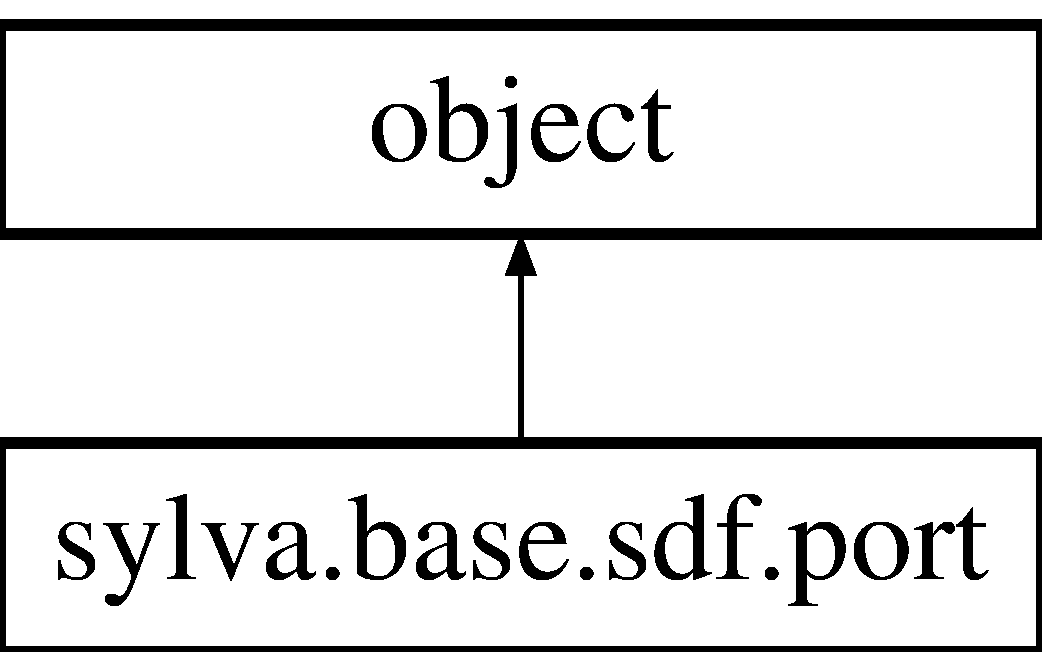
\includegraphics[height=2.000000cm]{classsylva_1_1base_1_1sdf_1_1port}
\end{center}
\end{figure}
\subsection*{Public Member Functions}
\begin{DoxyCompactItemize}
\item 
def \hyperlink{classsylva_1_1base_1_1sdf_1_1port_a648789838e7d9ff8d8cd26537ed006ad}{\+\_\+\+\_\+init\+\_\+\+\_\+} (self, \hyperlink{classsylva_1_1base_1_1sdf_1_1port_ace0eb23bb9f3e4a75e6a94f0961a6f99}{name}=\textquotesingle{}no\+\_\+port\+\_\+name\textquotesingle{}, \hyperlink{classsylva_1_1base_1_1sdf_1_1port_a4ed6db96ef0a6fb3d9b8f36c59bf7bdd}{index}=0, \hyperlink{classsylva_1_1base_1_1sdf_1_1port_af04b13138d55895bfd1083eb3e772f58}{type}=\hyperlink{classsylva_1_1base_1_1sdf_1_1_data_token_type}{Data\+Token\+Type}(\hyperlink{classsylva_1_1base_1_1sdf_1_1port_ace0eb23bb9f3e4a75e6a94f0961a6f99}{name}=\textquotesingle{}integer range 0 to 3\textquotesingle{}, size=2), \hyperlink{classsylva_1_1base_1_1sdf_1_1port_a628b66dd64830393bcf8d88b85023016}{count}=1)
\item 
def \hyperlink{classsylva_1_1base_1_1sdf_1_1port_a81a42bad6d299ec55b3d1482439d452f}{\+\_\+\+\_\+str\+\_\+\+\_\+} (self)
\item 
def \hyperlink{classsylva_1_1base_1_1sdf_1_1port_ae5c6adc9c86e717d12901d73699bb432}{clone} (self)
\item 
def \hyperlink{classsylva_1_1base_1_1sdf_1_1port_a19793d8e6190538a7d5cd014b08441b4}{serialize} (self)
\end{DoxyCompactItemize}
\subsection*{Public Attributes}
\begin{DoxyCompactItemize}
\item 
\hyperlink{classsylva_1_1base_1_1sdf_1_1port_ace0eb23bb9f3e4a75e6a94f0961a6f99}{name}
\item 
\hyperlink{classsylva_1_1base_1_1sdf_1_1port_a4ed6db96ef0a6fb3d9b8f36c59bf7bdd}{index}
\item 
\hyperlink{classsylva_1_1base_1_1sdf_1_1port_af04b13138d55895bfd1083eb3e772f58}{type}
\item 
\hyperlink{classsylva_1_1base_1_1sdf_1_1port_a628b66dd64830393bcf8d88b85023016}{count}
\end{DoxyCompactItemize}
\subsection*{Private Attributes}
\begin{DoxyCompactItemize}
\item 
\hyperlink{classsylva_1_1base_1_1sdf_1_1port_a14e2fb1373bce5c98b5f779012db8a0b}{\+\_\+\+\_\+repr\+\_\+\+\_\+}
\end{DoxyCompactItemize}


\subsection{Detailed Description}
\begin{DoxyVerb}  IO port class for an actor
  --------------------------

  The port is either input or output.
  The IO direction (input or output) is not defined in this class.
  A port emits or receives one data token per clock cycle.

  1. name: string, port name
  2. index: integer, port index in either input port list or output port list
  3. type: DataTokenType, data token type of this port.
    The width of the port is defined by `type`.
  4. count: integer, number of data tokens to be transferred via this port
\end{DoxyVerb}
 

Definition at line 57 of file sdf.\+py.



\subsection{Constructor \& Destructor Documentation}
\mbox{\Hypertarget{classsylva_1_1base_1_1sdf_1_1port_a648789838e7d9ff8d8cd26537ed006ad}\label{classsylva_1_1base_1_1sdf_1_1port_a648789838e7d9ff8d8cd26537ed006ad}} 
\index{sylva\+::base\+::sdf\+::port@{sylva\+::base\+::sdf\+::port}!\+\_\+\+\_\+init\+\_\+\+\_\+@{\+\_\+\+\_\+init\+\_\+\+\_\+}}
\index{\+\_\+\+\_\+init\+\_\+\+\_\+@{\+\_\+\+\_\+init\+\_\+\+\_\+}!sylva\+::base\+::sdf\+::port@{sylva\+::base\+::sdf\+::port}}
\subsubsection{\texorpdfstring{\+\_\+\+\_\+init\+\_\+\+\_\+()}{\_\_init\_\_()}}
{\footnotesize\ttfamily def sylva.\+base.\+sdf.\+port.\+\_\+\+\_\+init\+\_\+\+\_\+ (\begin{DoxyParamCaption}\item[{}]{self,  }\item[{}]{name = {\ttfamily \textquotesingle{}no\+\_\+port\+\_\+name\textquotesingle{}},  }\item[{}]{index = {\ttfamily 0},  }\item[{}]{type = {\ttfamily \hyperlink{classsylva_1_1base_1_1sdf_1_1_data_token_type}{Data\+Token\+Type}(\hyperlink{classsylva_1_1base_1_1sdf_1_1port_ace0eb23bb9f3e4a75e6a94f0961a6f99}{name}=\textquotesingle{}integer~range~0~to~3\textquotesingle{},~size=2)},  }\item[{}]{count = {\ttfamily 1} }\end{DoxyParamCaption})}



Definition at line 76 of file sdf.\+py.


\begin{DoxyCode}
76                      count=1):
77 
78             self.name = name
79             self.index = index
80             self.type = type
81             self.count = count
82 
83             self.\_\_repr\_\_ = self.\_\_str\_\_
84 
\end{DoxyCode}


\subsection{Member Function Documentation}
\mbox{\Hypertarget{classsylva_1_1base_1_1sdf_1_1port_a81a42bad6d299ec55b3d1482439d452f}\label{classsylva_1_1base_1_1sdf_1_1port_a81a42bad6d299ec55b3d1482439d452f}} 
\index{sylva\+::base\+::sdf\+::port@{sylva\+::base\+::sdf\+::port}!\+\_\+\+\_\+str\+\_\+\+\_\+@{\+\_\+\+\_\+str\+\_\+\+\_\+}}
\index{\+\_\+\+\_\+str\+\_\+\+\_\+@{\+\_\+\+\_\+str\+\_\+\+\_\+}!sylva\+::base\+::sdf\+::port@{sylva\+::base\+::sdf\+::port}}
\subsubsection{\texorpdfstring{\+\_\+\+\_\+str\+\_\+\+\_\+()}{\_\_str\_\_()}}
{\footnotesize\ttfamily def sylva.\+base.\+sdf.\+port.\+\_\+\+\_\+str\+\_\+\+\_\+ (\begin{DoxyParamCaption}\item[{}]{self }\end{DoxyParamCaption})}



Definition at line 85 of file sdf.\+py.



References sylva.\+base.\+sdf.\+port.\+count, sylva.\+base.\+fimp.\+fimp.\+index, sylva.\+base.\+sdf.\+port.\+index, sylva.\+base.\+sdf.\+Data\+Token\+Type.\+name, sylva.\+base.\+fimp.\+fimp.\+name, sylva.\+base.\+sdf.\+port.\+name, sylva.\+base.\+fimp.\+fimp\+\_\+set.\+name, sylva.\+base.\+fimp.\+fimp\+\_\+lib.\+name, sylva.\+base.\+fimp.\+fimp.\+type, and sylva.\+base.\+sdf.\+port.\+type.



Referenced by sylva.\+code\+\_\+generation.\+air.\+Bass\+Object.\+\_\+\+\_\+repr\+\_\+\+\_\+().


\begin{DoxyCode}
85         \textcolor{keyword}{def }\_\_str\_\_(self):
86             \textcolor{keywordflow}{return} \textcolor{stringliteral}{'SDF port %s index %s type %s count %s'} \(\backslash\)
87                 % (self.name, self.index, self.type, self.count)
88 
\end{DoxyCode}
\mbox{\Hypertarget{classsylva_1_1base_1_1sdf_1_1port_ae5c6adc9c86e717d12901d73699bb432}\label{classsylva_1_1base_1_1sdf_1_1port_ae5c6adc9c86e717d12901d73699bb432}} 
\index{sylva\+::base\+::sdf\+::port@{sylva\+::base\+::sdf\+::port}!clone@{clone}}
\index{clone@{clone}!sylva\+::base\+::sdf\+::port@{sylva\+::base\+::sdf\+::port}}
\subsubsection{\texorpdfstring{clone()}{clone()}}
{\footnotesize\ttfamily def sylva.\+base.\+sdf.\+port.\+clone (\begin{DoxyParamCaption}\item[{}]{self }\end{DoxyParamCaption})}



Definition at line 89 of file sdf.\+py.



References sylva.\+base.\+sdf.\+port.\+count, sylva.\+base.\+fimp.\+fimp.\+index, sylva.\+base.\+sdf.\+port.\+index, sylva.\+base.\+sdf.\+Data\+Token\+Type.\+name, sylva.\+base.\+fimp.\+fimp.\+name, sylva.\+base.\+sdf.\+port.\+name, sylva.\+base.\+fimp.\+fimp\+\_\+set.\+name, sylva.\+base.\+fimp.\+fimp\+\_\+lib.\+name, sylva.\+base.\+fimp.\+fimp.\+type, and sylva.\+base.\+sdf.\+port.\+type.


\begin{DoxyCode}
89         \textcolor{keyword}{def }clone(self):
90             \textcolor{keywordflow}{return} port(self.name, self.index, self.type, self.count)
91 
\end{DoxyCode}
\mbox{\Hypertarget{classsylva_1_1base_1_1sdf_1_1port_a19793d8e6190538a7d5cd014b08441b4}\label{classsylva_1_1base_1_1sdf_1_1port_a19793d8e6190538a7d5cd014b08441b4}} 
\index{sylva\+::base\+::sdf\+::port@{sylva\+::base\+::sdf\+::port}!serialize@{serialize}}
\index{serialize@{serialize}!sylva\+::base\+::sdf\+::port@{sylva\+::base\+::sdf\+::port}}
\subsubsection{\texorpdfstring{serialize()}{serialize()}}
{\footnotesize\ttfamily def sylva.\+base.\+sdf.\+port.\+serialize (\begin{DoxyParamCaption}\item[{}]{self }\end{DoxyParamCaption})}



Definition at line 92 of file sdf.\+py.



References sylva.\+base.\+sdf.\+port.\+count, sylva.\+base.\+fimp.\+fimp.\+index, sylva.\+base.\+sdf.\+port.\+index, sylva.\+base.\+sdf.\+Data\+Token\+Type.\+name, sylva.\+base.\+fimp.\+fimp.\+name, sylva.\+base.\+sdf.\+port.\+name, sylva.\+base.\+fimp.\+fimp\+\_\+set.\+name, sylva.\+base.\+fimp.\+fimp\+\_\+lib.\+name, sylva.\+base.\+fimp.\+fimp.\+type, and sylva.\+base.\+sdf.\+port.\+type.


\begin{DoxyCode}
92         \textcolor{keyword}{def }serialize(self):
93             \textcolor{keywordflow}{return} \{\textcolor{stringliteral}{'name'}: self.name,
94                     \textcolor{stringliteral}{'index'}: self.index,
95                     \textcolor{stringliteral}{'type'}: self.type.serialize(),
96                     \textcolor{stringliteral}{'count'}: self.count\}
97 
98     \textcolor{keyword}{def }\hyperlink{namespacesylva_1_1base_1_1sdf_a72bbd0e1cd0a666269ac3f17427954b8}{load\_sdf\_port}(json\_dict):
\end{DoxyCode}


\subsection{Member Data Documentation}
\mbox{\Hypertarget{classsylva_1_1base_1_1sdf_1_1port_a14e2fb1373bce5c98b5f779012db8a0b}\label{classsylva_1_1base_1_1sdf_1_1port_a14e2fb1373bce5c98b5f779012db8a0b}} 
\index{sylva\+::base\+::sdf\+::port@{sylva\+::base\+::sdf\+::port}!\+\_\+\+\_\+repr\+\_\+\+\_\+@{\+\_\+\+\_\+repr\+\_\+\+\_\+}}
\index{\+\_\+\+\_\+repr\+\_\+\+\_\+@{\+\_\+\+\_\+repr\+\_\+\+\_\+}!sylva\+::base\+::sdf\+::port@{sylva\+::base\+::sdf\+::port}}
\subsubsection{\texorpdfstring{\+\_\+\+\_\+repr\+\_\+\+\_\+}{\_\_repr\_\_}}
{\footnotesize\ttfamily sylva.\+base.\+sdf.\+port.\+\_\+\+\_\+repr\+\_\+\+\_\+\hspace{0.3cm}{\ttfamily [private]}}



Definition at line 83 of file sdf.\+py.

\mbox{\Hypertarget{classsylva_1_1base_1_1sdf_1_1port_a628b66dd64830393bcf8d88b85023016}\label{classsylva_1_1base_1_1sdf_1_1port_a628b66dd64830393bcf8d88b85023016}} 
\index{sylva\+::base\+::sdf\+::port@{sylva\+::base\+::sdf\+::port}!count@{count}}
\index{count@{count}!sylva\+::base\+::sdf\+::port@{sylva\+::base\+::sdf\+::port}}
\subsubsection{\texorpdfstring{count}{count}}
{\footnotesize\ttfamily sylva.\+base.\+sdf.\+port.\+count}



Definition at line 81 of file sdf.\+py.



Referenced by sylva.\+base.\+sdf.\+port.\+\_\+\+\_\+str\+\_\+\+\_\+(), sylva.\+base.\+sdf.\+port.\+clone(), and sylva.\+base.\+sdf.\+port.\+serialize().

\mbox{\Hypertarget{classsylva_1_1base_1_1sdf_1_1port_a4ed6db96ef0a6fb3d9b8f36c59bf7bdd}\label{classsylva_1_1base_1_1sdf_1_1port_a4ed6db96ef0a6fb3d9b8f36c59bf7bdd}} 
\index{sylva\+::base\+::sdf\+::port@{sylva\+::base\+::sdf\+::port}!index@{index}}
\index{index@{index}!sylva\+::base\+::sdf\+::port@{sylva\+::base\+::sdf\+::port}}
\subsubsection{\texorpdfstring{index}{index}}
{\footnotesize\ttfamily sylva.\+base.\+sdf.\+port.\+index}



Definition at line 79 of file sdf.\+py.



Referenced by sylva.\+base.\+sdf.\+port.\+\_\+\+\_\+str\+\_\+\+\_\+(), sylva.\+glic.\+glic.\+state.\+\_\+\+\_\+str\+\_\+\+\_\+(), sylva.\+base.\+sdf.\+actor.\+\_\+\+\_\+str\+\_\+\+\_\+(), sylva.\+base.\+sdf.\+port.\+clone(), sylva.\+base.\+sdf.\+actor.\+clone(), sylva.\+base.\+sdf.\+port.\+serialize(), sylva.\+glic.\+glic.\+state.\+serialize(), and sylva.\+base.\+sdf.\+actor.\+serialize().

\mbox{\Hypertarget{classsylva_1_1base_1_1sdf_1_1port_ace0eb23bb9f3e4a75e6a94f0961a6f99}\label{classsylva_1_1base_1_1sdf_1_1port_ace0eb23bb9f3e4a75e6a94f0961a6f99}} 
\index{sylva\+::base\+::sdf\+::port@{sylva\+::base\+::sdf\+::port}!name@{name}}
\index{name@{name}!sylva\+::base\+::sdf\+::port@{sylva\+::base\+::sdf\+::port}}
\subsubsection{\texorpdfstring{name}{name}}
{\footnotesize\ttfamily sylva.\+base.\+sdf.\+port.\+name}



Definition at line 78 of file sdf.\+py.



Referenced by sylva.\+frontend.\+mdl\+\_\+reader.\+simulink\+\_\+model.\+\_\+\+\_\+str\+\_\+\+\_\+(), sylva.\+frontend.\+mdl\+\_\+reader.\+simulink\+\_\+system.\+\_\+\+\_\+str\+\_\+\+\_\+(), sylva.\+base.\+sdf.\+port.\+\_\+\+\_\+str\+\_\+\+\_\+(), sylva.\+glic.\+glic.\+control.\+\_\+\+\_\+str\+\_\+\+\_\+(), sylva.\+base.\+sdf.\+actor.\+\_\+\+\_\+str\+\_\+\+\_\+(), sylva.\+base.\+sdf.\+port.\+clone(), sylva.\+base.\+sdf.\+actor.\+clone(), sylva.\+base.\+sdf.\+port.\+serialize(), sylva.\+dse.\+dse.\+system\+\_\+model.\+serialize(), sylva.\+glic.\+glic.\+control.\+serialize(), and sylva.\+base.\+sdf.\+actor.\+serialize().

\mbox{\Hypertarget{classsylva_1_1base_1_1sdf_1_1port_af04b13138d55895bfd1083eb3e772f58}\label{classsylva_1_1base_1_1sdf_1_1port_af04b13138d55895bfd1083eb3e772f58}} 
\index{sylva\+::base\+::sdf\+::port@{sylva\+::base\+::sdf\+::port}!type@{type}}
\index{type@{type}!sylva\+::base\+::sdf\+::port@{sylva\+::base\+::sdf\+::port}}
\subsubsection{\texorpdfstring{type}{type}}
{\footnotesize\ttfamily sylva.\+base.\+sdf.\+port.\+type}



Definition at line 80 of file sdf.\+py.



Referenced by sylva.\+base.\+sdf.\+port.\+\_\+\+\_\+str\+\_\+\+\_\+(), sylva.\+base.\+sdf.\+port.\+clone(), and sylva.\+base.\+sdf.\+port.\+serialize().



The documentation for this class was generated from the following file\+:\begin{DoxyCompactItemize}
\item 
base/\hyperlink{sdf_8py}{sdf.\+py}\end{DoxyCompactItemize}

\hypertarget{classsylva_1_1code__generation_1_1air_1_1_port_and_actions}{}\section{sylva.\+code\+\_\+generation.\+air.\+Port\+And\+Actions Class Reference}
\label{classsylva_1_1code__generation_1_1air_1_1_port_and_actions}\index{sylva.\+code\+\_\+generation.\+air.\+Port\+And\+Actions@{sylva.\+code\+\_\+generation.\+air.\+Port\+And\+Actions}}
Inheritance diagram for sylva.\+code\+\_\+generation.\+air.\+Port\+And\+Actions\+:\begin{figure}[H]
\begin{center}
\leavevmode
\includegraphics[height=2.000000cm]{classsylva_1_1code__generation_1_1air_1_1_port_and_actions}
\end{center}
\end{figure}
\subsection*{Public Member Functions}
\begin{DoxyCompactItemize}
\item 
def \hyperlink{classsylva_1_1code__generation_1_1air_1_1_port_and_actions_a099f5352bd153f64b013fe50a8358308}{\+\_\+\+\_\+init\+\_\+\+\_\+} (self, \hyperlink{classsylva_1_1code__generation_1_1air_1_1_port_and_actions_a6b5a21780c1b3cc8879c05a5dfdd65bf}{port}, \hyperlink{classsylva_1_1code__generation_1_1air_1_1_port_and_actions_aaeb765c205fcb8c38025428542025ba7}{actions})
\item 
def \hyperlink{classsylva_1_1code__generation_1_1air_1_1_bass_object_a2c164720220479369c29db97b67aabe8}{\+\_\+\+\_\+str\+\_\+\+\_\+} (self)
\item 
def \hyperlink{classsylva_1_1code__generation_1_1air_1_1_bass_object_a17548b84b2a55240a429506aed418292}{\+\_\+\+\_\+repr\+\_\+\+\_\+} (self)
\end{DoxyCompactItemize}
\subsection*{Public Attributes}
\begin{DoxyCompactItemize}
\item 
\hyperlink{classsylva_1_1code__generation_1_1air_1_1_port_and_actions_a6b5a21780c1b3cc8879c05a5dfdd65bf}{port}
\item 
\hyperlink{classsylva_1_1code__generation_1_1air_1_1_port_and_actions_aaeb765c205fcb8c38025428542025ba7}{actions}
\end{DoxyCompactItemize}


\subsection{Detailed Description}


Definition at line 105 of file air.\+py.



\subsection{Constructor \& Destructor Documentation}
\mbox{\Hypertarget{classsylva_1_1code__generation_1_1air_1_1_port_and_actions_a099f5352bd153f64b013fe50a8358308}\label{classsylva_1_1code__generation_1_1air_1_1_port_and_actions_a099f5352bd153f64b013fe50a8358308}} 
\index{sylva\+::code\+\_\+generation\+::air\+::\+Port\+And\+Actions@{sylva\+::code\+\_\+generation\+::air\+::\+Port\+And\+Actions}!\+\_\+\+\_\+init\+\_\+\+\_\+@{\+\_\+\+\_\+init\+\_\+\+\_\+}}
\index{\+\_\+\+\_\+init\+\_\+\+\_\+@{\+\_\+\+\_\+init\+\_\+\+\_\+}!sylva\+::code\+\_\+generation\+::air\+::\+Port\+And\+Actions@{sylva\+::code\+\_\+generation\+::air\+::\+Port\+And\+Actions}}
\subsubsection{\texorpdfstring{\+\_\+\+\_\+init\+\_\+\+\_\+()}{\_\_init\_\_()}}
{\footnotesize\ttfamily def sylva.\+code\+\_\+generation.\+air.\+Port\+And\+Actions.\+\_\+\+\_\+init\+\_\+\+\_\+ (\begin{DoxyParamCaption}\item[{}]{self,  }\item[{}]{port,  }\item[{}]{actions }\end{DoxyParamCaption})}



Definition at line 106 of file air.\+py.


\begin{DoxyCode}
106   \textcolor{keyword}{def }\_\_init\_\_(self, port, actions) :
107     self.port = port
108     self.actions = actions
109 
\end{DoxyCode}


\subsection{Member Function Documentation}
\mbox{\Hypertarget{classsylva_1_1code__generation_1_1air_1_1_bass_object_a17548b84b2a55240a429506aed418292}\label{classsylva_1_1code__generation_1_1air_1_1_bass_object_a17548b84b2a55240a429506aed418292}} 
\index{sylva\+::code\+\_\+generation\+::air\+::\+Port\+And\+Actions@{sylva\+::code\+\_\+generation\+::air\+::\+Port\+And\+Actions}!\+\_\+\+\_\+repr\+\_\+\+\_\+@{\+\_\+\+\_\+repr\+\_\+\+\_\+}}
\index{\+\_\+\+\_\+repr\+\_\+\+\_\+@{\+\_\+\+\_\+repr\+\_\+\+\_\+}!sylva\+::code\+\_\+generation\+::air\+::\+Port\+And\+Actions@{sylva\+::code\+\_\+generation\+::air\+::\+Port\+And\+Actions}}
\subsubsection{\texorpdfstring{\+\_\+\+\_\+repr\+\_\+\+\_\+()}{\_\_repr\_\_()}}
{\footnotesize\ttfamily def sylva.\+code\+\_\+generation.\+air.\+Bass\+Object.\+\_\+\+\_\+repr\+\_\+\+\_\+ (\begin{DoxyParamCaption}\item[{}]{self }\end{DoxyParamCaption})\hspace{0.3cm}{\ttfamily [inherited]}}



Definition at line 91 of file air.\+py.



References sylva.\+base.\+sdf.\+Data\+Token\+Type.\+\_\+\+\_\+str\+\_\+\+\_\+(), sylva.\+base.\+sdf\+\_\+schedule.\+schedule.\+\_\+\+\_\+str\+\_\+\+\_\+(), sylva.\+base.\+sdf.\+port.\+\_\+\+\_\+str\+\_\+\+\_\+(), sylva.\+code\+\_\+generation.\+air.\+Bass\+Object.\+\_\+\+\_\+str\+\_\+\+\_\+(), sylva.\+base.\+fimp.\+fimp.\+\_\+\+\_\+str\+\_\+\+\_\+(), sylva.\+base.\+sdf.\+edge.\+\_\+\+\_\+str\+\_\+\+\_\+(), and sylva.\+base.\+sdf.\+actor.\+\_\+\+\_\+str\+\_\+\+\_\+().


\begin{DoxyCode}
91   \textcolor{keyword}{def }\hyperlink{namespacesylva_1_1code__generation_1_1floorplanner_a84f24b1e40f5425e9bb40ab45ccbd10f}{\_\_repr\_\_}(self) :
92     \textcolor{keywordflow}{return} self.\_\_str\_\_()
93 
\end{DoxyCode}
\mbox{\Hypertarget{classsylva_1_1code__generation_1_1air_1_1_bass_object_a2c164720220479369c29db97b67aabe8}\label{classsylva_1_1code__generation_1_1air_1_1_bass_object_a2c164720220479369c29db97b67aabe8}} 
\index{sylva\+::code\+\_\+generation\+::air\+::\+Port\+And\+Actions@{sylva\+::code\+\_\+generation\+::air\+::\+Port\+And\+Actions}!\+\_\+\+\_\+str\+\_\+\+\_\+@{\+\_\+\+\_\+str\+\_\+\+\_\+}}
\index{\+\_\+\+\_\+str\+\_\+\+\_\+@{\+\_\+\+\_\+str\+\_\+\+\_\+}!sylva\+::code\+\_\+generation\+::air\+::\+Port\+And\+Actions@{sylva\+::code\+\_\+generation\+::air\+::\+Port\+And\+Actions}}
\subsubsection{\texorpdfstring{\+\_\+\+\_\+str\+\_\+\+\_\+()}{\_\_str\_\_()}}
{\footnotesize\ttfamily def sylva.\+code\+\_\+generation.\+air.\+Bass\+Object.\+\_\+\+\_\+str\+\_\+\+\_\+ (\begin{DoxyParamCaption}\item[{}]{self }\end{DoxyParamCaption})\hspace{0.3cm}{\ttfamily [inherited]}}



Definition at line 89 of file air.\+py.



Referenced by sylva.\+code\+\_\+generation.\+air.\+Bass\+Object.\+\_\+\+\_\+repr\+\_\+\+\_\+().


\begin{DoxyCode}
89   \textcolor{keyword}{def }\_\_str\_\_(self) :
90     \textcolor{keywordflow}{return} str(self.\_\_dict\_\_)
\end{DoxyCode}


\subsection{Member Data Documentation}
\mbox{\Hypertarget{classsylva_1_1code__generation_1_1air_1_1_port_and_actions_aaeb765c205fcb8c38025428542025ba7}\label{classsylva_1_1code__generation_1_1air_1_1_port_and_actions_aaeb765c205fcb8c38025428542025ba7}} 
\index{sylva\+::code\+\_\+generation\+::air\+::\+Port\+And\+Actions@{sylva\+::code\+\_\+generation\+::air\+::\+Port\+And\+Actions}!actions@{actions}}
\index{actions@{actions}!sylva\+::code\+\_\+generation\+::air\+::\+Port\+And\+Actions@{sylva\+::code\+\_\+generation\+::air\+::\+Port\+And\+Actions}}
\subsubsection{\texorpdfstring{actions}{actions}}
{\footnotesize\ttfamily sylva.\+code\+\_\+generation.\+air.\+Port\+And\+Actions.\+actions}



Definition at line 108 of file air.\+py.

\mbox{\Hypertarget{classsylva_1_1code__generation_1_1air_1_1_port_and_actions_a6b5a21780c1b3cc8879c05a5dfdd65bf}\label{classsylva_1_1code__generation_1_1air_1_1_port_and_actions_a6b5a21780c1b3cc8879c05a5dfdd65bf}} 
\index{sylva\+::code\+\_\+generation\+::air\+::\+Port\+And\+Actions@{sylva\+::code\+\_\+generation\+::air\+::\+Port\+And\+Actions}!port@{port}}
\index{port@{port}!sylva\+::code\+\_\+generation\+::air\+::\+Port\+And\+Actions@{sylva\+::code\+\_\+generation\+::air\+::\+Port\+And\+Actions}}
\subsubsection{\texorpdfstring{port}{port}}
{\footnotesize\ttfamily sylva.\+code\+\_\+generation.\+air.\+Port\+And\+Actions.\+port}



Definition at line 107 of file air.\+py.



The documentation for this class was generated from the following file\+:\begin{DoxyCompactItemize}
\item 
code\+\_\+generation/\hyperlink{air_8py}{air.\+py}\end{DoxyCompactItemize}

\hypertarget{classsylva_1_1code__generation_1_1air_1_1_port_map_condition}{}\section{sylva.\+code\+\_\+generation.\+air.\+Port\+Map\+Condition Class Reference}
\label{classsylva_1_1code__generation_1_1air_1_1_port_map_condition}\index{sylva.\+code\+\_\+generation.\+air.\+Port\+Map\+Condition@{sylva.\+code\+\_\+generation.\+air.\+Port\+Map\+Condition}}


Inheritance diagram for sylva.\+code\+\_\+generation.\+air.\+Port\+Map\+Condition\+:\nopagebreak
\begin{figure}[H]
\begin{center}
\leavevmode
\includegraphics[width=209pt]{classsylva_1_1code__generation_1_1air_1_1_port_map_condition__inherit__graph}
\end{center}
\end{figure}
\subsection*{Public Member Functions}
\begin{DoxyCompactItemize}
\item 
def \hyperlink{classsylva_1_1code__generation_1_1air_1_1_port_map_condition_ae9d4fe40feaa0466075ab2ea74bdb7ce}{\+\_\+\+\_\+init\+\_\+\+\_\+} (self, \hyperlink{classsylva_1_1code__generation_1_1air_1_1_port_map_condition_a8144ca86c7e62e6bc09ab9b21322e146}{control\+\_\+port}, \hyperlink{classsylva_1_1code__generation_1_1air_1_1_port_map_condition_a98936107f0135352da9608e71fcdf69e}{valid\+\_\+values}, \hyperlink{classsylva_1_1code__generation_1_1air_1_1_port_map_condition_a88a75f6cca1f9c1db5bd699c6e82f191}{input\+\_\+port})
\end{DoxyCompactItemize}
\subsection*{Public Attributes}
\begin{DoxyCompactItemize}
\item 
\hyperlink{classsylva_1_1code__generation_1_1air_1_1_port_map_condition_a8144ca86c7e62e6bc09ab9b21322e146}{control\+\_\+port}
\item 
\hyperlink{classsylva_1_1code__generation_1_1air_1_1_port_map_condition_a98936107f0135352da9608e71fcdf69e}{valid\+\_\+values}
\item 
\hyperlink{classsylva_1_1code__generation_1_1air_1_1_port_map_condition_a88a75f6cca1f9c1db5bd699c6e82f191}{input\+\_\+port}
\end{DoxyCompactItemize}


\subsection{Detailed Description}


Definition at line 111 of file air.\+py.



\subsection{Constructor \& Destructor Documentation}
\mbox{\Hypertarget{classsylva_1_1code__generation_1_1air_1_1_port_map_condition_ae9d4fe40feaa0466075ab2ea74bdb7ce}\label{classsylva_1_1code__generation_1_1air_1_1_port_map_condition_ae9d4fe40feaa0466075ab2ea74bdb7ce}} 
\index{sylva\+::code\+\_\+generation\+::air\+::\+Port\+Map\+Condition@{sylva\+::code\+\_\+generation\+::air\+::\+Port\+Map\+Condition}!\+\_\+\+\_\+init\+\_\+\+\_\+@{\+\_\+\+\_\+init\+\_\+\+\_\+}}
\index{\+\_\+\+\_\+init\+\_\+\+\_\+@{\+\_\+\+\_\+init\+\_\+\+\_\+}!sylva\+::code\+\_\+generation\+::air\+::\+Port\+Map\+Condition@{sylva\+::code\+\_\+generation\+::air\+::\+Port\+Map\+Condition}}
\subsubsection{\texorpdfstring{\+\_\+\+\_\+init\+\_\+\+\_\+()}{\_\_init\_\_()}}
{\footnotesize\ttfamily def sylva.\+code\+\_\+generation.\+air.\+Port\+Map\+Condition.\+\_\+\+\_\+init\+\_\+\+\_\+ (\begin{DoxyParamCaption}\item[{}]{self,  }\item[{}]{control\+\_\+port,  }\item[{}]{valid\+\_\+values,  }\item[{}]{input\+\_\+port }\end{DoxyParamCaption})}



Definition at line 113 of file air.\+py.


\begin{DoxyCode}
113     \textcolor{keyword}{def }\_\_init\_\_(self, control\_port, valid\_values, input\_port):
114         self.control\_port = control\_port
115         self.valid\_values = valid\_values
116         self.input\_port = input\_port
117 
118 
\end{DoxyCode}


\subsection{Member Data Documentation}
\mbox{\Hypertarget{classsylva_1_1code__generation_1_1air_1_1_port_map_condition_a8144ca86c7e62e6bc09ab9b21322e146}\label{classsylva_1_1code__generation_1_1air_1_1_port_map_condition_a8144ca86c7e62e6bc09ab9b21322e146}} 
\index{sylva\+::code\+\_\+generation\+::air\+::\+Port\+Map\+Condition@{sylva\+::code\+\_\+generation\+::air\+::\+Port\+Map\+Condition}!control\+\_\+port@{control\+\_\+port}}
\index{control\+\_\+port@{control\+\_\+port}!sylva\+::code\+\_\+generation\+::air\+::\+Port\+Map\+Condition@{sylva\+::code\+\_\+generation\+::air\+::\+Port\+Map\+Condition}}
\subsubsection{\texorpdfstring{control\+\_\+port}{control\_port}}
{\footnotesize\ttfamily sylva.\+code\+\_\+generation.\+air.\+Port\+Map\+Condition.\+control\+\_\+port}



Definition at line 114 of file air.\+py.

\mbox{\Hypertarget{classsylva_1_1code__generation_1_1air_1_1_port_map_condition_a88a75f6cca1f9c1db5bd699c6e82f191}\label{classsylva_1_1code__generation_1_1air_1_1_port_map_condition_a88a75f6cca1f9c1db5bd699c6e82f191}} 
\index{sylva\+::code\+\_\+generation\+::air\+::\+Port\+Map\+Condition@{sylva\+::code\+\_\+generation\+::air\+::\+Port\+Map\+Condition}!input\+\_\+port@{input\+\_\+port}}
\index{input\+\_\+port@{input\+\_\+port}!sylva\+::code\+\_\+generation\+::air\+::\+Port\+Map\+Condition@{sylva\+::code\+\_\+generation\+::air\+::\+Port\+Map\+Condition}}
\subsubsection{\texorpdfstring{input\+\_\+port}{input\_port}}
{\footnotesize\ttfamily sylva.\+code\+\_\+generation.\+air.\+Port\+Map\+Condition.\+input\+\_\+port}



Definition at line 116 of file air.\+py.

\mbox{\Hypertarget{classsylva_1_1code__generation_1_1air_1_1_port_map_condition_a98936107f0135352da9608e71fcdf69e}\label{classsylva_1_1code__generation_1_1air_1_1_port_map_condition_a98936107f0135352da9608e71fcdf69e}} 
\index{sylva\+::code\+\_\+generation\+::air\+::\+Port\+Map\+Condition@{sylva\+::code\+\_\+generation\+::air\+::\+Port\+Map\+Condition}!valid\+\_\+values@{valid\+\_\+values}}
\index{valid\+\_\+values@{valid\+\_\+values}!sylva\+::code\+\_\+generation\+::air\+::\+Port\+Map\+Condition@{sylva\+::code\+\_\+generation\+::air\+::\+Port\+Map\+Condition}}
\subsubsection{\texorpdfstring{valid\+\_\+values}{valid\_values}}
{\footnotesize\ttfamily sylva.\+code\+\_\+generation.\+air.\+Port\+Map\+Condition.\+valid\+\_\+values}



Definition at line 115 of file air.\+py.



The documentation for this class was generated from the following file\+:\begin{DoxyCompactItemize}
\item 
code\+\_\+generation/\hyperlink{air_8py}{air.\+py}\end{DoxyCompactItemize}

\hypertarget{classsylva_1_1misc_1_1plot_1_1rectangle}{}\section{sylva.\+misc.\+plot.\+rectangle Class Reference}
\label{classsylva_1_1misc_1_1plot_1_1rectangle}\index{sylva.\+misc.\+plot.\+rectangle@{sylva.\+misc.\+plot.\+rectangle}}


Inheritance diagram for sylva.\+misc.\+plot.\+rectangle\+:\nopagebreak
\begin{figure}[H]
\begin{center}
\leavevmode
\includegraphics[width=204pt]{classsylva_1_1misc_1_1plot_1_1rectangle__inherit__graph}
\end{center}
\end{figure}
\subsection*{Public Member Functions}
\begin{DoxyCompactItemize}
\item 
def \hyperlink{classsylva_1_1misc_1_1plot_1_1rectangle_aa01b01f82b1ab5f4e7fb2bba478a13e6}{\+\_\+\+\_\+init\+\_\+\+\_\+} (self, \hyperlink{classsylva_1_1misc_1_1plot_1_1rectangle_ad81773b097d59cb5c67b7e06ab6c022c}{width}, \hyperlink{classsylva_1_1misc_1_1plot_1_1rectangle_aa6bbc8337c03f65fc0097a8013f9c475}{height}, \hyperlink{classsylva_1_1misc_1_1plot_1_1rectangle_aea9a12e78d03675a8af2682b9bbd656b}{name}=None, \hyperlink{classsylva_1_1misc_1_1plot_1_1rectangle_a1bf48f6505e5a549e1056f6a8cb0b454}{xy}=None, \hyperlink{classsylva_1_1misc_1_1plot_1_1rectangle_a935b64e6f087b6ab153df8a45e6dd72d}{x}=None, \hyperlink{classsylva_1_1misc_1_1plot_1_1rectangle_a3067088c7894de27d5a3338077ef027b}{y}=None)
\item 
def \hyperlink{classsylva_1_1misc_1_1plot_1_1rectangle_a95db845fde73592eef007ab940b8b140}{overlaps} (self, other)
\item 
def \hyperlink{classsylva_1_1misc_1_1plot_1_1rectangle_a097b8412cf074afb98f7f88cd0e2f1bc}{\+\_\+\+\_\+contains\+\_\+\+\_\+} (self, other)
\item 
def \hyperlink{classsylva_1_1misc_1_1plot_1_1rectangle_a935b64e6f087b6ab153df8a45e6dd72d}{x} (self)
\item 
def \hyperlink{classsylva_1_1misc_1_1plot_1_1rectangle_a94fe87f391637f1ddf6ab629ffea76a1}{x} (self, value)
\item 
def \hyperlink{classsylva_1_1misc_1_1plot_1_1rectangle_a3067088c7894de27d5a3338077ef027b}{y} (self)
\item 
def \hyperlink{classsylva_1_1misc_1_1plot_1_1rectangle_a99edbd1ca0485e36233c604797adcda8}{y} (self, value)
\item 
def \hyperlink{classsylva_1_1misc_1_1plot_1_1rectangle_a50bdb9a7a95b6e03a66ce8031649ff9f}{right} (self)
\item 
def \hyperlink{classsylva_1_1misc_1_1plot_1_1rectangle_a4080bf5f63cc48132e480b458369af41}{left} (self)
\item 
def \hyperlink{classsylva_1_1misc_1_1plot_1_1rectangle_ac5b4d8952847953f5aa329fb839b63ad}{top} (self)
\item 
def \hyperlink{classsylva_1_1misc_1_1plot_1_1rectangle_a1ad220e20ea15beaeafdd814705d570e}{bottom} (self)
\item 
def \hyperlink{classsylva_1_1misc_1_1plot_1_1rectangle_a54324a7b1be1bd85655ee60686d5944f}{top\+\_\+right} (self)
\item 
def \hyperlink{classsylva_1_1misc_1_1plot_1_1rectangle_a657018c2fcbc892047da2f18166aae85}{bottom\+\_\+right} (self)
\item 
def \hyperlink{classsylva_1_1misc_1_1plot_1_1rectangle_ac763b52f6d533f4b006421eae5f81b56}{top\+\_\+left} (self)
\item 
def \hyperlink{classsylva_1_1misc_1_1plot_1_1rectangle_a7c8c635a0a782c8e304f7440b74d8066}{bottom\+\_\+left} (self)
\item 
def \hyperlink{classsylva_1_1misc_1_1plot_1_1rectangle_a0466258315b096cd7f4e1918a1007488}{center} (self)
\item 
def \hyperlink{classsylva_1_1misc_1_1plot_1_1rectangle_a6395db39d40526291589390d31437f80}{pixel\+\_\+map} (self)
\item 
def \hyperlink{classsylva_1_1misc_1_1plot_1_1rectangle_af3defb54fedda1e1f8d886e5f840bb72}{get\+\_\+patch} (self, style=None)
\item 
def \hyperlink{classsylva_1_1misc_1_1plot_1_1rectangle_a614690234b91159164255ffc1a32f8be}{place\+\_\+right\+\_\+of} (self, other)
\item 
def \hyperlink{classsylva_1_1misc_1_1plot_1_1rectangle_ad468b38c9b5c95f14e5a6dec5d064cb1}{place\+\_\+left\+\_\+of} (self, other)
\item 
def \hyperlink{classsylva_1_1misc_1_1plot_1_1rectangle_ab0cdba67562bf45f97399b1e4529d6ac}{place\+\_\+above\+\_\+of} (self, other)
\item 
def \hyperlink{classsylva_1_1misc_1_1plot_1_1rectangle_aab959379faa71fa2fff5f1797207078b}{place\+\_\+below\+\_\+of} (self, other)
\end{DoxyCompactItemize}
\subsection*{Public Attributes}
\begin{DoxyCompactItemize}
\item 
\hyperlink{classsylva_1_1misc_1_1plot_1_1rectangle_a1bf48f6505e5a549e1056f6a8cb0b454}{xy}
\item 
\hyperlink{classsylva_1_1misc_1_1plot_1_1rectangle_aea9a12e78d03675a8af2682b9bbd656b}{name}
\item 
\hyperlink{classsylva_1_1misc_1_1plot_1_1rectangle_ad81773b097d59cb5c67b7e06ab6c022c}{width}
\item 
\hyperlink{classsylva_1_1misc_1_1plot_1_1rectangle_aa6bbc8337c03f65fc0097a8013f9c475}{height}
\end{DoxyCompactItemize}


\subsection{Detailed Description}


Definition at line 228 of file plot.\+py.



\subsection{Constructor \& Destructor Documentation}
\mbox{\Hypertarget{classsylva_1_1misc_1_1plot_1_1rectangle_aa01b01f82b1ab5f4e7fb2bba478a13e6}\label{classsylva_1_1misc_1_1plot_1_1rectangle_aa01b01f82b1ab5f4e7fb2bba478a13e6}} 
\index{sylva\+::misc\+::plot\+::rectangle@{sylva\+::misc\+::plot\+::rectangle}!\+\_\+\+\_\+init\+\_\+\+\_\+@{\+\_\+\+\_\+init\+\_\+\+\_\+}}
\index{\+\_\+\+\_\+init\+\_\+\+\_\+@{\+\_\+\+\_\+init\+\_\+\+\_\+}!sylva\+::misc\+::plot\+::rectangle@{sylva\+::misc\+::plot\+::rectangle}}
\subsubsection{\texorpdfstring{\+\_\+\+\_\+init\+\_\+\+\_\+()}{\_\_init\_\_()}}
{\footnotesize\ttfamily def sylva.\+misc.\+plot.\+rectangle.\+\_\+\+\_\+init\+\_\+\+\_\+ (\begin{DoxyParamCaption}\item[{}]{self,  }\item[{}]{width,  }\item[{}]{height,  }\item[{}]{name = {\ttfamily None},  }\item[{}]{xy = {\ttfamily None},  }\item[{}]{x = {\ttfamily None},  }\item[{}]{y = {\ttfamily None} }\end{DoxyParamCaption})}



Definition at line 231 of file plot.\+py.


\begin{DoxyCode}
231                      xy=\textcolor{keywordtype}{None}, x=\textcolor{keywordtype}{None}, y=\textcolor{keywordtype}{None}):
232 
233             \textcolor{comment}{# top-left position}
234             self.xy = xy \textcolor{keywordflow}{or} point(x, y)
235             self.name = name \textcolor{keywordflow}{or} str(self.xy)
236             self.width = width
237             self.height = height
238 
\end{DoxyCode}


\subsection{Member Function Documentation}
\mbox{\Hypertarget{classsylva_1_1misc_1_1plot_1_1rectangle_a097b8412cf074afb98f7f88cd0e2f1bc}\label{classsylva_1_1misc_1_1plot_1_1rectangle_a097b8412cf074afb98f7f88cd0e2f1bc}} 
\index{sylva\+::misc\+::plot\+::rectangle@{sylva\+::misc\+::plot\+::rectangle}!\+\_\+\+\_\+contains\+\_\+\+\_\+@{\+\_\+\+\_\+contains\+\_\+\+\_\+}}
\index{\+\_\+\+\_\+contains\+\_\+\+\_\+@{\+\_\+\+\_\+contains\+\_\+\+\_\+}!sylva\+::misc\+::plot\+::rectangle@{sylva\+::misc\+::plot\+::rectangle}}
\subsubsection{\texorpdfstring{\+\_\+\+\_\+contains\+\_\+\+\_\+()}{\_\_contains\_\_()}}
{\footnotesize\ttfamily def sylva.\+misc.\+plot.\+rectangle.\+\_\+\+\_\+contains\+\_\+\+\_\+ (\begin{DoxyParamCaption}\item[{}]{self,  }\item[{}]{other }\end{DoxyParamCaption})}



Definition at line 247 of file plot.\+py.



References sylva.\+misc.\+plot.\+rectangle.\+bottom(), sylva.\+misc.\+plot.\+rectangle.\+bottom\+\_\+left(), sylva.\+misc.\+plot.\+rectangle.\+bottom\+\_\+right(), sylva.\+misc.\+plot.\+rectangle.\+left(), sylva.\+misc.\+plot.\+rectangle.\+right(), sylva.\+misc.\+plot.\+rectangle.\+top(), sylva.\+misc.\+plot.\+rectangle.\+top\+\_\+left(), and sylva.\+misc.\+plot.\+rectangle.\+top\+\_\+right().


\begin{DoxyCode}
247         \textcolor{keyword}{def }\_\_contains\_\_(self, other):
248             \textcolor{keywordflow}{if} isinstance(other, rectangle):
249                 \textcolor{keywordflow}{return} self.top\_left \textcolor{keywordflow}{in} other \(\backslash\)
250                     \textcolor{keywordflow}{or} self.top\_right \textcolor{keywordflow}{in} other \(\backslash\)
251                     \textcolor{keywordflow}{or} self.bottom\_left \textcolor{keywordflow}{in} other \(\backslash\)
252                     \textcolor{keywordflow}{or} self.bottom\_right \textcolor{keywordflow}{in} other
253             \textcolor{keywordflow}{elif} isinstance(other, point):
254                 x\_in\_range = self.left.x <= other.x <= self.right.x
255                 y\_in\_range = self.top.y <= other.y <= self.bottom.y
256                 \textcolor{keywordflow}{return} x\_in\_range \textcolor{keywordflow}{and} y\_in\_range
257             \textcolor{keywordflow}{return} \textcolor{keyword}{False}
258 
\end{DoxyCode}
\mbox{\Hypertarget{classsylva_1_1misc_1_1plot_1_1rectangle_a1ad220e20ea15beaeafdd814705d570e}\label{classsylva_1_1misc_1_1plot_1_1rectangle_a1ad220e20ea15beaeafdd814705d570e}} 
\index{sylva\+::misc\+::plot\+::rectangle@{sylva\+::misc\+::plot\+::rectangle}!bottom@{bottom}}
\index{bottom@{bottom}!sylva\+::misc\+::plot\+::rectangle@{sylva\+::misc\+::plot\+::rectangle}}
\subsubsection{\texorpdfstring{bottom()}{bottom()}}
{\footnotesize\ttfamily def sylva.\+misc.\+plot.\+rectangle.\+bottom (\begin{DoxyParamCaption}\item[{}]{self }\end{DoxyParamCaption})}



Definition at line 294 of file plot.\+py.



References sylva.\+base.\+cgra.\+C\+G\+R\+A.\+height, sylva.\+base.\+cgra(\+D\+E\+S\+K\+T\+O\+P-\/\+D3\+I\+R\+S\+O\+A 的冲突副本 2017-\/05-\/19).\+C\+G\+R\+A.\+height, sylva.\+base.\+cgra(\+D\+E\+S\+K\+T\+O\+P-\/\+D3\+I\+R\+S\+O\+A 的冲突副本 2017-\/05-\/22).\+C\+G\+R\+A.\+height, sylva.\+base.\+fimp(\+D\+E\+S\+K\+T\+O\+P-\/\+D3\+I\+R\+S\+O\+A 的冲突副本 2017-\/05-\/19).\+F\+I\+M\+P\+Cost.\+height, sylva.\+base.\+fimp.\+F\+I\+M\+P\+Cost.\+height, sylva.\+misc.\+plot.\+rectangle.\+height, sylva.\+base.\+cgra.\+C\+G\+R\+A.\+width, sylva.\+base.\+cgra(\+D\+E\+S\+K\+T\+O\+P-\/\+D3\+I\+R\+S\+O\+A 的冲突副本 2017-\/05-\/19).\+C\+G\+R\+A.\+width, sylva.\+base.\+cgra(\+D\+E\+S\+K\+T\+O\+P-\/\+D3\+I\+R\+S\+O\+A 的冲突副本 2017-\/05-\/22).\+C\+G\+R\+A.\+width, sylva.\+base.\+fimp(\+D\+E\+S\+K\+T\+O\+P-\/\+D3\+I\+R\+S\+O\+A 的冲突副本 2017-\/05-\/19).\+F\+I\+M\+P\+Cost.\+width, sylva.\+base.\+fimp.\+F\+I\+M\+P\+Cost.\+width, sylva.\+misc.\+plot.\+rectangle.\+width, sylva.\+code\+\_\+generation.\+floorplanner.\+floorplanner.\+x, sylva.\+misc.\+plot.\+point.\+x, sylva.\+misc.\+plot.\+rectangle.\+x(), sylva.\+base.\+fimp.\+F\+I\+M\+P\+Instance.\+x, sylva.\+base.\+fimp(\+D\+E\+S\+K\+T\+O\+P-\/\+D3\+I\+R\+S\+O\+A 的冲突副本 2017-\/05-\/19).\+F\+I\+M\+P\+Instance.\+x, sylva.\+code\+\_\+generation.\+floorplanner.\+floorplanner.\+y, sylva.\+misc.\+plot.\+point.\+y, sylva.\+misc.\+plot.\+rectangle.\+y(), sylva.\+base.\+fimp.\+F\+I\+M\+P\+Instance.\+y, and sylva.\+base.\+fimp(\+D\+E\+S\+K\+T\+O\+P-\/\+D3\+I\+R\+S\+O\+A 的冲突副本 2017-\/05-\/19).\+F\+I\+M\+P\+Instance.\+y.



Referenced by sylva.\+misc.\+plot.\+rectangle.\+\_\+\+\_\+contains\+\_\+\+\_\+(), sylva.\+misc.\+plot.\+rectangle.\+bottom\+\_\+left(), sylva.\+misc.\+plot.\+rectangle.\+bottom\+\_\+right(), and sylva.\+misc.\+plot.\+rectangle.\+overlaps().


\begin{DoxyCode}
294         \textcolor{keyword}{def }bottom(self):
295             x = self.x + self.width / 2
296             y = self.y + self.height
297             \textcolor{keywordflow}{return} point(x, y)
298 
\end{DoxyCode}
\mbox{\Hypertarget{classsylva_1_1misc_1_1plot_1_1rectangle_a7c8c635a0a782c8e304f7440b74d8066}\label{classsylva_1_1misc_1_1plot_1_1rectangle_a7c8c635a0a782c8e304f7440b74d8066}} 
\index{sylva\+::misc\+::plot\+::rectangle@{sylva\+::misc\+::plot\+::rectangle}!bottom\+\_\+left@{bottom\+\_\+left}}
\index{bottom\+\_\+left@{bottom\+\_\+left}!sylva\+::misc\+::plot\+::rectangle@{sylva\+::misc\+::plot\+::rectangle}}
\subsubsection{\texorpdfstring{bottom\+\_\+left()}{bottom\_left()}}
{\footnotesize\ttfamily def sylva.\+misc.\+plot.\+rectangle.\+bottom\+\_\+left (\begin{DoxyParamCaption}\item[{}]{self }\end{DoxyParamCaption})}



Definition at line 312 of file plot.\+py.



References sylva.\+misc.\+plot.\+rectangle.\+bottom(), sylva.\+code\+\_\+generation.\+floorplanner.\+floorplanner.\+x, sylva.\+misc.\+plot.\+point.\+x, sylva.\+misc.\+plot.\+rectangle.\+x(), sylva.\+base.\+fimp.\+F\+I\+M\+P\+Instance.\+x, and sylva.\+base.\+fimp(\+D\+E\+S\+K\+T\+O\+P-\/\+D3\+I\+R\+S\+O\+A 的冲突副本 2017-\/05-\/19).\+F\+I\+M\+P\+Instance.\+x.



Referenced by sylva.\+misc.\+plot.\+rectangle.\+\_\+\+\_\+contains\+\_\+\+\_\+().


\begin{DoxyCode}
312         \textcolor{keyword}{def }bottom\_left(self):
313             \textcolor{keywordflow}{return} point(self.x, self.bottom.y)
314 
\end{DoxyCode}
\mbox{\Hypertarget{classsylva_1_1misc_1_1plot_1_1rectangle_a657018c2fcbc892047da2f18166aae85}\label{classsylva_1_1misc_1_1plot_1_1rectangle_a657018c2fcbc892047da2f18166aae85}} 
\index{sylva\+::misc\+::plot\+::rectangle@{sylva\+::misc\+::plot\+::rectangle}!bottom\+\_\+right@{bottom\+\_\+right}}
\index{bottom\+\_\+right@{bottom\+\_\+right}!sylva\+::misc\+::plot\+::rectangle@{sylva\+::misc\+::plot\+::rectangle}}
\subsubsection{\texorpdfstring{bottom\+\_\+right()}{bottom\_right()}}
{\footnotesize\ttfamily def sylva.\+misc.\+plot.\+rectangle.\+bottom\+\_\+right (\begin{DoxyParamCaption}\item[{}]{self }\end{DoxyParamCaption})}



Definition at line 304 of file plot.\+py.



References sylva.\+misc.\+plot.\+rectangle.\+bottom(), and sylva.\+misc.\+plot.\+rectangle.\+right().



Referenced by sylva.\+misc.\+plot.\+rectangle.\+\_\+\+\_\+contains\+\_\+\+\_\+().


\begin{DoxyCode}
304         \textcolor{keyword}{def }bottom\_right(self):
305             \textcolor{keywordflow}{return} point(self.right.x, self.bottom.y)
306 
\end{DoxyCode}
\mbox{\Hypertarget{classsylva_1_1misc_1_1plot_1_1rectangle_a0466258315b096cd7f4e1918a1007488}\label{classsylva_1_1misc_1_1plot_1_1rectangle_a0466258315b096cd7f4e1918a1007488}} 
\index{sylva\+::misc\+::plot\+::rectangle@{sylva\+::misc\+::plot\+::rectangle}!center@{center}}
\index{center@{center}!sylva\+::misc\+::plot\+::rectangle@{sylva\+::misc\+::plot\+::rectangle}}
\subsubsection{\texorpdfstring{center()}{center()}}
{\footnotesize\ttfamily def sylva.\+misc.\+plot.\+rectangle.\+center (\begin{DoxyParamCaption}\item[{}]{self }\end{DoxyParamCaption})}



Definition at line 316 of file plot.\+py.



References sylva.\+base.\+cgra.\+C\+G\+R\+A.\+height, sylva.\+base.\+cgra(\+D\+E\+S\+K\+T\+O\+P-\/\+D3\+I\+R\+S\+O\+A 的冲突副本 2017-\/05-\/19).\+C\+G\+R\+A.\+height, sylva.\+base.\+cgra(\+D\+E\+S\+K\+T\+O\+P-\/\+D3\+I\+R\+S\+O\+A 的冲突副本 2017-\/05-\/22).\+C\+G\+R\+A.\+height, sylva.\+base.\+fimp(\+D\+E\+S\+K\+T\+O\+P-\/\+D3\+I\+R\+S\+O\+A 的冲突副本 2017-\/05-\/19).\+F\+I\+M\+P\+Cost.\+height, sylva.\+base.\+fimp.\+F\+I\+M\+P\+Cost.\+height, sylva.\+misc.\+plot.\+rectangle.\+height, sylva.\+misc.\+plot.\+rectangle.\+top\+\_\+left(), sylva.\+base.\+cgra.\+C\+G\+R\+A.\+width, sylva.\+base.\+cgra(\+D\+E\+S\+K\+T\+O\+P-\/\+D3\+I\+R\+S\+O\+A 的冲突副本 2017-\/05-\/19).\+C\+G\+R\+A.\+width, sylva.\+base.\+cgra(\+D\+E\+S\+K\+T\+O\+P-\/\+D3\+I\+R\+S\+O\+A 的冲突副本 2017-\/05-\/22).\+C\+G\+R\+A.\+width, sylva.\+base.\+fimp(\+D\+E\+S\+K\+T\+O\+P-\/\+D3\+I\+R\+S\+O\+A 的冲突副本 2017-\/05-\/19).\+F\+I\+M\+P\+Cost.\+width, sylva.\+base.\+fimp.\+F\+I\+M\+P\+Cost.\+width, and sylva.\+misc.\+plot.\+rectangle.\+width.


\begin{DoxyCode}
316         \textcolor{keyword}{def }center(self):
317             \textcolor{keywordflow}{return} self.top\_left + point(self.width / 2, self.height / 2)
318 
\end{DoxyCode}
\mbox{\Hypertarget{classsylva_1_1misc_1_1plot_1_1rectangle_af3defb54fedda1e1f8d886e5f840bb72}\label{classsylva_1_1misc_1_1plot_1_1rectangle_af3defb54fedda1e1f8d886e5f840bb72}} 
\index{sylva\+::misc\+::plot\+::rectangle@{sylva\+::misc\+::plot\+::rectangle}!get\+\_\+patch@{get\+\_\+patch}}
\index{get\+\_\+patch@{get\+\_\+patch}!sylva\+::misc\+::plot\+::rectangle@{sylva\+::misc\+::plot\+::rectangle}}
\subsubsection{\texorpdfstring{get\+\_\+patch()}{get\_patch()}}
{\footnotesize\ttfamily def sylva.\+misc.\+plot.\+rectangle.\+get\+\_\+patch (\begin{DoxyParamCaption}\item[{}]{self,  }\item[{}]{style = {\ttfamily None} }\end{DoxyParamCaption})}



Definition at line 325 of file plot.\+py.



References sylva.\+base.\+cgra.\+C\+G\+R\+A.\+height, sylva.\+base.\+cgra(\+D\+E\+S\+K\+T\+O\+P-\/\+D3\+I\+R\+S\+O\+A 的冲突副本 2017-\/05-\/19).\+C\+G\+R\+A.\+height, sylva.\+base.\+cgra(\+D\+E\+S\+K\+T\+O\+P-\/\+D3\+I\+R\+S\+O\+A 的冲突副本 2017-\/05-\/22).\+C\+G\+R\+A.\+height, sylva.\+base.\+fimp(\+D\+E\+S\+K\+T\+O\+P-\/\+D3\+I\+R\+S\+O\+A 的冲突副本 2017-\/05-\/19).\+F\+I\+M\+P\+Cost.\+height, sylva.\+base.\+fimp.\+F\+I\+M\+P\+Cost.\+height, sylva.\+misc.\+plot.\+rectangle.\+height, sylva.\+base.\+cgra.\+C\+G\+R\+A.\+width, sylva.\+base.\+cgra(\+D\+E\+S\+K\+T\+O\+P-\/\+D3\+I\+R\+S\+O\+A 的冲突副本 2017-\/05-\/22).\+C\+G\+R\+A.\+width, sylva.\+base.\+cgra(\+D\+E\+S\+K\+T\+O\+P-\/\+D3\+I\+R\+S\+O\+A 的冲突副本 2017-\/05-\/19).\+C\+G\+R\+A.\+width, sylva.\+base.\+fimp(\+D\+E\+S\+K\+T\+O\+P-\/\+D3\+I\+R\+S\+O\+A 的冲突副本 2017-\/05-\/19).\+F\+I\+M\+P\+Cost.\+width, sylva.\+base.\+fimp.\+F\+I\+M\+P\+Cost.\+width, sylva.\+misc.\+plot.\+rectangle.\+width, sylva.\+code\+\_\+generation.\+floorplanner.\+floorplanner.\+x, sylva.\+misc.\+plot.\+point.\+x, sylva.\+misc.\+plot.\+rectangle.\+x(), sylva.\+base.\+fimp.\+F\+I\+M\+P\+Instance.\+x, sylva.\+base.\+fimp(\+D\+E\+S\+K\+T\+O\+P-\/\+D3\+I\+R\+S\+O\+A 的冲突副本 2017-\/05-\/19).\+F\+I\+M\+P\+Instance.\+x, sylva.\+code\+\_\+generation.\+floorplanner.\+floorplanner.\+y, sylva.\+misc.\+plot.\+point.\+y, sylva.\+misc.\+plot.\+rectangle.\+y(), sylva.\+base.\+fimp.\+F\+I\+M\+P\+Instance.\+y, and sylva.\+base.\+fimp(\+D\+E\+S\+K\+T\+O\+P-\/\+D3\+I\+R\+S\+O\+A 的冲突副本 2017-\/05-\/19).\+F\+I\+M\+P\+Instance.\+y.


\begin{DoxyCode}
325         \textcolor{keyword}{def }get\_patch(self, style=None):
326 
327             \_style = default\_rectangle\_style
328             \_style.update(style \textcolor{keywordflow}{or} \{\})
329 
330             \_style[\textcolor{stringliteral}{'width'}] = self.width
331             \_style[\textcolor{stringliteral}{'height'}] = self.height
332             \textcolor{keywordflow}{return} mpatches.Rectangle((self.x, self.y), **\_style)
333 
\end{DoxyCode}
\mbox{\Hypertarget{classsylva_1_1misc_1_1plot_1_1rectangle_a4080bf5f63cc48132e480b458369af41}\label{classsylva_1_1misc_1_1plot_1_1rectangle_a4080bf5f63cc48132e480b458369af41}} 
\index{sylva\+::misc\+::plot\+::rectangle@{sylva\+::misc\+::plot\+::rectangle}!left@{left}}
\index{left@{left}!sylva\+::misc\+::plot\+::rectangle@{sylva\+::misc\+::plot\+::rectangle}}
\subsubsection{\texorpdfstring{left()}{left()}}
{\footnotesize\ttfamily def sylva.\+misc.\+plot.\+rectangle.\+left (\begin{DoxyParamCaption}\item[{}]{self }\end{DoxyParamCaption})}



Definition at line 282 of file plot.\+py.



References sylva.\+base.\+cgra.\+C\+G\+R\+A.\+height, sylva.\+base.\+cgra(\+D\+E\+S\+K\+T\+O\+P-\/\+D3\+I\+R\+S\+O\+A 的冲突副本 2017-\/05-\/19).\+C\+G\+R\+A.\+height, sylva.\+base.\+cgra(\+D\+E\+S\+K\+T\+O\+P-\/\+D3\+I\+R\+S\+O\+A 的冲突副本 2017-\/05-\/22).\+C\+G\+R\+A.\+height, sylva.\+base.\+fimp.\+F\+I\+M\+P\+Cost.\+height, sylva.\+base.\+fimp(\+D\+E\+S\+K\+T\+O\+P-\/\+D3\+I\+R\+S\+O\+A 的冲突副本 2017-\/05-\/19).\+F\+I\+M\+P\+Cost.\+height, sylva.\+misc.\+plot.\+rectangle.\+height, sylva.\+code\+\_\+generation.\+floorplanner.\+floorplanner.\+x, sylva.\+misc.\+plot.\+point.\+x, sylva.\+misc.\+plot.\+rectangle.\+x(), sylva.\+base.\+fimp.\+F\+I\+M\+P\+Instance.\+x, sylva.\+base.\+fimp(\+D\+E\+S\+K\+T\+O\+P-\/\+D3\+I\+R\+S\+O\+A 的冲突副本 2017-\/05-\/19).\+F\+I\+M\+P\+Instance.\+x, sylva.\+code\+\_\+generation.\+floorplanner.\+floorplanner.\+y, sylva.\+misc.\+plot.\+point.\+y, sylva.\+misc.\+plot.\+rectangle.\+y(), sylva.\+base.\+fimp.\+F\+I\+M\+P\+Instance.\+y, and sylva.\+base.\+fimp(\+D\+E\+S\+K\+T\+O\+P-\/\+D3\+I\+R\+S\+O\+A 的冲突副本 2017-\/05-\/19).\+F\+I\+M\+P\+Instance.\+y.



Referenced by sylva.\+misc.\+plot.\+rectangle.\+\_\+\+\_\+contains\+\_\+\+\_\+(), and sylva.\+misc.\+plot.\+rectangle.\+overlaps().


\begin{DoxyCode}
282         \textcolor{keyword}{def }left(self):
283             x = self.x
284             y = self.y + self.height / 2
285             \textcolor{keywordflow}{return} point(x, y)
286 
\end{DoxyCode}
\mbox{\Hypertarget{classsylva_1_1misc_1_1plot_1_1rectangle_a95db845fde73592eef007ab940b8b140}\label{classsylva_1_1misc_1_1plot_1_1rectangle_a95db845fde73592eef007ab940b8b140}} 
\index{sylva\+::misc\+::plot\+::rectangle@{sylva\+::misc\+::plot\+::rectangle}!overlaps@{overlaps}}
\index{overlaps@{overlaps}!sylva\+::misc\+::plot\+::rectangle@{sylva\+::misc\+::plot\+::rectangle}}
\subsubsection{\texorpdfstring{overlaps()}{overlaps()}}
{\footnotesize\ttfamily def sylva.\+misc.\+plot.\+rectangle.\+overlaps (\begin{DoxyParamCaption}\item[{}]{self,  }\item[{}]{other }\end{DoxyParamCaption})}



Definition at line 239 of file plot.\+py.



References sylva.\+misc.\+plot.\+rectangle.\+bottom(), sylva.\+misc.\+plot.\+rectangle.\+left(), sylva.\+misc.\+plot.\+rectangle.\+right(), and sylva.\+misc.\+plot.\+rectangle.\+top().


\begin{DoxyCode}
239         \textcolor{keyword}{def }overlaps(self, other):
240 
241             right = other.left.x >= self.right.x
242             left = other.right.x <= self.left.x
243             top = other.bottom.y <= self.top.y
244             bottom = other.top.y >= self.bottom.y
245             \textcolor{keywordflow}{return} \textcolor{keywordflow}{not} (right \textcolor{keywordflow}{or} left \textcolor{keywordflow}{or} top \textcolor{keywordflow}{or} bottom)
246 
\end{DoxyCode}
\mbox{\Hypertarget{classsylva_1_1misc_1_1plot_1_1rectangle_a6395db39d40526291589390d31437f80}\label{classsylva_1_1misc_1_1plot_1_1rectangle_a6395db39d40526291589390d31437f80}} 
\index{sylva\+::misc\+::plot\+::rectangle@{sylva\+::misc\+::plot\+::rectangle}!pixel\+\_\+map@{pixel\+\_\+map}}
\index{pixel\+\_\+map@{pixel\+\_\+map}!sylva\+::misc\+::plot\+::rectangle@{sylva\+::misc\+::plot\+::rectangle}}
\subsubsection{\texorpdfstring{pixel\+\_\+map()}{pixel\_map()}}
{\footnotesize\ttfamily def sylva.\+misc.\+plot.\+rectangle.\+pixel\+\_\+map (\begin{DoxyParamCaption}\item[{}]{self }\end{DoxyParamCaption})}



Definition at line 320 of file plot.\+py.



References sylva.\+base.\+cgra.\+C\+G\+R\+A.\+height, sylva.\+base.\+cgra(\+D\+E\+S\+K\+T\+O\+P-\/\+D3\+I\+R\+S\+O\+A 的冲突副本 2017-\/05-\/19).\+C\+G\+R\+A.\+height, sylva.\+base.\+cgra(\+D\+E\+S\+K\+T\+O\+P-\/\+D3\+I\+R\+S\+O\+A 的冲突副本 2017-\/05-\/22).\+C\+G\+R\+A.\+height, sylva.\+base.\+fimp(\+D\+E\+S\+K\+T\+O\+P-\/\+D3\+I\+R\+S\+O\+A 的冲突副本 2017-\/05-\/19).\+F\+I\+M\+P\+Cost.\+height, sylva.\+base.\+fimp.\+F\+I\+M\+P\+Cost.\+height, sylva.\+misc.\+plot.\+rectangle.\+height, sylva.\+base.\+cgra.\+C\+G\+R\+A.\+width, sylva.\+base.\+cgra(\+D\+E\+S\+K\+T\+O\+P-\/\+D3\+I\+R\+S\+O\+A 的冲突副本 2017-\/05-\/19).\+C\+G\+R\+A.\+width, sylva.\+base.\+cgra(\+D\+E\+S\+K\+T\+O\+P-\/\+D3\+I\+R\+S\+O\+A 的冲突副本 2017-\/05-\/22).\+C\+G\+R\+A.\+width, sylva.\+base.\+fimp(\+D\+E\+S\+K\+T\+O\+P-\/\+D3\+I\+R\+S\+O\+A 的冲突副本 2017-\/05-\/19).\+F\+I\+M\+P\+Cost.\+width, sylva.\+base.\+fimp.\+F\+I\+M\+P\+Cost.\+width, sylva.\+misc.\+plot.\+rectangle.\+width, sylva.\+code\+\_\+generation.\+floorplanner.\+floorplanner.\+x, sylva.\+misc.\+plot.\+point.\+x, sylva.\+misc.\+plot.\+rectangle.\+x(), sylva.\+base.\+fimp.\+F\+I\+M\+P\+Instance.\+x, sylva.\+base.\+fimp(\+D\+E\+S\+K\+T\+O\+P-\/\+D3\+I\+R\+S\+O\+A 的冲突副本 2017-\/05-\/19).\+F\+I\+M\+P\+Instance.\+x, sylva.\+code\+\_\+generation.\+floorplanner.\+floorplanner.\+y, sylva.\+misc.\+plot.\+point.\+y, sylva.\+misc.\+plot.\+rectangle.\+y(), sylva.\+base.\+fimp.\+F\+I\+M\+P\+Instance.\+y, and sylva.\+base.\+fimp(\+D\+E\+S\+K\+T\+O\+P-\/\+D3\+I\+R\+S\+O\+A 的冲突副本 2017-\/05-\/19).\+F\+I\+M\+P\+Instance.\+y.


\begin{DoxyCode}
320         \textcolor{keyword}{def }pixel\_map(self):
321             \textcolor{keywordflow}{return} [(x, y)
322                     \textcolor{keywordflow}{for} x \textcolor{keywordflow}{in} range(self.x, self.x + self.width, 1)
323                     \textcolor{keywordflow}{for} y \textcolor{keywordflow}{in} range(self.y, self.y + self.height, 1)]
324 
\end{DoxyCode}
\mbox{\Hypertarget{classsylva_1_1misc_1_1plot_1_1rectangle_ab0cdba67562bf45f97399b1e4529d6ac}\label{classsylva_1_1misc_1_1plot_1_1rectangle_ab0cdba67562bf45f97399b1e4529d6ac}} 
\index{sylva\+::misc\+::plot\+::rectangle@{sylva\+::misc\+::plot\+::rectangle}!place\+\_\+above\+\_\+of@{place\+\_\+above\+\_\+of}}
\index{place\+\_\+above\+\_\+of@{place\+\_\+above\+\_\+of}!sylva\+::misc\+::plot\+::rectangle@{sylva\+::misc\+::plot\+::rectangle}}
\subsubsection{\texorpdfstring{place\+\_\+above\+\_\+of()}{place\_above\_of()}}
{\footnotesize\ttfamily def sylva.\+misc.\+plot.\+rectangle.\+place\+\_\+above\+\_\+of (\begin{DoxyParamCaption}\item[{}]{self,  }\item[{}]{other }\end{DoxyParamCaption})}



Definition at line 340 of file plot.\+py.



References sylva.\+base.\+cgra.\+C\+G\+R\+A.\+height, sylva.\+base.\+cgra(\+D\+E\+S\+K\+T\+O\+P-\/\+D3\+I\+R\+S\+O\+A 的冲突副本 2017-\/05-\/19).\+C\+G\+R\+A.\+height, sylva.\+base.\+cgra(\+D\+E\+S\+K\+T\+O\+P-\/\+D3\+I\+R\+S\+O\+A 的冲突副本 2017-\/05-\/22).\+C\+G\+R\+A.\+height, sylva.\+base.\+fimp.\+F\+I\+M\+P\+Cost.\+height, sylva.\+base.\+fimp(\+D\+E\+S\+K\+T\+O\+P-\/\+D3\+I\+R\+S\+O\+A 的冲突副本 2017-\/05-\/19).\+F\+I\+M\+P\+Cost.\+height, sylva.\+misc.\+plot.\+rectangle.\+height, sylva.\+misc.\+plot.\+point.\+xy, and sylva.\+misc.\+plot.\+rectangle.\+xy.


\begin{DoxyCode}
340         \textcolor{keyword}{def }place\_above\_of(self, other):
341             self.xy = other.top\_left - (0, self.height)
342 
\end{DoxyCode}
\mbox{\Hypertarget{classsylva_1_1misc_1_1plot_1_1rectangle_aab959379faa71fa2fff5f1797207078b}\label{classsylva_1_1misc_1_1plot_1_1rectangle_aab959379faa71fa2fff5f1797207078b}} 
\index{sylva\+::misc\+::plot\+::rectangle@{sylva\+::misc\+::plot\+::rectangle}!place\+\_\+below\+\_\+of@{place\+\_\+below\+\_\+of}}
\index{place\+\_\+below\+\_\+of@{place\+\_\+below\+\_\+of}!sylva\+::misc\+::plot\+::rectangle@{sylva\+::misc\+::plot\+::rectangle}}
\subsubsection{\texorpdfstring{place\+\_\+below\+\_\+of()}{place\_below\_of()}}
{\footnotesize\ttfamily def sylva.\+misc.\+plot.\+rectangle.\+place\+\_\+below\+\_\+of (\begin{DoxyParamCaption}\item[{}]{self,  }\item[{}]{other }\end{DoxyParamCaption})}



Definition at line 343 of file plot.\+py.



References sylva.\+misc.\+plot.\+canvas\+\_\+plot(), sylva.\+misc.\+plot.\+point.\+xy, and sylva.\+misc.\+plot.\+rectangle.\+xy.


\begin{DoxyCode}
343         \textcolor{keyword}{def }place\_below\_of(self, other):
344             self.xy = other.bottom\_left
345 
346     \textcolor{keyword}{def }\hyperlink{namespacesylva_1_1misc_1_1plot_a405ea3f626f2fbeea085e412f742ce68}{canvas\_plot}(rects, padding=0.1, rectangle\_style=None, annotation\_style=None,
\end{DoxyCode}
\mbox{\Hypertarget{classsylva_1_1misc_1_1plot_1_1rectangle_ad468b38c9b5c95f14e5a6dec5d064cb1}\label{classsylva_1_1misc_1_1plot_1_1rectangle_ad468b38c9b5c95f14e5a6dec5d064cb1}} 
\index{sylva\+::misc\+::plot\+::rectangle@{sylva\+::misc\+::plot\+::rectangle}!place\+\_\+left\+\_\+of@{place\+\_\+left\+\_\+of}}
\index{place\+\_\+left\+\_\+of@{place\+\_\+left\+\_\+of}!sylva\+::misc\+::plot\+::rectangle@{sylva\+::misc\+::plot\+::rectangle}}
\subsubsection{\texorpdfstring{place\+\_\+left\+\_\+of()}{place\_left\_of()}}
{\footnotesize\ttfamily def sylva.\+misc.\+plot.\+rectangle.\+place\+\_\+left\+\_\+of (\begin{DoxyParamCaption}\item[{}]{self,  }\item[{}]{other }\end{DoxyParamCaption})}



Definition at line 337 of file plot.\+py.



References sylva.\+base.\+cgra.\+C\+G\+R\+A.\+width, sylva.\+base.\+cgra(\+D\+E\+S\+K\+T\+O\+P-\/\+D3\+I\+R\+S\+O\+A 的冲突副本 2017-\/05-\/19).\+C\+G\+R\+A.\+width, sylva.\+base.\+cgra(\+D\+E\+S\+K\+T\+O\+P-\/\+D3\+I\+R\+S\+O\+A 的冲突副本 2017-\/05-\/22).\+C\+G\+R\+A.\+width, sylva.\+base.\+fimp.\+F\+I\+M\+P\+Cost.\+width, sylva.\+base.\+fimp(\+D\+E\+S\+K\+T\+O\+P-\/\+D3\+I\+R\+S\+O\+A 的冲突副本 2017-\/05-\/19).\+F\+I\+M\+P\+Cost.\+width, sylva.\+misc.\+plot.\+rectangle.\+width, sylva.\+misc.\+plot.\+point.\+xy, and sylva.\+misc.\+plot.\+rectangle.\+xy.


\begin{DoxyCode}
337         \textcolor{keyword}{def }place\_left\_of(self, other):
338             self.xy = other.top\_left - (self.width, 0)
339 
\end{DoxyCode}
\mbox{\Hypertarget{classsylva_1_1misc_1_1plot_1_1rectangle_a614690234b91159164255ffc1a32f8be}\label{classsylva_1_1misc_1_1plot_1_1rectangle_a614690234b91159164255ffc1a32f8be}} 
\index{sylva\+::misc\+::plot\+::rectangle@{sylva\+::misc\+::plot\+::rectangle}!place\+\_\+right\+\_\+of@{place\+\_\+right\+\_\+of}}
\index{place\+\_\+right\+\_\+of@{place\+\_\+right\+\_\+of}!sylva\+::misc\+::plot\+::rectangle@{sylva\+::misc\+::plot\+::rectangle}}
\subsubsection{\texorpdfstring{place\+\_\+right\+\_\+of()}{place\_right\_of()}}
{\footnotesize\ttfamily def sylva.\+misc.\+plot.\+rectangle.\+place\+\_\+right\+\_\+of (\begin{DoxyParamCaption}\item[{}]{self,  }\item[{}]{other }\end{DoxyParamCaption})}



Definition at line 334 of file plot.\+py.



References sylva.\+misc.\+plot.\+point.\+xy, and sylva.\+misc.\+plot.\+rectangle.\+xy.


\begin{DoxyCode}
334         \textcolor{keyword}{def }place\_right\_of(self, other):
335             self.xy = other.xy + (other.width, 0)
336 
\end{DoxyCode}
\mbox{\Hypertarget{classsylva_1_1misc_1_1plot_1_1rectangle_a50bdb9a7a95b6e03a66ce8031649ff9f}\label{classsylva_1_1misc_1_1plot_1_1rectangle_a50bdb9a7a95b6e03a66ce8031649ff9f}} 
\index{sylva\+::misc\+::plot\+::rectangle@{sylva\+::misc\+::plot\+::rectangle}!right@{right}}
\index{right@{right}!sylva\+::misc\+::plot\+::rectangle@{sylva\+::misc\+::plot\+::rectangle}}
\subsubsection{\texorpdfstring{right()}{right()}}
{\footnotesize\ttfamily def sylva.\+misc.\+plot.\+rectangle.\+right (\begin{DoxyParamCaption}\item[{}]{self }\end{DoxyParamCaption})}



Definition at line 276 of file plot.\+py.



References sylva.\+base.\+cgra.\+C\+G\+R\+A.\+height, sylva.\+base.\+cgra(\+D\+E\+S\+K\+T\+O\+P-\/\+D3\+I\+R\+S\+O\+A 的冲突副本 2017-\/05-\/19).\+C\+G\+R\+A.\+height, sylva.\+base.\+cgra(\+D\+E\+S\+K\+T\+O\+P-\/\+D3\+I\+R\+S\+O\+A 的冲突副本 2017-\/05-\/22).\+C\+G\+R\+A.\+height, sylva.\+base.\+fimp(\+D\+E\+S\+K\+T\+O\+P-\/\+D3\+I\+R\+S\+O\+A 的冲突副本 2017-\/05-\/19).\+F\+I\+M\+P\+Cost.\+height, sylva.\+base.\+fimp.\+F\+I\+M\+P\+Cost.\+height, sylva.\+misc.\+plot.\+rectangle.\+height, sylva.\+base.\+cgra.\+C\+G\+R\+A.\+width, sylva.\+base.\+cgra(\+D\+E\+S\+K\+T\+O\+P-\/\+D3\+I\+R\+S\+O\+A 的冲突副本 2017-\/05-\/19).\+C\+G\+R\+A.\+width, sylva.\+base.\+cgra(\+D\+E\+S\+K\+T\+O\+P-\/\+D3\+I\+R\+S\+O\+A 的冲突副本 2017-\/05-\/22).\+C\+G\+R\+A.\+width, sylva.\+base.\+fimp(\+D\+E\+S\+K\+T\+O\+P-\/\+D3\+I\+R\+S\+O\+A 的冲突副本 2017-\/05-\/19).\+F\+I\+M\+P\+Cost.\+width, sylva.\+base.\+fimp.\+F\+I\+M\+P\+Cost.\+width, sylva.\+misc.\+plot.\+rectangle.\+width, sylva.\+code\+\_\+generation.\+floorplanner.\+floorplanner.\+x, sylva.\+misc.\+plot.\+point.\+x, sylva.\+misc.\+plot.\+rectangle.\+x(), sylva.\+base.\+fimp.\+F\+I\+M\+P\+Instance.\+x, sylva.\+base.\+fimp(\+D\+E\+S\+K\+T\+O\+P-\/\+D3\+I\+R\+S\+O\+A 的冲突副本 2017-\/05-\/19).\+F\+I\+M\+P\+Instance.\+x, sylva.\+code\+\_\+generation.\+floorplanner.\+floorplanner.\+y, sylva.\+misc.\+plot.\+point.\+y, sylva.\+misc.\+plot.\+rectangle.\+y(), sylva.\+base.\+fimp.\+F\+I\+M\+P\+Instance.\+y, and sylva.\+base.\+fimp(\+D\+E\+S\+K\+T\+O\+P-\/\+D3\+I\+R\+S\+O\+A 的冲突副本 2017-\/05-\/19).\+F\+I\+M\+P\+Instance.\+y.



Referenced by sylva.\+misc.\+plot.\+rectangle.\+\_\+\+\_\+contains\+\_\+\+\_\+(), sylva.\+misc.\+plot.\+rectangle.\+bottom\+\_\+right(), sylva.\+misc.\+plot.\+rectangle.\+overlaps(), and sylva.\+misc.\+plot.\+rectangle.\+top\+\_\+right().


\begin{DoxyCode}
276         \textcolor{keyword}{def }right(self):
277             x = self.x + self.width
278             y = self.y + self.height / 2
279             \textcolor{keywordflow}{return} point(x, y)
280 
\end{DoxyCode}
\mbox{\Hypertarget{classsylva_1_1misc_1_1plot_1_1rectangle_ac5b4d8952847953f5aa329fb839b63ad}\label{classsylva_1_1misc_1_1plot_1_1rectangle_ac5b4d8952847953f5aa329fb839b63ad}} 
\index{sylva\+::misc\+::plot\+::rectangle@{sylva\+::misc\+::plot\+::rectangle}!top@{top}}
\index{top@{top}!sylva\+::misc\+::plot\+::rectangle@{sylva\+::misc\+::plot\+::rectangle}}
\subsubsection{\texorpdfstring{top()}{top()}}
{\footnotesize\ttfamily def sylva.\+misc.\+plot.\+rectangle.\+top (\begin{DoxyParamCaption}\item[{}]{self }\end{DoxyParamCaption})}



Definition at line 288 of file plot.\+py.



References sylva.\+base.\+cgra.\+C\+G\+R\+A.\+width, sylva.\+base.\+cgra(\+D\+E\+S\+K\+T\+O\+P-\/\+D3\+I\+R\+S\+O\+A 的冲突副本 2017-\/05-\/19).\+C\+G\+R\+A.\+width, sylva.\+base.\+cgra(\+D\+E\+S\+K\+T\+O\+P-\/\+D3\+I\+R\+S\+O\+A 的冲突副本 2017-\/05-\/22).\+C\+G\+R\+A.\+width, sylva.\+base.\+fimp(\+D\+E\+S\+K\+T\+O\+P-\/\+D3\+I\+R\+S\+O\+A 的冲突副本 2017-\/05-\/19).\+F\+I\+M\+P\+Cost.\+width, sylva.\+base.\+fimp.\+F\+I\+M\+P\+Cost.\+width, sylva.\+misc.\+plot.\+rectangle.\+width, sylva.\+code\+\_\+generation.\+floorplanner.\+floorplanner.\+x, sylva.\+misc.\+plot.\+point.\+x, sylva.\+misc.\+plot.\+rectangle.\+x(), sylva.\+base.\+fimp.\+F\+I\+M\+P\+Instance.\+x, sylva.\+base.\+fimp(\+D\+E\+S\+K\+T\+O\+P-\/\+D3\+I\+R\+S\+O\+A 的冲突副本 2017-\/05-\/19).\+F\+I\+M\+P\+Instance.\+x, sylva.\+code\+\_\+generation.\+floorplanner.\+floorplanner.\+y, sylva.\+misc.\+plot.\+point.\+y, sylva.\+misc.\+plot.\+rectangle.\+y(), sylva.\+base.\+fimp.\+F\+I\+M\+P\+Instance.\+y, and sylva.\+base.\+fimp(\+D\+E\+S\+K\+T\+O\+P-\/\+D3\+I\+R\+S\+O\+A 的冲突副本 2017-\/05-\/19).\+F\+I\+M\+P\+Instance.\+y.



Referenced by sylva.\+misc.\+plot.\+rectangle.\+\_\+\+\_\+contains\+\_\+\+\_\+(), and sylva.\+misc.\+plot.\+rectangle.\+overlaps().


\begin{DoxyCode}
288         \textcolor{keyword}{def }top(self):
289             x = self.x + self.width / 2
290             y = self.y
291             \textcolor{keywordflow}{return} point(x, y)
292 
\end{DoxyCode}
\mbox{\Hypertarget{classsylva_1_1misc_1_1plot_1_1rectangle_ac763b52f6d533f4b006421eae5f81b56}\label{classsylva_1_1misc_1_1plot_1_1rectangle_ac763b52f6d533f4b006421eae5f81b56}} 
\index{sylva\+::misc\+::plot\+::rectangle@{sylva\+::misc\+::plot\+::rectangle}!top\+\_\+left@{top\+\_\+left}}
\index{top\+\_\+left@{top\+\_\+left}!sylva\+::misc\+::plot\+::rectangle@{sylva\+::misc\+::plot\+::rectangle}}
\subsubsection{\texorpdfstring{top\+\_\+left()}{top\_left()}}
{\footnotesize\ttfamily def sylva.\+misc.\+plot.\+rectangle.\+top\+\_\+left (\begin{DoxyParamCaption}\item[{}]{self }\end{DoxyParamCaption})}



Definition at line 308 of file plot.\+py.



References sylva.\+code\+\_\+generation.\+floorplanner.\+floorplanner.\+x, sylva.\+misc.\+plot.\+point.\+x, sylva.\+misc.\+plot.\+rectangle.\+x(), sylva.\+base.\+fimp.\+F\+I\+M\+P\+Instance.\+x, sylva.\+base.\+fimp(\+D\+E\+S\+K\+T\+O\+P-\/\+D3\+I\+R\+S\+O\+A 的冲突副本 2017-\/05-\/19).\+F\+I\+M\+P\+Instance.\+x, sylva.\+code\+\_\+generation.\+floorplanner.\+floorplanner.\+y, sylva.\+misc.\+plot.\+point.\+y, sylva.\+misc.\+plot.\+rectangle.\+y(), sylva.\+base.\+fimp.\+F\+I\+M\+P\+Instance.\+y, and sylva.\+base.\+fimp(\+D\+E\+S\+K\+T\+O\+P-\/\+D3\+I\+R\+S\+O\+A 的冲突副本 2017-\/05-\/19).\+F\+I\+M\+P\+Instance.\+y.



Referenced by sylva.\+misc.\+plot.\+rectangle.\+\_\+\+\_\+contains\+\_\+\+\_\+(), and sylva.\+misc.\+plot.\+rectangle.\+center().


\begin{DoxyCode}
308         \textcolor{keyword}{def }top\_left(self):
309             \textcolor{keywordflow}{return} point(self.x, self.y)
310 
\end{DoxyCode}
\mbox{\Hypertarget{classsylva_1_1misc_1_1plot_1_1rectangle_a54324a7b1be1bd85655ee60686d5944f}\label{classsylva_1_1misc_1_1plot_1_1rectangle_a54324a7b1be1bd85655ee60686d5944f}} 
\index{sylva\+::misc\+::plot\+::rectangle@{sylva\+::misc\+::plot\+::rectangle}!top\+\_\+right@{top\+\_\+right}}
\index{top\+\_\+right@{top\+\_\+right}!sylva\+::misc\+::plot\+::rectangle@{sylva\+::misc\+::plot\+::rectangle}}
\subsubsection{\texorpdfstring{top\+\_\+right()}{top\_right()}}
{\footnotesize\ttfamily def sylva.\+misc.\+plot.\+rectangle.\+top\+\_\+right (\begin{DoxyParamCaption}\item[{}]{self }\end{DoxyParamCaption})}



Definition at line 300 of file plot.\+py.



References sylva.\+misc.\+plot.\+rectangle.\+right(), sylva.\+code\+\_\+generation.\+floorplanner.\+floorplanner.\+y, sylva.\+misc.\+plot.\+point.\+y, sylva.\+misc.\+plot.\+rectangle.\+y(), sylva.\+base.\+fimp.\+F\+I\+M\+P\+Instance.\+y, and sylva.\+base.\+fimp(\+D\+E\+S\+K\+T\+O\+P-\/\+D3\+I\+R\+S\+O\+A 的冲突副本 2017-\/05-\/19).\+F\+I\+M\+P\+Instance.\+y.



Referenced by sylva.\+misc.\+plot.\+rectangle.\+\_\+\+\_\+contains\+\_\+\+\_\+().


\begin{DoxyCode}
300         \textcolor{keyword}{def }top\_right(self):
301             \textcolor{keywordflow}{return} point(self.right.x, self.y)
302 
\end{DoxyCode}
\mbox{\Hypertarget{classsylva_1_1misc_1_1plot_1_1rectangle_a935b64e6f087b6ab153df8a45e6dd72d}\label{classsylva_1_1misc_1_1plot_1_1rectangle_a935b64e6f087b6ab153df8a45e6dd72d}} 
\index{sylva\+::misc\+::plot\+::rectangle@{sylva\+::misc\+::plot\+::rectangle}!x@{x}}
\index{x@{x}!sylva\+::misc\+::plot\+::rectangle@{sylva\+::misc\+::plot\+::rectangle}}
\subsubsection{\texorpdfstring{x()}{x()}\hspace{0.1cm}{\footnotesize\ttfamily [1/2]}}
{\footnotesize\ttfamily def sylva.\+misc.\+plot.\+rectangle.\+x (\begin{DoxyParamCaption}\item[{}]{self }\end{DoxyParamCaption})}



Definition at line 260 of file plot.\+py.



References sylva.\+misc.\+plot.\+point.\+xy, and sylva.\+misc.\+plot.\+rectangle.\+xy.



Referenced by sylva.\+misc.\+plot.\+rectangle.\+bottom(), sylva.\+misc.\+plot.\+rectangle.\+bottom\+\_\+left(), sylva.\+misc.\+plot.\+rectangle.\+get\+\_\+patch(), sylva.\+misc.\+plot.\+rectangle.\+left(), sylva.\+misc.\+plot.\+rectangle.\+pixel\+\_\+map(), sylva.\+misc.\+plot.\+rectangle.\+right(), sylva.\+misc.\+plot.\+rectangle.\+top(), sylva.\+misc.\+plot.\+rectangle.\+top\+\_\+left(), and sylva.\+misc.\+plot.\+rectangle.\+x().


\begin{DoxyCode}
260         \textcolor{keyword}{def }x(self):
261             \textcolor{keywordflow}{return} self.xy.x
262 
\end{DoxyCode}
\mbox{\Hypertarget{classsylva_1_1misc_1_1plot_1_1rectangle_a94fe87f391637f1ddf6ab629ffea76a1}\label{classsylva_1_1misc_1_1plot_1_1rectangle_a94fe87f391637f1ddf6ab629ffea76a1}} 
\index{sylva\+::misc\+::plot\+::rectangle@{sylva\+::misc\+::plot\+::rectangle}!x@{x}}
\index{x@{x}!sylva\+::misc\+::plot\+::rectangle@{sylva\+::misc\+::plot\+::rectangle}}
\subsubsection{\texorpdfstring{x()}{x()}\hspace{0.1cm}{\footnotesize\ttfamily [2/2]}}
{\footnotesize\ttfamily def sylva.\+misc.\+plot.\+rectangle.\+x (\begin{DoxyParamCaption}\item[{}]{self,  }\item[{}]{value }\end{DoxyParamCaption})}



Definition at line 264 of file plot.\+py.



References sylva.\+misc.\+plot.\+rectangle.\+x(), sylva.\+misc.\+plot.\+point.\+xy, and sylva.\+misc.\+plot.\+rectangle.\+xy.


\begin{DoxyCode}
264         \textcolor{keyword}{def }x(self, value):
265             self.xy.x = value
266 
\end{DoxyCode}
\mbox{\Hypertarget{classsylva_1_1misc_1_1plot_1_1rectangle_a3067088c7894de27d5a3338077ef027b}\label{classsylva_1_1misc_1_1plot_1_1rectangle_a3067088c7894de27d5a3338077ef027b}} 
\index{sylva\+::misc\+::plot\+::rectangle@{sylva\+::misc\+::plot\+::rectangle}!y@{y}}
\index{y@{y}!sylva\+::misc\+::plot\+::rectangle@{sylva\+::misc\+::plot\+::rectangle}}
\subsubsection{\texorpdfstring{y()}{y()}\hspace{0.1cm}{\footnotesize\ttfamily [1/2]}}
{\footnotesize\ttfamily def sylva.\+misc.\+plot.\+rectangle.\+y (\begin{DoxyParamCaption}\item[{}]{self }\end{DoxyParamCaption})}



Definition at line 268 of file plot.\+py.



References sylva.\+misc.\+plot.\+point.\+xy, and sylva.\+misc.\+plot.\+rectangle.\+xy.



Referenced by sylva.\+misc.\+plot.\+rectangle.\+bottom(), sylva.\+misc.\+plot.\+rectangle.\+get\+\_\+patch(), sylva.\+misc.\+plot.\+rectangle.\+left(), sylva.\+misc.\+plot.\+rectangle.\+pixel\+\_\+map(), sylva.\+misc.\+plot.\+rectangle.\+right(), sylva.\+misc.\+plot.\+rectangle.\+top(), sylva.\+misc.\+plot.\+rectangle.\+top\+\_\+left(), sylva.\+misc.\+plot.\+rectangle.\+top\+\_\+right(), and sylva.\+misc.\+plot.\+rectangle.\+y().


\begin{DoxyCode}
268         \textcolor{keyword}{def }y(self):
269             \textcolor{keywordflow}{return} self.xy.y
270 
\end{DoxyCode}
\mbox{\Hypertarget{classsylva_1_1misc_1_1plot_1_1rectangle_a99edbd1ca0485e36233c604797adcda8}\label{classsylva_1_1misc_1_1plot_1_1rectangle_a99edbd1ca0485e36233c604797adcda8}} 
\index{sylva\+::misc\+::plot\+::rectangle@{sylva\+::misc\+::plot\+::rectangle}!y@{y}}
\index{y@{y}!sylva\+::misc\+::plot\+::rectangle@{sylva\+::misc\+::plot\+::rectangle}}
\subsubsection{\texorpdfstring{y()}{y()}\hspace{0.1cm}{\footnotesize\ttfamily [2/2]}}
{\footnotesize\ttfamily def sylva.\+misc.\+plot.\+rectangle.\+y (\begin{DoxyParamCaption}\item[{}]{self,  }\item[{}]{value }\end{DoxyParamCaption})}



Definition at line 272 of file plot.\+py.



References sylva.\+misc.\+plot.\+point.\+xy, sylva.\+misc.\+plot.\+rectangle.\+xy, and sylva.\+misc.\+plot.\+rectangle.\+y().


\begin{DoxyCode}
272         \textcolor{keyword}{def }y(self, value):
273             self.xy.y = value
274 
\end{DoxyCode}


\subsection{Member Data Documentation}
\mbox{\Hypertarget{classsylva_1_1misc_1_1plot_1_1rectangle_aa6bbc8337c03f65fc0097a8013f9c475}\label{classsylva_1_1misc_1_1plot_1_1rectangle_aa6bbc8337c03f65fc0097a8013f9c475}} 
\index{sylva\+::misc\+::plot\+::rectangle@{sylva\+::misc\+::plot\+::rectangle}!height@{height}}
\index{height@{height}!sylva\+::misc\+::plot\+::rectangle@{sylva\+::misc\+::plot\+::rectangle}}
\subsubsection{\texorpdfstring{height}{height}}
{\footnotesize\ttfamily sylva.\+misc.\+plot.\+rectangle.\+height}



Definition at line 237 of file plot.\+py.



Referenced by sylva.\+misc.\+plot.\+rectangle.\+bottom(), sylva.\+misc.\+plot.\+rectangle.\+center(), sylva.\+misc.\+plot.\+rectangle.\+get\+\_\+patch(), sylva.\+misc.\+plot.\+rectangle.\+left(), sylva.\+misc.\+plot.\+rectangle.\+pixel\+\_\+map(), sylva.\+misc.\+plot.\+rectangle.\+place\+\_\+above\+\_\+of(), and sylva.\+misc.\+plot.\+rectangle.\+right().

\mbox{\Hypertarget{classsylva_1_1misc_1_1plot_1_1rectangle_aea9a12e78d03675a8af2682b9bbd656b}\label{classsylva_1_1misc_1_1plot_1_1rectangle_aea9a12e78d03675a8af2682b9bbd656b}} 
\index{sylva\+::misc\+::plot\+::rectangle@{sylva\+::misc\+::plot\+::rectangle}!name@{name}}
\index{name@{name}!sylva\+::misc\+::plot\+::rectangle@{sylva\+::misc\+::plot\+::rectangle}}
\subsubsection{\texorpdfstring{name}{name}}
{\footnotesize\ttfamily sylva.\+misc.\+plot.\+rectangle.\+name}



Definition at line 235 of file plot.\+py.



Referenced by sylva.\+frontend.\+mdl\+\_\+reader.\+simulink\+\_\+model.\+\_\+\+\_\+str\+\_\+\+\_\+(), and sylva.\+frontend.\+mdl\+\_\+reader.\+simulink\+\_\+system.\+\_\+\+\_\+str\+\_\+\+\_\+().

\mbox{\Hypertarget{classsylva_1_1misc_1_1plot_1_1rectangle_ad81773b097d59cb5c67b7e06ab6c022c}\label{classsylva_1_1misc_1_1plot_1_1rectangle_ad81773b097d59cb5c67b7e06ab6c022c}} 
\index{sylva\+::misc\+::plot\+::rectangle@{sylva\+::misc\+::plot\+::rectangle}!width@{width}}
\index{width@{width}!sylva\+::misc\+::plot\+::rectangle@{sylva\+::misc\+::plot\+::rectangle}}
\subsubsection{\texorpdfstring{width}{width}}
{\footnotesize\ttfamily sylva.\+misc.\+plot.\+rectangle.\+width}



Definition at line 236 of file plot.\+py.



Referenced by sylva.\+misc.\+plot.\+rectangle.\+bottom(), sylva.\+misc.\+plot.\+rectangle.\+center(), sylva.\+misc.\+plot.\+rectangle.\+get\+\_\+patch(), sylva.\+misc.\+plot.\+rectangle.\+pixel\+\_\+map(), sylva.\+misc.\+plot.\+rectangle.\+place\+\_\+left\+\_\+of(), sylva.\+misc.\+plot.\+rectangle.\+right(), and sylva.\+misc.\+plot.\+rectangle.\+top().

\mbox{\Hypertarget{classsylva_1_1misc_1_1plot_1_1rectangle_a1bf48f6505e5a549e1056f6a8cb0b454}\label{classsylva_1_1misc_1_1plot_1_1rectangle_a1bf48f6505e5a549e1056f6a8cb0b454}} 
\index{sylva\+::misc\+::plot\+::rectangle@{sylva\+::misc\+::plot\+::rectangle}!xy@{xy}}
\index{xy@{xy}!sylva\+::misc\+::plot\+::rectangle@{sylva\+::misc\+::plot\+::rectangle}}
\subsubsection{\texorpdfstring{xy}{xy}}
{\footnotesize\ttfamily sylva.\+misc.\+plot.\+rectangle.\+xy}



Definition at line 234 of file plot.\+py.



Referenced by sylva.\+misc.\+plot.\+rectangle.\+place\+\_\+above\+\_\+of(), sylva.\+misc.\+plot.\+rectangle.\+place\+\_\+below\+\_\+of(), sylva.\+misc.\+plot.\+rectangle.\+place\+\_\+left\+\_\+of(), sylva.\+misc.\+plot.\+rectangle.\+place\+\_\+right\+\_\+of(), sylva.\+misc.\+plot.\+rectangle.\+x(), and sylva.\+misc.\+plot.\+rectangle.\+y().



The documentation for this class was generated from the following file\+:\begin{DoxyCompactItemize}
\item 
misc/\hyperlink{plot_8py}{plot.\+py}\end{DoxyCompactItemize}

\hypertarget{classsylva_1_1base_1_1sdf__schedule_1_1schedule}{}\section{sylva.\+base.\+sdf\+\_\+schedule.\+schedule Class Reference}
\label{classsylva_1_1base_1_1sdf__schedule_1_1schedule}\index{sylva.\+base.\+sdf\+\_\+schedule.\+schedule@{sylva.\+base.\+sdf\+\_\+schedule.\+schedule}}
\subsection*{Public Member Functions}
\begin{DoxyCompactItemize}
\item 
def \hyperlink{classsylva_1_1base_1_1sdf__schedule_1_1schedule_a5af35d66cbfe25e361e92cb9a22cfd3d}{\+\_\+\+\_\+init\+\_\+\+\_\+} (self, \hyperlink{classsylva_1_1base_1_1sdf__schedule_1_1schedule_a790c6790e606e4f15520e042d390de55}{start}=0, \hyperlink{classsylva_1_1base_1_1sdf__schedule_1_1schedule_ab06ad02f1a616a347725c882c604cf07}{end}=0, \hyperlink{classsylva_1_1base_1_1sdf__schedule_1_1schedule_aac507c8e28cb068750e8af38e58fed80}{input\+\_\+end}=0, \hyperlink{classsylva_1_1base_1_1sdf__schedule_1_1schedule_a57139c55f01d3c555a4d049ca85a5e8f}{output\+\_\+start}=0, \hyperlink{classsylva_1_1base_1_1sdf__schedule_1_1schedule_a920a38f22e2fd549a4d5d2377bfb4c3c}{buffer\+\_\+end}=-\/1)
\item 
def \hyperlink{classsylva_1_1base_1_1sdf__schedule_1_1schedule_a22e37ed6ccea017541f563714c0af989}{\+\_\+\+\_\+str\+\_\+\+\_\+} (self)
\end{DoxyCompactItemize}
\subsection*{Public Attributes}
\begin{DoxyCompactItemize}
\item 
\hyperlink{classsylva_1_1base_1_1sdf__schedule_1_1schedule_a790c6790e606e4f15520e042d390de55}{start}
\item 
\hyperlink{classsylva_1_1base_1_1sdf__schedule_1_1schedule_aac507c8e28cb068750e8af38e58fed80}{input\+\_\+end}
\item 
\hyperlink{classsylva_1_1base_1_1sdf__schedule_1_1schedule_a57139c55f01d3c555a4d049ca85a5e8f}{output\+\_\+start}
\item 
\hyperlink{classsylva_1_1base_1_1sdf__schedule_1_1schedule_ab06ad02f1a616a347725c882c604cf07}{end}
\item 
\hyperlink{classsylva_1_1base_1_1sdf__schedule_1_1schedule_a920a38f22e2fd549a4d5d2377bfb4c3c}{buffer\+\_\+end}
\end{DoxyCompactItemize}
\subsection*{Private Attributes}
\begin{DoxyCompactItemize}
\item 
\hyperlink{classsylva_1_1base_1_1sdf__schedule_1_1schedule_af309e46fd39384bbe87dc0f0a5e04b5a}{\+\_\+\+\_\+repr\+\_\+\+\_\+}
\end{DoxyCompactItemize}


\subsection{Detailed Description}
\begin{DoxyVerb}  Execution schedule class
  ------------------------

  start, end, input_end, output_start, buffer_end
\end{DoxyVerb}
 

Definition at line 10 of file sdf\+\_\+schedule.\+py.



\subsection{Constructor \& Destructor Documentation}
\mbox{\Hypertarget{classsylva_1_1base_1_1sdf__schedule_1_1schedule_a5af35d66cbfe25e361e92cb9a22cfd3d}\label{classsylva_1_1base_1_1sdf__schedule_1_1schedule_a5af35d66cbfe25e361e92cb9a22cfd3d}} 
\index{sylva\+::base\+::sdf\+\_\+schedule\+::schedule@{sylva\+::base\+::sdf\+\_\+schedule\+::schedule}!\+\_\+\+\_\+init\+\_\+\+\_\+@{\+\_\+\+\_\+init\+\_\+\+\_\+}}
\index{\+\_\+\+\_\+init\+\_\+\+\_\+@{\+\_\+\+\_\+init\+\_\+\+\_\+}!sylva\+::base\+::sdf\+\_\+schedule\+::schedule@{sylva\+::base\+::sdf\+\_\+schedule\+::schedule}}
\subsubsection{\texorpdfstring{\+\_\+\+\_\+init\+\_\+\+\_\+()}{\_\_init\_\_()}}
{\footnotesize\ttfamily def sylva.\+base.\+sdf\+\_\+schedule.\+schedule.\+\_\+\+\_\+init\+\_\+\+\_\+ (\begin{DoxyParamCaption}\item[{}]{self,  }\item[{}]{start = {\ttfamily 0},  }\item[{}]{end = {\ttfamily 0},  }\item[{}]{input\+\_\+end = {\ttfamily 0},  }\item[{}]{output\+\_\+start = {\ttfamily 0},  }\item[{}]{buffer\+\_\+end = {\ttfamily -\/1} }\end{DoxyParamCaption})}



Definition at line 22 of file sdf\+\_\+schedule.\+py.


\begin{DoxyCode}
22     buffer\_end = -1) :
23 
24     self.start = start
25     self.input\_end = input\_end
26     self.output\_start = output\_start
27     self.end = end
28 
29     \textcolor{keywordflow}{if} buffer\_end < 0 :
30       self.buffer\_end = end
31     \textcolor{keywordflow}{else} :
32       self.buffer\_end = buffer\_end
33 
34     self.\_\_repr\_\_ = self.\_\_str\_\_
35 
\end{DoxyCode}


\subsection{Member Function Documentation}
\mbox{\Hypertarget{classsylva_1_1base_1_1sdf__schedule_1_1schedule_a22e37ed6ccea017541f563714c0af989}\label{classsylva_1_1base_1_1sdf__schedule_1_1schedule_a22e37ed6ccea017541f563714c0af989}} 
\index{sylva\+::base\+::sdf\+\_\+schedule\+::schedule@{sylva\+::base\+::sdf\+\_\+schedule\+::schedule}!\+\_\+\+\_\+str\+\_\+\+\_\+@{\+\_\+\+\_\+str\+\_\+\+\_\+}}
\index{\+\_\+\+\_\+str\+\_\+\+\_\+@{\+\_\+\+\_\+str\+\_\+\+\_\+}!sylva\+::base\+::sdf\+\_\+schedule\+::schedule@{sylva\+::base\+::sdf\+\_\+schedule\+::schedule}}
\subsubsection{\texorpdfstring{\+\_\+\+\_\+str\+\_\+\+\_\+()}{\_\_str\_\_()}}
{\footnotesize\ttfamily def sylva.\+base.\+sdf\+\_\+schedule.\+schedule.\+\_\+\+\_\+str\+\_\+\+\_\+ (\begin{DoxyParamCaption}\item[{}]{self }\end{DoxyParamCaption})}



Definition at line 36 of file sdf\+\_\+schedule.\+py.



References sylva.\+base.\+sdf\+\_\+schedule.\+schedule.\+buffer\+\_\+end, sylva.\+base.\+sdf\+\_\+schedule.\+schedule.\+end, sylva.\+base.\+sdf\+\_\+schedule.\+schedule.\+input\+\_\+end, sylva.\+base.\+fimp.\+fimp.\+input\+\_\+end, sylva.\+base.\+sdf\+\_\+schedule.\+schedule.\+output\+\_\+start, sylva.\+base.\+fimp.\+fimp.\+output\+\_\+start, and sylva.\+base.\+sdf\+\_\+schedule.\+schedule.\+start.



Referenced by sylva.\+code\+\_\+generation.\+air.\+Bass\+Object.\+\_\+\+\_\+repr\+\_\+\+\_\+().


\begin{DoxyCode}
36   \textcolor{keyword}{def }\_\_str\_\_(self) :
37     msg  = \textcolor{stringliteral}{'start: %s'} % self.start
38     msg += os.linesep
39     msg += \textcolor{stringliteral}{'input end: %s'} % self.input\_end
40     msg += os.linesep
41     msg += \textcolor{stringliteral}{'output start: %s'} % self.output\_start
42     msg += os.linesep
43     msg += \textcolor{stringliteral}{'end: %s'} % self.end
44     msg += os.linesep
45     msg += \textcolor{stringliteral}{'buffer end: %s'} % self.buffer\_end
46     \textcolor{keywordflow}{return} msg
47 
\end{DoxyCode}


\subsection{Member Data Documentation}
\mbox{\Hypertarget{classsylva_1_1base_1_1sdf__schedule_1_1schedule_af309e46fd39384bbe87dc0f0a5e04b5a}\label{classsylva_1_1base_1_1sdf__schedule_1_1schedule_af309e46fd39384bbe87dc0f0a5e04b5a}} 
\index{sylva\+::base\+::sdf\+\_\+schedule\+::schedule@{sylva\+::base\+::sdf\+\_\+schedule\+::schedule}!\+\_\+\+\_\+repr\+\_\+\+\_\+@{\+\_\+\+\_\+repr\+\_\+\+\_\+}}
\index{\+\_\+\+\_\+repr\+\_\+\+\_\+@{\+\_\+\+\_\+repr\+\_\+\+\_\+}!sylva\+::base\+::sdf\+\_\+schedule\+::schedule@{sylva\+::base\+::sdf\+\_\+schedule\+::schedule}}
\subsubsection{\texorpdfstring{\+\_\+\+\_\+repr\+\_\+\+\_\+}{\_\_repr\_\_}}
{\footnotesize\ttfamily sylva.\+base.\+sdf\+\_\+schedule.\+schedule.\+\_\+\+\_\+repr\+\_\+\+\_\+\hspace{0.3cm}{\ttfamily [private]}}



Definition at line 34 of file sdf\+\_\+schedule.\+py.

\mbox{\Hypertarget{classsylva_1_1base_1_1sdf__schedule_1_1schedule_a920a38f22e2fd549a4d5d2377bfb4c3c}\label{classsylva_1_1base_1_1sdf__schedule_1_1schedule_a920a38f22e2fd549a4d5d2377bfb4c3c}} 
\index{sylva\+::base\+::sdf\+\_\+schedule\+::schedule@{sylva\+::base\+::sdf\+\_\+schedule\+::schedule}!buffer\+\_\+end@{buffer\+\_\+end}}
\index{buffer\+\_\+end@{buffer\+\_\+end}!sylva\+::base\+::sdf\+\_\+schedule\+::schedule@{sylva\+::base\+::sdf\+\_\+schedule\+::schedule}}
\subsubsection{\texorpdfstring{buffer\+\_\+end}{buffer\_end}}
{\footnotesize\ttfamily sylva.\+base.\+sdf\+\_\+schedule.\+schedule.\+buffer\+\_\+end}



Definition at line 30 of file sdf\+\_\+schedule.\+py.



Referenced by sylva.\+base.\+sdf\+\_\+schedule.\+schedule.\+\_\+\+\_\+str\+\_\+\+\_\+(), sylva.\+dse.\+dse\+\_\+engine\+\_\+v1.\+dse\+\_\+v1.\+add\+\_\+data\+\_\+dependency\+\_\+constraints(), and sylva.\+dse.\+dse\+\_\+engine\+\_\+v1.\+dse\+\_\+v1.\+add\+\_\+resource\+\_\+dependency\+\_\+constraints().

\mbox{\Hypertarget{classsylva_1_1base_1_1sdf__schedule_1_1schedule_ab06ad02f1a616a347725c882c604cf07}\label{classsylva_1_1base_1_1sdf__schedule_1_1schedule_ab06ad02f1a616a347725c882c604cf07}} 
\index{sylva\+::base\+::sdf\+\_\+schedule\+::schedule@{sylva\+::base\+::sdf\+\_\+schedule\+::schedule}!end@{end}}
\index{end@{end}!sylva\+::base\+::sdf\+\_\+schedule\+::schedule@{sylva\+::base\+::sdf\+\_\+schedule\+::schedule}}
\subsubsection{\texorpdfstring{end}{end}}
{\footnotesize\ttfamily sylva.\+base.\+sdf\+\_\+schedule.\+schedule.\+end}



Definition at line 27 of file sdf\+\_\+schedule.\+py.



Referenced by sylva.\+base.\+sdf\+\_\+schedule.\+schedule.\+\_\+\+\_\+str\+\_\+\+\_\+(), sylva.\+dse.\+dse\+\_\+engine\+\_\+v1.\+dse\+\_\+v1.\+add\+\_\+data\+\_\+dependency\+\_\+constraints(), and sylva.\+dse.\+dse\+\_\+engine\+\_\+v1.\+dse\+\_\+v1.\+add\+\_\+resource\+\_\+dependency\+\_\+constraints().

\mbox{\Hypertarget{classsylva_1_1base_1_1sdf__schedule_1_1schedule_aac507c8e28cb068750e8af38e58fed80}\label{classsylva_1_1base_1_1sdf__schedule_1_1schedule_aac507c8e28cb068750e8af38e58fed80}} 
\index{sylva\+::base\+::sdf\+\_\+schedule\+::schedule@{sylva\+::base\+::sdf\+\_\+schedule\+::schedule}!input\+\_\+end@{input\+\_\+end}}
\index{input\+\_\+end@{input\+\_\+end}!sylva\+::base\+::sdf\+\_\+schedule\+::schedule@{sylva\+::base\+::sdf\+\_\+schedule\+::schedule}}
\subsubsection{\texorpdfstring{input\+\_\+end}{input\_end}}
{\footnotesize\ttfamily sylva.\+base.\+sdf\+\_\+schedule.\+schedule.\+input\+\_\+end}



Definition at line 25 of file sdf\+\_\+schedule.\+py.



Referenced by sylva.\+base.\+sdf\+\_\+schedule.\+schedule.\+\_\+\+\_\+str\+\_\+\+\_\+(), and sylva.\+dse.\+dse\+\_\+engine\+\_\+v1.\+dse\+\_\+v1.\+add\+\_\+data\+\_\+dependency\+\_\+constraints().

\mbox{\Hypertarget{classsylva_1_1base_1_1sdf__schedule_1_1schedule_a57139c55f01d3c555a4d049ca85a5e8f}\label{classsylva_1_1base_1_1sdf__schedule_1_1schedule_a57139c55f01d3c555a4d049ca85a5e8f}} 
\index{sylva\+::base\+::sdf\+\_\+schedule\+::schedule@{sylva\+::base\+::sdf\+\_\+schedule\+::schedule}!output\+\_\+start@{output\+\_\+start}}
\index{output\+\_\+start@{output\+\_\+start}!sylva\+::base\+::sdf\+\_\+schedule\+::schedule@{sylva\+::base\+::sdf\+\_\+schedule\+::schedule}}
\subsubsection{\texorpdfstring{output\+\_\+start}{output\_start}}
{\footnotesize\ttfamily sylva.\+base.\+sdf\+\_\+schedule.\+schedule.\+output\+\_\+start}



Definition at line 26 of file sdf\+\_\+schedule.\+py.



Referenced by sylva.\+base.\+sdf\+\_\+schedule.\+schedule.\+\_\+\+\_\+str\+\_\+\+\_\+(), and sylva.\+dse.\+dse\+\_\+engine\+\_\+v1.\+dse\+\_\+v1.\+add\+\_\+resource\+\_\+dependency\+\_\+constraints().

\mbox{\Hypertarget{classsylva_1_1base_1_1sdf__schedule_1_1schedule_a790c6790e606e4f15520e042d390de55}\label{classsylva_1_1base_1_1sdf__schedule_1_1schedule_a790c6790e606e4f15520e042d390de55}} 
\index{sylva\+::base\+::sdf\+\_\+schedule\+::schedule@{sylva\+::base\+::sdf\+\_\+schedule\+::schedule}!start@{start}}
\index{start@{start}!sylva\+::base\+::sdf\+\_\+schedule\+::schedule@{sylva\+::base\+::sdf\+\_\+schedule\+::schedule}}
\subsubsection{\texorpdfstring{start}{start}}
{\footnotesize\ttfamily sylva.\+base.\+sdf\+\_\+schedule.\+schedule.\+start}



Definition at line 24 of file sdf\+\_\+schedule.\+py.



Referenced by sylva.\+base.\+sdf\+\_\+schedule.\+schedule.\+\_\+\+\_\+str\+\_\+\+\_\+(), sylva.\+dse.\+dse\+\_\+engine\+\_\+v1.\+dse\+\_\+v1.\+add\+\_\+data\+\_\+dependency\+\_\+constraints(), and sylva.\+dse.\+dse\+\_\+engine\+\_\+v1.\+dse\+\_\+v1.\+add\+\_\+resource\+\_\+dependency\+\_\+constraints().



The documentation for this class was generated from the following file\+:\begin{DoxyCompactItemize}
\item 
base/\hyperlink{sdf__schedule_8py}{sdf\+\_\+schedule.\+py}\end{DoxyCompactItemize}

\hypertarget{classsylva_1_1base_1_1sdf_1_1sdfg}{}\section{sylva.\+base.\+sdf.\+sdfg Class Reference}
\label{classsylva_1_1base_1_1sdf_1_1sdfg}\index{sylva.\+base.\+sdf.\+sdfg@{sylva.\+base.\+sdf.\+sdfg}}
Inheritance diagram for sylva.\+base.\+sdf.\+sdfg\+:\begin{figure}[H]
\begin{center}
\leavevmode
\includegraphics[height=2.000000cm]{classsylva_1_1base_1_1sdf_1_1sdfg}
\end{center}
\end{figure}
\subsection*{Public Member Functions}
\begin{DoxyCompactItemize}
\item 
def \hyperlink{classsylva_1_1base_1_1sdf_1_1sdfg_ada06f4f9209867a6aed563cb4c8a62e4}{\+\_\+\+\_\+init\+\_\+\+\_\+} (self, \hyperlink{classsylva_1_1base_1_1sdf_1_1sdfg_af732b01ce693d1d4b9fc0ebd99c3fdad}{actors}, \hyperlink{classsylva_1_1base_1_1sdf_1_1sdfg_a1c2b2c217ea9a12397686313ae4146d5}{edges})
\item 
def \hyperlink{classsylva_1_1base_1_1sdf_1_1sdfg_abdac55d55690dc28e8cbd5dcaf05493c}{load} (cls, json\+\_\+dict, actor\+\_\+keys=\mbox{[}$\,$\mbox{]})
\item 
def \hyperlink{classsylva_1_1base_1_1sdf_1_1sdfg_a56860c252c6363ef47c67a15d979f59f}{layered\+\_\+actors} (self)
\item 
def \hyperlink{classsylva_1_1base_1_1sdf_1_1sdfg_a0ec53888667270ea6aec60425b2c8742}{plot} (self, actor\+\_\+style=None, annotation\+\_\+style=None)
\end{DoxyCompactItemize}
\subsection*{Public Attributes}
\begin{DoxyCompactItemize}
\item 
\hyperlink{classsylva_1_1base_1_1sdf_1_1sdfg_af732b01ce693d1d4b9fc0ebd99c3fdad}{actors}
\item 
\hyperlink{classsylva_1_1base_1_1sdf_1_1sdfg_a1c2b2c217ea9a12397686313ae4146d5}{edges}
\end{DoxyCompactItemize}


\subsection{Detailed Description}


Definition at line 448 of file sdf.\+py.



\subsection{Constructor \& Destructor Documentation}
\mbox{\Hypertarget{classsylva_1_1base_1_1sdf_1_1sdfg_ada06f4f9209867a6aed563cb4c8a62e4}\label{classsylva_1_1base_1_1sdf_1_1sdfg_ada06f4f9209867a6aed563cb4c8a62e4}} 
\index{sylva\+::base\+::sdf\+::sdfg@{sylva\+::base\+::sdf\+::sdfg}!\+\_\+\+\_\+init\+\_\+\+\_\+@{\+\_\+\+\_\+init\+\_\+\+\_\+}}
\index{\+\_\+\+\_\+init\+\_\+\+\_\+@{\+\_\+\+\_\+init\+\_\+\+\_\+}!sylva\+::base\+::sdf\+::sdfg@{sylva\+::base\+::sdf\+::sdfg}}
\subsubsection{\texorpdfstring{\+\_\+\+\_\+init\+\_\+\+\_\+()}{\_\_init\_\_()}}
{\footnotesize\ttfamily def sylva.\+base.\+sdf.\+sdfg.\+\_\+\+\_\+init\+\_\+\+\_\+ (\begin{DoxyParamCaption}\item[{}]{self,  }\item[{}]{actors,  }\item[{}]{edges }\end{DoxyParamCaption})}



Definition at line 450 of file sdf.\+py.


\begin{DoxyCode}
450         \textcolor{keyword}{def }\_\_init\_\_(self, actors, edges):
451             self.actors = actors
452             self.edges = edges
453 
\end{DoxyCode}


\subsection{Member Function Documentation}
\mbox{\Hypertarget{classsylva_1_1base_1_1sdf_1_1sdfg_a56860c252c6363ef47c67a15d979f59f}\label{classsylva_1_1base_1_1sdf_1_1sdfg_a56860c252c6363ef47c67a15d979f59f}} 
\index{sylva\+::base\+::sdf\+::sdfg@{sylva\+::base\+::sdf\+::sdfg}!layered\+\_\+actors@{layered\+\_\+actors}}
\index{layered\+\_\+actors@{layered\+\_\+actors}!sylva\+::base\+::sdf\+::sdfg@{sylva\+::base\+::sdf\+::sdfg}}
\subsubsection{\texorpdfstring{layered\+\_\+actors()}{layered\_actors()}}
{\footnotesize\ttfamily def sylva.\+base.\+sdf.\+sdfg.\+layered\+\_\+actors (\begin{DoxyParamCaption}\item[{}]{self }\end{DoxyParamCaption})}



Definition at line 460 of file sdf.\+py.



References sylva.\+base.\+fimp.\+fimp.\+actors, sylva.\+base.\+sdf.\+sdfg.\+actors, and sylva.\+base.\+sdf.\+get\+\_\+layered\+\_\+actors().



Referenced by sylva.\+base.\+sdf.\+sdfg.\+plot().


\begin{DoxyCode}
460         \textcolor{keyword}{def }layered\_actors(self):
461             \textcolor{keywordflow}{return} \hyperlink{namespacesylva_1_1base_1_1sdf_a1e0fb379d9b6a1f2adb650611bdb49e6}{get\_layered\_actors}(self.actors)
462 
\end{DoxyCode}
\mbox{\Hypertarget{classsylva_1_1base_1_1sdf_1_1sdfg_abdac55d55690dc28e8cbd5dcaf05493c}\label{classsylva_1_1base_1_1sdf_1_1sdfg_abdac55d55690dc28e8cbd5dcaf05493c}} 
\index{sylva\+::base\+::sdf\+::sdfg@{sylva\+::base\+::sdf\+::sdfg}!load@{load}}
\index{load@{load}!sylva\+::base\+::sdf\+::sdfg@{sylva\+::base\+::sdf\+::sdfg}}
\subsubsection{\texorpdfstring{load()}{load()}}
{\footnotesize\ttfamily def sylva.\+base.\+sdf.\+sdfg.\+load (\begin{DoxyParamCaption}\item[{}]{cls,  }\item[{}]{json\+\_\+dict,  }\item[{}]{actor\+\_\+keys = {\ttfamily \mbox{[}\mbox{]}} }\end{DoxyParamCaption})}



Definition at line 455 of file sdf.\+py.



References sylva.\+base.\+sdf.\+load\+\_\+sdf\+\_\+graph().



Referenced by sylva.\+misc.\+exec.\+S\+Y\+L\+V\+A.\+execute\+\_\+load().


\begin{DoxyCode}
455         \textcolor{keyword}{def }load(cls, json\_dict, actor\_keys=[]):
456             actors, edges = \hyperlink{namespacesylva_1_1base_1_1sdf_a0bdfa7a81bf9648662631113a609062d}{load\_sdf\_graph}(json\_dict, actor\_keys)
457             \textcolor{keywordflow}{return} sdfg(actors, edges)
458 
\end{DoxyCode}
\mbox{\Hypertarget{classsylva_1_1base_1_1sdf_1_1sdfg_a0ec53888667270ea6aec60425b2c8742}\label{classsylva_1_1base_1_1sdf_1_1sdfg_a0ec53888667270ea6aec60425b2c8742}} 
\index{sylva\+::base\+::sdf\+::sdfg@{sylva\+::base\+::sdf\+::sdfg}!plot@{plot}}
\index{plot@{plot}!sylva\+::base\+::sdf\+::sdfg@{sylva\+::base\+::sdf\+::sdfg}}
\subsubsection{\texorpdfstring{plot()}{plot()}}
{\footnotesize\ttfamily def sylva.\+base.\+sdf.\+sdfg.\+plot (\begin{DoxyParamCaption}\item[{}]{self,  }\item[{}]{actor\+\_\+style = {\ttfamily None},  }\item[{}]{annotation\+\_\+style = {\ttfamily None} }\end{DoxyParamCaption})}



Definition at line 463 of file sdf.\+py.



References sylva.\+base.\+sdf.\+sdfg.\+layered\+\_\+actors().


\begin{DoxyCode}
463         \textcolor{keyword}{def }plot(self, actor\_style=None, annotation\_style=None):
464 
465             actors\_2d = self.layered\_actors
466 
467             \_actor\_style = default\_actor\_style
468             \_actor\_style.update(actor\_style \textcolor{keywordflow}{or} \{\})
469 
470             \_annotation\_style = default\_annotation\_style
471             \_annotation\_style.update(annotation\_style \textcolor{keywordflow}{or} \{\})
472 
473             margin = \_actor\_style.pop(\textcolor{stringliteral}{'margin'}, 0)
474             node\_shape = \_actor\_style.pop(\textcolor{stringliteral}{'node\_shape'}, \textcolor{stringliteral}{''})
475 
476             \textcolor{keywordflow}{if} node\_shape.lower() == \textcolor{stringliteral}{'circle'}:
477                 \_actor\_style.pop(\textcolor{stringliteral}{'width'}, \textcolor{keywordtype}{None})
478                 \_actor\_style.pop(\textcolor{stringliteral}{'height'}, \textcolor{keywordtype}{None})
479                 shape\_width = shape\_height = 2 * \_actor\_style[\textcolor{stringliteral}{'radius'}]
480 
481             node\_shape = eval(\textcolor{stringliteral}{'mpatches.\{\}'}.format(node\_shape.capitalize()))
482 
483             xmin = -(shape\_width / 2 + margin)
484             xmax = len(actors\_2d) * (shape\_width + margin)
485             ymin = -max([len(l) \textcolor{keywordflow}{for} l \textcolor{keywordflow}{in} actors\_2d]) * (shape\_width + margin)
486             ymax = (shape\_width / 2 + margin)
487             plt.axis([xmin, xmax, ymin, ymax])
488             plt.gca().set\_aspect(\textcolor{stringliteral}{'equal'})
489             plt.axis(\textcolor{stringliteral}{'off'})
490             actor\_nodes = \{\}
491 
492             \textcolor{keywordflow}{for} layer\_index, layer \textcolor{keywordflow}{in} enumerate(actors\_2d):
493                 \textcolor{keywordflow}{for} actor\_index, actor \textcolor{keywordflow}{in} enumerate(layer):
494                     x = layer\_index * (shape\_width + margin)
495                     y = -actor\_index * (shape\_height + margin)
496                     actor\_node = node\_shape((x, y), **\_actor\_style)
497                     actor\_nodes[actor.index] = actor\_node
498                     plt.gca().add\_patch(actor\_node)
499                     plt.gca().annotate(actor.index, (x, y), **\_annotation\_style)
500                     actor.lpos = (layer\_index, actor\_index)
501                     actor.pos = (x, y)
502                     actor.left = (x - shape\_width / 2, y)
503                     actor.right = (x + shape\_width / 2, y)
504                     actor.top = (x, y + shape\_width / 2)
505                     actor.bottom = (x, y - shape\_width / 2)
506 
507             \textcolor{keywordflow}{for} layer\_index, layer \textcolor{keywordflow}{in} enumerate(actors\_2d):
508                 \textcolor{keywordflow}{for} actor\_index, actor \textcolor{keywordflow}{in} enumerate(layer):
509                     \textcolor{keywordflow}{for} next\_edge \textcolor{keywordflow}{in} actor.next:
510                         na = next\_edge.dest\_actor
511                         src = actor.pos
512                         dest = na.pos
513                         plt.gca().annotate(\textcolor{stringliteral}{''}, dest, src,
514                                            arrowprops=dict(arrowstyle=\textcolor{stringliteral}{'->'},
515                                                            patchA=actor\_nodes[actor.index],
516                                                            patchB=actor\_nodes[na.index],
517                                                            shrinkA=0, shrinkB=0,
518                                                            ec=\_actor\_style[\textcolor{stringliteral}{'edgecolor'}],
519                                                            connectionstyle=\textcolor{stringliteral}{"arc3,rad=.1"},
520                                                            ),)
521 
522             \textcolor{keywordflow}{return} plt
523 \end{DoxyCode}


\subsection{Member Data Documentation}
\mbox{\Hypertarget{classsylva_1_1base_1_1sdf_1_1sdfg_af732b01ce693d1d4b9fc0ebd99c3fdad}\label{classsylva_1_1base_1_1sdf_1_1sdfg_af732b01ce693d1d4b9fc0ebd99c3fdad}} 
\index{sylva\+::base\+::sdf\+::sdfg@{sylva\+::base\+::sdf\+::sdfg}!actors@{actors}}
\index{actors@{actors}!sylva\+::base\+::sdf\+::sdfg@{sylva\+::base\+::sdf\+::sdfg}}
\subsubsection{\texorpdfstring{actors}{actors}}
{\footnotesize\ttfamily sylva.\+base.\+sdf.\+sdfg.\+actors}



Definition at line 451 of file sdf.\+py.



Referenced by sylva.\+dse.\+dse\+\_\+engine\+\_\+v1.\+dse\+\_\+v1.\+add\+\_\+data\+\_\+dependency\+\_\+constraints(), sylva.\+base.\+sdf.\+sdfg.\+layered\+\_\+actors(), and sylva.\+dse.\+dse.\+system\+\_\+model.\+serialize().

\mbox{\Hypertarget{classsylva_1_1base_1_1sdf_1_1sdfg_a1c2b2c217ea9a12397686313ae4146d5}\label{classsylva_1_1base_1_1sdf_1_1sdfg_a1c2b2c217ea9a12397686313ae4146d5}} 
\index{sylva\+::base\+::sdf\+::sdfg@{sylva\+::base\+::sdf\+::sdfg}!edges@{edges}}
\index{edges@{edges}!sylva\+::base\+::sdf\+::sdfg@{sylva\+::base\+::sdf\+::sdfg}}
\subsubsection{\texorpdfstring{edges}{edges}}
{\footnotesize\ttfamily sylva.\+base.\+sdf.\+sdfg.\+edges}



Definition at line 452 of file sdf.\+py.



Referenced by sylva.\+glic.\+glic.\+control.\+\_\+\+\_\+str\+\_\+\+\_\+(), sylva.\+glic.\+glic.\+state.\+serialize(), sylva.\+dse.\+dse.\+system\+\_\+model.\+serialize(), and sylva.\+glic.\+glic.\+control.\+serialize().



The documentation for this class was generated from the following file\+:\begin{DoxyCompactItemize}
\item 
base/\hyperlink{sdf_8py}{sdf.\+py}\end{DoxyCompactItemize}

\hypertarget{classsylva_1_1frontend_1_1mdl__reader_1_1simulink__model}{}\section{sylva.\+frontend.\+mdl\+\_\+reader.\+simulink\+\_\+model Class Reference}
\label{classsylva_1_1frontend_1_1mdl__reader_1_1simulink__model}\index{sylva.\+frontend.\+mdl\+\_\+reader.\+simulink\+\_\+model@{sylva.\+frontend.\+mdl\+\_\+reader.\+simulink\+\_\+model}}
\subsection*{Public Member Functions}
\begin{DoxyCompactItemize}
\item 
def \hyperlink{classsylva_1_1frontend_1_1mdl__reader_1_1simulink__model_a17e0d6eb4150b7509b3c1bb47b5c0a13}{\+\_\+\+\_\+str\+\_\+\+\_\+} (self)
\end{DoxyCompactItemize}


\subsection{Detailed Description}


Definition at line 29 of file mdl\+\_\+reader.\+py.



\subsection{Member Function Documentation}
\mbox{\Hypertarget{classsylva_1_1frontend_1_1mdl__reader_1_1simulink__model_a17e0d6eb4150b7509b3c1bb47b5c0a13}\label{classsylva_1_1frontend_1_1mdl__reader_1_1simulink__model_a17e0d6eb4150b7509b3c1bb47b5c0a13}} 
\index{sylva\+::frontend\+::mdl\+\_\+reader\+::simulink\+\_\+model@{sylva\+::frontend\+::mdl\+\_\+reader\+::simulink\+\_\+model}!\+\_\+\+\_\+str\+\_\+\+\_\+@{\+\_\+\+\_\+str\+\_\+\+\_\+}}
\index{\+\_\+\+\_\+str\+\_\+\+\_\+@{\+\_\+\+\_\+str\+\_\+\+\_\+}!sylva\+::frontend\+::mdl\+\_\+reader\+::simulink\+\_\+model@{sylva\+::frontend\+::mdl\+\_\+reader\+::simulink\+\_\+model}}
\subsubsection{\texorpdfstring{\+\_\+\+\_\+str\+\_\+\+\_\+()}{\_\_str\_\_()}}
{\footnotesize\ttfamily def sylva.\+frontend.\+mdl\+\_\+reader.\+simulink\+\_\+model.\+\_\+\+\_\+str\+\_\+\+\_\+ (\begin{DoxyParamCaption}\item[{}]{self }\end{DoxyParamCaption})}



Definition at line 31 of file mdl\+\_\+reader.\+py.



References sylva.\+base.\+fimp.\+fimp.\+name, sylva.\+base.\+sdf.\+Data\+Token\+Type.\+name, sylva.\+dse.\+dse.\+system\+\_\+model.\+name, sylva.\+glic.\+glic.\+control.\+name, sylva.\+base.\+sdf.\+Port.\+name, sylva.\+misc.\+plot.\+rectangle.\+name, sylva.\+base.\+sdf.\+actor.\+name, sylva.\+base.\+fimp.\+fimp\+\_\+set.\+name, and sylva.\+base.\+fimp.\+fimp\+\_\+lib.\+name.


\begin{DoxyCode}
31     \textcolor{keyword}{def }\_\_str\_\_(self) :
32       \textcolor{keywordflow}{return} \textcolor{stringliteral}{'simulink Model: \{name\}'}.format(name = self.name)
33 
34   \textcolor{keyword}{class }simulink\_system :
\end{DoxyCode}


The documentation for this class was generated from the following file\+:\begin{DoxyCompactItemize}
\item 
frontend/\hyperlink{mdl__reader_8py}{mdl\+\_\+reader.\+py}\end{DoxyCompactItemize}

\hypertarget{classsylva_1_1frontend_1_1mdl__reader_1_1simulink__system}{}\section{sylva.\+frontend.\+mdl\+\_\+reader.\+simulink\+\_\+system Class Reference}
\label{classsylva_1_1frontend_1_1mdl__reader_1_1simulink__system}\index{sylva.\+frontend.\+mdl\+\_\+reader.\+simulink\+\_\+system@{sylva.\+frontend.\+mdl\+\_\+reader.\+simulink\+\_\+system}}
\subsection*{Public Member Functions}
\begin{DoxyCompactItemize}
\item 
def \hyperlink{classsylva_1_1frontend_1_1mdl__reader_1_1simulink__system_a39c8b50a736f2a595ffdccdd529cd744}{\+\_\+\+\_\+str\+\_\+\+\_\+} (self)
\end{DoxyCompactItemize}


\subsection{Detailed Description}


Definition at line 34 of file mdl\+\_\+reader.\+py.



\subsection{Member Function Documentation}
\mbox{\Hypertarget{classsylva_1_1frontend_1_1mdl__reader_1_1simulink__system_a39c8b50a736f2a595ffdccdd529cd744}\label{classsylva_1_1frontend_1_1mdl__reader_1_1simulink__system_a39c8b50a736f2a595ffdccdd529cd744}} 
\index{sylva\+::frontend\+::mdl\+\_\+reader\+::simulink\+\_\+system@{sylva\+::frontend\+::mdl\+\_\+reader\+::simulink\+\_\+system}!\+\_\+\+\_\+str\+\_\+\+\_\+@{\+\_\+\+\_\+str\+\_\+\+\_\+}}
\index{\+\_\+\+\_\+str\+\_\+\+\_\+@{\+\_\+\+\_\+str\+\_\+\+\_\+}!sylva\+::frontend\+::mdl\+\_\+reader\+::simulink\+\_\+system@{sylva\+::frontend\+::mdl\+\_\+reader\+::simulink\+\_\+system}}
\subsubsection{\texorpdfstring{\+\_\+\+\_\+str\+\_\+\+\_\+()}{\_\_str\_\_()}}
{\footnotesize\ttfamily def sylva.\+frontend.\+mdl\+\_\+reader.\+simulink\+\_\+system.\+\_\+\+\_\+str\+\_\+\+\_\+ (\begin{DoxyParamCaption}\item[{}]{self }\end{DoxyParamCaption})}



Definition at line 36 of file mdl\+\_\+reader.\+py.



References sylva.\+base.\+sdf.\+Data\+Token\+Type.\+name, sylva.\+base.\+fimp.\+fimp.\+name, sylva.\+base.\+sdf.\+port.\+name, sylva.\+dse.\+dse.\+system\+\_\+model.\+name, sylva.\+glic.\+glic.\+control.\+name, sylva.\+misc.\+plot.\+rectangle.\+name, sylva.\+base.\+sdf.\+actor.\+name, sylva.\+base.\+fimp.\+fimp\+\_\+set.\+name, and sylva.\+base.\+fimp.\+fimp\+\_\+lib.\+name.


\begin{DoxyCode}
36     \textcolor{keyword}{def }\_\_str\_\_(self) :
37       \textcolor{keywordflow}{return} \textcolor{stringliteral}{'simulink system: \{name\}'}.format(name = self.name)
38 
39   level = 0
\end{DoxyCode}


The documentation for this class was generated from the following file\+:\begin{DoxyCompactItemize}
\item 
frontend/\hyperlink{mdl__reader_8py}{mdl\+\_\+reader.\+py}\end{DoxyCompactItemize}

\hypertarget{classsylva_1_1dse_1_1dse_1_1solver__option}{}\section{sylva.\+dse.\+dse.\+solver\+\_\+option Class Reference}
\label{classsylva_1_1dse_1_1dse_1_1solver__option}\index{sylva.\+dse.\+dse.\+solver\+\_\+option@{sylva.\+dse.\+dse.\+solver\+\_\+option}}
\subsection*{Public Member Functions}
\begin{DoxyCompactItemize}
\item 
def \hyperlink{classsylva_1_1dse_1_1dse_1_1solver__option_a9dc8c1ee5f29aeabb4b6587974adfbec}{\+\_\+\+\_\+init\+\_\+\+\_\+} (self, \hyperlink{classsylva_1_1dse_1_1dse_1_1solver__option_a1cd7045a515dfd0b3d5502da487ef4e5}{effort}=0, \hyperlink{classsylva_1_1dse_1_1dse_1_1solver__option_a4bb3e9d8e2a3e8f95a39f414d0bc19f8}{solutions\+\_\+per\+\_\+schedule}=0, \hyperlink{classsylva_1_1dse_1_1dse_1_1solver__option_afaf7c917b79ce8a22c1b5e3743d95787}{time\+\_\+limit}=100000, \hyperlink{classsylva_1_1dse_1_1dse_1_1solver__option_a7a53af2287a6078049559a565fbb9e90}{dse\+\_\+engine}=dse\+\_\+v1)
\end{DoxyCompactItemize}
\subsection*{Public Attributes}
\begin{DoxyCompactItemize}
\item 
\hyperlink{classsylva_1_1dse_1_1dse_1_1solver__option_a1cd7045a515dfd0b3d5502da487ef4e5}{effort}
\item 
\hyperlink{classsylva_1_1dse_1_1dse_1_1solver__option_a4bb3e9d8e2a3e8f95a39f414d0bc19f8}{solutions\+\_\+per\+\_\+schedule}
\item 
\hyperlink{classsylva_1_1dse_1_1dse_1_1solver__option_afaf7c917b79ce8a22c1b5e3743d95787}{time\+\_\+limit}
\item 
\hyperlink{classsylva_1_1dse_1_1dse_1_1solver__option_a7a53af2287a6078049559a565fbb9e90}{dse\+\_\+engine}
\end{DoxyCompactItemize}


\subsection{Detailed Description}


Definition at line 55 of file dse.\+py.



\subsection{Constructor \& Destructor Documentation}
\mbox{\Hypertarget{classsylva_1_1dse_1_1dse_1_1solver__option_a9dc8c1ee5f29aeabb4b6587974adfbec}\label{classsylva_1_1dse_1_1dse_1_1solver__option_a9dc8c1ee5f29aeabb4b6587974adfbec}} 
\index{sylva\+::dse\+::dse\+::solver\+\_\+option@{sylva\+::dse\+::dse\+::solver\+\_\+option}!\+\_\+\+\_\+init\+\_\+\+\_\+@{\+\_\+\+\_\+init\+\_\+\+\_\+}}
\index{\+\_\+\+\_\+init\+\_\+\+\_\+@{\+\_\+\+\_\+init\+\_\+\+\_\+}!sylva\+::dse\+::dse\+::solver\+\_\+option@{sylva\+::dse\+::dse\+::solver\+\_\+option}}
\subsubsection{\texorpdfstring{\+\_\+\+\_\+init\+\_\+\+\_\+()}{\_\_init\_\_()}}
{\footnotesize\ttfamily def sylva.\+dse.\+dse.\+solver\+\_\+option.\+\_\+\+\_\+init\+\_\+\+\_\+ (\begin{DoxyParamCaption}\item[{}]{self,  }\item[{}]{effort = {\ttfamily 0},  }\item[{}]{solutions\+\_\+per\+\_\+schedule = {\ttfamily 0},  }\item[{}]{time\+\_\+limit = {\ttfamily 100000},  }\item[{}]{dse\+\_\+engine = {\ttfamily dse\+\_\+v1} }\end{DoxyParamCaption})}



Definition at line 61 of file dse.\+py.


\begin{DoxyCode}
61                  dse\_engine=dse\_v1):
62 
63         self.effort = effort
64         self.solutions\_per\_schedule = solutions\_per\_schedule
65         self.time\_limit = time\_limit
66         self.dse\_engine = dse\_engine
67 
\end{DoxyCode}


\subsection{Member Data Documentation}
\mbox{\Hypertarget{classsylva_1_1dse_1_1dse_1_1solver__option_a7a53af2287a6078049559a565fbb9e90}\label{classsylva_1_1dse_1_1dse_1_1solver__option_a7a53af2287a6078049559a565fbb9e90}} 
\index{sylva\+::dse\+::dse\+::solver\+\_\+option@{sylva\+::dse\+::dse\+::solver\+\_\+option}!dse\+\_\+engine@{dse\+\_\+engine}}
\index{dse\+\_\+engine@{dse\+\_\+engine}!sylva\+::dse\+::dse\+::solver\+\_\+option@{sylva\+::dse\+::dse\+::solver\+\_\+option}}
\subsubsection{\texorpdfstring{dse\+\_\+engine}{dse\_engine}}
{\footnotesize\ttfamily sylva.\+dse.\+dse.\+solver\+\_\+option.\+dse\+\_\+engine}



Definition at line 66 of file dse.\+py.

\mbox{\Hypertarget{classsylva_1_1dse_1_1dse_1_1solver__option_a1cd7045a515dfd0b3d5502da487ef4e5}\label{classsylva_1_1dse_1_1dse_1_1solver__option_a1cd7045a515dfd0b3d5502da487ef4e5}} 
\index{sylva\+::dse\+::dse\+::solver\+\_\+option@{sylva\+::dse\+::dse\+::solver\+\_\+option}!effort@{effort}}
\index{effort@{effort}!sylva\+::dse\+::dse\+::solver\+\_\+option@{sylva\+::dse\+::dse\+::solver\+\_\+option}}
\subsubsection{\texorpdfstring{effort}{effort}}
{\footnotesize\ttfamily sylva.\+dse.\+dse.\+solver\+\_\+option.\+effort}



Definition at line 63 of file dse.\+py.

\mbox{\Hypertarget{classsylva_1_1dse_1_1dse_1_1solver__option_a4bb3e9d8e2a3e8f95a39f414d0bc19f8}\label{classsylva_1_1dse_1_1dse_1_1solver__option_a4bb3e9d8e2a3e8f95a39f414d0bc19f8}} 
\index{sylva\+::dse\+::dse\+::solver\+\_\+option@{sylva\+::dse\+::dse\+::solver\+\_\+option}!solutions\+\_\+per\+\_\+schedule@{solutions\+\_\+per\+\_\+schedule}}
\index{solutions\+\_\+per\+\_\+schedule@{solutions\+\_\+per\+\_\+schedule}!sylva\+::dse\+::dse\+::solver\+\_\+option@{sylva\+::dse\+::dse\+::solver\+\_\+option}}
\subsubsection{\texorpdfstring{solutions\+\_\+per\+\_\+schedule}{solutions\_per\_schedule}}
{\footnotesize\ttfamily sylva.\+dse.\+dse.\+solver\+\_\+option.\+solutions\+\_\+per\+\_\+schedule}



Definition at line 64 of file dse.\+py.

\mbox{\Hypertarget{classsylva_1_1dse_1_1dse_1_1solver__option_afaf7c917b79ce8a22c1b5e3743d95787}\label{classsylva_1_1dse_1_1dse_1_1solver__option_afaf7c917b79ce8a22c1b5e3743d95787}} 
\index{sylva\+::dse\+::dse\+::solver\+\_\+option@{sylva\+::dse\+::dse\+::solver\+\_\+option}!time\+\_\+limit@{time\+\_\+limit}}
\index{time\+\_\+limit@{time\+\_\+limit}!sylva\+::dse\+::dse\+::solver\+\_\+option@{sylva\+::dse\+::dse\+::solver\+\_\+option}}
\subsubsection{\texorpdfstring{time\+\_\+limit}{time\_limit}}
{\footnotesize\ttfamily sylva.\+dse.\+dse.\+solver\+\_\+option.\+time\+\_\+limit}



Definition at line 65 of file dse.\+py.



The documentation for this class was generated from the following file\+:\begin{DoxyCompactItemize}
\item 
dse/\hyperlink{dse_8py}{dse.\+py}\end{DoxyCompactItemize}

\hypertarget{classsylva_1_1glic_1_1glic_1_1state}{}\section{sylva.\+glic.\+glic.\+state Class Reference}
\label{classsylva_1_1glic_1_1glic_1_1state}\index{sylva.\+glic.\+glic.\+state@{sylva.\+glic.\+glic.\+state}}
\subsection*{Public Member Functions}
\begin{DoxyCompactItemize}
\item 
def \hyperlink{classsylva_1_1glic_1_1glic_1_1state_a0f4333a285db0815af061030147719bc}{\+\_\+\+\_\+init\+\_\+\+\_\+} (self, \hyperlink{classsylva_1_1glic_1_1glic_1_1state_aef7f98ba81db15cbdc2ee99fce22b24d}{index}=0, \hyperlink{classsylva_1_1glic_1_1glic_1_1state_a11784d5cf554e5ee8b96a15f516c8c7b}{output}=None)
\item 
def \hyperlink{classsylva_1_1glic_1_1glic_1_1state_ae76daa7ee7736520b44faadbe0cd0b39}{\+\_\+\+\_\+str\+\_\+\+\_\+} (self)
\item 
def \hyperlink{classsylva_1_1glic_1_1glic_1_1state_a09708ff3d56142db919a172a0cb849e1}{serialize} (self)
\end{DoxyCompactItemize}
\subsection*{Static Public Member Functions}
\begin{DoxyCompactItemize}
\item 
def \hyperlink{classsylva_1_1glic_1_1glic_1_1state_a00c5deb1533d0282be3a43587d483a2a}{deserialize} (json\+\_\+dict, states=None)
\end{DoxyCompactItemize}
\subsection*{Public Attributes}
\begin{DoxyCompactItemize}
\item 
\hyperlink{classsylva_1_1glic_1_1glic_1_1state_aef7f98ba81db15cbdc2ee99fce22b24d}{index}
\item 
\hyperlink{classsylva_1_1glic_1_1glic_1_1state_a11784d5cf554e5ee8b96a15f516c8c7b}{output}
\end{DoxyCompactItemize}
\subsection*{Private Attributes}
\begin{DoxyCompactItemize}
\item 
\hyperlink{classsylva_1_1glic_1_1glic_1_1state_a291b844e74d2968ce02a7d839c124d27}{\+\_\+\+\_\+repr\+\_\+\+\_\+}
\end{DoxyCompactItemize}


\subsection{Detailed Description}
\begin{DoxyVerb}  Basic Moore FSM state class
\end{DoxyVerb}
 

Definition at line 77 of file glic.\+py.



\subsection{Constructor \& Destructor Documentation}
\mbox{\Hypertarget{classsylva_1_1glic_1_1glic_1_1state_a0f4333a285db0815af061030147719bc}\label{classsylva_1_1glic_1_1glic_1_1state_a0f4333a285db0815af061030147719bc}} 
\index{sylva\+::glic\+::glic\+::state@{sylva\+::glic\+::glic\+::state}!\+\_\+\+\_\+init\+\_\+\+\_\+@{\+\_\+\+\_\+init\+\_\+\+\_\+}}
\index{\+\_\+\+\_\+init\+\_\+\+\_\+@{\+\_\+\+\_\+init\+\_\+\+\_\+}!sylva\+::glic\+::glic\+::state@{sylva\+::glic\+::glic\+::state}}
\subsubsection{\texorpdfstring{\+\_\+\+\_\+init\+\_\+\+\_\+()}{\_\_init\_\_()}}
{\footnotesize\ttfamily def sylva.\+glic.\+glic.\+state.\+\_\+\+\_\+init\+\_\+\+\_\+ (\begin{DoxyParamCaption}\item[{}]{self,  }\item[{}]{index = {\ttfamily 0},  }\item[{}]{output = {\ttfamily None} }\end{DoxyParamCaption})}



Definition at line 83 of file glic.\+py.


\begin{DoxyCode}
83         \textcolor{keyword}{def }\_\_init\_\_(self, index=0, output=None):
84 
85             self.index = index
86             self.output = output
87             self.\_\_repr\_\_ = self.\_\_str\_\_
88 
\end{DoxyCode}


\subsection{Member Function Documentation}
\mbox{\Hypertarget{classsylva_1_1glic_1_1glic_1_1state_ae76daa7ee7736520b44faadbe0cd0b39}\label{classsylva_1_1glic_1_1glic_1_1state_ae76daa7ee7736520b44faadbe0cd0b39}} 
\index{sylva\+::glic\+::glic\+::state@{sylva\+::glic\+::glic\+::state}!\+\_\+\+\_\+str\+\_\+\+\_\+@{\+\_\+\+\_\+str\+\_\+\+\_\+}}
\index{\+\_\+\+\_\+str\+\_\+\+\_\+@{\+\_\+\+\_\+str\+\_\+\+\_\+}!sylva\+::glic\+::glic\+::state@{sylva\+::glic\+::glic\+::state}}
\subsubsection{\texorpdfstring{\+\_\+\+\_\+str\+\_\+\+\_\+()}{\_\_str\_\_()}}
{\footnotesize\ttfamily def sylva.\+glic.\+glic.\+state.\+\_\+\+\_\+str\+\_\+\+\_\+ (\begin{DoxyParamCaption}\item[{}]{self }\end{DoxyParamCaption})}



Definition at line 89 of file glic.\+py.



References sylva.\+glic.\+glic.\+state.\+index, sylva.\+base.\+sdf.\+Port.\+index, sylva.\+base.\+sdf.\+Actor.\+index, sylva.\+base.\+sylva\+\_\+base.\+Port.\+index, sylva.\+base.\+fimp.\+F\+I\+M\+P\+Instance.\+index, sylva.\+base.\+fimp(\+D\+E\+S\+K\+T\+O\+P-\/\+D3\+I\+R\+S\+O\+A 的冲突副本 2017-\/05-\/19).\+F\+I\+M\+P\+Instance.\+index, and sylva.\+glic.\+glic.\+state.\+output.


\begin{DoxyCode}
89         \textcolor{keyword}{def }\_\_str\_\_(self):
90             \textcolor{keywordflow}{return} \textcolor{stringliteral}{'state: %d output: %s'} % (self.index, self.output)
91 
\end{DoxyCode}
\mbox{\Hypertarget{classsylva_1_1glic_1_1glic_1_1state_a00c5deb1533d0282be3a43587d483a2a}\label{classsylva_1_1glic_1_1glic_1_1state_a00c5deb1533d0282be3a43587d483a2a}} 
\index{sylva\+::glic\+::glic\+::state@{sylva\+::glic\+::glic\+::state}!deserialize@{deserialize}}
\index{deserialize@{deserialize}!sylva\+::glic\+::glic\+::state@{sylva\+::glic\+::glic\+::state}}
\subsubsection{\texorpdfstring{deserialize()}{deserialize()}}
{\footnotesize\ttfamily def sylva.\+glic.\+glic.\+state.\+deserialize (\begin{DoxyParamCaption}\item[{}]{json\+\_\+dict,  }\item[{}]{states = {\ttfamily None} }\end{DoxyParamCaption})\hspace{0.3cm}{\ttfamily [static]}}



Definition at line 100 of file glic.\+py.


\begin{DoxyCode}
100         \textcolor{keyword}{def }deserialize(json\_dict, states=None):
101             index = int(json\_dict[\textcolor{stringliteral}{'index'}])
102             output = int(json\_dict[\textcolor{stringliteral}{'output'}])
103 
104             \textcolor{keywordflow}{if} isinstance(states, list):
105                 states[index].edges = [
106                     edge.deserialize(e, states) \textcolor{keywordflow}{for} e \textcolor{keywordflow}{in} json\_dict[\textcolor{stringliteral}{'edges'}]]
107                 \textcolor{keywordflow}{return} \textcolor{keywordtype}{None}
108 
109             \textcolor{keywordflow}{return} state(index=index, output=output)
110 
111     \textcolor{keyword}{class }control:
\end{DoxyCode}
\mbox{\Hypertarget{classsylva_1_1glic_1_1glic_1_1state_a09708ff3d56142db919a172a0cb849e1}\label{classsylva_1_1glic_1_1glic_1_1state_a09708ff3d56142db919a172a0cb849e1}} 
\index{sylva\+::glic\+::glic\+::state@{sylva\+::glic\+::glic\+::state}!serialize@{serialize}}
\index{serialize@{serialize}!sylva\+::glic\+::glic\+::state@{sylva\+::glic\+::glic\+::state}}
\subsubsection{\texorpdfstring{serialize()}{serialize()}}
{\footnotesize\ttfamily def sylva.\+glic.\+glic.\+state.\+serialize (\begin{DoxyParamCaption}\item[{}]{self }\end{DoxyParamCaption})}



Definition at line 92 of file glic.\+py.



References sylva.\+code\+\_\+generation.\+floorplanner.\+floorplanner.\+edges, sylva.\+dse.\+dse.\+system\+\_\+model.\+edges, sylva.\+glic.\+glic.\+control.\+edges, sylva.\+base.\+sdf.\+D\+F\+G.\+edges, sylva.\+glic.\+glic.\+state.\+index, sylva.\+base.\+sdf.\+Port.\+index, sylva.\+base.\+sdf.\+Actor.\+index, sylva.\+base.\+sylva\+\_\+base.\+Port.\+index, sylva.\+base.\+fimp.\+F\+I\+M\+P\+Instance.\+index, sylva.\+base.\+fimp(\+D\+E\+S\+K\+T\+O\+P-\/\+D3\+I\+R\+S\+O\+A 的冲突副本 2017-\/05-\/19).\+F\+I\+M\+P\+Instance.\+index, and sylva.\+glic.\+glic.\+state.\+output.


\begin{DoxyCode}
92         \textcolor{keyword}{def }serialize(self):
93             result = \{\textcolor{stringliteral}{'index'}: self.index, \textcolor{stringliteral}{'output'}: self.output\}
94             \textcolor{keywordflow}{if} hasattr(self, \textcolor{stringliteral}{'edges'}):
95                 result[\textcolor{stringliteral}{'edges'}] = [e.serialize() \textcolor{keywordflow}{for} e \textcolor{keywordflow}{in} self.edges]
96 
97             \textcolor{keywordflow}{return} result
98 
\end{DoxyCode}


\subsection{Member Data Documentation}
\mbox{\Hypertarget{classsylva_1_1glic_1_1glic_1_1state_a291b844e74d2968ce02a7d839c124d27}\label{classsylva_1_1glic_1_1glic_1_1state_a291b844e74d2968ce02a7d839c124d27}} 
\index{sylva\+::glic\+::glic\+::state@{sylva\+::glic\+::glic\+::state}!\+\_\+\+\_\+repr\+\_\+\+\_\+@{\+\_\+\+\_\+repr\+\_\+\+\_\+}}
\index{\+\_\+\+\_\+repr\+\_\+\+\_\+@{\+\_\+\+\_\+repr\+\_\+\+\_\+}!sylva\+::glic\+::glic\+::state@{sylva\+::glic\+::glic\+::state}}
\subsubsection{\texorpdfstring{\+\_\+\+\_\+repr\+\_\+\+\_\+}{\_\_repr\_\_}}
{\footnotesize\ttfamily sylva.\+glic.\+glic.\+state.\+\_\+\+\_\+repr\+\_\+\+\_\+\hspace{0.3cm}{\ttfamily [private]}}



Definition at line 87 of file glic.\+py.

\mbox{\Hypertarget{classsylva_1_1glic_1_1glic_1_1state_aef7f98ba81db15cbdc2ee99fce22b24d}\label{classsylva_1_1glic_1_1glic_1_1state_aef7f98ba81db15cbdc2ee99fce22b24d}} 
\index{sylva\+::glic\+::glic\+::state@{sylva\+::glic\+::glic\+::state}!index@{index}}
\index{index@{index}!sylva\+::glic\+::glic\+::state@{sylva\+::glic\+::glic\+::state}}
\subsubsection{\texorpdfstring{index}{index}}
{\footnotesize\ttfamily sylva.\+glic.\+glic.\+state.\+index}



Definition at line 85 of file glic.\+py.



Referenced by sylva.\+glic.\+glic.\+state.\+\_\+\+\_\+str\+\_\+\+\_\+(), and sylva.\+glic.\+glic.\+state.\+serialize().

\mbox{\Hypertarget{classsylva_1_1glic_1_1glic_1_1state_a11784d5cf554e5ee8b96a15f516c8c7b}\label{classsylva_1_1glic_1_1glic_1_1state_a11784d5cf554e5ee8b96a15f516c8c7b}} 
\index{sylva\+::glic\+::glic\+::state@{sylva\+::glic\+::glic\+::state}!output@{output}}
\index{output@{output}!sylva\+::glic\+::glic\+::state@{sylva\+::glic\+::glic\+::state}}
\subsubsection{\texorpdfstring{output}{output}}
{\footnotesize\ttfamily sylva.\+glic.\+glic.\+state.\+output}



Definition at line 86 of file glic.\+py.



Referenced by sylva.\+glic.\+glic.\+state.\+\_\+\+\_\+str\+\_\+\+\_\+(), and sylva.\+glic.\+glic.\+state.\+serialize().



The documentation for this class was generated from the following file\+:\begin{DoxyCompactItemize}
\item 
glic/\hyperlink{glic_8py}{glic.\+py}\end{DoxyCompactItemize}

\hypertarget{classsylva_1_1misc_1_1util_1_1status__log}{}\section{sylva.\+misc.\+util.\+status\+\_\+log Class Reference}
\label{classsylva_1_1misc_1_1util_1_1status__log}\index{sylva.\+misc.\+util.\+status\+\_\+log@{sylva.\+misc.\+util.\+status\+\_\+log}}
\subsection*{Public Member Functions}
\begin{DoxyCompactItemize}
\item 
def \hyperlink{classsylva_1_1misc_1_1util_1_1status__log_ab7c946f90680f9a4460404cf7c64f126}{\+\_\+\+\_\+init\+\_\+\+\_\+} (self, \hyperlink{classsylva_1_1misc_1_1util_1_1status__log_a6bed7b9c7fffc5bf27401ddf0481a71d}{print\+\_\+status}=False, \hyperlink{classsylva_1_1misc_1_1util_1_1status__log_a799f3dda1ada1a55c9febe98843c5ec6}{show\+\_\+time\+\_\+stamp}=False)
\item 
def \hyperlink{classsylva_1_1misc_1_1util_1_1status__log_a285cc969af6cbc0e41a20e38db9a6196}{update} (self)
\item 
def \hyperlink{classsylva_1_1misc_1_1util_1_1status__log_a4e8a754367e04626ca986457b1e5c770}{time\+\_\+stamp} (self)
\item 
def \hyperlink{classsylva_1_1misc_1_1util_1_1status__log_ab98f2dd8f3108204d97d0415ab838f96}{\+\_\+\+\_\+add\+\_\+\+\_\+} (self, msg)
\item 
def \hyperlink{classsylva_1_1misc_1_1util_1_1status__log_ab13cd7b4f04bc397105042ebfb34cfaa}{\+\_\+\+\_\+iadd\+\_\+\+\_\+} (self, msg)
\item 
def \hyperlink{classsylva_1_1misc_1_1util_1_1status__log_a8785c236977e889558120ddd31d9b2e6}{write\+\_\+to\+\_\+file} (self, name=\textquotesingle{}\hyperlink{classsylva_1_1misc_1_1util_1_1status__log_ab581acbcedf70a8afe11c96ea003e951}{log}\textquotesingle{})
\end{DoxyCompactItemize}
\subsection*{Public Attributes}
\begin{DoxyCompactItemize}
\item 
\hyperlink{classsylva_1_1misc_1_1util_1_1status__log_ab581acbcedf70a8afe11c96ea003e951}{log}
\item 
\hyperlink{classsylva_1_1misc_1_1util_1_1status__log_a8e25853177439515a92f83c533247b46}{status}
\item 
\hyperlink{classsylva_1_1misc_1_1util_1_1status__log_a6bed7b9c7fffc5bf27401ddf0481a71d}{print\+\_\+status}
\item 
\hyperlink{classsylva_1_1misc_1_1util_1_1status__log_a799f3dda1ada1a55c9febe98843c5ec6}{show\+\_\+time\+\_\+stamp}
\end{DoxyCompactItemize}


\subsection{Detailed Description}


Definition at line 31 of file util.\+py.



\subsection{Constructor \& Destructor Documentation}
\mbox{\Hypertarget{classsylva_1_1misc_1_1util_1_1status__log_ab7c946f90680f9a4460404cf7c64f126}\label{classsylva_1_1misc_1_1util_1_1status__log_ab7c946f90680f9a4460404cf7c64f126}} 
\index{sylva\+::misc\+::util\+::status\+\_\+log@{sylva\+::misc\+::util\+::status\+\_\+log}!\+\_\+\+\_\+init\+\_\+\+\_\+@{\+\_\+\+\_\+init\+\_\+\+\_\+}}
\index{\+\_\+\+\_\+init\+\_\+\+\_\+@{\+\_\+\+\_\+init\+\_\+\+\_\+}!sylva\+::misc\+::util\+::status\+\_\+log@{sylva\+::misc\+::util\+::status\+\_\+log}}
\subsubsection{\texorpdfstring{\+\_\+\+\_\+init\+\_\+\+\_\+()}{\_\_init\_\_()}}
{\footnotesize\ttfamily def sylva.\+misc.\+util.\+status\+\_\+log.\+\_\+\+\_\+init\+\_\+\+\_\+ (\begin{DoxyParamCaption}\item[{}]{self,  }\item[{}]{print\+\_\+status = {\ttfamily False},  }\item[{}]{show\+\_\+time\+\_\+stamp = {\ttfamily False} }\end{DoxyParamCaption})}



Definition at line 33 of file util.\+py.


\begin{DoxyCode}
33   \textcolor{keyword}{def }\_\_init\_\_(self, print\_status = False, show\_time\_stamp = False) :
34 
35     self.log = []
36     self.status = []
37     self.print\_status = print\_status
38     self.show\_time\_stamp = show\_time\_stamp
39 
\end{DoxyCode}


\subsection{Member Function Documentation}
\mbox{\Hypertarget{classsylva_1_1misc_1_1util_1_1status__log_ab98f2dd8f3108204d97d0415ab838f96}\label{classsylva_1_1misc_1_1util_1_1status__log_ab98f2dd8f3108204d97d0415ab838f96}} 
\index{sylva\+::misc\+::util\+::status\+\_\+log@{sylva\+::misc\+::util\+::status\+\_\+log}!\+\_\+\+\_\+add\+\_\+\+\_\+@{\+\_\+\+\_\+add\+\_\+\+\_\+}}
\index{\+\_\+\+\_\+add\+\_\+\+\_\+@{\+\_\+\+\_\+add\+\_\+\+\_\+}!sylva\+::misc\+::util\+::status\+\_\+log@{sylva\+::misc\+::util\+::status\+\_\+log}}
\subsubsection{\texorpdfstring{\+\_\+\+\_\+add\+\_\+\+\_\+()}{\_\_add\_\_()}}
{\footnotesize\ttfamily def sylva.\+misc.\+util.\+status\+\_\+log.\+\_\+\+\_\+add\+\_\+\+\_\+ (\begin{DoxyParamCaption}\item[{}]{self,  }\item[{}]{msg }\end{DoxyParamCaption})}



Definition at line 52 of file util.\+py.



References sylva.\+misc.\+util.\+status\+\_\+log.\+status, and sylva.\+misc.\+util.\+status\+\_\+log.\+time\+\_\+stamp().


\begin{DoxyCode}
52   \textcolor{keyword}{def }\_\_add\_\_(self, msg) :
53     self.status.append((self.time\_stamp(), msg))
54     \textcolor{keywordflow}{return} self
55 
\end{DoxyCode}
\mbox{\Hypertarget{classsylva_1_1misc_1_1util_1_1status__log_ab13cd7b4f04bc397105042ebfb34cfaa}\label{classsylva_1_1misc_1_1util_1_1status__log_ab13cd7b4f04bc397105042ebfb34cfaa}} 
\index{sylva\+::misc\+::util\+::status\+\_\+log@{sylva\+::misc\+::util\+::status\+\_\+log}!\+\_\+\+\_\+iadd\+\_\+\+\_\+@{\+\_\+\+\_\+iadd\+\_\+\+\_\+}}
\index{\+\_\+\+\_\+iadd\+\_\+\+\_\+@{\+\_\+\+\_\+iadd\+\_\+\+\_\+}!sylva\+::misc\+::util\+::status\+\_\+log@{sylva\+::misc\+::util\+::status\+\_\+log}}
\subsubsection{\texorpdfstring{\+\_\+\+\_\+iadd\+\_\+\+\_\+()}{\_\_iadd\_\_()}}
{\footnotesize\ttfamily def sylva.\+misc.\+util.\+status\+\_\+log.\+\_\+\+\_\+iadd\+\_\+\+\_\+ (\begin{DoxyParamCaption}\item[{}]{self,  }\item[{}]{msg }\end{DoxyParamCaption})}



Definition at line 56 of file util.\+py.



References sylva.\+misc.\+util.\+status\+\_\+log.\+status, and sylva.\+misc.\+util.\+status\+\_\+log.\+time\+\_\+stamp().


\begin{DoxyCode}
56   \textcolor{keyword}{def }\_\_iadd\_\_(self, msg) :
57     self.status.append((self.time\_stamp(), msg))
58     \textcolor{keywordflow}{return} self
59 
\end{DoxyCode}
\mbox{\Hypertarget{classsylva_1_1misc_1_1util_1_1status__log_a4e8a754367e04626ca986457b1e5c770}\label{classsylva_1_1misc_1_1util_1_1status__log_a4e8a754367e04626ca986457b1e5c770}} 
\index{sylva\+::misc\+::util\+::status\+\_\+log@{sylva\+::misc\+::util\+::status\+\_\+log}!time\+\_\+stamp@{time\+\_\+stamp}}
\index{time\+\_\+stamp@{time\+\_\+stamp}!sylva\+::misc\+::util\+::status\+\_\+log@{sylva\+::misc\+::util\+::status\+\_\+log}}
\subsubsection{\texorpdfstring{time\+\_\+stamp()}{time\_stamp()}}
{\footnotesize\ttfamily def sylva.\+misc.\+util.\+status\+\_\+log.\+time\+\_\+stamp (\begin{DoxyParamCaption}\item[{}]{self }\end{DoxyParamCaption})}



Definition at line 49 of file util.\+py.



Referenced by sylva.\+misc.\+util.\+status\+\_\+log.\+\_\+\+\_\+add\+\_\+\+\_\+(), and sylva.\+misc.\+util.\+status\+\_\+log.\+\_\+\+\_\+iadd\+\_\+\+\_\+().


\begin{DoxyCode}
49   \textcolor{keyword}{def }time\_stamp(self) :
50     \textcolor{keywordflow}{return} time.strftime(\textcolor{stringliteral}{"[%a, %d %b %Y %H:%M:%S] "}, time.localtime())
51 
\end{DoxyCode}
\mbox{\Hypertarget{classsylva_1_1misc_1_1util_1_1status__log_a285cc969af6cbc0e41a20e38db9a6196}\label{classsylva_1_1misc_1_1util_1_1status__log_a285cc969af6cbc0e41a20e38db9a6196}} 
\index{sylva\+::misc\+::util\+::status\+\_\+log@{sylva\+::misc\+::util\+::status\+\_\+log}!update@{update}}
\index{update@{update}!sylva\+::misc\+::util\+::status\+\_\+log@{sylva\+::misc\+::util\+::status\+\_\+log}}
\subsubsection{\texorpdfstring{update()}{update()}}
{\footnotesize\ttfamily def sylva.\+misc.\+util.\+status\+\_\+log.\+update (\begin{DoxyParamCaption}\item[{}]{self }\end{DoxyParamCaption})}



Definition at line 40 of file util.\+py.



References sylva.\+misc.\+util.\+status\+\_\+log.\+log, sylva.\+misc.\+exec.\+S\+Y\+L\+V\+A.\+log, sylva.\+code\+\_\+generation.\+floorplanner.\+floorplanner.\+log, sylva.\+misc.\+util.\+status\+\_\+log.\+print\+\_\+status, sylva.\+misc.\+util.\+status\+\_\+log.\+show\+\_\+time\+\_\+stamp, and sylva.\+misc.\+util.\+status\+\_\+log.\+status.


\begin{DoxyCode}
40   \textcolor{keyword}{def }update(self) :
41     \textcolor{keywordflow}{if} self.print\_status :
42       \textcolor{keywordflow}{if} self.show\_time\_stamp :
43         print(\textcolor{stringliteral}{'\(\backslash\)n'}.join([ s[0] + s[1] \textcolor{keywordflow}{for} s \textcolor{keywordflow}{in} self.status]))
44       \textcolor{keywordflow}{else} :
45         print(\textcolor{stringliteral}{'\(\backslash\)n'}.join([s[1] \textcolor{keywordflow}{for} s \textcolor{keywordflow}{in} self.status]))
46     self.log += self.status
47     self.status = []
48 
\end{DoxyCode}
\mbox{\Hypertarget{classsylva_1_1misc_1_1util_1_1status__log_a8785c236977e889558120ddd31d9b2e6}\label{classsylva_1_1misc_1_1util_1_1status__log_a8785c236977e889558120ddd31d9b2e6}} 
\index{sylva\+::misc\+::util\+::status\+\_\+log@{sylva\+::misc\+::util\+::status\+\_\+log}!write\+\_\+to\+\_\+file@{write\+\_\+to\+\_\+file}}
\index{write\+\_\+to\+\_\+file@{write\+\_\+to\+\_\+file}!sylva\+::misc\+::util\+::status\+\_\+log@{sylva\+::misc\+::util\+::status\+\_\+log}}
\subsubsection{\texorpdfstring{write\+\_\+to\+\_\+file()}{write\_to\_file()}}
{\footnotesize\ttfamily def sylva.\+misc.\+util.\+status\+\_\+log.\+write\+\_\+to\+\_\+file (\begin{DoxyParamCaption}\item[{}]{self,  }\item[{}]{name = {\ttfamily \textquotesingle{}\hyperlink{classsylva_1_1misc_1_1util_1_1status__log_ab581acbcedf70a8afe11c96ea003e951}{log}\textquotesingle{}} }\end{DoxyParamCaption})}



Definition at line 60 of file util.\+py.



References sylva.\+misc.\+util.\+status\+\_\+log.\+log, sylva.\+misc.\+exec.\+S\+Y\+L\+V\+A.\+log, and sylva.\+code\+\_\+generation.\+floorplanner.\+floorplanner.\+log.


\begin{DoxyCode}
60   \textcolor{keyword}{def }write\_to\_file(self, name = 'log') :
61     with open(name, \textcolor{stringliteral}{'w+'}) \textcolor{keyword}{as} fp :
62       \textcolor{keywordflow}{for} l \textcolor{keywordflow}{in} self.log :
63         fp.write(l[0] + l[1] + \textcolor{stringliteral}{'\(\backslash\)n'})
64 
\end{DoxyCode}


\subsection{Member Data Documentation}
\mbox{\Hypertarget{classsylva_1_1misc_1_1util_1_1status__log_ab581acbcedf70a8afe11c96ea003e951}\label{classsylva_1_1misc_1_1util_1_1status__log_ab581acbcedf70a8afe11c96ea003e951}} 
\index{sylva\+::misc\+::util\+::status\+\_\+log@{sylva\+::misc\+::util\+::status\+\_\+log}!log@{log}}
\index{log@{log}!sylva\+::misc\+::util\+::status\+\_\+log@{sylva\+::misc\+::util\+::status\+\_\+log}}
\subsubsection{\texorpdfstring{log}{log}}
{\footnotesize\ttfamily sylva.\+misc.\+util.\+status\+\_\+log.\+log}



Definition at line 35 of file util.\+py.



Referenced by sylva.\+misc.\+util.\+status\+\_\+log.\+update(), and sylva.\+misc.\+util.\+status\+\_\+log.\+write\+\_\+to\+\_\+file().

\mbox{\Hypertarget{classsylva_1_1misc_1_1util_1_1status__log_a6bed7b9c7fffc5bf27401ddf0481a71d}\label{classsylva_1_1misc_1_1util_1_1status__log_a6bed7b9c7fffc5bf27401ddf0481a71d}} 
\index{sylva\+::misc\+::util\+::status\+\_\+log@{sylva\+::misc\+::util\+::status\+\_\+log}!print\+\_\+status@{print\+\_\+status}}
\index{print\+\_\+status@{print\+\_\+status}!sylva\+::misc\+::util\+::status\+\_\+log@{sylva\+::misc\+::util\+::status\+\_\+log}}
\subsubsection{\texorpdfstring{print\+\_\+status}{print\_status}}
{\footnotesize\ttfamily sylva.\+misc.\+util.\+status\+\_\+log.\+print\+\_\+status}



Definition at line 37 of file util.\+py.



Referenced by sylva.\+misc.\+util.\+status\+\_\+log.\+update().

\mbox{\Hypertarget{classsylva_1_1misc_1_1util_1_1status__log_a799f3dda1ada1a55c9febe98843c5ec6}\label{classsylva_1_1misc_1_1util_1_1status__log_a799f3dda1ada1a55c9febe98843c5ec6}} 
\index{sylva\+::misc\+::util\+::status\+\_\+log@{sylva\+::misc\+::util\+::status\+\_\+log}!show\+\_\+time\+\_\+stamp@{show\+\_\+time\+\_\+stamp}}
\index{show\+\_\+time\+\_\+stamp@{show\+\_\+time\+\_\+stamp}!sylva\+::misc\+::util\+::status\+\_\+log@{sylva\+::misc\+::util\+::status\+\_\+log}}
\subsubsection{\texorpdfstring{show\+\_\+time\+\_\+stamp}{show\_time\_stamp}}
{\footnotesize\ttfamily sylva.\+misc.\+util.\+status\+\_\+log.\+show\+\_\+time\+\_\+stamp}



Definition at line 38 of file util.\+py.



Referenced by sylva.\+misc.\+util.\+status\+\_\+log.\+update().

\mbox{\Hypertarget{classsylva_1_1misc_1_1util_1_1status__log_a8e25853177439515a92f83c533247b46}\label{classsylva_1_1misc_1_1util_1_1status__log_a8e25853177439515a92f83c533247b46}} 
\index{sylva\+::misc\+::util\+::status\+\_\+log@{sylva\+::misc\+::util\+::status\+\_\+log}!status@{status}}
\index{status@{status}!sylva\+::misc\+::util\+::status\+\_\+log@{sylva\+::misc\+::util\+::status\+\_\+log}}
\subsubsection{\texorpdfstring{status}{status}}
{\footnotesize\ttfamily sylva.\+misc.\+util.\+status\+\_\+log.\+status}



Definition at line 36 of file util.\+py.



Referenced by sylva.\+misc.\+util.\+status\+\_\+log.\+\_\+\+\_\+add\+\_\+\+\_\+(), sylva.\+misc.\+util.\+status\+\_\+log.\+\_\+\+\_\+iadd\+\_\+\+\_\+(), and sylva.\+misc.\+util.\+status\+\_\+log.\+update().



The documentation for this class was generated from the following file\+:\begin{DoxyCompactItemize}
\item 
misc/\hyperlink{util_8py}{util.\+py}\end{DoxyCompactItemize}

\hypertarget{classsylva_1_1misc_1_1exec_1_1_s_y_l_v_a}{}\section{sylva.\+misc.\+exec.\+S\+Y\+L\+VA Class Reference}
\label{classsylva_1_1misc_1_1exec_1_1_s_y_l_v_a}\index{sylva.\+misc.\+exec.\+S\+Y\+L\+VA@{sylva.\+misc.\+exec.\+S\+Y\+L\+VA}}


Inheritance diagram for sylva.\+misc.\+exec.\+S\+Y\+L\+VA\+:\nopagebreak
\begin{figure}[H]
\begin{center}
\leavevmode
\includegraphics[width=215pt]{classsylva_1_1misc_1_1exec_1_1_s_y_l_v_a__inherit__graph}
\end{center}
\end{figure}
\subsection*{Public Member Functions}
\begin{DoxyCompactItemize}
\item 
def \hyperlink{classsylva_1_1misc_1_1exec_1_1_s_y_l_v_a_aaab766c5bcef348c46052e70a1066105}{\+\_\+\+\_\+init\+\_\+\+\_\+} (self, \hyperlink{classsylva_1_1misc_1_1exec_1_1_s_y_l_v_a_a9a267f9d05fa98ca49fbfc5e049184a1}{show\+\_\+info}=True, \hyperlink{classsylva_1_1misc_1_1exec_1_1_s_y_l_v_a_a9b9a7b62a11ddea03dc98a441e0cfb0a}{show\+\_\+time}=True, \hyperlink{classsylva_1_1misc_1_1exec_1_1_s_y_l_v_a_a4ce3a2f4a4bc39adf1cf5f40830e5a83}{no\+\_\+log}=False, \hyperlink{classsylva_1_1misc_1_1exec_1_1_s_y_l_v_a_a0a00f9025fed04a0b679266e162d920a}{log\+\_\+file}=None, \hyperlink{classsylva_1_1misc_1_1exec_1_1_s_y_l_v_a_afca36696c160ab349df57221283ac5ca}{record\+\_\+cmd}=True, \hyperlink{classsylva_1_1misc_1_1exec_1_1_s_y_l_v_a_a88d289f3e8cebe556cc7995c24fc7e21}{record\+\_\+cmd\+\_\+file\+\_\+path}=None, \hyperlink{namespacesylva_1_1misc_1_1exec_a4e70593929af3f6aa7fa94d0b4318766}{args}, kwargs)
\item 
def \hyperlink{classsylva_1_1misc_1_1exec_1_1_s_y_l_v_a_a689ffc2470814b85264167e77517c1e6}{no\+\_\+rc} (self)
\item 
def \hyperlink{classsylva_1_1misc_1_1exec_1_1_s_y_l_v_a_a9e269e725cc5f5211d886a5b9608a089}{no\+\_\+rc} (self, value)
\item 
def \hyperlink{classsylva_1_1misc_1_1exec_1_1_s_y_l_v_a_aa97ba1b0b460019562d0b822f1c10398}{show\+\_\+time} (self)
\item 
def \hyperlink{classsylva_1_1misc_1_1exec_1_1_s_y_l_v_a_abb74332dd1f03c16134957f1e792cb60}{show\+\_\+time} (self, value)
\item 
def \hyperlink{classsylva_1_1misc_1_1exec_1_1_s_y_l_v_a_afb708ba8dd6289db279d8a9ab09cd1b5}{show\+\_\+info} (self)
\item 
def \hyperlink{classsylva_1_1misc_1_1exec_1_1_s_y_l_v_a_aa804346f551306b51131cb68194e8c71}{show\+\_\+info} (self, value)
\item 
def \hyperlink{classsylva_1_1misc_1_1exec_1_1_s_y_l_v_a_a6aec517802adb215a4b47d9149f63944}{log\+\_\+normal} (self, msg)
\item 
def \hyperlink{classsylva_1_1misc_1_1exec_1_1_s_y_l_v_a_a1eb3697e042c8566d384d6f4d134a94c}{log\+\_\+critical} (self, msg)
\item 
def \hyperlink{classsylva_1_1misc_1_1exec_1_1_s_y_l_v_a_a35d5e12cc1b330cff11424aed9a96f95}{log\+\_\+kv} (self, k, v)
\item 
def \hyperlink{classsylva_1_1misc_1_1exec_1_1_s_y_l_v_a_a069be4000eb357f5b2088f408ded6ef0}{dump} (self, item, file\+\_\+name, target\+\_\+dir=None, indent=2)
\item 
def \hyperlink{classsylva_1_1misc_1_1exec_1_1_s_y_l_v_a_a848ae0b83bbf7a02a22b2958dd1388f8}{load} (self, file\+\_\+name, load\+\_\+type)
\item 
def \hyperlink{classsylva_1_1misc_1_1exec_1_1_s_y_l_v_a_a0fb6646b35fdfc07ca05bb2435e4d117}{create\+\_\+air} (self, sdfg, hsdfg, solution)
\item 
def \hyperlink{classsylva_1_1misc_1_1exec_1_1_s_y_l_v_a_a6e8ae0e377770a6669d6c9544b7b55db}{execute\+\_\+command} (self, \hyperlink{namespacesylva_1_1misc_1_1exec_a49db5f46508c96872b9fd91c17271a25}{cmd})
\item 
def \hyperlink{classsylva_1_1misc_1_1exec_1_1_s_y_l_v_a_a395e3cd0c375c051762dd035dbbfe9b4}{execute\+\_\+write} (self, \hyperlink{namespacesylva_1_1misc_1_1exec_a4e70593929af3f6aa7fa94d0b4318766}{args})
\item 
def \hyperlink{classsylva_1_1misc_1_1exec_1_1_s_y_l_v_a_a06ccbb90cddd35e6f7c037bbc5148e93}{execute\+\_\+pick\+\_\+solution} (self, \hyperlink{namespacesylva_1_1misc_1_1exec_a4e70593929af3f6aa7fa94d0b4318766}{args})
\item 
def \hyperlink{classsylva_1_1misc_1_1exec_1_1_s_y_l_v_a_ae0feb4c294c27982ca22fcae8bd040f8}{execute\+\_\+assign\+\_\+fimps\+\_\+to\+\_\+cgra} (self)
\item 
def \hyperlink{classsylva_1_1misc_1_1exec_1_1_s_y_l_v_a_ad398d309b523adda00dcb7929c568e65}{execute\+\_\+floorplan} (self, \hyperlink{namespacesylva_1_1misc_1_1exec_a4e70593929af3f6aa7fa94d0b4318766}{args})
\item 
def \hyperlink{classsylva_1_1misc_1_1exec_1_1_s_y_l_v_a_ab4675d585d77d48f755842f22f9f845a}{execute\+\_\+run} (self, \hyperlink{namespacesylva_1_1misc_1_1exec_a49db5f46508c96872b9fd91c17271a25}{cmd})
\item 
def \hyperlink{classsylva_1_1misc_1_1exec_1_1_s_y_l_v_a_a11805867dcb2df10927531d78d9c26ca}{execute\+\_\+generate} (self, \hyperlink{namespacesylva_1_1misc_1_1exec_a4e70593929af3f6aa7fa94d0b4318766}{args})
\item 
def \hyperlink{classsylva_1_1misc_1_1exec_1_1_s_y_l_v_a_a67e8f5e9056dc12db86331eb50494e7c}{prepare\+\_\+from\+\_\+sdf\+\_\+graph} (self)
\item 
def \hyperlink{classsylva_1_1misc_1_1exec_1_1_s_y_l_v_a_a01eb55c566fcdf14c0aef3361b49f38d}{prepare\+\_\+to\+\_\+vhdl} (self)
\item 
def \hyperlink{classsylva_1_1misc_1_1exec_1_1_s_y_l_v_a_a696ca3640510ccc190d66581f982fb0a}{execute\+\_\+write\+\_\+hdl} (self, hdl\+\_\+output\+\_\+dir)
\item 
def \hyperlink{classsylva_1_1misc_1_1exec_1_1_s_y_l_v_a_a3e0247fc0ddb86e4670ceaa082950e4d}{execute\+\_\+write\+\_\+fimp\+\_\+plots} (self, plot\+\_\+output\+\_\+dir)
\item 
def \hyperlink{classsylva_1_1misc_1_1exec_1_1_s_y_l_v_a_a7de1c85d07263c80c435c01ca33f6f18}{execute\+\_\+write\+\_\+cgra\+\_\+floorplans} (self, plot\+\_\+output\+\_\+dir)
\item 
def \hyperlink{classsylva_1_1misc_1_1exec_1_1_s_y_l_v_a_a6d66a8d4118cd44882b10e31a6486d83}{execute\+\_\+source} (self, \hyperlink{namespacesylva_1_1misc_1_1exec_a4e70593929af3f6aa7fa94d0b4318766}{args})
\item 
def \hyperlink{classsylva_1_1misc_1_1exec_1_1_s_y_l_v_a_ae1fd0355fc0ba1cc2706bc9720347f69}{execute\+\_\+load} (self, \hyperlink{namespacesylva_1_1misc_1_1exec_a4e70593929af3f6aa7fa94d0b4318766}{args})
\item 
def \hyperlink{classsylva_1_1misc_1_1exec_1_1_s_y_l_v_a_a1e3a1bd5990d4d39571805075e3103ba}{execute\+\_\+dump} (self, \hyperlink{namespacesylva_1_1misc_1_1exec_a4e70593929af3f6aa7fa94d0b4318766}{args})
\item 
def \hyperlink{classsylva_1_1misc_1_1exec_1_1_s_y_l_v_a_a5e55481ef1b5394966f32c70c8acb08d}{execute\+\_\+synthesize} (self, \hyperlink{namespacesylva_1_1misc_1_1exec_a4e70593929af3f6aa7fa94d0b4318766}{args})
\item 
def \hyperlink{classsylva_1_1misc_1_1exec_1_1_s_y_l_v_a_a651252c9a7f6009f4c9647abab5d4651}{execute\+\_\+define\+\_\+constraint\+\_\+and\+\_\+optimization} (self, \hyperlink{namespacesylva_1_1misc_1_1exec_a4e70593929af3f6aa7fa94d0b4318766}{args})
\item 
def \hyperlink{classsylva_1_1misc_1_1exec_1_1_s_y_l_v_a_a8a4492e65ade4e43b53de96f2201bc27}{execute\+\_\+create\+\_\+fimp\+\_\+library} (self)
\item 
def \hyperlink{classsylva_1_1misc_1_1exec_1_1_s_y_l_v_a_a6b4351626d411764ca605cdc23158f60}{execute\+\_\+read\+\_\+hdl} (self, \hyperlink{namespacesylva_1_1misc_1_1exec_a4e70593929af3f6aa7fa94d0b4318766}{args})
\item 
def \hyperlink{classsylva_1_1misc_1_1exec_1_1_s_y_l_v_a_a341672492c585c71c0a030e9de2d399a}{execute\+\_\+set\+\_\+attribute} (self, \hyperlink{namespacesylva_1_1misc_1_1exec_a4e70593929af3f6aa7fa94d0b4318766}{args})
\item 
def \hyperlink{classsylva_1_1misc_1_1exec_1_1_s_y_l_v_a_a9b8d4f144cb6e5feedd40761fdc3394f}{load\+\_\+simulink\+\_\+model} (self, file\+\_\+name)
\item 
def \hyperlink{classsylva_1_1misc_1_1exec_1_1_s_y_l_v_a_af65fde8b73d4a20bb2fba9d6d31d5e51}{\+\_\+\+\_\+del\+\_\+\+\_\+} (self)
\end{DoxyCompactItemize}
\subsection*{Public Attributes}
\begin{DoxyCompactItemize}
\item 
\hyperlink{classsylva_1_1misc_1_1exec_1_1_s_y_l_v_a_af18d1d94d1cd253fdd82470d0fd2d8b9}{log}
\item 
\hyperlink{classsylva_1_1misc_1_1exec_1_1_s_y_l_v_a_affd12ed0af4dc9661dbb48cc7257fae7}{critical\+\_\+log}
\item 
\hyperlink{classsylva_1_1misc_1_1exec_1_1_s_y_l_v_a_a9a267f9d05fa98ca49fbfc5e049184a1}{show\+\_\+info}
\item 
\hyperlink{classsylva_1_1misc_1_1exec_1_1_s_y_l_v_a_a9b9a7b62a11ddea03dc98a441e0cfb0a}{show\+\_\+time}
\item 
\hyperlink{classsylva_1_1misc_1_1exec_1_1_s_y_l_v_a_afca36696c160ab349df57221283ac5ca}{record\+\_\+cmd}
\item 
\hyperlink{classsylva_1_1misc_1_1exec_1_1_s_y_l_v_a_a88d289f3e8cebe556cc7995c24fc7e21}{record\+\_\+cmd\+\_\+file\+\_\+path}
\item 
\hyperlink{classsylva_1_1misc_1_1exec_1_1_s_y_l_v_a_a86d2cf84dd00495fbaf03c3fa73f7d2a}{cmds}
\item 
\hyperlink{classsylva_1_1misc_1_1exec_1_1_s_y_l_v_a_a4ce3a2f4a4bc39adf1cf5f40830e5a83}{no\+\_\+log}
\item 
\hyperlink{classsylva_1_1misc_1_1exec_1_1_s_y_l_v_a_a0a00f9025fed04a0b679266e162d920a}{log\+\_\+file}
\item 
\hyperlink{classsylva_1_1misc_1_1exec_1_1_s_y_l_v_a_aaa1302cb6228300236cc5247772cb217}{current\+\_\+solution\+\_\+file\+\_\+path}
\item 
\hyperlink{classsylva_1_1misc_1_1exec_1_1_s_y_l_v_a_a82c1097a688d7aa3f8230e5a15f04f57}{current\+\_\+solution}
\item 
\hyperlink{classsylva_1_1misc_1_1exec_1_1_s_y_l_v_a_ade537fbc4e703bbc2e390ab859a3105b}{current\+\_\+hsdfg}
\item 
\hyperlink{classsylva_1_1misc_1_1exec_1_1_s_y_l_v_a_a0aecbe66313e187f42854465742fcd99}{floorplanner}
\item 
\hyperlink{classsylva_1_1misc_1_1exec_1_1_s_y_l_v_a_a28c35ccef899db163e488742450c669f}{hsdf\+\_\+graph}
\item 
\hyperlink{classsylva_1_1misc_1_1exec_1_1_s_y_l_v_a_af39a0e981697bb8ef909adea5bdaa07d}{vhdl\+\_\+use\+\_\+library}
\item 
\hyperlink{classsylva_1_1misc_1_1exec_1_1_s_y_l_v_a_a0c4ba48ff5f0522523f5c09cd76741c6}{system\+\_\+name}
\item 
\hyperlink{classsylva_1_1misc_1_1exec_1_1_s_y_l_v_a_af22003ff472d2eefe8f94bdea7c1284b}{to\+\_\+fpga}
\item 
\hyperlink{classsylva_1_1misc_1_1exec_1_1_s_y_l_v_a_a09adc0438520dd7b1dfdfe23c7ef1a3f}{effort}
\item 
\hyperlink{classsylva_1_1misc_1_1exec_1_1_s_y_l_v_a_adb572d8fd16282e0ccdb3c5a918c8215}{constraint}
\item 
\hyperlink{classsylva_1_1misc_1_1exec_1_1_s_y_l_v_a_aeec8f0830844725fd4c4f10cf93571c0}{optimization\+\_\+objective}
\item 
\hyperlink{classsylva_1_1misc_1_1exec_1_1_s_y_l_v_a_a9884d8e279b8c0a9913f3ecd8250aae3}{system}
\item 
\hyperlink{classsylva_1_1misc_1_1exec_1_1_s_y_l_v_a_a899dbe8ca1c8f8004ba92f48559fc3ae}{target\+\_\+architecture}
\item 
\hyperlink{classsylva_1_1misc_1_1exec_1_1_s_y_l_v_a_a0e93fa247aad3cacd2cf9163a06424d7}{design}
\item 
\hyperlink{classsylva_1_1misc_1_1exec_1_1_s_y_l_v_a_ac88cb1a25265462e3a779e86d0d00cfe}{dse\+\_\+engine}
\item 
\hyperlink{classsylva_1_1misc_1_1exec_1_1_s_y_l_v_a_a00647fa8382ef5858caef2dae557e09b}{option}
\item 
\hyperlink{classsylva_1_1misc_1_1exec_1_1_s_y_l_v_a_a67ba7dbe79e4f6efb70d61dd57635eb0}{fimp\+\_\+library}
\item 
\hyperlink{classsylva_1_1misc_1_1exec_1_1_s_y_l_v_a_a40d6bc1ec35cf7f613dcf6044367a9fa}{hdl\+\_\+list\+\_\+file\+\_\+path}
\item 
\hyperlink{classsylva_1_1misc_1_1exec_1_1_s_y_l_v_a_af72e0e1822f9ef68ce0480d095c1f86d}{hdl\+\_\+list}
\item 
\hyperlink{classsylva_1_1misc_1_1exec_1_1_s_y_l_v_a_ac488a82380bc12c37e9fdecb0691e2aa}{fimp\+\_\+library\+\_\+file\+\_\+path}
\item 
\hyperlink{classsylva_1_1misc_1_1exec_1_1_s_y_l_v_a_a8136af91b157e3b7c86e024513c51fa6}{hdl\+\_\+cost\+\_\+lib\+\_\+file\+\_\+path}
\item 
\hyperlink{classsylva_1_1misc_1_1exec_1_1_s_y_l_v_a_adc00850c41597cee31ee2738a365d1ca}{sdf\+\_\+graph\+\_\+file\+\_\+path}
\item 
\hyperlink{classsylva_1_1misc_1_1exec_1_1_s_y_l_v_a_a50b5e891a42306c00730a92dfde22bdb}{sdf\+\_\+graph}
\end{DoxyCompactItemize}
\subsection*{Private Attributes}
\begin{DoxyCompactItemize}
\item 
\hyperlink{classsylva_1_1misc_1_1exec_1_1_s_y_l_v_a_a13e14ad6b19d8a1b8f2a3ef29a79f748}{\+\_\+topinfo}
\item 
\hyperlink{classsylva_1_1misc_1_1exec_1_1_s_y_l_v_a_a2f88a059b84691c0b96b33336c6166ce}{\+\_\+show\+\_\+time}
\item 
\hyperlink{classsylva_1_1misc_1_1exec_1_1_s_y_l_v_a_a5bf958102447e938581ef6feca2068be}{\+\_\+show\+\_\+info}
\end{DoxyCompactItemize}


\subsection{Detailed Description}


Definition at line 84 of file exec.\+py.



\subsection{Constructor \& Destructor Documentation}
\mbox{\Hypertarget{classsylva_1_1misc_1_1exec_1_1_s_y_l_v_a_aaab766c5bcef348c46052e70a1066105}\label{classsylva_1_1misc_1_1exec_1_1_s_y_l_v_a_aaab766c5bcef348c46052e70a1066105}} 
\index{sylva\+::misc\+::exec\+::\+S\+Y\+L\+VA@{sylva\+::misc\+::exec\+::\+S\+Y\+L\+VA}!\+\_\+\+\_\+init\+\_\+\+\_\+@{\+\_\+\+\_\+init\+\_\+\+\_\+}}
\index{\+\_\+\+\_\+init\+\_\+\+\_\+@{\+\_\+\+\_\+init\+\_\+\+\_\+}!sylva\+::misc\+::exec\+::\+S\+Y\+L\+VA@{sylva\+::misc\+::exec\+::\+S\+Y\+L\+VA}}
\subsubsection{\texorpdfstring{\+\_\+\+\_\+init\+\_\+\+\_\+()}{\_\_init\_\_()}}
{\footnotesize\ttfamily def sylva.\+misc.\+exec.\+S\+Y\+L\+V\+A.\+\_\+\+\_\+init\+\_\+\+\_\+ (\begin{DoxyParamCaption}\item[{}]{self,  }\item[{}]{show\+\_\+info = {\ttfamily True},  }\item[{}]{show\+\_\+time = {\ttfamily True},  }\item[{}]{no\+\_\+log = {\ttfamily False},  }\item[{}]{log\+\_\+file = {\ttfamily None},  }\item[{}]{record\+\_\+cmd = {\ttfamily True},  }\item[{}]{record\+\_\+cmd\+\_\+file\+\_\+path = {\ttfamily None},  }\item[{}]{args,  }\item[{}]{kwargs }\end{DoxyParamCaption})}



Definition at line 88 of file exec.\+py.


\begin{DoxyCode}
88     record\_cmd = \textcolor{keyword}{True}, record\_cmd\_file\_path = \textcolor{keywordtype}{None}, *args, **kwargs) :
89     super(SYLVA, self).\_\_init\_\_( *args, **kwargs)
90 
91     self.\_topinfo = \textcolor{stringliteral}{'SYLVA - System Architectural Synthesis Framework\(\backslash\)n'}
92     self.\_topinfo += \textcolor{stringliteral}{'By Shuo Li (contact@shuo.li, www.shuo.li)\(\backslash\)n\(\backslash\)n'}
93 
94     self.log = status\_log(\textcolor{keyword}{False}, \textcolor{keyword}{False})
95     self.critical\_log = status\_log(\textcolor{keyword}{False}, \textcolor{keyword}{False})
96     self.show\_info = show\_info
97     self.show\_time = show\_time
98     self.record\_cmd = record\_cmd
99     self.record\_cmd\_file\_path = record\_cmd\_file\_path \textcolor{keywordflow}{or} \textcolor{stringliteral}{'rc.tcl'}
100     self.cmds = []
101     self.no\_log = no\_log
102     self.log\_file = log\_file \textcolor{keywordflow}{or} \textcolor{stringliteral}{'sylva.log'}
103 
\end{DoxyCode}
\mbox{\Hypertarget{classsylva_1_1misc_1_1exec_1_1_s_y_l_v_a_af65fde8b73d4a20bb2fba9d6d31d5e51}\label{classsylva_1_1misc_1_1exec_1_1_s_y_l_v_a_af65fde8b73d4a20bb2fba9d6d31d5e51}} 
\index{sylva\+::misc\+::exec\+::\+S\+Y\+L\+VA@{sylva\+::misc\+::exec\+::\+S\+Y\+L\+VA}!\+\_\+\+\_\+del\+\_\+\+\_\+@{\+\_\+\+\_\+del\+\_\+\+\_\+}}
\index{\+\_\+\+\_\+del\+\_\+\+\_\+@{\+\_\+\+\_\+del\+\_\+\+\_\+}!sylva\+::misc\+::exec\+::\+S\+Y\+L\+VA@{sylva\+::misc\+::exec\+::\+S\+Y\+L\+VA}}
\subsubsection{\texorpdfstring{\+\_\+\+\_\+del\+\_\+\+\_\+()}{\_\_del\_\_()}}
{\footnotesize\ttfamily def sylva.\+misc.\+exec.\+S\+Y\+L\+V\+A.\+\_\+\+\_\+del\+\_\+\+\_\+ (\begin{DoxyParamCaption}\item[{}]{self }\end{DoxyParamCaption})}



Definition at line 677 of file exec.\+py.



References sylva.\+misc.\+exec.\+S\+Y\+L\+V\+A.\+cmds, sylva.\+examples.\+hsdfg.\+format, sylva.\+misc.\+exec.\+S\+Y\+L\+V\+A.\+log, sylva.\+code\+\_\+generation.\+floorplanner.\+floorplanner.\+log, sylva.\+misc.\+exec.\+S\+Y\+L\+V\+A.\+log\+\_\+file, sylva.\+misc.\+exec.\+S\+Y\+L\+V\+A.\+no\+\_\+log, sylva.\+misc.\+exec.\+S\+Y\+L\+V\+A.\+no\+\_\+rc(), and sylva.\+misc.\+exec.\+S\+Y\+L\+V\+A.\+record\+\_\+cmd\+\_\+file\+\_\+path.


\begin{DoxyCode}
677   \textcolor{keyword}{def }\_\_del\_\_(self) :
678     \textcolor{keywordflow}{if} \textcolor{keywordflow}{not} self.no\_log :
679       self.log.write\_to\_file(self.log\_file)
680 
681     \textcolor{keywordflow}{if} \textcolor{keywordflow}{not} self.no\_rc :
682       with open(self.record\_cmd\_file\_path, \textcolor{stringliteral}{'w'}) \textcolor{keyword}{as} fp :
683         \textcolor{keywordflow}{for} cmd \textcolor{keywordflow}{in} self.cmds :
684           result = \textcolor{stringliteral}{''}
685           \textcolor{keywordflow}{for} v \textcolor{keywordflow}{in} cmd :
686             \textcolor{keywordflow}{if} isinstance(v, list) :
687               result += \textcolor{stringliteral}{' \{'} + \textcolor{stringliteral}{', '}.join(v) +\textcolor{stringliteral}{'\}'}
688             \textcolor{keywordflow}{else} :
689               result += \textcolor{stringliteral}{' \{\}'}.\hyperlink{namespacesylva_1_1examples_1_1hsdfg_ab3510a0b8457362330aa4d9fd2209590}{format}(v)
690           fp.write(result[1:] + \textcolor{stringliteral}{'\(\backslash\)n'})
691 
\end{DoxyCode}


\subsection{Member Function Documentation}
\mbox{\Hypertarget{classsylva_1_1misc_1_1exec_1_1_s_y_l_v_a_a0fb6646b35fdfc07ca05bb2435e4d117}\label{classsylva_1_1misc_1_1exec_1_1_s_y_l_v_a_a0fb6646b35fdfc07ca05bb2435e4d117}} 
\index{sylva\+::misc\+::exec\+::\+S\+Y\+L\+VA@{sylva\+::misc\+::exec\+::\+S\+Y\+L\+VA}!create\+\_\+air@{create\+\_\+air}}
\index{create\+\_\+air@{create\+\_\+air}!sylva\+::misc\+::exec\+::\+S\+Y\+L\+VA@{sylva\+::misc\+::exec\+::\+S\+Y\+L\+VA}}
\subsubsection{\texorpdfstring{create\+\_\+air()}{create\_air()}}
{\footnotesize\ttfamily def sylva.\+misc.\+exec.\+S\+Y\+L\+V\+A.\+create\+\_\+air (\begin{DoxyParamCaption}\item[{}]{self,  }\item[{}]{sdfg,  }\item[{}]{hsdfg,  }\item[{}]{solution }\end{DoxyParamCaption})}



Definition at line 195 of file exec.\+py.



Referenced by sylva.\+misc.\+exec.\+S\+Y\+L\+V\+A.\+execute\+\_\+write\+\_\+hdl().


\begin{DoxyCode}
195   \textcolor{keyword}{def }create\_air(self, sdfg, hsdfg, solution) :
196 
197     hsdf\_actors, hsdf\_edges = hsdfg.actors, hsdfg.edges
198     sdf\_actors = sdfg.actors
199 
200     \textcolor{keywordflow}{for} one\_actor \textcolor{keywordflow}{in} hsdf\_actors:
201       one\_actor.base\_actor = sdf\_actors[one\_actor.base\_actor\_index]
202       delattr(one\_actor, \textcolor{stringliteral}{'base\_actor\_index'})
203 
204     fimp\_instances = [ fimp.load\_fimp(
205       fimp\_instance, load\_actors = \textcolor{keyword}{True}, actors = hsdf\_actors)
206       \textcolor{keywordflow}{for} fimp\_instance \textcolor{keywordflow}{in} solution[\textcolor{stringliteral}{'fimp\_instances'}] ]
207 
208     \textcolor{keywordflow}{for} fimp\_instance \textcolor{keywordflow}{in} fimp\_instances:
209       \textcolor{keywordflow}{for} one\_actor \textcolor{keywordflow}{in} fimp\_instance.actors:
210         one\_actor.fimp = fimp\_instance
211       fimp\_instance.base\_actor = fimp\_instance.actors[0]
212       fimp\_instance.global\_index = fimp\_instance.index
213       first\_start = fimp\_instance.actors[0].start
214       fimp\_instance.first\_start = first\_start
215       \textcolor{keywordflow}{for} hsdf\_actors \textcolor{keywordflow}{in} fimp\_instance.actors:
216         hsdf\_actors.start -= first\_start
217         hsdf\_actors.output\_start -= first\_start
218         hsdf\_actors.input\_end -= first\_start
219         hsdf\_actors.buffer\_end -= first\_start
220         hsdf\_actors.end -= first\_start
221 
222     \textcolor{keywordflow}{return} [ glic.create\_abb(fimp\_instance, hsdf\_edges) \textcolor{keywordflow}{for} fimp\_instance \textcolor{keywordflow}{in} fimp\_instances ]
223 
\end{DoxyCode}
\mbox{\Hypertarget{classsylva_1_1misc_1_1exec_1_1_s_y_l_v_a_a069be4000eb357f5b2088f408ded6ef0}\label{classsylva_1_1misc_1_1exec_1_1_s_y_l_v_a_a069be4000eb357f5b2088f408ded6ef0}} 
\index{sylva\+::misc\+::exec\+::\+S\+Y\+L\+VA@{sylva\+::misc\+::exec\+::\+S\+Y\+L\+VA}!dump@{dump}}
\index{dump@{dump}!sylva\+::misc\+::exec\+::\+S\+Y\+L\+VA@{sylva\+::misc\+::exec\+::\+S\+Y\+L\+VA}}
\subsubsection{\texorpdfstring{dump()}{dump()}}
{\footnotesize\ttfamily def sylva.\+misc.\+exec.\+S\+Y\+L\+V\+A.\+dump (\begin{DoxyParamCaption}\item[{}]{self,  }\item[{}]{item,  }\item[{}]{file\+\_\+name,  }\item[{}]{target\+\_\+dir = {\ttfamily None},  }\item[{}]{indent = {\ttfamily 2} }\end{DoxyParamCaption})}



Definition at line 152 of file exec.\+py.



Referenced by sylva.\+misc.\+exec.\+S\+Y\+L\+V\+A.\+execute\+\_\+dump().


\begin{DoxyCode}
152   \textcolor{keyword}{def }dump(self, item, file\_name, target\_dir = None, indent=2) :
153 
154     \textcolor{keywordflow}{if} target\_dir :
155       file\_name = os.path.join(target\_dir, file\_name)
156 
157     \textcolor{keywordflow}{if} isinstance(item, SDFG) :
158       item = sdf.serialize\_sdf\_graph(item.actors, item.edges)
159     \textcolor{keywordflow}{elif} isinstance(item, dse.system\_model) :
160       item = item.serialize()
161     \textcolor{keywordflow}{elif} isinstance(item, dse.design\_specification) :
162       item = item.serialize()
163     \textcolor{keywordflow}{elif} isinstance(item, FIMP\_Lib) :
164       item.dump(file\_name, indent=indent)
165       \textcolor{keywordflow}{return}
166     \textcolor{keywordflow}{elif} isinstance(item, status\_log) :
167       item.write\_to\_file(file\_name)
168       \textcolor{keywordflow}{return}
169 
170     with open(file\_name, \textcolor{stringliteral}{'w+'}) \textcolor{keyword}{as} fp:
171       json.dump(item, fp, indent=indent)
172 
\end{DoxyCode}
\mbox{\Hypertarget{classsylva_1_1misc_1_1exec_1_1_s_y_l_v_a_ae0feb4c294c27982ca22fcae8bd040f8}\label{classsylva_1_1misc_1_1exec_1_1_s_y_l_v_a_ae0feb4c294c27982ca22fcae8bd040f8}} 
\index{sylva\+::misc\+::exec\+::\+S\+Y\+L\+VA@{sylva\+::misc\+::exec\+::\+S\+Y\+L\+VA}!execute\+\_\+assign\+\_\+fimps\+\_\+to\+\_\+cgra@{execute\+\_\+assign\+\_\+fimps\+\_\+to\+\_\+cgra}}
\index{execute\+\_\+assign\+\_\+fimps\+\_\+to\+\_\+cgra@{execute\+\_\+assign\+\_\+fimps\+\_\+to\+\_\+cgra}!sylva\+::misc\+::exec\+::\+S\+Y\+L\+VA@{sylva\+::misc\+::exec\+::\+S\+Y\+L\+VA}}
\subsubsection{\texorpdfstring{execute\+\_\+assign\+\_\+fimps\+\_\+to\+\_\+cgra()}{execute\_assign\_fimps\_to\_cgra()}}
{\footnotesize\ttfamily def sylva.\+misc.\+exec.\+S\+Y\+L\+V\+A.\+execute\+\_\+assign\+\_\+fimps\+\_\+to\+\_\+cgra (\begin{DoxyParamCaption}\item[{}]{self }\end{DoxyParamCaption})}



Definition at line 289 of file exec.\+py.



References sylva.\+code\+\_\+generation.\+floorplanner.\+floorplanner.\+cgra, sylva.\+dse.\+dse.\+design\+\_\+specification.\+cgra, sylva.\+misc.\+exec.\+S\+Y\+L\+V\+A.\+current\+\_\+solution, and sylva.\+misc.\+exec.\+S\+Y\+L\+V\+A.\+log\+\_\+critical().



Referenced by sylva.\+misc.\+exec.\+S\+Y\+L\+V\+A.\+execute\+\_\+command().


\begin{DoxyCode}
289   \textcolor{keyword}{def }execute\_assign\_fimps\_to\_cgra(self) :
290     \textcolor{keywordflow}{if} self.cgra :
291       self.cgra.fimps = [ fimp.load\_fimp(f) \textcolor{keywordflow}{for} f \textcolor{keywordflow}{in} self.current\_solution[\textcolor{stringliteral}{'fimp\_instances'}] ]
292       self.log\_critical(\textcolor{stringliteral}{'Assigned FIMPs from current solution to CGRA.'})
293     \textcolor{keywordflow}{else} :
294       self.log\_critical(\textcolor{stringliteral}{'Error: No CGRA is loaded.'})
295 
\end{DoxyCode}
\mbox{\Hypertarget{classsylva_1_1misc_1_1exec_1_1_s_y_l_v_a_a6e8ae0e377770a6669d6c9544b7b55db}\label{classsylva_1_1misc_1_1exec_1_1_s_y_l_v_a_a6e8ae0e377770a6669d6c9544b7b55db}} 
\index{sylva\+::misc\+::exec\+::\+S\+Y\+L\+VA@{sylva\+::misc\+::exec\+::\+S\+Y\+L\+VA}!execute\+\_\+command@{execute\+\_\+command}}
\index{execute\+\_\+command@{execute\+\_\+command}!sylva\+::misc\+::exec\+::\+S\+Y\+L\+VA@{sylva\+::misc\+::exec\+::\+S\+Y\+L\+VA}}
\subsubsection{\texorpdfstring{execute\+\_\+command()}{execute\_command()}}
{\footnotesize\ttfamily def sylva.\+misc.\+exec.\+S\+Y\+L\+V\+A.\+execute\+\_\+command (\begin{DoxyParamCaption}\item[{}]{self,  }\item[{}]{cmd }\end{DoxyParamCaption})}



Definition at line 224 of file exec.\+py.



References sylva.\+misc.\+exec.\+S\+Y\+L\+V\+A.\+cmds, sylva.\+misc.\+exec.\+S\+Y\+L\+V\+A.\+execute\+\_\+assign\+\_\+fimps\+\_\+to\+\_\+cgra(), sylva.\+misc.\+exec.\+S\+Y\+L\+V\+A.\+execute\+\_\+create\+\_\+fimp\+\_\+library(), sylva.\+misc.\+exec.\+S\+Y\+L\+V\+A.\+execute\+\_\+define\+\_\+constraint\+\_\+and\+\_\+optimization(), sylva.\+misc.\+exec.\+S\+Y\+L\+V\+A.\+execute\+\_\+dump(), sylva.\+misc.\+exec.\+S\+Y\+L\+V\+A.\+execute\+\_\+floorplan(), sylva.\+misc.\+exec.\+S\+Y\+L\+V\+A.\+execute\+\_\+generate(), sylva.\+misc.\+exec.\+S\+Y\+L\+V\+A.\+execute\+\_\+load(), sylva.\+misc.\+exec.\+S\+Y\+L\+V\+A.\+execute\+\_\+pick\+\_\+solution(), sylva.\+misc.\+exec.\+S\+Y\+L\+V\+A.\+execute\+\_\+read\+\_\+hdl(), sylva.\+misc.\+exec.\+S\+Y\+L\+V\+A.\+execute\+\_\+run(), sylva.\+misc.\+exec.\+S\+Y\+L\+V\+A.\+execute\+\_\+set\+\_\+attribute(), sylva.\+misc.\+exec.\+S\+Y\+L\+V\+A.\+execute\+\_\+source(), sylva.\+misc.\+exec.\+S\+Y\+L\+V\+A.\+execute\+\_\+synthesize(), sylva.\+misc.\+exec.\+S\+Y\+L\+V\+A.\+execute\+\_\+write(), sylva.\+examples.\+hsdfg.\+format, sylva.\+misc.\+exec.\+S\+Y\+L\+V\+A.\+log\+\_\+critical(), and sylva.\+misc.\+exec.\+S\+Y\+L\+V\+A.\+record\+\_\+cmd.



Referenced by sylva.\+misc.\+exec.\+S\+Y\+L\+V\+A.\+execute\+\_\+source().


\begin{DoxyCode}
224   \textcolor{keyword}{def }execute\_command(self, cmd) :
225 
226     \textcolor{keywordflow}{if} self.record\_cmd :
227       self.cmds.append(cmd)
228 
229     \textcolor{keywordflow}{if} cmd[0] \textcolor{keywordflow}{in} [\textcolor{stringliteral}{'set\_attribute'}, \textcolor{stringliteral}{'set\_attr'}] :
230       self.execute\_set\_attribute(cmd[1:])
231     \textcolor{keywordflow}{elif} cmd[0] == \textcolor{stringliteral}{'read\_hdl'} :
232       self.execute\_read\_hdl(cmd[1:])
233     \textcolor{keywordflow}{elif} cmd[0] == \textcolor{stringliteral}{'create\_fimp\_library'} :
234       self.execute\_create\_fimp\_library()
235     \textcolor{keywordflow}{elif} cmd[0] \textcolor{keywordflow}{in} [\textcolor{stringliteral}{'define\_constraint'}, \textcolor{stringliteral}{'define\_optimization'} ]:
236       self.execute\_define\_constraint\_and\_optimization(cmd[1:])
237     \textcolor{keywordflow}{elif} cmd[0] == \textcolor{stringliteral}{'synthesize'} :
238       self.execute\_synthesize(cmd)
239     \textcolor{keywordflow}{elif} cmd[0] == \textcolor{stringliteral}{'write'} :
240       self.execute\_write(cmd[1:])
241     \textcolor{keywordflow}{elif} cmd[0] == \textcolor{stringliteral}{'dump'} :
242       self.execute\_dump(cmd[1:])
243     \textcolor{keywordflow}{elif} cmd[0] == \textcolor{stringliteral}{'load'} :
244       self.execute\_load(cmd[1:])
245     \textcolor{keywordflow}{elif} cmd[0] == \textcolor{stringliteral}{'source'} :
246       self.execute\_source(cmd[1:])
247     \textcolor{keywordflow}{elif} cmd[0] == \textcolor{stringliteral}{'generate'} :
248       self.execute\_generate(cmd[1:])
249     \textcolor{keywordflow}{elif} cmd[0] == \textcolor{stringliteral}{'run'} :
250       self.execute\_run(cmd[1])
251     \textcolor{keywordflow}{elif} cmd[0] == \textcolor{stringliteral}{'pick\_solution'} :
252       self.execute\_pick\_solution(cmd[1:])
253     \textcolor{keywordflow}{elif} cmd[0] == \textcolor{stringliteral}{'floorplan'} :
254       self.execute\_floorplan(cmd[1:])
255     \textcolor{keywordflow}{elif} cmd[0] == \textcolor{stringliteral}{'assign\_fimps\_to\_cgra'} :
256       self.execute\_assign\_fimps\_to\_cgra()
257     \textcolor{keywordflow}{else} :
258       self.log\_critical(\textcolor{stringliteral}{'Unaccepted command : \{\}'}.\hyperlink{namespacesylva_1_1examples_1_1hsdfg_ab3510a0b8457362330aa4d9fd2209590}{format}(cmd))
259 
\end{DoxyCode}
\mbox{\Hypertarget{classsylva_1_1misc_1_1exec_1_1_s_y_l_v_a_a8a4492e65ade4e43b53de96f2201bc27}\label{classsylva_1_1misc_1_1exec_1_1_s_y_l_v_a_a8a4492e65ade4e43b53de96f2201bc27}} 
\index{sylva\+::misc\+::exec\+::\+S\+Y\+L\+VA@{sylva\+::misc\+::exec\+::\+S\+Y\+L\+VA}!execute\+\_\+create\+\_\+fimp\+\_\+library@{execute\+\_\+create\+\_\+fimp\+\_\+library}}
\index{execute\+\_\+create\+\_\+fimp\+\_\+library@{execute\+\_\+create\+\_\+fimp\+\_\+library}!sylva\+::misc\+::exec\+::\+S\+Y\+L\+VA@{sylva\+::misc\+::exec\+::\+S\+Y\+L\+VA}}
\subsubsection{\texorpdfstring{execute\+\_\+create\+\_\+fimp\+\_\+library()}{execute\_create\_fimp\_library()}}
{\footnotesize\ttfamily def sylva.\+misc.\+exec.\+S\+Y\+L\+V\+A.\+execute\+\_\+create\+\_\+fimp\+\_\+library (\begin{DoxyParamCaption}\item[{}]{self }\end{DoxyParamCaption})}



Definition at line 594 of file exec.\+py.



Referenced by sylva.\+misc.\+exec.\+S\+Y\+L\+V\+A.\+execute\+\_\+command().


\begin{DoxyCode}
594   \textcolor{keyword}{def }execute\_create\_fimp\_library(self) :
595     self.fimp\_library = \(\backslash\)
596     FIMP\_Lib.create\_from\_vhdl(self.hdl\_list)
597 
\end{DoxyCode}
\mbox{\Hypertarget{classsylva_1_1misc_1_1exec_1_1_s_y_l_v_a_a651252c9a7f6009f4c9647abab5d4651}\label{classsylva_1_1misc_1_1exec_1_1_s_y_l_v_a_a651252c9a7f6009f4c9647abab5d4651}} 
\index{sylva\+::misc\+::exec\+::\+S\+Y\+L\+VA@{sylva\+::misc\+::exec\+::\+S\+Y\+L\+VA}!execute\+\_\+define\+\_\+constraint\+\_\+and\+\_\+optimization@{execute\+\_\+define\+\_\+constraint\+\_\+and\+\_\+optimization}}
\index{execute\+\_\+define\+\_\+constraint\+\_\+and\+\_\+optimization@{execute\+\_\+define\+\_\+constraint\+\_\+and\+\_\+optimization}!sylva\+::misc\+::exec\+::\+S\+Y\+L\+VA@{sylva\+::misc\+::exec\+::\+S\+Y\+L\+VA}}
\subsubsection{\texorpdfstring{execute\+\_\+define\+\_\+constraint\+\_\+and\+\_\+optimization()}{execute\_define\_constraint\_and\_optimization()}}
{\footnotesize\ttfamily def sylva.\+misc.\+exec.\+S\+Y\+L\+V\+A.\+execute\+\_\+define\+\_\+constraint\+\_\+and\+\_\+optimization (\begin{DoxyParamCaption}\item[{}]{self,  }\item[{}]{args }\end{DoxyParamCaption})}



Definition at line 588 of file exec.\+py.



References sylva.\+base.\+sylva\+\_\+base.\+S\+Y\+L\+V\+A\+Base.\+\_\+\+\_\+setattr\+\_\+\+\_\+(), sylva.\+misc.\+util.\+chunks(), and sylva.\+misc.\+exec.\+S\+Y\+L\+V\+A.\+log\+\_\+kv().



Referenced by sylva.\+misc.\+exec.\+S\+Y\+L\+V\+A.\+execute\+\_\+command().


\begin{DoxyCode}
588   \textcolor{keyword}{def }execute\_define\_constraint\_and\_optimization(self, args) :
589     \textcolor{keywordflow}{for} arg \textcolor{keywordflow}{in} \hyperlink{namespacesylva_1_1misc_1_1util_aa202ba520fb5e2daa064c4379aeeb5cf}{chunks}(args, 2) :
590       k, v = arg
591       self.log\_kv(k, v)
592       self.\_\_setattr\_\_(k, int(v))
593 
\end{DoxyCode}
\mbox{\Hypertarget{classsylva_1_1misc_1_1exec_1_1_s_y_l_v_a_a1e3a1bd5990d4d39571805075e3103ba}\label{classsylva_1_1misc_1_1exec_1_1_s_y_l_v_a_a1e3a1bd5990d4d39571805075e3103ba}} 
\index{sylva\+::misc\+::exec\+::\+S\+Y\+L\+VA@{sylva\+::misc\+::exec\+::\+S\+Y\+L\+VA}!execute\+\_\+dump@{execute\+\_\+dump}}
\index{execute\+\_\+dump@{execute\+\_\+dump}!sylva\+::misc\+::exec\+::\+S\+Y\+L\+VA@{sylva\+::misc\+::exec\+::\+S\+Y\+L\+VA}}
\subsubsection{\texorpdfstring{execute\+\_\+dump()}{execute\_dump()}}
{\footnotesize\ttfamily def sylva.\+misc.\+exec.\+S\+Y\+L\+V\+A.\+execute\+\_\+dump (\begin{DoxyParamCaption}\item[{}]{self,  }\item[{}]{args }\end{DoxyParamCaption})}



Definition at line 501 of file exec.\+py.



References sylva.\+misc.\+util.\+dir\+\_\+and\+\_\+file(), sylva.\+base.\+sylva\+\_\+base.\+S\+Y\+L\+V\+A\+Base.\+dump(), sylva.\+misc.\+exec.\+S\+Y\+L\+V\+A.\+dump(), sylva.\+examples.\+hsdfg.\+format, sylva.\+misc.\+exec.\+S\+Y\+L\+V\+A.\+log\+\_\+critical(), and sylva.\+misc.\+util.\+mkdir().



Referenced by sylva.\+misc.\+exec.\+S\+Y\+L\+V\+A.\+execute\+\_\+command().


\begin{DoxyCode}
501   \textcolor{keyword}{def }execute\_dump(self, args) :
502     attr\_name, file\_name = args
503     self.log\_critical(\textcolor{stringliteral}{'Dumping \{\} to file \{\} ...'}.\hyperlink{namespacesylva_1_1examples_1_1hsdfg_ab3510a0b8457362330aa4d9fd2209590}{format}(attr\_name, file\_name))
504     dirname, name, ext = \hyperlink{namespacesylva_1_1misc_1_1util_a0ce6d1d719234031353b60ac60f2af0d}{dir\_and\_file}(file\_name)
505     dump\_path = dirname \textcolor{keywordflow}{or} self.dump\_path \textcolor{keywordflow}{or} self.output\_path
506     \hyperlink{namespacesylva_1_1misc_1_1util_af426e429c40209bbb46e3a0e8f139a44}{mkdir}(dump\_path)
507     \textcolor{keywordflow}{try} :
508       self.dump(self[attr\_name], name + ext, dump\_path)
509       self.log\_critical(\textcolor{stringliteral}{'Dumping \{\} to file \{\} is done.'}.\hyperlink{namespacesylva_1_1examples_1_1hsdfg_ab3510a0b8457362330aa4d9fd2209590}{format}(attr\_name, file\_name))
510     \textcolor{keywordflow}{except} Exception \textcolor{keyword}{as} e:
511       self.log\_critical(\textcolor{stringliteral}{'ERROR : Dumping \{\} to file \{\} failed.'}.\hyperlink{namespacesylva_1_1examples_1_1hsdfg_ab3510a0b8457362330aa4d9fd2209590}{format}(attr\_name, file\_name))
512       self.log\_critical(str(e))
513 
\end{DoxyCode}
\mbox{\Hypertarget{classsylva_1_1misc_1_1exec_1_1_s_y_l_v_a_ad398d309b523adda00dcb7929c568e65}\label{classsylva_1_1misc_1_1exec_1_1_s_y_l_v_a_ad398d309b523adda00dcb7929c568e65}} 
\index{sylva\+::misc\+::exec\+::\+S\+Y\+L\+VA@{sylva\+::misc\+::exec\+::\+S\+Y\+L\+VA}!execute\+\_\+floorplan@{execute\+\_\+floorplan}}
\index{execute\+\_\+floorplan@{execute\+\_\+floorplan}!sylva\+::misc\+::exec\+::\+S\+Y\+L\+VA@{sylva\+::misc\+::exec\+::\+S\+Y\+L\+VA}}
\subsubsection{\texorpdfstring{execute\+\_\+floorplan()}{execute\_floorplan()}}
{\footnotesize\ttfamily def sylva.\+misc.\+exec.\+S\+Y\+L\+V\+A.\+execute\+\_\+floorplan (\begin{DoxyParamCaption}\item[{}]{self,  }\item[{}]{args }\end{DoxyParamCaption})}



Definition at line 296 of file exec.\+py.



References sylva.\+code\+\_\+generation.\+floorplanner.\+floorplanner.\+cgra, sylva.\+dse.\+dse.\+design\+\_\+specification.\+cgra, sylva.\+misc.\+exec.\+S\+Y\+L\+V\+A.\+current\+\_\+hsdfg, sylva.\+misc.\+exec.\+S\+Y\+L\+V\+A.\+current\+\_\+solution, sylva.\+misc.\+exec.\+S\+Y\+L\+V\+A.\+execute\+\_\+pick\+\_\+solution(), and sylva.\+misc.\+exec.\+S\+Y\+L\+V\+A.\+log\+\_\+critical().



Referenced by sylva.\+misc.\+exec.\+S\+Y\+L\+V\+A.\+execute\+\_\+command().


\begin{DoxyCode}
296   \textcolor{keyword}{def }execute\_floorplan(self, args) :
297 
298     self.log\_critical(\textcolor{stringliteral}{'Executing CGRA floorplanning ...'})
299     \textcolor{keywordflow}{if} args :
300       self.execute\_pick\_solution(args)
301 
302     \textcolor{keywordflow}{if} \textcolor{keywordflow}{not} self.current\_solution :
303       self.log\_critical(\textcolor{stringliteral}{'Error: No solution is selected.'})
304     \textcolor{keywordflow}{if} \textcolor{keywordflow}{not} self.cgra :
305       self.log\_critical(\textcolor{stringliteral}{'Error: No CGRA is loaded.'})
306     \textcolor{keywordflow}{if} self.current\_solution \textcolor{keywordflow}{and} self.cgra :
307       \textcolor{keywordflow}{for} a \textcolor{keywordflow}{in} self.current\_hsdfg.actors :
308         a.assign\_to(self.cgra.fimps[a.fimp\_index])
309       self.floorplanner = floorplanner(
310         self.cgra,
311         self.current\_hsdfg.actors, time\_limit = self.time\_limit\_in\_sec * 1000)
312       \textcolor{keywordflow}{while} self.floorplanner.solve() : \textcolor{keywordflow}{pass}
313       \textcolor{keywordflow}{if} self.floorplanner.solutions :
314         self.log\_critical(\textcolor{stringliteral}{'Executing CGRA floorplanning is done.'})
315       \textcolor{keywordflow}{else} :
316         self.log\_critical(\textcolor{stringliteral}{'Executing CGRA floorplanning got no solution.'})
317 
\end{DoxyCode}
\mbox{\Hypertarget{classsylva_1_1misc_1_1exec_1_1_s_y_l_v_a_a11805867dcb2df10927531d78d9c26ca}\label{classsylva_1_1misc_1_1exec_1_1_s_y_l_v_a_a11805867dcb2df10927531d78d9c26ca}} 
\index{sylva\+::misc\+::exec\+::\+S\+Y\+L\+VA@{sylva\+::misc\+::exec\+::\+S\+Y\+L\+VA}!execute\+\_\+generate@{execute\+\_\+generate}}
\index{execute\+\_\+generate@{execute\+\_\+generate}!sylva\+::misc\+::exec\+::\+S\+Y\+L\+VA@{sylva\+::misc\+::exec\+::\+S\+Y\+L\+VA}}
\subsubsection{\texorpdfstring{execute\+\_\+generate()}{execute\_generate()}}
{\footnotesize\ttfamily def sylva.\+misc.\+exec.\+S\+Y\+L\+V\+A.\+execute\+\_\+generate (\begin{DoxyParamCaption}\item[{}]{self,  }\item[{}]{args }\end{DoxyParamCaption})}



Definition at line 322 of file exec.\+py.



References sylva.\+misc.\+util.\+dir\+\_\+and\+\_\+file(), sylva.\+dse.\+dse\+\_\+engine.\+D\+S\+E\+Engine.\+fimp\+\_\+library, sylva.\+misc.\+exec.\+S\+Y\+L\+V\+A.\+fimp\+\_\+library, sylva.\+examples.\+hsdfg.\+format, sylva.\+misc.\+exec.\+S\+Y\+L\+V\+A.\+hsdf\+\_\+graph, sylva.\+code\+\_\+generation.\+hsdf\+\_\+to\+\_\+vhdl.\+hsdf\+\_\+to\+\_\+vhdl(), sylva.\+misc.\+exec.\+S\+Y\+L\+V\+A.\+log\+\_\+critical(), sylva.\+misc.\+util.\+mkdir(), sylva.\+misc.\+exec.\+S\+Y\+L\+V\+A.\+prepare\+\_\+from\+\_\+sdf\+\_\+graph(), sylva.\+misc.\+exec.\+S\+Y\+L\+V\+A.\+prepare\+\_\+to\+\_\+vhdl(), sylva.\+misc.\+exec.\+S\+Y\+L\+V\+A.\+system\+\_\+name, and sylva.\+misc.\+exec.\+S\+Y\+L\+V\+A.\+vhdl\+\_\+use\+\_\+library.



Referenced by sylva.\+misc.\+exec.\+S\+Y\+L\+V\+A.\+execute\+\_\+command().


\begin{DoxyCode}
322   \textcolor{keyword}{def }execute\_generate(self, args) :
323     o, i = args[:2]
324 
325     \textcolor{keywordflow}{if} len(args) > 2 :
326       output\_dir, name, ext = \hyperlink{namespacesylva_1_1misc_1_1util_a0ce6d1d719234031353b60ac60f2af0d}{dir\_and\_file}(args[2])
327     \textcolor{keywordflow}{else} :
328       output\_dir, name, ext = self.output\_path, \textcolor{keywordtype}{None}, \textcolor{keywordtype}{None}
329 
330     \hyperlink{namespacesylva_1_1misc_1_1util_af426e429c40209bbb46e3a0e8f139a44}{mkdir}(output\_dir)
331 
332     self.log\_critical(\textcolor{stringliteral}{'Generating \{\} from \{\} ...'}.\hyperlink{namespacesylva_1_1examples_1_1hsdfg_ab3510a0b8457362330aa4d9fd2209590}{format}(o, i))
333 
334     \textcolor{keywordflow}{if} i \textcolor{keywordflow}{not} \textcolor{keywordflow}{in} tcl\_parser.generate\_inputs.keys :
335       self.log\_critical(\textcolor{stringliteral}{'Error: input format \{\} is not supported'}.\hyperlink{namespacesylva_1_1examples_1_1hsdfg_ab3510a0b8457362330aa4d9fd2209590}{format}(i))
336       \textcolor{keywordflow}{return}
337 
338     \textcolor{keywordflow}{if} i == \textcolor{stringliteral}{'sdf\_graph'} : \textcolor{comment}{# o == 'hsdf\_graph' is included}
339       self.prepare\_from\_sdf\_graph()
340     \textcolor{keywordflow}{elif} i == \textcolor{stringliteral}{'simulink'} :
341       \textcolor{keywordflow}{if} \textcolor{keywordflow}{not} self[\textcolor{stringliteral}{'simulink\_model'}] :
342         self.log\_critical(\textcolor{stringliteral}{'Error: simulink\_model is not provided'})
343         \textcolor{keywordflow}{return}
344       \textcolor{keywordflow}{else} :
345         self.prepare\_from\_sdf\_graph()
346       \textcolor{keywordflow}{if} \textcolor{keywordflow}{not} self[\textcolor{stringliteral}{'fimp\_library'}] :
347         self.log\_critical(\textcolor{stringliteral}{'Error: fimp\_library is not provided'})
348         \textcolor{keywordflow}{return}
349 
350     \textcolor{keywordflow}{if} o == \textcolor{stringliteral}{'vhdl'} :
351       self.prepare\_to\_vhdl()
352 
353       \textcolor{keywordflow}{for} a \textcolor{keywordflow}{in} self.hsdf\_graph.actors :
354         \textcolor{keywordflow}{if} a.name.lower() \textcolor{keywordflow}{not} \textcolor{keywordflow}{in} self.fimp\_library.function\_name\_set :
355           self.log\_critical(\textcolor{stringliteral}{'Error: Cannot find \{\} in library'}.\hyperlink{namespacesylva_1_1examples_1_1hsdfg_ab3510a0b8457362330aa4d9fd2209590}{format}(a.name))
356           \textcolor{keywordflow}{return}
357         a.assign\_to(self.fimp\_library[a.name][0])
358         self.fimp\_library[a.name][0].base\_actor = a.base\_actor
359         self.fimp\_library[a.name][0].global\_index = a.index
360 
361       entity\_name = name \textcolor{keywordflow}{or} self.system\_name \textcolor{keywordflow}{or} \textcolor{stringliteral}{'top'}
362       ext = ext \textcolor{keywordflow}{or} \textcolor{stringliteral}{'.vhdl'}
363       output\_file\_path = os.path.join(output\_dir, entity\_name + ext)
364       msg = \hyperlink{namespacesylva_1_1code__generation_1_1hsdf__to__vhdl_a0725288caa57a5c518a1b9c2683291fa}{hsdf\_to\_vhdl}(
365         self.hsdf\_graph.actors, self.hsdf\_graph.edges,
366         self.fimp\_library, entity\_name = entity\_name,
367         used\_libraries = self.vhdl\_use\_library,
368         output\_file = output\_file\_path)
369       self.log\_critical(msg)
370       self.log\_critical(\textcolor{stringliteral}{'Generating \{\} from \{\} is done'}.\hyperlink{namespacesylva_1_1examples_1_1hsdfg_ab3510a0b8457362330aa4d9fd2209590}{format}(o, i))
371       \textcolor{keywordflow}{return}
372     self.log\_critical(\textcolor{stringliteral}{'Unsupported generation (\{\} > \{\}).'}.\hyperlink{namespacesylva_1_1examples_1_1hsdfg_ab3510a0b8457362330aa4d9fd2209590}{format}(i, o))
373 
\end{DoxyCode}
\mbox{\Hypertarget{classsylva_1_1misc_1_1exec_1_1_s_y_l_v_a_ae1fd0355fc0ba1cc2706bc9720347f69}\label{classsylva_1_1misc_1_1exec_1_1_s_y_l_v_a_ae1fd0355fc0ba1cc2706bc9720347f69}} 
\index{sylva\+::misc\+::exec\+::\+S\+Y\+L\+VA@{sylva\+::misc\+::exec\+::\+S\+Y\+L\+VA}!execute\+\_\+load@{execute\+\_\+load}}
\index{execute\+\_\+load@{execute\+\_\+load}!sylva\+::misc\+::exec\+::\+S\+Y\+L\+VA@{sylva\+::misc\+::exec\+::\+S\+Y\+L\+VA}}
\subsubsection{\texorpdfstring{execute\+\_\+load()}{execute\_load()}}
{\footnotesize\ttfamily def sylva.\+misc.\+exec.\+S\+Y\+L\+V\+A.\+execute\+\_\+load (\begin{DoxyParamCaption}\item[{}]{self,  }\item[{}]{args }\end{DoxyParamCaption})}



Definition at line 489 of file exec.\+py.



References sylva.\+examples.\+hsdfg.\+format, sylva.\+base.\+sylva\+\_\+base.\+S\+Y\+L\+V\+A\+Base.\+load(), sylva.\+misc.\+exec.\+S\+Y\+L\+V\+A.\+load(), sylva.\+misc.\+exec.\+S\+Y\+L\+V\+A.\+load\+\_\+simulink\+\_\+model(), and sylva.\+misc.\+exec.\+S\+Y\+L\+V\+A.\+log\+\_\+critical().



Referenced by sylva.\+misc.\+exec.\+S\+Y\+L\+V\+A.\+execute\+\_\+command().


\begin{DoxyCode}
489   \textcolor{keyword}{def }execute\_load(self, args) :
490     attr\_name, file\_name = args
491     self.log\_critical(\textcolor{stringliteral}{'Loading \{\} from \{\} ...'}.\hyperlink{namespacesylva_1_1examples_1_1hsdfg_ab3510a0b8457362330aa4d9fd2209590}{format}(attr\_name, file\_name))
492 
493     \textcolor{keywordflow}{if} attr\_name == \textcolor{stringliteral}{'simulink\_model'} :
494       self.load\_simulink\_model(file\_name)
495       self.log\_critical(\textcolor{stringliteral}{'Loading \{\} from \{\} is done.'}.\hyperlink{namespacesylva_1_1examples_1_1hsdfg_ab3510a0b8457362330aa4d9fd2209590}{format}(attr\_name, file\_name))
496     \textcolor{keywordflow}{else} :
497       self[attr\_name] = self.load(file\_name, attr\_name)
498       \textcolor{keywordflow}{if} self[attr\_name] :
499         self.log\_critical(\textcolor{stringliteral}{'Loading \{\} from \{\} is done.'}.\hyperlink{namespacesylva_1_1examples_1_1hsdfg_ab3510a0b8457362330aa4d9fd2209590}{format}(attr\_name, file\_name))
500 
\end{DoxyCode}
\mbox{\Hypertarget{classsylva_1_1misc_1_1exec_1_1_s_y_l_v_a_a06ccbb90cddd35e6f7c037bbc5148e93}\label{classsylva_1_1misc_1_1exec_1_1_s_y_l_v_a_a06ccbb90cddd35e6f7c037bbc5148e93}} 
\index{sylva\+::misc\+::exec\+::\+S\+Y\+L\+VA@{sylva\+::misc\+::exec\+::\+S\+Y\+L\+VA}!execute\+\_\+pick\+\_\+solution@{execute\+\_\+pick\+\_\+solution}}
\index{execute\+\_\+pick\+\_\+solution@{execute\+\_\+pick\+\_\+solution}!sylva\+::misc\+::exec\+::\+S\+Y\+L\+VA@{sylva\+::misc\+::exec\+::\+S\+Y\+L\+VA}}
\subsubsection{\texorpdfstring{execute\+\_\+pick\+\_\+solution()}{execute\_pick\_solution()}}
{\footnotesize\ttfamily def sylva.\+misc.\+exec.\+S\+Y\+L\+V\+A.\+execute\+\_\+pick\+\_\+solution (\begin{DoxyParamCaption}\item[{}]{self,  }\item[{}]{args }\end{DoxyParamCaption})}



Definition at line 272 of file exec.\+py.



Referenced by sylva.\+misc.\+exec.\+S\+Y\+L\+V\+A.\+execute\+\_\+command(), and sylva.\+misc.\+exec.\+S\+Y\+L\+V\+A.\+execute\+\_\+floorplan().


\begin{DoxyCode}
272   \textcolor{keyword}{def }execute\_pick\_solution(self, args) :
273     self.current\_solution\_file\_path = str(args[0]) + \textcolor{stringliteral}{', '}
274     self.current\_solution = self.solutions[int(args[0])]
275 
276     \textcolor{keywordflow}{if} len(args) > 1 :
277       self.current\_solution\_file\_path = (int(args[0]), int(args[1]))
278       self.current\_solution = self.current\_solution[int(args[1])]
279     \textcolor{keywordflow}{else} :
280       self.current\_solution\_file\_path = (int(args[0]), len(self.current\_solution) - 1)
281       self.current\_solution = self.current\_solution[-1]
282 
283     self.current\_hsdfg = SDFG.load(self.current\_solution)
284     self.log\_critical(\textcolor{stringliteral}{'Current solution is \{\}'}.\hyperlink{namespacesylva_1_1examples_1_1hsdfg_ab3510a0b8457362330aa4d9fd2209590}{format}(self.current\_solution\_file\_path))
285 
286     \textcolor{keywordflow}{if} self.cgra :
287       self.execute\_assign\_fimps\_to\_cgra()
288 
\end{DoxyCode}
\mbox{\Hypertarget{classsylva_1_1misc_1_1exec_1_1_s_y_l_v_a_a6b4351626d411764ca605cdc23158f60}\label{classsylva_1_1misc_1_1exec_1_1_s_y_l_v_a_a6b4351626d411764ca605cdc23158f60}} 
\index{sylva\+::misc\+::exec\+::\+S\+Y\+L\+VA@{sylva\+::misc\+::exec\+::\+S\+Y\+L\+VA}!execute\+\_\+read\+\_\+hdl@{execute\+\_\+read\+\_\+hdl}}
\index{execute\+\_\+read\+\_\+hdl@{execute\+\_\+read\+\_\+hdl}!sylva\+::misc\+::exec\+::\+S\+Y\+L\+VA@{sylva\+::misc\+::exec\+::\+S\+Y\+L\+VA}}
\subsubsection{\texorpdfstring{execute\+\_\+read\+\_\+hdl()}{execute\_read\_hdl()}}
{\footnotesize\ttfamily def sylva.\+misc.\+exec.\+S\+Y\+L\+V\+A.\+execute\+\_\+read\+\_\+hdl (\begin{DoxyParamCaption}\item[{}]{self,  }\item[{}]{args }\end{DoxyParamCaption})}



Definition at line 598 of file exec.\+py.



References sylva.\+misc.\+util.\+files\+\_\+in\+\_\+path(), sylva.\+examples.\+hsdfg.\+format, sylva.\+misc.\+exec.\+S\+Y\+L\+V\+A.\+hdl\+\_\+list, and sylva.\+misc.\+exec.\+S\+Y\+L\+V\+A.\+log\+\_\+critical().



Referenced by sylva.\+misc.\+exec.\+S\+Y\+L\+V\+A.\+execute\+\_\+command().


\begin{DoxyCode}
598   \textcolor{keyword}{def }execute\_read\_hdl(self, args) :
599     file\_path = \hyperlink{namespacesylva_1_1misc_1_1util_a7ad460a52be16d3083cb41f0be004714}{files\_in\_path}(args[0], self.hdl\_search\_path)
600     self.log\_critical(\textcolor{stringliteral}{'Reading HDL file \{\} ...'}.\hyperlink{namespacesylva_1_1examples_1_1hsdfg_ab3510a0b8457362330aa4d9fd2209590}{format}(args[0]))
601     \textcolor{keywordflow}{if} file\_path :
602       \textcolor{keywordflow}{if} \textcolor{keywordflow}{not} self.hdl\_list :
603         self.hdl\_list\_file\_path = []
604         self.hdl\_list = []
605       hdl = HDL.elaborate(file\_path[0], self.hdl\_cost\_lib)
606       self.hdl\_list.append(hdl)
607       self.hdl\_list\_file\_path.append(file\_path[0])
608       self.log\_critical(\textcolor{stringliteral}{'Reading HDL file \{\} is done.'}.\hyperlink{namespacesylva_1_1examples_1_1hsdfg_ab3510a0b8457362330aa4d9fd2209590}{format}(file\_path))
609     \textcolor{keywordflow}{else} :
610       self.log\_critical(\textcolor{stringliteral}{'ERROR: Cannot find HDL file \{\}.'}.\hyperlink{namespacesylva_1_1examples_1_1hsdfg_ab3510a0b8457362330aa4d9fd2209590}{format}(args[0]))
611 
\end{DoxyCode}
\mbox{\Hypertarget{classsylva_1_1misc_1_1exec_1_1_s_y_l_v_a_ab4675d585d77d48f755842f22f9f845a}\label{classsylva_1_1misc_1_1exec_1_1_s_y_l_v_a_ab4675d585d77d48f755842f22f9f845a}} 
\index{sylva\+::misc\+::exec\+::\+S\+Y\+L\+VA@{sylva\+::misc\+::exec\+::\+S\+Y\+L\+VA}!execute\+\_\+run@{execute\+\_\+run}}
\index{execute\+\_\+run@{execute\+\_\+run}!sylva\+::misc\+::exec\+::\+S\+Y\+L\+VA@{sylva\+::misc\+::exec\+::\+S\+Y\+L\+VA}}
\subsubsection{\texorpdfstring{execute\+\_\+run()}{execute\_run()}}
{\footnotesize\ttfamily def sylva.\+misc.\+exec.\+S\+Y\+L\+V\+A.\+execute\+\_\+run (\begin{DoxyParamCaption}\item[{}]{self,  }\item[{}]{cmd }\end{DoxyParamCaption})}



Definition at line 318 of file exec.\+py.



Referenced by sylva.\+misc.\+exec.\+S\+Y\+L\+V\+A.\+execute\+\_\+command().


\begin{DoxyCode}
318   \textcolor{keyword}{def }execute\_run(self, cmd) :
319     \textcolor{comment}{# print('running command: ', cmd[1:-1])}
320     print(eval(cmd[1:-1]))
321 
\end{DoxyCode}
\mbox{\Hypertarget{classsylva_1_1misc_1_1exec_1_1_s_y_l_v_a_a341672492c585c71c0a030e9de2d399a}\label{classsylva_1_1misc_1_1exec_1_1_s_y_l_v_a_a341672492c585c71c0a030e9de2d399a}} 
\index{sylva\+::misc\+::exec\+::\+S\+Y\+L\+VA@{sylva\+::misc\+::exec\+::\+S\+Y\+L\+VA}!execute\+\_\+set\+\_\+attribute@{execute\+\_\+set\+\_\+attribute}}
\index{execute\+\_\+set\+\_\+attribute@{execute\+\_\+set\+\_\+attribute}!sylva\+::misc\+::exec\+::\+S\+Y\+L\+VA@{sylva\+::misc\+::exec\+::\+S\+Y\+L\+VA}}
\subsubsection{\texorpdfstring{execute\+\_\+set\+\_\+attribute()}{execute\_set\_attribute()}}
{\footnotesize\ttfamily def sylva.\+misc.\+exec.\+S\+Y\+L\+V\+A.\+execute\+\_\+set\+\_\+attribute (\begin{DoxyParamCaption}\item[{}]{self,  }\item[{}]{args }\end{DoxyParamCaption})}



Definition at line 612 of file exec.\+py.



References sylva.\+misc.\+exec.\+S\+Y\+L\+V\+A.\+critical\+\_\+log, sylva.\+misc.\+util.\+files\+\_\+in\+\_\+path(), sylva.\+misc.\+exec.\+S\+Y\+L\+V\+A.\+log, sylva.\+code\+\_\+generation.\+floorplanner.\+floorplanner.\+log, and sylva.\+misc.\+exec.\+S\+Y\+L\+V\+A.\+show\+\_\+info.



Referenced by sylva.\+misc.\+exec.\+S\+Y\+L\+V\+A.\+execute\+\_\+command().


\begin{DoxyCode}
612   \textcolor{keyword}{def }execute\_set\_attribute(self, args) :
613 
614     k, v = args
615     \textcolor{keywordflow}{if} k \textcolor{keywordflow}{in} args\_is\_int :
616       v = int(v)
617       \textcolor{keywordflow}{if} k == \textcolor{stringliteral}{'information\_level'} :
618         print\_status = v == 0
619         self.log.print\_status = print\_status \textcolor{keywordflow}{and} self.show\_info
620         self.critical\_log.print\_status = \textcolor{keywordflow}{not} print\_status \textcolor{keywordflow}{and} self.show\_info
621     \textcolor{keywordflow}{elif} k \textcolor{keywordflow}{in} args\_is\_bool :
622       v = (v == \textcolor{stringliteral}{'true'} \textcolor{keywordflow}{or} v == \textcolor{stringliteral}{'True'})
623     \textcolor{keywordflow}{elif} k == \textcolor{stringliteral}{'fimp\_library'} :
624       file\_path = \hyperlink{namespacesylva_1_1misc_1_1util_a7ad460a52be16d3083cb41f0be004714}{files\_in\_path}(v, self.lib\_search\_path)
625       \textcolor{keywordflow}{if} file\_path :
626         self.fimp\_library\_file\_path = file\_path[0]
627         self[k] = fimp.load\_from\_file(file\_path[0])
628         self.log\_kv(k, v)
629         \textcolor{keywordflow}{return}
630     \textcolor{keywordflow}{elif} k == \textcolor{stringliteral}{'hdl\_cost\_lib'} :
631       file\_path = \hyperlink{namespacesylva_1_1misc_1_1util_a7ad460a52be16d3083cb41f0be004714}{files\_in\_path}(v, self.lib\_search\_path)
632       \textcolor{keywordflow}{if} file\_path :
633         self.hdl\_cost\_lib\_file\_path = file\_path[0]
634         self[k] = imp.load\_source(\textcolor{stringliteral}{'hdl\_cost\_lib'}, file\_path[0]).cost\_dict
635         self.log\_kv(k, v)
636         \textcolor{keywordflow}{return}
637     \textcolor{keywordflow}{elif} k == \textcolor{stringliteral}{'simulink\_model'} :
638       self.load\_simulink\_model(v)
639     \textcolor{keywordflow}{elif} k == \textcolor{stringliteral}{'sdf\_graph'} :
640       file\_path = \hyperlink{namespacesylva_1_1misc_1_1util_a7ad460a52be16d3083cb41f0be004714}{files\_in\_path}(v, os.getcwd())
641       \textcolor{keywordflow}{if} file\_path :
642         with open(file\_path[0], \textcolor{stringliteral}{'r') as fp:}
643 \textcolor{stringliteral}{          json\_dict = json.load(fp)}
644 \textcolor{stringliteral}{        self['sdf\_graph'}] = SDFG.load(json\_dict)
645         self.log\_kv(k, v)
646         self.sdf\_graph\_file\_path = file\_path[0]
647         \textcolor{keywordflow}{return}
648     \textcolor{keywordflow}{elif} k \textcolor{keywordflow}{in} args\_is\_list:
649       v = \hyperlink{namespacesylva_1_1misc_1_1util_a03f5cfd365a10a5ec0567e320f987a9b}{to\_list}(v)
650     self.\_\_setattr\_\_(k, v)
651     self.log\_kv(k, v)
652 
\end{DoxyCode}
\mbox{\Hypertarget{classsylva_1_1misc_1_1exec_1_1_s_y_l_v_a_a6d66a8d4118cd44882b10e31a6486d83}\label{classsylva_1_1misc_1_1exec_1_1_s_y_l_v_a_a6d66a8d4118cd44882b10e31a6486d83}} 
\index{sylva\+::misc\+::exec\+::\+S\+Y\+L\+VA@{sylva\+::misc\+::exec\+::\+S\+Y\+L\+VA}!execute\+\_\+source@{execute\+\_\+source}}
\index{execute\+\_\+source@{execute\+\_\+source}!sylva\+::misc\+::exec\+::\+S\+Y\+L\+VA@{sylva\+::misc\+::exec\+::\+S\+Y\+L\+VA}}
\subsubsection{\texorpdfstring{execute\+\_\+source()}{execute\_source()}}
{\footnotesize\ttfamily def sylva.\+misc.\+exec.\+S\+Y\+L\+V\+A.\+execute\+\_\+source (\begin{DoxyParamCaption}\item[{}]{self,  }\item[{}]{args }\end{DoxyParamCaption})}



Definition at line 473 of file exec.\+py.



References sylva.\+misc.\+exec.\+S\+Y\+L\+V\+A.\+execute\+\_\+command(), sylva.\+misc.\+exec.\+S\+Y\+L\+V\+A.\+log\+\_\+critical(), and sylva.\+misc.\+exec.\+S\+Y\+L\+V\+A.\+record\+\_\+cmd.



Referenced by sylva.\+misc.\+exec.\+S\+Y\+L\+V\+A.\+execute\+\_\+command().


\begin{DoxyCode}
473   \textcolor{keyword}{def }execute\_source(self, args) :
474     file\_name = args[0]
475     self.log\_critical(\textcolor{stringliteral}{'Souring file '}+ file\_name + \textcolor{stringliteral}{' ...'})
476     \textcolor{keywordflow}{if} os.path.exists(file\_name) :
477       \textcolor{keywordflow}{if} os.path.isfile(file\_name) :
478         self.record\_cmd = \textcolor{keyword}{False}
479         cmds = tcl\_parser.parse\_script(file\_name)
480         \textcolor{keywordflow}{for} cmd \textcolor{keywordflow}{in} cmds :
481           self.execute\_command(cmd)
482         self.log\_critical(\textcolor{stringliteral}{'Souring file '}+ file\_name + \textcolor{stringliteral}{' is done.'})
483         self.record\_cmd = \textcolor{keyword}{True}
484       \textcolor{keywordflow}{else} :
485         self.log\_critical(file\_name + \textcolor{stringliteral}{' is not a file.'})
486     \textcolor{keywordflow}{else} :
487       self.log\_critical(file\_name + \textcolor{stringliteral}{' does not exist.'})
488 
\end{DoxyCode}
\mbox{\Hypertarget{classsylva_1_1misc_1_1exec_1_1_s_y_l_v_a_a5e55481ef1b5394966f32c70c8acb08d}\label{classsylva_1_1misc_1_1exec_1_1_s_y_l_v_a_a5e55481ef1b5394966f32c70c8acb08d}} 
\index{sylva\+::misc\+::exec\+::\+S\+Y\+L\+VA@{sylva\+::misc\+::exec\+::\+S\+Y\+L\+VA}!execute\+\_\+synthesize@{execute\+\_\+synthesize}}
\index{execute\+\_\+synthesize@{execute\+\_\+synthesize}!sylva\+::misc\+::exec\+::\+S\+Y\+L\+VA@{sylva\+::misc\+::exec\+::\+S\+Y\+L\+VA}}
\subsubsection{\texorpdfstring{execute\+\_\+synthesize()}{execute\_synthesize()}}
{\footnotesize\ttfamily def sylva.\+misc.\+exec.\+S\+Y\+L\+V\+A.\+execute\+\_\+synthesize (\begin{DoxyParamCaption}\item[{}]{self,  }\item[{}]{args }\end{DoxyParamCaption})}



Definition at line 514 of file exec.\+py.



Referenced by sylva.\+misc.\+exec.\+S\+Y\+L\+V\+A.\+execute\+\_\+command().


\begin{DoxyCode}
514   \textcolor{keyword}{def }execute\_synthesize(self, args) :
515 
516     \textcolor{keywordflow}{if} len(args) > 1 :
517 
518       k = 0
519       \textcolor{keywordflow}{while} k < len(args[1:]) :
520         v = args[k]
521         \textcolor{keywordflow}{if} v == \textcolor{stringliteral}{'to\_fpga'} :
522           self.to\_fpga = \textcolor{keyword}{True}
523         \textcolor{keywordflow}{elif} v == \textcolor{stringliteral}{'to\_asic'} :
524           self.to\_fpga = \textcolor{keyword}{True}
525         \textcolor{keywordflow}{elif} v == \textcolor{stringliteral}{'to\_cgra'} :
526           self.to\_fpga = \textcolor{keyword}{True}
527         \textcolor{keywordflow}{elif} v == \textcolor{stringliteral}{'effort'} :
528           \textcolor{keywordflow}{try} :
529             effort = int(args[k+1])
530           \textcolor{keywordflow}{except} :
531             effort = args[k+1]
532           \textcolor{keywordflow}{if} isinstance(effort, str) :
533             effort = int(self[\textcolor{stringliteral}{'effort\_'} + effort])
534           self.effort = int(effort)
535           k += 1
536         k += 1
537 
538     \textcolor{keywordflow}{if} \textcolor{keywordflow}{not} self.system :
539       self.constraint = dse.system\_constraint(
540         tmax = self.tmax,
541         rmax = self.rmax,
542         emax = self.emax,
543         amax = self.amax)
544 
545       self.optimization\_objective = dse.system\_optimization\_objective(
546         kt = self.kt,
547         kr = self.kr,
548         ke = self.ke,
549         ka = self.ka)
550 
551       \textcolor{keywordflow}{if} \textcolor{keywordflow}{not} self.sdf\_graph :
552         \textcolor{keywordflow}{raise} Exception(\textcolor{stringliteral}{'No SDF graph loaded, synthesizing abort.'})
553 
554       self.system = dse.system\_model(self.system\_name,
555         self.sdf\_graph.actors,
556         self.sdf\_graph.edges,
557         self.constraint,
558         self.optimization\_objective)
559 
560     \textcolor{keywordflow}{if} \textcolor{keywordflow}{not} self.design :
561       \textcolor{keywordflow}{if} self.to\_fpga :
562         self.target\_architecture = \textcolor{stringliteral}{'FPGA'}
563       \textcolor{keywordflow}{elif} self.to\_asic :
564         self.target\_architecture = \textcolor{stringliteral}{'ASIC'}
565       \textcolor{keywordflow}{elif} self.to\_cgra :
566         self.target\_architecture = \textcolor{stringliteral}{'CGRA'}
567       \textcolor{keywordflow}{else} :
568         self.target\_architecture = \textcolor{stringliteral}{'FPGA'}
569 
570       \textcolor{keywordflow}{if} \textcolor{keywordflow}{not} self.fimp\_library :
571         \textcolor{keywordflow}{raise} Exception(\textcolor{stringliteral}{'No FIMP library loaded, synthesizing abort.'})
572 
573       self.design = dse.design\_specification(
574         target\_architecture = self.target\_architecture,
575         system = self.system, fimp\_lib = self.fimp\_library)
576 
577     self.dse\_engine = dse\_v1
578 
579     self.option = dse.solver\_option( self.effort,
580                               self.solutions\_per\_schedule,
581                               self.time\_limit\_in\_sec * 1000,
582                               \textcolor{comment}{# self.create\_schedule\_plot,}
583                               self.dse\_engine)
584 
585     self.solutions, self.hsdf\_graph = dse.search\_all(self.design, self.option,
586       self.log, self.critical\_log)
587 
\end{DoxyCode}
\mbox{\Hypertarget{classsylva_1_1misc_1_1exec_1_1_s_y_l_v_a_a395e3cd0c375c051762dd035dbbfe9b4}\label{classsylva_1_1misc_1_1exec_1_1_s_y_l_v_a_a395e3cd0c375c051762dd035dbbfe9b4}} 
\index{sylva\+::misc\+::exec\+::\+S\+Y\+L\+VA@{sylva\+::misc\+::exec\+::\+S\+Y\+L\+VA}!execute\+\_\+write@{execute\+\_\+write}}
\index{execute\+\_\+write@{execute\+\_\+write}!sylva\+::misc\+::exec\+::\+S\+Y\+L\+VA@{sylva\+::misc\+::exec\+::\+S\+Y\+L\+VA}}
\subsubsection{\texorpdfstring{execute\+\_\+write()}{execute\_write()}}
{\footnotesize\ttfamily def sylva.\+misc.\+exec.\+S\+Y\+L\+V\+A.\+execute\+\_\+write (\begin{DoxyParamCaption}\item[{}]{self,  }\item[{}]{args }\end{DoxyParamCaption})}



Definition at line 260 of file exec.\+py.



References sylva.\+misc.\+exec.\+S\+Y\+L\+V\+A.\+execute\+\_\+write\+\_\+cgra\+\_\+floorplans(), sylva.\+misc.\+exec.\+S\+Y\+L\+V\+A.\+execute\+\_\+write\+\_\+fimp\+\_\+plots(), sylva.\+misc.\+exec.\+S\+Y\+L\+V\+A.\+execute\+\_\+write\+\_\+hdl(), sylva.\+examples.\+hsdfg.\+format, and sylva.\+misc.\+exec.\+S\+Y\+L\+V\+A.\+log\+\_\+critical().



Referenced by sylva.\+misc.\+exec.\+S\+Y\+L\+V\+A.\+execute\+\_\+command().


\begin{DoxyCode}
260   \textcolor{keyword}{def }execute\_write(self, args) :
261 
262     \textcolor{keywordflow}{if} args[0].lower() == \textcolor{stringliteral}{'hdl'} :
263       self.execute\_write\_hdl(args[1:])
264     \textcolor{keywordflow}{elif} len(args) > 1 :
265       \textcolor{keywordflow}{if} args[0].lower() == \textcolor{stringliteral}{'fimp'} \textcolor{keywordflow}{and} args[1].lower() == \textcolor{stringliteral}{'plots'} :
266         self.execute\_write\_fimp\_plots(args[2:])
267       \textcolor{keywordflow}{elif} args[0].lower() == \textcolor{stringliteral}{'cgra'} \textcolor{keywordflow}{and} args[1].lower() == \textcolor{stringliteral}{'floorplans'} :
268         self.execute\_write\_cgra\_floorplans(args[2:])
269     \textcolor{keywordflow}{else} :
270       self.log\_critical(\textcolor{stringliteral}{'Cannot execute \{\}.'}.\hyperlink{namespacesylva_1_1examples_1_1hsdfg_ab3510a0b8457362330aa4d9fd2209590}{format}(\textcolor{stringliteral}{' '}.join([write] + args)))
271 
\end{DoxyCode}
\mbox{\Hypertarget{classsylva_1_1misc_1_1exec_1_1_s_y_l_v_a_a7de1c85d07263c80c435c01ca33f6f18}\label{classsylva_1_1misc_1_1exec_1_1_s_y_l_v_a_a7de1c85d07263c80c435c01ca33f6f18}} 
\index{sylva\+::misc\+::exec\+::\+S\+Y\+L\+VA@{sylva\+::misc\+::exec\+::\+S\+Y\+L\+VA}!execute\+\_\+write\+\_\+cgra\+\_\+floorplans@{execute\+\_\+write\+\_\+cgra\+\_\+floorplans}}
\index{execute\+\_\+write\+\_\+cgra\+\_\+floorplans@{execute\+\_\+write\+\_\+cgra\+\_\+floorplans}!sylva\+::misc\+::exec\+::\+S\+Y\+L\+VA@{sylva\+::misc\+::exec\+::\+S\+Y\+L\+VA}}
\subsubsection{\texorpdfstring{execute\+\_\+write\+\_\+cgra\+\_\+floorplans()}{execute\_write\_cgra\_floorplans()}}
{\footnotesize\ttfamily def sylva.\+misc.\+exec.\+S\+Y\+L\+V\+A.\+execute\+\_\+write\+\_\+cgra\+\_\+floorplans (\begin{DoxyParamCaption}\item[{}]{self,  }\item[{}]{plot\+\_\+output\+\_\+dir }\end{DoxyParamCaption})}



Definition at line 455 of file exec.\+py.



References sylva.\+misc.\+util.\+dir\+\_\+and\+\_\+file(), sylva.\+misc.\+exec.\+S\+Y\+L\+V\+A.\+floorplanner, sylva.\+misc.\+exec.\+S\+Y\+L\+V\+A.\+log\+\_\+critical(), and sylva.\+misc.\+util.\+mkdir().



Referenced by sylva.\+misc.\+exec.\+S\+Y\+L\+V\+A.\+execute\+\_\+write().


\begin{DoxyCode}
455   \textcolor{keyword}{def }execute\_write\_cgra\_floorplans(self, plot\_output\_dir) :
456 
457     self.log\_critical(\textcolor{stringliteral}{'Writing CGRA floorplans ...'})
458     \textcolor{keywordflow}{if} \textcolor{keywordflow}{not} self.floorplanner :
459       self.log\_critical(\textcolor{stringliteral}{'Error: Floorplanning has not been performed.'})
460     \textcolor{keywordflow}{else} :
461       \textcolor{keywordflow}{if} plot\_output\_dir :
462         output\_dir, \_, \_ = \hyperlink{namespacesylva_1_1misc_1_1util_a0ce6d1d719234031353b60ac60f2af0d}{dir\_and\_file}(plot\_output\_dir[0])
463       \textcolor{keywordflow}{else} :
464         output\_dir = self.plot\_path
465 
466       \hyperlink{namespacesylva_1_1misc_1_1util_af426e429c40209bbb46e3a0e8f139a44}{mkdir}(output\_dir)
467 
468       name\_pattern = self.cgra\_schedule\_plot\_pattern.replace(\textcolor{stringliteral}{'INDEX'}, \textcolor{stringliteral}{'\{index\}'})
469       name\_pattern = name\_pattern.replace(\textcolor{stringliteral}{'COST'}, \textcolor{stringliteral}{'\{cost\}'})
470       self.floorplanner.plot\_solutions(output\_dir, name\_pattern)
471       self.log\_critical(\textcolor{stringliteral}{'Writing CGRA floorplans is done.'})
472 
\end{DoxyCode}
\mbox{\Hypertarget{classsylva_1_1misc_1_1exec_1_1_s_y_l_v_a_a3e0247fc0ddb86e4670ceaa082950e4d}\label{classsylva_1_1misc_1_1exec_1_1_s_y_l_v_a_a3e0247fc0ddb86e4670ceaa082950e4d}} 
\index{sylva\+::misc\+::exec\+::\+S\+Y\+L\+VA@{sylva\+::misc\+::exec\+::\+S\+Y\+L\+VA}!execute\+\_\+write\+\_\+fimp\+\_\+plots@{execute\+\_\+write\+\_\+fimp\+\_\+plots}}
\index{execute\+\_\+write\+\_\+fimp\+\_\+plots@{execute\+\_\+write\+\_\+fimp\+\_\+plots}!sylva\+::misc\+::exec\+::\+S\+Y\+L\+VA@{sylva\+::misc\+::exec\+::\+S\+Y\+L\+VA}}
\subsubsection{\texorpdfstring{execute\+\_\+write\+\_\+fimp\+\_\+plots()}{execute\_write\_fimp\_plots()}}
{\footnotesize\ttfamily def sylva.\+misc.\+exec.\+S\+Y\+L\+V\+A.\+execute\+\_\+write\+\_\+fimp\+\_\+plots (\begin{DoxyParamCaption}\item[{}]{self,  }\item[{}]{plot\+\_\+output\+\_\+dir }\end{DoxyParamCaption})}



Definition at line 428 of file exec.\+py.



References sylva.\+misc.\+util.\+dir\+\_\+and\+\_\+file(), sylva.\+misc.\+exec.\+S\+Y\+L\+V\+A.\+log\+\_\+critical(), sylva.\+misc.\+util.\+mkdir(), sylva.\+misc.\+plot.\+schedule\+\_\+plot(), and sylva.\+code\+\_\+generation.\+floorplanner.\+floorplanner.\+solutions.



Referenced by sylva.\+misc.\+exec.\+S\+Y\+L\+V\+A.\+execute\+\_\+write().


\begin{DoxyCode}
428   \textcolor{keyword}{def }execute\_write\_fimp\_plots(self, plot\_output\_dir) :
429 
430     self.log\_critical(\textcolor{stringliteral}{'Writing FIMP plots ...'})
431 
432     \textcolor{keywordflow}{if} plot\_output\_dir :
433       output\_dir, \_, \_ = \hyperlink{namespacesylva_1_1misc_1_1util_a0ce6d1d719234031353b60ac60f2af0d}{dir\_and\_file}(plot\_output\_dir[0])
434     \textcolor{keywordflow}{else} :
435       output\_dir = self.plot\_path
436 
437     \hyperlink{namespacesylva_1_1misc_1_1util_af426e429c40209bbb46e3a0e8f139a44}{mkdir}(output\_dir)
438 
439     \textcolor{keywordflow}{for} schedule\_index, schedule \textcolor{keywordflow}{in} enumerate(self.solutions) :
440       fimp\_count = len(schedule[-1][\textcolor{stringliteral}{'fimp\_types'}])
441       plot\_name = self.fimp\_schedule\_plot\_pattern.replace(\textcolor{stringliteral}{'INDEX'}, str(schedule\_index))
442       plot\_name = plot\_name.replace(\textcolor{stringliteral}{'FIMPS'}, str(fimp\_count))
443       plot\_path = os.path.join(output\_dir, plot\_name)
444       hsdfg = SDFG.load(schedule[-1])
445       fimps = [ fimp.load\_fimp(f) \textcolor{keywordflow}{for} f \textcolor{keywordflow}{in} schedule[-1][\textcolor{stringliteral}{'fimp\_instances'}] ]
446       \textcolor{keywordflow}{for} a \textcolor{keywordflow}{in} hsdfg.actors :
447         a.assign\_to(fimps[a.fimp\_index])
448 
449       p = \hyperlink{namespacesylva_1_1misc_1_1plot_a2937dd66c98822d9914353fc15105e14}{schedule\_plot}(hsdfg.actors)
450       p.savefig(plot\_path)
451       p.close()
452 
453     self.log\_critical(\textcolor{stringliteral}{'Writing FIMP plots is done.'})
454 
\end{DoxyCode}
\mbox{\Hypertarget{classsylva_1_1misc_1_1exec_1_1_s_y_l_v_a_a696ca3640510ccc190d66581f982fb0a}\label{classsylva_1_1misc_1_1exec_1_1_s_y_l_v_a_a696ca3640510ccc190d66581f982fb0a}} 
\index{sylva\+::misc\+::exec\+::\+S\+Y\+L\+VA@{sylva\+::misc\+::exec\+::\+S\+Y\+L\+VA}!execute\+\_\+write\+\_\+hdl@{execute\+\_\+write\+\_\+hdl}}
\index{execute\+\_\+write\+\_\+hdl@{execute\+\_\+write\+\_\+hdl}!sylva\+::misc\+::exec\+::\+S\+Y\+L\+VA@{sylva\+::misc\+::exec\+::\+S\+Y\+L\+VA}}
\subsubsection{\texorpdfstring{execute\+\_\+write\+\_\+hdl()}{execute\_write\_hdl()}}
{\footnotesize\ttfamily def sylva.\+misc.\+exec.\+S\+Y\+L\+V\+A.\+execute\+\_\+write\+\_\+hdl (\begin{DoxyParamCaption}\item[{}]{self,  }\item[{}]{hdl\+\_\+output\+\_\+dir }\end{DoxyParamCaption})}



Definition at line 401 of file exec.\+py.



References sylva.\+code\+\_\+generation.\+air.\+air\+\_\+to\+\_\+vhdl(), sylva.\+misc.\+exec.\+S\+Y\+L\+V\+A.\+create\+\_\+air(), sylva.\+misc.\+util.\+dir\+\_\+and\+\_\+file(), sylva.\+dse.\+dse\+\_\+engine.\+D\+S\+E\+Engine.\+fimp\+\_\+library, sylva.\+misc.\+exec.\+S\+Y\+L\+V\+A.\+fimp\+\_\+library, sylva.\+misc.\+exec.\+S\+Y\+L\+V\+A.\+log\+\_\+critical(), sylva.\+misc.\+util.\+mkdir(), sylva.\+misc.\+exec.\+S\+Y\+L\+V\+A.\+sdf\+\_\+graph, sylva.\+code\+\_\+generation.\+floorplanner.\+floorplanner.\+solutions, and sylva.\+misc.\+exec.\+S\+Y\+L\+V\+A.\+system\+\_\+name.



Referenced by sylva.\+misc.\+exec.\+S\+Y\+L\+V\+A.\+execute\+\_\+write().


\begin{DoxyCode}
401   \textcolor{keyword}{def }execute\_write\_hdl(self, hdl\_output\_dir) :
402 
403     self.log\_critical(\textcolor{stringliteral}{'Writing HDLs ...'})
404     top\_module\_name = self.system\_name \textcolor{keywordflow}{or} \textcolor{stringliteral}{'top'}
405 
406     \textcolor{keywordflow}{if} hdl\_output\_dir :
407       output\_dir, name, \_ = \hyperlink{namespacesylva_1_1misc_1_1util_a0ce6d1d719234031353b60ac60f2af0d}{dir\_and\_file}(hdl\_output\_dir[0])
408     \textcolor{keywordflow}{else} :
409       output\_dir, name = self.output\_path, \textcolor{keywordtype}{None}
410 
411     top\_module\_name = name \textcolor{keywordflow}{or} self.system\_name \textcolor{keywordflow}{or} \textcolor{stringliteral}{'top'}
412 
413     \hyperlink{namespacesylva_1_1misc_1_1util_af426e429c40209bbb46e3a0e8f139a44}{mkdir}(output\_dir)
414 
415     \textcolor{keywordflow}{if} self.solutions :
416       \textcolor{keywordflow}{for} i, schedules \textcolor{keywordflow}{in} enumerate(self.solutions) :
417         solution = schedules[-1]
418         output\_path = os.path.join(output\_dir, self.hdl\_output\_dir\_perfix + str(i))
419         \hyperlink{namespacesylva_1_1misc_1_1util_af426e429c40209bbb46e3a0e8f139a44}{mkdir}(output\_path)
420         hsdfg = SDFG.load(solution)
421         air = self.create\_air(self.sdf\_graph, hsdfg, solution)
422         sample\_interval = solution[\textcolor{stringliteral}{'sample interval'}]
423         \hyperlink{namespacesylva_1_1code__generation_1_1air_a12c49366c61395ad719575c8715849cc}{air\_to\_vhdl}(air, sample\_interval, self.fimp\_library, output\_path, top\_module\_name)
424       self.log\_critical(\textcolor{stringliteral}{'Writing HDLs is done.'})
425     \textcolor{keywordflow}{else} :
426       self.log\_critical(\textcolor{stringliteral}{'No design space exploration solution for code generation.'})
427 
\end{DoxyCode}
\mbox{\Hypertarget{classsylva_1_1misc_1_1exec_1_1_s_y_l_v_a_a848ae0b83bbf7a02a22b2958dd1388f8}\label{classsylva_1_1misc_1_1exec_1_1_s_y_l_v_a_a848ae0b83bbf7a02a22b2958dd1388f8}} 
\index{sylva\+::misc\+::exec\+::\+S\+Y\+L\+VA@{sylva\+::misc\+::exec\+::\+S\+Y\+L\+VA}!load@{load}}
\index{load@{load}!sylva\+::misc\+::exec\+::\+S\+Y\+L\+VA@{sylva\+::misc\+::exec\+::\+S\+Y\+L\+VA}}
\subsubsection{\texorpdfstring{load()}{load()}}
{\footnotesize\ttfamily def sylva.\+misc.\+exec.\+S\+Y\+L\+V\+A.\+load (\begin{DoxyParamCaption}\item[{}]{self,  }\item[{}]{file\+\_\+name,  }\item[{}]{load\+\_\+type }\end{DoxyParamCaption})}



Definition at line 173 of file exec.\+py.



References sylva.\+misc.\+exec.\+S\+Y\+L\+V\+A.\+log\+\_\+critical().



Referenced by sylva.\+misc.\+exec.\+S\+Y\+L\+V\+A.\+execute\+\_\+load().


\begin{DoxyCode}
173   \textcolor{keyword}{def }load(self, file\_name, load\_type) :
174     \textcolor{keywordflow}{if} os.path.exists(file\_name) :
175       \textcolor{keywordflow}{if} os.path.isfile(file\_name) :
176         with open(file\_name, \textcolor{stringliteral}{'r') as fp:}
177 \textcolor{stringliteral}{          json\_dict = json.load(fp)}
178 \textcolor{stringliteral}{}
179 \textcolor{stringliteral}{        }\textcolor{keywordflow}{if} load\_type.lower() == \textcolor{stringliteral}{'sdf\_graph'} :
180           \textcolor{keywordflow}{return} SDFG.load(json\_dict)
181         \textcolor{keywordflow}{elif} load\_type.lower() == \textcolor{stringliteral}{'cgra'} :
182           \textcolor{keywordflow}{return} CGRA.load(json\_dict)
183         \textcolor{keywordflow}{elif} load\_type.lower() == \textcolor{stringliteral}{'hsdf\_graph'} :
184           \textcolor{keywordflow}{return} SDFG.load(json\_dict)
185         \textcolor{keywordflow}{elif} load\_type.lower() == \textcolor{stringliteral}{'fimp\_library'} :
186           \textcolor{keywordflow}{return} fimp.load\_fimp\_lib(json\_dict)
187         \textcolor{keywordflow}{else} :
188           \textcolor{keywordflow}{return} json\_dict
189       self.log\_critical(\textcolor{stringliteral}{'ERROR: '} + file\_name + \textcolor{stringliteral}{' is directory.'})
190       \textcolor{keywordflow}{return} \textcolor{keyword}{False}
191     \textcolor{keywordflow}{else} :
192       self.log\_critical(\textcolor{stringliteral}{'ERROR: '} + file\_name + \textcolor{stringliteral}{' does not exist.'})
193       \textcolor{keywordflow}{return} \textcolor{keyword}{False}
194 
\end{DoxyCode}
\mbox{\Hypertarget{classsylva_1_1misc_1_1exec_1_1_s_y_l_v_a_a9b8d4f144cb6e5feedd40761fdc3394f}\label{classsylva_1_1misc_1_1exec_1_1_s_y_l_v_a_a9b8d4f144cb6e5feedd40761fdc3394f}} 
\index{sylva\+::misc\+::exec\+::\+S\+Y\+L\+VA@{sylva\+::misc\+::exec\+::\+S\+Y\+L\+VA}!load\+\_\+simulink\+\_\+model@{load\+\_\+simulink\+\_\+model}}
\index{load\+\_\+simulink\+\_\+model@{load\+\_\+simulink\+\_\+model}!sylva\+::misc\+::exec\+::\+S\+Y\+L\+VA@{sylva\+::misc\+::exec\+::\+S\+Y\+L\+VA}}
\subsubsection{\texorpdfstring{load\+\_\+simulink\+\_\+model()}{load\_simulink\_model()}}
{\footnotesize\ttfamily def sylva.\+misc.\+exec.\+S\+Y\+L\+V\+A.\+load\+\_\+simulink\+\_\+model (\begin{DoxyParamCaption}\item[{}]{self,  }\item[{}]{file\+\_\+name }\end{DoxyParamCaption})}



Definition at line 653 of file exec.\+py.



Referenced by sylva.\+misc.\+exec.\+S\+Y\+L\+V\+A.\+execute\+\_\+load().


\begin{DoxyCode}
653   \textcolor{keyword}{def }load\_simulink\_model(self, file\_name) :
654     self[\textcolor{stringliteral}{'simulink\_model'}] = file\_name
655     lib\_path = self.lib\_search\_path
656     \textcolor{keywordflow}{if} self.simulink\_library\_ext\_name :
657       lib\_ext = self.simulink\_library\_ext\_name
658     \textcolor{keywordflow}{else} :
659       lib\_ext = [\textcolor{stringliteral}{'.mdl'}]
660     \textcolor{keywordflow}{try} :
661       self.sdf\_graph = SDFG.elaborate(file\_name, lib\_path, lib\_ext)
662     \textcolor{keywordflow}{except} Exception \textcolor{keyword}{as} e:
663       m = re.match(\textcolor{stringliteral}{'.*in\(\backslash\)s+library\(\backslash\)s+([a-zA-Z\_0-9]+)'},str(e))
664       lib\_name = \textcolor{keywordtype}{None}
665       \textcolor{keywordflow}{if} m :
666         lib\_name = m.groups()[0]
667       \textcolor{keywordflow}{if} \textcolor{keywordflow}{not} self.lib\_search\_path :
668         self.log\_critical(\textcolor{stringliteral}{'ERROR: lib\_search\_path is not provided.'})
669       \textcolor{keywordflow}{elif} lib\_name \textcolor{keywordflow}{not} \textcolor{keywordflow}{in} \hyperlink{namespacesylva_1_1misc_1_1util_a5dfe1979a130725652883d277a24ee5d}{all\_files}(self.lib\_search\_path) :
670         self.log\_critical(\textcolor{stringliteral}{'ERROR: Cannot find library \{\}'}.\hyperlink{namespacesylva_1_1examples_1_1hsdfg_ab3510a0b8457362330aa4d9fd2209590}{format}(e))
671         self.log\_critical(\textcolor{stringliteral}{'lib\_search\_path is \{\}'}.\hyperlink{namespacesylva_1_1examples_1_1hsdfg_ab3510a0b8457362330aa4d9fd2209590}{format}(self.lib\_search\_path))
672       \textcolor{keywordflow}{else} :
673         self.log\_critical(\textcolor{stringliteral}{'ERROR: \{\}'}.\hyperlink{namespacesylva_1_1examples_1_1hsdfg_ab3510a0b8457362330aa4d9fd2209590}{format}(e))
674       \textcolor{keywordflow}{return} \textcolor{keyword}{False}
675     \textcolor{keywordflow}{return} \textcolor{keyword}{True}
676 
\end{DoxyCode}
\mbox{\Hypertarget{classsylva_1_1misc_1_1exec_1_1_s_y_l_v_a_a1eb3697e042c8566d384d6f4d134a94c}\label{classsylva_1_1misc_1_1exec_1_1_s_y_l_v_a_a1eb3697e042c8566d384d6f4d134a94c}} 
\index{sylva\+::misc\+::exec\+::\+S\+Y\+L\+VA@{sylva\+::misc\+::exec\+::\+S\+Y\+L\+VA}!log\+\_\+critical@{log\+\_\+critical}}
\index{log\+\_\+critical@{log\+\_\+critical}!sylva\+::misc\+::exec\+::\+S\+Y\+L\+VA@{sylva\+::misc\+::exec\+::\+S\+Y\+L\+VA}}
\subsubsection{\texorpdfstring{log\+\_\+critical()}{log\_critical()}}
{\footnotesize\ttfamily def sylva.\+misc.\+exec.\+S\+Y\+L\+V\+A.\+log\+\_\+critical (\begin{DoxyParamCaption}\item[{}]{self,  }\item[{}]{msg }\end{DoxyParamCaption})}



Definition at line 144 of file exec.\+py.



References sylva.\+misc.\+exec.\+S\+Y\+L\+V\+A.\+critical\+\_\+log, and sylva.\+misc.\+exec.\+S\+Y\+L\+V\+A.\+log\+\_\+normal().



Referenced by sylva.\+misc.\+exec.\+S\+Y\+L\+V\+A.\+execute\+\_\+assign\+\_\+fimps\+\_\+to\+\_\+cgra(), sylva.\+misc.\+exec.\+S\+Y\+L\+V\+A.\+execute\+\_\+command(), sylva.\+misc.\+exec.\+S\+Y\+L\+V\+A.\+execute\+\_\+dump(), sylva.\+misc.\+exec.\+S\+Y\+L\+V\+A.\+execute\+\_\+floorplan(), sylva.\+misc.\+exec.\+S\+Y\+L\+V\+A.\+execute\+\_\+generate(), sylva.\+misc.\+exec.\+S\+Y\+L\+V\+A.\+execute\+\_\+load(), sylva.\+misc.\+exec.\+S\+Y\+L\+V\+A.\+execute\+\_\+read\+\_\+hdl(), sylva.\+misc.\+exec.\+S\+Y\+L\+V\+A.\+execute\+\_\+source(), sylva.\+misc.\+exec.\+S\+Y\+L\+V\+A.\+execute\+\_\+write(), sylva.\+misc.\+exec.\+S\+Y\+L\+V\+A.\+execute\+\_\+write\+\_\+cgra\+\_\+floorplans(), sylva.\+misc.\+exec.\+S\+Y\+L\+V\+A.\+execute\+\_\+write\+\_\+fimp\+\_\+plots(), sylva.\+misc.\+exec.\+S\+Y\+L\+V\+A.\+execute\+\_\+write\+\_\+hdl(), sylva.\+misc.\+exec.\+S\+Y\+L\+V\+A.\+load(), sylva.\+misc.\+exec.\+S\+Y\+L\+V\+A.\+log\+\_\+kv(), and sylva.\+misc.\+exec.\+S\+Y\+L\+V\+A.\+prepare\+\_\+to\+\_\+vhdl().


\begin{DoxyCode}
144   \textcolor{keyword}{def }log\_critical(self, msg) :
145     self.log\_normal(msg)
146     self.critical\_log += msg
147     self.critical\_log.update()
148 
\end{DoxyCode}
\mbox{\Hypertarget{classsylva_1_1misc_1_1exec_1_1_s_y_l_v_a_a35d5e12cc1b330cff11424aed9a96f95}\label{classsylva_1_1misc_1_1exec_1_1_s_y_l_v_a_a35d5e12cc1b330cff11424aed9a96f95}} 
\index{sylva\+::misc\+::exec\+::\+S\+Y\+L\+VA@{sylva\+::misc\+::exec\+::\+S\+Y\+L\+VA}!log\+\_\+kv@{log\+\_\+kv}}
\index{log\+\_\+kv@{log\+\_\+kv}!sylva\+::misc\+::exec\+::\+S\+Y\+L\+VA@{sylva\+::misc\+::exec\+::\+S\+Y\+L\+VA}}
\subsubsection{\texorpdfstring{log\+\_\+kv()}{log\_kv()}}
{\footnotesize\ttfamily def sylva.\+misc.\+exec.\+S\+Y\+L\+V\+A.\+log\+\_\+kv (\begin{DoxyParamCaption}\item[{}]{self,  }\item[{}]{k,  }\item[{}]{v }\end{DoxyParamCaption})}



Definition at line 149 of file exec.\+py.



References sylva.\+examples.\+hsdfg.\+format, and sylva.\+misc.\+exec.\+S\+Y\+L\+V\+A.\+log\+\_\+critical().



Referenced by sylva.\+misc.\+exec.\+S\+Y\+L\+V\+A.\+execute\+\_\+define\+\_\+constraint\+\_\+and\+\_\+optimization().


\begin{DoxyCode}
149   \textcolor{keyword}{def }log\_kv(self, k, v) :
150       self.log\_critical(\textcolor{stringliteral}{'\{\} is set to \{\}'}.\hyperlink{namespacesylva_1_1examples_1_1hsdfg_ab3510a0b8457362330aa4d9fd2209590}{format}(k, v))
151 
\end{DoxyCode}
\mbox{\Hypertarget{classsylva_1_1misc_1_1exec_1_1_s_y_l_v_a_a6aec517802adb215a4b47d9149f63944}\label{classsylva_1_1misc_1_1exec_1_1_s_y_l_v_a_a6aec517802adb215a4b47d9149f63944}} 
\index{sylva\+::misc\+::exec\+::\+S\+Y\+L\+VA@{sylva\+::misc\+::exec\+::\+S\+Y\+L\+VA}!log\+\_\+normal@{log\+\_\+normal}}
\index{log\+\_\+normal@{log\+\_\+normal}!sylva\+::misc\+::exec\+::\+S\+Y\+L\+VA@{sylva\+::misc\+::exec\+::\+S\+Y\+L\+VA}}
\subsubsection{\texorpdfstring{log\+\_\+normal()}{log\_normal()}}
{\footnotesize\ttfamily def sylva.\+misc.\+exec.\+S\+Y\+L\+V\+A.\+log\+\_\+normal (\begin{DoxyParamCaption}\item[{}]{self,  }\item[{}]{msg }\end{DoxyParamCaption})}



Definition at line 140 of file exec.\+py.



References sylva.\+misc.\+exec.\+S\+Y\+L\+V\+A.\+log, and sylva.\+code\+\_\+generation.\+floorplanner.\+floorplanner.\+log.



Referenced by sylva.\+misc.\+exec.\+S\+Y\+L\+V\+A.\+log\+\_\+critical().


\begin{DoxyCode}
140   \textcolor{keyword}{def }log\_normal(self, msg) :
141     self.log += msg
142     self.log.update()
143 
\end{DoxyCode}
\mbox{\Hypertarget{classsylva_1_1misc_1_1exec_1_1_s_y_l_v_a_a689ffc2470814b85264167e77517c1e6}\label{classsylva_1_1misc_1_1exec_1_1_s_y_l_v_a_a689ffc2470814b85264167e77517c1e6}} 
\index{sylva\+::misc\+::exec\+::\+S\+Y\+L\+VA@{sylva\+::misc\+::exec\+::\+S\+Y\+L\+VA}!no\+\_\+rc@{no\+\_\+rc}}
\index{no\+\_\+rc@{no\+\_\+rc}!sylva\+::misc\+::exec\+::\+S\+Y\+L\+VA@{sylva\+::misc\+::exec\+::\+S\+Y\+L\+VA}}
\subsubsection{\texorpdfstring{no\+\_\+rc()}{no\_rc()}\hspace{0.1cm}{\footnotesize\ttfamily [1/2]}}
{\footnotesize\ttfamily def sylva.\+misc.\+exec.\+S\+Y\+L\+V\+A.\+no\+\_\+rc (\begin{DoxyParamCaption}\item[{}]{self }\end{DoxyParamCaption})}



Definition at line 105 of file exec.\+py.



References sylva.\+misc.\+exec.\+S\+Y\+L\+V\+A.\+record\+\_\+cmd.



Referenced by sylva.\+misc.\+exec.\+S\+Y\+L\+V\+A.\+\_\+\+\_\+del\+\_\+\+\_\+(), and sylva.\+misc.\+exec.\+S\+Y\+L\+V\+A.\+no\+\_\+rc().


\begin{DoxyCode}
105   \textcolor{keyword}{def }no\_rc(self):
106     \textcolor{keywordflow}{return} \textcolor{keywordflow}{not} self.record\_cmd
107 
\end{DoxyCode}
\mbox{\Hypertarget{classsylva_1_1misc_1_1exec_1_1_s_y_l_v_a_a9e269e725cc5f5211d886a5b9608a089}\label{classsylva_1_1misc_1_1exec_1_1_s_y_l_v_a_a9e269e725cc5f5211d886a5b9608a089}} 
\index{sylva\+::misc\+::exec\+::\+S\+Y\+L\+VA@{sylva\+::misc\+::exec\+::\+S\+Y\+L\+VA}!no\+\_\+rc@{no\+\_\+rc}}
\index{no\+\_\+rc@{no\+\_\+rc}!sylva\+::misc\+::exec\+::\+S\+Y\+L\+VA@{sylva\+::misc\+::exec\+::\+S\+Y\+L\+VA}}
\subsubsection{\texorpdfstring{no\+\_\+rc()}{no\_rc()}\hspace{0.1cm}{\footnotesize\ttfamily [2/2]}}
{\footnotesize\ttfamily def sylva.\+misc.\+exec.\+S\+Y\+L\+V\+A.\+no\+\_\+rc (\begin{DoxyParamCaption}\item[{}]{self,  }\item[{}]{value }\end{DoxyParamCaption})}



Definition at line 109 of file exec.\+py.



References sylva.\+misc.\+exec.\+S\+Y\+L\+V\+A.\+no\+\_\+rc(), and sylva.\+misc.\+exec.\+S\+Y\+L\+V\+A.\+record\+\_\+cmd.


\begin{DoxyCode}
109   \textcolor{keyword}{def }no\_rc(self, value):
110     self.record\_cmd = \textcolor{keywordflow}{not} value
111 
\end{DoxyCode}
\mbox{\Hypertarget{classsylva_1_1misc_1_1exec_1_1_s_y_l_v_a_a67e8f5e9056dc12db86331eb50494e7c}\label{classsylva_1_1misc_1_1exec_1_1_s_y_l_v_a_a67e8f5e9056dc12db86331eb50494e7c}} 
\index{sylva\+::misc\+::exec\+::\+S\+Y\+L\+VA@{sylva\+::misc\+::exec\+::\+S\+Y\+L\+VA}!prepare\+\_\+from\+\_\+sdf\+\_\+graph@{prepare\+\_\+from\+\_\+sdf\+\_\+graph}}
\index{prepare\+\_\+from\+\_\+sdf\+\_\+graph@{prepare\+\_\+from\+\_\+sdf\+\_\+graph}!sylva\+::misc\+::exec\+::\+S\+Y\+L\+VA@{sylva\+::misc\+::exec\+::\+S\+Y\+L\+VA}}
\subsubsection{\texorpdfstring{prepare\+\_\+from\+\_\+sdf\+\_\+graph()}{prepare\_from\_sdf\_graph()}}
{\footnotesize\ttfamily def sylva.\+misc.\+exec.\+S\+Y\+L\+V\+A.\+prepare\+\_\+from\+\_\+sdf\+\_\+graph (\begin{DoxyParamCaption}\item[{}]{self }\end{DoxyParamCaption})}



Definition at line 374 of file exec.\+py.



References sylva.\+misc.\+exec.\+S\+Y\+L\+V\+A.\+sdf\+\_\+graph.



Referenced by sylva.\+misc.\+exec.\+S\+Y\+L\+V\+A.\+execute\+\_\+generate().


\begin{DoxyCode}
374   \textcolor{keyword}{def }prepare\_from\_sdf\_graph(self) :
375 
376     sdf\_actors, sdf\_edges = self.sdf\_graph.actors, self.sdf\_graph.edges
377     a, e = sdf\_to\_hsdf( (sdf\_actors, sdf\_edges) )
378     self.hsdf\_graph = SDFG(a, e)
379 
\end{DoxyCode}
\mbox{\Hypertarget{classsylva_1_1misc_1_1exec_1_1_s_y_l_v_a_a01eb55c566fcdf14c0aef3361b49f38d}\label{classsylva_1_1misc_1_1exec_1_1_s_y_l_v_a_a01eb55c566fcdf14c0aef3361b49f38d}} 
\index{sylva\+::misc\+::exec\+::\+S\+Y\+L\+VA@{sylva\+::misc\+::exec\+::\+S\+Y\+L\+VA}!prepare\+\_\+to\+\_\+vhdl@{prepare\+\_\+to\+\_\+vhdl}}
\index{prepare\+\_\+to\+\_\+vhdl@{prepare\+\_\+to\+\_\+vhdl}!sylva\+::misc\+::exec\+::\+S\+Y\+L\+VA@{sylva\+::misc\+::exec\+::\+S\+Y\+L\+VA}}
\subsubsection{\texorpdfstring{prepare\+\_\+to\+\_\+vhdl()}{prepare\_to\_vhdl()}}
{\footnotesize\ttfamily def sylva.\+misc.\+exec.\+S\+Y\+L\+V\+A.\+prepare\+\_\+to\+\_\+vhdl (\begin{DoxyParamCaption}\item[{}]{self }\end{DoxyParamCaption})}



Definition at line 380 of file exec.\+py.



References sylva.\+misc.\+exec.\+S\+Y\+L\+V\+A.\+log\+\_\+critical(), and sylva.\+misc.\+exec.\+S\+Y\+L\+V\+A.\+vhdl\+\_\+use\+\_\+library.



Referenced by sylva.\+misc.\+exec.\+S\+Y\+L\+V\+A.\+execute\+\_\+generate().


\begin{DoxyCode}
380   \textcolor{keyword}{def }prepare\_to\_vhdl(self) :
381 
382     \textcolor{keywordflow}{if} \textcolor{keywordflow}{not} self.vhdl\_use\_library :
383       self.log\_critical(\textcolor{stringliteral}{'Warning: vhdl\_use\_library is not provided, no library will be used.'})
384       self.vhdl\_use\_library = \{\}
385 
386     lib\_dict = \{\}
387     \textcolor{keywordflow}{for} lib \textcolor{keywordflow}{in} self.vhdl\_use\_library :
388       \textcolor{keywordflow}{if} \textcolor{stringliteral}{'.'} \textcolor{keywordflow}{in} lib :
389         lib\_list = lib.split(\textcolor{stringliteral}{'.'})
390         lib\_name = lib\_list[0]
391         package\_name = \textcolor{stringliteral}{'.'}.join(lib\_list[1:])
392         \textcolor{keywordflow}{if} lib\_name \textcolor{keywordflow}{in} lib\_dict :
393           lib\_dict[lib\_name].append(package\_name)
394         \textcolor{keywordflow}{else} :
395           lib\_dict[lib\_name] = [package\_name]
396       \textcolor{keywordflow}{else} :
397         lib\_dict[lib] = []
398     self.vhdl\_use\_library = lib\_dict
399     self.system\_name = self.system\_name \textcolor{keywordflow}{or} \textcolor{stringliteral}{'top'}
400 
\end{DoxyCode}
\mbox{\Hypertarget{classsylva_1_1misc_1_1exec_1_1_s_y_l_v_a_afb708ba8dd6289db279d8a9ab09cd1b5}\label{classsylva_1_1misc_1_1exec_1_1_s_y_l_v_a_afb708ba8dd6289db279d8a9ab09cd1b5}} 
\index{sylva\+::misc\+::exec\+::\+S\+Y\+L\+VA@{sylva\+::misc\+::exec\+::\+S\+Y\+L\+VA}!show\+\_\+info@{show\+\_\+info}}
\index{show\+\_\+info@{show\+\_\+info}!sylva\+::misc\+::exec\+::\+S\+Y\+L\+VA@{sylva\+::misc\+::exec\+::\+S\+Y\+L\+VA}}
\subsubsection{\texorpdfstring{show\+\_\+info()}{show\_info()}\hspace{0.1cm}{\footnotesize\ttfamily [1/2]}}
{\footnotesize\ttfamily def sylva.\+misc.\+exec.\+S\+Y\+L\+V\+A.\+show\+\_\+info (\begin{DoxyParamCaption}\item[{}]{self }\end{DoxyParamCaption})}



Definition at line 123 of file exec.\+py.



References sylva.\+misc.\+exec.\+S\+Y\+L\+V\+A.\+\_\+show\+\_\+info, and sylva.\+misc.\+exec.\+S\+Y\+L\+V\+A.\+show\+\_\+info.


\begin{DoxyCode}
123   \textcolor{keyword}{def }\hyperlink{namespacesylva_1_1misc_1_1exec_a887473109a0bd4665bac834e1a34eec0}{show\_info}(self):
124     \textcolor{keywordflow}{return} self.\_show\_info
125 
\end{DoxyCode}
\mbox{\Hypertarget{classsylva_1_1misc_1_1exec_1_1_s_y_l_v_a_aa804346f551306b51131cb68194e8c71}\label{classsylva_1_1misc_1_1exec_1_1_s_y_l_v_a_aa804346f551306b51131cb68194e8c71}} 
\index{sylva\+::misc\+::exec\+::\+S\+Y\+L\+VA@{sylva\+::misc\+::exec\+::\+S\+Y\+L\+VA}!show\+\_\+info@{show\+\_\+info}}
\index{show\+\_\+info@{show\+\_\+info}!sylva\+::misc\+::exec\+::\+S\+Y\+L\+VA@{sylva\+::misc\+::exec\+::\+S\+Y\+L\+VA}}
\subsubsection{\texorpdfstring{show\+\_\+info()}{show\_info()}\hspace{0.1cm}{\footnotesize\ttfamily [2/2]}}
{\footnotesize\ttfamily def sylva.\+misc.\+exec.\+S\+Y\+L\+V\+A.\+show\+\_\+info (\begin{DoxyParamCaption}\item[{}]{self,  }\item[{}]{value }\end{DoxyParamCaption})}



Definition at line 127 of file exec.\+py.



References sylva.\+misc.\+exec.\+S\+Y\+L\+V\+A.\+show\+\_\+info.


\begin{DoxyCode}
127   \textcolor{keyword}{def }\hyperlink{namespacesylva_1_1misc_1_1exec_a887473109a0bd4665bac834e1a34eec0}{show\_info}(self, value):
128     self.\_show\_info = value
129     \textcolor{keywordflow}{if} value :
130       \textcolor{keywordflow}{if} self.information\_level :
131         self.critical\_log.print\_status = \textcolor{keyword}{True}
132         self.log.print\_status = \textcolor{keyword}{False}
133       \textcolor{keywordflow}{else} :
134         self.critical\_log.print\_status = \textcolor{keyword}{False}
135         self.log.print\_status = \textcolor{keyword}{True}
136     \textcolor{keywordflow}{else} :
137       self.critical\_log.print\_status = \textcolor{keyword}{False}
138       self.log.print\_status = \textcolor{keyword}{False}
139 
\end{DoxyCode}
\mbox{\Hypertarget{classsylva_1_1misc_1_1exec_1_1_s_y_l_v_a_aa97ba1b0b460019562d0b822f1c10398}\label{classsylva_1_1misc_1_1exec_1_1_s_y_l_v_a_aa97ba1b0b460019562d0b822f1c10398}} 
\index{sylva\+::misc\+::exec\+::\+S\+Y\+L\+VA@{sylva\+::misc\+::exec\+::\+S\+Y\+L\+VA}!show\+\_\+time@{show\+\_\+time}}
\index{show\+\_\+time@{show\+\_\+time}!sylva\+::misc\+::exec\+::\+S\+Y\+L\+VA@{sylva\+::misc\+::exec\+::\+S\+Y\+L\+VA}}
\subsubsection{\texorpdfstring{show\+\_\+time()}{show\_time()}\hspace{0.1cm}{\footnotesize\ttfamily [1/2]}}
{\footnotesize\ttfamily def sylva.\+misc.\+exec.\+S\+Y\+L\+V\+A.\+show\+\_\+time (\begin{DoxyParamCaption}\item[{}]{self }\end{DoxyParamCaption})}



Definition at line 113 of file exec.\+py.



References sylva.\+misc.\+exec.\+S\+Y\+L\+V\+A.\+\_\+show\+\_\+time, and sylva.\+misc.\+exec.\+S\+Y\+L\+V\+A.\+show\+\_\+time.


\begin{DoxyCode}
113   \textcolor{keyword}{def }show\_time(self):
114     \textcolor{keywordflow}{return} self.\_show\_time
115 
\end{DoxyCode}
\mbox{\Hypertarget{classsylva_1_1misc_1_1exec_1_1_s_y_l_v_a_abb74332dd1f03c16134957f1e792cb60}\label{classsylva_1_1misc_1_1exec_1_1_s_y_l_v_a_abb74332dd1f03c16134957f1e792cb60}} 
\index{sylva\+::misc\+::exec\+::\+S\+Y\+L\+VA@{sylva\+::misc\+::exec\+::\+S\+Y\+L\+VA}!show\+\_\+time@{show\+\_\+time}}
\index{show\+\_\+time@{show\+\_\+time}!sylva\+::misc\+::exec\+::\+S\+Y\+L\+VA@{sylva\+::misc\+::exec\+::\+S\+Y\+L\+VA}}
\subsubsection{\texorpdfstring{show\+\_\+time()}{show\_time()}\hspace{0.1cm}{\footnotesize\ttfamily [2/2]}}
{\footnotesize\ttfamily def sylva.\+misc.\+exec.\+S\+Y\+L\+V\+A.\+show\+\_\+time (\begin{DoxyParamCaption}\item[{}]{self,  }\item[{}]{value }\end{DoxyParamCaption})}



Definition at line 117 of file exec.\+py.



References sylva.\+misc.\+exec.\+S\+Y\+L\+V\+A.\+show\+\_\+time.


\begin{DoxyCode}
117   \textcolor{keyword}{def }show\_time(self, value):
118     self.\_show\_time = value
119     self.log.show\_time\_stamp = value
120     self.critical\_log.show\_time\_stamp = value
121 
\end{DoxyCode}


\subsection{Member Data Documentation}
\mbox{\Hypertarget{classsylva_1_1misc_1_1exec_1_1_s_y_l_v_a_a5bf958102447e938581ef6feca2068be}\label{classsylva_1_1misc_1_1exec_1_1_s_y_l_v_a_a5bf958102447e938581ef6feca2068be}} 
\index{sylva\+::misc\+::exec\+::\+S\+Y\+L\+VA@{sylva\+::misc\+::exec\+::\+S\+Y\+L\+VA}!\+\_\+show\+\_\+info@{\+\_\+show\+\_\+info}}
\index{\+\_\+show\+\_\+info@{\+\_\+show\+\_\+info}!sylva\+::misc\+::exec\+::\+S\+Y\+L\+VA@{sylva\+::misc\+::exec\+::\+S\+Y\+L\+VA}}
\subsubsection{\texorpdfstring{\+\_\+show\+\_\+info}{\_show\_info}}
{\footnotesize\ttfamily sylva.\+misc.\+exec.\+S\+Y\+L\+V\+A.\+\_\+show\+\_\+info\hspace{0.3cm}{\ttfamily [private]}}



Definition at line 128 of file exec.\+py.



Referenced by sylva.\+misc.\+exec.\+S\+Y\+L\+V\+A.\+show\+\_\+info().

\mbox{\Hypertarget{classsylva_1_1misc_1_1exec_1_1_s_y_l_v_a_a2f88a059b84691c0b96b33336c6166ce}\label{classsylva_1_1misc_1_1exec_1_1_s_y_l_v_a_a2f88a059b84691c0b96b33336c6166ce}} 
\index{sylva\+::misc\+::exec\+::\+S\+Y\+L\+VA@{sylva\+::misc\+::exec\+::\+S\+Y\+L\+VA}!\+\_\+show\+\_\+time@{\+\_\+show\+\_\+time}}
\index{\+\_\+show\+\_\+time@{\+\_\+show\+\_\+time}!sylva\+::misc\+::exec\+::\+S\+Y\+L\+VA@{sylva\+::misc\+::exec\+::\+S\+Y\+L\+VA}}
\subsubsection{\texorpdfstring{\+\_\+show\+\_\+time}{\_show\_time}}
{\footnotesize\ttfamily sylva.\+misc.\+exec.\+S\+Y\+L\+V\+A.\+\_\+show\+\_\+time\hspace{0.3cm}{\ttfamily [private]}}



Definition at line 118 of file exec.\+py.



Referenced by sylva.\+misc.\+exec.\+S\+Y\+L\+V\+A.\+show\+\_\+time().

\mbox{\Hypertarget{classsylva_1_1misc_1_1exec_1_1_s_y_l_v_a_a13e14ad6b19d8a1b8f2a3ef29a79f748}\label{classsylva_1_1misc_1_1exec_1_1_s_y_l_v_a_a13e14ad6b19d8a1b8f2a3ef29a79f748}} 
\index{sylva\+::misc\+::exec\+::\+S\+Y\+L\+VA@{sylva\+::misc\+::exec\+::\+S\+Y\+L\+VA}!\+\_\+topinfo@{\+\_\+topinfo}}
\index{\+\_\+topinfo@{\+\_\+topinfo}!sylva\+::misc\+::exec\+::\+S\+Y\+L\+VA@{sylva\+::misc\+::exec\+::\+S\+Y\+L\+VA}}
\subsubsection{\texorpdfstring{\+\_\+topinfo}{\_topinfo}}
{\footnotesize\ttfamily sylva.\+misc.\+exec.\+S\+Y\+L\+V\+A.\+\_\+topinfo\hspace{0.3cm}{\ttfamily [private]}}



Definition at line 91 of file exec.\+py.

\mbox{\Hypertarget{classsylva_1_1misc_1_1exec_1_1_s_y_l_v_a_a86d2cf84dd00495fbaf03c3fa73f7d2a}\label{classsylva_1_1misc_1_1exec_1_1_s_y_l_v_a_a86d2cf84dd00495fbaf03c3fa73f7d2a}} 
\index{sylva\+::misc\+::exec\+::\+S\+Y\+L\+VA@{sylva\+::misc\+::exec\+::\+S\+Y\+L\+VA}!cmds@{cmds}}
\index{cmds@{cmds}!sylva\+::misc\+::exec\+::\+S\+Y\+L\+VA@{sylva\+::misc\+::exec\+::\+S\+Y\+L\+VA}}
\subsubsection{\texorpdfstring{cmds}{cmds}}
{\footnotesize\ttfamily sylva.\+misc.\+exec.\+S\+Y\+L\+V\+A.\+cmds}



Definition at line 100 of file exec.\+py.



Referenced by sylva.\+misc.\+exec.\+S\+Y\+L\+V\+A.\+\_\+\+\_\+del\+\_\+\+\_\+(), and sylva.\+misc.\+exec.\+S\+Y\+L\+V\+A.\+execute\+\_\+command().

\mbox{\Hypertarget{classsylva_1_1misc_1_1exec_1_1_s_y_l_v_a_adb572d8fd16282e0ccdb3c5a918c8215}\label{classsylva_1_1misc_1_1exec_1_1_s_y_l_v_a_adb572d8fd16282e0ccdb3c5a918c8215}} 
\index{sylva\+::misc\+::exec\+::\+S\+Y\+L\+VA@{sylva\+::misc\+::exec\+::\+S\+Y\+L\+VA}!constraint@{constraint}}
\index{constraint@{constraint}!sylva\+::misc\+::exec\+::\+S\+Y\+L\+VA@{sylva\+::misc\+::exec\+::\+S\+Y\+L\+VA}}
\subsubsection{\texorpdfstring{constraint}{constraint}}
{\footnotesize\ttfamily sylva.\+misc.\+exec.\+S\+Y\+L\+V\+A.\+constraint}



Definition at line 539 of file exec.\+py.

\mbox{\Hypertarget{classsylva_1_1misc_1_1exec_1_1_s_y_l_v_a_affd12ed0af4dc9661dbb48cc7257fae7}\label{classsylva_1_1misc_1_1exec_1_1_s_y_l_v_a_affd12ed0af4dc9661dbb48cc7257fae7}} 
\index{sylva\+::misc\+::exec\+::\+S\+Y\+L\+VA@{sylva\+::misc\+::exec\+::\+S\+Y\+L\+VA}!critical\+\_\+log@{critical\+\_\+log}}
\index{critical\+\_\+log@{critical\+\_\+log}!sylva\+::misc\+::exec\+::\+S\+Y\+L\+VA@{sylva\+::misc\+::exec\+::\+S\+Y\+L\+VA}}
\subsubsection{\texorpdfstring{critical\+\_\+log}{critical\_log}}
{\footnotesize\ttfamily sylva.\+misc.\+exec.\+S\+Y\+L\+V\+A.\+critical\+\_\+log}



Definition at line 95 of file exec.\+py.



Referenced by sylva.\+misc.\+exec.\+S\+Y\+L\+V\+A.\+execute\+\_\+set\+\_\+attribute(), and sylva.\+misc.\+exec.\+S\+Y\+L\+V\+A.\+log\+\_\+critical().

\mbox{\Hypertarget{classsylva_1_1misc_1_1exec_1_1_s_y_l_v_a_ade537fbc4e703bbc2e390ab859a3105b}\label{classsylva_1_1misc_1_1exec_1_1_s_y_l_v_a_ade537fbc4e703bbc2e390ab859a3105b}} 
\index{sylva\+::misc\+::exec\+::\+S\+Y\+L\+VA@{sylva\+::misc\+::exec\+::\+S\+Y\+L\+VA}!current\+\_\+hsdfg@{current\+\_\+hsdfg}}
\index{current\+\_\+hsdfg@{current\+\_\+hsdfg}!sylva\+::misc\+::exec\+::\+S\+Y\+L\+VA@{sylva\+::misc\+::exec\+::\+S\+Y\+L\+VA}}
\subsubsection{\texorpdfstring{current\+\_\+hsdfg}{current\_hsdfg}}
{\footnotesize\ttfamily sylva.\+misc.\+exec.\+S\+Y\+L\+V\+A.\+current\+\_\+hsdfg}



Definition at line 283 of file exec.\+py.



Referenced by sylva.\+misc.\+exec.\+S\+Y\+L\+V\+A.\+execute\+\_\+floorplan().

\mbox{\Hypertarget{classsylva_1_1misc_1_1exec_1_1_s_y_l_v_a_a82c1097a688d7aa3f8230e5a15f04f57}\label{classsylva_1_1misc_1_1exec_1_1_s_y_l_v_a_a82c1097a688d7aa3f8230e5a15f04f57}} 
\index{sylva\+::misc\+::exec\+::\+S\+Y\+L\+VA@{sylva\+::misc\+::exec\+::\+S\+Y\+L\+VA}!current\+\_\+solution@{current\+\_\+solution}}
\index{current\+\_\+solution@{current\+\_\+solution}!sylva\+::misc\+::exec\+::\+S\+Y\+L\+VA@{sylva\+::misc\+::exec\+::\+S\+Y\+L\+VA}}
\subsubsection{\texorpdfstring{current\+\_\+solution}{current\_solution}}
{\footnotesize\ttfamily sylva.\+misc.\+exec.\+S\+Y\+L\+V\+A.\+current\+\_\+solution}



Definition at line 274 of file exec.\+py.



Referenced by sylva.\+misc.\+exec.\+S\+Y\+L\+V\+A.\+execute\+\_\+assign\+\_\+fimps\+\_\+to\+\_\+cgra(), and sylva.\+misc.\+exec.\+S\+Y\+L\+V\+A.\+execute\+\_\+floorplan().

\mbox{\Hypertarget{classsylva_1_1misc_1_1exec_1_1_s_y_l_v_a_aaa1302cb6228300236cc5247772cb217}\label{classsylva_1_1misc_1_1exec_1_1_s_y_l_v_a_aaa1302cb6228300236cc5247772cb217}} 
\index{sylva\+::misc\+::exec\+::\+S\+Y\+L\+VA@{sylva\+::misc\+::exec\+::\+S\+Y\+L\+VA}!current\+\_\+solution\+\_\+file\+\_\+path@{current\+\_\+solution\+\_\+file\+\_\+path}}
\index{current\+\_\+solution\+\_\+file\+\_\+path@{current\+\_\+solution\+\_\+file\+\_\+path}!sylva\+::misc\+::exec\+::\+S\+Y\+L\+VA@{sylva\+::misc\+::exec\+::\+S\+Y\+L\+VA}}
\subsubsection{\texorpdfstring{current\+\_\+solution\+\_\+file\+\_\+path}{current\_solution\_file\_path}}
{\footnotesize\ttfamily sylva.\+misc.\+exec.\+S\+Y\+L\+V\+A.\+current\+\_\+solution\+\_\+file\+\_\+path}



Definition at line 273 of file exec.\+py.

\mbox{\Hypertarget{classsylva_1_1misc_1_1exec_1_1_s_y_l_v_a_a0e93fa247aad3cacd2cf9163a06424d7}\label{classsylva_1_1misc_1_1exec_1_1_s_y_l_v_a_a0e93fa247aad3cacd2cf9163a06424d7}} 
\index{sylva\+::misc\+::exec\+::\+S\+Y\+L\+VA@{sylva\+::misc\+::exec\+::\+S\+Y\+L\+VA}!design@{design}}
\index{design@{design}!sylva\+::misc\+::exec\+::\+S\+Y\+L\+VA@{sylva\+::misc\+::exec\+::\+S\+Y\+L\+VA}}
\subsubsection{\texorpdfstring{design}{design}}
{\footnotesize\ttfamily sylva.\+misc.\+exec.\+S\+Y\+L\+V\+A.\+design}



Definition at line 573 of file exec.\+py.

\mbox{\Hypertarget{classsylva_1_1misc_1_1exec_1_1_s_y_l_v_a_ac88cb1a25265462e3a779e86d0d00cfe}\label{classsylva_1_1misc_1_1exec_1_1_s_y_l_v_a_ac88cb1a25265462e3a779e86d0d00cfe}} 
\index{sylva\+::misc\+::exec\+::\+S\+Y\+L\+VA@{sylva\+::misc\+::exec\+::\+S\+Y\+L\+VA}!dse\+\_\+engine@{dse\+\_\+engine}}
\index{dse\+\_\+engine@{dse\+\_\+engine}!sylva\+::misc\+::exec\+::\+S\+Y\+L\+VA@{sylva\+::misc\+::exec\+::\+S\+Y\+L\+VA}}
\subsubsection{\texorpdfstring{dse\+\_\+engine}{dse\_engine}}
{\footnotesize\ttfamily sylva.\+misc.\+exec.\+S\+Y\+L\+V\+A.\+dse\+\_\+engine}



Definition at line 577 of file exec.\+py.

\mbox{\Hypertarget{classsylva_1_1misc_1_1exec_1_1_s_y_l_v_a_a09adc0438520dd7b1dfdfe23c7ef1a3f}\label{classsylva_1_1misc_1_1exec_1_1_s_y_l_v_a_a09adc0438520dd7b1dfdfe23c7ef1a3f}} 
\index{sylva\+::misc\+::exec\+::\+S\+Y\+L\+VA@{sylva\+::misc\+::exec\+::\+S\+Y\+L\+VA}!effort@{effort}}
\index{effort@{effort}!sylva\+::misc\+::exec\+::\+S\+Y\+L\+VA@{sylva\+::misc\+::exec\+::\+S\+Y\+L\+VA}}
\subsubsection{\texorpdfstring{effort}{effort}}
{\footnotesize\ttfamily sylva.\+misc.\+exec.\+S\+Y\+L\+V\+A.\+effort}



Definition at line 534 of file exec.\+py.

\mbox{\Hypertarget{classsylva_1_1misc_1_1exec_1_1_s_y_l_v_a_a67ba7dbe79e4f6efb70d61dd57635eb0}\label{classsylva_1_1misc_1_1exec_1_1_s_y_l_v_a_a67ba7dbe79e4f6efb70d61dd57635eb0}} 
\index{sylva\+::misc\+::exec\+::\+S\+Y\+L\+VA@{sylva\+::misc\+::exec\+::\+S\+Y\+L\+VA}!fimp\+\_\+library@{fimp\+\_\+library}}
\index{fimp\+\_\+library@{fimp\+\_\+library}!sylva\+::misc\+::exec\+::\+S\+Y\+L\+VA@{sylva\+::misc\+::exec\+::\+S\+Y\+L\+VA}}
\subsubsection{\texorpdfstring{fimp\+\_\+library}{fimp\_library}}
{\footnotesize\ttfamily sylva.\+misc.\+exec.\+S\+Y\+L\+V\+A.\+fimp\+\_\+library}



Definition at line 595 of file exec.\+py.



Referenced by sylva.\+misc.\+exec.\+S\+Y\+L\+V\+A.\+execute\+\_\+generate(), and sylva.\+misc.\+exec.\+S\+Y\+L\+V\+A.\+execute\+\_\+write\+\_\+hdl().

\mbox{\Hypertarget{classsylva_1_1misc_1_1exec_1_1_s_y_l_v_a_ac488a82380bc12c37e9fdecb0691e2aa}\label{classsylva_1_1misc_1_1exec_1_1_s_y_l_v_a_ac488a82380bc12c37e9fdecb0691e2aa}} 
\index{sylva\+::misc\+::exec\+::\+S\+Y\+L\+VA@{sylva\+::misc\+::exec\+::\+S\+Y\+L\+VA}!fimp\+\_\+library\+\_\+file\+\_\+path@{fimp\+\_\+library\+\_\+file\+\_\+path}}
\index{fimp\+\_\+library\+\_\+file\+\_\+path@{fimp\+\_\+library\+\_\+file\+\_\+path}!sylva\+::misc\+::exec\+::\+S\+Y\+L\+VA@{sylva\+::misc\+::exec\+::\+S\+Y\+L\+VA}}
\subsubsection{\texorpdfstring{fimp\+\_\+library\+\_\+file\+\_\+path}{fimp\_library\_file\_path}}
{\footnotesize\ttfamily sylva.\+misc.\+exec.\+S\+Y\+L\+V\+A.\+fimp\+\_\+library\+\_\+file\+\_\+path}



Definition at line 626 of file exec.\+py.

\mbox{\Hypertarget{classsylva_1_1misc_1_1exec_1_1_s_y_l_v_a_a0aecbe66313e187f42854465742fcd99}\label{classsylva_1_1misc_1_1exec_1_1_s_y_l_v_a_a0aecbe66313e187f42854465742fcd99}} 
\index{sylva\+::misc\+::exec\+::\+S\+Y\+L\+VA@{sylva\+::misc\+::exec\+::\+S\+Y\+L\+VA}!floorplanner@{floorplanner}}
\index{floorplanner@{floorplanner}!sylva\+::misc\+::exec\+::\+S\+Y\+L\+VA@{sylva\+::misc\+::exec\+::\+S\+Y\+L\+VA}}
\subsubsection{\texorpdfstring{floorplanner}{floorplanner}}
{\footnotesize\ttfamily sylva.\+misc.\+exec.\+S\+Y\+L\+V\+A.\+floorplanner}



Definition at line 309 of file exec.\+py.



Referenced by sylva.\+misc.\+exec.\+S\+Y\+L\+V\+A.\+execute\+\_\+write\+\_\+cgra\+\_\+floorplans().

\mbox{\Hypertarget{classsylva_1_1misc_1_1exec_1_1_s_y_l_v_a_a8136af91b157e3b7c86e024513c51fa6}\label{classsylva_1_1misc_1_1exec_1_1_s_y_l_v_a_a8136af91b157e3b7c86e024513c51fa6}} 
\index{sylva\+::misc\+::exec\+::\+S\+Y\+L\+VA@{sylva\+::misc\+::exec\+::\+S\+Y\+L\+VA}!hdl\+\_\+cost\+\_\+lib\+\_\+file\+\_\+path@{hdl\+\_\+cost\+\_\+lib\+\_\+file\+\_\+path}}
\index{hdl\+\_\+cost\+\_\+lib\+\_\+file\+\_\+path@{hdl\+\_\+cost\+\_\+lib\+\_\+file\+\_\+path}!sylva\+::misc\+::exec\+::\+S\+Y\+L\+VA@{sylva\+::misc\+::exec\+::\+S\+Y\+L\+VA}}
\subsubsection{\texorpdfstring{hdl\+\_\+cost\+\_\+lib\+\_\+file\+\_\+path}{hdl\_cost\_lib\_file\_path}}
{\footnotesize\ttfamily sylva.\+misc.\+exec.\+S\+Y\+L\+V\+A.\+hdl\+\_\+cost\+\_\+lib\+\_\+file\+\_\+path}



Definition at line 633 of file exec.\+py.

\mbox{\Hypertarget{classsylva_1_1misc_1_1exec_1_1_s_y_l_v_a_af72e0e1822f9ef68ce0480d095c1f86d}\label{classsylva_1_1misc_1_1exec_1_1_s_y_l_v_a_af72e0e1822f9ef68ce0480d095c1f86d}} 
\index{sylva\+::misc\+::exec\+::\+S\+Y\+L\+VA@{sylva\+::misc\+::exec\+::\+S\+Y\+L\+VA}!hdl\+\_\+list@{hdl\+\_\+list}}
\index{hdl\+\_\+list@{hdl\+\_\+list}!sylva\+::misc\+::exec\+::\+S\+Y\+L\+VA@{sylva\+::misc\+::exec\+::\+S\+Y\+L\+VA}}
\subsubsection{\texorpdfstring{hdl\+\_\+list}{hdl\_list}}
{\footnotesize\ttfamily sylva.\+misc.\+exec.\+S\+Y\+L\+V\+A.\+hdl\+\_\+list}



Definition at line 604 of file exec.\+py.



Referenced by sylva.\+misc.\+exec.\+S\+Y\+L\+V\+A.\+execute\+\_\+read\+\_\+hdl().

\mbox{\Hypertarget{classsylva_1_1misc_1_1exec_1_1_s_y_l_v_a_a40d6bc1ec35cf7f613dcf6044367a9fa}\label{classsylva_1_1misc_1_1exec_1_1_s_y_l_v_a_a40d6bc1ec35cf7f613dcf6044367a9fa}} 
\index{sylva\+::misc\+::exec\+::\+S\+Y\+L\+VA@{sylva\+::misc\+::exec\+::\+S\+Y\+L\+VA}!hdl\+\_\+list\+\_\+file\+\_\+path@{hdl\+\_\+list\+\_\+file\+\_\+path}}
\index{hdl\+\_\+list\+\_\+file\+\_\+path@{hdl\+\_\+list\+\_\+file\+\_\+path}!sylva\+::misc\+::exec\+::\+S\+Y\+L\+VA@{sylva\+::misc\+::exec\+::\+S\+Y\+L\+VA}}
\subsubsection{\texorpdfstring{hdl\+\_\+list\+\_\+file\+\_\+path}{hdl\_list\_file\_path}}
{\footnotesize\ttfamily sylva.\+misc.\+exec.\+S\+Y\+L\+V\+A.\+hdl\+\_\+list\+\_\+file\+\_\+path}



Definition at line 603 of file exec.\+py.

\mbox{\Hypertarget{classsylva_1_1misc_1_1exec_1_1_s_y_l_v_a_a28c35ccef899db163e488742450c669f}\label{classsylva_1_1misc_1_1exec_1_1_s_y_l_v_a_a28c35ccef899db163e488742450c669f}} 
\index{sylva\+::misc\+::exec\+::\+S\+Y\+L\+VA@{sylva\+::misc\+::exec\+::\+S\+Y\+L\+VA}!hsdf\+\_\+graph@{hsdf\+\_\+graph}}
\index{hsdf\+\_\+graph@{hsdf\+\_\+graph}!sylva\+::misc\+::exec\+::\+S\+Y\+L\+VA@{sylva\+::misc\+::exec\+::\+S\+Y\+L\+VA}}
\subsubsection{\texorpdfstring{hsdf\+\_\+graph}{hsdf\_graph}}
{\footnotesize\ttfamily sylva.\+misc.\+exec.\+S\+Y\+L\+V\+A.\+hsdf\+\_\+graph}



Definition at line 378 of file exec.\+py.



Referenced by sylva.\+misc.\+exec.\+S\+Y\+L\+V\+A.\+execute\+\_\+generate().

\mbox{\Hypertarget{classsylva_1_1misc_1_1exec_1_1_s_y_l_v_a_af18d1d94d1cd253fdd82470d0fd2d8b9}\label{classsylva_1_1misc_1_1exec_1_1_s_y_l_v_a_af18d1d94d1cd253fdd82470d0fd2d8b9}} 
\index{sylva\+::misc\+::exec\+::\+S\+Y\+L\+VA@{sylva\+::misc\+::exec\+::\+S\+Y\+L\+VA}!log@{log}}
\index{log@{log}!sylva\+::misc\+::exec\+::\+S\+Y\+L\+VA@{sylva\+::misc\+::exec\+::\+S\+Y\+L\+VA}}
\subsubsection{\texorpdfstring{log}{log}}
{\footnotesize\ttfamily sylva.\+misc.\+exec.\+S\+Y\+L\+V\+A.\+log}



Definition at line 94 of file exec.\+py.



Referenced by sylva.\+misc.\+exec.\+S\+Y\+L\+V\+A.\+\_\+\+\_\+del\+\_\+\+\_\+(), sylva.\+misc.\+exec.\+S\+Y\+L\+V\+A.\+execute\+\_\+set\+\_\+attribute(), sylva.\+misc.\+exec.\+S\+Y\+L\+V\+A.\+log\+\_\+normal(), sylva.\+misc.\+util.\+status\+\_\+log.\+update(), and sylva.\+misc.\+util.\+status\+\_\+log.\+write\+\_\+to\+\_\+file().

\mbox{\Hypertarget{classsylva_1_1misc_1_1exec_1_1_s_y_l_v_a_a0a00f9025fed04a0b679266e162d920a}\label{classsylva_1_1misc_1_1exec_1_1_s_y_l_v_a_a0a00f9025fed04a0b679266e162d920a}} 
\index{sylva\+::misc\+::exec\+::\+S\+Y\+L\+VA@{sylva\+::misc\+::exec\+::\+S\+Y\+L\+VA}!log\+\_\+file@{log\+\_\+file}}
\index{log\+\_\+file@{log\+\_\+file}!sylva\+::misc\+::exec\+::\+S\+Y\+L\+VA@{sylva\+::misc\+::exec\+::\+S\+Y\+L\+VA}}
\subsubsection{\texorpdfstring{log\+\_\+file}{log\_file}}
{\footnotesize\ttfamily sylva.\+misc.\+exec.\+S\+Y\+L\+V\+A.\+log\+\_\+file}



Definition at line 102 of file exec.\+py.



Referenced by sylva.\+misc.\+exec.\+S\+Y\+L\+V\+A.\+\_\+\+\_\+del\+\_\+\+\_\+().

\mbox{\Hypertarget{classsylva_1_1misc_1_1exec_1_1_s_y_l_v_a_a4ce3a2f4a4bc39adf1cf5f40830e5a83}\label{classsylva_1_1misc_1_1exec_1_1_s_y_l_v_a_a4ce3a2f4a4bc39adf1cf5f40830e5a83}} 
\index{sylva\+::misc\+::exec\+::\+S\+Y\+L\+VA@{sylva\+::misc\+::exec\+::\+S\+Y\+L\+VA}!no\+\_\+log@{no\+\_\+log}}
\index{no\+\_\+log@{no\+\_\+log}!sylva\+::misc\+::exec\+::\+S\+Y\+L\+VA@{sylva\+::misc\+::exec\+::\+S\+Y\+L\+VA}}
\subsubsection{\texorpdfstring{no\+\_\+log}{no\_log}}
{\footnotesize\ttfamily sylva.\+misc.\+exec.\+S\+Y\+L\+V\+A.\+no\+\_\+log}



Definition at line 101 of file exec.\+py.



Referenced by sylva.\+misc.\+exec.\+S\+Y\+L\+V\+A.\+\_\+\+\_\+del\+\_\+\+\_\+().

\mbox{\Hypertarget{classsylva_1_1misc_1_1exec_1_1_s_y_l_v_a_aeec8f0830844725fd4c4f10cf93571c0}\label{classsylva_1_1misc_1_1exec_1_1_s_y_l_v_a_aeec8f0830844725fd4c4f10cf93571c0}} 
\index{sylva\+::misc\+::exec\+::\+S\+Y\+L\+VA@{sylva\+::misc\+::exec\+::\+S\+Y\+L\+VA}!optimization\+\_\+objective@{optimization\+\_\+objective}}
\index{optimization\+\_\+objective@{optimization\+\_\+objective}!sylva\+::misc\+::exec\+::\+S\+Y\+L\+VA@{sylva\+::misc\+::exec\+::\+S\+Y\+L\+VA}}
\subsubsection{\texorpdfstring{optimization\+\_\+objective}{optimization\_objective}}
{\footnotesize\ttfamily sylva.\+misc.\+exec.\+S\+Y\+L\+V\+A.\+optimization\+\_\+objective}



Definition at line 545 of file exec.\+py.

\mbox{\Hypertarget{classsylva_1_1misc_1_1exec_1_1_s_y_l_v_a_a00647fa8382ef5858caef2dae557e09b}\label{classsylva_1_1misc_1_1exec_1_1_s_y_l_v_a_a00647fa8382ef5858caef2dae557e09b}} 
\index{sylva\+::misc\+::exec\+::\+S\+Y\+L\+VA@{sylva\+::misc\+::exec\+::\+S\+Y\+L\+VA}!option@{option}}
\index{option@{option}!sylva\+::misc\+::exec\+::\+S\+Y\+L\+VA@{sylva\+::misc\+::exec\+::\+S\+Y\+L\+VA}}
\subsubsection{\texorpdfstring{option}{option}}
{\footnotesize\ttfamily sylva.\+misc.\+exec.\+S\+Y\+L\+V\+A.\+option}



Definition at line 579 of file exec.\+py.

\mbox{\Hypertarget{classsylva_1_1misc_1_1exec_1_1_s_y_l_v_a_afca36696c160ab349df57221283ac5ca}\label{classsylva_1_1misc_1_1exec_1_1_s_y_l_v_a_afca36696c160ab349df57221283ac5ca}} 
\index{sylva\+::misc\+::exec\+::\+S\+Y\+L\+VA@{sylva\+::misc\+::exec\+::\+S\+Y\+L\+VA}!record\+\_\+cmd@{record\+\_\+cmd}}
\index{record\+\_\+cmd@{record\+\_\+cmd}!sylva\+::misc\+::exec\+::\+S\+Y\+L\+VA@{sylva\+::misc\+::exec\+::\+S\+Y\+L\+VA}}
\subsubsection{\texorpdfstring{record\+\_\+cmd}{record\_cmd}}
{\footnotesize\ttfamily sylva.\+misc.\+exec.\+S\+Y\+L\+V\+A.\+record\+\_\+cmd}



Definition at line 98 of file exec.\+py.



Referenced by sylva.\+misc.\+exec.\+S\+Y\+L\+V\+A.\+execute\+\_\+command(), sylva.\+misc.\+exec.\+S\+Y\+L\+V\+A.\+execute\+\_\+source(), and sylva.\+misc.\+exec.\+S\+Y\+L\+V\+A.\+no\+\_\+rc().

\mbox{\Hypertarget{classsylva_1_1misc_1_1exec_1_1_s_y_l_v_a_a88d289f3e8cebe556cc7995c24fc7e21}\label{classsylva_1_1misc_1_1exec_1_1_s_y_l_v_a_a88d289f3e8cebe556cc7995c24fc7e21}} 
\index{sylva\+::misc\+::exec\+::\+S\+Y\+L\+VA@{sylva\+::misc\+::exec\+::\+S\+Y\+L\+VA}!record\+\_\+cmd\+\_\+file\+\_\+path@{record\+\_\+cmd\+\_\+file\+\_\+path}}
\index{record\+\_\+cmd\+\_\+file\+\_\+path@{record\+\_\+cmd\+\_\+file\+\_\+path}!sylva\+::misc\+::exec\+::\+S\+Y\+L\+VA@{sylva\+::misc\+::exec\+::\+S\+Y\+L\+VA}}
\subsubsection{\texorpdfstring{record\+\_\+cmd\+\_\+file\+\_\+path}{record\_cmd\_file\_path}}
{\footnotesize\ttfamily sylva.\+misc.\+exec.\+S\+Y\+L\+V\+A.\+record\+\_\+cmd\+\_\+file\+\_\+path}



Definition at line 99 of file exec.\+py.



Referenced by sylva.\+misc.\+exec.\+S\+Y\+L\+V\+A.\+\_\+\+\_\+del\+\_\+\+\_\+().

\mbox{\Hypertarget{classsylva_1_1misc_1_1exec_1_1_s_y_l_v_a_a50b5e891a42306c00730a92dfde22bdb}\label{classsylva_1_1misc_1_1exec_1_1_s_y_l_v_a_a50b5e891a42306c00730a92dfde22bdb}} 
\index{sylva\+::misc\+::exec\+::\+S\+Y\+L\+VA@{sylva\+::misc\+::exec\+::\+S\+Y\+L\+VA}!sdf\+\_\+graph@{sdf\+\_\+graph}}
\index{sdf\+\_\+graph@{sdf\+\_\+graph}!sylva\+::misc\+::exec\+::\+S\+Y\+L\+VA@{sylva\+::misc\+::exec\+::\+S\+Y\+L\+VA}}
\subsubsection{\texorpdfstring{sdf\+\_\+graph}{sdf\_graph}}
{\footnotesize\ttfamily sylva.\+misc.\+exec.\+S\+Y\+L\+V\+A.\+sdf\+\_\+graph}



Definition at line 661 of file exec.\+py.



Referenced by sylva.\+misc.\+exec.\+S\+Y\+L\+V\+A.\+execute\+\_\+write\+\_\+hdl(), and sylva.\+misc.\+exec.\+S\+Y\+L\+V\+A.\+prepare\+\_\+from\+\_\+sdf\+\_\+graph().

\mbox{\Hypertarget{classsylva_1_1misc_1_1exec_1_1_s_y_l_v_a_adc00850c41597cee31ee2738a365d1ca}\label{classsylva_1_1misc_1_1exec_1_1_s_y_l_v_a_adc00850c41597cee31ee2738a365d1ca}} 
\index{sylva\+::misc\+::exec\+::\+S\+Y\+L\+VA@{sylva\+::misc\+::exec\+::\+S\+Y\+L\+VA}!sdf\+\_\+graph\+\_\+file\+\_\+path@{sdf\+\_\+graph\+\_\+file\+\_\+path}}
\index{sdf\+\_\+graph\+\_\+file\+\_\+path@{sdf\+\_\+graph\+\_\+file\+\_\+path}!sylva\+::misc\+::exec\+::\+S\+Y\+L\+VA@{sylva\+::misc\+::exec\+::\+S\+Y\+L\+VA}}
\subsubsection{\texorpdfstring{sdf\+\_\+graph\+\_\+file\+\_\+path}{sdf\_graph\_file\_path}}
{\footnotesize\ttfamily sylva.\+misc.\+exec.\+S\+Y\+L\+V\+A.\+sdf\+\_\+graph\+\_\+file\+\_\+path}



Definition at line 646 of file exec.\+py.

\mbox{\Hypertarget{classsylva_1_1misc_1_1exec_1_1_s_y_l_v_a_a9a267f9d05fa98ca49fbfc5e049184a1}\label{classsylva_1_1misc_1_1exec_1_1_s_y_l_v_a_a9a267f9d05fa98ca49fbfc5e049184a1}} 
\index{sylva\+::misc\+::exec\+::\+S\+Y\+L\+VA@{sylva\+::misc\+::exec\+::\+S\+Y\+L\+VA}!show\+\_\+info@{show\+\_\+info}}
\index{show\+\_\+info@{show\+\_\+info}!sylva\+::misc\+::exec\+::\+S\+Y\+L\+VA@{sylva\+::misc\+::exec\+::\+S\+Y\+L\+VA}}
\subsubsection{\texorpdfstring{show\+\_\+info}{show\_info}}
{\footnotesize\ttfamily sylva.\+misc.\+exec.\+S\+Y\+L\+V\+A.\+show\+\_\+info}



Definition at line 96 of file exec.\+py.



Referenced by sylva.\+misc.\+exec.\+S\+Y\+L\+V\+A.\+execute\+\_\+set\+\_\+attribute(), and sylva.\+misc.\+exec.\+S\+Y\+L\+V\+A.\+show\+\_\+info().

\mbox{\Hypertarget{classsylva_1_1misc_1_1exec_1_1_s_y_l_v_a_a9b9a7b62a11ddea03dc98a441e0cfb0a}\label{classsylva_1_1misc_1_1exec_1_1_s_y_l_v_a_a9b9a7b62a11ddea03dc98a441e0cfb0a}} 
\index{sylva\+::misc\+::exec\+::\+S\+Y\+L\+VA@{sylva\+::misc\+::exec\+::\+S\+Y\+L\+VA}!show\+\_\+time@{show\+\_\+time}}
\index{show\+\_\+time@{show\+\_\+time}!sylva\+::misc\+::exec\+::\+S\+Y\+L\+VA@{sylva\+::misc\+::exec\+::\+S\+Y\+L\+VA}}
\subsubsection{\texorpdfstring{show\+\_\+time}{show\_time}}
{\footnotesize\ttfamily sylva.\+misc.\+exec.\+S\+Y\+L\+V\+A.\+show\+\_\+time}



Definition at line 97 of file exec.\+py.



Referenced by sylva.\+misc.\+exec.\+S\+Y\+L\+V\+A.\+show\+\_\+time().

\mbox{\Hypertarget{classsylva_1_1misc_1_1exec_1_1_s_y_l_v_a_a9884d8e279b8c0a9913f3ecd8250aae3}\label{classsylva_1_1misc_1_1exec_1_1_s_y_l_v_a_a9884d8e279b8c0a9913f3ecd8250aae3}} 
\index{sylva\+::misc\+::exec\+::\+S\+Y\+L\+VA@{sylva\+::misc\+::exec\+::\+S\+Y\+L\+VA}!system@{system}}
\index{system@{system}!sylva\+::misc\+::exec\+::\+S\+Y\+L\+VA@{sylva\+::misc\+::exec\+::\+S\+Y\+L\+VA}}
\subsubsection{\texorpdfstring{system}{system}}
{\footnotesize\ttfamily sylva.\+misc.\+exec.\+S\+Y\+L\+V\+A.\+system}



Definition at line 554 of file exec.\+py.

\mbox{\Hypertarget{classsylva_1_1misc_1_1exec_1_1_s_y_l_v_a_a0c4ba48ff5f0522523f5c09cd76741c6}\label{classsylva_1_1misc_1_1exec_1_1_s_y_l_v_a_a0c4ba48ff5f0522523f5c09cd76741c6}} 
\index{sylva\+::misc\+::exec\+::\+S\+Y\+L\+VA@{sylva\+::misc\+::exec\+::\+S\+Y\+L\+VA}!system\+\_\+name@{system\+\_\+name}}
\index{system\+\_\+name@{system\+\_\+name}!sylva\+::misc\+::exec\+::\+S\+Y\+L\+VA@{sylva\+::misc\+::exec\+::\+S\+Y\+L\+VA}}
\subsubsection{\texorpdfstring{system\+\_\+name}{system\_name}}
{\footnotesize\ttfamily sylva.\+misc.\+exec.\+S\+Y\+L\+V\+A.\+system\+\_\+name}



Definition at line 399 of file exec.\+py.



Referenced by sylva.\+misc.\+exec.\+S\+Y\+L\+V\+A.\+execute\+\_\+generate(), and sylva.\+misc.\+exec.\+S\+Y\+L\+V\+A.\+execute\+\_\+write\+\_\+hdl().

\mbox{\Hypertarget{classsylva_1_1misc_1_1exec_1_1_s_y_l_v_a_a899dbe8ca1c8f8004ba92f48559fc3ae}\label{classsylva_1_1misc_1_1exec_1_1_s_y_l_v_a_a899dbe8ca1c8f8004ba92f48559fc3ae}} 
\index{sylva\+::misc\+::exec\+::\+S\+Y\+L\+VA@{sylva\+::misc\+::exec\+::\+S\+Y\+L\+VA}!target\+\_\+architecture@{target\+\_\+architecture}}
\index{target\+\_\+architecture@{target\+\_\+architecture}!sylva\+::misc\+::exec\+::\+S\+Y\+L\+VA@{sylva\+::misc\+::exec\+::\+S\+Y\+L\+VA}}
\subsubsection{\texorpdfstring{target\+\_\+architecture}{target\_architecture}}
{\footnotesize\ttfamily sylva.\+misc.\+exec.\+S\+Y\+L\+V\+A.\+target\+\_\+architecture}



Definition at line 562 of file exec.\+py.

\mbox{\Hypertarget{classsylva_1_1misc_1_1exec_1_1_s_y_l_v_a_af22003ff472d2eefe8f94bdea7c1284b}\label{classsylva_1_1misc_1_1exec_1_1_s_y_l_v_a_af22003ff472d2eefe8f94bdea7c1284b}} 
\index{sylva\+::misc\+::exec\+::\+S\+Y\+L\+VA@{sylva\+::misc\+::exec\+::\+S\+Y\+L\+VA}!to\+\_\+fpga@{to\+\_\+fpga}}
\index{to\+\_\+fpga@{to\+\_\+fpga}!sylva\+::misc\+::exec\+::\+S\+Y\+L\+VA@{sylva\+::misc\+::exec\+::\+S\+Y\+L\+VA}}
\subsubsection{\texorpdfstring{to\+\_\+fpga}{to\_fpga}}
{\footnotesize\ttfamily sylva.\+misc.\+exec.\+S\+Y\+L\+V\+A.\+to\+\_\+fpga}



Definition at line 522 of file exec.\+py.

\mbox{\Hypertarget{classsylva_1_1misc_1_1exec_1_1_s_y_l_v_a_af39a0e981697bb8ef909adea5bdaa07d}\label{classsylva_1_1misc_1_1exec_1_1_s_y_l_v_a_af39a0e981697bb8ef909adea5bdaa07d}} 
\index{sylva\+::misc\+::exec\+::\+S\+Y\+L\+VA@{sylva\+::misc\+::exec\+::\+S\+Y\+L\+VA}!vhdl\+\_\+use\+\_\+library@{vhdl\+\_\+use\+\_\+library}}
\index{vhdl\+\_\+use\+\_\+library@{vhdl\+\_\+use\+\_\+library}!sylva\+::misc\+::exec\+::\+S\+Y\+L\+VA@{sylva\+::misc\+::exec\+::\+S\+Y\+L\+VA}}
\subsubsection{\texorpdfstring{vhdl\+\_\+use\+\_\+library}{vhdl\_use\_library}}
{\footnotesize\ttfamily sylva.\+misc.\+exec.\+S\+Y\+L\+V\+A.\+vhdl\+\_\+use\+\_\+library}



Definition at line 384 of file exec.\+py.



Referenced by sylva.\+misc.\+exec.\+S\+Y\+L\+V\+A.\+execute\+\_\+generate(), and sylva.\+misc.\+exec.\+S\+Y\+L\+V\+A.\+prepare\+\_\+to\+\_\+vhdl().



The documentation for this class was generated from the following file\+:\begin{DoxyCompactItemize}
\item 
misc/\hyperlink{exec_8py}{exec.\+py}\end{DoxyCompactItemize}

\hypertarget{classsylva_1_1dse_1_1dse_1_1system__constraint}{}\section{sylva.\+dse.\+dse.\+system\+\_\+constraint Class Reference}
\label{classsylva_1_1dse_1_1dse_1_1system__constraint}\index{sylva.\+dse.\+dse.\+system\+\_\+constraint@{sylva.\+dse.\+dse.\+system\+\_\+constraint}}
\subsection*{Public Member Functions}
\begin{DoxyCompactItemize}
\item 
def \hyperlink{classsylva_1_1dse_1_1dse_1_1system__constraint_a523ed20f50972074b7ac58f0512e6a44}{\+\_\+\+\_\+init\+\_\+\+\_\+} (self, \hyperlink{classsylva_1_1dse_1_1dse_1_1system__constraint_a6c8109105f6fa2eab4eacf3f1bd2591c}{tmax}=sys.\+maxint, \hyperlink{classsylva_1_1dse_1_1dse_1_1system__constraint_a38b69b0cf3afa28bc94e76d7108434cd}{rmax}=sys.\+maxint, \hyperlink{classsylva_1_1dse_1_1dse_1_1system__constraint_a37c94dd85a091ca20492e0fdffde4d52}{amax}=sys.\+maxint, \hyperlink{classsylva_1_1dse_1_1dse_1_1system__constraint_a641790b89ace02df93adf6785d5fe372}{emax}=sys.\+maxint)
\end{DoxyCompactItemize}
\subsection*{Public Attributes}
\begin{DoxyCompactItemize}
\item 
\hyperlink{classsylva_1_1dse_1_1dse_1_1system__constraint_a6c8109105f6fa2eab4eacf3f1bd2591c}{tmax}
\item 
\hyperlink{classsylva_1_1dse_1_1dse_1_1system__constraint_a38b69b0cf3afa28bc94e76d7108434cd}{rmax}
\item 
\hyperlink{classsylva_1_1dse_1_1dse_1_1system__constraint_a37c94dd85a091ca20492e0fdffde4d52}{amax}
\item 
\hyperlink{classsylva_1_1dse_1_1dse_1_1system__constraint_a641790b89ace02df93adf6785d5fe372}{emax}
\end{DoxyCompactItemize}


\subsection{Detailed Description}


Definition at line 68 of file dse.\+py.



\subsection{Constructor \& Destructor Documentation}
\mbox{\Hypertarget{classsylva_1_1dse_1_1dse_1_1system__constraint_a523ed20f50972074b7ac58f0512e6a44}\label{classsylva_1_1dse_1_1dse_1_1system__constraint_a523ed20f50972074b7ac58f0512e6a44}} 
\index{sylva\+::dse\+::dse\+::system\+\_\+constraint@{sylva\+::dse\+::dse\+::system\+\_\+constraint}!\+\_\+\+\_\+init\+\_\+\+\_\+@{\+\_\+\+\_\+init\+\_\+\+\_\+}}
\index{\+\_\+\+\_\+init\+\_\+\+\_\+@{\+\_\+\+\_\+init\+\_\+\+\_\+}!sylva\+::dse\+::dse\+::system\+\_\+constraint@{sylva\+::dse\+::dse\+::system\+\_\+constraint}}
\subsubsection{\texorpdfstring{\+\_\+\+\_\+init\+\_\+\+\_\+()}{\_\_init\_\_()}}
{\footnotesize\ttfamily def sylva.\+dse.\+dse.\+system\+\_\+constraint.\+\_\+\+\_\+init\+\_\+\+\_\+ (\begin{DoxyParamCaption}\item[{}]{self,  }\item[{}]{tmax = {\ttfamily sys.maxint},  }\item[{}]{rmax = {\ttfamily sys.maxint},  }\item[{}]{amax = {\ttfamily sys.maxint},  }\item[{}]{emax = {\ttfamily sys.maxint} }\end{DoxyParamCaption})}



Definition at line 74 of file dse.\+py.


\begin{DoxyCode}
74                  emax=sys.maxint):
75 
76         self.tmax = sys.maxint \textcolor{keywordflow}{if} tmax == 0 \textcolor{keywordflow}{else} tmax
77         self.rmax = sys.maxint \textcolor{keywordflow}{if} rmax == 0 \textcolor{keywordflow}{else} rmax
78         self.amax = sys.maxint \textcolor{keywordflow}{if} amax == 0 \textcolor{keywordflow}{else} amax
79         self.emax = sys.maxint \textcolor{keywordflow}{if} emax == 0 \textcolor{keywordflow}{else} emax
80 
\end{DoxyCode}


\subsection{Member Data Documentation}
\mbox{\Hypertarget{classsylva_1_1dse_1_1dse_1_1system__constraint_a37c94dd85a091ca20492e0fdffde4d52}\label{classsylva_1_1dse_1_1dse_1_1system__constraint_a37c94dd85a091ca20492e0fdffde4d52}} 
\index{sylva\+::dse\+::dse\+::system\+\_\+constraint@{sylva\+::dse\+::dse\+::system\+\_\+constraint}!amax@{amax}}
\index{amax@{amax}!sylva\+::dse\+::dse\+::system\+\_\+constraint@{sylva\+::dse\+::dse\+::system\+\_\+constraint}}
\subsubsection{\texorpdfstring{amax}{amax}}
{\footnotesize\ttfamily sylva.\+dse.\+dse.\+system\+\_\+constraint.\+amax}



Definition at line 78 of file dse.\+py.

\mbox{\Hypertarget{classsylva_1_1dse_1_1dse_1_1system__constraint_a641790b89ace02df93adf6785d5fe372}\label{classsylva_1_1dse_1_1dse_1_1system__constraint_a641790b89ace02df93adf6785d5fe372}} 
\index{sylva\+::dse\+::dse\+::system\+\_\+constraint@{sylva\+::dse\+::dse\+::system\+\_\+constraint}!emax@{emax}}
\index{emax@{emax}!sylva\+::dse\+::dse\+::system\+\_\+constraint@{sylva\+::dse\+::dse\+::system\+\_\+constraint}}
\subsubsection{\texorpdfstring{emax}{emax}}
{\footnotesize\ttfamily sylva.\+dse.\+dse.\+system\+\_\+constraint.\+emax}



Definition at line 79 of file dse.\+py.

\mbox{\Hypertarget{classsylva_1_1dse_1_1dse_1_1system__constraint_a38b69b0cf3afa28bc94e76d7108434cd}\label{classsylva_1_1dse_1_1dse_1_1system__constraint_a38b69b0cf3afa28bc94e76d7108434cd}} 
\index{sylva\+::dse\+::dse\+::system\+\_\+constraint@{sylva\+::dse\+::dse\+::system\+\_\+constraint}!rmax@{rmax}}
\index{rmax@{rmax}!sylva\+::dse\+::dse\+::system\+\_\+constraint@{sylva\+::dse\+::dse\+::system\+\_\+constraint}}
\subsubsection{\texorpdfstring{rmax}{rmax}}
{\footnotesize\ttfamily sylva.\+dse.\+dse.\+system\+\_\+constraint.\+rmax}



Definition at line 77 of file dse.\+py.

\mbox{\Hypertarget{classsylva_1_1dse_1_1dse_1_1system__constraint_a6c8109105f6fa2eab4eacf3f1bd2591c}\label{classsylva_1_1dse_1_1dse_1_1system__constraint_a6c8109105f6fa2eab4eacf3f1bd2591c}} 
\index{sylva\+::dse\+::dse\+::system\+\_\+constraint@{sylva\+::dse\+::dse\+::system\+\_\+constraint}!tmax@{tmax}}
\index{tmax@{tmax}!sylva\+::dse\+::dse\+::system\+\_\+constraint@{sylva\+::dse\+::dse\+::system\+\_\+constraint}}
\subsubsection{\texorpdfstring{tmax}{tmax}}
{\footnotesize\ttfamily sylva.\+dse.\+dse.\+system\+\_\+constraint.\+tmax}



Definition at line 76 of file dse.\+py.



The documentation for this class was generated from the following file\+:\begin{DoxyCompactItemize}
\item 
dse/\hyperlink{dse_8py}{dse.\+py}\end{DoxyCompactItemize}

\hypertarget{classsylva_1_1dse_1_1dse_1_1system__model}{}\section{sylva.\+dse.\+dse.\+system\+\_\+model Class Reference}
\label{classsylva_1_1dse_1_1dse_1_1system__model}\index{sylva.\+dse.\+dse.\+system\+\_\+model@{sylva.\+dse.\+dse.\+system\+\_\+model}}
\subsection*{Public Member Functions}
\begin{DoxyCompactItemize}
\item 
def \hyperlink{classsylva_1_1dse_1_1dse_1_1system__model_a1d139488c7dc335da838c976cd35f748}{\+\_\+\+\_\+init\+\_\+\+\_\+} (self, \hyperlink{classsylva_1_1dse_1_1dse_1_1system__model_a8b435a2014aa563c8cb50ce7d91dfdc8}{name}=\textquotesingle{}one system model\textquotesingle{}, \hyperlink{classsylva_1_1dse_1_1dse_1_1system__model_a5ca9bb6295d4575df249f2f3326721a2}{actors}=\mbox{[}$\,$\mbox{]}, \hyperlink{classsylva_1_1dse_1_1dse_1_1system__model_a73a36bb2c1ddb4fa3558e4a5887decaa}{edges}=\mbox{[}$\,$\mbox{]}, \hyperlink{classsylva_1_1dse_1_1dse_1_1system__model_a3275b1b0df6c3c2d16668210db33e644}{constraint}=\hyperlink{namespacesylva_1_1dse_1_1dse_ac2d9fdcc3f7fd0bad1900fa0a813dff4}{sc}(), \hyperlink{classsylva_1_1dse_1_1dse_1_1system__model_acdb0fd58cbe5281c46488bd3981edc19}{optimization\+\_\+objective}=\hyperlink{namespacesylva_1_1dse_1_1dse_ab54fbae03bc2c432fecd4486e623af71}{soo}())
\item 
def \hyperlink{classsylva_1_1dse_1_1dse_1_1system__model_abdbd324e6d87f3baef25aeab12444edc}{serialize} (self)
\end{DoxyCompactItemize}
\subsection*{Public Attributes}
\begin{DoxyCompactItemize}
\item 
\hyperlink{classsylva_1_1dse_1_1dse_1_1system__model_a8b435a2014aa563c8cb50ce7d91dfdc8}{name}
\item 
\hyperlink{classsylva_1_1dse_1_1dse_1_1system__model_a5ca9bb6295d4575df249f2f3326721a2}{actors}
\item 
\hyperlink{classsylva_1_1dse_1_1dse_1_1system__model_a73a36bb2c1ddb4fa3558e4a5887decaa}{edges}
\item 
\hyperlink{classsylva_1_1dse_1_1dse_1_1system__model_a3275b1b0df6c3c2d16668210db33e644}{constraint}
\item 
\hyperlink{classsylva_1_1dse_1_1dse_1_1system__model_acdb0fd58cbe5281c46488bd3981edc19}{optimization\+\_\+objective}
\end{DoxyCompactItemize}


\subsection{Detailed Description}


Definition at line 95 of file dse.\+py.



\subsection{Constructor \& Destructor Documentation}
\mbox{\Hypertarget{classsylva_1_1dse_1_1dse_1_1system__model_a1d139488c7dc335da838c976cd35f748}\label{classsylva_1_1dse_1_1dse_1_1system__model_a1d139488c7dc335da838c976cd35f748}} 
\index{sylva\+::dse\+::dse\+::system\+\_\+model@{sylva\+::dse\+::dse\+::system\+\_\+model}!\+\_\+\+\_\+init\+\_\+\+\_\+@{\+\_\+\+\_\+init\+\_\+\+\_\+}}
\index{\+\_\+\+\_\+init\+\_\+\+\_\+@{\+\_\+\+\_\+init\+\_\+\+\_\+}!sylva\+::dse\+::dse\+::system\+\_\+model@{sylva\+::dse\+::dse\+::system\+\_\+model}}
\subsubsection{\texorpdfstring{\+\_\+\+\_\+init\+\_\+\+\_\+()}{\_\_init\_\_()}}
{\footnotesize\ttfamily def sylva.\+dse.\+dse.\+system\+\_\+model.\+\_\+\+\_\+init\+\_\+\+\_\+ (\begin{DoxyParamCaption}\item[{}]{self,  }\item[{}]{name = {\ttfamily \textquotesingle{}one~system~model\textquotesingle{}},  }\item[{}]{actors = {\ttfamily \mbox{[}\mbox{]}},  }\item[{}]{edges = {\ttfamily \mbox{[}\mbox{]}},  }\item[{}]{constraint = {\ttfamily \hyperlink{namespacesylva_1_1dse_1_1dse_ac2d9fdcc3f7fd0bad1900fa0a813dff4}{sc}()},  }\item[{}]{optimization\+\_\+objective = {\ttfamily \hyperlink{namespacesylva_1_1dse_1_1dse_ab54fbae03bc2c432fecd4486e623af71}{soo}()} }\end{DoxyParamCaption})}



Definition at line 100 of file dse.\+py.



References sylva.\+dse.\+dse.\+soo.


\begin{DoxyCode}
100     optimization\_objective = \hyperlink{namespacesylva_1_1dse_1_1dse_ab54fbae03bc2c432fecd4486e623af71}{soo}()) :
101 
102     self.name = name
103     self.actors = actors
104     self.edges = edges
105     self.constraint = constraint
106     self.optimization\_objective = optimization\_objective
107 
\end{DoxyCode}


\subsection{Member Function Documentation}
\mbox{\Hypertarget{classsylva_1_1dse_1_1dse_1_1system__model_abdbd324e6d87f3baef25aeab12444edc}\label{classsylva_1_1dse_1_1dse_1_1system__model_abdbd324e6d87f3baef25aeab12444edc}} 
\index{sylva\+::dse\+::dse\+::system\+\_\+model@{sylva\+::dse\+::dse\+::system\+\_\+model}!serialize@{serialize}}
\index{serialize@{serialize}!sylva\+::dse\+::dse\+::system\+\_\+model@{sylva\+::dse\+::dse\+::system\+\_\+model}}
\subsubsection{\texorpdfstring{serialize()}{serialize()}}
{\footnotesize\ttfamily def sylva.\+dse.\+dse.\+system\+\_\+model.\+serialize (\begin{DoxyParamCaption}\item[{}]{self }\end{DoxyParamCaption})}



Definition at line 108 of file dse.\+py.



References sylva.\+code\+\_\+generation.\+floorplanner.\+floorplanner.\+actors, sylva.\+base.\+fimp.\+fimp.\+actors, sylva.\+dse.\+dse.\+system\+\_\+model.\+actors, sylva.\+base.\+sdf.\+sdfg.\+actors, sylva.\+dse.\+dse.\+system\+\_\+model.\+constraint, sylva.\+code\+\_\+generation.\+floorplanner.\+floorplanner.\+edges, sylva.\+dse.\+dse.\+system\+\_\+model.\+edges, sylva.\+base.\+sdf.\+sdfg.\+edges, sylva.\+base.\+sdf.\+Data\+Token\+Type.\+name, sylva.\+base.\+fimp.\+fimp.\+name, sylva.\+base.\+sdf.\+port.\+name, sylva.\+dse.\+dse.\+system\+\_\+model.\+name, sylva.\+base.\+sdf.\+actor.\+name, sylva.\+base.\+fimp.\+fimp\+\_\+set.\+name, sylva.\+base.\+fimp.\+fimp\+\_\+lib.\+name, and sylva.\+dse.\+dse.\+system\+\_\+model.\+optimization\+\_\+objective.


\begin{DoxyCode}
108   \textcolor{keyword}{def }serialize(self) :
109     result = \{\}
110     result[\textcolor{stringliteral}{'name'}] = self.name
111     temp = sdf.serialize\_sdf\_graph(self.actors, self.edges)
112     result[\textcolor{stringliteral}{'actors'}] = temp[\textcolor{stringliteral}{'actors'}]
113     result[\textcolor{stringliteral}{'edges'}] = temp[\textcolor{stringliteral}{'edges'}]
114     result[\textcolor{stringliteral}{'constraint'}] = self.constraint.\_\_dict\_\_
115     result[\textcolor{stringliteral}{'optimization\_objective'}] = self.optimization\_objective.\_\_dict\_\_
116     \textcolor{keywordflow}{return} result
117 
\end{DoxyCode}


\subsection{Member Data Documentation}
\mbox{\Hypertarget{classsylva_1_1dse_1_1dse_1_1system__model_a5ca9bb6295d4575df249f2f3326721a2}\label{classsylva_1_1dse_1_1dse_1_1system__model_a5ca9bb6295d4575df249f2f3326721a2}} 
\index{sylva\+::dse\+::dse\+::system\+\_\+model@{sylva\+::dse\+::dse\+::system\+\_\+model}!actors@{actors}}
\index{actors@{actors}!sylva\+::dse\+::dse\+::system\+\_\+model@{sylva\+::dse\+::dse\+::system\+\_\+model}}
\subsubsection{\texorpdfstring{actors}{actors}}
{\footnotesize\ttfamily sylva.\+dse.\+dse.\+system\+\_\+model.\+actors}



Definition at line 103 of file dse.\+py.



Referenced by sylva.\+dse.\+dse\+\_\+engine\+\_\+v1.\+dse\+\_\+v1.\+add\+\_\+data\+\_\+dependency\+\_\+constraints(), and sylva.\+dse.\+dse.\+system\+\_\+model.\+serialize().

\mbox{\Hypertarget{classsylva_1_1dse_1_1dse_1_1system__model_a3275b1b0df6c3c2d16668210db33e644}\label{classsylva_1_1dse_1_1dse_1_1system__model_a3275b1b0df6c3c2d16668210db33e644}} 
\index{sylva\+::dse\+::dse\+::system\+\_\+model@{sylva\+::dse\+::dse\+::system\+\_\+model}!constraint@{constraint}}
\index{constraint@{constraint}!sylva\+::dse\+::dse\+::system\+\_\+model@{sylva\+::dse\+::dse\+::system\+\_\+model}}
\subsubsection{\texorpdfstring{constraint}{constraint}}
{\footnotesize\ttfamily sylva.\+dse.\+dse.\+system\+\_\+model.\+constraint}



Definition at line 105 of file dse.\+py.



Referenced by sylva.\+dse.\+dse.\+system\+\_\+model.\+serialize().

\mbox{\Hypertarget{classsylva_1_1dse_1_1dse_1_1system__model_a73a36bb2c1ddb4fa3558e4a5887decaa}\label{classsylva_1_1dse_1_1dse_1_1system__model_a73a36bb2c1ddb4fa3558e4a5887decaa}} 
\index{sylva\+::dse\+::dse\+::system\+\_\+model@{sylva\+::dse\+::dse\+::system\+\_\+model}!edges@{edges}}
\index{edges@{edges}!sylva\+::dse\+::dse\+::system\+\_\+model@{sylva\+::dse\+::dse\+::system\+\_\+model}}
\subsubsection{\texorpdfstring{edges}{edges}}
{\footnotesize\ttfamily sylva.\+dse.\+dse.\+system\+\_\+model.\+edges}



Definition at line 104 of file dse.\+py.



Referenced by sylva.\+glic.\+glic.\+control.\+\_\+\+\_\+str\+\_\+\+\_\+(), sylva.\+glic.\+glic.\+state.\+serialize(), sylva.\+dse.\+dse.\+system\+\_\+model.\+serialize(), and sylva.\+glic.\+glic.\+control.\+serialize().

\mbox{\Hypertarget{classsylva_1_1dse_1_1dse_1_1system__model_a8b435a2014aa563c8cb50ce7d91dfdc8}\label{classsylva_1_1dse_1_1dse_1_1system__model_a8b435a2014aa563c8cb50ce7d91dfdc8}} 
\index{sylva\+::dse\+::dse\+::system\+\_\+model@{sylva\+::dse\+::dse\+::system\+\_\+model}!name@{name}}
\index{name@{name}!sylva\+::dse\+::dse\+::system\+\_\+model@{sylva\+::dse\+::dse\+::system\+\_\+model}}
\subsubsection{\texorpdfstring{name}{name}}
{\footnotesize\ttfamily sylva.\+dse.\+dse.\+system\+\_\+model.\+name}



Definition at line 102 of file dse.\+py.



Referenced by sylva.\+frontend.\+mdl\+\_\+reader.\+simulink\+\_\+model.\+\_\+\+\_\+str\+\_\+\+\_\+(), sylva.\+frontend.\+mdl\+\_\+reader.\+simulink\+\_\+system.\+\_\+\+\_\+str\+\_\+\+\_\+(), sylva.\+glic.\+glic.\+control.\+\_\+\+\_\+str\+\_\+\+\_\+(), sylva.\+dse.\+dse.\+system\+\_\+model.\+serialize(), and sylva.\+glic.\+glic.\+control.\+serialize().

\mbox{\Hypertarget{classsylva_1_1dse_1_1dse_1_1system__model_acdb0fd58cbe5281c46488bd3981edc19}\label{classsylva_1_1dse_1_1dse_1_1system__model_acdb0fd58cbe5281c46488bd3981edc19}} 
\index{sylva\+::dse\+::dse\+::system\+\_\+model@{sylva\+::dse\+::dse\+::system\+\_\+model}!optimization\+\_\+objective@{optimization\+\_\+objective}}
\index{optimization\+\_\+objective@{optimization\+\_\+objective}!sylva\+::dse\+::dse\+::system\+\_\+model@{sylva\+::dse\+::dse\+::system\+\_\+model}}
\subsubsection{\texorpdfstring{optimization\+\_\+objective}{optimization\_objective}}
{\footnotesize\ttfamily sylva.\+dse.\+dse.\+system\+\_\+model.\+optimization\+\_\+objective}



Definition at line 106 of file dse.\+py.



Referenced by sylva.\+dse.\+dse.\+system\+\_\+model.\+serialize().



The documentation for this class was generated from the following file\+:\begin{DoxyCompactItemize}
\item 
dse/\hyperlink{dse_8py}{dse.\+py}\end{DoxyCompactItemize}

\hypertarget{classsylva_1_1dse_1_1dse_1_1system__optimization__objective}{}\section{sylva.\+dse.\+dse.\+system\+\_\+optimization\+\_\+objective Class Reference}
\label{classsylva_1_1dse_1_1dse_1_1system__optimization__objective}\index{sylva.\+dse.\+dse.\+system\+\_\+optimization\+\_\+objective@{sylva.\+dse.\+dse.\+system\+\_\+optimization\+\_\+objective}}
\subsection*{Public Member Functions}
\begin{DoxyCompactItemize}
\item 
def \hyperlink{classsylva_1_1dse_1_1dse_1_1system__optimization__objective_a6c62d0bd035bb3b1742455fa9de0105c}{\+\_\+\+\_\+init\+\_\+\+\_\+} (self, \hyperlink{classsylva_1_1dse_1_1dse_1_1system__optimization__objective_a383b22e931aebb44b887232ffd24455c}{ka}=0, \hyperlink{classsylva_1_1dse_1_1dse_1_1system__optimization__objective_acff77d871bb2bc6926a2caaaa9d7fdae}{ke}=1, \hyperlink{classsylva_1_1dse_1_1dse_1_1system__optimization__objective_a59231a6e2fed5147fff8abf74f62fd42}{kt}=0, \hyperlink{classsylva_1_1dse_1_1dse_1_1system__optimization__objective_a73ce6545b627384a6a7b338f87dde1c7}{kr}=0)
\end{DoxyCompactItemize}
\subsection*{Public Attributes}
\begin{DoxyCompactItemize}
\item 
\hyperlink{classsylva_1_1dse_1_1dse_1_1system__optimization__objective_a383b22e931aebb44b887232ffd24455c}{ka}
\item 
\hyperlink{classsylva_1_1dse_1_1dse_1_1system__optimization__objective_acff77d871bb2bc6926a2caaaa9d7fdae}{ke}
\item 
\hyperlink{classsylva_1_1dse_1_1dse_1_1system__optimization__objective_a59231a6e2fed5147fff8abf74f62fd42}{kt}
\item 
\hyperlink{classsylva_1_1dse_1_1dse_1_1system__optimization__objective_a73ce6545b627384a6a7b338f87dde1c7}{kr}
\end{DoxyCompactItemize}


\subsection{Detailed Description}


Definition at line 80 of file dse.\+py.



\subsection{Constructor \& Destructor Documentation}
\mbox{\Hypertarget{classsylva_1_1dse_1_1dse_1_1system__optimization__objective_a6c62d0bd035bb3b1742455fa9de0105c}\label{classsylva_1_1dse_1_1dse_1_1system__optimization__objective_a6c62d0bd035bb3b1742455fa9de0105c}} 
\index{sylva\+::dse\+::dse\+::system\+\_\+optimization\+\_\+objective@{sylva\+::dse\+::dse\+::system\+\_\+optimization\+\_\+objective}!\+\_\+\+\_\+init\+\_\+\+\_\+@{\+\_\+\+\_\+init\+\_\+\+\_\+}}
\index{\+\_\+\+\_\+init\+\_\+\+\_\+@{\+\_\+\+\_\+init\+\_\+\+\_\+}!sylva\+::dse\+::dse\+::system\+\_\+optimization\+\_\+objective@{sylva\+::dse\+::dse\+::system\+\_\+optimization\+\_\+objective}}
\subsubsection{\texorpdfstring{\+\_\+\+\_\+init\+\_\+\+\_\+()}{\_\_init\_\_()}}
{\footnotesize\ttfamily def sylva.\+dse.\+dse.\+system\+\_\+optimization\+\_\+objective.\+\_\+\+\_\+init\+\_\+\+\_\+ (\begin{DoxyParamCaption}\item[{}]{self,  }\item[{}]{ka = {\ttfamily 0},  }\item[{}]{ke = {\ttfamily 1},  }\item[{}]{kt = {\ttfamily 0},  }\item[{}]{kr = {\ttfamily 0} }\end{DoxyParamCaption})}



Definition at line 86 of file dse.\+py.


\begin{DoxyCode}
86     kr = 0) :
87 
88     self.ka = ka
89     self.ke = ke
90     self.kt = kt
91     self.kr = kr
92 
\end{DoxyCode}


\subsection{Member Data Documentation}
\mbox{\Hypertarget{classsylva_1_1dse_1_1dse_1_1system__optimization__objective_a383b22e931aebb44b887232ffd24455c}\label{classsylva_1_1dse_1_1dse_1_1system__optimization__objective_a383b22e931aebb44b887232ffd24455c}} 
\index{sylva\+::dse\+::dse\+::system\+\_\+optimization\+\_\+objective@{sylva\+::dse\+::dse\+::system\+\_\+optimization\+\_\+objective}!ka@{ka}}
\index{ka@{ka}!sylva\+::dse\+::dse\+::system\+\_\+optimization\+\_\+objective@{sylva\+::dse\+::dse\+::system\+\_\+optimization\+\_\+objective}}
\subsubsection{\texorpdfstring{ka}{ka}}
{\footnotesize\ttfamily sylva.\+dse.\+dse.\+system\+\_\+optimization\+\_\+objective.\+ka}



Definition at line 88 of file dse.\+py.

\mbox{\Hypertarget{classsylva_1_1dse_1_1dse_1_1system__optimization__objective_acff77d871bb2bc6926a2caaaa9d7fdae}\label{classsylva_1_1dse_1_1dse_1_1system__optimization__objective_acff77d871bb2bc6926a2caaaa9d7fdae}} 
\index{sylva\+::dse\+::dse\+::system\+\_\+optimization\+\_\+objective@{sylva\+::dse\+::dse\+::system\+\_\+optimization\+\_\+objective}!ke@{ke}}
\index{ke@{ke}!sylva\+::dse\+::dse\+::system\+\_\+optimization\+\_\+objective@{sylva\+::dse\+::dse\+::system\+\_\+optimization\+\_\+objective}}
\subsubsection{\texorpdfstring{ke}{ke}}
{\footnotesize\ttfamily sylva.\+dse.\+dse.\+system\+\_\+optimization\+\_\+objective.\+ke}



Definition at line 89 of file dse.\+py.

\mbox{\Hypertarget{classsylva_1_1dse_1_1dse_1_1system__optimization__objective_a73ce6545b627384a6a7b338f87dde1c7}\label{classsylva_1_1dse_1_1dse_1_1system__optimization__objective_a73ce6545b627384a6a7b338f87dde1c7}} 
\index{sylva\+::dse\+::dse\+::system\+\_\+optimization\+\_\+objective@{sylva\+::dse\+::dse\+::system\+\_\+optimization\+\_\+objective}!kr@{kr}}
\index{kr@{kr}!sylva\+::dse\+::dse\+::system\+\_\+optimization\+\_\+objective@{sylva\+::dse\+::dse\+::system\+\_\+optimization\+\_\+objective}}
\subsubsection{\texorpdfstring{kr}{kr}}
{\footnotesize\ttfamily sylva.\+dse.\+dse.\+system\+\_\+optimization\+\_\+objective.\+kr}



Definition at line 91 of file dse.\+py.

\mbox{\Hypertarget{classsylva_1_1dse_1_1dse_1_1system__optimization__objective_a59231a6e2fed5147fff8abf74f62fd42}\label{classsylva_1_1dse_1_1dse_1_1system__optimization__objective_a59231a6e2fed5147fff8abf74f62fd42}} 
\index{sylva\+::dse\+::dse\+::system\+\_\+optimization\+\_\+objective@{sylva\+::dse\+::dse\+::system\+\_\+optimization\+\_\+objective}!kt@{kt}}
\index{kt@{kt}!sylva\+::dse\+::dse\+::system\+\_\+optimization\+\_\+objective@{sylva\+::dse\+::dse\+::system\+\_\+optimization\+\_\+objective}}
\subsubsection{\texorpdfstring{kt}{kt}}
{\footnotesize\ttfamily sylva.\+dse.\+dse.\+system\+\_\+optimization\+\_\+objective.\+kt}



Definition at line 90 of file dse.\+py.



The documentation for this class was generated from the following file\+:\begin{DoxyCompactItemize}
\item 
dse/\hyperlink{dse_8py}{dse.\+py}\end{DoxyCompactItemize}

\hypertarget{classsylva_1_1code__generation_1_1sylva__fimp__lib_1_1template}{}\section{sylva.\+code\+\_\+generation.\+sylva\+\_\+fimp\+\_\+lib.\+template Class Reference}
\label{classsylva_1_1code__generation_1_1sylva__fimp__lib_1_1template}\index{sylva.\+code\+\_\+generation.\+sylva\+\_\+fimp\+\_\+lib.\+template@{sylva.\+code\+\_\+generation.\+sylva\+\_\+fimp\+\_\+lib.\+template}}
\subsection*{Public Member Functions}
\begin{DoxyCompactItemize}
\item 
def \hyperlink{classsylva_1_1code__generation_1_1sylva__fimp__lib_1_1template_a6d4b9e1d30b442c89fc9523b669670f8}{\+\_\+\+\_\+init\+\_\+\+\_\+} (self, \hyperlink{classsylva_1_1code__generation_1_1sylva__fimp__lib_1_1template_a406dc0282db6a1ae647d7b4ff3f21cd5}{target}=\textquotesingle{}V\+H\+DL\textquotesingle{}, \hyperlink{classsylva_1_1code__generation_1_1sylva__fimp__lib_1_1template_a1758881052bbbaecc550bf8796813ea0}{attribute\+\_\+keys}=\mbox{[}$\,$\mbox{]}, \hyperlink{classsylva_1_1code__generation_1_1sylva__fimp__lib_1_1template_a3eb675d502d5f289d057ae53326b69e0}{code\+\_\+template}=None)
\item 
def \hyperlink{classsylva_1_1code__generation_1_1sylva__fimp__lib_1_1template_a0da717e4feb8a6344c0aae89f4beab2a}{serialize} (self)
\end{DoxyCompactItemize}
\subsection*{Static Public Member Functions}
\begin{DoxyCompactItemize}
\item 
def \hyperlink{classsylva_1_1code__generation_1_1sylva__fimp__lib_1_1template_ac648764b728d04c28165f82f882b8368}{deserialize} (json\+\_\+dict)
\end{DoxyCompactItemize}
\subsection*{Public Attributes}
\begin{DoxyCompactItemize}
\item 
\hyperlink{classsylva_1_1code__generation_1_1sylva__fimp__lib_1_1template_a406dc0282db6a1ae647d7b4ff3f21cd5}{target}
\item 
\hyperlink{classsylva_1_1code__generation_1_1sylva__fimp__lib_1_1template_a1758881052bbbaecc550bf8796813ea0}{attribute\+\_\+keys}
\item 
\hyperlink{classsylva_1_1code__generation_1_1sylva__fimp__lib_1_1template_a3eb675d502d5f289d057ae53326b69e0}{code\+\_\+template}
\end{DoxyCompactItemize}


\subsection{Detailed Description}


Definition at line 14 of file sylva\+\_\+fimp\+\_\+lib.\+py.



\subsection{Constructor \& Destructor Documentation}
\mbox{\Hypertarget{classsylva_1_1code__generation_1_1sylva__fimp__lib_1_1template_a6d4b9e1d30b442c89fc9523b669670f8}\label{classsylva_1_1code__generation_1_1sylva__fimp__lib_1_1template_a6d4b9e1d30b442c89fc9523b669670f8}} 
\index{sylva\+::code\+\_\+generation\+::sylva\+\_\+fimp\+\_\+lib\+::template@{sylva\+::code\+\_\+generation\+::sylva\+\_\+fimp\+\_\+lib\+::template}!\+\_\+\+\_\+init\+\_\+\+\_\+@{\+\_\+\+\_\+init\+\_\+\+\_\+}}
\index{\+\_\+\+\_\+init\+\_\+\+\_\+@{\+\_\+\+\_\+init\+\_\+\+\_\+}!sylva\+::code\+\_\+generation\+::sylva\+\_\+fimp\+\_\+lib\+::template@{sylva\+::code\+\_\+generation\+::sylva\+\_\+fimp\+\_\+lib\+::template}}
\subsubsection{\texorpdfstring{\+\_\+\+\_\+init\+\_\+\+\_\+()}{\_\_init\_\_()}}
{\footnotesize\ttfamily def sylva.\+code\+\_\+generation.\+sylva\+\_\+fimp\+\_\+lib.\+template.\+\_\+\+\_\+init\+\_\+\+\_\+ (\begin{DoxyParamCaption}\item[{}]{self,  }\item[{}]{target = {\ttfamily \textquotesingle{}VHDL\textquotesingle{}},  }\item[{}]{attribute\+\_\+keys = {\ttfamily \mbox{[}\mbox{]}},  }\item[{}]{code\+\_\+template = {\ttfamily None} }\end{DoxyParamCaption})}



Definition at line 16 of file sylva\+\_\+fimp\+\_\+lib.\+py.


\begin{DoxyCode}
16   \textcolor{keyword}{def }\_\_init\_\_(self, target = 'VHDL', attribute\_keys = [], code\_template = None):
17     self.target = target
18     self.attribute\_keys = attribute\_keys
19     self.code\_template = code\_template
20 
\end{DoxyCode}


\subsection{Member Function Documentation}
\mbox{\Hypertarget{classsylva_1_1code__generation_1_1sylva__fimp__lib_1_1template_ac648764b728d04c28165f82f882b8368}\label{classsylva_1_1code__generation_1_1sylva__fimp__lib_1_1template_ac648764b728d04c28165f82f882b8368}} 
\index{sylva\+::code\+\_\+generation\+::sylva\+\_\+fimp\+\_\+lib\+::template@{sylva\+::code\+\_\+generation\+::sylva\+\_\+fimp\+\_\+lib\+::template}!deserialize@{deserialize}}
\index{deserialize@{deserialize}!sylva\+::code\+\_\+generation\+::sylva\+\_\+fimp\+\_\+lib\+::template@{sylva\+::code\+\_\+generation\+::sylva\+\_\+fimp\+\_\+lib\+::template}}
\subsubsection{\texorpdfstring{deserialize()}{deserialize()}}
{\footnotesize\ttfamily def sylva.\+code\+\_\+generation.\+sylva\+\_\+fimp\+\_\+lib.\+template.\+deserialize (\begin{DoxyParamCaption}\item[{}]{json\+\_\+dict }\end{DoxyParamCaption})\hspace{0.3cm}{\ttfamily [static]}}



Definition at line 27 of file sylva\+\_\+fimp\+\_\+lib.\+py.


\begin{DoxyCode}
27   \textcolor{keyword}{def }deserialize(json\_dict) :
28     \textcolor{keywordflow}{return} template(json\_dict[\textcolor{stringliteral}{'target'}], json\_dict[\textcolor{stringliteral}{'attribute\_keys'}], json\_dict[\textcolor{stringliteral}{'code\_template'}])
29 
\end{DoxyCode}
\mbox{\Hypertarget{classsylva_1_1code__generation_1_1sylva__fimp__lib_1_1template_a0da717e4feb8a6344c0aae89f4beab2a}\label{classsylva_1_1code__generation_1_1sylva__fimp__lib_1_1template_a0da717e4feb8a6344c0aae89f4beab2a}} 
\index{sylva\+::code\+\_\+generation\+::sylva\+\_\+fimp\+\_\+lib\+::template@{sylva\+::code\+\_\+generation\+::sylva\+\_\+fimp\+\_\+lib\+::template}!serialize@{serialize}}
\index{serialize@{serialize}!sylva\+::code\+\_\+generation\+::sylva\+\_\+fimp\+\_\+lib\+::template@{sylva\+::code\+\_\+generation\+::sylva\+\_\+fimp\+\_\+lib\+::template}}
\subsubsection{\texorpdfstring{serialize()}{serialize()}}
{\footnotesize\ttfamily def sylva.\+code\+\_\+generation.\+sylva\+\_\+fimp\+\_\+lib.\+template.\+serialize (\begin{DoxyParamCaption}\item[{}]{self }\end{DoxyParamCaption})}



Definition at line 21 of file sylva\+\_\+fimp\+\_\+lib.\+py.



References sylva.\+code\+\_\+generation.\+sylva\+\_\+fimp\+\_\+lib.\+template.\+attribute\+\_\+keys, sylva.\+code\+\_\+generation.\+sylva\+\_\+fimp\+\_\+lib.\+template.\+code\+\_\+template, and sylva.\+code\+\_\+generation.\+sylva\+\_\+fimp\+\_\+lib.\+template.\+target.


\begin{DoxyCode}
21   \textcolor{keyword}{def }serialize(self) :
22     \textcolor{keywordflow}{return} \{ \textcolor{stringliteral}{'target'}: self.target,
23              \textcolor{stringliteral}{'attribute\_keys'} : self.attribute\_keys,
24              \textcolor{stringliteral}{'code\_template'} : self.code\_template\}
25 
\end{DoxyCode}


\subsection{Member Data Documentation}
\mbox{\Hypertarget{classsylva_1_1code__generation_1_1sylva__fimp__lib_1_1template_a1758881052bbbaecc550bf8796813ea0}\label{classsylva_1_1code__generation_1_1sylva__fimp__lib_1_1template_a1758881052bbbaecc550bf8796813ea0}} 
\index{sylva\+::code\+\_\+generation\+::sylva\+\_\+fimp\+\_\+lib\+::template@{sylva\+::code\+\_\+generation\+::sylva\+\_\+fimp\+\_\+lib\+::template}!attribute\+\_\+keys@{attribute\+\_\+keys}}
\index{attribute\+\_\+keys@{attribute\+\_\+keys}!sylva\+::code\+\_\+generation\+::sylva\+\_\+fimp\+\_\+lib\+::template@{sylva\+::code\+\_\+generation\+::sylva\+\_\+fimp\+\_\+lib\+::template}}
\subsubsection{\texorpdfstring{attribute\+\_\+keys}{attribute\_keys}}
{\footnotesize\ttfamily sylva.\+code\+\_\+generation.\+sylva\+\_\+fimp\+\_\+lib.\+template.\+attribute\+\_\+keys}



Definition at line 18 of file sylva\+\_\+fimp\+\_\+lib.\+py.



Referenced by sylva.\+code\+\_\+generation.\+sylva\+\_\+fimp\+\_\+lib.\+template.\+serialize().

\mbox{\Hypertarget{classsylva_1_1code__generation_1_1sylva__fimp__lib_1_1template_a3eb675d502d5f289d057ae53326b69e0}\label{classsylva_1_1code__generation_1_1sylva__fimp__lib_1_1template_a3eb675d502d5f289d057ae53326b69e0}} 
\index{sylva\+::code\+\_\+generation\+::sylva\+\_\+fimp\+\_\+lib\+::template@{sylva\+::code\+\_\+generation\+::sylva\+\_\+fimp\+\_\+lib\+::template}!code\+\_\+template@{code\+\_\+template}}
\index{code\+\_\+template@{code\+\_\+template}!sylva\+::code\+\_\+generation\+::sylva\+\_\+fimp\+\_\+lib\+::template@{sylva\+::code\+\_\+generation\+::sylva\+\_\+fimp\+\_\+lib\+::template}}
\subsubsection{\texorpdfstring{code\+\_\+template}{code\_template}}
{\footnotesize\ttfamily sylva.\+code\+\_\+generation.\+sylva\+\_\+fimp\+\_\+lib.\+template.\+code\+\_\+template}



Definition at line 19 of file sylva\+\_\+fimp\+\_\+lib.\+py.



Referenced by sylva.\+code\+\_\+generation.\+sylva\+\_\+fimp\+\_\+lib.\+template.\+serialize().

\mbox{\Hypertarget{classsylva_1_1code__generation_1_1sylva__fimp__lib_1_1template_a406dc0282db6a1ae647d7b4ff3f21cd5}\label{classsylva_1_1code__generation_1_1sylva__fimp__lib_1_1template_a406dc0282db6a1ae647d7b4ff3f21cd5}} 
\index{sylva\+::code\+\_\+generation\+::sylva\+\_\+fimp\+\_\+lib\+::template@{sylva\+::code\+\_\+generation\+::sylva\+\_\+fimp\+\_\+lib\+::template}!target@{target}}
\index{target@{target}!sylva\+::code\+\_\+generation\+::sylva\+\_\+fimp\+\_\+lib\+::template@{sylva\+::code\+\_\+generation\+::sylva\+\_\+fimp\+\_\+lib\+::template}}
\subsubsection{\texorpdfstring{target}{target}}
{\footnotesize\ttfamily sylva.\+code\+\_\+generation.\+sylva\+\_\+fimp\+\_\+lib.\+template.\+target}



Definition at line 17 of file sylva\+\_\+fimp\+\_\+lib.\+py.



Referenced by sylva.\+code\+\_\+generation.\+sylva\+\_\+fimp\+\_\+lib.\+template.\+serialize().



The documentation for this class was generated from the following file\+:\begin{DoxyCompactItemize}
\item 
code\+\_\+generation/\hyperlink{sylva__fimp__lib_8py}{sylva\+\_\+fimp\+\_\+lib.\+py}\end{DoxyCompactItemize}

\hypertarget{classsylva_1_1misc_1_1vhdl__ulti_1_1_v_h_d_l}{}\section{sylva.\+misc.\+vhdl\+\_\+ulti.\+V\+H\+DL Class Reference}
\label{classsylva_1_1misc_1_1vhdl__ulti_1_1_v_h_d_l}\index{sylva.\+misc.\+vhdl\+\_\+ulti.\+V\+H\+DL@{sylva.\+misc.\+vhdl\+\_\+ulti.\+V\+H\+DL}}
Inheritance diagram for sylva.\+misc.\+vhdl\+\_\+ulti.\+V\+H\+DL\+:\begin{figure}[H]
\begin{center}
\leavevmode
\includegraphics[height=2.000000cm]{classsylva_1_1misc_1_1vhdl__ulti_1_1_v_h_d_l}
\end{center}
\end{figure}
\subsection*{Public Member Functions}
\begin{DoxyCompactItemize}
\item 
def \hyperlink{classsylva_1_1misc_1_1vhdl__ulti_1_1_v_h_d_l_a5eac6d4ee2354babf62a07b7f83d94e7}{\+\_\+\+\_\+init\+\_\+\+\_\+} (self, \hyperlink{classsylva_1_1misc_1_1vhdl__ulti_1_1_v_h_d_l_a04b9fc97616c0decf89e5bc36fdbf879}{file\+\_\+path})
\item 
def \hyperlink{classsylva_1_1misc_1_1vhdl__ulti_1_1_v_h_d_l_a2a6786cbe721ea37e8ada800f5787ba4}{\+\_\+\+\_\+str\+\_\+\+\_\+} (self)
\item 
def \hyperlink{classsylva_1_1misc_1_1vhdl__ulti_1_1_v_h_d_l_a9069beffb43ba444c7aa61902dcff236}{clean\+\_\+vhdl\+\_\+source} (self, \hyperlink{classsylva_1_1misc_1_1vhdl__ulti_1_1_v_h_d_l_a04b9fc97616c0decf89e5bc36fdbf879}{file\+\_\+path})
\item 
def \hyperlink{classsylva_1_1misc_1_1vhdl__ulti_1_1_v_h_d_l_ad90cd226a1be4574ec7fe86b84f9e959}{get\+\_\+file\+\_\+info} (self)
\item 
def \hyperlink{classsylva_1_1misc_1_1vhdl__ulti_1_1_v_h_d_l_a30c77e530f564a64c316e514a22443eb}{get\+\_\+fimps} (self)
\item 
def \hyperlink{classsylva_1_1misc_1_1vhdl__ulti_1_1_v_h_d_l_ad7c048b801d2a2259246cf8d08d37fab}{assign\+\_\+cost} (self, cost\+\_\+dict)
\item 
def \hyperlink{classsylva_1_1misc_1_1vhdl__ulti_1_1_v_h_d_l_a4e4bd98f12b587f047259934db24a2b2}{elaborate} (cls, vhdl\+\_\+src\+\_\+path, cost\+\_\+dict)
\end{DoxyCompactItemize}
\subsection*{Public Attributes}
\begin{DoxyCompactItemize}
\item 
\hyperlink{classsylva_1_1misc_1_1vhdl__ulti_1_1_v_h_d_l_a04b9fc97616c0decf89e5bc36fdbf879}{file\+\_\+path}
\item 
\hyperlink{classsylva_1_1misc_1_1vhdl__ulti_1_1_v_h_d_l_a7f2afc1d3df1f99f831393beb2a51e86}{vhdl\+\_\+src}
\item 
\hyperlink{classsylva_1_1misc_1_1vhdl__ulti_1_1_v_h_d_l_a38e49d67a85050815c60101143bb880b}{entity\+\_\+name}
\item 
\hyperlink{classsylva_1_1misc_1_1vhdl__ulti_1_1_v_h_d_l_a8b7f905f643d924262ebabc47433255e}{generics}
\item 
\hyperlink{classsylva_1_1misc_1_1vhdl__ulti_1_1_v_h_d_l_a6c7f99a4fce85a7f4b9824b9ddca3d62}{input\+\_\+ports}
\item 
\hyperlink{classsylva_1_1misc_1_1vhdl__ulti_1_1_v_h_d_l_a6ddcb9779c04889fcb79eca79119600f}{output\+\_\+ports}
\item 
\hyperlink{classsylva_1_1misc_1_1vhdl__ulti_1_1_v_h_d_l_ab91d5a914f4427a54f57ac2945686eca}{fimps}
\end{DoxyCompactItemize}


\subsection{Detailed Description}


Definition at line 5 of file vhdl\+\_\+ulti.\+py.



\subsection{Constructor \& Destructor Documentation}
\mbox{\Hypertarget{classsylva_1_1misc_1_1vhdl__ulti_1_1_v_h_d_l_a5eac6d4ee2354babf62a07b7f83d94e7}\label{classsylva_1_1misc_1_1vhdl__ulti_1_1_v_h_d_l_a5eac6d4ee2354babf62a07b7f83d94e7}} 
\index{sylva\+::misc\+::vhdl\+\_\+ulti\+::\+V\+H\+DL@{sylva\+::misc\+::vhdl\+\_\+ulti\+::\+V\+H\+DL}!\+\_\+\+\_\+init\+\_\+\+\_\+@{\+\_\+\+\_\+init\+\_\+\+\_\+}}
\index{\+\_\+\+\_\+init\+\_\+\+\_\+@{\+\_\+\+\_\+init\+\_\+\+\_\+}!sylva\+::misc\+::vhdl\+\_\+ulti\+::\+V\+H\+DL@{sylva\+::misc\+::vhdl\+\_\+ulti\+::\+V\+H\+DL}}
\subsubsection{\texorpdfstring{\+\_\+\+\_\+init\+\_\+\+\_\+()}{\_\_init\_\_()}}
{\footnotesize\ttfamily def sylva.\+misc.\+vhdl\+\_\+ulti.\+V\+H\+D\+L.\+\_\+\+\_\+init\+\_\+\+\_\+ (\begin{DoxyParamCaption}\item[{}]{self,  }\item[{}]{file\+\_\+path }\end{DoxyParamCaption})}



Definition at line 7 of file vhdl\+\_\+ulti.\+py.


\begin{DoxyCode}
7   \textcolor{keyword}{def }\_\_init\_\_(self, file\_path) :
8     self.file\_path = file\_path
9     self.clean\_vhdl\_source(file\_path)
10     self.get\_file\_info()
11     self.get\_fimps()
12 
\end{DoxyCode}


\subsection{Member Function Documentation}
\mbox{\Hypertarget{classsylva_1_1misc_1_1vhdl__ulti_1_1_v_h_d_l_a2a6786cbe721ea37e8ada800f5787ba4}\label{classsylva_1_1misc_1_1vhdl__ulti_1_1_v_h_d_l_a2a6786cbe721ea37e8ada800f5787ba4}} 
\index{sylva\+::misc\+::vhdl\+\_\+ulti\+::\+V\+H\+DL@{sylva\+::misc\+::vhdl\+\_\+ulti\+::\+V\+H\+DL}!\+\_\+\+\_\+str\+\_\+\+\_\+@{\+\_\+\+\_\+str\+\_\+\+\_\+}}
\index{\+\_\+\+\_\+str\+\_\+\+\_\+@{\+\_\+\+\_\+str\+\_\+\+\_\+}!sylva\+::misc\+::vhdl\+\_\+ulti\+::\+V\+H\+DL@{sylva\+::misc\+::vhdl\+\_\+ulti\+::\+V\+H\+DL}}
\subsubsection{\texorpdfstring{\+\_\+\+\_\+str\+\_\+\+\_\+()}{\_\_str\_\_()}}
{\footnotesize\ttfamily def sylva.\+misc.\+vhdl\+\_\+ulti.\+V\+H\+D\+L.\+\_\+\+\_\+str\+\_\+\+\_\+ (\begin{DoxyParamCaption}\item[{}]{self }\end{DoxyParamCaption})}



Definition at line 13 of file vhdl\+\_\+ulti.\+py.



References sylva.\+base.\+cgra.\+cgra.\+fimps, sylva.\+dse.\+dse\+\_\+engine\+\_\+v1.\+dse\+\_\+v1.\+fimps, and sylva.\+misc.\+vhdl\+\_\+ulti.\+V\+H\+D\+L.\+fimps.


\begin{DoxyCode}
13   \textcolor{keyword}{def }\_\_str\_\_(self) :
14     \textcolor{keywordflow}{return} str(self.fimps)
15 
\end{DoxyCode}
\mbox{\Hypertarget{classsylva_1_1misc_1_1vhdl__ulti_1_1_v_h_d_l_ad7c048b801d2a2259246cf8d08d37fab}\label{classsylva_1_1misc_1_1vhdl__ulti_1_1_v_h_d_l_ad7c048b801d2a2259246cf8d08d37fab}} 
\index{sylva\+::misc\+::vhdl\+\_\+ulti\+::\+V\+H\+DL@{sylva\+::misc\+::vhdl\+\_\+ulti\+::\+V\+H\+DL}!assign\+\_\+cost@{assign\+\_\+cost}}
\index{assign\+\_\+cost@{assign\+\_\+cost}!sylva\+::misc\+::vhdl\+\_\+ulti\+::\+V\+H\+DL@{sylva\+::misc\+::vhdl\+\_\+ulti\+::\+V\+H\+DL}}
\subsubsection{\texorpdfstring{assign\+\_\+cost()}{assign\_cost()}}
{\footnotesize\ttfamily def sylva.\+misc.\+vhdl\+\_\+ulti.\+V\+H\+D\+L.\+assign\+\_\+cost (\begin{DoxyParamCaption}\item[{}]{self,  }\item[{}]{cost\+\_\+dict }\end{DoxyParamCaption})}



Definition at line 112 of file vhdl\+\_\+ulti.\+py.



References sylva.\+base.\+cgra.\+cgra.\+fimps, sylva.\+dse.\+dse\+\_\+engine\+\_\+v1.\+dse\+\_\+v1.\+fimps, and sylva.\+misc.\+vhdl\+\_\+ulti.\+V\+H\+D\+L.\+fimps.


\begin{DoxyCode}
112   \textcolor{keyword}{def }assign\_cost(self, cost\_dict) :
113     \textcolor{keywordflow}{for} type\_name, f \textcolor{keywordflow}{in} self.fimps.items() :
114       fimp\_cost = cost\_dict[f.name][f.type\_name]
115       \textcolor{keywordflow}{for} k, v \textcolor{keywordflow}{in} fimp\_cost.items() :
116         setattr(f, k, v)
117 
\end{DoxyCode}
\mbox{\Hypertarget{classsylva_1_1misc_1_1vhdl__ulti_1_1_v_h_d_l_a9069beffb43ba444c7aa61902dcff236}\label{classsylva_1_1misc_1_1vhdl__ulti_1_1_v_h_d_l_a9069beffb43ba444c7aa61902dcff236}} 
\index{sylva\+::misc\+::vhdl\+\_\+ulti\+::\+V\+H\+DL@{sylva\+::misc\+::vhdl\+\_\+ulti\+::\+V\+H\+DL}!clean\+\_\+vhdl\+\_\+source@{clean\+\_\+vhdl\+\_\+source}}
\index{clean\+\_\+vhdl\+\_\+source@{clean\+\_\+vhdl\+\_\+source}!sylva\+::misc\+::vhdl\+\_\+ulti\+::\+V\+H\+DL@{sylva\+::misc\+::vhdl\+\_\+ulti\+::\+V\+H\+DL}}
\subsubsection{\texorpdfstring{clean\+\_\+vhdl\+\_\+source()}{clean\_vhdl\_source()}}
{\footnotesize\ttfamily def sylva.\+misc.\+vhdl\+\_\+ulti.\+V\+H\+D\+L.\+clean\+\_\+vhdl\+\_\+source (\begin{DoxyParamCaption}\item[{}]{self,  }\item[{}]{file\+\_\+path }\end{DoxyParamCaption})}



Definition at line 16 of file vhdl\+\_\+ulti.\+py.


\begin{DoxyCode}
16   \textcolor{keyword}{def }clean\_vhdl\_source(self, file\_path) :
17 
18     \textcolor{comment}{# read source file}
19     with open(file\_path, \textcolor{stringliteral}{'r') as fp :}
20 \textcolor{stringliteral}{      source\_code = fp.read().lower()}
21 \textcolor{stringliteral}{}
22 \textcolor{stringliteral}{    }\textcolor{comment}{# eliminate comments, extra \(\backslash\)n and whitespace}
23     source\_code = re.sub(\textcolor{stringliteral}{r'\(\backslash\)s*-\{2\}.*'}, \textcolor{stringliteral}{''}, source\_code)
24     source\_code = re.sub(\textcolor{stringliteral}{r'\(\backslash\)n+'}, \textcolor{stringliteral}{'\(\backslash\)n'}, source\_code)
25     source\_code = re.sub(\textcolor{stringliteral}{r'\(\backslash\)s+\(\backslash\)n'}, \textcolor{stringliteral}{'\(\backslash\)n'}, source\_code)
26     source\_code = re.sub(\textcolor{stringliteral}{r'\(\backslash\)s\(\backslash\)s+'}, \textcolor{stringliteral}{' '}, source\_code)
27 
28     self.vhdl\_src = source\_code
29 
\end{DoxyCode}
\mbox{\Hypertarget{classsylva_1_1misc_1_1vhdl__ulti_1_1_v_h_d_l_a4e4bd98f12b587f047259934db24a2b2}\label{classsylva_1_1misc_1_1vhdl__ulti_1_1_v_h_d_l_a4e4bd98f12b587f047259934db24a2b2}} 
\index{sylva\+::misc\+::vhdl\+\_\+ulti\+::\+V\+H\+DL@{sylva\+::misc\+::vhdl\+\_\+ulti\+::\+V\+H\+DL}!elaborate@{elaborate}}
\index{elaborate@{elaborate}!sylva\+::misc\+::vhdl\+\_\+ulti\+::\+V\+H\+DL@{sylva\+::misc\+::vhdl\+\_\+ulti\+::\+V\+H\+DL}}
\subsubsection{\texorpdfstring{elaborate()}{elaborate()}}
{\footnotesize\ttfamily def sylva.\+misc.\+vhdl\+\_\+ulti.\+V\+H\+D\+L.\+elaborate (\begin{DoxyParamCaption}\item[{}]{cls,  }\item[{}]{vhdl\+\_\+src\+\_\+path,  }\item[{}]{cost\+\_\+dict }\end{DoxyParamCaption})}



Definition at line 119 of file vhdl\+\_\+ulti.\+py.


\begin{DoxyCode}
119   \textcolor{keyword}{def }\hyperlink{namespacesylva_1_1frontend_1_1simulink2sdf_a65e70cbcdade6118914d5c16f96ae56c}{elaborate}(cls, vhdl\_src\_path, cost\_dict) :
120     \textcolor{keywordflow}{if} os.path.isfile(vhdl\_src\_path) :
121       result = VHDL(vhdl\_src\_path)
122       result.assign\_cost(cost\_dict)
123     \textcolor{keywordflow}{return} result
124 
\end{DoxyCode}
\mbox{\Hypertarget{classsylva_1_1misc_1_1vhdl__ulti_1_1_v_h_d_l_ad90cd226a1be4574ec7fe86b84f9e959}\label{classsylva_1_1misc_1_1vhdl__ulti_1_1_v_h_d_l_ad90cd226a1be4574ec7fe86b84f9e959}} 
\index{sylva\+::misc\+::vhdl\+\_\+ulti\+::\+V\+H\+DL@{sylva\+::misc\+::vhdl\+\_\+ulti\+::\+V\+H\+DL}!get\+\_\+file\+\_\+info@{get\+\_\+file\+\_\+info}}
\index{get\+\_\+file\+\_\+info@{get\+\_\+file\+\_\+info}!sylva\+::misc\+::vhdl\+\_\+ulti\+::\+V\+H\+DL@{sylva\+::misc\+::vhdl\+\_\+ulti\+::\+V\+H\+DL}}
\subsubsection{\texorpdfstring{get\+\_\+file\+\_\+info()}{get\_file\_info()}}
{\footnotesize\ttfamily def sylva.\+misc.\+vhdl\+\_\+ulti.\+V\+H\+D\+L.\+get\+\_\+file\+\_\+info (\begin{DoxyParamCaption}\item[{}]{self }\end{DoxyParamCaption})}



Definition at line 30 of file vhdl\+\_\+ulti.\+py.



References sylva.\+misc.\+vhdl\+\_\+ulti.\+V\+H\+D\+L.\+vhdl\+\_\+src.


\begin{DoxyCode}
30   \textcolor{keyword}{def }get\_file\_info(self) :
31 
32     source\_code = self.vhdl\_src
33     entity\_name, generics, input\_ports, output\_ports = \textcolor{stringliteral}{''}, \{\}, \{\}, \{\}
34 
35     \textcolor{keywordflow}{if} \textcolor{stringliteral}{'find entity name'} :
36       entity\_re = \textcolor{stringliteral}{r'entity[\(\backslash\)s\(\backslash\)n]+(?P<entity\_name>\(\backslash\)w+)[\(\backslash\)s\(\backslash\)n]+is[\(\backslash\)s\(\backslash\)n]+'}
37       m = re.search(entity\_re, source\_code)
38       \textcolor{keywordflow}{if} m :
39         entity\_name = m.group(\textcolor{stringliteral}{'entity\_name'})
40 
41     \textcolor{keywordflow}{if} \textcolor{stringliteral}{'find generics'} \textcolor{keywordflow}{and} entity\_name :
42       g0\_re = \textcolor{stringliteral}{r'generic[\(\backslash\)n\(\backslash\)s]*\(\backslash\)(([\(\backslash\)n\(\backslash\)s]*'} + \(\backslash\)
43               \textcolor{stringliteral}{r'(?P<generic\_content>.+))\(\backslash\))[\(\backslash\)n\(\backslash\)s]*;[\(\backslash\)n\(\backslash\)s]*port'}
44       g1\_re = \textcolor{stringliteral}{r'generic[\(\backslash\)n\(\backslash\)s]*\(\backslash\)(([\(\backslash\)n\(\backslash\)s]*'} + \(\backslash\)
45               \textcolor{stringliteral}{r'(?P<generic\_content>.+))\(\backslash\))[\(\backslash\)n\(\backslash\)s]*;[\(\backslash\)n\(\backslash\)s]*end[\(\backslash\)n\(\backslash\)s]+%s'} % \(\backslash\)
46                 entity\_name
47 
48       g0\_m = re.search(g0\_re, source\_code, flags = re.S)
49       g1\_m = re.search(g1\_re, source\_code, flags = re.S)
50 
51       \textcolor{keywordflow}{if} g0\_m != \textcolor{keywordtype}{None} :
52         generic\_content = re.sub(\textcolor{stringliteral}{r'\(\backslash\)s*$'}, \textcolor{stringliteral}{''}, g0\_m.group(\textcolor{stringliteral}{'generic\_content'}))
53       \textcolor{keywordflow}{elif} g1\_m != \textcolor{keywordtype}{None} :
54         generic\_content = re.sub(\textcolor{stringliteral}{r'\(\backslash\)s*$'}, \textcolor{stringliteral}{''}, g1\_m.group(\textcolor{stringliteral}{'generic\_content'}))
55       \textcolor{keywordflow}{else} :
56         generic\_content = \textcolor{keywordtype}{None}
57 
58       \textcolor{keywordflow}{if} generic\_content != \textcolor{keywordtype}{None} :
59         one\_generic\_re = \textcolor{stringliteral}{r'[\(\backslash\)n\(\backslash\)s]*(?P<generic\_name>\(\backslash\)w+)[\(\backslash\)n\(\backslash\)s]+:[\(\backslash\)n\(\backslash\)s]+'} + \(\backslash\)
60                          \textcolor{stringliteral}{r'(?P<generic\_type>[^:]+)[\(\backslash\)n\(\backslash\)s]+:=[\(\backslash\)n\(\backslash\)s]+'} + \(\backslash\)
61                          \textcolor{stringliteral}{r'(?P<default\_value>[^;]+)'}
62         generic\_matches = re.finditer(one\_generic\_re, generic\_content)
63         generics = \{ gm.group(\textcolor{stringliteral}{'generic\_name'}) : \{
64                        \textcolor{stringliteral}{'type'} : gm.group(\textcolor{stringliteral}{'generic\_type'}),
65                        \textcolor{stringliteral}{'value'} : gm.group(\textcolor{stringliteral}{'default\_value'})\}
66                       \textcolor{keywordflow}{for} gm \textcolor{keywordflow}{in} generic\_matches \}
67 
68     \textcolor{keywordflow}{if} \textcolor{stringliteral}{'find ports'} \textcolor{keywordflow}{and} entity\_name :
69       port\_re = \textcolor{stringliteral}{r'port[\(\backslash\)n\(\backslash\)s]*\(\backslash\)([\(\backslash\)n\(\backslash\)s]*(?P<ports>.+)\(\backslash\))[\(\backslash\)n\(\backslash\)s]*;'} + \(\backslash\)
70                 \textcolor{stringliteral}{r'[\(\backslash\)n\(\backslash\)s]*end[\(\backslash\)n\(\backslash\)s]+%s'} % entity\_name
71       port\_m = re.search(port\_re, source\_code, flags = re.S)
72 
73       \textcolor{keywordflow}{if} port\_m != \textcolor{keywordtype}{None} :
74         port\_content = port\_m.group(\textcolor{stringliteral}{'ports'})
75 
76         one\_port\_re = \textcolor{stringliteral}{r'[\(\backslash\)n\(\backslash\)s]*(?P<port\_name>\(\backslash\)w+)[\(\backslash\)n\(\backslash\)s]+:[\(\backslash\)n\(\backslash\)s]+'} + \(\backslash\)
77                       \textcolor{stringliteral}{r'(?P<port\_direction>((in)|(out)))[\(\backslash\)n\(\backslash\)s]+'} + \(\backslash\)
78                       \textcolor{stringliteral}{r'(?P<port\_type>[^;]+)'}
79 
80         port\_matches = re.finditer(one\_port\_re, port\_content, flags = re.S)
81 
82         \textcolor{keywordflow}{for} m \textcolor{keywordflow}{in} port\_matches :
83           \textcolor{keywordflow}{if} m.group(\textcolor{stringliteral}{'port\_direction'}) == \textcolor{stringliteral}{'in'} :
84             input\_ports[m.group(\textcolor{stringliteral}{'port\_name'})] = m.group(\textcolor{stringliteral}{'port\_type'})
85           \textcolor{keywordflow}{else} :
86             output\_ports[m.group(\textcolor{stringliteral}{'port\_name'})] = m.group(\textcolor{stringliteral}{'port\_type'})
87 
88     self.entity\_name = entity\_name
89     self.generics = generics
90     self.input\_ports = input\_ports
91     self.output\_ports = output\_ports
92 
\end{DoxyCode}
\mbox{\Hypertarget{classsylva_1_1misc_1_1vhdl__ulti_1_1_v_h_d_l_a30c77e530f564a64c316e514a22443eb}\label{classsylva_1_1misc_1_1vhdl__ulti_1_1_v_h_d_l_a30c77e530f564a64c316e514a22443eb}} 
\index{sylva\+::misc\+::vhdl\+\_\+ulti\+::\+V\+H\+DL@{sylva\+::misc\+::vhdl\+\_\+ulti\+::\+V\+H\+DL}!get\+\_\+fimps@{get\+\_\+fimps}}
\index{get\+\_\+fimps@{get\+\_\+fimps}!sylva\+::misc\+::vhdl\+\_\+ulti\+::\+V\+H\+DL@{sylva\+::misc\+::vhdl\+\_\+ulti\+::\+V\+H\+DL}}
\subsubsection{\texorpdfstring{get\+\_\+fimps()}{get\_fimps()}}
{\footnotesize\ttfamily def sylva.\+misc.\+vhdl\+\_\+ulti.\+V\+H\+D\+L.\+get\+\_\+fimps (\begin{DoxyParamCaption}\item[{}]{self }\end{DoxyParamCaption})}



Definition at line 93 of file vhdl\+\_\+ulti.\+py.



References sylva.\+misc.\+vhdl\+\_\+ulti.\+V\+H\+D\+L.\+vhdl\+\_\+src.


\begin{DoxyCode}
93   \textcolor{keyword}{def }\hyperlink{namespacesylva_1_1code__generation_1_1vhdl__interface__parser_a58e8d5a1d080f5c440889bddbbbb514a}{get\_fimps}(self) :
94 
95     source\_code = self.vhdl\_src
96     self.fimps = \{\}
97 
98     arch\_re = \textcolor{stringliteral}{r'(?<=architecture)\(\backslash\)s+'} + \(\backslash\)
99               \textcolor{stringliteral}{r'(?P<arch\_name>\(\backslash\)w+)\(\backslash\)s+of\(\backslash\)s+(?P<entity\_name>\(\backslash\)w+)'}
100 
101     arch\_match = re.finditer(arch\_re, source\_code)
102 
103     \textcolor{keywordflow}{for} m \textcolor{keywordflow}{in} arch\_match :
104       fimp\_name = m.group(\textcolor{stringliteral}{'arch\_name'})
105       entity\_name = m.group(\textcolor{stringliteral}{'entity\_name'})
106 
107       new\_fimp = FIMP(name = entity\_name, type\_name = fimp\_name)
108       new\_fimp.input\_ports = self.input\_ports
109       new\_fimp.output\_ports = self.output\_ports
110       self.fimps[fimp\_name] = new\_fimp
111 
\end{DoxyCode}


\subsection{Member Data Documentation}
\mbox{\Hypertarget{classsylva_1_1misc_1_1vhdl__ulti_1_1_v_h_d_l_a38e49d67a85050815c60101143bb880b}\label{classsylva_1_1misc_1_1vhdl__ulti_1_1_v_h_d_l_a38e49d67a85050815c60101143bb880b}} 
\index{sylva\+::misc\+::vhdl\+\_\+ulti\+::\+V\+H\+DL@{sylva\+::misc\+::vhdl\+\_\+ulti\+::\+V\+H\+DL}!entity\+\_\+name@{entity\+\_\+name}}
\index{entity\+\_\+name@{entity\+\_\+name}!sylva\+::misc\+::vhdl\+\_\+ulti\+::\+V\+H\+DL@{sylva\+::misc\+::vhdl\+\_\+ulti\+::\+V\+H\+DL}}
\subsubsection{\texorpdfstring{entity\+\_\+name}{entity\_name}}
{\footnotesize\ttfamily sylva.\+misc.\+vhdl\+\_\+ulti.\+V\+H\+D\+L.\+entity\+\_\+name}



Definition at line 88 of file vhdl\+\_\+ulti.\+py.

\mbox{\Hypertarget{classsylva_1_1misc_1_1vhdl__ulti_1_1_v_h_d_l_a04b9fc97616c0decf89e5bc36fdbf879}\label{classsylva_1_1misc_1_1vhdl__ulti_1_1_v_h_d_l_a04b9fc97616c0decf89e5bc36fdbf879}} 
\index{sylva\+::misc\+::vhdl\+\_\+ulti\+::\+V\+H\+DL@{sylva\+::misc\+::vhdl\+\_\+ulti\+::\+V\+H\+DL}!file\+\_\+path@{file\+\_\+path}}
\index{file\+\_\+path@{file\+\_\+path}!sylva\+::misc\+::vhdl\+\_\+ulti\+::\+V\+H\+DL@{sylva\+::misc\+::vhdl\+\_\+ulti\+::\+V\+H\+DL}}
\subsubsection{\texorpdfstring{file\+\_\+path}{file\_path}}
{\footnotesize\ttfamily sylva.\+misc.\+vhdl\+\_\+ulti.\+V\+H\+D\+L.\+file\+\_\+path}



Definition at line 8 of file vhdl\+\_\+ulti.\+py.

\mbox{\Hypertarget{classsylva_1_1misc_1_1vhdl__ulti_1_1_v_h_d_l_ab91d5a914f4427a54f57ac2945686eca}\label{classsylva_1_1misc_1_1vhdl__ulti_1_1_v_h_d_l_ab91d5a914f4427a54f57ac2945686eca}} 
\index{sylva\+::misc\+::vhdl\+\_\+ulti\+::\+V\+H\+DL@{sylva\+::misc\+::vhdl\+\_\+ulti\+::\+V\+H\+DL}!fimps@{fimps}}
\index{fimps@{fimps}!sylva\+::misc\+::vhdl\+\_\+ulti\+::\+V\+H\+DL@{sylva\+::misc\+::vhdl\+\_\+ulti\+::\+V\+H\+DL}}
\subsubsection{\texorpdfstring{fimps}{fimps}}
{\footnotesize\ttfamily sylva.\+misc.\+vhdl\+\_\+ulti.\+V\+H\+D\+L.\+fimps}



Definition at line 96 of file vhdl\+\_\+ulti.\+py.



Referenced by sylva.\+misc.\+vhdl\+\_\+ulti.\+V\+H\+D\+L.\+\_\+\+\_\+str\+\_\+\+\_\+(), and sylva.\+misc.\+vhdl\+\_\+ulti.\+V\+H\+D\+L.\+assign\+\_\+cost().

\mbox{\Hypertarget{classsylva_1_1misc_1_1vhdl__ulti_1_1_v_h_d_l_a8b7f905f643d924262ebabc47433255e}\label{classsylva_1_1misc_1_1vhdl__ulti_1_1_v_h_d_l_a8b7f905f643d924262ebabc47433255e}} 
\index{sylva\+::misc\+::vhdl\+\_\+ulti\+::\+V\+H\+DL@{sylva\+::misc\+::vhdl\+\_\+ulti\+::\+V\+H\+DL}!generics@{generics}}
\index{generics@{generics}!sylva\+::misc\+::vhdl\+\_\+ulti\+::\+V\+H\+DL@{sylva\+::misc\+::vhdl\+\_\+ulti\+::\+V\+H\+DL}}
\subsubsection{\texorpdfstring{generics}{generics}}
{\footnotesize\ttfamily sylva.\+misc.\+vhdl\+\_\+ulti.\+V\+H\+D\+L.\+generics}



Definition at line 89 of file vhdl\+\_\+ulti.\+py.

\mbox{\Hypertarget{classsylva_1_1misc_1_1vhdl__ulti_1_1_v_h_d_l_a6c7f99a4fce85a7f4b9824b9ddca3d62}\label{classsylva_1_1misc_1_1vhdl__ulti_1_1_v_h_d_l_a6c7f99a4fce85a7f4b9824b9ddca3d62}} 
\index{sylva\+::misc\+::vhdl\+\_\+ulti\+::\+V\+H\+DL@{sylva\+::misc\+::vhdl\+\_\+ulti\+::\+V\+H\+DL}!input\+\_\+ports@{input\+\_\+ports}}
\index{input\+\_\+ports@{input\+\_\+ports}!sylva\+::misc\+::vhdl\+\_\+ulti\+::\+V\+H\+DL@{sylva\+::misc\+::vhdl\+\_\+ulti\+::\+V\+H\+DL}}
\subsubsection{\texorpdfstring{input\+\_\+ports}{input\_ports}}
{\footnotesize\ttfamily sylva.\+misc.\+vhdl\+\_\+ulti.\+V\+H\+D\+L.\+input\+\_\+ports}



Definition at line 90 of file vhdl\+\_\+ulti.\+py.

\mbox{\Hypertarget{classsylva_1_1misc_1_1vhdl__ulti_1_1_v_h_d_l_a6ddcb9779c04889fcb79eca79119600f}\label{classsylva_1_1misc_1_1vhdl__ulti_1_1_v_h_d_l_a6ddcb9779c04889fcb79eca79119600f}} 
\index{sylva\+::misc\+::vhdl\+\_\+ulti\+::\+V\+H\+DL@{sylva\+::misc\+::vhdl\+\_\+ulti\+::\+V\+H\+DL}!output\+\_\+ports@{output\+\_\+ports}}
\index{output\+\_\+ports@{output\+\_\+ports}!sylva\+::misc\+::vhdl\+\_\+ulti\+::\+V\+H\+DL@{sylva\+::misc\+::vhdl\+\_\+ulti\+::\+V\+H\+DL}}
\subsubsection{\texorpdfstring{output\+\_\+ports}{output\_ports}}
{\footnotesize\ttfamily sylva.\+misc.\+vhdl\+\_\+ulti.\+V\+H\+D\+L.\+output\+\_\+ports}



Definition at line 91 of file vhdl\+\_\+ulti.\+py.

\mbox{\Hypertarget{classsylva_1_1misc_1_1vhdl__ulti_1_1_v_h_d_l_a7f2afc1d3df1f99f831393beb2a51e86}\label{classsylva_1_1misc_1_1vhdl__ulti_1_1_v_h_d_l_a7f2afc1d3df1f99f831393beb2a51e86}} 
\index{sylva\+::misc\+::vhdl\+\_\+ulti\+::\+V\+H\+DL@{sylva\+::misc\+::vhdl\+\_\+ulti\+::\+V\+H\+DL}!vhdl\+\_\+src@{vhdl\+\_\+src}}
\index{vhdl\+\_\+src@{vhdl\+\_\+src}!sylva\+::misc\+::vhdl\+\_\+ulti\+::\+V\+H\+DL@{sylva\+::misc\+::vhdl\+\_\+ulti\+::\+V\+H\+DL}}
\subsubsection{\texorpdfstring{vhdl\+\_\+src}{vhdl\_src}}
{\footnotesize\ttfamily sylva.\+misc.\+vhdl\+\_\+ulti.\+V\+H\+D\+L.\+vhdl\+\_\+src}



Definition at line 28 of file vhdl\+\_\+ulti.\+py.



Referenced by sylva.\+misc.\+vhdl\+\_\+ulti.\+V\+H\+D\+L.\+get\+\_\+file\+\_\+info(), and sylva.\+misc.\+vhdl\+\_\+ulti.\+V\+H\+D\+L.\+get\+\_\+fimps().



The documentation for this class was generated from the following file\+:\begin{DoxyCompactItemize}
\item 
misc/\hyperlink{vhdl__ulti_8py}{vhdl\+\_\+ulti.\+py}\end{DoxyCompactItemize}

\chapter{File Documentation}
\hypertarget{____init_____8py}{}\section{\+\_\+\+\_\+init\+\_\+\+\_\+.\+py File Reference}
\label{____init_____8py}\index{\+\_\+\+\_\+init\+\_\+\+\_\+.\+py@{\+\_\+\+\_\+init\+\_\+\+\_\+.\+py}}
\subsection*{Namespaces}
\begin{DoxyCompactItemize}
\item 
 \hyperlink{namespacesylva}{sylva}
\begin{DoxyCompactList}\small\item\em S\+Y\+L\+VA -\/ System Level Architectural Synthesis Framework. \end{DoxyCompactList}\end{DoxyCompactItemize}

\hypertarget{base_2____init_____8py}{}\section{base/\+\_\+\+\_\+init\+\_\+\+\_\+.py File Reference}
\label{base_2____init_____8py}\index{base/\+\_\+\+\_\+init\+\_\+\+\_\+.\+py@{base/\+\_\+\+\_\+init\+\_\+\+\_\+.\+py}}
\subsection*{Namespaces}
\begin{DoxyCompactItemize}
\item 
 \hyperlink{namespacesylva_1_1base}{sylva.\+base}
\end{DoxyCompactItemize}

\hypertarget{code__generation_2____init_____8py}{}\section{code\+\_\+generation/\+\_\+\+\_\+init\+\_\+\+\_\+.py File Reference}
\label{code__generation_2____init_____8py}\index{code\+\_\+generation/\+\_\+\+\_\+init\+\_\+\+\_\+.\+py@{code\+\_\+generation/\+\_\+\+\_\+init\+\_\+\+\_\+.\+py}}
\subsection*{Namespaces}
\begin{DoxyCompactItemize}
\item 
 \hyperlink{namespacesylva_1_1code__generation}{sylva.\+code\+\_\+generation}
\end{DoxyCompactItemize}

\hypertarget{code__generation_2sylva__default__fimp_2____init_____8py}{}\section{code\+\_\+generation/sylva\+\_\+default\+\_\+fimp/\+\_\+\+\_\+init\+\_\+\+\_\+.py File Reference}
\label{code__generation_2sylva__default__fimp_2____init_____8py}\index{code\+\_\+generation/sylva\+\_\+default\+\_\+fimp/\+\_\+\+\_\+init\+\_\+\+\_\+.\+py@{code\+\_\+generation/sylva\+\_\+default\+\_\+fimp/\+\_\+\+\_\+init\+\_\+\+\_\+.\+py}}
\subsection*{Namespaces}
\begin{DoxyCompactItemize}
\item 
 \hyperlink{namespacesylva_1_1code__generation_1_1sylva__default__fimp}{sylva.\+code\+\_\+generation.\+sylva\+\_\+default\+\_\+fimp}
\end{DoxyCompactItemize}

\hypertarget{code__generation_2sylva__default__fimp_2vhdl_2____init_____8py}{}\section{code\+\_\+generation/sylva\+\_\+default\+\_\+fimp/vhdl/\+\_\+\+\_\+init\+\_\+\+\_\+.py File Reference}
\label{code__generation_2sylva__default__fimp_2vhdl_2____init_____8py}\index{code\+\_\+generation/sylva\+\_\+default\+\_\+fimp/vhdl/\+\_\+\+\_\+init\+\_\+\+\_\+.\+py@{code\+\_\+generation/sylva\+\_\+default\+\_\+fimp/vhdl/\+\_\+\+\_\+init\+\_\+\+\_\+.\+py}}
\subsection*{Namespaces}
\begin{DoxyCompactItemize}
\item 
 \hyperlink{namespacesylva_1_1code__generation_1_1sylva__default__fimp_1_1vhdl}{sylva.\+code\+\_\+generation.\+sylva\+\_\+default\+\_\+fimp.\+vhdl}
\end{DoxyCompactItemize}

\hypertarget{dse_2____init_____8py}{}\section{dse/\+\_\+\+\_\+init\+\_\+\+\_\+.py File Reference}
\label{dse_2____init_____8py}\index{dse/\+\_\+\+\_\+init\+\_\+\+\_\+.\+py@{dse/\+\_\+\+\_\+init\+\_\+\+\_\+.\+py}}
\subsection*{Namespaces}
\begin{DoxyCompactItemize}
\item 
 \hyperlink{namespacesylva_1_1dse}{sylva.\+dse}
\end{DoxyCompactItemize}

\hypertarget{frontend_2____init_____8py}{}\section{frontend/\+\_\+\+\_\+init\+\_\+\+\_\+.py File Reference}
\label{frontend_2____init_____8py}\index{frontend/\+\_\+\+\_\+init\+\_\+\+\_\+.\+py@{frontend/\+\_\+\+\_\+init\+\_\+\+\_\+.\+py}}
\subsection*{Namespaces}
\begin{DoxyCompactItemize}
\item 
 \hyperlink{namespacesylva_1_1frontend}{sylva.\+frontend}
\end{DoxyCompactItemize}

\hypertarget{glic_2____init_____8py}{}\section{glic/\+\_\+\+\_\+init\+\_\+\+\_\+.py File Reference}
\label{glic_2____init_____8py}\index{glic/\+\_\+\+\_\+init\+\_\+\+\_\+.\+py@{glic/\+\_\+\+\_\+init\+\_\+\+\_\+.\+py}}
\subsection*{Namespaces}
\begin{DoxyCompactItemize}
\item 
 \hyperlink{namespacesylva_1_1glic}{sylva.\+glic}
\end{DoxyCompactItemize}

\hypertarget{misc_2____init_____8py}{}\section{misc/\+\_\+\+\_\+init\+\_\+\+\_\+.py File Reference}
\label{misc_2____init_____8py}\index{misc/\+\_\+\+\_\+init\+\_\+\+\_\+.\+py@{misc/\+\_\+\+\_\+init\+\_\+\+\_\+.\+py}}
\subsection*{Namespaces}
\begin{DoxyCompactItemize}
\item 
 \hyperlink{namespacesylva_1_1misc}{sylva.\+misc}
\end{DoxyCompactItemize}

\hypertarget{cgra_8py}{}\section{base/cgra.py File Reference}
\label{cgra_8py}\index{base/cgra.\+py@{base/cgra.\+py}}
\subsection*{Classes}
\begin{DoxyCompactItemize}
\item 
class \hyperlink{classsylva_1_1base_1_1cgra_1_1cgra}{sylva.\+base.\+cgra.\+cgra}
\end{DoxyCompactItemize}
\subsection*{Namespaces}
\begin{DoxyCompactItemize}
\item 
 \hyperlink{namespacesylva_1_1base_1_1cgra}{sylva.\+base.\+cgra}
\end{DoxyCompactItemize}

\hypertarget{fimp_8py}{}\section{base/fimp.py File Reference}
\label{fimp_8py}\index{base/fimp.\+py@{base/fimp.\+py}}
\subsection*{Classes}
\begin{DoxyCompactItemize}
\item 
class \hyperlink{classsylva_1_1base_1_1fimp_1_1_f_i_m_p_cost}{sylva.\+base.\+fimp.\+F\+I\+M\+P\+Cost}
\begin{DoxyCompactList}\small\item\em Class for F\+I\+MP cost. \end{DoxyCompactList}\item 
class \hyperlink{classsylva_1_1base_1_1fimp_1_1_f_i_m_p_set}{sylva.\+base.\+fimp.\+F\+I\+M\+P\+Set}
\begin{DoxyCompactList}\small\item\em Class for \hyperlink{classsylva_1_1base_1_1fimp_1_1_f_i_m_p_set}{F\+I\+M\+P\+Set}. \end{DoxyCompactList}\item 
class \hyperlink{classsylva_1_1base_1_1fimp_1_1_f_i_m_p_instance}{sylva.\+base.\+fimp.\+F\+I\+M\+P\+Instance}
\begin{DoxyCompactList}\small\item\em Class for F\+I\+MP instace. \end{DoxyCompactList}\item 
class \hyperlink{classsylva_1_1base_1_1fimp_1_1_f_i_m_p_library}{sylva.\+base.\+fimp.\+F\+I\+M\+P\+Library}
\begin{DoxyCompactList}\small\item\em Class for fimp library. \end{DoxyCompactList}\end{DoxyCompactItemize}
\subsection*{Namespaces}
\begin{DoxyCompactItemize}
\item 
 \hyperlink{namespacesylva_1_1base_1_1fimp}{sylva.\+base.\+fimp}
\begin{DoxyCompactList}\small\item\em F\+I\+MP related classes. \end{DoxyCompactList}\end{DoxyCompactItemize}
\subsection*{Variables}
\begin{DoxyCompactItemize}
\item 
string \hyperlink{namespacesylva_1_1base_1_1fimp_a7b088b79551408deecce8bde1a7bfd5b}{sylva.\+base.\+fimp.\+\_\+\+\_\+author\+\_\+\+\_\+} = \textquotesingle{}Shuo Li $<$contact@shuol.\+li$>$\textquotesingle{}
\item 
string \hyperlink{namespacesylva_1_1base_1_1fimp_a29c6dd0c9261d67c1e7fbbfe588f9156}{sylva.\+base.\+fimp.\+\_\+\+\_\+version\+\_\+\+\_\+} = \textquotesingle{}2017-\/05-\/16\textquotesingle{}
\item 
string \hyperlink{namespacesylva_1_1base_1_1fimp_a09f8f985a5f4c7a9aed068a07667cab5}{sylva.\+base.\+fimp.\+\_\+\+\_\+license\+\_\+\+\_\+} = \textquotesingle{}https\+://opensource.\+org/licenses/M\+IT\textquotesingle{}
\end{DoxyCompactItemize}

\hypertarget{sdf_8py}{}\section{base/sdf.py File Reference}
\label{sdf_8py}\index{base/sdf.\+py@{base/sdf.\+py}}
\subsection*{Classes}
\begin{DoxyCompactItemize}
\item 
class \hyperlink{classsylva_1_1base_1_1sdf_1_1_data_token_type}{sylva.\+base.\+sdf.\+Data\+Token\+Type}
\begin{DoxyCompactList}\small\item\em Class for data token type. \end{DoxyCompactList}\item 
class \hyperlink{classsylva_1_1base_1_1sdf_1_1_port}{sylva.\+base.\+sdf.\+Port}
\begin{DoxyCompactList}\small\item\em Class for port. \end{DoxyCompactList}\item 
class \hyperlink{classsylva_1_1base_1_1sdf_1_1edge}{sylva.\+base.\+sdf.\+edge}
\item 
class \hyperlink{classsylva_1_1base_1_1sdf_1_1actor}{sylva.\+base.\+sdf.\+actor}
\item 
class \hyperlink{classsylva_1_1base_1_1sdf_1_1sdfg}{sylva.\+base.\+sdf.\+sdfg}
\end{DoxyCompactItemize}
\subsection*{Namespaces}
\begin{DoxyCompactItemize}
\item 
 \hyperlink{namespacesylva_1_1base_1_1sdf}{sylva.\+base.\+sdf}
\begin{DoxyCompactList}\small\item\em All S\+DF graph related classes and methods. \end{DoxyCompactList}\end{DoxyCompactItemize}
\subsection*{Functions}
\begin{DoxyCompactItemize}
\item 
def \hyperlink{namespacesylva_1_1base_1_1sdf_a72bbd0e1cd0a666269ac3f17427954b8}{sylva.\+base.\+sdf.\+load\+\_\+sdf\+\_\+port} (json\+\_\+dict)
\item 
def \hyperlink{namespacesylva_1_1base_1_1sdf_a67886f481ab9be68797400241d754f64}{sylva.\+base.\+sdf.\+load\+\_\+sdf\+\_\+edge\+\_\+index} (json\+\_\+dict)
\item 
def \hyperlink{namespacesylva_1_1base_1_1sdf_acd1ba464e47476a5205de3e3856fbb83}{sylva.\+base.\+sdf.\+load\+\_\+sdf\+\_\+edge} (json\+\_\+dict, actors)
\item 
def \hyperlink{namespacesylva_1_1base_1_1sdf_a7c688b99c9dcb365aa7598c79f038839}{sylva.\+base.\+sdf.\+create\+\_\+sdf\+\_\+edge} (src\+\_\+actor\+\_\+index, src\+\_\+port\+\_\+index, dest\+\_\+actor\+\_\+index, dest\+\_\+port\+\_\+index, actors)
\item 
def \hyperlink{namespacesylva_1_1base_1_1sdf_a0c4055dfc61c95b2f23e5a5dba353302}{sylva.\+base.\+sdf.\+connect} (src\+\_\+actor, src\+\_\+port\+\_\+index, src\+\_\+data\+\_\+token\+\_\+count, dest\+\_\+actor, dest\+\_\+port\+\_\+index, dest\+\_\+data\+\_\+token\+\_\+count, data\+\_\+token\+\_\+type=Data\+Token\+Type(\textquotesingle{}no\+Name\textquotesingle{}, 1))
\item 
def \hyperlink{namespacesylva_1_1base_1_1sdf_a14b2bfbb0fd81d1e114b670f13f718f1}{sylva.\+base.\+sdf.\+load\+\_\+sdf\+\_\+actor} (json\+\_\+dict, keys=\mbox{[}$\,$\mbox{]})
\item 
def \hyperlink{namespacesylva_1_1base_1_1sdf_a34a38a5853d86a6e49aba53f9040462d}{sylva.\+base.\+sdf.\+make\+\_\+sdf\+\_\+actor} (name, index, inports, outports, input\+\_\+token\+\_\+type=\mbox{[}Data\+Token\+Type(\textquotesingle{}std\+\_\+logic\textquotesingle{}, 1)\mbox{]}, output\+\_\+token\+\_\+type=\mbox{[}Data\+Token\+Type(\textquotesingle{}std\+\_\+logic\textquotesingle{}, 1)\mbox{]})
\item 
def \hyperlink{namespacesylva_1_1base_1_1sdf_af3757c4b0997b952e06efde4a2da8321}{sylva.\+base.\+sdf.\+serialize\+\_\+sdf\+\_\+graph} (actors, edges)
\item 
def \hyperlink{namespacesylva_1_1base_1_1sdf_a0bdfa7a81bf9648662631113a609062d}{sylva.\+base.\+sdf.\+load\+\_\+sdf\+\_\+graph} (json\+\_\+dict, actor\+\_\+keys=\mbox{[}$\,$\mbox{]})
\item 
def \hyperlink{namespacesylva_1_1base_1_1sdf_a55c1c6ea91b0ed9948ce670cd269b88b}{sylva.\+base.\+sdf.\+dump\+\_\+to\+\_\+file} (item, filepath, indent=2)
\item 
def \hyperlink{namespacesylva_1_1base_1_1sdf_a2fc075a9dc81209dee7a5b97d99640e5}{sylva.\+base.\+sdf.\+add\+\_\+actor} (actors, name, index, inports, outports, input\+\_\+token\+\_\+type=\mbox{[}Data\+Token\+Type(\textquotesingle{}std\+\_\+logic\textquotesingle{}, 1)\mbox{]}, output\+\_\+token\+\_\+type=\mbox{[}Data\+Token\+Type(\textquotesingle{}std\+\_\+logic\textquotesingle{}, 1)\mbox{]})
\item 
def \hyperlink{namespacesylva_1_1base_1_1sdf_aecda5e2c5810b35f98a0466a348af120}{sylva.\+base.\+sdf.\+add\+\_\+edge} (edges, src\+\_\+actor\+\_\+index, src\+\_\+port\+\_\+index, dest\+\_\+actor\+\_\+index, dest\+\_\+port\+\_\+index, actors)
\item 
def \hyperlink{namespacesylva_1_1base_1_1sdf_a1e0fb379d9b6a1f2adb650611bdb49e6}{sylva.\+base.\+sdf.\+get\+\_\+layered\+\_\+actors} (actors)
\end{DoxyCompactItemize}
\subsection*{Variables}
\begin{DoxyCompactItemize}
\item 
string \hyperlink{namespacesylva_1_1base_1_1sdf_acc6d2abcf12fe231ba37a00428ac6324}{sylva.\+base.\+sdf.\+\_\+\+\_\+author\+\_\+\+\_\+} = \textquotesingle{}Shuo Li $<$contact@shuol.\+li$>$\textquotesingle{}
\item 
string \hyperlink{namespacesylva_1_1base_1_1sdf_adccda126d39b0e5206af68035aea9066}{sylva.\+base.\+sdf.\+\_\+\+\_\+version\+\_\+\+\_\+} = \textquotesingle{}2017-\/05-\/12\textquotesingle{}
\item 
string \hyperlink{namespacesylva_1_1base_1_1sdf_a980e085a8798aeb5104490284de5edd1}{sylva.\+base.\+sdf.\+\_\+\+\_\+license\+\_\+\+\_\+} = \textquotesingle{}M\+IT\textquotesingle{}
\item 
\hyperlink{namespacesylva_1_1base_1_1sdf_a7cf3fa067b15b3a601f61564012ddaf1}{sylva.\+base.\+sdf.\+d} = Data\+Token\+Type()
\item 
\hyperlink{namespacesylva_1_1base_1_1sdf_a1e21c34d5788bcf15b3fb64cf5381843}{sylva.\+base.\+sdf.\+dc} = dict(d)
\item 
dictionary \hyperlink{namespacesylva_1_1base_1_1sdf_a39d9eb96b3c8367d46f62630c694532a}{sylva.\+base.\+sdf.\+default\+\_\+actor\+\_\+style}
\item 
dictionary \hyperlink{namespacesylva_1_1base_1_1sdf_a2fc7e4f9875075ae2cc4d82650265733}{sylva.\+base.\+sdf.\+default\+\_\+annotation\+\_\+style}
\end{DoxyCompactItemize}

\hypertarget{sdf__schedule_8py}{}\section{base/sdf\+\_\+schedule.py File Reference}
\label{sdf__schedule_8py}\index{base/sdf\+\_\+schedule.\+py@{base/sdf\+\_\+schedule.\+py}}
\subsection*{Classes}
\begin{DoxyCompactItemize}
\item 
class \hyperlink{classsylva_1_1base_1_1sdf__schedule_1_1schedule}{sylva.\+base.\+sdf\+\_\+schedule.\+schedule}
\end{DoxyCompactItemize}
\subsection*{Namespaces}
\begin{DoxyCompactItemize}
\item 
 \hyperlink{namespacesylva_1_1base_1_1sdf__schedule}{sylva.\+base.\+sdf\+\_\+schedule}
\end{DoxyCompactItemize}
\subsection*{Functions}
\begin{DoxyCompactItemize}
\item 
def \hyperlink{namespacesylva_1_1base_1_1sdf__schedule_af3610c48a92beceb09c2924f3554663e}{sylva.\+base.\+sdf\+\_\+schedule.\+add\+\_\+schedule} (self, start, buffer\+\_\+end=-\/1)
\item 
def \hyperlink{namespacesylva_1_1base_1_1sdf__schedule_a529fa8c65b064ae4c5ac6355d12483fa}{sylva.\+base.\+sdf\+\_\+schedule.\+update\+\_\+schedule} (self)
\end{DoxyCompactItemize}
\subsection*{Variables}
\begin{DoxyCompactItemize}
\item 
\hyperlink{namespacesylva_1_1base_1_1sdf__schedule_a3211292951ee227eb812ad46385a4153}{sylva.\+base.\+sdf\+\_\+schedule.\+ts}
\item 
\hyperlink{namespacesylva_1_1base_1_1sdf__schedule_aa891c7d89f3a7107565314393c569ff7}{sylva.\+base.\+sdf\+\_\+schedule.\+te}
\item 
\hyperlink{namespacesylva_1_1base_1_1sdf__schedule_aac8675a2e3a0b9a53b3dfff041b38fa9}{sylva.\+base.\+sdf\+\_\+schedule.\+tie}
\item 
\hyperlink{namespacesylva_1_1base_1_1sdf__schedule_a49b15ca1056f29daaaef0cb8acbce98c}{sylva.\+base.\+sdf\+\_\+schedule.\+tos}
\item 
\hyperlink{namespacesylva_1_1base_1_1sdf__schedule_a2c33f9687bbbab33c40116ada869ca04}{sylva.\+base.\+sdf\+\_\+schedule.\+tbe}
\item 
\hyperlink{namespacesylva_1_1base_1_1sdf__schedule_a3f7278d0453c1de2ab036bd4d0cc6c34}{sylva.\+base.\+sdf\+\_\+schedule.\+start}
\item 
\hyperlink{namespacesylva_1_1base_1_1sdf__schedule_ae4cd61d6bd60aac9bb906e858fa30117}{sylva.\+base.\+sdf\+\_\+schedule.\+end}
\item 
\hyperlink{namespacesylva_1_1base_1_1sdf__schedule_abc4d31ff32efd2d4fa3fa7b5d6dde951}{sylva.\+base.\+sdf\+\_\+schedule.\+input\+\_\+end}
\item 
\hyperlink{namespacesylva_1_1base_1_1sdf__schedule_ad117e7a828ef2b1cbf49939fd17fe5e5}{sylva.\+base.\+sdf\+\_\+schedule.\+output\+\_\+start}
\item 
\hyperlink{namespacesylva_1_1base_1_1sdf__schedule_a04c239d8283f1618f063ef92036c8c4c}{sylva.\+base.\+sdf\+\_\+schedule.\+buffer\+\_\+end}
\item 
\hyperlink{namespacesylva_1_1base_1_1sdf__schedule_a8b197ace520c46393d20db7c5e1228e8}{sylva.\+base.\+sdf\+\_\+schedule.\+schedule}
\end{DoxyCompactItemize}

\hypertarget{sdf__to__hsdf_8py}{}\section{base/sdf\+\_\+to\+\_\+hsdf.py File Reference}
\label{sdf__to__hsdf_8py}\index{base/sdf\+\_\+to\+\_\+hsdf.\+py@{base/sdf\+\_\+to\+\_\+hsdf.\+py}}
\subsection*{Namespaces}
\begin{DoxyCompactItemize}
\item 
 \hyperlink{namespacesylva_1_1base_1_1sdf__to__hsdf}{sylva.\+base.\+sdf\+\_\+to\+\_\+hsdf}
\end{DoxyCompactItemize}
\subsection*{Functions}
\begin{DoxyCompactItemize}
\item 
def \hyperlink{namespacesylva_1_1base_1_1sdf__to__hsdf_a947a1ab376b5ba3021f86fba7fcb17aa}{sylva.\+base.\+sdf\+\_\+to\+\_\+hsdf.\+get\+\_\+topology\+\_\+matrix} (actors, edges)
\item 
def \hyperlink{namespacesylva_1_1base_1_1sdf__to__hsdf_a9c5d04cd8f0b409b56239871067f50d5}{sylva.\+base.\+sdf\+\_\+to\+\_\+hsdf.\+get\+\_\+repetition\+\_\+count} (actors, edges)
\item 
def \hyperlink{namespacesylva_1_1base_1_1sdf__to__hsdf_a41dda1a461cf7b083fbd682fc94d5e10}{sylva.\+base.\+sdf\+\_\+to\+\_\+hsdf.\+sdf\+\_\+to\+\_\+hsdf} (actors, edges)
\end{DoxyCompactItemize}
\subsection*{Variables}
\begin{DoxyCompactItemize}
\item 
\hyperlink{namespacesylva_1_1base_1_1sdf__to__hsdf_a710df9adbb419e1b4040e6dd8d6dae33}{sylva.\+base.\+sdf\+\_\+to\+\_\+hsdf.\+a}
\item 
\hyperlink{namespacesylva_1_1base_1_1sdf__to__hsdf_a57320ee4c07c8816e2182840df922b60}{sylva.\+base.\+sdf\+\_\+to\+\_\+hsdf.\+e}
\end{DoxyCompactItemize}

\hypertarget{air_8py}{}\section{code\+\_\+generation/air.py File Reference}
\label{air_8py}\index{code\+\_\+generation/air.\+py@{code\+\_\+generation/air.\+py}}
\subsection*{Classes}
\begin{DoxyCompactItemize}
\item 
class \hyperlink{classsylva_1_1code__generation_1_1air_1_1_bass_object}{sylva.\+code\+\_\+generation.\+air.\+Bass\+Object}
\item 
class \hyperlink{classsylva_1_1code__generation_1_1air_1_1_control_map}{sylva.\+code\+\_\+generation.\+air.\+Control\+Map}
\item 
class \hyperlink{classsylva_1_1code__generation_1_1air_1_1_port_map_condition}{sylva.\+code\+\_\+generation.\+air.\+Port\+Map\+Condition}
\item 
class \hyperlink{classsylva_1_1code__generation_1_1air_1_1_port_and_actions}{sylva.\+code\+\_\+generation.\+air.\+Port\+And\+Actions}
\item 
class \hyperlink{classsylva_1_1code__generation_1_1air_1_1_address_port_action}{sylva.\+code\+\_\+generation.\+air.\+Address\+Port\+Action}
\item 
class \hyperlink{classsylva_1_1code__generation_1_1air_1_1_actor_and_port}{sylva.\+code\+\_\+generation.\+air.\+Actor\+And\+Port}
\end{DoxyCompactItemize}
\subsection*{Namespaces}
\begin{DoxyCompactItemize}
\item 
 \hyperlink{namespacesylva_1_1code__generation_1_1air}{sylva.\+code\+\_\+generation.\+air}
\end{DoxyCompactItemize}
\subsection*{Functions}
\begin{DoxyCompactItemize}
\item 
def \hyperlink{namespacesylva_1_1code__generation_1_1air_a50394584613c57985bc89c8fa14a058f}{sylva.\+code\+\_\+generation.\+air.\+counter\+\_\+actor} (fimp\+\_\+instance, sample\+\_\+interval, default\+\_\+name=\textquotesingle{}sylva\+\_\+counter\textquotesingle{})
\item 
def \hyperlink{namespacesylva_1_1code__generation_1_1air_a29263a2d50cecb3cf4e5aa3b684c4666}{sylva.\+code\+\_\+generation.\+air.\+actor\+\_\+fsm\+\_\+actor} (control, sample\+\_\+interval, max\+\_\+output=glic.\+IO, default\+\_\+name=\textquotesingle{}sylva\+\_\+actor\+\_\+control\+\_\+fsm\textquotesingle{})
\item 
def \hyperlink{namespacesylva_1_1code__generation_1_1air_a71d379169f113b29c326aa9f70c6d47e}{sylva.\+code\+\_\+generation.\+air.\+get\+\_\+control\+\_\+ports} (name\+\_\+prefix, max\+\_\+output, fimp\+\_\+instance)
\item 
def \hyperlink{namespacesylva_1_1code__generation_1_1air_aab89db05c96a30b48a7afc9c857af6d7}{sylva.\+code\+\_\+generation.\+air.\+get\+\_\+one\+\_\+control\+\_\+port} (name\+\_\+prefix, max\+\_\+output, index=0)
\item 
def \hyperlink{namespacesylva_1_1code__generation_1_1air_aaa165d9fb26a2af721734a446b1549fa}{sylva.\+code\+\_\+generation.\+air.\+input\+\_\+selector\+\_\+actor} (fimp\+\_\+instance, sample\+\_\+interval, max\+\_\+output=glic.\+IO, default\+\_\+name=\textquotesingle{}sylva\+\_\+input\+\_\+selector\textquotesingle{})
\item 
def \hyperlink{namespacesylva_1_1code__generation_1_1air_a3e01248fb07a8e940919fe35ddcd684e}{sylva.\+code\+\_\+generation.\+air.\+output\+\_\+selector\+\_\+actor} (fimp\+\_\+instance, max\+\_\+output=glic.\+IO, default\+\_\+name=\textquotesingle{}sylva\+\_\+output\+\_\+selector\textquotesingle{})
\item 
def \hyperlink{namespacesylva_1_1code__generation_1_1air_a2ea6ae18c1f30dcbc16f01d32d092979}{sylva.\+code\+\_\+generation.\+air.\+fimp\+\_\+control\+\_\+actor} (controls, fimp\+\_\+instance, max\+\_\+output=glic.\+IO, default\+\_\+name=\textquotesingle{}sylva\+\_\+fimp\+\_\+control\textquotesingle{}, fimp\+\_\+enable\+\_\+signal\+\_\+name=\textquotesingle{}en\textquotesingle{}, input=glic.\+I\+N\+P\+UT, output=glic.\+O\+U\+T\+P\+UT, inout=glic.\+IO, computation=glic.\+C\+O\+M\+P\+U\+T\+A\+T\+I\+ON, idle=glic.\+I\+D\+LE)
\item 
def \hyperlink{namespacesylva_1_1code__generation_1_1air_a83186b3b999778cee36ac81d42b2cd44}{sylva.\+code\+\_\+generation.\+air.\+output\+\_\+data\+\_\+structure} (actor)
\item 
def \hyperlink{namespacesylva_1_1code__generation_1_1air_a1a46162a8988513e15b0b45a4b456340}{sylva.\+code\+\_\+generation.\+air.\+buffer\+\_\+control\+\_\+actor} (controls, fimp\+\_\+instance, max\+\_\+cycle, max\+\_\+output=glic.\+IO, default\+\_\+name=\textquotesingle{}sylva\+\_\+buffer\+\_\+control\textquotesingle{}, read\+\_\+write\+\_\+signal=\textquotesingle{}wr\textquotesingle{}, extra\+\_\+buffer=True)
\item 
def \hyperlink{namespacesylva_1_1code__generation_1_1air_a5a82ebeeb6def57b9dc6784ab9cd43f4}{sylva.\+code\+\_\+generation.\+air.\+fimp\+\_\+actor} (fimp\+\_\+instance, fimp\+\_\+enable\+\_\+signal\+\_\+name=\textquotesingle{}en\textquotesingle{})
\item 
def \hyperlink{namespacesylva_1_1code__generation_1_1air_a2437e8f4411d574d2a354bee377e1e31}{sylva.\+code\+\_\+generation.\+air.\+buffer\+\_\+actors} (fimp\+\_\+instance, default\+\_\+name=\textquotesingle{}sylva\+\_\+output\+\_\+buffer\textquotesingle{}, read\+\_\+write\+\_\+signal=\textquotesingle{}wr\textquotesingle{})
\item 
def \hyperlink{namespacesylva_1_1code__generation_1_1air_a5a2588aa1c35ad4bd47d3b8f7eeca94a}{sylva.\+code\+\_\+generation.\+air.\+create\+\_\+abb\+\_\+hsdf} (one\+\_\+abb, sample\+\_\+interval)
\item 
def \hyperlink{namespacesylva_1_1code__generation_1_1air_a353257c84de380833218457a45c3f2a3}{sylva.\+code\+\_\+generation.\+air.\+abb\+\_\+to\+\_\+vhdl} (one\+\_\+abb, sample\+\_\+interval, sylva\+\_\+lib)
\item 
def \hyperlink{namespacesylva_1_1code__generation_1_1air_a12c49366c61395ad719575c8715849cc}{sylva.\+code\+\_\+generation.\+air.\+air\+\_\+to\+\_\+vhdl} (air, sample\+\_\+interval, fimp\+\_\+lib, output\+\_\+dir, top\+\_\+module\+\_\+name)
\end{DoxyCompactItemize}
\subsection*{Variables}
\begin{DoxyCompactItemize}
\item 
string \hyperlink{namespacesylva_1_1code__generation_1_1air_adfbe6169cf7f46d110aa5f8a54023255}{sylva.\+code\+\_\+generation.\+air.\+\_\+\+\_\+author\+\_\+\+\_\+} = \textquotesingle{}Shuo Li $<$contact@shuol.\+li$>$\textquotesingle{}
\item 
string \hyperlink{namespacesylva_1_1code__generation_1_1air_a70ecf80fff7754a800b4eef41e1718d2}{sylva.\+code\+\_\+generation.\+air.\+\_\+\+\_\+version\+\_\+\+\_\+} = \textquotesingle{}2015-\/08-\/16-\/21\+:02\textquotesingle{}
\end{DoxyCompactItemize}

\hypertarget{fimp__lib_8py}{}\section{code\+\_\+generation/fimp\+\_\+lib.py File Reference}
\label{fimp__lib_8py}\index{code\+\_\+generation/fimp\+\_\+lib.\+py@{code\+\_\+generation/fimp\+\_\+lib.\+py}}
\subsection*{Namespaces}
\begin{DoxyCompactItemize}
\item 
 \hyperlink{namespacesylva_1_1code__generation_1_1fimp__lib}{sylva.\+code\+\_\+generation.\+fimp\+\_\+lib}
\end{DoxyCompactItemize}
\subsection*{Variables}
\begin{DoxyCompactItemize}
\item 
dictionary \hyperlink{namespacesylva_1_1code__generation_1_1fimp__lib_ad858d74deddd94b1802c3fad074f1336}{sylva.\+code\+\_\+generation.\+fimp\+\_\+lib.\+fimp\+\_\+lib}
\end{DoxyCompactItemize}

\hypertarget{floorplanner_8py}{}\section{code\+\_\+generation/floorplanner.py File Reference}
\label{floorplanner_8py}\index{code\+\_\+generation/floorplanner.\+py@{code\+\_\+generation/floorplanner.\+py}}
\subsection*{Classes}
\begin{DoxyCompactItemize}
\item 
class \hyperlink{classsylva_1_1code__generation_1_1floorplanner_1_1floorplanner}{sylva.\+code\+\_\+generation.\+floorplanner.\+floorplanner}
\end{DoxyCompactItemize}
\subsection*{Namespaces}
\begin{DoxyCompactItemize}
\item 
 \hyperlink{namespacesylva_1_1code__generation_1_1floorplanner}{sylva.\+code\+\_\+generation.\+floorplanner}
\end{DoxyCompactItemize}
\subsection*{Variables}
\begin{DoxyCompactItemize}
\item 
int \hyperlink{namespacesylva_1_1code__generation_1_1floorplanner_a495f6aaaaf11f7af939357f74cc2b7ed}{sylva.\+code\+\_\+generation.\+floorplanner.\+width} = 10
\item 
int \hyperlink{namespacesylva_1_1code__generation_1_1floorplanner_a6d50951a52c9fab6840f9d1230ae0df9}{sylva.\+code\+\_\+generation.\+floorplanner.\+height} = 10
\item 
\hyperlink{namespacesylva_1_1code__generation_1_1floorplanner_a5ed98e48cee4fdb98cc0772655281931}{sylva.\+code\+\_\+generation.\+floorplanner.\+c} = C\+G\+RA(width, height, hop\+\_\+x=3, hop\+\_\+y=3, TC=2, TW=1)
\item 
\hyperlink{namespacesylva_1_1code__generation_1_1floorplanner_a55714ea334ac9b44c63bef8dd9b8569f}{sylva.\+code\+\_\+generation.\+floorplanner.\+w}
\item 
\hyperlink{namespacesylva_1_1code__generation_1_1floorplanner_a5167c7f70f282e35a3433a7af36acfb0}{sylva.\+code\+\_\+generation.\+floorplanner.\+h}
\item 
\hyperlink{namespacesylva_1_1code__generation_1_1floorplanner_aa3c18a3eb7fa3c7977cf8602c6570793}{sylva.\+code\+\_\+generation.\+floorplanner.\+num\+\_\+fimps}
\item 
int \hyperlink{namespacesylva_1_1code__generation_1_1floorplanner_a9d196b124bdd8d4f50072e82ed641c33}{sylva.\+code\+\_\+generation.\+floorplanner.\+num\+\_\+actors} = 10
\item 
\hyperlink{namespacesylva_1_1code__generation_1_1floorplanner_afaeaba28b2f16ee8837c9af4d8a2211b}{sylva.\+code\+\_\+generation.\+floorplanner.\+fimps} = range(num\+\_\+fimps)
\item 
list \hyperlink{namespacesylva_1_1code__generation_1_1floorplanner_ad22d3fbef637b5348ba1001937e142d7}{sylva.\+code\+\_\+generation.\+floorplanner.\+functions} = \mbox{[}0, 1, 1, 2, 2, 3, 3, 3, 3, 4\mbox{]}
\item 
list \hyperlink{namespacesylva_1_1code__generation_1_1floorplanner_ac15687e59fc4e6f08133862f352c13f4}{sylva.\+code\+\_\+generation.\+floorplanner.\+fimp\+\_\+names} = \mbox{[}0, 1, 2, 3, 3, 3, 3, 4\mbox{]}
\item 
list \hyperlink{namespacesylva_1_1code__generation_1_1floorplanner_a0a7a26c9bd92be126f3b70c232ba81cd}{sylva.\+code\+\_\+generation.\+floorplanner.\+actors}
\item 
list \hyperlink{namespacesylva_1_1code__generation_1_1floorplanner_aa848249b629c99403c4ea541dd4677a7}{sylva.\+code\+\_\+generation.\+floorplanner.\+fimp\+\_\+instances}
\item 
\hyperlink{namespacesylva_1_1code__generation_1_1floorplanner_a16de3904dadb4107a0841dc48d8e5107}{sylva.\+code\+\_\+generation.\+floorplanner.\+e\+\_\+0\+\_\+1} = sdf.\+connect(actors\mbox{[}0\mbox{]}, 0, 1, actors\mbox{[}1\mbox{]}, 0, 1)
\item 
\hyperlink{namespacesylva_1_1code__generation_1_1floorplanner_a2f30b3c5541b349790622a67f42fd8af}{sylva.\+code\+\_\+generation.\+floorplanner.\+e\+\_\+0\+\_\+2} = sdf.\+connect(actors\mbox{[}0\mbox{]}, 1, 1, actors\mbox{[}2\mbox{]}, 0, 1)
\item 
\hyperlink{namespacesylva_1_1code__generation_1_1floorplanner_a740fbbb3665774229de5901a905956e3}{sylva.\+code\+\_\+generation.\+floorplanner.\+e\+\_\+0\+\_\+3} = sdf.\+connect(actors\mbox{[}0\mbox{]}, 2, 1, actors\mbox{[}3\mbox{]}, 0, 1)
\item 
\hyperlink{namespacesylva_1_1code__generation_1_1floorplanner_ac2626a5caf5c6013a91b1419aa074ab3}{sylva.\+code\+\_\+generation.\+floorplanner.\+e\+\_\+0\+\_\+4} = sdf.\+connect(actors\mbox{[}0\mbox{]}, 3, 1, actors\mbox{[}4\mbox{]}, 0, 1)
\item 
\hyperlink{namespacesylva_1_1code__generation_1_1floorplanner_a92c433eef06542906df49706094bfe57}{sylva.\+code\+\_\+generation.\+floorplanner.\+e\+\_\+1\+\_\+5} = sdf.\+connect(actors\mbox{[}1\mbox{]}, 0, 2, actors\mbox{[}5\mbox{]}, 0, 2)
\item 
\hyperlink{namespacesylva_1_1code__generation_1_1floorplanner_a92d430f20ce6fb4ddcb58b15ea63a296}{sylva.\+code\+\_\+generation.\+floorplanner.\+e\+\_\+2\+\_\+6} = sdf.\+connect(actors\mbox{[}2\mbox{]}, 0, 2, actors\mbox{[}6\mbox{]}, 0, 2)
\item 
\hyperlink{namespacesylva_1_1code__generation_1_1floorplanner_ae1e7847c93e7175881e7d072e0b64785}{sylva.\+code\+\_\+generation.\+floorplanner.\+e\+\_\+3\+\_\+7} = sdf.\+connect(actors\mbox{[}3\mbox{]}, 0, 2, actors\mbox{[}7\mbox{]}, 0, 2)
\item 
\hyperlink{namespacesylva_1_1code__generation_1_1floorplanner_ae4f52b5f13c1bde922a2266b6be76c8f}{sylva.\+code\+\_\+generation.\+floorplanner.\+e\+\_\+4\+\_\+8} = sdf.\+connect(actors\mbox{[}4\mbox{]}, 0, 2, actors\mbox{[}8\mbox{]}, 0, 2)
\item 
\hyperlink{namespacesylva_1_1code__generation_1_1floorplanner_aa5c423182eb48a91b11c8a75e2e3feca}{sylva.\+code\+\_\+generation.\+floorplanner.\+e\+\_\+5\+\_\+9} = sdf.\+connect(actors\mbox{[}5\mbox{]}, 0, 4, actors\mbox{[}9\mbox{]}, 0, 4)
\item 
\hyperlink{namespacesylva_1_1code__generation_1_1floorplanner_a08287bcf4aa41708eff03ee9677bb74e}{sylva.\+code\+\_\+generation.\+floorplanner.\+e\+\_\+6\+\_\+9} = sdf.\+connect(actors\mbox{[}6\mbox{]}, 0, 4, actors\mbox{[}9\mbox{]}, 0, 4)
\item 
\hyperlink{namespacesylva_1_1code__generation_1_1floorplanner_af611d810278e052160072892d0fd3a9a}{sylva.\+code\+\_\+generation.\+floorplanner.\+e\+\_\+7\+\_\+9} = sdf.\+connect(actors\mbox{[}7\mbox{]}, 0, 4, actors\mbox{[}9\mbox{]}, 0, 4)
\item 
\hyperlink{namespacesylva_1_1code__generation_1_1floorplanner_aa680e680b0de0a966b6d5b32ed00f49e}{sylva.\+code\+\_\+generation.\+floorplanner.\+e\+\_\+8\+\_\+9} = sdf.\+connect(actors\mbox{[}8\mbox{]}, 0, 4, actors\mbox{[}9\mbox{]}, 0, 4)
\item 
\hyperlink{namespacesylva_1_1code__generation_1_1floorplanner_a84f24b1e40f5425e9bb40ab45ccbd10f}{sylva.\+code\+\_\+generation.\+floorplanner.\+\_\+\+\_\+repr\+\_\+\+\_\+}
\item 
\hyperlink{namespacesylva_1_1code__generation_1_1floorplanner_aef6ab7f5eecb6c140149e1ea30161d62}{sylva.\+code\+\_\+generation.\+floorplanner.\+fp} = floorplanner(c, actors, time\+\_\+limit = 10000)
\end{DoxyCompactItemize}

\hypertarget{hsdf__to__vhdl_8py}{}\section{code\+\_\+generation/hsdf\+\_\+to\+\_\+vhdl.py File Reference}
\label{hsdf__to__vhdl_8py}\index{code\+\_\+generation/hsdf\+\_\+to\+\_\+vhdl.\+py@{code\+\_\+generation/hsdf\+\_\+to\+\_\+vhdl.\+py}}
\subsection*{Namespaces}
\begin{DoxyCompactItemize}
\item 
 \hyperlink{namespacesylva_1_1code__generation_1_1hsdf__to__vhdl}{sylva.\+code\+\_\+generation.\+hsdf\+\_\+to\+\_\+vhdl}
\end{DoxyCompactItemize}
\subsection*{Functions}
\begin{DoxyCompactItemize}
\item 
def \hyperlink{namespacesylva_1_1code__generation_1_1hsdf__to__vhdl_adfe6fda6b02f34c7fd4f2775ced8228f}{sylva.\+code\+\_\+generation.\+hsdf\+\_\+to\+\_\+vhdl.\+get\+\_\+signal\+\_\+name} (fimp, port)
\item 
def \hyperlink{namespacesylva_1_1code__generation_1_1hsdf__to__vhdl_a3672bd3c4fb6d5c86df2d4cd1f64e875}{sylva.\+code\+\_\+generation.\+hsdf\+\_\+to\+\_\+vhdl.\+create\+\_\+components} (one\+\_\+edge, components)
\item 
def \hyperlink{namespacesylva_1_1code__generation_1_1hsdf__to__vhdl_a7b3765f9d22f02a29cb6ecfb267ae7f0}{sylva.\+code\+\_\+generation.\+hsdf\+\_\+to\+\_\+vhdl.\+create\+\_\+signals} (one\+\_\+edge, src\+\_\+fimp\+\_\+exists, dest\+\_\+fimp\+\_\+exists, signals)
\item 
def \hyperlink{namespacesylva_1_1code__generation_1_1hsdf__to__vhdl_a5381a4c2d460f5f0490d0361e37917e9}{sylva.\+code\+\_\+generation.\+hsdf\+\_\+to\+\_\+vhdl.\+create\+\_\+connection} (one\+\_\+edge, connections)
\item 
def \hyperlink{namespacesylva_1_1code__generation_1_1hsdf__to__vhdl_a5976ee6a55f22e1fc1e9fc87bac3ea62}{sylva.\+code\+\_\+generation.\+hsdf\+\_\+to\+\_\+vhdl.\+connect\+\_\+one\+\_\+edge} (one\+\_\+edge, components, signals, connections)
\item 
def \hyperlink{namespacesylva_1_1code__generation_1_1hsdf__to__vhdl_a4a40923ef153cf1f1a9da0c742b2e542}{sylva.\+code\+\_\+generation.\+hsdf\+\_\+to\+\_\+vhdl.\+connect\+\_\+global\+\_\+inputs} (nodes, global\+\_\+inputs, exceptions=\{\})
\item 
def \hyperlink{namespacesylva_1_1code__generation_1_1hsdf__to__vhdl_a32b4f40eadeb985a68674b401be7a1dc}{sylva.\+code\+\_\+generation.\+hsdf\+\_\+to\+\_\+vhdl.\+create\+\_\+port\+\_\+connections} (port\+\_\+connections, connections, direction=\textquotesingle{}input\textquotesingle{})
\item 
def \hyperlink{namespacesylva_1_1code__generation_1_1hsdf__to__vhdl_a09020e1a1ea5a2d3e4b8cdd35f51a185}{sylva.\+code\+\_\+generation.\+hsdf\+\_\+to\+\_\+vhdl.\+create\+\_\+top\+\_\+connections} (input\+\_\+actor\+\_\+and\+\_\+ports, output\+\_\+actor\+\_\+and\+\_\+ports, connections)
\item 
def \hyperlink{namespacesylva_1_1code__generation_1_1hsdf__to__vhdl_a0725288caa57a5c518a1b9c2683291fa}{sylva.\+code\+\_\+generation.\+hsdf\+\_\+to\+\_\+vhdl.\+hsdf\+\_\+to\+\_\+vhdl}
\item 
def \hyperlink{namespacesylva_1_1code__generation_1_1hsdf__to__vhdl_a34788575516a0c7731b0e5abd4d42231}{sylva.\+code\+\_\+generation.\+hsdf\+\_\+to\+\_\+vhdl.\+create\+\_\+empty\+\_\+vhdl} (sdf\+\_\+actor, output\+\_\+file=None, libraries=\{\}, fimp\+\_\+count=1, additional\+\_\+input\+\_\+ports=\mbox{[}$\,$\mbox{]})
\end{DoxyCompactItemize}
\subsection*{Variables}
\begin{DoxyCompactItemize}
\item 
string \hyperlink{namespacesylva_1_1code__generation_1_1hsdf__to__vhdl_ae3bc1b6b45064dcd26934de897ca43ce}{sylva.\+code\+\_\+generation.\+hsdf\+\_\+to\+\_\+vhdl.\+\_\+\+\_\+author\+\_\+\+\_\+} = \textquotesingle{}Shuo Li $<$contact@shuol.\+li$>$\textquotesingle{}
\item 
string \hyperlink{namespacesylva_1_1code__generation_1_1hsdf__to__vhdl_a75916eaf9006c0cce223480e45896984}{sylva.\+code\+\_\+generation.\+hsdf\+\_\+to\+\_\+vhdl.\+\_\+\+\_\+version\+\_\+\+\_\+} = \textquotesingle{}2014-\/06-\/12-\/11\+:47\textquotesingle{}
\end{DoxyCompactItemize}

\hypertarget{mit__license_8py}{}\section{code\+\_\+generation/mit\+\_\+license.py File Reference}
\label{mit__license_8py}\index{code\+\_\+generation/mit\+\_\+license.\+py@{code\+\_\+generation/mit\+\_\+license.\+py}}
\subsection*{Namespaces}
\begin{DoxyCompactItemize}
\item 
 \hyperlink{namespacesylva_1_1code__generation_1_1mit__license}{sylva.\+code\+\_\+generation.\+mit\+\_\+license}
\end{DoxyCompactItemize}
\subsection*{Functions}
\begin{DoxyCompactItemize}
\item 
def \hyperlink{namespacesylva_1_1code__generation_1_1mit__license_a7cf6054f669c578c4c64370849e8edc2}{sylva.\+code\+\_\+generation.\+mit\+\_\+license.\+get\+\_\+contact} (year=year, authors=authors)
\item 
def \hyperlink{namespacesylva_1_1code__generation_1_1mit__license_a85d377334cea2a76d3664a6a8981638f}{sylva.\+code\+\_\+generation.\+mit\+\_\+license.\+get\+\_\+wrapped\+\_\+text} (lic\+\_\+title=lic\+\_\+title, contact=get\+\_\+contact(year, authors), permission=permission, permission\+\_\+extra=permission\+\_\+extra, final=final, width=80, comment\+\_\+perfix=\textquotesingle{}\#\textquotesingle{}, indention\+\_\+size=2)
\item 
def \hyperlink{namespacesylva_1_1code__generation_1_1mit__license_a5c8d9ae3b2d4db392cdc66e37b035675}{sylva.\+code\+\_\+generation.\+mit\+\_\+license.\+vhdl} (year=year, authors=authors, width=width, indention\+\_\+size=vhdl\+\_\+indention\+\_\+size)
\item 
def \hyperlink{namespacesylva_1_1code__generation_1_1mit__license_a544584e18569581883f2982154c52965}{sylva.\+code\+\_\+generation.\+mit\+\_\+license.\+python} (year=year, authors=authors, width=width, indention\+\_\+size=python\+\_\+indention\+\_\+size)
\end{DoxyCompactItemize}
\subsection*{Variables}
\begin{DoxyCompactItemize}
\item 
string \hyperlink{namespacesylva_1_1code__generation_1_1mit__license_a52a488c113051a959c0c636a4f8bb481}{sylva.\+code\+\_\+generation.\+mit\+\_\+license.\+\_\+\+\_\+author\+\_\+\+\_\+} = \textquotesingle{}Shuo Li $<$contact@shuol.\+li$>$\textquotesingle{}
\item 
string \hyperlink{namespacesylva_1_1code__generation_1_1mit__license_a6ba30e6b387a7b34c71df70602883177}{sylva.\+code\+\_\+generation.\+mit\+\_\+license.\+\_\+\+\_\+version\+\_\+\+\_\+} = \textquotesingle{}2014-\/06-\/12-\/11\+:43\textquotesingle{}
\item 
\hyperlink{namespacesylva_1_1code__generation_1_1mit__license_a4902e976e16e0ac4d890af277506dc41}{sylva.\+code\+\_\+generation.\+mit\+\_\+license.\+year} = time.\+strftime(\textquotesingle{}\%Y\textquotesingle{}, time.\+localtime())
\item 
list \hyperlink{namespacesylva_1_1code__generation_1_1mit__license_ab235b5262a6f93e7dcdef3c73e16621a}{sylva.\+code\+\_\+generation.\+mit\+\_\+license.\+authors} = \mbox{[} \{\textquotesingle{}name\textquotesingle{}\+: \textquotesingle{}Shuo Li\textquotesingle{}, \textquotesingle{}email\textquotesingle{}\+: \textquotesingle{}contact@shuo.\+li\textquotesingle{}\} \mbox{]}
\item 
int \hyperlink{namespacesylva_1_1code__generation_1_1mit__license_aec2b80ac82983fcc3ba9bae02fb001d1}{sylva.\+code\+\_\+generation.\+mit\+\_\+license.\+width} = 80
\item 
int \hyperlink{namespacesylva_1_1code__generation_1_1mit__license_a74f6e9d6351c0499cc490f9457d4baf2}{sylva.\+code\+\_\+generation.\+mit\+\_\+license.\+vhdl\+\_\+indention\+\_\+size} = 3
\item 
int \hyperlink{namespacesylva_1_1code__generation_1_1mit__license_a56cd97ae81f6c650978da8a12f279175}{sylva.\+code\+\_\+generation.\+mit\+\_\+license.\+python\+\_\+indention\+\_\+size} = 2
\item 
string \hyperlink{namespacesylva_1_1code__generation_1_1mit__license_a85aa303c71412d6df9e78ae4d0de5c28}{sylva.\+code\+\_\+generation.\+mit\+\_\+license.\+lic\+\_\+title} = \textquotesingle{}The M\+IT License (M\+IT)\textquotesingle{}
\item 
string \hyperlink{namespacesylva_1_1code__generation_1_1mit__license_af67ea5ac7bf8aeac183aefb908f601e2}{sylva.\+code\+\_\+generation.\+mit\+\_\+license.\+permission} = \textquotesingle{}Permission is hereby granted, free of charge, to any person obtaining a copy of this software and associated documentation files (the \char`\"{}Software\char`\"{}), to deal in the Software without restriction, including without limitation the rights to use, copy, modify, merge, publish, distribute, sublicense, and/or sell copies of the Software, and to permit persons to whom the Software is furnished to do so, subject to the following conditions\+:\textquotesingle{}
\item 
string \hyperlink{namespacesylva_1_1code__generation_1_1mit__license_ae51b5f9d271cf247681c95af29079e5a}{sylva.\+code\+\_\+generation.\+mit\+\_\+license.\+permission\+\_\+extra} = \textquotesingle{}The above copyright notice and this permission notice shall be included in all copies or substantial portions of the Software.\textquotesingle{}
\item 
string \hyperlink{namespacesylva_1_1code__generation_1_1mit__license_a27244f1a7bc13b260c9a5bed16b1d438}{sylva.\+code\+\_\+generation.\+mit\+\_\+license.\+final} = \textquotesingle{}T\+HE S\+O\+F\+T\+W\+A\+RE IS P\+R\+O\+V\+I\+D\+ED \char`\"{}AS IS\char`\"{}, W\+I\+T\+H\+O\+UT W\+A\+R\+R\+A\+N\+TY OF A\+NY K\+I\+ND, E\+X\+P\+R\+E\+SS OR I\+M\+P\+L\+I\+ED, I\+N\+C\+L\+U\+D\+I\+NG B\+UT N\+OT L\+I\+M\+I\+T\+ED TO T\+HE W\+A\+R\+R\+A\+N\+T\+I\+ES OF M\+E\+R\+C\+H\+A\+N\+T\+A\+B\+I\+L\+I\+TY, F\+I\+T\+N\+E\+SS F\+OR A P\+A\+R\+T\+I\+C\+U\+L\+AR P\+U\+R\+P\+O\+SE A\+ND N\+O\+N\+I\+N\+F\+R\+I\+N\+G\+E\+M\+E\+N\+T. IN NO E\+V\+E\+NT S\+H\+A\+LL T\+HE A\+U\+T\+H\+O\+RS OR C\+O\+P\+Y\+R\+I\+G\+HT H\+O\+L\+D\+E\+RS BE L\+I\+A\+B\+LE F\+OR A\+NY C\+L\+A\+IM, D\+A\+M\+A\+G\+ES OR O\+T\+H\+ER L\+I\+A\+B\+I\+L\+I\+TY, W\+H\+E\+T\+H\+ER IN AN A\+C\+T\+I\+ON OF C\+O\+N\+T\+R\+A\+CT, T\+O\+RT OR O\+T\+H\+E\+R\+W\+I\+SE, A\+R\+I\+S\+I\+NG F\+R\+OM, O\+UT OF OR IN C\+O\+N\+N\+E\+C\+T\+I\+ON W\+I\+TH T\+HE S\+O\+F\+T\+W\+A\+RE OR T\+HE U\+SE OR O\+T\+H\+ER D\+E\+A\+L\+I\+N\+GS IN T\+HE S\+O\+F\+T\+W\+A\+R\+E.\textquotesingle{}
\end{DoxyCompactItemize}

\hypertarget{buffer__control_8py}{}\section{code\+\_\+generation/sylva\+\_\+default\+\_\+fimp/vhdl/buffer\+\_\+control.py File Reference}
\label{buffer__control_8py}\index{code\+\_\+generation/sylva\+\_\+default\+\_\+fimp/vhdl/buffer\+\_\+control.\+py@{code\+\_\+generation/sylva\+\_\+default\+\_\+fimp/vhdl/buffer\+\_\+control.\+py}}
\subsection*{Namespaces}
\begin{DoxyCompactItemize}
\item 
 \hyperlink{namespacesylva_1_1code__generation_1_1sylva__default__fimp_1_1vhdl_1_1buffer__control}{sylva.\+code\+\_\+generation.\+sylva\+\_\+default\+\_\+fimp.\+vhdl.\+buffer\+\_\+control}
\end{DoxyCompactItemize}
\subsection*{Variables}
\begin{DoxyCompactItemize}
\item 
string \hyperlink{namespacesylva_1_1code__generation_1_1sylva__default__fimp_1_1vhdl_1_1buffer__control_a42afe3af4e071c813351873cb6e316df}{sylva.\+code\+\_\+generation.\+sylva\+\_\+default\+\_\+fimp.\+vhdl.\+buffer\+\_\+control.\+code\+\_\+template}
\end{DoxyCompactItemize}

\hypertarget{counter_8py}{}\section{code\+\_\+generation/sylva\+\_\+default\+\_\+fimp/vhdl/counter.py File Reference}
\label{counter_8py}\index{code\+\_\+generation/sylva\+\_\+default\+\_\+fimp/vhdl/counter.\+py@{code\+\_\+generation/sylva\+\_\+default\+\_\+fimp/vhdl/counter.\+py}}
\subsection*{Namespaces}
\begin{DoxyCompactItemize}
\item 
 \hyperlink{namespacesylva_1_1code__generation_1_1sylva__default__fimp_1_1vhdl_1_1counter}{sylva.\+code\+\_\+generation.\+sylva\+\_\+default\+\_\+fimp.\+vhdl.\+counter}
\end{DoxyCompactItemize}
\subsection*{Variables}
\begin{DoxyCompactItemize}
\item 
string \hyperlink{namespacesylva_1_1code__generation_1_1sylva__default__fimp_1_1vhdl_1_1counter_a9d13c9bdcdb9b801c32f06372b43b766}{sylva.\+code\+\_\+generation.\+sylva\+\_\+default\+\_\+fimp.\+vhdl.\+counter.\+code\+\_\+template}
\end{DoxyCompactItemize}

\hypertarget{fimp__control_8py}{}\section{code\+\_\+generation/sylva\+\_\+default\+\_\+fimp/vhdl/fimp\+\_\+control.py File Reference}
\label{fimp__control_8py}\index{code\+\_\+generation/sylva\+\_\+default\+\_\+fimp/vhdl/fimp\+\_\+control.\+py@{code\+\_\+generation/sylva\+\_\+default\+\_\+fimp/vhdl/fimp\+\_\+control.\+py}}
\subsection*{Namespaces}
\begin{DoxyCompactItemize}
\item 
 \hyperlink{namespacesylva_1_1code__generation_1_1sylva__default__fimp_1_1vhdl_1_1fimp__control}{sylva.\+code\+\_\+generation.\+sylva\+\_\+default\+\_\+fimp.\+vhdl.\+fimp\+\_\+control}
\end{DoxyCompactItemize}
\subsection*{Variables}
\begin{DoxyCompactItemize}
\item 
string \hyperlink{namespacesylva_1_1code__generation_1_1sylva__default__fimp_1_1vhdl_1_1fimp__control_aefb2de2649d3e3105eac829de335e988}{sylva.\+code\+\_\+generation.\+sylva\+\_\+default\+\_\+fimp.\+vhdl.\+fimp\+\_\+control.\+code\+\_\+template}
\end{DoxyCompactItemize}

\hypertarget{fsm_8py}{}\section{code\+\_\+generation/sylva\+\_\+default\+\_\+fimp/vhdl/fsm.py File Reference}
\label{fsm_8py}\index{code\+\_\+generation/sylva\+\_\+default\+\_\+fimp/vhdl/fsm.\+py@{code\+\_\+generation/sylva\+\_\+default\+\_\+fimp/vhdl/fsm.\+py}}
\subsection*{Namespaces}
\begin{DoxyCompactItemize}
\item 
 \hyperlink{namespacesylva_1_1code__generation_1_1sylva__default__fimp_1_1vhdl_1_1fsm}{sylva.\+code\+\_\+generation.\+sylva\+\_\+default\+\_\+fimp.\+vhdl.\+fsm}
\end{DoxyCompactItemize}
\subsection*{Variables}
\begin{DoxyCompactItemize}
\item 
string \hyperlink{namespacesylva_1_1code__generation_1_1sylva__default__fimp_1_1vhdl_1_1fsm_a75560ab27f571103e8d8a3b24cebddb8}{sylva.\+code\+\_\+generation.\+sylva\+\_\+default\+\_\+fimp.\+vhdl.\+fsm.\+code\+\_\+template}
\end{DoxyCompactItemize}

\hypertarget{input__selector_8py}{}\section{code\+\_\+generation/sylva\+\_\+default\+\_\+fimp/vhdl/input\+\_\+selector.py File Reference}
\label{input__selector_8py}\index{code\+\_\+generation/sylva\+\_\+default\+\_\+fimp/vhdl/input\+\_\+selector.\+py@{code\+\_\+generation/sylva\+\_\+default\+\_\+fimp/vhdl/input\+\_\+selector.\+py}}
\subsection*{Namespaces}
\begin{DoxyCompactItemize}
\item 
 \hyperlink{namespacesylva_1_1code__generation_1_1sylva__default__fimp_1_1vhdl_1_1input__selector}{sylva.\+code\+\_\+generation.\+sylva\+\_\+default\+\_\+fimp.\+vhdl.\+input\+\_\+selector}
\end{DoxyCompactItemize}
\subsection*{Variables}
\begin{DoxyCompactItemize}
\item 
string \hyperlink{namespacesylva_1_1code__generation_1_1sylva__default__fimp_1_1vhdl_1_1input__selector_abf41616a9b9340b79fce8766be87fb52}{sylva.\+code\+\_\+generation.\+sylva\+\_\+default\+\_\+fimp.\+vhdl.\+input\+\_\+selector.\+code\+\_\+template}
\end{DoxyCompactItemize}

\hypertarget{output__buffer_8py}{}\section{code\+\_\+generation/sylva\+\_\+default\+\_\+fimp/vhdl/output\+\_\+buffer.py File Reference}
\label{output__buffer_8py}\index{code\+\_\+generation/sylva\+\_\+default\+\_\+fimp/vhdl/output\+\_\+buffer.\+py@{code\+\_\+generation/sylva\+\_\+default\+\_\+fimp/vhdl/output\+\_\+buffer.\+py}}
\subsection*{Namespaces}
\begin{DoxyCompactItemize}
\item 
 \hyperlink{namespacesylva_1_1code__generation_1_1sylva__default__fimp_1_1vhdl_1_1output__buffer}{sylva.\+code\+\_\+generation.\+sylva\+\_\+default\+\_\+fimp.\+vhdl.\+output\+\_\+buffer}
\end{DoxyCompactItemize}
\subsection*{Variables}
\begin{DoxyCompactItemize}
\item 
string \hyperlink{namespacesylva_1_1code__generation_1_1sylva__default__fimp_1_1vhdl_1_1output__buffer_ab6b2d6fded8bc3e5835345d3ea40457f}{sylva.\+code\+\_\+generation.\+sylva\+\_\+default\+\_\+fimp.\+vhdl.\+output\+\_\+buffer.\+code\+\_\+template}
\end{DoxyCompactItemize}

\hypertarget{output__selector_8py}{}\section{code\+\_\+generation/sylva\+\_\+default\+\_\+fimp/vhdl/output\+\_\+selector.py File Reference}
\label{output__selector_8py}\index{code\+\_\+generation/sylva\+\_\+default\+\_\+fimp/vhdl/output\+\_\+selector.\+py@{code\+\_\+generation/sylva\+\_\+default\+\_\+fimp/vhdl/output\+\_\+selector.\+py}}
\subsection*{Namespaces}
\begin{DoxyCompactItemize}
\item 
 \hyperlink{namespacesylva_1_1code__generation_1_1sylva__default__fimp_1_1vhdl_1_1output__selector}{sylva.\+code\+\_\+generation.\+sylva\+\_\+default\+\_\+fimp.\+vhdl.\+output\+\_\+selector}
\end{DoxyCompactItemize}
\subsection*{Variables}
\begin{DoxyCompactItemize}
\item 
string \hyperlink{namespacesylva_1_1code__generation_1_1sylva__default__fimp_1_1vhdl_1_1output__selector_a0738ed23c1af862d7e3f98c62afbbff2}{sylva.\+code\+\_\+generation.\+sylva\+\_\+default\+\_\+fimp.\+vhdl.\+output\+\_\+selector.\+code\+\_\+template}
\end{DoxyCompactItemize}

\hypertarget{sylva__fimp__lib_8py}{}\section{code\+\_\+generation/sylva\+\_\+fimp\+\_\+lib.py File Reference}
\label{sylva__fimp__lib_8py}\index{code\+\_\+generation/sylva\+\_\+fimp\+\_\+lib.\+py@{code\+\_\+generation/sylva\+\_\+fimp\+\_\+lib.\+py}}
\subsection*{Classes}
\begin{DoxyCompactItemize}
\item 
class \hyperlink{classsylva_1_1code__generation_1_1sylva__fimp__lib_1_1template}{sylva.\+code\+\_\+generation.\+sylva\+\_\+fimp\+\_\+lib.\+template}
\item 
class \hyperlink{classsylva_1_1code__generation_1_1sylva__fimp__lib_1_1method__collection}{sylva.\+code\+\_\+generation.\+sylva\+\_\+fimp\+\_\+lib.\+method\+\_\+collection}
\end{DoxyCompactItemize}
\subsection*{Namespaces}
\begin{DoxyCompactItemize}
\item 
 \hyperlink{namespacesylva_1_1code__generation_1_1sylva__fimp__lib}{sylva.\+code\+\_\+generation.\+sylva\+\_\+fimp\+\_\+lib}
\end{DoxyCompactItemize}
\subsection*{Functions}
\begin{DoxyCompactItemize}
\item 
def \hyperlink{namespacesylva_1_1code__generation_1_1sylva__fimp__lib_acdc15946f5f6a217b6075944dbbd5f59}{sylva.\+code\+\_\+generation.\+sylva\+\_\+fimp\+\_\+lib.\+integer\+\_\+vhdl} (max\+\_\+value, min\+\_\+value=0)
\item 
def \hyperlink{namespacesylva_1_1code__generation_1_1sylva__fimp__lib_a6deb8050547dff049bdfca46b07ba242}{sylva.\+code\+\_\+generation.\+sylva\+\_\+fimp\+\_\+lib.\+create\+\_\+fsm\+\_\+vhdl\+\_\+template} ()
\item 
def \hyperlink{namespacesylva_1_1code__generation_1_1sylva__fimp__lib_a7ade6c6728b5e51bbbbfef039fc718cc}{sylva.\+code\+\_\+generation.\+sylva\+\_\+fimp\+\_\+lib.\+default\+\_\+value} (name, default\+\_\+value\+\_\+types=default\+\_\+value\+\_\+types)
\item 
def \hyperlink{namespacesylva_1_1code__generation_1_1sylva__fimp__lib_a88f096923aae1db8e521fcc0f7eda467}{sylva.\+code\+\_\+generation.\+sylva\+\_\+fimp\+\_\+lib.\+create\+\_\+counter\+\_\+\+F\+I\+M\+P\+\_\+\+V\+H\+DL} (actor)
\item 
def \hyperlink{namespacesylva_1_1code__generation_1_1sylva__fimp__lib_a04ee93f22621c39841f015d731dad847}{sylva.\+code\+\_\+generation.\+sylva\+\_\+fimp\+\_\+lib.\+create\+\_\+actor\+\_\+control\+\_\+\+F\+I\+M\+P\+\_\+\+V\+H\+DL} (actor, max\+\_\+output=glic.\+IO)
\item 
def \hyperlink{namespacesylva_1_1code__generation_1_1sylva__fimp__lib_ab22b6972c355f4ffbd4a498e417c9928}{sylva.\+code\+\_\+generation.\+sylva\+\_\+fimp\+\_\+lib.\+create\+\_\+input\+\_\+selector\+\_\+\+F\+I\+M\+P\+\_\+\+V\+H\+DL} (actor, input\+\_\+signal=glic.\+I\+N\+P\+UT, io\+\_\+signal=glic.\+IO, default\+\_\+value\+\_\+types=default\+\_\+value\+\_\+types, suffix=\textquotesingle{}\textquotesingle{})
\item 
def \hyperlink{namespacesylva_1_1code__generation_1_1sylva__fimp__lib_ac6074b6b55425f68674b21fa5feef173}{sylva.\+code\+\_\+generation.\+sylva\+\_\+fimp\+\_\+lib.\+create\+\_\+output\+\_\+selector\+\_\+\+F\+I\+M\+P\+\_\+\+V\+H\+DL} (actor, output\+\_\+signal=glic.\+I\+N\+P\+UT, io\+\_\+signal=glic.\+IO, default\+\_\+value\+\_\+types=default\+\_\+value\+\_\+types)
\item 
def \hyperlink{namespacesylva_1_1code__generation_1_1sylva__fimp__lib_a2b2a9cfce91fc3139513beb93c8307ce}{sylva.\+code\+\_\+generation.\+sylva\+\_\+fimp\+\_\+lib.\+create\+\_\+fimp\+\_\+control\+\_\+\+F\+I\+M\+P\+\_\+\+V\+H\+DL} (actor, idle\+\_\+signal=glic.\+I\+D\+LE)
\item 
def \hyperlink{namespacesylva_1_1code__generation_1_1sylva__fimp__lib_a54d6b050b1d37fc82d1a6fdc8090687c}{sylva.\+code\+\_\+generation.\+sylva\+\_\+fimp\+\_\+lib.\+create\+\_\+buffer\+\_\+control\+\_\+\+F\+I\+M\+P\+\_\+\+V\+H\+DL} (actor, output\+\_\+signal=glic.\+O\+U\+T\+P\+UT, io\+\_\+signal=glic.\+IO)
\item 
def \hyperlink{namespacesylva_1_1code__generation_1_1sylva__fimp__lib_a66cabf05c0d2dc8b7957560a0075b5d8}{sylva.\+code\+\_\+generation.\+sylva\+\_\+fimp\+\_\+lib.\+create\+\_\+output\+\_\+buffer\+\_\+\+F\+I\+M\+P\+\_\+\+V\+H\+DL} (actor)
\end{DoxyCompactItemize}
\subsection*{Variables}
\begin{DoxyCompactItemize}
\item 
list \hyperlink{namespacesylva_1_1code__generation_1_1sylva__fimp__lib_aa8422a786f50398770d5f045867640e4}{sylva.\+code\+\_\+generation.\+sylva\+\_\+fimp\+\_\+lib.\+default\+\_\+value\+\_\+types}
\item 
\hyperlink{namespacesylva_1_1code__generation_1_1sylva__fimp__lib_a04e5d8b89872e8bfea99c717c935813a}{sylva.\+code\+\_\+generation.\+sylva\+\_\+fimp\+\_\+lib.\+vhdl} = method\+\_\+collection()
\item 
\hyperlink{namespacesylva_1_1code__generation_1_1sylva__fimp__lib_a15636f64b8e625b53867bf274cdeef26}{sylva.\+code\+\_\+generation.\+sylva\+\_\+fimp\+\_\+lib.\+fsm}
\item 
\hyperlink{namespacesylva_1_1code__generation_1_1sylva__fimp__lib_af6787c82713f43b5d369232721d15a2e}{sylva.\+code\+\_\+generation.\+sylva\+\_\+fimp\+\_\+lib.\+counter}
\item 
\hyperlink{namespacesylva_1_1code__generation_1_1sylva__fimp__lib_a74d6af9218ba9cde80f566049ceaef87}{sylva.\+code\+\_\+generation.\+sylva\+\_\+fimp\+\_\+lib.\+input\+\_\+selector}
\item 
\hyperlink{namespacesylva_1_1code__generation_1_1sylva__fimp__lib_acdd66348da78fbcf5d4f7b3b0d15f365}{sylva.\+code\+\_\+generation.\+sylva\+\_\+fimp\+\_\+lib.\+output\+\_\+selector}
\item 
\hyperlink{namespacesylva_1_1code__generation_1_1sylva__fimp__lib_a358e7e3dda7af768f0af97eb31d6ef68}{sylva.\+code\+\_\+generation.\+sylva\+\_\+fimp\+\_\+lib.\+fimp\+\_\+control}
\item 
\hyperlink{namespacesylva_1_1code__generation_1_1sylva__fimp__lib_a9f1e1b1e1118dcbfe55055475a342229}{sylva.\+code\+\_\+generation.\+sylva\+\_\+fimp\+\_\+lib.\+buffer\+\_\+control}
\item 
\hyperlink{namespacesylva_1_1code__generation_1_1sylva__fimp__lib_afe50e5b36b5712d25b56338e042cfd92}{sylva.\+code\+\_\+generation.\+sylva\+\_\+fimp\+\_\+lib.\+output\+\_\+buffer}
\end{DoxyCompactItemize}

\hypertarget{vhdl__constants_8py}{}\section{code\+\_\+generation/vhdl\+\_\+constants.py File Reference}
\label{vhdl__constants_8py}\index{code\+\_\+generation/vhdl\+\_\+constants.\+py@{code\+\_\+generation/vhdl\+\_\+constants.\+py}}
\subsection*{Namespaces}
\begin{DoxyCompactItemize}
\item 
 \hyperlink{namespacesylva_1_1code__generation_1_1vhdl__constants}{sylva.\+code\+\_\+generation.\+vhdl\+\_\+constants}
\end{DoxyCompactItemize}
\subsection*{Variables}
\begin{DoxyCompactItemize}
\item 
string \hyperlink{namespacesylva_1_1code__generation_1_1vhdl__constants_a3a21cf548ee3c1e03c9bc1a29d30a9f6}{sylva.\+code\+\_\+generation.\+vhdl\+\_\+constants.\+\_\+\+\_\+author\+\_\+\+\_\+} = \textquotesingle{}Shuo Li $<$contact@shuol.\+li$>$\textquotesingle{}
\item 
string \hyperlink{namespacesylva_1_1code__generation_1_1vhdl__constants_a12958e440dcff629230a573882516431}{sylva.\+code\+\_\+generation.\+vhdl\+\_\+constants.\+\_\+\+\_\+version\+\_\+\+\_\+} = \textquotesingle{}2014-\/06-\/11-\/08\+:40\textquotesingle{}
\item 
list \hyperlink{namespacesylva_1_1code__generation_1_1vhdl__constants_a72f8afbb7160fba2099c3cfce5067148}{sylva.\+code\+\_\+generation.\+vhdl\+\_\+constants.\+authors} = \mbox{[} \{\textquotesingle{}name\textquotesingle{}\+: \textquotesingle{}Shuo Li\textquotesingle{}, \textquotesingle{}email\textquotesingle{}\+: \textquotesingle{}contact@shuo.\+li\textquotesingle{}\} \mbox{]}
\item 
\hyperlink{namespacesylva_1_1code__generation_1_1vhdl__constants_ad0e5d8620095de8853528edb9034213b}{sylva.\+code\+\_\+generation.\+vhdl\+\_\+constants.\+license\+\_\+header} = mit\+\_\+license.\+vhdl(width = 80, year = 2014, authors = authors)
\item 
list \hyperlink{namespacesylva_1_1code__generation_1_1vhdl__constants_a6b47384758c5b2066861e519ce2e20a3}{sylva.\+code\+\_\+generation.\+vhdl\+\_\+constants.\+libraries}
\item 
list \hyperlink{namespacesylva_1_1code__generation_1_1vhdl__constants_a3e666173c3556509eef03cd2ef567ba1}{sylva.\+code\+\_\+generation.\+vhdl\+\_\+constants.\+modules}
\item 
dictionary \hyperlink{namespacesylva_1_1code__generation_1_1vhdl__constants_ac7c713d1ce70d2a383d55a7b6dcc1d84}{sylva.\+code\+\_\+generation.\+vhdl\+\_\+constants.\+global\+\_\+generics}
\item 
dictionary \hyperlink{namespacesylva_1_1code__generation_1_1vhdl__constants_a6f7d7c9bc3eb45cb64276fe779c52d83}{sylva.\+code\+\_\+generation.\+vhdl\+\_\+constants.\+local\+\_\+generics}
\item 
dictionary \hyperlink{namespacesylva_1_1code__generation_1_1vhdl__constants_a83a5ed403384932f0e71834c21ce6971}{sylva.\+code\+\_\+generation.\+vhdl\+\_\+constants.\+global\+\_\+inputs} = \{\textquotesingle{}clk\textquotesingle{} \+: \textquotesingle{}std\+\_\+logic\textquotesingle{}, \textquotesingle{}nrst\textquotesingle{} \+: \textquotesingle{}std\+\_\+logic\textquotesingle{}\}
\end{DoxyCompactItemize}

\hypertarget{vhdl__generation_8py}{}\section{code\+\_\+generation/vhdl\+\_\+generation.py File Reference}
\label{vhdl__generation_8py}\index{code\+\_\+generation/vhdl\+\_\+generation.\+py@{code\+\_\+generation/vhdl\+\_\+generation.\+py}}
\subsection*{Namespaces}
\begin{DoxyCompactItemize}
\item 
 \hyperlink{namespacesylva_1_1code__generation_1_1vhdl__generation}{sylva.\+code\+\_\+generation.\+vhdl\+\_\+generation}
\end{DoxyCompactItemize}
\subsection*{Functions}
\begin{DoxyCompactItemize}
\item 
def \hyperlink{namespacesylva_1_1code__generation_1_1vhdl__generation_a51a60df4116e05e838a7d6c61f434df5}{sylva.\+code\+\_\+generation.\+vhdl\+\_\+generation.\+port\+\_\+list\+\_\+to\+\_\+dict} (port\+\_\+list)
\item 
def \hyperlink{namespacesylva_1_1code__generation_1_1vhdl__generation_a8d3a2a6fdc4ce4af07672a2dd237a75d}{sylva.\+code\+\_\+generation.\+vhdl\+\_\+generation.\+format\+\_\+signals} (signals=\mbox{[}$\,$\mbox{]})
\item 
def \hyperlink{namespacesylva_1_1code__generation_1_1vhdl__generation_a11710d670da0bd9d0787c3d56fd484c7}{sylva.\+code\+\_\+generation.\+vhdl\+\_\+generation.\+format\+\_\+connections} (connections=\mbox{[}$\,$\mbox{]})
\item 
def \hyperlink{namespacesylva_1_1code__generation_1_1vhdl__generation_a94dd1f9bcf57913f20c5a8235e04c3c6}{sylva.\+code\+\_\+generation.\+vhdl\+\_\+generation.\+format\+\_\+generics} (generics=vhdl\+\_\+constants.\+global\+\_\+generics)
\item 
def \hyperlink{namespacesylva_1_1code__generation_1_1vhdl__generation_ac44fef3535243add66477e8198d8b0a5}{sylva.\+code\+\_\+generation.\+vhdl\+\_\+generation.\+format\+\_\+ports} (input\+\_\+ports, output\+\_\+ports)
\item 
def \hyperlink{namespacesylva_1_1code__generation_1_1vhdl__generation_a5bec5fea3c520448fa87982cb6bfc87f}{sylva.\+code\+\_\+generation.\+vhdl\+\_\+generation.\+format\+\_\+generic\+\_\+map} (generics, global\+\_\+generics=\{\}, local\+\_\+generics=\{\})
\item 
def \hyperlink{namespacesylva_1_1code__generation_1_1vhdl__generation_ab342aa6669b41bf57abfaee8918f33e2}{sylva.\+code\+\_\+generation.\+vhdl\+\_\+generation.\+format\+\_\+port\+\_\+map}
\item 
def \hyperlink{namespacesylva_1_1code__generation_1_1vhdl__generation_a220526068f8d3f59852470bc1879f019}{sylva.\+code\+\_\+generation.\+vhdl\+\_\+generation.\+format\+\_\+design\+\_\+units} (components, fimp\+\_\+lib, global\+\_\+generics=\{\}, local\+\_\+generics=\{\})
\item 
def \hyperlink{namespacesylva_1_1code__generation_1_1vhdl__generation_a6f105e19192ce75934f22be90308ceff}{sylva.\+code\+\_\+generation.\+vhdl\+\_\+generation.\+merge\+\_\+dict} (dictA, dictB)
\item 
def \hyperlink{namespacesylva_1_1code__generation_1_1vhdl__generation_a82d14f967dd9f7e059172186c5b49411}{sylva.\+code\+\_\+generation.\+vhdl\+\_\+generation.\+format\+\_\+components}
\item 
def \hyperlink{namespacesylva_1_1code__generation_1_1vhdl__generation_a4807ba4c1479ad348e96412049260431}{sylva.\+code\+\_\+generation.\+vhdl\+\_\+generation.\+interface} (entity\+\_\+name=\textquotesingle{}no\+\_\+name\textquotesingle{}, input\+\_\+ports=\{\}, output\+\_\+ports=\{\}, libraries=\{\}, generics=\{\}, header=\textquotesingle{}\textquotesingle{}, license\+\_\+header=mit\+\_\+license.\+vhdl(), template\+\_\+string=vhdl\+\_\+templates.\+interface, default\+\_\+input\+\_\+ports=default\+\_\+input\+\_\+ports)
\item 
def \hyperlink{namespacesylva_1_1code__generation_1_1vhdl__generation_a94219128d04fd81a78200424dbf45356}{sylva.\+code\+\_\+generation.\+vhdl\+\_\+generation.\+architecture} (architecture\+\_\+name=\textquotesingle{}fimp\+\_\+0\textquotesingle{}, entity\+\_\+name=\textquotesingle{}no\+\_\+name\textquotesingle{}, signals=\{\}, components=\{\}, fimp\+\_\+lib=\{\}, connections=\mbox{[}$\,$\mbox{]}, template\+\_\+string=vhdl\+\_\+templates.\+architecture)
\item 
def \hyperlink{namespacesylva_1_1code__generation_1_1vhdl__generation_ae2d3d4cc47d3292a63a983c9645c3010}{sylva.\+code\+\_\+generation.\+vhdl\+\_\+generation.\+vhdl\+\_\+file} (interface, architectures=\mbox{[}$\,$\mbox{]}, output\+\_\+file=\textquotesingle{}result.\+vhdl\textquotesingle{})
\end{DoxyCompactItemize}
\subsection*{Variables}
\begin{DoxyCompactItemize}
\item 
def \hyperlink{namespacesylva_1_1code__generation_1_1vhdl__generation_a10ea31d6ea98aa308e635b9403f5721f}{sylva.\+code\+\_\+generation.\+vhdl\+\_\+generation.\+pl2pd} = port\+\_\+list\+\_\+to\+\_\+dict
\item 
\hyperlink{namespacesylva_1_1code__generation_1_1vhdl__generation_a85e74939ca684a8a978805b5918467c8}{sylva.\+code\+\_\+generation.\+vhdl\+\_\+generation.\+std\+\_\+logic} = sdf.\+Data\+Token\+Type(name=\textquotesingle{}std\+\_\+logic\textquotesingle{}, size=1)
\item 
list \hyperlink{namespacesylva_1_1code__generation_1_1vhdl__generation_a2373c5e8bd084e84746b1b6b947a2667}{sylva.\+code\+\_\+generation.\+vhdl\+\_\+generation.\+default\+\_\+input\+\_\+ports\+\_\+list}
\item 
def \hyperlink{namespacesylva_1_1code__generation_1_1vhdl__generation_a0cf71880063e2c29029ca74b630eec28}{sylva.\+code\+\_\+generation.\+vhdl\+\_\+generation.\+default\+\_\+input\+\_\+ports} = pl2pd(default\+\_\+input\+\_\+ports\+\_\+list)
\end{DoxyCompactItemize}

\hypertarget{vhdl__interface__parser_8py}{}\section{code\+\_\+generation/vhdl\+\_\+interface\+\_\+parser.py File Reference}
\label{vhdl__interface__parser_8py}\index{code\+\_\+generation/vhdl\+\_\+interface\+\_\+parser.\+py@{code\+\_\+generation/vhdl\+\_\+interface\+\_\+parser.\+py}}
\subsection*{Namespaces}
\begin{DoxyCompactItemize}
\item 
 \hyperlink{namespacesylva_1_1code__generation_1_1vhdl__interface__parser}{sylva.\+code\+\_\+generation.\+vhdl\+\_\+interface\+\_\+parser}
\end{DoxyCompactItemize}
\subsection*{Functions}
\begin{DoxyCompactItemize}
\item 
def \hyperlink{namespacesylva_1_1code__generation_1_1vhdl__interface__parser_a531a0f0634e3fde1c48dc06c7c8c019f}{sylva.\+code\+\_\+generation.\+vhdl\+\_\+interface\+\_\+parser.\+status} (s=\textquotesingle{}working ...\textquotesingle{}, level=0, status\+\_\+level=status\+\_\+level)
\item 
def \hyperlink{namespacesylva_1_1code__generation_1_1vhdl__interface__parser_a63f8ceba954ddb8e1d7713fead5ffc9c}{sylva.\+code\+\_\+generation.\+vhdl\+\_\+interface\+\_\+parser.\+warning} (w=\textquotesingle{}warning ...\textquotesingle{}, level=0, warning\+\_\+level=warning\+\_\+level)
\item 
def \hyperlink{namespacesylva_1_1code__generation_1_1vhdl__interface__parser_afc25f8fd1bfc69960af11938f1e9b305}{sylva.\+code\+\_\+generation.\+vhdl\+\_\+interface\+\_\+parser.\+read\+\_\+vhdl} (file\+\_\+name)
\item 
def \hyperlink{namespacesylva_1_1code__generation_1_1vhdl__interface__parser_af04b13914bd754706782c30d090504f5}{sylva.\+code\+\_\+generation.\+vhdl\+\_\+interface\+\_\+parser.\+read\+\_\+fimp\+\_\+info} (source\+\_\+code)
\item 
def \hyperlink{namespacesylva_1_1code__generation_1_1vhdl__interface__parser_a58e8d5a1d080f5c440889bddbbbb514a}{sylva.\+code\+\_\+generation.\+vhdl\+\_\+interface\+\_\+parser.\+get\+\_\+fimps} (source\+\_\+code, file\+\_\+name, lib)
\item 
def \hyperlink{namespacesylva_1_1code__generation_1_1vhdl__interface__parser_a58b4385448eeafc249f2d5ca96664814}{sylva.\+code\+\_\+generation.\+vhdl\+\_\+interface\+\_\+parser.\+add\+\_\+func\+\_\+to\+\_\+lib} (lib, func\+\_\+name, generics, input\+\_\+ports, output\+\_\+ports)
\item 
def \hyperlink{namespacesylva_1_1code__generation_1_1vhdl__interface__parser_ac700c06f85e744c061a573dc897c9d6f}{sylva.\+code\+\_\+generation.\+vhdl\+\_\+interface\+\_\+parser.\+autocfg} (current\+\_\+path)
\item 
def \hyperlink{namespacesylva_1_1code__generation_1_1vhdl__interface__parser_ac254ef348a92696ed564ed23a93249c7}{sylva.\+code\+\_\+generation.\+vhdl\+\_\+interface\+\_\+parser.\+add\+\_\+fake\+\_\+info} (lib)
\item 
def \hyperlink{namespacesylva_1_1code__generation_1_1vhdl__interface__parser_af7576699c6ef184fb26f0988bd9ab795}{sylva.\+code\+\_\+generation.\+vhdl\+\_\+interface\+\_\+parser.\+export\+\_\+lib} (lib, file\+\_\+name=\textquotesingle{}fimp\+\_\+lib.\+py\textquotesingle{})
\end{DoxyCompactItemize}
\subsection*{Variables}
\begin{DoxyCompactItemize}
\item 
int \hyperlink{namespacesylva_1_1code__generation_1_1vhdl__interface__parser_ab023ab99252ae045bf3ce5e948f363ae}{sylva.\+code\+\_\+generation.\+vhdl\+\_\+interface\+\_\+parser.\+status\+\_\+level} = 0
\item 
int \hyperlink{namespacesylva_1_1code__generation_1_1vhdl__interface__parser_aa82bc16742c29c741d43cf3819798d86}{sylva.\+code\+\_\+generation.\+vhdl\+\_\+interface\+\_\+parser.\+warning\+\_\+level} = 0
\item 
\hyperlink{namespacesylva_1_1code__generation_1_1vhdl__interface__parser_ac1f7911c1fc284e53096dd7a52882152}{sylva.\+code\+\_\+generation.\+vhdl\+\_\+interface\+\_\+parser.\+parser}
\item 
\hyperlink{namespacesylva_1_1code__generation_1_1vhdl__interface__parser_ac13539f10c901b6537c107ee60cc64b8}{sylva.\+code\+\_\+generation.\+vhdl\+\_\+interface\+\_\+parser.\+default}
\item 
\hyperlink{namespacesylva_1_1code__generation_1_1vhdl__interface__parser_a20f64a1f69f2f14c50a7cdff5181e898}{sylva.\+code\+\_\+generation.\+vhdl\+\_\+interface\+\_\+parser.\+help}
\item 
\hyperlink{namespacesylva_1_1code__generation_1_1vhdl__interface__parser_a3fd0b243c6ced038508dd7910723a009}{sylva.\+code\+\_\+generation.\+vhdl\+\_\+interface\+\_\+parser.\+args} = parser.\+parse\+\_\+args()
\item 
def \hyperlink{namespacesylva_1_1code__generation_1_1vhdl__interface__parser_a2679c4ab5a9a87aa62090377cbe4c7f3}{sylva.\+code\+\_\+generation.\+vhdl\+\_\+interface\+\_\+parser.\+lib} = autocfg(args.\+path)
\end{DoxyCompactItemize}

\hypertarget{vhdl__templates_8py}{}\section{code\+\_\+generation/vhdl\+\_\+templates.py File Reference}
\label{vhdl__templates_8py}\index{code\+\_\+generation/vhdl\+\_\+templates.\+py@{code\+\_\+generation/vhdl\+\_\+templates.\+py}}
\subsection*{Namespaces}
\begin{DoxyCompactItemize}
\item 
 \hyperlink{namespacesylva_1_1code__generation_1_1vhdl__templates}{sylva.\+code\+\_\+generation.\+vhdl\+\_\+templates}
\end{DoxyCompactItemize}
\subsection*{Variables}
\begin{DoxyCompactItemize}
\item 
string \hyperlink{namespacesylva_1_1code__generation_1_1vhdl__templates_ad8e49c5225352c857ca366b3bb704e1e}{sylva.\+code\+\_\+generation.\+vhdl\+\_\+templates.\+\_\+\+\_\+author\+\_\+\+\_\+} = \textquotesingle{}Shuo Li $<$contact@shuol.\+li$>$\textquotesingle{}
\item 
string \hyperlink{namespacesylva_1_1code__generation_1_1vhdl__templates_a4c3d62a8da54a0615149a2c983c43b28}{sylva.\+code\+\_\+generation.\+vhdl\+\_\+templates.\+\_\+\+\_\+version\+\_\+\+\_\+} = \textquotesingle{}2014-\/06-\/17-\/08\+:40\textquotesingle{}
\item 
\hyperlink{namespacesylva_1_1code__generation_1_1vhdl__templates_a32d21a8ac947fba530a2442b8d779d62}{sylva.\+code\+\_\+generation.\+vhdl\+\_\+templates.\+interface} = \textbackslash{}
\item 
\hyperlink{namespacesylva_1_1code__generation_1_1vhdl__templates_a8f4755b35f916927378aac8bd397c44b}{sylva.\+code\+\_\+generation.\+vhdl\+\_\+templates.\+architecture} = \textbackslash{}
\item 
\hyperlink{namespacesylva_1_1code__generation_1_1vhdl__templates_a65130034af5ea62c012dd84afaedcc34}{sylva.\+code\+\_\+generation.\+vhdl\+\_\+templates.\+component} = \textbackslash{}
\item 
\hyperlink{namespacesylva_1_1code__generation_1_1vhdl__templates_af5ef74986fba631f5a0c4d9486469b69}{sylva.\+code\+\_\+generation.\+vhdl\+\_\+templates.\+fsm} = \textbackslash{}
\item 
\hyperlink{namespacesylva_1_1code__generation_1_1vhdl__templates_a6a4eb4d5688beb52c3cb9d56f574477c}{sylva.\+code\+\_\+generation.\+vhdl\+\_\+templates.\+fsm\+\_\+fimp} = \textbackslash{}
\item 
\hyperlink{namespacesylva_1_1code__generation_1_1vhdl__templates_a72b714bd5bf8c8da927db75843e4c997}{sylva.\+code\+\_\+generation.\+vhdl\+\_\+templates.\+input\+\_\+selector} = \textbackslash{}
\item 
\hyperlink{namespacesylva_1_1code__generation_1_1vhdl__templates_a24ad74bfbabdccb2cdb0609c95323a03}{sylva.\+code\+\_\+generation.\+vhdl\+\_\+templates.\+ramp} = \textbackslash{}
\item 
\hyperlink{namespacesylva_1_1code__generation_1_1vhdl__templates_a71cd66d557559e2b9262feded967362f}{sylva.\+code\+\_\+generation.\+vhdl\+\_\+templates.\+buffer\+\_\+writer} = \textbackslash{}
\item 
\hyperlink{namespacesylva_1_1code__generation_1_1vhdl__templates_acbce936d6f6d2795c41daf45ef6acb3c}{sylva.\+code\+\_\+generation.\+vhdl\+\_\+templates.\+data\+\_\+buffer} = \textbackslash{}
\item 
\hyperlink{namespacesylva_1_1code__generation_1_1vhdl__templates_a99451f2ccd2fb991a30cc97da54e655a}{sylva.\+code\+\_\+generation.\+vhdl\+\_\+templates.\+Data\+Token\+Types} = \textbackslash{}
\end{DoxyCompactItemize}

\hypertarget{vhdl__types_8py}{}\section{code\+\_\+generation/vhdl\+\_\+types.py File Reference}
\label{vhdl__types_8py}\index{code\+\_\+generation/vhdl\+\_\+types.\+py@{code\+\_\+generation/vhdl\+\_\+types.\+py}}
\subsection*{Namespaces}
\begin{DoxyCompactItemize}
\item 
 \hyperlink{namespacesylva_1_1code__generation_1_1vhdl__types}{sylva.\+code\+\_\+generation.\+vhdl\+\_\+types}
\end{DoxyCompactItemize}
\subsection*{Functions}
\begin{DoxyCompactItemize}
\item 
def \hyperlink{namespacesylva_1_1code__generation_1_1vhdl__types_a44144317f9950d183cd2fff09c4e60c3}{sylva.\+code\+\_\+generation.\+vhdl\+\_\+types.\+bit\+\_\+value} (self, value)
\item 
def \hyperlink{namespacesylva_1_1code__generation_1_1vhdl__types_a8502d9eb6526007840a5e33d37826a0b}{sylva.\+code\+\_\+generation.\+vhdl\+\_\+types.\+slv} (size=1)
\item 
def \hyperlink{namespacesylva_1_1code__generation_1_1vhdl__types_a4611eb11c8cdddc4f30c1df0871ac6f0}{sylva.\+code\+\_\+generation.\+vhdl\+\_\+types.\+integer} (max\+\_\+value=0, min\+\_\+value=0)
\item 
def \hyperlink{namespacesylva_1_1code__generation_1_1vhdl__types_aedfc2fbc8284831ee3ef21debc186c98}{sylva.\+code\+\_\+generation.\+vhdl\+\_\+types.\+integer\+\_\+vhdl} (max\+\_\+value, min\+\_\+value=0)
\end{DoxyCompactItemize}
\subsection*{Variables}
\begin{DoxyCompactItemize}
\item 
def \hyperlink{namespacesylva_1_1code__generation_1_1vhdl__types_a845f43d0f072fe58cc3fbb8a1028cb2e}{sylva.\+code\+\_\+generation.\+vhdl\+\_\+types.\+std\+\_\+logic} = slv(1)
\item 
\hyperlink{namespacesylva_1_1code__generation_1_1vhdl__types_a46ca649e36cf067a6e5140e7173b3c39}{sylva.\+code\+\_\+generation.\+vhdl\+\_\+types.\+clk} = sdf.\+port(\textquotesingle{}clk\textquotesingle{}, 0, std\+\_\+logic, 1)
\item 
\hyperlink{namespacesylva_1_1code__generation_1_1vhdl__types_a489fa8436cce610e31ddae7b882063d7}{sylva.\+code\+\_\+generation.\+vhdl\+\_\+types.\+nrst} = sdf.\+port(\textquotesingle{}nrst\textquotesingle{}, 0, std\+\_\+logic, 1)
\item 
\hyperlink{namespacesylva_1_1code__generation_1_1vhdl__types_a4da139baa6ee6ea4b41421f259b9ff3b}{sylva.\+code\+\_\+generation.\+vhdl\+\_\+types.\+en} = sdf.\+port(\textquotesingle{}nrst\textquotesingle{}, 0, std\+\_\+logic, 1)
\end{DoxyCompactItemize}

\hypertarget{dse_8py}{}\section{dse/dse.py File Reference}
\label{dse_8py}\index{dse/dse.\+py@{dse/dse.\+py}}
\subsection*{Classes}
\begin{DoxyCompactItemize}
\item 
class \hyperlink{classsylva_1_1dse_1_1dse_1_1solver__option}{sylva.\+dse.\+dse.\+solver\+\_\+option}
\item 
class \hyperlink{classsylva_1_1dse_1_1dse_1_1system__constraint}{sylva.\+dse.\+dse.\+system\+\_\+constraint}
\item 
class \hyperlink{classsylva_1_1dse_1_1dse_1_1system__optimization__objective}{sylva.\+dse.\+dse.\+system\+\_\+optimization\+\_\+objective}
\item 
class \hyperlink{classsylva_1_1dse_1_1dse_1_1system__model}{sylva.\+dse.\+dse.\+system\+\_\+model}
\item 
class \hyperlink{classsylva_1_1dse_1_1dse_1_1design__specification}{sylva.\+dse.\+dse.\+design\+\_\+specification}
\end{DoxyCompactItemize}
\subsection*{Namespaces}
\begin{DoxyCompactItemize}
\item 
 \hyperlink{namespacesylva_1_1dse_1_1dse}{sylva.\+dse.\+dse}
\end{DoxyCompactItemize}
\subsection*{Functions}
\begin{DoxyCompactItemize}
\item 
def \hyperlink{namespacesylva_1_1dse_1_1dse_acf83688e18cc0859483b4c9bb70183fd}{sylva.\+dse.\+dse.\+time\+\_\+cost} (start\+\_\+time, end\+\_\+time)
\item 
def \hyperlink{namespacesylva_1_1dse_1_1dse_a27653b05dda8ab9dab8aa948db5b860a}{sylva.\+dse.\+dse.\+one\+\_\+search} (dse, log)
\item 
def \hyperlink{namespacesylva_1_1dse_1_1dse_ab6e885c27f1c1dbe29468f3d931f1a63}{sylva.\+dse.\+dse.\+search\+\_\+all} (design, option, log=status\+\_\+log(), critical\+\_\+log=status\+\_\+log())
\item 
def \hyperlink{namespacesylva_1_1dse_1_1dse_ad3bf704cf280b975ad41bb205bfdc565}{sylva.\+dse.\+dse.\+get\+\_\+result\+\_\+csv} (search\+\_\+result, file\+\_\+name=\textquotesingle{}\textquotesingle{}, report\+\_\+items=\mbox{[}\textquotesingle{}search time\textquotesingle{}, fimps, area, energy, latency, sample, interval)
\end{DoxyCompactItemize}
\subsection*{Variables}
\begin{DoxyCompactItemize}
\item 
string \hyperlink{namespacesylva_1_1dse_1_1dse_ae75d8649b8c58b165513c61e2c9e62c7}{sylva.\+dse.\+dse.\+\_\+\+\_\+author\+\_\+\+\_\+} = \textquotesingle{}Shuo Li $<$contact@shuol.\+li$>$\textquotesingle{}
\item 
string \hyperlink{namespacesylva_1_1dse_1_1dse_a9c1f8ee252b6dc4cc07384ac848d62cf}{sylva.\+dse.\+dse.\+\_\+\+\_\+version\+\_\+\+\_\+} = \textquotesingle{}2014-\/09-\/23-\/10\+:41\textquotesingle{}
\item 
\hyperlink{namespacesylva_1_1dse_1_1dse_ac2d9fdcc3f7fd0bad1900fa0a813dff4}{sylva.\+dse.\+dse.\+sc} = system\+\_\+constraint
\item 
\hyperlink{namespacesylva_1_1dse_1_1dse_ab54fbae03bc2c432fecd4486e623af71}{sylva.\+dse.\+dse.\+soo} = system\+\_\+optimization\+\_\+objective
\end{DoxyCompactItemize}

\hypertarget{dse__engine__v1_8py}{}\section{dse/dse\+\_\+engine\+\_\+v1.py File Reference}
\label{dse__engine__v1_8py}\index{dse/dse\+\_\+engine\+\_\+v1.\+py@{dse/dse\+\_\+engine\+\_\+v1.\+py}}
\subsection*{Classes}
\begin{DoxyCompactItemize}
\item 
class \hyperlink{classsylva_1_1dse_1_1dse__engine__v1_1_1dse__v1}{sylva.\+dse.\+dse\+\_\+engine\+\_\+v1.\+dse\+\_\+v1}
\end{DoxyCompactItemize}
\subsection*{Namespaces}
\begin{DoxyCompactItemize}
\item 
 \hyperlink{namespacesylva_1_1dse_1_1dse__engine__v1}{sylva.\+dse.\+dse\+\_\+engine\+\_\+v1}
\end{DoxyCompactItemize}
\subsection*{Functions}
\begin{DoxyCompactItemize}
\item 
def \hyperlink{namespacesylva_1_1dse_1_1dse__engine__v1_ad6e97d4396aee376d84b0ce79ba7fd22}{sylva.\+dse.\+dse\+\_\+engine\+\_\+v1.\+approximate\+\_\+numbers} (number)
\item 
def \hyperlink{namespacesylva_1_1dse_1_1dse__engine__v1_a2c16f997588f8721ab7742ca16e79e64}{sylva.\+dse.\+dse\+\_\+engine\+\_\+v1.\+most\+\_\+parallel\+\_\+schedule} (p, i, c, a)
\item 
def \hyperlink{namespacesylva_1_1dse_1_1dse__engine__v1_af190117e4402a059bd348c6909abada2}{sylva.\+dse.\+dse\+\_\+engine\+\_\+v1.\+ceil\+\_\+in\+\_\+list} (ordered\+\_\+number\+\_\+list, number)
\item 
def \hyperlink{namespacesylva_1_1dse_1_1dse__engine__v1_a8ca06c203c74d5cd06866a67203d251c}{sylva.\+dse.\+dse\+\_\+engine\+\_\+v1.\+all\+\_\+schedules} (sdf\+\_\+actors, sdf\+\_\+edges)
\item 
def \hyperlink{namespacesylva_1_1dse_1_1dse__engine__v1_a4a316401cfa961e555596115afe86b4c}{sylva.\+dse.\+dse\+\_\+engine\+\_\+v1.\+some\+\_\+schedules} (sdf\+\_\+actors, sdf\+\_\+edges, size=None)
\item 
def \hyperlink{namespacesylva_1_1dse_1_1dse__engine__v1_a9f62832c5ef72269c1920b61d0eeb2a6}{sylva.\+dse.\+dse\+\_\+engine\+\_\+v1.\+schedules} (p, a, i, result=\mbox{[}$\,$\mbox{]})
\item 
def \hyperlink{namespacesylva_1_1dse_1_1dse__engine__v1_ac7bc9055c7171c3d5156f342722248fc}{sylva.\+dse.\+dse\+\_\+engine\+\_\+v1.\+assign\+\_\+fimps} (hsdf\+\_\+actors, fimp\+\_\+count\+\_\+list)
\end{DoxyCompactItemize}
\subsection*{Variables}
\begin{DoxyCompactItemize}
\item 
string \hyperlink{namespacesylva_1_1dse_1_1dse__engine__v1_a43b259fb54860365fe18c9efa8847022}{sylva.\+dse.\+dse\+\_\+engine\+\_\+v1.\+\_\+\+\_\+author\+\_\+\+\_\+} = \textquotesingle{}Shuo Li $<$contact@shuol.\+li$>$\textquotesingle{}
\item 
string \hyperlink{namespacesylva_1_1dse_1_1dse__engine__v1_ab8db6ab7e801f2f5d7907cd2a96584d2}{sylva.\+dse.\+dse\+\_\+engine\+\_\+v1.\+\_\+\+\_\+version\+\_\+\+\_\+} = \textquotesingle{}2014-\/05-\/09-\/11\+:25\textquotesingle{}
\end{DoxyCompactItemize}

\hypertarget{mdl__reader_8py}{}\section{frontend/mdl\+\_\+reader.py File Reference}
\label{mdl__reader_8py}\index{frontend/mdl\+\_\+reader.\+py@{frontend/mdl\+\_\+reader.\+py}}
\subsection*{Classes}
\begin{DoxyCompactItemize}
\item 
class \hyperlink{classsylva_1_1frontend_1_1mdl__reader_1_1simulink__model}{sylva.\+frontend.\+mdl\+\_\+reader.\+simulink\+\_\+model}
\item 
class \hyperlink{classsylva_1_1frontend_1_1mdl__reader_1_1simulink__system}{sylva.\+frontend.\+mdl\+\_\+reader.\+simulink\+\_\+system}
\end{DoxyCompactItemize}
\subsection*{Namespaces}
\begin{DoxyCompactItemize}
\item 
 \hyperlink{namespacesylva_1_1frontend_1_1mdl__reader}{sylva.\+frontend.\+mdl\+\_\+reader}
\end{DoxyCompactItemize}
\subsection*{Functions}
\begin{DoxyCompactItemize}
\item 
def \hyperlink{namespacesylva_1_1frontend_1_1mdl__reader_a242d55779219e76eca1223379ef92cbe}{sylva.\+frontend.\+mdl\+\_\+reader.\+get\+\_\+string} (one\+\_\+string)
\item 
def \hyperlink{namespacesylva_1_1frontend_1_1mdl__reader_a57fe0f3fd3c042d0b72f2725d8cc4496}{sylva.\+frontend.\+mdl\+\_\+reader.\+get\+\_\+list} (one\+\_\+list)
\item 
def \hyperlink{namespacesylva_1_1frontend_1_1mdl__reader_ab87bbf99474762b7a54620e20adfddc2}{sylva.\+frontend.\+mdl\+\_\+reader.\+get\+\_\+block} (one\+\_\+block)
\item 
def \hyperlink{namespacesylva_1_1frontend_1_1mdl__reader_a1109464081a5fe17543fc36a494625bd}{sylva.\+frontend.\+mdl\+\_\+reader.\+get\+\_\+value} (one\+\_\+value)
\item 
def \hyperlink{namespacesylva_1_1frontend_1_1mdl__reader_a078c8f3a089b8fd85e32051e6cdb1881}{sylva.\+frontend.\+mdl\+\_\+reader.\+get\+\_\+model\+\_\+name} (value)
\item 
def \hyperlink{namespacesylva_1_1frontend_1_1mdl__reader_af44b7256da0388f8bdd76e719520bf8c}{sylva.\+frontend.\+mdl\+\_\+reader.\+get\+\_\+block\+\_\+defaults} (block\+\_\+defaults)
\item 
def \hyperlink{namespacesylva_1_1frontend_1_1mdl__reader_a64abdaaea51955fecbf3c5557ff78edc}{sylva.\+frontend.\+mdl\+\_\+reader.\+get\+\_\+one\+\_\+block} (block)
\item 
def \hyperlink{namespacesylva_1_1frontend_1_1mdl__reader_ae055d388934ef992b5b05417b47b2940}{sylva.\+frontend.\+mdl\+\_\+reader.\+get\+\_\+system\+\_\+block} (block)
\item 
def \hyperlink{namespacesylva_1_1frontend_1_1mdl__reader_a51ec6ceefd4c16f0d3d80edbdc40c0e9}{sylva.\+frontend.\+mdl\+\_\+reader.\+get\+\_\+system} (value)
\item 
def \hyperlink{namespacesylva_1_1frontend_1_1mdl__reader_a7b67abf433ee65dc01be853f378cc616}{sylva.\+frontend.\+mdl\+\_\+reader.\+process\+Node} (tokens)
\item 
def \hyperlink{namespacesylva_1_1frontend_1_1mdl__reader_ab497eed79d6bd7ce335dafa24e638470}{sylva.\+frontend.\+mdl\+\_\+reader.\+read\+\_\+type\+\_\+count} (type\+\_\+count)
\item 
def \hyperlink{namespacesylva_1_1frontend_1_1mdl__reader_a5c3d81eb45232a9875a247ce76c4cdc9}{sylva.\+frontend.\+mdl\+\_\+reader.\+record\+\_\+port} (block, port\+\_\+index, port\+\_\+name, token\+\_\+type, token\+\_\+size, token\+\_\+count, io=\textquotesingle{}in\textquotesingle{})
\item 
def \hyperlink{namespacesylva_1_1frontend_1_1mdl__reader_a98e0329f3a64c7c2d8d9627cf545b130}{sylva.\+frontend.\+mdl\+\_\+reader.\+read\+\_\+mdl\+\_\+lib\+\_\+as\+\_\+dict} (mdl\+\_\+path)
\item 
def \hyperlink{namespacesylva_1_1frontend_1_1mdl__reader_a49a44158ffdececdbadbd00017774a8c}{sylva.\+frontend.\+mdl\+\_\+reader.\+read\+\_\+mdl\+\_\+model} (mdl\+\_\+path)
\end{DoxyCompactItemize}
\subsection*{Variables}
\begin{DoxyCompactItemize}
\item 
bool \hyperlink{namespacesylva_1_1frontend_1_1mdl__reader_a59bad144a21d04a6847a82ed9aeb9aad}{sylva.\+frontend.\+mdl\+\_\+reader.\+use\+\_\+white\+\_\+list} = True
\item 
list \hyperlink{namespacesylva_1_1frontend_1_1mdl__reader_adeb4e351f2cedb282678906b4f6a7178}{sylva.\+frontend.\+mdl\+\_\+reader.\+property\+\_\+list}
\item 
\hyperlink{namespacesylva_1_1frontend_1_1mdl__reader_aad201f37e53e165e9ea929020f01268b}{sylva.\+frontend.\+mdl\+\_\+reader.\+level}
\item 
\hyperlink{namespacesylva_1_1frontend_1_1mdl__reader_ad384a0048b62838cc068089a983d0742}{sylva.\+frontend.\+mdl\+\_\+reader.\+Parsed\+Model} = simulink\+\_\+model()
\item 
\hyperlink{namespacesylva_1_1frontend_1_1mdl__reader_ab486fd03c0920f56c3256072a68fa07e}{sylva.\+frontend.\+mdl\+\_\+reader.\+key\+\_\+value} = Forward()
\item 
\hyperlink{namespacesylva_1_1frontend_1_1mdl__reader_ac7180f117231855bb60b36d9602c72a1}{sylva.\+frontend.\+mdl\+\_\+reader.\+key} = Word (alphanums + \textquotesingle{}\$+-\/\+\_\+$\ast$\textbackslash{}\textbackslash{}.\textquotesingle{})
\item 
\hyperlink{namespacesylva_1_1frontend_1_1mdl__reader_a20dbd52811dc7d7916a801d1b8cc772e}{sylva.\+frontend.\+mdl\+\_\+reader.\+value} = Forward()
\item 
\hyperlink{namespacesylva_1_1frontend_1_1mdl__reader_a26a83a8cd91347ea93b5b678c14baf7a}{sylva.\+frontend.\+mdl\+\_\+reader.\+off} = Keyword( \textquotesingle{}off\textquotesingle{} )
\item 
\hyperlink{namespacesylva_1_1frontend_1_1mdl__reader_a8fb0a02ca237b01f23245c80760b4071}{sylva.\+frontend.\+mdl\+\_\+reader.\+on} = Keyword( \textquotesingle{}on\textquotesingle{} )
\item 
\hyperlink{namespacesylva_1_1frontend_1_1mdl__reader_ab10130f0d0adc28ded718ac26c1abc5c}{sylva.\+frontend.\+mdl\+\_\+reader.\+string\+\_\+value} = quoted\+String
\item 
\hyperlink{namespacesylva_1_1frontend_1_1mdl__reader_a14e5f5e94df43c0c60a7f83c1d5a574e}{sylva.\+frontend.\+mdl\+\_\+reader.\+other\+\_\+value} = Word (alphanums + \textquotesingle{}\$+-\/\+\_\+$\ast$\textbackslash{}\textbackslash{}.\textquotesingle{})
\item 
\hyperlink{namespacesylva_1_1frontend_1_1mdl__reader_a29a2a57aa15b95311fcc436d42ccc110}{sylva.\+frontend.\+mdl\+\_\+reader.\+normal\+\_\+value} = on $\vert$ off $\vert$ string\+\_\+value $\vert$ other\+\_\+value
\item 
\hyperlink{namespacesylva_1_1frontend_1_1mdl__reader_ab48e53340e0d8180cc9ac1c1636be161}{sylva.\+frontend.\+mdl\+\_\+reader.\+block\+\_\+block} = nested\+Expr(\textquotesingle{}\{\textquotesingle{}, \textquotesingle{}\}\textquotesingle{}, content = key\+\_\+value)
\item 
\hyperlink{namespacesylva_1_1frontend_1_1mdl__reader_a581827bbd8604fbac7778f6f999f002a}{sylva.\+frontend.\+mdl\+\_\+reader.\+list\+\_\+block} = nested\+Expr(\textquotesingle{}\mbox{[}\textquotesingle{}, \textquotesingle{}\mbox{]}\textquotesingle{}, content = value)
\item 
\hyperlink{namespacesylva_1_1frontend_1_1mdl__reader_aa76cab99625dd105ca447bfe4fde226d}{sylva.\+frontend.\+mdl\+\_\+reader.\+parser} = One\+Or\+More(key\+\_\+value)
\end{DoxyCompactItemize}

\hypertarget{simulink2sdf_8py}{}\section{frontend/simulink2sdf.py File Reference}
\label{simulink2sdf_8py}\index{frontend/simulink2sdf.\+py@{frontend/simulink2sdf.\+py}}
\subsection*{Namespaces}
\begin{DoxyCompactItemize}
\item 
 \hyperlink{namespacesylva_1_1frontend_1_1simulink2sdf}{sylva.\+frontend.\+simulink2sdf}
\end{DoxyCompactItemize}
\subsection*{Functions}
\begin{DoxyCompactItemize}
\item 
def \hyperlink{namespacesylva_1_1frontend_1_1simulink2sdf_a65e70cbcdade6118914d5c16f96ae56c}{sylva.\+frontend.\+simulink2sdf.\+elaborate} (cls, mdl\+\_\+path, lib\+\_\+path=None, lib\+\_\+ext=\mbox{[}\textquotesingle{}.mdl\textquotesingle{}\mbox{]})
\item 
def \hyperlink{namespacesylva_1_1frontend_1_1simulink2sdf_a86a92182288e89b6742e5124e8c3ec38}{sylva.\+frontend.\+simulink2sdf.\+create\+\_\+port} (port\+\_\+dict, port\+\_\+index)
\item 
def \hyperlink{namespacesylva_1_1frontend_1_1simulink2sdf_aa33a1cece85e239778cb65b5d4e62438}{sylva.\+frontend.\+simulink2sdf.\+simulink2sdf} (mdl\+\_\+path, func\+\_\+lib=\{\}, lib\+\_\+path=None, lib\+\_\+ext=\mbox{[}\textquotesingle{}.mdl\textquotesingle{}\mbox{]})
\item 
def \hyperlink{namespacesylva_1_1frontend_1_1simulink2sdf_a67a8c32527e5a89c1ec67fcd17a9da74}{sylva.\+frontend.\+simulink2sdf.\+create\+\_\+actors} (lib, model)
\item 
def \hyperlink{namespacesylva_1_1frontend_1_1simulink2sdf_a29bf2b8d871f7bcf95cd79761ad8cd85}{sylva.\+frontend.\+simulink2sdf.\+create\+\_\+edges} (model, actors)
\item 
def \hyperlink{namespacesylva_1_1frontend_1_1simulink2sdf_aa4a670a2c40a40dfb700426677bcb657}{sylva.\+frontend.\+simulink2sdf.\+assign\+\_\+actor\+\_\+indexes} (actors, edges)
\end{DoxyCompactItemize}

\hypertarget{glic_8py}{}\section{glic/glic.py File Reference}
\label{glic_8py}\index{glic/glic.\+py@{glic/glic.\+py}}
\subsection*{Classes}
\begin{DoxyCompactItemize}
\item 
class \hyperlink{classsylva_1_1glic_1_1glic_1_1edge}{sylva.\+glic.\+glic.\+edge}
\item 
class \hyperlink{classsylva_1_1glic_1_1glic_1_1state}{sylva.\+glic.\+glic.\+state}
\item 
class \hyperlink{classsylva_1_1glic_1_1glic_1_1control}{sylva.\+glic.\+glic.\+control}
\item 
class \hyperlink{classsylva_1_1glic_1_1glic_1_1abb}{sylva.\+glic.\+glic.\+abb}
\end{DoxyCompactItemize}
\subsection*{Namespaces}
\begin{DoxyCompactItemize}
\item 
 \hyperlink{namespacesylva_1_1glic_1_1glic}{sylva.\+glic.\+glic}
\end{DoxyCompactItemize}
\subsection*{Functions}
\begin{DoxyCompactItemize}
\item 
def \hyperlink{namespacesylva_1_1glic_1_1glic_a113a86d012f0236519ec7ac19e0e4850}{sylva.\+glic.\+glic.\+get\+\_\+all\+\_\+edges} (hsdf\+\_\+edges)
\item 
def \hyperlink{namespacesylva_1_1glic_1_1glic_aaac34d7c86749beb842e5be3f547d1ec}{sylva.\+glic.\+glic.\+merge\+\_\+edges} (edge\+\_\+list)
\item 
def \hyperlink{namespacesylva_1_1glic_1_1glic_a3230a4ec28a3787a073288b4532675cc}{sylva.\+glic.\+glic.\+merge\+\_\+two\+\_\+edges} (one\+\_\+edge, another\+\_\+edge)
\item 
def \hyperlink{namespacesylva_1_1glic_1_1glic_aa441c66a03eed575ba427151f3567a0e}{sylva.\+glic.\+glic.\+comp\+\_\+edge} (actor\+\_\+a, port\+\_\+a, actor\+\_\+b, port\+\_\+b)
\item 
def \hyperlink{namespacesylva_1_1glic_1_1glic_af9c053311339f7220d8a605b492126c0}{sylva.\+glic.\+glic.\+sorted\+\_\+actor\+\_\+port\+\_\+list} (actors, ports)
\item 
def \hyperlink{namespacesylva_1_1glic_1_1glic_adaac876d9630352fd0f5e4e3350d5b30}{sylva.\+glic.\+glic.\+merge\+\_\+mega\+\_\+edge\+\_\+edge\+\_\+src} (one\+\_\+smedge, one\+\_\+edge)
\item 
def \hyperlink{namespacesylva_1_1glic_1_1glic_aaa193270639d512daa1cf9fc2f952fdb}{sylva.\+glic.\+glic.\+merge\+\_\+mega\+\_\+edge\+\_\+edge\+\_\+dest} (one\+\_\+smedge, one\+\_\+edge)
\item 
def \hyperlink{namespacesylva_1_1glic_1_1glic_aa4a9eb6227bd109eec96e5c1ad6579c5}{sylva.\+glic.\+glic.\+merge\+\_\+mega\+\_\+edge\+\_\+src} (one\+\_\+smedge, another\+\_\+smedge)
\item 
def \hyperlink{namespacesylva_1_1glic_1_1glic_a80e6906ee9b3a3c96085594f6dab2f84}{sylva.\+glic.\+glic.\+merge\+\_\+mega\+\_\+edge\+\_\+dest} (one\+\_\+smedge, another\+\_\+smedge)
\item 
def \hyperlink{namespacesylva_1_1glic_1_1glic_a1d03fa1322fc331579ff650ea5612ce8}{sylva.\+glic.\+glic.\+merge\+\_\+normal\+\_\+edge} (one\+\_\+edge, another\+\_\+edge)
\item 
def \hyperlink{namespacesylva_1_1glic_1_1glic_aa33f0fa18db2dc181313352cfdbc0cca}{sylva.\+glic.\+glic.\+swap\+\_\+edges} (one\+\_\+edge, another\+\_\+edge, based\+\_\+on)
\item 
def \hyperlink{namespacesylva_1_1glic_1_1glic_a478b14bc177ffdfb87bc422a3e2fa0f1}{sylva.\+glic.\+glic.\+swap\+\_\+edges\+\_\+dest} (one\+\_\+edge, another\+\_\+edge)
\item 
def \hyperlink{namespacesylva_1_1glic_1_1glic_a6e0ff8a8e5ef9956ef0b31be0fb0bf0e}{sylva.\+glic.\+glic.\+swap\+\_\+edges\+\_\+src} (one\+\_\+edge, another\+\_\+edge)
\item 
def \hyperlink{namespacesylva_1_1glic_1_1glic_a414741c04de0838d506dbeee050368a6}{sylva.\+glic.\+glic.\+create\+\_\+output\+\_\+buffer} (one\+\_\+output\+\_\+port, buffer\+\_\+size=None)
\item 
def \hyperlink{namespacesylva_1_1glic_1_1glic_a53c55762a3c7d476be7ee748baeccbeb}{sylva.\+glic.\+glic.\+create\+\_\+output\+\_\+buffers} (one\+\_\+fimp)
\item 
def \hyperlink{namespacesylva_1_1glic_1_1glic_ae31a233cafcb3a83bd369c491b133b91}{sylva.\+glic.\+glic.\+create\+\_\+actor\+\_\+control} (actor, I\+N\+P\+UT=I\+N\+P\+UT, C\+O\+M\+P\+U\+T\+A\+T\+I\+ON=C\+O\+M\+P\+U\+T\+A\+T\+I\+ON, O\+U\+T\+P\+UT=O\+U\+T\+P\+UT, I\+D\+LE=I\+D\+LE)
\item 
def \hyperlink{namespacesylva_1_1glic_1_1glic_a0b179ee41ee4494cf7450be4ca272db4}{sylva.\+glic.\+glic.\+create\+\_\+actor\+\_\+controls} (one\+\_\+fimp)
\item 
def \hyperlink{namespacesylva_1_1glic_1_1glic_a28f028a55874a8d890d0df58905da73b}{sylva.\+glic.\+glic.\+create\+\_\+input\+\_\+selectors} (one\+\_\+fimp, all\+\_\+edges, actor\+\_\+controls)
\item 
def \hyperlink{namespacesylva_1_1glic_1_1glic_a1cdd3394b53489429bc51c8206e1180e}{sylva.\+glic.\+glic.\+create\+\_\+fimp\+\_\+control} (one\+\_\+fimp, all\+\_\+edges, actor\+\_\+controls)
\item 
def \hyperlink{namespacesylva_1_1glic_1_1glic_a7eb9347832747ffffb52851a1ee2d08f}{sylva.\+glic.\+glic.\+create\+\_\+output\+\_\+selectors} (one\+\_\+fimp, all\+\_\+edges, actor\+\_\+controls)
\item 
def \hyperlink{namespacesylva_1_1glic_1_1glic_a3a984424c11a0b4b6ac8890135ccbfe9}{sylva.\+glic.\+glic.\+create\+\_\+abb} (one\+\_\+fimp, all\+\_\+edges)
\end{DoxyCompactItemize}
\subsection*{Variables}
\begin{DoxyCompactItemize}
\item 
string \hyperlink{namespacesylva_1_1glic_1_1glic_a57d291e9c4a03b4cd7a7bee3615beab0}{sylva.\+glic.\+glic.\+\_\+\+\_\+author\+\_\+\+\_\+} = \textquotesingle{}Shuo Li $<$contact@shuol.\+li$>$\textquotesingle{}
\item 
string \hyperlink{namespacesylva_1_1glic_1_1glic_a5754d69bc48a2eae07aba1e13ba72d54}{sylva.\+glic.\+glic.\+\_\+\+\_\+version\+\_\+\+\_\+} = \textquotesingle{}2014-\/09-\/23-\/10\+:43\textquotesingle{}
\item 
int \hyperlink{namespacesylva_1_1glic_1_1glic_ada3197b7ecf6f2b781f0f358b482a2b4}{sylva.\+glic.\+glic.\+I\+D\+LE} = 0
\item 
int \hyperlink{namespacesylva_1_1glic_1_1glic_a7ed9d88425bdb7584d63853dc31381f2}{sylva.\+glic.\+glic.\+C\+O\+M\+P\+U\+T\+A\+T\+I\+ON} = 1
\item 
int \hyperlink{namespacesylva_1_1glic_1_1glic_ab7e66a35c60e9c2fbeb69191240a7dc9}{sylva.\+glic.\+glic.\+I\+N\+P\+UT} = 2
\item 
int \hyperlink{namespacesylva_1_1glic_1_1glic_ad6e11d2ff626d576dddd38f99952a31a}{sylva.\+glic.\+glic.\+O\+U\+T\+P\+UT} = 4
\item 
int \hyperlink{namespacesylva_1_1glic_1_1glic_a9c96f3856c9e68f1b545a0f7ee5b68fa}{sylva.\+glic.\+glic.\+IO} = I\+N\+P\+UT + O\+U\+T\+P\+UT
\end{DoxyCompactItemize}

\hypertarget{exec_8py}{}\section{misc/exec.py File Reference}
\label{exec_8py}\index{misc/exec.\+py@{misc/exec.\+py}}
\subsection*{Classes}
\begin{DoxyCompactItemize}
\item 
class \hyperlink{classsylva_1_1misc_1_1exec_1_1_dict_object}{sylva.\+misc.\+exec.\+Dict\+Object}
\item 
class \hyperlink{classsylva_1_1misc_1_1exec_1_1_s_y_l_v_a}{sylva.\+misc.\+exec.\+S\+Y\+L\+VA}
\end{DoxyCompactItemize}
\subsection*{Namespaces}
\begin{DoxyCompactItemize}
\item 
 \hyperlink{namespacesylva_1_1misc_1_1exec}{sylva.\+misc.\+exec}
\end{DoxyCompactItemize}
\subsection*{Functions}
\begin{DoxyCompactItemize}
\item 
def \hyperlink{namespacesylva_1_1misc_1_1exec_afdee869cb32b6c18b9747718ac8dc475}{sylva.\+misc.\+exec.\+exit\+\_\+command} ()
\item 
def \hyperlink{namespacesylva_1_1misc_1_1exec_aef271c6d1dab8f9f3e66ab76cdecbf42}{sylva.\+misc.\+exec.\+cls\+\_\+command} ()
\item 
def \hyperlink{namespacesylva_1_1misc_1_1exec_af0ed98897004764988fba9af76290e90}{sylva.\+misc.\+exec.\+list\+\_\+command} ()
\item 
def \hyperlink{namespacesylva_1_1misc_1_1exec_a670ec00a77a111ff274f7d3dc3989966}{sylva.\+misc.\+exec.\+reset\+\_\+command} ()
\item 
def \hyperlink{namespacesylva_1_1misc_1_1exec_a57af053cb45645bf285643c3a4f449f4}{sylva.\+misc.\+exec.\+clean\+\_\+command} ()
\item 
def \hyperlink{namespacesylva_1_1misc_1_1exec_a2a286b4556ac1dcfb9fa47e672f7bee0}{sylva.\+misc.\+exec.\+ls\+\_\+command} ()
\item 
def \hyperlink{namespacesylva_1_1misc_1_1exec_a2ac5cdf0face6797b9b5f2b60e7095e7}{sylva.\+misc.\+exec.\+pwd\+\_\+command} ()
\item 
def \hyperlink{namespacesylva_1_1misc_1_1exec_a75779a3eb47b91a0f69020b264c0bd2d}{sylva.\+misc.\+exec.\+start\+\_\+interactive\+\_\+shell} (sy, control\+\_\+commands)
\end{DoxyCompactItemize}
\subsection*{Variables}
\begin{DoxyCompactItemize}
\item 
list \hyperlink{namespacesylva_1_1misc_1_1exec_ad4e06816081842df2a374dacb3c53b11}{sylva.\+misc.\+exec.\+args\+\_\+is\+\_\+list}
\item 
list \hyperlink{namespacesylva_1_1misc_1_1exec_afdca862c4a70bb6e0c6221bbde59c419}{sylva.\+misc.\+exec.\+args\+\_\+is\+\_\+bool} = \mbox{[}\textquotesingle{}create\+\_\+schedule\+\_\+plot\textquotesingle{}\mbox{]}
\item 
list \hyperlink{namespacesylva_1_1misc_1_1exec_ae7fc0e00f14e3c7852e0c1d1c1740cf6}{sylva.\+misc.\+exec.\+args\+\_\+is\+\_\+int}
\item 
list \hyperlink{namespacesylva_1_1misc_1_1exec_a89f5942ad18e46f54d1974b4a1d4838f}{sylva.\+misc.\+exec.\+show\+\_\+path}
\item 
list \hyperlink{namespacesylva_1_1misc_1_1exec_a2c1ed762afc31e92a91c4d0831d970b2}{sylva.\+misc.\+exec.\+show\+\_\+count} = \mbox{[} \textquotesingle{}solutions\textquotesingle{}\mbox{]}
\item 
list \hyperlink{namespacesylva_1_1misc_1_1exec_a3ea80c1ba7b91d1eee2ec5ab2e47082d}{sylva.\+misc.\+exec.\+hide} = \mbox{[} \textquotesingle{}cmds\textquotesingle{}, \textquotesingle{}log\textquotesingle{}, \textquotesingle{}critical\+\_\+log\textquotesingle{}\mbox{]}
\item 
list \hyperlink{namespacesylva_1_1misc_1_1exec_ac117b58661906ce710d1cbe733234572}{sylva.\+misc.\+exec.\+to\+\_\+clean}
\item 
dictionary \hyperlink{namespacesylva_1_1misc_1_1exec_ad240a67608e9c967e361585ab8412a98}{sylva.\+misc.\+exec.\+control\+\_\+commands}
\item 
\hyperlink{namespacesylva_1_1misc_1_1exec_a36980d7eaec0bff33760c01753b501ae}{sylva.\+misc.\+exec.\+parser} = argparse.\+Argument\+Parser()
\item 
\hyperlink{namespacesylva_1_1misc_1_1exec_a55d55e6d0e68715dfbd883034bd7290c}{sylva.\+misc.\+exec.\+type}
\item 
\hyperlink{namespacesylva_1_1misc_1_1exec_aeda0fdf1916b33ff3f5731b2bd0e8d4b}{sylva.\+misc.\+exec.\+help}
\item 
\hyperlink{namespacesylva_1_1misc_1_1exec_abb9ca065b61fa23e0f7235833304ebc8}{sylva.\+misc.\+exec.\+default}
\item 
\hyperlink{namespacesylva_1_1misc_1_1exec_acefdfd260f460b44956d07b1c000f5fc}{sylva.\+misc.\+exec.\+action}
\item 
\hyperlink{namespacesylva_1_1misc_1_1exec_a4e70593929af3f6aa7fa94d0b4318766}{sylva.\+misc.\+exec.\+args} = parser.\+parse\+\_\+args()
\item 
\hyperlink{namespacesylva_1_1misc_1_1exec_a891749b8d985a498eae349a322db6717}{sylva.\+misc.\+exec.\+default\+\_\+setting\+\_\+name} = args.\+default\+\_\+settings
\item 
\hyperlink{namespacesylva_1_1misc_1_1exec_a7e1290d4d20b3d0e4d61c95571edda24}{sylva.\+misc.\+exec.\+sy} = S\+Y\+L\+VA()
\item 
\hyperlink{namespacesylva_1_1misc_1_1exec_a4c36666d7d4852a6684f769a8bc916f4}{sylva.\+misc.\+exec.\+cmds} = tcl\+\_\+parser.\+parse\+\_\+script(args.\+default\+\_\+settings)
\item 
\hyperlink{namespacesylva_1_1misc_1_1exec_a020e4ddb64c1ddaf08c5d43dc33b1a6f}{sylva.\+misc.\+exec.\+record\+\_\+cmd}
\item 
\hyperlink{namespacesylva_1_1misc_1_1exec_a887473109a0bd4665bac834e1a34eec0}{sylva.\+misc.\+exec.\+show\+\_\+info}
\item 
\hyperlink{namespacesylva_1_1misc_1_1exec_a49db5f46508c96872b9fd91c17271a25}{sylva.\+misc.\+exec.\+cmd} = tcl\+\_\+parser.\+one\+\_\+command.\+parse\+String(args.\+cmd).as\+List()
\end{DoxyCompactItemize}

\hypertarget{plot_8py}{}\section{misc/plot.py File Reference}
\label{plot_8py}\index{misc/plot.\+py@{misc/plot.\+py}}
\subsection*{Classes}
\begin{DoxyCompactItemize}
\item 
class \hyperlink{classsylva_1_1misc_1_1plot_1_1point}{sylva.\+misc.\+plot.\+point}
\item 
class \hyperlink{classsylva_1_1misc_1_1plot_1_1rectangle}{sylva.\+misc.\+plot.\+rectangle}
\end{DoxyCompactItemize}
\subsection*{Namespaces}
\begin{DoxyCompactItemize}
\item 
 \hyperlink{namespacesylva_1_1misc_1_1plot}{sylva.\+misc.\+plot}
\end{DoxyCompactItemize}
\subsection*{Functions}
\begin{DoxyCompactItemize}
\item 
def \hyperlink{namespacesylva_1_1misc_1_1plot_a35e705ad0728f0ff413c9d4033bff7b4}{sylva.\+misc.\+plot.\+time\+\_\+block} (start, end, index, color=\textquotesingle{}grey\textquotesingle{}, height=0.\+2, subindex=1, subtotal=1, space=0.\+2)
\item 
def \hyperlink{namespacesylva_1_1misc_1_1plot_a407cb01fd5820f94e98a438d04391c6e}{sylva.\+misc.\+plot.\+fimp\+\_\+schedule\+\_\+plot} (fimps=\mbox{[}$\,$\mbox{]}, height=0.\+2, plt=plt, input\+\_\+color=\textquotesingle{}green\textquotesingle{}, output\+\_\+color=\textquotesingle{}pink\textquotesingle{}, computation\+\_\+color=\textquotesingle{}grey\textquotesingle{}, buffer\+\_\+color=\textquotesingle{}darkred\textquotesingle{})
\item 
def \hyperlink{namespacesylva_1_1misc_1_1plot_a2937dd66c98822d9914353fc15105e14}{sylva.\+misc.\+plot.\+schedule\+\_\+plot} (actors=\mbox{[}$\,$\mbox{]}, height=0.\+2, plt=plt, input\+\_\+color=\textquotesingle{}green\textquotesingle{}, output\+\_\+color=\textquotesingle{}pink\textquotesingle{}, computation\+\_\+color=\textquotesingle{}grey\textquotesingle{}, buffer\+\_\+color=\textquotesingle{}darkred\textquotesingle{})
\item 
def \hyperlink{namespacesylva_1_1misc_1_1plot_a2e27375ca68228e819017903e39e39d9}{sylva.\+misc.\+plot.\+fimp\+\_\+execution\+\_\+model\+\_\+plot} (fimps=\mbox{[}$\,$\mbox{]}, height=0.\+2, plt=plt, input\+\_\+color=\textquotesingle{}green\textquotesingle{}, output\+\_\+color=\textquotesingle{}pink\textquotesingle{}, computation\+\_\+color=\textquotesingle{}grey\textquotesingle{}, buffer\+\_\+color=\textquotesingle{}darkred\textquotesingle{})
\item 
def \hyperlink{namespacesylva_1_1misc_1_1plot_a405ea3f626f2fbeea085e412f742ce68}{sylva.\+misc.\+plot.\+canvas\+\_\+plot} (rects, padding=0.\+1, rectangle\+\_\+style=None, annotation\+\_\+style=None, width=None, height=None, show\+\_\+axis=True, show\+\_\+ticks=False, plt=plt)
\end{DoxyCompactItemize}
\subsection*{Variables}
\begin{DoxyCompactItemize}
\item 
string \hyperlink{namespacesylva_1_1misc_1_1plot_a7500c696078a3d942b466b4627141020}{sylva.\+misc.\+plot.\+\_\+\+\_\+author\+\_\+\+\_\+} = \textquotesingle{}Shuo Li $<$contact@shuol.\+li$>$\textquotesingle{}
\item 
string \hyperlink{namespacesylva_1_1misc_1_1plot_aeaebaa88de4546f2ce3ff8b7e568797e}{sylva.\+misc.\+plot.\+\_\+\+\_\+version\+\_\+\+\_\+} = \textquotesingle{}2014-\/09-\/22-\/11\+:44\textquotesingle{}
\item 
dictionary \hyperlink{namespacesylva_1_1misc_1_1plot_a9d341463b25190ccc0193e07c697648f}{sylva.\+misc.\+plot.\+default\+\_\+rectangle\+\_\+style}
\item 
dictionary \hyperlink{namespacesylva_1_1misc_1_1plot_affc8bfc885cfaf5e1995cf4fd8d084c6}{sylva.\+misc.\+plot.\+default\+\_\+annotation\+\_\+style}
\item 
\hyperlink{namespacesylva_1_1misc_1_1plot_a0cda7def12ec7fe347a18675bc3f3ead}{sylva.\+misc.\+plot.\+p} = point(2, 2)
\item 
\hyperlink{namespacesylva_1_1misc_1_1plot_a620aa90142604ebb167426bcbd31acb1}{sylva.\+misc.\+plot.\+r} = rectangle(4, 4, x = 0, y = 0)
\end{DoxyCompactItemize}

\hypertarget{tcl__parser_8py}{}\section{misc/tcl\+\_\+parser.py File Reference}
\label{tcl__parser_8py}\index{misc/tcl\+\_\+parser.\+py@{misc/tcl\+\_\+parser.\+py}}
\subsection*{Classes}
\begin{DoxyCompactItemize}
\item 
class \hyperlink{classsylva_1_1misc_1_1tcl__parser_1_1_keywords}{sylva.\+misc.\+tcl\+\_\+parser.\+Keywords}
\end{DoxyCompactItemize}
\subsection*{Namespaces}
\begin{DoxyCompactItemize}
\item 
 \hyperlink{namespacesylva_1_1misc_1_1tcl__parser}{sylva.\+misc.\+tcl\+\_\+parser}
\end{DoxyCompactItemize}
\subsection*{Functions}
\begin{DoxyCompactItemize}
\item 
def \hyperlink{namespacesylva_1_1misc_1_1tcl__parser_a3a51f30aa622037c144676d280943caa}{sylva.\+misc.\+tcl\+\_\+parser.\+load\+\_\+command\+\_\+from\+\_\+file} (command\+\_\+file\+\_\+path, encoding=\textquotesingle{}utf-\/8\textquotesingle{})
\item 
def \hyperlink{namespacesylva_1_1misc_1_1tcl__parser_abc9d84dd4132e13b642242dfac628084}{sylva.\+misc.\+tcl\+\_\+parser.\+anyof} (values, operation=\textquotesingle{}$\vert$\textquotesingle{})
\item 
def \hyperlink{namespacesylva_1_1misc_1_1tcl__parser_aab59812e931f24c8e7d1cbffd2fe587e}{sylva.\+misc.\+tcl\+\_\+parser.\+parse\+\_\+script} (file\+\_\+name, encoding=\textquotesingle{}utf-\/8\textquotesingle{})
\end{DoxyCompactItemize}
\subsection*{Variables}
\begin{DoxyCompactItemize}
\item 
\hyperlink{namespacesylva_1_1misc_1_1tcl__parser_a69ee465af30df5bf43aeceff5d2575f5}{sylva.\+misc.\+tcl\+\_\+parser.\+true} = Keyword(\textquotesingle{}true\textquotesingle{})
\item 
\hyperlink{namespacesylva_1_1misc_1_1tcl__parser_afd24314ff35451e53749e5b88bfded24}{sylva.\+misc.\+tcl\+\_\+parser.\+false} = Keyword(\textquotesingle{}false\textquotesingle{})
\item 
\hyperlink{namespacesylva_1_1misc_1_1tcl__parser_a3e7d379d24d71398245bc0928adf3d96}{sylva.\+misc.\+tcl\+\_\+parser.\+low} = Keyword(\textquotesingle{}low\textquotesingle{})
\item 
\hyperlink{namespacesylva_1_1misc_1_1tcl__parser_afc97598c7f63cc5c0edee20b2c6e1841}{sylva.\+misc.\+tcl\+\_\+parser.\+mid} = Keyword(\textquotesingle{}mid\textquotesingle{})
\item 
\hyperlink{namespacesylva_1_1misc_1_1tcl__parser_ae1450b8eb1791d39aebf72a6339c13ed}{sylva.\+misc.\+tcl\+\_\+parser.\+high} = Keyword(\textquotesingle{}high\textquotesingle{})
\item 
\hyperlink{namespacesylva_1_1misc_1_1tcl__parser_acc30be6956c891e9bf8b6f3125e40e14}{sylva.\+misc.\+tcl\+\_\+parser.\+full} = Keyword(\textquotesingle{}full\textquotesingle{})
\item 
\hyperlink{namespacesylva_1_1misc_1_1tcl__parser_aaa6da6af48cbfc02e2f6edd078ea16ab}{sylva.\+misc.\+tcl\+\_\+parser.\+integer} = Word(nums)
\item 
tuple \hyperlink{namespacesylva_1_1misc_1_1tcl__parser_a5f1213f66ee68863fc66dc54ceec2d1e}{sylva.\+misc.\+tcl\+\_\+parser.\+string\+\_\+value} = (Word( alphas + \textquotesingle{}\+\_\+./\textquotesingle{}, alphanums + \textquotesingle{}\+\_\+./\textquotesingle{}) $\vert$ quoted\+String)
\item 
tuple \hyperlink{namespacesylva_1_1misc_1_1tcl__parser_a92069bbdbd952a10c724671781cfcfd6}{sylva.\+misc.\+tcl\+\_\+parser.\+single\+\_\+value} = (low $\vert$ high $\vert$ mid $\vert$ full $\vert$ string\+\_\+value $\vert$ integer $\vert$ quoted\+String $\vert$ true $\vert$ false)
\item 
\hyperlink{namespacesylva_1_1misc_1_1tcl__parser_a9da481e2e9eb38c1443d778d3f18a4d3}{sylva.\+misc.\+tcl\+\_\+parser.\+left\+\_\+bracket} = Suppress(\textquotesingle{}\{\textquotesingle{})
\item 
\hyperlink{namespacesylva_1_1misc_1_1tcl__parser_ac64e684e7c1d68a9629eb9892e36ba11}{sylva.\+misc.\+tcl\+\_\+parser.\+right\+\_\+bracket} = Suppress(\textquotesingle{}\}\textquotesingle{})
\item 
\hyperlink{namespacesylva_1_1misc_1_1tcl__parser_a400beccbf593cc4495fdd7ab101acb39}{sylva.\+misc.\+tcl\+\_\+parser.\+more\+\_\+values}
\item 
tuple \hyperlink{namespacesylva_1_1misc_1_1tcl__parser_a83a1a4d978bc1a8a1bd92f71b754bad9}{sylva.\+misc.\+tcl\+\_\+parser.\+value} = (single\+\_\+value $\vert$ more\+\_\+values)
\item 
\hyperlink{namespacesylva_1_1misc_1_1tcl__parser_a5c0cde73a595ea661179ea225ff2ceba}{sylva.\+misc.\+tcl\+\_\+parser.\+command}
\item 
\hyperlink{namespacesylva_1_1misc_1_1tcl__parser_ade6aa1a9697fd50d76f10d8ef7474363}{sylva.\+misc.\+tcl\+\_\+parser.\+attribute} = Word(alphas + \textquotesingle{}\+\_\+\textquotesingle{})
\item 
tuple \hyperlink{namespacesylva_1_1misc_1_1tcl__parser_a41d78ece735b8cfe1b91e423ca73f72f}{sylva.\+misc.\+tcl\+\_\+parser.\+set\+\_\+attribute\+\_\+command} = (set\+\_\+attribute + attribute + value)
\item 
tuple \hyperlink{namespacesylva_1_1misc_1_1tcl__parser_a310173d7899d08bcad2ec9f671348bf3}{sylva.\+misc.\+tcl\+\_\+parser.\+set\+\_\+attr\+\_\+command} = (set\+\_\+attr + attribute + value)
\item 
\hyperlink{namespacesylva_1_1misc_1_1tcl__parser_ab38ad19d9c0cfc5c8f60d8cabbdeb0e5}{sylva.\+misc.\+tcl\+\_\+parser.\+constraints} = Keywords(\textquotesingle{}tmax\textquotesingle{}, \textquotesingle{}rmax\textquotesingle{}, \textquotesingle{}emax\textquotesingle{}, \textquotesingle{}amax\textquotesingle{})
\item 
def \hyperlink{namespacesylva_1_1misc_1_1tcl__parser_a0e59a913865b08b792584c609dd496c1}{sylva.\+misc.\+tcl\+\_\+parser.\+constraint\+\_\+name} = anyof(constraints.\+keys)
\item 
tuple \hyperlink{namespacesylva_1_1misc_1_1tcl__parser_aca4985821c9124374a17c708bfcf6277}{sylva.\+misc.\+tcl\+\_\+parser.\+constraint} = (Suppress(\textquotesingle{}-\/\textquotesingle{}) + constraint\+\_\+name + integer)
\item 
tuple \hyperlink{namespacesylva_1_1misc_1_1tcl__parser_a6e28133e31ff032306235b32b0022359}{sylva.\+misc.\+tcl\+\_\+parser.\+define\+\_\+constraint\+\_\+command} = (define\+\_\+constraint + One\+Or\+More(constraint))
\item 
\hyperlink{namespacesylva_1_1misc_1_1tcl__parser_a5a907b434f34bc173db7218151b9f179}{sylva.\+misc.\+tcl\+\_\+parser.\+optimizations} = Keywords(\textquotesingle{}ka\textquotesingle{}, \textquotesingle{}ke\textquotesingle{}, \textquotesingle{}kt\textquotesingle{}, \textquotesingle{}kr\textquotesingle{})
\item 
def \hyperlink{namespacesylva_1_1misc_1_1tcl__parser_a077caeaf6529efc598181a9e58e12010}{sylva.\+misc.\+tcl\+\_\+parser.\+optimization\+\_\+objective\+\_\+name} = anyof(optimizations.\+keys)
\item 
tuple \hyperlink{namespacesylva_1_1misc_1_1tcl__parser_a2824099d1a0d1a85a6148e0b5fdc31e8}{sylva.\+misc.\+tcl\+\_\+parser.\+optimization\+\_\+objective} = (Suppress(\textquotesingle{}-\/\textquotesingle{}) + optimization\+\_\+objective\+\_\+name + integer)
\item 
tuple \hyperlink{namespacesylva_1_1misc_1_1tcl__parser_a7d18cc1131533a809b16ee58f156c982}{sylva.\+misc.\+tcl\+\_\+parser.\+define\+\_\+optimization\+\_\+command} = (define\+\_\+optimization + One\+Or\+More(optimization\+\_\+objective))
\item 
\hyperlink{namespacesylva_1_1misc_1_1tcl__parser_a733683e83c5d1482a9f247fd092c1e74}{sylva.\+misc.\+tcl\+\_\+parser.\+synthesis\+\_\+options}
\item 
def \hyperlink{namespacesylva_1_1misc_1_1tcl__parser_ad0697a68890de131865fe7aa8519784e}{sylva.\+misc.\+tcl\+\_\+parser.\+synthesis\+\_\+option} = anyof(synthesis\+\_\+options.\+keys)
\item 
tuple \hyperlink{namespacesylva_1_1misc_1_1tcl__parser_a049055f00db6c830fd559bbf6724c726}{sylva.\+misc.\+tcl\+\_\+parser.\+synthesize\+\_\+command}
\item 
tuple \hyperlink{namespacesylva_1_1misc_1_1tcl__parser_a0500d8c917dada620c715ee30d46c764}{sylva.\+misc.\+tcl\+\_\+parser.\+run\+\_\+command} = (run + quoted\+String)
\item 
tuple \hyperlink{namespacesylva_1_1misc_1_1tcl__parser_a76796ee2f152c59afca41bc3c4977b81}{sylva.\+misc.\+tcl\+\_\+parser.\+read\+\_\+hdl\+\_\+command} = (read\+\_\+hdl + value)
\item 
\hyperlink{namespacesylva_1_1misc_1_1tcl__parser_a00e21364c10011f454cb83c1cdcdd5f2}{sylva.\+misc.\+tcl\+\_\+parser.\+create\+\_\+fimp\+\_\+library\+\_\+command} = create\+\_\+fimp\+\_\+library
\item 
tuple \hyperlink{namespacesylva_1_1misc_1_1tcl__parser_a6ce51189f962d0d4e7cdcf224371100c}{sylva.\+misc.\+tcl\+\_\+parser.\+write\+\_\+command} = (write + value + Optional(value) + Optional(Suppress(\textquotesingle{}$>$\textquotesingle{}) + value))
\item 
tuple \hyperlink{namespacesylva_1_1misc_1_1tcl__parser_a31cbff9e620c0f82c424f20ea7e70ecb}{sylva.\+misc.\+tcl\+\_\+parser.\+load\+\_\+command} = (load + value + Optional(Suppress(\textquotesingle{}$<$\textquotesingle{}) $\vert$ Suppress(\textquotesingle{}from\textquotesingle{})) + value)
\item 
tuple \hyperlink{namespacesylva_1_1misc_1_1tcl__parser_ad63aacf8188d9604a6876b638b975522}{sylva.\+misc.\+tcl\+\_\+parser.\+dump\+\_\+command} = (dump + value + Optional(Suppress(\textquotesingle{}$>$\textquotesingle{})) + value)
\item 
tuple \hyperlink{namespacesylva_1_1misc_1_1tcl__parser_ad3eb2c3b522821a7537d99228f52138f}{sylva.\+misc.\+tcl\+\_\+parser.\+source\+\_\+command} = (source + value)
\item 
tuple \hyperlink{namespacesylva_1_1misc_1_1tcl__parser_aa1c1c65eee0114087b82afaa297507b0}{sylva.\+misc.\+tcl\+\_\+parser.\+pick\+\_\+solution\+\_\+command} = (pick\+\_\+solution + integer + Optional(integer))
\item 
tuple \hyperlink{namespacesylva_1_1misc_1_1tcl__parser_a9dd05ec51936992522cb2776147d6794}{sylva.\+misc.\+tcl\+\_\+parser.\+floorplan\+\_\+command} = (floorplan + Optional(integer + Optional(integer)))
\item 
\hyperlink{namespacesylva_1_1misc_1_1tcl__parser_a2cff869e2129abd80f1679cc0becad35}{sylva.\+misc.\+tcl\+\_\+parser.\+assign\+\_\+fimps\+\_\+to\+\_\+cgra\+\_\+command} = assign\+\_\+fimps\+\_\+to\+\_\+cgra
\item 
\hyperlink{namespacesylva_1_1misc_1_1tcl__parser_a77b6ae03d7943edc073dde7d9883d925}{sylva.\+misc.\+tcl\+\_\+parser.\+generate\+\_\+outputs} = Keywords(\textquotesingle{}vhdl\textquotesingle{}, \textquotesingle{}verilog\textquotesingle{}, \textquotesingle{}matlab\textquotesingle{}, \textquotesingle{}hsdf\+\_\+graph\textquotesingle{})
\item 
def \hyperlink{namespacesylva_1_1misc_1_1tcl__parser_ab0d1caae304d09d067e44d8b51e0b341}{sylva.\+misc.\+tcl\+\_\+parser.\+generate\+\_\+output} = anyof(generate\+\_\+outputs.\+keys)
\item 
\hyperlink{namespacesylva_1_1misc_1_1tcl__parser_adf51aa24e01a036ffcac0e6996994051}{sylva.\+misc.\+tcl\+\_\+parser.\+key\+\_\+word\+\_\+from} = Suppress(\textquotesingle{}from\textquotesingle{})
\item 
\hyperlink{namespacesylva_1_1misc_1_1tcl__parser_a77cc734b69238034c98fadaceef2fbc3}{sylva.\+misc.\+tcl\+\_\+parser.\+generate\+\_\+inputs} = Keywords(\textquotesingle{}hsdf\+\_\+graph\textquotesingle{}, \textquotesingle{}sdf\+\_\+graph\textquotesingle{}, \textquotesingle{}simulink\textquotesingle{})
\item 
def \hyperlink{namespacesylva_1_1misc_1_1tcl__parser_ae4978fc0cd51c6f590351e10d46bda95}{sylva.\+misc.\+tcl\+\_\+parser.\+generate\+\_\+input} = anyof(generate\+\_\+inputs.\+keys)
\item 
tuple \hyperlink{namespacesylva_1_1misc_1_1tcl__parser_a09154238372afd143ddb6fdd344dbf1e}{sylva.\+misc.\+tcl\+\_\+parser.\+generate\+\_\+command}
\item 
def \hyperlink{namespacesylva_1_1misc_1_1tcl__parser_aeab8373fb1283d1df4dccb93acde4290}{sylva.\+misc.\+tcl\+\_\+parser.\+one\+\_\+command} = anyof(\mbox{[}cmd + \textquotesingle{}\+\_\+command\textquotesingle{} for cmd in command.\+keys\mbox{]})
\end{DoxyCompactItemize}

\hypertarget{util_8py}{}\section{misc/util.py File Reference}
\label{util_8py}\index{misc/util.\+py@{misc/util.\+py}}
\subsection*{Classes}
\begin{DoxyCompactItemize}
\item 
class \hyperlink{classsylva_1_1misc_1_1util_1_1status__log}{sylva.\+misc.\+util.\+status\+\_\+log}
\end{DoxyCompactItemize}
\subsection*{Namespaces}
\begin{DoxyCompactItemize}
\item 
 \hyperlink{namespacesylva_1_1misc_1_1util}{sylva.\+misc.\+util}
\end{DoxyCompactItemize}
\subsection*{Functions}
\begin{DoxyCompactItemize}
\item 
def \hyperlink{namespacesylva_1_1misc_1_1util_aa202ba520fb5e2daa064c4379aeeb5cf}{sylva.\+misc.\+util.\+chunks} (l, n)
\item 
def \hyperlink{namespacesylva_1_1misc_1_1util_a5dfe1979a130725652883d277a24ee5d}{sylva.\+misc.\+util.\+all\+\_\+files} (path, ext\+\_\+names=\mbox{[}$\,$\mbox{]})
\item 
def \hyperlink{namespacesylva_1_1misc_1_1util_a7ad460a52be16d3083cb41f0be004714}{sylva.\+misc.\+util.\+files\+\_\+in\+\_\+path} (file\+\_\+name, path)
\item 
def \hyperlink{namespacesylva_1_1misc_1_1util_a5cd57a1d193048a940df5f3795423f8c}{sylva.\+misc.\+util.\+merge\+\_\+dicts} (a, b)
\item 
def \hyperlink{namespacesylva_1_1misc_1_1util_a03f5cfd365a10a5ec0567e320f987a9b}{sylva.\+misc.\+util.\+to\+\_\+list} (a)
\item 
def \hyperlink{namespacesylva_1_1misc_1_1util_a7fdf694403cc19390b498aa430354a22}{sylva.\+misc.\+util.\+min\+\_\+items} (values)
\item 
def \hyperlink{namespacesylva_1_1misc_1_1util_ab250130a1258b854bd002c06c3467f57}{sylva.\+misc.\+util.\+max\+\_\+items} (values)
\item 
def \hyperlink{namespacesylva_1_1misc_1_1util_a54b027582331f484228cb0a1acac2d90}{sylva.\+misc.\+util.\+min\+\_\+items\+\_\+with\+\_\+floor} (values, floor)
\item 
def \hyperlink{namespacesylva_1_1misc_1_1util_aea54b6ab8ee247ea3d042b09b5333c1c}{sylva.\+misc.\+util.\+max\+\_\+items\+\_\+with\+\_\+ceil} (values, ceil)
\item 
def \hyperlink{namespacesylva_1_1misc_1_1util_a167f655cf126d75c98e671a0672087ca}{sylva.\+misc.\+util.\+min\+\_\+index} (values)
\item 
def \hyperlink{namespacesylva_1_1misc_1_1util_a32b5da1967e998035c511c75ccccdf89}{sylva.\+misc.\+util.\+max\+\_\+index} (values)
\item 
def \hyperlink{namespacesylva_1_1misc_1_1util_a0881116abd7a50c6cd552b6b3edafea3}{sylva.\+misc.\+util.\+evenly\+\_\+pick} (values, count)
\item 
def \hyperlink{namespacesylva_1_1misc_1_1util_af426e429c40209bbb46e3a0e8f139a44}{sylva.\+misc.\+util.\+mkdir} (new\+\_\+dir)
\item 
def \hyperlink{namespacesylva_1_1misc_1_1util_a0ce6d1d719234031353b60ac60f2af0d}{sylva.\+misc.\+util.\+dir\+\_\+and\+\_\+file} (provided\+\_\+name)
\end{DoxyCompactItemize}
\subsection*{Variables}
\begin{DoxyCompactItemize}
\item 
string \hyperlink{namespacesylva_1_1misc_1_1util_a1111366860ec15b68260a43ac632d257}{sylva.\+misc.\+util.\+\_\+\+\_\+author\+\_\+\+\_\+} = \textquotesingle{}Shuo Li $<$contact@shuol.\+li$>$\textquotesingle{}
\item 
string \hyperlink{namespacesylva_1_1misc_1_1util_aa458ed92c21a116abe2d5f9ab81a2125}{sylva.\+misc.\+util.\+\_\+\+\_\+version\+\_\+\+\_\+} = \textquotesingle{}2015-\/08-\/15-\/23\+:20\textquotesingle{}
\item 
\hyperlink{namespacesylva_1_1misc_1_1util_ae24a7e9d1f4709e04a181e488d3e7e96}{sylva.\+misc.\+util.\+ceil} = lambda x \+: int(math.\+ceil(x))
\item 
\hyperlink{namespacesylva_1_1misc_1_1util_aa02f5d131cb4bc9ad1c277a7b0c76885}{sylva.\+misc.\+util.\+floor} = lambda x \+: int(math.\+floor(x))
\item 
\hyperlink{namespacesylva_1_1misc_1_1util_ab3731c524403f8c49cdb518af558d408}{sylva.\+misc.\+util.\+log} = lambda x \+: math.\+log(x, 10)
\end{DoxyCompactItemize}

\hypertarget{vhdl__ulti_8py}{}\section{misc/vhdl\+\_\+ulti.py File Reference}
\label{vhdl__ulti_8py}\index{misc/vhdl\+\_\+ulti.\+py@{misc/vhdl\+\_\+ulti.\+py}}
\subsection*{Classes}
\begin{DoxyCompactItemize}
\item 
class \hyperlink{classsylva_1_1misc_1_1vhdl__ulti_1_1_v_h_d_l}{sylva.\+misc.\+vhdl\+\_\+ulti.\+V\+H\+DL}
\end{DoxyCompactItemize}
\subsection*{Namespaces}
\begin{DoxyCompactItemize}
\item 
 \hyperlink{namespacesylva_1_1misc_1_1vhdl__ulti}{sylva.\+misc.\+vhdl\+\_\+ulti}
\end{DoxyCompactItemize}
\subsection*{Functions}
\begin{DoxyCompactItemize}
\item 
def \hyperlink{namespacesylva_1_1misc_1_1vhdl__ulti_aeb869044a3abdaed35a68feec0f779fa}{sylva.\+misc.\+vhdl\+\_\+ulti.\+create\+\_\+from\+\_\+vhdl} (cls, vhdl, architecture=\textquotesingle{}F\+P\+GA\textquotesingle{}, name=\textquotesingle{}fimp lib\textquotesingle{})
\end{DoxyCompactItemize}

\hypertarget{_r_e_a_d_m_e_8md}{}\section{highlight.\+js/\+R\+E\+A\+D\+ME.md File Reference}
\label{_r_e_a_d_m_e_8md}\index{highlight.\+js/\+R\+E\+A\+D\+M\+E.\+md@{highlight.\+js/\+R\+E\+A\+D\+M\+E.\+md}}

%--- End generated contents ---

% Index
\backmatter
\newpage
\phantomsection
\clearemptydoublepage
\addcontentsline{toc}{chapter}{Index}
\printindex

\end{document}
